\documentclass[letterpaper]{book}

%\usepackage{a4wide}
\oddsidemargin  0.25 in
\evensidemargin 0 in
\topmargin  0 in
\textwidth  6.25 in
\textheight 8.25 in

\usepackage{makeidx}
\usepackage{fancyhdr}
\usepackage{graphicx}
\usepackage{float}
\usepackage{alltt}
\usepackage{times}
\ifx\pdfoutput\undefined
\usepackage[ps2pdf,
            pagebackref=true,
            colorlinks=true,
            linkcolor=blue
           ]{hyperref}
\else
\usepackage[pdftex,
            pagebackref=true,
            colorlinks=true,
            linkcolor=blue
           ]{hyperref}
\fi

\usepackage{doxygen}
% Override some settings from doxygen.sty:
\rfoot[\fancyplain{}{\bfseries\scriptsize PECOS Version 1.0 Users Manual generated on \today}]{}
\lfoot[]{\fancyplain{}{\bfseries\scriptsize PECOS Version 1.0 Users Manual generated on \today}}

\makeindex
\setcounter{tocdepth}{1}
\renewcommand\footrulewidth{0.4pt}

\begin{document}

\begin{titlepage}
\pagenumbering{arabic}
\setcounter{page}{3}
\begin{center}
{\large SAND2008-xxxx}\\
{\large Unlimited Release}\\
%{\large xxxx 2008}\\
{\large \today}\\

\vspace*{1.5cm}
{\LARGE PECOS, A Parallel Environment for Creation of Random Field and
Stochastic Process Realizations}\\
\vspace*{1cm}
{\LARGE Version 1.0 Users Manual}\\
\vspace*{1cm}

{\large \bf Michael S. Eldred, Eric T. Phipps, Clayton G. Webster}\\
{\large Optimization and Uncertainty Estimation Department}\\
\vspace*{0.5cm}
{\large \bf Richard V. Field, Jr.}\\
{\large ... Department}\\
\vspace*{0.5cm}
{\large Sandia National Laboratories}\\
{\large P.O. Box 5800}\\
{\large Albuquerque, New Mexico 87185}\\
\vspace*{1cm}

{\Large \bf Abstract}
\end{center}

The PECOS (Parallel Environment for Creation Of Stochastics) library
generates samples of random fields (RFs) and stochastic processes
(SPs) from a set of user-defined power spectral densities (PSDs).  The
RF/SP may be either Gaussian or non-Gaussian and either stationary or
nonstationary, and the resulting sample is intended for run-time query
by parallel finite element simulation codes.

This report serves as a Users Manual for the PECOS software and
describes the PECOS class hierarchies and their interrelationships.
It derives directly from annotation of the actual source code and
provides detailed class documentation, including all member functions
and attributes.

\end{titlepage}

\cleardoublepage
\tableofcontents
\cleardoublepage
% Comment out lines:
%   \chapter{PECOS Page Documentation}
% Edit:
%   none at this time
% ------------------------- End header-dev.tex -------------------------
\chapter{P\+E\+C\+OS Developers Manual}
\label{index}\hypertarget{index}{}\begin{DoxyAuthor}{Author}
Michael S. Eldred, William J. Bohnhoff, Richard V. Field, Jr.
\end{DoxyAuthor}
\hypertarget{index_DevIntro}{}\section{Introduction}\label{index_DevIntro}
The P\+E\+C\+OS (Parallel Environment for Creation Of Stochastics) library initiated as a capability to generate samples of random fields (R\+Fs) and stochastic processes (S\+Ps) from a set of user-\/defined power spectral densities (P\+S\+Ds). The R\+F/\+SP may be either Gaussian or non-\/\+Gaussian and either stationary or nonstationary, and the resulting sample is intended for run-\/time query by parallel finite element simulation codes.

P\+E\+C\+OS has grown to include univariate and multivariate polynomial approximations, using either orthogonal or interpolation polynomials, along with numerical integration drivers for computing expansion coefficients.

The Developers Manual documents the class structures used by the P\+E\+C\+OS library. It derives directly from annotation of the source code.\hypertarget{index_DevOverview}{}\section{Overview of P\+E\+C\+OS}\label{index_DevOverview}
The P\+E\+C\+OS library collects a variety of utilities for transformation of probability distributions, transformations between frequency and time domain data, and modeling using basis functions.

The use of class hierarchies provides a mechanism for extensibility in P\+E\+C\+OS components. In each of the various class hierarchies, adding a new capability typically involves deriving a new class and providing a few virtual function redefinitions. These redefinitions define the coding portions specific to the new derived class, with the common portions already defined at the base class. Thus, with a relatively small amount of new code, the existing facilities can be extended, reused, and leveraged for new purposes.

The software components are presented in the following sections using a top-\/down order.\hypertarget{index_DevDataTrans}{}\subsection{Data Transformations}\label{index_DevDataTrans}
Class hierarchy\+: \hyperlink{classPecos_1_1DataTransformation}{Data\+Transformation}.

Data transformations provide a mechanism for moving data sets between the frequency domain and the time domain. These transformations typically involve modeling through the use of scalar random variables (transformed to standardized probability distributions) and a set of spatial and/or temporal basis functions. Thus the Basis\+Function and \hyperlink{classPecos_1_1ProbabilityTransformation}{Probability\+Transformation} capabilities are components of the \hyperlink{classPecos_1_1DataTransformation}{Data\+Transformation} capability. Specific data transformations include\+:


\begin{DoxyItemize}
\item Forward\+Transformation\+: from time domain to frequency domain based on F\+FT. A placeholder for now.


\item \hyperlink{classPecos_1_1InverseTransformation}{Inverse\+Transformation}\+: from frequency domain (P\+SD) to time domain. 
\begin{DoxyItemize}
\item \hyperlink{classPecos_1_1FourierInverseTransformation}{Fourier\+Inverse\+Transformation}\+: from frequency domain to time domain based on inverse fast Fourier transform. This approach generates a complete time series all at once. 
\item \hyperlink{classPecos_1_1KarhunenLoeveInverseTransformation}{Karhunen\+Loeve\+Inverse\+Transformation}\+: from frequency domain (P\+SD) to time domain based on Karhunen-\/\+Loeve. This approach generates a complete time series all at once. 
\item \hyperlink{classPecos_1_1SamplingInverseTransformation}{Sampling\+Inverse\+Transformation}\+: from frequency domain (P\+SD) to time domain based on random sampling. This approach supports incremental generation of time series. This approach will be adapted from the Salinas implementation by Richard Koteras. 
\end{DoxyItemize}
\end{DoxyItemize}\hypertarget{index_DevProbTrans}{}\subsection{Probability Transformations}\label{index_DevProbTrans}
Class hierarchy\+: \hyperlink{classPecos_1_1ProbabilityTransformation}{Probability\+Transformation}.

Probability transformations provide a mechanism for modifying an input probability space to have desired modeling characteristics. In particular, by transforming from a given type of probability distribution to a standardized probability distribution, algorithms designed for these standard probability distributions can be applied. Specific transformations include\+:


\begin{DoxyItemize}
\item \hyperlink{classPecos_1_1NatafTransformation}{Nataf\+Transformation}\+: a nonlinear variable transformation from original, correlated probability distributions to uncorrelated standardized probability distributions. The transformation is based on C\+DF equivalence and application of the Cholesky factor of a modified correlation matrix. Nataf is currently operational and in use by D\+A\+K\+O\+TA.


\item \hyperlink{classPecos_1_1RosenblattTransformation}{Rosenblatt\+Transformation}\+: another nonlinear variable transformation from original, correlated probability distributions to uncorrelated standardized probability distributions. Whereas Nataf operates on C\+DF marginal distributions, Rosenblatt operates on joint distributions and is the preferred approach when this level of data is known. Rosenblatt is not yet supported but may be added in time. 
\end{DoxyItemize}\hypertarget{index_DevDrivers}{}\subsection{Integration Drivers}\label{index_DevDrivers}
Class hierarchy\+: \hyperlink{classPecos_1_1IntegrationDriver}{Integration\+Driver}.

This hierarchy provides a set of drivers for multivariate numerical integration for computing coefficients of a multivariate \hyperlink{classPecos_1_1BasisApproximation}{Basis\+Approximation}. Specific drivers include\+: 
\begin{DoxyItemize}
\item \hyperlink{classPecos_1_1CubatureDriver}{Cubature\+Driver}\+: Stroud cubature rules and extensions 
\item \hyperlink{classPecos_1_1SparseGridDriver}{Sparse\+Grid\+Driver}\+: Smolyak sparse grids; isotropic, anisotropic, and generalized. Sub-\/classes include\+: 
\begin{DoxyItemize}
\item \hyperlink{classPecos_1_1CombinedSparseGridDriver}{Combined\+Sparse\+Grid\+Driver} for the \char`\"{}combinatorial\char`\"{} sparse grid formulation (combines repeated tensor grids), and 
\item \hyperlink{classPecos_1_1HierarchSparseGridDriver}{Hierarch\+Sparse\+Grid\+Driver} for the hierarchical grid formulation (employs differences between consecutive quadrature levels). 
\end{DoxyItemize}
\item \hyperlink{classPecos_1_1TensorProductDriver}{Tensor\+Product\+Driver}\+: tensor-\/product quadrature; isotropic and anisotropic


\end{DoxyItemize}

\hyperlink{classPecos_1_1LHSDriver}{L\+H\+S\+Driver} is currently separate from this hierarchy.\hypertarget{index_DevNDBasis}{}\subsection{Multivariate Basis Approximations}\label{index_DevNDBasis}
Class hierarchy\+: \hyperlink{classPecos_1_1BasisApproximation}{Basis\+Approximation}.

This hierarchy provides sets of multivariate basis functions for spatial and/or time domains in support of \hyperlink{classPecos_1_1DataTransformation}{Data\+Transformation} capabilities. Specific basis function sets may include\+:


\begin{DoxyItemize}
\item Fourier\+Basis\+: Fourier basis functions which map frequencies to the time domain. 
\item K\+L\+Basis\+: discrete Karhunen-\/\+Loeve eigenfunctions from singular value decomposition of covariance matrices. 
\item \hyperlink{classPecos_1_1PolynomialApproximation}{Polynomial\+Approximation}\+: 
\begin{DoxyItemize}
\item \hyperlink{classPecos_1_1OrthogPolyApproximation}{Orthog\+Poly\+Approximation}\+: a multivariate orthogonal basis defined from one-\/dimensional orthogonal polynomials (see \hyperlink{classPecos_1_1OrthogonalPolynomial}{Orthogonal\+Polynomial} below) and a multi-\/index. 
\item \hyperlink{classPecos_1_1InterpPolyApproximation}{Interp\+Poly\+Approximation}\+: a multivariate interpolation basis defined from one-\/dimensional interpolation polynomials (local or global, value-\/based or gradient-\/enhanced; see \hyperlink{classPecos_1_1InterpolationPolynomial}{Interpolation\+Polynomial} below) and a multi-\/index. Sub-\/classes include\+: 
\begin{DoxyItemize}
\item \hyperlink{classPecos_1_1HierarchInterpPolyApproximation}{Hierarch\+Interp\+Poly\+Approximation} for multivariate interpolation using hierarchical surpluses, and 
\item \hyperlink{classPecos_1_1NodalInterpPolyApproximation}{Nodal\+Interp\+Poly\+Approximation} for multivariate interpolation using nodal values. 
\end{DoxyItemize}
\end{DoxyItemize}
\end{DoxyItemize}\hypertarget{index_Dev1DBasis}{}\subsection{Univariate Basis Approximations}\label{index_Dev1DBasis}
Class hierarchy\+: \hyperlink{classPecos_1_1BasisPolynomial}{Basis\+Polynomial}.

This hierarchy provides sets of univariate basis functions in support of the multivariate \hyperlink{classPecos_1_1BasisApproximation}{Basis\+Approximation} capabilities. Specific univariate basis functions options include\+: 
\begin{DoxyItemize}
\item \hyperlink{classPecos_1_1OrthogonalPolynomial}{Orthogonal\+Polynomial}\+: polynomial basis functions which are orthogonal with respect to a variety of continuous probability distribution function weightings\+: 
\begin{DoxyItemize}
\item \hyperlink{classPecos_1_1HermiteOrthogPolynomial}{Hermite\+Orthog\+Polynomial} 
\item \hyperlink{classPecos_1_1LegendreOrthogPolynomial}{Legendre\+Orthog\+Polynomial} 
\item \hyperlink{classPecos_1_1LaguerreOrthogPolynomial}{Laguerre\+Orthog\+Polynomial} 
\item \hyperlink{classPecos_1_1JacobiOrthogPolynomial}{Jacobi\+Orthog\+Polynomial} 
\item \hyperlink{classPecos_1_1GenLaguerreOrthogPolynomial}{Gen\+Laguerre\+Orthog\+Polynomial} 
\item \hyperlink{classPecos_1_1ChebyshevOrthogPolynomial}{Chebyshev\+Orthog\+Polynomial} 
\item \hyperlink{classPecos_1_1NumericGenOrthogPolynomial}{Numeric\+Gen\+Orthog\+Polynomial} 
\end{DoxyItemize}
\item \hyperlink{classPecos_1_1InterpolationPolynomial}{Interpolation\+Polynomial}\+: one-\/dimensional interpolation polynomials. 
\begin{DoxyItemize}
\item \hyperlink{classPecos_1_1LagrangeInterpPolynomial}{Lagrange\+Interp\+Polynomial}\+: global value-\/based Lagrange interpolation polynomials 
\item \hyperlink{classPecos_1_1HermiteInterpPolynomial}{Hermite\+Interp\+Polynomial}\+: global gradient-\/enhanced Hermite interpolation polynomials 
\item \hyperlink{classPecos_1_1PiecewiseInterpPolynomial}{Piecewise\+Interp\+Polynomial}\+: local value-\/based (linear) and gradient-\/enhanced (cubic) spline polynomials using a nodal basis formulation


\end{DoxyItemize}
\end{DoxyItemize}\hypertarget{index_DevServices}{}\section{Services}\label{index_DevServices}
A variety of services are provided in P\+E\+C\+OS for parallel computing, memory management, etc. An overview of the classes and member functions involved in performing these services is included below.


\begin{DoxyItemize}
\item Memory management\+: P\+E\+C\+OS employs the techniques of reference counting and representation sharing through the use of letter-\/envelope and handle-\/body idioms (Coplien, \char`\"{}\+Advanced C++\char`\"{}). 
\item Fast Fourier transform (F\+FT)\+: Two F\+FT libraries will be supported. First, F\+F\+TW provides platform tuned and parallel F\+FT operations in C under a G\+NU G\+PL license. Second, D\+F\+F\+T\+P\+A\+CK provides a reference F\+FT implementation in F77 in the public domain. 
\end{DoxyItemize}\hypertarget{index_DevCodeEx}{}\section{Code Examples}\label{index_DevCodeEx}
A number of test drivers are available in {\ttfamily pecos/test} that demonstrate interaction with P\+E\+C\+OS capabilities. The following drivers demonstrate basis stochastic process sample generation from power spectral density (P\+SD)\+: 
\begin{DoxyItemize}
\item pecos\+\_\+ifft\+\_\+g.\+cpp\+: scalar stochastic process generation from P\+SD using inverse F\+FT in the method of Grigoriu. 
\item pecos\+\_\+ifft\+\_\+sd.\+cpp\+: scalar stochastic process generation from P\+SD using inverse F\+FT in the method of Shinozuka and Deodatis. 
\end{DoxyItemize}

The following drivers demonstrate generation of grids for collocation methods\+: 
\begin{DoxyItemize}
\item pecos\+\_\+int\+\_\+driver.\+cpp\+: generation of integration driver sample sets (Smolyak sparse grids, tensor-\/product quadrature, cubature, and local refinable grids) 
\item pecos\+\_\+lhs\+\_\+driver.\+cpp\+: generation of an L\+HS sample set


\end{DoxyItemize}

Finally, the following drivers demonstrate miscellaneous statistical utilities\+: 
\begin{DoxyItemize}
\item boost\+\_\+test\+\_\+dist.\+cpp\+: tests Boost statistical distribution functions. 
\item boost\+\_\+test\+\_\+rng.\+cpp\+: tests Boost random number generators 
\end{DoxyItemize}\hypertarget{index_DevAddtnl}{}\section{Additional Resources}\label{index_DevAddtnl}
Additional development resources include\+:

\begin{DoxyItemize}
\item Project web pages will be maintained in the future at \href{http://dakota.sandia.gov/packages/pecos}{\tt http\+://dakota.\+sandia.\+gov/packages/pecos} \end{DoxyItemize}

\chapter{Hierarchical Index}
\section{Class Hierarchy}
This inheritance list is sorted roughly, but not completely, alphabetically\+:\begin{DoxyCompactList}
\item \contentsline{section}{Aleatory\+Dist\+Params}{\pageref{classPecos_1_1AleatoryDistParams}}{}
\item \contentsline{section}{Aleatory\+Dist\+Params\+Rep}{\pageref{classPecos_1_1AleatoryDistParamsRep}}{}
\item \contentsline{section}{Base\+Constructor}{\pageref{structPecos_1_1BaseConstructor}}{}
\item \contentsline{section}{Basis\+Approximation}{\pageref{classPecos_1_1BasisApproximation}}{}
\begin{DoxyCompactList}
\item \contentsline{section}{Polynomial\+Approximation}{\pageref{classPecos_1_1PolynomialApproximation}}{}
\begin{DoxyCompactList}
\item \contentsline{section}{Interp\+Poly\+Approximation}{\pageref{classPecos_1_1InterpPolyApproximation}}{}
\begin{DoxyCompactList}
\item \contentsline{section}{Hierarch\+Interp\+Poly\+Approximation}{\pageref{classPecos_1_1HierarchInterpPolyApproximation}}{}
\item \contentsline{section}{Nodal\+Interp\+Poly\+Approximation}{\pageref{classPecos_1_1NodalInterpPolyApproximation}}{}
\end{DoxyCompactList}
\item \contentsline{section}{Orthog\+Poly\+Approximation}{\pageref{classPecos_1_1OrthogPolyApproximation}}{}
\begin{DoxyCompactList}
\item \contentsline{section}{Project\+Orthog\+Poly\+Approximation}{\pageref{classPecos_1_1ProjectOrthogPolyApproximation}}{}
\item \contentsline{section}{Regress\+Orthog\+Poly\+Approximation}{\pageref{classPecos_1_1RegressOrthogPolyApproximation}}{}
\end{DoxyCompactList}
\end{DoxyCompactList}
\end{DoxyCompactList}
\item \contentsline{section}{Basis\+Config\+Options}{\pageref{classPecos_1_1BasisConfigOptions}}{}
\item \contentsline{section}{Basis\+Polynomial}{\pageref{classPecos_1_1BasisPolynomial}}{}
\begin{DoxyCompactList}
\item \contentsline{section}{Interpolation\+Polynomial}{\pageref{classPecos_1_1InterpolationPolynomial}}{}
\begin{DoxyCompactList}
\item \contentsline{section}{Hermite\+Interp\+Polynomial}{\pageref{classPecos_1_1HermiteInterpPolynomial}}{}
\item \contentsline{section}{Lagrange\+Interp\+Polynomial}{\pageref{classPecos_1_1LagrangeInterpPolynomial}}{}
\item \contentsline{section}{Piecewise\+Interp\+Polynomial}{\pageref{classPecos_1_1PiecewiseInterpPolynomial}}{}
\end{DoxyCompactList}
\item \contentsline{section}{Orthogonal\+Polynomial}{\pageref{classPecos_1_1OrthogonalPolynomial}}{}
\begin{DoxyCompactList}
\item \contentsline{section}{Charlier\+Orthog\+Polynomial}{\pageref{classPecos_1_1CharlierOrthogPolynomial}}{}
\item \contentsline{section}{Chebyshev\+Orthog\+Polynomial}{\pageref{classPecos_1_1ChebyshevOrthogPolynomial}}{}
\item \contentsline{section}{Gen\+Laguerre\+Orthog\+Polynomial}{\pageref{classPecos_1_1GenLaguerreOrthogPolynomial}}{}
\item \contentsline{section}{Hahn\+Orthog\+Polynomial}{\pageref{classPecos_1_1HahnOrthogPolynomial}}{}
\item \contentsline{section}{Hermite\+Orthog\+Polynomial}{\pageref{classPecos_1_1HermiteOrthogPolynomial}}{}
\item \contentsline{section}{Jacobi\+Orthog\+Polynomial}{\pageref{classPecos_1_1JacobiOrthogPolynomial}}{}
\item \contentsline{section}{Krawtchouk\+Orthog\+Polynomial}{\pageref{classPecos_1_1KrawtchoukOrthogPolynomial}}{}
\item \contentsline{section}{Laguerre\+Orthog\+Polynomial}{\pageref{classPecos_1_1LaguerreOrthogPolynomial}}{}
\item \contentsline{section}{Legendre\+Orthog\+Polynomial}{\pageref{classPecos_1_1LegendreOrthogPolynomial}}{}
\item \contentsline{section}{Meixner\+Orthog\+Polynomial}{\pageref{classPecos_1_1MeixnerOrthogPolynomial}}{}
\item \contentsline{section}{Numeric\+Gen\+Orthog\+Polynomial}{\pageref{classPecos_1_1NumericGenOrthogPolynomial}}{}
\end{DoxyCompactList}
\end{DoxyCompactList}
\item \contentsline{section}{Boost\+R\+N\+G\+\_\+\+Monostate}{\pageref{classPecos_1_1BoostRNG__Monostate}}{}
\item \contentsline{section}{Compressed\+Sensing\+Options}{\pageref{classPecos_1_1CompressedSensingOptions}}{}
\item \contentsline{section}{Compressed\+Sensing\+Tool}{\pageref{classPecos_1_1CompressedSensingTool}}{}
\item \contentsline{section}{Data\+Transformation}{\pageref{classPecos_1_1DataTransformation}}{}
\begin{DoxyCompactList}
\item \contentsline{section}{Inverse\+Transformation}{\pageref{classPecos_1_1InverseTransformation}}{}
\begin{DoxyCompactList}
\item \contentsline{section}{Fourier\+Inverse\+Transformation}{\pageref{classPecos_1_1FourierInverseTransformation}}{}
\item \contentsline{section}{Karhunen\+Loeve\+Inverse\+Transformation}{\pageref{classPecos_1_1KarhunenLoeveInverseTransformation}}{}
\item \contentsline{section}{Sampling\+Inverse\+Transformation}{\pageref{classPecos_1_1SamplingInverseTransformation}}{}
\end{DoxyCompactList}
\end{DoxyCompactList}
\item \contentsline{section}{Density\+Estimator}{\pageref{classPecos_1_1DensityEstimator}}{}
\begin{DoxyCompactList}
\item \contentsline{section}{Gaussian\+K\+DE}{\pageref{classPecos_1_1GaussianKDE}}{}
\end{DoxyCompactList}
\item \contentsline{section}{Epistemic\+Dist\+Params}{\pageref{classPecos_1_1EpistemicDistParams}}{}
\item \contentsline{section}{Epistemic\+Dist\+Params\+Rep}{\pageref{classPecos_1_1EpistemicDistParamsRep}}{}
\item \contentsline{section}{Expansion\+Config\+Options}{\pageref{classPecos_1_1ExpansionConfigOptions}}{}
\item \contentsline{section}{Integration\+Driver}{\pageref{classPecos_1_1IntegrationDriver}}{}
\begin{DoxyCompactList}
\item \contentsline{section}{Cubature\+Driver}{\pageref{classPecos_1_1CubatureDriver}}{}
\item \contentsline{section}{Sparse\+Grid\+Driver}{\pageref{classPecos_1_1SparseGridDriver}}{}
\begin{DoxyCompactList}
\item \contentsline{section}{Combined\+Sparse\+Grid\+Driver}{\pageref{classPecos_1_1CombinedSparseGridDriver}}{}
\item \contentsline{section}{Hierarch\+Sparse\+Grid\+Driver}{\pageref{classPecos_1_1HierarchSparseGridDriver}}{}
\item \contentsline{section}{Lightweight\+Sparse\+Grid\+Driver}{\pageref{classPecos_1_1LightweightSparseGridDriver}}{}
\end{DoxyCompactList}
\item \contentsline{section}{Tensor\+Product\+Driver}{\pageref{classPecos_1_1TensorProductDriver}}{}
\end{DoxyCompactList}
\item \contentsline{section}{Iterator}{\pageref{classIterator}}{}
\item \contentsline{section}{L\+H\+S\+Driver}{\pageref{classPecos_1_1LHSDriver}}{}
\item \contentsline{section}{Probability\+Transformation}{\pageref{classPecos_1_1ProbabilityTransformation}}{}
\begin{DoxyCompactList}
\item \contentsline{section}{Nataf\+Transformation}{\pageref{classPecos_1_1NatafTransformation}}{}
\item \contentsline{section}{Rosenblatt\+Transformation}{\pageref{classPecos_1_1RosenblattTransformation}}{}
\end{DoxyCompactList}
\item \contentsline{section}{Random\+Number\+Generator}{\pageref{classPecos_1_1RandomNumberGenerator}}{}
\item \contentsline{section}{Random\+Variable}{\pageref{classPecos_1_1RandomVariable}}{}
\begin{DoxyCompactList}
\item \contentsline{section}{Binomial\+Random\+Variable}{\pageref{classPecos_1_1BinomialRandomVariable}}{}
\item \contentsline{section}{Exponential\+Random\+Variable}{\pageref{classPecos_1_1ExponentialRandomVariable}}{}
\begin{DoxyCompactList}
\item \contentsline{section}{Gamma\+Random\+Variable}{\pageref{classPecos_1_1GammaRandomVariable}}{}
\item \contentsline{section}{Inv\+Gamma\+Random\+Variable}{\pageref{classPecos_1_1InvGammaRandomVariable}}{}
\end{DoxyCompactList}
\item \contentsline{section}{Frechet\+Random\+Variable}{\pageref{classPecos_1_1FrechetRandomVariable}}{}
\item \contentsline{section}{Geometric\+Random\+Variable}{\pageref{classPecos_1_1GeometricRandomVariable}}{}
\item \contentsline{section}{Gumbel\+Random\+Variable}{\pageref{classPecos_1_1GumbelRandomVariable}}{}
\item \contentsline{section}{Histogram\+Bin\+Random\+Variable}{\pageref{classPecos_1_1HistogramBinRandomVariable}}{}
\item \contentsline{section}{Histogram\+Pt\+Random\+Variable}{\pageref{classPecos_1_1HistogramPtRandomVariable}}{}
\item \contentsline{section}{Hypergeometric\+Random\+Variable}{\pageref{classPecos_1_1HypergeometricRandomVariable}}{}
\item \contentsline{section}{Lognormal\+Random\+Variable}{\pageref{classPecos_1_1LognormalRandomVariable}}{}
\begin{DoxyCompactList}
\item \contentsline{section}{Bounded\+Lognormal\+Random\+Variable}{\pageref{classPecos_1_1BoundedLognormalRandomVariable}}{}
\end{DoxyCompactList}
\item \contentsline{section}{Neg\+Binomial\+Random\+Variable}{\pageref{classPecos_1_1NegBinomialRandomVariable}}{}
\item \contentsline{section}{Normal\+Random\+Variable}{\pageref{classPecos_1_1NormalRandomVariable}}{}
\begin{DoxyCompactList}
\item \contentsline{section}{Bounded\+Normal\+Random\+Variable}{\pageref{classPecos_1_1BoundedNormalRandomVariable}}{}
\end{DoxyCompactList}
\item \contentsline{section}{Poisson\+Random\+Variable}{\pageref{classPecos_1_1PoissonRandomVariable}}{}
\item \contentsline{section}{Uniform\+Random\+Variable}{\pageref{classPecos_1_1UniformRandomVariable}}{}
\begin{DoxyCompactList}
\item \contentsline{section}{Beta\+Random\+Variable}{\pageref{classPecos_1_1BetaRandomVariable}}{}
\item \contentsline{section}{Loguniform\+Random\+Variable}{\pageref{classPecos_1_1LoguniformRandomVariable}}{}
\item \contentsline{section}{Triangular\+Random\+Variable}{\pageref{classPecos_1_1TriangularRandomVariable}}{}
\end{DoxyCompactList}
\item \contentsline{section}{Weibull\+Random\+Variable}{\pageref{classPecos_1_1WeibullRandomVariable}}{}
\end{DoxyCompactList}
\item \contentsline{section}{Regression\+Config\+Options}{\pageref{classPecos_1_1RegressionConfigOptions}}{}
\item \contentsline{section}{Shared\+Basis\+Approx\+Data}{\pageref{classPecos_1_1SharedBasisApproxData}}{}
\begin{DoxyCompactList}
\item \contentsline{section}{Shared\+Poly\+Approx\+Data}{\pageref{classPecos_1_1SharedPolyApproxData}}{}
\begin{DoxyCompactList}
\item \contentsline{section}{Shared\+Interp\+Poly\+Approx\+Data}{\pageref{classPecos_1_1SharedInterpPolyApproxData}}{}
\begin{DoxyCompactList}
\item \contentsline{section}{Shared\+Hierarch\+Interp\+Poly\+Approx\+Data}{\pageref{classPecos_1_1SharedHierarchInterpPolyApproxData}}{}
\item \contentsline{section}{Shared\+Nodal\+Interp\+Poly\+Approx\+Data}{\pageref{classPecos_1_1SharedNodalInterpPolyApproxData}}{}
\end{DoxyCompactList}
\item \contentsline{section}{Shared\+Orthog\+Poly\+Approx\+Data}{\pageref{classPecos_1_1SharedOrthogPolyApproxData}}{}
\begin{DoxyCompactList}
\item \contentsline{section}{Shared\+Project\+Orthog\+Poly\+Approx\+Data}{\pageref{classPecos_1_1SharedProjectOrthogPolyApproxData}}{}
\item \contentsline{section}{Shared\+Regress\+Orthog\+Poly\+Approx\+Data}{\pageref{classPecos_1_1SharedRegressOrthogPolyApproxData}}{}
\end{DoxyCompactList}
\end{DoxyCompactList}
\end{DoxyCompactList}
\end{DoxyCompactList}

\chapter{Class Index}
\section{Class List}
Here are the classes, structs, unions and interfaces with brief descriptions\+:\begin{DoxyCompactList}
\item\contentsline{section}{\hyperlink{classPecos_1_1AleatoryDistParams}{Aleatory\+Dist\+Params} \\*Container class encapsulating distribution parameters for aleatory random variables }{\pageref{classPecos_1_1AleatoryDistParams}}{}
\item\contentsline{section}{\hyperlink{classPecos_1_1AleatoryDistParamsRep}{Aleatory\+Dist\+Params\+Rep} \\*The representation of a set of aleatory distribution parameters. This representation, or body, may be shared by multiple \hyperlink{classPecos_1_1AleatoryDistParams}{Aleatory\+Dist\+Params} handle instances }{\pageref{classPecos_1_1AleatoryDistParamsRep}}{}
\item\contentsline{section}{\hyperlink{structPecos_1_1BaseConstructor}{Base\+Constructor} \\*Dummy struct for overloading letter-\/envelope constructors }{\pageref{structPecos_1_1BaseConstructor}}{}
\item\contentsline{section}{\hyperlink{classPecos_1_1BasisApproximation}{Basis\+Approximation} \\*Base class for multivariate basis approximations used for projection of random variables through time or space }{\pageref{classPecos_1_1BasisApproximation}}{}
\item\contentsline{section}{\hyperlink{classPecos_1_1BasisConfigOptions}{Basis\+Config\+Options} \\*Container class for various basis configuration options }{\pageref{classPecos_1_1BasisConfigOptions}}{}
\item\contentsline{section}{\hyperlink{classPecos_1_1BasisPolynomial}{Basis\+Polynomial} \\*Base class for the basis polynomial class hierarchy }{\pageref{classPecos_1_1BasisPolynomial}}{}
\item\contentsline{section}{\hyperlink{classPecos_1_1BetaRandomVariable}{Beta\+Random\+Variable} \\*Derived random variable class for beta random variables }{\pageref{classPecos_1_1BetaRandomVariable}}{}
\item\contentsline{section}{\hyperlink{classPecos_1_1BinomialRandomVariable}{Binomial\+Random\+Variable} \\*Derived random variable class for binomial random variables }{\pageref{classPecos_1_1BinomialRandomVariable}}{}
\item\contentsline{section}{\hyperlink{classPecos_1_1BoostRNG__Monostate}{Boost\+R\+N\+G\+\_\+\+Monostate} }{\pageref{classPecos_1_1BoostRNG__Monostate}}{}
\item\contentsline{section}{\hyperlink{classPecos_1_1BoundedLognormalRandomVariable}{Bounded\+Lognormal\+Random\+Variable} \\*Derived random variable class for bounded lognormal random variables }{\pageref{classPecos_1_1BoundedLognormalRandomVariable}}{}
\item\contentsline{section}{\hyperlink{classPecos_1_1BoundedNormalRandomVariable}{Bounded\+Normal\+Random\+Variable} \\*Derived random variable class for bounded normal random variables }{\pageref{classPecos_1_1BoundedNormalRandomVariable}}{}
\item\contentsline{section}{\hyperlink{classPecos_1_1CharlierOrthogPolynomial}{Charlier\+Orthog\+Polynomial} \\*One-\/dimensional Charlier polynomial }{\pageref{classPecos_1_1CharlierOrthogPolynomial}}{}
\item\contentsline{section}{\hyperlink{classPecos_1_1ChebyshevOrthogPolynomial}{Chebyshev\+Orthog\+Polynomial} \\*Derived orthogonal polynomial class for Chebyshev polynomials }{\pageref{classPecos_1_1ChebyshevOrthogPolynomial}}{}
\item\contentsline{section}{\hyperlink{classPecos_1_1CombinedSparseGridDriver}{Combined\+Sparse\+Grid\+Driver} \\*Derived integration driver class that generates N-\/dimensional Smolyak sparse grids for numerical evaluation of expectation integrals over independent standard random variables }{\pageref{classPecos_1_1CombinedSparseGridDriver}}{}
\item\contentsline{section}{\hyperlink{classPecos_1_1CompressedSensingOptions}{Compressed\+Sensing\+Options} \\*Specify a set of options for using the \hyperlink{classPecos_1_1CompressedSensingTool}{Compressed\+Sensing\+Tool} }{\pageref{classPecos_1_1CompressedSensingOptions}}{}
\item\contentsline{section}{\hyperlink{classPecos_1_1CompressedSensingTool}{Compressed\+Sensing\+Tool} \\*Tool that implements a number of popular compressed sensing algorithms }{\pageref{classPecos_1_1CompressedSensingTool}}{}
\item\contentsline{section}{\hyperlink{classPecos_1_1CubatureDriver}{Cubature\+Driver} \\*Generates N-\/dimensional cubature grids for numerical evaluation of expectation integrals over independent standard random variables }{\pageref{classPecos_1_1CubatureDriver}}{}
\item\contentsline{section}{\hyperlink{classPecos_1_1DataTransformation}{Data\+Transformation} \\*Base class for forward/inverse transformations between time and frequency domain data }{\pageref{classPecos_1_1DataTransformation}}{}
\item\contentsline{section}{\hyperlink{classPecos_1_1DensityEstimator}{Density\+Estimator} \\*Base class for density estimation strategies }{\pageref{classPecos_1_1DensityEstimator}}{}
\item\contentsline{section}{\hyperlink{classPecos_1_1EpistemicDistParams}{Epistemic\+Dist\+Params} \\*Container class encapsulating distribution parameters for epistemic random variables }{\pageref{classPecos_1_1EpistemicDistParams}}{}
\item\contentsline{section}{\hyperlink{classPecos_1_1EpistemicDistParamsRep}{Epistemic\+Dist\+Params\+Rep} \\*The representation of a set of epistemic distribution parameters. This representation, or body, may be shared by multiple \hyperlink{classPecos_1_1EpistemicDistParams}{Epistemic\+Dist\+Params} handle instances }{\pageref{classPecos_1_1EpistemicDistParamsRep}}{}
\item\contentsline{section}{\hyperlink{classPecos_1_1ExpansionConfigOptions}{Expansion\+Config\+Options} \\*Container class for various expansion configuration options }{\pageref{classPecos_1_1ExpansionConfigOptions}}{}
\item\contentsline{section}{\hyperlink{classPecos_1_1ExponentialRandomVariable}{Exponential\+Random\+Variable} \\*Derived random variable class for exponential random variables }{\pageref{classPecos_1_1ExponentialRandomVariable}}{}
\item\contentsline{section}{\hyperlink{classPecos_1_1FourierInverseTransformation}{Fourier\+Inverse\+Transformation} \\*Class for i\+F\+FT data transformation }{\pageref{classPecos_1_1FourierInverseTransformation}}{}
\item\contentsline{section}{\hyperlink{classPecos_1_1FrechetRandomVariable}{Frechet\+Random\+Variable} \\*Derived random variable class for frechet random variables }{\pageref{classPecos_1_1FrechetRandomVariable}}{}
\item\contentsline{section}{\hyperlink{classPecos_1_1GammaRandomVariable}{Gamma\+Random\+Variable} \\*Derived random variable class for gamma random variables }{\pageref{classPecos_1_1GammaRandomVariable}}{}
\item\contentsline{section}{\hyperlink{classPecos_1_1GaussianKDE}{Gaussian\+K\+DE} \\*Class for kernel density estimation with gaussian kernels }{\pageref{classPecos_1_1GaussianKDE}}{}
\item\contentsline{section}{\hyperlink{classPecos_1_1GenLaguerreOrthogPolynomial}{Gen\+Laguerre\+Orthog\+Polynomial} \\*Derived orthogonal polynomial class for generalized Laguerre polynomials }{\pageref{classPecos_1_1GenLaguerreOrthogPolynomial}}{}
\item\contentsline{section}{\hyperlink{classPecos_1_1GeometricRandomVariable}{Geometric\+Random\+Variable} \\*Derived random variable class for geometric random variables }{\pageref{classPecos_1_1GeometricRandomVariable}}{}
\item\contentsline{section}{\hyperlink{classPecos_1_1GumbelRandomVariable}{Gumbel\+Random\+Variable} \\*Derived random variable class for gumbel random variables }{\pageref{classPecos_1_1GumbelRandomVariable}}{}
\item\contentsline{section}{\hyperlink{classPecos_1_1HahnOrthogPolynomial}{Hahn\+Orthog\+Polynomial} \\*Derived orthogonal polynomial class for Hahn polynomials }{\pageref{classPecos_1_1HahnOrthogPolynomial}}{}
\item\contentsline{section}{\hyperlink{classPecos_1_1HermiteInterpPolynomial}{Hermite\+Interp\+Polynomial} \\*Derived basis polynomial class for 1-\/D Hermite interpolation polynomials }{\pageref{classPecos_1_1HermiteInterpPolynomial}}{}
\item\contentsline{section}{\hyperlink{classPecos_1_1HermiteOrthogPolynomial}{Hermite\+Orthog\+Polynomial} \\*Derived orthogonal polynomial class for Hermite polynomials }{\pageref{classPecos_1_1HermiteOrthogPolynomial}}{}
\item\contentsline{section}{\hyperlink{classPecos_1_1HierarchInterpPolyApproximation}{Hierarch\+Interp\+Poly\+Approximation} \\*Derived approximation class for hierarchical interpolation polynomials (interpolating values and potentially gradients at collocation points) }{\pageref{classPecos_1_1HierarchInterpPolyApproximation}}{}
\item\contentsline{section}{\hyperlink{classPecos_1_1HierarchSparseGridDriver}{Hierarch\+Sparse\+Grid\+Driver} \\*Derived integration driver class that generates N-\/dimensional Smolyak sparse grids for numerical evaluation of expectation integrals over independent standard random variables }{\pageref{classPecos_1_1HierarchSparseGridDriver}}{}
\item\contentsline{section}{\hyperlink{classPecos_1_1HistogramBinRandomVariable}{Histogram\+Bin\+Random\+Variable} \\*Derived random variable class for gumbel random variables }{\pageref{classPecos_1_1HistogramBinRandomVariable}}{}
\item\contentsline{section}{\hyperlink{classPecos_1_1HistogramPtRandomVariable}{Histogram\+Pt\+Random\+Variable} \\*Derived random variable class for gumbel random variables }{\pageref{classPecos_1_1HistogramPtRandomVariable}}{}
\item\contentsline{section}{\hyperlink{classPecos_1_1HypergeometricRandomVariable}{Hypergeometric\+Random\+Variable} \\*Derived random variable class for hypergeometric random variables }{\pageref{classPecos_1_1HypergeometricRandomVariable}}{}
\item\contentsline{section}{\hyperlink{classPecos_1_1IntegrationDriver}{Integration\+Driver} \\*Base class for generating N-\/dimensional grids for numerical evaluation of expectation integrals over independent standard random variables }{\pageref{classPecos_1_1IntegrationDriver}}{}
\item\contentsline{section}{\hyperlink{classPecos_1_1InterpolationPolynomial}{Interpolation\+Polynomial} \\*Derived basis polynomial class for 1-\/D Lagrange interpolation polynomials }{\pageref{classPecos_1_1InterpolationPolynomial}}{}
\item\contentsline{section}{\hyperlink{classPecos_1_1InterpPolyApproximation}{Interp\+Poly\+Approximation} \\*Derived approximation class for interpolation polynomials (global approximation) }{\pageref{classPecos_1_1InterpPolyApproximation}}{}
\item\contentsline{section}{\hyperlink{classPecos_1_1InverseTransformation}{Inverse\+Transformation} \\*Class for inverse data transformation }{\pageref{classPecos_1_1InverseTransformation}}{}
\item\contentsline{section}{\hyperlink{classPecos_1_1InvGammaRandomVariable}{Inv\+Gamma\+Random\+Variable} \\*Derived random variable class for gamma random variables }{\pageref{classPecos_1_1InvGammaRandomVariable}}{}
\item\contentsline{section}{\hyperlink{classIterator}{Iterator} \\*The base class for all parallel iterators }{\pageref{classIterator}}{}
\item\contentsline{section}{\hyperlink{classPecos_1_1JacobiOrthogPolynomial}{Jacobi\+Orthog\+Polynomial} \\*Derived orthogonal polynomial class for Jacobi polynomials }{\pageref{classPecos_1_1JacobiOrthogPolynomial}}{}
\item\contentsline{section}{\hyperlink{classPecos_1_1KarhunenLoeveInverseTransformation}{Karhunen\+Loeve\+Inverse\+Transformation} \\*Class for KL data transformation }{\pageref{classPecos_1_1KarhunenLoeveInverseTransformation}}{}
\item\contentsline{section}{\hyperlink{classPecos_1_1KrawtchoukOrthogPolynomial}{Krawtchouk\+Orthog\+Polynomial} \\*Derived orthogonal polynomial class for Krawtchouk polynomials }{\pageref{classPecos_1_1KrawtchoukOrthogPolynomial}}{}
\item\contentsline{section}{\hyperlink{classPecos_1_1LagrangeInterpPolynomial}{Lagrange\+Interp\+Polynomial} \\*Derived basis polynomial class for 1-\/D Lagrange interpolation polynomials }{\pageref{classPecos_1_1LagrangeInterpPolynomial}}{}
\item\contentsline{section}{\hyperlink{classPecos_1_1LaguerreOrthogPolynomial}{Laguerre\+Orthog\+Polynomial} \\*Derived orthogonal polynomial class for Laguerre polynomials }{\pageref{classPecos_1_1LaguerreOrthogPolynomial}}{}
\item\contentsline{section}{\hyperlink{classPecos_1_1LegendreOrthogPolynomial}{Legendre\+Orthog\+Polynomial} \\*Derived orthogonal polynomial class for Legendre polynomials }{\pageref{classPecos_1_1LegendreOrthogPolynomial}}{}
\item\contentsline{section}{\hyperlink{classPecos_1_1LHSDriver}{L\+H\+S\+Driver} \\*Driver class for Latin Hypercube Sampling (L\+HS) }{\pageref{classPecos_1_1LHSDriver}}{}
\item\contentsline{section}{\hyperlink{classPecos_1_1LightweightSparseGridDriver}{Lightweight\+Sparse\+Grid\+Driver} \\*Lighweight sparse grid driver class that generates index sets for N-\/dimensional Smolyak sparse grids }{\pageref{classPecos_1_1LightweightSparseGridDriver}}{}
\item\contentsline{section}{\hyperlink{classPecos_1_1LognormalRandomVariable}{Lognormal\+Random\+Variable} \\*Derived random variable class for lognormal random variables }{\pageref{classPecos_1_1LognormalRandomVariable}}{}
\item\contentsline{section}{\hyperlink{classPecos_1_1LoguniformRandomVariable}{Loguniform\+Random\+Variable} \\*Derived random variable class for loguniform random variables }{\pageref{classPecos_1_1LoguniformRandomVariable}}{}
\item\contentsline{section}{\hyperlink{classPecos_1_1MeixnerOrthogPolynomial}{Meixner\+Orthog\+Polynomial} \\*Derived orthogonal polynomial class for Meixner polynomials }{\pageref{classPecos_1_1MeixnerOrthogPolynomial}}{}
\item\contentsline{section}{\hyperlink{classPecos_1_1NatafTransformation}{Nataf\+Transformation} \\*Class for Nataf nonlinear distribution transformation }{\pageref{classPecos_1_1NatafTransformation}}{}
\item\contentsline{section}{\hyperlink{classPecos_1_1NegBinomialRandomVariable}{Neg\+Binomial\+Random\+Variable} \\*Derived random variable class for negative binomial random variables }{\pageref{classPecos_1_1NegBinomialRandomVariable}}{}
\item\contentsline{section}{\hyperlink{classPecos_1_1NodalInterpPolyApproximation}{Nodal\+Interp\+Poly\+Approximation} \\*Derived approximation class for nodal interpolation polynomials (global approximation interpolating function values and potentially gradients at collocation points) }{\pageref{classPecos_1_1NodalInterpPolyApproximation}}{}
\item\contentsline{section}{\hyperlink{classPecos_1_1NormalRandomVariable}{Normal\+Random\+Variable} \\*Derived random variable class for Gaussian random variables }{\pageref{classPecos_1_1NormalRandomVariable}}{}
\item\contentsline{section}{\hyperlink{classPecos_1_1NumericGenOrthogPolynomial}{Numeric\+Gen\+Orthog\+Polynomial} \\*Derived orthogonal polynomial class for numerically-\/generated orthogonal polynomials }{\pageref{classPecos_1_1NumericGenOrthogPolynomial}}{}
\item\contentsline{section}{\hyperlink{classPecos_1_1OrthogonalPolynomial}{Orthogonal\+Polynomial} \\*Base class for the orthogonal polynomial class hierarchy }{\pageref{classPecos_1_1OrthogonalPolynomial}}{}
\item\contentsline{section}{\hyperlink{classPecos_1_1OrthogPolyApproximation}{Orthog\+Poly\+Approximation} \\*Derived approximation class for orthogonal polynomials (global approximation) }{\pageref{classPecos_1_1OrthogPolyApproximation}}{}
\item\contentsline{section}{\hyperlink{classPecos_1_1PiecewiseInterpPolynomial}{Piecewise\+Interp\+Polynomial} \\*Derived basis polynomial class for 1-\/D piecewise interpolation polynomials }{\pageref{classPecos_1_1PiecewiseInterpPolynomial}}{}
\item\contentsline{section}{\hyperlink{classPecos_1_1PoissonRandomVariable}{Poisson\+Random\+Variable} \\*Derived random variable class for poisson random variables }{\pageref{classPecos_1_1PoissonRandomVariable}}{}
\item\contentsline{section}{\hyperlink{classPecos_1_1PolynomialApproximation}{Polynomial\+Approximation} \\*Derived approximation class for global basis polynomials }{\pageref{classPecos_1_1PolynomialApproximation}}{}
\item\contentsline{section}{\hyperlink{classPecos_1_1ProbabilityTransformation}{Probability\+Transformation} \\*Base class for all nonlinear distribution transformations }{\pageref{classPecos_1_1ProbabilityTransformation}}{}
\item\contentsline{section}{\hyperlink{classPecos_1_1ProjectOrthogPolyApproximation}{Project\+Orthog\+Poly\+Approximation} \\*Derived approximation class for multivariate orthogonal polynomial approximation with coefficient estimation via numerical integration }{\pageref{classPecos_1_1ProjectOrthogPolyApproximation}}{}
\item\contentsline{section}{\hyperlink{classPecos_1_1RandomNumberGenerator}{Random\+Number\+Generator} \\*Easy to use wrapper to the Boost psuedo random number generator }{\pageref{classPecos_1_1RandomNumberGenerator}}{}
\item\contentsline{section}{\hyperlink{classPecos_1_1RandomVariable}{Random\+Variable} \\*Base class for random variable hierarchy }{\pageref{classPecos_1_1RandomVariable}}{}
\item\contentsline{section}{\hyperlink{classPecos_1_1RegressionConfigOptions}{Regression\+Config\+Options} \\*Container class for various regression configuration options }{\pageref{classPecos_1_1RegressionConfigOptions}}{}
\item\contentsline{section}{\hyperlink{classPecos_1_1RegressOrthogPolyApproximation}{Regress\+Orthog\+Poly\+Approximation} \\*Derived approximation class for multivariate orthogonal polynomial approximation with coefficient estimation via regression }{\pageref{classPecos_1_1RegressOrthogPolyApproximation}}{}
\item\contentsline{section}{\hyperlink{classPecos_1_1RosenblattTransformation}{Rosenblatt\+Transformation} \\*Class for Rosenblatt nonlinear distribution transformation }{\pageref{classPecos_1_1RosenblattTransformation}}{}
\item\contentsline{section}{\hyperlink{classPecos_1_1SamplingInverseTransformation}{Sampling\+Inverse\+Transformation} \\*Class for sampling-\/based data transformation }{\pageref{classPecos_1_1SamplingInverseTransformation}}{}
\item\contentsline{section}{\hyperlink{classPecos_1_1SharedBasisApproxData}{Shared\+Basis\+Approx\+Data} \\*Base class for multivariate basis approximations used for projection of random variables through time or space }{\pageref{classPecos_1_1SharedBasisApproxData}}{}
\item\contentsline{section}{\hyperlink{classPecos_1_1SharedHierarchInterpPolyApproxData}{Shared\+Hierarch\+Interp\+Poly\+Approx\+Data} \\*Derived approximation class for hierarchical interpolation polynomials (interpolating values and potentially gradients at collocation points) }{\pageref{classPecos_1_1SharedHierarchInterpPolyApproxData}}{}
\item\contentsline{section}{\hyperlink{classPecos_1_1SharedInterpPolyApproxData}{Shared\+Interp\+Poly\+Approx\+Data} \\*Derived approximation class for interpolation polynomials (global approximation) }{\pageref{classPecos_1_1SharedInterpPolyApproxData}}{}
\item\contentsline{section}{\hyperlink{classPecos_1_1SharedNodalInterpPolyApproxData}{Shared\+Nodal\+Interp\+Poly\+Approx\+Data} \\*Derived approximation class for nodal interpolation polynomials (global approximation interpolating function values and potentially gradients at collocation points) }{\pageref{classPecos_1_1SharedNodalInterpPolyApproxData}}{}
\item\contentsline{section}{\hyperlink{classPecos_1_1SharedOrthogPolyApproxData}{Shared\+Orthog\+Poly\+Approx\+Data} \\*Derived approximation class for orthogonal polynomials (global approximation) }{\pageref{classPecos_1_1SharedOrthogPolyApproxData}}{}
\item\contentsline{section}{\hyperlink{classPecos_1_1SharedPolyApproxData}{Shared\+Poly\+Approx\+Data} \\*Derived approximation class for global basis polynomials }{\pageref{classPecos_1_1SharedPolyApproxData}}{}
\item\contentsline{section}{\hyperlink{classPecos_1_1SharedProjectOrthogPolyApproxData}{Shared\+Project\+Orthog\+Poly\+Approx\+Data} \\*Derived approximation class for multivariate orthogonal polynomial approximation with coefficient estimation via numerical integration }{\pageref{classPecos_1_1SharedProjectOrthogPolyApproxData}}{}
\item\contentsline{section}{\hyperlink{classPecos_1_1SharedRegressOrthogPolyApproxData}{Shared\+Regress\+Orthog\+Poly\+Approx\+Data} \\*Derived approximation class for multivariate orthogonal polynomial approximation with coefficient estimation via regression }{\pageref{classPecos_1_1SharedRegressOrthogPolyApproxData}}{}
\item\contentsline{section}{\hyperlink{classPecos_1_1SparseGridDriver}{Sparse\+Grid\+Driver} \\*Derived integration driver class that generates N-\/dimensional Smolyak sparse grids for numerical evaluation of expectation integrals over independent standard random variables }{\pageref{classPecos_1_1SparseGridDriver}}{}
\item\contentsline{section}{\hyperlink{classPecos_1_1TensorProductDriver}{Tensor\+Product\+Driver} \\*Generates N-\/dimensional tensor-\/product quadrature grids for numerical evaluation of expectation integrals over independent standard random variables }{\pageref{classPecos_1_1TensorProductDriver}}{}
\item\contentsline{section}{\hyperlink{classPecos_1_1TriangularRandomVariable}{Triangular\+Random\+Variable} \\*Derived random variable class for triangular random variables }{\pageref{classPecos_1_1TriangularRandomVariable}}{}
\item\contentsline{section}{\hyperlink{classPecos_1_1UniformRandomVariable}{Uniform\+Random\+Variable} \\*Derived random variable class for uniform random variables }{\pageref{classPecos_1_1UniformRandomVariable}}{}
\item\contentsline{section}{\hyperlink{classPecos_1_1WeibullRandomVariable}{Weibull\+Random\+Variable} \\*Derived random variable class for weibull random variables }{\pageref{classPecos_1_1WeibullRandomVariable}}{}
\end{DoxyCompactList}

\chapter{File Index}
\section{File List}
Here is a list of all documented files with brief descriptions\+:\begin{DoxyCompactList}
\item\contentsline{section}{\hyperlink{LinearAlgebra_8hpp}{Linear\+Algebra.\+hpp} \\*Functions used to solve systems of linear equations }{\pageref{LinearAlgebra_8hpp}}{}
\item\contentsline{section}{\hyperlink{MathTools_8hpp}{Math\+Tools.\+hpp} \\*Miscelaneous math functions }{\pageref{MathTools_8hpp}}{}
\item\contentsline{section}{\hyperlink{RandomNumberGenerator_8hpp}{Random\+Number\+Generator.\+hpp} \\*Easy to use wrapper to the Boost psuedo random number generator }{\pageref{RandomNumberGenerator_8hpp}}{}
\end{DoxyCompactList}

\chapter{Class Documentation}
\section{Aleatory\+Dist\+Params Class Reference}
\label{classPecos_1_1AleatoryDistParams}\index{Aleatory\+Dist\+Params@{Aleatory\+Dist\+Params}}


Container class encapsulating distribution parameters for aleatory random variables.  


\subsection*{Public Member Functions}
\begin{DoxyCompactItemize}
\item 
\hyperlink{classPecos_1_1AleatoryDistParams_a7039df326db275d7f0c429e71bb95131}{Aleatory\+Dist\+Params} ()\label{classPecos_1_1AleatoryDistParams_a7039df326db275d7f0c429e71bb95131}

\begin{DoxyCompactList}\small\item\em default constructor \end{DoxyCompactList}\item 
\hyperlink{classPecos_1_1AleatoryDistParams_a8d9a174716d0ec198667f9e024a0f69c}{Aleatory\+Dist\+Params} (const Real\+Vector \&nuv\+\_\+means, const Real\+Vector \&nuv\+\_\+std\+\_\+devs, const Real\+Vector \&nuv\+\_\+l\+\_\+bnds, const Real\+Vector \&nuv\+\_\+u\+\_\+bnds, const Real\+Vector \&lnuv\+\_\+means, const Real\+Vector \&lnuv\+\_\+std\+\_\+devs, const Real\+Vector \&lnuv\+\_\+lambdas, const Real\+Vector \&lnuv\+\_\+zetas, const Real\+Vector \&lnuv\+\_\+err\+\_\+facts, const Real\+Vector \&lnuv\+\_\+l\+\_\+bnds, const Real\+Vector \&lnuv\+\_\+u\+\_\+bnds, const Real\+Vector \&uuv\+\_\+l\+\_\+bnds, const Real\+Vector \&uuv\+\_\+u\+\_\+bnds, const Real\+Vector \&luuv\+\_\+l\+\_\+bnds, const Real\+Vector \&luuv\+\_\+u\+\_\+bnds, const Real\+Vector \&tuv\+\_\+modes, const Real\+Vector \&tuv\+\_\+l\+\_\+bnds, const Real\+Vector \&tuv\+\_\+u\+\_\+bnds, const Real\+Vector \&euv\+\_\+betas, const Real\+Vector \&beuv\+\_\+alphas, const Real\+Vector \&beuv\+\_\+betas, const Real\+Vector \&beuv\+\_\+l\+\_\+bnds, const Real\+Vector \&beuv\+\_\+u\+\_\+bnds, const Real\+Vector \&gauv\+\_\+alphas, const Real\+Vector \&gauv\+\_\+betas, const Real\+Vector \&guuv\+\_\+alphas, const Real\+Vector \&guuv\+\_\+betas, const Real\+Vector \&fuv\+\_\+alphas, const Real\+Vector \&fuv\+\_\+betas, const Real\+Vector \&wuv\+\_\+alphas, const Real\+Vector \&wuv\+\_\+betas, const Real\+Real\+Map\+Array \&hbuv\+\_\+prs, const Real\+Vector \&puv\+\_\+lambdas, const Real\+Vector \&biuv\+\_\+p\+\_\+per\+\_\+tr, const Int\+Vector \&biuv\+\_\+num\+\_\+trials, const Real\+Vector \&nbuv\+\_\+p\+\_\+per\+\_\+tr, const Int\+Vector \&nbuv\+\_\+num\+\_\+trials, const Real\+Vector \&geuv\+\_\+p\+\_\+per\+\_\+tr, const Int\+Vector \&hguv\+\_\+tot\+\_\+pop, const Int\+Vector \&hguv\+\_\+sel\+\_\+pop, const Int\+Vector \&hguv\+\_\+num\+\_\+drawn, const Int\+Real\+Map\+Array \&hpuiv\+\_\+prs, const String\+Real\+Map\+Array \&hpusv\+\_\+prs, const Real\+Real\+Map\+Array \&hpurv\+\_\+prs, const Real\+Sym\+Matrix \&uv\+\_\+corr)\label{classPecos_1_1AleatoryDistParams_a8d9a174716d0ec198667f9e024a0f69c}

\begin{DoxyCompactList}\small\item\em standard constructor \end{DoxyCompactList}\item 
\hyperlink{classPecos_1_1AleatoryDistParams_ab88e9fffb9f839f76553fee50d4a9703}{Aleatory\+Dist\+Params} (const \hyperlink{classPecos_1_1AleatoryDistParams}{Aleatory\+Dist\+Params} \&adp)\label{classPecos_1_1AleatoryDistParams_ab88e9fffb9f839f76553fee50d4a9703}

\begin{DoxyCompactList}\small\item\em copy constructor \end{DoxyCompactList}\item 
\hyperlink{classPecos_1_1AleatoryDistParams_a643a2343b3190ce735699aca613f2639}{$\sim$\+Aleatory\+Dist\+Params} ()\label{classPecos_1_1AleatoryDistParams_a643a2343b3190ce735699aca613f2639}

\begin{DoxyCompactList}\small\item\em destructor \end{DoxyCompactList}\item 
\hyperlink{classPecos_1_1AleatoryDistParams}{Aleatory\+Dist\+Params} \& \hyperlink{classPecos_1_1AleatoryDistParams_a355a548cde94ace84d56082ed33f2cb6}{operator=} (const \hyperlink{classPecos_1_1AleatoryDistParams}{Aleatory\+Dist\+Params} \&adp)\label{classPecos_1_1AleatoryDistParams_a355a548cde94ace84d56082ed33f2cb6}

\begin{DoxyCompactList}\small\item\em assignment operator \end{DoxyCompactList}\item 
size\+\_\+t \hyperlink{classPecos_1_1AleatoryDistParams_a51753ce61d745d7d121b1bf947c413f0}{cauv} () const \label{classPecos_1_1AleatoryDistParams_a51753ce61d745d7d121b1bf947c413f0}

\begin{DoxyCompactList}\small\item\em return total number of continuous aleatory uncertain variables \end{DoxyCompactList}\item 
size\+\_\+t \hyperlink{classPecos_1_1AleatoryDistParams_abda05896057c789396e961a8565ff804}{dauiv} () const \label{classPecos_1_1AleatoryDistParams_abda05896057c789396e961a8565ff804}

\begin{DoxyCompactList}\small\item\em return total number of discrete aleatory uncertain integer variables \end{DoxyCompactList}\item 
size\+\_\+t \hyperlink{classPecos_1_1AleatoryDistParams_af077da258311c781dd0126ae2599020a}{dausv} () const \label{classPecos_1_1AleatoryDistParams_af077da258311c781dd0126ae2599020a}

\begin{DoxyCompactList}\small\item\em return total number of discrete aleatory uncertain string variables \end{DoxyCompactList}\item 
size\+\_\+t \hyperlink{classPecos_1_1AleatoryDistParams_a0ad70092b0a5dcabc82d6255dce3c625}{daurv} () const \label{classPecos_1_1AleatoryDistParams_a0ad70092b0a5dcabc82d6255dce3c625}

\begin{DoxyCompactList}\small\item\em return total number of discrete aleatory uncertain real variables \end{DoxyCompactList}\item 
size\+\_\+t \hyperlink{classPecos_1_1AleatoryDistParams_a61f915292fb3436821f318190c278d66}{dauv} () const \label{classPecos_1_1AleatoryDistParams_a61f915292fb3436821f318190c278d66}

\begin{DoxyCompactList}\small\item\em return total number of discrete aleatory uncertain variables \end{DoxyCompactList}\item 
void \hyperlink{classPecos_1_1AleatoryDistParams_a2000ea350bec08740347cf2b2dc95169}{nuv} (size\+\_\+t num\+\_\+nuv)\label{classPecos_1_1AleatoryDistParams_a2000ea350bec08740347cf2b2dc95169}

\begin{DoxyCompactList}\small\item\em size the number of normal uncertain variables \end{DoxyCompactList}\item 
void \hyperlink{classPecos_1_1AleatoryDistParams_a23d9a821292896bf5e1b2d59a0bed437}{lnuv\+\_\+ms} (size\+\_\+t num\+\_\+lnuv)\label{classPecos_1_1AleatoryDistParams_a23d9a821292896bf5e1b2d59a0bed437}

\begin{DoxyCompactList}\small\item\em size the number of lognormal uncertain variables (mean, std deviation) \end{DoxyCompactList}\item 
void \hyperlink{classPecos_1_1AleatoryDistParams_aaeece243c82fd9a4d55dab73b1fa88ca}{lnuv\+\_\+lz} (size\+\_\+t num\+\_\+lnuv)\label{classPecos_1_1AleatoryDistParams_aaeece243c82fd9a4d55dab73b1fa88ca}

\begin{DoxyCompactList}\small\item\em size the number of lognormal uncertain variables (lambda, zeta) \end{DoxyCompactList}\item 
void \hyperlink{classPecos_1_1AleatoryDistParams_a30a322fec067654e804da7b2090e2b1a}{lnuv\+\_\+me} (size\+\_\+t num\+\_\+lnuv)\label{classPecos_1_1AleatoryDistParams_a30a322fec067654e804da7b2090e2b1a}

\begin{DoxyCompactList}\small\item\em size the number of lognormal uncertain variables (mean, error factor) \end{DoxyCompactList}\item 
void \hyperlink{classPecos_1_1AleatoryDistParams_a59c3f3ee1b31cc924e623590fb8d0abc}{uuv} (size\+\_\+t num\+\_\+uuv)\label{classPecos_1_1AleatoryDistParams_a59c3f3ee1b31cc924e623590fb8d0abc}

\begin{DoxyCompactList}\small\item\em size the number of uniform uncertain variables \end{DoxyCompactList}\item 
void \hyperlink{classPecos_1_1AleatoryDistParams_a5c24d0ae4f81f344f56643ff74a4798e}{luuv} (size\+\_\+t num\+\_\+luuv)\label{classPecos_1_1AleatoryDistParams_a5c24d0ae4f81f344f56643ff74a4798e}

\begin{DoxyCompactList}\small\item\em size the number of loguniform uncertain variables \end{DoxyCompactList}\item 
void \hyperlink{classPecos_1_1AleatoryDistParams_ae0c0688178b8472d518ead2126106c22}{tuv} (size\+\_\+t num\+\_\+tuv)\label{classPecos_1_1AleatoryDistParams_ae0c0688178b8472d518ead2126106c22}

\begin{DoxyCompactList}\small\item\em size the number of triangular uncertain variables \end{DoxyCompactList}\item 
void \hyperlink{classPecos_1_1AleatoryDistParams_aece092312bd379ca6e1b25d01bbd8832}{euv} (size\+\_\+t num\+\_\+euv)\label{classPecos_1_1AleatoryDistParams_aece092312bd379ca6e1b25d01bbd8832}

\begin{DoxyCompactList}\small\item\em size the number of exponential uncertain variables \end{DoxyCompactList}\item 
void \hyperlink{classPecos_1_1AleatoryDistParams_afec086a7931e8dfd46a421cbd17d930d}{buv} (size\+\_\+t num\+\_\+buv)\label{classPecos_1_1AleatoryDistParams_afec086a7931e8dfd46a421cbd17d930d}

\begin{DoxyCompactList}\small\item\em size the number of beta uncertain variables \end{DoxyCompactList}\item 
void \hyperlink{classPecos_1_1AleatoryDistParams_a2ebbb5bc01383f37a59f9696355b652f}{gauv} (size\+\_\+t num\+\_\+gauv)\label{classPecos_1_1AleatoryDistParams_a2ebbb5bc01383f37a59f9696355b652f}

\begin{DoxyCompactList}\small\item\em size the number of gamma uncertain variables \end{DoxyCompactList}\item 
void \hyperlink{classPecos_1_1AleatoryDistParams_abe38e83575dd3f15489bbd1b178bd53a}{guuv} (size\+\_\+t num\+\_\+guuv)\label{classPecos_1_1AleatoryDistParams_abe38e83575dd3f15489bbd1b178bd53a}

\begin{DoxyCompactList}\small\item\em size the number of gumbel uncertain variables \end{DoxyCompactList}\item 
void \hyperlink{classPecos_1_1AleatoryDistParams_a9db23cb7f9cc6985dab4d880741ef983}{fuv} (size\+\_\+t num\+\_\+nuv)\label{classPecos_1_1AleatoryDistParams_a9db23cb7f9cc6985dab4d880741ef983}

\begin{DoxyCompactList}\small\item\em size the number of frechet uncertain variables \end{DoxyCompactList}\item 
void \hyperlink{classPecos_1_1AleatoryDistParams_a9e9d3f4e77868f6620f603e17b77ff89}{wuv} (size\+\_\+t num\+\_\+nuv)\label{classPecos_1_1AleatoryDistParams_a9e9d3f4e77868f6620f603e17b77ff89}

\begin{DoxyCompactList}\small\item\em size the number of weibull uncertain variables \end{DoxyCompactList}\item 
void \hyperlink{classPecos_1_1AleatoryDistParams_a75482df39dd212cb3c443b392b7e9387}{hbuv} (size\+\_\+t num\+\_\+nuv)\label{classPecos_1_1AleatoryDistParams_a75482df39dd212cb3c443b392b7e9387}

\begin{DoxyCompactList}\small\item\em size the number of histogram bin uncertain variables \end{DoxyCompactList}\item 
void \hyperlink{classPecos_1_1AleatoryDistParams_acf61d50234ee1060b497cad61dbe0501}{puv} (size\+\_\+t num\+\_\+nuv)\label{classPecos_1_1AleatoryDistParams_acf61d50234ee1060b497cad61dbe0501}

\begin{DoxyCompactList}\small\item\em size the number of poisson uncertain variables \end{DoxyCompactList}\item 
void \hyperlink{classPecos_1_1AleatoryDistParams_a99da69933822db47de798c1155024559}{biuv} (size\+\_\+t num\+\_\+nuv)\label{classPecos_1_1AleatoryDistParams_a99da69933822db47de798c1155024559}

\begin{DoxyCompactList}\small\item\em size the number of binominal uncertain variables \end{DoxyCompactList}\item 
void \hyperlink{classPecos_1_1AleatoryDistParams_a2e6e85b808e8753a51a3d06c83a0e4b3}{nbuv} (size\+\_\+t num\+\_\+nuv)\label{classPecos_1_1AleatoryDistParams_a2e6e85b808e8753a51a3d06c83a0e4b3}

\begin{DoxyCompactList}\small\item\em size the number of negative binominal uncertain variables \end{DoxyCompactList}\item 
void \hyperlink{classPecos_1_1AleatoryDistParams_a4e282d3372cfb8ac694ff3eed8fb6a4c}{geuv} (size\+\_\+t num\+\_\+nuv)\label{classPecos_1_1AleatoryDistParams_a4e282d3372cfb8ac694ff3eed8fb6a4c}

\begin{DoxyCompactList}\small\item\em size the number of geometric uncertain variables \end{DoxyCompactList}\item 
void \hyperlink{classPecos_1_1AleatoryDistParams_a96003513361e1ace5b53e7e8700863b5}{hguv} (size\+\_\+t num\+\_\+nuv)\label{classPecos_1_1AleatoryDistParams_a96003513361e1ace5b53e7e8700863b5}

\begin{DoxyCompactList}\small\item\em size the number of hypergeometric uncertain variables \end{DoxyCompactList}\item 
void \hyperlink{classPecos_1_1AleatoryDistParams_a6111651528c6d0f9638289d86dd9b561}{hpuv} (size\+\_\+t num\+\_\+hpiuv, size\+\_\+t num\+\_\+hpsuv, size\+\_\+t num\+\_\+hpruv)\label{classPecos_1_1AleatoryDistParams_a6111651528c6d0f9638289d86dd9b561}

\begin{DoxyCompactList}\small\item\em size the number of histogram point uncertain variables \end{DoxyCompactList}\item 
void \hyperlink{classPecos_1_1AleatoryDistParams_a3e97ad2dbb6fea6da3df33badfd9ad20}{copy} (const \hyperlink{classPecos_1_1AleatoryDistParams}{Aleatory\+Dist\+Params} \&adp)\label{classPecos_1_1AleatoryDistParams_a3e97ad2dbb6fea6da3df33badfd9ad20}

\begin{DoxyCompactList}\small\item\em deep copy (as opposed to operator= shallow copy) \end{DoxyCompactList}\item 
void \hyperlink{classPecos_1_1AleatoryDistParams_a6a3e1b17a689ae68cd7dbf22fbf8952a}{update} (const \hyperlink{classPecos_1_1AleatoryDistParams}{Aleatory\+Dist\+Params} \&adp)\label{classPecos_1_1AleatoryDistParams_a6a3e1b17a689ae68cd7dbf22fbf8952a}

\begin{DoxyCompactList}\small\item\em data update (no changes to representation (unless null)) \end{DoxyCompactList}\item 
void \hyperlink{classPecos_1_1AleatoryDistParams_aae4cfc7407aafe0ac18ef04cff2e1451}{update\+\_\+partial} (const \hyperlink{classPecos_1_1AleatoryDistParams}{Aleatory\+Dist\+Params} \&adp\+\_\+x, const std\+::vector$<$ \hyperlink{classPecos_1_1RandomVariable}{Random\+Variable} $>$ \&x\+\_\+ran\+\_\+vars, const Short\+Array \&u\+\_\+types)\label{classPecos_1_1AleatoryDistParams_aae4cfc7407aafe0ac18ef04cff2e1451}

\begin{DoxyCompactList}\small\item\em partial data update of the distribution data not affected by an x-\/$>$u variable transformation \end{DoxyCompactList}\item 
const Real\+Vector \& \hyperlink{classPecos_1_1AleatoryDistParams_abac7238285481f8e088b46c370ab998d}{normal\+\_\+means} () const \label{classPecos_1_1AleatoryDistParams_abac7238285481f8e088b46c370ab998d}

\begin{DoxyCompactList}\small\item\em return the normal uncertain variable means \end{DoxyCompactList}\item 
const Real \& \hyperlink{classPecos_1_1AleatoryDistParams_a701c46486c2aa77276036b48d5608ea0}{normal\+\_\+mean} (size\+\_\+t i) const \label{classPecos_1_1AleatoryDistParams_a701c46486c2aa77276036b48d5608ea0}

\begin{DoxyCompactList}\small\item\em return the ith normal uncertain variable mean \end{DoxyCompactList}\item 
void \hyperlink{classPecos_1_1AleatoryDistParams_aab7d3d1757077e365c03116df9972e49}{normal\+\_\+means} (const Real\+Vector \&n\+\_\+means)\label{classPecos_1_1AleatoryDistParams_aab7d3d1757077e365c03116df9972e49}

\begin{DoxyCompactList}\small\item\em set the normal uncertain variable means \end{DoxyCompactList}\item 
void \hyperlink{classPecos_1_1AleatoryDistParams_ade2a699fc35d2b65015d30525830cd90}{normal\+\_\+mean} (const Real \&n\+\_\+mean, size\+\_\+t i)\label{classPecos_1_1AleatoryDistParams_ade2a699fc35d2b65015d30525830cd90}

\begin{DoxyCompactList}\small\item\em set the ith normal uncertain variable mean \end{DoxyCompactList}\item 
const Real\+Vector \& \hyperlink{classPecos_1_1AleatoryDistParams_ae4bd6299b9045884612e852116bd8407}{normal\+\_\+std\+\_\+deviations} () const \label{classPecos_1_1AleatoryDistParams_ae4bd6299b9045884612e852116bd8407}

\begin{DoxyCompactList}\small\item\em return the normal uncertain variable standard deviations \end{DoxyCompactList}\item 
const Real \& \hyperlink{classPecos_1_1AleatoryDistParams_ac8e0b82e00d279075dc53c1b6f25a793}{normal\+\_\+std\+\_\+deviation} (size\+\_\+t i) const \label{classPecos_1_1AleatoryDistParams_ac8e0b82e00d279075dc53c1b6f25a793}

\begin{DoxyCompactList}\small\item\em return the ith normal uncertain variable standard deviation \end{DoxyCompactList}\item 
void \hyperlink{classPecos_1_1AleatoryDistParams_a9e7e51dadee83263eadc216ca62c8205}{normal\+\_\+std\+\_\+deviations} (const Real\+Vector \&n\+\_\+std\+\_\+devs)\label{classPecos_1_1AleatoryDistParams_a9e7e51dadee83263eadc216ca62c8205}

\begin{DoxyCompactList}\small\item\em set the normal uncertain variable standard deviations \end{DoxyCompactList}\item 
void \hyperlink{classPecos_1_1AleatoryDistParams_aadc91fa74e70d7a04bf2eaaf91399499}{normal\+\_\+std\+\_\+deviation} (const Real \&n\+\_\+std\+\_\+dev, size\+\_\+t i)\label{classPecos_1_1AleatoryDistParams_aadc91fa74e70d7a04bf2eaaf91399499}

\begin{DoxyCompactList}\small\item\em set the ith normal uncertain variable standard deviation \end{DoxyCompactList}\item 
const Real\+Vector \& \hyperlink{classPecos_1_1AleatoryDistParams_a1edc34c0fb14a48173f45c3ffd3254c8}{normal\+\_\+lower\+\_\+bounds} () const \label{classPecos_1_1AleatoryDistParams_a1edc34c0fb14a48173f45c3ffd3254c8}

\begin{DoxyCompactList}\small\item\em return the normal uncertain variable lower bounds \end{DoxyCompactList}\item 
const Real \& \hyperlink{classPecos_1_1AleatoryDistParams_a6c1280d77ff0ac920df0231f7fb4e3fb}{normal\+\_\+lower\+\_\+bound} (size\+\_\+t i) const \label{classPecos_1_1AleatoryDistParams_a6c1280d77ff0ac920df0231f7fb4e3fb}

\begin{DoxyCompactList}\small\item\em return the ith normal uncertain variable lower bound \end{DoxyCompactList}\item 
void \hyperlink{classPecos_1_1AleatoryDistParams_a659abea778d8ad35dbe94b822dc4344a}{normal\+\_\+lower\+\_\+bounds} (const Real\+Vector \&n\+\_\+lower\+\_\+bnds)\label{classPecos_1_1AleatoryDistParams_a659abea778d8ad35dbe94b822dc4344a}

\begin{DoxyCompactList}\small\item\em set the normal uncertain variable lower bounds \end{DoxyCompactList}\item 
void \hyperlink{classPecos_1_1AleatoryDistParams_a74a04fb5c145c1c4099ae839b18a7940}{normal\+\_\+lower\+\_\+bound} (const Real \&n\+\_\+lower\+\_\+bnd, size\+\_\+t i)\label{classPecos_1_1AleatoryDistParams_a74a04fb5c145c1c4099ae839b18a7940}

\begin{DoxyCompactList}\small\item\em set the ith normal uncertain variable lower bound \end{DoxyCompactList}\item 
const Real\+Vector \& \hyperlink{classPecos_1_1AleatoryDistParams_af3bb2aad56c012ecab72afb7f9b0f5c2}{normal\+\_\+upper\+\_\+bounds} () const \label{classPecos_1_1AleatoryDistParams_af3bb2aad56c012ecab72afb7f9b0f5c2}

\begin{DoxyCompactList}\small\item\em return the normal uncertain variable upper bounds \end{DoxyCompactList}\item 
const Real \& \hyperlink{classPecos_1_1AleatoryDistParams_a4d28138c4a84d769f84fb311e0481d85}{normal\+\_\+upper\+\_\+bound} (size\+\_\+t i) const \label{classPecos_1_1AleatoryDistParams_a4d28138c4a84d769f84fb311e0481d85}

\begin{DoxyCompactList}\small\item\em return the ith normal uncertain variable upper bound \end{DoxyCompactList}\item 
void \hyperlink{classPecos_1_1AleatoryDistParams_a3ac2f359eb279e90985f1f0f782da025}{normal\+\_\+upper\+\_\+bounds} (const Real\+Vector \&n\+\_\+upper\+\_\+bnds)\label{classPecos_1_1AleatoryDistParams_a3ac2f359eb279e90985f1f0f782da025}

\begin{DoxyCompactList}\small\item\em set the normal uncertain variable upper bounds \end{DoxyCompactList}\item 
void \hyperlink{classPecos_1_1AleatoryDistParams_a21621042c30d09ea570490ffbc4b7b20}{normal\+\_\+upper\+\_\+bound} (const Real \&n\+\_\+upper\+\_\+bnd, size\+\_\+t i)\label{classPecos_1_1AleatoryDistParams_a21621042c30d09ea570490ffbc4b7b20}

\begin{DoxyCompactList}\small\item\em set the ith normal uncertain variable upper bound \end{DoxyCompactList}\item 
const Real\+Vector \& \hyperlink{classPecos_1_1AleatoryDistParams_a680a6f60168e31fd3df436c0702d9a12}{lognormal\+\_\+means} () const \label{classPecos_1_1AleatoryDistParams_a680a6f60168e31fd3df436c0702d9a12}

\begin{DoxyCompactList}\small\item\em return the lognormal uncertain variable means \end{DoxyCompactList}\item 
const Real \& \hyperlink{classPecos_1_1AleatoryDistParams_a9752a3c5b889ca30500687d9be36c4d7}{lognormal\+\_\+mean} (size\+\_\+t i) const \label{classPecos_1_1AleatoryDistParams_a9752a3c5b889ca30500687d9be36c4d7}

\begin{DoxyCompactList}\small\item\em return the ith lognormal uncertain variable mean \end{DoxyCompactList}\item 
void \hyperlink{classPecos_1_1AleatoryDistParams_af88e694961e8441a6afe382cfa02c263}{lognormal\+\_\+means} (const Real\+Vector \&ln\+\_\+means)\label{classPecos_1_1AleatoryDistParams_af88e694961e8441a6afe382cfa02c263}

\begin{DoxyCompactList}\small\item\em set the lognormal uncertain variable means \end{DoxyCompactList}\item 
void \hyperlink{classPecos_1_1AleatoryDistParams_a07cb91f8ed207a06eaa0ae95f1fb8edb}{lognormal\+\_\+mean} (const Real \&ln\+\_\+mean, size\+\_\+t i)\label{classPecos_1_1AleatoryDistParams_a07cb91f8ed207a06eaa0ae95f1fb8edb}

\begin{DoxyCompactList}\small\item\em set the ith lognormal uncertain variable mean \end{DoxyCompactList}\item 
const Real\+Vector \& \hyperlink{classPecos_1_1AleatoryDistParams_a3fa19b7a09efb6ec41b6cd655b362eba}{lognormal\+\_\+std\+\_\+deviations} () const \label{classPecos_1_1AleatoryDistParams_a3fa19b7a09efb6ec41b6cd655b362eba}

\begin{DoxyCompactList}\small\item\em return the lognormal uncertain variable standard deviations \end{DoxyCompactList}\item 
const Real \& \hyperlink{classPecos_1_1AleatoryDistParams_a1cabedb0eab55f7128342ad5186d9efa}{lognormal\+\_\+std\+\_\+deviation} (size\+\_\+t i) const \label{classPecos_1_1AleatoryDistParams_a1cabedb0eab55f7128342ad5186d9efa}

\begin{DoxyCompactList}\small\item\em return the ith lognormal uncertain variable standard deviation \end{DoxyCompactList}\item 
void \hyperlink{classPecos_1_1AleatoryDistParams_a9c3b666c0b78472154f618d5c9959a9a}{lognormal\+\_\+std\+\_\+deviations} (const Real\+Vector \&ln\+\_\+std\+\_\+devs)\label{classPecos_1_1AleatoryDistParams_a9c3b666c0b78472154f618d5c9959a9a}

\begin{DoxyCompactList}\small\item\em set the lognormal uncertain variable standard deviations \end{DoxyCompactList}\item 
void \hyperlink{classPecos_1_1AleatoryDistParams_a4ae7189fc3a20bf5cba8a4e1a8671def}{lognormal\+\_\+std\+\_\+deviation} (const Real \&ln\+\_\+std\+\_\+dev, size\+\_\+t i)\label{classPecos_1_1AleatoryDistParams_a4ae7189fc3a20bf5cba8a4e1a8671def}

\begin{DoxyCompactList}\small\item\em set the ith lognormal uncertain variable standard deviation \end{DoxyCompactList}\item 
const Real\+Vector \& \hyperlink{classPecos_1_1AleatoryDistParams_abdd670d2713dd972e44f94a661840810}{lognormal\+\_\+lambdas} () const \label{classPecos_1_1AleatoryDistParams_abdd670d2713dd972e44f94a661840810}

\begin{DoxyCompactList}\small\item\em return the lognormal uncertain variable lambdas \end{DoxyCompactList}\item 
const Real \& \hyperlink{classPecos_1_1AleatoryDistParams_a9e07d5cd2e5e0a2242d8bab0e174971a}{lognormal\+\_\+lambda} (size\+\_\+t i) const \label{classPecos_1_1AleatoryDistParams_a9e07d5cd2e5e0a2242d8bab0e174971a}

\begin{DoxyCompactList}\small\item\em return the ith lognormal uncertain variable lambda \end{DoxyCompactList}\item 
void \hyperlink{classPecos_1_1AleatoryDistParams_a3faed1525166cfc93a21861daf088b0b}{lognormal\+\_\+lambdas} (const Real\+Vector \&ln\+\_\+lambdas)\label{classPecos_1_1AleatoryDistParams_a3faed1525166cfc93a21861daf088b0b}

\begin{DoxyCompactList}\small\item\em set the lognormal uncertain variable lambdas \end{DoxyCompactList}\item 
void \hyperlink{classPecos_1_1AleatoryDistParams_a5bfc6b0458673c559f1c4e5fed4b45e3}{lognormal\+\_\+lambda} (const Real \&ln\+\_\+lambda, size\+\_\+t i)\label{classPecos_1_1AleatoryDistParams_a5bfc6b0458673c559f1c4e5fed4b45e3}

\begin{DoxyCompactList}\small\item\em set the ith lognormal uncertain variable lambda \end{DoxyCompactList}\item 
const Real\+Vector \& \hyperlink{classPecos_1_1AleatoryDistParams_a118649f374957ed021c329e0cb1e03d0}{lognormal\+\_\+zetas} () const \label{classPecos_1_1AleatoryDistParams_a118649f374957ed021c329e0cb1e03d0}

\begin{DoxyCompactList}\small\item\em return the lognormal uncertain variable zetas \end{DoxyCompactList}\item 
const Real \& \hyperlink{classPecos_1_1AleatoryDistParams_a6bba36d2029560025215d4d3ce636497}{lognormal\+\_\+zeta} (size\+\_\+t i) const \label{classPecos_1_1AleatoryDistParams_a6bba36d2029560025215d4d3ce636497}

\begin{DoxyCompactList}\small\item\em return the ith lognormal uncertain variable zeta \end{DoxyCompactList}\item 
void \hyperlink{classPecos_1_1AleatoryDistParams_a605a992946ec610dd8a8b0cf55b6b341}{lognormal\+\_\+zetas} (const Real\+Vector \&ln\+\_\+std\+\_\+devs)\label{classPecos_1_1AleatoryDistParams_a605a992946ec610dd8a8b0cf55b6b341}

\begin{DoxyCompactList}\small\item\em set the lognormal uncertain variable zetas \end{DoxyCompactList}\item 
void \hyperlink{classPecos_1_1AleatoryDistParams_a4152ca8f86d8adb160265ab00c3e6c3a}{lognormal\+\_\+zeta} (const Real \&ln\+\_\+std\+\_\+dev, size\+\_\+t i)\label{classPecos_1_1AleatoryDistParams_a4152ca8f86d8adb160265ab00c3e6c3a}

\begin{DoxyCompactList}\small\item\em set the ith lognormal uncertain variable zeta \end{DoxyCompactList}\item 
const Real\+Vector \& \hyperlink{classPecos_1_1AleatoryDistParams_a0bd95fc5a919eaeab5ffcd71ab6f3e11}{lognormal\+\_\+error\+\_\+factors} () const \label{classPecos_1_1AleatoryDistParams_a0bd95fc5a919eaeab5ffcd71ab6f3e11}

\begin{DoxyCompactList}\small\item\em return the lognormal uncertain variable error factors \end{DoxyCompactList}\item 
const Real \& \hyperlink{classPecos_1_1AleatoryDistParams_a97b3b32a1babd2b7a7bf6ea22668723c}{lognormal\+\_\+error\+\_\+factor} (size\+\_\+t i) const \label{classPecos_1_1AleatoryDistParams_a97b3b32a1babd2b7a7bf6ea22668723c}

\begin{DoxyCompactList}\small\item\em return the ith lognormal uncertain variable error factor \end{DoxyCompactList}\item 
void \hyperlink{classPecos_1_1AleatoryDistParams_a8609c6cd9e7f079b5da2d3d45de2b9b8}{lognormal\+\_\+error\+\_\+factors} (const Real\+Vector \&ln\+\_\+err\+\_\+facts)\label{classPecos_1_1AleatoryDistParams_a8609c6cd9e7f079b5da2d3d45de2b9b8}

\begin{DoxyCompactList}\small\item\em set the lognormal uncertain variable error factors \end{DoxyCompactList}\item 
void \hyperlink{classPecos_1_1AleatoryDistParams_a00e3365550b1e8da3c0c87cbc18091b2}{lognormal\+\_\+error\+\_\+factor} (const Real \&ln\+\_\+err\+\_\+fact, size\+\_\+t i)\label{classPecos_1_1AleatoryDistParams_a00e3365550b1e8da3c0c87cbc18091b2}

\begin{DoxyCompactList}\small\item\em set the ith lognormal uncertain variable error factor \end{DoxyCompactList}\item 
const Real\+Vector \& \hyperlink{classPecos_1_1AleatoryDistParams_a8bb2d191e15f10608eb6edec1d370b45}{lognormal\+\_\+lower\+\_\+bounds} () const \label{classPecos_1_1AleatoryDistParams_a8bb2d191e15f10608eb6edec1d370b45}

\begin{DoxyCompactList}\small\item\em return the lognormal uncertain variable lower bounds \end{DoxyCompactList}\item 
const Real \& \hyperlink{classPecos_1_1AleatoryDistParams_ab848874cb39f5826c28d7f291b98305e}{lognormal\+\_\+lower\+\_\+bound} (size\+\_\+t i) const \label{classPecos_1_1AleatoryDistParams_ab848874cb39f5826c28d7f291b98305e}

\begin{DoxyCompactList}\small\item\em return the ith lognormal uncertain variable lower bound \end{DoxyCompactList}\item 
void \hyperlink{classPecos_1_1AleatoryDistParams_ad2b133c356032e220fcda6675c833bef}{lognormal\+\_\+lower\+\_\+bounds} (const Real\+Vector \&ln\+\_\+lower\+\_\+bnds)\label{classPecos_1_1AleatoryDistParams_ad2b133c356032e220fcda6675c833bef}

\begin{DoxyCompactList}\small\item\em set the lognormal uncertain variable lower bounds \end{DoxyCompactList}\item 
void \hyperlink{classPecos_1_1AleatoryDistParams_ab88419f159a6de25acac2f159cccd0fd}{lognormal\+\_\+lower\+\_\+bound} (const Real \&ln\+\_\+lower\+\_\+bnd, size\+\_\+t i)\label{classPecos_1_1AleatoryDistParams_ab88419f159a6de25acac2f159cccd0fd}

\begin{DoxyCompactList}\small\item\em set the ith lognormal uncertain variable lower bound \end{DoxyCompactList}\item 
const Real\+Vector \& \hyperlink{classPecos_1_1AleatoryDistParams_a5ca3f3591255578d7a3644b971d86e0f}{lognormal\+\_\+upper\+\_\+bounds} () const \label{classPecos_1_1AleatoryDistParams_a5ca3f3591255578d7a3644b971d86e0f}

\begin{DoxyCompactList}\small\item\em return the lognormal uncertain variable upper bounds \end{DoxyCompactList}\item 
const Real \& \hyperlink{classPecos_1_1AleatoryDistParams_a2ce7f38ab2b8939e89bde7ad45a54d6e}{lognormal\+\_\+upper\+\_\+bound} (size\+\_\+t i) const \label{classPecos_1_1AleatoryDistParams_a2ce7f38ab2b8939e89bde7ad45a54d6e}

\begin{DoxyCompactList}\small\item\em return the ith lognormal uncertain variable upper bound \end{DoxyCompactList}\item 
void \hyperlink{classPecos_1_1AleatoryDistParams_a701fcd5fcb33882167bd1b2137e15780}{lognormal\+\_\+upper\+\_\+bounds} (const Real\+Vector \&ln\+\_\+upper\+\_\+bnds)\label{classPecos_1_1AleatoryDistParams_a701fcd5fcb33882167bd1b2137e15780}

\begin{DoxyCompactList}\small\item\em set the lognormal uncertain variable upper bounds \end{DoxyCompactList}\item 
void \hyperlink{classPecos_1_1AleatoryDistParams_ad13d40e54762e9843803d7ce46780af6}{lognormal\+\_\+upper\+\_\+bound} (const Real \&ln\+\_\+upper\+\_\+bnd, size\+\_\+t i)\label{classPecos_1_1AleatoryDistParams_ad13d40e54762e9843803d7ce46780af6}

\begin{DoxyCompactList}\small\item\em set the ith lognormal uncertain variable upper bound \end{DoxyCompactList}\item 
const Real\+Vector \& \hyperlink{classPecos_1_1AleatoryDistParams_a29cebf66493ffac6188b21ebf354ae4d}{uniform\+\_\+lower\+\_\+bounds} () const \label{classPecos_1_1AleatoryDistParams_a29cebf66493ffac6188b21ebf354ae4d}

\begin{DoxyCompactList}\small\item\em return the uniform uncertain variable lower bounds \end{DoxyCompactList}\item 
const Real \& \hyperlink{classPecos_1_1AleatoryDistParams_a49870b3282f1338f2ebd0ba53abbaca8}{uniform\+\_\+lower\+\_\+bound} (size\+\_\+t i) const \label{classPecos_1_1AleatoryDistParams_a49870b3282f1338f2ebd0ba53abbaca8}

\begin{DoxyCompactList}\small\item\em return the ith uniform uncertain variable lower bound \end{DoxyCompactList}\item 
void \hyperlink{classPecos_1_1AleatoryDistParams_a23e5ca671b97658335796d681a101c9c}{uniform\+\_\+lower\+\_\+bounds} (const Real\+Vector \&u\+\_\+lower\+\_\+bnds)\label{classPecos_1_1AleatoryDistParams_a23e5ca671b97658335796d681a101c9c}

\begin{DoxyCompactList}\small\item\em set the uniform uncertain variable lower bounds \end{DoxyCompactList}\item 
void \hyperlink{classPecos_1_1AleatoryDistParams_af25cab1b2bf42e8602d458e431f7d367}{uniform\+\_\+lower\+\_\+bound} (const Real \&u\+\_\+lower\+\_\+bnd, size\+\_\+t i)\label{classPecos_1_1AleatoryDistParams_af25cab1b2bf42e8602d458e431f7d367}

\begin{DoxyCompactList}\small\item\em set the ith uniform uncertain variable lower bound \end{DoxyCompactList}\item 
const Real\+Vector \& \hyperlink{classPecos_1_1AleatoryDistParams_aaf95ff8ed6eccfd38398fb44db802f72}{uniform\+\_\+upper\+\_\+bounds} () const \label{classPecos_1_1AleatoryDistParams_aaf95ff8ed6eccfd38398fb44db802f72}

\begin{DoxyCompactList}\small\item\em return the uniform uncertain variable upper bounds \end{DoxyCompactList}\item 
const Real \& \hyperlink{classPecos_1_1AleatoryDistParams_a5604953db4d5ef183a27f5bc71fc4481}{uniform\+\_\+upper\+\_\+bound} (size\+\_\+t i) const \label{classPecos_1_1AleatoryDistParams_a5604953db4d5ef183a27f5bc71fc4481}

\begin{DoxyCompactList}\small\item\em return the ith uniform uncertain variable upper bound \end{DoxyCompactList}\item 
void \hyperlink{classPecos_1_1AleatoryDistParams_a29aee7bc01464e900e2cc87dcfd96cad}{uniform\+\_\+upper\+\_\+bounds} (const Real\+Vector \&u\+\_\+upper\+\_\+bnds)\label{classPecos_1_1AleatoryDistParams_a29aee7bc01464e900e2cc87dcfd96cad}

\begin{DoxyCompactList}\small\item\em set the uniform uncertain variable upper bounds \end{DoxyCompactList}\item 
void \hyperlink{classPecos_1_1AleatoryDistParams_ad9a0874566e94f6eea924dde4e7eba58}{uniform\+\_\+upper\+\_\+bound} (const Real \&u\+\_\+upper\+\_\+bnd, size\+\_\+t i)\label{classPecos_1_1AleatoryDistParams_ad9a0874566e94f6eea924dde4e7eba58}

\begin{DoxyCompactList}\small\item\em set the ith uniform uncertain variable upper bound \end{DoxyCompactList}\item 
const Real\+Vector \& \hyperlink{classPecos_1_1AleatoryDistParams_a81af059b1bdc5b6912d03cf8738ce506}{loguniform\+\_\+lower\+\_\+bounds} () const \label{classPecos_1_1AleatoryDistParams_a81af059b1bdc5b6912d03cf8738ce506}

\begin{DoxyCompactList}\small\item\em return the loguniform uncertain variable lower bounds \end{DoxyCompactList}\item 
const Real \& \hyperlink{classPecos_1_1AleatoryDistParams_ae6fd941a34b514d015b8c144cae788af}{loguniform\+\_\+lower\+\_\+bound} (size\+\_\+t i) const \label{classPecos_1_1AleatoryDistParams_ae6fd941a34b514d015b8c144cae788af}

\begin{DoxyCompactList}\small\item\em return the ith loguniform uncertain variable lower bound \end{DoxyCompactList}\item 
void \hyperlink{classPecos_1_1AleatoryDistParams_ab911cb47d5ee02aeb3247db088db0bcd}{loguniform\+\_\+lower\+\_\+bounds} (const Real\+Vector \&lu\+\_\+lower\+\_\+bnds)\label{classPecos_1_1AleatoryDistParams_ab911cb47d5ee02aeb3247db088db0bcd}

\begin{DoxyCompactList}\small\item\em set the loguniform uncertain variable lower bounds \end{DoxyCompactList}\item 
void \hyperlink{classPecos_1_1AleatoryDistParams_aa1e31ce094863d1b61a82f52f794d7c1}{loguniform\+\_\+lower\+\_\+bound} (const Real \&lu\+\_\+lower\+\_\+bnd, size\+\_\+t i)\label{classPecos_1_1AleatoryDistParams_aa1e31ce094863d1b61a82f52f794d7c1}

\begin{DoxyCompactList}\small\item\em set the ith loguniform uncertain variable lower bound \end{DoxyCompactList}\item 
const Real\+Vector \& \hyperlink{classPecos_1_1AleatoryDistParams_a58d84e5b566c6c62b0a61bfec98c04d6}{loguniform\+\_\+upper\+\_\+bounds} () const \label{classPecos_1_1AleatoryDistParams_a58d84e5b566c6c62b0a61bfec98c04d6}

\begin{DoxyCompactList}\small\item\em return the loguniform uncertain variable upper bounds \end{DoxyCompactList}\item 
const Real \& \hyperlink{classPecos_1_1AleatoryDistParams_afbcab1d31e9c6b9d3880606fb4ef9243}{loguniform\+\_\+upper\+\_\+bound} (size\+\_\+t i) const \label{classPecos_1_1AleatoryDistParams_afbcab1d31e9c6b9d3880606fb4ef9243}

\begin{DoxyCompactList}\small\item\em return the ith loguniform uncertain variable upper bound \end{DoxyCompactList}\item 
void \hyperlink{classPecos_1_1AleatoryDistParams_aaaee4a8e6da2963ba869425c0b2a62e7}{loguniform\+\_\+upper\+\_\+bounds} (const Real\+Vector \&lu\+\_\+upper\+\_\+bnds)\label{classPecos_1_1AleatoryDistParams_aaaee4a8e6da2963ba869425c0b2a62e7}

\begin{DoxyCompactList}\small\item\em set the loguniform uncertain variable upper bounds \end{DoxyCompactList}\item 
void \hyperlink{classPecos_1_1AleatoryDistParams_a92905704aa8058c89a760af11cd465db}{loguniform\+\_\+upper\+\_\+bound} (const Real \&lu\+\_\+upper\+\_\+bnd, size\+\_\+t i)\label{classPecos_1_1AleatoryDistParams_a92905704aa8058c89a760af11cd465db}

\begin{DoxyCompactList}\small\item\em set the ith loguniform uncertain variable upper bound \end{DoxyCompactList}\item 
const Real\+Vector \& \hyperlink{classPecos_1_1AleatoryDistParams_aa8fd0b07cd96431cc556fb7263563484}{triangular\+\_\+modes} () const \label{classPecos_1_1AleatoryDistParams_aa8fd0b07cd96431cc556fb7263563484}

\begin{DoxyCompactList}\small\item\em return the triangular uncertain variable modes \end{DoxyCompactList}\item 
const Real \& \hyperlink{classPecos_1_1AleatoryDistParams_aab4d9f43d32f036a1ee4b3307197f74c}{triangular\+\_\+mode} (size\+\_\+t i) const \label{classPecos_1_1AleatoryDistParams_aab4d9f43d32f036a1ee4b3307197f74c}

\begin{DoxyCompactList}\small\item\em return the ith triangular uncertain variable mode \end{DoxyCompactList}\item 
void \hyperlink{classPecos_1_1AleatoryDistParams_a33c564cef7b638494c155cc4fdb81583}{triangular\+\_\+modes} (const Real\+Vector \&t\+\_\+modes)\label{classPecos_1_1AleatoryDistParams_a33c564cef7b638494c155cc4fdb81583}

\begin{DoxyCompactList}\small\item\em set the triangular uncertain variable modes \end{DoxyCompactList}\item 
void \hyperlink{classPecos_1_1AleatoryDistParams_ac1835284e197cd1f42ab8bd7e7763041}{triangular\+\_\+mode} (const Real \&t\+\_\+mode, size\+\_\+t i)\label{classPecos_1_1AleatoryDistParams_ac1835284e197cd1f42ab8bd7e7763041}

\begin{DoxyCompactList}\small\item\em set the ith triangular uncertain variable mode \end{DoxyCompactList}\item 
const Real\+Vector \& \hyperlink{classPecos_1_1AleatoryDistParams_a842478a841cdecc0da1e14b424fef954}{triangular\+\_\+lower\+\_\+bounds} () const \label{classPecos_1_1AleatoryDistParams_a842478a841cdecc0da1e14b424fef954}

\begin{DoxyCompactList}\small\item\em return the triangular uncertain variable lower bounds \end{DoxyCompactList}\item 
const Real \& \hyperlink{classPecos_1_1AleatoryDistParams_ad3ecd6d952f9b2faf5e0c3c5d7d43b10}{triangular\+\_\+lower\+\_\+bound} (size\+\_\+t i) const \label{classPecos_1_1AleatoryDistParams_ad3ecd6d952f9b2faf5e0c3c5d7d43b10}

\begin{DoxyCompactList}\small\item\em return the ith triangular uncertain variable lower bound \end{DoxyCompactList}\item 
void \hyperlink{classPecos_1_1AleatoryDistParams_a28723addfbfa28e64c698b96381248f1}{triangular\+\_\+lower\+\_\+bounds} (const Real\+Vector \&t\+\_\+lower\+\_\+bnds)\label{classPecos_1_1AleatoryDistParams_a28723addfbfa28e64c698b96381248f1}

\begin{DoxyCompactList}\small\item\em set the triangular uncertain variable lower bounds \end{DoxyCompactList}\item 
void \hyperlink{classPecos_1_1AleatoryDistParams_af66a04cb6ade2a1dc3249aab853db6b4}{triangular\+\_\+lower\+\_\+bound} (const Real \&t\+\_\+lower\+\_\+bnd, size\+\_\+t i)\label{classPecos_1_1AleatoryDistParams_af66a04cb6ade2a1dc3249aab853db6b4}

\begin{DoxyCompactList}\small\item\em set the ith triangular uncertain variable lower bound \end{DoxyCompactList}\item 
const Real\+Vector \& \hyperlink{classPecos_1_1AleatoryDistParams_ad6ed4b51a6568ce9838faa46db9e9d09}{triangular\+\_\+upper\+\_\+bounds} () const \label{classPecos_1_1AleatoryDistParams_ad6ed4b51a6568ce9838faa46db9e9d09}

\begin{DoxyCompactList}\small\item\em return the triangular uncertain variable upper bounds \end{DoxyCompactList}\item 
const Real \& \hyperlink{classPecos_1_1AleatoryDistParams_abfee2cd9816da49a4d108669458d3827}{triangular\+\_\+upper\+\_\+bound} (size\+\_\+t i) const \label{classPecos_1_1AleatoryDistParams_abfee2cd9816da49a4d108669458d3827}

\begin{DoxyCompactList}\small\item\em return the ith triangular uncertain variable upper bound \end{DoxyCompactList}\item 
void \hyperlink{classPecos_1_1AleatoryDistParams_a86c0c7e3ea3c27734a1bb4d4901ddba4}{triangular\+\_\+upper\+\_\+bounds} (const Real\+Vector \&t\+\_\+upper\+\_\+bnds)\label{classPecos_1_1AleatoryDistParams_a86c0c7e3ea3c27734a1bb4d4901ddba4}

\begin{DoxyCompactList}\small\item\em set the triangular uncertain variable upper bounds \end{DoxyCompactList}\item 
void \hyperlink{classPecos_1_1AleatoryDistParams_a5643de59c305266b73887e383607d57e}{triangular\+\_\+upper\+\_\+bound} (const Real \&t\+\_\+upper\+\_\+bnd, size\+\_\+t i)\label{classPecos_1_1AleatoryDistParams_a5643de59c305266b73887e383607d57e}

\begin{DoxyCompactList}\small\item\em set the ith triangular uncertain variable upper bound \end{DoxyCompactList}\item 
const Real\+Vector \& \hyperlink{classPecos_1_1AleatoryDistParams_a9c0c5169a0510d5d0774751c26289b35}{exponential\+\_\+betas} () const \label{classPecos_1_1AleatoryDistParams_a9c0c5169a0510d5d0774751c26289b35}

\begin{DoxyCompactList}\small\item\em return the exponential uncertain variable beta parameters \end{DoxyCompactList}\item 
const Real \& \hyperlink{classPecos_1_1AleatoryDistParams_a4676b1ed33b846504cd18777e3380077}{exponential\+\_\+beta} (size\+\_\+t i) const \label{classPecos_1_1AleatoryDistParams_a4676b1ed33b846504cd18777e3380077}

\begin{DoxyCompactList}\small\item\em return the ith exponential uncertain variable beta parameter \end{DoxyCompactList}\item 
void \hyperlink{classPecos_1_1AleatoryDistParams_a30b18244a454118ccad84cb3974ea1fd}{exponential\+\_\+betas} (const Real\+Vector \&e\+\_\+betas)\label{classPecos_1_1AleatoryDistParams_a30b18244a454118ccad84cb3974ea1fd}

\begin{DoxyCompactList}\small\item\em set the exponential uncertain variable beta parameters \end{DoxyCompactList}\item 
void \hyperlink{classPecos_1_1AleatoryDistParams_a1f106b479b0dc3ea2d32dc27804f4895}{exponential\+\_\+beta} (const Real \&e\+\_\+beta, size\+\_\+t i)\label{classPecos_1_1AleatoryDistParams_a1f106b479b0dc3ea2d32dc27804f4895}

\begin{DoxyCompactList}\small\item\em set the ith exponential uncertain variable beta parameter \end{DoxyCompactList}\item 
const Real\+Vector \& \hyperlink{classPecos_1_1AleatoryDistParams_a023f99cc68a1914d595d6b6e38033711}{beta\+\_\+alphas} () const \label{classPecos_1_1AleatoryDistParams_a023f99cc68a1914d595d6b6e38033711}

\begin{DoxyCompactList}\small\item\em return the beta uncertain variable alphas \end{DoxyCompactList}\item 
const Real \& \hyperlink{classPecos_1_1AleatoryDistParams_a578bd5c6b3a3bb92dfc2294927f669cd}{beta\+\_\+alpha} (size\+\_\+t i) const \label{classPecos_1_1AleatoryDistParams_a578bd5c6b3a3bb92dfc2294927f669cd}

\begin{DoxyCompactList}\small\item\em return the ith beta uncertain variable alpha \end{DoxyCompactList}\item 
void \hyperlink{classPecos_1_1AleatoryDistParams_a81034c532836ac6ef6d1de897ef1a9b6}{beta\+\_\+alphas} (const Real\+Vector \&b\+\_\+alphas)\label{classPecos_1_1AleatoryDistParams_a81034c532836ac6ef6d1de897ef1a9b6}

\begin{DoxyCompactList}\small\item\em set the beta uncertain variable alphas \end{DoxyCompactList}\item 
void \hyperlink{classPecos_1_1AleatoryDistParams_af947f5cc4b7eab21cdedbbb07b1cdcdc}{beta\+\_\+alpha} (const Real \&b\+\_\+alpha, size\+\_\+t i)\label{classPecos_1_1AleatoryDistParams_af947f5cc4b7eab21cdedbbb07b1cdcdc}

\begin{DoxyCompactList}\small\item\em set the ith beta uncertain variable alpha \end{DoxyCompactList}\item 
const Real\+Vector \& \hyperlink{classPecos_1_1AleatoryDistParams_a057fd73ba88caea249a566f2b1bb9085}{beta\+\_\+betas} () const \label{classPecos_1_1AleatoryDistParams_a057fd73ba88caea249a566f2b1bb9085}

\begin{DoxyCompactList}\small\item\em return the beta uncertain variable betas \end{DoxyCompactList}\item 
const Real \& \hyperlink{classPecos_1_1AleatoryDistParams_a86b9b6a575df209e7455f81f1b5e2c2c}{beta\+\_\+beta} (size\+\_\+t i) const \label{classPecos_1_1AleatoryDistParams_a86b9b6a575df209e7455f81f1b5e2c2c}

\begin{DoxyCompactList}\small\item\em return the ith beta uncertain variable beta \end{DoxyCompactList}\item 
void \hyperlink{classPecos_1_1AleatoryDistParams_a6fa166d97a14479f663c7a97739f9c3a}{beta\+\_\+betas} (const Real\+Vector \&b\+\_\+betas)\label{classPecos_1_1AleatoryDistParams_a6fa166d97a14479f663c7a97739f9c3a}

\begin{DoxyCompactList}\small\item\em set the beta uncertain variable betas \end{DoxyCompactList}\item 
void \hyperlink{classPecos_1_1AleatoryDistParams_a118729ef50bf1791e7454f074318af1c}{beta\+\_\+beta} (const Real \&b\+\_\+beta, size\+\_\+t i)\label{classPecos_1_1AleatoryDistParams_a118729ef50bf1791e7454f074318af1c}

\begin{DoxyCompactList}\small\item\em set the ith beta uncertain variable beta \end{DoxyCompactList}\item 
const Real\+Vector \& \hyperlink{classPecos_1_1AleatoryDistParams_a8f4aab6f5b3eaf9cbdcbcf6d5303b63b}{beta\+\_\+lower\+\_\+bounds} () const \label{classPecos_1_1AleatoryDistParams_a8f4aab6f5b3eaf9cbdcbcf6d5303b63b}

\begin{DoxyCompactList}\small\item\em return the beta uncertain variable lower bounds \end{DoxyCompactList}\item 
const Real \& \hyperlink{classPecos_1_1AleatoryDistParams_a87eb0a5a03dbea562a2b4dea657f1129}{beta\+\_\+lower\+\_\+bound} (size\+\_\+t i) const \label{classPecos_1_1AleatoryDistParams_a87eb0a5a03dbea562a2b4dea657f1129}

\begin{DoxyCompactList}\small\item\em return the ith beta uncertain variable lower bound \end{DoxyCompactList}\item 
void \hyperlink{classPecos_1_1AleatoryDistParams_a3ed838daabce6f0c567473d23fa0bd4e}{beta\+\_\+lower\+\_\+bounds} (const Real\+Vector \&b\+\_\+lower\+\_\+bnds)\label{classPecos_1_1AleatoryDistParams_a3ed838daabce6f0c567473d23fa0bd4e}

\begin{DoxyCompactList}\small\item\em set the beta uncertain variable lower bounds \end{DoxyCompactList}\item 
void \hyperlink{classPecos_1_1AleatoryDistParams_ad5c43d3dbaad25ec742a889c660cd8be}{beta\+\_\+lower\+\_\+bound} (const Real \&b\+\_\+lower\+\_\+bnd, size\+\_\+t i)\label{classPecos_1_1AleatoryDistParams_ad5c43d3dbaad25ec742a889c660cd8be}

\begin{DoxyCompactList}\small\item\em set the ith beta uncertain variable lower bound \end{DoxyCompactList}\item 
const Real\+Vector \& \hyperlink{classPecos_1_1AleatoryDistParams_ab988391f34322a857a704238b8b83b71}{beta\+\_\+upper\+\_\+bounds} () const \label{classPecos_1_1AleatoryDistParams_ab988391f34322a857a704238b8b83b71}

\begin{DoxyCompactList}\small\item\em return the beta uncertain variable upper bounds \end{DoxyCompactList}\item 
const Real \& \hyperlink{classPecos_1_1AleatoryDistParams_ae40c31d8ff94841ee3007cb0a781506c}{beta\+\_\+upper\+\_\+bound} (size\+\_\+t i) const \label{classPecos_1_1AleatoryDistParams_ae40c31d8ff94841ee3007cb0a781506c}

\begin{DoxyCompactList}\small\item\em return the ith beta uncertain variable upper bound \end{DoxyCompactList}\item 
void \hyperlink{classPecos_1_1AleatoryDistParams_a4efa3bae2a5f2359a0e5cfe46392bf8a}{beta\+\_\+upper\+\_\+bounds} (const Real\+Vector \&b\+\_\+upper\+\_\+bnds)\label{classPecos_1_1AleatoryDistParams_a4efa3bae2a5f2359a0e5cfe46392bf8a}

\begin{DoxyCompactList}\small\item\em set the beta uncertain variable upper bounds \end{DoxyCompactList}\item 
void \hyperlink{classPecos_1_1AleatoryDistParams_affb3924cbf0f3e5149706a2ee1c941d5}{beta\+\_\+upper\+\_\+bound} (const Real \&b\+\_\+upper\+\_\+bnd, size\+\_\+t i)\label{classPecos_1_1AleatoryDistParams_affb3924cbf0f3e5149706a2ee1c941d5}

\begin{DoxyCompactList}\small\item\em set the ith beta uncertain variable upper bound \end{DoxyCompactList}\item 
const Real\+Vector \& \hyperlink{classPecos_1_1AleatoryDistParams_abd48a64f5c70a8c75fd08ecb67867da9}{gamma\+\_\+alphas} () const \label{classPecos_1_1AleatoryDistParams_abd48a64f5c70a8c75fd08ecb67867da9}

\begin{DoxyCompactList}\small\item\em return the gamma uncertain variable alpha parameters \end{DoxyCompactList}\item 
const Real \& \hyperlink{classPecos_1_1AleatoryDistParams_a7a92769a59d7dec1b18a9349fd5f686f}{gamma\+\_\+alpha} (size\+\_\+t i) const \label{classPecos_1_1AleatoryDistParams_a7a92769a59d7dec1b18a9349fd5f686f}

\begin{DoxyCompactList}\small\item\em return the ith gamma uncertain variable alpha parameter \end{DoxyCompactList}\item 
void \hyperlink{classPecos_1_1AleatoryDistParams_a06620a83ad676ac76c0fea68dae9c090}{gamma\+\_\+alphas} (const Real\+Vector \&ga\+\_\+alphas)\label{classPecos_1_1AleatoryDistParams_a06620a83ad676ac76c0fea68dae9c090}

\begin{DoxyCompactList}\small\item\em set the gamma uncertain variable alpha parameters \end{DoxyCompactList}\item 
void \hyperlink{classPecos_1_1AleatoryDistParams_aeab0575b5da7d7b1920c9dcd08fe4287}{gamma\+\_\+alpha} (const Real \&ga\+\_\+alpha, size\+\_\+t i)\label{classPecos_1_1AleatoryDistParams_aeab0575b5da7d7b1920c9dcd08fe4287}

\begin{DoxyCompactList}\small\item\em set the ith gamma uncertain variable alpha parameter \end{DoxyCompactList}\item 
const Real\+Vector \& \hyperlink{classPecos_1_1AleatoryDistParams_a620c8945c54f8557a266c0f260c9db12}{gamma\+\_\+betas} () const \label{classPecos_1_1AleatoryDistParams_a620c8945c54f8557a266c0f260c9db12}

\begin{DoxyCompactList}\small\item\em return the gamma uncertain variable beta parameters \end{DoxyCompactList}\item 
const Real \& \hyperlink{classPecos_1_1AleatoryDistParams_ab3264d444267d4914ec627220f06ec5d}{gamma\+\_\+beta} (size\+\_\+t i) const \label{classPecos_1_1AleatoryDistParams_ab3264d444267d4914ec627220f06ec5d}

\begin{DoxyCompactList}\small\item\em return the ith gamma uncertain variable beta parameter \end{DoxyCompactList}\item 
void \hyperlink{classPecos_1_1AleatoryDistParams_a79c480a38e19b71b4b62db0e29bb63aa}{gamma\+\_\+betas} (const Real\+Vector \&ga\+\_\+betas)\label{classPecos_1_1AleatoryDistParams_a79c480a38e19b71b4b62db0e29bb63aa}

\begin{DoxyCompactList}\small\item\em set the gamma uncertain variable beta parameters \end{DoxyCompactList}\item 
void \hyperlink{classPecos_1_1AleatoryDistParams_a71537fcb2a324d0f6850eeacb54570cd}{gamma\+\_\+beta} (const Real \&ga\+\_\+beta, size\+\_\+t i)\label{classPecos_1_1AleatoryDistParams_a71537fcb2a324d0f6850eeacb54570cd}

\begin{DoxyCompactList}\small\item\em set the ith gamma uncertain variable beta parameter \end{DoxyCompactList}\item 
const Real\+Vector \& \hyperlink{classPecos_1_1AleatoryDistParams_ae4cc8a3646b394b15be4676cd3200bf1}{gumbel\+\_\+alphas} () const \label{classPecos_1_1AleatoryDistParams_ae4cc8a3646b394b15be4676cd3200bf1}

\begin{DoxyCompactList}\small\item\em return the gumbel uncertain variable alphas \end{DoxyCompactList}\item 
const Real \& \hyperlink{classPecos_1_1AleatoryDistParams_a4665d745cda45d1b57dbbc698bebb15c}{gumbel\+\_\+alpha} (size\+\_\+t i) const \label{classPecos_1_1AleatoryDistParams_a4665d745cda45d1b57dbbc698bebb15c}

\begin{DoxyCompactList}\small\item\em return the ith gumbel uncertain variable alpha \end{DoxyCompactList}\item 
void \hyperlink{classPecos_1_1AleatoryDistParams_aa4b0f908acc066a478f6941904d18279}{gumbel\+\_\+alphas} (const Real\+Vector \&gu\+\_\+alphas)\label{classPecos_1_1AleatoryDistParams_aa4b0f908acc066a478f6941904d18279}

\begin{DoxyCompactList}\small\item\em set the gumbel uncertain variable alphas \end{DoxyCompactList}\item 
void \hyperlink{classPecos_1_1AleatoryDistParams_a1556dd22bc76bf809eeeba1775fb4b66}{gumbel\+\_\+alpha} (const Real \&gu\+\_\+alpha, size\+\_\+t i)\label{classPecos_1_1AleatoryDistParams_a1556dd22bc76bf809eeeba1775fb4b66}

\begin{DoxyCompactList}\small\item\em set the ith gumbel uncertain variable alpha \end{DoxyCompactList}\item 
const Real\+Vector \& \hyperlink{classPecos_1_1AleatoryDistParams_a5909ada1bec4239c98e6fd13fd725ab9}{gumbel\+\_\+betas} () const \label{classPecos_1_1AleatoryDistParams_a5909ada1bec4239c98e6fd13fd725ab9}

\begin{DoxyCompactList}\small\item\em return the gumbel uncertain variable betas \end{DoxyCompactList}\item 
const Real \& \hyperlink{classPecos_1_1AleatoryDistParams_a2c8281b30aaef30b74883b957c2b642f}{gumbel\+\_\+beta} (size\+\_\+t i) const \label{classPecos_1_1AleatoryDistParams_a2c8281b30aaef30b74883b957c2b642f}

\begin{DoxyCompactList}\small\item\em return the ith gumbel uncertain variable beta \end{DoxyCompactList}\item 
void \hyperlink{classPecos_1_1AleatoryDistParams_a071a71316b0288907973db2f7051d9f4}{gumbel\+\_\+betas} (const Real\+Vector \&gu\+\_\+betas)\label{classPecos_1_1AleatoryDistParams_a071a71316b0288907973db2f7051d9f4}

\begin{DoxyCompactList}\small\item\em set the gumbel uncertain variable betas \end{DoxyCompactList}\item 
void \hyperlink{classPecos_1_1AleatoryDistParams_abc753ee71aca277cb0db46beb68b5ea5}{gumbel\+\_\+beta} (const Real \&gu\+\_\+beta, size\+\_\+t i)\label{classPecos_1_1AleatoryDistParams_abc753ee71aca277cb0db46beb68b5ea5}

\begin{DoxyCompactList}\small\item\em set the ith gumbel uncertain variable beta \end{DoxyCompactList}\item 
const Real\+Vector \& \hyperlink{classPecos_1_1AleatoryDistParams_a7b8d3a38e87a071f8a3c71ad74487a14}{frechet\+\_\+alphas} () const \label{classPecos_1_1AleatoryDistParams_a7b8d3a38e87a071f8a3c71ad74487a14}

\begin{DoxyCompactList}\small\item\em return the frechet uncertain variable alpha parameters \end{DoxyCompactList}\item 
const Real \& \hyperlink{classPecos_1_1AleatoryDistParams_ad55c5821d3f9d723d52455f18e5ceea3}{frechet\+\_\+alpha} (size\+\_\+t i) const \label{classPecos_1_1AleatoryDistParams_ad55c5821d3f9d723d52455f18e5ceea3}

\begin{DoxyCompactList}\small\item\em return the ith frechet uncertain variable alpha parameter \end{DoxyCompactList}\item 
void \hyperlink{classPecos_1_1AleatoryDistParams_a410902168dcdf29cca51238d6b4f2bd1}{frechet\+\_\+alphas} (const Real\+Vector \&f\+\_\+alphas)\label{classPecos_1_1AleatoryDistParams_a410902168dcdf29cca51238d6b4f2bd1}

\begin{DoxyCompactList}\small\item\em set the frechet uncertain variable alpha parameters \end{DoxyCompactList}\item 
void \hyperlink{classPecos_1_1AleatoryDistParams_a9ba94fbebe94dbd28cc13fbe1c1484fe}{frechet\+\_\+alpha} (const Real \&f\+\_\+alpha, size\+\_\+t i)\label{classPecos_1_1AleatoryDistParams_a9ba94fbebe94dbd28cc13fbe1c1484fe}

\begin{DoxyCompactList}\small\item\em set the ith frechet uncertain variable alpha parameter \end{DoxyCompactList}\item 
const Real\+Vector \& \hyperlink{classPecos_1_1AleatoryDistParams_adf681262de06df304efe48616ea05cbd}{frechet\+\_\+betas} () const \label{classPecos_1_1AleatoryDistParams_adf681262de06df304efe48616ea05cbd}

\begin{DoxyCompactList}\small\item\em return the frechet uncertain variable beta parameters \end{DoxyCompactList}\item 
const Real \& \hyperlink{classPecos_1_1AleatoryDistParams_ae4e0c31472b99b8d47fb37ae7e3bb352}{frechet\+\_\+beta} (size\+\_\+t i) const \label{classPecos_1_1AleatoryDistParams_ae4e0c31472b99b8d47fb37ae7e3bb352}

\begin{DoxyCompactList}\small\item\em return the ith frechet uncertain variable beta parameter \end{DoxyCompactList}\item 
void \hyperlink{classPecos_1_1AleatoryDistParams_aae2682b3e6dd71d00c4087e5fedb7526}{frechet\+\_\+betas} (const Real\+Vector \&f\+\_\+betas)\label{classPecos_1_1AleatoryDistParams_aae2682b3e6dd71d00c4087e5fedb7526}

\begin{DoxyCompactList}\small\item\em set the frechet uncertain variable beta parameters \end{DoxyCompactList}\item 
void \hyperlink{classPecos_1_1AleatoryDistParams_af9a1816babff59029721faedbbcb26b3}{frechet\+\_\+beta} (const Real \&f\+\_\+beta, size\+\_\+t i)\label{classPecos_1_1AleatoryDistParams_af9a1816babff59029721faedbbcb26b3}

\begin{DoxyCompactList}\small\item\em set the ith frechet uncertain variable beta parameter \end{DoxyCompactList}\item 
const Real\+Vector \& \hyperlink{classPecos_1_1AleatoryDistParams_af77981f123476fd35f2a7b9b04bf76ee}{weibull\+\_\+alphas} () const \label{classPecos_1_1AleatoryDistParams_af77981f123476fd35f2a7b9b04bf76ee}

\begin{DoxyCompactList}\small\item\em return the weibull uncertain variable alpha parameters \end{DoxyCompactList}\item 
const Real \& \hyperlink{classPecos_1_1AleatoryDistParams_a775e2a7df7c50550d55ca9b8e2107ff6}{weibull\+\_\+alpha} (size\+\_\+t i) const \label{classPecos_1_1AleatoryDistParams_a775e2a7df7c50550d55ca9b8e2107ff6}

\begin{DoxyCompactList}\small\item\em return the ith weibull uncertain variable alpha parameter \end{DoxyCompactList}\item 
void \hyperlink{classPecos_1_1AleatoryDistParams_adc7054af0871874b946d4f1a6cd1f575}{weibull\+\_\+alphas} (const Real\+Vector \&w\+\_\+alphas)\label{classPecos_1_1AleatoryDistParams_adc7054af0871874b946d4f1a6cd1f575}

\begin{DoxyCompactList}\small\item\em set the weibull uncertain variable alpha parameters \end{DoxyCompactList}\item 
void \hyperlink{classPecos_1_1AleatoryDistParams_ab4699e88478532686d6b1d3d2e4dca97}{weibull\+\_\+alpha} (const Real \&w\+\_\+alpha, size\+\_\+t i)\label{classPecos_1_1AleatoryDistParams_ab4699e88478532686d6b1d3d2e4dca97}

\begin{DoxyCompactList}\small\item\em set the ith weibull uncertain variable alpha parameter \end{DoxyCompactList}\item 
const Real\+Vector \& \hyperlink{classPecos_1_1AleatoryDistParams_a822c69a93b6b518b41f3d6961c79ba56}{weibull\+\_\+betas} () const \label{classPecos_1_1AleatoryDistParams_a822c69a93b6b518b41f3d6961c79ba56}

\begin{DoxyCompactList}\small\item\em return the weibull uncertain variable beta parameters \end{DoxyCompactList}\item 
const Real \& \hyperlink{classPecos_1_1AleatoryDistParams_a7bdd0cf9f709204410969df4cadd4a13}{weibull\+\_\+beta} (size\+\_\+t i) const \label{classPecos_1_1AleatoryDistParams_a7bdd0cf9f709204410969df4cadd4a13}

\begin{DoxyCompactList}\small\item\em return the ith weibull uncertain variable beta parameter \end{DoxyCompactList}\item 
void \hyperlink{classPecos_1_1AleatoryDistParams_adfa27f39f8fd2a1225709978b44b3782}{weibull\+\_\+betas} (const Real\+Vector \&w\+\_\+betas)\label{classPecos_1_1AleatoryDistParams_adfa27f39f8fd2a1225709978b44b3782}

\begin{DoxyCompactList}\small\item\em set the weibull uncertain variable beta parameters \end{DoxyCompactList}\item 
void \hyperlink{classPecos_1_1AleatoryDistParams_a3bf204025b464842171f42fecc6fe1fd}{weibull\+\_\+beta} (const Real \&w\+\_\+beta, size\+\_\+t i)\label{classPecos_1_1AleatoryDistParams_a3bf204025b464842171f42fecc6fe1fd}

\begin{DoxyCompactList}\small\item\em set the ith weibull uncertain variable beta parameter \end{DoxyCompactList}\item 
const Real\+Real\+Map\+Array \& \hyperlink{classPecos_1_1AleatoryDistParams_a4a287e379a890c51ee88849beadcf5f9}{histogram\+\_\+bin\+\_\+pairs} () const \label{classPecos_1_1AleatoryDistParams_a4a287e379a890c51ee88849beadcf5f9}

\begin{DoxyCompactList}\small\item\em return the histogram uncertain bin pairs \end{DoxyCompactList}\item 
const Real\+Real\+Map \& \hyperlink{classPecos_1_1AleatoryDistParams_ae5d02fa00baf18c545877ce92cd061e4}{histogram\+\_\+bin\+\_\+pairs} (size\+\_\+t i) const \label{classPecos_1_1AleatoryDistParams_ae5d02fa00baf18c545877ce92cd061e4}

\begin{DoxyCompactList}\small\item\em return the ith histogram uncertain bin pair \end{DoxyCompactList}\item 
void \hyperlink{classPecos_1_1AleatoryDistParams_a0680129dc1520abea9d2bb28e97694dd}{histogram\+\_\+bin\+\_\+pairs} (const Real\+Real\+Map\+Array \&h\+\_\+bin\+\_\+pairs)\label{classPecos_1_1AleatoryDistParams_a0680129dc1520abea9d2bb28e97694dd}

\begin{DoxyCompactList}\small\item\em set the histogram uncertain bin pairs \end{DoxyCompactList}\item 
void \hyperlink{classPecos_1_1AleatoryDistParams_ab3aa3b69f075f5d6a02747dc99962788}{histogram\+\_\+bin\+\_\+pairs} (const Real\+Real\+Map \&h\+\_\+bin\+\_\+pairs\+\_\+i, size\+\_\+t i)\label{classPecos_1_1AleatoryDistParams_ab3aa3b69f075f5d6a02747dc99962788}

\begin{DoxyCompactList}\small\item\em set the ith histogram uncertain bin pair \end{DoxyCompactList}\item 
const Real\+Vector \& \hyperlink{classPecos_1_1AleatoryDistParams_ae00c52588f4525acae6d063819756274}{poisson\+\_\+lambdas} () const \label{classPecos_1_1AleatoryDistParams_ae00c52588f4525acae6d063819756274}

\begin{DoxyCompactList}\small\item\em return the poisson uncertain variable lambda parameters \end{DoxyCompactList}\item 
const Real \& \hyperlink{classPecos_1_1AleatoryDistParams_a308d21d41ce36a5d68bad6cd8b9cea37}{poisson\+\_\+lambda} (size\+\_\+t i) const \label{classPecos_1_1AleatoryDistParams_a308d21d41ce36a5d68bad6cd8b9cea37}

\begin{DoxyCompactList}\small\item\em return the ith poisson uncertain variable lambda parameter \end{DoxyCompactList}\item 
void \hyperlink{classPecos_1_1AleatoryDistParams_aebc9cd24fbd320b1dde328039257275d}{poisson\+\_\+lambdas} (const Real\+Vector \&p\+\_\+lambdas)\label{classPecos_1_1AleatoryDistParams_aebc9cd24fbd320b1dde328039257275d}

\begin{DoxyCompactList}\small\item\em set the poisson uncertain variable lambda parameters \end{DoxyCompactList}\item 
void \hyperlink{classPecos_1_1AleatoryDistParams_ac21923d68debba5680d67acd664540e7}{poisson\+\_\+lambda} (const Real \&p\+\_\+lambda, size\+\_\+t i)\label{classPecos_1_1AleatoryDistParams_ac21923d68debba5680d67acd664540e7}

\begin{DoxyCompactList}\small\item\em set the ith poisson uncertain variable lambda parameter \end{DoxyCompactList}\item 
const Real\+Vector \& \hyperlink{classPecos_1_1AleatoryDistParams_ae405d66ca534f6c8a5ba34d492491941}{binomial\+\_\+probability\+\_\+per\+\_\+trial} () const \label{classPecos_1_1AleatoryDistParams_ae405d66ca534f6c8a5ba34d492491941}

\begin{DoxyCompactList}\small\item\em return the binomial probability per each trial (p) \end{DoxyCompactList}\item 
const Real \& \hyperlink{classPecos_1_1AleatoryDistParams_accbdbdcb317bcbe96b318aca8bd2bbd6}{binomial\+\_\+probability\+\_\+per\+\_\+trial} (size\+\_\+t i) const \label{classPecos_1_1AleatoryDistParams_accbdbdcb317bcbe96b318aca8bd2bbd6}

\begin{DoxyCompactList}\small\item\em return the ith binomial probability per each trial (p) \end{DoxyCompactList}\item 
void \hyperlink{classPecos_1_1AleatoryDistParams_a3d2ff0f2914a7f210e5c9717ce9c6439}{binomial\+\_\+probability\+\_\+per\+\_\+trial} (const Real\+Vector \&probs\+\_\+per\+\_\+trial)\label{classPecos_1_1AleatoryDistParams_a3d2ff0f2914a7f210e5c9717ce9c6439}

\begin{DoxyCompactList}\small\item\em set the binomial probability per each trial (p) \end{DoxyCompactList}\item 
void \hyperlink{classPecos_1_1AleatoryDistParams_a73d3b3a1c00976c9b775f5da8710a34a}{binomial\+\_\+probability\+\_\+per\+\_\+trial} (const Real \&prob\+\_\+per\+\_\+trial, size\+\_\+t i)\label{classPecos_1_1AleatoryDistParams_a73d3b3a1c00976c9b775f5da8710a34a}

\begin{DoxyCompactList}\small\item\em set the ith binomial probability per each trial (p) \end{DoxyCompactList}\item 
const Int\+Vector \& \hyperlink{classPecos_1_1AleatoryDistParams_a415cd42566bfabdbc113ab6b06ef9651}{binomial\+\_\+num\+\_\+trials} () const \label{classPecos_1_1AleatoryDistParams_a415cd42566bfabdbc113ab6b06ef9651}

\begin{DoxyCompactList}\small\item\em return the binomial number of trials (N) \end{DoxyCompactList}\item 
int \hyperlink{classPecos_1_1AleatoryDistParams_a146fa5710d362e6206d982863e012bbc}{binomial\+\_\+num\+\_\+trials} (size\+\_\+t i) const \label{classPecos_1_1AleatoryDistParams_a146fa5710d362e6206d982863e012bbc}

\begin{DoxyCompactList}\small\item\em return the ith binomial number of trials (N) \end{DoxyCompactList}\item 
void \hyperlink{classPecos_1_1AleatoryDistParams_a954e2da82165b31d45a6acc52200790b}{binomial\+\_\+num\+\_\+trials} (const Int\+Vector \&num\+\_\+trials)\label{classPecos_1_1AleatoryDistParams_a954e2da82165b31d45a6acc52200790b}

\begin{DoxyCompactList}\small\item\em set the binomial number of trials (N) \end{DoxyCompactList}\item 
void \hyperlink{classPecos_1_1AleatoryDistParams_abb789dbd35e9254f0b4311c300cecc2b}{binomial\+\_\+num\+\_\+trials} (int num\+\_\+trials, size\+\_\+t i)\label{classPecos_1_1AleatoryDistParams_abb789dbd35e9254f0b4311c300cecc2b}

\begin{DoxyCompactList}\small\item\em set the ith binomial number of trials (N) \end{DoxyCompactList}\item 
const Real\+Vector \& \hyperlink{classPecos_1_1AleatoryDistParams_a504d0fb2ef78a938bf7a35232e4f5bd0}{negative\+\_\+binomial\+\_\+probability\+\_\+per\+\_\+trial} () const \label{classPecos_1_1AleatoryDistParams_a504d0fb2ef78a938bf7a35232e4f5bd0}

\begin{DoxyCompactList}\small\item\em return the negative binomial probability per each trial (p) \end{DoxyCompactList}\item 
const Real \& \hyperlink{classPecos_1_1AleatoryDistParams_a445f8c9bc5a143f58ef5cc88a2831274}{negative\+\_\+binomial\+\_\+probability\+\_\+per\+\_\+trial} (size\+\_\+t i) const \label{classPecos_1_1AleatoryDistParams_a445f8c9bc5a143f58ef5cc88a2831274}

\begin{DoxyCompactList}\small\item\em return the ith negative binomial probability per each trial (p) \end{DoxyCompactList}\item 
void \hyperlink{classPecos_1_1AleatoryDistParams_a2e09bf42eea8eb7e05842f25f27f8a07}{negative\+\_\+binomial\+\_\+probability\+\_\+per\+\_\+trial} (const Real\+Vector \&probs\+\_\+per\+\_\+trial)\label{classPecos_1_1AleatoryDistParams_a2e09bf42eea8eb7e05842f25f27f8a07}

\begin{DoxyCompactList}\small\item\em set the negative binomial probability per each trial (p) \end{DoxyCompactList}\item 
void \hyperlink{classPecos_1_1AleatoryDistParams_ada012f55e7c9e3fd690c38719eafa928}{negative\+\_\+binomial\+\_\+probability\+\_\+per\+\_\+trial} (const Real \&prob\+\_\+per\+\_\+trial, size\+\_\+t i)\label{classPecos_1_1AleatoryDistParams_ada012f55e7c9e3fd690c38719eafa928}

\begin{DoxyCompactList}\small\item\em set the ith negative binomial probability per each trial (p) \end{DoxyCompactList}\item 
const Int\+Vector \& \hyperlink{classPecos_1_1AleatoryDistParams_afd85131aec45422361321b276bc44191}{negative\+\_\+binomial\+\_\+num\+\_\+trials} () const \label{classPecos_1_1AleatoryDistParams_afd85131aec45422361321b276bc44191}

\begin{DoxyCompactList}\small\item\em return the negative binomial number of trials (N) \end{DoxyCompactList}\item 
int \hyperlink{classPecos_1_1AleatoryDistParams_a689011254f761e4e74c18165a4598f4e}{negative\+\_\+binomial\+\_\+num\+\_\+trials} (size\+\_\+t i) const \label{classPecos_1_1AleatoryDistParams_a689011254f761e4e74c18165a4598f4e}

\begin{DoxyCompactList}\small\item\em return the ith negative binomial number of trials (N) \end{DoxyCompactList}\item 
void \hyperlink{classPecos_1_1AleatoryDistParams_aa0f53c9ddc4f68e29e204520fe84722f}{negative\+\_\+binomial\+\_\+num\+\_\+trials} (const Int\+Vector \&num\+\_\+trials)\label{classPecos_1_1AleatoryDistParams_aa0f53c9ddc4f68e29e204520fe84722f}

\begin{DoxyCompactList}\small\item\em set the negative binomial number of trials (N) \end{DoxyCompactList}\item 
void \hyperlink{classPecos_1_1AleatoryDistParams_a9e62e71390de2d58cf7125819ab63af5}{negative\+\_\+binomial\+\_\+num\+\_\+trials} (int num\+\_\+trials, size\+\_\+t i)\label{classPecos_1_1AleatoryDistParams_a9e62e71390de2d58cf7125819ab63af5}

\begin{DoxyCompactList}\small\item\em set the ith negative binomial number of trials (N) \end{DoxyCompactList}\item 
const Real\+Vector \& \hyperlink{classPecos_1_1AleatoryDistParams_a7140ef0f76d04bb832b0e34dd3a3a3e0}{geometric\+\_\+probability\+\_\+per\+\_\+trial} () const \label{classPecos_1_1AleatoryDistParams_a7140ef0f76d04bb832b0e34dd3a3a3e0}

\begin{DoxyCompactList}\small\item\em return the geometric probability per each trial (p) \end{DoxyCompactList}\item 
const Real \& \hyperlink{classPecos_1_1AleatoryDistParams_af6142df6d38d3d3defcca72194f2e526}{geometric\+\_\+probability\+\_\+per\+\_\+trial} (size\+\_\+t i) const \label{classPecos_1_1AleatoryDistParams_af6142df6d38d3d3defcca72194f2e526}

\begin{DoxyCompactList}\small\item\em return the ith geometric probability per each trial (p) \end{DoxyCompactList}\item 
void \hyperlink{classPecos_1_1AleatoryDistParams_a9a605220fa5256e11871402bddd80efc}{geometric\+\_\+probability\+\_\+per\+\_\+trial} (const Real\+Vector \&probs\+\_\+per\+\_\+trial)\label{classPecos_1_1AleatoryDistParams_a9a605220fa5256e11871402bddd80efc}

\begin{DoxyCompactList}\small\item\em set the geometric probability per each trial (p) \end{DoxyCompactList}\item 
void \hyperlink{classPecos_1_1AleatoryDistParams_a23b24153af77175a350cddb380a0c3e6}{geometric\+\_\+probability\+\_\+per\+\_\+trial} (const Real \&prob\+\_\+per\+\_\+trial, size\+\_\+t i)\label{classPecos_1_1AleatoryDistParams_a23b24153af77175a350cddb380a0c3e6}

\begin{DoxyCompactList}\small\item\em set the ith geometric probability per each trial (p) \end{DoxyCompactList}\item 
const Int\+Vector \& \hyperlink{classPecos_1_1AleatoryDistParams_a92fc7753e183f44111bdd76d93cedce0}{hypergeometric\+\_\+total\+\_\+population} () const \label{classPecos_1_1AleatoryDistParams_a92fc7753e183f44111bdd76d93cedce0}

\begin{DoxyCompactList}\small\item\em return the hypergeometric number in total population \end{DoxyCompactList}\item 
int \hyperlink{classPecos_1_1AleatoryDistParams_a91619ba6216602ae3710e63f0680ccf5}{hypergeometric\+\_\+total\+\_\+population} (size\+\_\+t i) const \label{classPecos_1_1AleatoryDistParams_a91619ba6216602ae3710e63f0680ccf5}

\begin{DoxyCompactList}\small\item\em return the ith hypergeometric number in total population \end{DoxyCompactList}\item 
void \hyperlink{classPecos_1_1AleatoryDistParams_ad660131a8f3898a2d234033361239986}{hypergeometric\+\_\+total\+\_\+population} (const Int\+Vector \&total\+\_\+pop)\label{classPecos_1_1AleatoryDistParams_ad660131a8f3898a2d234033361239986}

\begin{DoxyCompactList}\small\item\em set the hypergeometric number in total population \end{DoxyCompactList}\item 
void \hyperlink{classPecos_1_1AleatoryDistParams_a8f43e9fa920568dabe84fc2987b1f448}{hypergeometric\+\_\+total\+\_\+population} (int total\+\_\+pop, size\+\_\+t i)\label{classPecos_1_1AleatoryDistParams_a8f43e9fa920568dabe84fc2987b1f448}

\begin{DoxyCompactList}\small\item\em set the ith hypergeometric number in total population \end{DoxyCompactList}\item 
const Int\+Vector \& \hyperlink{classPecos_1_1AleatoryDistParams_a355db4caed2678241bf5a6d547066429}{hypergeometric\+\_\+selected\+\_\+population} () const \label{classPecos_1_1AleatoryDistParams_a355db4caed2678241bf5a6d547066429}

\begin{DoxyCompactList}\small\item\em return the hypergeometric number in selected population \end{DoxyCompactList}\item 
int \hyperlink{classPecos_1_1AleatoryDistParams_a4bdddc61ada002d57bba52dd911db675}{hypergeometric\+\_\+selected\+\_\+population} (size\+\_\+t i) const \label{classPecos_1_1AleatoryDistParams_a4bdddc61ada002d57bba52dd911db675}

\begin{DoxyCompactList}\small\item\em return the ith hypergeometric number in selected population \end{DoxyCompactList}\item 
void \hyperlink{classPecos_1_1AleatoryDistParams_a990a1ad399b3393ffeb1465d4042632e}{hypergeometric\+\_\+selected\+\_\+population} (const Int\+Vector \&sel\+\_\+pop)\label{classPecos_1_1AleatoryDistParams_a990a1ad399b3393ffeb1465d4042632e}

\begin{DoxyCompactList}\small\item\em set the hypergeometric number in selected population \end{DoxyCompactList}\item 
void \hyperlink{classPecos_1_1AleatoryDistParams_a1a2cfb99642e88f0c3209777964bc2f8}{hypergeometric\+\_\+selected\+\_\+population} (int sel\+\_\+pop, size\+\_\+t i)\label{classPecos_1_1AleatoryDistParams_a1a2cfb99642e88f0c3209777964bc2f8}

\begin{DoxyCompactList}\small\item\em set the ith hypergeometric number in selected population \end{DoxyCompactList}\item 
const Int\+Vector \& \hyperlink{classPecos_1_1AleatoryDistParams_a8583a31034642737dee604b64f964537}{hypergeometric\+\_\+num\+\_\+drawn} () const \label{classPecos_1_1AleatoryDistParams_a8583a31034642737dee604b64f964537}

\begin{DoxyCompactList}\small\item\em return the hypergeometric number failed \end{DoxyCompactList}\item 
int \hyperlink{classPecos_1_1AleatoryDistParams_ab0baf470bc643233f22866d7726f1dd1}{hypergeometric\+\_\+num\+\_\+drawn} (size\+\_\+t i) const \label{classPecos_1_1AleatoryDistParams_ab0baf470bc643233f22866d7726f1dd1}

\begin{DoxyCompactList}\small\item\em return the ith hypergeometric number failed \end{DoxyCompactList}\item 
void \hyperlink{classPecos_1_1AleatoryDistParams_ac57c9c6f7452ff86eb3c256077ef7a5e}{hypergeometric\+\_\+num\+\_\+drawn} (const Int\+Vector \&num\+\_\+drawn)\label{classPecos_1_1AleatoryDistParams_ac57c9c6f7452ff86eb3c256077ef7a5e}

\begin{DoxyCompactList}\small\item\em set the hypergeometric number in total population \end{DoxyCompactList}\item 
void \hyperlink{classPecos_1_1AleatoryDistParams_ab02cdcc91e9ff0d83ee76b44883b7489}{hypergeometric\+\_\+num\+\_\+drawn} (int num\+\_\+drawn, size\+\_\+t i)\label{classPecos_1_1AleatoryDistParams_ab02cdcc91e9ff0d83ee76b44883b7489}

\begin{DoxyCompactList}\small\item\em set the ith hypergeometric number in total population \end{DoxyCompactList}\item 
const Int\+Real\+Map\+Array \& \hyperlink{classPecos_1_1AleatoryDistParams_a38769d8e9e9e2a570aa0360103e46afc}{histogram\+\_\+point\+\_\+int\+\_\+pairs} () const \label{classPecos_1_1AleatoryDistParams_a38769d8e9e9e2a570aa0360103e46afc}

\begin{DoxyCompactList}\small\item\em return the histogram uncertain point pairs \end{DoxyCompactList}\item 
const Int\+Real\+Map \& \hyperlink{classPecos_1_1AleatoryDistParams_ae4d5e50b1f9523589a76447325c6d6bc}{histogram\+\_\+point\+\_\+int\+\_\+pairs} (size\+\_\+t i) const \label{classPecos_1_1AleatoryDistParams_ae4d5e50b1f9523589a76447325c6d6bc}

\begin{DoxyCompactList}\small\item\em return the ith histogram uncertain point pair \end{DoxyCompactList}\item 
void \hyperlink{classPecos_1_1AleatoryDistParams_af41d5a3fc32eb3968f04f8161e3199d2}{histogram\+\_\+point\+\_\+int\+\_\+pairs} (const Int\+Real\+Map\+Array \&h\+\_\+pt\+\_\+pairs)\label{classPecos_1_1AleatoryDistParams_af41d5a3fc32eb3968f04f8161e3199d2}

\begin{DoxyCompactList}\small\item\em set the histogram uncertain point pairs \end{DoxyCompactList}\item 
void \hyperlink{classPecos_1_1AleatoryDistParams_a85a48334c2e582fd78f75867daa93428}{histogram\+\_\+point\+\_\+int\+\_\+pairs} (const Int\+Real\+Map \&h\+\_\+pt\+\_\+pairs\+\_\+i, size\+\_\+t i)\label{classPecos_1_1AleatoryDistParams_a85a48334c2e582fd78f75867daa93428}

\begin{DoxyCompactList}\small\item\em set the ith histogram uncertain point pair \end{DoxyCompactList}\item 
const String\+Real\+Map\+Array \& \hyperlink{classPecos_1_1AleatoryDistParams_ac4a63c7136754f1d44b4105f52d7e125}{histogram\+\_\+point\+\_\+string\+\_\+pairs} () const \label{classPecos_1_1AleatoryDistParams_ac4a63c7136754f1d44b4105f52d7e125}

\begin{DoxyCompactList}\small\item\em return the histogram uncertain point pairs \end{DoxyCompactList}\item 
const String\+Real\+Map \& \hyperlink{classPecos_1_1AleatoryDistParams_a128f9ae5d9d25a2d5d1eb8946a20d4f7}{histogram\+\_\+point\+\_\+string\+\_\+pairs} (size\+\_\+t i) const \label{classPecos_1_1AleatoryDistParams_a128f9ae5d9d25a2d5d1eb8946a20d4f7}

\begin{DoxyCompactList}\small\item\em return the ith histogram uncertain point pair \end{DoxyCompactList}\item 
void \hyperlink{classPecos_1_1AleatoryDistParams_a66c85955ae8affa769bd4ba4fed0fa8e}{histogram\+\_\+point\+\_\+string\+\_\+pairs} (const String\+Real\+Map\+Array \&h\+\_\+pt\+\_\+pairs)\label{classPecos_1_1AleatoryDistParams_a66c85955ae8affa769bd4ba4fed0fa8e}

\begin{DoxyCompactList}\small\item\em set the histogram uncertain point pairs \end{DoxyCompactList}\item 
void \hyperlink{classPecos_1_1AleatoryDistParams_a2aa8638ec29ba17bfb3556720ccb9255}{histogram\+\_\+point\+\_\+string\+\_\+pairs} (const String\+Real\+Map \&h\+\_\+pt\+\_\+pairs\+\_\+i, size\+\_\+t i)\label{classPecos_1_1AleatoryDistParams_a2aa8638ec29ba17bfb3556720ccb9255}

\begin{DoxyCompactList}\small\item\em set the ith histogram uncertain point pair \end{DoxyCompactList}\item 
const Real\+Real\+Map\+Array \& \hyperlink{classPecos_1_1AleatoryDistParams_a70a12b8141b33f7ea9d3b2acac7f4c69}{histogram\+\_\+point\+\_\+real\+\_\+pairs} () const \label{classPecos_1_1AleatoryDistParams_a70a12b8141b33f7ea9d3b2acac7f4c69}

\begin{DoxyCompactList}\small\item\em return the histogram uncertain point pairs \end{DoxyCompactList}\item 
const Real\+Real\+Map \& \hyperlink{classPecos_1_1AleatoryDistParams_ad67b750c867cb7367dca88b5ca4bb020}{histogram\+\_\+point\+\_\+real\+\_\+pairs} (size\+\_\+t i) const \label{classPecos_1_1AleatoryDistParams_ad67b750c867cb7367dca88b5ca4bb020}

\begin{DoxyCompactList}\small\item\em return the ith histogram uncertain point pair \end{DoxyCompactList}\item 
void \hyperlink{classPecos_1_1AleatoryDistParams_aac2b155e7bf1e6c76cb83f017d4f95d4}{histogram\+\_\+point\+\_\+real\+\_\+pairs} (const Real\+Real\+Map\+Array \&h\+\_\+pt\+\_\+pairs)\label{classPecos_1_1AleatoryDistParams_aac2b155e7bf1e6c76cb83f017d4f95d4}

\begin{DoxyCompactList}\small\item\em set the histogram uncertain point pairs \end{DoxyCompactList}\item 
void \hyperlink{classPecos_1_1AleatoryDistParams_abae3e593c7504477f9a8bc3f22e2ed73}{histogram\+\_\+point\+\_\+real\+\_\+pairs} (const Real\+Real\+Map \&h\+\_\+pt\+\_\+pairs\+\_\+i, size\+\_\+t i)\label{classPecos_1_1AleatoryDistParams_abae3e593c7504477f9a8bc3f22e2ed73}

\begin{DoxyCompactList}\small\item\em set the ith histogram uncertain point pair \end{DoxyCompactList}\item 
const Real\+Sym\+Matrix \& \hyperlink{classPecos_1_1AleatoryDistParams_a0be0cd8abe3fcc1412474bed14810e54}{uncertain\+\_\+correlations} () const \label{classPecos_1_1AleatoryDistParams_a0be0cd8abe3fcc1412474bed14810e54}

\begin{DoxyCompactList}\small\item\em return the uncertain variable correlations \end{DoxyCompactList}\item 
void \hyperlink{classPecos_1_1AleatoryDistParams_a38ae622ec97f60800a081262370432a4}{uncertain\+\_\+correlations} (const Real\+Sym\+Matrix \&uncertain\+\_\+corr)\label{classPecos_1_1AleatoryDistParams_a38ae622ec97f60800a081262370432a4}

\begin{DoxyCompactList}\small\item\em set the uncertain variable correlations \end{DoxyCompactList}\item 
bool \hyperlink{classPecos_1_1AleatoryDistParams_a3c45461717ff230edd665ce24da988c5}{is\+\_\+null} () const \label{classPecos_1_1AleatoryDistParams_a3c45461717ff230edd665ce24da988c5}

\begin{DoxyCompactList}\small\item\em function to check adp\+Rep (does this handle contain a body) \end{DoxyCompactList}\end{DoxyCompactItemize}
\subsection*{Private Attributes}
\begin{DoxyCompactItemize}
\item 
\hyperlink{classPecos_1_1AleatoryDistParamsRep}{Aleatory\+Dist\+Params\+Rep} $\ast$ \hyperlink{classPecos_1_1AleatoryDistParams_ae0ee08dc258d04b54ce40c98c4bb61a3}{adp\+Rep}\label{classPecos_1_1AleatoryDistParams_ae0ee08dc258d04b54ce40c98c4bb61a3}

\begin{DoxyCompactList}\small\item\em pointer to the body (handle-\/body idiom) \end{DoxyCompactList}\end{DoxyCompactItemize}


\subsection{Detailed Description}
Container class encapsulating distribution parameters for aleatory random variables. 

This class consolidates aleatory distribution data and simplifies the A\+P\+Is that require distribution parameters. 

The documentation for this class was generated from the following file\+:\begin{DoxyCompactItemize}
\item 
Distribution\+Params.\+hpp\end{DoxyCompactItemize}

\section{Aleatory\+Dist\+Params\+Rep Class Reference}
\label{classPecos_1_1AleatoryDistParamsRep}\index{Aleatory\+Dist\+Params\+Rep@{Aleatory\+Dist\+Params\+Rep}}


The representation of a set of aleatory distribution parameters. This representation, or body, may be shared by multiple \hyperlink{classPecos_1_1AleatoryDistParams}{Aleatory\+Dist\+Params} handle instances.  


\subsection*{Private Member Functions}
\begin{DoxyCompactItemize}
\item 
\hyperlink{classPecos_1_1AleatoryDistParamsRep_af8f6438a3957c24d33fef5046a43e3ab}{Aleatory\+Dist\+Params\+Rep} ()\label{classPecos_1_1AleatoryDistParamsRep_af8f6438a3957c24d33fef5046a43e3ab}

\begin{DoxyCompactList}\small\item\em default constructor \end{DoxyCompactList}\item 
\hyperlink{classPecos_1_1AleatoryDistParamsRep_acd25dd647a0fe9a1288df63f751f122b}{Aleatory\+Dist\+Params\+Rep} (const Real\+Vector \&nuv\+\_\+means, const Real\+Vector \&nuv\+\_\+std\+\_\+devs, const Real\+Vector \&nuv\+\_\+l\+\_\+bnds, const Real\+Vector \&nuv\+\_\+u\+\_\+bnds, const Real\+Vector \&lnuv\+\_\+means, const Real\+Vector \&lnuv\+\_\+std\+\_\+devs, const Real\+Vector \&lnuv\+\_\+lambdas, const Real\+Vector \&lnuv\+\_\+zetas, const Real\+Vector \&lnuv\+\_\+err\+\_\+facts, const Real\+Vector \&lnuv\+\_\+l\+\_\+bnds, const Real\+Vector \&lnuv\+\_\+u\+\_\+bnds, const Real\+Vector \&uuv\+\_\+l\+\_\+bnds, const Real\+Vector \&uuv\+\_\+u\+\_\+bnds, const Real\+Vector \&luuv\+\_\+l\+\_\+bnds, const Real\+Vector \&luuv\+\_\+u\+\_\+bnds, const Real\+Vector \&tuv\+\_\+modes, const Real\+Vector \&tuv\+\_\+l\+\_\+bnds, const Real\+Vector \&tuv\+\_\+u\+\_\+bnds, const Real\+Vector \&euv\+\_\+betas, const Real\+Vector \&beuv\+\_\+alphas, const Real\+Vector \&beuv\+\_\+betas, const Real\+Vector \&beuv\+\_\+l\+\_\+bnds, const Real\+Vector \&beuv\+\_\+u\+\_\+bnds, const Real\+Vector \&gauv\+\_\+alphas, const Real\+Vector \&gauv\+\_\+betas, const Real\+Vector \&guuv\+\_\+alphas, const Real\+Vector \&guuv\+\_\+betas, const Real\+Vector \&fuv\+\_\+alphas, const Real\+Vector \&fuv\+\_\+betas, const Real\+Vector \&wuv\+\_\+alphas, const Real\+Vector \&wuv\+\_\+betas, const Real\+Real\+Map\+Array \&hbuv\+\_\+prs, const Real\+Vector \&puv\+\_\+lambdas, const Real\+Vector \&biuv\+\_\+p\+\_\+per\+\_\+tr, const Int\+Vector \&biuv\+\_\+num\+\_\+trials, const Real\+Vector \&nbuv\+\_\+p\+\_\+per\+\_\+tr, const Int\+Vector \&nbuv\+\_\+num\+\_\+trials, const Real\+Vector \&geuv\+\_\+p\+\_\+per\+\_\+tr, const Int\+Vector \&hguv\+\_\+tot\+\_\+pop, const Int\+Vector \&hguv\+\_\+sel\+\_\+pop, const Int\+Vector \&hguv\+\_\+num\+\_\+drawn, const Int\+Real\+Map\+Array \&hpuiv\+\_\+prs, const String\+Real\+Map\+Array \&hpusv\+\_\+prs, const Real\+Real\+Map\+Array \&hpurv\+\_\+prs, const Real\+Sym\+Matrix \&uv\+\_\+corr)\label{classPecos_1_1AleatoryDistParamsRep_acd25dd647a0fe9a1288df63f751f122b}

\begin{DoxyCompactList}\small\item\em constructor \end{DoxyCompactList}\item 
\hyperlink{classPecos_1_1AleatoryDistParamsRep_a711311aa35cf13e1d75314ec63852259}{$\sim$\+Aleatory\+Dist\+Params\+Rep} ()\label{classPecos_1_1AleatoryDistParamsRep_a711311aa35cf13e1d75314ec63852259}

\begin{DoxyCompactList}\small\item\em destructor \end{DoxyCompactList}\end{DoxyCompactItemize}
\subsection*{Private Attributes}
\begin{DoxyCompactItemize}
\item 
Real\+Vector \hyperlink{classPecos_1_1AleatoryDistParamsRep_aedf879109473cf458aed37973acbb2df}{normal\+Means}\label{classPecos_1_1AleatoryDistParamsRep_aedf879109473cf458aed37973acbb2df}

\begin{DoxyCompactList}\small\item\em normal uncertain variable means \end{DoxyCompactList}\item 
Real\+Vector \hyperlink{classPecos_1_1AleatoryDistParamsRep_aa27cc2e1c59903f5b11fecd805053560}{normal\+Std\+Devs}\label{classPecos_1_1AleatoryDistParamsRep_aa27cc2e1c59903f5b11fecd805053560}

\begin{DoxyCompactList}\small\item\em normal uncertain variable standard deviations \end{DoxyCompactList}\item 
Real\+Vector \hyperlink{classPecos_1_1AleatoryDistParamsRep_a3c031d8aa233861241e36a2ef2ac7cc7}{normal\+Lower\+Bnds}\label{classPecos_1_1AleatoryDistParamsRep_a3c031d8aa233861241e36a2ef2ac7cc7}

\begin{DoxyCompactList}\small\item\em normal uncertain variable lower bounds \end{DoxyCompactList}\item 
Real\+Vector \hyperlink{classPecos_1_1AleatoryDistParamsRep_a14443cca188abec86df4c580e759f793}{normal\+Upper\+Bnds}\label{classPecos_1_1AleatoryDistParamsRep_a14443cca188abec86df4c580e759f793}

\begin{DoxyCompactList}\small\item\em normal uncertain variable upper bounds \end{DoxyCompactList}\item 
Real\+Vector \hyperlink{classPecos_1_1AleatoryDistParamsRep_a4ff7049a6193698ffd1377664a5a1639}{lognormal\+Means}\label{classPecos_1_1AleatoryDistParamsRep_a4ff7049a6193698ffd1377664a5a1639}

\begin{DoxyCompactList}\small\item\em lognormal uncertain variable means \end{DoxyCompactList}\item 
Real\+Vector \hyperlink{classPecos_1_1AleatoryDistParamsRep_a2fed80a280cdb5abe51aa02c46d94e11}{lognormal\+Std\+Devs}\label{classPecos_1_1AleatoryDistParamsRep_a2fed80a280cdb5abe51aa02c46d94e11}

\begin{DoxyCompactList}\small\item\em lognormal uncertain variable standard deviations \end{DoxyCompactList}\item 
Real\+Vector \hyperlink{classPecos_1_1AleatoryDistParamsRep_aad813b58b3082502ffc21ea5592ed6c7}{lognormal\+Lambdas}\label{classPecos_1_1AleatoryDistParamsRep_aad813b58b3082502ffc21ea5592ed6c7}

\begin{DoxyCompactList}\small\item\em lognormal uncertain variable lambdas \end{DoxyCompactList}\item 
Real\+Vector \hyperlink{classPecos_1_1AleatoryDistParamsRep_addfdafa6afaad7b20d4fea2b49530433}{lognormal\+Zetas}\label{classPecos_1_1AleatoryDistParamsRep_addfdafa6afaad7b20d4fea2b49530433}

\begin{DoxyCompactList}\small\item\em lognormal uncertain variable zetas \end{DoxyCompactList}\item 
Real\+Vector \hyperlink{classPecos_1_1AleatoryDistParamsRep_ad0eb2956e8a3ba20a94c58077860a398}{lognormal\+Err\+Facts}\label{classPecos_1_1AleatoryDistParamsRep_ad0eb2956e8a3ba20a94c58077860a398}

\begin{DoxyCompactList}\small\item\em lognormal uncertain variable error factors \end{DoxyCompactList}\item 
Real\+Vector \hyperlink{classPecos_1_1AleatoryDistParamsRep_a4c7250fef7bf8ba6a13a5311017267c2}{lognormal\+Lower\+Bnds}\label{classPecos_1_1AleatoryDistParamsRep_a4c7250fef7bf8ba6a13a5311017267c2}

\begin{DoxyCompactList}\small\item\em lognormal uncertain variable lower bounds \end{DoxyCompactList}\item 
Real\+Vector \hyperlink{classPecos_1_1AleatoryDistParamsRep_a1414f0cf25556522e0a8331698b7958f}{lognormal\+Upper\+Bnds}\label{classPecos_1_1AleatoryDistParamsRep_a1414f0cf25556522e0a8331698b7958f}

\begin{DoxyCompactList}\small\item\em lognormal uncertain variable upper bounds \end{DoxyCompactList}\item 
Real\+Vector \hyperlink{classPecos_1_1AleatoryDistParamsRep_a9d87e1b70193ca40352678c7a850e4b1}{uniform\+Lower\+Bnds}\label{classPecos_1_1AleatoryDistParamsRep_a9d87e1b70193ca40352678c7a850e4b1}

\begin{DoxyCompactList}\small\item\em uniform uncertain variable lower bounds \end{DoxyCompactList}\item 
Real\+Vector \hyperlink{classPecos_1_1AleatoryDistParamsRep_a17a62f7ac0fd3a4df8f56525b23ecd76}{uniform\+Upper\+Bnds}\label{classPecos_1_1AleatoryDistParamsRep_a17a62f7ac0fd3a4df8f56525b23ecd76}

\begin{DoxyCompactList}\small\item\em uniform uncertain variable upper bounds \end{DoxyCompactList}\item 
Real\+Vector \hyperlink{classPecos_1_1AleatoryDistParamsRep_a7d0818e97ffe5a9207ae601dae6a7c72}{loguniform\+Lower\+Bnds}\label{classPecos_1_1AleatoryDistParamsRep_a7d0818e97ffe5a9207ae601dae6a7c72}

\begin{DoxyCompactList}\small\item\em loguniform uncertain variable lower bounds \end{DoxyCompactList}\item 
Real\+Vector \hyperlink{classPecos_1_1AleatoryDistParamsRep_acd94891b11d8ae79ca1f5b4baccc6841}{loguniform\+Upper\+Bnds}\label{classPecos_1_1AleatoryDistParamsRep_acd94891b11d8ae79ca1f5b4baccc6841}

\begin{DoxyCompactList}\small\item\em loguniform uncertain variable upper bounds \end{DoxyCompactList}\item 
Real\+Vector \hyperlink{classPecos_1_1AleatoryDistParamsRep_a5b319c504c563b259ad5b52c0ecb13b2}{triangular\+Modes}\label{classPecos_1_1AleatoryDistParamsRep_a5b319c504c563b259ad5b52c0ecb13b2}

\begin{DoxyCompactList}\small\item\em triangular uncertain variable modes \end{DoxyCompactList}\item 
Real\+Vector \hyperlink{classPecos_1_1AleatoryDistParamsRep_ae2e0f312573546f36b882a3ce733f13b}{triangular\+Lower\+Bnds}\label{classPecos_1_1AleatoryDistParamsRep_ae2e0f312573546f36b882a3ce733f13b}

\begin{DoxyCompactList}\small\item\em triangular uncertain variable lower bounds \end{DoxyCompactList}\item 
Real\+Vector \hyperlink{classPecos_1_1AleatoryDistParamsRep_ad618a5965225ddfd9eca953a0443dbc8}{triangular\+Upper\+Bnds}\label{classPecos_1_1AleatoryDistParamsRep_ad618a5965225ddfd9eca953a0443dbc8}

\begin{DoxyCompactList}\small\item\em triangular uncertain variable upper bounds \end{DoxyCompactList}\item 
Real\+Vector \hyperlink{classPecos_1_1AleatoryDistParamsRep_a5d594ee9b715dc3acb2062593ec3857c}{exponential\+Betas}\label{classPecos_1_1AleatoryDistParamsRep_a5d594ee9b715dc3acb2062593ec3857c}

\begin{DoxyCompactList}\small\item\em exponential uncertain variable betas \end{DoxyCompactList}\item 
Real\+Vector \hyperlink{classPecos_1_1AleatoryDistParamsRep_a0188364e5ef52848b4511baf5a0fa1d9}{beta\+Alphas}\label{classPecos_1_1AleatoryDistParamsRep_a0188364e5ef52848b4511baf5a0fa1d9}

\begin{DoxyCompactList}\small\item\em beta uncertain variable alphas \end{DoxyCompactList}\item 
Real\+Vector \hyperlink{classPecos_1_1AleatoryDistParamsRep_ad476d0feac84d4ef8f53d4e21333b406}{beta\+Betas}\label{classPecos_1_1AleatoryDistParamsRep_ad476d0feac84d4ef8f53d4e21333b406}

\begin{DoxyCompactList}\small\item\em beta uncertain variable betas \end{DoxyCompactList}\item 
Real\+Vector \hyperlink{classPecos_1_1AleatoryDistParamsRep_a29911b3e54c1610c89d61e29624d753f}{beta\+Lower\+Bnds}\label{classPecos_1_1AleatoryDistParamsRep_a29911b3e54c1610c89d61e29624d753f}

\begin{DoxyCompactList}\small\item\em beta uncertain variable lower bounds \end{DoxyCompactList}\item 
Real\+Vector \hyperlink{classPecos_1_1AleatoryDistParamsRep_ad3a1770173bc58bb83d134198c8f1155}{beta\+Upper\+Bnds}\label{classPecos_1_1AleatoryDistParamsRep_ad3a1770173bc58bb83d134198c8f1155}

\begin{DoxyCompactList}\small\item\em beta uncertain variable upper bounds \end{DoxyCompactList}\item 
Real\+Vector \hyperlink{classPecos_1_1AleatoryDistParamsRep_ad01317da42e4555b43338a78137521ec}{gamma\+Alphas}\label{classPecos_1_1AleatoryDistParamsRep_ad01317da42e4555b43338a78137521ec}

\begin{DoxyCompactList}\small\item\em gamma uncertain variable alphas \end{DoxyCompactList}\item 
Real\+Vector \hyperlink{classPecos_1_1AleatoryDistParamsRep_a70fbdb12c35f55f42253b57dea2954d0}{gamma\+Betas}\label{classPecos_1_1AleatoryDistParamsRep_a70fbdb12c35f55f42253b57dea2954d0}

\begin{DoxyCompactList}\small\item\em gamma uncertain variable betas \end{DoxyCompactList}\item 
Real\+Vector \hyperlink{classPecos_1_1AleatoryDistParamsRep_a1e19e00c50369de4a8374f195aaaa07c}{gumbel\+Alphas}\label{classPecos_1_1AleatoryDistParamsRep_a1e19e00c50369de4a8374f195aaaa07c}

\begin{DoxyCompactList}\small\item\em gumbel uncertain variable alphas \end{DoxyCompactList}\item 
Real\+Vector \hyperlink{classPecos_1_1AleatoryDistParamsRep_a17a2ffa02fb211feda67cc21d8e74f1b}{gumbel\+Betas}\label{classPecos_1_1AleatoryDistParamsRep_a17a2ffa02fb211feda67cc21d8e74f1b}

\begin{DoxyCompactList}\small\item\em gumbel uncertain variable betas \end{DoxyCompactList}\item 
Real\+Vector \hyperlink{classPecos_1_1AleatoryDistParamsRep_ac569899879d57927f65bbac42eabb1ac}{frechet\+Alphas}\label{classPecos_1_1AleatoryDistParamsRep_ac569899879d57927f65bbac42eabb1ac}

\begin{DoxyCompactList}\small\item\em frechet uncertain variable alphas \end{DoxyCompactList}\item 
Real\+Vector \hyperlink{classPecos_1_1AleatoryDistParamsRep_a3620cacd99c3fd6c9b61957ea6ffb3c7}{frechet\+Betas}\label{classPecos_1_1AleatoryDistParamsRep_a3620cacd99c3fd6c9b61957ea6ffb3c7}

\begin{DoxyCompactList}\small\item\em frechet uncertain variable betas \end{DoxyCompactList}\item 
Real\+Vector \hyperlink{classPecos_1_1AleatoryDistParamsRep_aa622bbb245a51720ec01b0a5ff15cd79}{weibull\+Alphas}\label{classPecos_1_1AleatoryDistParamsRep_aa622bbb245a51720ec01b0a5ff15cd79}

\begin{DoxyCompactList}\small\item\em weibull uncertain variable alphas \end{DoxyCompactList}\item 
Real\+Vector \hyperlink{classPecos_1_1AleatoryDistParamsRep_a44216719da7f05eadbf9f2835091cf4d}{weibull\+Betas}\label{classPecos_1_1AleatoryDistParamsRep_a44216719da7f05eadbf9f2835091cf4d}

\begin{DoxyCompactList}\small\item\em weibull uncertain variable betas \end{DoxyCompactList}\item 
Real\+Real\+Map\+Array \hyperlink{classPecos_1_1AleatoryDistParamsRep_a8a6d41a4a8b0ed50983ed44982bbb347}{histogram\+Bin\+Pairs}\label{classPecos_1_1AleatoryDistParamsRep_a8a6d41a4a8b0ed50983ed44982bbb347}

\begin{DoxyCompactList}\small\item\em histogram uncertain (x,y) bin pairs (continuous linear histogram) \end{DoxyCompactList}\item 
Real\+Vector \hyperlink{classPecos_1_1AleatoryDistParamsRep_a734893e3f9fb5a2204aa2178a2517d5b}{poisson\+Lambdas}\label{classPecos_1_1AleatoryDistParamsRep_a734893e3f9fb5a2204aa2178a2517d5b}

\begin{DoxyCompactList}\small\item\em poisson uncertain variable lambdas \end{DoxyCompactList}\item 
Real\+Vector \hyperlink{classPecos_1_1AleatoryDistParamsRep_a049c9c2d888f28fb652f507bf352f195}{binomial\+Prob\+Per\+Trial}\label{classPecos_1_1AleatoryDistParamsRep_a049c9c2d888f28fb652f507bf352f195}

\begin{DoxyCompactList}\small\item\em binomial uncertain variable probability per trial \end{DoxyCompactList}\item 
Int\+Vector \hyperlink{classPecos_1_1AleatoryDistParamsRep_a280f37f4537e88ecce8f65b2ddecac76}{binomial\+Num\+Trials}\label{classPecos_1_1AleatoryDistParamsRep_a280f37f4537e88ecce8f65b2ddecac76}

\begin{DoxyCompactList}\small\item\em binomial uncertain variable numbers of trials \end{DoxyCompactList}\item 
Real\+Vector \hyperlink{classPecos_1_1AleatoryDistParamsRep_ad20547f52ffebe0489c84eeb92686cfc}{neg\+Binomial\+Prob\+Per\+Trial}\label{classPecos_1_1AleatoryDistParamsRep_ad20547f52ffebe0489c84eeb92686cfc}

\begin{DoxyCompactList}\small\item\em negative binomial uncertain variable probability per trial \end{DoxyCompactList}\item 
Int\+Vector \hyperlink{classPecos_1_1AleatoryDistParamsRep_ae49420f7a5296458dfe4c7b0f963d079}{neg\+Binomial\+Num\+Trials}\label{classPecos_1_1AleatoryDistParamsRep_ae49420f7a5296458dfe4c7b0f963d079}

\begin{DoxyCompactList}\small\item\em negative binomial uncertain variable numbers of trials \end{DoxyCompactList}\item 
Real\+Vector \hyperlink{classPecos_1_1AleatoryDistParamsRep_ae59f1cb38d308c99f050c570ea8846c8}{geometric\+Prob\+Per\+Trial}\label{classPecos_1_1AleatoryDistParamsRep_ae59f1cb38d308c99f050c570ea8846c8}

\begin{DoxyCompactList}\small\item\em geometric uncertain variable probability per trial \end{DoxyCompactList}\item 
Int\+Vector \hyperlink{classPecos_1_1AleatoryDistParamsRep_aaaed7faa5feaface1bf56d9586598946}{hyper\+Geom\+Total\+Population}\label{classPecos_1_1AleatoryDistParamsRep_aaaed7faa5feaface1bf56d9586598946}

\begin{DoxyCompactList}\small\item\em hypergeometric uncertain variable numbers in total population \end{DoxyCompactList}\item 
Int\+Vector \hyperlink{classPecos_1_1AleatoryDistParamsRep_a3d23d1549c67697491eceaa0ddd2d1f1}{hyper\+Geom\+Selected\+Population}\label{classPecos_1_1AleatoryDistParamsRep_a3d23d1549c67697491eceaa0ddd2d1f1}

\begin{DoxyCompactList}\small\item\em hypergeometric uncertain variable numbers in selected population \end{DoxyCompactList}\item 
Int\+Vector \hyperlink{classPecos_1_1AleatoryDistParamsRep_a7d3b15ece705c89783c8b0eb55f429cf}{hyper\+Geom\+Num\+Drawn}\label{classPecos_1_1AleatoryDistParamsRep_a7d3b15ece705c89783c8b0eb55f429cf}

\begin{DoxyCompactList}\small\item\em hypergeometric uncertain variable numbers failed in population \end{DoxyCompactList}\item 
Int\+Real\+Map\+Array \hyperlink{classPecos_1_1AleatoryDistParamsRep_a1bc8c4dfa6b5ccb9c6a286c962e16eb4}{histogram\+Point\+Int\+Pairs}\label{classPecos_1_1AleatoryDistParamsRep_a1bc8c4dfa6b5ccb9c6a286c962e16eb4}

\begin{DoxyCompactList}\small\item\em histogram uncertain (i,y) point pairs (discrete histogram) \end{DoxyCompactList}\item 
String\+Real\+Map\+Array \hyperlink{classPecos_1_1AleatoryDistParamsRep_af2e6cda793fc803c9a73b758df062259}{histogram\+Point\+String\+Pairs}\label{classPecos_1_1AleatoryDistParamsRep_af2e6cda793fc803c9a73b758df062259}

\begin{DoxyCompactList}\small\item\em histogram uncertain (s,y) point pairs (discrete histogram) \end{DoxyCompactList}\item 
Real\+Real\+Map\+Array \hyperlink{classPecos_1_1AleatoryDistParamsRep_a0725a5f24601a33701b4b9431cc4cad4}{histogram\+Point\+Real\+Pairs}\label{classPecos_1_1AleatoryDistParamsRep_a0725a5f24601a33701b4b9431cc4cad4}

\begin{DoxyCompactList}\small\item\em histogram uncertain (x,y) point pairs (discrete histogram) \end{DoxyCompactList}\item 
Real\+Sym\+Matrix \hyperlink{classPecos_1_1AleatoryDistParamsRep_aa93c8713a49ce698ba8f91008863d6d2}{uncertain\+Correlations}\label{classPecos_1_1AleatoryDistParamsRep_aa93c8713a49ce698ba8f91008863d6d2}

\begin{DoxyCompactList}\small\item\em uncertain variable correlation matrix (rank correlations for sampling and correlation coefficients for reliability) \end{DoxyCompactList}\item 
int \hyperlink{classPecos_1_1AleatoryDistParamsRep_afff0b6144883d3ca09a8d0d3f4776b0f}{reference\+Count}\label{classPecos_1_1AleatoryDistParamsRep_afff0b6144883d3ca09a8d0d3f4776b0f}

\begin{DoxyCompactList}\small\item\em number of handle objects sharing adp\+Rep \end{DoxyCompactList}\end{DoxyCompactItemize}
\subsection*{Friends}
\begin{DoxyCompactItemize}
\item 
class \hyperlink{classPecos_1_1AleatoryDistParamsRep_a03d06f735b5fdd8af47563f967c3a2b2}{Aleatory\+Dist\+Params}\label{classPecos_1_1AleatoryDistParamsRep_a03d06f735b5fdd8af47563f967c3a2b2}

\begin{DoxyCompactList}\small\item\em the handle class can access attributes of the body class directly \end{DoxyCompactList}\end{DoxyCompactItemize}


\subsection{Detailed Description}
The representation of a set of aleatory distribution parameters. This representation, or body, may be shared by multiple \hyperlink{classPecos_1_1AleatoryDistParams}{Aleatory\+Dist\+Params} handle instances. 

The Aleatory\+Dist\+Params/\+Aleatory\+Dist\+Params\+Rep pairs utilize a handle-\/body idiom (Coplien, Advanced C++). 

The documentation for this class was generated from the following file\+:\begin{DoxyCompactItemize}
\item 
Distribution\+Params.\+hpp\end{DoxyCompactItemize}

\section{Base\+Constructor Struct Reference}
\label{structPecos_1_1BaseConstructor}\index{Base\+Constructor@{Base\+Constructor}}


Dummy struct for overloading letter-\/envelope constructors.  


\subsection*{Public Member Functions}
\begin{DoxyCompactItemize}
\item 
\hyperlink{structPecos_1_1BaseConstructor_ab0cdb827d564618b14ed95d4dec95194}{Base\+Constructor} (int=0)\label{structPecos_1_1BaseConstructor_ab0cdb827d564618b14ed95d4dec95194}

\begin{DoxyCompactList}\small\item\em C++ structs can have constructors. \end{DoxyCompactList}\end{DoxyCompactItemize}


\subsection{Detailed Description}
Dummy struct for overloading letter-\/envelope constructors. 

\hyperlink{structPecos_1_1BaseConstructor}{Base\+Constructor} is used to overload the constructor for the base class portion of letter objects. It avoids infinite recursion (Coplien p.\+139) in the letter-\/envelope idiom by preventing the letter from instantiating another envelope. Putting this struct here avoids circular dependencies. 

The documentation for this struct was generated from the following file\+:\begin{DoxyCompactItemize}
\item 
pecos\+\_\+global\+\_\+defs.\+hpp\end{DoxyCompactItemize}

\section{Basis\+Approximation Class Reference}
\label{classPecos_1_1BasisApproximation}\index{Basis\+Approximation@{Basis\+Approximation}}


Base class for multivariate basis approximations used for projection of random variables through time or space.  


Inheritance diagram for Basis\+Approximation\+:\begin{figure}[H]
\begin{center}
\leavevmode
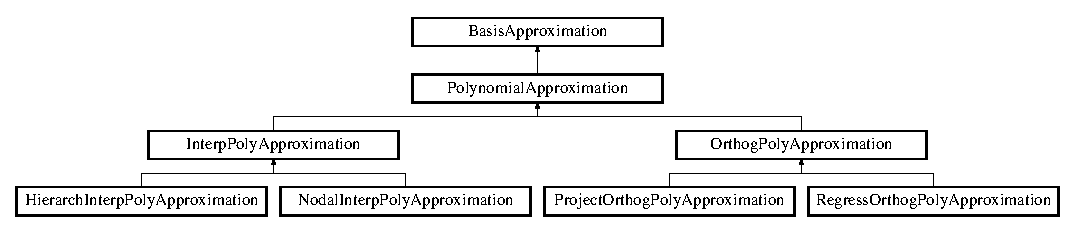
\includegraphics[height=2.666667cm]{classPecos_1_1BasisApproximation}
\end{center}
\end{figure}
\subsection*{Public Member Functions}
\begin{DoxyCompactItemize}
\item 
\hyperlink{classPecos_1_1BasisApproximation_a0f079f90460b078cfd553c20f2c33642}{Basis\+Approximation} ()
\begin{DoxyCompactList}\small\item\em default constructor \end{DoxyCompactList}\item 
\hyperlink{classPecos_1_1BasisApproximation_acc50081d826259352411322c65e1c2f2}{Basis\+Approximation} (const \hyperlink{classPecos_1_1SharedBasisApproxData}{Shared\+Basis\+Approx\+Data} \&shared\+\_\+data)
\begin{DoxyCompactList}\small\item\em standard constructor for envelope \end{DoxyCompactList}\item 
\hyperlink{classPecos_1_1BasisApproximation_afe92f553e027ee28cbb82dfb03ae5406}{Basis\+Approximation} (const \hyperlink{classPecos_1_1BasisApproximation}{Basis\+Approximation} \&basis\+\_\+approx)
\begin{DoxyCompactList}\small\item\em copy constructor \end{DoxyCompactList}\item 
virtual \hyperlink{classPecos_1_1BasisApproximation_ab820bed8a6adfca8d7888b6e17320c5e}{$\sim$\+Basis\+Approximation} ()
\begin{DoxyCompactList}\small\item\em destructor \end{DoxyCompactList}\item 
\hyperlink{classPecos_1_1BasisApproximation}{Basis\+Approximation} \hyperlink{classPecos_1_1BasisApproximation_a9f1c4e77a7c75f4004fa2e9af780a20e}{operator=} (const \hyperlink{classPecos_1_1BasisApproximation}{Basis\+Approximation} \&basis\+\_\+approx)
\begin{DoxyCompactList}\small\item\em assignment operator \end{DoxyCompactList}\item 
virtual Real \hyperlink{classPecos_1_1BasisApproximation_a7bc9dcdf32fc46f97e286268c1ac51b0}{value} (const Real\+Vector \&x)\label{classPecos_1_1BasisApproximation_a7bc9dcdf32fc46f97e286268c1ac51b0}

\begin{DoxyCompactList}\small\item\em retrieve the approximate function value for a given parameter vector \end{DoxyCompactList}\item 
virtual const Real\+Vector \& \hyperlink{classPecos_1_1BasisApproximation_a42bf374bf23c32c941ee2acae5ad56a4}{gradient} (const Real\+Vector \&x)\label{classPecos_1_1BasisApproximation_a42bf374bf23c32c941ee2acae5ad56a4}

\begin{DoxyCompactList}\small\item\em retrieve the approximate function gradient for a given parameter vector \end{DoxyCompactList}\item 
virtual const Real\+Sym\+Matrix \& \hyperlink{classPecos_1_1BasisApproximation_ad0b8d39aa7ec7b96b8753ac84e806d42}{hessian} (const Real\+Vector \&x)\label{classPecos_1_1BasisApproximation_ad0b8d39aa7ec7b96b8753ac84e806d42}

\begin{DoxyCompactList}\small\item\em retrieve the approximate function Hessian for a given parameter vector \end{DoxyCompactList}\item 
virtual void \hyperlink{classPecos_1_1BasisApproximation_aa1896011336650ae7b14965aebd72e1e}{surrogate\+\_\+data} (const Surrogate\+Data \&data)\label{classPecos_1_1BasisApproximation_aa1896011336650ae7b14965aebd72e1e}

\begin{DoxyCompactList}\small\item\em set \hyperlink{classPecos_1_1PolynomialApproximation_adea5235bed42287989f0bf6821f9bcf0}{Polynomial\+Approximation\+::orig\+Surr\+Data} \end{DoxyCompactList}\item 
virtual const Surrogate\+Data \& \hyperlink{classPecos_1_1BasisApproximation_a8b84d7f8e6de5203f20a47fa66b38ed3}{surrogate\+\_\+data} () const \label{classPecos_1_1BasisApproximation_a8b84d7f8e6de5203f20a47fa66b38ed3}

\begin{DoxyCompactList}\small\item\em get \hyperlink{classPecos_1_1PolynomialApproximation_a8e8d62a29dcb5dd55fd03bef1a2b3ea6}{Polynomial\+Approximation\+::surr\+Data} (const) \end{DoxyCompactList}\item 
virtual Surrogate\+Data \& \hyperlink{classPecos_1_1BasisApproximation_a0acf94a33f9a66b6823627d75ce566d4}{surrogate\+\_\+data} ()\label{classPecos_1_1BasisApproximation_a0acf94a33f9a66b6823627d75ce566d4}

\begin{DoxyCompactList}\small\item\em get \hyperlink{classPecos_1_1PolynomialApproximation_a8e8d62a29dcb5dd55fd03bef1a2b3ea6}{Polynomial\+Approximation\+::surr\+Data} (non-\/const) \end{DoxyCompactList}\item 
virtual int \hyperlink{classPecos_1_1BasisApproximation_ac789358ee49633613d6c97593be06f9d}{min\+\_\+coefficients} () const \label{classPecos_1_1BasisApproximation_ac789358ee49633613d6c97593be06f9d}

\begin{DoxyCompactList}\small\item\em return the minimum number of samples (unknowns) required to build the derived class approximation type in num\+Vars dimensions \end{DoxyCompactList}\item 
virtual void \hyperlink{classPecos_1_1BasisApproximation_aef8f0c32bdeff7756a9c614607c03058}{compute\+\_\+coefficients} (size\+\_\+t index=\+\_\+\+N\+P\+OS)\label{classPecos_1_1BasisApproximation_aef8f0c32bdeff7756a9c614607c03058}

\begin{DoxyCompactList}\small\item\em calculate the approximation coefficients using a set of surrogate data \end{DoxyCompactList}\item 
virtual void \hyperlink{classPecos_1_1BasisApproximation_a8ba12605934048176c1d1c5722465523}{increment\+\_\+coefficients} (size\+\_\+t index=\+\_\+\+N\+P\+OS)\label{classPecos_1_1BasisApproximation_a8ba12605934048176c1d1c5722465523}

\begin{DoxyCompactList}\small\item\em recalculate approximation coefficients following a surrogate data update \end{DoxyCompactList}\item 
virtual void \hyperlink{classPecos_1_1BasisApproximation_a662fd880fee0ed53f1e3383c41d6b792}{decrement\+\_\+coefficients} (bool save\+\_\+data)\label{classPecos_1_1BasisApproximation_a662fd880fee0ed53f1e3383c41d6b792}

\begin{DoxyCompactList}\small\item\em restore the approximation coefficients to the state preceding the last increment \end{DoxyCompactList}\item 
virtual void \hyperlink{classPecos_1_1BasisApproximation_a150c32326f6c12d2303806005715706e}{push\+\_\+coefficients} ()\label{classPecos_1_1BasisApproximation_a150c32326f6c12d2303806005715706e}

\begin{DoxyCompactList}\small\item\em restore the approximation coefficients to a previously incremented state as identified by the current data increment \end{DoxyCompactList}\item 
virtual void \hyperlink{classPecos_1_1BasisApproximation_a742e0217d6f681e08f401409771f4f4a}{finalize\+\_\+coefficients} ()\label{classPecos_1_1BasisApproximation_a742e0217d6f681e08f401409771f4f4a}

\begin{DoxyCompactList}\small\item\em finalize the coefficients by applying all previously evaluated increments \end{DoxyCompactList}\item 
virtual void \hyperlink{classPecos_1_1BasisApproximation_abc17a7104c33d8146f4a0ee7b6c6f37a}{store\+\_\+coefficients} (size\+\_\+t index=\+\_\+\+N\+P\+OS)\label{classPecos_1_1BasisApproximation_abc17a7104c33d8146f4a0ee7b6c6f37a}

\begin{DoxyCompactList}\small\item\em store the current coefficients for later combination \end{DoxyCompactList}\item 
virtual void \hyperlink{classPecos_1_1BasisApproximation_ad05b093ee96314c9e05bad8e06c2dae7}{restore\+\_\+coefficients} (size\+\_\+t index=\+\_\+\+N\+P\+OS)\label{classPecos_1_1BasisApproximation_ad05b093ee96314c9e05bad8e06c2dae7}

\begin{DoxyCompactList}\small\item\em restore a previously stored coefficient state \end{DoxyCompactList}\item 
virtual void \hyperlink{classPecos_1_1BasisApproximation_af5c6af74d2c8c5575fefb46ce55af90d}{swap\+\_\+coefficients} (size\+\_\+t index)\label{classPecos_1_1BasisApproximation_af5c6af74d2c8c5575fefb46ce55af90d}

\begin{DoxyCompactList}\small\item\em swap the current coefficients with a previously stored set \end{DoxyCompactList}\item 
virtual void \hyperlink{classPecos_1_1BasisApproximation_a63d12cc6021fda4896b8738d72dfcc86}{remove\+\_\+stored\+\_\+coefficients} (size\+\_\+t index=\+\_\+\+N\+P\+OS)\label{classPecos_1_1BasisApproximation_a63d12cc6021fda4896b8738d72dfcc86}

\begin{DoxyCompactList}\small\item\em remove a redundant stored entry prior to combine\+\_\+coefficients (default is pop\+\_\+back) \end{DoxyCompactList}\item 
virtual void \hyperlink{classPecos_1_1BasisApproximation_ae4337960917eda26a5672e5c6afbb62a}{clear\+\_\+stored} ()\label{classPecos_1_1BasisApproximation_ae4337960917eda26a5672e5c6afbb62a}

\begin{DoxyCompactList}\small\item\em clear stored approximation data \end{DoxyCompactList}\item 
virtual void \hyperlink{classPecos_1_1BasisApproximation_a7c794213befc83c9f90137f22e4cd39d}{combine\+\_\+coefficients} (size\+\_\+t swap\+\_\+index)\label{classPecos_1_1BasisApproximation_a7c794213befc83c9f90137f22e4cd39d}

\begin{DoxyCompactList}\small\item\em combine the current coefficients with a previously stored set \end{DoxyCompactList}\item 
virtual void \hyperlink{classPecos_1_1BasisApproximation_a4beb4a3300443171ac2233e87c970e39}{print\+\_\+coefficients} (std\+::ostream \&s, bool normalized)\label{classPecos_1_1BasisApproximation_a4beb4a3300443171ac2233e87c970e39}

\begin{DoxyCompactList}\small\item\em print the coefficient array computed in \hyperlink{classPecos_1_1BasisApproximation_aef8f0c32bdeff7756a9c614607c03058}{compute\+\_\+coefficients()} \end{DoxyCompactList}\item 
virtual Real\+Vector \hyperlink{classPecos_1_1BasisApproximation_ac64f16ff9fbfb80c4bafa969b4a92e1d}{approximation\+\_\+coefficients} (bool normalized) const \label{classPecos_1_1BasisApproximation_ac64f16ff9fbfb80c4bafa969b4a92e1d}

\begin{DoxyCompactList}\small\item\em return the coefficient array computed by \hyperlink{classPecos_1_1BasisApproximation_aef8f0c32bdeff7756a9c614607c03058}{compute\+\_\+coefficients()} \end{DoxyCompactList}\item 
virtual void \hyperlink{classPecos_1_1BasisApproximation_a2e7b82322962df3fd036b9e0783d8fc9}{approximation\+\_\+coefficients} (const Real\+Vector \&approx\+\_\+coeffs, bool normalized)\label{classPecos_1_1BasisApproximation_a2e7b82322962df3fd036b9e0783d8fc9}

\begin{DoxyCompactList}\small\item\em set the coefficient array from external sources, rather than computing with \hyperlink{classPecos_1_1BasisApproximation_aef8f0c32bdeff7756a9c614607c03058}{compute\+\_\+coefficients()} \end{DoxyCompactList}\item 
virtual void \hyperlink{classPecos_1_1BasisApproximation_a36020c0cf988e1af9f0e154af745f995}{coefficient\+\_\+labels} (std\+::vector$<$ std\+::string $>$ \&coeff\+\_\+labels) const \label{classPecos_1_1BasisApproximation_a36020c0cf988e1af9f0e154af745f995}

\begin{DoxyCompactList}\small\item\em retrieve a vector of coefficient label strings, one per expansion term \end{DoxyCompactList}\item 
void \hyperlink{classPecos_1_1BasisApproximation_a410dc797e6d458e8dde15e90802a6409}{assign\+\_\+rep} (\hyperlink{classPecos_1_1BasisApproximation}{Basis\+Approximation} $\ast$\hyperlink{classPecos_1_1BasisApproximation_a33f0a9133acdb15491e3288d92516d3a}{approx\+\_\+rep}, bool ref\+\_\+count\+\_\+incr)\label{classPecos_1_1BasisApproximation_a410dc797e6d458e8dde15e90802a6409}

\begin{DoxyCompactList}\small\item\em assign letter or replace existing letter with a new one \end{DoxyCompactList}\item 
\hyperlink{classPecos_1_1BasisApproximation}{Basis\+Approximation} $\ast$ \hyperlink{classPecos_1_1BasisApproximation_a33f0a9133acdb15491e3288d92516d3a}{approx\+\_\+rep} () const \label{classPecos_1_1BasisApproximation_a33f0a9133acdb15491e3288d92516d3a}

\begin{DoxyCompactList}\small\item\em returns approx\+Rep for access to derived class member functions that are not mapped to the top Approximation level \end{DoxyCompactList}\end{DoxyCompactItemize}
\subsection*{Protected Member Functions}
\begin{DoxyCompactItemize}
\item 
\hyperlink{classPecos_1_1BasisApproximation_adbf42e184a4775a594252c18d6bd903a}{Basis\+Approximation} (\hyperlink{structPecos_1_1BaseConstructor}{Base\+Constructor}, const \hyperlink{classPecos_1_1SharedBasisApproxData}{Shared\+Basis\+Approx\+Data} \&shared\+\_\+data)
\begin{DoxyCompactList}\small\item\em constructor initializes the base class part of letter classes (\hyperlink{structPecos_1_1BaseConstructor}{Base\+Constructor} overloading avoids infinite recursion in the derived class constructors -\/ Coplien, p. 139) \end{DoxyCompactList}\end{DoxyCompactItemize}
\subsection*{Protected Attributes}
\begin{DoxyCompactItemize}
\item 
\hyperlink{classPecos_1_1SharedBasisApproxData}{Shared\+Basis\+Approx\+Data} $\ast$ \hyperlink{classPecos_1_1BasisApproximation_a7ebf937967244f0702ead351cdcbe84d}{shared\+Data\+Rep}\label{classPecos_1_1BasisApproximation_a7ebf937967244f0702ead351cdcbe84d}

\begin{DoxyCompactList}\small\item\em contains the approximation data that is shared among the response set \end{DoxyCompactList}\end{DoxyCompactItemize}
\subsection*{Private Member Functions}
\begin{DoxyCompactItemize}
\item 
\hyperlink{classPecos_1_1BasisApproximation}{Basis\+Approximation} $\ast$ \hyperlink{classPecos_1_1BasisApproximation_a56018d7925e2d0d6a277bfd41c849820}{get\+\_\+basis\+\_\+approx} (const \hyperlink{classPecos_1_1SharedBasisApproxData}{Shared\+Basis\+Approx\+Data} \&shared\+\_\+data)
\begin{DoxyCompactList}\small\item\em Used only by the standard envelope constructor to initialize basis\+Approx\+Rep to the appropriate derived type. \end{DoxyCompactList}\end{DoxyCompactItemize}
\subsection*{Private Attributes}
\begin{DoxyCompactItemize}
\item 
\hyperlink{classPecos_1_1BasisApproximation}{Basis\+Approximation} $\ast$ \hyperlink{classPecos_1_1BasisApproximation_a4695a61501a689729db49ff5c498980a}{basis\+Approx\+Rep}\label{classPecos_1_1BasisApproximation_a4695a61501a689729db49ff5c498980a}

\begin{DoxyCompactList}\small\item\em pointer to the letter (initialized only for the envelope) \end{DoxyCompactList}\item 
int \hyperlink{classPecos_1_1BasisApproximation_afff0b6144883d3ca09a8d0d3f4776b0f}{reference\+Count}\label{classPecos_1_1BasisApproximation_afff0b6144883d3ca09a8d0d3f4776b0f}

\begin{DoxyCompactList}\small\item\em number of objects sharing basis\+Approx\+Rep \end{DoxyCompactList}\end{DoxyCompactItemize}


\subsection{Detailed Description}
Base class for multivariate basis approximations used for projection of random variables through time or space. 

The base class for basis approximations defined from Fourier functions, eigenfunctions, or polynomial functions. 

\subsection{Constructor \& Destructor Documentation}
\index{Pecos\+::\+Basis\+Approximation@{Pecos\+::\+Basis\+Approximation}!Basis\+Approximation@{Basis\+Approximation}}
\index{Basis\+Approximation@{Basis\+Approximation}!Pecos\+::\+Basis\+Approximation@{Pecos\+::\+Basis\+Approximation}}
\subsubsection[{\texorpdfstring{Basis\+Approximation()}{BasisApproximation()}}]{\setlength{\rightskip}{0pt plus 5cm}{\bf Basis\+Approximation} (
\begin{DoxyParamCaption}
{}
\end{DoxyParamCaption}
)}\label{classPecos_1_1BasisApproximation_a0f079f90460b078cfd553c20f2c33642}


default constructor 

The default constructor\+: basis\+Approx\+Rep is N\+U\+LL in this case. This makes it necessary to check for N\+U\+LL in the copy constructor, assignment operator, and destructor. \index{Pecos\+::\+Basis\+Approximation@{Pecos\+::\+Basis\+Approximation}!Basis\+Approximation@{Basis\+Approximation}}
\index{Basis\+Approximation@{Basis\+Approximation}!Pecos\+::\+Basis\+Approximation@{Pecos\+::\+Basis\+Approximation}}
\subsubsection[{\texorpdfstring{Basis\+Approximation(const Shared\+Basis\+Approx\+Data \&shared\+\_\+data)}{BasisApproximation(const SharedBasisApproxData &shared_data)}}]{\setlength{\rightskip}{0pt plus 5cm}{\bf Basis\+Approximation} (
\begin{DoxyParamCaption}
\item[{const {\bf Shared\+Basis\+Approx\+Data} \&}]{shared\+\_\+data}
\end{DoxyParamCaption}
)}\label{classPecos_1_1BasisApproximation_acc50081d826259352411322c65e1c2f2}


standard constructor for envelope 

Envelope constructor only needs to extract enough data to properly execute get\+\_\+basis\+\_\+approx, since Basis\+Approximation(\+Base\+Constructor) builds the actual base class data for the derived basis functions. 

References Basis\+Approximation\+::basis\+Approx\+Rep, and Basis\+Approximation\+::get\+\_\+basis\+\_\+approx().

\index{Pecos\+::\+Basis\+Approximation@{Pecos\+::\+Basis\+Approximation}!Basis\+Approximation@{Basis\+Approximation}}
\index{Basis\+Approximation@{Basis\+Approximation}!Pecos\+::\+Basis\+Approximation@{Pecos\+::\+Basis\+Approximation}}
\subsubsection[{\texorpdfstring{Basis\+Approximation(const Basis\+Approximation \&basis\+\_\+approx)}{BasisApproximation(const BasisApproximation &basis_approx)}}]{\setlength{\rightskip}{0pt plus 5cm}{\bf Basis\+Approximation} (
\begin{DoxyParamCaption}
\item[{const {\bf Basis\+Approximation} \&}]{basis\+\_\+approx}
\end{DoxyParamCaption}
)}\label{classPecos_1_1BasisApproximation_afe92f553e027ee28cbb82dfb03ae5406}


copy constructor 

Copy constructor manages sharing of basis\+Approx\+Rep and incrementing of reference\+Count. 

References Basis\+Approximation\+::basis\+Approx\+Rep, Basis\+Approximation\+::operator=(), and Basis\+Approximation\+::reference\+Count.

\index{Pecos\+::\+Basis\+Approximation@{Pecos\+::\+Basis\+Approximation}!````~Basis\+Approximation@{$\sim$\+Basis\+Approximation}}
\index{````~Basis\+Approximation@{$\sim$\+Basis\+Approximation}!Pecos\+::\+Basis\+Approximation@{Pecos\+::\+Basis\+Approximation}}
\subsubsection[{\texorpdfstring{$\sim$\+Basis\+Approximation()}{~BasisApproximation()}}]{\setlength{\rightskip}{0pt plus 5cm}$\sim${\bf Basis\+Approximation} (
\begin{DoxyParamCaption}
{}
\end{DoxyParamCaption}
)\hspace{0.3cm}{\ttfamily [virtual]}}\label{classPecos_1_1BasisApproximation_ab820bed8a6adfca8d7888b6e17320c5e}


destructor 

Destructor decrements reference\+Count and only deletes basis\+Approx\+Rep when reference\+Count reaches zero. 

References Basis\+Approximation\+::assign\+\_\+rep(), Basis\+Approximation\+::basis\+Approx\+Rep, and Basis\+Approximation\+::reference\+Count.

\index{Pecos\+::\+Basis\+Approximation@{Pecos\+::\+Basis\+Approximation}!Basis\+Approximation@{Basis\+Approximation}}
\index{Basis\+Approximation@{Basis\+Approximation}!Pecos\+::\+Basis\+Approximation@{Pecos\+::\+Basis\+Approximation}}
\subsubsection[{\texorpdfstring{Basis\+Approximation(\+Base\+Constructor, const Shared\+Basis\+Approx\+Data \&shared\+\_\+data)}{BasisApproximation(BaseConstructor, const SharedBasisApproxData &shared_data)}}]{\setlength{\rightskip}{0pt plus 5cm}{\bf Basis\+Approximation} (
\begin{DoxyParamCaption}
\item[{{\bf Base\+Constructor}}]{, }
\item[{const {\bf Shared\+Basis\+Approx\+Data} \&}]{shared\+\_\+data}
\end{DoxyParamCaption}
)\hspace{0.3cm}{\ttfamily [protected]}}\label{classPecos_1_1BasisApproximation_adbf42e184a4775a594252c18d6bd903a}


constructor initializes the base class part of letter classes (\hyperlink{structPecos_1_1BaseConstructor}{Base\+Constructor} overloading avoids infinite recursion in the derived class constructors -\/ Coplien, p. 139) 

This constructor is the one which must build the base class data for all derived classes. \hyperlink{classPecos_1_1BasisApproximation_a56018d7925e2d0d6a277bfd41c849820}{get\+\_\+basis\+\_\+approx()} instantiates a derived class letter and the derived constructor selects this base class constructor in its initialization list (to avoid recursion in the base class constructor calling \hyperlink{classPecos_1_1BasisApproximation_a56018d7925e2d0d6a277bfd41c849820}{get\+\_\+basis\+\_\+approx()} again). Since the letter IS the representation, its rep pointer is set to N\+U\+LL (an uninitialized pointer causes problems in $\sim$\+Basis\+Approximation). 

\subsection{Member Function Documentation}
\index{Pecos\+::\+Basis\+Approximation@{Pecos\+::\+Basis\+Approximation}!operator=@{operator=}}
\index{operator=@{operator=}!Pecos\+::\+Basis\+Approximation@{Pecos\+::\+Basis\+Approximation}}
\subsubsection[{\texorpdfstring{operator=(const Basis\+Approximation \&basis\+\_\+approx)}{operator=(const BasisApproximation &basis_approx)}}]{\setlength{\rightskip}{0pt plus 5cm}{\bf Basis\+Approximation} operator= (
\begin{DoxyParamCaption}
\item[{const {\bf Basis\+Approximation} \&}]{basis\+\_\+approx}
\end{DoxyParamCaption}
)}\label{classPecos_1_1BasisApproximation_a9f1c4e77a7c75f4004fa2e9af780a20e}


assignment operator 

Assignment operator decrements reference\+Count for old basis\+Approx\+Rep, assigns new basis\+Approx\+Rep, and increments reference\+Count for new basis\+Approx\+Rep. 

References Basis\+Approximation\+::basis\+Approx\+Rep, and Basis\+Approximation\+::reference\+Count.



Referenced by Basis\+Approximation\+::\+Basis\+Approximation().

\index{Pecos\+::\+Basis\+Approximation@{Pecos\+::\+Basis\+Approximation}!get\+\_\+basis\+\_\+approx@{get\+\_\+basis\+\_\+approx}}
\index{get\+\_\+basis\+\_\+approx@{get\+\_\+basis\+\_\+approx}!Pecos\+::\+Basis\+Approximation@{Pecos\+::\+Basis\+Approximation}}
\subsubsection[{\texorpdfstring{get\+\_\+basis\+\_\+approx(const Shared\+Basis\+Approx\+Data \&shared\+\_\+data)}{get_basis_approx(const SharedBasisApproxData &shared_data)}}]{\setlength{\rightskip}{0pt plus 5cm}{\bf Basis\+Approximation} $\ast$ get\+\_\+basis\+\_\+approx (
\begin{DoxyParamCaption}
\item[{const {\bf Shared\+Basis\+Approx\+Data} \&}]{shared\+\_\+data}
\end{DoxyParamCaption}
)\hspace{0.3cm}{\ttfamily [private]}}\label{classPecos_1_1BasisApproximation_a56018d7925e2d0d6a277bfd41c849820}


Used only by the standard envelope constructor to initialize basis\+Approx\+Rep to the appropriate derived type. 

Used only by the envelope constructor to initialize basis\+Approx\+Rep to the appropriate derived type. 

References Shared\+Basis\+Approx\+Data\+::basis\+Type, and Shared\+Basis\+Approx\+Data\+::data\+\_\+rep().



Referenced by Basis\+Approximation\+::\+Basis\+Approximation().



The documentation for this class was generated from the following files\+:\begin{DoxyCompactItemize}
\item 
Basis\+Approximation.\+hpp\item 
Basis\+Approximation.\+cpp\end{DoxyCompactItemize}

\section{Basis\+Config\+Options Class Reference}
\label{classPecos_1_1BasisConfigOptions}\index{Basis\+Config\+Options@{Basis\+Config\+Options}}


Container class for various basis configuration options.  


\subsection*{Public Member Functions}
\begin{DoxyCompactItemize}
\item 
\hyperlink{classPecos_1_1BasisConfigOptions_aab01805a888bbe54c41551f605b1b1fb}{Basis\+Config\+Options} ()\label{classPecos_1_1BasisConfigOptions_aab01805a888bbe54c41551f605b1b1fb}

\begin{DoxyCompactList}\small\item\em default constructor \end{DoxyCompactList}\item 
\hyperlink{classPecos_1_1BasisConfigOptions_a85bcdd68242189b0a986362296b8e3a9}{Basis\+Config\+Options} (bool nested\+\_\+rules, bool piecewise\+\_\+basis, bool equidistant\+\_\+rules, bool use\+\_\+derivs)\label{classPecos_1_1BasisConfigOptions_a85bcdd68242189b0a986362296b8e3a9}

\begin{DoxyCompactList}\small\item\em constructor \end{DoxyCompactList}\item 
\hyperlink{classPecos_1_1BasisConfigOptions_a92287b6200f91c9dacce4a3d1e3e9f98}{Basis\+Config\+Options} (const \hyperlink{classPecos_1_1BasisConfigOptions}{Basis\+Config\+Options} \&bc\+\_\+options)\label{classPecos_1_1BasisConfigOptions_a92287b6200f91c9dacce4a3d1e3e9f98}

\begin{DoxyCompactList}\small\item\em copy constructor \end{DoxyCompactList}\item 
\hyperlink{classPecos_1_1BasisConfigOptions_af794c3cf22cc067a10b5bc65ce1838cd}{$\sim$\+Basis\+Config\+Options} ()\label{classPecos_1_1BasisConfigOptions_af794c3cf22cc067a10b5bc65ce1838cd}

\begin{DoxyCompactList}\small\item\em destructor \end{DoxyCompactList}\end{DoxyCompactItemize}
\subsection*{Public Attributes}
\begin{DoxyCompactItemize}
\item 
bool \hyperlink{classPecos_1_1BasisConfigOptions_ae97d2f89ff8fe545aa9023279f71b5bc}{piecewise\+Basis}\label{classPecos_1_1BasisConfigOptions_ae97d2f89ff8fe545aa9023279f71b5bc}

\begin{DoxyCompactList}\small\item\em flag for use of piecewise basis polynomials \end{DoxyCompactList}\item 
bool \hyperlink{classPecos_1_1BasisConfigOptions_ad53c6bc00e92ff0e10ba3fd896c18a7d}{use\+Derivs}\label{classPecos_1_1BasisConfigOptions_ad53c6bc00e92ff0e10ba3fd896c18a7d}

\begin{DoxyCompactList}\small\item\em flag for utilizing derivatives during formation/calculation of expansions \end{DoxyCompactList}\item 
bool \hyperlink{classPecos_1_1BasisConfigOptions_aa53ad54ea1b8928e1a26ccd8505f59e9}{nested\+Rules}\label{classPecos_1_1BasisConfigOptions_aa53ad54ea1b8928e1a26ccd8505f59e9}

\begin{DoxyCompactList}\small\item\em flag for use of nested integration rules \end{DoxyCompactList}\item 
bool \hyperlink{classPecos_1_1BasisConfigOptions_ac594a3bb11101a1b117c756d84ebc14c}{equidistant\+Rules}\label{classPecos_1_1BasisConfigOptions_ac594a3bb11101a1b117c756d84ebc14c}

\begin{DoxyCompactList}\small\item\em flag for use of equidistant points for forming piecewise basis polynomials \end{DoxyCompactList}\item 
bool \hyperlink{classPecos_1_1BasisConfigOptions_abddb0ec628dbc665eb4b951b4cc473cc}{gauss\+Rule\+Override}\label{classPecos_1_1BasisConfigOptions_abddb0ec628dbc665eb4b951b4cc473cc}

\begin{DoxyCompactList}\small\item\em override interpolation rules to employ Gaussian quadrature \end{DoxyCompactList}\item 
bool \hyperlink{classPecos_1_1BasisConfigOptions_a534fdd21a453439193e1f1d6a372df46}{open\+Rule\+Override}\label{classPecos_1_1BasisConfigOptions_a534fdd21a453439193e1f1d6a372df46}

\begin{DoxyCompactList}\small\item\em override interpolation rules to employ open rules (e.\+g., Fejer2) \end{DoxyCompactList}\end{DoxyCompactItemize}


\subsection{Detailed Description}
Container class for various basis configuration options. 

The \hyperlink{classPecos_1_1BasisConfigOptions}{Basis\+Config\+Options} class provides a simple container class for basis configuration options related to rule nesting, piecewise basis polynomials, and derivative enhancement. 

The documentation for this class was generated from the following file\+:\begin{DoxyCompactItemize}
\item 
Shared\+Poly\+Approx\+Data.\+hpp\end{DoxyCompactItemize}

\section{Basis\+Polynomial Class Reference}
\label{classPecos_1_1BasisPolynomial}\index{Basis\+Polynomial@{Basis\+Polynomial}}


Base class for the basis polynomial class hierarchy.  


Inheritance diagram for Basis\+Polynomial\+:\begin{figure}[H]
\begin{center}
\leavevmode
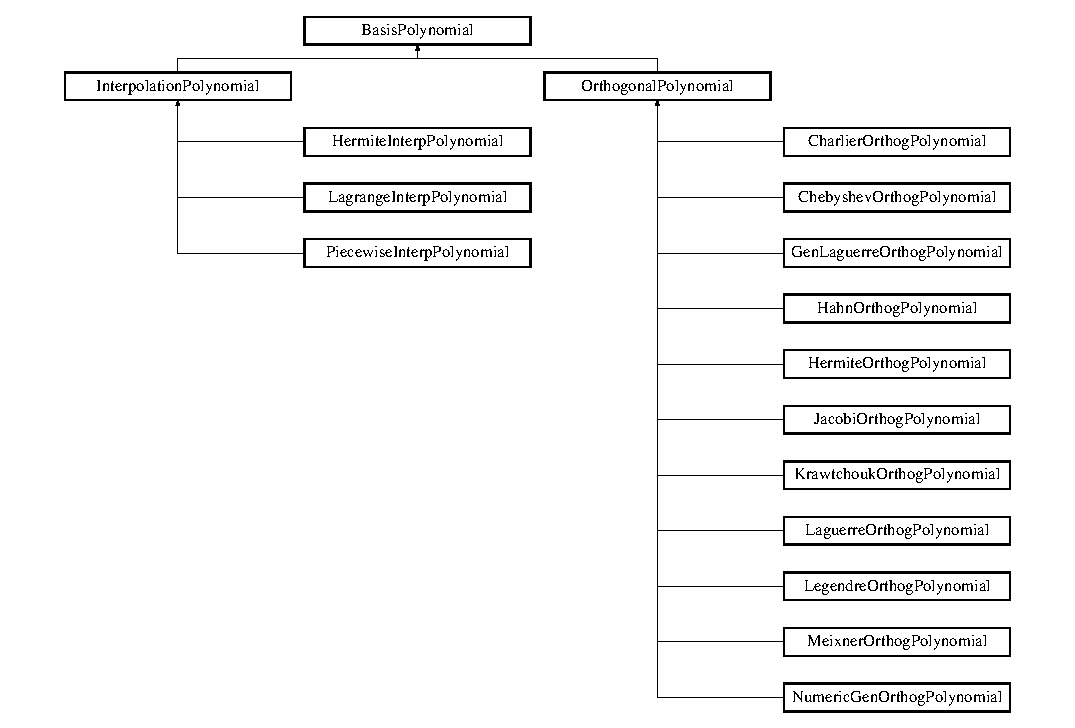
\includegraphics[height=9.333334cm]{classPecos_1_1BasisPolynomial}
\end{center}
\end{figure}
\subsection*{Public Member Functions}
\begin{DoxyCompactItemize}
\item 
\hyperlink{classPecos_1_1BasisPolynomial_a1e7f67828439e4044ba18c5b9ffe01c1}{Basis\+Polynomial} ()
\begin{DoxyCompactList}\small\item\em default constructor \end{DoxyCompactList}\item 
\hyperlink{classPecos_1_1BasisPolynomial_a321d05f6c985a7bb96bca1dc7e9460ce}{Basis\+Polynomial} (short poly\+\_\+type, short rule=0)
\begin{DoxyCompactList}\small\item\em alternate constructor \end{DoxyCompactList}\item 
\hyperlink{classPecos_1_1BasisPolynomial_a2c5e3388a9ea8cc44540efa900cc9069}{Basis\+Polynomial} (const \hyperlink{classPecos_1_1BasisPolynomial}{Basis\+Polynomial} \&polynomial)
\begin{DoxyCompactList}\small\item\em copy constructor \end{DoxyCompactList}\item 
virtual \hyperlink{classPecos_1_1BasisPolynomial_a9f799c229d1bdd891577e8840110aa0d}{$\sim$\+Basis\+Polynomial} ()
\begin{DoxyCompactList}\small\item\em destructor \end{DoxyCompactList}\item 
\hyperlink{classPecos_1_1BasisPolynomial}{Basis\+Polynomial} \hyperlink{classPecos_1_1BasisPolynomial_a662cf89a3c1958de60111435fd6c28d7}{operator=} (const \hyperlink{classPecos_1_1BasisPolynomial}{Basis\+Polynomial} \&polynomial)
\begin{DoxyCompactList}\small\item\em assignment operator \end{DoxyCompactList}\item 
virtual Real \hyperlink{classPecos_1_1BasisPolynomial_a5f87c364dcb43473f02b99b090d99cbb}{type1\+\_\+value} (unsigned short n)
\begin{DoxyCompactList}\small\item\em retrieve the value of the n\+\_\+th type 1 polynomial for a given parameter x using barycentric formulation \end{DoxyCompactList}\item 
virtual Real \hyperlink{classPecos_1_1BasisPolynomial_a1fab871e99cec3a1933a2b1e9ed8a625}{type1\+\_\+value} (Real x, unsigned short n)
\begin{DoxyCompactList}\small\item\em retrieve the value of the n\+\_\+th type 1 polynomial for a given parameter x using traditional characteristic polynomial formulation \end{DoxyCompactList}\item 
virtual Real \hyperlink{classPecos_1_1BasisPolynomial_aecd19f4bde44ba0cc371340405d81a18}{type2\+\_\+value} (Real x, unsigned short n)
\begin{DoxyCompactList}\small\item\em retrieve the value of the n\+\_\+th type 2 polynomial for a given parameter x \end{DoxyCompactList}\item 
virtual Real \hyperlink{classPecos_1_1BasisPolynomial_ac88b2920bdede895a618385160254741}{type1\+\_\+gradient} (unsigned short n)
\begin{DoxyCompactList}\small\item\em retrieve the gradient of the n\+\_\+th type 1 polynomial for a given parameter x using barycentric formulation \end{DoxyCompactList}\item 
virtual Real \hyperlink{classPecos_1_1BasisPolynomial_a6f69ec84983f551e7e0e4a18b78b4498}{type1\+\_\+gradient} (Real x, unsigned short n)
\begin{DoxyCompactList}\small\item\em retrieve the gradient of the n\+\_\+th type 1 polynomial for a given parameter x using traditional characteristic polynomial formulation \end{DoxyCompactList}\item 
virtual Real \hyperlink{classPecos_1_1BasisPolynomial_a3a6b82f9baaa857ff03ea5a63ff48cc8}{type2\+\_\+gradient} (Real x, unsigned short n)
\begin{DoxyCompactList}\small\item\em retrieve the gradient of the n\+\_\+th type 2 polynomial for a given parameter x \end{DoxyCompactList}\item 
virtual Real \hyperlink{classPecos_1_1BasisPolynomial_a07d617dad8572dd606371e6c89ab6c35}{type1\+\_\+hessian} (Real x, unsigned short n)
\begin{DoxyCompactList}\small\item\em retrieve the Hessian of the n\+\_\+th type 1 polynomial for a given parameter x using traditional characteristic polynomial formulation \end{DoxyCompactList}\item 
virtual Real \hyperlink{classPecos_1_1BasisPolynomial_ab74383be309d74823f2e5e85dad739b2}{norm\+\_\+squared} (unsigned short n)
\begin{DoxyCompactList}\small\item\em returns the norm-\/squared of the n\+\_\+th order polynomial defined by the inner product $<$Poly\+\_\+n, Poly\+\_\+n$>$ = $\vert$$\vert$\+Poly\+\_\+n$\vert$$\vert$$^\wedge$2 \end{DoxyCompactList}\item 
virtual const Real\+Array \& \hyperlink{classPecos_1_1BasisPolynomial_a0f96bd4e27ddc5c44117e7b68744b5a4}{collocation\+\_\+points} (unsigned short n)
\begin{DoxyCompactList}\small\item\em return collocation points corresponding to orthogonal polynomial order n \end{DoxyCompactList}\item 
virtual const Real\+Array \& \hyperlink{classPecos_1_1BasisPolynomial_aa010321cf47465dca5725fa15ba58bf6}{type1\+\_\+collocation\+\_\+weights} (unsigned short order)
\begin{DoxyCompactList}\small\item\em return the type 1 collocation weights corresponding to a point set of size order \end{DoxyCompactList}\item 
virtual const Real\+Array \& \hyperlink{classPecos_1_1BasisPolynomial_a8bc6cc516ab2bccbbdca6e904dc5a10f}{type2\+\_\+collocation\+\_\+weights} (unsigned short order)
\begin{DoxyCompactList}\small\item\em return the type 2 collocation weights corresponding to a point set of size order \end{DoxyCompactList}\item 
virtual void \hyperlink{classPecos_1_1BasisPolynomial_afdf46109d433281e37d3de26f4bd1b3d}{set\+\_\+new\+\_\+point} (Real x, short order)\label{classPecos_1_1BasisPolynomial_afdf46109d433281e37d3de26f4bd1b3d}

\begin{DoxyCompactList}\small\item\em for barycentric interpolation, set the point to be interpolated for purposes of precomputation of nodal value/gradient factors \end{DoxyCompactList}\item 
virtual void \hyperlink{classPecos_1_1BasisPolynomial_a01ad737aacfeb1918ffae9b52323336a}{set\+\_\+new\+\_\+point} (Real x, short order, const U\+Short\+Array \&delta\+\_\+key)\label{classPecos_1_1BasisPolynomial_a01ad737aacfeb1918ffae9b52323336a}

\begin{DoxyCompactList}\small\item\em for barycentric interpolation, set the point to be interpolated for purposes of precomputation of hierarchical value/gradient factors \end{DoxyCompactList}\item 
virtual size\+\_\+t \hyperlink{classPecos_1_1BasisPolynomial_aed1b9a98e9f80287b21581e7278aa253}{exact\+\_\+index} () const \label{classPecos_1_1BasisPolynomial_aed1b9a98e9f80287b21581e7278aa253}

\begin{DoxyCompactList}\small\item\em returns the index of a collocation point that is an exact match with the point to be interpolated (from \hyperlink{classPecos_1_1BasisPolynomial_afdf46109d433281e37d3de26f4bd1b3d}{set\+\_\+new\+\_\+point()}) if detected (\+\_\+\+N\+P\+OS if not) \end{DoxyCompactList}\item 
virtual size\+\_\+t \hyperlink{classPecos_1_1BasisPolynomial_a90937bbedd0d5c002f5015cf3847cbaf}{exact\+\_\+delta\+\_\+index} () const \label{classPecos_1_1BasisPolynomial_a90937bbedd0d5c002f5015cf3847cbaf}

\begin{DoxyCompactList}\small\item\em returns the index of a hierarchical increment to the interpolation points that is an exact match with the point to be interpolated (from \hyperlink{classPecos_1_1BasisPolynomial_afdf46109d433281e37d3de26f4bd1b3d}{set\+\_\+new\+\_\+point()}) if detected (\+\_\+\+N\+P\+OS if not) \end{DoxyCompactList}\item 
virtual const Real\+Vector \& \hyperlink{classPecos_1_1BasisPolynomial_ab95f72f936b15b2f4cecde96d34d798c}{barycentric\+\_\+value\+\_\+factors} () const \label{classPecos_1_1BasisPolynomial_ab95f72f936b15b2f4cecde96d34d798c}

\begin{DoxyCompactList}\small\item\em return the barycentric value factors \end{DoxyCompactList}\item 
virtual Real \hyperlink{classPecos_1_1BasisPolynomial_a72c4d54d2ef767ab8329f1fb67c7a3fe}{barycentric\+\_\+value\+\_\+factor} (unsigned short i) const \label{classPecos_1_1BasisPolynomial_a72c4d54d2ef767ab8329f1fb67c7a3fe}

\begin{DoxyCompactList}\small\item\em return a particular barycentric value factor \end{DoxyCompactList}\item 
virtual const Real\+Vector \& \hyperlink{classPecos_1_1BasisPolynomial_a1f77beaf45743dce80d8253b8f7a9394}{barycentric\+\_\+gradient\+\_\+factors} () const \label{classPecos_1_1BasisPolynomial_a1f77beaf45743dce80d8253b8f7a9394}

\begin{DoxyCompactList}\small\item\em return the barycentric gradient factors \end{DoxyCompactList}\item 
virtual Real \hyperlink{classPecos_1_1BasisPolynomial_a9cd03b3dfa402dcb120423d116e07d6b}{barycentric\+\_\+gradient\+\_\+factor} (unsigned short i) const \label{classPecos_1_1BasisPolynomial_a9cd03b3dfa402dcb120423d116e07d6b}

\begin{DoxyCompactList}\small\item\em return a particular barycentric gradient factor \end{DoxyCompactList}\item 
virtual Real \hyperlink{classPecos_1_1BasisPolynomial_ad36b23949c632dd0a6784f82f90050e4}{barycentric\+\_\+value\+\_\+factor\+\_\+sum} () const \label{classPecos_1_1BasisPolynomial_ad36b23949c632dd0a6784f82f90050e4}

\begin{DoxyCompactList}\small\item\em return the sum of all barycentric value factors for use in computing the barycentric interpolant denominator \end{DoxyCompactList}\item 
virtual Real \hyperlink{classPecos_1_1BasisPolynomial_ae0b1d51779230f3ce9fe3d7c4fc14198}{barycentric\+\_\+difference\+\_\+product} () const \label{classPecos_1_1BasisPolynomial_ae0b1d51779230f3ce9fe3d7c4fc14198}

\begin{DoxyCompactList}\small\item\em return the product of all differences between the interpolation points and a current point \end{DoxyCompactList}\item 
virtual void \hyperlink{classPecos_1_1BasisPolynomial_ad6115367af3811a5c75acbe340f04e58}{reset\+\_\+gauss} ()
\begin{DoxyCompactList}\small\item\em destroy history of Gauss pts/wts (due to distribution parameter changes) \end{DoxyCompactList}\item 
virtual Real \hyperlink{classPecos_1_1BasisPolynomial_ae2d76fe489a1633b6854399565692131}{point\+\_\+factor} ()\label{classPecos_1_1BasisPolynomial_ae2d76fe489a1633b6854399565692131}

\begin{DoxyCompactList}\small\item\em (calculate and) return pt\+Factor \end{DoxyCompactList}\item 
virtual Real \hyperlink{classPecos_1_1BasisPolynomial_acc5475d6b992e443e3cce753a48cfc32}{weight\+\_\+factor} ()\label{classPecos_1_1BasisPolynomial_acc5475d6b992e443e3cce753a48cfc32}

\begin{DoxyCompactList}\small\item\em (calculate and) return wt\+Factor \end{DoxyCompactList}\item 
virtual Real \hyperlink{classPecos_1_1BasisPolynomial_a997bdeddf670667c476513fcacc779ca}{alpha\+\_\+polynomial} () const 
\begin{DoxyCompactList}\small\item\em return \{Jacobi,Gen\+Laguerre\}Orthog\+Polynomial\+::alpha\+Poly \end{DoxyCompactList}\item 
virtual Real \hyperlink{classPecos_1_1BasisPolynomial_a22bfc4209dec76716ef51648e945469a}{beta\+\_\+polynomial} () const 
\begin{DoxyCompactList}\small\item\em return \hyperlink{classPecos_1_1JacobiOrthogPolynomial_a96c0b0201ca445f95be14ec035b595cb}{Jacobi\+Orthog\+Polynomial\+::beta\+Poly} \end{DoxyCompactList}\item 
virtual void \hyperlink{classPecos_1_1BasisPolynomial_aeeb4ce11a8d413209be1ec08eced8728}{alpha\+\_\+stat} (Real alpha)
\begin{DoxyCompactList}\small\item\em set \hyperlink{classPecos_1_1JacobiOrthogPolynomial_a96c0b0201ca445f95be14ec035b595cb}{Jacobi\+Orthog\+Polynomial\+::beta\+Poly} or \hyperlink{classPecos_1_1GenLaguerreOrthogPolynomial_a11666846719189915a02ac6f1f96e393}{Gen\+Laguerre\+Orthog\+Polynomial\+::alpha\+Poly} from statistical defn of alpha \end{DoxyCompactList}\item 
virtual void \hyperlink{classPecos_1_1BasisPolynomial_a7f9584e538ee1574bd4d8d1afb622ed6}{beta\+\_\+stat} (Real beta)
\begin{DoxyCompactList}\small\item\em set \hyperlink{classPecos_1_1JacobiOrthogPolynomial_a11666846719189915a02ac6f1f96e393}{Jacobi\+Orthog\+Polynomial\+::alpha\+Poly} from statistical defn of beta \end{DoxyCompactList}\item 
virtual void \hyperlink{classPecos_1_1BasisPolynomial_addd13d4093ce8cbf2d22c47a47aff610}{collocation\+\_\+rule} (short rule)\label{classPecos_1_1BasisPolynomial_addd13d4093ce8cbf2d22c47a47aff610}

\begin{DoxyCompactList}\small\item\em set \hyperlink{classPecos_1_1OrthogonalPolynomial_abcc1d84cc8e8c8b5a66f720067039f2e}{Orthogonal\+Polynomial\+::colloc\+Rule} \end{DoxyCompactList}\item 
virtual short \hyperlink{classPecos_1_1BasisPolynomial_a2e390f265fcc800348dc816d6cc37f86}{collocation\+\_\+rule} () const \label{classPecos_1_1BasisPolynomial_a2e390f265fcc800348dc816d6cc37f86}

\begin{DoxyCompactList}\small\item\em get \hyperlink{classPecos_1_1OrthogonalPolynomial_abcc1d84cc8e8c8b5a66f720067039f2e}{Orthogonal\+Polynomial\+::colloc\+Rule} \end{DoxyCompactList}\item 
virtual size\+\_\+t \hyperlink{classPecos_1_1BasisPolynomial_a3122d8fb10bc54de12fde87cffdf8fee}{interpolation\+\_\+size} () const 
\begin{DoxyCompactList}\small\item\em get size of \hyperlink{classPecos_1_1InterpolationPolynomial_ae944308ccb32a77df689397d462470b4}{Interpolation\+Polynomial\+::interp\+Pts} \end{DoxyCompactList}\item 
virtual void \hyperlink{classPecos_1_1BasisPolynomial_a7e9e8124500425e8435b9b0ffa0c2eb2}{interpolation\+\_\+points} (const Real\+Array \&interpolation\+\_\+pts)
\begin{DoxyCompactList}\small\item\em set \hyperlink{classPecos_1_1InterpolationPolynomial_ae944308ccb32a77df689397d462470b4}{Interpolation\+Polynomial\+::interp\+Pts} \end{DoxyCompactList}\item 
virtual const Real\+Array \& \hyperlink{classPecos_1_1BasisPolynomial_af8e63614c42281644c4c0e099fb3e1f8}{interpolation\+\_\+points} () const 
\begin{DoxyCompactList}\small\item\em get \hyperlink{classPecos_1_1InterpolationPolynomial_ae944308ccb32a77df689397d462470b4}{Interpolation\+Polynomial\+::interp\+Pts} \end{DoxyCompactList}\item 
virtual bool \hyperlink{classPecos_1_1BasisPolynomial_abc2afafc150f648667a41e0ce656b6da}{parameterized} () const \label{classPecos_1_1BasisPolynomial_abc2afafc150f648667a41e0ce656b6da}

\begin{DoxyCompactList}\small\item\em return whether a derived \hyperlink{classPecos_1_1BasisPolynomial}{Basis\+Polynomial} type supports parameterization \end{DoxyCompactList}\item 
virtual Real \hyperlink{classPecos_1_1BasisPolynomial_a8c1e8d014e82efc5a1c20f973b5bc715}{length\+\_\+scale} () const \label{classPecos_1_1BasisPolynomial_a8c1e8d014e82efc5a1c20f973b5bc715}

\begin{DoxyCompactList}\small\item\em return a characteristic length scale for the probability distribution associated with an orthogonal polynomial basis \end{DoxyCompactList}\item 
virtual void \hyperlink{classPecos_1_1BasisPolynomial_ad1f50a6d03d3b48687bf9c4ca889b389}{precompute\+\_\+rules} (unsigned short order)\label{classPecos_1_1BasisPolynomial_ad1f50a6d03d3b48687bf9c4ca889b389}

\begin{DoxyCompactList}\small\item\em precompute quadrature rules up to specified order \end{DoxyCompactList}\item 
short \hyperlink{classPecos_1_1BasisPolynomial_a5f8d739fc54e733bc9bfb7017234c82c}{basis\+\_\+type} () const \label{classPecos_1_1BasisPolynomial_a5f8d739fc54e733bc9bfb7017234c82c}

\begin{DoxyCompactList}\small\item\em return basis\+Poly\+Type \end{DoxyCompactList}\item 
bool \hyperlink{classPecos_1_1BasisPolynomial_a6e1b9ff4ca6f1269bb739b0de9e14dab}{parametric\+\_\+update} () const \label{classPecos_1_1BasisPolynomial_a6e1b9ff4ca6f1269bb739b0de9e14dab}

\begin{DoxyCompactList}\small\item\em return parametric\+Update \end{DoxyCompactList}\item 
\hyperlink{classPecos_1_1BasisPolynomial}{Basis\+Polynomial} $\ast$ \hyperlink{classPecos_1_1BasisPolynomial_ae1736d9eb56f44e3b85cc7c17a086de2}{polynomial\+\_\+rep} () const \label{classPecos_1_1BasisPolynomial_ae1736d9eb56f44e3b85cc7c17a086de2}

\begin{DoxyCompactList}\small\item\em returns poly\+Rep for access to derived class member functions that are not mapped to the top \hyperlink{classPecos_1_1BasisPolynomial}{Basis\+Polynomial} level \end{DoxyCompactList}\item 
bool \hyperlink{classPecos_1_1BasisPolynomial_a3c45461717ff230edd665ce24da988c5}{is\+\_\+null} () const \label{classPecos_1_1BasisPolynomial_a3c45461717ff230edd665ce24da988c5}

\begin{DoxyCompactList}\small\item\em function to check poly\+Rep (does this handle contain a body) \end{DoxyCompactList}\end{DoxyCompactItemize}
\subsection*{Static Public Member Functions}
\begin{DoxyCompactItemize}
\item 
static Real \hyperlink{classPecos_1_1BasisPolynomial_a7faa05dcc03d3434fab2f7c6daea214c}{factorial} (unsigned short n)
\begin{DoxyCompactList}\small\item\em compute n! \end{DoxyCompactList}\item 
static Real \hyperlink{classPecos_1_1BasisPolynomial_a664cfe6495b3288d61da655623e1bc1b}{factorial\+\_\+ratio} (unsigned short num, unsigned short den)
\begin{DoxyCompactList}\small\item\em compute num!/den! \end{DoxyCompactList}\item 
static Real \hyperlink{classPecos_1_1BasisPolynomial_a7dd442a31465f57d8d60a7d8dc581376}{n\+\_\+choose\+\_\+k} (unsigned short n, unsigned short k)
\begin{DoxyCompactList}\small\item\em compute n!/(k!(n-\/k)!) \end{DoxyCompactList}\item 
static Real \hyperlink{classPecos_1_1BasisPolynomial_ad881b3d21f02cbe840663f1d57f717d4}{pochhammer} (Real m, unsigned short n)
\begin{DoxyCompactList}\small\item\em compute the Pochhammer symbol (m)\+\_\+n = m$\ast$(m+1)...$\ast$(m+n-\/1) \end{DoxyCompactList}\end{DoxyCompactItemize}
\subsection*{Protected Member Functions}
\begin{DoxyCompactItemize}
\item 
\hyperlink{classPecos_1_1BasisPolynomial_a483dd35abaf764ce50b3c807390be280}{Basis\+Polynomial} (\hyperlink{structPecos_1_1BaseConstructor}{Base\+Constructor})
\begin{DoxyCompactList}\small\item\em constructor initializes the base class part of letter classes (\hyperlink{structPecos_1_1BaseConstructor}{Base\+Constructor} overloading avoids infinite recursion in the derived class constructors -\/ Coplien, p. 139) \end{DoxyCompactList}\end{DoxyCompactItemize}
\subsection*{Protected Attributes}
\begin{DoxyCompactItemize}
\item 
short \hyperlink{classPecos_1_1BasisPolynomial_a53acc6b4e7a4c8b16acc679e875bed35}{basis\+Poly\+Type}\label{classPecos_1_1BasisPolynomial_a53acc6b4e7a4c8b16acc679e875bed35}

\begin{DoxyCompactList}\small\item\em basis polynomial type\+: \{H\+E\+R\+M\+I\+TE,L\+E\+G\+E\+N\+D\+RE,L\+A\+G\+U\+E\+R\+RE,J\+A\+C\+O\+BI,G\+E\+N\+\_\+\+L\+A\+G\+U\+E\+R\+RE,N\+U\+M\+\_\+\+G\+EN\}\+\_\+\+O\+R\+T\+H\+OG, \{L\+A\+G\+R\+A\+N\+GE,H\+E\+R\+M\+I\+TE\}\+\_\+\+I\+N\+T\+E\+RP, or P\+I\+E\+C\+E\+W\+I\+S\+E\+\_\+\{L\+I\+N\+E\+AR,Q\+U\+A\+D\+R\+A\+T\+IC,C\+U\+B\+IC\}\+\_\+\+I\+N\+T\+E\+RP \end{DoxyCompactList}\item 
bool \hyperlink{classPecos_1_1BasisPolynomial_aa46c2df8f8cb2bdb4d2193fca54d19a5}{parametric\+Update}\label{classPecos_1_1BasisPolynomial_aa46c2df8f8cb2bdb4d2193fca54d19a5}

\begin{DoxyCompactList}\small\item\em flag indicating presence of a parametric update to the basis polynomial, such that previous points/weights may not be reused \end{DoxyCompactList}\item 
Real \hyperlink{classPecos_1_1BasisPolynomial_a51c13e36e22c4aa68e0c555eea44ed34}{wt\+Factor}\label{classPecos_1_1BasisPolynomial_a51c13e36e22c4aa68e0c555eea44ed34}

\begin{DoxyCompactList}\small\item\em weight discrepancy factor between Abramowitz-\/\+Stegun and P\+DF orthogonality \end{DoxyCompactList}\item 
Real \hyperlink{classPecos_1_1BasisPolynomial_a8ea6ec2f6b4e706218ad44e5914c8632}{pt\+Factor}\label{classPecos_1_1BasisPolynomial_a8ea6ec2f6b4e706218ad44e5914c8632}

\begin{DoxyCompactList}\small\item\em point discrepancy factor between Abramowitz-\/\+Stegun and P\+DF orthogonality \end{DoxyCompactList}\end{DoxyCompactItemize}
\subsection*{Private Member Functions}
\begin{DoxyCompactItemize}
\item 
\hyperlink{classPecos_1_1BasisPolynomial}{Basis\+Polynomial} $\ast$ \hyperlink{classPecos_1_1BasisPolynomial_a76cffba3f7273eb68941a640363a6209}{get\+\_\+polynomial} (short poly\+\_\+type, short rule)
\begin{DoxyCompactList}\small\item\em Used by the envelope constructor to initialize poly\+Rep to the appropriate derived type. \end{DoxyCompactList}\end{DoxyCompactItemize}
\subsection*{Private Attributes}
\begin{DoxyCompactItemize}
\item 
\hyperlink{classPecos_1_1BasisPolynomial}{Basis\+Polynomial} $\ast$ \hyperlink{classPecos_1_1BasisPolynomial_a48a3787994e61838201fcfc71e2f1a54}{poly\+Rep}\label{classPecos_1_1BasisPolynomial_a48a3787994e61838201fcfc71e2f1a54}

\begin{DoxyCompactList}\small\item\em pointer to the letter (initialized only for the envelope) \end{DoxyCompactList}\item 
int \hyperlink{classPecos_1_1BasisPolynomial_afff0b6144883d3ca09a8d0d3f4776b0f}{reference\+Count}\label{classPecos_1_1BasisPolynomial_afff0b6144883d3ca09a8d0d3f4776b0f}

\begin{DoxyCompactList}\small\item\em number of objects sharing poly\+Rep \end{DoxyCompactList}\end{DoxyCompactItemize}


\subsection{Detailed Description}
Base class for the basis polynomial class hierarchy. 

The \hyperlink{classPecos_1_1BasisPolynomial}{Basis\+Polynomial} class is the base class for the univariate basis polynomial class hierarchy in P\+E\+C\+OS. One instance of an \hyperlink{classPecos_1_1BasisPolynomial}{Basis\+Polynomial} is created for each variable within a multidimensional polynomial basis function (a vector of Basis\+Polynomials is contained in Basis\+Poly\+Approximation, which may be mixed and matched in, e.\+g., the Wiener-\/\+Askey scheme for polynomial chaos). For memory efficiency and enhanced polymorphism, the basis polynomial hierarchy employs the \char`\"{}letter/envelope idiom\char`\"{} (see Coplien \char`\"{}\+Advanced C++\char`\"{}, p. 133), for which the base class (\hyperlink{classPecos_1_1BasisPolynomial}{Basis\+Polynomial}) serves as the envelope and one of the derived classes (selected in \hyperlink{classPecos_1_1BasisPolynomial_a76cffba3f7273eb68941a640363a6209}{Basis\+Polynomial\+::get\+\_\+polynomial()}) serves as the letter. 

\subsection{Constructor \& Destructor Documentation}
\index{Pecos\+::\+Basis\+Polynomial@{Pecos\+::\+Basis\+Polynomial}!Basis\+Polynomial@{Basis\+Polynomial}}
\index{Basis\+Polynomial@{Basis\+Polynomial}!Pecos\+::\+Basis\+Polynomial@{Pecos\+::\+Basis\+Polynomial}}
\subsubsection[{\texorpdfstring{Basis\+Polynomial()}{BasisPolynomial()}}]{\setlength{\rightskip}{0pt plus 5cm}{\bf Basis\+Polynomial} (
\begin{DoxyParamCaption}
{}
\end{DoxyParamCaption}
)}\label{classPecos_1_1BasisPolynomial_a1e7f67828439e4044ba18c5b9ffe01c1}


default constructor 

The default constructor is used in Array$<$\+Basis\+Polynomial$>$ instantiations and by the alternate envelope constructor. poly\+Rep is N\+U\+LL in this case (problem\+\_\+db is needed to build a meaningful instance). This makes it necessary to check for N\+U\+LL in the copy constructor, assignment operator, and destructor. \index{Pecos\+::\+Basis\+Polynomial@{Pecos\+::\+Basis\+Polynomial}!Basis\+Polynomial@{Basis\+Polynomial}}
\index{Basis\+Polynomial@{Basis\+Polynomial}!Pecos\+::\+Basis\+Polynomial@{Pecos\+::\+Basis\+Polynomial}}
\subsubsection[{\texorpdfstring{Basis\+Polynomial(short poly\+\_\+type, short rule=0)}{BasisPolynomial(short poly_type, short rule=0)}}]{\setlength{\rightskip}{0pt plus 5cm}{\bf Basis\+Polynomial} (
\begin{DoxyParamCaption}
\item[{short}]{poly\+\_\+type, }
\item[{short}]{rule = {\ttfamily 0}}
\end{DoxyParamCaption}
)}\label{classPecos_1_1BasisPolynomial_a321d05f6c985a7bb96bca1dc7e9460ce}


alternate constructor 

Envelope constructor which does not require access to problem\+\_\+db. This constructor executes get\+\_\+polynomial(type), which invokes the default constructor of the derived letter class, which in turn invokes the \hyperlink{structPecos_1_1BaseConstructor}{Base\+Constructor} of the base class. 

References Basis\+Polynomial\+::get\+\_\+polynomial(), and Basis\+Polynomial\+::poly\+Rep.

\index{Pecos\+::\+Basis\+Polynomial@{Pecos\+::\+Basis\+Polynomial}!Basis\+Polynomial@{Basis\+Polynomial}}
\index{Basis\+Polynomial@{Basis\+Polynomial}!Pecos\+::\+Basis\+Polynomial@{Pecos\+::\+Basis\+Polynomial}}
\subsubsection[{\texorpdfstring{Basis\+Polynomial(const Basis\+Polynomial \&polynomial)}{BasisPolynomial(const BasisPolynomial &polynomial)}}]{\setlength{\rightskip}{0pt plus 5cm}{\bf Basis\+Polynomial} (
\begin{DoxyParamCaption}
\item[{const {\bf Basis\+Polynomial} \&}]{polynomial}
\end{DoxyParamCaption}
)}\label{classPecos_1_1BasisPolynomial_a2c5e3388a9ea8cc44540efa900cc9069}


copy constructor 

Copy constructor manages sharing of poly\+Rep and incrementing of reference\+Count. 

References Basis\+Polynomial\+::poly\+Rep, and Basis\+Polynomial\+::reference\+Count.

\index{Pecos\+::\+Basis\+Polynomial@{Pecos\+::\+Basis\+Polynomial}!````~Basis\+Polynomial@{$\sim$\+Basis\+Polynomial}}
\index{````~Basis\+Polynomial@{$\sim$\+Basis\+Polynomial}!Pecos\+::\+Basis\+Polynomial@{Pecos\+::\+Basis\+Polynomial}}
\subsubsection[{\texorpdfstring{$\sim$\+Basis\+Polynomial()}{~BasisPolynomial()}}]{\setlength{\rightskip}{0pt plus 5cm}$\sim${\bf Basis\+Polynomial} (
\begin{DoxyParamCaption}
{}
\end{DoxyParamCaption}
)\hspace{0.3cm}{\ttfamily [virtual]}}\label{classPecos_1_1BasisPolynomial_a9f799c229d1bdd891577e8840110aa0d}


destructor 

Destructor decrements reference\+Count and only deletes poly\+Rep when reference\+Count reaches zero. 

References Basis\+Polynomial\+::poly\+Rep, and Basis\+Polynomial\+::reference\+Count.

\index{Pecos\+::\+Basis\+Polynomial@{Pecos\+::\+Basis\+Polynomial}!Basis\+Polynomial@{Basis\+Polynomial}}
\index{Basis\+Polynomial@{Basis\+Polynomial}!Pecos\+::\+Basis\+Polynomial@{Pecos\+::\+Basis\+Polynomial}}
\subsubsection[{\texorpdfstring{Basis\+Polynomial(\+Base\+Constructor)}{BasisPolynomial(BaseConstructor)}}]{\setlength{\rightskip}{0pt plus 5cm}{\bf Basis\+Polynomial} (
\begin{DoxyParamCaption}
\item[{{\bf Base\+Constructor}}]{}
\end{DoxyParamCaption}
)\hspace{0.3cm}{\ttfamily [protected]}}\label{classPecos_1_1BasisPolynomial_a483dd35abaf764ce50b3c807390be280}


constructor initializes the base class part of letter classes (\hyperlink{structPecos_1_1BaseConstructor}{Base\+Constructor} overloading avoids infinite recursion in the derived class constructors -\/ Coplien, p. 139) 

This constructor is the one which must build the base class data for all derived classes. \hyperlink{classPecos_1_1BasisPolynomial_a76cffba3f7273eb68941a640363a6209}{get\+\_\+polynomial()} instantiates a derived class letter and the derived constructor selects this base class constructor in its initialization list (to avoid recursion in the base class constructor calling \hyperlink{classPecos_1_1BasisPolynomial_a76cffba3f7273eb68941a640363a6209}{get\+\_\+polynomial()} again). Since the letter IS the representation, its rep pointer is set to N\+U\+LL (an uninitialized pointer causes problems in $\sim$\+Basis\+Polynomial). 

\subsection{Member Function Documentation}
\index{Pecos\+::\+Basis\+Polynomial@{Pecos\+::\+Basis\+Polynomial}!operator=@{operator=}}
\index{operator=@{operator=}!Pecos\+::\+Basis\+Polynomial@{Pecos\+::\+Basis\+Polynomial}}
\subsubsection[{\texorpdfstring{operator=(const Basis\+Polynomial \&polynomial)}{operator=(const BasisPolynomial &polynomial)}}]{\setlength{\rightskip}{0pt plus 5cm}{\bf Basis\+Polynomial} operator= (
\begin{DoxyParamCaption}
\item[{const {\bf Basis\+Polynomial} \&}]{polynomial}
\end{DoxyParamCaption}
)}\label{classPecos_1_1BasisPolynomial_a662cf89a3c1958de60111435fd6c28d7}


assignment operator 

Assignment operator decrements reference\+Count for old poly\+Rep, assigns new poly\+Rep, and increments reference\+Count for new poly\+Rep. 

References Basis\+Polynomial\+::poly\+Rep, and Basis\+Polynomial\+::reference\+Count.

\index{Pecos\+::\+Basis\+Polynomial@{Pecos\+::\+Basis\+Polynomial}!type1\+\_\+value@{type1\+\_\+value}}
\index{type1\+\_\+value@{type1\+\_\+value}!Pecos\+::\+Basis\+Polynomial@{Pecos\+::\+Basis\+Polynomial}}
\subsubsection[{\texorpdfstring{type1\+\_\+value(unsigned short n)}{type1_value(unsigned short n)}}]{\setlength{\rightskip}{0pt plus 5cm}Real type1\+\_\+value (
\begin{DoxyParamCaption}
\item[{unsigned short}]{n}
\end{DoxyParamCaption}
)\hspace{0.3cm}{\ttfamily [virtual]}}\label{classPecos_1_1BasisPolynomial_a5f87c364dcb43473f02b99b090d99cbb}


retrieve the value of the n\+\_\+th type 1 polynomial for a given parameter x using barycentric formulation 

For orthogonal polynomials, n specifies the order of the polynomial, whereas for interpolation polynomials, it identifies the interpolant for the n-\/th point. 

Reimplemented in \hyperlink{classPecos_1_1LagrangeInterpPolynomial_a2b603ac91089253b885e55fde37cd9c3}{Lagrange\+Interp\+Polynomial}.



References Basis\+Polynomial\+::poly\+Rep, and Basis\+Polynomial\+::type1\+\_\+value().



Referenced by Shared\+Nodal\+Interp\+Poly\+Approx\+Data\+::accumulate\+\_\+horners(), Shared\+Nodal\+Interp\+Poly\+Approx\+Data\+::accumulate\+\_\+horners\+\_\+gradient(), Shared\+Nodal\+Interp\+Poly\+Approx\+Data\+::basis\+\_\+product\+\_\+1d(), Orthogonal\+Polynomial\+::gauss\+\_\+check(), Orthogonal\+Polynomial\+::precompute\+\_\+triple\+\_\+products(), Nodal\+Interp\+Poly\+Approximation\+::tensor\+\_\+product\+\_\+covariance(), Nodal\+Interp\+Poly\+Approximation\+::tensor\+\_\+product\+\_\+mean(), Nodal\+Interp\+Poly\+Approximation\+::tensor\+\_\+product\+\_\+mean\+\_\+gradient(), Shared\+Project\+Orthog\+Poly\+Approx\+Data\+::tensor\+\_\+product\+\_\+value(), Shared\+Interp\+Poly\+Approx\+Data\+::tensor\+\_\+product\+\_\+value(), Nodal\+Interp\+Poly\+Approximation\+::tensor\+\_\+product\+\_\+variance\+\_\+gradient(), and Basis\+Polynomial\+::type1\+\_\+value().

\index{Pecos\+::\+Basis\+Polynomial@{Pecos\+::\+Basis\+Polynomial}!type1\+\_\+value@{type1\+\_\+value}}
\index{type1\+\_\+value@{type1\+\_\+value}!Pecos\+::\+Basis\+Polynomial@{Pecos\+::\+Basis\+Polynomial}}
\subsubsection[{\texorpdfstring{type1\+\_\+value(\+Real x, unsigned short n)}{type1_value(Real x, unsigned short n)}}]{\setlength{\rightskip}{0pt plus 5cm}Real type1\+\_\+value (
\begin{DoxyParamCaption}
\item[{Real}]{x, }
\item[{unsigned short}]{n}
\end{DoxyParamCaption}
)\hspace{0.3cm}{\ttfamily [virtual]}}\label{classPecos_1_1BasisPolynomial_a1fab871e99cec3a1933a2b1e9ed8a625}


retrieve the value of the n\+\_\+th type 1 polynomial for a given parameter x using traditional characteristic polynomial formulation 

For orthogonal polynomials, n specifies the order of the polynomial, whereas for interpolation polynomials, it identifies the interpolant for the n-\/th point. 

Reimplemented in \hyperlink{classPecos_1_1NumericGenOrthogPolynomial_a8792a858ac05a2158880e876f9da2019}{Numeric\+Gen\+Orthog\+Polynomial}, \hyperlink{classPecos_1_1JacobiOrthogPolynomial_a8792a858ac05a2158880e876f9da2019}{Jacobi\+Orthog\+Polynomial}, \hyperlink{classPecos_1_1HahnOrthogPolynomial_a8792a858ac05a2158880e876f9da2019}{Hahn\+Orthog\+Polynomial}, \hyperlink{classPecos_1_1GenLaguerreOrthogPolynomial_a8792a858ac05a2158880e876f9da2019}{Gen\+Laguerre\+Orthog\+Polynomial}, \hyperlink{classPecos_1_1MeixnerOrthogPolynomial_a8792a858ac05a2158880e876f9da2019}{Meixner\+Orthog\+Polynomial}, \hyperlink{classPecos_1_1LagrangeInterpPolynomial_abb79c6ea3bd58a7ca9c4b3bfdd85be9c}{Lagrange\+Interp\+Polynomial}, \hyperlink{classPecos_1_1KrawtchoukOrthogPolynomial_a8792a858ac05a2158880e876f9da2019}{Krawtchouk\+Orthog\+Polynomial}, \hyperlink{classPecos_1_1PiecewiseInterpPolynomial_abb79c6ea3bd58a7ca9c4b3bfdd85be9c}{Piecewise\+Interp\+Polynomial}, \hyperlink{classPecos_1_1HermiteInterpPolynomial_abb79c6ea3bd58a7ca9c4b3bfdd85be9c}{Hermite\+Interp\+Polynomial}, \hyperlink{classPecos_1_1LegendreOrthogPolynomial_a8792a858ac05a2158880e876f9da2019}{Legendre\+Orthog\+Polynomial}, \hyperlink{classPecos_1_1LaguerreOrthogPolynomial_a8792a858ac05a2158880e876f9da2019}{Laguerre\+Orthog\+Polynomial}, \hyperlink{classPecos_1_1ChebyshevOrthogPolynomial_a8792a858ac05a2158880e876f9da2019}{Chebyshev\+Orthog\+Polynomial}, \hyperlink{classPecos_1_1HermiteOrthogPolynomial_a8792a858ac05a2158880e876f9da2019}{Hermite\+Orthog\+Polynomial}, and \hyperlink{classPecos_1_1CharlierOrthogPolynomial_a8792a858ac05a2158880e876f9da2019}{Charlier\+Orthog\+Polynomial}.



References Basis\+Polynomial\+::poly\+Rep, and Basis\+Polynomial\+::type1\+\_\+value().

\index{Pecos\+::\+Basis\+Polynomial@{Pecos\+::\+Basis\+Polynomial}!type2\+\_\+value@{type2\+\_\+value}}
\index{type2\+\_\+value@{type2\+\_\+value}!Pecos\+::\+Basis\+Polynomial@{Pecos\+::\+Basis\+Polynomial}}
\subsubsection[{\texorpdfstring{type2\+\_\+value(\+Real x, unsigned short n)}{type2_value(Real x, unsigned short n)}}]{\setlength{\rightskip}{0pt plus 5cm}Real type2\+\_\+value (
\begin{DoxyParamCaption}
\item[{Real}]{x, }
\item[{unsigned short}]{n}
\end{DoxyParamCaption}
)\hspace{0.3cm}{\ttfamily [virtual]}}\label{classPecos_1_1BasisPolynomial_aecd19f4bde44ba0cc371340405d81a18}


retrieve the value of the n\+\_\+th type 2 polynomial for a given parameter x 

For orthogonal polynomials, n specifies the order of the polynomial, whereas for interpolation polynomials, it identifies the interpolant for the n-\/th point. 

Reimplemented in \hyperlink{classPecos_1_1PiecewiseInterpPolynomial_a49797f1037329fbe0a40f13dc23149e1}{Piecewise\+Interp\+Polynomial}, and \hyperlink{classPecos_1_1HermiteInterpPolynomial_a49797f1037329fbe0a40f13dc23149e1}{Hermite\+Interp\+Polynomial}.



References Basis\+Polynomial\+::poly\+Rep, and Basis\+Polynomial\+::type2\+\_\+value().



Referenced by Shared\+Nodal\+Interp\+Poly\+Approx\+Data\+::accumulate\+\_\+horners(), Shared\+Nodal\+Interp\+Poly\+Approx\+Data\+::accumulate\+\_\+horners\+\_\+gradient(), Nodal\+Interp\+Poly\+Approximation\+::tensor\+\_\+product\+\_\+covariance(), Nodal\+Interp\+Poly\+Approximation\+::tensor\+\_\+product\+\_\+mean(), Nodal\+Interp\+Poly\+Approximation\+::tensor\+\_\+product\+\_\+mean\+\_\+gradient(), Shared\+Interp\+Poly\+Approx\+Data\+::tensor\+\_\+product\+\_\+value(), Nodal\+Interp\+Poly\+Approximation\+::tensor\+\_\+product\+\_\+variance\+\_\+gradient(), and Basis\+Polynomial\+::type2\+\_\+value().

\index{Pecos\+::\+Basis\+Polynomial@{Pecos\+::\+Basis\+Polynomial}!type1\+\_\+gradient@{type1\+\_\+gradient}}
\index{type1\+\_\+gradient@{type1\+\_\+gradient}!Pecos\+::\+Basis\+Polynomial@{Pecos\+::\+Basis\+Polynomial}}
\subsubsection[{\texorpdfstring{type1\+\_\+gradient(unsigned short n)}{type1_gradient(unsigned short n)}}]{\setlength{\rightskip}{0pt plus 5cm}Real type1\+\_\+gradient (
\begin{DoxyParamCaption}
\item[{unsigned short}]{n}
\end{DoxyParamCaption}
)\hspace{0.3cm}{\ttfamily [virtual]}}\label{classPecos_1_1BasisPolynomial_ac88b2920bdede895a618385160254741}


retrieve the gradient of the n\+\_\+th type 1 polynomial for a given parameter x using barycentric formulation 

For orthogonal polynomials, n specifies the order of the polynomial, whereas for interpolation polynomials, it identifies the interpolant for the n-\/th point. 

Reimplemented in \hyperlink{classPecos_1_1LagrangeInterpPolynomial_adc62caa2483812a460fa3bd6d5dd79df}{Lagrange\+Interp\+Polynomial}.



References Basis\+Polynomial\+::poly\+Rep, and Basis\+Polynomial\+::type1\+\_\+gradient().



Referenced by Shared\+Nodal\+Interp\+Poly\+Approx\+Data\+::accumulate\+\_\+horners\+\_\+gradient(), Shared\+Orthog\+Poly\+Approx\+Data\+::gradient\+\_\+check(), Nodal\+Interp\+Poly\+Approximation\+::tensor\+\_\+product\+\_\+mean\+\_\+gradient(), Nodal\+Interp\+Poly\+Approximation\+::tensor\+\_\+product\+\_\+variance\+\_\+gradient(), and Basis\+Polynomial\+::type1\+\_\+gradient().

\index{Pecos\+::\+Basis\+Polynomial@{Pecos\+::\+Basis\+Polynomial}!type1\+\_\+gradient@{type1\+\_\+gradient}}
\index{type1\+\_\+gradient@{type1\+\_\+gradient}!Pecos\+::\+Basis\+Polynomial@{Pecos\+::\+Basis\+Polynomial}}
\subsubsection[{\texorpdfstring{type1\+\_\+gradient(\+Real x, unsigned short n)}{type1_gradient(Real x, unsigned short n)}}]{\setlength{\rightskip}{0pt plus 5cm}Real type1\+\_\+gradient (
\begin{DoxyParamCaption}
\item[{Real}]{x, }
\item[{unsigned short}]{n}
\end{DoxyParamCaption}
)\hspace{0.3cm}{\ttfamily [virtual]}}\label{classPecos_1_1BasisPolynomial_a6f69ec84983f551e7e0e4a18b78b4498}


retrieve the gradient of the n\+\_\+th type 1 polynomial for a given parameter x using traditional characteristic polynomial formulation 

For orthogonal polynomials, n specifies the order of the polynomial, whereas for interpolation polynomials, it identifies the interpolant for the n-\/th point. 

Reimplemented in \hyperlink{classPecos_1_1NumericGenOrthogPolynomial_aac6751aa35bf5fcb42c520a322fc26dc}{Numeric\+Gen\+Orthog\+Polynomial}, \hyperlink{classPecos_1_1JacobiOrthogPolynomial_aac6751aa35bf5fcb42c520a322fc26dc}{Jacobi\+Orthog\+Polynomial}, \hyperlink{classPecos_1_1GenLaguerreOrthogPolynomial_aac6751aa35bf5fcb42c520a322fc26dc}{Gen\+Laguerre\+Orthog\+Polynomial}, \hyperlink{classPecos_1_1LagrangeInterpPolynomial_a005465761c081a210eef9879ec5686f8}{Lagrange\+Interp\+Polynomial}, \hyperlink{classPecos_1_1PiecewiseInterpPolynomial_a005465761c081a210eef9879ec5686f8}{Piecewise\+Interp\+Polynomial}, \hyperlink{classPecos_1_1HermiteInterpPolynomial_a005465761c081a210eef9879ec5686f8}{Hermite\+Interp\+Polynomial}, \hyperlink{classPecos_1_1LegendreOrthogPolynomial_aac6751aa35bf5fcb42c520a322fc26dc}{Legendre\+Orthog\+Polynomial}, \hyperlink{classPecos_1_1LaguerreOrthogPolynomial_aac6751aa35bf5fcb42c520a322fc26dc}{Laguerre\+Orthog\+Polynomial}, \hyperlink{classPecos_1_1ChebyshevOrthogPolynomial_aac6751aa35bf5fcb42c520a322fc26dc}{Chebyshev\+Orthog\+Polynomial}, \hyperlink{classPecos_1_1HermiteOrthogPolynomial_aac6751aa35bf5fcb42c520a322fc26dc}{Hermite\+Orthog\+Polynomial}, and \hyperlink{classPecos_1_1CharlierOrthogPolynomial_aac6751aa35bf5fcb42c520a322fc26dc}{Charlier\+Orthog\+Polynomial}.



References Basis\+Polynomial\+::poly\+Rep, and Basis\+Polynomial\+::type1\+\_\+gradient().

\index{Pecos\+::\+Basis\+Polynomial@{Pecos\+::\+Basis\+Polynomial}!type2\+\_\+gradient@{type2\+\_\+gradient}}
\index{type2\+\_\+gradient@{type2\+\_\+gradient}!Pecos\+::\+Basis\+Polynomial@{Pecos\+::\+Basis\+Polynomial}}
\subsubsection[{\texorpdfstring{type2\+\_\+gradient(\+Real x, unsigned short n)}{type2_gradient(Real x, unsigned short n)}}]{\setlength{\rightskip}{0pt plus 5cm}Real type2\+\_\+gradient (
\begin{DoxyParamCaption}
\item[{Real}]{x, }
\item[{unsigned short}]{n}
\end{DoxyParamCaption}
)\hspace{0.3cm}{\ttfamily [virtual]}}\label{classPecos_1_1BasisPolynomial_a3a6b82f9baaa857ff03ea5a63ff48cc8}


retrieve the gradient of the n\+\_\+th type 2 polynomial for a given parameter x 

For orthogonal polynomials, n specifies the order of the polynomial, whereas for interpolation polynomials, it identifies the interpolant for the n-\/th point. 

Reimplemented in \hyperlink{classPecos_1_1PiecewiseInterpPolynomial_a069b51a84ab3c4a6e635e07b3c8dcfe7}{Piecewise\+Interp\+Polynomial}, and \hyperlink{classPecos_1_1HermiteInterpPolynomial_a069b51a84ab3c4a6e635e07b3c8dcfe7}{Hermite\+Interp\+Polynomial}.



References Basis\+Polynomial\+::poly\+Rep, and Basis\+Polynomial\+::type2\+\_\+gradient().



Referenced by Shared\+Nodal\+Interp\+Poly\+Approx\+Data\+::accumulate\+\_\+horners\+\_\+gradient(), Nodal\+Interp\+Poly\+Approximation\+::tensor\+\_\+product\+\_\+mean\+\_\+gradient(), Nodal\+Interp\+Poly\+Approximation\+::tensor\+\_\+product\+\_\+variance\+\_\+gradient(), and Basis\+Polynomial\+::type2\+\_\+gradient().

\index{Pecos\+::\+Basis\+Polynomial@{Pecos\+::\+Basis\+Polynomial}!type1\+\_\+hessian@{type1\+\_\+hessian}}
\index{type1\+\_\+hessian@{type1\+\_\+hessian}!Pecos\+::\+Basis\+Polynomial@{Pecos\+::\+Basis\+Polynomial}}
\subsubsection[{\texorpdfstring{type1\+\_\+hessian(\+Real x, unsigned short n)}{type1_hessian(Real x, unsigned short n)}}]{\setlength{\rightskip}{0pt plus 5cm}Real type1\+\_\+hessian (
\begin{DoxyParamCaption}
\item[{Real}]{x, }
\item[{unsigned short}]{n}
\end{DoxyParamCaption}
)\hspace{0.3cm}{\ttfamily [virtual]}}\label{classPecos_1_1BasisPolynomial_a07d617dad8572dd606371e6c89ab6c35}


retrieve the Hessian of the n\+\_\+th type 1 polynomial for a given parameter x using traditional characteristic polynomial formulation 

For orthogonal polynomials, n specifies the order of the polynomial, whereas for interpolation polynomials, it identifies the interpolant for the n-\/th point. 

Reimplemented in \hyperlink{classPecos_1_1NumericGenOrthogPolynomial_ae957c8c2e7ea13728bafbad0c9b2996e}{Numeric\+Gen\+Orthog\+Polynomial}, \hyperlink{classPecos_1_1JacobiOrthogPolynomial_ae957c8c2e7ea13728bafbad0c9b2996e}{Jacobi\+Orthog\+Polynomial}, \hyperlink{classPecos_1_1GenLaguerreOrthogPolynomial_ae957c8c2e7ea13728bafbad0c9b2996e}{Gen\+Laguerre\+Orthog\+Polynomial}, \hyperlink{classPecos_1_1LegendreOrthogPolynomial_ae957c8c2e7ea13728bafbad0c9b2996e}{Legendre\+Orthog\+Polynomial}, \hyperlink{classPecos_1_1LaguerreOrthogPolynomial_ae957c8c2e7ea13728bafbad0c9b2996e}{Laguerre\+Orthog\+Polynomial}, \hyperlink{classPecos_1_1ChebyshevOrthogPolynomial_ae957c8c2e7ea13728bafbad0c9b2996e}{Chebyshev\+Orthog\+Polynomial}, \hyperlink{classPecos_1_1HermiteOrthogPolynomial_ae957c8c2e7ea13728bafbad0c9b2996e}{Hermite\+Orthog\+Polynomial}, and \hyperlink{classPecos_1_1CharlierOrthogPolynomial_ae957c8c2e7ea13728bafbad0c9b2996e}{Charlier\+Orthog\+Polynomial}.



References Basis\+Polynomial\+::poly\+Rep, and Basis\+Polynomial\+::type1\+\_\+hessian().



Referenced by Basis\+Polynomial\+::type1\+\_\+hessian().

\index{Pecos\+::\+Basis\+Polynomial@{Pecos\+::\+Basis\+Polynomial}!norm\+\_\+squared@{norm\+\_\+squared}}
\index{norm\+\_\+squared@{norm\+\_\+squared}!Pecos\+::\+Basis\+Polynomial@{Pecos\+::\+Basis\+Polynomial}}
\subsubsection[{\texorpdfstring{norm\+\_\+squared(unsigned short n)}{norm_squared(unsigned short n)}}]{\setlength{\rightskip}{0pt plus 5cm}Real norm\+\_\+squared (
\begin{DoxyParamCaption}
\item[{unsigned short}]{n}
\end{DoxyParamCaption}
)\hspace{0.3cm}{\ttfamily [virtual]}}\label{classPecos_1_1BasisPolynomial_ab74383be309d74823f2e5e85dad739b2}


returns the norm-\/squared of the n\+\_\+th order polynomial defined by the inner product $<$Poly\+\_\+n, Poly\+\_\+n$>$ = $\vert$$\vert$\+Poly\+\_\+n$\vert$$\vert$$^\wedge$2 

This is defined only for orthogonal polynomials. 

Reimplemented in \hyperlink{classPecos_1_1NumericGenOrthogPolynomial_a77c0dbb874af1190d448d01da6efbe4e}{Numeric\+Gen\+Orthog\+Polynomial}, \hyperlink{classPecos_1_1JacobiOrthogPolynomial_a77c0dbb874af1190d448d01da6efbe4e}{Jacobi\+Orthog\+Polynomial}, \hyperlink{classPecos_1_1GenLaguerreOrthogPolynomial_a77c0dbb874af1190d448d01da6efbe4e}{Gen\+Laguerre\+Orthog\+Polynomial}, \hyperlink{classPecos_1_1LegendreOrthogPolynomial_a77c0dbb874af1190d448d01da6efbe4e}{Legendre\+Orthog\+Polynomial}, \hyperlink{classPecos_1_1LaguerreOrthogPolynomial_a77c0dbb874af1190d448d01da6efbe4e}{Laguerre\+Orthog\+Polynomial}, \hyperlink{classPecos_1_1ChebyshevOrthogPolynomial_a77c0dbb874af1190d448d01da6efbe4e}{Chebyshev\+Orthog\+Polynomial}, \hyperlink{classPecos_1_1HermiteOrthogPolynomial_a77c0dbb874af1190d448d01da6efbe4e}{Hermite\+Orthog\+Polynomial}, and \hyperlink{classPecos_1_1CharlierOrthogPolynomial_a77c0dbb874af1190d448d01da6efbe4e}{Charlier\+Orthog\+Polynomial}.



References Basis\+Polynomial\+::norm\+\_\+squared(), and Basis\+Polynomial\+::poly\+Rep.



Referenced by Regress\+Orthog\+Poly\+Approximation\+::dimension\+\_\+decay\+\_\+rates(), Basis\+Polynomial\+::norm\+\_\+squared(), and Orthogonal\+Polynomial\+::precompute\+\_\+triple\+\_\+products().

\index{Pecos\+::\+Basis\+Polynomial@{Pecos\+::\+Basis\+Polynomial}!collocation\+\_\+points@{collocation\+\_\+points}}
\index{collocation\+\_\+points@{collocation\+\_\+points}!Pecos\+::\+Basis\+Polynomial@{Pecos\+::\+Basis\+Polynomial}}
\subsubsection[{\texorpdfstring{collocation\+\_\+points(unsigned short n)}{collocation_points(unsigned short n)}}]{\setlength{\rightskip}{0pt plus 5cm}const Real\+Array \& collocation\+\_\+points (
\begin{DoxyParamCaption}
\item[{unsigned short}]{n}
\end{DoxyParamCaption}
)\hspace{0.3cm}{\ttfamily [virtual]}}\label{classPecos_1_1BasisPolynomial_a0f96bd4e27ddc5c44117e7b68744b5a4}


return collocation points corresponding to orthogonal polynomial order n 

This is defined for orthogonal and piecewise interpolation polynomials. 

Reimplemented in \hyperlink{classPecos_1_1NumericGenOrthogPolynomial_a10873b28f1284aff4ea214e00c4f86dd}{Numeric\+Gen\+Orthog\+Polynomial}, \hyperlink{classPecos_1_1JacobiOrthogPolynomial_a10873b28f1284aff4ea214e00c4f86dd}{Jacobi\+Orthog\+Polynomial}, \hyperlink{classPecos_1_1GenLaguerreOrthogPolynomial_a10873b28f1284aff4ea214e00c4f86dd}{Gen\+Laguerre\+Orthog\+Polynomial}, \hyperlink{classPecos_1_1PiecewiseInterpPolynomial_a10873b28f1284aff4ea214e00c4f86dd}{Piecewise\+Interp\+Polynomial}, \hyperlink{classPecos_1_1HermiteInterpPolynomial_a10873b28f1284aff4ea214e00c4f86dd}{Hermite\+Interp\+Polynomial}, \hyperlink{classPecos_1_1LegendreOrthogPolynomial_a10873b28f1284aff4ea214e00c4f86dd}{Legendre\+Orthog\+Polynomial}, \hyperlink{classPecos_1_1LaguerreOrthogPolynomial_a10873b28f1284aff4ea214e00c4f86dd}{Laguerre\+Orthog\+Polynomial}, \hyperlink{classPecos_1_1ChebyshevOrthogPolynomial_a10873b28f1284aff4ea214e00c4f86dd}{Chebyshev\+Orthog\+Polynomial}, and \hyperlink{classPecos_1_1HermiteOrthogPolynomial_a10873b28f1284aff4ea214e00c4f86dd}{Hermite\+Orthog\+Polynomial}.



References Basis\+Polynomial\+::collocation\+\_\+points(), and Basis\+Polynomial\+::poly\+Rep.



Referenced by Integration\+Driver\+::assign\+\_\+1d\+\_\+collocation\+\_\+points\+\_\+weights(), Basis\+Polynomial\+::collocation\+\_\+points(), Orthogonal\+Polynomial\+::gauss\+\_\+check(), Numeric\+Gen\+Orthog\+Polynomial\+::hermite\+\_\+unbounded\+\_\+integral(), Numeric\+Gen\+Orthog\+Polynomial\+::laguerre\+\_\+semibounded\+\_\+integral(), Numeric\+Gen\+Orthog\+Polynomial\+::legendre\+\_\+bounded\+\_\+integral(), and Orthogonal\+Polynomial\+::precompute\+\_\+triple\+\_\+products().

\index{Pecos\+::\+Basis\+Polynomial@{Pecos\+::\+Basis\+Polynomial}!type1\+\_\+collocation\+\_\+weights@{type1\+\_\+collocation\+\_\+weights}}
\index{type1\+\_\+collocation\+\_\+weights@{type1\+\_\+collocation\+\_\+weights}!Pecos\+::\+Basis\+Polynomial@{Pecos\+::\+Basis\+Polynomial}}
\subsubsection[{\texorpdfstring{type1\+\_\+collocation\+\_\+weights(unsigned short order)}{type1_collocation_weights(unsigned short order)}}]{\setlength{\rightskip}{0pt plus 5cm}const Real\+Array \& type1\+\_\+collocation\+\_\+weights (
\begin{DoxyParamCaption}
\item[{unsigned short}]{order}
\end{DoxyParamCaption}
)\hspace{0.3cm}{\ttfamily [virtual]}}\label{classPecos_1_1BasisPolynomial_aa010321cf47465dca5725fa15ba58bf6}


return the type 1 collocation weights corresponding to a point set of size order 

This is defined for orthogonal and piecewise interpolation polynomials. 

Reimplemented in \hyperlink{classPecos_1_1NumericGenOrthogPolynomial_aa010321cf47465dca5725fa15ba58bf6}{Numeric\+Gen\+Orthog\+Polynomial}, \hyperlink{classPecos_1_1JacobiOrthogPolynomial_aa010321cf47465dca5725fa15ba58bf6}{Jacobi\+Orthog\+Polynomial}, \hyperlink{classPecos_1_1GenLaguerreOrthogPolynomial_aa010321cf47465dca5725fa15ba58bf6}{Gen\+Laguerre\+Orthog\+Polynomial}, \hyperlink{classPecos_1_1PiecewiseInterpPolynomial_aa010321cf47465dca5725fa15ba58bf6}{Piecewise\+Interp\+Polynomial}, \hyperlink{classPecos_1_1HermiteInterpPolynomial_aa010321cf47465dca5725fa15ba58bf6}{Hermite\+Interp\+Polynomial}, \hyperlink{classPecos_1_1LegendreOrthogPolynomial_aa010321cf47465dca5725fa15ba58bf6}{Legendre\+Orthog\+Polynomial}, \hyperlink{classPecos_1_1LaguerreOrthogPolynomial_aa010321cf47465dca5725fa15ba58bf6}{Laguerre\+Orthog\+Polynomial}, \hyperlink{classPecos_1_1ChebyshevOrthogPolynomial_aa010321cf47465dca5725fa15ba58bf6}{Chebyshev\+Orthog\+Polynomial}, and \hyperlink{classPecos_1_1HermiteOrthogPolynomial_aa010321cf47465dca5725fa15ba58bf6}{Hermite\+Orthog\+Polynomial}.



References Basis\+Polynomial\+::poly\+Rep, and Basis\+Polynomial\+::type1\+\_\+collocation\+\_\+weights().



Referenced by Integration\+Driver\+::assign\+\_\+1d\+\_\+collocation\+\_\+points\+\_\+weights(), Orthogonal\+Polynomial\+::gauss\+\_\+check(), Numeric\+Gen\+Orthog\+Polynomial\+::hermite\+\_\+unbounded\+\_\+integral(), Numeric\+Gen\+Orthog\+Polynomial\+::laguerre\+\_\+semibounded\+\_\+integral(), Numeric\+Gen\+Orthog\+Polynomial\+::legendre\+\_\+bounded\+\_\+integral(), Orthogonal\+Polynomial\+::precompute\+\_\+triple\+\_\+products(), and Basis\+Polynomial\+::type1\+\_\+collocation\+\_\+weights().

\index{Pecos\+::\+Basis\+Polynomial@{Pecos\+::\+Basis\+Polynomial}!type2\+\_\+collocation\+\_\+weights@{type2\+\_\+collocation\+\_\+weights}}
\index{type2\+\_\+collocation\+\_\+weights@{type2\+\_\+collocation\+\_\+weights}!Pecos\+::\+Basis\+Polynomial@{Pecos\+::\+Basis\+Polynomial}}
\subsubsection[{\texorpdfstring{type2\+\_\+collocation\+\_\+weights(unsigned short order)}{type2_collocation_weights(unsigned short order)}}]{\setlength{\rightskip}{0pt plus 5cm}const Real\+Array \& type2\+\_\+collocation\+\_\+weights (
\begin{DoxyParamCaption}
\item[{unsigned short}]{order}
\end{DoxyParamCaption}
)\hspace{0.3cm}{\ttfamily [virtual]}}\label{classPecos_1_1BasisPolynomial_a8bc6cc516ab2bccbbdca6e904dc5a10f}


return the type 2 collocation weights corresponding to a point set of size order 

This is defined for piecewise interpolation polynomials. 

Reimplemented in \hyperlink{classPecos_1_1PiecewiseInterpPolynomial_a8bc6cc516ab2bccbbdca6e904dc5a10f}{Piecewise\+Interp\+Polynomial}, and \hyperlink{classPecos_1_1HermiteInterpPolynomial_a8bc6cc516ab2bccbbdca6e904dc5a10f}{Hermite\+Interp\+Polynomial}.



References Basis\+Polynomial\+::poly\+Rep, and Basis\+Polynomial\+::type2\+\_\+collocation\+\_\+weights().



Referenced by Integration\+Driver\+::assign\+\_\+1d\+\_\+collocation\+\_\+points\+\_\+weights(), and Basis\+Polynomial\+::type2\+\_\+collocation\+\_\+weights().

\index{Pecos\+::\+Basis\+Polynomial@{Pecos\+::\+Basis\+Polynomial}!reset\+\_\+gauss@{reset\+\_\+gauss}}
\index{reset\+\_\+gauss@{reset\+\_\+gauss}!Pecos\+::\+Basis\+Polynomial@{Pecos\+::\+Basis\+Polynomial}}
\subsubsection[{\texorpdfstring{reset\+\_\+gauss()}{reset_gauss()}}]{\setlength{\rightskip}{0pt plus 5cm}void reset\+\_\+gauss (
\begin{DoxyParamCaption}
{}
\end{DoxyParamCaption}
)\hspace{0.3cm}{\ttfamily [virtual]}}\label{classPecos_1_1BasisPolynomial_ad6115367af3811a5c75acbe340f04e58}


destroy history of Gauss pts/wts (due to distribution parameter changes) 

This is defined only for orthogonal polynomials. 

Reimplemented in \hyperlink{classPecos_1_1OrthogonalPolynomial_ad6115367af3811a5c75acbe340f04e58}{Orthogonal\+Polynomial}.



References Basis\+Polynomial\+::poly\+Rep, and Basis\+Polynomial\+::reset\+\_\+gauss().



Referenced by Basis\+Polynomial\+::reset\+\_\+gauss().

\index{Pecos\+::\+Basis\+Polynomial@{Pecos\+::\+Basis\+Polynomial}!alpha\+\_\+polynomial@{alpha\+\_\+polynomial}}
\index{alpha\+\_\+polynomial@{alpha\+\_\+polynomial}!Pecos\+::\+Basis\+Polynomial@{Pecos\+::\+Basis\+Polynomial}}
\subsubsection[{\texorpdfstring{alpha\+\_\+polynomial() const }{alpha_polynomial() const }}]{\setlength{\rightskip}{0pt plus 5cm}Real alpha\+\_\+polynomial (
\begin{DoxyParamCaption}
{}
\end{DoxyParamCaption}
) const\hspace{0.3cm}{\ttfamily [virtual]}}\label{classPecos_1_1BasisPolynomial_a997bdeddf670667c476513fcacc779ca}


return \{Jacobi,Gen\+Laguerre\}Orthog\+Polynomial\+::alpha\+Poly 

This is defined only for parameterized orthogonal polynomials. 

Reimplemented in \hyperlink{classPecos_1_1JacobiOrthogPolynomial_a997bdeddf670667c476513fcacc779ca}{Jacobi\+Orthog\+Polynomial}, \hyperlink{classPecos_1_1GenLaguerreOrthogPolynomial_a997bdeddf670667c476513fcacc779ca}{Gen\+Laguerre\+Orthog\+Polynomial}, \hyperlink{classPecos_1_1HahnOrthogPolynomial_a997bdeddf670667c476513fcacc779ca}{Hahn\+Orthog\+Polynomial}, \hyperlink{classPecos_1_1MeixnerOrthogPolynomial_a997bdeddf670667c476513fcacc779ca}{Meixner\+Orthog\+Polynomial}, \hyperlink{classPecos_1_1KrawtchoukOrthogPolynomial_a997bdeddf670667c476513fcacc779ca}{Krawtchouk\+Orthog\+Polynomial}, and \hyperlink{classPecos_1_1CharlierOrthogPolynomial_a997bdeddf670667c476513fcacc779ca}{Charlier\+Orthog\+Polynomial}.



References Basis\+Polynomial\+::alpha\+\_\+polynomial(), and Basis\+Polynomial\+::poly\+Rep.



Referenced by Basis\+Polynomial\+::alpha\+\_\+polynomial(), Cubature\+Driver\+::compute\+\_\+grid(), and Cubature\+Driver\+::grid\+\_\+size().

\index{Pecos\+::\+Basis\+Polynomial@{Pecos\+::\+Basis\+Polynomial}!beta\+\_\+polynomial@{beta\+\_\+polynomial}}
\index{beta\+\_\+polynomial@{beta\+\_\+polynomial}!Pecos\+::\+Basis\+Polynomial@{Pecos\+::\+Basis\+Polynomial}}
\subsubsection[{\texorpdfstring{beta\+\_\+polynomial() const }{beta_polynomial() const }}]{\setlength{\rightskip}{0pt plus 5cm}Real beta\+\_\+polynomial (
\begin{DoxyParamCaption}
{}
\end{DoxyParamCaption}
) const\hspace{0.3cm}{\ttfamily [virtual]}}\label{classPecos_1_1BasisPolynomial_a22bfc4209dec76716ef51648e945469a}


return \hyperlink{classPecos_1_1JacobiOrthogPolynomial_a96c0b0201ca445f95be14ec035b595cb}{Jacobi\+Orthog\+Polynomial\+::beta\+Poly} 

This is defined only for parameterized orthogonal polynomials. 

Reimplemented in \hyperlink{classPecos_1_1JacobiOrthogPolynomial_a22bfc4209dec76716ef51648e945469a}{Jacobi\+Orthog\+Polynomial}, \hyperlink{classPecos_1_1HahnOrthogPolynomial_a22bfc4209dec76716ef51648e945469a}{Hahn\+Orthog\+Polynomial}, \hyperlink{classPecos_1_1MeixnerOrthogPolynomial_a22bfc4209dec76716ef51648e945469a}{Meixner\+Orthog\+Polynomial}, and \hyperlink{classPecos_1_1KrawtchoukOrthogPolynomial_a22bfc4209dec76716ef51648e945469a}{Krawtchouk\+Orthog\+Polynomial}.



References Basis\+Polynomial\+::beta\+\_\+polynomial(), and Basis\+Polynomial\+::poly\+Rep.



Referenced by Basis\+Polynomial\+::beta\+\_\+polynomial(), Cubature\+Driver\+::compute\+\_\+grid(), and Cubature\+Driver\+::grid\+\_\+size().

\index{Pecos\+::\+Basis\+Polynomial@{Pecos\+::\+Basis\+Polynomial}!alpha\+\_\+stat@{alpha\+\_\+stat}}
\index{alpha\+\_\+stat@{alpha\+\_\+stat}!Pecos\+::\+Basis\+Polynomial@{Pecos\+::\+Basis\+Polynomial}}
\subsubsection[{\texorpdfstring{alpha\+\_\+stat(\+Real alpha)}{alpha_stat(Real alpha)}}]{\setlength{\rightskip}{0pt plus 5cm}void alpha\+\_\+stat (
\begin{DoxyParamCaption}
\item[{Real}]{alpha}
\end{DoxyParamCaption}
)\hspace{0.3cm}{\ttfamily [virtual]}}\label{classPecos_1_1BasisPolynomial_aeeb4ce11a8d413209be1ec08eced8728}


set \hyperlink{classPecos_1_1JacobiOrthogPolynomial_a96c0b0201ca445f95be14ec035b595cb}{Jacobi\+Orthog\+Polynomial\+::beta\+Poly} or \hyperlink{classPecos_1_1GenLaguerreOrthogPolynomial_a11666846719189915a02ac6f1f96e393}{Gen\+Laguerre\+Orthog\+Polynomial\+::alpha\+Poly} from statistical defn of alpha 

This is defined only for parameterized orthogonal polynomials. 

Reimplemented in \hyperlink{classPecos_1_1JacobiOrthogPolynomial_aeeb4ce11a8d413209be1ec08eced8728}{Jacobi\+Orthog\+Polynomial}, \hyperlink{classPecos_1_1GenLaguerreOrthogPolynomial_aeeb4ce11a8d413209be1ec08eced8728}{Gen\+Laguerre\+Orthog\+Polynomial}, \hyperlink{classPecos_1_1HahnOrthogPolynomial_aeeb4ce11a8d413209be1ec08eced8728}{Hahn\+Orthog\+Polynomial}, \hyperlink{classPecos_1_1MeixnerOrthogPolynomial_aeeb4ce11a8d413209be1ec08eced8728}{Meixner\+Orthog\+Polynomial}, \hyperlink{classPecos_1_1KrawtchoukOrthogPolynomial_aeeb4ce11a8d413209be1ec08eced8728}{Krawtchouk\+Orthog\+Polynomial}, and \hyperlink{classPecos_1_1CharlierOrthogPolynomial_aeeb4ce11a8d413209be1ec08eced8728}{Charlier\+Orthog\+Polynomial}.



References Basis\+Polynomial\+::alpha\+\_\+stat(), and Basis\+Polynomial\+::poly\+Rep.



Referenced by Basis\+Polynomial\+::alpha\+\_\+stat().

\index{Pecos\+::\+Basis\+Polynomial@{Pecos\+::\+Basis\+Polynomial}!beta\+\_\+stat@{beta\+\_\+stat}}
\index{beta\+\_\+stat@{beta\+\_\+stat}!Pecos\+::\+Basis\+Polynomial@{Pecos\+::\+Basis\+Polynomial}}
\subsubsection[{\texorpdfstring{beta\+\_\+stat(\+Real beta)}{beta_stat(Real beta)}}]{\setlength{\rightskip}{0pt plus 5cm}void beta\+\_\+stat (
\begin{DoxyParamCaption}
\item[{Real}]{beta}
\end{DoxyParamCaption}
)\hspace{0.3cm}{\ttfamily [virtual]}}\label{classPecos_1_1BasisPolynomial_a7f9584e538ee1574bd4d8d1afb622ed6}


set \hyperlink{classPecos_1_1JacobiOrthogPolynomial_a11666846719189915a02ac6f1f96e393}{Jacobi\+Orthog\+Polynomial\+::alpha\+Poly} from statistical defn of beta 

This is defined only for parameterized orthogonal polynomials. 

Reimplemented in \hyperlink{classPecos_1_1JacobiOrthogPolynomial_a7f9584e538ee1574bd4d8d1afb622ed6}{Jacobi\+Orthog\+Polynomial}, \hyperlink{classPecos_1_1HahnOrthogPolynomial_a7f9584e538ee1574bd4d8d1afb622ed6}{Hahn\+Orthog\+Polynomial}, \hyperlink{classPecos_1_1MeixnerOrthogPolynomial_a7f9584e538ee1574bd4d8d1afb622ed6}{Meixner\+Orthog\+Polynomial}, and \hyperlink{classPecos_1_1KrawtchoukOrthogPolynomial_a7f9584e538ee1574bd4d8d1afb622ed6}{Krawtchouk\+Orthog\+Polynomial}.



References Basis\+Polynomial\+::beta\+\_\+stat(), and Basis\+Polynomial\+::poly\+Rep.



Referenced by Basis\+Polynomial\+::beta\+\_\+stat().

\index{Pecos\+::\+Basis\+Polynomial@{Pecos\+::\+Basis\+Polynomial}!interpolation\+\_\+size@{interpolation\+\_\+size}}
\index{interpolation\+\_\+size@{interpolation\+\_\+size}!Pecos\+::\+Basis\+Polynomial@{Pecos\+::\+Basis\+Polynomial}}
\subsubsection[{\texorpdfstring{interpolation\+\_\+size() const }{interpolation_size() const }}]{\setlength{\rightskip}{0pt plus 5cm}size\+\_\+t interpolation\+\_\+size (
\begin{DoxyParamCaption}
{}
\end{DoxyParamCaption}
) const\hspace{0.3cm}{\ttfamily [virtual]}}\label{classPecos_1_1BasisPolynomial_a3122d8fb10bc54de12fde87cffdf8fee}


get size of \hyperlink{classPecos_1_1InterpolationPolynomial_ae944308ccb32a77df689397d462470b4}{Interpolation\+Polynomial\+::interp\+Pts} 

This is defined only for interpolation polynomials. 

Reimplemented in \hyperlink{classPecos_1_1InterpolationPolynomial_a3122d8fb10bc54de12fde87cffdf8fee}{Interpolation\+Polynomial}.



References Basis\+Polynomial\+::interpolation\+\_\+size(), and Basis\+Polynomial\+::poly\+Rep.



Referenced by Shared\+Nodal\+Interp\+Poly\+Approx\+Data\+::accumulate\+\_\+barycentric(), Shared\+Nodal\+Interp\+Poly\+Approx\+Data\+::accumulate\+\_\+barycentric\+\_\+gradient(), Shared\+Nodal\+Interp\+Poly\+Approx\+Data\+::accumulate\+\_\+horners(), Shared\+Nodal\+Interp\+Poly\+Approx\+Data\+::accumulate\+\_\+horners\+\_\+gradient(), Shared\+Nodal\+Interp\+Poly\+Approx\+Data\+::barycentric\+\_\+exact\+\_\+index(), Basis\+Polynomial\+::interpolation\+\_\+size(), Nodal\+Interp\+Poly\+Approximation\+::tensor\+\_\+product\+\_\+covariance(), Nodal\+Interp\+Poly\+Approximation\+::tensor\+\_\+product\+\_\+mean(), Nodal\+Interp\+Poly\+Approximation\+::tensor\+\_\+product\+\_\+mean\+\_\+gradient(), and Nodal\+Interp\+Poly\+Approximation\+::tensor\+\_\+product\+\_\+variance\+\_\+gradient().

\index{Pecos\+::\+Basis\+Polynomial@{Pecos\+::\+Basis\+Polynomial}!interpolation\+\_\+points@{interpolation\+\_\+points}}
\index{interpolation\+\_\+points@{interpolation\+\_\+points}!Pecos\+::\+Basis\+Polynomial@{Pecos\+::\+Basis\+Polynomial}}
\subsubsection[{\texorpdfstring{interpolation\+\_\+points(const Real\+Array \&interpolation\+\_\+pts)}{interpolation_points(const RealArray &interpolation_pts)}}]{\setlength{\rightskip}{0pt plus 5cm}void interpolation\+\_\+points (
\begin{DoxyParamCaption}
\item[{const Real\+Array \&}]{interpolation\+\_\+pts}
\end{DoxyParamCaption}
)\hspace{0.3cm}{\ttfamily [virtual]}}\label{classPecos_1_1BasisPolynomial_a7e9e8124500425e8435b9b0ffa0c2eb2}


set \hyperlink{classPecos_1_1InterpolationPolynomial_ae944308ccb32a77df689397d462470b4}{Interpolation\+Polynomial\+::interp\+Pts} 

This is defined only for interpolation polynomials. 

Reimplemented in \hyperlink{classPecos_1_1InterpolationPolynomial_a6babe691e74f48a1b3597132cc739223}{Interpolation\+Polynomial}.



References Basis\+Polynomial\+::interpolation\+\_\+points(), and Basis\+Polynomial\+::poly\+Rep.



Referenced by Basis\+Polynomial\+::interpolation\+\_\+points(), and Shared\+Interp\+Poly\+Approx\+Data\+::update\+\_\+interpolation\+\_\+basis().

\index{Pecos\+::\+Basis\+Polynomial@{Pecos\+::\+Basis\+Polynomial}!interpolation\+\_\+points@{interpolation\+\_\+points}}
\index{interpolation\+\_\+points@{interpolation\+\_\+points}!Pecos\+::\+Basis\+Polynomial@{Pecos\+::\+Basis\+Polynomial}}
\subsubsection[{\texorpdfstring{interpolation\+\_\+points() const }{interpolation_points() const }}]{\setlength{\rightskip}{0pt plus 5cm}const Real\+Array \& interpolation\+\_\+points (
\begin{DoxyParamCaption}
{}
\end{DoxyParamCaption}
) const\hspace{0.3cm}{\ttfamily [virtual]}}\label{classPecos_1_1BasisPolynomial_af8e63614c42281644c4c0e099fb3e1f8}


get \hyperlink{classPecos_1_1InterpolationPolynomial_ae944308ccb32a77df689397d462470b4}{Interpolation\+Polynomial\+::interp\+Pts} 

This is defined only for interpolation polynomials. 

Reimplemented in \hyperlink{classPecos_1_1InterpolationPolynomial_af8e63614c42281644c4c0e099fb3e1f8}{Interpolation\+Polynomial}.



References Basis\+Polynomial\+::interpolation\+\_\+points(), and Basis\+Polynomial\+::poly\+Rep.

\index{Pecos\+::\+Basis\+Polynomial@{Pecos\+::\+Basis\+Polynomial}!factorial@{factorial}}
\index{factorial@{factorial}!Pecos\+::\+Basis\+Polynomial@{Pecos\+::\+Basis\+Polynomial}}
\subsubsection[{\texorpdfstring{factorial(unsigned short n)}{factorial(unsigned short n)}}]{\setlength{\rightskip}{0pt plus 5cm}Real factorial (
\begin{DoxyParamCaption}
\item[{unsigned short}]{n}
\end{DoxyParamCaption}
)\hspace{0.3cm}{\ttfamily [inline]}, {\ttfamily [static]}}\label{classPecos_1_1BasisPolynomial_a7faa05dcc03d3434fab2f7c6daea214c}


compute n! 

This implementation is unprotected from overflow, but this should be fine for the polynomial orders that we would expect to encounter. Whenever possible, orthogonal polynomial implementations should use \hyperlink{classPecos_1_1BasisPolynomial_a664cfe6495b3288d61da655623e1bc1b}{factorial\+\_\+ratio()} or \hyperlink{classPecos_1_1BasisPolynomial_a7dd442a31465f57d8d60a7d8dc581376}{n\+\_\+choose\+\_\+k()} instead of \hyperlink{classPecos_1_1BasisPolynomial_a7faa05dcc03d3434fab2f7c6daea214c}{factorial()} to avoid overflow. 

References Basis\+Polynomial\+::factorial\+\_\+ratio().



Referenced by Hermite\+Orthog\+Polynomial\+::norm\+\_\+squared(), Gen\+Laguerre\+Orthog\+Polynomial\+::norm\+\_\+squared(), Jacobi\+Orthog\+Polynomial\+::norm\+\_\+squared(), Hermite\+Orthog\+Polynomial\+::type1\+\_\+collocation\+\_\+weights(), and Gen\+Laguerre\+Orthog\+Polynomial\+::type1\+\_\+collocation\+\_\+weights().

\index{Pecos\+::\+Basis\+Polynomial@{Pecos\+::\+Basis\+Polynomial}!factorial\+\_\+ratio@{factorial\+\_\+ratio}}
\index{factorial\+\_\+ratio@{factorial\+\_\+ratio}!Pecos\+::\+Basis\+Polynomial@{Pecos\+::\+Basis\+Polynomial}}
\subsubsection[{\texorpdfstring{factorial\+\_\+ratio(unsigned short num, unsigned short den)}{factorial_ratio(unsigned short num, unsigned short den)}}]{\setlength{\rightskip}{0pt plus 5cm}Real factorial\+\_\+ratio (
\begin{DoxyParamCaption}
\item[{unsigned short}]{num, }
\item[{unsigned short}]{den}
\end{DoxyParamCaption}
)\hspace{0.3cm}{\ttfamily [inline]}, {\ttfamily [static]}}\label{classPecos_1_1BasisPolynomial_a664cfe6495b3288d61da655623e1bc1b}


compute num!/den! 

This implementation sequences products in order to minimize the chances of overflow, and its use should be preferred to \hyperlink{classPecos_1_1BasisPolynomial_a7faa05dcc03d3434fab2f7c6daea214c}{factorial()} whenever possible. 

Referenced by Basis\+Polynomial\+::factorial().

\index{Pecos\+::\+Basis\+Polynomial@{Pecos\+::\+Basis\+Polynomial}!n\+\_\+choose\+\_\+k@{n\+\_\+choose\+\_\+k}}
\index{n\+\_\+choose\+\_\+k@{n\+\_\+choose\+\_\+k}!Pecos\+::\+Basis\+Polynomial@{Pecos\+::\+Basis\+Polynomial}}
\subsubsection[{\texorpdfstring{n\+\_\+choose\+\_\+k(unsigned short n, unsigned short k)}{n_choose_k(unsigned short n, unsigned short k)}}]{\setlength{\rightskip}{0pt plus 5cm}Real n\+\_\+choose\+\_\+k (
\begin{DoxyParamCaption}
\item[{unsigned short}]{n, }
\item[{unsigned short}]{k}
\end{DoxyParamCaption}
)\hspace{0.3cm}{\ttfamily [inline]}, {\ttfamily [static]}}\label{classPecos_1_1BasisPolynomial_a7dd442a31465f57d8d60a7d8dc581376}


compute n!/(k!(n-\/k)!) 

Note\+: n+p choose n or p = (n+p)!/n!/p!

This implementation sequences products in order to minimize the chances of overflow, and its use should be preferred to \hyperlink{classPecos_1_1BasisPolynomial_a7faa05dcc03d3434fab2f7c6daea214c}{factorial()} whenever possible. 

Referenced by Combined\+Sparse\+Grid\+Driver\+::assign\+\_\+smolyak\+\_\+arrays(), and Shared\+Poly\+Approx\+Data\+::total\+\_\+order\+\_\+terms().

\index{Pecos\+::\+Basis\+Polynomial@{Pecos\+::\+Basis\+Polynomial}!pochhammer@{pochhammer}}
\index{pochhammer@{pochhammer}!Pecos\+::\+Basis\+Polynomial@{Pecos\+::\+Basis\+Polynomial}}
\subsubsection[{\texorpdfstring{pochhammer(\+Real m, unsigned short n)}{pochhammer(Real m, unsigned short n)}}]{\setlength{\rightskip}{0pt plus 5cm}Real pochhammer (
\begin{DoxyParamCaption}
\item[{Real}]{m, }
\item[{unsigned short}]{n}
\end{DoxyParamCaption}
)\hspace{0.3cm}{\ttfamily [inline]}, {\ttfamily [static]}}\label{classPecos_1_1BasisPolynomial_ad881b3d21f02cbe840663f1d57f717d4}


compute the Pochhammer symbol (m)\+\_\+n = m$\ast$(m+1)...$\ast$(m+n-\/1) 

This is the rising/upper factorial formulation of the Pochhammer symbol (m)\+\_\+n. 

Referenced by Gen\+Laguerre\+Orthog\+Polynomial\+::norm\+\_\+squared(), Jacobi\+Orthog\+Polynomial\+::norm\+\_\+squared(), Gen\+Laguerre\+Orthog\+Polynomial\+::type1\+\_\+collocation\+\_\+weights(), Jacobi\+Orthog\+Polynomial\+::type1\+\_\+gradient(), Jacobi\+Orthog\+Polynomial\+::type1\+\_\+hessian(), and Jacobi\+Orthog\+Polynomial\+::type1\+\_\+value().

\index{Pecos\+::\+Basis\+Polynomial@{Pecos\+::\+Basis\+Polynomial}!get\+\_\+polynomial@{get\+\_\+polynomial}}
\index{get\+\_\+polynomial@{get\+\_\+polynomial}!Pecos\+::\+Basis\+Polynomial@{Pecos\+::\+Basis\+Polynomial}}
\subsubsection[{\texorpdfstring{get\+\_\+polynomial(short poly\+\_\+type, short rule)}{get_polynomial(short poly_type, short rule)}}]{\setlength{\rightskip}{0pt plus 5cm}{\bf Basis\+Polynomial} $\ast$ get\+\_\+polynomial (
\begin{DoxyParamCaption}
\item[{short}]{poly\+\_\+type, }
\item[{short}]{rule}
\end{DoxyParamCaption}
)\hspace{0.3cm}{\ttfamily [private]}}\label{classPecos_1_1BasisPolynomial_a76cffba3f7273eb68941a640363a6209}


Used by the envelope constructor to initialize poly\+Rep to the appropriate derived type. 

Used only by the envelope constructor to initialize poly\+Rep to the appropriate derived type. 

References Basis\+Polynomial\+::basis\+Poly\+Type.



Referenced by Basis\+Polynomial\+::\+Basis\+Polynomial().



The documentation for this class was generated from the following files\+:\begin{DoxyCompactItemize}
\item 
Basis\+Polynomial.\+hpp\item 
Basis\+Polynomial.\+cpp\end{DoxyCompactItemize}

\section{Beta\+Random\+Variable Class Reference}
\label{classPecos_1_1BetaRandomVariable}\index{Beta\+Random\+Variable@{Beta\+Random\+Variable}}


Derived random variable class for beta random variables.  


Inheritance diagram for Beta\+Random\+Variable\+:\begin{figure}[H]
\begin{center}
\leavevmode
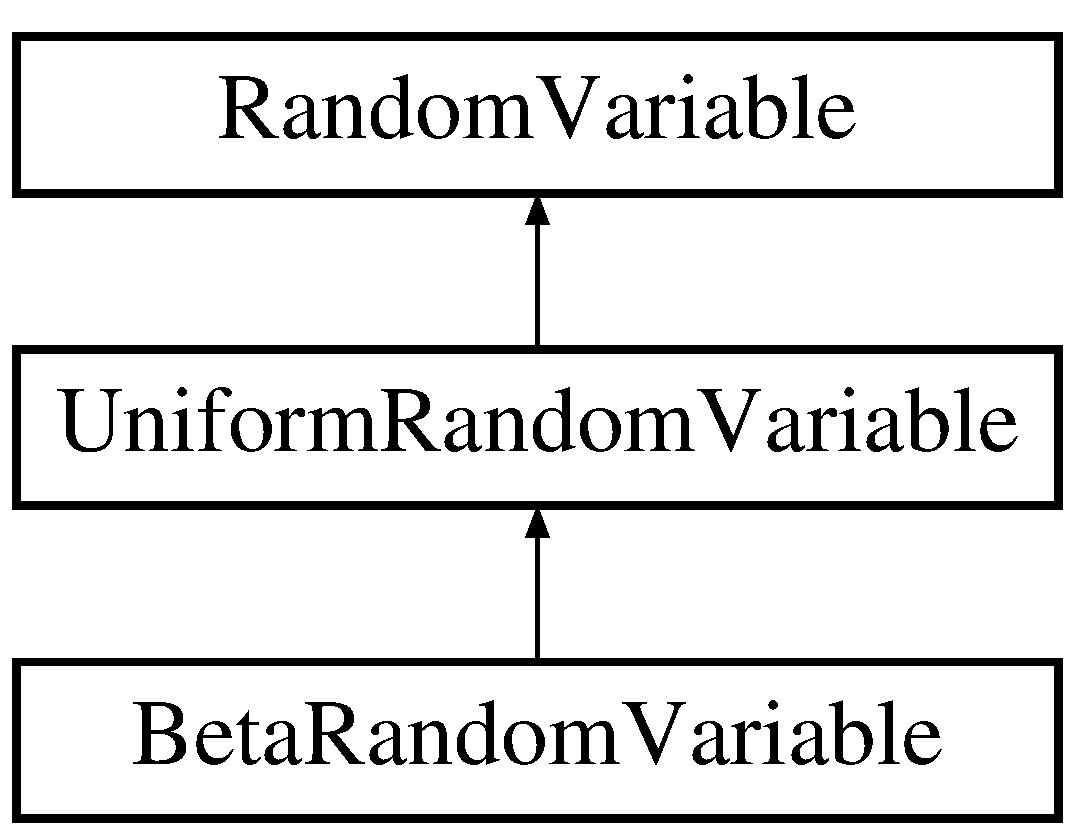
\includegraphics[height=3.000000cm]{classPecos_1_1BetaRandomVariable}
\end{center}
\end{figure}
\subsection*{Public Member Functions}
\begin{DoxyCompactItemize}
\item 
\hyperlink{classPecos_1_1BetaRandomVariable_a7ea24ac2918a0373d5310545dbd6d920}{Beta\+Random\+Variable} ()\label{classPecos_1_1BetaRandomVariable_a7ea24ac2918a0373d5310545dbd6d920}

\begin{DoxyCompactList}\small\item\em default constructor \end{DoxyCompactList}\item 
\hyperlink{classPecos_1_1BetaRandomVariable_a8552ab690ca1a372638c545ff78a3c57}{Beta\+Random\+Variable} (Real alpha, Real beta, Real lwr, Real upr)\label{classPecos_1_1BetaRandomVariable_a8552ab690ca1a372638c545ff78a3c57}

\begin{DoxyCompactList}\small\item\em alternate constructor \end{DoxyCompactList}\item 
\hyperlink{classPecos_1_1BetaRandomVariable_a93506d9a622032552279d3746c2ec9ea}{$\sim$\+Beta\+Random\+Variable} ()\label{classPecos_1_1BetaRandomVariable_a93506d9a622032552279d3746c2ec9ea}

\begin{DoxyCompactList}\small\item\em destructor \end{DoxyCompactList}\item 
Real \hyperlink{classPecos_1_1BetaRandomVariable_addd564e7f4f314e12d38df74d845f0d8}{cdf} (Real x) const \label{classPecos_1_1BetaRandomVariable_addd564e7f4f314e12d38df74d845f0d8}

\begin{DoxyCompactList}\small\item\em return the cumulative distribution function value of the random variable at x \end{DoxyCompactList}\item 
Real \hyperlink{classPecos_1_1BetaRandomVariable_a23c3b599e7e4788a9a5e9e93c3dbaf4d}{ccdf} (Real x) const \label{classPecos_1_1BetaRandomVariable_a23c3b599e7e4788a9a5e9e93c3dbaf4d}

\begin{DoxyCompactList}\small\item\em return the complementary cumulative distribution function value of the random variable at x \end{DoxyCompactList}\item 
Real \hyperlink{classPecos_1_1BetaRandomVariable_a918a1aac05ca349ea5313eebcba46c3e}{inverse\+\_\+cdf} (Real p\+\_\+cdf) const \label{classPecos_1_1BetaRandomVariable_a918a1aac05ca349ea5313eebcba46c3e}

\begin{DoxyCompactList}\small\item\em return the x value corresponding to a cumulative probability \end{DoxyCompactList}\item 
Real \hyperlink{classPecos_1_1BetaRandomVariable_afda003a1f59ff6930902cd5c8601f49b}{inverse\+\_\+ccdf} (Real p\+\_\+ccdf) const \label{classPecos_1_1BetaRandomVariable_afda003a1f59ff6930902cd5c8601f49b}

\begin{DoxyCompactList}\small\item\em return the x value corresponding to a complementary cumulative probability \end{DoxyCompactList}\item 
Real \hyperlink{classPecos_1_1BetaRandomVariable_a8ec69265f428e17c1707133cb137a819}{pdf} (Real x) const \label{classPecos_1_1BetaRandomVariable_a8ec69265f428e17c1707133cb137a819}

\begin{DoxyCompactList}\small\item\em return the value of the random variable\textquotesingle{}s probability density function at x \end{DoxyCompactList}\item 
Real \hyperlink{classPecos_1_1BetaRandomVariable_aaa7ca3718abc034be7629af5594efca0}{pdf\+\_\+gradient} (Real x) const \label{classPecos_1_1BetaRandomVariable_aaa7ca3718abc034be7629af5594efca0}

\begin{DoxyCompactList}\small\item\em return the gradient of the random variable\textquotesingle{}s probability density function at x \end{DoxyCompactList}\item 
Real \hyperlink{classPecos_1_1BetaRandomVariable_a514a0abe97269ac6e003f43683d9137e}{pdf\+\_\+hessian} (Real x) const \label{classPecos_1_1BetaRandomVariable_a514a0abe97269ac6e003f43683d9137e}

\begin{DoxyCompactList}\small\item\em return the hessian of the random variable\textquotesingle{}s probability density function at x \end{DoxyCompactList}\item 
Real \hyperlink{classPecos_1_1BetaRandomVariable_a6e2b6b6f13eedb2eb1ef3bc455a06392}{log\+\_\+pdf} (Real x) const \label{classPecos_1_1BetaRandomVariable_a6e2b6b6f13eedb2eb1ef3bc455a06392}

\begin{DoxyCompactList}\small\item\em return the value of the natural log of the random variable\textquotesingle{}s probability density function at x (useful for calculations of log density in Bayesian methods) \end{DoxyCompactList}\item 
Real \hyperlink{classPecos_1_1BetaRandomVariable_a5ccc16c04690f0c501f44c1ffae2bbd1}{log\+\_\+pdf\+\_\+gradient} (Real x) const \label{classPecos_1_1BetaRandomVariable_a5ccc16c04690f0c501f44c1ffae2bbd1}

\begin{DoxyCompactList}\small\item\em return the gradient of the natural log of the random variable\textquotesingle{}s probability density function at x (useful for defining M\+C\+MC proposal distributions in Bayesian methods) \end{DoxyCompactList}\item 
Real \hyperlink{classPecos_1_1BetaRandomVariable_a7b43f26f0f2bcdfef15d87e1f9399b33}{log\+\_\+pdf\+\_\+hessian} (Real x) const \label{classPecos_1_1BetaRandomVariable_a7b43f26f0f2bcdfef15d87e1f9399b33}

\begin{DoxyCompactList}\small\item\em return the Hessian of the natural log of the random variable\textquotesingle{}s probability density function at x (useful for defining M\+C\+MC proposal distributions in Bayesian methods) \end{DoxyCompactList}\item 
Real \hyperlink{classPecos_1_1BetaRandomVariable_acffcd338a207168a147fffe0778ccf3c}{inverse\+\_\+standard\+\_\+cdf} (Real p\+\_\+cdf) const \label{classPecos_1_1BetaRandomVariable_acffcd338a207168a147fffe0778ccf3c}

\begin{DoxyCompactList}\small\item\em return the x value for a standardized probability distribution corresponding to a cumulative probability \end{DoxyCompactList}\item 
Real \hyperlink{classPecos_1_1BetaRandomVariable_a206a02581b82f44be4a5321488a12daa}{standard\+\_\+pdf} (Real z) const \label{classPecos_1_1BetaRandomVariable_a206a02581b82f44be4a5321488a12daa}

\begin{DoxyCompactList}\small\item\em return the value of a standardized random variable\textquotesingle{}s probability density function at x \end{DoxyCompactList}\item 
Real \hyperlink{classPecos_1_1BetaRandomVariable_a1eb7deb350fc38d35e32ba7d0b96c464}{log\+\_\+standard\+\_\+pdf} (Real z) const \label{classPecos_1_1BetaRandomVariable_a1eb7deb350fc38d35e32ba7d0b96c464}

\begin{DoxyCompactList}\small\item\em return the natural log of a standardized random variable\textquotesingle{}s probability density function at x (useful for calculations of log density in Bayesian methods) \end{DoxyCompactList}\item 
Real \hyperlink{classPecos_1_1BetaRandomVariable_a73ea75d51f5415f600bebbca4a9628b7}{log\+\_\+standard\+\_\+pdf\+\_\+gradient} (Real z) const \label{classPecos_1_1BetaRandomVariable_a73ea75d51f5415f600bebbca4a9628b7}

\begin{DoxyCompactList}\small\item\em return the gradient of the natural log of a standardized random variable\textquotesingle{}s probability density function at x (useful for calculations of log density in Bayesian methods) \end{DoxyCompactList}\item 
Real \hyperlink{classPecos_1_1BetaRandomVariable_acf89562740c674e54901e97817f56b69}{log\+\_\+standard\+\_\+pdf\+\_\+hessian} (Real z) const \label{classPecos_1_1BetaRandomVariable_acf89562740c674e54901e97817f56b69}

\begin{DoxyCompactList}\small\item\em return the Hessian of the natural log of a standardized random variable\textquotesingle{}s probability density function at x (useful for calculations of log density in Bayesian methods) \end{DoxyCompactList}\item 
Real \hyperlink{classPecos_1_1BetaRandomVariable_aa891dab1ae9a225f493e3a0e5032b778}{parameter} (short dist\+\_\+param) const \label{classPecos_1_1BetaRandomVariable_aa891dab1ae9a225f493e3a0e5032b778}

\begin{DoxyCompactList}\small\item\em return the value of the named distribution parameter \end{DoxyCompactList}\item 
void \hyperlink{classPecos_1_1BetaRandomVariable_ae8e123224f588aee676d5d56d5ca900d}{parameter} (short dist\+\_\+param, Real val)\label{classPecos_1_1BetaRandomVariable_ae8e123224f588aee676d5d56d5ca900d}

\begin{DoxyCompactList}\small\item\em update the value of the named distribution parameter \end{DoxyCompactList}\item 
Real \hyperlink{classPecos_1_1BetaRandomVariable_a962ffe5a3593be370d5c883365c060f4}{mean} () const \label{classPecos_1_1BetaRandomVariable_a962ffe5a3593be370d5c883365c060f4}

\begin{DoxyCompactList}\small\item\em return the distribution mean \end{DoxyCompactList}\item 
Real \hyperlink{classPecos_1_1BetaRandomVariable_ae1fff19ce29a79d657043a598523635d}{median} () const \label{classPecos_1_1BetaRandomVariable_ae1fff19ce29a79d657043a598523635d}

\begin{DoxyCompactList}\small\item\em return the distribution mode \end{DoxyCompactList}\item 
Real \hyperlink{classPecos_1_1BetaRandomVariable_a72d3d6926edd929cb3f8e12baa655f70}{mode} () const \label{classPecos_1_1BetaRandomVariable_a72d3d6926edd929cb3f8e12baa655f70}

\begin{DoxyCompactList}\small\item\em return the distribution mode \end{DoxyCompactList}\item 
Real \hyperlink{classPecos_1_1BetaRandomVariable_a6a4ed9624d511f8a4e4f509c82cb0706}{standard\+\_\+deviation} () const \label{classPecos_1_1BetaRandomVariable_a6a4ed9624d511f8a4e4f509c82cb0706}

\begin{DoxyCompactList}\small\item\em return the distribution variance \end{DoxyCompactList}\item 
Real \hyperlink{classPecos_1_1BetaRandomVariable_a4b8b05b2a9af92dad9cc304c2925a4eb}{variance} () const \label{classPecos_1_1BetaRandomVariable_a4b8b05b2a9af92dad9cc304c2925a4eb}

\begin{DoxyCompactList}\small\item\em return the distribution variance \end{DoxyCompactList}\item 
Real \hyperlink{classPecos_1_1BetaRandomVariable_af889af8adfb262c9b74f573b2a9ffc99}{dx\+\_\+ds} (short dist\+\_\+param, short u\+\_\+type, Real x, Real z) const 
\item 
Real \hyperlink{classPecos_1_1BetaRandomVariable_af6b5fc528523180bed5fc3008dcea205}{dz\+\_\+ds\+\_\+factor} (short u\+\_\+type, Real x, Real z) const 
\item 
void {\bfseries update} (Real alpha, Real beta, Real lwr, Real upr)\label{classPecos_1_1BetaRandomVariable_a3c80355aecb28e989e2bc0124f5eff16}

\end{DoxyCompactItemize}
\subsection*{Static Public Member Functions}
\begin{DoxyCompactItemize}
\item 
static Real {\bfseries std\+\_\+pdf} (Real x, Real alpha, Real beta)\label{classPecos_1_1BetaRandomVariable_a6e32e04360dd9ebde5708412529b4c90}

\item 
static Real {\bfseries std\+\_\+cdf} (Real x, Real alpha, Real beta)\label{classPecos_1_1BetaRandomVariable_a80475bc6525448bf737486a6f2566116}

\item 
static Real {\bfseries inverse\+\_\+std\+\_\+cdf} (Real \hyperlink{classPecos_1_1BetaRandomVariable_addd564e7f4f314e12d38df74d845f0d8}{cdf}, Real alpha, Real beta)\label{classPecos_1_1BetaRandomVariable_ac31749979131683659e37e1eb7841e4e}

\item 
static Real {\bfseries pdf} (Real x, Real alpha, Real beta, Real lwr, Real upr)\label{classPecos_1_1BetaRandomVariable_adcf2fd976567fb799f3136d18185bf2b}

\item 
static Real {\bfseries cdf} (Real x, Real alpha, Real beta, Real lwr, Real upr)\label{classPecos_1_1BetaRandomVariable_a8abd3c476eb56d9e00bcaeb5f04dd045}

\item 
static void {\bfseries moments\+\_\+from\+\_\+params} (Real alpha, Real beta, Real lwr, Real upr, Real \&\hyperlink{classPecos_1_1BetaRandomVariable_a962ffe5a3593be370d5c883365c060f4}{mean}, Real \&std\+\_\+dev)\label{classPecos_1_1BetaRandomVariable_ab1648d3674b3fa004b33600fe5c59fad}

\end{DoxyCompactItemize}
\subsection*{Protected Member Functions}
\begin{DoxyCompactItemize}
\item 
void \hyperlink{classPecos_1_1BetaRandomVariable_aaa6750cbee2245416a6eeeac58d4405a}{update\+\_\+boost} ()\label{classPecos_1_1BetaRandomVariable_aaa6750cbee2245416a6eeeac58d4405a}

\begin{DoxyCompactList}\small\item\em create a new beta\+Dist instance \end{DoxyCompactList}\end{DoxyCompactItemize}
\subsection*{Protected Attributes}
\begin{DoxyCompactItemize}
\item 
Real \hyperlink{classPecos_1_1BetaRandomVariable_aa48da95b9214d9cf933e1d4625e32e84}{alpha\+Stat}\label{classPecos_1_1BetaRandomVariable_aa48da95b9214d9cf933e1d4625e32e84}

\begin{DoxyCompactList}\small\item\em alpha parameter of beta random variable (statistical P\+DF convention; differs from Jacobi polynomial convention) \end{DoxyCompactList}\item 
Real \hyperlink{classPecos_1_1BetaRandomVariable_a838d220373c3360feec45e853b0daaac}{beta\+Stat}\label{classPecos_1_1BetaRandomVariable_a838d220373c3360feec45e853b0daaac}

\begin{DoxyCompactList}\small\item\em beta parameter of beta random variable (statistical P\+DF convention; differs from Jacobi polynomial convention) \end{DoxyCompactList}\item 
beta\+\_\+dist $\ast$ \hyperlink{classPecos_1_1BetaRandomVariable_a09cc5637bd2b75284abc85d89473e3a5}{beta\+Dist}\label{classPecos_1_1BetaRandomVariable_a09cc5637bd2b75284abc85d89473e3a5}

\begin{DoxyCompactList}\small\item\em pointer to the Boost beta\+\_\+distribution instance \end{DoxyCompactList}\end{DoxyCompactItemize}


\subsection{Detailed Description}
Derived random variable class for beta random variables. 

Manages alpha and beta and inherits bounds. See Haldar and Mahadevan, p. 72. 

\subsection{Member Function Documentation}
\index{Pecos\+::\+Beta\+Random\+Variable@{Pecos\+::\+Beta\+Random\+Variable}!dx\+\_\+ds@{dx\+\_\+ds}}
\index{dx\+\_\+ds@{dx\+\_\+ds}!Pecos\+::\+Beta\+Random\+Variable@{Pecos\+::\+Beta\+Random\+Variable}}
\subsubsection[{\texorpdfstring{dx\+\_\+ds(short dist\+\_\+param, short u\+\_\+type, Real x, Real z) const }{dx_ds(short dist_param, short u_type, Real x, Real z) const }}]{\setlength{\rightskip}{0pt plus 5cm}Real dx\+\_\+ds (
\begin{DoxyParamCaption}
\item[{short}]{dist\+\_\+param, }
\item[{short}]{u\+\_\+type, }
\item[{Real}]{x, }
\item[{Real}]{z}
\end{DoxyParamCaption}
) const\hspace{0.3cm}{\ttfamily [inline]}, {\ttfamily [virtual]}}\label{classPecos_1_1BetaRandomVariable_af889af8adfb262c9b74f573b2a9ffc99}
dx/ds is derived by differentiating \hyperlink{classPecos_1_1NatafTransformation_a5feeecf846fc017c5a28eccb4e955dc1}{Nataf\+Transformation\+::trans\+\_\+\+Z\+\_\+to\+\_\+\+X()} with respect to distribution parameter s. dz/ds is zero if uncorrelated, while \hyperlink{classPecos_1_1BetaRandomVariable_af6b5fc528523180bed5fc3008dcea205}{dz\+\_\+ds\+\_\+factor()} manages contributions in the correlated case. 

Reimplemented from \hyperlink{classPecos_1_1RandomVariable_af889af8adfb262c9b74f573b2a9ffc99}{Random\+Variable}.



Referenced by Beta\+Random\+Variable\+::variance().

\index{Pecos\+::\+Beta\+Random\+Variable@{Pecos\+::\+Beta\+Random\+Variable}!dz\+\_\+ds\+\_\+factor@{dz\+\_\+ds\+\_\+factor}}
\index{dz\+\_\+ds\+\_\+factor@{dz\+\_\+ds\+\_\+factor}!Pecos\+::\+Beta\+Random\+Variable@{Pecos\+::\+Beta\+Random\+Variable}}
\subsubsection[{\texorpdfstring{dz\+\_\+ds\+\_\+factor(short u\+\_\+type, Real x, Real z) const }{dz_ds_factor(short u_type, Real x, Real z) const }}]{\setlength{\rightskip}{0pt plus 5cm}Real dz\+\_\+ds\+\_\+factor (
\begin{DoxyParamCaption}
\item[{short}]{u\+\_\+type, }
\item[{Real}]{x, }
\item[{Real}]{z}
\end{DoxyParamCaption}
) const\hspace{0.3cm}{\ttfamily [inline]}, {\ttfamily [virtual]}}\label{classPecos_1_1BetaRandomVariable_af6b5fc528523180bed5fc3008dcea205}
dx/ds is derived by differentiating \hyperlink{classPecos_1_1NatafTransformation_a5feeecf846fc017c5a28eccb4e955dc1}{Nataf\+Transformation\+::trans\+\_\+\+Z\+\_\+to\+\_\+\+X()} with respect to distribution parameter s. For the uncorrelated case, u and z are constants. For the correlated case, u is a constant, but z(s) = L(s) u due to Nataf dependence on s and dz/ds = d\+L/ds u. 

Reimplemented from \hyperlink{classPecos_1_1RandomVariable_af6b5fc528523180bed5fc3008dcea205}{Random\+Variable}.



References Uniform\+Random\+Variable\+::lower\+Bnd, and Uniform\+Random\+Variable\+::upper\+Bnd.



The documentation for this class was generated from the following file\+:\begin{DoxyCompactItemize}
\item 
Beta\+Random\+Variable.\+hpp\end{DoxyCompactItemize}

\section{Binomial\+Random\+Variable Class Reference}
\label{classPecos_1_1BinomialRandomVariable}\index{Binomial\+Random\+Variable@{Binomial\+Random\+Variable}}


Derived random variable class for binomial random variables.  


Inheritance diagram for Binomial\+Random\+Variable\+:\begin{figure}[H]
\begin{center}
\leavevmode
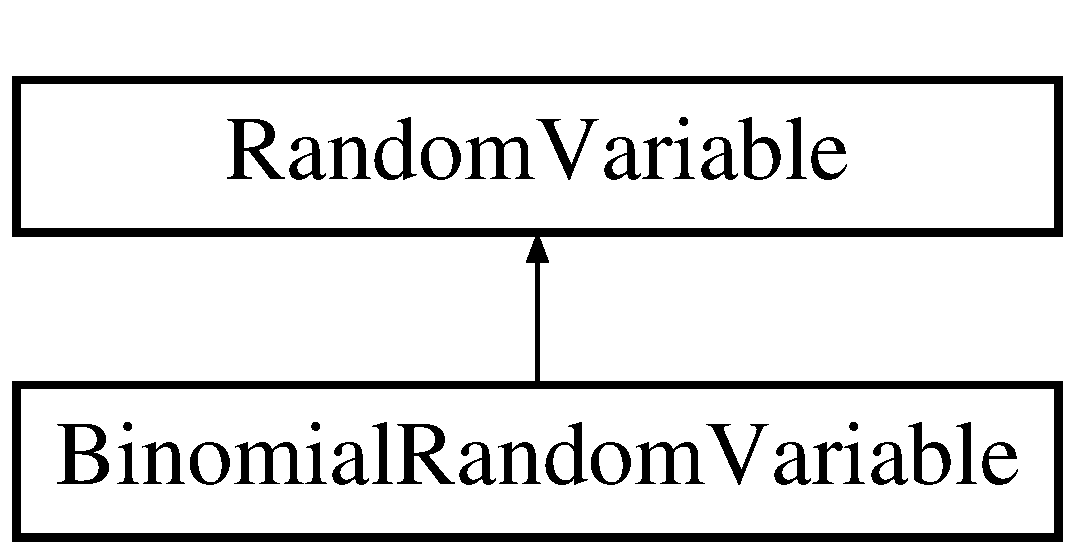
\includegraphics[height=2.000000cm]{classPecos_1_1BinomialRandomVariable}
\end{center}
\end{figure}
\subsection*{Public Member Functions}
\begin{DoxyCompactItemize}
\item 
\hyperlink{classPecos_1_1BinomialRandomVariable_a218da5f5afff8a7a223cdbd2263cf3bd}{Binomial\+Random\+Variable} ()\label{classPecos_1_1BinomialRandomVariable_a218da5f5afff8a7a223cdbd2263cf3bd}

\begin{DoxyCompactList}\small\item\em default constructor \end{DoxyCompactList}\item 
\hyperlink{classPecos_1_1BinomialRandomVariable_a4ec1ac0122a9d28492dc7763ca309db8}{Binomial\+Random\+Variable} (unsigned int num\+\_\+trials, Real prob\+\_\+per\+\_\+trial)\label{classPecos_1_1BinomialRandomVariable_a4ec1ac0122a9d28492dc7763ca309db8}

\begin{DoxyCompactList}\small\item\em alternate constructor \end{DoxyCompactList}\item 
\hyperlink{classPecos_1_1BinomialRandomVariable_aec4d48ee5c7eef39b1dfd29bb9a17968}{$\sim$\+Binomial\+Random\+Variable} ()\label{classPecos_1_1BinomialRandomVariable_aec4d48ee5c7eef39b1dfd29bb9a17968}

\begin{DoxyCompactList}\small\item\em destructor \end{DoxyCompactList}\item 
Real \hyperlink{classPecos_1_1BinomialRandomVariable_addd564e7f4f314e12d38df74d845f0d8}{cdf} (Real x) const \label{classPecos_1_1BinomialRandomVariable_addd564e7f4f314e12d38df74d845f0d8}

\begin{DoxyCompactList}\small\item\em return the cumulative distribution function value of the random variable at x \end{DoxyCompactList}\item 
Real \hyperlink{classPecos_1_1BinomialRandomVariable_a23c3b599e7e4788a9a5e9e93c3dbaf4d}{ccdf} (Real x) const \label{classPecos_1_1BinomialRandomVariable_a23c3b599e7e4788a9a5e9e93c3dbaf4d}

\begin{DoxyCompactList}\small\item\em return the complementary cumulative distribution function value of the random variable at x \end{DoxyCompactList}\item 
Real \hyperlink{classPecos_1_1BinomialRandomVariable_a918a1aac05ca349ea5313eebcba46c3e}{inverse\+\_\+cdf} (Real p\+\_\+cdf) const \label{classPecos_1_1BinomialRandomVariable_a918a1aac05ca349ea5313eebcba46c3e}

\begin{DoxyCompactList}\small\item\em return the x value corresponding to a cumulative probability \end{DoxyCompactList}\item 
Real \hyperlink{classPecos_1_1BinomialRandomVariable_afda003a1f59ff6930902cd5c8601f49b}{inverse\+\_\+ccdf} (Real p\+\_\+ccdf) const \label{classPecos_1_1BinomialRandomVariable_afda003a1f59ff6930902cd5c8601f49b}

\begin{DoxyCompactList}\small\item\em return the x value corresponding to a complementary cumulative probability \end{DoxyCompactList}\item 
Real \hyperlink{classPecos_1_1BinomialRandomVariable_a8ec69265f428e17c1707133cb137a819}{pdf} (Real x) const \label{classPecos_1_1BinomialRandomVariable_a8ec69265f428e17c1707133cb137a819}

\begin{DoxyCompactList}\small\item\em return the value of the random variable\textquotesingle{}s probability density function at x \end{DoxyCompactList}\item 
Real \hyperlink{classPecos_1_1BinomialRandomVariable_aa891dab1ae9a225f493e3a0e5032b778}{parameter} (short dist\+\_\+param) const \label{classPecos_1_1BinomialRandomVariable_aa891dab1ae9a225f493e3a0e5032b778}

\begin{DoxyCompactList}\small\item\em return the value of the named distribution parameter \end{DoxyCompactList}\item 
void \hyperlink{classPecos_1_1BinomialRandomVariable_ae8e123224f588aee676d5d56d5ca900d}{parameter} (short dist\+\_\+param, Real val)\label{classPecos_1_1BinomialRandomVariable_ae8e123224f588aee676d5d56d5ca900d}

\begin{DoxyCompactList}\small\item\em update the value of the named distribution parameter \end{DoxyCompactList}\item 
Real \hyperlink{classPecos_1_1BinomialRandomVariable_a962ffe5a3593be370d5c883365c060f4}{mean} () const \label{classPecos_1_1BinomialRandomVariable_a962ffe5a3593be370d5c883365c060f4}

\begin{DoxyCompactList}\small\item\em return the distribution mean \end{DoxyCompactList}\item 
Real \hyperlink{classPecos_1_1BinomialRandomVariable_ae1fff19ce29a79d657043a598523635d}{median} () const \label{classPecos_1_1BinomialRandomVariable_ae1fff19ce29a79d657043a598523635d}

\begin{DoxyCompactList}\small\item\em return the distribution mode \end{DoxyCompactList}\item 
Real \hyperlink{classPecos_1_1BinomialRandomVariable_a72d3d6926edd929cb3f8e12baa655f70}{mode} () const \label{classPecos_1_1BinomialRandomVariable_a72d3d6926edd929cb3f8e12baa655f70}

\begin{DoxyCompactList}\small\item\em return the distribution mode \end{DoxyCompactList}\item 
Real \hyperlink{classPecos_1_1BinomialRandomVariable_a6a4ed9624d511f8a4e4f509c82cb0706}{standard\+\_\+deviation} () const \label{classPecos_1_1BinomialRandomVariable_a6a4ed9624d511f8a4e4f509c82cb0706}

\begin{DoxyCompactList}\small\item\em return the distribution variance \end{DoxyCompactList}\item 
Real \hyperlink{classPecos_1_1BinomialRandomVariable_a4b8b05b2a9af92dad9cc304c2925a4eb}{variance} () const \label{classPecos_1_1BinomialRandomVariable_a4b8b05b2a9af92dad9cc304c2925a4eb}

\begin{DoxyCompactList}\small\item\em return the distribution variance \end{DoxyCompactList}\item 
Real\+Real\+Pair \hyperlink{classPecos_1_1BinomialRandomVariable_a4bdb95a8fa5fffaa0de5102f56963cf2}{bounds} () const \label{classPecos_1_1BinomialRandomVariable_a4bdb95a8fa5fffaa0de5102f56963cf2}

\begin{DoxyCompactList}\small\item\em return the distribution lower and upper bounds as a pair \end{DoxyCompactList}\item 
void {\bfseries update} (unsigned int num\+\_\+trials, Real prob\+\_\+per\+\_\+trial)\label{classPecos_1_1BinomialRandomVariable_a87163ad5a4f469108f079d0e8c6c2cb8}

\end{DoxyCompactItemize}
\subsection*{Static Public Member Functions}
\begin{DoxyCompactItemize}
\item 
static Real {\bfseries pdf} (Real x, unsigned int num\+\_\+trials, Real prob\+\_\+per\+\_\+trial)\label{classPecos_1_1BinomialRandomVariable_a2886ea0e23e30bbbc464565416eb6614}

\item 
static Real {\bfseries cdf} (Real x, unsigned int num\+\_\+trials, Real prob\+\_\+per\+\_\+trial)\label{classPecos_1_1BinomialRandomVariable_a630e535fde694c4b082312a4fd082f3d}

\item 
static void {\bfseries moments\+\_\+from\+\_\+params} (unsigned int num\+\_\+trials, Real prob\+\_\+per\+\_\+trial, Real \&\hyperlink{classPecos_1_1BinomialRandomVariable_a962ffe5a3593be370d5c883365c060f4}{mean}, Real \&std\+\_\+dev)\label{classPecos_1_1BinomialRandomVariable_ab5304d2842c683e30818638d9e7150ba}

\end{DoxyCompactItemize}
\subsection*{Protected Member Functions}
\begin{DoxyCompactItemize}
\item 
void \hyperlink{classPecos_1_1BinomialRandomVariable_aaa6750cbee2245416a6eeeac58d4405a}{update\+\_\+boost} ()\label{classPecos_1_1BinomialRandomVariable_aaa6750cbee2245416a6eeeac58d4405a}

\begin{DoxyCompactList}\small\item\em create a new binomial\+Dist instance \end{DoxyCompactList}\end{DoxyCompactItemize}
\subsection*{Protected Attributes}
\begin{DoxyCompactItemize}
\item 
unsigned int \hyperlink{classPecos_1_1BinomialRandomVariable_ae7284c5049f25d6872f8fbe98c855e0c}{num\+Trials}\label{classPecos_1_1BinomialRandomVariable_ae7284c5049f25d6872f8fbe98c855e0c}

\begin{DoxyCompactList}\small\item\em n parameter of binomial random variable \end{DoxyCompactList}\item 
Real \hyperlink{classPecos_1_1BinomialRandomVariable_a034cce918fd6c1433e74212387527794}{prob\+Per\+Trial}\label{classPecos_1_1BinomialRandomVariable_a034cce918fd6c1433e74212387527794}

\begin{DoxyCompactList}\small\item\em p parameter of binomial random variable \end{DoxyCompactList}\item 
binomial\+\_\+dist $\ast$ \hyperlink{classPecos_1_1BinomialRandomVariable_ad960997d630c90336be0ddf0deda3cd0}{binomial\+Dist}\label{classPecos_1_1BinomialRandomVariable_ad960997d630c90336be0ddf0deda3cd0}

\begin{DoxyCompactList}\small\item\em pointer to the Boost binomial\+\_\+distribution instance \end{DoxyCompactList}\end{DoxyCompactItemize}


\subsection{Detailed Description}
Derived random variable class for binomial random variables. 

Manages num\+Trials and prob\+Per\+Trial parameters. 

The documentation for this class was generated from the following file\+:\begin{DoxyCompactItemize}
\item 
Binomial\+Random\+Variable.\+hpp\end{DoxyCompactItemize}

\section{Boost\+R\+N\+G\+\_\+\+Monostate Class Reference}
\label{classPecos_1_1BoostRNG__Monostate}\index{Boost\+R\+N\+G\+\_\+\+Monostate@{Boost\+R\+N\+G\+\_\+\+Monostate}}
\subsection*{Static Public Member Functions}
\begin{DoxyCompactItemize}
\item 
static void \hyperlink{classPecos_1_1BoostRNG__Monostate_a30a665dc3d2e81cf2110f6a362f10481}{seed} (unsigned int rng\+\_\+seed)\label{classPecos_1_1BoostRNG__Monostate_a30a665dc3d2e81cf2110f6a362f10481}

\begin{DoxyCompactList}\small\item\em set random\+Seed \end{DoxyCompactList}\item 
static unsigned int \hyperlink{classPecos_1_1BoostRNG__Monostate_a38dd7ac12fd0a21d3e5e940c193c62fa}{seed} ()\label{classPecos_1_1BoostRNG__Monostate_a38dd7ac12fd0a21d3e5e940c193c62fa}

\begin{DoxyCompactList}\small\item\em return random\+Seed \end{DoxyCompactList}\item 
static Real {\bfseries mt19937} ()\label{classPecos_1_1BoostRNG__Monostate_a310d5b8210e26a75ac903d05a8810df6}

\end{DoxyCompactItemize}
\subsection*{Static Public Attributes}
\begin{DoxyCompactItemize}
\item 
static Rfunc \hyperlink{classPecos_1_1BoostRNG__Monostate_a471db23ae67e284b64b62724ee6e5fd6}{random\+Num} = Boost\+R\+N\+G\+\_\+\+Monostate\+::mt19937\label{classPecos_1_1BoostRNG__Monostate_a471db23ae67e284b64b62724ee6e5fd6}

\begin{DoxyCompactList}\small\item\em Cached function pointers. \end{DoxyCompactList}\item 
static Rfunc {\bfseries random\+Num2} = Boost\+R\+N\+G\+\_\+\+Monostate\+::mt19937\label{classPecos_1_1BoostRNG__Monostate_af70eaa38bec1d222adab06c337805431}

\end{DoxyCompactItemize}
\subsection*{Static Private Attributes}
\begin{DoxyCompactItemize}
\item 
static unsigned int {\bfseries rng\+Seed}\label{classPecos_1_1BoostRNG__Monostate_a9411e7020b48b5f4bda9454ebd58dac2}

\item 
static boost\+::mt19937 {\bfseries rnum\+Generator}\label{classPecos_1_1BoostRNG__Monostate_ac1eae1eea544fd3712ae5a8d62724ddf}

\item 
static boost\+::uniform\+\_\+real {\bfseries uni\+Dist}\label{classPecos_1_1BoostRNG__Monostate_aeb12dfc2fa20445c0bc97650b4b91877}

\item 
static boost\+::variate\+\_\+generator$<$ boost\+::mt19937 \&, boost\+::uniform\+\_\+real$<$$>$ $>$ {\bfseries uni\+MT}\label{classPecos_1_1BoostRNG__Monostate_a5ec148ef3f4bea4dfdfdf3f24e2094c7}

\end{DoxyCompactItemize}


\subsection{Detailed Description}
The monostate Boost\+R\+NG class provides static pointers random\+Num and random\+Num2 that at runtime will either point to Boost\+R\+N\+G\+\_\+\+Monostate\+::mt19937, or be overridden to point to defaultnum1 / defaultrnum2. At construct time they point to the \hyperlink{classPecos_1_1BoostRNG__Monostate}{Boost\+R\+N\+G\+\_\+\+Monostate} generators. 

The documentation for this class was generated from the following file\+:\begin{DoxyCompactItemize}
\item 
Boost\+R\+N\+G\+\_\+\+Monostate.\+hpp\end{DoxyCompactItemize}

\section{Bounded\+Lognormal\+Random\+Variable Class Reference}
\label{classPecos_1_1BoundedLognormalRandomVariable}\index{Bounded\+Lognormal\+Random\+Variable@{Bounded\+Lognormal\+Random\+Variable}}


Derived random variable class for bounded lognormal random variables.  


Inheritance diagram for Bounded\+Lognormal\+Random\+Variable\+:\begin{figure}[H]
\begin{center}
\leavevmode
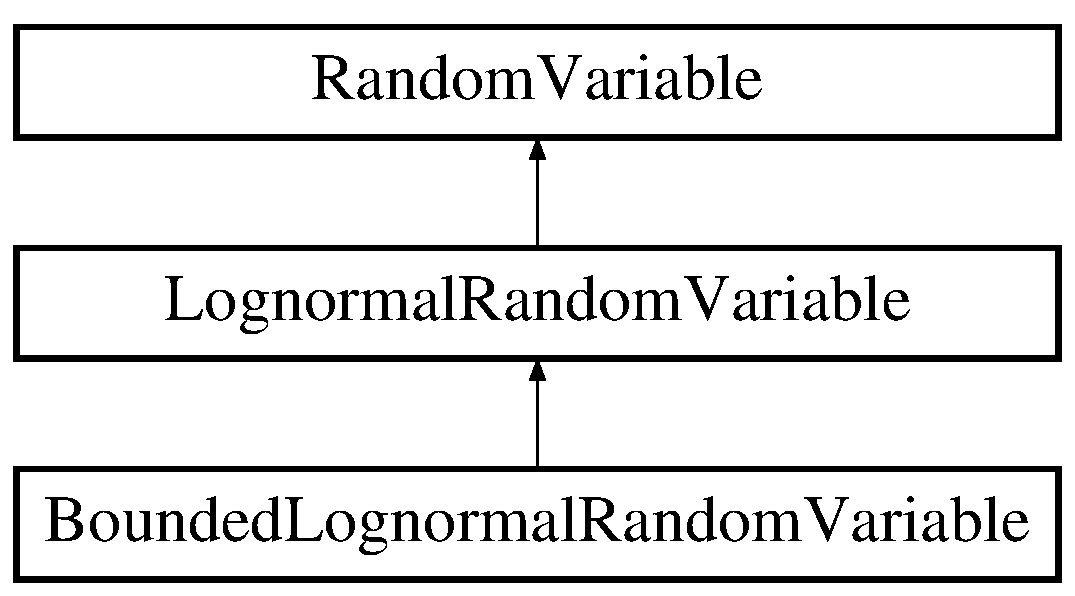
\includegraphics[height=3.000000cm]{classPecos_1_1BoundedLognormalRandomVariable}
\end{center}
\end{figure}
\subsection*{Public Member Functions}
\begin{DoxyCompactItemize}
\item 
\hyperlink{classPecos_1_1BoundedLognormalRandomVariable_a474166c30b501daa45b7b752fb4918b5}{Bounded\+Lognormal\+Random\+Variable} ()\label{classPecos_1_1BoundedLognormalRandomVariable_a474166c30b501daa45b7b752fb4918b5}

\begin{DoxyCompactList}\small\item\em default constructor \end{DoxyCompactList}\item 
\hyperlink{classPecos_1_1BoundedLognormalRandomVariable_af72e9e277a3430a2c33f131bdfb0e23c}{Bounded\+Lognormal\+Random\+Variable} (Real lambda, Real zeta, Real lwr, Real upr)\label{classPecos_1_1BoundedLognormalRandomVariable_af72e9e277a3430a2c33f131bdfb0e23c}

\begin{DoxyCompactList}\small\item\em alternate constructor \end{DoxyCompactList}\item 
\hyperlink{classPecos_1_1BoundedLognormalRandomVariable_a807f5f719688a9656c0fdaec5ae3341b}{$\sim$\+Bounded\+Lognormal\+Random\+Variable} ()\label{classPecos_1_1BoundedLognormalRandomVariable_a807f5f719688a9656c0fdaec5ae3341b}

\begin{DoxyCompactList}\small\item\em destructor \end{DoxyCompactList}\item 
Real \hyperlink{classPecos_1_1BoundedLognormalRandomVariable_addd564e7f4f314e12d38df74d845f0d8}{cdf} (Real x) const \label{classPecos_1_1BoundedLognormalRandomVariable_addd564e7f4f314e12d38df74d845f0d8}

\begin{DoxyCompactList}\small\item\em return the cumulative distribution function value of the random variable at x \end{DoxyCompactList}\item 
Real \hyperlink{classPecos_1_1BoundedLognormalRandomVariable_a23c3b599e7e4788a9a5e9e93c3dbaf4d}{ccdf} (Real x) const \label{classPecos_1_1BoundedLognormalRandomVariable_a23c3b599e7e4788a9a5e9e93c3dbaf4d}

\begin{DoxyCompactList}\small\item\em return the complementary cumulative distribution function value of the random variable at x \end{DoxyCompactList}\item 
Real \hyperlink{classPecos_1_1BoundedLognormalRandomVariable_a918a1aac05ca349ea5313eebcba46c3e}{inverse\+\_\+cdf} (Real p\+\_\+cdf) const \label{classPecos_1_1BoundedLognormalRandomVariable_a918a1aac05ca349ea5313eebcba46c3e}

\begin{DoxyCompactList}\small\item\em return the x value corresponding to a cumulative probability \end{DoxyCompactList}\item 
Real \hyperlink{classPecos_1_1BoundedLognormalRandomVariable_afda003a1f59ff6930902cd5c8601f49b}{inverse\+\_\+ccdf} (Real p\+\_\+ccdf) const \label{classPecos_1_1BoundedLognormalRandomVariable_afda003a1f59ff6930902cd5c8601f49b}

\begin{DoxyCompactList}\small\item\em return the x value corresponding to a complementary cumulative probability \end{DoxyCompactList}\item 
Real \hyperlink{classPecos_1_1BoundedLognormalRandomVariable_a8ec69265f428e17c1707133cb137a819}{pdf} (Real x) const \label{classPecos_1_1BoundedLognormalRandomVariable_a8ec69265f428e17c1707133cb137a819}

\begin{DoxyCompactList}\small\item\em return the value of the random variable\textquotesingle{}s probability density function at x \end{DoxyCompactList}\item 
Real \hyperlink{classPecos_1_1BoundedLognormalRandomVariable_a6e2b6b6f13eedb2eb1ef3bc455a06392}{log\+\_\+pdf} (Real x) const \label{classPecos_1_1BoundedLognormalRandomVariable_a6e2b6b6f13eedb2eb1ef3bc455a06392}

\begin{DoxyCompactList}\small\item\em return the value of the natural log of the random variable\textquotesingle{}s probability density function at x (useful for calculations of log density in Bayesian methods) \end{DoxyCompactList}\item 
Real \hyperlink{classPecos_1_1BoundedLognormalRandomVariable_a5ccc16c04690f0c501f44c1ffae2bbd1}{log\+\_\+pdf\+\_\+gradient} (Real x) const \label{classPecos_1_1BoundedLognormalRandomVariable_a5ccc16c04690f0c501f44c1ffae2bbd1}

\begin{DoxyCompactList}\small\item\em return the gradient of the natural log of the random variable\textquotesingle{}s probability density function at x (useful for defining M\+C\+MC proposal distributions in Bayesian methods) \end{DoxyCompactList}\item 
Real \hyperlink{classPecos_1_1BoundedLognormalRandomVariable_a7b43f26f0f2bcdfef15d87e1f9399b33}{log\+\_\+pdf\+\_\+hessian} (Real x) const \label{classPecos_1_1BoundedLognormalRandomVariable_a7b43f26f0f2bcdfef15d87e1f9399b33}

\begin{DoxyCompactList}\small\item\em return the Hessian of the natural log of the random variable\textquotesingle{}s probability density function at x (useful for defining M\+C\+MC proposal distributions in Bayesian methods) \end{DoxyCompactList}\item 
Real \hyperlink{classPecos_1_1BoundedLognormalRandomVariable_aa891dab1ae9a225f493e3a0e5032b778}{parameter} (short dist\+\_\+param) const \label{classPecos_1_1BoundedLognormalRandomVariable_aa891dab1ae9a225f493e3a0e5032b778}

\begin{DoxyCompactList}\small\item\em return the value of the named distribution parameter \end{DoxyCompactList}\item 
void \hyperlink{classPecos_1_1BoundedLognormalRandomVariable_ae8e123224f588aee676d5d56d5ca900d}{parameter} (short dist\+\_\+param, Real val)\label{classPecos_1_1BoundedLognormalRandomVariable_ae8e123224f588aee676d5d56d5ca900d}

\begin{DoxyCompactList}\small\item\em update the value of the named distribution parameter \end{DoxyCompactList}\item 
Real \hyperlink{classPecos_1_1BoundedLognormalRandomVariable_a962ffe5a3593be370d5c883365c060f4}{mean} () const \label{classPecos_1_1BoundedLognormalRandomVariable_a962ffe5a3593be370d5c883365c060f4}

\begin{DoxyCompactList}\small\item\em return the distribution mean \end{DoxyCompactList}\item 
Real \hyperlink{classPecos_1_1BoundedLognormalRandomVariable_ae1fff19ce29a79d657043a598523635d}{median} () const \label{classPecos_1_1BoundedLognormalRandomVariable_ae1fff19ce29a79d657043a598523635d}

\begin{DoxyCompactList}\small\item\em return the distribution mode \end{DoxyCompactList}\item 
Real \hyperlink{classPecos_1_1BoundedLognormalRandomVariable_a72d3d6926edd929cb3f8e12baa655f70}{mode} () const \label{classPecos_1_1BoundedLognormalRandomVariable_a72d3d6926edd929cb3f8e12baa655f70}

\begin{DoxyCompactList}\small\item\em return the distribution mode \end{DoxyCompactList}\item 
Real \hyperlink{classPecos_1_1BoundedLognormalRandomVariable_a6a4ed9624d511f8a4e4f509c82cb0706}{standard\+\_\+deviation} () const \label{classPecos_1_1BoundedLognormalRandomVariable_a6a4ed9624d511f8a4e4f509c82cb0706}

\begin{DoxyCompactList}\small\item\em return the distribution variance \end{DoxyCompactList}\item 
Real \hyperlink{classPecos_1_1BoundedLognormalRandomVariable_a4b8b05b2a9af92dad9cc304c2925a4eb}{variance} () const \label{classPecos_1_1BoundedLognormalRandomVariable_a4b8b05b2a9af92dad9cc304c2925a4eb}

\begin{DoxyCompactList}\small\item\em return the distribution variance \end{DoxyCompactList}\item 
Real\+Real\+Pair \hyperlink{classPecos_1_1BoundedLognormalRandomVariable_a80e9024c98c6105a5eace8601a91b3d3}{moments} () const 
\begin{DoxyCompactList}\small\item\em return the distribution mean and standard deviation as a pair \end{DoxyCompactList}\item 
Real\+Real\+Pair \hyperlink{classPecos_1_1BoundedLognormalRandomVariable_a4bdb95a8fa5fffaa0de5102f56963cf2}{bounds} () const \label{classPecos_1_1BoundedLognormalRandomVariable_a4bdb95a8fa5fffaa0de5102f56963cf2}

\begin{DoxyCompactList}\small\item\em return the distribution lower and upper bounds as a pair \end{DoxyCompactList}\item 
Real \hyperlink{classPecos_1_1BoundedLognormalRandomVariable_ae1cf1c07047d7ad9dbb899aa01138d54}{coefficient\+\_\+of\+\_\+variation} () const 
\begin{DoxyCompactList}\small\item\em compute the coefficient of variation (used to compute selected correlation warping factors); defined for semi-\/infinite distributions with nonzero mean (lognormal, exponential, gamma, frechet, weibull) \end{DoxyCompactList}\item 
Real \hyperlink{classPecos_1_1BoundedLognormalRandomVariable_af889af8adfb262c9b74f573b2a9ffc99}{dx\+\_\+ds} (short dist\+\_\+param, short u\+\_\+type, Real x, Real z) const 
\item 
Real \hyperlink{classPecos_1_1BoundedLognormalRandomVariable_af6b5fc528523180bed5fc3008dcea205}{dz\+\_\+ds\+\_\+factor} (short u\+\_\+type, Real x, Real z) const 
\item 
void {\bfseries update} (Real lambda, Real zeta, Real lwr, Real upr)\label{classPecos_1_1BoundedLognormalRandomVariable_a9c7ca27852bfe1675122029df010234b}

\end{DoxyCompactItemize}
\subsection*{Static Public Member Functions}
\begin{DoxyCompactItemize}
\item 
static Real {\bfseries pdf} (Real x, Real lambda, Real zeta, Real lwr, Real upr)\label{classPecos_1_1BoundedLognormalRandomVariable_aa24b8af7eee1d8dadf31167bd93a02b0}

\item 
static Real {\bfseries cdf} (Real x, Real lambda, Real zeta, Real lwr, Real upr)\label{classPecos_1_1BoundedLognormalRandomVariable_a7a57d35555a34b211c5f35fe8f0a1cfc}

\end{DoxyCompactItemize}
\subsection*{Protected Attributes}
\begin{DoxyCompactItemize}
\item 
Real \hyperlink{classPecos_1_1BoundedLognormalRandomVariable_a346dc528fe624cdf3ebb56fb9539f550}{lower\+Bnd}\label{classPecos_1_1BoundedLognormalRandomVariable_a346dc528fe624cdf3ebb56fb9539f550}

\begin{DoxyCompactList}\small\item\em lower bound of bounded\+\_\+lognormal random variable \end{DoxyCompactList}\item 
Real \hyperlink{classPecos_1_1BoundedLognormalRandomVariable_a671794a0fe385a29a595e98f44cde031}{upper\+Bnd}\label{classPecos_1_1BoundedLognormalRandomVariable_a671794a0fe385a29a595e98f44cde031}

\begin{DoxyCompactList}\small\item\em upper bound of bounded\+\_\+lognormal random variable \end{DoxyCompactList}\end{DoxyCompactItemize}
\subsection*{Additional Inherited Members}


\subsection{Detailed Description}
Derived random variable class for bounded lognormal random variables. 

Manages lower and upper bounds. 

\subsection{Member Function Documentation}
\index{Pecos\+::\+Bounded\+Lognormal\+Random\+Variable@{Pecos\+::\+Bounded\+Lognormal\+Random\+Variable}!moments@{moments}}
\index{moments@{moments}!Pecos\+::\+Bounded\+Lognormal\+Random\+Variable@{Pecos\+::\+Bounded\+Lognormal\+Random\+Variable}}
\subsubsection[{\texorpdfstring{moments() const }{moments() const }}]{\setlength{\rightskip}{0pt plus 5cm}Real\+Real\+Pair moments (
\begin{DoxyParamCaption}
{}
\end{DoxyParamCaption}
) const\hspace{0.3cm}{\ttfamily [inline]}, {\ttfamily [virtual]}}\label{classPecos_1_1BoundedLognormalRandomVariable_a80e9024c98c6105a5eace8601a91b3d3}


return the distribution mean and standard deviation as a pair 

default is only overridden when more efficient to compute together 

Reimplemented from \hyperlink{classPecos_1_1RandomVariable_a80e9024c98c6105a5eace8601a91b3d3}{Random\+Variable}.



References Lognormal\+Random\+Variable\+::ln\+Lambda, Lognormal\+Random\+Variable\+::ln\+Zeta, Bounded\+Lognormal\+Random\+Variable\+::lower\+Bnd, Lognormal\+Random\+Variable\+::mean(), Bounded\+Lognormal\+Random\+Variable\+::mean(), Normal\+Random\+Variable\+::std\+\_\+cdf(), and Bounded\+Lognormal\+Random\+Variable\+::upper\+Bnd.



Referenced by Bounded\+Lognormal\+Random\+Variable\+::coefficient\+\_\+of\+\_\+variation(), and Bounded\+Lognormal\+Random\+Variable\+::variance().

\index{Pecos\+::\+Bounded\+Lognormal\+Random\+Variable@{Pecos\+::\+Bounded\+Lognormal\+Random\+Variable}!coefficient\+\_\+of\+\_\+variation@{coefficient\+\_\+of\+\_\+variation}}
\index{coefficient\+\_\+of\+\_\+variation@{coefficient\+\_\+of\+\_\+variation}!Pecos\+::\+Bounded\+Lognormal\+Random\+Variable@{Pecos\+::\+Bounded\+Lognormal\+Random\+Variable}}
\subsubsection[{\texorpdfstring{coefficient\+\_\+of\+\_\+variation() const }{coefficient_of_variation() const }}]{\setlength{\rightskip}{0pt plus 5cm}Real coefficient\+\_\+of\+\_\+variation (
\begin{DoxyParamCaption}
{}
\end{DoxyParamCaption}
) const\hspace{0.3cm}{\ttfamily [inline]}, {\ttfamily [virtual]}}\label{classPecos_1_1BoundedLognormalRandomVariable_ae1cf1c07047d7ad9dbb899aa01138d54}


compute the coefficient of variation (used to compute selected correlation warping factors); defined for semi-\/infinite distributions with nonzero mean (lognormal, exponential, gamma, frechet, weibull) 

default is only overridden when more efficient to compute together 

Reimplemented from \hyperlink{classPecos_1_1RandomVariable_ae1cf1c07047d7ad9dbb899aa01138d54}{Random\+Variable}.



References Bounded\+Lognormal\+Random\+Variable\+::dx\+\_\+ds(), and Bounded\+Lognormal\+Random\+Variable\+::moments().

\index{Pecos\+::\+Bounded\+Lognormal\+Random\+Variable@{Pecos\+::\+Bounded\+Lognormal\+Random\+Variable}!dx\+\_\+ds@{dx\+\_\+ds}}
\index{dx\+\_\+ds@{dx\+\_\+ds}!Pecos\+::\+Bounded\+Lognormal\+Random\+Variable@{Pecos\+::\+Bounded\+Lognormal\+Random\+Variable}}
\subsubsection[{\texorpdfstring{dx\+\_\+ds(short dist\+\_\+param, short u\+\_\+type, Real x, Real z) const }{dx_ds(short dist_param, short u_type, Real x, Real z) const }}]{\setlength{\rightskip}{0pt plus 5cm}Real dx\+\_\+ds (
\begin{DoxyParamCaption}
\item[{short}]{dist\+\_\+param, }
\item[{short}]{u\+\_\+type, }
\item[{Real}]{x, }
\item[{Real}]{z}
\end{DoxyParamCaption}
) const\hspace{0.3cm}{\ttfamily [inline]}, {\ttfamily [virtual]}}\label{classPecos_1_1BoundedLognormalRandomVariable_af889af8adfb262c9b74f573b2a9ffc99}
dx/ds is derived by differentiating \hyperlink{classPecos_1_1NatafTransformation_a5feeecf846fc017c5a28eccb4e955dc1}{Nataf\+Transformation\+::trans\+\_\+\+Z\+\_\+to\+\_\+\+X()} with respect to distribution parameter s. dz/ds is zero if uncorrelated, while \hyperlink{classPecos_1_1BoundedLognormalRandomVariable_af6b5fc528523180bed5fc3008dcea205}{dz\+\_\+ds\+\_\+factor()} manages contributions in the correlated case. 

Reimplemented from \hyperlink{classPecos_1_1RandomVariable_af889af8adfb262c9b74f573b2a9ffc99}{Random\+Variable}.



References Bounded\+Lognormal\+Random\+Variable\+::dz\+\_\+ds\+\_\+factor(), Lognormal\+Random\+Variable\+::ln\+Lambda, Lognormal\+Random\+Variable\+::ln\+Zeta, Bounded\+Lognormal\+Random\+Variable\+::lower\+Bnd, Bounded\+Lognormal\+Random\+Variable\+::mean(), Normal\+Random\+Variable\+::std\+\_\+cdf(), Normal\+Random\+Variable\+::std\+\_\+pdf(), and Bounded\+Lognormal\+Random\+Variable\+::upper\+Bnd.



Referenced by Bounded\+Lognormal\+Random\+Variable\+::coefficient\+\_\+of\+\_\+variation().

\index{Pecos\+::\+Bounded\+Lognormal\+Random\+Variable@{Pecos\+::\+Bounded\+Lognormal\+Random\+Variable}!dz\+\_\+ds\+\_\+factor@{dz\+\_\+ds\+\_\+factor}}
\index{dz\+\_\+ds\+\_\+factor@{dz\+\_\+ds\+\_\+factor}!Pecos\+::\+Bounded\+Lognormal\+Random\+Variable@{Pecos\+::\+Bounded\+Lognormal\+Random\+Variable}}
\subsubsection[{\texorpdfstring{dz\+\_\+ds\+\_\+factor(short u\+\_\+type, Real x, Real z) const }{dz_ds_factor(short u_type, Real x, Real z) const }}]{\setlength{\rightskip}{0pt plus 5cm}Real dz\+\_\+ds\+\_\+factor (
\begin{DoxyParamCaption}
\item[{short}]{u\+\_\+type, }
\item[{Real}]{x, }
\item[{Real}]{z}
\end{DoxyParamCaption}
) const\hspace{0.3cm}{\ttfamily [inline]}, {\ttfamily [virtual]}}\label{classPecos_1_1BoundedLognormalRandomVariable_af6b5fc528523180bed5fc3008dcea205}
dx/ds is derived by differentiating \hyperlink{classPecos_1_1NatafTransformation_a5feeecf846fc017c5a28eccb4e955dc1}{Nataf\+Transformation\+::trans\+\_\+\+Z\+\_\+to\+\_\+\+X()} with respect to distribution parameter s. For the uncorrelated case, u and z are constants. For the correlated case, u is a constant, but z(s) = L(s) u due to Nataf dependence on s and dz/ds = d\+L/ds u. 

Reimplemented from \hyperlink{classPecos_1_1RandomVariable_af6b5fc528523180bed5fc3008dcea205}{Random\+Variable}.



References Lognormal\+Random\+Variable\+::ln\+Lambda, Lognormal\+Random\+Variable\+::ln\+Zeta, Bounded\+Lognormal\+Random\+Variable\+::lower\+Bnd, Normal\+Random\+Variable\+::std\+\_\+cdf(), Normal\+Random\+Variable\+::std\+\_\+pdf(), and Bounded\+Lognormal\+Random\+Variable\+::upper\+Bnd.



Referenced by Bounded\+Lognormal\+Random\+Variable\+::dx\+\_\+ds().



The documentation for this class was generated from the following file\+:\begin{DoxyCompactItemize}
\item 
Bounded\+Lognormal\+Random\+Variable.\+hpp\end{DoxyCompactItemize}

\section{Bounded\+Normal\+Random\+Variable Class Reference}
\label{classPecos_1_1BoundedNormalRandomVariable}\index{Bounded\+Normal\+Random\+Variable@{Bounded\+Normal\+Random\+Variable}}


Derived random variable class for bounded normal random variables.  


Inheritance diagram for Bounded\+Normal\+Random\+Variable\+:\begin{figure}[H]
\begin{center}
\leavevmode
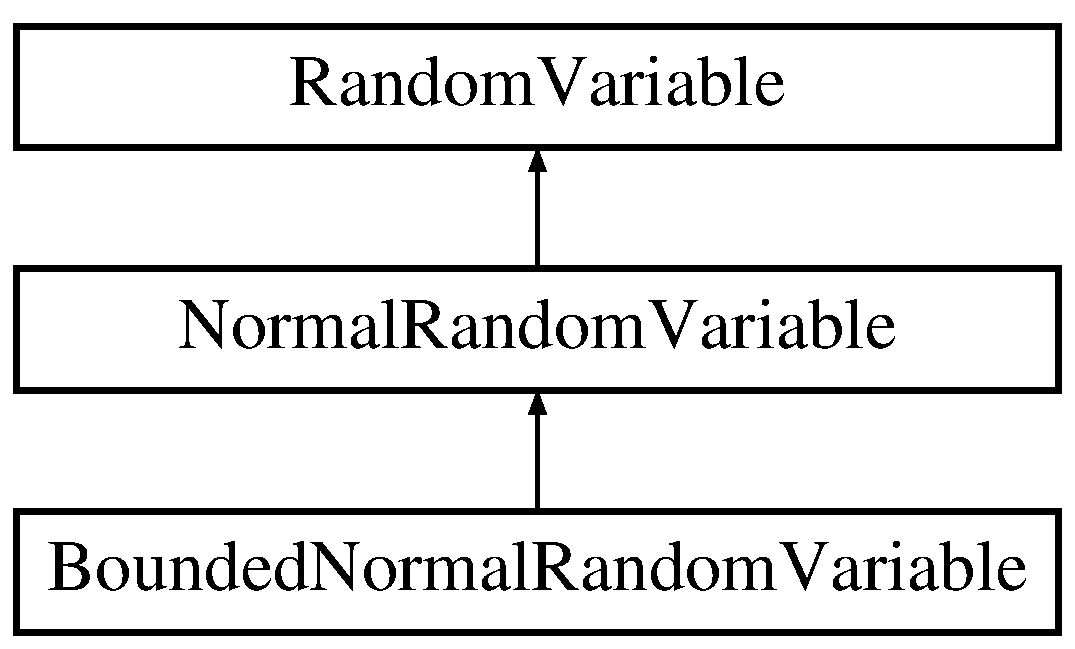
\includegraphics[height=3.000000cm]{classPecos_1_1BoundedNormalRandomVariable}
\end{center}
\end{figure}
\subsection*{Public Member Functions}
\begin{DoxyCompactItemize}
\item 
\hyperlink{classPecos_1_1BoundedNormalRandomVariable_a8d59131434909d023ca2821529c6c1fc}{Bounded\+Normal\+Random\+Variable} ()\label{classPecos_1_1BoundedNormalRandomVariable_a8d59131434909d023ca2821529c6c1fc}

\begin{DoxyCompactList}\small\item\em default constructor \end{DoxyCompactList}\item 
\hyperlink{classPecos_1_1BoundedNormalRandomVariable_a0e6c24b339d851e0d2fee9e94a0429bc}{Bounded\+Normal\+Random\+Variable} (Real \hyperlink{classPecos_1_1BoundedNormalRandomVariable_a962ffe5a3593be370d5c883365c060f4}{mean}, Real stdev, Real lwr, Real upr)\label{classPecos_1_1BoundedNormalRandomVariable_a0e6c24b339d851e0d2fee9e94a0429bc}

\begin{DoxyCompactList}\small\item\em alternate constructor \end{DoxyCompactList}\item 
\hyperlink{classPecos_1_1BoundedNormalRandomVariable_a7d09ec2c837d1853b97e0b40601ddf62}{$\sim$\+Bounded\+Normal\+Random\+Variable} ()\label{classPecos_1_1BoundedNormalRandomVariable_a7d09ec2c837d1853b97e0b40601ddf62}

\begin{DoxyCompactList}\small\item\em destructor \end{DoxyCompactList}\item 
Real \hyperlink{classPecos_1_1BoundedNormalRandomVariable_addd564e7f4f314e12d38df74d845f0d8}{cdf} (Real x) const \label{classPecos_1_1BoundedNormalRandomVariable_addd564e7f4f314e12d38df74d845f0d8}

\begin{DoxyCompactList}\small\item\em return the cumulative distribution function value of the random variable at x \end{DoxyCompactList}\item 
Real \hyperlink{classPecos_1_1BoundedNormalRandomVariable_a23c3b599e7e4788a9a5e9e93c3dbaf4d}{ccdf} (Real x) const \label{classPecos_1_1BoundedNormalRandomVariable_a23c3b599e7e4788a9a5e9e93c3dbaf4d}

\begin{DoxyCompactList}\small\item\em return the complementary cumulative distribution function value of the random variable at x \end{DoxyCompactList}\item 
Real \hyperlink{classPecos_1_1BoundedNormalRandomVariable_a918a1aac05ca349ea5313eebcba46c3e}{inverse\+\_\+cdf} (Real p\+\_\+cdf) const \label{classPecos_1_1BoundedNormalRandomVariable_a918a1aac05ca349ea5313eebcba46c3e}

\begin{DoxyCompactList}\small\item\em return the x value corresponding to a cumulative probability \end{DoxyCompactList}\item 
Real \hyperlink{classPecos_1_1BoundedNormalRandomVariable_afda003a1f59ff6930902cd5c8601f49b}{inverse\+\_\+ccdf} (Real p\+\_\+ccdf) const \label{classPecos_1_1BoundedNormalRandomVariable_afda003a1f59ff6930902cd5c8601f49b}

\begin{DoxyCompactList}\small\item\em return the x value corresponding to a complementary cumulative probability \end{DoxyCompactList}\item 
Real \hyperlink{classPecos_1_1BoundedNormalRandomVariable_a8ec69265f428e17c1707133cb137a819}{pdf} (Real x) const \label{classPecos_1_1BoundedNormalRandomVariable_a8ec69265f428e17c1707133cb137a819}

\begin{DoxyCompactList}\small\item\em return the value of the random variable\textquotesingle{}s probability density function at x \end{DoxyCompactList}\item 
Real \hyperlink{classPecos_1_1BoundedNormalRandomVariable_a6e2b6b6f13eedb2eb1ef3bc455a06392}{log\+\_\+pdf} (Real x) const \label{classPecos_1_1BoundedNormalRandomVariable_a6e2b6b6f13eedb2eb1ef3bc455a06392}

\begin{DoxyCompactList}\small\item\em return the value of the natural log of the random variable\textquotesingle{}s probability density function at x (useful for calculations of log density in Bayesian methods) \end{DoxyCompactList}\item 
Real \hyperlink{classPecos_1_1BoundedNormalRandomVariable_a5ccc16c04690f0c501f44c1ffae2bbd1}{log\+\_\+pdf\+\_\+gradient} (Real x) const \label{classPecos_1_1BoundedNormalRandomVariable_a5ccc16c04690f0c501f44c1ffae2bbd1}

\begin{DoxyCompactList}\small\item\em return the gradient of the natural log of the random variable\textquotesingle{}s probability density function at x (useful for defining M\+C\+MC proposal distributions in Bayesian methods) \end{DoxyCompactList}\item 
Real \hyperlink{classPecos_1_1BoundedNormalRandomVariable_a7b43f26f0f2bcdfef15d87e1f9399b33}{log\+\_\+pdf\+\_\+hessian} (Real x) const \label{classPecos_1_1BoundedNormalRandomVariable_a7b43f26f0f2bcdfef15d87e1f9399b33}

\begin{DoxyCompactList}\small\item\em return the Hessian of the natural log of the random variable\textquotesingle{}s probability density function at x (useful for defining M\+C\+MC proposal distributions in Bayesian methods) \end{DoxyCompactList}\item 
Real \hyperlink{classPecos_1_1BoundedNormalRandomVariable_aa891dab1ae9a225f493e3a0e5032b778}{parameter} (short dist\+\_\+param) const \label{classPecos_1_1BoundedNormalRandomVariable_aa891dab1ae9a225f493e3a0e5032b778}

\begin{DoxyCompactList}\small\item\em return the value of the named distribution parameter \end{DoxyCompactList}\item 
void \hyperlink{classPecos_1_1BoundedNormalRandomVariable_ae8e123224f588aee676d5d56d5ca900d}{parameter} (short dist\+\_\+param, Real val)\label{classPecos_1_1BoundedNormalRandomVariable_ae8e123224f588aee676d5d56d5ca900d}

\begin{DoxyCompactList}\small\item\em update the value of the named distribution parameter \end{DoxyCompactList}\item 
Real \hyperlink{classPecos_1_1BoundedNormalRandomVariable_a962ffe5a3593be370d5c883365c060f4}{mean} () const \label{classPecos_1_1BoundedNormalRandomVariable_a962ffe5a3593be370d5c883365c060f4}

\begin{DoxyCompactList}\small\item\em return the distribution mean \end{DoxyCompactList}\item 
Real \hyperlink{classPecos_1_1BoundedNormalRandomVariable_ae1fff19ce29a79d657043a598523635d}{median} () const \label{classPecos_1_1BoundedNormalRandomVariable_ae1fff19ce29a79d657043a598523635d}

\begin{DoxyCompactList}\small\item\em return the distribution mode \end{DoxyCompactList}\item 
Real \hyperlink{classPecos_1_1BoundedNormalRandomVariable_a72d3d6926edd929cb3f8e12baa655f70}{mode} () const \label{classPecos_1_1BoundedNormalRandomVariable_a72d3d6926edd929cb3f8e12baa655f70}

\begin{DoxyCompactList}\small\item\em return the distribution mode \end{DoxyCompactList}\item 
Real \hyperlink{classPecos_1_1BoundedNormalRandomVariable_a6a4ed9624d511f8a4e4f509c82cb0706}{standard\+\_\+deviation} () const \label{classPecos_1_1BoundedNormalRandomVariable_a6a4ed9624d511f8a4e4f509c82cb0706}

\begin{DoxyCompactList}\small\item\em return the distribution variance \end{DoxyCompactList}\item 
Real \hyperlink{classPecos_1_1BoundedNormalRandomVariable_a4b8b05b2a9af92dad9cc304c2925a4eb}{variance} () const \label{classPecos_1_1BoundedNormalRandomVariable_a4b8b05b2a9af92dad9cc304c2925a4eb}

\begin{DoxyCompactList}\small\item\em return the distribution variance \end{DoxyCompactList}\item 
Real\+Real\+Pair \hyperlink{classPecos_1_1BoundedNormalRandomVariable_a80e9024c98c6105a5eace8601a91b3d3}{moments} () const 
\begin{DoxyCompactList}\small\item\em return the distribution mean and standard deviation as a pair \end{DoxyCompactList}\item 
Real\+Real\+Pair \hyperlink{classPecos_1_1BoundedNormalRandomVariable_a4bdb95a8fa5fffaa0de5102f56963cf2}{bounds} () const \label{classPecos_1_1BoundedNormalRandomVariable_a4bdb95a8fa5fffaa0de5102f56963cf2}

\begin{DoxyCompactList}\small\item\em return the distribution lower and upper bounds as a pair \end{DoxyCompactList}\item 
Real \hyperlink{classPecos_1_1BoundedNormalRandomVariable_ae1cf1c07047d7ad9dbb899aa01138d54}{coefficient\+\_\+of\+\_\+variation} () const 
\begin{DoxyCompactList}\small\item\em compute the coefficient of variation (used to compute selected correlation warping factors); defined for semi-\/infinite distributions with nonzero mean (lognormal, exponential, gamma, frechet, weibull) \end{DoxyCompactList}\item 
Real \hyperlink{classPecos_1_1BoundedNormalRandomVariable_af889af8adfb262c9b74f573b2a9ffc99}{dx\+\_\+ds} (short dist\+\_\+param, short u\+\_\+type, Real x, Real z) const 
\item 
Real \hyperlink{classPecos_1_1BoundedNormalRandomVariable_af6b5fc528523180bed5fc3008dcea205}{dz\+\_\+ds\+\_\+factor} (short u\+\_\+type, Real x, Real z) const 
\item 
void {\bfseries update} (Real \hyperlink{classPecos_1_1BoundedNormalRandomVariable_a962ffe5a3593be370d5c883365c060f4}{mean}, Real stdev, Real lwr, Real upr)\label{classPecos_1_1BoundedNormalRandomVariable_add81a1f27687971ef4258150d5b35e92}

\end{DoxyCompactItemize}
\subsection*{Static Public Member Functions}
\begin{DoxyCompactItemize}
\item 
static Real {\bfseries pdf} (Real x, Real \hyperlink{classPecos_1_1BoundedNormalRandomVariable_a962ffe5a3593be370d5c883365c060f4}{mean}, Real std\+\_\+dev, Real lwr, Real upr)\label{classPecos_1_1BoundedNormalRandomVariable_ad9ad5dbcbf644f77992c234429589a83}

\item 
static Real {\bfseries cdf} (Real x, Real \hyperlink{classPecos_1_1BoundedNormalRandomVariable_a962ffe5a3593be370d5c883365c060f4}{mean}, Real std\+\_\+dev, Real lwr, Real upr)\label{classPecos_1_1BoundedNormalRandomVariable_aca0dd8dc49fd1def18904463bc0a97f7}

\end{DoxyCompactItemize}
\subsection*{Protected Attributes}
\begin{DoxyCompactItemize}
\item 
Real \hyperlink{classPecos_1_1BoundedNormalRandomVariable_a346dc528fe624cdf3ebb56fb9539f550}{lower\+Bnd}\label{classPecos_1_1BoundedNormalRandomVariable_a346dc528fe624cdf3ebb56fb9539f550}

\begin{DoxyCompactList}\small\item\em lower bound of bounded\+\_\+normal random variable \end{DoxyCompactList}\item 
Real \hyperlink{classPecos_1_1BoundedNormalRandomVariable_a671794a0fe385a29a595e98f44cde031}{upper\+Bnd}\label{classPecos_1_1BoundedNormalRandomVariable_a671794a0fe385a29a595e98f44cde031}

\begin{DoxyCompactList}\small\item\em upper bound of bounded\+\_\+normal random variable \end{DoxyCompactList}\end{DoxyCompactItemize}
\subsection*{Additional Inherited Members}


\subsection{Detailed Description}
Derived random variable class for bounded normal random variables. 

Manages lower and upper bounds. 

\subsection{Member Function Documentation}
\index{Pecos\+::\+Bounded\+Normal\+Random\+Variable@{Pecos\+::\+Bounded\+Normal\+Random\+Variable}!moments@{moments}}
\index{moments@{moments}!Pecos\+::\+Bounded\+Normal\+Random\+Variable@{Pecos\+::\+Bounded\+Normal\+Random\+Variable}}
\subsubsection[{\texorpdfstring{moments() const }{moments() const }}]{\setlength{\rightskip}{0pt plus 5cm}Real\+Real\+Pair moments (
\begin{DoxyParamCaption}
{}
\end{DoxyParamCaption}
) const\hspace{0.3cm}{\ttfamily [inline]}, {\ttfamily [virtual]}}\label{classPecos_1_1BoundedNormalRandomVariable_a80e9024c98c6105a5eace8601a91b3d3}


return the distribution mean and standard deviation as a pair 

default is only overridden when more efficient to compute together 

Reimplemented from \hyperlink{classPecos_1_1RandomVariable_a80e9024c98c6105a5eace8601a91b3d3}{Random\+Variable}.



References Normal\+Random\+Variable\+::gauss\+Mean, Normal\+Random\+Variable\+::gauss\+Std\+Dev, Bounded\+Normal\+Random\+Variable\+::lower\+Bnd, Normal\+Random\+Variable\+::std\+\_\+cdf(), Normal\+Random\+Variable\+::std\+\_\+pdf(), and Bounded\+Normal\+Random\+Variable\+::upper\+Bnd.



Referenced by Bounded\+Normal\+Random\+Variable\+::coefficient\+\_\+of\+\_\+variation().

\index{Pecos\+::\+Bounded\+Normal\+Random\+Variable@{Pecos\+::\+Bounded\+Normal\+Random\+Variable}!coefficient\+\_\+of\+\_\+variation@{coefficient\+\_\+of\+\_\+variation}}
\index{coefficient\+\_\+of\+\_\+variation@{coefficient\+\_\+of\+\_\+variation}!Pecos\+::\+Bounded\+Normal\+Random\+Variable@{Pecos\+::\+Bounded\+Normal\+Random\+Variable}}
\subsubsection[{\texorpdfstring{coefficient\+\_\+of\+\_\+variation() const }{coefficient_of_variation() const }}]{\setlength{\rightskip}{0pt plus 5cm}Real coefficient\+\_\+of\+\_\+variation (
\begin{DoxyParamCaption}
{}
\end{DoxyParamCaption}
) const\hspace{0.3cm}{\ttfamily [inline]}, {\ttfamily [virtual]}}\label{classPecos_1_1BoundedNormalRandomVariable_ae1cf1c07047d7ad9dbb899aa01138d54}


compute the coefficient of variation (used to compute selected correlation warping factors); defined for semi-\/infinite distributions with nonzero mean (lognormal, exponential, gamma, frechet, weibull) 

default is only overridden when more efficient to compute together 

Reimplemented from \hyperlink{classPecos_1_1RandomVariable_ae1cf1c07047d7ad9dbb899aa01138d54}{Random\+Variable}.



References Bounded\+Normal\+Random\+Variable\+::dx\+\_\+ds(), and Bounded\+Normal\+Random\+Variable\+::moments().

\index{Pecos\+::\+Bounded\+Normal\+Random\+Variable@{Pecos\+::\+Bounded\+Normal\+Random\+Variable}!dx\+\_\+ds@{dx\+\_\+ds}}
\index{dx\+\_\+ds@{dx\+\_\+ds}!Pecos\+::\+Bounded\+Normal\+Random\+Variable@{Pecos\+::\+Bounded\+Normal\+Random\+Variable}}
\subsubsection[{\texorpdfstring{dx\+\_\+ds(short dist\+\_\+param, short u\+\_\+type, Real x, Real z) const }{dx_ds(short dist_param, short u_type, Real x, Real z) const }}]{\setlength{\rightskip}{0pt plus 5cm}Real dx\+\_\+ds (
\begin{DoxyParamCaption}
\item[{short}]{dist\+\_\+param, }
\item[{short}]{u\+\_\+type, }
\item[{Real}]{x, }
\item[{Real}]{z}
\end{DoxyParamCaption}
) const\hspace{0.3cm}{\ttfamily [inline]}, {\ttfamily [virtual]}}\label{classPecos_1_1BoundedNormalRandomVariable_af889af8adfb262c9b74f573b2a9ffc99}
dx/ds is derived by differentiating \hyperlink{classPecos_1_1NatafTransformation_a5feeecf846fc017c5a28eccb4e955dc1}{Nataf\+Transformation\+::trans\+\_\+\+Z\+\_\+to\+\_\+\+X()} with respect to distribution parameter s. dz/ds is zero if uncorrelated, while \hyperlink{classPecos_1_1BoundedNormalRandomVariable_af6b5fc528523180bed5fc3008dcea205}{dz\+\_\+ds\+\_\+factor()} manages contributions in the correlated case. 

Reimplemented from \hyperlink{classPecos_1_1RandomVariable_af889af8adfb262c9b74f573b2a9ffc99}{Random\+Variable}.



References Bounded\+Normal\+Random\+Variable\+::dz\+\_\+ds\+\_\+factor(), Normal\+Random\+Variable\+::gauss\+Mean, Normal\+Random\+Variable\+::gauss\+Std\+Dev, Bounded\+Normal\+Random\+Variable\+::lower\+Bnd, Normal\+Random\+Variable\+::std\+\_\+cdf(), Normal\+Random\+Variable\+::std\+\_\+pdf(), and Bounded\+Normal\+Random\+Variable\+::upper\+Bnd.



Referenced by Bounded\+Normal\+Random\+Variable\+::coefficient\+\_\+of\+\_\+variation().

\index{Pecos\+::\+Bounded\+Normal\+Random\+Variable@{Pecos\+::\+Bounded\+Normal\+Random\+Variable}!dz\+\_\+ds\+\_\+factor@{dz\+\_\+ds\+\_\+factor}}
\index{dz\+\_\+ds\+\_\+factor@{dz\+\_\+ds\+\_\+factor}!Pecos\+::\+Bounded\+Normal\+Random\+Variable@{Pecos\+::\+Bounded\+Normal\+Random\+Variable}}
\subsubsection[{\texorpdfstring{dz\+\_\+ds\+\_\+factor(short u\+\_\+type, Real x, Real z) const }{dz_ds_factor(short u_type, Real x, Real z) const }}]{\setlength{\rightskip}{0pt plus 5cm}Real dz\+\_\+ds\+\_\+factor (
\begin{DoxyParamCaption}
\item[{short}]{u\+\_\+type, }
\item[{Real}]{x, }
\item[{Real}]{z}
\end{DoxyParamCaption}
) const\hspace{0.3cm}{\ttfamily [inline]}, {\ttfamily [virtual]}}\label{classPecos_1_1BoundedNormalRandomVariable_af6b5fc528523180bed5fc3008dcea205}
dx/ds is derived by differentiating \hyperlink{classPecos_1_1NatafTransformation_a5feeecf846fc017c5a28eccb4e955dc1}{Nataf\+Transformation\+::trans\+\_\+\+Z\+\_\+to\+\_\+\+X()} with respect to distribution parameter s. For the uncorrelated case, u and z are constants. For the correlated case, u is a constant, but z(s) = L(s) u due to Nataf dependence on s and dz/ds = d\+L/ds u. 

Reimplemented from \hyperlink{classPecos_1_1RandomVariable_af6b5fc528523180bed5fc3008dcea205}{Random\+Variable}.



References Normal\+Random\+Variable\+::gauss\+Mean, Normal\+Random\+Variable\+::gauss\+Std\+Dev, Bounded\+Normal\+Random\+Variable\+::lower\+Bnd, Bounded\+Normal\+Random\+Variable\+::mean(), Normal\+Random\+Variable\+::std\+\_\+cdf(), Normal\+Random\+Variable\+::std\+\_\+pdf(), and Bounded\+Normal\+Random\+Variable\+::upper\+Bnd.



Referenced by Bounded\+Normal\+Random\+Variable\+::dx\+\_\+ds().



The documentation for this class was generated from the following file\+:\begin{DoxyCompactItemize}
\item 
Bounded\+Normal\+Random\+Variable.\+hpp\end{DoxyCompactItemize}

\section{Charlier\+Orthog\+Polynomial Class Reference}
\label{classPecos_1_1CharlierOrthogPolynomial}\index{Charlier\+Orthog\+Polynomial@{Charlier\+Orthog\+Polynomial}}


One-\/dimensional Charlier polynomial.  


Inheritance diagram for Charlier\+Orthog\+Polynomial\+:\begin{figure}[H]
\begin{center}
\leavevmode
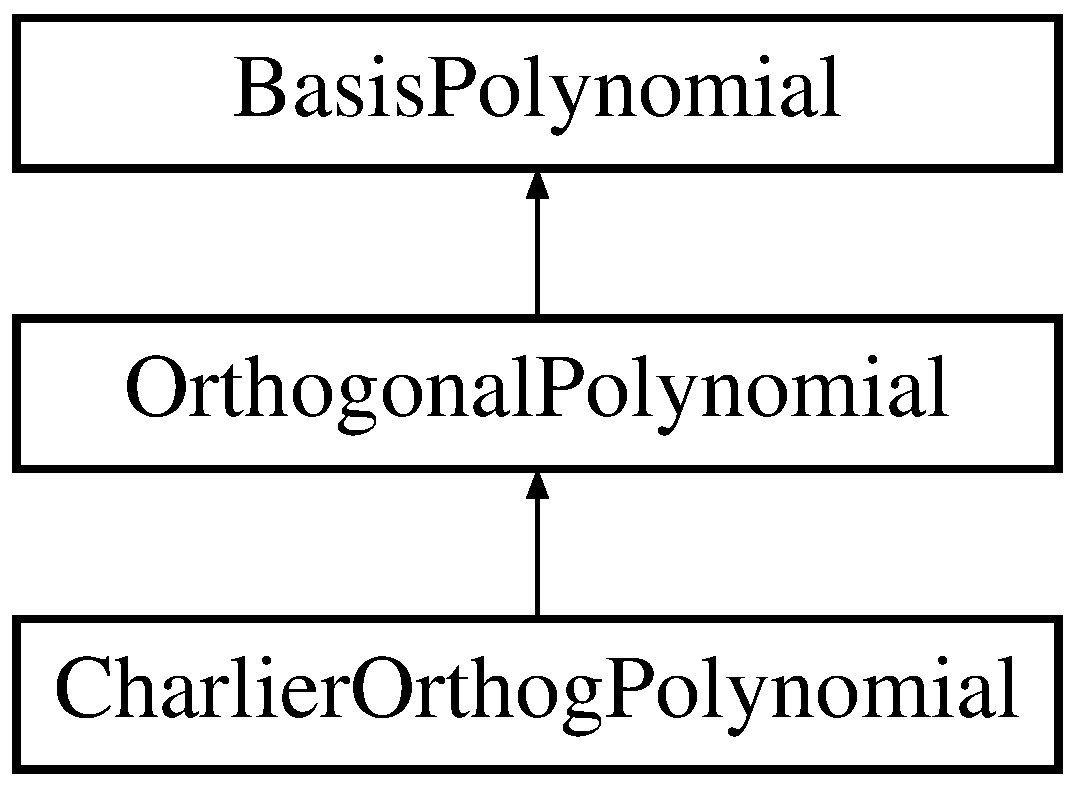
\includegraphics[height=3.000000cm]{classPecos_1_1CharlierOrthogPolynomial}
\end{center}
\end{figure}
\subsection*{Public Member Functions}
\begin{DoxyCompactItemize}
\item 
\hyperlink{classPecos_1_1CharlierOrthogPolynomial_a2fbeb789bb30be5edeeb764b942f9b2a}{Charlier\+Orthog\+Polynomial} ()\label{classPecos_1_1CharlierOrthogPolynomial_a2fbeb789bb30be5edeeb764b942f9b2a}

\begin{DoxyCompactList}\small\item\em default constructor \end{DoxyCompactList}\item 
\hyperlink{classPecos_1_1CharlierOrthogPolynomial_a8867cc03efde2b2a285f5b133a5c1b37}{$\sim$\+Charlier\+Orthog\+Polynomial} ()\label{classPecos_1_1CharlierOrthogPolynomial_a8867cc03efde2b2a285f5b133a5c1b37}

\begin{DoxyCompactList}\small\item\em destructor \end{DoxyCompactList}\end{DoxyCompactItemize}
\subsection*{Protected Member Functions}
\begin{DoxyCompactItemize}
\item 
Real \hyperlink{classPecos_1_1CharlierOrthogPolynomial_a8792a858ac05a2158880e876f9da2019}{type1\+\_\+value} (Real x, unsigned short order)
\begin{DoxyCompactList}\small\item\em retrieve the value of the n\+\_\+th type 1 polynomial for a given parameter x using traditional characteristic polynomial formulation \end{DoxyCompactList}\item 
Real \hyperlink{classPecos_1_1CharlierOrthogPolynomial_aac6751aa35bf5fcb42c520a322fc26dc}{type1\+\_\+gradient} (Real x, unsigned short order)
\begin{DoxyCompactList}\small\item\em retrieve the gradient of the n\+\_\+th type 1 polynomial for a given parameter x using traditional characteristic polynomial formulation \end{DoxyCompactList}\item 
Real \hyperlink{classPecos_1_1CharlierOrthogPolynomial_ae957c8c2e7ea13728bafbad0c9b2996e}{type1\+\_\+hessian} (Real x, unsigned short order)
\begin{DoxyCompactList}\small\item\em retrieve the Hessian of the n\+\_\+th type 1 polynomial for a given parameter x using traditional characteristic polynomial formulation \end{DoxyCompactList}\item 
Real \hyperlink{classPecos_1_1CharlierOrthogPolynomial_a77c0dbb874af1190d448d01da6efbe4e}{norm\+\_\+squared} (unsigned short order)
\begin{DoxyCompactList}\small\item\em returns the norm-\/squared of the n\+\_\+th order polynomial defined by the inner product $<$Poly\+\_\+n, Poly\+\_\+n$>$ = $\vert$$\vert$\+Poly\+\_\+n$\vert$$\vert$$^\wedge$2 \end{DoxyCompactList}\item 
Real \hyperlink{classPecos_1_1CharlierOrthogPolynomial_a997bdeddf670667c476513fcacc779ca}{alpha\+\_\+polynomial} () const \label{classPecos_1_1CharlierOrthogPolynomial_a997bdeddf670667c476513fcacc779ca}

\begin{DoxyCompactList}\small\item\em return alpha\+Poly \end{DoxyCompactList}\item 
void \hyperlink{classPecos_1_1CharlierOrthogPolynomial_aeeb4ce11a8d413209be1ec08eced8728}{alpha\+\_\+stat} (Real alpha)\label{classPecos_1_1CharlierOrthogPolynomial_aeeb4ce11a8d413209be1ec08eced8728}

\begin{DoxyCompactList}\small\item\em set beta\+Poly \end{DoxyCompactList}\end{DoxyCompactItemize}
\subsection*{Private Attributes}
\begin{DoxyCompactItemize}
\item 
Real \hyperlink{classPecos_1_1CharlierOrthogPolynomial_a11666846719189915a02ac6f1f96e393}{alpha\+Poly}\label{classPecos_1_1CharlierOrthogPolynomial_a11666846719189915a02ac6f1f96e393}

\begin{DoxyCompactList}\small\item\em Poisson distributioon is the probability that a realziations of a random variable X with mean alpha\+\_\+stat occurring k times in a fixed interval. expected value of the random variable X. \end{DoxyCompactList}\end{DoxyCompactItemize}
\subsection*{Additional Inherited Members}


\subsection{Detailed Description}
One-\/dimensional Charlier polynomial. 

\subsection{Member Function Documentation}
\index{Pecos\+::\+Charlier\+Orthog\+Polynomial@{Pecos\+::\+Charlier\+Orthog\+Polynomial}!type1\+\_\+value@{type1\+\_\+value}}
\index{type1\+\_\+value@{type1\+\_\+value}!Pecos\+::\+Charlier\+Orthog\+Polynomial@{Pecos\+::\+Charlier\+Orthog\+Polynomial}}
\subsubsection[{\texorpdfstring{type1\+\_\+value(\+Real x, unsigned short order)}{type1_value(Real x, unsigned short order)}}]{\setlength{\rightskip}{0pt plus 5cm}Real type1\+\_\+value (
\begin{DoxyParamCaption}
\item[{Real}]{x, }
\item[{unsigned short}]{n}
\end{DoxyParamCaption}
)\hspace{0.3cm}{\ttfamily [protected]}, {\ttfamily [virtual]}}\label{classPecos_1_1CharlierOrthogPolynomial_a8792a858ac05a2158880e876f9da2019}


retrieve the value of the n\+\_\+th type 1 polynomial for a given parameter x using traditional characteristic polynomial formulation 

For orthogonal polynomials, n specifies the order of the polynomial, whereas for interpolation polynomials, it identifies the interpolant for the n-\/th point. 

Reimplemented from \hyperlink{classPecos_1_1BasisPolynomial_a1fab871e99cec3a1933a2b1e9ed8a625}{Basis\+Polynomial}.



References Charlier\+Orthog\+Polynomial\+::alpha\+Poly.



Referenced by Charlier\+Orthog\+Polynomial\+::type1\+\_\+gradient().

\index{Pecos\+::\+Charlier\+Orthog\+Polynomial@{Pecos\+::\+Charlier\+Orthog\+Polynomial}!type1\+\_\+gradient@{type1\+\_\+gradient}}
\index{type1\+\_\+gradient@{type1\+\_\+gradient}!Pecos\+::\+Charlier\+Orthog\+Polynomial@{Pecos\+::\+Charlier\+Orthog\+Polynomial}}
\subsubsection[{\texorpdfstring{type1\+\_\+gradient(\+Real x, unsigned short order)}{type1_gradient(Real x, unsigned short order)}}]{\setlength{\rightskip}{0pt plus 5cm}Real type1\+\_\+gradient (
\begin{DoxyParamCaption}
\item[{Real}]{x, }
\item[{unsigned short}]{n}
\end{DoxyParamCaption}
)\hspace{0.3cm}{\ttfamily [protected]}, {\ttfamily [virtual]}}\label{classPecos_1_1CharlierOrthogPolynomial_aac6751aa35bf5fcb42c520a322fc26dc}


retrieve the gradient of the n\+\_\+th type 1 polynomial for a given parameter x using traditional characteristic polynomial formulation 

For orthogonal polynomials, n specifies the order of the polynomial, whereas for interpolation polynomials, it identifies the interpolant for the n-\/th point. 

Reimplemented from \hyperlink{classPecos_1_1BasisPolynomial_a6f69ec84983f551e7e0e4a18b78b4498}{Basis\+Polynomial}.



References Charlier\+Orthog\+Polynomial\+::alpha\+Poly, and Charlier\+Orthog\+Polynomial\+::type1\+\_\+value().



Referenced by Charlier\+Orthog\+Polynomial\+::type1\+\_\+hessian().

\index{Pecos\+::\+Charlier\+Orthog\+Polynomial@{Pecos\+::\+Charlier\+Orthog\+Polynomial}!type1\+\_\+hessian@{type1\+\_\+hessian}}
\index{type1\+\_\+hessian@{type1\+\_\+hessian}!Pecos\+::\+Charlier\+Orthog\+Polynomial@{Pecos\+::\+Charlier\+Orthog\+Polynomial}}
\subsubsection[{\texorpdfstring{type1\+\_\+hessian(\+Real x, unsigned short order)}{type1_hessian(Real x, unsigned short order)}}]{\setlength{\rightskip}{0pt plus 5cm}Real type1\+\_\+hessian (
\begin{DoxyParamCaption}
\item[{Real}]{x, }
\item[{unsigned short}]{n}
\end{DoxyParamCaption}
)\hspace{0.3cm}{\ttfamily [protected]}, {\ttfamily [virtual]}}\label{classPecos_1_1CharlierOrthogPolynomial_ae957c8c2e7ea13728bafbad0c9b2996e}


retrieve the Hessian of the n\+\_\+th type 1 polynomial for a given parameter x using traditional characteristic polynomial formulation 

For orthogonal polynomials, n specifies the order of the polynomial, whereas for interpolation polynomials, it identifies the interpolant for the n-\/th point. 

Reimplemented from \hyperlink{classPecos_1_1BasisPolynomial_a07d617dad8572dd606371e6c89ab6c35}{Basis\+Polynomial}.



References Charlier\+Orthog\+Polynomial\+::alpha\+Poly, and Charlier\+Orthog\+Polynomial\+::type1\+\_\+gradient().

\index{Pecos\+::\+Charlier\+Orthog\+Polynomial@{Pecos\+::\+Charlier\+Orthog\+Polynomial}!norm\+\_\+squared@{norm\+\_\+squared}}
\index{norm\+\_\+squared@{norm\+\_\+squared}!Pecos\+::\+Charlier\+Orthog\+Polynomial@{Pecos\+::\+Charlier\+Orthog\+Polynomial}}
\subsubsection[{\texorpdfstring{norm\+\_\+squared(unsigned short order)}{norm_squared(unsigned short order)}}]{\setlength{\rightskip}{0pt plus 5cm}Real norm\+\_\+squared (
\begin{DoxyParamCaption}
\item[{unsigned short}]{n}
\end{DoxyParamCaption}
)\hspace{0.3cm}{\ttfamily [protected]}, {\ttfamily [virtual]}}\label{classPecos_1_1CharlierOrthogPolynomial_a77c0dbb874af1190d448d01da6efbe4e}


returns the norm-\/squared of the n\+\_\+th order polynomial defined by the inner product $<$Poly\+\_\+n, Poly\+\_\+n$>$ = $\vert$$\vert$\+Poly\+\_\+n$\vert$$\vert$$^\wedge$2 

This is defined only for orthogonal polynomials. 

Reimplemented from \hyperlink{classPecos_1_1BasisPolynomial_ab74383be309d74823f2e5e85dad739b2}{Basis\+Polynomial}.



References Charlier\+Orthog\+Polynomial\+::alpha\+Poly.



The documentation for this class was generated from the following files\+:\begin{DoxyCompactItemize}
\item 
Charlier\+Orthog\+Polynomial.\+hpp\item 
Charlier\+Orthog\+Polynomial.\+cpp\end{DoxyCompactItemize}

\section{Chebyshev\+Orthog\+Polynomial Class Reference}
\label{classPecos_1_1ChebyshevOrthogPolynomial}\index{Chebyshev\+Orthog\+Polynomial@{Chebyshev\+Orthog\+Polynomial}}


Derived orthogonal polynomial class for Chebyshev polynomials.  


Inheritance diagram for Chebyshev\+Orthog\+Polynomial\+:\begin{figure}[H]
\begin{center}
\leavevmode
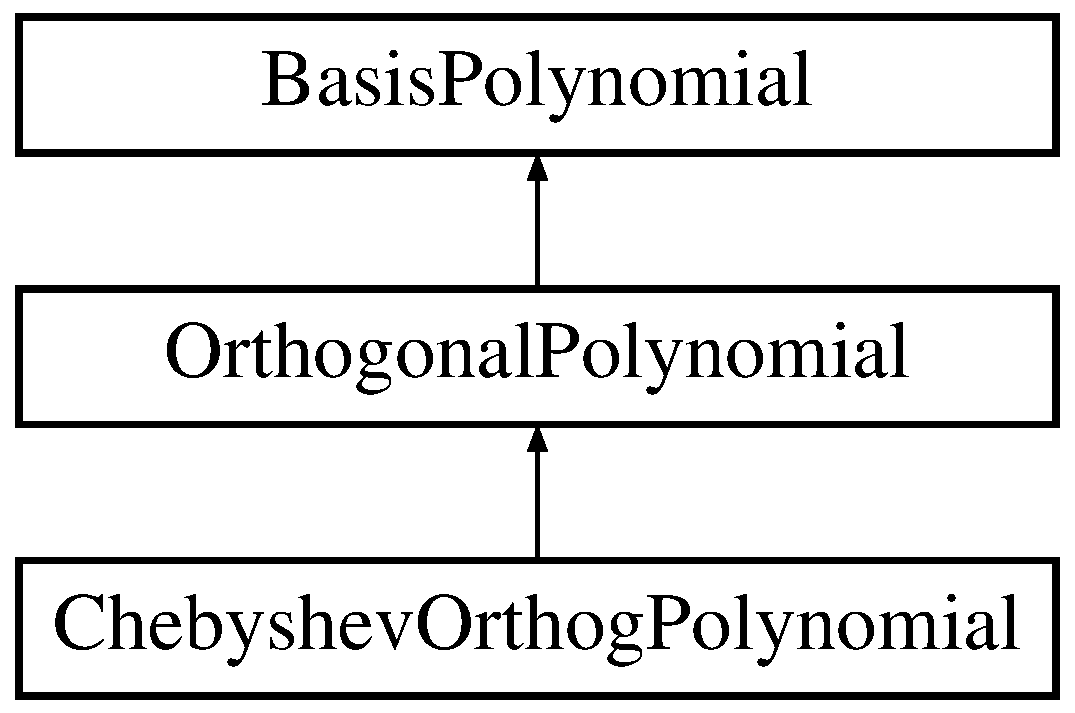
\includegraphics[height=3.000000cm]{classPecos_1_1ChebyshevOrthogPolynomial}
\end{center}
\end{figure}
\subsection*{Public Member Functions}
\begin{DoxyCompactItemize}
\item 
\hyperlink{classPecos_1_1ChebyshevOrthogPolynomial_ac40cce2bd16396062e4f40c84a275733}{Chebyshev\+Orthog\+Polynomial} (short colloc\+\_\+rule)\label{classPecos_1_1ChebyshevOrthogPolynomial_ac40cce2bd16396062e4f40c84a275733}

\begin{DoxyCompactList}\small\item\em extended constructor \end{DoxyCompactList}\item 
\hyperlink{classPecos_1_1ChebyshevOrthogPolynomial_a76aaaf7a64cb6711fb3a06d1624459a6}{Chebyshev\+Orthog\+Polynomial} ()\label{classPecos_1_1ChebyshevOrthogPolynomial_a76aaaf7a64cb6711fb3a06d1624459a6}

\begin{DoxyCompactList}\small\item\em default constructor \end{DoxyCompactList}\item 
\hyperlink{classPecos_1_1ChebyshevOrthogPolynomial_aad18404cb3d8b997796220d180da0e6c}{$\sim$\+Chebyshev\+Orthog\+Polynomial} ()\label{classPecos_1_1ChebyshevOrthogPolynomial_aad18404cb3d8b997796220d180da0e6c}

\begin{DoxyCompactList}\small\item\em destructor \end{DoxyCompactList}\end{DoxyCompactItemize}
\subsection*{Protected Member Functions}
\begin{DoxyCompactItemize}
\item 
Real \hyperlink{classPecos_1_1ChebyshevOrthogPolynomial_a8792a858ac05a2158880e876f9da2019}{type1\+\_\+value} (Real x, unsigned short order)
\begin{DoxyCompactList}\small\item\em retrieve the value of the n\+\_\+th type 1 polynomial for a given parameter x using traditional characteristic polynomial formulation \end{DoxyCompactList}\item 
Real \hyperlink{classPecos_1_1ChebyshevOrthogPolynomial_aac6751aa35bf5fcb42c520a322fc26dc}{type1\+\_\+gradient} (Real x, unsigned short order)
\begin{DoxyCompactList}\small\item\em retrieve the gradient of the n\+\_\+th type 1 polynomial for a given parameter x using traditional characteristic polynomial formulation \end{DoxyCompactList}\item 
Real \hyperlink{classPecos_1_1ChebyshevOrthogPolynomial_ae957c8c2e7ea13728bafbad0c9b2996e}{type1\+\_\+hessian} (Real x, unsigned short order)
\begin{DoxyCompactList}\small\item\em retrieve the Hessian of the n\+\_\+th type 1 polynomial for a given parameter x using traditional characteristic polynomial formulation \end{DoxyCompactList}\item 
Real \hyperlink{classPecos_1_1ChebyshevOrthogPolynomial_a77c0dbb874af1190d448d01da6efbe4e}{norm\+\_\+squared} (unsigned short order)
\begin{DoxyCompactList}\small\item\em returns the norm-\/squared of the n\+\_\+th order polynomial defined by the inner product $<$Poly\+\_\+n, Poly\+\_\+n$>$ = $\vert$$\vert$\+Poly\+\_\+n$\vert$$\vert$$^\wedge$2 \end{DoxyCompactList}\item 
const Real\+Array \& \hyperlink{classPecos_1_1ChebyshevOrthogPolynomial_a10873b28f1284aff4ea214e00c4f86dd}{collocation\+\_\+points} (unsigned short order)
\begin{DoxyCompactList}\small\item\em return collocation points corresponding to orthogonal polynomial order n \end{DoxyCompactList}\item 
const Real\+Array \& \hyperlink{classPecos_1_1ChebyshevOrthogPolynomial_aa010321cf47465dca5725fa15ba58bf6}{type1\+\_\+collocation\+\_\+weights} (unsigned short order)
\begin{DoxyCompactList}\small\item\em return the type 1 collocation weights corresponding to a point set of size order \end{DoxyCompactList}\item 
Real \hyperlink{classPecos_1_1ChebyshevOrthogPolynomial_a8c1e8d014e82efc5a1c20f973b5bc715}{length\+\_\+scale} () const 
\end{DoxyCompactItemize}
\subsection*{Additional Inherited Members}


\subsection{Detailed Description}
Derived orthogonal polynomial class for Chebyshev polynomials. 

The \hyperlink{classPecos_1_1ChebyshevOrthogPolynomial}{Chebyshev\+Orthog\+Polynomial} class evaluates a univariate Chebyshev polynomial of the first kind (T\+\_\+n(x)) of a particular order. These polynomials are orthogonal with respect to the weight function 1/sqrt(1-\/x$^\wedge$2) when integrated over the support range of \mbox{[}-\/1,+1\mbox{]}. It enables (mixed) multidimensional orthogonal polynomial basis functions within \hyperlink{classPecos_1_1OrthogPolyApproximation}{Orthog\+Poly\+Approximation}. Chebyshev polynomials are a special case of the more general Jacobi polynomials (implemented separately). 

\subsection{Member Function Documentation}
\index{Pecos\+::\+Chebyshev\+Orthog\+Polynomial@{Pecos\+::\+Chebyshev\+Orthog\+Polynomial}!type1\+\_\+value@{type1\+\_\+value}}
\index{type1\+\_\+value@{type1\+\_\+value}!Pecos\+::\+Chebyshev\+Orthog\+Polynomial@{Pecos\+::\+Chebyshev\+Orthog\+Polynomial}}
\subsubsection[{\texorpdfstring{type1\+\_\+value(\+Real x, unsigned short order)}{type1_value(Real x, unsigned short order)}}]{\setlength{\rightskip}{0pt plus 5cm}Real type1\+\_\+value (
\begin{DoxyParamCaption}
\item[{Real}]{x, }
\item[{unsigned short}]{n}
\end{DoxyParamCaption}
)\hspace{0.3cm}{\ttfamily [protected]}, {\ttfamily [virtual]}}\label{classPecos_1_1ChebyshevOrthogPolynomial_a8792a858ac05a2158880e876f9da2019}


retrieve the value of the n\+\_\+th type 1 polynomial for a given parameter x using traditional characteristic polynomial formulation 

For orthogonal polynomials, n specifies the order of the polynomial, whereas for interpolation polynomials, it identifies the interpolant for the n-\/th point. 

Reimplemented from \hyperlink{classPecos_1_1BasisPolynomial_a1fab871e99cec3a1933a2b1e9ed8a625}{Basis\+Polynomial}.



Referenced by Chebyshev\+Orthog\+Polynomial\+::type1\+\_\+gradient().

\index{Pecos\+::\+Chebyshev\+Orthog\+Polynomial@{Pecos\+::\+Chebyshev\+Orthog\+Polynomial}!type1\+\_\+gradient@{type1\+\_\+gradient}}
\index{type1\+\_\+gradient@{type1\+\_\+gradient}!Pecos\+::\+Chebyshev\+Orthog\+Polynomial@{Pecos\+::\+Chebyshev\+Orthog\+Polynomial}}
\subsubsection[{\texorpdfstring{type1\+\_\+gradient(\+Real x, unsigned short order)}{type1_gradient(Real x, unsigned short order)}}]{\setlength{\rightskip}{0pt plus 5cm}Real type1\+\_\+gradient (
\begin{DoxyParamCaption}
\item[{Real}]{x, }
\item[{unsigned short}]{n}
\end{DoxyParamCaption}
)\hspace{0.3cm}{\ttfamily [protected]}, {\ttfamily [virtual]}}\label{classPecos_1_1ChebyshevOrthogPolynomial_aac6751aa35bf5fcb42c520a322fc26dc}


retrieve the gradient of the n\+\_\+th type 1 polynomial for a given parameter x using traditional characteristic polynomial formulation 

For orthogonal polynomials, n specifies the order of the polynomial, whereas for interpolation polynomials, it identifies the interpolant for the n-\/th point. 

Reimplemented from \hyperlink{classPecos_1_1BasisPolynomial_a6f69ec84983f551e7e0e4a18b78b4498}{Basis\+Polynomial}.



References Chebyshev\+Orthog\+Polynomial\+::type1\+\_\+value().



Referenced by Chebyshev\+Orthog\+Polynomial\+::type1\+\_\+hessian().

\index{Pecos\+::\+Chebyshev\+Orthog\+Polynomial@{Pecos\+::\+Chebyshev\+Orthog\+Polynomial}!type1\+\_\+hessian@{type1\+\_\+hessian}}
\index{type1\+\_\+hessian@{type1\+\_\+hessian}!Pecos\+::\+Chebyshev\+Orthog\+Polynomial@{Pecos\+::\+Chebyshev\+Orthog\+Polynomial}}
\subsubsection[{\texorpdfstring{type1\+\_\+hessian(\+Real x, unsigned short order)}{type1_hessian(Real x, unsigned short order)}}]{\setlength{\rightskip}{0pt plus 5cm}Real type1\+\_\+hessian (
\begin{DoxyParamCaption}
\item[{Real}]{x, }
\item[{unsigned short}]{n}
\end{DoxyParamCaption}
)\hspace{0.3cm}{\ttfamily [protected]}, {\ttfamily [virtual]}}\label{classPecos_1_1ChebyshevOrthogPolynomial_ae957c8c2e7ea13728bafbad0c9b2996e}


retrieve the Hessian of the n\+\_\+th type 1 polynomial for a given parameter x using traditional characteristic polynomial formulation 

For orthogonal polynomials, n specifies the order of the polynomial, whereas for interpolation polynomials, it identifies the interpolant for the n-\/th point. 

Reimplemented from \hyperlink{classPecos_1_1BasisPolynomial_a07d617dad8572dd606371e6c89ab6c35}{Basis\+Polynomial}.



References Chebyshev\+Orthog\+Polynomial\+::type1\+\_\+gradient().

\index{Pecos\+::\+Chebyshev\+Orthog\+Polynomial@{Pecos\+::\+Chebyshev\+Orthog\+Polynomial}!norm\+\_\+squared@{norm\+\_\+squared}}
\index{norm\+\_\+squared@{norm\+\_\+squared}!Pecos\+::\+Chebyshev\+Orthog\+Polynomial@{Pecos\+::\+Chebyshev\+Orthog\+Polynomial}}
\subsubsection[{\texorpdfstring{norm\+\_\+squared(unsigned short order)}{norm_squared(unsigned short order)}}]{\setlength{\rightskip}{0pt plus 5cm}Real norm\+\_\+squared (
\begin{DoxyParamCaption}
\item[{unsigned short}]{n}
\end{DoxyParamCaption}
)\hspace{0.3cm}{\ttfamily [protected]}, {\ttfamily [virtual]}}\label{classPecos_1_1ChebyshevOrthogPolynomial_a77c0dbb874af1190d448d01da6efbe4e}


returns the norm-\/squared of the n\+\_\+th order polynomial defined by the inner product $<$Poly\+\_\+n, Poly\+\_\+n$>$ = $\vert$$\vert$\+Poly\+\_\+n$\vert$$\vert$$^\wedge$2 

This is defined only for orthogonal polynomials. 

Reimplemented from \hyperlink{classPecos_1_1BasisPolynomial_ab74383be309d74823f2e5e85dad739b2}{Basis\+Polynomial}.



References Chebyshev\+Orthog\+Polynomial\+::collocation\+\_\+points().

\index{Pecos\+::\+Chebyshev\+Orthog\+Polynomial@{Pecos\+::\+Chebyshev\+Orthog\+Polynomial}!collocation\+\_\+points@{collocation\+\_\+points}}
\index{collocation\+\_\+points@{collocation\+\_\+points}!Pecos\+::\+Chebyshev\+Orthog\+Polynomial@{Pecos\+::\+Chebyshev\+Orthog\+Polynomial}}
\subsubsection[{\texorpdfstring{collocation\+\_\+points(unsigned short order)}{collocation_points(unsigned short order)}}]{\setlength{\rightskip}{0pt plus 5cm}const Real\+Array \& collocation\+\_\+points (
\begin{DoxyParamCaption}
\item[{unsigned short}]{n}
\end{DoxyParamCaption}
)\hspace{0.3cm}{\ttfamily [protected]}, {\ttfamily [virtual]}}\label{classPecos_1_1ChebyshevOrthogPolynomial_a10873b28f1284aff4ea214e00c4f86dd}


return collocation points corresponding to orthogonal polynomial order n 

This is defined for orthogonal and piecewise interpolation polynomials. 

Reimplemented from \hyperlink{classPecos_1_1BasisPolynomial_a0f96bd4e27ddc5c44117e7b68744b5a4}{Basis\+Polynomial}.



References Orthogonal\+Polynomial\+::colloc\+Points, Orthogonal\+Polynomial\+::colloc\+Rule, and Chebyshev\+Orthog\+Polynomial\+::type1\+\_\+collocation\+\_\+weights().



Referenced by Chebyshev\+Orthog\+Polynomial\+::norm\+\_\+squared().

\index{Pecos\+::\+Chebyshev\+Orthog\+Polynomial@{Pecos\+::\+Chebyshev\+Orthog\+Polynomial}!type1\+\_\+collocation\+\_\+weights@{type1\+\_\+collocation\+\_\+weights}}
\index{type1\+\_\+collocation\+\_\+weights@{type1\+\_\+collocation\+\_\+weights}!Pecos\+::\+Chebyshev\+Orthog\+Polynomial@{Pecos\+::\+Chebyshev\+Orthog\+Polynomial}}
\subsubsection[{\texorpdfstring{type1\+\_\+collocation\+\_\+weights(unsigned short order)}{type1_collocation_weights(unsigned short order)}}]{\setlength{\rightskip}{0pt plus 5cm}const Real\+Array \& type1\+\_\+collocation\+\_\+weights (
\begin{DoxyParamCaption}
\item[{unsigned short}]{order}
\end{DoxyParamCaption}
)\hspace{0.3cm}{\ttfamily [protected]}, {\ttfamily [virtual]}}\label{classPecos_1_1ChebyshevOrthogPolynomial_aa010321cf47465dca5725fa15ba58bf6}


return the type 1 collocation weights corresponding to a point set of size order 

This is defined for orthogonal and piecewise interpolation polynomials. 

Reimplemented from \hyperlink{classPecos_1_1BasisPolynomial_aa010321cf47465dca5725fa15ba58bf6}{Basis\+Polynomial}.



References Orthogonal\+Polynomial\+::colloc\+Rule, Orthogonal\+Polynomial\+::colloc\+Weights, and Basis\+Polynomial\+::wt\+Factor.



Referenced by Chebyshev\+Orthog\+Polynomial\+::collocation\+\_\+points().

\index{Pecos\+::\+Chebyshev\+Orthog\+Polynomial@{Pecos\+::\+Chebyshev\+Orthog\+Polynomial}!length\+\_\+scale@{length\+\_\+scale}}
\index{length\+\_\+scale@{length\+\_\+scale}!Pecos\+::\+Chebyshev\+Orthog\+Polynomial@{Pecos\+::\+Chebyshev\+Orthog\+Polynomial}}
\subsubsection[{\texorpdfstring{length\+\_\+scale() const }{length_scale() const }}]{\setlength{\rightskip}{0pt plus 5cm}Real length\+\_\+scale (
\begin{DoxyParamCaption}
{}
\end{DoxyParamCaption}
) const\hspace{0.3cm}{\ttfamily [inline]}, {\ttfamily [protected]}, {\ttfamily [virtual]}}\label{classPecos_1_1ChebyshevOrthogPolynomial_a8c1e8d014e82efc5a1c20f973b5bc715}
\mbox{[}-\/1,1\mbox{]}\+: mean is zero; return std deviation = 2/sqrt(12). 

Reimplemented from \hyperlink{classPecos_1_1BasisPolynomial_a8c1e8d014e82efc5a1c20f973b5bc715}{Basis\+Polynomial}.



The documentation for this class was generated from the following files\+:\begin{DoxyCompactItemize}
\item 
Chebyshev\+Orthog\+Polynomial.\+hpp\item 
Chebyshev\+Orthog\+Polynomial.\+cpp\end{DoxyCompactItemize}

\section{Combined\+Sparse\+Grid\+Driver Class Reference}
\label{classPecos_1_1CombinedSparseGridDriver}\index{Combined\+Sparse\+Grid\+Driver@{Combined\+Sparse\+Grid\+Driver}}


Derived integration driver class that generates N-\/dimensional Smolyak sparse grids for numerical evaluation of expectation integrals over independent standard random variables.  


Inheritance diagram for Combined\+Sparse\+Grid\+Driver\+:\begin{figure}[H]
\begin{center}
\leavevmode
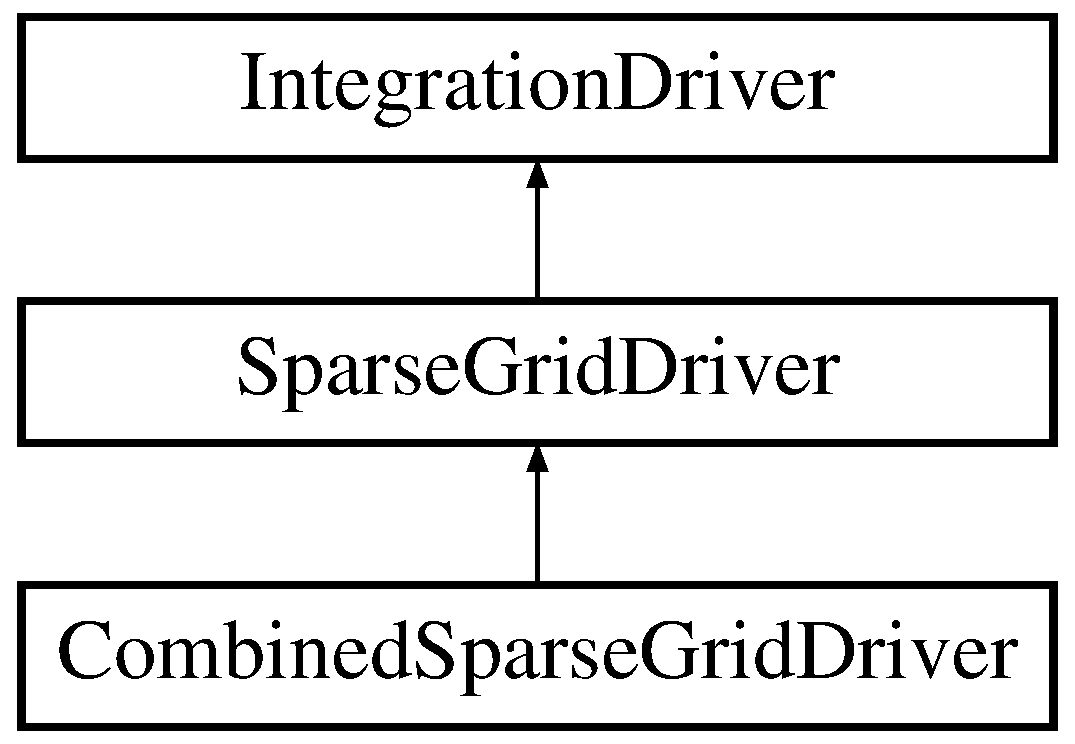
\includegraphics[height=3.000000cm]{classPecos_1_1CombinedSparseGridDriver}
\end{center}
\end{figure}
\subsection*{Public Member Functions}
\begin{DoxyCompactItemize}
\item 
\hyperlink{classPecos_1_1CombinedSparseGridDriver_a1a2f2942af7572d7cec131ac5a963742}{Combined\+Sparse\+Grid\+Driver} ()\label{classPecos_1_1CombinedSparseGridDriver_a1a2f2942af7572d7cec131ac5a963742}

\begin{DoxyCompactList}\small\item\em default constructor \end{DoxyCompactList}\item 
\hyperlink{classPecos_1_1CombinedSparseGridDriver_a88099e5082cd833f8eef69a82756e789}{Combined\+Sparse\+Grid\+Driver} (unsigned short ssg\+\_\+level, const Real\+Vector \&dim\+\_\+pref=Real\+Vector(), short \hyperlink{classPecos_1_1SparseGridDriver_a6f9061513ba25c62ee7a49b0d5da42cc}{growth\+\_\+rate}=M\+O\+D\+E\+R\+A\+T\+E\+\_\+\+R\+E\+S\+T\+R\+I\+C\+T\+E\+D\+\_\+\+G\+R\+O\+W\+TH, short refine\+\_\+control=N\+O\+\_\+\+C\+O\+N\+T\+R\+OL)\label{classPecos_1_1CombinedSparseGridDriver_a88099e5082cd833f8eef69a82756e789}

\begin{DoxyCompactList}\small\item\em constructor \end{DoxyCompactList}\item 
\hyperlink{classPecos_1_1CombinedSparseGridDriver_a4abc6da7da118b54bfb87d7b6af66584}{$\sim$\+Combined\+Sparse\+Grid\+Driver} ()\label{classPecos_1_1CombinedSparseGridDriver_a4abc6da7da118b54bfb87d7b6af66584}

\begin{DoxyCompactList}\small\item\em destructor \end{DoxyCompactList}\item 
void \hyperlink{classPecos_1_1CombinedSparseGridDriver_a66d564a1e3e1b33220a43d2e2629aace}{compute\+\_\+grid} (Real\+Matrix \&variable\+\_\+sets)\label{classPecos_1_1CombinedSparseGridDriver_a66d564a1e3e1b33220a43d2e2629aace}

\begin{DoxyCompactList}\small\item\em compute scaled variable and weight sets for the T\+PQ grid \end{DoxyCompactList}\item 
int \hyperlink{classPecos_1_1CombinedSparseGridDriver_a4b04c73f01f5eb9e6171305141eb1f73}{grid\+\_\+size} ()\label{classPecos_1_1CombinedSparseGridDriver_a4b04c73f01f5eb9e6171305141eb1f73}

\begin{DoxyCompactList}\small\item\em compute (if update\+Grid\+Size) and return number of collocation points with duplicates removed \end{DoxyCompactList}\item 
void \hyperlink{classPecos_1_1CombinedSparseGridDriver_a875c01d83eb38586e43712a94e713312}{reinterpolated\+\_\+tensor\+\_\+grid} (const U\+Short\+Array \&lev\+\_\+index, const Sizet\+List \&reinterp\+\_\+indices)\label{classPecos_1_1CombinedSparseGridDriver_a875c01d83eb38586e43712a94e713312}

\begin{DoxyCompactList}\small\item\em computes and stores data for reinterpolation of covariance on a higher-\/order tensor grid \end{DoxyCompactList}\item 
void \hyperlink{classPecos_1_1CombinedSparseGridDriver_a4a1a63a0f30824fcd233da026bdebef6}{initialize\+\_\+grid} (const std\+::vector$<$ \hyperlink{classPecos_1_1BasisPolynomial}{Basis\+Polynomial} $>$ \&poly\+\_\+basis)\label{classPecos_1_1CombinedSparseGridDriver_a4a1a63a0f30824fcd233da026bdebef6}

\begin{DoxyCompactList}\small\item\em initialize all sparse grid settings (distribution params already set within poly\+\_\+basis) \end{DoxyCompactList}\item 
void \hyperlink{classPecos_1_1CombinedSparseGridDriver_aeae6e6d94a2e3e77d612eee151c77799}{store\+\_\+grid} (size\+\_\+t index=\+\_\+\+N\+P\+OS)\label{classPecos_1_1CombinedSparseGridDriver_aeae6e6d94a2e3e77d612eee151c77799}

\begin{DoxyCompactList}\small\item\em store configuration settings for the current grid before advancing to the next settings within a prescribed grid sequence (default is push\+\_\+back) \end{DoxyCompactList}\item 
void \hyperlink{classPecos_1_1CombinedSparseGridDriver_a31ba839ff630bbc25292b448fff38a73}{restore\+\_\+grid} (size\+\_\+t index=\+\_\+\+N\+P\+OS)\label{classPecos_1_1CombinedSparseGridDriver_a31ba839ff630bbc25292b448fff38a73}

\begin{DoxyCompactList}\small\item\em restore configuration settings from a previously stored grid \end{DoxyCompactList}\item 
void \hyperlink{classPecos_1_1CombinedSparseGridDriver_a93215ecdfbc51b7c45998fa4d65fc7fd}{remove\+\_\+stored\+\_\+grid} (size\+\_\+t index=\+\_\+\+N\+P\+OS)\label{classPecos_1_1CombinedSparseGridDriver_a93215ecdfbc51b7c45998fa4d65fc7fd}

\begin{DoxyCompactList}\small\item\em remove configuration settings for a stored grid (default is pop\+\_\+back) \end{DoxyCompactList}\item 
void \hyperlink{classPecos_1_1CombinedSparseGridDriver_ae4337960917eda26a5672e5c6afbb62a}{clear\+\_\+stored} ()\label{classPecos_1_1CombinedSparseGridDriver_ae4337960917eda26a5672e5c6afbb62a}

\begin{DoxyCompactList}\small\item\em clear stored grid settings following their usage/combination \end{DoxyCompactList}\item 
size\+\_\+t \hyperlink{classPecos_1_1CombinedSparseGridDriver_a6edda8aad31eb8a64e180e6a76a6e0e9}{maximal\+\_\+grid} () const \label{classPecos_1_1CombinedSparseGridDriver_a6edda8aad31eb8a64e180e6a76a6e0e9}

\begin{DoxyCompactList}\small\item\em return the index of the maximal stored grid state (\+\_\+\+N\+P\+OS if the current unstored grid state) \end{DoxyCompactList}\item 
void \hyperlink{classPecos_1_1CombinedSparseGridDriver_ae42d43e21fe55d5b6cca7edf86e54818}{swap\+\_\+grid} (size\+\_\+t index)\label{classPecos_1_1CombinedSparseGridDriver_ae42d43e21fe55d5b6cca7edf86e54818}

\begin{DoxyCompactList}\small\item\em swap settings between the current grid and the stored grid identified by index \end{DoxyCompactList}\item 
void \hyperlink{classPecos_1_1CombinedSparseGridDriver_a059e9e1e03a5cd29771d369b76311261}{initialize\+\_\+sets} ()\label{classPecos_1_1CombinedSparseGridDriver_a059e9e1e03a5cd29771d369b76311261}

\begin{DoxyCompactList}\small\item\em initializes old/active/evaluation sets for use within the generalized sparse grid procedure \end{DoxyCompactList}\item 
void \hyperlink{classPecos_1_1CombinedSparseGridDriver_a99c17efb3a8e873b7708652cc1787370}{push\+\_\+trial\+\_\+set} (const U\+Short\+Array \&set)\label{classPecos_1_1CombinedSparseGridDriver_a99c17efb3a8e873b7708652cc1787370}

\begin{DoxyCompactList}\small\item\em update smolyak\+Multi\+Index with a new trial set for use within the generalized sparse grid procedure \end{DoxyCompactList}\item 
void \hyperlink{classPecos_1_1CombinedSparseGridDriver_ad9648693eacbe856825d2c78b73a3301}{restore\+\_\+set} ()\label{classPecos_1_1CombinedSparseGridDriver_ad9648693eacbe856825d2c78b73a3301}

\begin{DoxyCompactList}\small\item\em update colloc\+Key, colloc\+Indices, and unique\+Index\+Mapping based on restoration of previous trial to smolyak\+Multi\+Index \end{DoxyCompactList}\item 
void \hyperlink{classPecos_1_1CombinedSparseGridDriver_a392163a55c3c5c2b4357b5490009df62}{compute\+\_\+trial\+\_\+grid} (Real\+Matrix \&var\+\_\+sets)\label{classPecos_1_1CombinedSparseGridDriver_a392163a55c3c5c2b4357b5490009df62}

\begin{DoxyCompactList}\small\item\em computes the tensor grid for the index set from \hyperlink{classPecos_1_1CombinedSparseGridDriver_a99c17efb3a8e873b7708652cc1787370}{push\+\_\+trial\+\_\+set()} \end{DoxyCompactList}\item 
void \hyperlink{classPecos_1_1CombinedSparseGridDriver_a92b2604a79028bec35c176aee27e56bb}{pop\+\_\+trial\+\_\+set} ()\label{classPecos_1_1CombinedSparseGridDriver_a92b2604a79028bec35c176aee27e56bb}

\begin{DoxyCompactList}\small\item\em remove the previously pushed trial set from smolyak\+Multi\+Index during the course of the generalized sparse grid procedure \end{DoxyCompactList}\item 
void \hyperlink{classPecos_1_1CombinedSparseGridDriver_a9719b2ab5ff3d7f099fe721a2d7fc6b0}{merge\+\_\+set} ()\label{classPecos_1_1CombinedSparseGridDriver_a9719b2ab5ff3d7f099fe721a2d7fc6b0}

\begin{DoxyCompactList}\small\item\em merge reference sets with trial set and update reference set \end{DoxyCompactList}\item 
void \hyperlink{classPecos_1_1CombinedSparseGridDriver_a07e01bf89eb07535ea78132b8d533088}{finalize\+\_\+sets} (bool output\+\_\+sets, bool converged\+\_\+within\+\_\+tol)\label{classPecos_1_1CombinedSparseGridDriver_a07e01bf89eb07535ea78132b8d533088}

\begin{DoxyCompactList}\small\item\em accept all remaining trial sets within the generalized sparse grid procedure \end{DoxyCompactList}\item 
void \hyperlink{classPecos_1_1CombinedSparseGridDriver_a7b4ed98b79fff649e6f66629f8356542}{update\+\_\+reference} ()\label{classPecos_1_1CombinedSparseGridDriver_a7b4ed98b79fff649e6f66629f8356542}

\begin{DoxyCompactList}\small\item\em update smolyak\+Coeffs\+Ref and type\{1,2\}Weight\+Sets\+Ref for use within the generalized sparse grid procedure \end{DoxyCompactList}\item 
const U\+Short\+Array \& \hyperlink{classPecos_1_1CombinedSparseGridDriver_a5c92e49dbfbcfa5b0d1523ed254b4d76}{trial\+\_\+set} () const \label{classPecos_1_1CombinedSparseGridDriver_a5c92e49dbfbcfa5b0d1523ed254b4d76}

\begin{DoxyCompactList}\small\item\em return trial\+Set \end{DoxyCompactList}\item 
int \hyperlink{classPecos_1_1CombinedSparseGridDriver_a3d8e458c7cf95eae26aa53a738844d89}{unique\+\_\+trial\+\_\+points} () const \label{classPecos_1_1CombinedSparseGridDriver_a3d8e458c7cf95eae26aa53a738844d89}

\begin{DoxyCompactList}\small\item\em return num\+\_\+unique2 \end{DoxyCompactList}\item 
void \hyperlink{classPecos_1_1CombinedSparseGridDriver_af2bf445b9a8d1f418dc3519a3305b05f}{compute\+\_\+grid\+\_\+increment} (Real\+Matrix \&var\+\_\+sets)\label{classPecos_1_1CombinedSparseGridDriver_af2bf445b9a8d1f418dc3519a3305b05f}

\begin{DoxyCompactList}\small\item\em computes tensor grids for new index sets due to an isotropic/anisotropic refinement \end{DoxyCompactList}\item 
void \hyperlink{classPecos_1_1CombinedSparseGridDriver_ae5bcc14a0e7bb726d5280c3dd10e6c98}{print\+\_\+smolyak\+\_\+multi\+\_\+index} () const \label{classPecos_1_1CombinedSparseGridDriver_ae5bcc14a0e7bb726d5280c3dd10e6c98}

\begin{DoxyCompactList}\small\item\em print smolyak\+Multi\+Index \end{DoxyCompactList}\item 
void \hyperlink{classPecos_1_1CombinedSparseGridDriver_a84e051bd519c215c99c164f6a024171e}{initialize\+\_\+grid} (unsigned short ssg\+\_\+level, const Real\+Vector \&dim\+\_\+pref, const Short\+Array \&u\+\_\+types, const \hyperlink{classPecos_1_1ExpansionConfigOptions}{Expansion\+Config\+Options} \&ec\+\_\+options, \hyperlink{classPecos_1_1BasisConfigOptions}{Basis\+Config\+Options} \&bc\+\_\+options, short \hyperlink{classPecos_1_1SparseGridDriver_a6f9061513ba25c62ee7a49b0d5da42cc}{growth\+\_\+rate}=M\+O\+D\+E\+R\+A\+T\+E\+\_\+\+R\+E\+S\+T\+R\+I\+C\+T\+E\+D\+\_\+\+G\+R\+O\+W\+TH, bool track\+\_\+colloc=false, bool track\+\_\+uniq\+\_\+prod\+\_\+wts=true)\label{classPecos_1_1CombinedSparseGridDriver_a84e051bd519c215c99c164f6a024171e}

\begin{DoxyCompactList}\small\item\em initialize all sparse grid settings except for distribution params \end{DoxyCompactList}\item 
void \hyperlink{classPecos_1_1CombinedSparseGridDriver_a4ad5b25d8f7fff7f15a18e45666a3c9c}{assign\+\_\+smolyak\+\_\+arrays} ()\label{classPecos_1_1CombinedSparseGridDriver_a4ad5b25d8f7fff7f15a18e45666a3c9c}

\begin{DoxyCompactList}\small\item\em overloaded form initializes smolyak\+Multi\+Index and smolyak\+Coeffs \end{DoxyCompactList}\item 
void \hyperlink{classPecos_1_1CombinedSparseGridDriver_a2feef60ddf8417a976c8d98a78f8644d}{assign\+\_\+smolyak\+\_\+arrays} (U\+Short2\+D\+Array \&multi\+\_\+index, Int\+Array \&coeffs)\label{classPecos_1_1CombinedSparseGridDriver_a2feef60ddf8417a976c8d98a78f8644d}

\begin{DoxyCompactList}\small\item\em initialize Smolyak multi-\/index (index sets defining the set of tensor products) and Smolyak combinatorial coefficients using an isotropic or anisotropic index set constraint. For anisotropic, webbur\+::sgmga\+\_\+vcn\+\_\+$\ast$ functions are used to compute index sets satisfying the anisotropic index set constraint, along with their corresponding coefficients. \end{DoxyCompactList}\item 
void \hyperlink{classPecos_1_1CombinedSparseGridDriver_ab185944e4f8d69104f77ed055f9d49f8}{update\+\_\+smolyak\+\_\+coefficients} (size\+\_\+t start\+\_\+index)\label{classPecos_1_1CombinedSparseGridDriver_ab185944e4f8d69104f77ed055f9d49f8}

\begin{DoxyCompactList}\small\item\em overloaded form updates smolyak\+Coeffs from smolyak\+Multi\+Index \end{DoxyCompactList}\item 
void \hyperlink{classPecos_1_1CombinedSparseGridDriver_abad795e198f5aca178a132094cf7b99c}{update\+\_\+smolyak\+\_\+coefficients} (size\+\_\+t start\+\_\+index, const U\+Short2\+D\+Array \&multi\+\_\+index, Int\+Array \&coeffs)\label{classPecos_1_1CombinedSparseGridDriver_abad795e198f5aca178a132094cf7b99c}

\begin{DoxyCompactList}\small\item\em update the coeffs array based on new trailing index sets within multi\+\_\+index for incrementally generated generalized sparse grids \end{DoxyCompactList}\item 
void \hyperlink{classPecos_1_1CombinedSparseGridDriver_a9d17415950cab71229a9e2968121ff22}{assign\+\_\+collocation\+\_\+key} ()\label{classPecos_1_1CombinedSparseGridDriver_a9d17415950cab71229a9e2968121ff22}

\begin{DoxyCompactList}\small\item\em initialize colloc\+Key from smolyak\+Multi\+Index \end{DoxyCompactList}\item 
void \hyperlink{classPecos_1_1CombinedSparseGridDriver_a73d4f5d5a559d093a42939a3c79b17b5}{update\+\_\+collocation\+\_\+key} (size\+\_\+t start\+\_\+index)\label{classPecos_1_1CombinedSparseGridDriver_a73d4f5d5a559d093a42939a3c79b17b5}

\begin{DoxyCompactList}\small\item\em update colloc\+Key for the trailing index sets within smolyak\+Multi\+Index \end{DoxyCompactList}\item 
void \hyperlink{classPecos_1_1CombinedSparseGridDriver_ad9e72cee34135fb982921365ccd615cd}{assign\+\_\+collocation\+\_\+indices} ()\label{classPecos_1_1CombinedSparseGridDriver_ad9e72cee34135fb982921365ccd615cd}

\begin{DoxyCompactList}\small\item\em initialize colloc\+Indices from colloc\+Key and unique\+Index\+Mapping \end{DoxyCompactList}\item 
void \hyperlink{classPecos_1_1CombinedSparseGridDriver_a87e86b0c9c443b48aa7bba85ace25c4a}{reference\+\_\+unique} (Real\+Matrix \&var\+\_\+sets)\label{classPecos_1_1CombinedSparseGridDriver_a87e86b0c9c443b48aa7bba85ace25c4a}

\begin{DoxyCompactList}\small\item\em define a1\{Points,Type1\+Weights,Type2\+Weights\} based on the reference grid \end{DoxyCompactList}\item 
void \hyperlink{classPecos_1_1CombinedSparseGridDriver_a9db275646d76935f312de585cc032b35}{increment\+\_\+unique} (bool compute\+\_\+a2, bool \hyperlink{classPecos_1_1SparseGridDriver_ab1c5960af8466c6878fe3c35996c0ae3}{update\+\_\+sets}, Real\+Matrix \&var\+\_\+sets)\label{classPecos_1_1CombinedSparseGridDriver_a9db275646d76935f312de585cc032b35}

\begin{DoxyCompactList}\small\item\em define a2\+Points and update colloc\+Indices and unique\+Index\+Mapping for the trailing index set within smolyak\+Multi\+Index \end{DoxyCompactList}\item 
void \hyperlink{classPecos_1_1CombinedSparseGridDriver_a2ecf6a601999eb7a74d549013b13608c}{merge\+\_\+unique} ()\label{classPecos_1_1CombinedSparseGridDriver_a2ecf6a601999eb7a74d549013b13608c}

\begin{DoxyCompactList}\small\item\em update a1\+Points by merging with unique a2\+Points \end{DoxyCompactList}\item 
void \hyperlink{classPecos_1_1CombinedSparseGridDriver_a761c43d3fbea96d3ebcd7858d2a796d5}{finalize\+\_\+unique} (size\+\_\+t start\+\_\+index)\label{classPecos_1_1CombinedSparseGridDriver_a761c43d3fbea96d3ebcd7858d2a796d5}

\begin{DoxyCompactList}\small\item\em apply all remaining trial sets \end{DoxyCompactList}\item 
void {\bfseries compute\+\_\+tensor\+\_\+points\+\_\+weights} (size\+\_\+t start\+\_\+index, size\+\_\+t num\+\_\+indices, Real\+Matrix \&pts, Real\+Vector \&t1\+\_\+wts, Real\+Matrix \&t2\+\_\+wts)\label{classPecos_1_1CombinedSparseGridDriver_ac64547311f87edb09b8a2bc32388c716}

\item 
void {\bfseries assign\+\_\+tensor\+\_\+collocation\+\_\+indices} (size\+\_\+t start\+\_\+index, const Int\+Array \&unique\+\_\+index)\label{classPecos_1_1CombinedSparseGridDriver_a7ab034ce9d7a36d88b540cce76bd9282}

\item 
const U\+Short2\+D\+Array \& \hyperlink{classPecos_1_1CombinedSparseGridDriver_ac2a92a30d8aedcaf8bcae6097915948d}{smolyak\+\_\+multi\+\_\+index} () const \label{classPecos_1_1CombinedSparseGridDriver_ac2a92a30d8aedcaf8bcae6097915948d}

\begin{DoxyCompactList}\small\item\em return smolyak\+Multi\+Index \end{DoxyCompactList}\item 
const Int\+Array \& \hyperlink{classPecos_1_1CombinedSparseGridDriver_a8a02db8b3454c187db2cc6b7f266ec3c}{smolyak\+\_\+coefficients} () const \label{classPecos_1_1CombinedSparseGridDriver_a8a02db8b3454c187db2cc6b7f266ec3c}

\begin{DoxyCompactList}\small\item\em return smolyak\+Coeffs \end{DoxyCompactList}\item 
const Int\+Array \& \hyperlink{classPecos_1_1CombinedSparseGridDriver_a33a5f4fce5d456312c5ecb7579d34795}{smolyak\+\_\+coefficients\+\_\+reference} () const \label{classPecos_1_1CombinedSparseGridDriver_a33a5f4fce5d456312c5ecb7579d34795}

\begin{DoxyCompactList}\small\item\em return smolyak\+Coeffs\+Ref \end{DoxyCompactList}\item 
void \hyperlink{classPecos_1_1CombinedSparseGridDriver_a23ac0b95407480a7249cfc1fbe7a28c1}{track\+\_\+collocation\+\_\+details} (bool track\+\_\+colloc)\label{classPecos_1_1CombinedSparseGridDriver_a23ac0b95407480a7249cfc1fbe7a28c1}

\begin{DoxyCompactList}\small\item\em set track\+Colloc\+Details \end{DoxyCompactList}\item 
bool \hyperlink{classPecos_1_1CombinedSparseGridDriver_a556842b57e24ec3cf901368e19a2d423}{track\+\_\+collocation\+\_\+details} () const \label{classPecos_1_1CombinedSparseGridDriver_a556842b57e24ec3cf901368e19a2d423}

\begin{DoxyCompactList}\small\item\em get track\+Colloc\+Details \end{DoxyCompactList}\item 
void \hyperlink{classPecos_1_1CombinedSparseGridDriver_aa21b9e5a18f0c713987587e7bb88b6de}{track\+\_\+unique\+\_\+product\+\_\+weights} (bool track\+\_\+uniq\+\_\+prod\+\_\+wts)\label{classPecos_1_1CombinedSparseGridDriver_aa21b9e5a18f0c713987587e7bb88b6de}

\begin{DoxyCompactList}\small\item\em set track\+Unique\+Prod\+Weights \end{DoxyCompactList}\item 
bool \hyperlink{classPecos_1_1CombinedSparseGridDriver_ab200b1697f65bab5112a5aeb55825087}{track\+\_\+unique\+\_\+product\+\_\+weights} () const \label{classPecos_1_1CombinedSparseGridDriver_ab200b1697f65bab5112a5aeb55825087}

\begin{DoxyCompactList}\small\item\em get track\+Unique\+Prod\+Weights \end{DoxyCompactList}\item 
const U\+Short3\+D\+Array \& \hyperlink{classPecos_1_1CombinedSparseGridDriver_a7ee1a2b4537ebad12a0ffff2070af78c}{collocation\+\_\+key} () const \label{classPecos_1_1CombinedSparseGridDriver_a7ee1a2b4537ebad12a0ffff2070af78c}

\begin{DoxyCompactList}\small\item\em return colloc\+Key \end{DoxyCompactList}\item 
const Sizet2\+D\+Array \& \hyperlink{classPecos_1_1CombinedSparseGridDriver_af9d9e61e6d7dc9db34323f5a6c7cbd1f}{collocation\+\_\+indices} () const \label{classPecos_1_1CombinedSparseGridDriver_af9d9e61e6d7dc9db34323f5a6c7cbd1f}

\begin{DoxyCompactList}\small\item\em return colloc\+Indices \end{DoxyCompactList}\item 
const Int\+Array \& \hyperlink{classPecos_1_1CombinedSparseGridDriver_a1b2b5d6dd1639a93b360a614f38b8a79}{unique\+\_\+index\+\_\+mapping} () const \label{classPecos_1_1CombinedSparseGridDriver_a1b2b5d6dd1639a93b360a614f38b8a79}

\begin{DoxyCompactList}\small\item\em return unique\+Index\+Mapping \end{DoxyCompactList}\item 
const U\+Short2\+D\+Array \& \hyperlink{classPecos_1_1CombinedSparseGridDriver_a412d778f5f7e6c19c8bca56f877939ee}{stored\+\_\+smolyak\+\_\+multi\+\_\+index} (size\+\_\+t index) const \label{classPecos_1_1CombinedSparseGridDriver_a412d778f5f7e6c19c8bca56f877939ee}

\begin{DoxyCompactList}\small\item\em return stored\+Lev\+Multi\+Index\mbox{[}index\mbox{]} \end{DoxyCompactList}\item 
const Int\+Array \& \hyperlink{classPecos_1_1CombinedSparseGridDriver_ad592da1b660cbe11c9f2b2ee87cca855}{stored\+\_\+smolyak\+\_\+coefficients} (size\+\_\+t index) const \label{classPecos_1_1CombinedSparseGridDriver_ad592da1b660cbe11c9f2b2ee87cca855}

\begin{DoxyCompactList}\small\item\em return stored\+Lev\+Coeffs\mbox{[}index\mbox{]} \end{DoxyCompactList}\item 
const U\+Short3\+D\+Array \& \hyperlink{classPecos_1_1CombinedSparseGridDriver_a3b0e9e8086c8ac111469fa31b92ac8d6}{stored\+\_\+collocation\+\_\+key} (size\+\_\+t index) const \label{classPecos_1_1CombinedSparseGridDriver_a3b0e9e8086c8ac111469fa31b92ac8d6}

\begin{DoxyCompactList}\small\item\em return stored\+Colloc\+Key\mbox{[}index\mbox{]} \end{DoxyCompactList}\item 
const Sizet2\+D\+Array \& \hyperlink{classPecos_1_1CombinedSparseGridDriver_a2a42f69228dffaa10c86995cee0ff3c7}{stored\+\_\+collocation\+\_\+indices} (size\+\_\+t index) const \label{classPecos_1_1CombinedSparseGridDriver_a2a42f69228dffaa10c86995cee0ff3c7}

\begin{DoxyCompactList}\small\item\em return stored\+Colloc\+Indices\mbox{[}index\mbox{]} \end{DoxyCompactList}\item 
const Real\+Vector \& \hyperlink{classPecos_1_1CombinedSparseGridDriver_ae858d8bd4c244a98b0ff43c979b65e69}{type1\+\_\+weight\+\_\+sets} () const \label{classPecos_1_1CombinedSparseGridDriver_ae858d8bd4c244a98b0ff43c979b65e69}

\begin{DoxyCompactList}\small\item\em return type1\+Weight\+Sets \end{DoxyCompactList}\item 
const Real\+Matrix \& \hyperlink{classPecos_1_1CombinedSparseGridDriver_aacf52fa6f04443949a70c62ee3d718f7}{type2\+\_\+weight\+\_\+sets} () const \label{classPecos_1_1CombinedSparseGridDriver_aacf52fa6f04443949a70c62ee3d718f7}

\begin{DoxyCompactList}\small\item\em return type2\+Weight\+Sets \end{DoxyCompactList}\end{DoxyCompactItemize}
\subsection*{Private Member Functions}
\begin{DoxyCompactItemize}
\item 
void \hyperlink{classPecos_1_1CombinedSparseGridDriver_a7480bf1f3fb2c3d37c3e90f397e5c7fd}{update\+\_\+sparse\+\_\+points} (size\+\_\+t start\+\_\+index, int new\+\_\+index\+\_\+offset, const Real\+Matrix \&tensor\+\_\+pts, const Bit\+Array \&is\+\_\+unique, const Int\+Array \&unique\+\_\+index, Real\+Matrix \&new\+\_\+sparse\+\_\+pts)\label{classPecos_1_1CombinedSparseGridDriver_a7480bf1f3fb2c3d37c3e90f397e5c7fd}

\begin{DoxyCompactList}\small\item\em convenience function for updating sparse points from a set of aggregated tensor points \end{DoxyCompactList}\item 
void \hyperlink{classPecos_1_1CombinedSparseGridDriver_adecce15386ed39c559f4db8f09a08c76}{update\+\_\+sparse\+\_\+weights} (size\+\_\+t start\+\_\+index, const Real\+Vector \&tensor\+\_\+t1\+\_\+wts, const Real\+Matrix \&tensor\+\_\+t2\+\_\+wts, const Int\+Array \&unique\+\_\+index, Real\+Vector \&updated\+\_\+t1\+\_\+wts, Real\+Matrix \&updated\+\_\+t2\+\_\+wts)\label{classPecos_1_1CombinedSparseGridDriver_adecce15386ed39c559f4db8f09a08c76}

\begin{DoxyCompactList}\small\item\em convenience function for updating sparse weights from a set of aggregated tensor weights \end{DoxyCompactList}\item 
void \hyperlink{classPecos_1_1CombinedSparseGridDriver_a4816b36ffde1cee6ae79cce69b1fca20}{initialize\+\_\+duplicate\+\_\+tolerance} ()\label{classPecos_1_1CombinedSparseGridDriver_a4816b36ffde1cee6ae79cce69b1fca20}

\begin{DoxyCompactList}\small\item\em set duplicate\+Tol based on the content of colloc\+Rules\+: table lookups will generally be more precise/repeatable than numerically-\/generated rules \end{DoxyCompactList}\item 
void \hyperlink{classPecos_1_1CombinedSparseGridDriver_a3d59b9fb53b300d676f0d92e960cd0da}{initialize\+\_\+rule\+\_\+pointers} ()\label{classPecos_1_1CombinedSparseGridDriver_a3d59b9fb53b300d676f0d92e960cd0da}

\begin{DoxyCompactList}\small\item\em initialize compute1D\{Points,Type1\+Weights,Type2\+Weights\} function pointer arrays for use within webbur\+::sgmg() and webbur\+::sgmga() routines \end{DoxyCompactList}\item 
void \hyperlink{classPecos_1_1CombinedSparseGridDriver_a3f71fb5043e7b955763a076a47ada140}{initialize\+\_\+growth\+\_\+pointers} ()\label{classPecos_1_1CombinedSparseGridDriver_a3f71fb5043e7b955763a076a47ada140}

\begin{DoxyCompactList}\small\item\em initialize level\+Growth\+To\+Order function pointer arrays for use within webbur\+::sgmg() and webbur\+::sgmga() routines \end{DoxyCompactList}\end{DoxyCompactItemize}
\subsection*{Static Private Member Functions}
\begin{DoxyCompactItemize}
\item 
static void \hyperlink{classPecos_1_1CombinedSparseGridDriver_a085247bab449952c1e08f3cb430a9eb4}{basis\+\_\+collocation\+\_\+points} (int order, int index, double $\ast$data)\label{classPecos_1_1CombinedSparseGridDriver_a085247bab449952c1e08f3cb430a9eb4}

\begin{DoxyCompactList}\small\item\em function passed by pointer for computing collocation points for polynomial\+Basis\mbox{[}index\mbox{]} \end{DoxyCompactList}\item 
static void \hyperlink{classPecos_1_1CombinedSparseGridDriver_ae4518865e9bff4753c3548ebc15fc16e}{basis\+\_\+type1\+\_\+collocation\+\_\+weights} (int order, int index, double $\ast$data)\label{classPecos_1_1CombinedSparseGridDriver_ae4518865e9bff4753c3548ebc15fc16e}

\begin{DoxyCompactList}\small\item\em function passed by pointer for computing type 1 collocation weights for polynomial\+Basis\mbox{[}index\mbox{]} \end{DoxyCompactList}\item 
static void \hyperlink{classPecos_1_1CombinedSparseGridDriver_abc415a7cb5d69e669b6979c32a3b1ac4}{basis\+\_\+type2\+\_\+collocation\+\_\+weights} (int order, int index, double $\ast$data)\label{classPecos_1_1CombinedSparseGridDriver_abc415a7cb5d69e669b6979c32a3b1ac4}

\begin{DoxyCompactList}\small\item\em function passed by pointer for computing type 2 collocation weights for polynomial\+Basis\mbox{[}index\mbox{]} \end{DoxyCompactList}\end{DoxyCompactItemize}
\subsection*{Private Attributes}
\begin{DoxyCompactItemize}
\item 
U\+Short2\+D\+Array \hyperlink{classPecos_1_1CombinedSparseGridDriver_a189de9f4451d4da64b46cff2b4b1ba0d}{smolyak\+Multi\+Index}
\begin{DoxyCompactList}\small\item\em num\+Smolyak\+Indices-\/by-\/num\+Vars array for identifying the index to use within the polynomial\+Basis for a particular variable \end{DoxyCompactList}\item 
Int\+Array \hyperlink{classPecos_1_1CombinedSparseGridDriver_a85aa9102e925ab1e812393e2d42c7548}{smolyak\+Coeffs}\label{classPecos_1_1CombinedSparseGridDriver_a85aa9102e925ab1e812393e2d42c7548}

\begin{DoxyCompactList}\small\item\em array of Smolyak combinatorial coefficients, one for each tensor product index set; order is synchronized with smolyak\+Multi\+Index \end{DoxyCompactList}\item 
Int\+Array \hyperlink{classPecos_1_1CombinedSparseGridDriver_a9e7f6850393e6198600679fe06282e6c}{smolyak\+Coeffs\+Ref}\label{classPecos_1_1CombinedSparseGridDriver_a9e7f6850393e6198600679fe06282e6c}

\begin{DoxyCompactList}\small\item\em reference values for the Smolyak combinatorial coefficients; used in incremental approaches that update smolyak\+Coeffs \end{DoxyCompactList}\item 
bool \hyperlink{classPecos_1_1CombinedSparseGridDriver_abaebe18fcf1f074ef835d32d2932139a}{track\+Colloc\+Details}\label{classPecos_1_1CombinedSparseGridDriver_abaebe18fcf1f074ef835d32d2932139a}

\begin{DoxyCompactList}\small\item\em flag controls conditional population of colloc\+Key, colloc\+Indices, colloc\+Pts1D and type\{1,2\}Colloc\+Wts1D \end{DoxyCompactList}\item 
bool \hyperlink{classPecos_1_1CombinedSparseGridDriver_a81de4ed6a93f8aaa1c2ea141253a2d2a}{track\+Unique\+Prod\+Weights}\label{classPecos_1_1CombinedSparseGridDriver_a81de4ed6a93f8aaa1c2ea141253a2d2a}

\begin{DoxyCompactList}\small\item\em flag indicating need to track \{type1,type2\}Weight\+Sets (product weights for each unique grid point) as opposed to relying on collections of 1D weights \end{DoxyCompactList}\item 
U\+Short3\+D\+Array \hyperlink{classPecos_1_1CombinedSparseGridDriver_a7ac9c2c5db5ccae11777de146f4c487c}{colloc\+Key}\label{classPecos_1_1CombinedSparseGridDriver_a7ac9c2c5db5ccae11777de146f4c487c}

\begin{DoxyCompactList}\small\item\em num\+Smolyak\+Indices-\/by-\/num\+Tensor\+Product\+Pts-\/by-\/num\+Vars array for identifying the 1-\/D point indices for sets of tensor-\/product collocation points \end{DoxyCompactList}\item 
Sizet2\+D\+Array \hyperlink{classPecos_1_1CombinedSparseGridDriver_a91e029d1d2775255b8a3a6604cfbe9e3}{colloc\+Indices}\label{classPecos_1_1CombinedSparseGridDriver_a91e029d1d2775255b8a3a6604cfbe9e3}

\begin{DoxyCompactList}\small\item\em num\+Smolyak\+Indices-\/by-\/num\+Tensor\+Product\+Pts array for linking the set of tensor products to the unique collocation points evaluated \end{DoxyCompactList}\item 
U\+Short\+Array \hyperlink{classPecos_1_1CombinedSparseGridDriver_a54f1421879a8436a667a6a4adba11dd0}{trial\+Set}\label{classPecos_1_1CombinedSparseGridDriver_a54f1421879a8436a667a6a4adba11dd0}

\begin{DoxyCompactList}\small\item\em trial evaluation set from \hyperlink{classPecos_1_1CombinedSparseGridDriver_a99c17efb3a8e873b7708652cc1787370}{push\+\_\+trial\+\_\+set()} \end{DoxyCompactList}\item 
U\+Short3\+D\+Array \hyperlink{classPecos_1_1CombinedSparseGridDriver_a217244fba426bff265ede66abaab32f5}{stored\+Lev\+Multi\+Index}\label{classPecos_1_1CombinedSparseGridDriver_a217244fba426bff265ede66abaab32f5}

\begin{DoxyCompactList}\small\item\em stored driver states\+: copies of smolyak\+Multi\+Index \end{DoxyCompactList}\item 
Int2\+D\+Array \hyperlink{classPecos_1_1CombinedSparseGridDriver_a85706753e4a3ddabba327d695082f3a7}{stored\+Lev\+Coeffs}\label{classPecos_1_1CombinedSparseGridDriver_a85706753e4a3ddabba327d695082f3a7}

\begin{DoxyCompactList}\small\item\em stored driver states\+: copies of smolyak\+Coeffs \end{DoxyCompactList}\item 
U\+Short4\+D\+Array \hyperlink{classPecos_1_1CombinedSparseGridDriver_a016b48727139af0e1bf8300e673692da}{stored\+Colloc\+Key}\label{classPecos_1_1CombinedSparseGridDriver_a016b48727139af0e1bf8300e673692da}

\begin{DoxyCompactList}\small\item\em stored driver states\+: copies of colloc\+Key \end{DoxyCompactList}\item 
Sizet3\+D\+Array \hyperlink{classPecos_1_1CombinedSparseGridDriver_a4d08e2c52e9b964b714c4a9e1759d2ce}{stored\+Colloc\+Indices}\label{classPecos_1_1CombinedSparseGridDriver_a4d08e2c52e9b964b714c4a9e1759d2ce}

\begin{DoxyCompactList}\small\item\em stored driver states\+: copies of colloc\+Indices \end{DoxyCompactList}\item 
Real\+Vector \hyperlink{classPecos_1_1CombinedSparseGridDriver_a5f380207cc4a07db88fe31b3a88b6029}{type1\+Weight\+Sets}\label{classPecos_1_1CombinedSparseGridDriver_a5f380207cc4a07db88fe31b3a88b6029}

\begin{DoxyCompactList}\small\item\em the set of type1 weights (for integration of value interpolants) associated with each point in the sparse grid \end{DoxyCompactList}\item 
Real\+Matrix \hyperlink{classPecos_1_1CombinedSparseGridDriver_a30698bb53a106db16591ea9d4cda6bf5}{type2\+Weight\+Sets}\label{classPecos_1_1CombinedSparseGridDriver_a30698bb53a106db16591ea9d4cda6bf5}

\begin{DoxyCompactList}\small\item\em the set of type2 weights (for integration of gradient interpolants) for each derivative component and for each point in the sparse grid \end{DoxyCompactList}\item 
Real\+Vector \hyperlink{classPecos_1_1CombinedSparseGridDriver_aac98bb355513889fb8f596211f05f4bd}{type1\+Weight\+Sets\+Ref}\label{classPecos_1_1CombinedSparseGridDriver_aac98bb355513889fb8f596211f05f4bd}

\begin{DoxyCompactList}\small\item\em reference values for the type1 weights corresponding to the current reference grid; used in incremental approaches that update type1\+Weight\+Sets \end{DoxyCompactList}\item 
Real\+Matrix \hyperlink{classPecos_1_1CombinedSparseGridDriver_a1f0ca6216a4f2b35bef2ba37421780cb}{type2\+Weight\+Sets\+Ref}\label{classPecos_1_1CombinedSparseGridDriver_a1f0ca6216a4f2b35bef2ba37421780cb}

\begin{DoxyCompactList}\small\item\em reference values for the type2 weights corresponding to the current reference grid; used in incremental approaches that update type2\+Weight\+Sets \end{DoxyCompactList}\item 
Real\+Vector\+Array \hyperlink{classPecos_1_1CombinedSparseGridDriver_a2156536b40c41239c3a68b7e13cbc318}{stored\+Type1\+Weight\+Sets}\label{classPecos_1_1CombinedSparseGridDriver_a2156536b40c41239c3a68b7e13cbc318}

\begin{DoxyCompactList}\small\item\em stored driver states\+: copies of type1\+Weight\+Sets \end{DoxyCompactList}\item 
Real\+Matrix\+Array \hyperlink{classPecos_1_1CombinedSparseGridDriver_a09205b80e2cad1bcf686460ebd1597b2}{stored\+Type2\+Weight\+Sets}\label{classPecos_1_1CombinedSparseGridDriver_a09205b80e2cad1bcf686460ebd1597b2}

\begin{DoxyCompactList}\small\item\em stored driver states\+: copies of type2\+Weight\+Sets \end{DoxyCompactList}\item 
std\+::vector$<$ Colloc\+Fn\+Ptr $>$ \hyperlink{classPecos_1_1CombinedSparseGridDriver_aceca665b19415378de420f29a000d801}{compute1\+D\+Points}\label{classPecos_1_1CombinedSparseGridDriver_aceca665b19415378de420f29a000d801}

\begin{DoxyCompactList}\small\item\em array of pointers to collocation point evaluation functions \end{DoxyCompactList}\item 
std\+::vector$<$ Colloc\+Fn\+Ptr $>$ \hyperlink{classPecos_1_1CombinedSparseGridDriver_a9e24ca931d6591003fef704629d18f42}{compute1\+D\+Type1\+Weights}\label{classPecos_1_1CombinedSparseGridDriver_a9e24ca931d6591003fef704629d18f42}

\begin{DoxyCompactList}\small\item\em array of pointers to type1 collocation weight evaluation functions \end{DoxyCompactList}\item 
std\+::vector$<$ Lev\+Grw\+Ord\+Fn\+Ptr $>$ \hyperlink{classPecos_1_1CombinedSparseGridDriver_afe808947f36b10cae8286885e1fefdfb}{level\+Growth\+To\+Order}\label{classPecos_1_1CombinedSparseGridDriver_afe808947f36b10cae8286885e1fefdfb}

\begin{DoxyCompactList}\small\item\em array of pointers to webbur\+::level\+\_\+to\+\_\+growth functions \end{DoxyCompactList}\item 
Int\+Array \hyperlink{classPecos_1_1CombinedSparseGridDriver_ae4e534b34b8e3d15b82aeb3de346aadc}{unique\+Index\+Mapping}\label{classPecos_1_1CombinedSparseGridDriver_ae4e534b34b8e3d15b82aeb3de346aadc}

\begin{DoxyCompactList}\small\item\em output from sgmga\+\_\+unique\+\_\+index() \end{DoxyCompactList}\item 
Real \hyperlink{classPecos_1_1CombinedSparseGridDriver_a1a80ea24ac69de0a5a92786ad3c891bd}{duplicate\+Tol}\label{classPecos_1_1CombinedSparseGridDriver_a1a80ea24ac69de0a5a92786ad3c891bd}

\begin{DoxyCompactList}\small\item\em duplication tolerance used in sgmga routines \end{DoxyCompactList}\item 
int \hyperlink{classPecos_1_1CombinedSparseGridDriver_a17af4b7ca6a7725086ccb552a185cea2}{num\+Unique1}\label{classPecos_1_1CombinedSparseGridDriver_a17af4b7ca6a7725086ccb552a185cea2}

\begin{DoxyCompactList}\small\item\em number of unique points in set 1 (reference) \end{DoxyCompactList}\item 
int \hyperlink{classPecos_1_1CombinedSparseGridDriver_a202934a96e748245b16a4b5927466061}{num\+Unique2}\label{classPecos_1_1CombinedSparseGridDriver_a202934a96e748245b16a4b5927466061}

\begin{DoxyCompactList}\small\item\em number of unique points in set 2 (increment) \end{DoxyCompactList}\item 
Real\+Vector \hyperlink{classPecos_1_1CombinedSparseGridDriver_a3488da3050b7533f7679cbd1cc13faa9}{z\+Vec}\label{classPecos_1_1CombinedSparseGridDriver_a3488da3050b7533f7679cbd1cc13faa9}

\begin{DoxyCompactList}\small\item\em random vector used within sgmgg for sorting \end{DoxyCompactList}\item 
Real\+Vector \hyperlink{classPecos_1_1CombinedSparseGridDriver_a4924cc208fff080746a7538a022a10be}{r1\+Vec}\label{classPecos_1_1CombinedSparseGridDriver_a4924cc208fff080746a7538a022a10be}

\begin{DoxyCompactList}\small\item\em distance values for sorting in set 1 (reference) \end{DoxyCompactList}\item 
Real\+Vector \hyperlink{classPecos_1_1CombinedSparseGridDriver_a5d12fe02987f9013890917c00416f346}{r2\+Vec}\label{classPecos_1_1CombinedSparseGridDriver_a5d12fe02987f9013890917c00416f346}

\begin{DoxyCompactList}\small\item\em distance values for sorting in set 2 (increment) \end{DoxyCompactList}\item 
Real\+Matrix \hyperlink{classPecos_1_1CombinedSparseGridDriver_a1b34c4c587d4fa71d9a787818fd1b096}{a1\+Points}\label{classPecos_1_1CombinedSparseGridDriver_a1b34c4c587d4fa71d9a787818fd1b096}

\begin{DoxyCompactList}\small\item\em array of collocation points in set 1 (reference) \end{DoxyCompactList}\item 
Real\+Matrix \hyperlink{classPecos_1_1CombinedSparseGridDriver_a00776b02c47d3167bfc4f40df848d843}{a2\+Points}\label{classPecos_1_1CombinedSparseGridDriver_a00776b02c47d3167bfc4f40df848d843}

\begin{DoxyCompactList}\small\item\em array of collocation points in set 2 (increment) \end{DoxyCompactList}\item 
Real\+Vector \hyperlink{classPecos_1_1CombinedSparseGridDriver_ad85e729deb4c8a70b933eb53e3804d64}{a1\+Type1\+Weights}\label{classPecos_1_1CombinedSparseGridDriver_ad85e729deb4c8a70b933eb53e3804d64}

\begin{DoxyCompactList}\small\item\em vector of type1 weights in set 1 (reference) \end{DoxyCompactList}\item 
Real\+Matrix \hyperlink{classPecos_1_1CombinedSparseGridDriver_a28281e426ece80571949cd724e291315}{a1\+Type2\+Weights}\label{classPecos_1_1CombinedSparseGridDriver_a28281e426ece80571949cd724e291315}

\begin{DoxyCompactList}\small\item\em matrix of type2 weights in set 1 (reference) \end{DoxyCompactList}\item 
Real\+Vector \hyperlink{classPecos_1_1CombinedSparseGridDriver_afec3beee6f5e73b3caf88b654c7aad87}{a2\+Type1\+Weights}\label{classPecos_1_1CombinedSparseGridDriver_afec3beee6f5e73b3caf88b654c7aad87}

\begin{DoxyCompactList}\small\item\em vector of type1 weights in set 2 (increment) \end{DoxyCompactList}\item 
Real\+Matrix \hyperlink{classPecos_1_1CombinedSparseGridDriver_acbf578a52f419b34f44a61a0bdb82111}{a2\+Type2\+Weights}\label{classPecos_1_1CombinedSparseGridDriver_acbf578a52f419b34f44a61a0bdb82111}

\begin{DoxyCompactList}\small\item\em matrix of type2 weights in set 2 (increment) \end{DoxyCompactList}\item 
Int\+Array \hyperlink{classPecos_1_1CombinedSparseGridDriver_a01105153b0232b8b5c9e190ecece5e90}{sort\+Index1}\label{classPecos_1_1CombinedSparseGridDriver_a01105153b0232b8b5c9e190ecece5e90}

\begin{DoxyCompactList}\small\item\em ascending sort index for set 1 (reference) \end{DoxyCompactList}\item 
Int\+Array \hyperlink{classPecos_1_1CombinedSparseGridDriver_aba180f01abdd3fc7d200630ace4b0a74}{sort\+Index2}\label{classPecos_1_1CombinedSparseGridDriver_aba180f01abdd3fc7d200630ace4b0a74}

\begin{DoxyCompactList}\small\item\em ascending sort index for set 2 (increment) \end{DoxyCompactList}\item 
Int\+Array \hyperlink{classPecos_1_1CombinedSparseGridDriver_a042d0898a71b7ef73e7569addacddca7}{unique\+Set1}\label{classPecos_1_1CombinedSparseGridDriver_a042d0898a71b7ef73e7569addacddca7}

\begin{DoxyCompactList}\small\item\em index within a1 (reference set) of unique points \end{DoxyCompactList}\item 
Int\+Array \hyperlink{classPecos_1_1CombinedSparseGridDriver_a38fa3e0f8aef40bae0a33fd9711a89a2}{unique\+Set2}\label{classPecos_1_1CombinedSparseGridDriver_a38fa3e0f8aef40bae0a33fd9711a89a2}

\begin{DoxyCompactList}\small\item\em index within a2 (increment set) of unique points \end{DoxyCompactList}\item 
Int\+Array \hyperlink{classPecos_1_1CombinedSparseGridDriver_a7607c386a6c08f235bdfad69c0937f7f}{unique\+Index1}\label{classPecos_1_1CombinedSparseGridDriver_a7607c386a6c08f235bdfad69c0937f7f}

\begin{DoxyCompactList}\small\item\em index within unique\+Set1 corresponding to all of a1 \end{DoxyCompactList}\item 
Int\+Array \hyperlink{classPecos_1_1CombinedSparseGridDriver_a577f382112f6dd0559474bb9cb71a015}{unique\+Index2}\label{classPecos_1_1CombinedSparseGridDriver_a577f382112f6dd0559474bb9cb71a015}

\begin{DoxyCompactList}\small\item\em index within unique\+Set2 corresponding to all of a2 \end{DoxyCompactList}\item 
Bit\+Array \hyperlink{classPecos_1_1CombinedSparseGridDriver_aeecc374a27a3acd87b5dfc42e81ca511}{is\+Unique1}\label{classPecos_1_1CombinedSparseGridDriver_aeecc374a27a3acd87b5dfc42e81ca511}

\begin{DoxyCompactList}\small\item\em key to unique points in set 1 (reference) \end{DoxyCompactList}\item 
Bit\+Array \hyperlink{classPecos_1_1CombinedSparseGridDriver_a7716c733bc8fff78b4a7feefbf1c4b29}{is\+Unique2}\label{classPecos_1_1CombinedSparseGridDriver_a7716c733bc8fff78b4a7feefbf1c4b29}

\begin{DoxyCompactList}\small\item\em key to unique points in set 2 (increment) \end{DoxyCompactList}\end{DoxyCompactItemize}
\subsection*{Static Private Attributes}
\begin{DoxyCompactItemize}
\item 
static \hyperlink{classPecos_1_1CombinedSparseGridDriver}{Combined\+Sparse\+Grid\+Driver} $\ast$ \hyperlink{classPecos_1_1CombinedSparseGridDriver_ab59a7e6f0acf79265a38279b0d4350d0}{sgd\+Instance}
\begin{DoxyCompactList}\small\item\em pointer to instance of this class for use in static member functions \end{DoxyCompactList}\end{DoxyCompactItemize}
\subsection*{Additional Inherited Members}


\subsection{Detailed Description}
Derived integration driver class that generates N-\/dimensional Smolyak sparse grids for numerical evaluation of expectation integrals over independent standard random variables. 

This class is used by Dakota\+::\+Non\+D\+Sparse\+Grid, but could also be used for general numerical integration of moments. It employs 1-\/D Clenshaw-\/\+Curtis, Newton-\/\+Cotes, and Gaussian quadrature rules within Smolyak sparse grids. 

\subsection{Member Data Documentation}
\index{Pecos\+::\+Combined\+Sparse\+Grid\+Driver@{Pecos\+::\+Combined\+Sparse\+Grid\+Driver}!sgd\+Instance@{sgd\+Instance}}
\index{sgd\+Instance@{sgd\+Instance}!Pecos\+::\+Combined\+Sparse\+Grid\+Driver@{Pecos\+::\+Combined\+Sparse\+Grid\+Driver}}
\subsubsection[{\texorpdfstring{sgd\+Instance}{sgdInstance}}]{\setlength{\rightskip}{0pt plus 5cm}{\bf Combined\+Sparse\+Grid\+Driver} $\ast$ sgd\+Instance\hspace{0.3cm}{\ttfamily [static]}, {\ttfamily [private]}}\label{classPecos_1_1CombinedSparseGridDriver_ab59a7e6f0acf79265a38279b0d4350d0}


pointer to instance of this class for use in static member functions 

initialize static member pointer to active driver instance 

Referenced by Combined\+Sparse\+Grid\+Driver\+::basis\+\_\+collocation\+\_\+points(), Combined\+Sparse\+Grid\+Driver\+::basis\+\_\+type1\+\_\+collocation\+\_\+weights(), Combined\+Sparse\+Grid\+Driver\+::basis\+\_\+type2\+\_\+collocation\+\_\+weights(), Combined\+Sparse\+Grid\+Driver\+::compute\+\_\+grid(), and Combined\+Sparse\+Grid\+Driver\+::grid\+\_\+size().

\index{Pecos\+::\+Combined\+Sparse\+Grid\+Driver@{Pecos\+::\+Combined\+Sparse\+Grid\+Driver}!smolyak\+Multi\+Index@{smolyak\+Multi\+Index}}
\index{smolyak\+Multi\+Index@{smolyak\+Multi\+Index}!Pecos\+::\+Combined\+Sparse\+Grid\+Driver@{Pecos\+::\+Combined\+Sparse\+Grid\+Driver}}
\subsubsection[{\texorpdfstring{smolyak\+Multi\+Index}{smolyakMultiIndex}}]{\setlength{\rightskip}{0pt plus 5cm}U\+Short2\+D\+Array smolyak\+Multi\+Index\hspace{0.3cm}{\ttfamily [private]}}\label{classPecos_1_1CombinedSparseGridDriver_a189de9f4451d4da64b46cff2b4b1ba0d}


num\+Smolyak\+Indices-\/by-\/num\+Vars array for identifying the index to use within the polynomial\+Basis for a particular variable 

The index sets correspond to j (0-\/based) for use as indices, which are offset from the i indices (1-\/based) normally used in the Smolyak expressions. The indices correspond to levels, one for each anisotropic tensor-\/product grid within a Smolyak recursion. 

Referenced by Combined\+Sparse\+Grid\+Driver\+::assign\+\_\+collocation\+\_\+key(), Combined\+Sparse\+Grid\+Driver\+::assign\+\_\+smolyak\+\_\+arrays(), Combined\+Sparse\+Grid\+Driver\+::finalize\+\_\+sets(), Combined\+Sparse\+Grid\+Driver\+::finalize\+\_\+unique(), Combined\+Sparse\+Grid\+Driver\+::increment\+\_\+unique(), Combined\+Sparse\+Grid\+Driver\+::initialize\+\_\+sets(), Combined\+Sparse\+Grid\+Driver\+::pop\+\_\+trial\+\_\+set(), Combined\+Sparse\+Grid\+Driver\+::print\+\_\+smolyak\+\_\+multi\+\_\+index(), Combined\+Sparse\+Grid\+Driver\+::push\+\_\+trial\+\_\+set(), Combined\+Sparse\+Grid\+Driver\+::reference\+\_\+unique(), Combined\+Sparse\+Grid\+Driver\+::restore\+\_\+grid(), Combined\+Sparse\+Grid\+Driver\+::restore\+\_\+set(), Combined\+Sparse\+Grid\+Driver\+::smolyak\+\_\+multi\+\_\+index(), Combined\+Sparse\+Grid\+Driver\+::store\+\_\+grid(), Combined\+Sparse\+Grid\+Driver\+::swap\+\_\+grid(), Combined\+Sparse\+Grid\+Driver\+::update\+\_\+collocation\+\_\+key(), Combined\+Sparse\+Grid\+Driver\+::update\+\_\+smolyak\+\_\+coefficients(), Combined\+Sparse\+Grid\+Driver\+::update\+\_\+sparse\+\_\+points(), and Combined\+Sparse\+Grid\+Driver\+::update\+\_\+sparse\+\_\+weights().



The documentation for this class was generated from the following files\+:\begin{DoxyCompactItemize}
\item 
Combined\+Sparse\+Grid\+Driver.\+hpp\item 
Combined\+Sparse\+Grid\+Driver.\+cpp\end{DoxyCompactItemize}

\section{Compressed\+Sensing\+Options Class Reference}
\label{classPecos_1_1CompressedSensingOptions}\index{Compressed\+Sensing\+Options@{Compressed\+Sensing\+Options}}


Specify a set of options for using the \hyperlink{classPecos_1_1CompressedSensingTool}{Compressed\+Sensing\+Tool}.  


\subsection*{Public Member Functions}
\begin{DoxyCompactItemize}
\item 
void {\bfseries print} ()\label{classPecos_1_1CompressedSensingOptions_a388f572c62279f839ee138a9afbdeeb5}

\item 
\hyperlink{classPecos_1_1CompressedSensingOptions}{Compressed\+Sensing\+Options} \& {\bfseries operator=} (const \hyperlink{classPecos_1_1CompressedSensingOptions}{Compressed\+Sensing\+Options} \&source)\label{classPecos_1_1CompressedSensingOptions_af453c626039ee0fc37039f9f33543ba9}

\item 
{\bfseries Compressed\+Sensing\+Options} (const \hyperlink{classPecos_1_1CompressedSensingOptions}{Compressed\+Sensing\+Options} \&source)\label{classPecos_1_1CompressedSensingOptions_adc0fc39a0f69e3bfd07f0824711a8c44}

\end{DoxyCompactItemize}
\subsection*{Public Attributes}
\begin{DoxyCompactItemize}
\item 
short \hyperlink{classPecos_1_1CompressedSensingOptions_a3df2a8fab282b8ceac58d1add07afb94}{solver}\label{classPecos_1_1CompressedSensingOptions_a3df2a8fab282b8ceac58d1add07afb94}

\begin{DoxyCompactList}\small\item\em Specify which regression solver to use\+: see pecos\+\_\+global\+\_\+defs. \end{DoxyCompactList}\item 
Real \hyperlink{classPecos_1_1CompressedSensingOptions_a1149f15b677e7a27b720a27b9c0ac5ec}{solver\+Tolerance}\label{classPecos_1_1CompressedSensingOptions_a1149f15b677e7a27b720a27b9c0ac5ec}

\begin{DoxyCompactList}\small\item\em Specify the internal tolerance of the solver. \end{DoxyCompactList}\item 
Real \hyperlink{classPecos_1_1CompressedSensingOptions_a7cd0383f653cbd5fa1542574a226f311}{epsilon}\label{classPecos_1_1CompressedSensingOptions_a7cd0383f653cbd5fa1542574a226f311}

\begin{DoxyCompactList}\small\item\em Specify the residual tolerance of the solver. \end{DoxyCompactList}\item 
Real \hyperlink{classPecos_1_1CompressedSensingOptions_a6e815cecfc8bf0ee83558d5bfd70c2d1}{delta}\label{classPecos_1_1CompressedSensingOptions_a6e815cecfc8bf0ee83558d5bfd70c2d1}

\begin{DoxyCompactList}\small\item\em Specify the regularization parameter value. \end{DoxyCompactList}\item 
int \hyperlink{classPecos_1_1CompressedSensingOptions_a85d28d944a2380ab6f6f0ec5ff01dbda}{max\+Num\+Iterations}\label{classPecos_1_1CompressedSensingOptions_a85d28d944a2380ab6f6f0ec5ff01dbda}

\begin{DoxyCompactList}\small\item\em Specify the maximum number of solver iterations. \end{DoxyCompactList}\item 
bool \hyperlink{classPecos_1_1CompressedSensingOptions_afd70c4df5fec2b0851b2b2534d63b852}{standardize\+Inputs}\label{classPecos_1_1CompressedSensingOptions_afd70c4df5fec2b0851b2b2534d63b852}

\begin{DoxyCompactList}\small\item\em Specify if the inputs need to be standardized. \end{DoxyCompactList}\item 
bool {\bfseries store\+History}\label{classPecos_1_1CompressedSensingOptions_a67af0d64911c811dedcbe56adb978e18}

\item 
Real {\bfseries conjugate\+Gradients\+Tolerance}\label{classPecos_1_1CompressedSensingOptions_a7734271f72c9ee4835861e657cc250f8}

\item 
int \hyperlink{classPecos_1_1CompressedSensingOptions_a1bdcfae3209cbd96db35a2ae356fa15e}{verbosity}\label{classPecos_1_1CompressedSensingOptions_a1bdcfae3209cbd96db35a2ae356fa15e}

\begin{DoxyCompactList}\small\item\em The verbosity level. 0\+: off, 1\+: warnings on, 2\+: all print statements on. \end{DoxyCompactList}\item 
int \hyperlink{classPecos_1_1CompressedSensingOptions_a21e4bfae200b8fda9f18764d3c8a2c88}{num\+Function\+Samples}\label{classPecos_1_1CompressedSensingOptions_a21e4bfae200b8fda9f18764d3c8a2c88}

\begin{DoxyCompactList}\small\item\em The number of function samples used to construct A and B. Used when A contains gradient information. If zero then num\+Function\+Samples = A.\+num\+Rows() \end{DoxyCompactList}\end{DoxyCompactItemize}


\subsection{Detailed Description}
Specify a set of options for using the \hyperlink{classPecos_1_1CompressedSensingTool}{Compressed\+Sensing\+Tool}. 

The documentation for this class was generated from the following file\+:\begin{DoxyCompactItemize}
\item 
Linear\+Solver.\+hpp\end{DoxyCompactItemize}

\section{Compressed\+Sensing\+Tool Class Reference}
\label{classPecos_1_1CompressedSensingTool}\index{Compressed\+Sensing\+Tool@{Compressed\+Sensing\+Tool}}


Tool that implements a number of popular compressed sensing algorithms.  


\subsection*{Public Member Functions}
\begin{DoxyCompactItemize}
\item 
\hyperlink{classPecos_1_1CompressedSensingTool_a91459f946e396f732cda23cdcd100da4}{Compressed\+Sensing\+Tool} ()\label{classPecos_1_1CompressedSensingTool_a91459f946e396f732cda23cdcd100da4}

\begin{DoxyCompactList}\small\item\em Default constructor. \end{DoxyCompactList}\end{DoxyCompactItemize}
\begin{Indent}{\bf Interface tools.}\par
\begin{DoxyCompactItemize}
\item 
void \hyperlink{classPecos_1_1CompressedSensingTool_a0592765825357e99967a93c209e819b8}{solve} (Real\+Matrix \&A, Real\+Matrix \&B, Real\+Matrix\+Array \&solutions, \hyperlink{classPecos_1_1CompressedSensingOptions}{Compressed\+Sensing\+Options} \&opts, Compressed\+Sensing\+Options\+List \&opts\+\_\+list)
\begin{DoxyCompactList}\small\item\em Wrapper to call any of the compressed sensing methods. \end{DoxyCompactList}\item 
void {\bfseries set\+\_\+linear\+\_\+solver} (\hyperlink{classPecos_1_1CompressedSensingOptions}{Compressed\+Sensing\+Options} \&opts)\label{classPecos_1_1CompressedSensingTool_a48546251ce1a9161e5466558a194df7a}

\item 
Linear\+Solver\+\_\+ptr {\bfseries get\+\_\+linear\+\_\+solver} ()\label{classPecos_1_1CompressedSensingTool_a321ce094268110552afd01e28c310bc5}

\end{DoxyCompactItemize}
\end{Indent}
\subsection*{Protected Attributes}
\begin{DoxyCompactItemize}
\item 
Linear\+Solver\+\_\+ptr {\bfseries linear\+Solver\+\_\+}\label{classPecos_1_1CompressedSensingTool_a769e9b3215d849779987b48a8d0322c4}

\end{DoxyCompactItemize}


\subsection{Detailed Description}
Tool that implements a number of popular compressed sensing algorithms. 

\subsection{Member Function Documentation}
\index{Pecos\+::\+Compressed\+Sensing\+Tool@{Pecos\+::\+Compressed\+Sensing\+Tool}!solve@{solve}}
\index{solve@{solve}!Pecos\+::\+Compressed\+Sensing\+Tool@{Pecos\+::\+Compressed\+Sensing\+Tool}}
\subsubsection[{\texorpdfstring{solve(\+Real\+Matrix \&\+A, Real\+Matrix \&\+B, Real\+Matrix\+Array \&solutions, Compressed\+Sensing\+Options \&opts, Compressed\+Sensing\+Options\+List \&opts\+\_\+list)}{solve(RealMatrix &A, RealMatrix &B, RealMatrixArray &solutions, CompressedSensingOptions &opts, CompressedSensingOptionsList &opts_list)}}]{\setlength{\rightskip}{0pt plus 5cm}void solve (
\begin{DoxyParamCaption}
\item[{Real\+Matrix \&}]{A, }
\item[{Real\+Matrix \&}]{B, }
\item[{Real\+Matrix\+Array \&}]{solutions, }
\item[{{\bf Compressed\+Sensing\+Options} \&}]{opts, }
\item[{Compressed\+Sensing\+Options\+List \&}]{opts\+\_\+list}
\end{DoxyParamCaption}
)}\label{classPecos_1_1CompressedSensingTool_a0592765825357e99967a93c209e819b8}


Wrapper to call any of the compressed sensing methods. 


\begin{DoxyParams}{Parameters}
{\em A} & ( M x N ) matrix of the linear system AX=B\\
\hline
{\em B} & ( M x num\+\_\+rhs ) matrix of the linear system AX=B\\
\hline
{\em solutions} & (output) vector containing multiple solutions to AX=B. Each entry in solutions is a ( N x num\+\_\+rhs ) matrix opts.\+solver=LS will return only one solution whilst methods such as O\+MP, L\+A\+RS, and L\+A\+S\+SO will return a history of solutions\\
\hline
{\em opts} & specifies the method options\\
\hline
{\em opts\+\_\+list} & specifies the method options that can be used to reproduce all the solutions found. \\
\hline
\end{DoxyParams}


References Compressed\+Sensing\+Options\+::delta, Compressed\+Sensing\+Options\+::epsilon, Compressed\+Sensing\+Options\+::max\+Num\+Iterations, Compressed\+Sensing\+Options\+::num\+Function\+Samples, Pecos\+::reshape(), Compressed\+Sensing\+Options\+::solver, Compressed\+Sensing\+Options\+::solver\+Tolerance, and Compressed\+Sensing\+Options\+::verbosity.



Referenced by Regress\+Orthog\+Poly\+Approximation\+::compressed\+\_\+sensing().



The documentation for this class was generated from the following files\+:\begin{DoxyCompactItemize}
\item 
Linear\+Solver.\+hpp\item 
Linear\+Solver.\+cpp\end{DoxyCompactItemize}

\section{Cubature\+Driver Class Reference}
\label{classPecos_1_1CubatureDriver}\index{Cubature\+Driver@{Cubature\+Driver}}


Generates N-\/dimensional cubature grids for numerical evaluation of expectation integrals over independent standard random variables.  


Inheritance diagram for Cubature\+Driver\+:\begin{figure}[H]
\begin{center}
\leavevmode
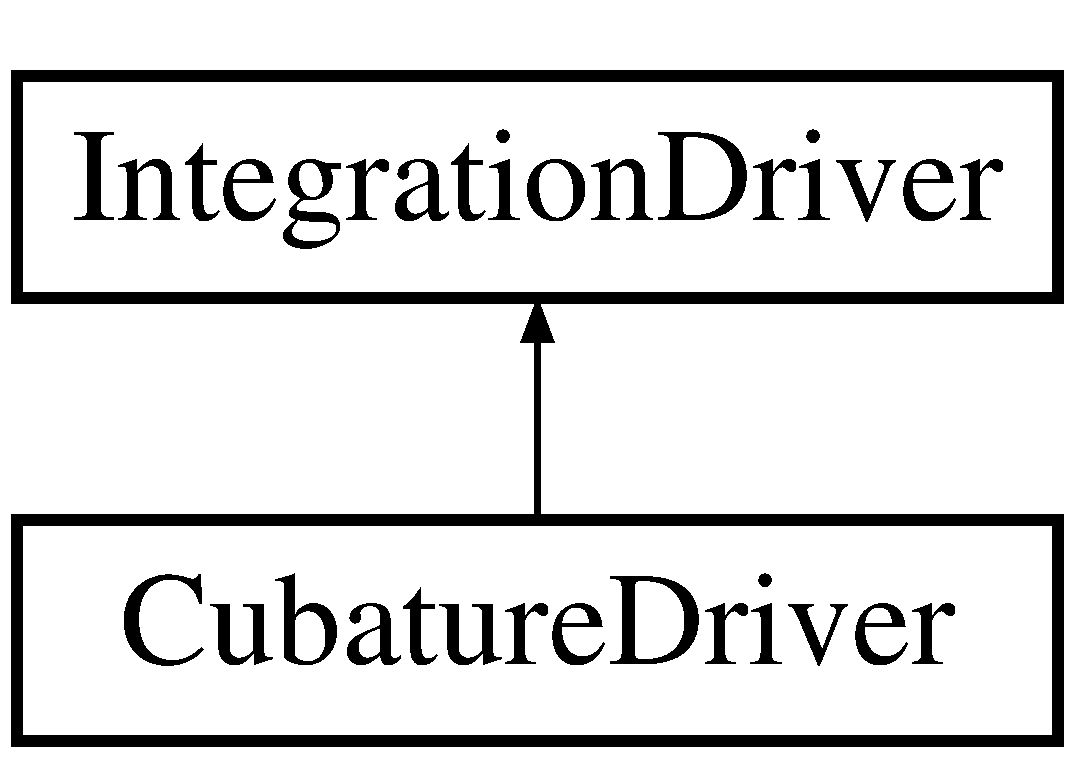
\includegraphics[height=2.000000cm]{classPecos_1_1CubatureDriver}
\end{center}
\end{figure}
\subsection*{Public Member Functions}
\begin{DoxyCompactItemize}
\item 
\hyperlink{classPecos_1_1CubatureDriver_a3ec1c82f25587cdc1174b58950c5c2d2}{Cubature\+Driver} ()\label{classPecos_1_1CubatureDriver_a3ec1c82f25587cdc1174b58950c5c2d2}

\begin{DoxyCompactList}\small\item\em default constructor \end{DoxyCompactList}\item 
\hyperlink{classPecos_1_1CubatureDriver_acc9f0bce593907db9cf90297f1959351}{Cubature\+Driver} (unsigned short \hyperlink{classPecos_1_1CubatureDriver_afcf9a1f723bcb50caf73da3bb31362c4}{integrand\+\_\+order})\label{classPecos_1_1CubatureDriver_acc9f0bce593907db9cf90297f1959351}

\begin{DoxyCompactList}\small\item\em constructor \end{DoxyCompactList}\item 
\hyperlink{classPecos_1_1CubatureDriver_a8c303dc560a8d94efb91548ea015ff2e}{$\sim$\+Cubature\+Driver} ()\label{classPecos_1_1CubatureDriver_a8c303dc560a8d94efb91548ea015ff2e}

\begin{DoxyCompactList}\small\item\em destructor \end{DoxyCompactList}\item 
void \hyperlink{classPecos_1_1CubatureDriver_a779bd2b2a1f6d287983396aa7ce65f69}{initialize\+\_\+grid} (const Short\+Array \&u\+\_\+types, unsigned short order, unsigned short rule)\label{classPecos_1_1CubatureDriver_a779bd2b2a1f6d287983396aa7ce65f69}

\begin{DoxyCompactList}\small\item\em initialize cubature settings except for distribution params \end{DoxyCompactList}\item 
void \hyperlink{classPecos_1_1CubatureDriver_a4a1a63a0f30824fcd233da026bdebef6}{initialize\+\_\+grid} (const std\+::vector$<$ \hyperlink{classPecos_1_1BasisPolynomial}{Basis\+Polynomial} $>$ \&poly\+\_\+basis)\label{classPecos_1_1CubatureDriver_a4a1a63a0f30824fcd233da026bdebef6}

\begin{DoxyCompactList}\small\item\em initialize all cubature settings (distribution params already set within poly\+\_\+basis) \end{DoxyCompactList}\item 
void \hyperlink{classPecos_1_1CubatureDriver_a8ccb22f815295e0cbc3ef645af30ca02}{initialize\+\_\+grid\+\_\+parameters} (const Short\+Array \&u\+\_\+types, const \hyperlink{classPecos_1_1AleatoryDistParams}{Aleatory\+Dist\+Params} \&dp)\label{classPecos_1_1CubatureDriver_a8ccb22f815295e0cbc3ef645af30ca02}

\begin{DoxyCompactList}\small\item\em initialize settings for parameterized cubature rules \end{DoxyCompactList}\item 
void \hyperlink{classPecos_1_1CubatureDriver_afcf9a1f723bcb50caf73da3bb31362c4}{integrand\+\_\+order} (unsigned short order)\label{classPecos_1_1CubatureDriver_afcf9a1f723bcb50caf73da3bb31362c4}

\begin{DoxyCompactList}\small\item\em set integrand\+Order \end{DoxyCompactList}\item 
unsigned short \hyperlink{classPecos_1_1CubatureDriver_a22765dd74a676125244e482f9a6c2f9f}{integrand\+\_\+order} () const \label{classPecos_1_1CubatureDriver_a22765dd74a676125244e482f9a6c2f9f}

\begin{DoxyCompactList}\small\item\em get integrand\+Order \end{DoxyCompactList}\item 
const Real\+Vector \& \hyperlink{classPecos_1_1CubatureDriver_ae858d8bd4c244a98b0ff43c979b65e69}{type1\+\_\+weight\+\_\+sets} () const \label{classPecos_1_1CubatureDriver_ae858d8bd4c244a98b0ff43c979b65e69}

\begin{DoxyCompactList}\small\item\em return type1\+Weight\+Sets \end{DoxyCompactList}\item 
int \hyperlink{classPecos_1_1CubatureDriver_a4b04c73f01f5eb9e6171305141eb1f73}{grid\+\_\+size} ()\label{classPecos_1_1CubatureDriver_a4b04c73f01f5eb9e6171305141eb1f73}

\begin{DoxyCompactList}\small\item\em number of collocation points with duplicates removed \end{DoxyCompactList}\item 
void \hyperlink{classPecos_1_1CubatureDriver_a66d564a1e3e1b33220a43d2e2629aace}{compute\+\_\+grid} (Real\+Matrix \&variable\+\_\+sets)\label{classPecos_1_1CubatureDriver_a66d564a1e3e1b33220a43d2e2629aace}

\begin{DoxyCompactList}\small\item\em compute scaled variable and weight sets for the cubature grid \end{DoxyCompactList}\end{DoxyCompactItemize}
\subsection*{Private Member Functions}
\begin{DoxyCompactItemize}
\item 
bool \hyperlink{classPecos_1_1CubatureDriver_a2f98c02b4c3e1f3253cdec894890bf63}{verify\+\_\+homogeneity} (const Real\+Vector \&params) const \label{classPecos_1_1CubatureDriver_a2f98c02b4c3e1f3253cdec894890bf63}

\begin{DoxyCompactList}\small\item\em verify that all values within params are identical \end{DoxyCompactList}\item 
bool \hyperlink{classPecos_1_1CubatureDriver_af390abf13e45e5633560edce5035c96b}{verify\+\_\+homogeneity} (const Real\+Real\+Map\+Array \&params) const \label{classPecos_1_1CubatureDriver_af390abf13e45e5633560edce5035c96b}

\begin{DoxyCompactList}\small\item\em verify that all vectors within params are identical \end{DoxyCompactList}\item 
void \hyperlink{classPecos_1_1CubatureDriver_a3ffbf2daf7cd6623695e749bf6a7224b}{collocation\+\_\+rule} (unsigned short rule)\label{classPecos_1_1CubatureDriver_a3ffbf2daf7cd6623695e749bf6a7224b}

\begin{DoxyCompactList}\small\item\em size colloc\+Rules and set first entry \end{DoxyCompactList}\end{DoxyCompactItemize}
\subsection*{Private Attributes}
\begin{DoxyCompactItemize}
\item 
unsigned short \hyperlink{classPecos_1_1CubatureDriver_a2daa6f441a3b1848d716e80df5ff2f01}{integrand\+Order}\label{classPecos_1_1CubatureDriver_a2daa6f441a3b1848d716e80df5ff2f01}

\begin{DoxyCompactList}\small\item\em integrand order \end{DoxyCompactList}\item 
int \hyperlink{classPecos_1_1CubatureDriver_ad90387d39d501e7fda7bb777fd5b218f}{num\+Pts}\label{classPecos_1_1CubatureDriver_ad90387d39d501e7fda7bb777fd5b218f}

\begin{DoxyCompactList}\small\item\em the current number of unique points in the grid \end{DoxyCompactList}\item 
bool \hyperlink{classPecos_1_1CubatureDriver_a467d131ddb4afdf1aaf1e51ce80d7c34}{update\+Grid\+Size}\label{classPecos_1_1CubatureDriver_a467d131ddb4afdf1aaf1e51ce80d7c34}

\begin{DoxyCompactList}\small\item\em flag indicating when num\+Pts needs to be recomputed due to an update to the cubature settings \end{DoxyCompactList}\item 
Real\+Vector \hyperlink{classPecos_1_1CubatureDriver_a5f380207cc4a07db88fe31b3a88b6029}{type1\+Weight\+Sets}\label{classPecos_1_1CubatureDriver_a5f380207cc4a07db88fe31b3a88b6029}

\begin{DoxyCompactList}\small\item\em the set of type1 weights (for integration of value interpolants) associated with each point in the \{T\+PQ,S\+SG,Cub\} grid \end{DoxyCompactList}\end{DoxyCompactItemize}
\subsection*{Additional Inherited Members}


\subsection{Detailed Description}
Generates N-\/dimensional cubature grids for numerical evaluation of expectation integrals over independent standard random variables. 

Includes Stroud rules and extensions. This class is used by Dakota\+::\+Non\+D\+Cubature, but could also be used for general numerical integration of moments. 

The documentation for this class was generated from the following files\+:\begin{DoxyCompactItemize}
\item 
Cubature\+Driver.\+hpp\item 
Cubature\+Driver.\+cpp\end{DoxyCompactItemize}

\section{Data\+Transformation Class Reference}
\label{classPecos_1_1DataTransformation}\index{Data\+Transformation@{Data\+Transformation}}


Base class for forward/inverse transformations between time and frequency domain data.  


Inheritance diagram for Data\+Transformation\+:\begin{figure}[H]
\begin{center}
\leavevmode
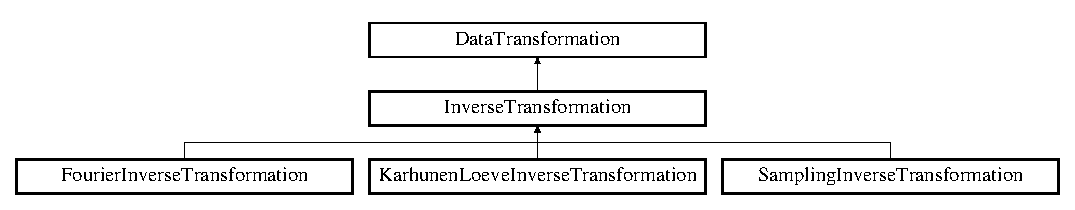
\includegraphics[height=2.372881cm]{classPecos_1_1DataTransformation}
\end{center}
\end{figure}
\subsection*{Public Member Functions}
\begin{DoxyCompactItemize}
\item 
\hyperlink{classPecos_1_1DataTransformation_ac6edfcdb46b6e07c9bdd6869ea407ad8}{Data\+Transformation} ()
\begin{DoxyCompactList}\small\item\em default constructor \end{DoxyCompactList}\item 
\hyperlink{classPecos_1_1DataTransformation_a58ce1cb41e61bc30ebbcc3a80b7a75c6}{Data\+Transformation} (const String \&data\+\_\+trans\+\_\+type)
\begin{DoxyCompactList}\small\item\em standard constructor for envelope \end{DoxyCompactList}\item 
\hyperlink{classPecos_1_1DataTransformation_ad6aff7a1529d9c7b8805587d7ec80a24}{Data\+Transformation} (const \hyperlink{classPecos_1_1DataTransformation}{Data\+Transformation} \&data\+\_\+trans)
\begin{DoxyCompactList}\small\item\em copy constructor \end{DoxyCompactList}\item 
virtual \hyperlink{classPecos_1_1DataTransformation_a11731ed3d0ac8be4aafdbc9b18d84aba}{$\sim$\+Data\+Transformation} ()
\begin{DoxyCompactList}\small\item\em destructor \end{DoxyCompactList}\item 
\hyperlink{classPecos_1_1DataTransformation}{Data\+Transformation} \hyperlink{classPecos_1_1DataTransformation_af090d7f211241ad41f7269f5e653d83c}{operator=} (const \hyperlink{classPecos_1_1DataTransformation}{Data\+Transformation} \&data\+\_\+trans)
\begin{DoxyCompactList}\small\item\em assignment operator \end{DoxyCompactList}\item 
virtual void \hyperlink{classPecos_1_1DataTransformation_aff7310eaa8322a3eccf9815cc7da4a8e}{initialize} (const Real \&total\+\_\+t, const Real \&w\+\_\+bar, size\+\_\+t seed)\label{classPecos_1_1DataTransformation_aff7310eaa8322a3eccf9815cc7da4a8e}

\begin{DoxyCompactList}\small\item\em set scalar data \end{DoxyCompactList}\item 
virtual void \hyperlink{classPecos_1_1DataTransformation_a2f54b6bae76157d4a964cd3ff73e4947}{power\+\_\+spectral\+\_\+density} (const String \&psd\+\_\+name, const Real \&param=0.)\label{classPecos_1_1DataTransformation_a2f54b6bae76157d4a964cd3ff73e4947}

\begin{DoxyCompactList}\small\item\em set P\+SD to standard embedded function \end{DoxyCompactList}\item 
virtual void \hyperlink{classPecos_1_1DataTransformation_a04ee7e5995c5c5fcc14419e39880319b}{power\+\_\+spectral\+\_\+density} (const Real\+Vector \&psd)\label{classPecos_1_1DataTransformation_a04ee7e5995c5c5fcc14419e39880319b}

\begin{DoxyCompactList}\small\item\em pass a discretized P\+SD directly\+: vector or pairs... \end{DoxyCompactList}\item 
virtual const Real\+Vector \& \hyperlink{classPecos_1_1DataTransformation_a1e56233ae21533f04a96a94d7fa96786}{compute\+\_\+sample} ()\label{classPecos_1_1DataTransformation_a1e56233ae21533f04a96a94d7fa96786}

\begin{DoxyCompactList}\small\item\em compute and return \hyperlink{classPecos_1_1InverseTransformation_a17018c54acd67607b74c8783997d43a9}{Inverse\+Transformation\+::inverse\+Sample} \end{DoxyCompactList}\item 
virtual const Real\+Matrix \& \hyperlink{classPecos_1_1DataTransformation_a10313f12f462fedfb0264b6dc36b5873}{compute\+\_\+samples} (size\+\_\+t num\+\_\+samples)\label{classPecos_1_1DataTransformation_a10313f12f462fedfb0264b6dc36b5873}

\begin{DoxyCompactList}\small\item\em compute and return \hyperlink{classPecos_1_1InverseTransformation_ab9922b4f4d5024622225f70ea343f9ee}{Inverse\+Transformation\+::inverse\+Samples} \end{DoxyCompactList}\end{DoxyCompactItemize}
\subsection*{Protected Member Functions}
\begin{DoxyCompactItemize}
\item 
\hyperlink{classPecos_1_1DataTransformation_a1ddd1ccaa2f96ba01a8fdc35829debdf}{Data\+Transformation} (\hyperlink{structPecos_1_1BaseConstructor}{Base\+Constructor})
\begin{DoxyCompactList}\small\item\em constructor initializes the base class part of letter classes (\hyperlink{structPecos_1_1BaseConstructor}{Base\+Constructor} overloading avoids infinite recursion in the derived class constructors -\/ Coplien, p. 139) \end{DoxyCompactList}\end{DoxyCompactItemize}
\subsection*{Protected Attributes}
\begin{DoxyCompactItemize}
\item 
\hyperlink{classPecos_1_1ProbabilityTransformation}{Probability\+Transformation} \hyperlink{classPecos_1_1DataTransformation_a27ea3538189216bba606225bcf878c0e}{prob\+Transform}\label{classPecos_1_1DataTransformation_a27ea3538189216bba606225bcf878c0e}

\begin{DoxyCompactList}\small\item\em nonlinear variable transformation \end{DoxyCompactList}\end{DoxyCompactItemize}
\subsection*{Private Member Functions}
\begin{DoxyCompactItemize}
\item 
\hyperlink{classPecos_1_1DataTransformation}{Data\+Transformation} $\ast$ \hyperlink{classPecos_1_1DataTransformation_aa27a9de86c24611e4e778ec5f08ee28c}{get\+\_\+data\+\_\+trans} (const String \&data\+\_\+trans\+\_\+type)
\begin{DoxyCompactList}\small\item\em Used only by the standard envelope constructor to initialize trans\+Rep to the appropriate derived type. \end{DoxyCompactList}\end{DoxyCompactItemize}
\subsection*{Private Attributes}
\begin{DoxyCompactItemize}
\item 
\hyperlink{classPecos_1_1DataTransformation}{Data\+Transformation} $\ast$ \hyperlink{classPecos_1_1DataTransformation_aa7fe8e5024daf7d104e38fe6a454d637}{data\+Trans\+Rep}\label{classPecos_1_1DataTransformation_aa7fe8e5024daf7d104e38fe6a454d637}

\begin{DoxyCompactList}\small\item\em pointer to the letter (initialized only for the envelope) \end{DoxyCompactList}\item 
int \hyperlink{classPecos_1_1DataTransformation_afff0b6144883d3ca09a8d0d3f4776b0f}{reference\+Count}\label{classPecos_1_1DataTransformation_afff0b6144883d3ca09a8d0d3f4776b0f}

\begin{DoxyCompactList}\small\item\em number of objects sharing data\+Trans\+Rep \end{DoxyCompactList}\end{DoxyCompactItemize}


\subsection{Detailed Description}
Base class for forward/inverse transformations between time and frequency domain data. 

The base class for data transformations based on forward/inverse mappings between the time and frequency domain based on spectral/\+F\+FT, Karhunen-\/\+Loeve, and sampling-\/based approaches. 

\subsection{Constructor \& Destructor Documentation}
\index{Pecos\+::\+Data\+Transformation@{Pecos\+::\+Data\+Transformation}!Data\+Transformation@{Data\+Transformation}}
\index{Data\+Transformation@{Data\+Transformation}!Pecos\+::\+Data\+Transformation@{Pecos\+::\+Data\+Transformation}}
\subsubsection[{\texorpdfstring{Data\+Transformation()}{DataTransformation()}}]{\setlength{\rightskip}{0pt plus 5cm}{\bf Data\+Transformation} (
\begin{DoxyParamCaption}
{}
\end{DoxyParamCaption}
)}\label{classPecos_1_1DataTransformation_ac6edfcdb46b6e07c9bdd6869ea407ad8}


default constructor 

The default constructor\+: data\+Trans\+Rep is N\+U\+LL in this case. This makes it necessary to check for N\+U\+LL in the copy constructor, assignment operator, and destructor. \index{Pecos\+::\+Data\+Transformation@{Pecos\+::\+Data\+Transformation}!Data\+Transformation@{Data\+Transformation}}
\index{Data\+Transformation@{Data\+Transformation}!Pecos\+::\+Data\+Transformation@{Pecos\+::\+Data\+Transformation}}
\subsubsection[{\texorpdfstring{Data\+Transformation(const String \&data\+\_\+trans\+\_\+type)}{DataTransformation(const String &data_trans_type)}}]{\setlength{\rightskip}{0pt plus 5cm}{\bf Data\+Transformation} (
\begin{DoxyParamCaption}
\item[{const String \&}]{data\+\_\+trans\+\_\+type}
\end{DoxyParamCaption}
)}\label{classPecos_1_1DataTransformation_a58ce1cb41e61bc30ebbcc3a80b7a75c6}


standard constructor for envelope 

Envelope constructor only needs to extract enough data to properly execute get\+\_\+data\+\_\+trans, since \hyperlink{classPecos_1_1DataTransformation_a1ddd1ccaa2f96ba01a8fdc35829debdf}{Data\+Transformation(\+Base\+Constructor)} builds the actual base class data for the derived transformations. 

References Data\+Transformation\+::data\+Trans\+Rep, and Data\+Transformation\+::get\+\_\+data\+\_\+trans().

\index{Pecos\+::\+Data\+Transformation@{Pecos\+::\+Data\+Transformation}!Data\+Transformation@{Data\+Transformation}}
\index{Data\+Transformation@{Data\+Transformation}!Pecos\+::\+Data\+Transformation@{Pecos\+::\+Data\+Transformation}}
\subsubsection[{\texorpdfstring{Data\+Transformation(const Data\+Transformation \&data\+\_\+trans)}{DataTransformation(const DataTransformation &data_trans)}}]{\setlength{\rightskip}{0pt plus 5cm}{\bf Data\+Transformation} (
\begin{DoxyParamCaption}
\item[{const {\bf Data\+Transformation} \&}]{data\+\_\+trans}
\end{DoxyParamCaption}
)}\label{classPecos_1_1DataTransformation_ad6aff7a1529d9c7b8805587d7ec80a24}


copy constructor 

Copy constructor manages sharing of data\+Trans\+Rep and incrementing of reference\+Count. 

References Data\+Transformation\+::data\+Trans\+Rep, Data\+Transformation\+::operator=(), and Data\+Transformation\+::reference\+Count.

\index{Pecos\+::\+Data\+Transformation@{Pecos\+::\+Data\+Transformation}!````~Data\+Transformation@{$\sim$\+Data\+Transformation}}
\index{````~Data\+Transformation@{$\sim$\+Data\+Transformation}!Pecos\+::\+Data\+Transformation@{Pecos\+::\+Data\+Transformation}}
\subsubsection[{\texorpdfstring{$\sim$\+Data\+Transformation()}{~DataTransformation()}}]{\setlength{\rightskip}{0pt plus 5cm}$\sim${\bf Data\+Transformation} (
\begin{DoxyParamCaption}
{}
\end{DoxyParamCaption}
)\hspace{0.3cm}{\ttfamily [virtual]}}\label{classPecos_1_1DataTransformation_a11731ed3d0ac8be4aafdbc9b18d84aba}


destructor 

Destructor decrements reference\+Count and only deletes data\+Trans\+Rep when reference\+Count reaches zero. 

References Data\+Transformation\+::data\+Trans\+Rep, Data\+Transformation\+::initialize(), and Data\+Transformation\+::reference\+Count.

\index{Pecos\+::\+Data\+Transformation@{Pecos\+::\+Data\+Transformation}!Data\+Transformation@{Data\+Transformation}}
\index{Data\+Transformation@{Data\+Transformation}!Pecos\+::\+Data\+Transformation@{Pecos\+::\+Data\+Transformation}}
\subsubsection[{\texorpdfstring{Data\+Transformation(\+Base\+Constructor)}{DataTransformation(BaseConstructor)}}]{\setlength{\rightskip}{0pt plus 5cm}{\bf Data\+Transformation} (
\begin{DoxyParamCaption}
\item[{{\bf Base\+Constructor}}]{}
\end{DoxyParamCaption}
)\hspace{0.3cm}{\ttfamily [protected]}}\label{classPecos_1_1DataTransformation_a1ddd1ccaa2f96ba01a8fdc35829debdf}


constructor initializes the base class part of letter classes (\hyperlink{structPecos_1_1BaseConstructor}{Base\+Constructor} overloading avoids infinite recursion in the derived class constructors -\/ Coplien, p. 139) 

This constructor is the one which must build the base class data for all derived classes. \hyperlink{classPecos_1_1DataTransformation_aa27a9de86c24611e4e778ec5f08ee28c}{get\+\_\+data\+\_\+trans()} instantiates a derived class letter and the derived constructor selects this base class constructor in its initialization list (to avoid recursion in the base class constructor calling \hyperlink{classPecos_1_1DataTransformation_aa27a9de86c24611e4e778ec5f08ee28c}{get\+\_\+data\+\_\+trans()} again). Since the letter IS the representation, its rep pointer is set to N\+U\+LL (an uninitialized pointer causes problems in $\sim$\+Data\+Transformation). 

\subsection{Member Function Documentation}
\index{Pecos\+::\+Data\+Transformation@{Pecos\+::\+Data\+Transformation}!operator=@{operator=}}
\index{operator=@{operator=}!Pecos\+::\+Data\+Transformation@{Pecos\+::\+Data\+Transformation}}
\subsubsection[{\texorpdfstring{operator=(const Data\+Transformation \&data\+\_\+trans)}{operator=(const DataTransformation &data_trans)}}]{\setlength{\rightskip}{0pt plus 5cm}{\bf Data\+Transformation} operator= (
\begin{DoxyParamCaption}
\item[{const {\bf Data\+Transformation} \&}]{data\+\_\+trans}
\end{DoxyParamCaption}
)}\label{classPecos_1_1DataTransformation_af090d7f211241ad41f7269f5e653d83c}


assignment operator 

Assignment operator decrements reference\+Count for old data\+Trans\+Rep, assigns new data\+Trans\+Rep, and increments reference\+Count for new data\+Trans\+Rep. 

References Data\+Transformation\+::data\+Trans\+Rep, and Data\+Transformation\+::reference\+Count.



Referenced by Data\+Transformation\+::\+Data\+Transformation().

\index{Pecos\+::\+Data\+Transformation@{Pecos\+::\+Data\+Transformation}!get\+\_\+data\+\_\+trans@{get\+\_\+data\+\_\+trans}}
\index{get\+\_\+data\+\_\+trans@{get\+\_\+data\+\_\+trans}!Pecos\+::\+Data\+Transformation@{Pecos\+::\+Data\+Transformation}}
\subsubsection[{\texorpdfstring{get\+\_\+data\+\_\+trans(const String \&data\+\_\+trans\+\_\+type)}{get_data_trans(const String &data_trans_type)}}]{\setlength{\rightskip}{0pt plus 5cm}{\bf Data\+Transformation} $\ast$ get\+\_\+data\+\_\+trans (
\begin{DoxyParamCaption}
\item[{const String \&}]{data\+\_\+trans\+\_\+type}
\end{DoxyParamCaption}
)\hspace{0.3cm}{\ttfamily [private]}}\label{classPecos_1_1DataTransformation_aa27a9de86c24611e4e778ec5f08ee28c}


Used only by the standard envelope constructor to initialize trans\+Rep to the appropriate derived type. 

Used only by the envelope constructor to initialize data\+Trans\+Rep to the appropriate derived type. 

Referenced by Data\+Transformation\+::\+Data\+Transformation().



The documentation for this class was generated from the following files\+:\begin{DoxyCompactItemize}
\item 
Data\+Transformation.\+hpp\item 
Data\+Transformation.\+cpp\end{DoxyCompactItemize}

\section{Density\+Estimator Class Reference}
\label{classPecos_1_1DensityEstimator}\index{Density\+Estimator@{Density\+Estimator}}


Base class for density estimation strategies.  


Inheritance diagram for Density\+Estimator\+:\begin{figure}[H]
\begin{center}
\leavevmode
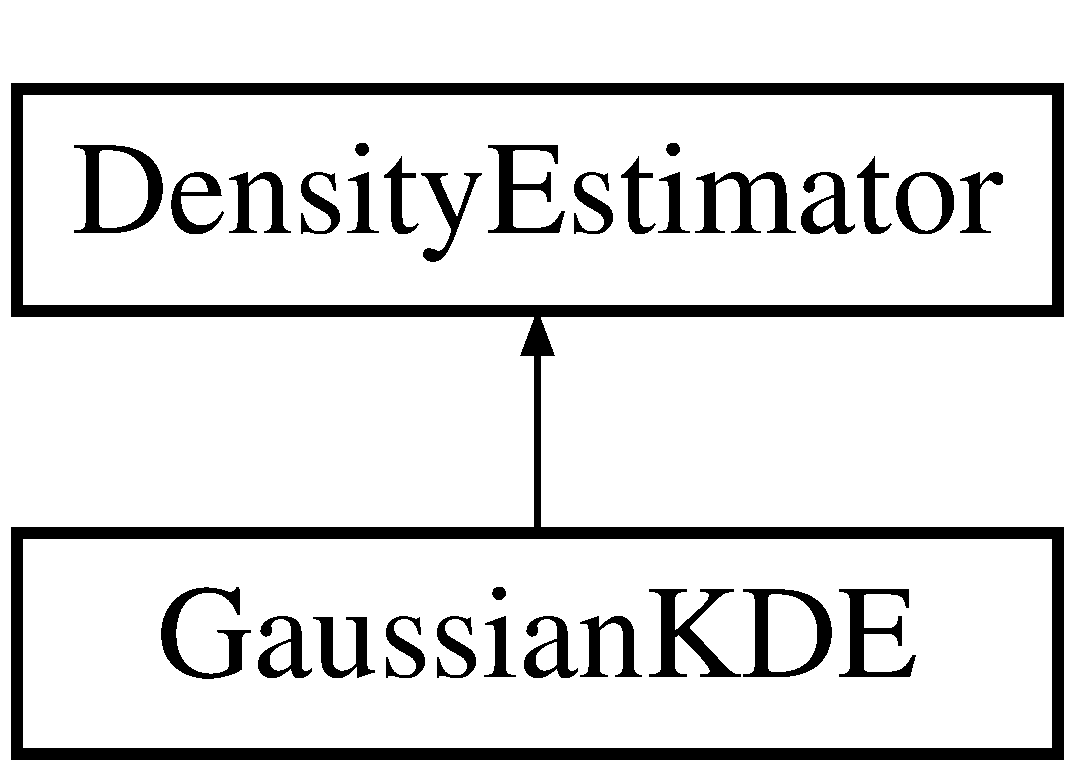
\includegraphics[height=2.000000cm]{classPecos_1_1DensityEstimator}
\end{center}
\end{figure}
\subsection*{Public Member Functions}
\begin{DoxyCompactItemize}
\item 
\hyperlink{classPecos_1_1DensityEstimator_a61d0043dfffa80f94cd77081f32be52d}{Density\+Estimator} ()
\begin{DoxyCompactList}\small\item\em default constructor \end{DoxyCompactList}\item 
\hyperlink{classPecos_1_1DensityEstimator_a0e6d09871df9b3ababad33371d95cefb}{Density\+Estimator} (const String \&density\+\_\+estimator\+\_\+type)
\begin{DoxyCompactList}\small\item\em standard constructor for envelope \end{DoxyCompactList}\item 
\hyperlink{classPecos_1_1DensityEstimator_acc375bcd034112a7c9b2e6b745ef8137}{Density\+Estimator} (const \hyperlink{classPecos_1_1DensityEstimator}{Density\+Estimator} \&density\+\_\+estimator)
\begin{DoxyCompactList}\small\item\em copy constructor \end{DoxyCompactList}\item 
virtual \hyperlink{classPecos_1_1DensityEstimator_a18e1bc50e0cf55f28ee89cd99a455798}{$\sim$\+Density\+Estimator} ()
\begin{DoxyCompactList}\small\item\em destructor \end{DoxyCompactList}\item 
\hyperlink{classPecos_1_1DensityEstimator}{Density\+Estimator} \hyperlink{classPecos_1_1DensityEstimator_a3f5714fb35670202d9f015a31a85138d}{operator=} (const \hyperlink{classPecos_1_1DensityEstimator}{Density\+Estimator} \&density\+\_\+estimator)
\begin{DoxyCompactList}\small\item\em assignment operator \end{DoxyCompactList}\item 
virtual void \hyperlink{classPecos_1_1DensityEstimator_a6c7e188a789efc33dbeb356f6e200c33}{initialize} (Real\+Matrix \&samples, Teuchos\+::\+E\+Transp trans=Teuchos\+::\+N\+O\+\_\+\+T\+R\+A\+NS)\label{classPecos_1_1DensityEstimator_a6c7e188a789efc33dbeb356f6e200c33}

\begin{DoxyCompactList}\small\item\em initialize the densities \end{DoxyCompactList}\item 
virtual void {\bfseries initialize} (Real\+Vector\+Array \&samples)\label{classPecos_1_1DensityEstimator_a50fd0e9c6addf748bf7ae040ec0d91f9}

\item 
virtual size\+\_\+t \hyperlink{classPecos_1_1DensityEstimator_a890ccac161f0becd266252b4cd3b9584}{get\+Dim} ()\label{classPecos_1_1DensityEstimator_a890ccac161f0becd266252b4cd3b9584}

\begin{DoxyCompactList}\small\item\em get the dimensionality \end{DoxyCompactList}\item 
virtual Real \hyperlink{classPecos_1_1DensityEstimator_adc6f262952d05a33ff68cae37929cbb2}{mean} ()\label{classPecos_1_1DensityEstimator_adc6f262952d05a33ff68cae37929cbb2}

\begin{DoxyCompactList}\small\item\em mean \end{DoxyCompactList}\item 
virtual Real \hyperlink{classPecos_1_1DensityEstimator_a38f6da77468be17e02ce38af2c0976c3}{variance} ()\label{classPecos_1_1DensityEstimator_a38f6da77468be17e02ce38af2c0976c3}

\begin{DoxyCompactList}\small\item\em variance \end{DoxyCompactList}\item 
virtual Real \hyperlink{classPecos_1_1DensityEstimator_a3e3c923ec6be63011f72bb65b08789ed}{std\+\_\+deviation} ()\label{classPecos_1_1DensityEstimator_a3e3c923ec6be63011f72bb65b08789ed}

\begin{DoxyCompactList}\small\item\em standard deviation \end{DoxyCompactList}\item 
virtual void \hyperlink{classPecos_1_1DensityEstimator_a8cf84ab65e0bccb16f5cdbccc9790dc9}{cov} (Real\+Matrix \&cov)\label{classPecos_1_1DensityEstimator_a8cf84ab65e0bccb16f5cdbccc9790dc9}

\begin{DoxyCompactList}\small\item\em computes the covariance matrix \end{DoxyCompactList}\item 
virtual void \hyperlink{classPecos_1_1DensityEstimator_a277fd59fe80b41f6ed6f5ff12e19f921}{corrcoeff} (Real\+Matrix \&corr)\label{classPecos_1_1DensityEstimator_a277fd59fe80b41f6ed6f5ff12e19f921}

\begin{DoxyCompactList}\small\item\em computes the correlation matrix \end{DoxyCompactList}\item 
virtual Real \hyperlink{classPecos_1_1DensityEstimator_ae49fd0166d0cedd899f933e3e2b713aa}{pdf} (const Real\+Vector \&x) const \label{classPecos_1_1DensityEstimator_ae49fd0166d0cedd899f933e3e2b713aa}

\begin{DoxyCompactList}\small\item\em operations for one sample \end{DoxyCompactList}\item 
virtual void \hyperlink{classPecos_1_1DensityEstimator_a83ef7a2b0cf786922fbdfb17d284d2e0}{pdf} (const Real\+Matrix \&data, Real\+Vector \&res, Teuchos\+::\+E\+Transp trans=Teuchos\+::\+N\+O\+\_\+\+T\+R\+A\+NS) const \label{classPecos_1_1DensityEstimator_a83ef7a2b0cf786922fbdfb17d284d2e0}

\begin{DoxyCompactList}\small\item\em operations for a set of samples \end{DoxyCompactList}\item 
virtual void \hyperlink{classPecos_1_1DensityEstimator_a5aa525959e7bee8034a26a77e00f12ef}{marginalize} (size\+\_\+t dim, \hyperlink{classPecos_1_1DensityEstimator}{Density\+Estimator} \&estimator)
\begin{DoxyCompactList}\small\item\em marginalization operations \end{DoxyCompactList}\item 
virtual void \hyperlink{classPecos_1_1DensityEstimator_a50f735eabae41f8948d792ac84749095}{marg\+To\+Dim\+Xs} (const Int\+Vector \&dims, \hyperlink{classPecos_1_1DensityEstimator}{Density\+Estimator} \&estimator)\label{classPecos_1_1DensityEstimator_a50f735eabae41f8948d792ac84749095}

\begin{DoxyCompactList}\small\item\em creates a maginalized density with remaining dims \end{DoxyCompactList}\item 
virtual void \hyperlink{classPecos_1_1DensityEstimator_ab1e735a6e2e62abfaa78e44d3a6bd9ec}{marg\+To\+DimX} (size\+\_\+t dim, \hyperlink{classPecos_1_1DensityEstimator}{Density\+Estimator} \&estimator)\label{classPecos_1_1DensityEstimator_ab1e735a6e2e62abfaa78e44d3a6bd9ec}

\begin{DoxyCompactList}\small\item\em creates a maginalized density with one remaining dimension \end{DoxyCompactList}\item 
virtual void \hyperlink{classPecos_1_1DensityEstimator_a48a43dfe8975d003c2c7cff695046414}{conditionalize} (const Real\+Vector \&x, const Int\+Vector \&dims, \hyperlink{classPecos_1_1DensityEstimator}{Density\+Estimator} \&estimator)\label{classPecos_1_1DensityEstimator_a48a43dfe8975d003c2c7cff695046414}

\begin{DoxyCompactList}\small\item\em conditionalization operations \end{DoxyCompactList}\item 
virtual void {\bfseries cond\+To\+DimX} (const Real\+Vector \&x, size\+\_\+t dim, \hyperlink{classPecos_1_1DensityEstimator}{Density\+Estimator} \&estimator)\label{classPecos_1_1DensityEstimator_aa4b4c620def1d4611d3e10dcd4b3a073}

\item 
String {\bfseries get\+Type} ()\label{classPecos_1_1DensityEstimator_a68adac94351807681f1b2828b9c68734}

\item 
\hyperlink{classPecos_1_1DensityEstimator}{Density\+Estimator} $\ast$ {\bfseries get\+Envelope} ()\label{classPecos_1_1DensityEstimator_a3b6f140849ddd8d260b08912f0ddde32}

\item 
bool {\bfseries is\+\_\+null} ()\label{classPecos_1_1DensityEstimator_a20a65eada5e4846ec27c12dd7166adec}

\end{DoxyCompactItemize}
\subsection*{Protected Attributes}
\begin{DoxyCompactItemize}
\item 
String {\bfseries density\+\_\+estimator\+\_\+type}\label{classPecos_1_1DensityEstimator_ab95f5d8568c1ff1e0a02a408fedb00eb}

\end{DoxyCompactItemize}
\subsection*{Static Private Member Functions}
\begin{DoxyCompactItemize}
\item 
static \hyperlink{classPecos_1_1DensityEstimator}{Density\+Estimator} $\ast$ \hyperlink{classPecos_1_1DensityEstimator_a531bb898be601c8a9e061574b536b1a4}{get\+\_\+density\+\_\+estimator} (const String \&density\+\_\+estimator\+\_\+type)
\end{DoxyCompactItemize}
\subsection*{Private Attributes}
\begin{DoxyCompactItemize}
\item 
\hyperlink{classPecos_1_1DensityEstimator}{Density\+Estimator} $\ast$ {\bfseries density\+Estimator}\label{classPecos_1_1DensityEstimator_ab9655a797c32d29656770a8044f38fff}

\item 
int \hyperlink{classPecos_1_1DensityEstimator_afff0b6144883d3ca09a8d0d3f4776b0f}{reference\+Count}\label{classPecos_1_1DensityEstimator_afff0b6144883d3ca09a8d0d3f4776b0f}

\begin{DoxyCompactList}\small\item\em number of objects sharing samples \end{DoxyCompactList}\end{DoxyCompactItemize}


\subsection{Detailed Description}
Base class for density estimation strategies. 

\subsection{Constructor \& Destructor Documentation}
\index{Pecos\+::\+Density\+Estimator@{Pecos\+::\+Density\+Estimator}!Density\+Estimator@{Density\+Estimator}}
\index{Density\+Estimator@{Density\+Estimator}!Pecos\+::\+Density\+Estimator@{Pecos\+::\+Density\+Estimator}}
\subsubsection[{\texorpdfstring{Density\+Estimator()}{DensityEstimator()}}]{\setlength{\rightskip}{0pt plus 5cm}{\bf Density\+Estimator} (
\begin{DoxyParamCaption}
{}
\end{DoxyParamCaption}
)}\label{classPecos_1_1DensityEstimator_a61d0043dfffa80f94cd77081f32be52d}


default constructor 

The default constructor\+: samples is N\+U\+LL in this case. This makes it necessary to check for N\+U\+LL in the copy constructor, assignment operator, and destructor. \index{Pecos\+::\+Density\+Estimator@{Pecos\+::\+Density\+Estimator}!Density\+Estimator@{Density\+Estimator}}
\index{Density\+Estimator@{Density\+Estimator}!Pecos\+::\+Density\+Estimator@{Pecos\+::\+Density\+Estimator}}
\subsubsection[{\texorpdfstring{Density\+Estimator(const String \&density\+\_\+estimator\+\_\+type)}{DensityEstimator(const String &density_estimator_type)}}]{\setlength{\rightskip}{0pt plus 5cm}{\bf Density\+Estimator} (
\begin{DoxyParamCaption}
\item[{const String \&}]{density\+\_\+estimator}
\end{DoxyParamCaption}
)}\label{classPecos_1_1DensityEstimator_a0e6d09871df9b3ababad33371d95cefb}


standard constructor for envelope 

Envelope constructor only needs to extract enough data to properly execute get\+\_\+density\+\_\+estimator, since Density\+Estimator(\+Base\+Constructor) builds the actual base class data for the derived transformations. 

References Density\+Estimator\+::get\+\_\+density\+\_\+estimator().

\index{Pecos\+::\+Density\+Estimator@{Pecos\+::\+Density\+Estimator}!Density\+Estimator@{Density\+Estimator}}
\index{Density\+Estimator@{Density\+Estimator}!Pecos\+::\+Density\+Estimator@{Pecos\+::\+Density\+Estimator}}
\subsubsection[{\texorpdfstring{Density\+Estimator(const Density\+Estimator \&density\+\_\+estimator)}{DensityEstimator(const DensityEstimator &density_estimator)}}]{\setlength{\rightskip}{0pt plus 5cm}{\bf Density\+Estimator} (
\begin{DoxyParamCaption}
\item[{const {\bf Density\+Estimator} \&}]{density\+\_\+estimator}
\end{DoxyParamCaption}
)}\label{classPecos_1_1DensityEstimator_acc375bcd034112a7c9b2e6b745ef8137}


copy constructor 

Copy constructor manages sharing of density\+Estimatorand incrementing of reference\+Count. 

References Density\+Estimator\+::reference\+Count.

\index{Pecos\+::\+Density\+Estimator@{Pecos\+::\+Density\+Estimator}!````~Density\+Estimator@{$\sim$\+Density\+Estimator}}
\index{````~Density\+Estimator@{$\sim$\+Density\+Estimator}!Pecos\+::\+Density\+Estimator@{Pecos\+::\+Density\+Estimator}}
\subsubsection[{\texorpdfstring{$\sim$\+Density\+Estimator()}{~DensityEstimator()}}]{\setlength{\rightskip}{0pt plus 5cm}$\sim${\bf Density\+Estimator} (
\begin{DoxyParamCaption}
{}
\end{DoxyParamCaption}
)\hspace{0.3cm}{\ttfamily [virtual]}}\label{classPecos_1_1DensityEstimator_a18e1bc50e0cf55f28ee89cd99a455798}


destructor 

Destructor decrements reference\+Count and only deletes data\+Trans\+Rep when reference\+Count reaches zero. 

References Density\+Estimator\+::reference\+Count.



\subsection{Member Function Documentation}
\index{Pecos\+::\+Density\+Estimator@{Pecos\+::\+Density\+Estimator}!operator=@{operator=}}
\index{operator=@{operator=}!Pecos\+::\+Density\+Estimator@{Pecos\+::\+Density\+Estimator}}
\subsubsection[{\texorpdfstring{operator=(const Density\+Estimator \&density\+\_\+estimator)}{operator=(const DensityEstimator &density_estimator)}}]{\setlength{\rightskip}{0pt plus 5cm}{\bf Density\+Estimator} operator= (
\begin{DoxyParamCaption}
\item[{const {\bf Density\+Estimator} \&}]{density\+\_\+estimator}
\end{DoxyParamCaption}
)}\label{classPecos_1_1DensityEstimator_a3f5714fb35670202d9f015a31a85138d}


assignment operator 

Assignment operator decrements reference\+Count for old data\+Trans\+Rep, assigns new data\+Trans\+Rep, and increments reference\+Count for new data\+Trans\+Rep. 

References Density\+Estimator\+::reference\+Count.

\index{Pecos\+::\+Density\+Estimator@{Pecos\+::\+Density\+Estimator}!marginalize@{marginalize}}
\index{marginalize@{marginalize}!Pecos\+::\+Density\+Estimator@{Pecos\+::\+Density\+Estimator}}
\subsubsection[{\texorpdfstring{marginalize(size\+\_\+t dim, Density\+Estimator \&estimator)}{marginalize(size_t dim, DensityEstimator &estimator)}}]{\setlength{\rightskip}{0pt plus 5cm}void marginalize (
\begin{DoxyParamCaption}
\item[{size\+\_\+t}]{dim, }
\item[{{\bf Density\+Estimator} \&}]{estimator}
\end{DoxyParamCaption}
)\hspace{0.3cm}{\ttfamily [virtual]}}\label{classPecos_1_1DensityEstimator_a5aa525959e7bee8034a26a77e00f12ef}


marginalization operations 

marginalizes over dim 

Reimplemented in \hyperlink{classPecos_1_1GaussianKDE_a5aa525959e7bee8034a26a77e00f12ef}{Gaussian\+K\+DE}.



References Density\+Estimator\+::marginalize().



Referenced by Density\+Estimator\+::marginalize().

\index{Pecos\+::\+Density\+Estimator@{Pecos\+::\+Density\+Estimator}!get\+\_\+density\+\_\+estimator@{get\+\_\+density\+\_\+estimator}}
\index{get\+\_\+density\+\_\+estimator@{get\+\_\+density\+\_\+estimator}!Pecos\+::\+Density\+Estimator@{Pecos\+::\+Density\+Estimator}}
\subsubsection[{\texorpdfstring{get\+\_\+density\+\_\+estimator(const String \&density\+\_\+estimator\+\_\+type)}{get_density_estimator(const String &density_estimator_type)}}]{\setlength{\rightskip}{0pt plus 5cm}{\bf Density\+Estimator} $\ast$ get\+\_\+density\+\_\+estimator (
\begin{DoxyParamCaption}
\item[{const String \&}]{density\+\_\+estimator\+\_\+type}
\end{DoxyParamCaption}
)\hspace{0.3cm}{\ttfamily [static]}, {\ttfamily [private]}}\label{classPecos_1_1DensityEstimator_a531bb898be601c8a9e061574b536b1a4}
Used only by the envelope constructor to initialize density\+Estimator to the appropriate derived type. 

Referenced by Density\+Estimator\+::\+Density\+Estimator().



The documentation for this class was generated from the following files\+:\begin{DoxyCompactItemize}
\item 
Density\+Estimator.\+hpp\item 
Density\+Estimator.\+cpp\end{DoxyCompactItemize}

\section{Epistemic\+Dist\+Params Class Reference}
\label{classPecos_1_1EpistemicDistParams}\index{Epistemic\+Dist\+Params@{Epistemic\+Dist\+Params}}


Container class encapsulating distribution parameters for epistemic random variables.  


\subsection*{Public Member Functions}
\begin{DoxyCompactItemize}
\item 
\hyperlink{classPecos_1_1EpistemicDistParams_a5c947f7c65c8d4bd42e89d30c21d0ee5}{Epistemic\+Dist\+Params} ()\label{classPecos_1_1EpistemicDistParams_a5c947f7c65c8d4bd42e89d30c21d0ee5}

\begin{DoxyCompactList}\small\item\em default constructor \end{DoxyCompactList}\item 
\hyperlink{classPecos_1_1EpistemicDistParams_a80c694a3f408daeb46249fea90258381}{Epistemic\+Dist\+Params} (const Real\+Real\+Pair\+Real\+Map\+Array \&ceuv\+\_\+bpas, const Int\+Int\+Pair\+Real\+Map\+Array \&deuiv\+\_\+bpas, const Int\+Real\+Map\+Array \&deusiv\+\_\+vals\+\_\+probs, const String\+Real\+Map\+Array \&deussv\+\_\+vals\+\_\+probs, const Real\+Real\+Map\+Array \&deusrv\+\_\+vals\+\_\+probs)\label{classPecos_1_1EpistemicDistParams_a80c694a3f408daeb46249fea90258381}

\begin{DoxyCompactList}\small\item\em standard constructor \end{DoxyCompactList}\item 
\hyperlink{classPecos_1_1EpistemicDistParams_a51140bd8c73fc26045fef144d105f03c}{Epistemic\+Dist\+Params} (const \hyperlink{classPecos_1_1EpistemicDistParams}{Epistemic\+Dist\+Params} \&edp)\label{classPecos_1_1EpistemicDistParams_a51140bd8c73fc26045fef144d105f03c}

\begin{DoxyCompactList}\small\item\em copy constructor \end{DoxyCompactList}\item 
\hyperlink{classPecos_1_1EpistemicDistParams_a78317b2e084d2b5f6393353706674649}{$\sim$\+Epistemic\+Dist\+Params} ()\label{classPecos_1_1EpistemicDistParams_a78317b2e084d2b5f6393353706674649}

\begin{DoxyCompactList}\small\item\em destructor \end{DoxyCompactList}\item 
\hyperlink{classPecos_1_1EpistemicDistParams}{Epistemic\+Dist\+Params} \& \hyperlink{classPecos_1_1EpistemicDistParams_a27a62dcc32abd4faea77c62e9f0e7e73}{operator=} (const \hyperlink{classPecos_1_1EpistemicDistParams}{Epistemic\+Dist\+Params} \&edp)\label{classPecos_1_1EpistemicDistParams_a27a62dcc32abd4faea77c62e9f0e7e73}

\begin{DoxyCompactList}\small\item\em assignment operator \end{DoxyCompactList}\item 
size\+\_\+t \hyperlink{classPecos_1_1EpistemicDistParams_a4c50fa5198ce132eb8339e1736012949}{ceuv} () const \label{classPecos_1_1EpistemicDistParams_a4c50fa5198ce132eb8339e1736012949}

\begin{DoxyCompactList}\small\item\em return total number of continuous epistemic uncertain variables \end{DoxyCompactList}\item 
size\+\_\+t \hyperlink{classPecos_1_1EpistemicDistParams_a8368a575e55d7fc0380aa9771c1201bc}{deuiv} () const \label{classPecos_1_1EpistemicDistParams_a8368a575e55d7fc0380aa9771c1201bc}

\begin{DoxyCompactList}\small\item\em return total number of discrete epistemic uncertain integer variables \end{DoxyCompactList}\item 
size\+\_\+t \hyperlink{classPecos_1_1EpistemicDistParams_a8b1da44c48aeed96bc9b5e3d1dbb772c}{deusv} () const \label{classPecos_1_1EpistemicDistParams_a8b1da44c48aeed96bc9b5e3d1dbb772c}

\begin{DoxyCompactList}\small\item\em return total number of discrete epistemic uncertain string variables \end{DoxyCompactList}\item 
size\+\_\+t \hyperlink{classPecos_1_1EpistemicDistParams_a4c63a27e1f93b03574f04b4c8ae57bf1}{deurv} () const \label{classPecos_1_1EpistemicDistParams_a4c63a27e1f93b03574f04b4c8ae57bf1}

\begin{DoxyCompactList}\small\item\em return total number of discrete epistemic uncertain real variables \end{DoxyCompactList}\item 
size\+\_\+t \hyperlink{classPecos_1_1EpistemicDistParams_a3b5119d9164fd536a51500137c3522ca}{deuv} () const \label{classPecos_1_1EpistemicDistParams_a3b5119d9164fd536a51500137c3522ca}

\begin{DoxyCompactList}\small\item\em return total number of discrete epistemic uncertain variables \end{DoxyCompactList}\item 
void \hyperlink{classPecos_1_1EpistemicDistParams_ac07244686fa7a745617167aaae7dc2f1}{copy} (const \hyperlink{classPecos_1_1EpistemicDistParams}{Epistemic\+Dist\+Params} \&edp)\label{classPecos_1_1EpistemicDistParams_ac07244686fa7a745617167aaae7dc2f1}

\begin{DoxyCompactList}\small\item\em deep copy (as opposed to operator= shallow copy) \end{DoxyCompactList}\item 
void \hyperlink{classPecos_1_1EpistemicDistParams_a46786dc519d291b28119cd39fa5f47be}{update} (const \hyperlink{classPecos_1_1EpistemicDistParams}{Epistemic\+Dist\+Params} \&edp)\label{classPecos_1_1EpistemicDistParams_a46786dc519d291b28119cd39fa5f47be}

\begin{DoxyCompactList}\small\item\em data update (no changes to representation (unless null)) \end{DoxyCompactList}\item 
const Real\+Real\+Pair\+Real\+Map\+Array \& \hyperlink{classPecos_1_1EpistemicDistParams_adf39419d5f98afe9ade91fb12f504e70}{continuous\+\_\+interval\+\_\+basic\+\_\+probabilities} () const \label{classPecos_1_1EpistemicDistParams_adf39419d5f98afe9ade91fb12f504e70}

\begin{DoxyCompactList}\small\item\em return the interval basic probability values \end{DoxyCompactList}\item 
const Real\+Real\+Pair\+Real\+Map \& \hyperlink{classPecos_1_1EpistemicDistParams_ab09bde881523a715cf5fb5afe50f70d7}{continuous\+\_\+interval\+\_\+basic\+\_\+probabilities} (size\+\_\+t i) const \label{classPecos_1_1EpistemicDistParams_ab09bde881523a715cf5fb5afe50f70d7}

\begin{DoxyCompactList}\small\item\em return the ith interval basic probability value \end{DoxyCompactList}\item 
void \hyperlink{classPecos_1_1EpistemicDistParams_a2c3625cd2630f60190f07b53785c8cc5}{continuous\+\_\+interval\+\_\+basic\+\_\+probabilities} (const Real\+Real\+Pair\+Real\+Map\+Array \&ci\+\_\+probs)\label{classPecos_1_1EpistemicDistParams_a2c3625cd2630f60190f07b53785c8cc5}

\begin{DoxyCompactList}\small\item\em set the interval basic probability values \end{DoxyCompactList}\item 
void \hyperlink{classPecos_1_1EpistemicDistParams_a1da79481eb1ec165f57b05f5dd50717e}{continuous\+\_\+interval\+\_\+basic\+\_\+probabilities} (const Real\+Real\+Pair\+Real\+Map \&ci\+\_\+probs\+\_\+i, size\+\_\+t i)\label{classPecos_1_1EpistemicDistParams_a1da79481eb1ec165f57b05f5dd50717e}

\begin{DoxyCompactList}\small\item\em set the ith interval basic probability value \end{DoxyCompactList}\item 
const Int\+Int\+Pair\+Real\+Map\+Array \& \hyperlink{classPecos_1_1EpistemicDistParams_a5aa40a7ca7bb934dcf571f3689c4e1ae}{discrete\+\_\+interval\+\_\+basic\+\_\+probabilities} () const \label{classPecos_1_1EpistemicDistParams_a5aa40a7ca7bb934dcf571f3689c4e1ae}

\begin{DoxyCompactList}\small\item\em return the interval basic probability values \end{DoxyCompactList}\item 
const Int\+Int\+Pair\+Real\+Map \& \hyperlink{classPecos_1_1EpistemicDistParams_a2dc76c64e24f6f7dd04eef06ed924243}{discrete\+\_\+interval\+\_\+basic\+\_\+probabilities} (size\+\_\+t i) const \label{classPecos_1_1EpistemicDistParams_a2dc76c64e24f6f7dd04eef06ed924243}

\begin{DoxyCompactList}\small\item\em return the ith interval basic probability value \end{DoxyCompactList}\item 
void \hyperlink{classPecos_1_1EpistemicDistParams_a915b0bd8df63bcbb0de82d1cf19c1a36}{discrete\+\_\+interval\+\_\+basic\+\_\+probabilities} (const Int\+Int\+Pair\+Real\+Map\+Array \&di\+\_\+bpa)\label{classPecos_1_1EpistemicDistParams_a915b0bd8df63bcbb0de82d1cf19c1a36}

\begin{DoxyCompactList}\small\item\em set the interval basic probability values \end{DoxyCompactList}\item 
void \hyperlink{classPecos_1_1EpistemicDistParams_a7406fef4e867900f229ff6620a7db85b}{discrete\+\_\+interval\+\_\+basic\+\_\+probabilities} (const Int\+Int\+Pair\+Real\+Map \&di\+\_\+bpa\+\_\+i, size\+\_\+t i)\label{classPecos_1_1EpistemicDistParams_a7406fef4e867900f229ff6620a7db85b}

\begin{DoxyCompactList}\small\item\em set the ith interval basic probability value \end{DoxyCompactList}\item 
const Int\+Real\+Map\+Array \& \hyperlink{classPecos_1_1EpistemicDistParams_a74664dadc4c09d0f154e6ecc7db882cf}{discrete\+\_\+set\+\_\+int\+\_\+values\+\_\+probabilities} () const \label{classPecos_1_1EpistemicDistParams_a74664dadc4c09d0f154e6ecc7db882cf}

\begin{DoxyCompactList}\small\item\em get the discrete integer set values and probabilities \end{DoxyCompactList}\item 
void \hyperlink{classPecos_1_1EpistemicDistParams_a643ede8b8b26ba40b3940ee4cb3843ac}{discrete\+\_\+set\+\_\+int\+\_\+values\+\_\+probabilities} (const Int\+Real\+Map\+Array \&dsi\+\_\+vals\+\_\+probs)\label{classPecos_1_1EpistemicDistParams_a643ede8b8b26ba40b3940ee4cb3843ac}

\begin{DoxyCompactList}\small\item\em set the discrete integer set values and probabilities \end{DoxyCompactList}\item 
const String\+Real\+Map\+Array \& \hyperlink{classPecos_1_1EpistemicDistParams_a8dd6ed1e2754ce0bec6eb0c804b0f015}{discrete\+\_\+set\+\_\+string\+\_\+values\+\_\+probabilities} () const \label{classPecos_1_1EpistemicDistParams_a8dd6ed1e2754ce0bec6eb0c804b0f015}

\begin{DoxyCompactList}\small\item\em get the discrete string set values and probabilities \end{DoxyCompactList}\item 
void \hyperlink{classPecos_1_1EpistemicDistParams_aaf98a6c246d0872e1dc08a56c4d844b7}{discrete\+\_\+set\+\_\+string\+\_\+values\+\_\+probabilities} (const String\+Real\+Map\+Array \&dss\+\_\+vals\+\_\+probs)\label{classPecos_1_1EpistemicDistParams_aaf98a6c246d0872e1dc08a56c4d844b7}

\begin{DoxyCompactList}\small\item\em set the discrete string set values and probabilities \end{DoxyCompactList}\item 
const Real\+Real\+Map\+Array \& \hyperlink{classPecos_1_1EpistemicDistParams_a301a5cf39eb4819c0bc02ae9611816fc}{discrete\+\_\+set\+\_\+real\+\_\+values\+\_\+probabilities} () const \label{classPecos_1_1EpistemicDistParams_a301a5cf39eb4819c0bc02ae9611816fc}

\begin{DoxyCompactList}\small\item\em get the discrete real set values and probabilities \end{DoxyCompactList}\item 
void \hyperlink{classPecos_1_1EpistemicDistParams_a5f30869a14a22a36696c6ea5533988ef}{discrete\+\_\+set\+\_\+real\+\_\+values\+\_\+probabilities} (const Real\+Real\+Map\+Array \&dsr\+\_\+vals\+\_\+probs)\label{classPecos_1_1EpistemicDistParams_a5f30869a14a22a36696c6ea5533988ef}

\begin{DoxyCompactList}\small\item\em set the discrete real set values and probabilities \end{DoxyCompactList}\item 
bool \hyperlink{classPecos_1_1EpistemicDistParams_a3c45461717ff230edd665ce24da988c5}{is\+\_\+null} () const \label{classPecos_1_1EpistemicDistParams_a3c45461717ff230edd665ce24da988c5}

\begin{DoxyCompactList}\small\item\em function to check edp\+Rep (does this handle contain a body) \end{DoxyCompactList}\end{DoxyCompactItemize}
\subsection*{Private Attributes}
\begin{DoxyCompactItemize}
\item 
\hyperlink{classPecos_1_1EpistemicDistParamsRep}{Epistemic\+Dist\+Params\+Rep} $\ast$ \hyperlink{classPecos_1_1EpistemicDistParams_a71048d7ae6a93a250f1ba1935a5d002c}{edp\+Rep}\label{classPecos_1_1EpistemicDistParams_a71048d7ae6a93a250f1ba1935a5d002c}

\begin{DoxyCompactList}\small\item\em pointer to the body (handle-\/body idiom) \end{DoxyCompactList}\end{DoxyCompactItemize}


\subsection{Detailed Description}
Container class encapsulating distribution parameters for epistemic random variables. 

This class consolidates epistemic distribution data and simplifies the A\+P\+Is that require distribution parameters. 

The documentation for this class was generated from the following file\+:\begin{DoxyCompactItemize}
\item 
Distribution\+Params.\+hpp\end{DoxyCompactItemize}

\section{Epistemic\+Dist\+Params\+Rep Class Reference}
\label{classPecos_1_1EpistemicDistParamsRep}\index{Epistemic\+Dist\+Params\+Rep@{Epistemic\+Dist\+Params\+Rep}}


The representation of a set of epistemic distribution parameters. This representation, or body, may be shared by multiple \hyperlink{classPecos_1_1EpistemicDistParams}{Epistemic\+Dist\+Params} handle instances.  


\subsection*{Private Member Functions}
\begin{DoxyCompactItemize}
\item 
\hyperlink{classPecos_1_1EpistemicDistParamsRep_aa0540ab459e27f052ac00aaa0b8d45c7}{Epistemic\+Dist\+Params\+Rep} ()\label{classPecos_1_1EpistemicDistParamsRep_aa0540ab459e27f052ac00aaa0b8d45c7}

\begin{DoxyCompactList}\small\item\em default constructor \end{DoxyCompactList}\item 
\hyperlink{classPecos_1_1EpistemicDistParamsRep_acb29b99dae9cfb57eba028d27a7de0ab}{Epistemic\+Dist\+Params\+Rep} (const Real\+Real\+Pair\+Real\+Map\+Array \&ceuv\+\_\+bpas, const Int\+Int\+Pair\+Real\+Map\+Array \&deuiv\+\_\+bpas, const Int\+Real\+Map\+Array \&deusiv\+\_\+vals\+\_\+probs, const String\+Real\+Map\+Array \&deussv\+\_\+vals\+\_\+probs, const Real\+Real\+Map\+Array \&deusrv\+\_\+vals\+\_\+probs)\label{classPecos_1_1EpistemicDistParamsRep_acb29b99dae9cfb57eba028d27a7de0ab}

\begin{DoxyCompactList}\small\item\em constructor \end{DoxyCompactList}\item 
\hyperlink{classPecos_1_1EpistemicDistParamsRep_a69939dd1df7f5cf6dc996f723026ac99}{$\sim$\+Epistemic\+Dist\+Params\+Rep} ()\label{classPecos_1_1EpistemicDistParamsRep_a69939dd1df7f5cf6dc996f723026ac99}

\begin{DoxyCompactList}\small\item\em destructor \end{DoxyCompactList}\end{DoxyCompactItemize}
\subsection*{Private Attributes}
\begin{DoxyCompactItemize}
\item 
Real\+Real\+Pair\+Real\+Map\+Array \hyperlink{classPecos_1_1EpistemicDistParamsRep_a9eaf4bb36ecab2682ba05d44b6619f14}{cont\+Interval\+B\+PA}\label{classPecos_1_1EpistemicDistParamsRep_a9eaf4bb36ecab2682ba05d44b6619f14}

\begin{DoxyCompactList}\small\item\em basic probability assignments (continuous interval bounds + probability) for continuous interval uncertain variables \end{DoxyCompactList}\item 
Int\+Int\+Pair\+Real\+Map\+Array \hyperlink{classPecos_1_1EpistemicDistParamsRep_a1f3f8a098c4bb51d2920395c0e29b7aa}{disc\+Interval\+B\+PA}\label{classPecos_1_1EpistemicDistParamsRep_a1f3f8a098c4bb51d2920395c0e29b7aa}

\begin{DoxyCompactList}\small\item\em basic probability assignments (discrete range bounds + probability) for discrete interval uncertain variables \end{DoxyCompactList}\item 
Int\+Real\+Map\+Array \hyperlink{classPecos_1_1EpistemicDistParamsRep_a60e7f972e185361ba1ca7bd9feff219f}{disc\+Set\+Int\+Vals\+Probs}\label{classPecos_1_1EpistemicDistParamsRep_a60e7f972e185361ba1ca7bd9feff219f}

\begin{DoxyCompactList}\small\item\em admissible values and basic probability assignments for discrete uncertain set integer variables \end{DoxyCompactList}\item 
String\+Real\+Map\+Array \hyperlink{classPecos_1_1EpistemicDistParamsRep_aa46741d9f0a8f10cc40138ebaefdb834}{disc\+Set\+String\+Vals\+Probs}\label{classPecos_1_1EpistemicDistParamsRep_aa46741d9f0a8f10cc40138ebaefdb834}

\begin{DoxyCompactList}\small\item\em admissible values and basic probability assignments for discrete uncertain set string variables \end{DoxyCompactList}\item 
Real\+Real\+Map\+Array \hyperlink{classPecos_1_1EpistemicDistParamsRep_aaf3880a0b86a8f541bb48793662785e8}{disc\+Set\+Real\+Vals\+Probs}\label{classPecos_1_1EpistemicDistParamsRep_aaf3880a0b86a8f541bb48793662785e8}

\begin{DoxyCompactList}\small\item\em admissible values and basic probability assignments for discrete uncertain set real variables \end{DoxyCompactList}\item 
int \hyperlink{classPecos_1_1EpistemicDistParamsRep_afff0b6144883d3ca09a8d0d3f4776b0f}{reference\+Count}\label{classPecos_1_1EpistemicDistParamsRep_afff0b6144883d3ca09a8d0d3f4776b0f}

\begin{DoxyCompactList}\small\item\em number of handle objects sharing edp\+Rep \end{DoxyCompactList}\end{DoxyCompactItemize}
\subsection*{Friends}
\begin{DoxyCompactItemize}
\item 
class \hyperlink{classPecos_1_1EpistemicDistParamsRep_a2a3370b29dbf1ac16f49b525603d2e96}{Epistemic\+Dist\+Params}\label{classPecos_1_1EpistemicDistParamsRep_a2a3370b29dbf1ac16f49b525603d2e96}

\begin{DoxyCompactList}\small\item\em the handle class can access attributes of the body class directly \end{DoxyCompactList}\end{DoxyCompactItemize}


\subsection{Detailed Description}
The representation of a set of epistemic distribution parameters. This representation, or body, may be shared by multiple \hyperlink{classPecos_1_1EpistemicDistParams}{Epistemic\+Dist\+Params} handle instances. 

The Epistemic\+Dist\+Params/\+Epistemic\+Dist\+Params\+Rep pairs utilize a handle-\/body idiom (Coplien, Advanced C++). 

The documentation for this class was generated from the following file\+:\begin{DoxyCompactItemize}
\item 
Distribution\+Params.\+hpp\end{DoxyCompactItemize}

\section{Expansion\+Config\+Options Class Reference}
\label{classPecos_1_1ExpansionConfigOptions}\index{Expansion\+Config\+Options@{Expansion\+Config\+Options}}


Container class for various expansion configuration options.  


\subsection*{Public Member Functions}
\begin{DoxyCompactItemize}
\item 
\hyperlink{classPecos_1_1ExpansionConfigOptions_a0f799f4b0d6b136850a3f8dcffa92d0e}{Expansion\+Config\+Options} ()\label{classPecos_1_1ExpansionConfigOptions_a0f799f4b0d6b136850a3f8dcffa92d0e}

\begin{DoxyCompactList}\small\item\em default constructor \end{DoxyCompactList}\item 
\hyperlink{classPecos_1_1ExpansionConfigOptions_af12f42d383b2952656d1738710545660}{Expansion\+Config\+Options} (short exp\+\_\+soln\+\_\+approach, short exp\+\_\+basis\+\_\+type, short combine\+\_\+type, short discrep\+\_\+type, short output\+\_\+level, bool vbd\+\_\+flag, unsigned short vbd\+\_\+order, short refine\+\_\+cntl, int max\+\_\+refine\+\_\+iter, int max\+\_\+solver\+\_\+iter, Real conv\+\_\+tol, unsigned short sc\+\_\+limit)\label{classPecos_1_1ExpansionConfigOptions_af12f42d383b2952656d1738710545660}

\begin{DoxyCompactList}\small\item\em constructor \end{DoxyCompactList}\item 
\hyperlink{classPecos_1_1ExpansionConfigOptions_af383162dc15e844eceeb8d8839a80f76}{Expansion\+Config\+Options} (const \hyperlink{classPecos_1_1ExpansionConfigOptions}{Expansion\+Config\+Options} \&ec\+\_\+options)\label{classPecos_1_1ExpansionConfigOptions_af383162dc15e844eceeb8d8839a80f76}

\begin{DoxyCompactList}\small\item\em copy constructor \end{DoxyCompactList}\item 
\hyperlink{classPecos_1_1ExpansionConfigOptions_adcd10ff74da8317dd2f68fd4dc7a8980}{$\sim$\+Expansion\+Config\+Options} ()\label{classPecos_1_1ExpansionConfigOptions_adcd10ff74da8317dd2f68fd4dc7a8980}

\begin{DoxyCompactList}\small\item\em destructor \end{DoxyCompactList}\end{DoxyCompactItemize}
\subsection*{Public Attributes}
\begin{DoxyCompactItemize}
\item 
short \hyperlink{classPecos_1_1ExpansionConfigOptions_aab384268a7f9d05bb3a53de1dfcf9244}{exp\+Coeffs\+Soln\+Approach}\label{classPecos_1_1ExpansionConfigOptions_aab384268a7f9d05bb3a53de1dfcf9244}

\begin{DoxyCompactList}\small\item\em identifies the approach taken in compute\+\_\+coefficients()\+: Q\+U\+A\+D\+R\+A\+T\+U\+RE, C\+U\+B\+A\+T\+U\+RE, C\+O\+M\+B\+I\+N\+E\+D\+\_\+\+S\+P\+A\+R\+S\+E\+\_\+\+G\+R\+ID, H\+I\+E\+R\+A\+R\+C\+H\+I\+C\+A\+L\+\_\+\+S\+P\+A\+R\+S\+E\+\_\+\+G\+R\+ID, R\+E\+G\+R\+E\+S\+S\+I\+ON, or S\+A\+M\+P\+L\+I\+NG \end{DoxyCompactList}\item 
short \hyperlink{classPecos_1_1ExpansionConfigOptions_a4df6d933ebf73fcf30f55b8cdb5d2b11}{exp\+Basis\+Type}\label{classPecos_1_1ExpansionConfigOptions_a4df6d933ebf73fcf30f55b8cdb5d2b11}

\begin{DoxyCompactList}\small\item\em identifies the type of basis for the expansion\+: D\+E\+F\+A\+U\+L\+T\+\_\+\+B\+A\+S\+IS or \{N\+O\+D\+AL,H\+I\+E\+R\+A\+R\+C\+H\+I\+C\+AL\}\+\_\+\+I\+N\+T\+E\+R\+P\+O\+L\+A\+NT for SC or \{T\+E\+N\+S\+O\+R\+\_\+\+P\+R\+O\+D\+U\+CT,T\+O\+T\+A\+L\+\_\+\+O\+R\+D\+ER,A\+D\+A\+P\+T\+ED\}\+\_\+\+B\+A\+S\+IS for P\+CE regression \end{DoxyCompactList}\item 
short \hyperlink{classPecos_1_1ExpansionConfigOptions_a5f00b865c145833acbf962bab708af39}{combine\+Type}\label{classPecos_1_1ExpansionConfigOptions_a5f00b865c145833acbf962bab708af39}

\begin{DoxyCompactList}\small\item\em type of expansion combination\+: additive, multiplicative, or both \end{DoxyCompactList}\item 
short \hyperlink{classPecos_1_1ExpansionConfigOptions_acba8ffe2ebba12eb6492cea029cc9bf0}{discrepancy\+Type}\label{classPecos_1_1ExpansionConfigOptions_acba8ffe2ebba12eb6492cea029cc9bf0}

\begin{DoxyCompactList}\small\item\em type of multilevel discrepancy emulation\+: distinct or recursive \end{DoxyCompactList}\item 
short \hyperlink{classPecos_1_1ExpansionConfigOptions_a8b080aab3a786ee1439b43c3533f1f6a}{output\+Level}\label{classPecos_1_1ExpansionConfigOptions_a8b080aab3a786ee1439b43c3533f1f6a}

\begin{DoxyCompactList}\small\item\em output verbosity level\+: \{S\+I\+L\+E\+NT,Q\+U\+I\+ET,N\+O\+R\+M\+AL,V\+E\+R\+B\+O\+SE,D\+E\+B\+UG\}\+\_\+\+O\+U\+T\+P\+UT \end{DoxyCompactList}\item 
bool \hyperlink{classPecos_1_1ExpansionConfigOptions_a7245a7ac6fed7086737a74de2d14e351}{vbd\+Flag}\label{classPecos_1_1ExpansionConfigOptions_a7245a7ac6fed7086737a74de2d14e351}

\begin{DoxyCompactList}\small\item\em flag indicated use of variance-\/based decomposition for computing Sobol\textquotesingle{} indices \end{DoxyCompactList}\item 
unsigned short \hyperlink{classPecos_1_1ExpansionConfigOptions_afc2fc7de610d61c8b26d7a539175e140}{vbd\+Order\+Limit}\label{classPecos_1_1ExpansionConfigOptions_afc2fc7de610d61c8b26d7a539175e140}

\begin{DoxyCompactList}\small\item\em limit for order of interactions computed in variance-\/based decomposition \end{DoxyCompactList}\item 
short \hyperlink{classPecos_1_1ExpansionConfigOptions_a220ded02774967c0e361d4f6707c47a1}{refinement\+Control}\label{classPecos_1_1ExpansionConfigOptions_a220ded02774967c0e361d4f6707c47a1}

\begin{DoxyCompactList}\small\item\em approach for control of refinement\+: \{NO,U\+N\+I\+F\+O\+RM,L\+O\+C\+A\+L\+\_\+\+A\+D\+A\+P\+T\+I\+VE\}\+\_\+\+C\+O\+N\+T\+R\+OL or D\+I\+M\+E\+N\+S\+I\+O\+N\+\_\+\+A\+D\+A\+P\+T\+I\+V\+E\+\_\+\+C\+O\+N\+T\+R\+O\+L\+\_\+\{S\+O\+B\+OL,D\+E\+C\+AY,G\+E\+N\+E\+R\+A\+L\+I\+Z\+ED\} \end{DoxyCompactList}\item 
int \hyperlink{classPecos_1_1ExpansionConfigOptions_a55b1d40dab6511038dfd557e0c4feb31}{max\+Refine\+Iterations}\label{classPecos_1_1ExpansionConfigOptions_a55b1d40dab6511038dfd557e0c4feb31}

\begin{DoxyCompactList}\small\item\em control for limiting the maximum number of refinement iterations in adapted approximation algorithms \end{DoxyCompactList}\item 
int \hyperlink{classPecos_1_1ExpansionConfigOptions_a8ed5aaf09f80b5da21ec21fda71eb25f}{max\+Solver\+Iterations}\label{classPecos_1_1ExpansionConfigOptions_a8ed5aaf09f80b5da21ec21fda71eb25f}

\begin{DoxyCompactList}\small\item\em control for limiting the maximum number of solver iterations in iterative solver-\/based approximation algorithms (e.\+g., regularized regression) \end{DoxyCompactList}\item 
Real \hyperlink{classPecos_1_1ExpansionConfigOptions_adfa55b33af02e0710cef939a4b49c498}{convergence\+Tol}\label{classPecos_1_1ExpansionConfigOptions_adfa55b33af02e0710cef939a4b49c498}

\begin{DoxyCompactList}\small\item\em convergence tolerance for adapted or iterated approximation algorithms \end{DoxyCompactList}\item 
unsigned short \hyperlink{classPecos_1_1ExpansionConfigOptions_aa5315f8c8b2844fb38b15f8a8884a34d}{soft\+Conv\+Limit}\label{classPecos_1_1ExpansionConfigOptions_aa5315f8c8b2844fb38b15f8a8884a34d}

\begin{DoxyCompactList}\small\item\em number of consecutive cycles for which convergence criterion must be met prior to termination \end{DoxyCompactList}\end{DoxyCompactItemize}


\subsection{Detailed Description}
Container class for various expansion configuration options. 

The \hyperlink{classPecos_1_1ExpansionConfigOptions}{Expansion\+Config\+Options} class provides a simple container class for expansion configuration options related to data modes, verbosity, refinement, and V\+BD controls. 

The documentation for this class was generated from the following file\+:\begin{DoxyCompactItemize}
\item 
Shared\+Poly\+Approx\+Data.\+hpp\end{DoxyCompactItemize}

\section{Exponential\+Random\+Variable Class Reference}
\label{classPecos_1_1ExponentialRandomVariable}\index{Exponential\+Random\+Variable@{Exponential\+Random\+Variable}}


Derived random variable class for exponential random variables.  


Inheritance diagram for Exponential\+Random\+Variable\+:\begin{figure}[H]
\begin{center}
\leavevmode
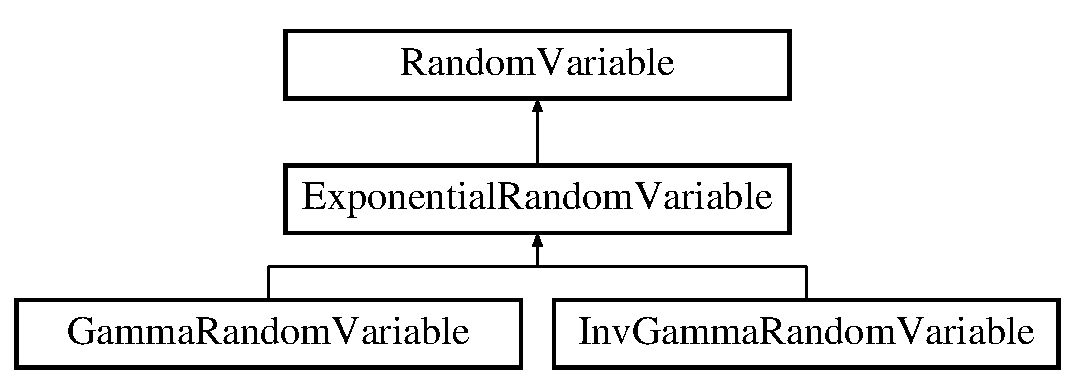
\includegraphics[height=3.000000cm]{classPecos_1_1ExponentialRandomVariable}
\end{center}
\end{figure}
\subsection*{Public Member Functions}
\begin{DoxyCompactItemize}
\item 
\hyperlink{classPecos_1_1ExponentialRandomVariable_a649f7f5eda7937ba25ae93c6a49c39c2}{Exponential\+Random\+Variable} ()\label{classPecos_1_1ExponentialRandomVariable_a649f7f5eda7937ba25ae93c6a49c39c2}

\begin{DoxyCompactList}\small\item\em default constructor \end{DoxyCompactList}\item 
\hyperlink{classPecos_1_1ExponentialRandomVariable_a9666904f0a8ac0f1b154bd6a840e3b49}{Exponential\+Random\+Variable} (Real beta)\label{classPecos_1_1ExponentialRandomVariable_a9666904f0a8ac0f1b154bd6a840e3b49}

\begin{DoxyCompactList}\small\item\em alternate constructor \end{DoxyCompactList}\item 
\hyperlink{classPecos_1_1ExponentialRandomVariable_ae1786ff9437473f381ece94d313975b2}{$\sim$\+Exponential\+Random\+Variable} ()\label{classPecos_1_1ExponentialRandomVariable_ae1786ff9437473f381ece94d313975b2}

\begin{DoxyCompactList}\small\item\em destructor \end{DoxyCompactList}\item 
Real \hyperlink{classPecos_1_1ExponentialRandomVariable_addd564e7f4f314e12d38df74d845f0d8}{cdf} (Real x) const \label{classPecos_1_1ExponentialRandomVariable_addd564e7f4f314e12d38df74d845f0d8}

\begin{DoxyCompactList}\small\item\em return the cumulative distribution function value of the random variable at x \end{DoxyCompactList}\item 
Real \hyperlink{classPecos_1_1ExponentialRandomVariable_a23c3b599e7e4788a9a5e9e93c3dbaf4d}{ccdf} (Real x) const \label{classPecos_1_1ExponentialRandomVariable_a23c3b599e7e4788a9a5e9e93c3dbaf4d}

\begin{DoxyCompactList}\small\item\em return the complementary cumulative distribution function value of the random variable at x \end{DoxyCompactList}\item 
Real \hyperlink{classPecos_1_1ExponentialRandomVariable_a918a1aac05ca349ea5313eebcba46c3e}{inverse\+\_\+cdf} (Real p\+\_\+cdf) const \label{classPecos_1_1ExponentialRandomVariable_a918a1aac05ca349ea5313eebcba46c3e}

\begin{DoxyCompactList}\small\item\em return the x value corresponding to a cumulative probability \end{DoxyCompactList}\item 
Real \hyperlink{classPecos_1_1ExponentialRandomVariable_afda003a1f59ff6930902cd5c8601f49b}{inverse\+\_\+ccdf} (Real p\+\_\+ccdf) const \label{classPecos_1_1ExponentialRandomVariable_afda003a1f59ff6930902cd5c8601f49b}

\begin{DoxyCompactList}\small\item\em return the x value corresponding to a complementary cumulative probability \end{DoxyCompactList}\item 
Real \hyperlink{classPecos_1_1ExponentialRandomVariable_a8ec69265f428e17c1707133cb137a819}{pdf} (Real x) const \label{classPecos_1_1ExponentialRandomVariable_a8ec69265f428e17c1707133cb137a819}

\begin{DoxyCompactList}\small\item\em return the value of the random variable\textquotesingle{}s probability density function at x \end{DoxyCompactList}\item 
Real \hyperlink{classPecos_1_1ExponentialRandomVariable_aaa7ca3718abc034be7629af5594efca0}{pdf\+\_\+gradient} (Real x) const \label{classPecos_1_1ExponentialRandomVariable_aaa7ca3718abc034be7629af5594efca0}

\begin{DoxyCompactList}\small\item\em return the gradient of the random variable\textquotesingle{}s probability density function at x \end{DoxyCompactList}\item 
Real \hyperlink{classPecos_1_1ExponentialRandomVariable_a514a0abe97269ac6e003f43683d9137e}{pdf\+\_\+hessian} (Real x) const \label{classPecos_1_1ExponentialRandomVariable_a514a0abe97269ac6e003f43683d9137e}

\begin{DoxyCompactList}\small\item\em return the hessian of the random variable\textquotesingle{}s probability density function at x \end{DoxyCompactList}\item 
Real \hyperlink{classPecos_1_1ExponentialRandomVariable_a6e2b6b6f13eedb2eb1ef3bc455a06392}{log\+\_\+pdf} (Real x) const \label{classPecos_1_1ExponentialRandomVariable_a6e2b6b6f13eedb2eb1ef3bc455a06392}

\begin{DoxyCompactList}\small\item\em return the value of the natural log of the random variable\textquotesingle{}s probability density function at x (useful for calculations of log density in Bayesian methods) \end{DoxyCompactList}\item 
Real \hyperlink{classPecos_1_1ExponentialRandomVariable_a5ccc16c04690f0c501f44c1ffae2bbd1}{log\+\_\+pdf\+\_\+gradient} (Real x) const \label{classPecos_1_1ExponentialRandomVariable_a5ccc16c04690f0c501f44c1ffae2bbd1}

\begin{DoxyCompactList}\small\item\em return the gradient of the natural log of the random variable\textquotesingle{}s probability density function at x (useful for defining M\+C\+MC proposal distributions in Bayesian methods) \end{DoxyCompactList}\item 
Real \hyperlink{classPecos_1_1ExponentialRandomVariable_a7b43f26f0f2bcdfef15d87e1f9399b33}{log\+\_\+pdf\+\_\+hessian} (Real x) const \label{classPecos_1_1ExponentialRandomVariable_a7b43f26f0f2bcdfef15d87e1f9399b33}

\begin{DoxyCompactList}\small\item\em return the Hessian of the natural log of the random variable\textquotesingle{}s probability density function at x (useful for defining M\+C\+MC proposal distributions in Bayesian methods) \end{DoxyCompactList}\item 
Real \hyperlink{classPecos_1_1ExponentialRandomVariable_acffcd338a207168a147fffe0778ccf3c}{inverse\+\_\+standard\+\_\+cdf} (Real p\+\_\+cdf) const \label{classPecos_1_1ExponentialRandomVariable_acffcd338a207168a147fffe0778ccf3c}

\begin{DoxyCompactList}\small\item\em return the x value for a standardized probability distribution corresponding to a cumulative probability \end{DoxyCompactList}\item 
Real \hyperlink{classPecos_1_1ExponentialRandomVariable_a206a02581b82f44be4a5321488a12daa}{standard\+\_\+pdf} (Real z) const \label{classPecos_1_1ExponentialRandomVariable_a206a02581b82f44be4a5321488a12daa}

\begin{DoxyCompactList}\small\item\em return the value of a standardized random variable\textquotesingle{}s probability density function at x \end{DoxyCompactList}\item 
Real \hyperlink{classPecos_1_1ExponentialRandomVariable_a1eb7deb350fc38d35e32ba7d0b96c464}{log\+\_\+standard\+\_\+pdf} (Real z) const \label{classPecos_1_1ExponentialRandomVariable_a1eb7deb350fc38d35e32ba7d0b96c464}

\begin{DoxyCompactList}\small\item\em return the natural log of a standardized random variable\textquotesingle{}s probability density function at x (useful for calculations of log density in Bayesian methods) \end{DoxyCompactList}\item 
Real \hyperlink{classPecos_1_1ExponentialRandomVariable_a73ea75d51f5415f600bebbca4a9628b7}{log\+\_\+standard\+\_\+pdf\+\_\+gradient} (Real z) const \label{classPecos_1_1ExponentialRandomVariable_a73ea75d51f5415f600bebbca4a9628b7}

\begin{DoxyCompactList}\small\item\em return the gradient of the natural log of a standardized random variable\textquotesingle{}s probability density function at x (useful for calculations of log density in Bayesian methods) \end{DoxyCompactList}\item 
Real \hyperlink{classPecos_1_1ExponentialRandomVariable_acf89562740c674e54901e97817f56b69}{log\+\_\+standard\+\_\+pdf\+\_\+hessian} (Real z) const \label{classPecos_1_1ExponentialRandomVariable_acf89562740c674e54901e97817f56b69}

\begin{DoxyCompactList}\small\item\em return the Hessian of the natural log of a standardized random variable\textquotesingle{}s probability density function at x (useful for calculations of log density in Bayesian methods) \end{DoxyCompactList}\item 
Real \hyperlink{classPecos_1_1ExponentialRandomVariable_a42e98c7343a1ce031f5481c11476fa73}{to\+\_\+standard} (Real x) const \label{classPecos_1_1ExponentialRandomVariable_a42e98c7343a1ce031f5481c11476fa73}

\begin{DoxyCompactList}\small\item\em scale variable value x from current to standardized distribution \end{DoxyCompactList}\item 
Real \hyperlink{classPecos_1_1ExponentialRandomVariable_a05e16ccd21e4fe4f3f74a1a98ae9dc74}{from\+\_\+standard} (Real z) const \label{classPecos_1_1ExponentialRandomVariable_a05e16ccd21e4fe4f3f74a1a98ae9dc74}

\begin{DoxyCompactList}\small\item\em scale variable value z from standardized to current distribution \end{DoxyCompactList}\item 
Real \hyperlink{classPecos_1_1ExponentialRandomVariable_aa891dab1ae9a225f493e3a0e5032b778}{parameter} (short dist\+\_\+param) const \label{classPecos_1_1ExponentialRandomVariable_aa891dab1ae9a225f493e3a0e5032b778}

\begin{DoxyCompactList}\small\item\em return the value of the named distribution parameter \end{DoxyCompactList}\item 
void \hyperlink{classPecos_1_1ExponentialRandomVariable_ae8e123224f588aee676d5d56d5ca900d}{parameter} (short dist\+\_\+param, Real val)\label{classPecos_1_1ExponentialRandomVariable_ae8e123224f588aee676d5d56d5ca900d}

\begin{DoxyCompactList}\small\item\em update the value of the named distribution parameter \end{DoxyCompactList}\item 
Real \hyperlink{classPecos_1_1ExponentialRandomVariable_a962ffe5a3593be370d5c883365c060f4}{mean} () const \label{classPecos_1_1ExponentialRandomVariable_a962ffe5a3593be370d5c883365c060f4}

\begin{DoxyCompactList}\small\item\em return the distribution mean \end{DoxyCompactList}\item 
Real \hyperlink{classPecos_1_1ExponentialRandomVariable_ae1fff19ce29a79d657043a598523635d}{median} () const \label{classPecos_1_1ExponentialRandomVariable_ae1fff19ce29a79d657043a598523635d}

\begin{DoxyCompactList}\small\item\em return the distribution mode \end{DoxyCompactList}\item 
Real \hyperlink{classPecos_1_1ExponentialRandomVariable_a72d3d6926edd929cb3f8e12baa655f70}{mode} () const \label{classPecos_1_1ExponentialRandomVariable_a72d3d6926edd929cb3f8e12baa655f70}

\begin{DoxyCompactList}\small\item\em return the distribution mode \end{DoxyCompactList}\item 
Real \hyperlink{classPecos_1_1ExponentialRandomVariable_a6a4ed9624d511f8a4e4f509c82cb0706}{standard\+\_\+deviation} () const \label{classPecos_1_1ExponentialRandomVariable_a6a4ed9624d511f8a4e4f509c82cb0706}

\begin{DoxyCompactList}\small\item\em return the distribution variance \end{DoxyCompactList}\item 
Real \hyperlink{classPecos_1_1ExponentialRandomVariable_a4b8b05b2a9af92dad9cc304c2925a4eb}{variance} () const \label{classPecos_1_1ExponentialRandomVariable_a4b8b05b2a9af92dad9cc304c2925a4eb}

\begin{DoxyCompactList}\small\item\em return the distribution variance \end{DoxyCompactList}\item 
Real\+Real\+Pair \hyperlink{classPecos_1_1ExponentialRandomVariable_a4bdb95a8fa5fffaa0de5102f56963cf2}{bounds} () const \label{classPecos_1_1ExponentialRandomVariable_a4bdb95a8fa5fffaa0de5102f56963cf2}

\begin{DoxyCompactList}\small\item\em return the distribution lower and upper bounds as a pair \end{DoxyCompactList}\item 
Real \hyperlink{classPecos_1_1ExponentialRandomVariable_ae1cf1c07047d7ad9dbb899aa01138d54}{coefficient\+\_\+of\+\_\+variation} () const 
\begin{DoxyCompactList}\small\item\em compute the coefficient of variation (used to compute selected correlation warping factors); defined for semi-\/infinite distributions with nonzero mean (lognormal, exponential, gamma, frechet, weibull) \end{DoxyCompactList}\item 
Real \hyperlink{classPecos_1_1ExponentialRandomVariable_a9ee48b3ca93459136b2e73f77873c4aa}{correlation\+\_\+warping\+\_\+factor} (const \hyperlink{classPecos_1_1RandomVariable}{Random\+Variable} \&rv, Real corr) const \label{classPecos_1_1ExponentialRandomVariable_a9ee48b3ca93459136b2e73f77873c4aa}

\begin{DoxyCompactList}\small\item\em compute the warping factor for correlation between the current variable and the one passed in (used in \hyperlink{classPecos_1_1NatafTransformation}{Nataf\+Transformation}) \end{DoxyCompactList}\item 
Real \hyperlink{classPecos_1_1ExponentialRandomVariable_af889af8adfb262c9b74f573b2a9ffc99}{dx\+\_\+ds} (short dist\+\_\+param, short u\+\_\+type, Real x, Real z) const 
\item 
Real \hyperlink{classPecos_1_1ExponentialRandomVariable_af6b5fc528523180bed5fc3008dcea205}{dz\+\_\+ds\+\_\+factor} (short u\+\_\+type, Real x, Real z) const 
\item 
void {\bfseries update} (Real beta)\label{classPecos_1_1ExponentialRandomVariable_a8925d6b1ebeaceb1df4f1652397e0d61}

\item 
Real \hyperlink{classPecos_1_1ExponentialRandomVariable_aa8fe85dfcb1b7cb4357e6d4ec32601b9}{inverse\+\_\+log\+\_\+ccdf} (Real log\+\_\+p\+\_\+ccdf) const \label{classPecos_1_1ExponentialRandomVariable_aa8fe85dfcb1b7cb4357e6d4ec32601b9}

\begin{DoxyCompactList}\small\item\em inactive Z\+\_\+to\+\_\+X mapping option in \hyperlink{classPecos_1_1NatafTransformation}{Nataf\+Transformation} \end{DoxyCompactList}\end{DoxyCompactItemize}
\subsection*{Static Public Member Functions}
\begin{DoxyCompactItemize}
\item 
static Real {\bfseries std\+\_\+pdf} (Real z)\label{classPecos_1_1ExponentialRandomVariable_a1723ee7569b2b6dd6413dc9ffc0382b6}

\item 
static Real {\bfseries log\+\_\+std\+\_\+pdf} (Real z)\label{classPecos_1_1ExponentialRandomVariable_a9672626f0688946d80b65a8fd041aa03}

\item 
static Real {\bfseries log\+\_\+std\+\_\+pdf\+\_\+gradient} ()\label{classPecos_1_1ExponentialRandomVariable_a7618ae9c081763dbdd0cfcacde4c546f}

\item 
static Real {\bfseries log\+\_\+std\+\_\+pdf\+\_\+hessian} ()\label{classPecos_1_1ExponentialRandomVariable_ae4d8f47aa3f234d3887059246d213335}

\item 
static Real {\bfseries std\+\_\+cdf} (Real z)\label{classPecos_1_1ExponentialRandomVariable_a62b98da8336394c9e30ea9fd5e79b2e5}

\item 
static Real {\bfseries std\+\_\+ccdf} (Real z)\label{classPecos_1_1ExponentialRandomVariable_aa02b173cdbee0e135e5501acc7edd639}

\item 
static Real {\bfseries inverse\+\_\+std\+\_\+cdf} (Real p\+\_\+cdf)\label{classPecos_1_1ExponentialRandomVariable_ad0d24d0f74c6ff422ffb64f8204e5c04}

\item 
static Real {\bfseries pdf} (Real x, Real beta)\label{classPecos_1_1ExponentialRandomVariable_add6cde01224e168e6234fad2bbf01f7c}

\item 
static Real {\bfseries cdf} (Real x, Real beta)\label{classPecos_1_1ExponentialRandomVariable_acbf74fe4bbce1f6137fa686bd385a658}

\item 
{\footnotesize template$<$typename Engine $>$ }\\static Real {\bfseries draw\+\_\+std\+\_\+sample} (Engine \&rng)\label{classPecos_1_1ExponentialRandomVariable_a6fcc236683df40e8eb64ea81b5e38de9}

\item 
static void {\bfseries moments\+\_\+from\+\_\+params} (Real beta, Real \&\hyperlink{classPecos_1_1ExponentialRandomVariable_a962ffe5a3593be370d5c883365c060f4}{mean}, Real \&std\+\_\+dev)\label{classPecos_1_1ExponentialRandomVariable_ae120e7a15e3a8bb771840755e03e717e}

\end{DoxyCompactItemize}
\subsection*{Protected Attributes}
\begin{DoxyCompactItemize}
\item 
Real \hyperlink{classPecos_1_1ExponentialRandomVariable_a1db046d1edba99e2b444f8ca2e0053eb}{beta\+Scale}\label{classPecos_1_1ExponentialRandomVariable_a1db046d1edba99e2b444f8ca2e0053eb}

\begin{DoxyCompactList}\small\item\em beta scale parameter of exponential random variable \end{DoxyCompactList}\end{DoxyCompactItemize}
\subsection*{Additional Inherited Members}


\subsection{Detailed Description}
Derived random variable class for exponential random variables. 

Manages beta parameter. Pecos employs the 1/beta exp(-\/x/beta) definition, which differs from the lambda exp(-\/lambda x) L\+HS and Boost exponential\+\_\+distribution definitions. 

\subsection{Member Function Documentation}
\index{Pecos\+::\+Exponential\+Random\+Variable@{Pecos\+::\+Exponential\+Random\+Variable}!coefficient\+\_\+of\+\_\+variation@{coefficient\+\_\+of\+\_\+variation}}
\index{coefficient\+\_\+of\+\_\+variation@{coefficient\+\_\+of\+\_\+variation}!Pecos\+::\+Exponential\+Random\+Variable@{Pecos\+::\+Exponential\+Random\+Variable}}
\subsubsection[{\texorpdfstring{coefficient\+\_\+of\+\_\+variation() const }{coefficient_of_variation() const }}]{\setlength{\rightskip}{0pt plus 5cm}Real coefficient\+\_\+of\+\_\+variation (
\begin{DoxyParamCaption}
{}
\end{DoxyParamCaption}
) const\hspace{0.3cm}{\ttfamily [inline]}, {\ttfamily [virtual]}}\label{classPecos_1_1ExponentialRandomVariable_ae1cf1c07047d7ad9dbb899aa01138d54}


compute the coefficient of variation (used to compute selected correlation warping factors); defined for semi-\/infinite distributions with nonzero mean (lognormal, exponential, gamma, frechet, weibull) 

default is only overridden when more efficient to compute together 

Reimplemented from \hyperlink{classPecos_1_1RandomVariable_ae1cf1c07047d7ad9dbb899aa01138d54}{Random\+Variable}.



References Exponential\+Random\+Variable\+::correlation\+\_\+warping\+\_\+factor().



Referenced by Gamma\+Random\+Variable\+::correlation\+\_\+warping\+\_\+factor().

\index{Pecos\+::\+Exponential\+Random\+Variable@{Pecos\+::\+Exponential\+Random\+Variable}!dx\+\_\+ds@{dx\+\_\+ds}}
\index{dx\+\_\+ds@{dx\+\_\+ds}!Pecos\+::\+Exponential\+Random\+Variable@{Pecos\+::\+Exponential\+Random\+Variable}}
\subsubsection[{\texorpdfstring{dx\+\_\+ds(short dist\+\_\+param, short u\+\_\+type, Real x, Real z) const }{dx_ds(short dist_param, short u_type, Real x, Real z) const }}]{\setlength{\rightskip}{0pt plus 5cm}Real dx\+\_\+ds (
\begin{DoxyParamCaption}
\item[{short}]{dist\+\_\+param, }
\item[{short}]{u\+\_\+type, }
\item[{Real}]{x, }
\item[{Real}]{z}
\end{DoxyParamCaption}
) const\hspace{0.3cm}{\ttfamily [inline]}, {\ttfamily [virtual]}}\label{classPecos_1_1ExponentialRandomVariable_af889af8adfb262c9b74f573b2a9ffc99}
dx/ds is derived by differentiating \hyperlink{classPecos_1_1NatafTransformation_a5feeecf846fc017c5a28eccb4e955dc1}{Nataf\+Transformation\+::trans\+\_\+\+Z\+\_\+to\+\_\+\+X()} with respect to distribution parameter s. dz/ds is zero if uncorrelated, while \hyperlink{classPecos_1_1ExponentialRandomVariable_af6b5fc528523180bed5fc3008dcea205}{dz\+\_\+ds\+\_\+factor()} manages contributions in the correlated case. 

Reimplemented from \hyperlink{classPecos_1_1RandomVariable_af889af8adfb262c9b74f573b2a9ffc99}{Random\+Variable}.



Reimplemented in \hyperlink{classPecos_1_1GammaRandomVariable_af889af8adfb262c9b74f573b2a9ffc99}{Gamma\+Random\+Variable}, and \hyperlink{classPecos_1_1InvGammaRandomVariable_af889af8adfb262c9b74f573b2a9ffc99}{Inv\+Gamma\+Random\+Variable}.



References Exponential\+Random\+Variable\+::beta\+Scale, and Exponential\+Random\+Variable\+::dz\+\_\+ds\+\_\+factor().



Referenced by Exponential\+Random\+Variable\+::correlation\+\_\+warping\+\_\+factor().

\index{Pecos\+::\+Exponential\+Random\+Variable@{Pecos\+::\+Exponential\+Random\+Variable}!dz\+\_\+ds\+\_\+factor@{dz\+\_\+ds\+\_\+factor}}
\index{dz\+\_\+ds\+\_\+factor@{dz\+\_\+ds\+\_\+factor}!Pecos\+::\+Exponential\+Random\+Variable@{Pecos\+::\+Exponential\+Random\+Variable}}
\subsubsection[{\texorpdfstring{dz\+\_\+ds\+\_\+factor(short u\+\_\+type, Real x, Real z) const }{dz_ds_factor(short u_type, Real x, Real z) const }}]{\setlength{\rightskip}{0pt plus 5cm}Real dz\+\_\+ds\+\_\+factor (
\begin{DoxyParamCaption}
\item[{short}]{u\+\_\+type, }
\item[{Real}]{x, }
\item[{Real}]{z}
\end{DoxyParamCaption}
) const\hspace{0.3cm}{\ttfamily [inline]}, {\ttfamily [virtual]}}\label{classPecos_1_1ExponentialRandomVariable_af6b5fc528523180bed5fc3008dcea205}
dx/ds is derived by differentiating \hyperlink{classPecos_1_1NatafTransformation_a5feeecf846fc017c5a28eccb4e955dc1}{Nataf\+Transformation\+::trans\+\_\+\+Z\+\_\+to\+\_\+\+X()} with respect to distribution parameter s. For the uncorrelated case, u and z are constants. For the correlated case, u is a constant, but z(s) = L(s) u due to Nataf dependence on s and dz/ds = d\+L/ds u. 

Reimplemented from \hyperlink{classPecos_1_1RandomVariable_af6b5fc528523180bed5fc3008dcea205}{Random\+Variable}.



Reimplemented in \hyperlink{classPecos_1_1GammaRandomVariable_af6b5fc528523180bed5fc3008dcea205}{Gamma\+Random\+Variable}, and \hyperlink{classPecos_1_1InvGammaRandomVariable_af6b5fc528523180bed5fc3008dcea205}{Inv\+Gamma\+Random\+Variable}.



References Exponential\+Random\+Variable\+::beta\+Scale, Exponential\+Random\+Variable\+::cdf(), Exponential\+Random\+Variable\+::mean(), Exponential\+Random\+Variable\+::pdf(), and Normal\+Random\+Variable\+::std\+\_\+pdf().



Referenced by Exponential\+Random\+Variable\+::dx\+\_\+ds().



The documentation for this class was generated from the following file\+:\begin{DoxyCompactItemize}
\item 
Exponential\+Random\+Variable.\+hpp\end{DoxyCompactItemize}

\section{Fourier\+Inverse\+Transformation Class Reference}
\label{classPecos_1_1FourierInverseTransformation}\index{Fourier\+Inverse\+Transformation@{Fourier\+Inverse\+Transformation}}


Class for i\+F\+FT data transformation.  


Inheritance diagram for Fourier\+Inverse\+Transformation\+:\begin{figure}[H]
\begin{center}
\leavevmode
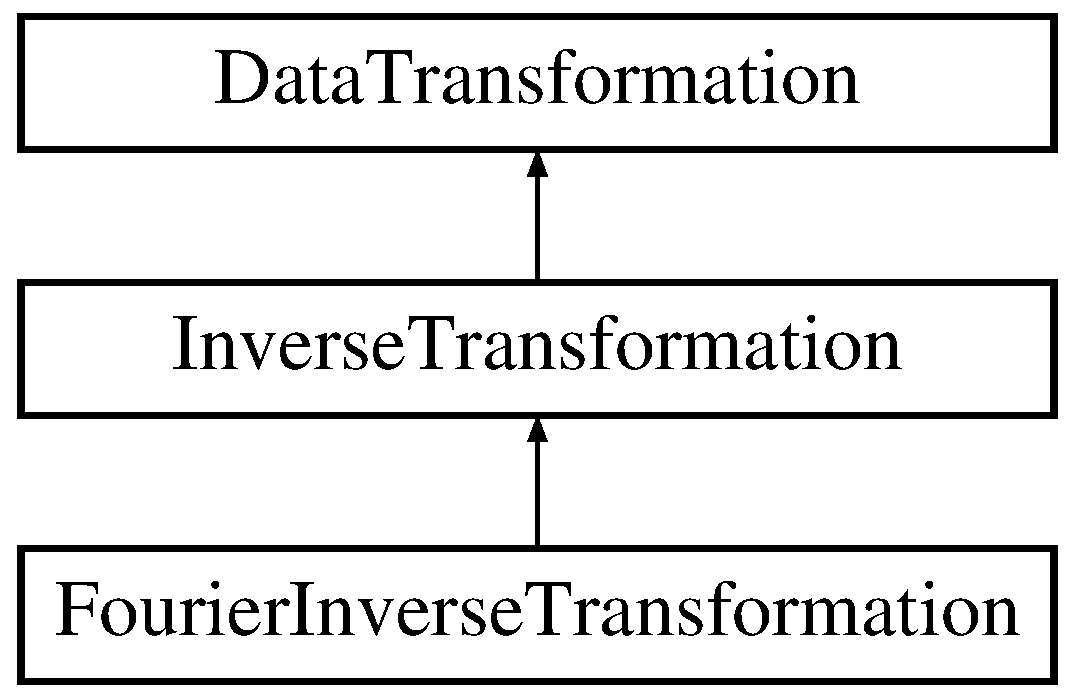
\includegraphics[height=3.000000cm]{classPecos_1_1FourierInverseTransformation}
\end{center}
\end{figure}
\subsection*{Public Member Functions}
\begin{DoxyCompactItemize}
\item 
\hyperlink{classPecos_1_1FourierInverseTransformation_afde642f63e26faafbe247b43d85c808a}{Fourier\+Inverse\+Transformation} (const String \&data\+\_\+trans\+\_\+type)\label{classPecos_1_1FourierInverseTransformation_afde642f63e26faafbe247b43d85c808a}

\begin{DoxyCompactList}\small\item\em constructor \end{DoxyCompactList}\item 
\hyperlink{classPecos_1_1FourierInverseTransformation_a92f432dd2b7c6c5d31b64ddaf0f20fc2}{$\sim$\+Fourier\+Inverse\+Transformation} ()\label{classPecos_1_1FourierInverseTransformation_a92f432dd2b7c6c5d31b64ddaf0f20fc2}

\begin{DoxyCompactList}\small\item\em destructor \end{DoxyCompactList}\end{DoxyCompactItemize}
\subsection*{Protected Member Functions}
\begin{DoxyCompactItemize}
\item 
void \hyperlink{classPecos_1_1FourierInverseTransformation_aff7310eaa8322a3eccf9815cc7da4a8e}{initialize} (const Real \&total\+\_\+t, const Real \&w\+\_\+bar, size\+\_\+t seed)\label{classPecos_1_1FourierInverseTransformation_aff7310eaa8322a3eccf9815cc7da4a8e}

\begin{DoxyCompactList}\small\item\em set scalar data \end{DoxyCompactList}\item 
void \hyperlink{classPecos_1_1FourierInverseTransformation_a2f54b6bae76157d4a964cd3ff73e4947}{power\+\_\+spectral\+\_\+density} (const String \&psd\+\_\+name, const Real \&param=0.)
\item 
const Real\+Vector \& \hyperlink{classPecos_1_1FourierInverseTransformation_a1e56233ae21533f04a96a94d7fa96786}{compute\+\_\+sample} ()\label{classPecos_1_1FourierInverseTransformation_a1e56233ae21533f04a96a94d7fa96786}

\begin{DoxyCompactList}\small\item\em compute and return \hyperlink{classPecos_1_1InverseTransformation_a17018c54acd67607b74c8783997d43a9}{Inverse\+Transformation\+::inverse\+Sample} \end{DoxyCompactList}\item 
const Real\+Matrix \& \hyperlink{classPecos_1_1FourierInverseTransformation_ac13e278177979d4ac4ae170a804e1ba7}{compute\+\_\+samples} (size\+\_\+t num\+\_\+ifft\+\_\+samples)\label{classPecos_1_1FourierInverseTransformation_ac13e278177979d4ac4ae170a804e1ba7}

\begin{DoxyCompactList}\small\item\em compute and return \hyperlink{classPecos_1_1InverseTransformation_ab9922b4f4d5024622225f70ea343f9ee}{Inverse\+Transformation\+::inverse\+Samples} \end{DoxyCompactList}\end{DoxyCompactItemize}
\subsection*{Private Member Functions}
\begin{DoxyCompactItemize}
\item 
void \hyperlink{classPecos_1_1FourierInverseTransformation_af228684696032356c68ba303e94ee62e}{compute\+\_\+sample\+\_\+shinozuka\+\_\+deodatis} ()\label{classPecos_1_1FourierInverseTransformation_af228684696032356c68ba303e94ee62e}

\begin{DoxyCompactList}\small\item\em perform i\+F\+FT using Shinozuka-\/\+Deodatis algorithm \end{DoxyCompactList}\item 
void \hyperlink{classPecos_1_1FourierInverseTransformation_a0f1ace07fbca48713f0a77b991d9f587}{compute\+\_\+sample\+\_\+grigoriu} ()\label{classPecos_1_1FourierInverseTransformation_a0f1ace07fbca48713f0a77b991d9f587}

\begin{DoxyCompactList}\small\item\em perform i\+F\+FT using Grigoriu algorithm \end{DoxyCompactList}\item 
void \hyperlink{classPecos_1_1FourierInverseTransformation_acf1c8578a2e83941e716ea08163ed0fc}{compute\+\_\+ifft\+\_\+sample\+\_\+set} (Complex\+Vector \&ifft\+\_\+vector)\label{classPecos_1_1FourierInverseTransformation_acf1c8578a2e83941e716ea08163ed0fc}

\begin{DoxyCompactList}\small\item\em use D\+F\+F\+T\+P\+A\+CK or F\+F\+TW to map B vector into the i-\/th inverse\+Samples vector \end{DoxyCompactList}\item 
void \hyperlink{classPecos_1_1FourierInverseTransformation_a32d626626eee0bc4ade146973f6abb1c}{finalize} ()\label{classPecos_1_1FourierInverseTransformation_a32d626626eee0bc4ade146973f6abb1c}

\begin{DoxyCompactList}\small\item\em deallocate data allocated in \hyperlink{classPecos_1_1FourierInverseTransformation_aff7310eaa8322a3eccf9815cc7da4a8e}{initialize()} \end{DoxyCompactList}\end{DoxyCompactItemize}
\subsection*{Private Attributes}
\begin{DoxyCompactItemize}
\item 
short \hyperlink{classPecos_1_1FourierInverseTransformation_a2bdf8e4836528f537931c346251891c0}{fourier\+Method}\label{classPecos_1_1FourierInverseTransformation_a2bdf8e4836528f537931c346251891c0}

\begin{DoxyCompactList}\small\item\em i\+F\+FT approach\+: I\+F\+F\+T\+\_\+\+SD (Shinozuka-\/\+Deodatis) or I\+F\+F\+T\+\_\+G (Grigoriu) \end{DoxyCompactList}\item 
size\+\_\+t \hyperlink{classPecos_1_1FourierInverseTransformation_a1b5d0d6b615c21f4d3accdc976c69290}{ifft\+Sample\+Cntr}\label{classPecos_1_1FourierInverseTransformation_a1b5d0d6b615c21f4d3accdc976c69290}

\begin{DoxyCompactList}\small\item\em counter for number of I\+F\+FT time domain realizations \end{DoxyCompactList}\item 
Real\+Vector \hyperlink{classPecos_1_1FourierInverseTransformation_a0a44b0cf49c6dbeb0ad7829dc7ae869e}{sigma\+Sequence}\label{classPecos_1_1FourierInverseTransformation_a0a44b0cf49c6dbeb0ad7829dc7ae869e}

\begin{DoxyCompactList}\small\item\em sequence of standard deviations computed from psd\+Sequence \end{DoxyCompactList}\item 
Complex\+Vector \hyperlink{classPecos_1_1FourierInverseTransformation_af39d7ad1911f4e0b35f223ea3891312f}{ifft\+Vector}\label{classPecos_1_1FourierInverseTransformation_af39d7ad1911f4e0b35f223ea3891312f}

\begin{DoxyCompactList}\small\item\em the complex vector passed through F\+F\+T\+W/\+D\+F\+F\+T\+P\+A\+CK for I\+F\+FT conversion from frequency domain to time domain \end{DoxyCompactList}\item 
Real\+Vector \hyperlink{classPecos_1_1FourierInverseTransformation_abf42c3f3fb4b853dccd6fc8702f1a45a}{lhs\+Param1}\label{classPecos_1_1FourierInverseTransformation_abf42c3f3fb4b853dccd6fc8702f1a45a}

\begin{DoxyCompactList}\small\item\em first L\+HS parameter vector (means for generate\+\_\+normal\+\_\+samples(), lower bounds for generate\+\_\+uniform\+\_\+samples()) \end{DoxyCompactList}\item 
Real\+Vector \hyperlink{classPecos_1_1FourierInverseTransformation_aeacf1f87e6b3e33d4fed439250089066}{lhs\+Param2}\label{classPecos_1_1FourierInverseTransformation_aeacf1f87e6b3e33d4fed439250089066}

\begin{DoxyCompactList}\small\item\em second L\+HS parameter vector (std devs for generate\+\_\+normal\+\_\+samples(), upper bounds for generate\+\_\+uniform\+\_\+samples()) \end{DoxyCompactList}\item 
Real\+Matrix \hyperlink{classPecos_1_1FourierInverseTransformation_a0ac2dc1881421113c2a365a6e306f1f9}{lhs\+Samples}\label{classPecos_1_1FourierInverseTransformation_a0ac2dc1881421113c2a365a6e306f1f9}

\begin{DoxyCompactList}\small\item\em random variable samples used in Grigoriu (num\+\_\+terms x 2 variables) and Shinozuka-\/\+Deodatis (num\+\_\+terms x 1 variable) algorithms \end{DoxyCompactList}\item 
fftw\+\_\+plan \hyperlink{classPecos_1_1FourierInverseTransformation_adc90e5fb3b914b14dc74e15e68d545dc}{fftw\+Plan}\label{classPecos_1_1FourierInverseTransformation_adc90e5fb3b914b14dc74e15e68d545dc}

\begin{DoxyCompactList}\small\item\em Plan cache for F\+F\+TW. \end{DoxyCompactList}\end{DoxyCompactItemize}
\subsection*{Additional Inherited Members}


\subsection{Detailed Description}
Class for i\+F\+FT data transformation. 

The \hyperlink{classPecos_1_1FourierInverseTransformation}{Fourier\+Inverse\+Transformation} employs an inverse fast Fourier transform (i\+F\+FT) to map from the frequency domain to the time domain. 

\subsection{Member Function Documentation}
\index{Pecos\+::\+Fourier\+Inverse\+Transformation@{Pecos\+::\+Fourier\+Inverse\+Transformation}!power\+\_\+spectral\+\_\+density@{power\+\_\+spectral\+\_\+density}}
\index{power\+\_\+spectral\+\_\+density@{power\+\_\+spectral\+\_\+density}!Pecos\+::\+Fourier\+Inverse\+Transformation@{Pecos\+::\+Fourier\+Inverse\+Transformation}}
\subsubsection[{\texorpdfstring{power\+\_\+spectral\+\_\+density(const String \&psd\+\_\+name, const Real \&param=0.)}{power_spectral_density(const String &psd_name, const Real &param=0.)}}]{\setlength{\rightskip}{0pt plus 5cm}void power\+\_\+spectral\+\_\+density (
\begin{DoxyParamCaption}
\item[{const String \&}]{psd\+\_\+name, }
\item[{const Real \&}]{param = {\ttfamily 0.}}
\end{DoxyParamCaption}
)\hspace{0.3cm}{\ttfamily [protected]}, {\ttfamily [virtual]}}\label{classPecos_1_1FourierInverseTransformation_a2f54b6bae76157d4a964cd3ff73e4947}
Augments \hyperlink{classPecos_1_1InverseTransformation_a2f54b6bae76157d4a964cd3ff73e4947}{Inverse\+Transformation\+::power\+\_\+spectral\+\_\+density()} definition to include local data initialization (sigma\+Sequence). 

Reimplemented from \hyperlink{classPecos_1_1DataTransformation_a2f54b6bae76157d4a964cd3ff73e4947}{Data\+Transformation}.



References Inverse\+Transformation\+::delta\+Omega, Inverse\+Transformation\+::power\+\_\+spectral\+\_\+density(), Inverse\+Transformation\+::psd\+Sequence, and Fourier\+Inverse\+Transformation\+::sigma\+Sequence.



Referenced by Fourier\+Inverse\+Transformation\+::finalize().



The documentation for this class was generated from the following files\+:\begin{DoxyCompactItemize}
\item 
Fourier\+Inverse\+Transformation.\+hpp\item 
Fourier\+Inverse\+Transformation.\+cpp\end{DoxyCompactItemize}

\section{Frechet\+Random\+Variable Class Reference}
\label{classPecos_1_1FrechetRandomVariable}\index{Frechet\+Random\+Variable@{Frechet\+Random\+Variable}}


Derived random variable class for frechet random variables.  


Inheritance diagram for Frechet\+Random\+Variable\+:\begin{figure}[H]
\begin{center}
\leavevmode
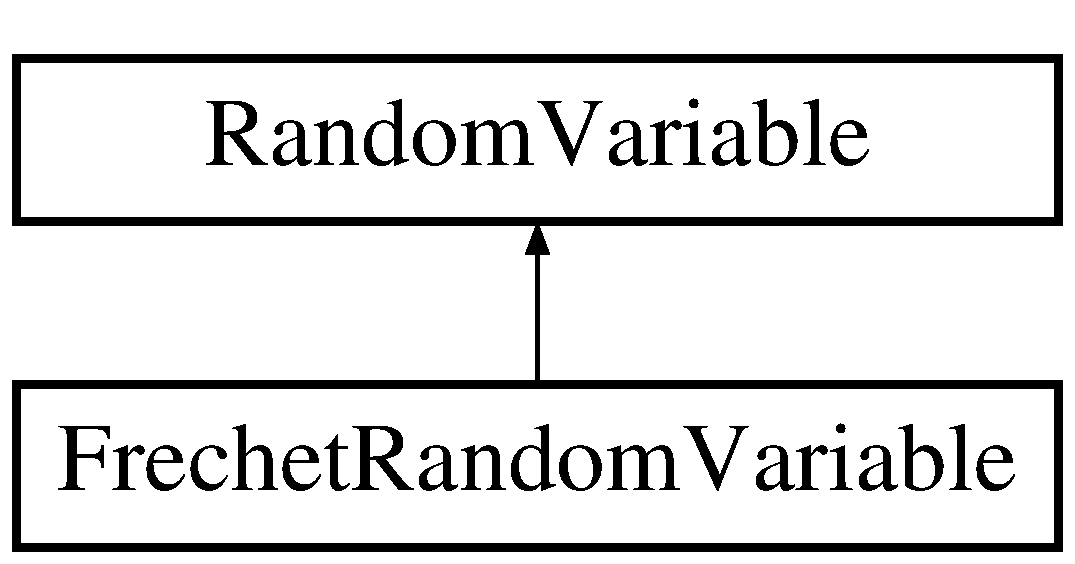
\includegraphics[height=2.000000cm]{classPecos_1_1FrechetRandomVariable}
\end{center}
\end{figure}
\subsection*{Public Member Functions}
\begin{DoxyCompactItemize}
\item 
\hyperlink{classPecos_1_1FrechetRandomVariable_ae4779be11834d22e5aabb3d4c8a4f9ca}{Frechet\+Random\+Variable} ()\label{classPecos_1_1FrechetRandomVariable_ae4779be11834d22e5aabb3d4c8a4f9ca}

\begin{DoxyCompactList}\small\item\em default constructor \end{DoxyCompactList}\item 
\hyperlink{classPecos_1_1FrechetRandomVariable_a80a163a727244db9fd1a5eae1bc2137d}{Frechet\+Random\+Variable} (Real alpha, Real beta)\label{classPecos_1_1FrechetRandomVariable_a80a163a727244db9fd1a5eae1bc2137d}

\begin{DoxyCompactList}\small\item\em alternate constructor \end{DoxyCompactList}\item 
\hyperlink{classPecos_1_1FrechetRandomVariable_a06711dd01877399b0637eb2fde1a13f2}{$\sim$\+Frechet\+Random\+Variable} ()\label{classPecos_1_1FrechetRandomVariable_a06711dd01877399b0637eb2fde1a13f2}

\begin{DoxyCompactList}\small\item\em destructor \end{DoxyCompactList}\item 
Real \hyperlink{classPecos_1_1FrechetRandomVariable_addd564e7f4f314e12d38df74d845f0d8}{cdf} (Real x) const \label{classPecos_1_1FrechetRandomVariable_addd564e7f4f314e12d38df74d845f0d8}

\begin{DoxyCompactList}\small\item\em return the cumulative distribution function value of the random variable at x \end{DoxyCompactList}\item 
Real \hyperlink{classPecos_1_1FrechetRandomVariable_a23c3b599e7e4788a9a5e9e93c3dbaf4d}{ccdf} (Real x) const \label{classPecos_1_1FrechetRandomVariable_a23c3b599e7e4788a9a5e9e93c3dbaf4d}

\begin{DoxyCompactList}\small\item\em return the complementary cumulative distribution function value of the random variable at x \end{DoxyCompactList}\item 
Real \hyperlink{classPecos_1_1FrechetRandomVariable_a918a1aac05ca349ea5313eebcba46c3e}{inverse\+\_\+cdf} (Real p\+\_\+cdf) const \label{classPecos_1_1FrechetRandomVariable_a918a1aac05ca349ea5313eebcba46c3e}

\begin{DoxyCompactList}\small\item\em return the x value corresponding to a cumulative probability \end{DoxyCompactList}\item 
Real \hyperlink{classPecos_1_1FrechetRandomVariable_afda003a1f59ff6930902cd5c8601f49b}{inverse\+\_\+ccdf} (Real p\+\_\+ccdf) const \label{classPecos_1_1FrechetRandomVariable_afda003a1f59ff6930902cd5c8601f49b}

\begin{DoxyCompactList}\small\item\em return the x value corresponding to a complementary cumulative probability \end{DoxyCompactList}\item 
Real \hyperlink{classPecos_1_1FrechetRandomVariable_a8ec69265f428e17c1707133cb137a819}{pdf} (Real x) const \label{classPecos_1_1FrechetRandomVariable_a8ec69265f428e17c1707133cb137a819}

\begin{DoxyCompactList}\small\item\em return the value of the random variable\textquotesingle{}s probability density function at x \end{DoxyCompactList}\item 
Real \hyperlink{classPecos_1_1FrechetRandomVariable_aaa7ca3718abc034be7629af5594efca0}{pdf\+\_\+gradient} (Real x) const \label{classPecos_1_1FrechetRandomVariable_aaa7ca3718abc034be7629af5594efca0}

\begin{DoxyCompactList}\small\item\em return the gradient of the random variable\textquotesingle{}s probability density function at x \end{DoxyCompactList}\item 
Real \hyperlink{classPecos_1_1FrechetRandomVariable_a6e2b6b6f13eedb2eb1ef3bc455a06392}{log\+\_\+pdf} (Real x) const \label{classPecos_1_1FrechetRandomVariable_a6e2b6b6f13eedb2eb1ef3bc455a06392}

\begin{DoxyCompactList}\small\item\em return the value of the natural log of the random variable\textquotesingle{}s probability density function at x (useful for calculations of log density in Bayesian methods) \end{DoxyCompactList}\item 
Real \hyperlink{classPecos_1_1FrechetRandomVariable_aa891dab1ae9a225f493e3a0e5032b778}{parameter} (short dist\+\_\+param) const \label{classPecos_1_1FrechetRandomVariable_aa891dab1ae9a225f493e3a0e5032b778}

\begin{DoxyCompactList}\small\item\em return the value of the named distribution parameter \end{DoxyCompactList}\item 
void \hyperlink{classPecos_1_1FrechetRandomVariable_ae8e123224f588aee676d5d56d5ca900d}{parameter} (short dist\+\_\+param, Real val)\label{classPecos_1_1FrechetRandomVariable_ae8e123224f588aee676d5d56d5ca900d}

\begin{DoxyCompactList}\small\item\em update the value of the named distribution parameter \end{DoxyCompactList}\item 
Real \hyperlink{classPecos_1_1FrechetRandomVariable_a962ffe5a3593be370d5c883365c060f4}{mean} () const \label{classPecos_1_1FrechetRandomVariable_a962ffe5a3593be370d5c883365c060f4}

\begin{DoxyCompactList}\small\item\em return the distribution mean \end{DoxyCompactList}\item 
Real \hyperlink{classPecos_1_1FrechetRandomVariable_ae1fff19ce29a79d657043a598523635d}{median} () const \label{classPecos_1_1FrechetRandomVariable_ae1fff19ce29a79d657043a598523635d}

\begin{DoxyCompactList}\small\item\em return the distribution mode \end{DoxyCompactList}\item 
Real \hyperlink{classPecos_1_1FrechetRandomVariable_a72d3d6926edd929cb3f8e12baa655f70}{mode} () const \label{classPecos_1_1FrechetRandomVariable_a72d3d6926edd929cb3f8e12baa655f70}

\begin{DoxyCompactList}\small\item\em return the distribution mode \end{DoxyCompactList}\item 
Real \hyperlink{classPecos_1_1FrechetRandomVariable_a6a4ed9624d511f8a4e4f509c82cb0706}{standard\+\_\+deviation} () const \label{classPecos_1_1FrechetRandomVariable_a6a4ed9624d511f8a4e4f509c82cb0706}

\begin{DoxyCompactList}\small\item\em return the distribution variance \end{DoxyCompactList}\item 
Real \hyperlink{classPecos_1_1FrechetRandomVariable_a4b8b05b2a9af92dad9cc304c2925a4eb}{variance} () const \label{classPecos_1_1FrechetRandomVariable_a4b8b05b2a9af92dad9cc304c2925a4eb}

\begin{DoxyCompactList}\small\item\em return the distribution variance \end{DoxyCompactList}\item 
Real\+Real\+Pair \hyperlink{classPecos_1_1FrechetRandomVariable_a4bdb95a8fa5fffaa0de5102f56963cf2}{bounds} () const \label{classPecos_1_1FrechetRandomVariable_a4bdb95a8fa5fffaa0de5102f56963cf2}

\begin{DoxyCompactList}\small\item\em return the distribution lower and upper bounds as a pair \end{DoxyCompactList}\item 
Real \hyperlink{classPecos_1_1FrechetRandomVariable_a9ee48b3ca93459136b2e73f77873c4aa}{correlation\+\_\+warping\+\_\+factor} (const \hyperlink{classPecos_1_1RandomVariable}{Random\+Variable} \&rv, Real corr) const \label{classPecos_1_1FrechetRandomVariable_a9ee48b3ca93459136b2e73f77873c4aa}

\begin{DoxyCompactList}\small\item\em compute the warping factor for correlation between the current variable and the one passed in (used in \hyperlink{classPecos_1_1NatafTransformation}{Nataf\+Transformation}) \end{DoxyCompactList}\item 
Real \hyperlink{classPecos_1_1FrechetRandomVariable_af889af8adfb262c9b74f573b2a9ffc99}{dx\+\_\+ds} (short dist\+\_\+param, short u\+\_\+type, Real x, Real z) const 
\item 
Real \hyperlink{classPecos_1_1FrechetRandomVariable_af6b5fc528523180bed5fc3008dcea205}{dz\+\_\+ds\+\_\+factor} (short u\+\_\+type, Real x, Real z) const 
\item 
void {\bfseries update} (Real alpha, Real beta)\label{classPecos_1_1FrechetRandomVariable_aaa82eccfdca4d440a4e2d4a890b0d9ed}

\item 
Real \hyperlink{classPecos_1_1FrechetRandomVariable_a065b031fb613138ede20895562efc61f}{inverse\+\_\+log\+\_\+cdf} (Real log\+\_\+p) const \label{classPecos_1_1FrechetRandomVariable_a065b031fb613138ede20895562efc61f}

\begin{DoxyCompactList}\small\item\em inactive Z\+\_\+to\+\_\+X mapping option in \hyperlink{classPecos_1_1NatafTransformation}{Nataf\+Transformation} \end{DoxyCompactList}\end{DoxyCompactItemize}
\subsection*{Static Public Member Functions}
\begin{DoxyCompactItemize}
\item 
static Real {\bfseries pdf} (Real x, Real alpha, Real beta)\label{classPecos_1_1FrechetRandomVariable_a739d94cef9ee188f00056e229ca3fd95}

\item 
static Real {\bfseries cdf} (Real x, Real alpha, Real beta)\label{classPecos_1_1FrechetRandomVariable_a6ccc276bca2bfdfd6f320c65a6c8aaf7}

\item 
static void {\bfseries moments\+\_\+from\+\_\+params} (Real alpha, Real beta, Real \&\hyperlink{classPecos_1_1FrechetRandomVariable_a962ffe5a3593be370d5c883365c060f4}{mean}, Real \&std\+\_\+dev)\label{classPecos_1_1FrechetRandomVariable_af6459b831a8e62a41f7eab34d06edad8}

\end{DoxyCompactItemize}
\subsection*{Protected Attributes}
\begin{DoxyCompactItemize}
\item 
Real \hyperlink{classPecos_1_1FrechetRandomVariable_aa48da95b9214d9cf933e1d4625e32e84}{alpha\+Stat}\label{classPecos_1_1FrechetRandomVariable_aa48da95b9214d9cf933e1d4625e32e84}

\begin{DoxyCompactList}\small\item\em alpha parameter of frechet random variable (shape) \end{DoxyCompactList}\item 
Real \hyperlink{classPecos_1_1FrechetRandomVariable_a838d220373c3360feec45e853b0daaac}{beta\+Stat}\label{classPecos_1_1FrechetRandomVariable_a838d220373c3360feec45e853b0daaac}

\begin{DoxyCompactList}\small\item\em beta parameter of frechet random variable (scale) \end{DoxyCompactList}\end{DoxyCompactItemize}
\subsection*{Additional Inherited Members}


\subsection{Detailed Description}
Derived random variable class for frechet random variables. 

Manages alpha and beta parameters. 

\subsection{Member Function Documentation}
\index{Pecos\+::\+Frechet\+Random\+Variable@{Pecos\+::\+Frechet\+Random\+Variable}!dx\+\_\+ds@{dx\+\_\+ds}}
\index{dx\+\_\+ds@{dx\+\_\+ds}!Pecos\+::\+Frechet\+Random\+Variable@{Pecos\+::\+Frechet\+Random\+Variable}}
\subsubsection[{\texorpdfstring{dx\+\_\+ds(short dist\+\_\+param, short u\+\_\+type, Real x, Real z) const }{dx_ds(short dist_param, short u_type, Real x, Real z) const }}]{\setlength{\rightskip}{0pt plus 5cm}Real dx\+\_\+ds (
\begin{DoxyParamCaption}
\item[{short}]{dist\+\_\+param, }
\item[{short}]{u\+\_\+type, }
\item[{Real}]{x, }
\item[{Real}]{z}
\end{DoxyParamCaption}
) const\hspace{0.3cm}{\ttfamily [inline]}, {\ttfamily [virtual]}}\label{classPecos_1_1FrechetRandomVariable_af889af8adfb262c9b74f573b2a9ffc99}
dx/ds is derived by differentiating \hyperlink{classPecos_1_1NatafTransformation_a5feeecf846fc017c5a28eccb4e955dc1}{Nataf\+Transformation\+::trans\+\_\+\+Z\+\_\+to\+\_\+\+X()} with respect to distribution parameter s. dz/ds is zero if uncorrelated, while \hyperlink{classPecos_1_1FrechetRandomVariable_af6b5fc528523180bed5fc3008dcea205}{dz\+\_\+ds\+\_\+factor()} manages contributions in the correlated case. 

Reimplemented from \hyperlink{classPecos_1_1RandomVariable_af889af8adfb262c9b74f573b2a9ffc99}{Random\+Variable}.



References Frechet\+Random\+Variable\+::alpha\+Stat, Frechet\+Random\+Variable\+::beta\+Stat, and Frechet\+Random\+Variable\+::dz\+\_\+ds\+\_\+factor().



Referenced by Frechet\+Random\+Variable\+::correlation\+\_\+warping\+\_\+factor().

\index{Pecos\+::\+Frechet\+Random\+Variable@{Pecos\+::\+Frechet\+Random\+Variable}!dz\+\_\+ds\+\_\+factor@{dz\+\_\+ds\+\_\+factor}}
\index{dz\+\_\+ds\+\_\+factor@{dz\+\_\+ds\+\_\+factor}!Pecos\+::\+Frechet\+Random\+Variable@{Pecos\+::\+Frechet\+Random\+Variable}}
\subsubsection[{\texorpdfstring{dz\+\_\+ds\+\_\+factor(short u\+\_\+type, Real x, Real z) const }{dz_ds_factor(short u_type, Real x, Real z) const }}]{\setlength{\rightskip}{0pt plus 5cm}Real dz\+\_\+ds\+\_\+factor (
\begin{DoxyParamCaption}
\item[{short}]{u\+\_\+type, }
\item[{Real}]{x, }
\item[{Real}]{z}
\end{DoxyParamCaption}
) const\hspace{0.3cm}{\ttfamily [inline]}, {\ttfamily [virtual]}}\label{classPecos_1_1FrechetRandomVariable_af6b5fc528523180bed5fc3008dcea205}
dx/ds is derived by differentiating \hyperlink{classPecos_1_1NatafTransformation_a5feeecf846fc017c5a28eccb4e955dc1}{Nataf\+Transformation\+::trans\+\_\+\+Z\+\_\+to\+\_\+\+X()} with respect to distribution parameter s. For the uncorrelated case, u and z are constants. For the correlated case, u is a constant, but z(s) = L(s) u due to Nataf dependence on s and dz/ds = d\+L/ds u. 

Reimplemented from \hyperlink{classPecos_1_1RandomVariable_af6b5fc528523180bed5fc3008dcea205}{Random\+Variable}.



References Frechet\+Random\+Variable\+::alpha\+Stat, Frechet\+Random\+Variable\+::beta\+Stat, Frechet\+Random\+Variable\+::cdf(), Frechet\+Random\+Variable\+::mean(), Frechet\+Random\+Variable\+::pdf(), Normal\+Random\+Variable\+::std\+\_\+cdf(), and Normal\+Random\+Variable\+::std\+\_\+pdf().



Referenced by Frechet\+Random\+Variable\+::dx\+\_\+ds().



The documentation for this class was generated from the following file\+:\begin{DoxyCompactItemize}
\item 
Frechet\+Random\+Variable.\+hpp\end{DoxyCompactItemize}

\section{Gamma\+Random\+Variable Class Reference}
\label{classPecos_1_1GammaRandomVariable}\index{Gamma\+Random\+Variable@{Gamma\+Random\+Variable}}


Derived random variable class for gamma random variables.  


Inheritance diagram for Gamma\+Random\+Variable\+:\begin{figure}[H]
\begin{center}
\leavevmode
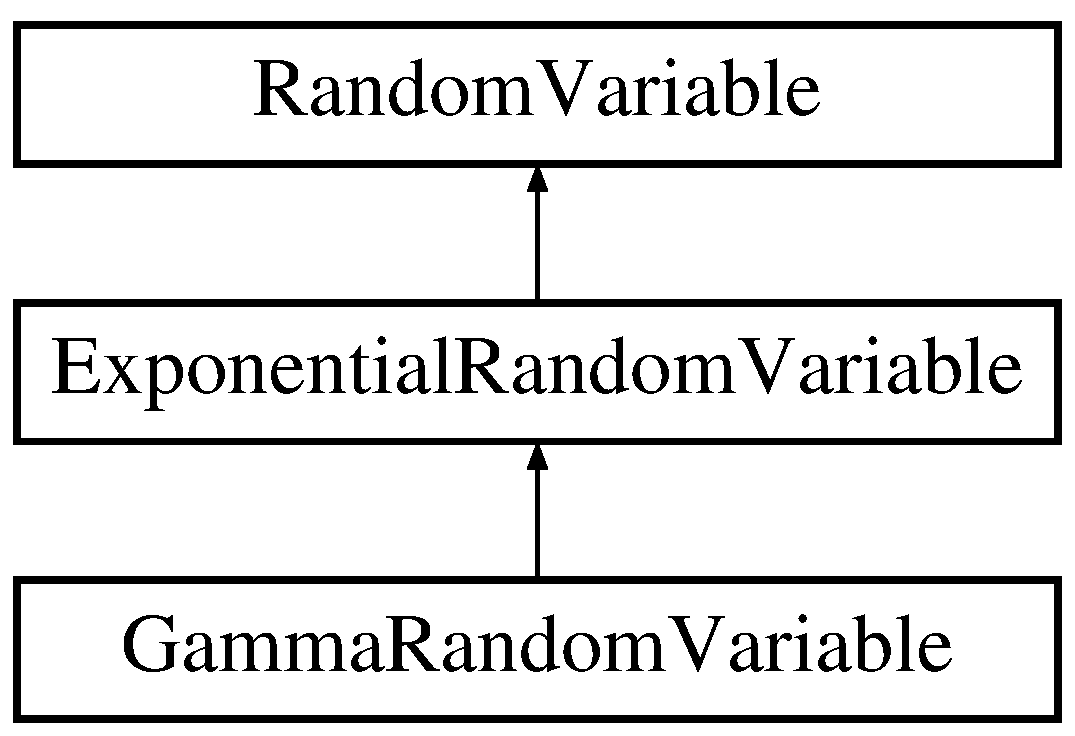
\includegraphics[height=3.000000cm]{classPecos_1_1GammaRandomVariable}
\end{center}
\end{figure}
\subsection*{Public Member Functions}
\begin{DoxyCompactItemize}
\item 
\hyperlink{classPecos_1_1GammaRandomVariable_ab20e31c6e009624c92e3e6dbc02101a9}{Gamma\+Random\+Variable} ()\label{classPecos_1_1GammaRandomVariable_ab20e31c6e009624c92e3e6dbc02101a9}

\begin{DoxyCompactList}\small\item\em default constructor \end{DoxyCompactList}\item 
\hyperlink{classPecos_1_1GammaRandomVariable_abfcee58f29493ea95cfface6997b8357}{Gamma\+Random\+Variable} (Real alpha, Real beta)\label{classPecos_1_1GammaRandomVariable_abfcee58f29493ea95cfface6997b8357}

\begin{DoxyCompactList}\small\item\em alternate constructor \end{DoxyCompactList}\item 
\hyperlink{classPecos_1_1GammaRandomVariable_a4b7e62bafb8df63c54960df9337933e7}{$\sim$\+Gamma\+Random\+Variable} ()\label{classPecos_1_1GammaRandomVariable_a4b7e62bafb8df63c54960df9337933e7}

\begin{DoxyCompactList}\small\item\em destructor \end{DoxyCompactList}\item 
Real \hyperlink{classPecos_1_1GammaRandomVariable_addd564e7f4f314e12d38df74d845f0d8}{cdf} (Real x) const \label{classPecos_1_1GammaRandomVariable_addd564e7f4f314e12d38df74d845f0d8}

\begin{DoxyCompactList}\small\item\em return the cumulative distribution function value of the random variable at x \end{DoxyCompactList}\item 
Real \hyperlink{classPecos_1_1GammaRandomVariable_a23c3b599e7e4788a9a5e9e93c3dbaf4d}{ccdf} (Real x) const \label{classPecos_1_1GammaRandomVariable_a23c3b599e7e4788a9a5e9e93c3dbaf4d}

\begin{DoxyCompactList}\small\item\em return the complementary cumulative distribution function value of the random variable at x \end{DoxyCompactList}\item 
Real \hyperlink{classPecos_1_1GammaRandomVariable_a918a1aac05ca349ea5313eebcba46c3e}{inverse\+\_\+cdf} (Real p\+\_\+cdf) const \label{classPecos_1_1GammaRandomVariable_a918a1aac05ca349ea5313eebcba46c3e}

\begin{DoxyCompactList}\small\item\em return the x value corresponding to a cumulative probability \end{DoxyCompactList}\item 
Real \hyperlink{classPecos_1_1GammaRandomVariable_afda003a1f59ff6930902cd5c8601f49b}{inverse\+\_\+ccdf} (Real p\+\_\+ccdf) const \label{classPecos_1_1GammaRandomVariable_afda003a1f59ff6930902cd5c8601f49b}

\begin{DoxyCompactList}\small\item\em return the x value corresponding to a complementary cumulative probability \end{DoxyCompactList}\item 
Real \hyperlink{classPecos_1_1GammaRandomVariable_a8ec69265f428e17c1707133cb137a819}{pdf} (Real x) const \label{classPecos_1_1GammaRandomVariable_a8ec69265f428e17c1707133cb137a819}

\begin{DoxyCompactList}\small\item\em return the value of the random variable\textquotesingle{}s probability density function at x \end{DoxyCompactList}\item 
Real \hyperlink{classPecos_1_1GammaRandomVariable_aaa7ca3718abc034be7629af5594efca0}{pdf\+\_\+gradient} (Real x) const \label{classPecos_1_1GammaRandomVariable_aaa7ca3718abc034be7629af5594efca0}

\begin{DoxyCompactList}\small\item\em return the gradient of the random variable\textquotesingle{}s probability density function at x \end{DoxyCompactList}\item 
Real \hyperlink{classPecos_1_1GammaRandomVariable_a514a0abe97269ac6e003f43683d9137e}{pdf\+\_\+hessian} (Real x) const \label{classPecos_1_1GammaRandomVariable_a514a0abe97269ac6e003f43683d9137e}

\begin{DoxyCompactList}\small\item\em return the hessian of the random variable\textquotesingle{}s probability density function at x \end{DoxyCompactList}\item 
Real \hyperlink{classPecos_1_1GammaRandomVariable_a6e2b6b6f13eedb2eb1ef3bc455a06392}{log\+\_\+pdf} (Real x) const \label{classPecos_1_1GammaRandomVariable_a6e2b6b6f13eedb2eb1ef3bc455a06392}

\begin{DoxyCompactList}\small\item\em return the value of the natural log of the random variable\textquotesingle{}s probability density function at x (useful for calculations of log density in Bayesian methods) \end{DoxyCompactList}\item 
Real \hyperlink{classPecos_1_1GammaRandomVariable_a5ccc16c04690f0c501f44c1ffae2bbd1}{log\+\_\+pdf\+\_\+gradient} (Real x) const \label{classPecos_1_1GammaRandomVariable_a5ccc16c04690f0c501f44c1ffae2bbd1}

\begin{DoxyCompactList}\small\item\em return the gradient of the natural log of the random variable\textquotesingle{}s probability density function at x (useful for defining M\+C\+MC proposal distributions in Bayesian methods) \end{DoxyCompactList}\item 
Real \hyperlink{classPecos_1_1GammaRandomVariable_a7b43f26f0f2bcdfef15d87e1f9399b33}{log\+\_\+pdf\+\_\+hessian} (Real x) const \label{classPecos_1_1GammaRandomVariable_a7b43f26f0f2bcdfef15d87e1f9399b33}

\begin{DoxyCompactList}\small\item\em return the Hessian of the natural log of the random variable\textquotesingle{}s probability density function at x (useful for defining M\+C\+MC proposal distributions in Bayesian methods) \end{DoxyCompactList}\item 
Real \hyperlink{classPecos_1_1GammaRandomVariable_acffcd338a207168a147fffe0778ccf3c}{inverse\+\_\+standard\+\_\+cdf} (Real p\+\_\+cdf) const \label{classPecos_1_1GammaRandomVariable_acffcd338a207168a147fffe0778ccf3c}

\begin{DoxyCompactList}\small\item\em return the x value for a standardized probability distribution corresponding to a cumulative probability \end{DoxyCompactList}\item 
Real \hyperlink{classPecos_1_1GammaRandomVariable_a206a02581b82f44be4a5321488a12daa}{standard\+\_\+pdf} (Real z) const \label{classPecos_1_1GammaRandomVariable_a206a02581b82f44be4a5321488a12daa}

\begin{DoxyCompactList}\small\item\em return the value of a standardized random variable\textquotesingle{}s probability density function at x \end{DoxyCompactList}\item 
Real \hyperlink{classPecos_1_1GammaRandomVariable_a1eb7deb350fc38d35e32ba7d0b96c464}{log\+\_\+standard\+\_\+pdf} (Real z) const \label{classPecos_1_1GammaRandomVariable_a1eb7deb350fc38d35e32ba7d0b96c464}

\begin{DoxyCompactList}\small\item\em return the natural log of a standardized random variable\textquotesingle{}s probability density function at x (useful for calculations of log density in Bayesian methods) \end{DoxyCompactList}\item 
Real \hyperlink{classPecos_1_1GammaRandomVariable_a73ea75d51f5415f600bebbca4a9628b7}{log\+\_\+standard\+\_\+pdf\+\_\+gradient} (Real z) const \label{classPecos_1_1GammaRandomVariable_a73ea75d51f5415f600bebbca4a9628b7}

\begin{DoxyCompactList}\small\item\em return the gradient of the natural log of a standardized random variable\textquotesingle{}s probability density function at x (useful for calculations of log density in Bayesian methods) \end{DoxyCompactList}\item 
Real \hyperlink{classPecos_1_1GammaRandomVariable_acf89562740c674e54901e97817f56b69}{log\+\_\+standard\+\_\+pdf\+\_\+hessian} (Real z) const \label{classPecos_1_1GammaRandomVariable_acf89562740c674e54901e97817f56b69}

\begin{DoxyCompactList}\small\item\em return the Hessian of the natural log of a standardized random variable\textquotesingle{}s probability density function at x (useful for calculations of log density in Bayesian methods) \end{DoxyCompactList}\item 
Real \hyperlink{classPecos_1_1GammaRandomVariable_aa891dab1ae9a225f493e3a0e5032b778}{parameter} (short dist\+\_\+param) const \label{classPecos_1_1GammaRandomVariable_aa891dab1ae9a225f493e3a0e5032b778}

\begin{DoxyCompactList}\small\item\em return the value of the named distribution parameter \end{DoxyCompactList}\item 
void \hyperlink{classPecos_1_1GammaRandomVariable_ae8e123224f588aee676d5d56d5ca900d}{parameter} (short dist\+\_\+param, Real val)\label{classPecos_1_1GammaRandomVariable_ae8e123224f588aee676d5d56d5ca900d}

\begin{DoxyCompactList}\small\item\em update the value of the named distribution parameter \end{DoxyCompactList}\item 
Real \hyperlink{classPecos_1_1GammaRandomVariable_a962ffe5a3593be370d5c883365c060f4}{mean} () const \label{classPecos_1_1GammaRandomVariable_a962ffe5a3593be370d5c883365c060f4}

\begin{DoxyCompactList}\small\item\em return the distribution mean \end{DoxyCompactList}\item 
Real \hyperlink{classPecos_1_1GammaRandomVariable_ae1fff19ce29a79d657043a598523635d}{median} () const \label{classPecos_1_1GammaRandomVariable_ae1fff19ce29a79d657043a598523635d}

\begin{DoxyCompactList}\small\item\em return the distribution mode \end{DoxyCompactList}\item 
Real \hyperlink{classPecos_1_1GammaRandomVariable_a72d3d6926edd929cb3f8e12baa655f70}{mode} () const \label{classPecos_1_1GammaRandomVariable_a72d3d6926edd929cb3f8e12baa655f70}

\begin{DoxyCompactList}\small\item\em return the distribution mode \end{DoxyCompactList}\item 
Real \hyperlink{classPecos_1_1GammaRandomVariable_a6a4ed9624d511f8a4e4f509c82cb0706}{standard\+\_\+deviation} () const \label{classPecos_1_1GammaRandomVariable_a6a4ed9624d511f8a4e4f509c82cb0706}

\begin{DoxyCompactList}\small\item\em return the distribution variance \end{DoxyCompactList}\item 
Real \hyperlink{classPecos_1_1GammaRandomVariable_a4b8b05b2a9af92dad9cc304c2925a4eb}{variance} () const \label{classPecos_1_1GammaRandomVariable_a4b8b05b2a9af92dad9cc304c2925a4eb}

\begin{DoxyCompactList}\small\item\em return the distribution variance \end{DoxyCompactList}\item 
Real \hyperlink{classPecos_1_1GammaRandomVariable_a9ee48b3ca93459136b2e73f77873c4aa}{correlation\+\_\+warping\+\_\+factor} (const \hyperlink{classPecos_1_1RandomVariable}{Random\+Variable} \&rv, Real corr) const \label{classPecos_1_1GammaRandomVariable_a9ee48b3ca93459136b2e73f77873c4aa}

\begin{DoxyCompactList}\small\item\em compute the warping factor for correlation between the current variable and the one passed in (used in \hyperlink{classPecos_1_1NatafTransformation}{Nataf\+Transformation}) \end{DoxyCompactList}\item 
Real \hyperlink{classPecos_1_1GammaRandomVariable_af889af8adfb262c9b74f573b2a9ffc99}{dx\+\_\+ds} (short dist\+\_\+param, short u\+\_\+type, Real x, Real z) const 
\item 
Real \hyperlink{classPecos_1_1GammaRandomVariable_af6b5fc528523180bed5fc3008dcea205}{dz\+\_\+ds\+\_\+factor} (short u\+\_\+type, Real x, Real z) const 
\item 
void {\bfseries update} (Real alpha, Real beta)\label{classPecos_1_1GammaRandomVariable_aaa82eccfdca4d440a4e2d4a890b0d9ed}

\end{DoxyCompactItemize}
\subsection*{Static Public Member Functions}
\begin{DoxyCompactItemize}
\item 
static Real {\bfseries pdf} (Real x, Real alpha, Real beta)\label{classPecos_1_1GammaRandomVariable_a739d94cef9ee188f00056e229ca3fd95}

\item 
static Real {\bfseries cdf} (Real x, Real alpha, Real beta)\label{classPecos_1_1GammaRandomVariable_a6ccc276bca2bfdfd6f320c65a6c8aaf7}

\item 
static Real {\bfseries inverse\+\_\+cdf} (Real \hyperlink{classPecos_1_1GammaRandomVariable_addd564e7f4f314e12d38df74d845f0d8}{cdf}, Real alpha, Real beta)\label{classPecos_1_1GammaRandomVariable_a2e77b37ec653326d8c6189a646b8db7b}

\item 
static void {\bfseries moments\+\_\+from\+\_\+params} (Real alpha, Real beta, Real \&\hyperlink{classPecos_1_1GammaRandomVariable_a962ffe5a3593be370d5c883365c060f4}{mean}, Real \&std\+\_\+dev)\label{classPecos_1_1GammaRandomVariable_af6459b831a8e62a41f7eab34d06edad8}

\end{DoxyCompactItemize}
\subsection*{Protected Member Functions}
\begin{DoxyCompactItemize}
\item 
void \hyperlink{classPecos_1_1GammaRandomVariable_aaa6750cbee2245416a6eeeac58d4405a}{update\+\_\+boost} ()\label{classPecos_1_1GammaRandomVariable_aaa6750cbee2245416a6eeeac58d4405a}

\begin{DoxyCompactList}\small\item\em create a new gamma\+Dist instance \end{DoxyCompactList}\end{DoxyCompactItemize}
\subsection*{Protected Attributes}
\begin{DoxyCompactItemize}
\item 
Real \hyperlink{classPecos_1_1GammaRandomVariable_af2fa8d657b4ae8750d30b09f10760799}{alpha\+Shape}\label{classPecos_1_1GammaRandomVariable_af2fa8d657b4ae8750d30b09f10760799}

\begin{DoxyCompactList}\small\item\em alpha shape parameter of gamma random variable (statistical P\+DF convention; differs from Gen\+Laguerre polynomial convention) \end{DoxyCompactList}\item 
gamma\+\_\+dist $\ast$ \hyperlink{classPecos_1_1GammaRandomVariable_a284f48d0d01e3e0acf2cd606fab6f71d}{gamma\+Dist}\label{classPecos_1_1GammaRandomVariable_a284f48d0d01e3e0acf2cd606fab6f71d}

\begin{DoxyCompactList}\small\item\em pointer to the Boost gamma\+\_\+distribution instance \end{DoxyCompactList}\end{DoxyCompactItemize}


\subsection{Detailed Description}
Derived random variable class for gamma random variables. 

Manages alpha and inherits beta. This follows the Gamma(alpha,beta) definition in Law \& Kelton, which differs from the L\+HS definition (beta\+\_\+\+LK = 1/beta\+\_\+\+L\+HS). 

\subsection{Member Function Documentation}
\index{Pecos\+::\+Gamma\+Random\+Variable@{Pecos\+::\+Gamma\+Random\+Variable}!dx\+\_\+ds@{dx\+\_\+ds}}
\index{dx\+\_\+ds@{dx\+\_\+ds}!Pecos\+::\+Gamma\+Random\+Variable@{Pecos\+::\+Gamma\+Random\+Variable}}
\subsubsection[{\texorpdfstring{dx\+\_\+ds(short dist\+\_\+param, short u\+\_\+type, Real x, Real z) const }{dx_ds(short dist_param, short u_type, Real x, Real z) const }}]{\setlength{\rightskip}{0pt plus 5cm}Real dx\+\_\+ds (
\begin{DoxyParamCaption}
\item[{short}]{dist\+\_\+param, }
\item[{short}]{u\+\_\+type, }
\item[{Real}]{x, }
\item[{Real}]{z}
\end{DoxyParamCaption}
) const\hspace{0.3cm}{\ttfamily [inline]}, {\ttfamily [virtual]}}\label{classPecos_1_1GammaRandomVariable_af889af8adfb262c9b74f573b2a9ffc99}
dx/ds is derived by differentiating \hyperlink{classPecos_1_1NatafTransformation_a5feeecf846fc017c5a28eccb4e955dc1}{Nataf\+Transformation\+::trans\+\_\+\+Z\+\_\+to\+\_\+\+X()} with respect to distribution parameter s. dz/ds is zero if uncorrelated, while \hyperlink{classPecos_1_1GammaRandomVariable_af6b5fc528523180bed5fc3008dcea205}{dz\+\_\+ds\+\_\+factor()} manages contributions in the correlated case. 

Reimplemented from \hyperlink{classPecos_1_1ExponentialRandomVariable_af889af8adfb262c9b74f573b2a9ffc99}{Exponential\+Random\+Variable}.



References Gamma\+Random\+Variable\+::dz\+\_\+ds\+\_\+factor().



Referenced by Gamma\+Random\+Variable\+::correlation\+\_\+warping\+\_\+factor().

\index{Pecos\+::\+Gamma\+Random\+Variable@{Pecos\+::\+Gamma\+Random\+Variable}!dz\+\_\+ds\+\_\+factor@{dz\+\_\+ds\+\_\+factor}}
\index{dz\+\_\+ds\+\_\+factor@{dz\+\_\+ds\+\_\+factor}!Pecos\+::\+Gamma\+Random\+Variable@{Pecos\+::\+Gamma\+Random\+Variable}}
\subsubsection[{\texorpdfstring{dz\+\_\+ds\+\_\+factor(short u\+\_\+type, Real x, Real z) const }{dz_ds_factor(short u_type, Real x, Real z) const }}]{\setlength{\rightskip}{0pt plus 5cm}Real dz\+\_\+ds\+\_\+factor (
\begin{DoxyParamCaption}
\item[{short}]{u\+\_\+type, }
\item[{Real}]{x, }
\item[{Real}]{z}
\end{DoxyParamCaption}
) const\hspace{0.3cm}{\ttfamily [inline]}, {\ttfamily [virtual]}}\label{classPecos_1_1GammaRandomVariable_af6b5fc528523180bed5fc3008dcea205}
dx/ds is derived by differentiating \hyperlink{classPecos_1_1NatafTransformation_a5feeecf846fc017c5a28eccb4e955dc1}{Nataf\+Transformation\+::trans\+\_\+\+Z\+\_\+to\+\_\+\+X()} with respect to distribution parameter s. For the uncorrelated case, u and z are constants. For the correlated case, u is a constant, but z(s) = L(s) u due to Nataf dependence on s and dz/ds = d\+L/ds u. 

Reimplemented from \hyperlink{classPecos_1_1ExponentialRandomVariable_af6b5fc528523180bed5fc3008dcea205}{Exponential\+Random\+Variable}.



References Exponential\+Random\+Variable\+::beta\+Scale.



Referenced by Gamma\+Random\+Variable\+::dx\+\_\+ds().



The documentation for this class was generated from the following file\+:\begin{DoxyCompactItemize}
\item 
Gamma\+Random\+Variable.\+hpp\end{DoxyCompactItemize}

\section{Gaussian\+K\+DE Class Reference}
\label{classPecos_1_1GaussianKDE}\index{Gaussian\+K\+DE@{Gaussian\+K\+DE}}


Class for kernel density estimation with gaussian kernels.  


Inheritance diagram for Gaussian\+K\+DE\+:\begin{figure}[H]
\begin{center}
\leavevmode
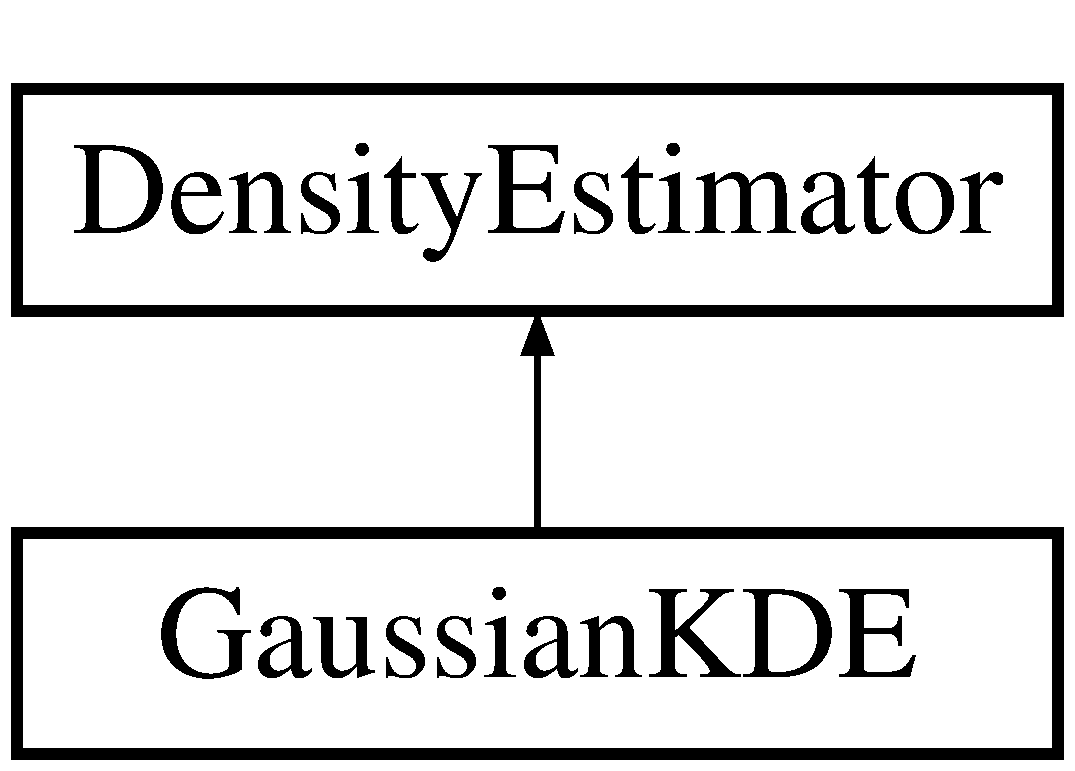
\includegraphics[height=2.000000cm]{classPecos_1_1GaussianKDE}
\end{center}
\end{figure}
\subsection*{Public Member Functions}
\begin{DoxyCompactItemize}
\item 
\hyperlink{classPecos_1_1GaussianKDE_a9c2a04bf8270c1ffa8dae1f04cc80b61}{Gaussian\+K\+DE} ()\label{classPecos_1_1GaussianKDE_a9c2a04bf8270c1ffa8dae1f04cc80b61}

\begin{DoxyCompactList}\small\item\em default constructor \end{DoxyCompactList}\item 
\hyperlink{classPecos_1_1GaussianKDE_a976d463a5f7d52ad04814a44228a0751}{$\sim$\+Gaussian\+K\+DE} ()\label{classPecos_1_1GaussianKDE_a976d463a5f7d52ad04814a44228a0751}

\begin{DoxyCompactList}\small\item\em destructor \end{DoxyCompactList}\item 
void \hyperlink{classPecos_1_1GaussianKDE_a6c7e188a789efc33dbeb356f6e200c33}{initialize} (Real\+Matrix \&samples, Teuchos\+::\+E\+Transp trans=Teuchos\+::\+N\+O\+\_\+\+T\+R\+A\+NS)\label{classPecos_1_1GaussianKDE_a6c7e188a789efc33dbeb356f6e200c33}

\begin{DoxyCompactList}\small\item\em initialize the density estimator \end{DoxyCompactList}\item 
void {\bfseries initialize} (Real\+Vector\+Array \&samples)\label{classPecos_1_1GaussianKDE_a50fd0e9c6addf748bf7ae040ec0d91f9}

\item 
size\+\_\+t \hyperlink{classPecos_1_1GaussianKDE_a890ccac161f0becd266252b4cd3b9584}{get\+Dim} ()\label{classPecos_1_1GaussianKDE_a890ccac161f0becd266252b4cd3b9584}

\begin{DoxyCompactList}\small\item\em get the dimensionality \end{DoxyCompactList}\item 
Real \hyperlink{classPecos_1_1GaussianKDE_adc6f262952d05a33ff68cae37929cbb2}{mean} ()\label{classPecos_1_1GaussianKDE_adc6f262952d05a33ff68cae37929cbb2}

\begin{DoxyCompactList}\small\item\em computes the sample mean \end{DoxyCompactList}\item 
Real \hyperlink{classPecos_1_1GaussianKDE_a38f6da77468be17e02ce38af2c0976c3}{variance} ()\label{classPecos_1_1GaussianKDE_a38f6da77468be17e02ce38af2c0976c3}

\begin{DoxyCompactList}\small\item\em computed according to \mbox{[}Goodman, 1962\mbox{]} \end{DoxyCompactList}\item 
Real \hyperlink{classPecos_1_1GaussianKDE_a3e3c923ec6be63011f72bb65b08789ed}{std\+\_\+deviation} ()\label{classPecos_1_1GaussianKDE_a3e3c923ec6be63011f72bb65b08789ed}

\begin{DoxyCompactList}\small\item\em computes the standard deviation \end{DoxyCompactList}\item 
void \hyperlink{classPecos_1_1GaussianKDE_a8cf84ab65e0bccb16f5cdbccc9790dc9}{cov} (Real\+Matrix \&cov)\label{classPecos_1_1GaussianKDE_a8cf84ab65e0bccb16f5cdbccc9790dc9}

\begin{DoxyCompactList}\small\item\em computes the covariance matrix \end{DoxyCompactList}\item 
Real \hyperlink{classPecos_1_1GaussianKDE_ae49fd0166d0cedd899f933e3e2b713aa}{pdf} (const Real\+Vector \&x) const \label{classPecos_1_1GaussianKDE_ae49fd0166d0cedd899f933e3e2b713aa}

\begin{DoxyCompactList}\small\item\em operations for single samples \end{DoxyCompactList}\item 
void \hyperlink{classPecos_1_1GaussianKDE_a83ef7a2b0cf786922fbdfb17d284d2e0}{pdf} (const Real\+Matrix \&data, Real\+Vector \&res, Teuchos\+::\+E\+Transp trans=Teuchos\+::\+N\+O\+\_\+\+T\+R\+A\+NS) const \label{classPecos_1_1GaussianKDE_a83ef7a2b0cf786922fbdfb17d284d2e0}

\begin{DoxyCompactList}\small\item\em operations for a set of samples \end{DoxyCompactList}\item 
virtual void \hyperlink{classPecos_1_1GaussianKDE_a5aa525959e7bee8034a26a77e00f12ef}{marginalize} (size\+\_\+t dim, \hyperlink{classPecos_1_1DensityEstimator}{Density\+Estimator} \&estimator)\label{classPecos_1_1GaussianKDE_a5aa525959e7bee8034a26a77e00f12ef}

\begin{DoxyCompactList}\small\item\em marginalization operations \end{DoxyCompactList}\item 
virtual void \hyperlink{classPecos_1_1GaussianKDE_a50f735eabae41f8948d792ac84749095}{marg\+To\+Dim\+Xs} (const Int\+Vector \&dims, \hyperlink{classPecos_1_1DensityEstimator}{Density\+Estimator} \&estimator)\label{classPecos_1_1GaussianKDE_a50f735eabae41f8948d792ac84749095}

\begin{DoxyCompactList}\small\item\em creates a maginalized density with remaining dims \end{DoxyCompactList}\item 
virtual void \hyperlink{classPecos_1_1GaussianKDE_ab1e735a6e2e62abfaa78e44d3a6bd9ec}{marg\+To\+DimX} (size\+\_\+t dim, \hyperlink{classPecos_1_1DensityEstimator}{Density\+Estimator} \&estimator)\label{classPecos_1_1GaussianKDE_ab1e735a6e2e62abfaa78e44d3a6bd9ec}

\begin{DoxyCompactList}\small\item\em creates a maginalized density with one remaining dimension \end{DoxyCompactList}\item 
virtual void \hyperlink{classPecos_1_1GaussianKDE_a48a43dfe8975d003c2c7cff695046414}{conditionalize} (const Real\+Vector \&x, const Int\+Vector \&dims, \hyperlink{classPecos_1_1DensityEstimator}{Density\+Estimator} \&estimator)\label{classPecos_1_1GaussianKDE_a48a43dfe8975d003c2c7cff695046414}

\begin{DoxyCompactList}\small\item\em conditionalization operations \end{DoxyCompactList}\item 
virtual void {\bfseries cond\+To\+DimX} (const Real\+Vector \&x, size\+\_\+t dim, \hyperlink{classPecos_1_1DensityEstimator}{Density\+Estimator} \&estimator)\label{classPecos_1_1GaussianKDE_aa4b4c620def1d4611d3e10dcd4b3a073}

\item 
void \hyperlink{classPecos_1_1GaussianKDE_a795359a100b6b2113637ae2d0c6cd148}{get\+Conditionalization\+Factor} (Real\+Vector \&pcond)\label{classPecos_1_1GaussianKDE_a795359a100b6b2113637ae2d0c6cd148}

\begin{DoxyCompactList}\small\item\em getter and setter functions \end{DoxyCompactList}\item 
void {\bfseries set\+Conditionalization\+Factor} (const Real\+Vector \&pcond)\label{classPecos_1_1GaussianKDE_a680bc5e5333d94f3c342d99c501a43eb}

\item 
void {\bfseries get\+Bandwidths} (Real\+Vector \&\hyperlink{classPecos_1_1GaussianKDE_ae303fb49034fb553ad86c64be017915f}{bandwidths})\label{classPecos_1_1GaussianKDE_a1435857a2e0f422a4fc6db89d74c9d76}

\item 
const Real\+Vector\+Array \& \hyperlink{classPecos_1_1GaussianKDE_a718ebb2fbd090629dfe8ff9377f5dd55}{get\+Samples} () const \label{classPecos_1_1GaussianKDE_a718ebb2fbd090629dfe8ff9377f5dd55}

\begin{DoxyCompactList}\small\item\em get samples \end{DoxyCompactList}\end{DoxyCompactItemize}
\subsection*{Protected Attributes}
\begin{DoxyCompactItemize}
\item 
Real\+Vector\+Array \hyperlink{classPecos_1_1GaussianKDE_a754976b55aff35a5cfd425a357b7cff8}{samples\+Vec}\label{classPecos_1_1GaussianKDE_a754976b55aff35a5cfd425a357b7cff8}

\begin{DoxyCompactList}\small\item\em samples \end{DoxyCompactList}\item 
size\+\_\+t {\bfseries nsamples}\label{classPecos_1_1GaussianKDE_a606ae00fa0b8a27e73f62403411f5162}

\item 
size\+\_\+t {\bfseries ndim}\label{classPecos_1_1GaussianKDE_a7cff664dfb347e3967c24b7c4ebe0fa9}

\item 
Real\+Vector \hyperlink{classPecos_1_1GaussianKDE_ae303fb49034fb553ad86c64be017915f}{bandwidths}\label{classPecos_1_1GaussianKDE_ae303fb49034fb553ad86c64be017915f}

\begin{DoxyCompactList}\small\item\em standard deviations for the kernels in 1d \end{DoxyCompactList}\item 
Real\+Vector \hyperlink{classPecos_1_1GaussianKDE_a7bb1668e0ba69304c3aba2e0aa26f6ad}{norm}\label{classPecos_1_1GaussianKDE_a7bb1668e0ba69304c3aba2e0aa26f6ad}

\begin{DoxyCompactList}\small\item\em normalization factor for 1d kernels \end{DoxyCompactList}\item 
Real\+Vector \hyperlink{classPecos_1_1GaussianKDE_acbd955dd6b64ad6b463d823e3f97d2ae}{cond}\label{classPecos_1_1GaussianKDE_acbd955dd6b64ad6b463d823e3f97d2ae}

\begin{DoxyCompactList}\small\item\em conditionalization factors \end{DoxyCompactList}\item 
Real {\bfseries sum\+Cond}\label{classPecos_1_1GaussianKDE_a83d2e9f1cad4454f0605fcbb57099ff5}

\end{DoxyCompactItemize}
\subsection*{Private Member Functions}
\begin{DoxyCompactItemize}
\item 
void {\bfseries compute\+Opt\+K\+D\+Ebdwth} ()\label{classPecos_1_1GaussianKDE_a27334457001c0b2ba4f58f1929283c45}

\item 
Real {\bfseries get\+Sample\+Mean} (Real\+Vector \&data)\label{classPecos_1_1GaussianKDE_aadbe1281c7c72f3bba5f5aed94af15cb}

\item 
Real {\bfseries get\+Sample\+Variance} (Real\+Vector \&data)\label{classPecos_1_1GaussianKDE_a38336a67976bfe7d1a742980c0f4fd43}

\item 
Real {\bfseries get\+Sample\+Std} (Real\+Vector \&data)\label{classPecos_1_1GaussianKDE_a4ba0ba01844d6d2658e2dcf05163e055}

\item 
void {\bfseries update\+Conditionalization\+Factors} (const Real\+Vector \&x, const Int\+Vector \&dims, Real\+Vector \&\hyperlink{classPecos_1_1GaussianKDE_acbd955dd6b64ad6b463d823e3f97d2ae}{cond})\label{classPecos_1_1GaussianKDE_ad2ff8fa62b5e017a72d2cef1f51c2b37}

\end{DoxyCompactItemize}


\subsection{Detailed Description}
Class for kernel density estimation with gaussian kernels. 

The kernel density estimation method estimates an unknown density based on realizations of it. The estimated probability density function is defined as \begin{DoxyVerb}   f(x) = 1/n \sum_{i=1}^n K((x - \mu_i) / \sigma)
\end{DoxyVerb}


where  are the realizations and  is the bandwidth of the gaussian kernels K. 

The documentation for this class was generated from the following files\+:\begin{DoxyCompactItemize}
\item 
Gaussian\+K\+D\+E.\+hpp\item 
Gaussian\+K\+D\+E.\+cpp\end{DoxyCompactItemize}

\section{Gen\+Laguerre\+Orthog\+Polynomial Class Reference}
\label{classPecos_1_1GenLaguerreOrthogPolynomial}\index{Gen\+Laguerre\+Orthog\+Polynomial@{Gen\+Laguerre\+Orthog\+Polynomial}}


Derived orthogonal polynomial class for generalized Laguerre polynomials.  


Inheritance diagram for Gen\+Laguerre\+Orthog\+Polynomial\+:\begin{figure}[H]
\begin{center}
\leavevmode
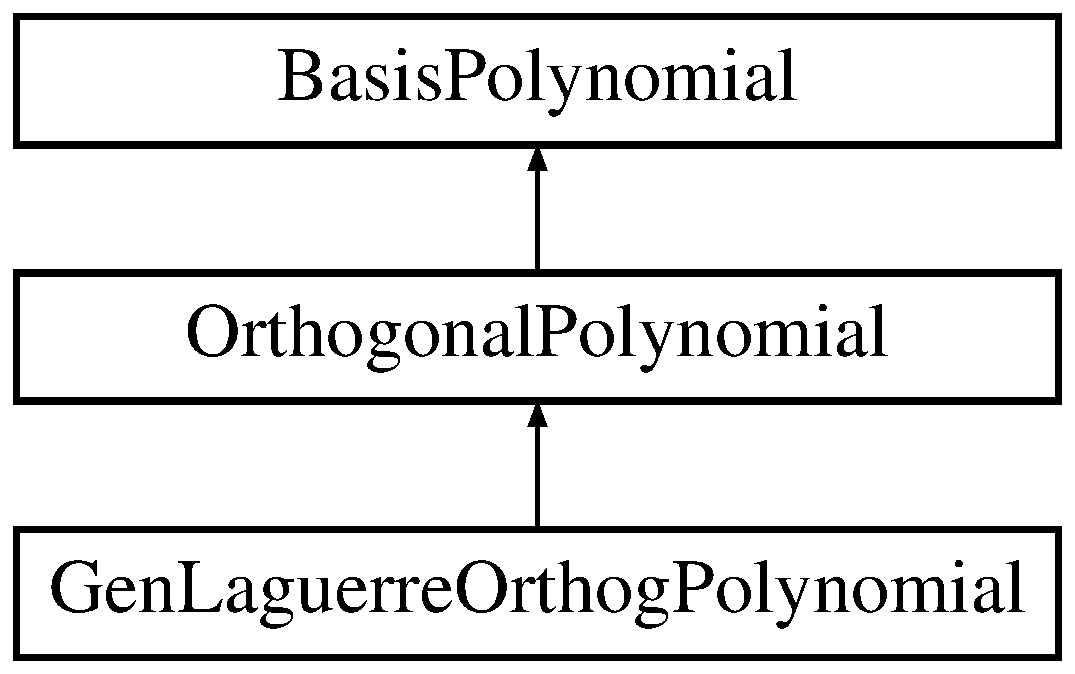
\includegraphics[height=3.000000cm]{classPecos_1_1GenLaguerreOrthogPolynomial}
\end{center}
\end{figure}
\subsection*{Public Member Functions}
\begin{DoxyCompactItemize}
\item 
\hyperlink{classPecos_1_1GenLaguerreOrthogPolynomial_a7a03d67906e4ef2afc868a23e93fd8b6}{Gen\+Laguerre\+Orthog\+Polynomial} ()\label{classPecos_1_1GenLaguerreOrthogPolynomial_a7a03d67906e4ef2afc868a23e93fd8b6}

\begin{DoxyCompactList}\small\item\em default constructor \end{DoxyCompactList}\item 
\hyperlink{classPecos_1_1GenLaguerreOrthogPolynomial_a2c97d43396fd28eb6040b943292959c0}{Gen\+Laguerre\+Orthog\+Polynomial} (Real \hyperlink{classPecos_1_1GenLaguerreOrthogPolynomial_aeeb4ce11a8d413209be1ec08eced8728}{alpha\+\_\+stat})\label{classPecos_1_1GenLaguerreOrthogPolynomial_a2c97d43396fd28eb6040b943292959c0}

\begin{DoxyCompactList}\small\item\em standard constructor \end{DoxyCompactList}\item 
\hyperlink{classPecos_1_1GenLaguerreOrthogPolynomial_a9d104277bc7d830f1ae5833c8809a7b0}{$\sim$\+Gen\+Laguerre\+Orthog\+Polynomial} ()\label{classPecos_1_1GenLaguerreOrthogPolynomial_a9d104277bc7d830f1ae5833c8809a7b0}

\begin{DoxyCompactList}\small\item\em destructor \end{DoxyCompactList}\item 
Real \hyperlink{classPecos_1_1GenLaguerreOrthogPolynomial_acc5475d6b992e443e3cce753a48cfc32}{weight\+\_\+factor} ()\label{classPecos_1_1GenLaguerreOrthogPolynomial_acc5475d6b992e443e3cce753a48cfc32}

\begin{DoxyCompactList}\small\item\em calculate and return wt\+Factor based on alpha\+Poly \end{DoxyCompactList}\end{DoxyCompactItemize}
\subsection*{Protected Member Functions}
\begin{DoxyCompactItemize}
\item 
Real \hyperlink{classPecos_1_1GenLaguerreOrthogPolynomial_a8792a858ac05a2158880e876f9da2019}{type1\+\_\+value} (Real x, unsigned short order)
\begin{DoxyCompactList}\small\item\em retrieve the value of the n\+\_\+th type 1 polynomial for a given parameter x using traditional characteristic polynomial formulation \end{DoxyCompactList}\item 
Real \hyperlink{classPecos_1_1GenLaguerreOrthogPolynomial_aac6751aa35bf5fcb42c520a322fc26dc}{type1\+\_\+gradient} (Real x, unsigned short order)
\begin{DoxyCompactList}\small\item\em retrieve the gradient of the n\+\_\+th type 1 polynomial for a given parameter x using traditional characteristic polynomial formulation \end{DoxyCompactList}\item 
Real \hyperlink{classPecos_1_1GenLaguerreOrthogPolynomial_ae957c8c2e7ea13728bafbad0c9b2996e}{type1\+\_\+hessian} (Real x, unsigned short order)
\begin{DoxyCompactList}\small\item\em retrieve the Hessian of the n\+\_\+th type 1 polynomial for a given parameter x using traditional characteristic polynomial formulation \end{DoxyCompactList}\item 
Real \hyperlink{classPecos_1_1GenLaguerreOrthogPolynomial_a77c0dbb874af1190d448d01da6efbe4e}{norm\+\_\+squared} (unsigned short order)
\begin{DoxyCompactList}\small\item\em returns the norm-\/squared of the n\+\_\+th order polynomial defined by the inner product $<$Poly\+\_\+n, Poly\+\_\+n$>$ = $\vert$$\vert$\+Poly\+\_\+n$\vert$$\vert$$^\wedge$2 \end{DoxyCompactList}\item 
const Real\+Array \& \hyperlink{classPecos_1_1GenLaguerreOrthogPolynomial_a10873b28f1284aff4ea214e00c4f86dd}{collocation\+\_\+points} (unsigned short order)
\begin{DoxyCompactList}\small\item\em return collocation points corresponding to orthogonal polynomial order n \end{DoxyCompactList}\item 
const Real\+Array \& \hyperlink{classPecos_1_1GenLaguerreOrthogPolynomial_aa010321cf47465dca5725fa15ba58bf6}{type1\+\_\+collocation\+\_\+weights} (unsigned short order)
\begin{DoxyCompactList}\small\item\em return the type 1 collocation weights corresponding to a point set of size order \end{DoxyCompactList}\item 
Real \hyperlink{classPecos_1_1GenLaguerreOrthogPolynomial_a997bdeddf670667c476513fcacc779ca}{alpha\+\_\+polynomial} () const \label{classPecos_1_1GenLaguerreOrthogPolynomial_a997bdeddf670667c476513fcacc779ca}

\begin{DoxyCompactList}\small\item\em return alpha\+Poly \end{DoxyCompactList}\item 
void \hyperlink{classPecos_1_1GenLaguerreOrthogPolynomial_aeeb4ce11a8d413209be1ec08eced8728}{alpha\+\_\+stat} (Real alpha)\label{classPecos_1_1GenLaguerreOrthogPolynomial_aeeb4ce11a8d413209be1ec08eced8728}

\begin{DoxyCompactList}\small\item\em set alpha\+Poly using the conversion alpha\+Poly = alpha\+\_\+stat-\/1. \end{DoxyCompactList}\item 
bool \hyperlink{classPecos_1_1GenLaguerreOrthogPolynomial_abc2afafc150f648667a41e0ce656b6da}{parameterized} () const \label{classPecos_1_1GenLaguerreOrthogPolynomial_abc2afafc150f648667a41e0ce656b6da}

\begin{DoxyCompactList}\small\item\em override default definition (false) since Gen\+Laguerre is parameterized \end{DoxyCompactList}\item 
Real \hyperlink{classPecos_1_1GenLaguerreOrthogPolynomial_a8c1e8d014e82efc5a1c20f973b5bc715}{length\+\_\+scale} () const 
\end{DoxyCompactItemize}
\subsection*{Private Attributes}
\begin{DoxyCompactItemize}
\item 
Real \hyperlink{classPecos_1_1GenLaguerreOrthogPolynomial_a11666846719189915a02ac6f1f96e393}{alpha\+Poly}\label{classPecos_1_1GenLaguerreOrthogPolynomial_a11666846719189915a02ac6f1f96e393}

\begin{DoxyCompactList}\small\item\em the alpha parameter for the generalized Laguerre polynomial as defined by Abramowitz and Stegun (differs from statistical P\+DF notation) \end{DoxyCompactList}\end{DoxyCompactItemize}
\subsection*{Additional Inherited Members}


\subsection{Detailed Description}
Derived orthogonal polynomial class for generalized Laguerre polynomials. 

The \hyperlink{classPecos_1_1GenLaguerreOrthogPolynomial}{Gen\+Laguerre\+Orthog\+Polynomial} class evaluates a univariate generalized/associated Laguerre polynomial L$^\wedge$(alpha)\+\_\+n of a particular order. These polynomials are orthogonal with respect to the weight function x$^\wedge$alpha exp(-\/x) when integrated over the support range of \mbox{[}0,+infinity\mbox{]}. This corresponds to the probability density function f(x) = x$^\wedge$alpha exp(-\/x) / Gamma(alpha+1) for the standard gamma distribution, although common statistical P\+DF parameter conventions (see, e.\+g., the uncertain variables section in the D\+A\+K\+O\+TA Reference Manual) and the Abramowitz and Stegun orthogonal polynomial parameter conventions require an offset conversion in this case (alpha\+\_\+poly = alpha\+\_\+stat -\/ 1 with the poly definition used in both cases above). It enables (mixed) multidimensional orthogonal polynomial basis functions within \hyperlink{classPecos_1_1OrthogPolyApproximation}{Orthog\+Poly\+Approximation}. A special case is the \hyperlink{classPecos_1_1LaguerreOrthogPolynomial}{Laguerre\+Orthog\+Polynomial} (implemented separately), for which alpha\+\_\+poly = 0 and weight function = exp(-\/x) (the standard exponential distribution). 

\subsection{Member Function Documentation}
\index{Pecos\+::\+Gen\+Laguerre\+Orthog\+Polynomial@{Pecos\+::\+Gen\+Laguerre\+Orthog\+Polynomial}!type1\+\_\+value@{type1\+\_\+value}}
\index{type1\+\_\+value@{type1\+\_\+value}!Pecos\+::\+Gen\+Laguerre\+Orthog\+Polynomial@{Pecos\+::\+Gen\+Laguerre\+Orthog\+Polynomial}}
\subsubsection[{\texorpdfstring{type1\+\_\+value(\+Real x, unsigned short order)}{type1_value(Real x, unsigned short order)}}]{\setlength{\rightskip}{0pt plus 5cm}Real type1\+\_\+value (
\begin{DoxyParamCaption}
\item[{Real}]{x, }
\item[{unsigned short}]{n}
\end{DoxyParamCaption}
)\hspace{0.3cm}{\ttfamily [protected]}, {\ttfamily [virtual]}}\label{classPecos_1_1GenLaguerreOrthogPolynomial_a8792a858ac05a2158880e876f9da2019}


retrieve the value of the n\+\_\+th type 1 polynomial for a given parameter x using traditional characteristic polynomial formulation 

For orthogonal polynomials, n specifies the order of the polynomial, whereas for interpolation polynomials, it identifies the interpolant for the n-\/th point. 

Reimplemented from \hyperlink{classPecos_1_1BasisPolynomial_a1fab871e99cec3a1933a2b1e9ed8a625}{Basis\+Polynomial}.



References Gen\+Laguerre\+Orthog\+Polynomial\+::alpha\+Poly.



Referenced by Gen\+Laguerre\+Orthog\+Polynomial\+::type1\+\_\+collocation\+\_\+weights(), and Gen\+Laguerre\+Orthog\+Polynomial\+::type1\+\_\+gradient().

\index{Pecos\+::\+Gen\+Laguerre\+Orthog\+Polynomial@{Pecos\+::\+Gen\+Laguerre\+Orthog\+Polynomial}!type1\+\_\+gradient@{type1\+\_\+gradient}}
\index{type1\+\_\+gradient@{type1\+\_\+gradient}!Pecos\+::\+Gen\+Laguerre\+Orthog\+Polynomial@{Pecos\+::\+Gen\+Laguerre\+Orthog\+Polynomial}}
\subsubsection[{\texorpdfstring{type1\+\_\+gradient(\+Real x, unsigned short order)}{type1_gradient(Real x, unsigned short order)}}]{\setlength{\rightskip}{0pt plus 5cm}Real type1\+\_\+gradient (
\begin{DoxyParamCaption}
\item[{Real}]{x, }
\item[{unsigned short}]{n}
\end{DoxyParamCaption}
)\hspace{0.3cm}{\ttfamily [protected]}, {\ttfamily [virtual]}}\label{classPecos_1_1GenLaguerreOrthogPolynomial_aac6751aa35bf5fcb42c520a322fc26dc}


retrieve the gradient of the n\+\_\+th type 1 polynomial for a given parameter x using traditional characteristic polynomial formulation 

For orthogonal polynomials, n specifies the order of the polynomial, whereas for interpolation polynomials, it identifies the interpolant for the n-\/th point. 

Reimplemented from \hyperlink{classPecos_1_1BasisPolynomial_a6f69ec84983f551e7e0e4a18b78b4498}{Basis\+Polynomial}.



References Gen\+Laguerre\+Orthog\+Polynomial\+::alpha\+Poly, and Gen\+Laguerre\+Orthog\+Polynomial\+::type1\+\_\+value().



Referenced by Gen\+Laguerre\+Orthog\+Polynomial\+::type1\+\_\+hessian().

\index{Pecos\+::\+Gen\+Laguerre\+Orthog\+Polynomial@{Pecos\+::\+Gen\+Laguerre\+Orthog\+Polynomial}!type1\+\_\+hessian@{type1\+\_\+hessian}}
\index{type1\+\_\+hessian@{type1\+\_\+hessian}!Pecos\+::\+Gen\+Laguerre\+Orthog\+Polynomial@{Pecos\+::\+Gen\+Laguerre\+Orthog\+Polynomial}}
\subsubsection[{\texorpdfstring{type1\+\_\+hessian(\+Real x, unsigned short order)}{type1_hessian(Real x, unsigned short order)}}]{\setlength{\rightskip}{0pt plus 5cm}Real type1\+\_\+hessian (
\begin{DoxyParamCaption}
\item[{Real}]{x, }
\item[{unsigned short}]{n}
\end{DoxyParamCaption}
)\hspace{0.3cm}{\ttfamily [protected]}, {\ttfamily [virtual]}}\label{classPecos_1_1GenLaguerreOrthogPolynomial_ae957c8c2e7ea13728bafbad0c9b2996e}


retrieve the Hessian of the n\+\_\+th type 1 polynomial for a given parameter x using traditional characteristic polynomial formulation 

For orthogonal polynomials, n specifies the order of the polynomial, whereas for interpolation polynomials, it identifies the interpolant for the n-\/th point. 

Reimplemented from \hyperlink{classPecos_1_1BasisPolynomial_a07d617dad8572dd606371e6c89ab6c35}{Basis\+Polynomial}.



References Gen\+Laguerre\+Orthog\+Polynomial\+::alpha\+Poly, and Gen\+Laguerre\+Orthog\+Polynomial\+::type1\+\_\+gradient().

\index{Pecos\+::\+Gen\+Laguerre\+Orthog\+Polynomial@{Pecos\+::\+Gen\+Laguerre\+Orthog\+Polynomial}!norm\+\_\+squared@{norm\+\_\+squared}}
\index{norm\+\_\+squared@{norm\+\_\+squared}!Pecos\+::\+Gen\+Laguerre\+Orthog\+Polynomial@{Pecos\+::\+Gen\+Laguerre\+Orthog\+Polynomial}}
\subsubsection[{\texorpdfstring{norm\+\_\+squared(unsigned short order)}{norm_squared(unsigned short order)}}]{\setlength{\rightskip}{0pt plus 5cm}Real norm\+\_\+squared (
\begin{DoxyParamCaption}
\item[{unsigned short}]{n}
\end{DoxyParamCaption}
)\hspace{0.3cm}{\ttfamily [protected]}, {\ttfamily [virtual]}}\label{classPecos_1_1GenLaguerreOrthogPolynomial_a77c0dbb874af1190d448d01da6efbe4e}


returns the norm-\/squared of the n\+\_\+th order polynomial defined by the inner product $<$Poly\+\_\+n, Poly\+\_\+n$>$ = $\vert$$\vert$\+Poly\+\_\+n$\vert$$\vert$$^\wedge$2 

This is defined only for orthogonal polynomials. 

Reimplemented from \hyperlink{classPecos_1_1BasisPolynomial_ab74383be309d74823f2e5e85dad739b2}{Basis\+Polynomial}.



References Gen\+Laguerre\+Orthog\+Polynomial\+::alpha\+Poly, Gen\+Laguerre\+Orthog\+Polynomial\+::collocation\+\_\+points(), Basis\+Polynomial\+::factorial(), and Basis\+Polynomial\+::pochhammer().

\index{Pecos\+::\+Gen\+Laguerre\+Orthog\+Polynomial@{Pecos\+::\+Gen\+Laguerre\+Orthog\+Polynomial}!collocation\+\_\+points@{collocation\+\_\+points}}
\index{collocation\+\_\+points@{collocation\+\_\+points}!Pecos\+::\+Gen\+Laguerre\+Orthog\+Polynomial@{Pecos\+::\+Gen\+Laguerre\+Orthog\+Polynomial}}
\subsubsection[{\texorpdfstring{collocation\+\_\+points(unsigned short order)}{collocation_points(unsigned short order)}}]{\setlength{\rightskip}{0pt plus 5cm}const Real\+Array \& collocation\+\_\+points (
\begin{DoxyParamCaption}
\item[{unsigned short}]{n}
\end{DoxyParamCaption}
)\hspace{0.3cm}{\ttfamily [protected]}, {\ttfamily [virtual]}}\label{classPecos_1_1GenLaguerreOrthogPolynomial_a10873b28f1284aff4ea214e00c4f86dd}


return collocation points corresponding to orthogonal polynomial order n 

This is defined for orthogonal and piecewise interpolation polynomials. 

Reimplemented from \hyperlink{classPecos_1_1BasisPolynomial_a0f96bd4e27ddc5c44117e7b68744b5a4}{Basis\+Polynomial}.



References Gen\+Laguerre\+Orthog\+Polynomial\+::alpha\+Poly, Orthogonal\+Polynomial\+::colloc\+Points, Orthogonal\+Polynomial\+::colloc\+Weights, Gen\+Laguerre\+Orthog\+Polynomial\+::type1\+\_\+collocation\+\_\+weights(), and Gen\+Laguerre\+Orthog\+Polynomial\+::weight\+\_\+factor().



Referenced by Gen\+Laguerre\+Orthog\+Polynomial\+::norm\+\_\+squared(), and Gen\+Laguerre\+Orthog\+Polynomial\+::type1\+\_\+collocation\+\_\+weights().

\index{Pecos\+::\+Gen\+Laguerre\+Orthog\+Polynomial@{Pecos\+::\+Gen\+Laguerre\+Orthog\+Polynomial}!type1\+\_\+collocation\+\_\+weights@{type1\+\_\+collocation\+\_\+weights}}
\index{type1\+\_\+collocation\+\_\+weights@{type1\+\_\+collocation\+\_\+weights}!Pecos\+::\+Gen\+Laguerre\+Orthog\+Polynomial@{Pecos\+::\+Gen\+Laguerre\+Orthog\+Polynomial}}
\subsubsection[{\texorpdfstring{type1\+\_\+collocation\+\_\+weights(unsigned short order)}{type1_collocation_weights(unsigned short order)}}]{\setlength{\rightskip}{0pt plus 5cm}const Real\+Array \& type1\+\_\+collocation\+\_\+weights (
\begin{DoxyParamCaption}
\item[{unsigned short}]{order}
\end{DoxyParamCaption}
)\hspace{0.3cm}{\ttfamily [protected]}, {\ttfamily [virtual]}}\label{classPecos_1_1GenLaguerreOrthogPolynomial_aa010321cf47465dca5725fa15ba58bf6}


return the type 1 collocation weights corresponding to a point set of size order 

This is defined for orthogonal and piecewise interpolation polynomials. 

Reimplemented from \hyperlink{classPecos_1_1BasisPolynomial_aa010321cf47465dca5725fa15ba58bf6}{Basis\+Polynomial}.



References Gen\+Laguerre\+Orthog\+Polynomial\+::alpha\+Poly, Gen\+Laguerre\+Orthog\+Polynomial\+::collocation\+\_\+points(), Orthogonal\+Polynomial\+::colloc\+Points, Orthogonal\+Polynomial\+::colloc\+Weights, Basis\+Polynomial\+::factorial(), Basis\+Polynomial\+::pochhammer(), Gen\+Laguerre\+Orthog\+Polynomial\+::type1\+\_\+value(), and Gen\+Laguerre\+Orthog\+Polynomial\+::weight\+\_\+factor().



Referenced by Gen\+Laguerre\+Orthog\+Polynomial\+::collocation\+\_\+points().

\index{Pecos\+::\+Gen\+Laguerre\+Orthog\+Polynomial@{Pecos\+::\+Gen\+Laguerre\+Orthog\+Polynomial}!length\+\_\+scale@{length\+\_\+scale}}
\index{length\+\_\+scale@{length\+\_\+scale}!Pecos\+::\+Gen\+Laguerre\+Orthog\+Polynomial@{Pecos\+::\+Gen\+Laguerre\+Orthog\+Polynomial}}
\subsubsection[{\texorpdfstring{length\+\_\+scale() const }{length_scale() const }}]{\setlength{\rightskip}{0pt plus 5cm}Real length\+\_\+scale (
\begin{DoxyParamCaption}
{}
\end{DoxyParamCaption}
) const\hspace{0.3cm}{\ttfamily [inline]}, {\ttfamily [protected]}, {\ttfamily [virtual]}}\label{classPecos_1_1GenLaguerreOrthogPolynomial_a8c1e8d014e82efc5a1c20f973b5bc715}
return max(mean,stdev) 

Reimplemented from \hyperlink{classPecos_1_1BasisPolynomial_a8c1e8d014e82efc5a1c20f973b5bc715}{Basis\+Polynomial}.



References Gen\+Laguerre\+Orthog\+Polynomial\+::alpha\+Poly.



The documentation for this class was generated from the following files\+:\begin{DoxyCompactItemize}
\item 
Gen\+Laguerre\+Orthog\+Polynomial.\+hpp\item 
Gen\+Laguerre\+Orthog\+Polynomial.\+cpp\end{DoxyCompactItemize}

\section{Geometric\+Random\+Variable Class Reference}
\label{classPecos_1_1GeometricRandomVariable}\index{Geometric\+Random\+Variable@{Geometric\+Random\+Variable}}


Derived random variable class for geometric random variables.  


Inheritance diagram for Geometric\+Random\+Variable\+:\begin{figure}[H]
\begin{center}
\leavevmode
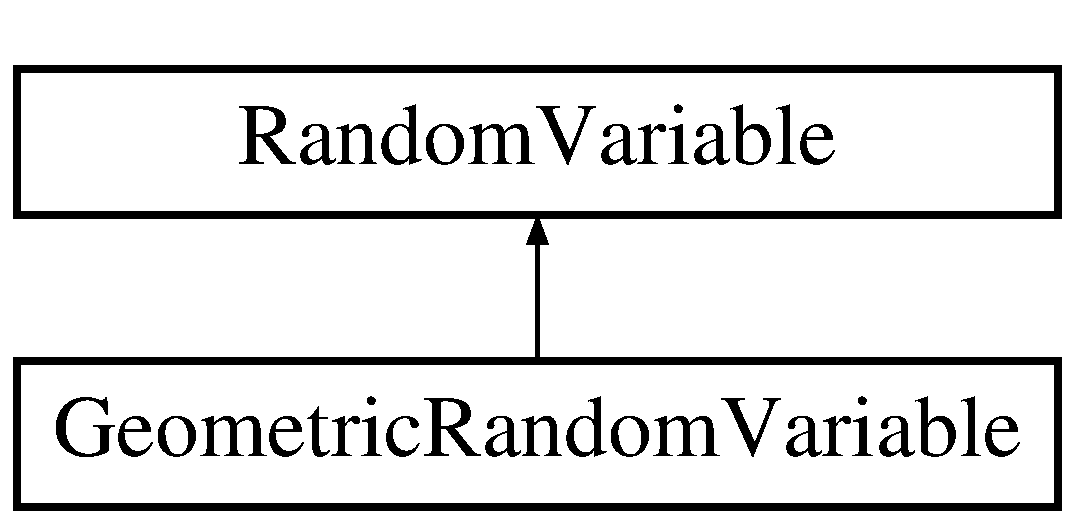
\includegraphics[height=2.000000cm]{classPecos_1_1GeometricRandomVariable}
\end{center}
\end{figure}
\subsection*{Public Member Functions}
\begin{DoxyCompactItemize}
\item 
\hyperlink{classPecos_1_1GeometricRandomVariable_a9319591af249156d43e3dfd81d8f382e}{Geometric\+Random\+Variable} ()\label{classPecos_1_1GeometricRandomVariable_a9319591af249156d43e3dfd81d8f382e}

\begin{DoxyCompactList}\small\item\em default constructor \end{DoxyCompactList}\item 
\hyperlink{classPecos_1_1GeometricRandomVariable_aab7bb48d5a2f0c0f2ae862a52998d9f0}{Geometric\+Random\+Variable} (Real prob\+\_\+per\+\_\+trial)\label{classPecos_1_1GeometricRandomVariable_aab7bb48d5a2f0c0f2ae862a52998d9f0}

\begin{DoxyCompactList}\small\item\em alternate constructor \end{DoxyCompactList}\item 
\hyperlink{classPecos_1_1GeometricRandomVariable_a4ce2a22a345a42afe8a9a609bf10c1d5}{$\sim$\+Geometric\+Random\+Variable} ()\label{classPecos_1_1GeometricRandomVariable_a4ce2a22a345a42afe8a9a609bf10c1d5}

\begin{DoxyCompactList}\small\item\em destructor \end{DoxyCompactList}\item 
Real \hyperlink{classPecos_1_1GeometricRandomVariable_addd564e7f4f314e12d38df74d845f0d8}{cdf} (Real x) const \label{classPecos_1_1GeometricRandomVariable_addd564e7f4f314e12d38df74d845f0d8}

\begin{DoxyCompactList}\small\item\em return the cumulative distribution function value of the random variable at x \end{DoxyCompactList}\item 
Real \hyperlink{classPecos_1_1GeometricRandomVariable_a23c3b599e7e4788a9a5e9e93c3dbaf4d}{ccdf} (Real x) const \label{classPecos_1_1GeometricRandomVariable_a23c3b599e7e4788a9a5e9e93c3dbaf4d}

\begin{DoxyCompactList}\small\item\em return the complementary cumulative distribution function value of the random variable at x \end{DoxyCompactList}\item 
Real \hyperlink{classPecos_1_1GeometricRandomVariable_a918a1aac05ca349ea5313eebcba46c3e}{inverse\+\_\+cdf} (Real p\+\_\+cdf) const \label{classPecos_1_1GeometricRandomVariable_a918a1aac05ca349ea5313eebcba46c3e}

\begin{DoxyCompactList}\small\item\em return the x value corresponding to a cumulative probability \end{DoxyCompactList}\item 
Real \hyperlink{classPecos_1_1GeometricRandomVariable_afda003a1f59ff6930902cd5c8601f49b}{inverse\+\_\+ccdf} (Real p\+\_\+ccdf) const \label{classPecos_1_1GeometricRandomVariable_afda003a1f59ff6930902cd5c8601f49b}

\begin{DoxyCompactList}\small\item\em return the x value corresponding to a complementary cumulative probability \end{DoxyCompactList}\item 
Real \hyperlink{classPecos_1_1GeometricRandomVariable_a8ec69265f428e17c1707133cb137a819}{pdf} (Real x) const \label{classPecos_1_1GeometricRandomVariable_a8ec69265f428e17c1707133cb137a819}

\begin{DoxyCompactList}\small\item\em return the value of the random variable\textquotesingle{}s probability density function at x \end{DoxyCompactList}\item 
Real \hyperlink{classPecos_1_1GeometricRandomVariable_aa891dab1ae9a225f493e3a0e5032b778}{parameter} (short dist\+\_\+param) const \label{classPecos_1_1GeometricRandomVariable_aa891dab1ae9a225f493e3a0e5032b778}

\begin{DoxyCompactList}\small\item\em return the value of the named distribution parameter \end{DoxyCompactList}\item 
void \hyperlink{classPecos_1_1GeometricRandomVariable_ae8e123224f588aee676d5d56d5ca900d}{parameter} (short dist\+\_\+param, Real val)\label{classPecos_1_1GeometricRandomVariable_ae8e123224f588aee676d5d56d5ca900d}

\begin{DoxyCompactList}\small\item\em update the value of the named distribution parameter \end{DoxyCompactList}\item 
Real \hyperlink{classPecos_1_1GeometricRandomVariable_a962ffe5a3593be370d5c883365c060f4}{mean} () const \label{classPecos_1_1GeometricRandomVariable_a962ffe5a3593be370d5c883365c060f4}

\begin{DoxyCompactList}\small\item\em return the distribution mean \end{DoxyCompactList}\item 
Real \hyperlink{classPecos_1_1GeometricRandomVariable_ae1fff19ce29a79d657043a598523635d}{median} () const \label{classPecos_1_1GeometricRandomVariable_ae1fff19ce29a79d657043a598523635d}

\begin{DoxyCompactList}\small\item\em return the distribution mode \end{DoxyCompactList}\item 
Real \hyperlink{classPecos_1_1GeometricRandomVariable_a72d3d6926edd929cb3f8e12baa655f70}{mode} () const \label{classPecos_1_1GeometricRandomVariable_a72d3d6926edd929cb3f8e12baa655f70}

\begin{DoxyCompactList}\small\item\em return the distribution mode \end{DoxyCompactList}\item 
Real \hyperlink{classPecos_1_1GeometricRandomVariable_a6a4ed9624d511f8a4e4f509c82cb0706}{standard\+\_\+deviation} () const \label{classPecos_1_1GeometricRandomVariable_a6a4ed9624d511f8a4e4f509c82cb0706}

\begin{DoxyCompactList}\small\item\em return the distribution variance \end{DoxyCompactList}\item 
Real \hyperlink{classPecos_1_1GeometricRandomVariable_a4b8b05b2a9af92dad9cc304c2925a4eb}{variance} () const \label{classPecos_1_1GeometricRandomVariable_a4b8b05b2a9af92dad9cc304c2925a4eb}

\begin{DoxyCompactList}\small\item\em return the distribution variance \end{DoxyCompactList}\item 
Real\+Real\+Pair \hyperlink{classPecos_1_1GeometricRandomVariable_a4bdb95a8fa5fffaa0de5102f56963cf2}{bounds} () const \label{classPecos_1_1GeometricRandomVariable_a4bdb95a8fa5fffaa0de5102f56963cf2}

\begin{DoxyCompactList}\small\item\em return the distribution lower and upper bounds as a pair \end{DoxyCompactList}\item 
void {\bfseries update} (Real prob\+\_\+per\+\_\+trial)\label{classPecos_1_1GeometricRandomVariable_a4f30d171bfc33f654cb85d1c5f23046a}

\end{DoxyCompactItemize}
\subsection*{Static Public Member Functions}
\begin{DoxyCompactItemize}
\item 
static Real {\bfseries pdf} (Real x, Real prob\+\_\+per\+\_\+trial)\label{classPecos_1_1GeometricRandomVariable_af19596bc5d4af3dff550b05920ed1fdd}

\item 
static Real {\bfseries cdf} (Real x, Real prob\+\_\+per\+\_\+trial)\label{classPecos_1_1GeometricRandomVariable_a501fe299ab60ca83642d33ff53cefc03}

\item 
static void {\bfseries moments\+\_\+from\+\_\+params} (Real prob\+\_\+per\+\_\+trial, Real \&\hyperlink{classPecos_1_1GeometricRandomVariable_a962ffe5a3593be370d5c883365c060f4}{mean}, Real \&std\+\_\+dev)\label{classPecos_1_1GeometricRandomVariable_a88140ecd8934bf4807efbd1cab8958ee}

\end{DoxyCompactItemize}
\subsection*{Protected Member Functions}
\begin{DoxyCompactItemize}
\item 
void \hyperlink{classPecos_1_1GeometricRandomVariable_aaa6750cbee2245416a6eeeac58d4405a}{update\+\_\+boost} ()\label{classPecos_1_1GeometricRandomVariable_aaa6750cbee2245416a6eeeac58d4405a}

\begin{DoxyCompactList}\small\item\em create a new geometric\+Dist instance \end{DoxyCompactList}\end{DoxyCompactItemize}
\subsection*{Protected Attributes}
\begin{DoxyCompactItemize}
\item 
Real \hyperlink{classPecos_1_1GeometricRandomVariable_a034cce918fd6c1433e74212387527794}{prob\+Per\+Trial}\label{classPecos_1_1GeometricRandomVariable_a034cce918fd6c1433e74212387527794}

\begin{DoxyCompactList}\small\item\em p parameter of geometric random variable \end{DoxyCompactList}\item 
geometric\+\_\+dist $\ast$ \hyperlink{classPecos_1_1GeometricRandomVariable_ac420bfe9c236be76e49f0ba14bfe893c}{geometric\+Dist}\label{classPecos_1_1GeometricRandomVariable_ac420bfe9c236be76e49f0ba14bfe893c}

\begin{DoxyCompactList}\small\item\em pointer to the Boost geometric\+\_\+distribution instance \end{DoxyCompactList}\end{DoxyCompactItemize}


\subsection{Detailed Description}
Derived random variable class for geometric random variables. 

Manages the prob\+Per\+Trial parameter. The geometric distribution is a special case of the negative binomial distribution for num\+Trials = 1. 

The documentation for this class was generated from the following file\+:\begin{DoxyCompactItemize}
\item 
Geometric\+Random\+Variable.\+hpp\end{DoxyCompactItemize}

\section{Gumbel\+Random\+Variable Class Reference}
\label{classPecos_1_1GumbelRandomVariable}\index{Gumbel\+Random\+Variable@{Gumbel\+Random\+Variable}}


Derived random variable class for gumbel random variables.  


Inheritance diagram for Gumbel\+Random\+Variable\+:\begin{figure}[H]
\begin{center}
\leavevmode
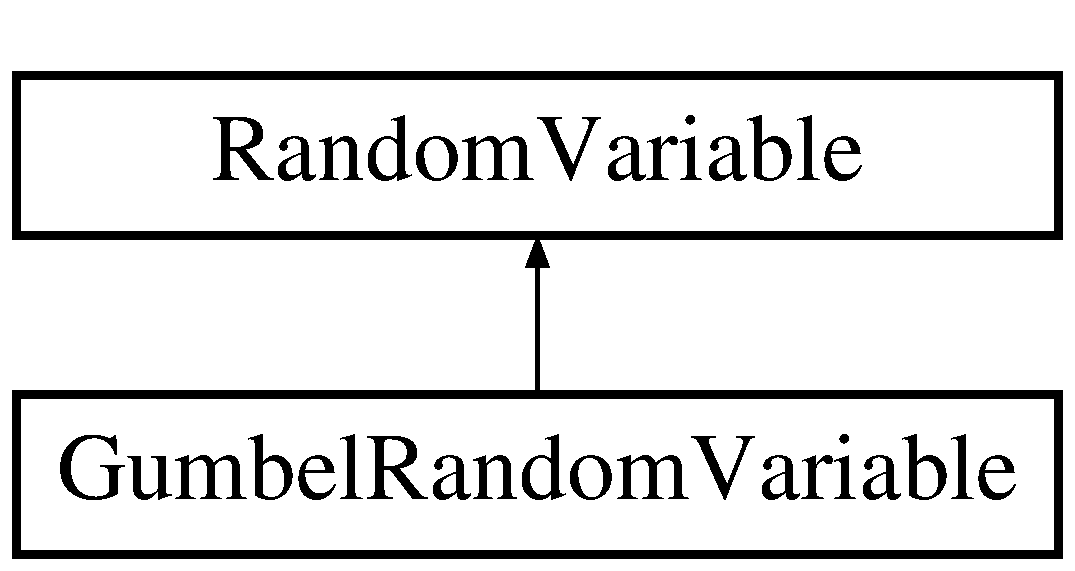
\includegraphics[height=2.000000cm]{classPecos_1_1GumbelRandomVariable}
\end{center}
\end{figure}
\subsection*{Public Member Functions}
\begin{DoxyCompactItemize}
\item 
\hyperlink{classPecos_1_1GumbelRandomVariable_a9b8e5c169d13dc96f25437fd74e11169}{Gumbel\+Random\+Variable} ()\label{classPecos_1_1GumbelRandomVariable_a9b8e5c169d13dc96f25437fd74e11169}

\begin{DoxyCompactList}\small\item\em default constructor \end{DoxyCompactList}\item 
\hyperlink{classPecos_1_1GumbelRandomVariable_a84bef444db8b649965f459585aa5aa87}{Gumbel\+Random\+Variable} (Real alpha, Real beta)\label{classPecos_1_1GumbelRandomVariable_a84bef444db8b649965f459585aa5aa87}

\begin{DoxyCompactList}\small\item\em alternate constructor \end{DoxyCompactList}\item 
\hyperlink{classPecos_1_1GumbelRandomVariable_af50fc451a40c1d048f25c2d278945d4d}{$\sim$\+Gumbel\+Random\+Variable} ()\label{classPecos_1_1GumbelRandomVariable_af50fc451a40c1d048f25c2d278945d4d}

\begin{DoxyCompactList}\small\item\em destructor \end{DoxyCompactList}\item 
Real \hyperlink{classPecos_1_1GumbelRandomVariable_addd564e7f4f314e12d38df74d845f0d8}{cdf} (Real x) const \label{classPecos_1_1GumbelRandomVariable_addd564e7f4f314e12d38df74d845f0d8}

\begin{DoxyCompactList}\small\item\em return the cumulative distribution function value of the random variable at x \end{DoxyCompactList}\item 
Real \hyperlink{classPecos_1_1GumbelRandomVariable_a23c3b599e7e4788a9a5e9e93c3dbaf4d}{ccdf} (Real x) const \label{classPecos_1_1GumbelRandomVariable_a23c3b599e7e4788a9a5e9e93c3dbaf4d}

\begin{DoxyCompactList}\small\item\em return the complementary cumulative distribution function value of the random variable at x \end{DoxyCompactList}\item 
Real \hyperlink{classPecos_1_1GumbelRandomVariable_a918a1aac05ca349ea5313eebcba46c3e}{inverse\+\_\+cdf} (Real p\+\_\+cdf) const \label{classPecos_1_1GumbelRandomVariable_a918a1aac05ca349ea5313eebcba46c3e}

\begin{DoxyCompactList}\small\item\em return the x value corresponding to a cumulative probability \end{DoxyCompactList}\item 
Real \hyperlink{classPecos_1_1GumbelRandomVariable_afda003a1f59ff6930902cd5c8601f49b}{inverse\+\_\+ccdf} (Real p\+\_\+ccdf) const \label{classPecos_1_1GumbelRandomVariable_afda003a1f59ff6930902cd5c8601f49b}

\begin{DoxyCompactList}\small\item\em return the x value corresponding to a complementary cumulative probability \end{DoxyCompactList}\item 
Real \hyperlink{classPecos_1_1GumbelRandomVariable_a8ec69265f428e17c1707133cb137a819}{pdf} (Real x) const \label{classPecos_1_1GumbelRandomVariable_a8ec69265f428e17c1707133cb137a819}

\begin{DoxyCompactList}\small\item\em return the value of the random variable\textquotesingle{}s probability density function at x \end{DoxyCompactList}\item 
Real \hyperlink{classPecos_1_1GumbelRandomVariable_aaa7ca3718abc034be7629af5594efca0}{pdf\+\_\+gradient} (Real x) const \label{classPecos_1_1GumbelRandomVariable_aaa7ca3718abc034be7629af5594efca0}

\begin{DoxyCompactList}\small\item\em return the gradient of the random variable\textquotesingle{}s probability density function at x \end{DoxyCompactList}\item 
Real \hyperlink{classPecos_1_1GumbelRandomVariable_a6e2b6b6f13eedb2eb1ef3bc455a06392}{log\+\_\+pdf} (Real x) const \label{classPecos_1_1GumbelRandomVariable_a6e2b6b6f13eedb2eb1ef3bc455a06392}

\begin{DoxyCompactList}\small\item\em return the value of the natural log of the random variable\textquotesingle{}s probability density function at x (useful for calculations of log density in Bayesian methods) \end{DoxyCompactList}\item 
Real \hyperlink{classPecos_1_1GumbelRandomVariable_aa891dab1ae9a225f493e3a0e5032b778}{parameter} (short dist\+\_\+param) const \label{classPecos_1_1GumbelRandomVariable_aa891dab1ae9a225f493e3a0e5032b778}

\begin{DoxyCompactList}\small\item\em return the value of the named distribution parameter \end{DoxyCompactList}\item 
void \hyperlink{classPecos_1_1GumbelRandomVariable_ae8e123224f588aee676d5d56d5ca900d}{parameter} (short dist\+\_\+param, Real val)\label{classPecos_1_1GumbelRandomVariable_ae8e123224f588aee676d5d56d5ca900d}

\begin{DoxyCompactList}\small\item\em update the value of the named distribution parameter \end{DoxyCompactList}\item 
Real \hyperlink{classPecos_1_1GumbelRandomVariable_a962ffe5a3593be370d5c883365c060f4}{mean} () const \label{classPecos_1_1GumbelRandomVariable_a962ffe5a3593be370d5c883365c060f4}

\begin{DoxyCompactList}\small\item\em return the distribution mean \end{DoxyCompactList}\item 
Real \hyperlink{classPecos_1_1GumbelRandomVariable_a72d3d6926edd929cb3f8e12baa655f70}{mode} () const \label{classPecos_1_1GumbelRandomVariable_a72d3d6926edd929cb3f8e12baa655f70}

\begin{DoxyCompactList}\small\item\em return the distribution mode \end{DoxyCompactList}\item 
Real \hyperlink{classPecos_1_1GumbelRandomVariable_a6a4ed9624d511f8a4e4f509c82cb0706}{standard\+\_\+deviation} () const \label{classPecos_1_1GumbelRandomVariable_a6a4ed9624d511f8a4e4f509c82cb0706}

\begin{DoxyCompactList}\small\item\em return the distribution variance \end{DoxyCompactList}\item 
Real \hyperlink{classPecos_1_1GumbelRandomVariable_a4b8b05b2a9af92dad9cc304c2925a4eb}{variance} () const \label{classPecos_1_1GumbelRandomVariable_a4b8b05b2a9af92dad9cc304c2925a4eb}

\begin{DoxyCompactList}\small\item\em return the distribution variance \end{DoxyCompactList}\item 
Real\+Real\+Pair \hyperlink{classPecos_1_1GumbelRandomVariable_a4bdb95a8fa5fffaa0de5102f56963cf2}{bounds} () const \label{classPecos_1_1GumbelRandomVariable_a4bdb95a8fa5fffaa0de5102f56963cf2}

\begin{DoxyCompactList}\small\item\em return the distribution lower and upper bounds as a pair \end{DoxyCompactList}\item 
Real \hyperlink{classPecos_1_1GumbelRandomVariable_a9ee48b3ca93459136b2e73f77873c4aa}{correlation\+\_\+warping\+\_\+factor} (const \hyperlink{classPecos_1_1RandomVariable}{Random\+Variable} \&rv, Real corr) const \label{classPecos_1_1GumbelRandomVariable_a9ee48b3ca93459136b2e73f77873c4aa}

\begin{DoxyCompactList}\small\item\em compute the warping factor for correlation between the current variable and the one passed in (used in \hyperlink{classPecos_1_1NatafTransformation}{Nataf\+Transformation}) \end{DoxyCompactList}\item 
Real \hyperlink{classPecos_1_1GumbelRandomVariable_af889af8adfb262c9b74f573b2a9ffc99}{dx\+\_\+ds} (short dist\+\_\+param, short u\+\_\+type, Real x, Real z) const 
\item 
Real \hyperlink{classPecos_1_1GumbelRandomVariable_af6b5fc528523180bed5fc3008dcea205}{dz\+\_\+ds\+\_\+factor} (short u\+\_\+type, Real x, Real z) const 
\item 
void {\bfseries update} (Real alpha, Real beta)\label{classPecos_1_1GumbelRandomVariable_aaa82eccfdca4d440a4e2d4a890b0d9ed}

\item 
Real \hyperlink{classPecos_1_1GumbelRandomVariable_a065b031fb613138ede20895562efc61f}{inverse\+\_\+log\+\_\+cdf} (Real log\+\_\+p) const \label{classPecos_1_1GumbelRandomVariable_a065b031fb613138ede20895562efc61f}

\begin{DoxyCompactList}\small\item\em inactive Z\+\_\+to\+\_\+X mapping option in \hyperlink{classPecos_1_1NatafTransformation}{Nataf\+Transformation} \end{DoxyCompactList}\end{DoxyCompactItemize}
\subsection*{Static Public Member Functions}
\begin{DoxyCompactItemize}
\item 
static Real {\bfseries pdf} (Real x, Real alpha, Real beta)\label{classPecos_1_1GumbelRandomVariable_a739d94cef9ee188f00056e229ca3fd95}

\item 
static Real {\bfseries cdf} (Real x, Real alpha, Real beta)\label{classPecos_1_1GumbelRandomVariable_a6ccc276bca2bfdfd6f320c65a6c8aaf7}

\item 
static void {\bfseries moments\+\_\+from\+\_\+params} (Real alpha, Real beta, Real \&\hyperlink{classPecos_1_1GumbelRandomVariable_a962ffe5a3593be370d5c883365c060f4}{mean}, Real \&std\+\_\+dev)\label{classPecos_1_1GumbelRandomVariable_af6459b831a8e62a41f7eab34d06edad8}

\end{DoxyCompactItemize}
\subsection*{Protected Attributes}
\begin{DoxyCompactItemize}
\item 
Real \hyperlink{classPecos_1_1GumbelRandomVariable_aa48da95b9214d9cf933e1d4625e32e84}{alpha\+Stat}\label{classPecos_1_1GumbelRandomVariable_aa48da95b9214d9cf933e1d4625e32e84}

\begin{DoxyCompactList}\small\item\em alpha parameter of gumbel random variable (inverse of scale) \end{DoxyCompactList}\item 
Real \hyperlink{classPecos_1_1GumbelRandomVariable_a838d220373c3360feec45e853b0daaac}{beta\+Stat}\label{classPecos_1_1GumbelRandomVariable_a838d220373c3360feec45e853b0daaac}

\begin{DoxyCompactList}\small\item\em beta parameter of gumbel random variable (location) \end{DoxyCompactList}\item 
Real\+Real\+Pair \hyperlink{classPecos_1_1GumbelRandomVariable_a019c4aba39508814cfdb412f6aef51c8}{exp\+Limits}\label{classPecos_1_1GumbelRandomVariable_a019c4aba39508814cfdb412f6aef51c8}

\begin{DoxyCompactList}\small\item\em overflow and underflow values for argument of std\+::exp \end{DoxyCompactList}\end{DoxyCompactItemize}
\subsection*{Additional Inherited Members}


\subsection{Detailed Description}
Derived random variable class for gumbel random variables. 

Manages alpha and beta parameters. See Haldar and Mahadevan, p. 90. 

\subsection{Member Function Documentation}
\index{Pecos\+::\+Gumbel\+Random\+Variable@{Pecos\+::\+Gumbel\+Random\+Variable}!dx\+\_\+ds@{dx\+\_\+ds}}
\index{dx\+\_\+ds@{dx\+\_\+ds}!Pecos\+::\+Gumbel\+Random\+Variable@{Pecos\+::\+Gumbel\+Random\+Variable}}
\subsubsection[{\texorpdfstring{dx\+\_\+ds(short dist\+\_\+param, short u\+\_\+type, Real x, Real z) const }{dx_ds(short dist_param, short u_type, Real x, Real z) const }}]{\setlength{\rightskip}{0pt plus 5cm}Real dx\+\_\+ds (
\begin{DoxyParamCaption}
\item[{short}]{dist\+\_\+param, }
\item[{short}]{u\+\_\+type, }
\item[{Real}]{x, }
\item[{Real}]{z}
\end{DoxyParamCaption}
) const\hspace{0.3cm}{\ttfamily [inline]}, {\ttfamily [virtual]}}\label{classPecos_1_1GumbelRandomVariable_af889af8adfb262c9b74f573b2a9ffc99}
dx/ds is derived by differentiating \hyperlink{classPecos_1_1NatafTransformation_a5feeecf846fc017c5a28eccb4e955dc1}{Nataf\+Transformation\+::trans\+\_\+\+Z\+\_\+to\+\_\+\+X()} with respect to distribution parameter s. dz/ds is zero if uncorrelated, while \hyperlink{classPecos_1_1GumbelRandomVariable_af6b5fc528523180bed5fc3008dcea205}{dz\+\_\+ds\+\_\+factor()} manages contributions in the correlated case. 

Reimplemented from \hyperlink{classPecos_1_1RandomVariable_af889af8adfb262c9b74f573b2a9ffc99}{Random\+Variable}.



References Gumbel\+Random\+Variable\+::alpha\+Stat, Gumbel\+Random\+Variable\+::beta\+Stat, and Gumbel\+Random\+Variable\+::dz\+\_\+ds\+\_\+factor().



Referenced by Gumbel\+Random\+Variable\+::correlation\+\_\+warping\+\_\+factor().

\index{Pecos\+::\+Gumbel\+Random\+Variable@{Pecos\+::\+Gumbel\+Random\+Variable}!dz\+\_\+ds\+\_\+factor@{dz\+\_\+ds\+\_\+factor}}
\index{dz\+\_\+ds\+\_\+factor@{dz\+\_\+ds\+\_\+factor}!Pecos\+::\+Gumbel\+Random\+Variable@{Pecos\+::\+Gumbel\+Random\+Variable}}
\subsubsection[{\texorpdfstring{dz\+\_\+ds\+\_\+factor(short u\+\_\+type, Real x, Real z) const }{dz_ds_factor(short u_type, Real x, Real z) const }}]{\setlength{\rightskip}{0pt plus 5cm}Real dz\+\_\+ds\+\_\+factor (
\begin{DoxyParamCaption}
\item[{short}]{u\+\_\+type, }
\item[{Real}]{x, }
\item[{Real}]{z}
\end{DoxyParamCaption}
) const\hspace{0.3cm}{\ttfamily [inline]}, {\ttfamily [virtual]}}\label{classPecos_1_1GumbelRandomVariable_af6b5fc528523180bed5fc3008dcea205}
dx/ds is derived by differentiating \hyperlink{classPecos_1_1NatafTransformation_a5feeecf846fc017c5a28eccb4e955dc1}{Nataf\+Transformation\+::trans\+\_\+\+Z\+\_\+to\+\_\+\+X()} with respect to distribution parameter s. For the uncorrelated case, u and z are constants. For the correlated case, u is a constant, but z(s) = L(s) u due to Nataf dependence on s and dz/ds = d\+L/ds u. 

Reimplemented from \hyperlink{classPecos_1_1RandomVariable_af6b5fc528523180bed5fc3008dcea205}{Random\+Variable}.



References Gumbel\+Random\+Variable\+::alpha\+Stat, Gumbel\+Random\+Variable\+::beta\+Stat, Gumbel\+Random\+Variable\+::cdf(), Gumbel\+Random\+Variable\+::mean(), Gumbel\+Random\+Variable\+::pdf(), Normal\+Random\+Variable\+::std\+\_\+cdf(), and Normal\+Random\+Variable\+::std\+\_\+pdf().



Referenced by Gumbel\+Random\+Variable\+::dx\+\_\+ds().



The documentation for this class was generated from the following file\+:\begin{DoxyCompactItemize}
\item 
Gumbel\+Random\+Variable.\+hpp\end{DoxyCompactItemize}

\section{Hahn\+Orthog\+Polynomial Class Reference}
\label{classPecos_1_1HahnOrthogPolynomial}\index{Hahn\+Orthog\+Polynomial@{Hahn\+Orthog\+Polynomial}}


Derived orthogonal polynomial class for Hahn polynomials.  


Inheritance diagram for Hahn\+Orthog\+Polynomial\+:\begin{figure}[H]
\begin{center}
\leavevmode
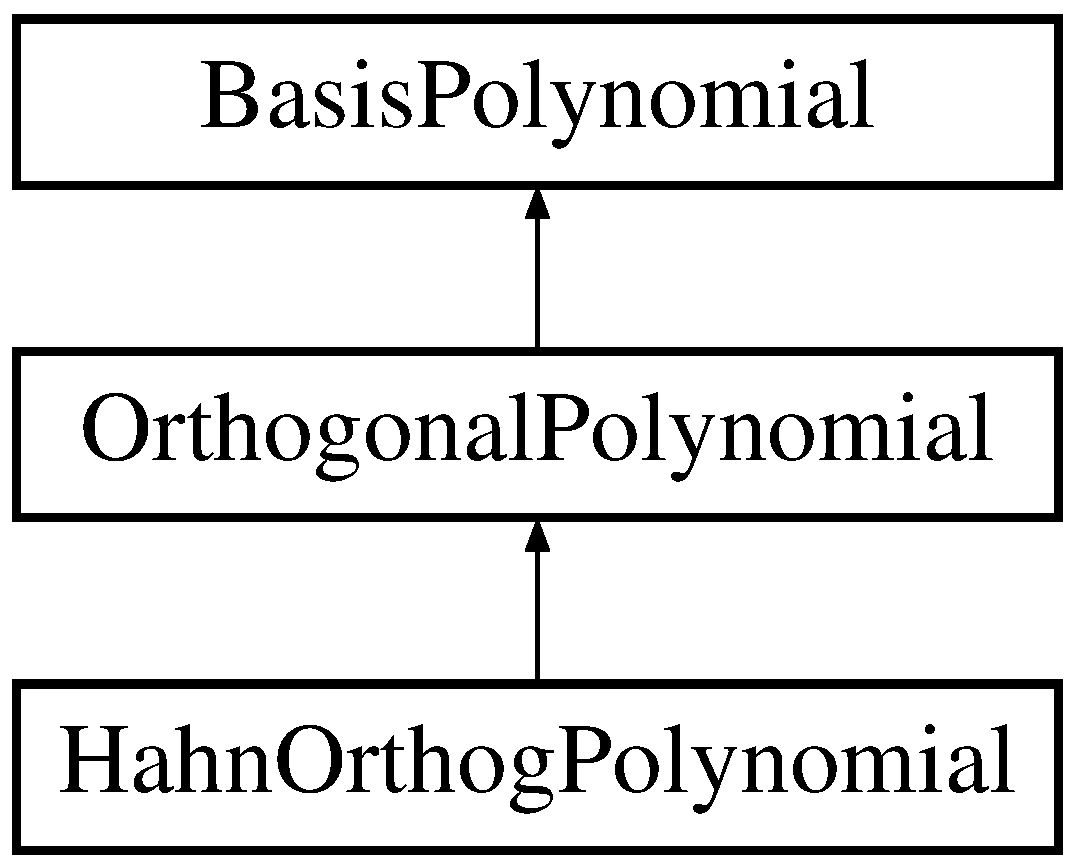
\includegraphics[height=3.000000cm]{classPecos_1_1HahnOrthogPolynomial}
\end{center}
\end{figure}
\subsection*{Public Member Functions}
\begin{DoxyCompactItemize}
\item 
\hyperlink{classPecos_1_1HahnOrthogPolynomial_a4c8c514febcc0b10dbc35aff617217b7}{Hahn\+Orthog\+Polynomial} ()\label{classPecos_1_1HahnOrthogPolynomial_a4c8c514febcc0b10dbc35aff617217b7}

\begin{DoxyCompactList}\small\item\em default constructor \end{DoxyCompactList}\item 
\hyperlink{classPecos_1_1HahnOrthogPolynomial_a165697a95cb62aba335fcae04c1bd5b8}{$\sim$\+Hahn\+Orthog\+Polynomial} ()\label{classPecos_1_1HahnOrthogPolynomial_a165697a95cb62aba335fcae04c1bd5b8}

\begin{DoxyCompactList}\small\item\em destructor \end{DoxyCompactList}\item 
Real \hyperlink{classPecos_1_1HahnOrthogPolynomial_a09f97f3d11434d8e62f63068ca8ce93f}{gamma\+\_\+polynomial} () const \label{classPecos_1_1HahnOrthogPolynomial_a09f97f3d11434d8e62f63068ca8ce93f}

\begin{DoxyCompactList}\small\item\em return gamma\+Poly \end{DoxyCompactList}\item 
void \hyperlink{classPecos_1_1HahnOrthogPolynomial_ad8e1174347b31063f1cc138be5da3199}{gamma\+\_\+stat} (Real gamma)\label{classPecos_1_1HahnOrthogPolynomial_ad8e1174347b31063f1cc138be5da3199}

\begin{DoxyCompactList}\small\item\em set gamma\+Stat (total population) \end{DoxyCompactList}\end{DoxyCompactItemize}
\subsection*{Protected Member Functions}
\begin{DoxyCompactItemize}
\item 
Real \hyperlink{classPecos_1_1HahnOrthogPolynomial_a8792a858ac05a2158880e876f9da2019}{type1\+\_\+value} (Real x, unsigned short order)
\begin{DoxyCompactList}\small\item\em retrieve the value of the n\+\_\+th type 1 polynomial for a given parameter x using traditional characteristic polynomial formulation \end{DoxyCompactList}\item 
Real \hyperlink{classPecos_1_1HahnOrthogPolynomial_a997bdeddf670667c476513fcacc779ca}{alpha\+\_\+polynomial} () const \label{classPecos_1_1HahnOrthogPolynomial_a997bdeddf670667c476513fcacc779ca}

\begin{DoxyCompactList}\small\item\em return alpha\+Poly \end{DoxyCompactList}\item 
Real \hyperlink{classPecos_1_1HahnOrthogPolynomial_a22bfc4209dec76716ef51648e945469a}{beta\+\_\+polynomial} () const \label{classPecos_1_1HahnOrthogPolynomial_a22bfc4209dec76716ef51648e945469a}

\begin{DoxyCompactList}\small\item\em return beta\+Poly \end{DoxyCompactList}\item 
void \hyperlink{classPecos_1_1HahnOrthogPolynomial_aeeb4ce11a8d413209be1ec08eced8728}{alpha\+\_\+stat} (Real alpha)\label{classPecos_1_1HahnOrthogPolynomial_aeeb4ce11a8d413209be1ec08eced8728}

\begin{DoxyCompactList}\small\item\em set alpha\+Stat (selected population) \end{DoxyCompactList}\item 
void \hyperlink{classPecos_1_1HahnOrthogPolynomial_a7f9584e538ee1574bd4d8d1afb622ed6}{beta\+\_\+stat} (Real beta)\label{classPecos_1_1HahnOrthogPolynomial_a7f9584e538ee1574bd4d8d1afb622ed6}

\begin{DoxyCompactList}\small\item\em set beta\+Stat (num draws) \end{DoxyCompactList}\end{DoxyCompactItemize}
\subsection*{Private Attributes}
\begin{DoxyCompactItemize}
\item 
Real \hyperlink{classPecos_1_1HahnOrthogPolynomial_a11666846719189915a02ac6f1f96e393}{alpha\+Poly}\label{classPecos_1_1HahnOrthogPolynomial_a11666846719189915a02ac6f1f96e393}

\begin{DoxyCompactList}\small\item\em the hypergeometric alpha parameter \end{DoxyCompactList}\item 
Real \hyperlink{classPecos_1_1HahnOrthogPolynomial_a96c0b0201ca445f95be14ec035b595cb}{beta\+Poly}\label{classPecos_1_1HahnOrthogPolynomial_a96c0b0201ca445f95be14ec035b595cb}

\begin{DoxyCompactList}\small\item\em the hypergeometric beta parameter \end{DoxyCompactList}\item 
Real \hyperlink{classPecos_1_1HahnOrthogPolynomial_aab2965f5a9b7c56742b552acb9f458b0}{gamma\+Poly}\label{classPecos_1_1HahnOrthogPolynomial_aab2965f5a9b7c56742b552acb9f458b0}

\begin{DoxyCompactList}\small\item\em the number of discrete points on which to base the polynomial \end{DoxyCompactList}\end{DoxyCompactItemize}
\subsection*{Additional Inherited Members}


\subsection{Detailed Description}
Derived orthogonal polynomial class for Hahn polynomials. 

The \hyperlink{classPecos_1_1HahnOrthogPolynomial}{Hahn\+Orthog\+Polynomial} class evaluates a univariate Hahn polynomial Q$^\wedge$(alpha,beta,N)\+\_\+n of a particular order. These polynomials are orthogonal with respect to the weight function

(K choose k)(N-\/K choose n-\/k)/( N choose n).

This corresponds to the hypergeometric probability mass function, which describes the probability of k successes in n draws, without replacement, from a finite population of size N that contains exactly K successes. See appendix in Xiu \& Karniadakis, Siam J. Sci. Comp., v24, n2, pp. 619-\/644, 2002 for more details. 

\subsection{Member Function Documentation}
\index{Pecos\+::\+Hahn\+Orthog\+Polynomial@{Pecos\+::\+Hahn\+Orthog\+Polynomial}!type1\+\_\+value@{type1\+\_\+value}}
\index{type1\+\_\+value@{type1\+\_\+value}!Pecos\+::\+Hahn\+Orthog\+Polynomial@{Pecos\+::\+Hahn\+Orthog\+Polynomial}}
\subsubsection[{\texorpdfstring{type1\+\_\+value(\+Real x, unsigned short order)}{type1_value(Real x, unsigned short order)}}]{\setlength{\rightskip}{0pt plus 5cm}Real type1\+\_\+value (
\begin{DoxyParamCaption}
\item[{Real}]{x, }
\item[{unsigned short}]{n}
\end{DoxyParamCaption}
)\hspace{0.3cm}{\ttfamily [protected]}, {\ttfamily [virtual]}}\label{classPecos_1_1HahnOrthogPolynomial_a8792a858ac05a2158880e876f9da2019}


retrieve the value of the n\+\_\+th type 1 polynomial for a given parameter x using traditional characteristic polynomial formulation 

For orthogonal polynomials, n specifies the order of the polynomial, whereas for interpolation polynomials, it identifies the interpolant for the n-\/th point. 

Reimplemented from \hyperlink{classPecos_1_1BasisPolynomial_a1fab871e99cec3a1933a2b1e9ed8a625}{Basis\+Polynomial}.



References Hahn\+Orthog\+Polynomial\+::alpha\+Poly, Hahn\+Orthog\+Polynomial\+::beta\+Poly, and Hahn\+Orthog\+Polynomial\+::gamma\+Poly.



The documentation for this class was generated from the following files\+:\begin{DoxyCompactItemize}
\item 
Hahn\+Orthog\+Polynomial.\+hpp\item 
Hahn\+Orthog\+Polynomial.\+cpp\end{DoxyCompactItemize}

\section{Hermite\+Interp\+Polynomial Class Reference}
\label{classPecos_1_1HermiteInterpPolynomial}\index{Hermite\+Interp\+Polynomial@{Hermite\+Interp\+Polynomial}}


Derived basis polynomial class for 1-\/D Hermite interpolation polynomials.  


Inheritance diagram for Hermite\+Interp\+Polynomial\+:\begin{figure}[H]
\begin{center}
\leavevmode
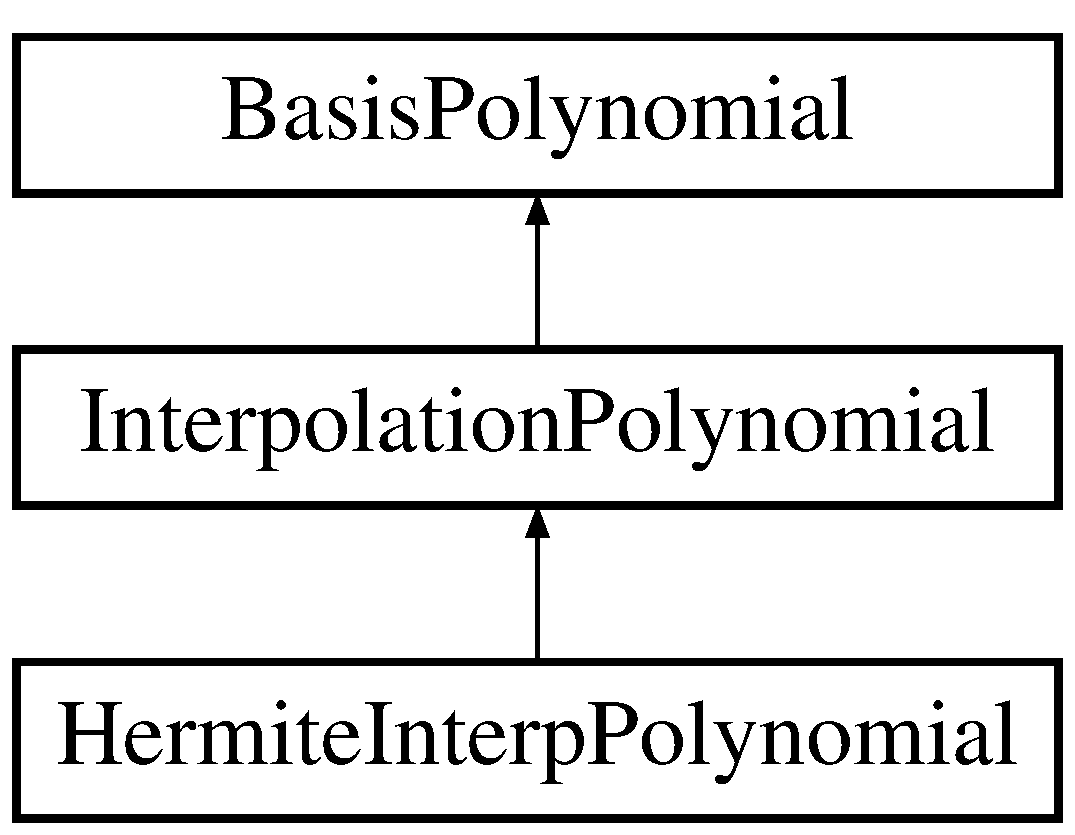
\includegraphics[height=3.000000cm]{classPecos_1_1HermiteInterpPolynomial}
\end{center}
\end{figure}
\subsection*{Public Member Functions}
\begin{DoxyCompactItemize}
\item 
\hyperlink{classPecos_1_1HermiteInterpPolynomial_ae13b0c3cd4bfb21c1e46fcd1deef7752}{Hermite\+Interp\+Polynomial} ()\label{classPecos_1_1HermiteInterpPolynomial_ae13b0c3cd4bfb21c1e46fcd1deef7752}

\begin{DoxyCompactList}\small\item\em default constructor \end{DoxyCompactList}\item 
\hyperlink{classPecos_1_1HermiteInterpPolynomial_aee3ed983c4e1ada90870429465dfdd3f}{Hermite\+Interp\+Polynomial} (short colloc\+\_\+rule)\label{classPecos_1_1HermiteInterpPolynomial_aee3ed983c4e1ada90870429465dfdd3f}

\begin{DoxyCompactList}\small\item\em constructor with collocation rule \end{DoxyCompactList}\item 
\hyperlink{classPecos_1_1HermiteInterpPolynomial_a3c90ca2245416714d418763bfaab1464}{Hermite\+Interp\+Polynomial} (const Real\+Array \&interp\+\_\+pts)\label{classPecos_1_1HermiteInterpPolynomial_a3c90ca2245416714d418763bfaab1464}

\begin{DoxyCompactList}\small\item\em constructor with set of interpolation points \end{DoxyCompactList}\item 
\hyperlink{classPecos_1_1HermiteInterpPolynomial_aa5e6863d8ffc9bca8b5fbd2babff8426}{$\sim$\+Hermite\+Interp\+Polynomial} ()\label{classPecos_1_1HermiteInterpPolynomial_aa5e6863d8ffc9bca8b5fbd2babff8426}

\begin{DoxyCompactList}\small\item\em destructor \end{DoxyCompactList}\end{DoxyCompactItemize}
\subsection*{Protected Member Functions}
\begin{DoxyCompactItemize}
\item 
void \hyperlink{classPecos_1_1HermiteInterpPolynomial_a9a5fd3dc945d15c8423dc66dcd137b4f}{precompute\+\_\+data} ()
\item 
Real \hyperlink{classPecos_1_1HermiteInterpPolynomial_abb79c6ea3bd58a7ca9c4b3bfdd85be9c}{type1\+\_\+value} (Real x, unsigned short i)
\item 
Real \hyperlink{classPecos_1_1HermiteInterpPolynomial_a49797f1037329fbe0a40f13dc23149e1}{type2\+\_\+value} (Real x, unsigned short i)
\item 
Real \hyperlink{classPecos_1_1HermiteInterpPolynomial_a005465761c081a210eef9879ec5686f8}{type1\+\_\+gradient} (Real x, unsigned short i)
\item 
Real \hyperlink{classPecos_1_1HermiteInterpPolynomial_a069b51a84ab3c4a6e635e07b3c8dcfe7}{type2\+\_\+gradient} (Real x, unsigned short i)
\item 
const Real\+Array \& \hyperlink{classPecos_1_1HermiteInterpPolynomial_a10873b28f1284aff4ea214e00c4f86dd}{collocation\+\_\+points} (unsigned short order)
\begin{DoxyCompactList}\small\item\em return collocation points corresponding to orthogonal polynomial order n \end{DoxyCompactList}\item 
const Real\+Array \& \hyperlink{classPecos_1_1HermiteInterpPolynomial_aa010321cf47465dca5725fa15ba58bf6}{type1\+\_\+collocation\+\_\+weights} (unsigned short order)
\begin{DoxyCompactList}\small\item\em return the type 1 collocation weights corresponding to a point set of size order \end{DoxyCompactList}\item 
const Real\+Array \& \hyperlink{classPecos_1_1HermiteInterpPolynomial_a8bc6cc516ab2bccbbdca6e904dc5a10f}{type2\+\_\+collocation\+\_\+weights} (unsigned short order)
\begin{DoxyCompactList}\small\item\em return the type 2 collocation weights corresponding to a point set of size order \end{DoxyCompactList}\item 
void \hyperlink{classPecos_1_1HermiteInterpPolynomial_addd13d4093ce8cbf2d22c47a47aff610}{collocation\+\_\+rule} (short rule)\label{classPecos_1_1HermiteInterpPolynomial_addd13d4093ce8cbf2d22c47a47aff610}

\begin{DoxyCompactList}\small\item\em set \hyperlink{classPecos_1_1OrthogonalPolynomial_abcc1d84cc8e8c8b5a66f720067039f2e}{Orthogonal\+Polynomial\+::colloc\+Rule} \end{DoxyCompactList}\item 
short \hyperlink{classPecos_1_1HermiteInterpPolynomial_a2e390f265fcc800348dc816d6cc37f86}{collocation\+\_\+rule} () const \label{classPecos_1_1HermiteInterpPolynomial_a2e390f265fcc800348dc816d6cc37f86}

\begin{DoxyCompactList}\small\item\em get \hyperlink{classPecos_1_1OrthogonalPolynomial_abcc1d84cc8e8c8b5a66f720067039f2e}{Orthogonal\+Polynomial\+::colloc\+Rule} \end{DoxyCompactList}\end{DoxyCompactItemize}
\subsection*{Private Attributes}
\begin{DoxyCompactItemize}
\item 
short \hyperlink{classPecos_1_1HermiteInterpPolynomial_abcc1d84cc8e8c8b5a66f720067039f2e}{colloc\+Rule}\label{classPecos_1_1HermiteInterpPolynomial_abcc1d84cc8e8c8b5a66f720067039f2e}

\begin{DoxyCompactList}\small\item\em name of uniform collocation rule\+: G\+A\+U\+S\+S\+\_\+\+P\+A\+T\+T\+E\+R\+S\+ON, C\+L\+E\+N\+S\+H\+A\+W\+\_\+\+C\+U\+R\+T\+IS, F\+E\+J\+E\+R2, or G\+A\+U\+S\+S\+\_\+\+L\+E\+G\+E\+N\+D\+RE \end{DoxyCompactList}\item 
Real\+Array \hyperlink{classPecos_1_1HermiteInterpPolynomial_a142635e1a0334e06cc17969f45121833}{type1\+Interp\+Wts}\label{classPecos_1_1HermiteInterpPolynomial_a142635e1a0334e06cc17969f45121833}

\begin{DoxyCompactList}\small\item\em set of 1-\/D weights for interpolation of values \end{DoxyCompactList}\item 
Real\+Array \hyperlink{classPecos_1_1HermiteInterpPolynomial_ae041c3717fb8258280964d7a37b2378c}{type2\+Interp\+Wts}\label{classPecos_1_1HermiteInterpPolynomial_ae041c3717fb8258280964d7a37b2378c}

\begin{DoxyCompactList}\small\item\em set of 1-\/D\mbox{]} weights for interpolation of gradients \end{DoxyCompactList}\item 
Real\+Array \hyperlink{classPecos_1_1HermiteInterpPolynomial_a7f82b2b501204c95f0e38508b8e9c2e8}{x\+Val\+Diff\+Tab}\label{classPecos_1_1HermiteInterpPolynomial_a7f82b2b501204c95f0e38508b8e9c2e8}

\begin{DoxyCompactList}\small\item\em pre-\/computed divided difference table for input used in type1/2 value calculation \end{DoxyCompactList}\item 
Real\+Array \hyperlink{classPecos_1_1HermiteInterpPolynomial_a4bf03d251b9dfca347e39d2aaf74e0e9}{x\+Grad\+Diff\+Tab}\label{classPecos_1_1HermiteInterpPolynomial_a4bf03d251b9dfca347e39d2aaf74e0e9}

\begin{DoxyCompactList}\small\item\em pre-\/computed divided difference table for input used in type1/2 gradient calculation \end{DoxyCompactList}\item 
Real2\+D\+Array \hyperlink{classPecos_1_1HermiteInterpPolynomial_a1a81078384a8ade468939ac1f4dffd00}{y\+T1\+Val\+Diff\+Tab}\label{classPecos_1_1HermiteInterpPolynomial_a1a81078384a8ade468939ac1f4dffd00}

\begin{DoxyCompactList}\small\item\em pre-\/computed divided difference table for output used in type1 value calculation \end{DoxyCompactList}\item 
Real2\+D\+Array \hyperlink{classPecos_1_1HermiteInterpPolynomial_a6941217fd7ac71c812db0263c3e11672}{y\+T1\+Grad\+Diff\+Tab}\label{classPecos_1_1HermiteInterpPolynomial_a6941217fd7ac71c812db0263c3e11672}

\begin{DoxyCompactList}\small\item\em pre-\/computed divided difference table for output used in type1 gradient calculation \end{DoxyCompactList}\item 
Real2\+D\+Array \hyperlink{classPecos_1_1HermiteInterpPolynomial_abbc8c4a533b3d75a2759cdceeb25c282}{y\+T2\+Val\+Diff\+Tab}\label{classPecos_1_1HermiteInterpPolynomial_abbc8c4a533b3d75a2759cdceeb25c282}

\begin{DoxyCompactList}\small\item\em pre-\/computed divided difference table for output used in type2 value calculation \end{DoxyCompactList}\item 
Real2\+D\+Array \hyperlink{classPecos_1_1HermiteInterpPolynomial_ac3605e3ae157a842df05bc016eeb777b}{y\+T2\+Grad\+Diff\+Tab}\label{classPecos_1_1HermiteInterpPolynomial_ac3605e3ae157a842df05bc016eeb777b}

\begin{DoxyCompactList}\small\item\em pre-\/computed divided difference table for output used in type2 gradient calculation \end{DoxyCompactList}\end{DoxyCompactItemize}
\subsection*{Additional Inherited Members}


\subsection{Detailed Description}
Derived basis polynomial class for 1-\/D Hermite interpolation polynomials. 

The \hyperlink{classPecos_1_1HermiteInterpPolynomial}{Hermite\+Interp\+Polynomial} class evaluates a univariate Hermite interpolation polynomial. The order of the polynomial is dictated by the number of interpolation points (order = N\+\_\+p -\/ 1). It enables multidimensional interpolants within \hyperlink{classPecos_1_1InterpPolyApproximation}{Interp\+Poly\+Approximation}. 

\subsection{Member Function Documentation}
\index{Pecos\+::\+Hermite\+Interp\+Polynomial@{Pecos\+::\+Hermite\+Interp\+Polynomial}!precompute\+\_\+data@{precompute\+\_\+data}}
\index{precompute\+\_\+data@{precompute\+\_\+data}!Pecos\+::\+Hermite\+Interp\+Polynomial@{Pecos\+::\+Hermite\+Interp\+Polynomial}}
\subsubsection[{\texorpdfstring{precompute\+\_\+data()}{precompute_data()}}]{\setlength{\rightskip}{0pt plus 5cm}void precompute\+\_\+data (
\begin{DoxyParamCaption}
{}
\end{DoxyParamCaption}
)\hspace{0.3cm}{\ttfamily [protected]}, {\ttfamily [virtual]}}\label{classPecos_1_1HermiteInterpPolynomial_a9a5fd3dc945d15c8423dc66dcd137b4f}
Pre-\/compute denominator products that are only a function of the interpolation points. 

Reimplemented from \hyperlink{classPecos_1_1InterpolationPolynomial_a9a5fd3dc945d15c8423dc66dcd137b4f}{Interpolation\+Polynomial}.



References Interpolation\+Polynomial\+::interp\+Pts, Hermite\+Interp\+Polynomial\+::type1\+\_\+gradient(), Hermite\+Interp\+Polynomial\+::type1\+\_\+value(), Hermite\+Interp\+Polynomial\+::type2\+\_\+gradient(), Hermite\+Interp\+Polynomial\+::type2\+\_\+value(), Hermite\+Interp\+Polynomial\+::x\+Grad\+Diff\+Tab, Hermite\+Interp\+Polynomial\+::x\+Val\+Diff\+Tab, Hermite\+Interp\+Polynomial\+::y\+T1\+Grad\+Diff\+Tab, Hermite\+Interp\+Polynomial\+::y\+T1\+Val\+Diff\+Tab, Hermite\+Interp\+Polynomial\+::y\+T2\+Grad\+Diff\+Tab, and Hermite\+Interp\+Polynomial\+::y\+T2\+Val\+Diff\+Tab.

\index{Pecos\+::\+Hermite\+Interp\+Polynomial@{Pecos\+::\+Hermite\+Interp\+Polynomial}!type1\+\_\+value@{type1\+\_\+value}}
\index{type1\+\_\+value@{type1\+\_\+value}!Pecos\+::\+Hermite\+Interp\+Polynomial@{Pecos\+::\+Hermite\+Interp\+Polynomial}}
\subsubsection[{\texorpdfstring{type1\+\_\+value(\+Real x, unsigned short i)}{type1_value(Real x, unsigned short i)}}]{\setlength{\rightskip}{0pt plus 5cm}Real type1\+\_\+value (
\begin{DoxyParamCaption}
\item[{Real}]{x, }
\item[{unsigned short}]{i}
\end{DoxyParamCaption}
)\hspace{0.3cm}{\ttfamily [protected]}, {\ttfamily [virtual]}}\label{classPecos_1_1HermiteInterpPolynomial_abb79c6ea3bd58a7ca9c4b3bfdd85be9c}
Compute value of the Hermite type 1 polynomial corresponding to interpolation point i. 

Reimplemented from \hyperlink{classPecos_1_1BasisPolynomial_a1fab871e99cec3a1933a2b1e9ed8a625}{Basis\+Polynomial}.



References Interpolation\+Polynomial\+::interp\+Pts, Hermite\+Interp\+Polynomial\+::x\+Grad\+Diff\+Tab, Hermite\+Interp\+Polynomial\+::x\+Val\+Diff\+Tab, Hermite\+Interp\+Polynomial\+::y\+T1\+Grad\+Diff\+Tab, and Hermite\+Interp\+Polynomial\+::y\+T1\+Val\+Diff\+Tab.



Referenced by Hermite\+Interp\+Polynomial\+::precompute\+\_\+data().

\index{Pecos\+::\+Hermite\+Interp\+Polynomial@{Pecos\+::\+Hermite\+Interp\+Polynomial}!type2\+\_\+value@{type2\+\_\+value}}
\index{type2\+\_\+value@{type2\+\_\+value}!Pecos\+::\+Hermite\+Interp\+Polynomial@{Pecos\+::\+Hermite\+Interp\+Polynomial}}
\subsubsection[{\texorpdfstring{type2\+\_\+value(\+Real x, unsigned short i)}{type2_value(Real x, unsigned short i)}}]{\setlength{\rightskip}{0pt plus 5cm}Real type2\+\_\+value (
\begin{DoxyParamCaption}
\item[{Real}]{x, }
\item[{unsigned short}]{i}
\end{DoxyParamCaption}
)\hspace{0.3cm}{\ttfamily [protected]}, {\ttfamily [virtual]}}\label{classPecos_1_1HermiteInterpPolynomial_a49797f1037329fbe0a40f13dc23149e1}
Compute value of the Hermite type 2 polynomial corresponding to interpolation point i. 

Reimplemented from \hyperlink{classPecos_1_1BasisPolynomial_aecd19f4bde44ba0cc371340405d81a18}{Basis\+Polynomial}.



References Interpolation\+Polynomial\+::interp\+Pts, Hermite\+Interp\+Polynomial\+::x\+Grad\+Diff\+Tab, Hermite\+Interp\+Polynomial\+::x\+Val\+Diff\+Tab, Hermite\+Interp\+Polynomial\+::y\+T2\+Grad\+Diff\+Tab, and Hermite\+Interp\+Polynomial\+::y\+T2\+Val\+Diff\+Tab.



Referenced by Hermite\+Interp\+Polynomial\+::precompute\+\_\+data().

\index{Pecos\+::\+Hermite\+Interp\+Polynomial@{Pecos\+::\+Hermite\+Interp\+Polynomial}!type1\+\_\+gradient@{type1\+\_\+gradient}}
\index{type1\+\_\+gradient@{type1\+\_\+gradient}!Pecos\+::\+Hermite\+Interp\+Polynomial@{Pecos\+::\+Hermite\+Interp\+Polynomial}}
\subsubsection[{\texorpdfstring{type1\+\_\+gradient(\+Real x, unsigned short i)}{type1_gradient(Real x, unsigned short i)}}]{\setlength{\rightskip}{0pt plus 5cm}Real type1\+\_\+gradient (
\begin{DoxyParamCaption}
\item[{Real}]{x, }
\item[{unsigned short}]{i}
\end{DoxyParamCaption}
)\hspace{0.3cm}{\ttfamily [protected]}, {\ttfamily [virtual]}}\label{classPecos_1_1HermiteInterpPolynomial_a005465761c081a210eef9879ec5686f8}
Compute derivative with respect to x of the Hermite type 1 polynomial corresponding to interpolation point i. 

Reimplemented from \hyperlink{classPecos_1_1BasisPolynomial_a6f69ec84983f551e7e0e4a18b78b4498}{Basis\+Polynomial}.



References Interpolation\+Polynomial\+::interp\+Pts, Hermite\+Interp\+Polynomial\+::x\+Grad\+Diff\+Tab, Hermite\+Interp\+Polynomial\+::x\+Val\+Diff\+Tab, Hermite\+Interp\+Polynomial\+::y\+T1\+Grad\+Diff\+Tab, and Hermite\+Interp\+Polynomial\+::y\+T1\+Val\+Diff\+Tab.



Referenced by Hermite\+Interp\+Polynomial\+::precompute\+\_\+data().

\index{Pecos\+::\+Hermite\+Interp\+Polynomial@{Pecos\+::\+Hermite\+Interp\+Polynomial}!type2\+\_\+gradient@{type2\+\_\+gradient}}
\index{type2\+\_\+gradient@{type2\+\_\+gradient}!Pecos\+::\+Hermite\+Interp\+Polynomial@{Pecos\+::\+Hermite\+Interp\+Polynomial}}
\subsubsection[{\texorpdfstring{type2\+\_\+gradient(\+Real x, unsigned short i)}{type2_gradient(Real x, unsigned short i)}}]{\setlength{\rightskip}{0pt plus 5cm}Real type2\+\_\+gradient (
\begin{DoxyParamCaption}
\item[{Real}]{x, }
\item[{unsigned short}]{i}
\end{DoxyParamCaption}
)\hspace{0.3cm}{\ttfamily [protected]}, {\ttfamily [virtual]}}\label{classPecos_1_1HermiteInterpPolynomial_a069b51a84ab3c4a6e635e07b3c8dcfe7}
Compute derivative with respect to x of the Hermite type 2 polynomial corresponding to interpolation point i. 

Reimplemented from \hyperlink{classPecos_1_1BasisPolynomial_a3a6b82f9baaa857ff03ea5a63ff48cc8}{Basis\+Polynomial}.



References Hermite\+Interp\+Polynomial\+::collocation\+\_\+points(), Interpolation\+Polynomial\+::interp\+Pts, Hermite\+Interp\+Polynomial\+::x\+Grad\+Diff\+Tab, Hermite\+Interp\+Polynomial\+::x\+Val\+Diff\+Tab, Hermite\+Interp\+Polynomial\+::y\+T2\+Grad\+Diff\+Tab, and Hermite\+Interp\+Polynomial\+::y\+T2\+Val\+Diff\+Tab.



Referenced by Hermite\+Interp\+Polynomial\+::precompute\+\_\+data().

\index{Pecos\+::\+Hermite\+Interp\+Polynomial@{Pecos\+::\+Hermite\+Interp\+Polynomial}!collocation\+\_\+points@{collocation\+\_\+points}}
\index{collocation\+\_\+points@{collocation\+\_\+points}!Pecos\+::\+Hermite\+Interp\+Polynomial@{Pecos\+::\+Hermite\+Interp\+Polynomial}}
\subsubsection[{\texorpdfstring{collocation\+\_\+points(unsigned short order)}{collocation_points(unsigned short order)}}]{\setlength{\rightskip}{0pt plus 5cm}const Real\+Array \& collocation\+\_\+points (
\begin{DoxyParamCaption}
\item[{unsigned short}]{n}
\end{DoxyParamCaption}
)\hspace{0.3cm}{\ttfamily [protected]}, {\ttfamily [virtual]}}\label{classPecos_1_1HermiteInterpPolynomial_a10873b28f1284aff4ea214e00c4f86dd}


return collocation points corresponding to orthogonal polynomial order n 

This is defined for orthogonal and piecewise interpolation polynomials. 

Reimplemented from \hyperlink{classPecos_1_1BasisPolynomial_a0f96bd4e27ddc5c44117e7b68744b5a4}{Basis\+Polynomial}.



References Hermite\+Interp\+Polynomial\+::colloc\+Rule, Interpolation\+Polynomial\+::interp\+Pts, and Hermite\+Interp\+Polynomial\+::type1\+\_\+collocation\+\_\+weights().



Referenced by Hermite\+Interp\+Polynomial\+::type1\+\_\+collocation\+\_\+weights(), Hermite\+Interp\+Polynomial\+::type2\+\_\+collocation\+\_\+weights(), and Hermite\+Interp\+Polynomial\+::type2\+\_\+gradient().

\index{Pecos\+::\+Hermite\+Interp\+Polynomial@{Pecos\+::\+Hermite\+Interp\+Polynomial}!type1\+\_\+collocation\+\_\+weights@{type1\+\_\+collocation\+\_\+weights}}
\index{type1\+\_\+collocation\+\_\+weights@{type1\+\_\+collocation\+\_\+weights}!Pecos\+::\+Hermite\+Interp\+Polynomial@{Pecos\+::\+Hermite\+Interp\+Polynomial}}
\subsubsection[{\texorpdfstring{type1\+\_\+collocation\+\_\+weights(unsigned short order)}{type1_collocation_weights(unsigned short order)}}]{\setlength{\rightskip}{0pt plus 5cm}const Real\+Array \& type1\+\_\+collocation\+\_\+weights (
\begin{DoxyParamCaption}
\item[{unsigned short}]{order}
\end{DoxyParamCaption}
)\hspace{0.3cm}{\ttfamily [protected]}, {\ttfamily [virtual]}}\label{classPecos_1_1HermiteInterpPolynomial_aa010321cf47465dca5725fa15ba58bf6}


return the type 1 collocation weights corresponding to a point set of size order 

This is defined for orthogonal and piecewise interpolation polynomials. 

Reimplemented from \hyperlink{classPecos_1_1BasisPolynomial_aa010321cf47465dca5725fa15ba58bf6}{Basis\+Polynomial}.



References Hermite\+Interp\+Polynomial\+::collocation\+\_\+points(), Interpolation\+Polynomial\+::interp\+Pts, Hermite\+Interp\+Polynomial\+::type1\+Interp\+Wts, Hermite\+Interp\+Polynomial\+::type2\+\_\+collocation\+\_\+weights(), Hermite\+Interp\+Polynomial\+::type2\+Interp\+Wts, and Basis\+Polynomial\+::wt\+Factor.



Referenced by Hermite\+Interp\+Polynomial\+::collocation\+\_\+points().

\index{Pecos\+::\+Hermite\+Interp\+Polynomial@{Pecos\+::\+Hermite\+Interp\+Polynomial}!type2\+\_\+collocation\+\_\+weights@{type2\+\_\+collocation\+\_\+weights}}
\index{type2\+\_\+collocation\+\_\+weights@{type2\+\_\+collocation\+\_\+weights}!Pecos\+::\+Hermite\+Interp\+Polynomial@{Pecos\+::\+Hermite\+Interp\+Polynomial}}
\subsubsection[{\texorpdfstring{type2\+\_\+collocation\+\_\+weights(unsigned short order)}{type2_collocation_weights(unsigned short order)}}]{\setlength{\rightskip}{0pt plus 5cm}const Real\+Array \& type2\+\_\+collocation\+\_\+weights (
\begin{DoxyParamCaption}
\item[{unsigned short}]{order}
\end{DoxyParamCaption}
)\hspace{0.3cm}{\ttfamily [protected]}, {\ttfamily [virtual]}}\label{classPecos_1_1HermiteInterpPolynomial_a8bc6cc516ab2bccbbdca6e904dc5a10f}


return the type 2 collocation weights corresponding to a point set of size order 

This is defined for piecewise interpolation polynomials. 

Reimplemented from \hyperlink{classPecos_1_1BasisPolynomial_a8bc6cc516ab2bccbbdca6e904dc5a10f}{Basis\+Polynomial}.



References Hermite\+Interp\+Polynomial\+::collocation\+\_\+points(), Interpolation\+Polynomial\+::interp\+Pts, Hermite\+Interp\+Polynomial\+::type1\+Interp\+Wts, Hermite\+Interp\+Polynomial\+::type2\+Interp\+Wts, and Basis\+Polynomial\+::wt\+Factor.



Referenced by Hermite\+Interp\+Polynomial\+::type1\+\_\+collocation\+\_\+weights().



The documentation for this class was generated from the following files\+:\begin{DoxyCompactItemize}
\item 
Hermite\+Interp\+Polynomial.\+hpp\item 
Hermite\+Interp\+Polynomial.\+cpp\end{DoxyCompactItemize}

\section{Hermite\+Orthog\+Polynomial Class Reference}
\label{classPecos_1_1HermiteOrthogPolynomial}\index{Hermite\+Orthog\+Polynomial@{Hermite\+Orthog\+Polynomial}}


Derived orthogonal polynomial class for Hermite polynomials.  


Inheritance diagram for Hermite\+Orthog\+Polynomial\+:\begin{figure}[H]
\begin{center}
\leavevmode
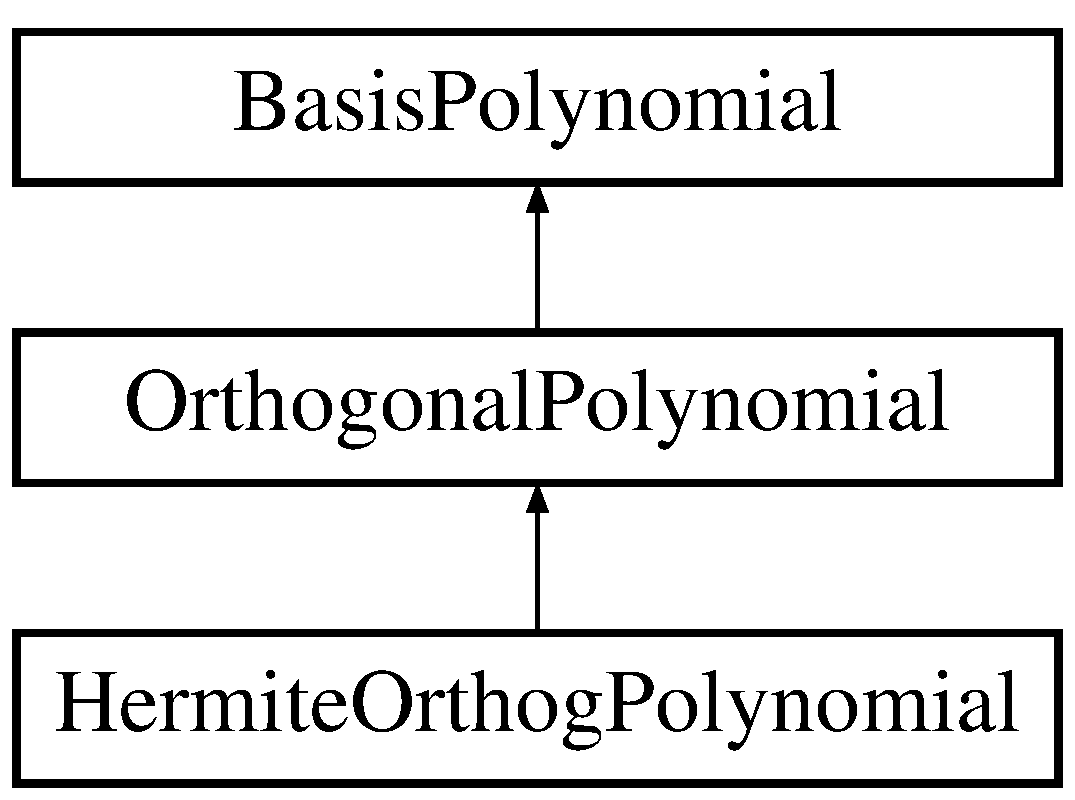
\includegraphics[height=3.000000cm]{classPecos_1_1HermiteOrthogPolynomial}
\end{center}
\end{figure}
\subsection*{Public Member Functions}
\begin{DoxyCompactItemize}
\item 
\hyperlink{classPecos_1_1HermiteOrthogPolynomial_a31e12af801682b17d3a4bfa2c9909a39}{Hermite\+Orthog\+Polynomial} (short colloc\+\_\+rule)\label{classPecos_1_1HermiteOrthogPolynomial_a31e12af801682b17d3a4bfa2c9909a39}

\begin{DoxyCompactList}\small\item\em extended constructor \end{DoxyCompactList}\item 
\hyperlink{classPecos_1_1HermiteOrthogPolynomial_ae2079621617f6eb4c03fbd90e4e3d2fa}{Hermite\+Orthog\+Polynomial} ()\label{classPecos_1_1HermiteOrthogPolynomial_ae2079621617f6eb4c03fbd90e4e3d2fa}

\begin{DoxyCompactList}\small\item\em default constructor \end{DoxyCompactList}\item 
\hyperlink{classPecos_1_1HermiteOrthogPolynomial_a7036e911ad89269a5f40157e0562de19}{$\sim$\+Hermite\+Orthog\+Polynomial} ()\label{classPecos_1_1HermiteOrthogPolynomial_a7036e911ad89269a5f40157e0562de19}

\begin{DoxyCompactList}\small\item\em destructor \end{DoxyCompactList}\end{DoxyCompactItemize}
\subsection*{Protected Member Functions}
\begin{DoxyCompactItemize}
\item 
Real \hyperlink{classPecos_1_1HermiteOrthogPolynomial_a8792a858ac05a2158880e876f9da2019}{type1\+\_\+value} (Real x, unsigned short order)
\begin{DoxyCompactList}\small\item\em retrieve the value of the n\+\_\+th type 1 polynomial for a given parameter x using traditional characteristic polynomial formulation \end{DoxyCompactList}\item 
Real \hyperlink{classPecos_1_1HermiteOrthogPolynomial_aac6751aa35bf5fcb42c520a322fc26dc}{type1\+\_\+gradient} (Real x, unsigned short order)
\begin{DoxyCompactList}\small\item\em retrieve the gradient of the n\+\_\+th type 1 polynomial for a given parameter x using traditional characteristic polynomial formulation \end{DoxyCompactList}\item 
Real \hyperlink{classPecos_1_1HermiteOrthogPolynomial_ae957c8c2e7ea13728bafbad0c9b2996e}{type1\+\_\+hessian} (Real x, unsigned short order)
\begin{DoxyCompactList}\small\item\em retrieve the Hessian of the n\+\_\+th type 1 polynomial for a given parameter x using traditional characteristic polynomial formulation \end{DoxyCompactList}\item 
Real \hyperlink{classPecos_1_1HermiteOrthogPolynomial_a77c0dbb874af1190d448d01da6efbe4e}{norm\+\_\+squared} (unsigned short order)
\begin{DoxyCompactList}\small\item\em returns the norm-\/squared of the n\+\_\+th order polynomial defined by the inner product $<$Poly\+\_\+n, Poly\+\_\+n$>$ = $\vert$$\vert$\+Poly\+\_\+n$\vert$$\vert$$^\wedge$2 \end{DoxyCompactList}\item 
const Real\+Array \& \hyperlink{classPecos_1_1HermiteOrthogPolynomial_a10873b28f1284aff4ea214e00c4f86dd}{collocation\+\_\+points} (unsigned short order)
\begin{DoxyCompactList}\small\item\em return collocation points corresponding to orthogonal polynomial order n \end{DoxyCompactList}\item 
const Real\+Array \& \hyperlink{classPecos_1_1HermiteOrthogPolynomial_aa010321cf47465dca5725fa15ba58bf6}{type1\+\_\+collocation\+\_\+weights} (unsigned short order)
\begin{DoxyCompactList}\small\item\em return the type 1 collocation weights corresponding to a point set of size order \end{DoxyCompactList}\item 
Real \hyperlink{classPecos_1_1HermiteOrthogPolynomial_a8c1e8d014e82efc5a1c20f973b5bc715}{length\+\_\+scale} () const 
\end{DoxyCompactItemize}
\subsection*{Additional Inherited Members}


\subsection{Detailed Description}
Derived orthogonal polynomial class for Hermite polynomials. 

The \hyperlink{classPecos_1_1HermiteOrthogPolynomial}{Hermite\+Orthog\+Polynomial} class evaluates a univariate Hermite polynomial of a particular order. It uses the \char`\"{}probabilist\textquotesingle{}s\char`\"{} formulation for which the polynomials are orthogonal with respect to the weight function 1/std\+::sqrt(2$\ast$\+P\+I) exp(-\/x$^\wedge$2/2) when integrated over the support range of \mbox{[}-\/infinity,+infinity\mbox{]}. It enables (mixed) multidimensional orthogonal polynomial basis functions within \hyperlink{classPecos_1_1OrthogPolyApproximation}{Orthog\+Poly\+Approximation}. 

\subsection{Member Function Documentation}
\index{Pecos\+::\+Hermite\+Orthog\+Polynomial@{Pecos\+::\+Hermite\+Orthog\+Polynomial}!type1\+\_\+value@{type1\+\_\+value}}
\index{type1\+\_\+value@{type1\+\_\+value}!Pecos\+::\+Hermite\+Orthog\+Polynomial@{Pecos\+::\+Hermite\+Orthog\+Polynomial}}
\subsubsection[{\texorpdfstring{type1\+\_\+value(\+Real x, unsigned short order)}{type1_value(Real x, unsigned short order)}}]{\setlength{\rightskip}{0pt plus 5cm}Real type1\+\_\+value (
\begin{DoxyParamCaption}
\item[{Real}]{x, }
\item[{unsigned short}]{n}
\end{DoxyParamCaption}
)\hspace{0.3cm}{\ttfamily [protected]}, {\ttfamily [virtual]}}\label{classPecos_1_1HermiteOrthogPolynomial_a8792a858ac05a2158880e876f9da2019}


retrieve the value of the n\+\_\+th type 1 polynomial for a given parameter x using traditional characteristic polynomial formulation 

For orthogonal polynomials, n specifies the order of the polynomial, whereas for interpolation polynomials, it identifies the interpolant for the n-\/th point. 

Reimplemented from \hyperlink{classPecos_1_1BasisPolynomial_a1fab871e99cec3a1933a2b1e9ed8a625}{Basis\+Polynomial}.



Referenced by Hermite\+Orthog\+Polynomial\+::type1\+\_\+collocation\+\_\+weights(), Hermite\+Orthog\+Polynomial\+::type1\+\_\+gradient(), and Hermite\+Orthog\+Polynomial\+::type1\+\_\+hessian().

\index{Pecos\+::\+Hermite\+Orthog\+Polynomial@{Pecos\+::\+Hermite\+Orthog\+Polynomial}!type1\+\_\+gradient@{type1\+\_\+gradient}}
\index{type1\+\_\+gradient@{type1\+\_\+gradient}!Pecos\+::\+Hermite\+Orthog\+Polynomial@{Pecos\+::\+Hermite\+Orthog\+Polynomial}}
\subsubsection[{\texorpdfstring{type1\+\_\+gradient(\+Real x, unsigned short order)}{type1_gradient(Real x, unsigned short order)}}]{\setlength{\rightskip}{0pt plus 5cm}Real type1\+\_\+gradient (
\begin{DoxyParamCaption}
\item[{Real}]{x, }
\item[{unsigned short}]{n}
\end{DoxyParamCaption}
)\hspace{0.3cm}{\ttfamily [protected]}, {\ttfamily [virtual]}}\label{classPecos_1_1HermiteOrthogPolynomial_aac6751aa35bf5fcb42c520a322fc26dc}


retrieve the gradient of the n\+\_\+th type 1 polynomial for a given parameter x using traditional characteristic polynomial formulation 

For orthogonal polynomials, n specifies the order of the polynomial, whereas for interpolation polynomials, it identifies the interpolant for the n-\/th point. 

Reimplemented from \hyperlink{classPecos_1_1BasisPolynomial_a6f69ec84983f551e7e0e4a18b78b4498}{Basis\+Polynomial}.



References Hermite\+Orthog\+Polynomial\+::type1\+\_\+value().

\index{Pecos\+::\+Hermite\+Orthog\+Polynomial@{Pecos\+::\+Hermite\+Orthog\+Polynomial}!type1\+\_\+hessian@{type1\+\_\+hessian}}
\index{type1\+\_\+hessian@{type1\+\_\+hessian}!Pecos\+::\+Hermite\+Orthog\+Polynomial@{Pecos\+::\+Hermite\+Orthog\+Polynomial}}
\subsubsection[{\texorpdfstring{type1\+\_\+hessian(\+Real x, unsigned short order)}{type1_hessian(Real x, unsigned short order)}}]{\setlength{\rightskip}{0pt plus 5cm}Real type1\+\_\+hessian (
\begin{DoxyParamCaption}
\item[{Real}]{x, }
\item[{unsigned short}]{n}
\end{DoxyParamCaption}
)\hspace{0.3cm}{\ttfamily [protected]}, {\ttfamily [virtual]}}\label{classPecos_1_1HermiteOrthogPolynomial_ae957c8c2e7ea13728bafbad0c9b2996e}


retrieve the Hessian of the n\+\_\+th type 1 polynomial for a given parameter x using traditional characteristic polynomial formulation 

For orthogonal polynomials, n specifies the order of the polynomial, whereas for interpolation polynomials, it identifies the interpolant for the n-\/th point. 

Reimplemented from \hyperlink{classPecos_1_1BasisPolynomial_a07d617dad8572dd606371e6c89ab6c35}{Basis\+Polynomial}.



References Hermite\+Orthog\+Polynomial\+::type1\+\_\+value().

\index{Pecos\+::\+Hermite\+Orthog\+Polynomial@{Pecos\+::\+Hermite\+Orthog\+Polynomial}!norm\+\_\+squared@{norm\+\_\+squared}}
\index{norm\+\_\+squared@{norm\+\_\+squared}!Pecos\+::\+Hermite\+Orthog\+Polynomial@{Pecos\+::\+Hermite\+Orthog\+Polynomial}}
\subsubsection[{\texorpdfstring{norm\+\_\+squared(unsigned short order)}{norm_squared(unsigned short order)}}]{\setlength{\rightskip}{0pt plus 5cm}Real norm\+\_\+squared (
\begin{DoxyParamCaption}
\item[{unsigned short}]{n}
\end{DoxyParamCaption}
)\hspace{0.3cm}{\ttfamily [protected]}, {\ttfamily [virtual]}}\label{classPecos_1_1HermiteOrthogPolynomial_a77c0dbb874af1190d448d01da6efbe4e}


returns the norm-\/squared of the n\+\_\+th order polynomial defined by the inner product $<$Poly\+\_\+n, Poly\+\_\+n$>$ = $\vert$$\vert$\+Poly\+\_\+n$\vert$$\vert$$^\wedge$2 

This is defined only for orthogonal polynomials. 

Reimplemented from \hyperlink{classPecos_1_1BasisPolynomial_ab74383be309d74823f2e5e85dad739b2}{Basis\+Polynomial}.



References Hermite\+Orthog\+Polynomial\+::collocation\+\_\+points(), and Basis\+Polynomial\+::factorial().

\index{Pecos\+::\+Hermite\+Orthog\+Polynomial@{Pecos\+::\+Hermite\+Orthog\+Polynomial}!collocation\+\_\+points@{collocation\+\_\+points}}
\index{collocation\+\_\+points@{collocation\+\_\+points}!Pecos\+::\+Hermite\+Orthog\+Polynomial@{Pecos\+::\+Hermite\+Orthog\+Polynomial}}
\subsubsection[{\texorpdfstring{collocation\+\_\+points(unsigned short order)}{collocation_points(unsigned short order)}}]{\setlength{\rightskip}{0pt plus 5cm}const Real\+Array \& collocation\+\_\+points (
\begin{DoxyParamCaption}
\item[{unsigned short}]{n}
\end{DoxyParamCaption}
)\hspace{0.3cm}{\ttfamily [protected]}, {\ttfamily [virtual]}}\label{classPecos_1_1HermiteOrthogPolynomial_a10873b28f1284aff4ea214e00c4f86dd}


return collocation points corresponding to orthogonal polynomial order n 

This is defined for orthogonal and piecewise interpolation polynomials. 

Reimplemented from \hyperlink{classPecos_1_1BasisPolynomial_a0f96bd4e27ddc5c44117e7b68744b5a4}{Basis\+Polynomial}.



References Orthogonal\+Polynomial\+::colloc\+Points, Orthogonal\+Polynomial\+::colloc\+Rule, Orthogonal\+Polynomial\+::colloc\+Weights, Basis\+Polynomial\+::pt\+Factor, Hermite\+Orthog\+Polynomial\+::type1\+\_\+collocation\+\_\+weights(), and Basis\+Polynomial\+::wt\+Factor.



Referenced by Hermite\+Orthog\+Polynomial\+::norm\+\_\+squared(), and Hermite\+Orthog\+Polynomial\+::type1\+\_\+collocation\+\_\+weights().

\index{Pecos\+::\+Hermite\+Orthog\+Polynomial@{Pecos\+::\+Hermite\+Orthog\+Polynomial}!type1\+\_\+collocation\+\_\+weights@{type1\+\_\+collocation\+\_\+weights}}
\index{type1\+\_\+collocation\+\_\+weights@{type1\+\_\+collocation\+\_\+weights}!Pecos\+::\+Hermite\+Orthog\+Polynomial@{Pecos\+::\+Hermite\+Orthog\+Polynomial}}
\subsubsection[{\texorpdfstring{type1\+\_\+collocation\+\_\+weights(unsigned short order)}{type1_collocation_weights(unsigned short order)}}]{\setlength{\rightskip}{0pt plus 5cm}const Real\+Array \& type1\+\_\+collocation\+\_\+weights (
\begin{DoxyParamCaption}
\item[{unsigned short}]{order}
\end{DoxyParamCaption}
)\hspace{0.3cm}{\ttfamily [protected]}, {\ttfamily [virtual]}}\label{classPecos_1_1HermiteOrthogPolynomial_aa010321cf47465dca5725fa15ba58bf6}


return the type 1 collocation weights corresponding to a point set of size order 

This is defined for orthogonal and piecewise interpolation polynomials. 

Reimplemented from \hyperlink{classPecos_1_1BasisPolynomial_aa010321cf47465dca5725fa15ba58bf6}{Basis\+Polynomial}.



References Hermite\+Orthog\+Polynomial\+::collocation\+\_\+points(), Orthogonal\+Polynomial\+::colloc\+Points, Orthogonal\+Polynomial\+::colloc\+Rule, Orthogonal\+Polynomial\+::colloc\+Weights, Basis\+Polynomial\+::factorial(), Basis\+Polynomial\+::pt\+Factor, Hermite\+Orthog\+Polynomial\+::type1\+\_\+value(), and Basis\+Polynomial\+::wt\+Factor.



Referenced by Hermite\+Orthog\+Polynomial\+::collocation\+\_\+points().

\index{Pecos\+::\+Hermite\+Orthog\+Polynomial@{Pecos\+::\+Hermite\+Orthog\+Polynomial}!length\+\_\+scale@{length\+\_\+scale}}
\index{length\+\_\+scale@{length\+\_\+scale}!Pecos\+::\+Hermite\+Orthog\+Polynomial@{Pecos\+::\+Hermite\+Orthog\+Polynomial}}
\subsubsection[{\texorpdfstring{length\+\_\+scale() const }{length_scale() const }}]{\setlength{\rightskip}{0pt plus 5cm}Real length\+\_\+scale (
\begin{DoxyParamCaption}
{}
\end{DoxyParamCaption}
) const\hspace{0.3cm}{\ttfamily [inline]}, {\ttfamily [protected]}, {\ttfamily [virtual]}}\label{classPecos_1_1HermiteOrthogPolynomial_a8c1e8d014e82efc5a1c20f973b5bc715}
mean is zero; return std deviation = 1. 

Reimplemented from \hyperlink{classPecos_1_1BasisPolynomial_a8c1e8d014e82efc5a1c20f973b5bc715}{Basis\+Polynomial}.



The documentation for this class was generated from the following files\+:\begin{DoxyCompactItemize}
\item 
Hermite\+Orthog\+Polynomial.\+hpp\item 
Hermite\+Orthog\+Polynomial.\+cpp\end{DoxyCompactItemize}

\section{Hierarch\+Interp\+Poly\+Approximation Class Reference}
\label{classPecos_1_1HierarchInterpPolyApproximation}\index{Hierarch\+Interp\+Poly\+Approximation@{Hierarch\+Interp\+Poly\+Approximation}}


Derived approximation class for hierarchical interpolation polynomials (interpolating values and potentially gradients at collocation points).  


Inheritance diagram for Hierarch\+Interp\+Poly\+Approximation\+:\begin{figure}[H]
\begin{center}
\leavevmode
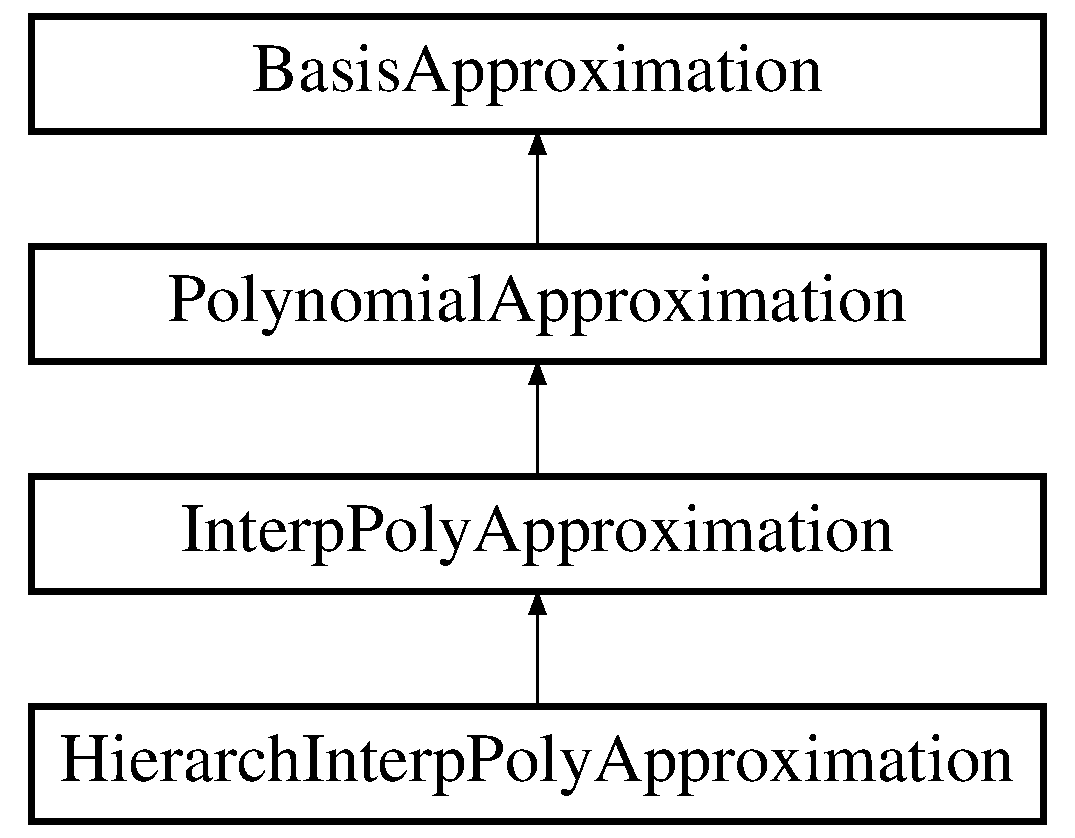
\includegraphics[height=4.000000cm]{classPecos_1_1HierarchInterpPolyApproximation}
\end{center}
\end{figure}
\subsection*{Public Member Functions}
\begin{DoxyCompactItemize}
\item 
\hyperlink{classPecos_1_1HierarchInterpPolyApproximation_a7a8667f6bece197e5c58ffa0a65bbbf0}{Hierarch\+Interp\+Poly\+Approximation} (const \hyperlink{classPecos_1_1SharedBasisApproxData}{Shared\+Basis\+Approx\+Data} \&shared\+\_\+data)\label{classPecos_1_1HierarchInterpPolyApproximation_a7a8667f6bece197e5c58ffa0a65bbbf0}

\begin{DoxyCompactList}\small\item\em Default constructor. \end{DoxyCompactList}\item 
\hyperlink{classPecos_1_1HierarchInterpPolyApproximation_a8a74e4730090c782a9d0973a02f003ea}{$\sim$\+Hierarch\+Interp\+Poly\+Approximation} ()\label{classPecos_1_1HierarchInterpPolyApproximation_a8a74e4730090c782a9d0973a02f003ea}

\begin{DoxyCompactList}\small\item\em destructor \end{DoxyCompactList}\end{DoxyCompactItemize}
\subsection*{Protected Member Functions}
\begin{DoxyCompactItemize}
\item 
void \hyperlink{classPecos_1_1HierarchInterpPolyApproximation_a37ef37829b412fefa40d53b395846781}{allocate\+\_\+arrays} ()\label{classPecos_1_1HierarchInterpPolyApproximation_a37ef37829b412fefa40d53b395846781}

\begin{DoxyCompactList}\small\item\em size expansion\+Type\{1,2\}Coeffs and expansion\+Type1\+Coeff\+Grads \end{DoxyCompactList}\item 
void \hyperlink{classPecos_1_1HierarchInterpPolyApproximation_aef8f0c32bdeff7756a9c614607c03058}{compute\+\_\+coefficients} (size\+\_\+t index=\+\_\+\+N\+P\+OS)\label{classPecos_1_1HierarchInterpPolyApproximation_aef8f0c32bdeff7756a9c614607c03058}

\begin{DoxyCompactList}\small\item\em calculate the approximation coefficients using a set of surrogate data \end{DoxyCompactList}\item 
void \hyperlink{classPecos_1_1HierarchInterpPolyApproximation_a8ba12605934048176c1d1c5722465523}{increment\+\_\+coefficients} (size\+\_\+t index=\+\_\+\+N\+P\+OS)\label{classPecos_1_1HierarchInterpPolyApproximation_a8ba12605934048176c1d1c5722465523}

\begin{DoxyCompactList}\small\item\em update the coefficients for the expansion of interpolation polynomials\+: increment expansion\{Type1\+Coeffs,Type2\+Coeffs,Type1\+Coeff\+Grads\} \end{DoxyCompactList}\item 
void \hyperlink{classPecos_1_1HierarchInterpPolyApproximation_a662fd880fee0ed53f1e3383c41d6b792}{decrement\+\_\+coefficients} (bool save\+\_\+data)\label{classPecos_1_1HierarchInterpPolyApproximation_a662fd880fee0ed53f1e3383c41d6b792}

\begin{DoxyCompactList}\small\item\em restore the coefficients to their previous state prior to last increment\+: decrement expansion\{Type1\+Coeffs,Type2\+Coeffs,Type1\+Coeff\+Grads\} \end{DoxyCompactList}\item 
void \hyperlink{classPecos_1_1HierarchInterpPolyApproximation_a150c32326f6c12d2303806005715706e}{push\+\_\+coefficients} ()\label{classPecos_1_1HierarchInterpPolyApproximation_a150c32326f6c12d2303806005715706e}

\begin{DoxyCompactList}\small\item\em restore the coefficients to a previously incremented state as identified by the current increment to the Smolyak multi index\+: push expansion\{Type1\+Coeffs,Type2\+Coeffs,Type1\+Coeff\+Grads\} \end{DoxyCompactList}\item 
void \hyperlink{classPecos_1_1HierarchInterpPolyApproximation_a742e0217d6f681e08f401409771f4f4a}{finalize\+\_\+coefficients} ()\label{classPecos_1_1HierarchInterpPolyApproximation_a742e0217d6f681e08f401409771f4f4a}

\begin{DoxyCompactList}\small\item\em finalize the coefficients by applying all previously evaluated increments\+: finalize expansion\{Type1\+Coeffs,Type2\+Coeffs,Type1\+Coeff\+Grads\} \end{DoxyCompactList}\item 
void \hyperlink{classPecos_1_1HierarchInterpPolyApproximation_abc17a7104c33d8146f4a0ee7b6c6f37a}{store\+\_\+coefficients} (size\+\_\+t index=\+\_\+\+N\+P\+OS)\label{classPecos_1_1HierarchInterpPolyApproximation_abc17a7104c33d8146f4a0ee7b6c6f37a}

\begin{DoxyCompactList}\small\item\em store current state within stored\+Exp\+Type\{1\+Coeffs,2\+Coeffs,1\+Coeff\+Grads\} \end{DoxyCompactList}\item 
void \hyperlink{classPecos_1_1HierarchInterpPolyApproximation_ad05b093ee96314c9e05bad8e06c2dae7}{restore\+\_\+coefficients} (size\+\_\+t index=\+\_\+\+N\+P\+OS)\label{classPecos_1_1HierarchInterpPolyApproximation_ad05b093ee96314c9e05bad8e06c2dae7}

\begin{DoxyCompactList}\small\item\em restore previous state from stored\+Exp\+Type\{1\+Coeffs,2\+Coeffs,1\+Coeff\+Grads\} \end{DoxyCompactList}\item 
void \hyperlink{classPecos_1_1HierarchInterpPolyApproximation_af5c6af74d2c8c5575fefb46ce55af90d}{swap\+\_\+coefficients} (size\+\_\+t index)\label{classPecos_1_1HierarchInterpPolyApproximation_af5c6af74d2c8c5575fefb46ce55af90d}

\begin{DoxyCompactList}\small\item\em swap stored\+Exp\+Type\{1\+Coeffs,2\+Coeffs,1\+Coeff\+Grads\}\mbox{[}index\mbox{]} with active current data \end{DoxyCompactList}\item 
void \hyperlink{classPecos_1_1HierarchInterpPolyApproximation_a63d12cc6021fda4896b8738d72dfcc86}{remove\+\_\+stored\+\_\+coefficients} (size\+\_\+t index=\+\_\+\+N\+P\+OS)\label{classPecos_1_1HierarchInterpPolyApproximation_a63d12cc6021fda4896b8738d72dfcc86}

\begin{DoxyCompactList}\small\item\em remove a redundant entry from stored\+Exp\+Type\{1\+Coeffs,2\+Coeffs,1\+Coeff\+Grads\} prior to combine\+\_\+coefficients (default is pop\+\_\+back) \end{DoxyCompactList}\item 
void \hyperlink{classPecos_1_1HierarchInterpPolyApproximation_ae4337960917eda26a5672e5c6afbb62a}{clear\+\_\+stored} ()\label{classPecos_1_1HierarchInterpPolyApproximation_ae4337960917eda26a5672e5c6afbb62a}

\begin{DoxyCompactList}\small\item\em clear stored\+Exp\+Type\{1\+Coeffs,2\+Coeffs,1\+Coeff\+Grads\} \end{DoxyCompactList}\item 
void \hyperlink{classPecos_1_1HierarchInterpPolyApproximation_a7c794213befc83c9f90137f22e4cd39d}{combine\+\_\+coefficients} (size\+\_\+t swap\+\_\+index)\label{classPecos_1_1HierarchInterpPolyApproximation_a7c794213befc83c9f90137f22e4cd39d}

\begin{DoxyCompactList}\small\item\em augment current interpolant using stored\+Exp\+Type\{1\+Coeffs,2\+Coeffs,1\+Coeff\+Grads\} \end{DoxyCompactList}\item 
void \hyperlink{classPecos_1_1HierarchInterpPolyApproximation_a9e2f6de3dafca8df624fef2a132b5185}{integrate\+\_\+response\+\_\+moments} (size\+\_\+t num\+\_\+moments)\label{classPecos_1_1HierarchInterpPolyApproximation_a9e2f6de3dafca8df624fef2a132b5185}

\begin{DoxyCompactList}\small\item\em compute moments of response using numerical integration \end{DoxyCompactList}\item 
void \hyperlink{classPecos_1_1HierarchInterpPolyApproximation_a611ac6de1665bc1197922b77823250c2}{integrate\+\_\+expansion\+\_\+moments} (size\+\_\+t num\+\_\+moments)\label{classPecos_1_1HierarchInterpPolyApproximation_a611ac6de1665bc1197922b77823250c2}

\begin{DoxyCompactList}\small\item\em compute moments of expansion using numerical integration \end{DoxyCompactList}\item 
Real \hyperlink{classPecos_1_1HierarchInterpPolyApproximation_a7bc9dcdf32fc46f97e286268c1ac51b0}{value} (const Real\+Vector \&x)\label{classPecos_1_1HierarchInterpPolyApproximation_a7bc9dcdf32fc46f97e286268c1ac51b0}

\begin{DoxyCompactList}\small\item\em retrieve the approximate function value for a given parameter vector \end{DoxyCompactList}\item 
const Real\+Vector \& \hyperlink{classPecos_1_1HierarchInterpPolyApproximation_ae3b6ea541392b74cf0cc8758e206277c}{gradient\+\_\+basis\+\_\+variables} (const Real\+Vector \&x)\label{classPecos_1_1HierarchInterpPolyApproximation_ae3b6ea541392b74cf0cc8758e206277c}

\begin{DoxyCompactList}\small\item\em retrieve the gradient for a response expansion with respect to all variables included in the polynomial bases using the given parameter vector and default D\+VV \end{DoxyCompactList}\item 
const Real\+Vector \& \hyperlink{classPecos_1_1HierarchInterpPolyApproximation_a3ffb563ae1658344bfc2ad882def9e7c}{gradient\+\_\+basis\+\_\+variables} (const Real\+Vector \&x, const Sizet\+Array \&dvv)\label{classPecos_1_1HierarchInterpPolyApproximation_a3ffb563ae1658344bfc2ad882def9e7c}

\begin{DoxyCompactList}\small\item\em retrieve the gradient for a response expansion with respect to variables included in the polynomial basis for a given parameter vector and a given D\+VV subset \end{DoxyCompactList}\item 
const Real\+Vector \& \hyperlink{classPecos_1_1HierarchInterpPolyApproximation_a518e8604f973a4b161a9b5718a0aa25e}{gradient\+\_\+nonbasis\+\_\+variables} (const Real\+Vector \&x)\label{classPecos_1_1HierarchInterpPolyApproximation_a518e8604f973a4b161a9b5718a0aa25e}

\begin{DoxyCompactList}\small\item\em retrieve the gradient for a response expansion with respect to all variables not included in the polynomial bases (nonprobabilistic variables such as design or epistemic when not in \char`\"{}all\char`\"{} mode) using the given parameter vector and default D\+VV \end{DoxyCompactList}\item 
const Real\+Sym\+Matrix \& \hyperlink{classPecos_1_1HierarchInterpPolyApproximation_a830729654265d84af637960f8c63f2bc}{hessian\+\_\+basis\+\_\+variables} (const Real\+Vector \&x)\label{classPecos_1_1HierarchInterpPolyApproximation_a830729654265d84af637960f8c63f2bc}

\begin{DoxyCompactList}\small\item\em retrieve the Hessian of the response expansion with respect to all variables included in the polynomial basis (e.\+g., probabilistic variables) for a given parameter vector \end{DoxyCompactList}\item 
Real \hyperlink{classPecos_1_1HierarchInterpPolyApproximation_a1abe918dbdc66ac0fde85f1ab3c061af}{stored\+\_\+value} (const Real\+Vector \&x, size\+\_\+t index)\label{classPecos_1_1HierarchInterpPolyApproximation_a1abe918dbdc66ac0fde85f1ab3c061af}

\begin{DoxyCompactList}\small\item\em retrieve the response value for a stored expansion using the given parameter vector \end{DoxyCompactList}\item 
const Real\+Vector \& \hyperlink{classPecos_1_1HierarchInterpPolyApproximation_a7689fc058e2efdde6ce4dfe898864592}{stored\+\_\+gradient\+\_\+basis\+\_\+variables} (const Real\+Vector \&x, size\+\_\+t index)\label{classPecos_1_1HierarchInterpPolyApproximation_a7689fc058e2efdde6ce4dfe898864592}

\begin{DoxyCompactList}\small\item\em retrieve the response gradient for a stored expansion with respect to all variables included in the polynomial bases; evaluate for the given parameter vector. \end{DoxyCompactList}\item 
const Real\+Vector \& \hyperlink{classPecos_1_1HierarchInterpPolyApproximation_af0c9184d9a0da7b0e3d0d3ecbfc8f434}{stored\+\_\+gradient\+\_\+nonbasis\+\_\+variables} (const Real\+Vector \&x, size\+\_\+t index)\label{classPecos_1_1HierarchInterpPolyApproximation_af0c9184d9a0da7b0e3d0d3ecbfc8f434}

\begin{DoxyCompactList}\small\item\em retrieve the response gradient for a stored expansion with respect to all variables not included in the polynomial bases; evaluate for the given parameter vector. \end{DoxyCompactList}\item 
Real \hyperlink{classPecos_1_1HierarchInterpPolyApproximation_adc6f262952d05a33ff68cae37929cbb2}{mean} ()\label{classPecos_1_1HierarchInterpPolyApproximation_adc6f262952d05a33ff68cae37929cbb2}

\begin{DoxyCompactList}\small\item\em return the mean of the expansion, treating all variables as random \end{DoxyCompactList}\item 
Real \hyperlink{classPecos_1_1HierarchInterpPolyApproximation_aed107df248a4555c052446fbc10a8e61}{mean} (const Real\+Vector \&x)\label{classPecos_1_1HierarchInterpPolyApproximation_aed107df248a4555c052446fbc10a8e61}

\begin{DoxyCompactList}\small\item\em return the mean of the expansion for a given parameter vector, treating a subset of the variables as random \end{DoxyCompactList}\item 
const Real\+Vector \& \hyperlink{classPecos_1_1HierarchInterpPolyApproximation_a069c87a26fdb4b09af68db26abd646a0}{mean\+\_\+gradient} ()
\item 
const Real\+Vector \& \hyperlink{classPecos_1_1HierarchInterpPolyApproximation_a24f2edc21c9887121cda78faae1c1475}{mean\+\_\+gradient} (const Real\+Vector \&x, const Sizet\+Array \&dvv)
\item 
Real \hyperlink{classPecos_1_1HierarchInterpPolyApproximation_a38f6da77468be17e02ce38af2c0976c3}{variance} ()\label{classPecos_1_1HierarchInterpPolyApproximation_a38f6da77468be17e02ce38af2c0976c3}

\begin{DoxyCompactList}\small\item\em return the variance of the expansion, treating all variables as random \end{DoxyCompactList}\item 
Real \hyperlink{classPecos_1_1HierarchInterpPolyApproximation_acbdcb523a161d7d3a5cc190796e84ede}{variance} (const Real\+Vector \&x)\label{classPecos_1_1HierarchInterpPolyApproximation_acbdcb523a161d7d3a5cc190796e84ede}

\begin{DoxyCompactList}\small\item\em return the variance of the expansion for a given parameter vector, treating a subset of the variables as random \end{DoxyCompactList}\item 
const Real\+Vector \& \hyperlink{classPecos_1_1HierarchInterpPolyApproximation_ae898fc2f42f1077268f89fc2e9f2c71c}{variance\+\_\+gradient} ()
\item 
const Real\+Vector \& \hyperlink{classPecos_1_1HierarchInterpPolyApproximation_a791e127a445f8a6c9c3a7966d12c1431}{variance\+\_\+gradient} (const Real\+Vector \&x, const Sizet\+Array \&dvv)
\item 
Real \hyperlink{classPecos_1_1HierarchInterpPolyApproximation_ac0085912d4abb9caa3f480b9c6778c0e}{covariance} (\hyperlink{classPecos_1_1PolynomialApproximation}{Polynomial\+Approximation} $\ast$poly\+\_\+approx\+\_\+2)\label{classPecos_1_1HierarchInterpPolyApproximation_ac0085912d4abb9caa3f480b9c6778c0e}

\begin{DoxyCompactList}\small\item\em return the covariance between two response expansions, treating all variables as random \end{DoxyCompactList}\item 
Real \hyperlink{classPecos_1_1HierarchInterpPolyApproximation_afc1731a3d89818d49c03a3c20a7a2898}{covariance} (const Real\+Vector \&x, \hyperlink{classPecos_1_1PolynomialApproximation}{Polynomial\+Approximation} $\ast$poly\+\_\+approx\+\_\+2)\label{classPecos_1_1HierarchInterpPolyApproximation_afc1731a3d89818d49c03a3c20a7a2898}

\begin{DoxyCompactList}\small\item\em return the covariance between two response expansions for a given parameter vector, treating a subset of the variables as random \end{DoxyCompactList}\item 
Real \hyperlink{classPecos_1_1HierarchInterpPolyApproximation_ae3f6a8d87917102636d171f5c86a2fb5}{delta\+\_\+covariance} (\hyperlink{classPecos_1_1PolynomialApproximation}{Polynomial\+Approximation} $\ast$poly\+\_\+approx\+\_\+2)\label{classPecos_1_1HierarchInterpPolyApproximation_ae3f6a8d87917102636d171f5c86a2fb5}

\begin{DoxyCompactList}\small\item\em return the change in covariance between two response expansions, treating all variables as random \end{DoxyCompactList}\item 
Real \hyperlink{classPecos_1_1HierarchInterpPolyApproximation_a5a89afe07fb520282fa35dfc9ca2b0a1}{delta\+\_\+covariance} (const Real\+Vector \&x, \hyperlink{classPecos_1_1PolynomialApproximation}{Polynomial\+Approximation} $\ast$poly\+\_\+approx\+\_\+2)\label{classPecos_1_1HierarchInterpPolyApproximation_a5a89afe07fb520282fa35dfc9ca2b0a1}

\begin{DoxyCompactList}\small\item\em return the change in covariance between two response expansions for a given parameter vector, treating a subset of the variables as random \end{DoxyCompactList}\item 
Real \hyperlink{classPecos_1_1HierarchInterpPolyApproximation_aa276ec09d706b03780f9bc01af40514e}{delta\+\_\+mean} ()\label{classPecos_1_1HierarchInterpPolyApproximation_aa276ec09d706b03780f9bc01af40514e}

\begin{DoxyCompactList}\small\item\em return the change in mean between two response expansions, treating all variables as random \end{DoxyCompactList}\item 
Real \hyperlink{classPecos_1_1HierarchInterpPolyApproximation_a47a27e963aa71bb3dfc2aa623f7f3e92}{delta\+\_\+mean} (const Real\+Vector \&x)\label{classPecos_1_1HierarchInterpPolyApproximation_a47a27e963aa71bb3dfc2aa623f7f3e92}

\begin{DoxyCompactList}\small\item\em return the change in mean between two response expansions, treating a subset of the variables as random \end{DoxyCompactList}\item 
Real \hyperlink{classPecos_1_1HierarchInterpPolyApproximation_a91067291a8c8ca1f582e24706aac5ea7}{delta\+\_\+std\+\_\+deviation} ()\label{classPecos_1_1HierarchInterpPolyApproximation_a91067291a8c8ca1f582e24706aac5ea7}

\begin{DoxyCompactList}\small\item\em return the change in standard deviation between two response expansions, treating all variables as random \end{DoxyCompactList}\item 
Real \hyperlink{classPecos_1_1HierarchInterpPolyApproximation_a4755135ffbf0475a447f71d7b782afa8}{delta\+\_\+std\+\_\+deviation} (const Real\+Vector \&x)\label{classPecos_1_1HierarchInterpPolyApproximation_a4755135ffbf0475a447f71d7b782afa8}

\begin{DoxyCompactList}\small\item\em return the change in standard deviation between two response expansions, treating a subset of the variables as random \end{DoxyCompactList}\item 
Real \hyperlink{classPecos_1_1HierarchInterpPolyApproximation_af4a1a73ea647b8989096db81a7e36278}{delta\+\_\+beta} (bool cdf\+\_\+flag, Real z\+\_\+bar)\label{classPecos_1_1HierarchInterpPolyApproximation_af4a1a73ea647b8989096db81a7e36278}

\begin{DoxyCompactList}\small\item\em return the change in reliability index (mapped from z\+\_\+bar) between two response expansions, treating all variables as random \end{DoxyCompactList}\item 
Real \hyperlink{classPecos_1_1HierarchInterpPolyApproximation_ad878382953dfa3146f4862f6195ea351}{delta\+\_\+beta} (const Real\+Vector \&x, bool cdf\+\_\+flag, Real z\+\_\+bar)\label{classPecos_1_1HierarchInterpPolyApproximation_ad878382953dfa3146f4862f6195ea351}

\begin{DoxyCompactList}\small\item\em return the change in reliability index (mapped from z\+\_\+bar) between two response expansions, treating a subset of the variables as random \end{DoxyCompactList}\item 
Real \hyperlink{classPecos_1_1HierarchInterpPolyApproximation_a677b7ca69b5b17169b3f6e3ccb972ce6}{delta\+\_\+z} (bool cdf\+\_\+flag, Real beta\+\_\+bar)\label{classPecos_1_1HierarchInterpPolyApproximation_a677b7ca69b5b17169b3f6e3ccb972ce6}

\begin{DoxyCompactList}\small\item\em return the change in response level (mapped from beta\+\_\+bar) between two response expansions, treating all variables as random \end{DoxyCompactList}\item 
Real \hyperlink{classPecos_1_1HierarchInterpPolyApproximation_a3280b1f280ca2af6d965d5562fc42770}{delta\+\_\+z} (const Real\+Vector \&x, bool cdf\+\_\+flag, Real beta\+\_\+bar)\label{classPecos_1_1HierarchInterpPolyApproximation_a3280b1f280ca2af6d965d5562fc42770}

\begin{DoxyCompactList}\small\item\em return the change in response level (mapped from beta\+\_\+bar) between two response expansions, treating a subset of the variables as random \end{DoxyCompactList}\item 
void {\bfseries compute\+\_\+total\+\_\+sobol\+\_\+indices} ()\label{classPecos_1_1HierarchInterpPolyApproximation_a9b445d773d12ed85eb56bb73f6d7e540}

\item 
void \hyperlink{classPecos_1_1HierarchInterpPolyApproximation_a6eb2548a8c786f48478fabb6377be779}{compute\+\_\+partial\+\_\+variance} (const Bit\+Array \&set\+\_\+value)
\end{DoxyCompactItemize}
\subsection*{Private Member Functions}
\begin{DoxyCompactItemize}
\item 
Real \hyperlink{classPecos_1_1HierarchInterpPolyApproximation_a74a9d557c508cd043c0c444dc722ed6d}{value} (const Real\+Vector \&x, const U\+Short3\+D\+Array \&sm\+\_\+mi, const U\+Short4\+D\+Array \&key, const Real\+Vector2\+D\+Array \&t1\+\_\+coeffs, const Real\+Matrix2\+D\+Array \&t2\+\_\+coeffs, unsigned short level)\label{classPecos_1_1HierarchInterpPolyApproximation_a74a9d557c508cd043c0c444dc722ed6d}

\begin{DoxyCompactList}\small\item\em compute the value at a point for a particular interpolation level \end{DoxyCompactList}\item 
Real \hyperlink{classPecos_1_1HierarchInterpPolyApproximation_a814452cf28de0138f1095f9cbe1d5471}{value} (const Real\+Vector \&x, const U\+Short3\+D\+Array \&sm\+\_\+mi, const U\+Short4\+D\+Array \&key, const Real\+Vector2\+D\+Array \&t1\+\_\+coeffs, const Real\+Matrix2\+D\+Array \&t2\+\_\+coeffs, unsigned short level, const Sizet\+List \&subset\+\_\+indices)
\begin{DoxyCompactList}\small\item\em compute the value at a point for a particular interpolation level and for a specified subset of the variables \end{DoxyCompactList}\item 
const Real\+Vector \& \hyperlink{classPecos_1_1HierarchInterpPolyApproximation_a143aad43c78dbe10aec18749a4de4dc0}{gradient\+\_\+basis\+\_\+variables} (const Real\+Vector \&x, const U\+Short3\+D\+Array \&sm\+\_\+mi, const U\+Short4\+D\+Array \&key, const Real\+Vector2\+D\+Array \&t1\+\_\+coeffs, const Real\+Matrix2\+D\+Array \&t2\+\_\+coeffs, unsigned short level)\label{classPecos_1_1HierarchInterpPolyApproximation_a143aad43c78dbe10aec18749a4de4dc0}

\begin{DoxyCompactList}\small\item\em compute the approximate gradient with respect to the basis variables at a particular point for a particular interpolation level \end{DoxyCompactList}\item 
const Real\+Vector \& \hyperlink{classPecos_1_1HierarchInterpPolyApproximation_afaffbe62512edfaee23db02601ef43c6}{gradient\+\_\+basis\+\_\+variables} (const Real\+Vector \&x, const U\+Short3\+D\+Array \&sm\+\_\+mi, const U\+Short4\+D\+Array \&key, const Real\+Vector2\+D\+Array \&t1\+\_\+coeffs, const Real\+Matrix2\+D\+Array \&t2\+\_\+coeffs, unsigned short level, const Sizet\+List \&subset\+\_\+indices)\label{classPecos_1_1HierarchInterpPolyApproximation_afaffbe62512edfaee23db02601ef43c6}

\begin{DoxyCompactList}\small\item\em compute the approximate gradient with respect to the basis variables at a particular point for a particular interpolation level \end{DoxyCompactList}\item 
const Real\+Vector \& \hyperlink{classPecos_1_1HierarchInterpPolyApproximation_a9139778c2ccb10bbab1e39350d83723f}{gradient\+\_\+basis\+\_\+variables} (const Real\+Vector \&x, const U\+Short3\+D\+Array \&sm\+\_\+mi, const U\+Short4\+D\+Array \&key, const Real\+Vector2\+D\+Array \&t1\+\_\+coeffs, const Real\+Matrix2\+D\+Array \&t2\+\_\+coeffs, const Sizet\+Array \&dvv, unsigned short level)\label{classPecos_1_1HierarchInterpPolyApproximation_a9139778c2ccb10bbab1e39350d83723f}

\begin{DoxyCompactList}\small\item\em compute the approximate gradient with respect to the basis variables for a particular point, interpolation level, and D\+VV \end{DoxyCompactList}\item 
const Real\+Vector \& \hyperlink{classPecos_1_1HierarchInterpPolyApproximation_a1de3411a13a420dc114cd02c96ebc4d2}{gradient\+\_\+nonbasis\+\_\+variables} (const Real\+Vector \&x, const U\+Short3\+D\+Array \&sm\+\_\+mi, const U\+Short4\+D\+Array \&key, const Real\+Matrix2\+D\+Array \&t1\+\_\+coeff\+\_\+grads, unsigned short level)\label{classPecos_1_1HierarchInterpPolyApproximation_a1de3411a13a420dc114cd02c96ebc4d2}

\begin{DoxyCompactList}\small\item\em compute the approximate gradient with respect to the nonbasis variables at a particular point for a particular interpolation level \end{DoxyCompactList}\item 
void \hyperlink{classPecos_1_1HierarchInterpPolyApproximation_a109b517f8ff17e6706d3d4fdb9e76961}{increment\+\_\+current\+\_\+from\+\_\+reference} ()\label{classPecos_1_1HierarchInterpPolyApproximation_a109b517f8ff17e6706d3d4fdb9e76961}

\begin{DoxyCompactList}\small\item\em update bookkeeping when adding a grid increment relative to the grid reference \end{DoxyCompactList}\item 
void \hyperlink{classPecos_1_1HierarchInterpPolyApproximation_a06231ad34b1b67dbcb03127186bf3a06}{decrement\+\_\+current\+\_\+to\+\_\+reference} ()\label{classPecos_1_1HierarchInterpPolyApproximation_a06231ad34b1b67dbcb03127186bf3a06}

\begin{DoxyCompactList}\small\item\em update bookkeeping when removing a grid increment and returning to the grid reference \end{DoxyCompactList}\item 
Real \hyperlink{classPecos_1_1HierarchInterpPolyApproximation_af5705082b10f5d61987169b5a84f27dd}{reference\+\_\+mean} (const U\+Short2\+D\+Array \&ref\+\_\+key)\label{classPecos_1_1HierarchInterpPolyApproximation_af5705082b10f5d61987169b5a84f27dd}

\begin{DoxyCompactList}\small\item\em compute the reference mean, excluding the current grid increment, using ref\+\_\+key \end{DoxyCompactList}\item 
Real \hyperlink{classPecos_1_1HierarchInterpPolyApproximation_a9cb0a71afa77132fae9eac948c782880}{reference\+\_\+mean} (const Real\+Vector \&x, const U\+Short2\+D\+Array \&ref\+\_\+key)\label{classPecos_1_1HierarchInterpPolyApproximation_a9cb0a71afa77132fae9eac948c782880}

\begin{DoxyCompactList}\small\item\em compute the reference mean, excluding the current grid increment, using ref\+\_\+key \end{DoxyCompactList}\item 
Real \hyperlink{classPecos_1_1HierarchInterpPolyApproximation_a6a25f632a3b1b91ac183dd55320eaad7}{reference\+\_\+variance} (const U\+Short2\+D\+Array \&ref\+\_\+key)\label{classPecos_1_1HierarchInterpPolyApproximation_a6a25f632a3b1b91ac183dd55320eaad7}

\begin{DoxyCompactList}\small\item\em compute the reference variance, excluding the current grid increment, using ref\+\_\+key \end{DoxyCompactList}\item 
Real \hyperlink{classPecos_1_1HierarchInterpPolyApproximation_a5a884802084505eb75bda915e649e9eb}{reference\+\_\+variance} (const Real\+Vector \&x, const U\+Short2\+D\+Array \&ref\+\_\+key)\label{classPecos_1_1HierarchInterpPolyApproximation_a5a884802084505eb75bda915e649e9eb}

\begin{DoxyCompactList}\small\item\em compute the reference variance, excluding the current grid increment, using ref\+\_\+key \end{DoxyCompactList}\item 
Real \hyperlink{classPecos_1_1HierarchInterpPolyApproximation_a6a1e7ea9782d28b034be7aedf7197c7d}{delta\+\_\+covariance} (\hyperlink{classPecos_1_1PolynomialApproximation}{Polynomial\+Approximation} $\ast$poly\+\_\+approx\+\_\+2, const U\+Short2\+D\+Array \&ref\+\_\+key, const U\+Short2\+D\+Array \&incr\+\_\+key)\label{classPecos_1_1HierarchInterpPolyApproximation_a6a1e7ea9782d28b034be7aedf7197c7d}

\begin{DoxyCompactList}\small\item\em compute the covariance increment due to the current grid increment \end{DoxyCompactList}\item 
Real \hyperlink{classPecos_1_1HierarchInterpPolyApproximation_a931312a9e825efa5139f8110c2e48e7b}{delta\+\_\+covariance} (const Real\+Vector \&x, \hyperlink{classPecos_1_1PolynomialApproximation}{Polynomial\+Approximation} $\ast$poly\+\_\+approx\+\_\+2, const U\+Short2\+D\+Array \&ref\+\_\+key, const U\+Short2\+D\+Array \&incr\+\_\+key)\label{classPecos_1_1HierarchInterpPolyApproximation_a931312a9e825efa5139f8110c2e48e7b}

\begin{DoxyCompactList}\small\item\em compute the covariance increment due to the current grid increment \end{DoxyCompactList}\item 
Real \hyperlink{classPecos_1_1HierarchInterpPolyApproximation_a2ad19ef780b2f6df0a0fa7c6e5354b87}{delta\+\_\+mean} (const U\+Short2\+D\+Array \&incr\+\_\+key)\label{classPecos_1_1HierarchInterpPolyApproximation_a2ad19ef780b2f6df0a0fa7c6e5354b87}

\begin{DoxyCompactList}\small\item\em compute the mean increment due to the current grid increment \end{DoxyCompactList}\item 
Real \hyperlink{classPecos_1_1HierarchInterpPolyApproximation_a4aa71b3572421587c1982eaf73829532}{delta\+\_\+mean} (const Real\+Vector \&x, const U\+Short2\+D\+Array \&incr\+\_\+key)\label{classPecos_1_1HierarchInterpPolyApproximation_a4aa71b3572421587c1982eaf73829532}

\begin{DoxyCompactList}\small\item\em compute the mean increment due to the current grid increment \end{DoxyCompactList}\item 
Real \hyperlink{classPecos_1_1HierarchInterpPolyApproximation_a9c557ad7598b71069d615266242487a5}{delta\+\_\+variance} (const U\+Short2\+D\+Array \&ref\+\_\+key, const U\+Short2\+D\+Array \&incr\+\_\+key)\label{classPecos_1_1HierarchInterpPolyApproximation_a9c557ad7598b71069d615266242487a5}

\begin{DoxyCompactList}\small\item\em compute the variance increment due to the current grid increment \end{DoxyCompactList}\item 
Real \hyperlink{classPecos_1_1HierarchInterpPolyApproximation_a80b3297ec61c03c246326cbcbc2fd4b0}{delta\+\_\+variance} (const Real\+Vector \&x, const U\+Short2\+D\+Array \&ref\+\_\+key, const U\+Short2\+D\+Array \&incr\+\_\+key)\label{classPecos_1_1HierarchInterpPolyApproximation_a80b3297ec61c03c246326cbcbc2fd4b0}

\begin{DoxyCompactList}\small\item\em compute the variance increment due to the current grid increment \end{DoxyCompactList}\item 
Real \hyperlink{classPecos_1_1HierarchInterpPolyApproximation_aaf63c8320565d50ab4acf612438e93be}{delta\+\_\+std\+\_\+deviation} (const U\+Short2\+D\+Array \&ref\+\_\+key, const U\+Short2\+D\+Array \&incr\+\_\+key)\label{classPecos_1_1HierarchInterpPolyApproximation_aaf63c8320565d50ab4acf612438e93be}

\begin{DoxyCompactList}\small\item\em compute the standard deviation increment due to the current grid increment \end{DoxyCompactList}\item 
Real \hyperlink{classPecos_1_1HierarchInterpPolyApproximation_a3d0406d60c6804cb817a95cc61a5dd93}{delta\+\_\+std\+\_\+deviation} (const Real\+Vector \&x, const U\+Short2\+D\+Array \&ref\+\_\+key, const U\+Short2\+D\+Array \&incr\+\_\+key)\label{classPecos_1_1HierarchInterpPolyApproximation_a3d0406d60c6804cb817a95cc61a5dd93}

\begin{DoxyCompactList}\small\item\em compute the standard deviation increment due to the current grid increment \end{DoxyCompactList}\item 
Real \hyperlink{classPecos_1_1HierarchInterpPolyApproximation_a0f868257947afc0ce1b58d194bc414e8}{delta\+\_\+beta} (bool cdf\+\_\+flag, Real z\+\_\+bar, const U\+Short2\+D\+Array \&ref\+\_\+key, const U\+Short2\+D\+Array \&incr\+\_\+key)\label{classPecos_1_1HierarchInterpPolyApproximation_a0f868257947afc0ce1b58d194bc414e8}

\begin{DoxyCompactList}\small\item\em compute the reliability index increment due to the current grid increment \end{DoxyCompactList}\item 
Real \hyperlink{classPecos_1_1HierarchInterpPolyApproximation_a23bf48e6ed8ab2c0c04229866effa967}{delta\+\_\+beta} (const Real\+Vector \&x, bool cdf\+\_\+flag, Real z\+\_\+bar, const U\+Short2\+D\+Array \&ref\+\_\+key, const U\+Short2\+D\+Array \&incr\+\_\+key)\label{classPecos_1_1HierarchInterpPolyApproximation_a23bf48e6ed8ab2c0c04229866effa967}

\begin{DoxyCompactList}\small\item\em compute the reliability index increment due to the current grid increment \end{DoxyCompactList}\item 
Real \hyperlink{classPecos_1_1HierarchInterpPolyApproximation_aa98a30aa3967a620f7adeda20f3ebbeb}{delta\+\_\+beta\+\_\+map} (Real mu0, Real delta\+\_\+mu, Real var0, Real delta\+\_\+sigma, bool cdf\+\_\+flag, Real z\+\_\+bar)\label{classPecos_1_1HierarchInterpPolyApproximation_aa98a30aa3967a620f7adeda20f3ebbeb}

\begin{DoxyCompactList}\small\item\em shared logic for handling exceptional cases \end{DoxyCompactList}\item 
Real \hyperlink{classPecos_1_1HierarchInterpPolyApproximation_a0cbb05caf7c944d49bff491d393a4236}{delta\+\_\+z} (bool cdf\+\_\+flag, Real beta\+\_\+bar, const U\+Short2\+D\+Array \&ref\+\_\+key, const U\+Short2\+D\+Array \&incr\+\_\+key)\label{classPecos_1_1HierarchInterpPolyApproximation_a0cbb05caf7c944d49bff491d393a4236}

\begin{DoxyCompactList}\small\item\em compute the response level increment due to the current grid increment \end{DoxyCompactList}\item 
Real \hyperlink{classPecos_1_1HierarchInterpPolyApproximation_a0a9f4f936740e46b517449a7e935bb2b}{delta\+\_\+z} (const Real\+Vector \&x, bool cdf\+\_\+flag, Real beta\+\_\+bar, const U\+Short2\+D\+Array \&ref\+\_\+key, const U\+Short2\+D\+Array \&incr\+\_\+key)\label{classPecos_1_1HierarchInterpPolyApproximation_a0a9f4f936740e46b517449a7e935bb2b}

\begin{DoxyCompactList}\small\item\em compute the response level increment due to the current grid increment \end{DoxyCompactList}\item 
void \hyperlink{classPecos_1_1HierarchInterpPolyApproximation_a56d259d2bc9e4b3c7177953e103ed70d}{product\+\_\+interpolant} (\hyperlink{classPecos_1_1HierarchInterpPolyApproximation}{Hierarch\+Interp\+Poly\+Approximation} $\ast$hip\+\_\+approx\+\_\+2, Real\+Vector2\+D\+Array \&r1r2\+\_\+t1\+\_\+coeffs, Real\+Matrix2\+D\+Array \&r1r2\+\_\+t2\+\_\+coeffs, const U\+Short2\+D\+Array \&reference\+\_\+key=U\+Short2\+D\+Array())
\begin{DoxyCompactList}\small\item\em form type 1/2 coefficients for interpolation of R\+\_\+1 R\+\_\+2 \end{DoxyCompactList}\item 
void \hyperlink{classPecos_1_1HierarchInterpPolyApproximation_ad568c5307549ce96de86b1cd5fa0097d}{central\+\_\+product\+\_\+interpolant} (\hyperlink{classPecos_1_1HierarchInterpPolyApproximation}{Hierarch\+Interp\+Poly\+Approximation} $\ast$hip\+\_\+approx\+\_\+2, Real mean\+\_\+1, Real mean\+\_\+2, Real\+Vector2\+D\+Array \&cov\+\_\+t1\+\_\+coeffs, Real\+Matrix2\+D\+Array \&cov\+\_\+t2\+\_\+coeffs, const U\+Short2\+D\+Array \&reference\+\_\+key=U\+Short2\+D\+Array())
\begin{DoxyCompactList}\small\item\em form type 1/2 coefficients for interpolation of (R\+\_\+1 -\/ mu\+\_\+1)(R\+\_\+2 -\/ mu\+\_\+2) \end{DoxyCompactList}\item 
void \hyperlink{classPecos_1_1HierarchInterpPolyApproximation_a0877cb2c939711ebe697928c6649affc}{central\+\_\+product\+\_\+gradient\+\_\+interpolant} (\hyperlink{classPecos_1_1HierarchInterpPolyApproximation}{Hierarch\+Interp\+Poly\+Approximation} $\ast$hip\+\_\+approx\+\_\+2, Real mean\+\_\+1, Real mean\+\_\+2, const Real\+Vector \&mean1\+\_\+grad, const Real\+Vector \&mean2\+\_\+grad, Real\+Matrix2\+D\+Array \&cov\+\_\+t1\+\_\+coeff\+\_\+grads, const U\+Short2\+D\+Array \&reference\+\_\+key=U\+Short2\+D\+Array())\label{classPecos_1_1HierarchInterpPolyApproximation_a0877cb2c939711ebe697928c6649affc}

\begin{DoxyCompactList}\small\item\em form type1 coefficient gradients for interpolation of d/ds \mbox{[}(R\+\_\+1 -\/ mu\+\_\+1)(R\+\_\+2 -\/ mu\+\_\+2)\mbox{]} \end{DoxyCompactList}\item 
Real \hyperlink{classPecos_1_1HierarchInterpPolyApproximation_af379a9ca4f3a57b0288206ca8bf4d726}{expectation} (const Real\+Vector2\+D\+Array \&t1\+\_\+coeffs, const Real\+Matrix2\+D\+Array \&t2\+\_\+coeffs, const U\+Short2\+D\+Array \&set\+\_\+partition=U\+Short2\+D\+Array())\label{classPecos_1_1HierarchInterpPolyApproximation_af379a9ca4f3a57b0288206ca8bf4d726}

\begin{DoxyCompactList}\small\item\em compute the expected value of the interpolant given by t\{1,2\}\+\_\+coeffs using weights from the \hyperlink{classPecos_1_1HierarchSparseGridDriver}{Hierarch\+Sparse\+Grid\+Driver} \end{DoxyCompactList}\item 
Real \hyperlink{classPecos_1_1HierarchInterpPolyApproximation_ac11a36763964807e2496970dd2a7170d}{expectation} (const Real\+Vector2\+D\+Array \&t1\+\_\+coeffs, const Real\+Vector2\+D\+Array \&t1\+\_\+wts, const Real\+Matrix2\+D\+Array \&t2\+\_\+coeffs, const Real\+Matrix2\+D\+Array \&t2\+\_\+wts, const U\+Short2\+D\+Array \&set\+\_\+partition=U\+Short2\+D\+Array())\label{classPecos_1_1HierarchInterpPolyApproximation_ac11a36763964807e2496970dd2a7170d}

\begin{DoxyCompactList}\small\item\em compute the expected value of the interpolant given by t\{1,2\}\+\_\+coeffs using t\{1,2\}\+\_\+wts \end{DoxyCompactList}\item 
Real \hyperlink{classPecos_1_1HierarchInterpPolyApproximation_a025b070b17e6ea1a80bf14b1ab59eeb8}{expectation} (const Real\+Vector \&x, const Real\+Vector2\+D\+Array \&t1\+\_\+coeffs, const Real\+Matrix2\+D\+Array \&t2\+\_\+coeffs, const U\+Short2\+D\+Array \&set\+\_\+partition=U\+Short2\+D\+Array())\label{classPecos_1_1HierarchInterpPolyApproximation_a025b070b17e6ea1a80bf14b1ab59eeb8}

\begin{DoxyCompactList}\small\item\em compute the expected value of the interpolant given by t\{1,2\}\+\_\+coeffs using weights from the \hyperlink{classPecos_1_1HierarchSparseGridDriver}{Hierarch\+Sparse\+Grid\+Driver} \end{DoxyCompactList}\item 
const Real\+Vector \& \hyperlink{classPecos_1_1HierarchInterpPolyApproximation_a923b0e83c2a901b95842cc0f8cdfd038}{expectation\+\_\+gradient} (const Real\+Matrix2\+D\+Array \&t1\+\_\+coeff\+\_\+grads)\label{classPecos_1_1HierarchInterpPolyApproximation_a923b0e83c2a901b95842cc0f8cdfd038}

\begin{DoxyCompactList}\small\item\em compute the expected value of the gradient interpolant given by t1\+\_\+coeff\+\_\+grads using weights from the \hyperlink{classPecos_1_1HierarchSparseGridDriver}{Hierarch\+Sparse\+Grid\+Driver} \end{DoxyCompactList}\item 
const Real\+Vector \& \hyperlink{classPecos_1_1HierarchInterpPolyApproximation_af7cb170e68ec826d583313ef224f47a0}{expectation\+\_\+gradient} (const Real\+Matrix2\+D\+Array \&t1\+\_\+coeff\+\_\+grads, const Real\+Vector2\+D\+Array \&t1\+\_\+wts)
\begin{DoxyCompactList}\small\item\em compute the expected value of the gradient interpolant given by t1\+\_\+coeff\+\_\+grads using t1\+\_\+wts \end{DoxyCompactList}\item 
Real \hyperlink{classPecos_1_1HierarchInterpPolyApproximation_a6e2bc30784df7fe2c7c058f55376a0a4}{expectation\+\_\+gradient} (const Real\+Vector \&x, const Real\+Matrix2\+D\+Array \&t1\+\_\+coeff\+\_\+grads, size\+\_\+t t1cg\+\_\+index)
\begin{DoxyCompactList}\small\item\em compute the expectation of t1\+\_\+coeff\+\_\+grads for index t1cg\+\_\+index \end{DoxyCompactList}\item 
Real \hyperlink{classPecos_1_1HierarchInterpPolyApproximation_ab1ddf31383c7e516aeb07b80339ec461}{expectation\+\_\+gradient} (const Real\+Vector \&x, const Real\+Vector2\+D\+Array \&t1\+\_\+coeffs, const Real\+Matrix2\+D\+Array \&t2\+\_\+coeffs, size\+\_\+t deriv\+\_\+index)
\begin{DoxyCompactList}\small\item\em compute the expectation of the gradient of \{t1,t2\}\+\_\+coeffs for index deriv\+\_\+index \end{DoxyCompactList}\item 
void \hyperlink{classPecos_1_1HierarchInterpPolyApproximation_a9403f7c8e5fbfdb4b2142b088673c533}{increment\+\_\+coefficients} (const U\+Short\+Array \&index\+\_\+set)
\begin{DoxyCompactList}\small\item\em increment expansion\{Type1\+Coeffs,Type2\+Coeffs,Type1\+Coeff\+Grads\} for a single index\+\_\+set \end{DoxyCompactList}\item 
void \hyperlink{classPecos_1_1HierarchInterpPolyApproximation_a85c57e8dbd99dfa66dcd11eda308432e}{push\+\_\+coefficients} (const U\+Short\+Array \&push\+\_\+set)
\begin{DoxyCompactList}\small\item\em move the expansion coefficients for push\+\_\+set from popped\+Exp\{T1\+Coeffs,T2\+Coeffs,T1\+Coeff\+Grads\} to expansion\{Type1\+Coeffs,Type2\+Coeffs,Type1\+Coeff\+Grads\} \end{DoxyCompactList}\item 
void \hyperlink{classPecos_1_1HierarchInterpPolyApproximation_a3d614c925f2689e80288a4eb4da59fcf}{member\+\_\+coefficients\+\_\+weights} (const Bit\+Array \&member\+\_\+bits, Real\+Vector2\+D\+Array \&member\+\_\+t1\+\_\+coeffs, Real\+Vector2\+D\+Array \&member\+\_\+t1\+\_\+wts, Real\+Matrix2\+D\+Array \&member\+\_\+t2\+\_\+coeffs, Real\+Matrix2\+D\+Array \&member\+\_\+t2\+\_\+wts, U\+Short4\+D\+Array \&member\+\_\+colloc\+\_\+key, Sizet3\+D\+Array \&member\+\_\+colloc\+\_\+index)
\begin{DoxyCompactList}\small\item\em compute member expansion for Sobol\textquotesingle{} index integration \end{DoxyCompactList}\item 
void \hyperlink{classPecos_1_1HierarchInterpPolyApproximation_ac10f275a789ace824cf685435e952caa}{central\+\_\+product\+\_\+member\+\_\+coefficients} (const Bit\+Array \&m\+\_\+bits, const Real\+Vector2\+D\+Array \&m\+\_\+t1\+\_\+coeffs, const Real\+Matrix2\+D\+Array \&m\+\_\+t2\+\_\+coeffs, const U\+Short4\+D\+Array \&m\+\_\+colloc\+\_\+key, const Sizet3\+D\+Array \&m\+\_\+colloc\+\_\+index, Real \hyperlink{classPecos_1_1HierarchInterpPolyApproximation_adc6f262952d05a33ff68cae37929cbb2}{mean}, Real\+Vector2\+D\+Array \&cprod\+\_\+m\+\_\+t1\+\_\+coeffs, Real\+Matrix2\+D\+Array \&cprod\+\_\+m\+\_\+t2\+\_\+coeffs)\label{classPecos_1_1HierarchInterpPolyApproximation_ac10f275a789ace824cf685435e952caa}

\begin{DoxyCompactList}\small\item\em form hierarchical interpolant of (h-\/mean)$^\wedge$2 from member-\/variable expansion of h \end{DoxyCompactList}\end{DoxyCompactItemize}
\subsection*{Private Attributes}
\begin{DoxyCompactItemize}
\item 
short \hyperlink{classPecos_1_1HierarchInterpPolyApproximation_a05274c85108646d0aa803e46b8f379a4}{computed\+Ref\+Mean}\label{classPecos_1_1HierarchInterpPolyApproximation_a05274c85108646d0aa803e46b8f379a4}

\begin{DoxyCompactList}\small\item\em bookkeeping to track computation of reference mean to avoid unnecessary recomputation \end{DoxyCompactList}\item 
short \hyperlink{classPecos_1_1HierarchInterpPolyApproximation_a0e72e83cbd24b925e31d8b8d50ff3e56}{computed\+Delta\+Mean}\label{classPecos_1_1HierarchInterpPolyApproximation_a0e72e83cbd24b925e31d8b8d50ff3e56}

\begin{DoxyCompactList}\small\item\em bookkeeping to track computation of mean increment to avoid unnecessary recomputation \end{DoxyCompactList}\item 
short \hyperlink{classPecos_1_1HierarchInterpPolyApproximation_abdc437fc94e9e7c66ec7f16b1c322de8}{computed\+Ref\+Variance}\label{classPecos_1_1HierarchInterpPolyApproximation_abdc437fc94e9e7c66ec7f16b1c322de8}

\begin{DoxyCompactList}\small\item\em bookkeeping to track computation of reference variance to avoid unnecessary recomputation \end{DoxyCompactList}\item 
short \hyperlink{classPecos_1_1HierarchInterpPolyApproximation_ad37f24bebad7a2c76f85bb1e0246cab8}{computed\+Delta\+Variance}\label{classPecos_1_1HierarchInterpPolyApproximation_ad37f24bebad7a2c76f85bb1e0246cab8}

\begin{DoxyCompactList}\small\item\em bookkeeping to track computation of variance increment to avoid unnecessary recomputation \end{DoxyCompactList}\item 
Real\+Vector \hyperlink{classPecos_1_1HierarchInterpPolyApproximation_a15c0d1a4a6790857b13bd70ebb66eac5}{x\+Prev\+Ref\+Mean}\label{classPecos_1_1HierarchInterpPolyApproximation_a15c0d1a4a6790857b13bd70ebb66eac5}

\begin{DoxyCompactList}\small\item\em track previous evaluation point for all\+\_\+variables reference mean to avoid unnecessary recomputation \end{DoxyCompactList}\item 
Real\+Vector \hyperlink{classPecos_1_1HierarchInterpPolyApproximation_a960da983934f42a2571c51fd8dc25e33}{x\+Prev\+Delta\+Mean}\label{classPecos_1_1HierarchInterpPolyApproximation_a960da983934f42a2571c51fd8dc25e33}

\begin{DoxyCompactList}\small\item\em track previous evaluation point for all\+\_\+variables mean increment to avoid unnecessary recomputation \end{DoxyCompactList}\item 
Real\+Vector \hyperlink{classPecos_1_1HierarchInterpPolyApproximation_a2b975159e42ea87ebe6727b93b1fc910}{x\+Prev\+Ref\+Var}\label{classPecos_1_1HierarchInterpPolyApproximation_a2b975159e42ea87ebe6727b93b1fc910}

\begin{DoxyCompactList}\small\item\em track previous evaluation point for all\+\_\+variables reference variance to avoid unnecessary recomputation \end{DoxyCompactList}\item 
Real\+Vector \hyperlink{classPecos_1_1HierarchInterpPolyApproximation_ac3573871bc9b05ed0b0a2ced38ae1ff8}{x\+Prev\+Delta\+Var}\label{classPecos_1_1HierarchInterpPolyApproximation_ac3573871bc9b05ed0b0a2ced38ae1ff8}

\begin{DoxyCompactList}\small\item\em track previous evaluation point for all\+\_\+variables variance increment to avoid unnecessary recomputation \end{DoxyCompactList}\item 
Real\+Vector \hyperlink{classPecos_1_1HierarchInterpPolyApproximation_a6413a710bf4991e46c5d8c432f0be687}{reference\+Moments}\label{classPecos_1_1HierarchInterpPolyApproximation_a6413a710bf4991e46c5d8c432f0be687}

\begin{DoxyCompactList}\small\item\em storage for reference mean and variance \end{DoxyCompactList}\item 
Real\+Vector \hyperlink{classPecos_1_1HierarchInterpPolyApproximation_af3a11e9c5081889c8f29c70df515d5c5}{delta\+Moments}\label{classPecos_1_1HierarchInterpPolyApproximation_af3a11e9c5081889c8f29c70df515d5c5}

\begin{DoxyCompactList}\small\item\em storage for mean and variance increments \end{DoxyCompactList}\item 
Real\+Vector \hyperlink{classPecos_1_1HierarchInterpPolyApproximation_a6d6dc2dcd8270dc465405410a27872f1}{mean\+Ref\+Gradient}\label{classPecos_1_1HierarchInterpPolyApproximation_a6d6dc2dcd8270dc465405410a27872f1}

\begin{DoxyCompactList}\small\item\em storage for reference mean gradient \end{DoxyCompactList}\item 
Real\+Vector \hyperlink{classPecos_1_1HierarchInterpPolyApproximation_a329e9ddbea4462741f4629f6aeb893d4}{variance\+Ref\+Gradient}\label{classPecos_1_1HierarchInterpPolyApproximation_a329e9ddbea4462741f4629f6aeb893d4}

\begin{DoxyCompactList}\small\item\em storage for reference variance gradient \end{DoxyCompactList}\item 
Real\+Vector2\+D\+Array \hyperlink{classPecos_1_1HierarchInterpPolyApproximation_a48579624dbb5f01dd7c51966d3ec2dd0}{expansion\+Type1\+Coeffs}\label{classPecos_1_1HierarchInterpPolyApproximation_a48579624dbb5f01dd7c51966d3ec2dd0}

\begin{DoxyCompactList}\small\item\em the type1 coefficients of the expansion for interpolating values \end{DoxyCompactList}\item 
Real\+Matrix2\+D\+Array \hyperlink{classPecos_1_1HierarchInterpPolyApproximation_a1ab17ab8f6a21083466a39ac7103a347}{expansion\+Type2\+Coeffs}\label{classPecos_1_1HierarchInterpPolyApproximation_a1ab17ab8f6a21083466a39ac7103a347}

\begin{DoxyCompactList}\small\item\em the type2 coefficients of the expansion for interpolating gradients \end{DoxyCompactList}\item 
Real\+Matrix2\+D\+Array \hyperlink{classPecos_1_1HierarchInterpPolyApproximation_ad99e5330509824547f220676f9c250fe}{expansion\+Type1\+Coeff\+Grads}
\begin{DoxyCompactList}\small\item\em the gradients of the type1 expansion coefficients \end{DoxyCompactList}\item 
std\+::map$<$ U\+Short\+Array, Real\+Vector $>$ \hyperlink{classPecos_1_1HierarchInterpPolyApproximation_a45dd45e174354fb9fe718c207a717c9e}{popped\+Exp\+T1\+Coeffs}\label{classPecos_1_1HierarchInterpPolyApproximation_a45dd45e174354fb9fe718c207a717c9e}

\begin{DoxyCompactList}\small\item\em type 1 expansion coefficients popped during decrement for later restoration to expansion\+Type1\+Coeffs \end{DoxyCompactList}\item 
std\+::map$<$ U\+Short\+Array, Real\+Matrix $>$ \hyperlink{classPecos_1_1HierarchInterpPolyApproximation_a138110bf58dca9e55b2fc0abc118b6bb}{popped\+Exp\+T2\+Coeffs}\label{classPecos_1_1HierarchInterpPolyApproximation_a138110bf58dca9e55b2fc0abc118b6bb}

\begin{DoxyCompactList}\small\item\em type 2 expansion coefficients popped during decrement for later restoration to expansion\+Type2\+Coeffs \end{DoxyCompactList}\item 
std\+::map$<$ U\+Short\+Array, Real\+Matrix $>$ \hyperlink{classPecos_1_1HierarchInterpPolyApproximation_ad39893a46b390e0dc8957f86c18dba47}{popped\+Exp\+T1\+Coeff\+Grads}\label{classPecos_1_1HierarchInterpPolyApproximation_ad39893a46b390e0dc8957f86c18dba47}

\begin{DoxyCompactList}\small\item\em type 1 expansion coefficient gradients popped during decrement for later restoration to expansion\+Type1\+Coeff\+Grads \end{DoxyCompactList}\item 
Real\+Vector3\+D\+Array \hyperlink{classPecos_1_1HierarchInterpPolyApproximation_acaba84a6c4e25d925617fc82b662f7af}{stored\+Exp\+Type1\+Coeffs}\label{classPecos_1_1HierarchInterpPolyApproximation_acaba84a6c4e25d925617fc82b662f7af}

\begin{DoxyCompactList}\small\item\em storage of expansion\+Type1\+Coeffs state for subsequent restoration/combination \end{DoxyCompactList}\item 
Real\+Matrix3\+D\+Array \hyperlink{classPecos_1_1HierarchInterpPolyApproximation_a400f3324a19bd61b57380766e71c99c0}{stored\+Exp\+Type2\+Coeffs}\label{classPecos_1_1HierarchInterpPolyApproximation_a400f3324a19bd61b57380766e71c99c0}

\begin{DoxyCompactList}\small\item\em storage of expansion\+Type2\+Coeffs state for subsequent restoration/combination \end{DoxyCompactList}\item 
Real\+Matrix3\+D\+Array \hyperlink{classPecos_1_1HierarchInterpPolyApproximation_af1dd1b18eb871672957c24c6daa46a27}{stored\+Exp\+Type1\+Coeff\+Grads}\label{classPecos_1_1HierarchInterpPolyApproximation_af1dd1b18eb871672957c24c6daa46a27}

\begin{DoxyCompactList}\small\item\em storage of expansion\+Type1\+Coeff\+Grads state for subsequent restoration/combination \end{DoxyCompactList}\end{DoxyCompactItemize}
\subsection*{Additional Inherited Members}


\subsection{Detailed Description}
Derived approximation class for hierarchical interpolation polynomials (interpolating values and potentially gradients at collocation points). 

The \hyperlink{classPecos_1_1HierarchInterpPolyApproximation}{Hierarch\+Interp\+Poly\+Approximation} class provides a polynomial approximation based on hierarchical interpolation. Both local and global hierarchical basis functions are available. It is used primarily for stochastic collocation approaches to uncertainty quantification. 

\subsection{Member Function Documentation}
\index{Pecos\+::\+Hierarch\+Interp\+Poly\+Approximation@{Pecos\+::\+Hierarch\+Interp\+Poly\+Approximation}!mean\+\_\+gradient@{mean\+\_\+gradient}}
\index{mean\+\_\+gradient@{mean\+\_\+gradient}!Pecos\+::\+Hierarch\+Interp\+Poly\+Approximation@{Pecos\+::\+Hierarch\+Interp\+Poly\+Approximation}}
\subsubsection[{\texorpdfstring{mean\+\_\+gradient()}{mean_gradient()}}]{\setlength{\rightskip}{0pt plus 5cm}const Real\+Vector \& mean\+\_\+gradient (
\begin{DoxyParamCaption}
{}
\end{DoxyParamCaption}
)\hspace{0.3cm}{\ttfamily [protected]}, {\ttfamily [virtual]}}\label{classPecos_1_1HierarchInterpPolyApproximation_a069c87a26fdb4b09af68db26abd646a0}
In this function, all expansion variables are random variables and any design/state variables are omitted from the expansion. In this case, the derivative of the expectation is the expectation of the derivative. The mixed derivative case (some design variables are inserted and some are augmented) requires no special treatment. 

Implements \hyperlink{classPecos_1_1PolynomialApproximation_abcb01df2fc2d4c44bab6b56ad7def50c}{Polynomial\+Approximation}.



References Polynomial\+Approximation\+::computed\+Mean, Polynomial\+Approximation\+::expansion\+Coeff\+Grad\+Flag, Hierarch\+Interp\+Poly\+Approximation\+::expansion\+Type1\+Coeff\+Grads, Hierarch\+Interp\+Poly\+Approximation\+::expectation\+\_\+gradient(), Polynomial\+Approximation\+::mean\+Gradient, Shared\+Poly\+Approx\+Data\+::non\+Random\+Indices, and Basis\+Approximation\+::shared\+Data\+Rep.



Referenced by Hierarch\+Interp\+Poly\+Approximation\+::variance\+\_\+gradient().

\index{Pecos\+::\+Hierarch\+Interp\+Poly\+Approximation@{Pecos\+::\+Hierarch\+Interp\+Poly\+Approximation}!mean\+\_\+gradient@{mean\+\_\+gradient}}
\index{mean\+\_\+gradient@{mean\+\_\+gradient}!Pecos\+::\+Hierarch\+Interp\+Poly\+Approximation@{Pecos\+::\+Hierarch\+Interp\+Poly\+Approximation}}
\subsubsection[{\texorpdfstring{mean\+\_\+gradient(const Real\+Vector \&x, const Sizet\+Array \&dvv)}{mean_gradient(const RealVector &x, const SizetArray &dvv)}}]{\setlength{\rightskip}{0pt plus 5cm}const Real\+Vector \& mean\+\_\+gradient (
\begin{DoxyParamCaption}
\item[{const Real\+Vector \&}]{x, }
\item[{const Sizet\+Array \&}]{dvv}
\end{DoxyParamCaption}
)\hspace{0.3cm}{\ttfamily [protected]}, {\ttfamily [virtual]}}\label{classPecos_1_1HierarchInterpPolyApproximation_a24f2edc21c9887121cda78faae1c1475}
In this function, a subset of the expansion variables are random variables and any augmented design/state variables (i.\+e., not inserted as random variable distribution parameters) are included in the expansion. In this case, the mean of the expansion is the expectation over the random subset and the derivative of the mean is the derivative of the remaining expansion over the non-\/random subset. This function must handle the mixed case, where some design/state variables are augmented (and are part of the expansion\+: derivatives are evaluated as described above) and some are inserted (derivatives are obtained from expansion\+Type1\+Coeff\+Grads). 

Implements \hyperlink{classPecos_1_1PolynomialApproximation_a941461d09fc3c204012a12ceda5cfdde}{Polynomial\+Approximation}.



References Shared\+Poly\+Approx\+Data\+::basis\+Config\+Options, Polynomial\+Approximation\+::computed\+Mean, Hierarch\+Interp\+Poly\+Approximation\+::covariance(), Polynomial\+Approximation\+::expansion\+Coeff\+Flag, Polynomial\+Approximation\+::expansion\+Coeff\+Grad\+Flag, Hierarch\+Interp\+Poly\+Approximation\+::expansion\+Type1\+Coeff\+Grads, Hierarch\+Interp\+Poly\+Approximation\+::expansion\+Type1\+Coeffs, Hierarch\+Interp\+Poly\+Approximation\+::expansion\+Type2\+Coeffs, Hierarch\+Interp\+Poly\+Approximation\+::expectation\+\_\+gradient(), Shared\+Poly\+Approx\+Data\+::match\+\_\+nonrandom\+\_\+vars(), Polynomial\+Approximation\+::mean\+Gradient, Shared\+Poly\+Approx\+Data\+::non\+Random\+Indices, Shared\+Poly\+Approx\+Data\+::random\+Vars\+Key, Basis\+Approximation\+::shared\+Data\+Rep, Basis\+Config\+Options\+::use\+Derivs, and Polynomial\+Approximation\+::x\+Prev\+Mean\+Grad.

\index{Pecos\+::\+Hierarch\+Interp\+Poly\+Approximation@{Pecos\+::\+Hierarch\+Interp\+Poly\+Approximation}!variance\+\_\+gradient@{variance\+\_\+gradient}}
\index{variance\+\_\+gradient@{variance\+\_\+gradient}!Pecos\+::\+Hierarch\+Interp\+Poly\+Approximation@{Pecos\+::\+Hierarch\+Interp\+Poly\+Approximation}}
\subsubsection[{\texorpdfstring{variance\+\_\+gradient()}{variance_gradient()}}]{\setlength{\rightskip}{0pt plus 5cm}const Real\+Vector \& variance\+\_\+gradient (
\begin{DoxyParamCaption}
{}
\end{DoxyParamCaption}
)\hspace{0.3cm}{\ttfamily [protected]}, {\ttfamily [virtual]}}\label{classPecos_1_1HierarchInterpPolyApproximation_ae898fc2f42f1077268f89fc2e9f2c71c}
In this function, all expansion variables are random variables and any design/state variables are omitted from the expansion. The mixed derivative case (some design variables are inserted and some are augmented) requires no special treatment. 

Implements \hyperlink{classPecos_1_1PolynomialApproximation_a9d096037fca9bfcc8af60186bf6e914f}{Polynomial\+Approximation}.



References Hierarch\+Interp\+Poly\+Approximation\+::central\+\_\+product\+\_\+gradient\+\_\+interpolant(), Polynomial\+Approximation\+::computed\+Variance, Polynomial\+Approximation\+::expansion\+Coeff\+Flag, Polynomial\+Approximation\+::expansion\+Coeff\+Grad\+Flag, Hierarch\+Interp\+Poly\+Approximation\+::expectation\+\_\+gradient(), Hierarch\+Interp\+Poly\+Approximation\+::mean(), Hierarch\+Interp\+Poly\+Approximation\+::mean\+\_\+gradient(), Shared\+Poly\+Approx\+Data\+::non\+Random\+Indices, Basis\+Approximation\+::shared\+Data\+Rep, and Polynomial\+Approximation\+::variance\+Gradient.

\index{Pecos\+::\+Hierarch\+Interp\+Poly\+Approximation@{Pecos\+::\+Hierarch\+Interp\+Poly\+Approximation}!variance\+\_\+gradient@{variance\+\_\+gradient}}
\index{variance\+\_\+gradient@{variance\+\_\+gradient}!Pecos\+::\+Hierarch\+Interp\+Poly\+Approximation@{Pecos\+::\+Hierarch\+Interp\+Poly\+Approximation}}
\subsubsection[{\texorpdfstring{variance\+\_\+gradient(const Real\+Vector \&x, const Sizet\+Array \&dvv)}{variance_gradient(const RealVector &x, const SizetArray &dvv)}}]{\setlength{\rightskip}{0pt plus 5cm}const Real\+Vector \& variance\+\_\+gradient (
\begin{DoxyParamCaption}
\item[{const Real\+Vector \&}]{x, }
\item[{const Sizet\+Array \&}]{dvv}
\end{DoxyParamCaption}
)\hspace{0.3cm}{\ttfamily [protected]}, {\ttfamily [virtual]}}\label{classPecos_1_1HierarchInterpPolyApproximation_a791e127a445f8a6c9c3a7966d12c1431}
In this function, a subset of the expansion variables are random variables and any augmented design/state variables (i.\+e., not inserted as random variable distribution parameters) are included in the expansion. This function must handle the mixed case, where some design/state variables are augmented (and are part of the expansion) and some are inserted (derivatives are obtained from expansion\+Type1\+Coeff\+Grads). 

Implements \hyperlink{classPecos_1_1PolynomialApproximation_a1222664e145d8077eea75bfff3aca15a}{Polynomial\+Approximation}.



References Shared\+Poly\+Approx\+Data\+::basis\+Config\+Options, Hierarch\+Interp\+Poly\+Approximation\+::central\+\_\+product\+\_\+gradient\+\_\+interpolant(), Hierarch\+Interp\+Poly\+Approximation\+::central\+\_\+product\+\_\+interpolant(), Polynomial\+Approximation\+::computed\+Variance, Polynomial\+Approximation\+::expansion\+Coeff\+Flag, Polynomial\+Approximation\+::expansion\+Coeff\+Grad\+Flag, Hierarch\+Interp\+Poly\+Approximation\+::expectation\+\_\+gradient(), Shared\+Poly\+Approx\+Data\+::match\+\_\+nonrandom\+\_\+vars(), Hierarch\+Interp\+Poly\+Approximation\+::mean(), Hierarch\+Interp\+Poly\+Approximation\+::mean\+\_\+gradient(), Shared\+Poly\+Approx\+Data\+::non\+Random\+Indices, Shared\+Poly\+Approx\+Data\+::random\+Vars\+Key, Hierarch\+Interp\+Poly\+Approximation\+::reference\+\_\+mean(), Basis\+Approximation\+::shared\+Data\+Rep, Basis\+Config\+Options\+::use\+Derivs, Polynomial\+Approximation\+::variance\+Gradient, and Polynomial\+Approximation\+::x\+Prev\+Var\+Grad.

\index{Pecos\+::\+Hierarch\+Interp\+Poly\+Approximation@{Pecos\+::\+Hierarch\+Interp\+Poly\+Approximation}!compute\+\_\+partial\+\_\+variance@{compute\+\_\+partial\+\_\+variance}}
\index{compute\+\_\+partial\+\_\+variance@{compute\+\_\+partial\+\_\+variance}!Pecos\+::\+Hierarch\+Interp\+Poly\+Approximation@{Pecos\+::\+Hierarch\+Interp\+Poly\+Approximation}}
\subsubsection[{\texorpdfstring{compute\+\_\+partial\+\_\+variance(const Bit\+Array \&set\+\_\+value)}{compute_partial_variance(const BitArray &set_value)}}]{\setlength{\rightskip}{0pt plus 5cm}void compute\+\_\+partial\+\_\+variance (
\begin{DoxyParamCaption}
\item[{const Bit\+Array \&}]{set\+\_\+value}
\end{DoxyParamCaption}
)\hspace{0.3cm}{\ttfamily [protected]}, {\ttfamily [virtual]}}\label{classPecos_1_1HierarchInterpPolyApproximation_a6eb2548a8c786f48478fabb6377be779}
Computes the variance of component functions. Assumes that all subsets of set\+\_\+value have been computed in advance which will be true so long as the partial\+\_\+variance is called following appropriate enumeration of set value. 

Reimplemented from \hyperlink{classPecos_1_1InterpPolyApproximation_a6eb2548a8c786f48478fabb6377be779}{Interp\+Poly\+Approximation}.



References Hierarch\+Interp\+Poly\+Approximation\+::central\+\_\+product\+\_\+member\+\_\+coefficients(), Interp\+Poly\+Approximation\+::compute\+\_\+partial\+\_\+variance(), Hierarch\+Interp\+Poly\+Approximation\+::expectation(), Hierarch\+Interp\+Poly\+Approximation\+::mean(), Hierarch\+Interp\+Poly\+Approximation\+::member\+\_\+coefficients\+\_\+weights(), Shared\+Basis\+Approx\+Data\+::num\+Vars, Interp\+Poly\+Approximation\+::partial\+Variance, Basis\+Approximation\+::shared\+Data\+Rep, Shared\+Poly\+Approx\+Data\+::sobol\+Index\+Map, Polynomial\+Approximation\+::total\+Sobol\+Indices, and Hierarch\+Interp\+Poly\+Approximation\+::variance().



Referenced by Hierarch\+Interp\+Poly\+Approximation\+::integrate\+\_\+expansion\+\_\+moments().

\index{Pecos\+::\+Hierarch\+Interp\+Poly\+Approximation@{Pecos\+::\+Hierarch\+Interp\+Poly\+Approximation}!value@{value}}
\index{value@{value}!Pecos\+::\+Hierarch\+Interp\+Poly\+Approximation@{Pecos\+::\+Hierarch\+Interp\+Poly\+Approximation}}
\subsubsection[{\texorpdfstring{value(const Real\+Vector \&x, const U\+Short3\+D\+Array \&sm\+\_\+mi, const U\+Short4\+D\+Array \&key, const Real\+Vector2\+D\+Array \&t1\+\_\+coeffs, const Real\+Matrix2\+D\+Array \&t2\+\_\+coeffs, unsigned short level, const Sizet\+List \&subset\+\_\+indices)}{value(const RealVector &x, const UShort3DArray &sm_mi, const UShort4DArray &key, const RealVector2DArray &t1_coeffs, const RealMatrix2DArray &t2_coeffs, unsigned short level, const SizetList &subset_indices)}}]{\setlength{\rightskip}{0pt plus 5cm}Real value (
\begin{DoxyParamCaption}
\item[{const Real\+Vector \&}]{x, }
\item[{const U\+Short3\+D\+Array \&}]{sm\+\_\+mi, }
\item[{const U\+Short4\+D\+Array \&}]{key, }
\item[{const Real\+Vector2\+D\+Array \&}]{t1\+\_\+coeffs, }
\item[{const Real\+Matrix2\+D\+Array \&}]{t2\+\_\+coeffs, }
\item[{unsigned short}]{level, }
\item[{const Sizet\+List \&}]{subset\+\_\+indices}
\end{DoxyParamCaption}
)\hspace{0.3cm}{\ttfamily [private]}}\label{classPecos_1_1HierarchInterpPolyApproximation_a814452cf28de0138f1095f9cbe1d5471}


compute the value at a point for a particular interpolation level and for a specified subset of the variables 

All variables version. 

References Polynomial\+Approximation\+::expansion\+Coeff\+Flag, Hierarch\+Interp\+Poly\+Approximation\+::gradient\+\_\+basis\+\_\+variables(), Basis\+Approximation\+::shared\+Data\+Rep, and Shared\+Interp\+Poly\+Approx\+Data\+::tensor\+\_\+product\+\_\+value().

\index{Pecos\+::\+Hierarch\+Interp\+Poly\+Approximation@{Pecos\+::\+Hierarch\+Interp\+Poly\+Approximation}!product\+\_\+interpolant@{product\+\_\+interpolant}}
\index{product\+\_\+interpolant@{product\+\_\+interpolant}!Pecos\+::\+Hierarch\+Interp\+Poly\+Approximation@{Pecos\+::\+Hierarch\+Interp\+Poly\+Approximation}}
\subsubsection[{\texorpdfstring{product\+\_\+interpolant(\+Hierarch\+Interp\+Poly\+Approximation $\ast$hip\+\_\+approx\+\_\+2, Real\+Vector2\+D\+Array \&r1r2\+\_\+t1\+\_\+coeffs, Real\+Matrix2\+D\+Array \&r1r2\+\_\+t2\+\_\+coeffs, const U\+Short2\+D\+Array \&reference\+\_\+key=\+U\+Short2\+D\+Array())}{product_interpolant(HierarchInterpPolyApproximation *hip_approx_2, RealVector2DArray &r1r2_t1_coeffs, RealMatrix2DArray &r1r2_t2_coeffs, const UShort2DArray &reference_key=UShort2DArray())}}]{\setlength{\rightskip}{0pt plus 5cm}void product\+\_\+interpolant (
\begin{DoxyParamCaption}
\item[{{\bf Hierarch\+Interp\+Poly\+Approximation} $\ast$}]{hip\+\_\+approx\+\_\+2, }
\item[{Real\+Vector2\+D\+Array \&}]{r1r2\+\_\+t1\+\_\+coeffs, }
\item[{Real\+Matrix2\+D\+Array \&}]{r1r2\+\_\+t2\+\_\+coeffs, }
\item[{const U\+Short2\+D\+Array \&}]{reference\+\_\+key = {\ttfamily UShort2DArray()}}
\end{DoxyParamCaption}
)\hspace{0.3cm}{\ttfamily [private]}}\label{classPecos_1_1HierarchInterpPolyApproximation_a56d259d2bc9e4b3c7177953e103ed70d}


form type 1/2 coefficients for interpolation of R\+\_\+1 R\+\_\+2 

Whereas \hyperlink{classPecos_1_1HierarchInterpPolyApproximation_af379a9ca4f3a57b0288206ca8bf4d726}{expectation()} supports either a reference or increment key (passed as generic set\+\_\+partition), functions forming hierarchical interpolant coefficients support only a reference key (starting point must be set 0; end point can be controlled). 

References Shared\+Poly\+Approx\+Data\+::basis\+Config\+Options, Hierarch\+Interp\+Poly\+Approximation\+::central\+\_\+product\+\_\+interpolant(), Hierarch\+Sparse\+Grid\+Driver\+::collocation\+\_\+indices(), Hierarch\+Sparse\+Grid\+Driver\+::collocation\+\_\+key(), Hierarch\+Interp\+Poly\+Approximation\+::expansion\+Type1\+Coeffs, Hierarch\+Interp\+Poly\+Approximation\+::gradient\+\_\+basis\+\_\+variables(), Shared\+Hierarch\+Interp\+Poly\+Approx\+Data\+::hsg\+\_\+driver(), Shared\+Basis\+Approx\+Data\+::num\+Vars, Basis\+Approximation\+::shared\+Data\+Rep, Hierarch\+Sparse\+Grid\+Driver\+::smolyak\+\_\+multi\+\_\+index(), Polynomial\+Approximation\+::surr\+Data, Basis\+Config\+Options\+::use\+Derivs, and Hierarch\+Interp\+Poly\+Approximation\+::value().



Referenced by Hierarch\+Interp\+Poly\+Approximation\+::delta\+\_\+covariance(), and Hierarch\+Interp\+Poly\+Approximation\+::expectation\+\_\+gradient().

\index{Pecos\+::\+Hierarch\+Interp\+Poly\+Approximation@{Pecos\+::\+Hierarch\+Interp\+Poly\+Approximation}!central\+\_\+product\+\_\+interpolant@{central\+\_\+product\+\_\+interpolant}}
\index{central\+\_\+product\+\_\+interpolant@{central\+\_\+product\+\_\+interpolant}!Pecos\+::\+Hierarch\+Interp\+Poly\+Approximation@{Pecos\+::\+Hierarch\+Interp\+Poly\+Approximation}}
\subsubsection[{\texorpdfstring{central\+\_\+product\+\_\+interpolant(\+Hierarch\+Interp\+Poly\+Approximation $\ast$hip\+\_\+approx\+\_\+2, Real mean\+\_\+1, Real mean\+\_\+2, Real\+Vector2\+D\+Array \&cov\+\_\+t1\+\_\+coeffs, Real\+Matrix2\+D\+Array \&cov\+\_\+t2\+\_\+coeffs, const U\+Short2\+D\+Array \&reference\+\_\+key=\+U\+Short2\+D\+Array())}{central_product_interpolant(HierarchInterpPolyApproximation *hip_approx_2, Real mean_1, Real mean_2, RealVector2DArray &cov_t1_coeffs, RealMatrix2DArray &cov_t2_coeffs, const UShort2DArray &reference_key=UShort2DArray())}}]{\setlength{\rightskip}{0pt plus 5cm}void central\+\_\+product\+\_\+interpolant (
\begin{DoxyParamCaption}
\item[{{\bf Hierarch\+Interp\+Poly\+Approximation} $\ast$}]{hip\+\_\+approx\+\_\+2, }
\item[{Real}]{mean\+\_\+1, }
\item[{Real}]{mean\+\_\+2, }
\item[{Real\+Vector2\+D\+Array \&}]{cov\+\_\+t1\+\_\+coeffs, }
\item[{Real\+Matrix2\+D\+Array \&}]{cov\+\_\+t2\+\_\+coeffs, }
\item[{const U\+Short2\+D\+Array \&}]{reference\+\_\+key = {\ttfamily UShort2DArray()}}
\end{DoxyParamCaption}
)\hspace{0.3cm}{\ttfamily [private]}}\label{classPecos_1_1HierarchInterpPolyApproximation_ad568c5307549ce96de86b1cd5fa0097d}


form type 1/2 coefficients for interpolation of (R\+\_\+1 -\/ mu\+\_\+1)(R\+\_\+2 -\/ mu\+\_\+2) 

Whereas \hyperlink{classPecos_1_1HierarchInterpPolyApproximation_af379a9ca4f3a57b0288206ca8bf4d726}{expectation()} supports either a reference or increment key (passed as generic set\+\_\+partition), functions forming hierarchical interpolant coefficients support only a reference key (starting point must be set 0; end point can be controlled). 

References Shared\+Poly\+Approx\+Data\+::basis\+Config\+Options, Hierarch\+Interp\+Poly\+Approximation\+::central\+\_\+product\+\_\+gradient\+\_\+interpolant(), Hierarch\+Sparse\+Grid\+Driver\+::collocation\+\_\+indices(), Hierarch\+Sparse\+Grid\+Driver\+::collocation\+\_\+key(), Hierarch\+Interp\+Poly\+Approximation\+::expansion\+Type1\+Coeffs, Hierarch\+Interp\+Poly\+Approximation\+::gradient\+\_\+basis\+\_\+variables(), Shared\+Hierarch\+Interp\+Poly\+Approx\+Data\+::hsg\+\_\+driver(), Shared\+Basis\+Approx\+Data\+::num\+Vars, Basis\+Approximation\+::shared\+Data\+Rep, Hierarch\+Sparse\+Grid\+Driver\+::smolyak\+\_\+multi\+\_\+index(), Polynomial\+Approximation\+::surr\+Data, Basis\+Config\+Options\+::use\+Derivs, and Hierarch\+Interp\+Poly\+Approximation\+::value().



Referenced by Hierarch\+Interp\+Poly\+Approximation\+::covariance(), Hierarch\+Interp\+Poly\+Approximation\+::product\+\_\+interpolant(), Hierarch\+Interp\+Poly\+Approximation\+::reference\+\_\+variance(), and Hierarch\+Interp\+Poly\+Approximation\+::variance\+\_\+gradient().

\index{Pecos\+::\+Hierarch\+Interp\+Poly\+Approximation@{Pecos\+::\+Hierarch\+Interp\+Poly\+Approximation}!expectation\+\_\+gradient@{expectation\+\_\+gradient}}
\index{expectation\+\_\+gradient@{expectation\+\_\+gradient}!Pecos\+::\+Hierarch\+Interp\+Poly\+Approximation@{Pecos\+::\+Hierarch\+Interp\+Poly\+Approximation}}
\subsubsection[{\texorpdfstring{expectation\+\_\+gradient(const Real\+Matrix2\+D\+Array \&t1\+\_\+coeff\+\_\+grads, const Real\+Vector2\+D\+Array \&t1\+\_\+wts)}{expectation_gradient(const RealMatrix2DArray &t1_coeff_grads, const RealVector2DArray &t1_wts)}}]{\setlength{\rightskip}{0pt plus 5cm}const Real\+Vector \& expectation\+\_\+gradient (
\begin{DoxyParamCaption}
\item[{const Real\+Matrix2\+D\+Array \&}]{t1\+\_\+coeff\+\_\+grads, }
\item[{const Real\+Vector2\+D\+Array \&}]{t1\+\_\+wts}
\end{DoxyParamCaption}
)\hspace{0.3cm}{\ttfamily [private]}}\label{classPecos_1_1HierarchInterpPolyApproximation_af7cb170e68ec826d583313ef224f47a0}


compute the expected value of the gradient interpolant given by t1\+\_\+coeff\+\_\+grads using t1\+\_\+wts 

For inserted/augmented design/epistemic variables in standard mode. 

References Polynomial\+Approximation\+::approx\+Gradient, and Hierarch\+Interp\+Poly\+Approximation\+::expectation\+\_\+gradient().

\index{Pecos\+::\+Hierarch\+Interp\+Poly\+Approximation@{Pecos\+::\+Hierarch\+Interp\+Poly\+Approximation}!expectation\+\_\+gradient@{expectation\+\_\+gradient}}
\index{expectation\+\_\+gradient@{expectation\+\_\+gradient}!Pecos\+::\+Hierarch\+Interp\+Poly\+Approximation@{Pecos\+::\+Hierarch\+Interp\+Poly\+Approximation}}
\subsubsection[{\texorpdfstring{expectation\+\_\+gradient(const Real\+Vector \&x, const Real\+Matrix2\+D\+Array \&t1\+\_\+coeff\+\_\+grads, size\+\_\+t t1cg\+\_\+index)}{expectation_gradient(const RealVector &x, const RealMatrix2DArray &t1_coeff_grads, size_t t1cg_index)}}]{\setlength{\rightskip}{0pt plus 5cm}Real expectation\+\_\+gradient (
\begin{DoxyParamCaption}
\item[{const Real\+Vector \&}]{x, }
\item[{const Real\+Matrix2\+D\+Array \&}]{t1\+\_\+coeff\+\_\+grads, }
\item[{size\+\_\+t}]{t1cg\+\_\+index}
\end{DoxyParamCaption}
)\hspace{0.3cm}{\ttfamily [private]}}\label{classPecos_1_1HierarchInterpPolyApproximation_a6e2bc30784df7fe2c7c058f55376a0a4}


compute the expectation of t1\+\_\+coeff\+\_\+grads for index t1cg\+\_\+index 

For inserted design/epistemic variables in all\+\_\+variables mode. 

References Hierarch\+Sparse\+Grid\+Driver\+::collocation\+\_\+key(), Hierarch\+Interp\+Poly\+Approximation\+::expectation\+\_\+gradient(), Shared\+Hierarch\+Interp\+Poly\+Approx\+Data\+::hsg\+\_\+driver(), Shared\+Poly\+Approx\+Data\+::non\+Random\+Indices, Shared\+Poly\+Approx\+Data\+::random\+Indices, Basis\+Approximation\+::shared\+Data\+Rep, Hierarch\+Sparse\+Grid\+Driver\+::smolyak\+\_\+multi\+\_\+index(), Shared\+Interp\+Poly\+Approx\+Data\+::type1\+\_\+interpolant\+\_\+value(), and Shared\+Interp\+Poly\+Approx\+Data\+::type1\+\_\+weight().

\index{Pecos\+::\+Hierarch\+Interp\+Poly\+Approximation@{Pecos\+::\+Hierarch\+Interp\+Poly\+Approximation}!expectation\+\_\+gradient@{expectation\+\_\+gradient}}
\index{expectation\+\_\+gradient@{expectation\+\_\+gradient}!Pecos\+::\+Hierarch\+Interp\+Poly\+Approximation@{Pecos\+::\+Hierarch\+Interp\+Poly\+Approximation}}
\subsubsection[{\texorpdfstring{expectation\+\_\+gradient(const Real\+Vector \&x, const Real\+Vector2\+D\+Array \&t1\+\_\+coeffs, const Real\+Matrix2\+D\+Array \&t2\+\_\+coeffs, size\+\_\+t deriv\+\_\+index)}{expectation_gradient(const RealVector &x, const RealVector2DArray &t1_coeffs, const RealMatrix2DArray &t2_coeffs, size_t deriv_index)}}]{\setlength{\rightskip}{0pt plus 5cm}Real expectation\+\_\+gradient (
\begin{DoxyParamCaption}
\item[{const Real\+Vector \&}]{x, }
\item[{const Real\+Vector2\+D\+Array \&}]{t1\+\_\+coeffs, }
\item[{const Real\+Matrix2\+D\+Array \&}]{t2\+\_\+coeffs, }
\item[{size\+\_\+t}]{deriv\+\_\+index}
\end{DoxyParamCaption}
)\hspace{0.3cm}{\ttfamily [private]}}\label{classPecos_1_1HierarchInterpPolyApproximation_ab1ddf31383c7e516aeb07b80339ec461}


compute the expectation of the gradient of \{t1,t2\}\+\_\+coeffs for index deriv\+\_\+index 

For augmented design/epistemic variables in all\+\_\+variables mode. 

References Shared\+Poly\+Approx\+Data\+::basis\+Config\+Options, Hierarch\+Sparse\+Grid\+Driver\+::collocation\+\_\+key(), Shared\+Hierarch\+Interp\+Poly\+Approx\+Data\+::hsg\+\_\+driver(), Shared\+Poly\+Approx\+Data\+::non\+Random\+Indices, Shared\+Basis\+Approx\+Data\+::num\+Vars, Hierarch\+Interp\+Poly\+Approximation\+::product\+\_\+interpolant(), Shared\+Poly\+Approx\+Data\+::random\+Indices, Basis\+Approximation\+::shared\+Data\+Rep, Hierarch\+Sparse\+Grid\+Driver\+::smolyak\+\_\+multi\+\_\+index(), Shared\+Interp\+Poly\+Approx\+Data\+::type1\+\_\+interpolant\+\_\+gradient(), Shared\+Interp\+Poly\+Approx\+Data\+::type1\+\_\+weight(), Shared\+Interp\+Poly\+Approx\+Data\+::type2\+\_\+interpolant\+\_\+gradient(), Shared\+Interp\+Poly\+Approx\+Data\+::type2\+\_\+weight(), and Basis\+Config\+Options\+::use\+Derivs.

\index{Pecos\+::\+Hierarch\+Interp\+Poly\+Approximation@{Pecos\+::\+Hierarch\+Interp\+Poly\+Approximation}!increment\+\_\+coefficients@{increment\+\_\+coefficients}}
\index{increment\+\_\+coefficients@{increment\+\_\+coefficients}!Pecos\+::\+Hierarch\+Interp\+Poly\+Approximation@{Pecos\+::\+Hierarch\+Interp\+Poly\+Approximation}}
\subsubsection[{\texorpdfstring{increment\+\_\+coefficients(const U\+Short\+Array \&index\+\_\+set)}{increment_coefficients(const UShortArray &index_set)}}]{\setlength{\rightskip}{0pt plus 5cm}void increment\+\_\+coefficients (
\begin{DoxyParamCaption}
\item[{const U\+Short\+Array \&}]{index\+\_\+set}
\end{DoxyParamCaption}
)\hspace{0.3cm}{\ttfamily [private]}}\label{classPecos_1_1HierarchInterpPolyApproximation_a9403f7c8e5fbfdb4b2142b088673c533}


increment expansion\{Type1\+Coeffs,Type2\+Coeffs,Type1\+Coeff\+Grads\} for a single index\+\_\+set 

Lower level helper function to process a single index set. 

References Shared\+Poly\+Approx\+Data\+::basis\+Config\+Options, Hierarch\+Sparse\+Grid\+Driver\+::collocation\+\_\+key(), Polynomial\+Approximation\+::expansion\+Coeff\+Flag, Polynomial\+Approximation\+::expansion\+Coeff\+Grad\+Flag, Hierarch\+Interp\+Poly\+Approximation\+::expansion\+Type1\+Coeff\+Grads, Hierarch\+Interp\+Poly\+Approximation\+::expansion\+Type1\+Coeffs, Hierarch\+Interp\+Poly\+Approximation\+::expansion\+Type2\+Coeffs, Hierarch\+Interp\+Poly\+Approximation\+::gradient\+\_\+basis\+\_\+variables(), Hierarch\+Interp\+Poly\+Approximation\+::gradient\+\_\+nonbasis\+\_\+variables(), Shared\+Hierarch\+Interp\+Poly\+Approx\+Data\+::hsg\+\_\+driver(), Hierarch\+Interp\+Poly\+Approximation\+::push\+\_\+coefficients(), Basis\+Approximation\+::shared\+Data\+Rep, Hierarch\+Sparse\+Grid\+Driver\+::smolyak\+\_\+multi\+\_\+index(), Polynomial\+Approximation\+::surr\+Data, Basis\+Config\+Options\+::use\+Derivs, and Hierarch\+Interp\+Poly\+Approximation\+::value().

\index{Pecos\+::\+Hierarch\+Interp\+Poly\+Approximation@{Pecos\+::\+Hierarch\+Interp\+Poly\+Approximation}!push\+\_\+coefficients@{push\+\_\+coefficients}}
\index{push\+\_\+coefficients@{push\+\_\+coefficients}!Pecos\+::\+Hierarch\+Interp\+Poly\+Approximation@{Pecos\+::\+Hierarch\+Interp\+Poly\+Approximation}}
\subsubsection[{\texorpdfstring{push\+\_\+coefficients(const U\+Short\+Array \&push\+\_\+set)}{push_coefficients(const UShortArray &push_set)}}]{\setlength{\rightskip}{0pt plus 5cm}void push\+\_\+coefficients (
\begin{DoxyParamCaption}
\item[{const U\+Short\+Array \&}]{push\+\_\+set}
\end{DoxyParamCaption}
)\hspace{0.3cm}{\ttfamily [private]}}\label{classPecos_1_1HierarchInterpPolyApproximation_a85c57e8dbd99dfa66dcd11eda308432e}


move the expansion coefficients for push\+\_\+set from popped\+Exp\{T1\+Coeffs,T2\+Coeffs,T1\+Coeff\+Grads\} to expansion\{Type1\+Coeffs,Type2\+Coeffs,Type1\+Coeff\+Grads\} 

Lower level helper function to process a single index set. 

References Shared\+Poly\+Approx\+Data\+::basis\+Config\+Options, Polynomial\+Approximation\+::expansion\+Coeff\+Flag, Polynomial\+Approximation\+::expansion\+Coeff\+Grad\+Flag, Hierarch\+Interp\+Poly\+Approximation\+::expansion\+Type1\+Coeff\+Grads, Hierarch\+Interp\+Poly\+Approximation\+::expansion\+Type1\+Coeffs, Hierarch\+Interp\+Poly\+Approximation\+::expansion\+Type2\+Coeffs, Hierarch\+Interp\+Poly\+Approximation\+::popped\+Exp\+T1\+Coeff\+Grads, Hierarch\+Interp\+Poly\+Approximation\+::popped\+Exp\+T1\+Coeffs, Hierarch\+Interp\+Poly\+Approximation\+::popped\+Exp\+T2\+Coeffs, Basis\+Approximation\+::shared\+Data\+Rep, and Basis\+Config\+Options\+::use\+Derivs.

\index{Pecos\+::\+Hierarch\+Interp\+Poly\+Approximation@{Pecos\+::\+Hierarch\+Interp\+Poly\+Approximation}!member\+\_\+coefficients\+\_\+weights@{member\+\_\+coefficients\+\_\+weights}}
\index{member\+\_\+coefficients\+\_\+weights@{member\+\_\+coefficients\+\_\+weights}!Pecos\+::\+Hierarch\+Interp\+Poly\+Approximation@{Pecos\+::\+Hierarch\+Interp\+Poly\+Approximation}}
\subsubsection[{\texorpdfstring{member\+\_\+coefficients\+\_\+weights(const Bit\+Array \&member\+\_\+bits, Real\+Vector2\+D\+Array \&member\+\_\+t1\+\_\+coeffs, Real\+Vector2\+D\+Array \&member\+\_\+t1\+\_\+wts, Real\+Matrix2\+D\+Array \&member\+\_\+t2\+\_\+coeffs, Real\+Matrix2\+D\+Array \&member\+\_\+t2\+\_\+wts, U\+Short4\+D\+Array \&member\+\_\+colloc\+\_\+key, Sizet3\+D\+Array \&member\+\_\+colloc\+\_\+index)}{member_coefficients_weights(const BitArray &member_bits, RealVector2DArray &member_t1_coeffs, RealVector2DArray &member_t1_wts, RealMatrix2DArray &member_t2_coeffs, RealMatrix2DArray &member_t2_wts, UShort4DArray &member_colloc_key, Sizet3DArray &member_colloc_index)}}]{\setlength{\rightskip}{0pt plus 5cm}void member\+\_\+coefficients\+\_\+weights (
\begin{DoxyParamCaption}
\item[{const Bit\+Array \&}]{member\+\_\+bits, }
\item[{Real\+Vector2\+D\+Array \&}]{member\+\_\+t1\+\_\+coeffs, }
\item[{Real\+Vector2\+D\+Array \&}]{member\+\_\+t1\+\_\+wts, }
\item[{Real\+Matrix2\+D\+Array \&}]{member\+\_\+t2\+\_\+coeffs, }
\item[{Real\+Matrix2\+D\+Array \&}]{member\+\_\+t2\+\_\+wts, }
\item[{U\+Short4\+D\+Array \&}]{member\+\_\+colloc\+\_\+key, }
\item[{Sizet3\+D\+Array \&}]{member\+\_\+colloc\+\_\+index}
\end{DoxyParamCaption}
)\hspace{0.3cm}{\ttfamily [private]}}\label{classPecos_1_1HierarchInterpPolyApproximation_a3d614c925f2689e80288a4eb4da59fcf}


compute member expansion for Sobol\textquotesingle{} index integration 

Forms a lower dimensional interpolant over variables that are members of the given set. 

References Shared\+Poly\+Approx\+Data\+::basis\+Config\+Options, Hierarch\+Interp\+Poly\+Approximation\+::central\+\_\+product\+\_\+member\+\_\+coefficients(), Hierarch\+Sparse\+Grid\+Driver\+::collocation\+\_\+indices(), Hierarch\+Sparse\+Grid\+Driver\+::collocation\+\_\+key(), Hierarch\+Interp\+Poly\+Approximation\+::expansion\+Type1\+Coeffs, Hierarch\+Interp\+Poly\+Approximation\+::expansion\+Type2\+Coeffs, Shared\+Hierarch\+Interp\+Poly\+Approx\+Data\+::hsg\+\_\+driver(), Hierarch\+Sparse\+Grid\+Driver\+::levels\+\_\+to\+\_\+delta\+\_\+keys(), Hierarch\+Sparse\+Grid\+Driver\+::levels\+\_\+to\+\_\+delta\+\_\+sizes(), Shared\+Basis\+Approx\+Data\+::num\+Vars, Basis\+Approximation\+::shared\+Data\+Rep, Hierarch\+Sparse\+Grid\+Driver\+::smolyak\+\_\+multi\+\_\+index(), Shared\+Interp\+Poly\+Approx\+Data\+::type1\+\_\+weight(), Shared\+Interp\+Poly\+Approx\+Data\+::type2\+\_\+weight(), and Basis\+Config\+Options\+::use\+Derivs.



Referenced by Hierarch\+Interp\+Poly\+Approximation\+::compute\+\_\+partial\+\_\+variance().



\subsection{Member Data Documentation}
\index{Pecos\+::\+Hierarch\+Interp\+Poly\+Approximation@{Pecos\+::\+Hierarch\+Interp\+Poly\+Approximation}!expansion\+Type1\+Coeff\+Grads@{expansion\+Type1\+Coeff\+Grads}}
\index{expansion\+Type1\+Coeff\+Grads@{expansion\+Type1\+Coeff\+Grads}!Pecos\+::\+Hierarch\+Interp\+Poly\+Approximation@{Pecos\+::\+Hierarch\+Interp\+Poly\+Approximation}}
\subsubsection[{\texorpdfstring{expansion\+Type1\+Coeff\+Grads}{expansionType1CoeffGrads}}]{\setlength{\rightskip}{0pt plus 5cm}Real\+Matrix2\+D\+Array expansion\+Type1\+Coeff\+Grads\hspace{0.3cm}{\ttfamily [private]}}\label{classPecos_1_1HierarchInterpPolyApproximation_ad99e5330509824547f220676f9c250fe}


the gradients of the type1 expansion coefficients 

may be interpreted as either the gradients of the expansion coefficients or the coefficients of expansions for the response gradients. This array is used when sensitivities of moments are needed with respect to variables that do not appear in the expansion (e.\+g., with respect to design variables for an expansion only over the random variables). 

Referenced by Hierarch\+Interp\+Poly\+Approximation\+::allocate\+\_\+arrays(), Hierarch\+Interp\+Poly\+Approximation\+::central\+\_\+product\+\_\+gradient\+\_\+interpolant(), Hierarch\+Interp\+Poly\+Approximation\+::compute\+\_\+coefficients(), Hierarch\+Interp\+Poly\+Approximation\+::decrement\+\_\+coefficients(), Hierarch\+Interp\+Poly\+Approximation\+::finalize\+\_\+coefficients(), Hierarch\+Interp\+Poly\+Approximation\+::gradient\+\_\+nonbasis\+\_\+variables(), Hierarch\+Interp\+Poly\+Approximation\+::increment\+\_\+coefficients(), Hierarch\+Interp\+Poly\+Approximation\+::mean\+\_\+gradient(), Hierarch\+Interp\+Poly\+Approximation\+::push\+\_\+coefficients(), Hierarch\+Interp\+Poly\+Approximation\+::restore\+\_\+coefficients(), Hierarch\+Interp\+Poly\+Approximation\+::store\+\_\+coefficients(), and Hierarch\+Interp\+Poly\+Approximation\+::swap\+\_\+coefficients().



The documentation for this class was generated from the following files\+:\begin{DoxyCompactItemize}
\item 
Hierarch\+Interp\+Poly\+Approximation.\+hpp\item 
Hierarch\+Interp\+Poly\+Approximation.\+cpp\end{DoxyCompactItemize}

\section{Hierarch\+Sparse\+Grid\+Driver Class Reference}
\label{classPecos_1_1HierarchSparseGridDriver}\index{Hierarch\+Sparse\+Grid\+Driver@{Hierarch\+Sparse\+Grid\+Driver}}


Derived integration driver class that generates N-\/dimensional Smolyak sparse grids for numerical evaluation of expectation integrals over independent standard random variables.  


Inheritance diagram for Hierarch\+Sparse\+Grid\+Driver\+:\begin{figure}[H]
\begin{center}
\leavevmode
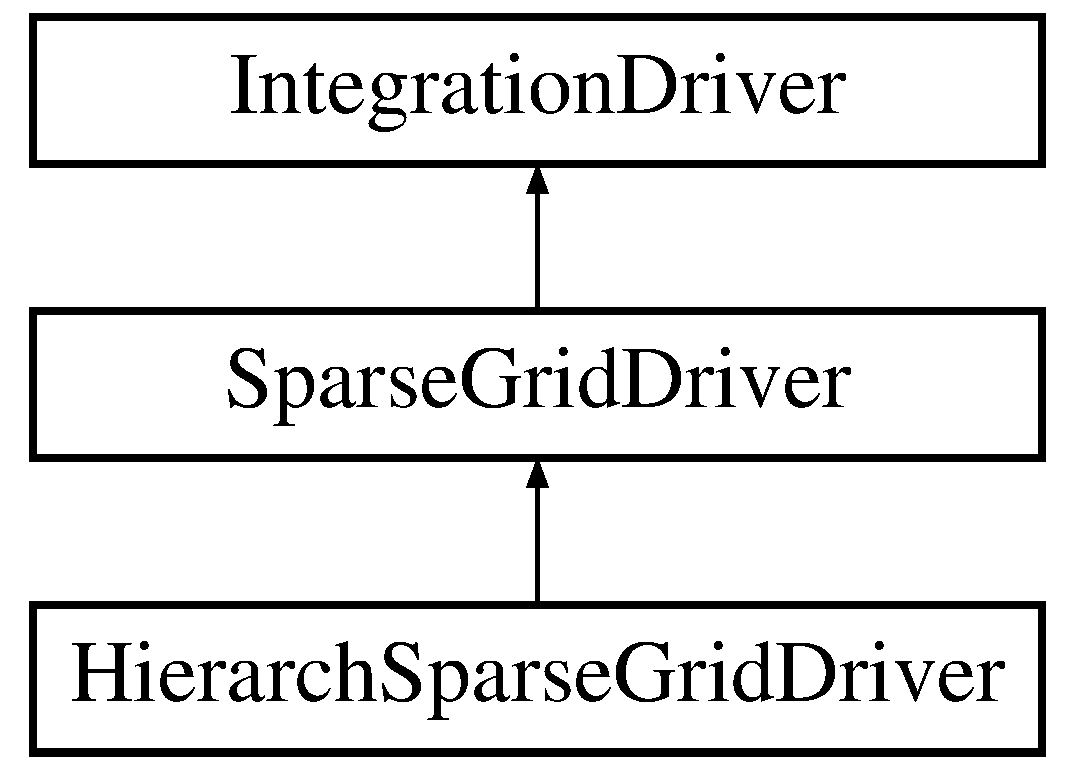
\includegraphics[height=3.000000cm]{classPecos_1_1HierarchSparseGridDriver}
\end{center}
\end{figure}
\subsection*{Public Member Functions}
\begin{DoxyCompactItemize}
\item 
\hyperlink{classPecos_1_1HierarchSparseGridDriver_ad6a2a4e748e03e3ba2bdd345500ef4f8}{Hierarch\+Sparse\+Grid\+Driver} ()\label{classPecos_1_1HierarchSparseGridDriver_ad6a2a4e748e03e3ba2bdd345500ef4f8}

\begin{DoxyCompactList}\small\item\em default constructor \end{DoxyCompactList}\item 
\hyperlink{classPecos_1_1HierarchSparseGridDriver_acac0f069a3580f15255657c0947bcce4}{Hierarch\+Sparse\+Grid\+Driver} (unsigned short ssg\+\_\+level, const Real\+Vector \&dim\+\_\+pref=Real\+Vector(), short \hyperlink{classPecos_1_1SparseGridDriver_a6f9061513ba25c62ee7a49b0d5da42cc}{growth\+\_\+rate}=M\+O\+D\+E\+R\+A\+T\+E\+\_\+\+R\+E\+S\+T\+R\+I\+C\+T\+E\+D\+\_\+\+G\+R\+O\+W\+TH, short refine\+\_\+control=N\+O\+\_\+\+C\+O\+N\+T\+R\+OL)\label{classPecos_1_1HierarchSparseGridDriver_acac0f069a3580f15255657c0947bcce4}

\begin{DoxyCompactList}\small\item\em constructor \end{DoxyCompactList}\item 
\hyperlink{classPecos_1_1HierarchSparseGridDriver_abc8d6a084fc56fef23762fee84792e12}{$\sim$\+Hierarch\+Sparse\+Grid\+Driver} ()\label{classPecos_1_1HierarchSparseGridDriver_abc8d6a084fc56fef23762fee84792e12}

\begin{DoxyCompactList}\small\item\em destructor \end{DoxyCompactList}\item 
void \hyperlink{classPecos_1_1HierarchSparseGridDriver_a30b0bccf09758808aeb7e9ca33fae2ff}{compute\+\_\+grid} (Real\+Matrix \&var\+\_\+sets)\label{classPecos_1_1HierarchSparseGridDriver_a30b0bccf09758808aeb7e9ca33fae2ff}

\begin{DoxyCompactList}\small\item\em compute scaled variable and weight sets for the T\+PQ grid \end{DoxyCompactList}\item 
int \hyperlink{classPecos_1_1HierarchSparseGridDriver_a4b04c73f01f5eb9e6171305141eb1f73}{grid\+\_\+size} ()\label{classPecos_1_1HierarchSparseGridDriver_a4b04c73f01f5eb9e6171305141eb1f73}

\begin{DoxyCompactList}\small\item\em compute number of collocation points \end{DoxyCompactList}\item 
void \hyperlink{classPecos_1_1HierarchSparseGridDriver_aeae6e6d94a2e3e77d612eee151c77799}{store\+\_\+grid} (size\+\_\+t index=\+\_\+\+N\+P\+OS)\label{classPecos_1_1HierarchSparseGridDriver_aeae6e6d94a2e3e77d612eee151c77799}

\begin{DoxyCompactList}\small\item\em store configuration settings for the current grid before advancing to the next settings within a prescribed grid sequence (default is push\+\_\+back) \end{DoxyCompactList}\item 
void \hyperlink{classPecos_1_1HierarchSparseGridDriver_a31ba839ff630bbc25292b448fff38a73}{restore\+\_\+grid} (size\+\_\+t index=\+\_\+\+N\+P\+OS)\label{classPecos_1_1HierarchSparseGridDriver_a31ba839ff630bbc25292b448fff38a73}

\begin{DoxyCompactList}\small\item\em restore configuration settings from a previously stored grid \end{DoxyCompactList}\item 
void \hyperlink{classPecos_1_1HierarchSparseGridDriver_a93215ecdfbc51b7c45998fa4d65fc7fd}{remove\+\_\+stored\+\_\+grid} (size\+\_\+t index=\+\_\+\+N\+P\+OS)\label{classPecos_1_1HierarchSparseGridDriver_a93215ecdfbc51b7c45998fa4d65fc7fd}

\begin{DoxyCompactList}\small\item\em remove configuration settings for a stored grid (default is pop\+\_\+back) \end{DoxyCompactList}\item 
void \hyperlink{classPecos_1_1HierarchSparseGridDriver_ae4337960917eda26a5672e5c6afbb62a}{clear\+\_\+stored} ()\label{classPecos_1_1HierarchSparseGridDriver_ae4337960917eda26a5672e5c6afbb62a}

\begin{DoxyCompactList}\small\item\em clear stored grid settings following their usage/combination \end{DoxyCompactList}\item 
size\+\_\+t \hyperlink{classPecos_1_1HierarchSparseGridDriver_a6edda8aad31eb8a64e180e6a76a6e0e9}{maximal\+\_\+grid} () const \label{classPecos_1_1HierarchSparseGridDriver_a6edda8aad31eb8a64e180e6a76a6e0e9}

\begin{DoxyCompactList}\small\item\em return the index of the maximal stored grid state (\+\_\+\+N\+P\+OS if the current unstored grid state) \end{DoxyCompactList}\item 
void \hyperlink{classPecos_1_1HierarchSparseGridDriver_ae42d43e21fe55d5b6cca7edf86e54818}{swap\+\_\+grid} (size\+\_\+t index)\label{classPecos_1_1HierarchSparseGridDriver_ae42d43e21fe55d5b6cca7edf86e54818}

\begin{DoxyCompactList}\small\item\em swap settings between the current grid and the stored grid identified by index \end{DoxyCompactList}\item 
void \hyperlink{classPecos_1_1HierarchSparseGridDriver_a059e9e1e03a5cd29771d369b76311261}{initialize\+\_\+sets} ()\label{classPecos_1_1HierarchSparseGridDriver_a059e9e1e03a5cd29771d369b76311261}

\begin{DoxyCompactList}\small\item\em initializes old/active/evaluation sets for use within the generalized sparse grid procedure \end{DoxyCompactList}\item 
void \hyperlink{classPecos_1_1HierarchSparseGridDriver_a99c17efb3a8e873b7708652cc1787370}{push\+\_\+trial\+\_\+set} (const U\+Short\+Array \&set)\label{classPecos_1_1HierarchSparseGridDriver_a99c17efb3a8e873b7708652cc1787370}

\begin{DoxyCompactList}\small\item\em update smolyak\+Multi\+Index with a new trial set for use within the generalized sparse grid procedure \end{DoxyCompactList}\item 
void \hyperlink{classPecos_1_1HierarchSparseGridDriver_ad9648693eacbe856825d2c78b73a3301}{restore\+\_\+set} ()\label{classPecos_1_1HierarchSparseGridDriver_ad9648693eacbe856825d2c78b73a3301}

\begin{DoxyCompactList}\small\item\em update colloc\+Key, colloc\+Indices, and unique\+Index\+Mapping based on restoration of previous trial to smolyak\+Multi\+Index \end{DoxyCompactList}\item 
void \hyperlink{classPecos_1_1HierarchSparseGridDriver_a392163a55c3c5c2b4357b5490009df62}{compute\+\_\+trial\+\_\+grid} (Real\+Matrix \&var\+\_\+sets)\label{classPecos_1_1HierarchSparseGridDriver_a392163a55c3c5c2b4357b5490009df62}

\begin{DoxyCompactList}\small\item\em computes the tensor grid for the index set from \hyperlink{classPecos_1_1HierarchSparseGridDriver_a99c17efb3a8e873b7708652cc1787370}{push\+\_\+trial\+\_\+set()} \end{DoxyCompactList}\item 
void \hyperlink{classPecos_1_1HierarchSparseGridDriver_a92b2604a79028bec35c176aee27e56bb}{pop\+\_\+trial\+\_\+set} ()\label{classPecos_1_1HierarchSparseGridDriver_a92b2604a79028bec35c176aee27e56bb}

\begin{DoxyCompactList}\small\item\em remove the previously pushed trial set from smolyak\+Multi\+Index during the course of the generalized sparse grid procedure \end{DoxyCompactList}\item 
void \hyperlink{classPecos_1_1HierarchSparseGridDriver_a07e01bf89eb07535ea78132b8d533088}{finalize\+\_\+sets} (bool output\+\_\+sets, bool converged\+\_\+within\+\_\+tol)\label{classPecos_1_1HierarchSparseGridDriver_a07e01bf89eb07535ea78132b8d533088}

\begin{DoxyCompactList}\small\item\em accept all remaining trial sets within the generalized sparse grid procedure \end{DoxyCompactList}\item 
const U\+Short\+Array \& \hyperlink{classPecos_1_1HierarchSparseGridDriver_a5c92e49dbfbcfa5b0d1523ed254b4d76}{trial\+\_\+set} () const \label{classPecos_1_1HierarchSparseGridDriver_a5c92e49dbfbcfa5b0d1523ed254b4d76}

\begin{DoxyCompactList}\small\item\em return the trial index set from \hyperlink{classPecos_1_1HierarchSparseGridDriver_a99c17efb3a8e873b7708652cc1787370}{push\+\_\+trial\+\_\+set()} \end{DoxyCompactList}\item 
int \hyperlink{classPecos_1_1HierarchSparseGridDriver_a3d8e458c7cf95eae26aa53a738844d89}{unique\+\_\+trial\+\_\+points} () const \label{classPecos_1_1HierarchSparseGridDriver_a3d8e458c7cf95eae26aa53a738844d89}

\begin{DoxyCompactList}\small\item\em return the number of unique collocation points in the trial index set \end{DoxyCompactList}\item 
void \hyperlink{classPecos_1_1HierarchSparseGridDriver_af2bf445b9a8d1f418dc3519a3305b05f}{compute\+\_\+grid\+\_\+increment} (Real\+Matrix \&var\+\_\+sets)\label{classPecos_1_1HierarchSparseGridDriver_af2bf445b9a8d1f418dc3519a3305b05f}

\begin{DoxyCompactList}\small\item\em computes tensor grids for new index sets due to an isotropic/anisotropic refinement \end{DoxyCompactList}\item 
void \hyperlink{classPecos_1_1HierarchSparseGridDriver_ae5bcc14a0e7bb726d5280c3dd10e6c98}{print\+\_\+smolyak\+\_\+multi\+\_\+index} () const \label{classPecos_1_1HierarchSparseGridDriver_ae5bcc14a0e7bb726d5280c3dd10e6c98}

\begin{DoxyCompactList}\small\item\em print smolyak\+Multi\+Index \end{DoxyCompactList}\item 
U\+Short\+U\+Short\+Pair {\bfseries level\+\_\+to\+\_\+delta\+\_\+pair} (size\+\_\+t i, unsigned short lev\+\_\+i)\label{classPecos_1_1HierarchSparseGridDriver_a848901ff3e8ea724fc2a7d114ce51ab2}

\item 
unsigned short {\bfseries level\+\_\+to\+\_\+delta\+\_\+size} (size\+\_\+t i, unsigned short lev\+\_\+i)\label{classPecos_1_1HierarchSparseGridDriver_a79cf86a8d2bf6874eb9654655c8e1236}

\item 
void {\bfseries level\+\_\+to\+\_\+delta\+\_\+key} (size\+\_\+t i, unsigned short lev\+\_\+i, U\+Short\+Array \&delta\+\_\+key\+\_\+i)\label{classPecos_1_1HierarchSparseGridDriver_ad28e1cd919d12b221e24c25a710ad91e}

\item 
void \hyperlink{classPecos_1_1HierarchSparseGridDriver_ac3ee15acadcdde2296dc77ecd10e94cb}{levels\+\_\+to\+\_\+delta\+\_\+keys} (const U\+Short\+Array \&levels, U\+Short2\+D\+Array \&delta\+\_\+keys)\label{classPecos_1_1HierarchSparseGridDriver_ac3ee15acadcdde2296dc77ecd10e94cb}

\begin{DoxyCompactList}\small\item\em convert a Smolyak index set into hierarchical quadrature keys \end{DoxyCompactList}\item 
void \hyperlink{classPecos_1_1HierarchSparseGridDriver_aa05285153ce9897c4a1815e5db24027a}{levels\+\_\+to\+\_\+delta\+\_\+sizes} (const U\+Short\+Array \&levels, U\+Short\+Array \&delta\+\_\+sizes)\label{classPecos_1_1HierarchSparseGridDriver_aa05285153ce9897c4a1815e5db24027a}

\begin{DoxyCompactList}\small\item\em convert a Smolyak index set into the sizes of hierarchical quadrature increments \end{DoxyCompactList}\item 
void \hyperlink{classPecos_1_1HierarchSparseGridDriver_a83a702e16bb1f910c689b0778f242588}{initialize\+\_\+grid} (unsigned short ssg\+\_\+level, const Real\+Vector \&dim\+\_\+pref, const Short\+Array \&u\+\_\+types, const \hyperlink{classPecos_1_1ExpansionConfigOptions}{Expansion\+Config\+Options} \&ec\+\_\+options, \hyperlink{classPecos_1_1BasisConfigOptions}{Basis\+Config\+Options} \&bc\+\_\+options, short \hyperlink{classPecos_1_1SparseGridDriver_a6f9061513ba25c62ee7a49b0d5da42cc}{growth\+\_\+rate}=M\+O\+D\+E\+R\+A\+T\+E\+\_\+\+R\+E\+S\+T\+R\+I\+C\+T\+E\+D\+\_\+\+G\+R\+O\+W\+TH, bool track\+\_\+colloc\+\_\+indices=true)\label{classPecos_1_1HierarchSparseGridDriver_a83a702e16bb1f910c689b0778f242588}

\begin{DoxyCompactList}\small\item\em initialize all sparse grid settings except for distribution params \end{DoxyCompactList}\item 
const U\+Short\+Array \& \hyperlink{classPecos_1_1HierarchSparseGridDriver_a519ca966ef4e784c01698731201e042a}{increment\+\_\+sets} () const \label{classPecos_1_1HierarchSparseGridDriver_a519ca966ef4e784c01698731201e042a}

\begin{DoxyCompactList}\small\item\em return increment\+Sets \end{DoxyCompactList}\item 
const U\+Short3\+D\+Array \& \hyperlink{classPecos_1_1HierarchSparseGridDriver_a319b6d1acf6169cf597ebfd6aca3dd08}{smolyak\+\_\+multi\+\_\+index} () const \label{classPecos_1_1HierarchSparseGridDriver_a319b6d1acf6169cf597ebfd6aca3dd08}

\begin{DoxyCompactList}\small\item\em return smolyak\+Multi\+Index \end{DoxyCompactList}\item 
void \hyperlink{classPecos_1_1HierarchSparseGridDriver_a2dd6028a82c1ac53ec629162e9edfea0}{track\+\_\+collocation\+\_\+indices} (bool track\+\_\+colloc\+\_\+indices)\label{classPecos_1_1HierarchSparseGridDriver_a2dd6028a82c1ac53ec629162e9edfea0}

\begin{DoxyCompactList}\small\item\em set track\+Colloc\+Indices \end{DoxyCompactList}\item 
bool \hyperlink{classPecos_1_1HierarchSparseGridDriver_a7d9947e97cdab5d7f3e1855e663a020d}{track\+\_\+collocation\+\_\+indices} () const \label{classPecos_1_1HierarchSparseGridDriver_a7d9947e97cdab5d7f3e1855e663a020d}

\begin{DoxyCompactList}\small\item\em get track\+Colloc\+Indices \end{DoxyCompactList}\item 
const U\+Short4\+D\+Array \& \hyperlink{classPecos_1_1HierarchSparseGridDriver_a36d15989b38fc5460654d6ce1c605998}{collocation\+\_\+key} () const \label{classPecos_1_1HierarchSparseGridDriver_a36d15989b38fc5460654d6ce1c605998}

\begin{DoxyCompactList}\small\item\em return colloc\+Key \end{DoxyCompactList}\item 
const Sizet3\+D\+Array \& \hyperlink{classPecos_1_1HierarchSparseGridDriver_a2422d7adf5fccacbc664189508f03022}{collocation\+\_\+indices} () const \label{classPecos_1_1HierarchSparseGridDriver_a2422d7adf5fccacbc664189508f03022}

\begin{DoxyCompactList}\small\item\em return colloc\+Indices \end{DoxyCompactList}\item 
const U\+Short3\+D\+Array \& \hyperlink{classPecos_1_1HierarchSparseGridDriver_a4477fb6676f396ab83aa198fe0331bea}{stored\+\_\+smolyak\+\_\+multi\+\_\+index} (size\+\_\+t index) const \label{classPecos_1_1HierarchSparseGridDriver_a4477fb6676f396ab83aa198fe0331bea}

\begin{DoxyCompactList}\small\item\em return stored\+Lev\+Multi\+Index \end{DoxyCompactList}\item 
const U\+Short4\+D\+Array \& \hyperlink{classPecos_1_1HierarchSparseGridDriver_a03ca3eb80aa3d844b7da9253cf2a2cca}{stored\+\_\+collocation\+\_\+key} (size\+\_\+t index) const \label{classPecos_1_1HierarchSparseGridDriver_a03ca3eb80aa3d844b7da9253cf2a2cca}

\begin{DoxyCompactList}\small\item\em return stored\+Colloc\+Key \end{DoxyCompactList}\item 
void \hyperlink{classPecos_1_1HierarchSparseGridDriver_a490283a942bdcd3be233d62f6bd6049b}{partition\+\_\+keys} (U\+Short2\+D\+Array \&reference\+\_\+set\+\_\+range, U\+Short2\+D\+Array \&increment\+\_\+set\+\_\+range) const \label{classPecos_1_1HierarchSparseGridDriver_a490283a942bdcd3be233d62f6bd6049b}

\begin{DoxyCompactList}\small\item\em discriminate portions of the level-\/set hierarchy that are reference sets from those in the current increment \end{DoxyCompactList}\item 
void \hyperlink{classPecos_1_1HierarchSparseGridDriver_a3f4e05177766404f7144267d11827730}{partition\+\_\+keys} (U\+Short3\+D\+Array \&reference\+\_\+pt\+\_\+range, U\+Short3\+D\+Array \&increment\+\_\+pt\+\_\+range) const \label{classPecos_1_1HierarchSparseGridDriver_a3f4e05177766404f7144267d11827730}

\begin{DoxyCompactList}\small\item\em discriminate portions of the level-\/set-\/point hierarchy that are in the reference grid from those in the current increment \end{DoxyCompactList}\item 
const Real\+Vector2\+D\+Array \& \hyperlink{classPecos_1_1HierarchSparseGridDriver_aeff94c7a8a4c656d3817c5e6b7a5f270}{type1\+\_\+weight\+\_\+set\+\_\+arrays} () const \label{classPecos_1_1HierarchSparseGridDriver_aeff94c7a8a4c656d3817c5e6b7a5f270}

\begin{DoxyCompactList}\small\item\em return type1\+Weight\+Sets for use in hierarchical integration functions \end{DoxyCompactList}\item 
const Real\+Matrix2\+D\+Array \& \hyperlink{classPecos_1_1HierarchSparseGridDriver_a320a9c7281ba87d1c1795ba96720fc08}{type2\+\_\+weight\+\_\+set\+\_\+arrays} () const \label{classPecos_1_1HierarchSparseGridDriver_a320a9c7281ba87d1c1795ba96720fc08}

\begin{DoxyCompactList}\small\item\em return type2\+Weight\+Sets for use in hierarchical integration functions \end{DoxyCompactList}\end{DoxyCompactItemize}
\subsection*{Private Member Functions}
\begin{DoxyCompactItemize}
\item 
void {\bfseries update\+\_\+smolyak\+\_\+multi\+\_\+index} (bool clear\+\_\+sm\+\_\+mi=false)\label{classPecos_1_1HierarchSparseGridDriver_a548500f3592c3016a5c9f9158116dd45}

\item 
void {\bfseries assign\+\_\+collocation\+\_\+key} ()\label{classPecos_1_1HierarchSparseGridDriver_a9d17415950cab71229a9e2968121ff22}

\item 
void {\bfseries update\+\_\+collocation\+\_\+key} ()\label{classPecos_1_1HierarchSparseGridDriver_aa0afe77dc7d6ec1b1335b59429701e52}

\item 
void {\bfseries assign\+\_\+collocation\+\_\+indices} ()\label{classPecos_1_1HierarchSparseGridDriver_ad9e72cee34135fb982921365ccd615cd}

\item 
void {\bfseries update\+\_\+collocation\+\_\+indices} ()\label{classPecos_1_1HierarchSparseGridDriver_a280d7a1ff687e24bc8d27bc926ee11da}

\item 
void \hyperlink{classPecos_1_1HierarchSparseGridDriver_a09ad9a025482d9417274ed0a19afca8e}{compute\+\_\+points\+\_\+weights} (Real\+Matrix \&pts, Real\+Vector \&t1\+\_\+wts, Real\+Matrix \&t2\+\_\+wts, const U\+Short\+Array \&sm\+\_\+index, const U\+Short2\+D\+Array \&colloc\+\_\+key)\label{classPecos_1_1HierarchSparseGridDriver_a09ad9a025482d9417274ed0a19afca8e}

\begin{DoxyCompactList}\small\item\em kernel routine used for trial set and full sparse grid computations \end{DoxyCompactList}\item 
void \hyperlink{classPecos_1_1HierarchSparseGridDriver_aa034123d6d3477efb156ba1c8add03a9}{compute\+\_\+points\+\_\+weights} (Real\+Matrix \&pts, Real\+Vector \&t1\+\_\+wts, Real\+Matrix \&t2\+\_\+wts)\label{classPecos_1_1HierarchSparseGridDriver_aa034123d6d3477efb156ba1c8add03a9}

\begin{DoxyCompactList}\small\item\em compute points and weights for a trial set \end{DoxyCompactList}\item 
void \hyperlink{classPecos_1_1HierarchSparseGridDriver_a32c1b2db7b05e83d49b266876e9773ff}{compute\+\_\+points\+\_\+weights} (Real\+Matrix \&pts, Real\+Vector2\+D\+Array \&t1\+\_\+wts, Real\+Matrix2\+D\+Array \&t2\+\_\+wts)
\begin{DoxyCompactList}\small\item\em compute points and weights for all levels of the (initial) sparse grid \end{DoxyCompactList}\end{DoxyCompactItemize}
\subsection*{Private Attributes}
\begin{DoxyCompactItemize}
\item 
bool \hyperlink{classPecos_1_1HierarchSparseGridDriver_a89ccad2f5ea68ce90e10140ba64cbd2b}{nested\+Grid}\label{classPecos_1_1HierarchSparseGridDriver_a89ccad2f5ea68ce90e10140ba64cbd2b}

\begin{DoxyCompactList}\small\item\em flag for use of fully nested 1D rules, allowing formulation using collocation point increments \end{DoxyCompactList}\item 
U\+Short3\+D\+Array \hyperlink{classPecos_1_1HierarchSparseGridDriver_a1899fc99ce06e7d1dab0c21445725cba}{smolyak\+Multi\+Index}
\begin{DoxyCompactList}\small\item\em interpolation depth by index set by num\+Vars array for identifying the index to use within the polynomial\+Basis for a particular variable \end{DoxyCompactList}\item 
unsigned short \hyperlink{classPecos_1_1HierarchSparseGridDriver_a69e006a77c0dcbba4d6784d0678a137c}{trial\+Level}\label{classPecos_1_1HierarchSparseGridDriver_a69e006a77c0dcbba4d6784d0678a137c}

\begin{DoxyCompactList}\small\item\em level of trial evaluation set from \hyperlink{classPecos_1_1HierarchSparseGridDriver_a99c17efb3a8e873b7708652cc1787370}{push\+\_\+trial\+\_\+set()}; trial set corresponds to smolyak\+Multi\+Index\mbox{[}trial\+Level\mbox{]}.back() \end{DoxyCompactList}\item 
U\+Short\+Array \hyperlink{classPecos_1_1HierarchSparseGridDriver_a36e2466de81a49ee32105f49eda11573}{increment\+Sets}\label{classPecos_1_1HierarchSparseGridDriver_a36e2466de81a49ee32105f49eda11573}

\begin{DoxyCompactList}\small\item\em identifies the trailing index set increments within smolyak\+Multi\+Index due to an isotropic/anistropic grid refinement \end{DoxyCompactList}\item 
bool \hyperlink{classPecos_1_1HierarchSparseGridDriver_a277523d2de6de32b78ab32f0e4d24e9f}{track\+Colloc\+Indices}\label{classPecos_1_1HierarchSparseGridDriver_a277523d2de6de32b78ab32f0e4d24e9f}

\begin{DoxyCompactList}\small\item\em due to the hierarchical structure, collocation indices only need to be defined in special cases (e.\+g., generalized sparse grids for which index sets can appear in different orders). \end{DoxyCompactList}\item 
U\+Short4\+D\+Array \hyperlink{classPecos_1_1HierarchSparseGridDriver_a7cbbd68b6b4e7320cb28a5e4b8894f52}{colloc\+Key}\label{classPecos_1_1HierarchSparseGridDriver_a7cbbd68b6b4e7320cb28a5e4b8894f52}

\begin{DoxyCompactList}\small\item\em levels-\/by-\/index sets-\/by-\/num\+Delta\+Pts-\/by-\/num\+Vars array for identifying the 1-\/D point indices for sets of tensor-\/product collocation points \end{DoxyCompactList}\item 
Sizet3\+D\+Array \hyperlink{classPecos_1_1HierarchSparseGridDriver_a9d5321a039a785dbc50d99212c18325c}{colloc\+Indices}\label{classPecos_1_1HierarchSparseGridDriver_a9d5321a039a785dbc50d99212c18325c}

\begin{DoxyCompactList}\small\item\em levels-\/by-\/index sets-\/by-\/num\+Tensor\+Product\+Pts array for linking the set of tensor products to the unique collocation points evaluated \end{DoxyCompactList}\item 
U\+Short4\+D\+Array \hyperlink{classPecos_1_1HierarchSparseGridDriver_a1bd8eb5cffea6b67f167ed179b36157e}{stored\+Lev\+Multi\+Index}\label{classPecos_1_1HierarchSparseGridDriver_a1bd8eb5cffea6b67f167ed179b36157e}

\begin{DoxyCompactList}\small\item\em stored driver states\+: copies of smolyak\+Multi\+Index \end{DoxyCompactList}\item 
U\+Short5\+D\+Array \hyperlink{classPecos_1_1HierarchSparseGridDriver_a686a8fd6e3090a7667c95d0a8d6c84da}{stored\+Colloc\+Key}\label{classPecos_1_1HierarchSparseGridDriver_a686a8fd6e3090a7667c95d0a8d6c84da}

\begin{DoxyCompactList}\small\item\em stored driver states\+: copies of colloc\+Key \end{DoxyCompactList}\item 
Real\+Vector2\+D\+Array \hyperlink{classPecos_1_1HierarchSparseGridDriver_a5de56b20e57fb8bb96f62e06de1e9ea3}{type1\+Weight\+Sets}\label{classPecos_1_1HierarchSparseGridDriver_a5de56b20e57fb8bb96f62e06de1e9ea3}

\begin{DoxyCompactList}\small\item\em the set of type1 weights (for integration of value interpolants) associated with each point in the sparse grid \end{DoxyCompactList}\item 
Real\+Matrix2\+D\+Array \hyperlink{classPecos_1_1HierarchSparseGridDriver_abdaca2cdf2efec3b6b5af2d9adc04a54}{type2\+Weight\+Sets}\label{classPecos_1_1HierarchSparseGridDriver_abdaca2cdf2efec3b6b5af2d9adc04a54}

\begin{DoxyCompactList}\small\item\em the set of type2 weights (for integration of gradient interpolants) for each derivative component and for each point in the sparse grid \end{DoxyCompactList}\item 
Real\+Vector3\+D\+Array \hyperlink{classPecos_1_1HierarchSparseGridDriver_ac4aeabf6ae4069caa0608b5f1c0be43d}{stored\+Type1\+Weight\+Sets}\label{classPecos_1_1HierarchSparseGridDriver_ac4aeabf6ae4069caa0608b5f1c0be43d}

\begin{DoxyCompactList}\small\item\em stored driver state\+: copy of type1\+Weight\+Sets \end{DoxyCompactList}\item 
Real\+Matrix3\+D\+Array \hyperlink{classPecos_1_1HierarchSparseGridDriver_a8e2675de76cb8b6db1efe3375ba408a1}{stored\+Type2\+Weight\+Sets}\label{classPecos_1_1HierarchSparseGridDriver_a8e2675de76cb8b6db1efe3375ba408a1}

\begin{DoxyCompactList}\small\item\em stored driver state\+: copy of type2\+Weight\+Sets \end{DoxyCompactList}\item 
std\+::map$<$ U\+Short\+Array, Real\+Vector $>$ \hyperlink{classPecos_1_1HierarchSparseGridDriver_adacb7309f3bcc04193e19e0f673d491f}{popped\+T1\+Wt\+Sets}\label{classPecos_1_1HierarchSparseGridDriver_adacb7309f3bcc04193e19e0f673d491f}

\begin{DoxyCompactList}\small\item\em type 1 weight sets popped during decrement for later restoration to type1\+Weight\+Sets \end{DoxyCompactList}\item 
std\+::map$<$ U\+Short\+Array, Real\+Matrix $>$ \hyperlink{classPecos_1_1HierarchSparseGridDriver_a76484c1349edf58640be2caa82d99a66}{popped\+T2\+Wt\+Sets}\label{classPecos_1_1HierarchSparseGridDriver_a76484c1349edf58640be2caa82d99a66}

\begin{DoxyCompactList}\small\item\em type 2 weight sets popped during decrement for later restoration to type2\+Weight\+Sets \end{DoxyCompactList}\end{DoxyCompactItemize}
\subsection*{Additional Inherited Members}


\subsection{Detailed Description}
Derived integration driver class that generates N-\/dimensional Smolyak sparse grids for numerical evaluation of expectation integrals over independent standard random variables. 

This class is used by Dakota\+::\+Non\+D\+Sparse\+Grid, but could also be used for general numerical integration of moments. It employs 1-\/D Clenshaw-\/\+Curtis, Newton-\/\+Cotes, and Gaussian quadrature rules within Smolyak sparse grids. 

\subsection{Member Function Documentation}
\index{Pecos\+::\+Hierarch\+Sparse\+Grid\+Driver@{Pecos\+::\+Hierarch\+Sparse\+Grid\+Driver}!compute\+\_\+points\+\_\+weights@{compute\+\_\+points\+\_\+weights}}
\index{compute\+\_\+points\+\_\+weights@{compute\+\_\+points\+\_\+weights}!Pecos\+::\+Hierarch\+Sparse\+Grid\+Driver@{Pecos\+::\+Hierarch\+Sparse\+Grid\+Driver}}
\subsubsection[{\texorpdfstring{compute\+\_\+points\+\_\+weights(\+Real\+Matrix \&pts, Real\+Vector2\+D\+Array \&t1\+\_\+wts, Real\+Matrix2\+D\+Array \&t2\+\_\+wts)}{compute_points_weights(RealMatrix &pts, RealVector2DArray &t1_wts, RealMatrix2DArray &t2_wts)}}]{\setlength{\rightskip}{0pt plus 5cm}void compute\+\_\+points\+\_\+weights (
\begin{DoxyParamCaption}
\item[{Real\+Matrix \&}]{pts, }
\item[{Real\+Vector2\+D\+Array \&}]{t1\+\_\+wts, }
\item[{Real\+Matrix2\+D\+Array \&}]{t2\+\_\+wts}
\end{DoxyParamCaption}
)\hspace{0.3cm}{\ttfamily [private]}}\label{classPecos_1_1HierarchSparseGridDriver_a32c1b2db7b05e83d49b266876e9773ff}


compute points and weights for all levels of the (initial) sparse grid 

Points are collapsed as required for compute\+\_\+grid(var\+\_\+sets), but t1/t2 weights are hierarchical 2D arrays. 

References Hierarch\+Sparse\+Grid\+Driver\+::colloc\+Key, Hierarch\+Sparse\+Grid\+Driver\+::compute\+\_\+points\+\_\+weights(), Integration\+Driver\+::num\+Vars, and Hierarch\+Sparse\+Grid\+Driver\+::smolyak\+Multi\+Index.



\subsection{Member Data Documentation}
\index{Pecos\+::\+Hierarch\+Sparse\+Grid\+Driver@{Pecos\+::\+Hierarch\+Sparse\+Grid\+Driver}!smolyak\+Multi\+Index@{smolyak\+Multi\+Index}}
\index{smolyak\+Multi\+Index@{smolyak\+Multi\+Index}!Pecos\+::\+Hierarch\+Sparse\+Grid\+Driver@{Pecos\+::\+Hierarch\+Sparse\+Grid\+Driver}}
\subsubsection[{\texorpdfstring{smolyak\+Multi\+Index}{smolyakMultiIndex}}]{\setlength{\rightskip}{0pt plus 5cm}U\+Short3\+D\+Array smolyak\+Multi\+Index\hspace{0.3cm}{\ttfamily [private]}}\label{classPecos_1_1HierarchSparseGridDriver_a1899fc99ce06e7d1dab0c21445725cba}


interpolation depth by index set by num\+Vars array for identifying the index to use within the polynomial\+Basis for a particular variable 

The index sets correspond to j (0-\/based) for use as indices, which are offset from the i indices (1-\/based) normally used in the Smolyak expressions. The indices correspond to levels, one within each anisotropic tensor-\/product integration of a Smolyak recursion. 

Referenced by Hierarch\+Sparse\+Grid\+Driver\+::compute\+\_\+grid\+\_\+increment(), Hierarch\+Sparse\+Grid\+Driver\+::compute\+\_\+points\+\_\+weights(), Hierarch\+Sparse\+Grid\+Driver\+::finalize\+\_\+sets(), Hierarch\+Sparse\+Grid\+Driver\+::grid\+\_\+size(), Hierarch\+Sparse\+Grid\+Driver\+::initialize\+\_\+sets(), Hierarch\+Sparse\+Grid\+Driver\+::partition\+\_\+keys(), Hierarch\+Sparse\+Grid\+Driver\+::pop\+\_\+trial\+\_\+set(), Hierarch\+Sparse\+Grid\+Driver\+::print\+\_\+smolyak\+\_\+multi\+\_\+index(), Hierarch\+Sparse\+Grid\+Driver\+::push\+\_\+trial\+\_\+set(), Hierarch\+Sparse\+Grid\+Driver\+::restore\+\_\+grid(), Hierarch\+Sparse\+Grid\+Driver\+::smolyak\+\_\+multi\+\_\+index(), Hierarch\+Sparse\+Grid\+Driver\+::store\+\_\+grid(), Hierarch\+Sparse\+Grid\+Driver\+::swap\+\_\+grid(), and Hierarch\+Sparse\+Grid\+Driver\+::trial\+\_\+set().



The documentation for this class was generated from the following files\+:\begin{DoxyCompactItemize}
\item 
Hierarch\+Sparse\+Grid\+Driver.\+hpp\item 
Hierarch\+Sparse\+Grid\+Driver.\+cpp\end{DoxyCompactItemize}

\section{Histogram\+Bin\+Random\+Variable Class Reference}
\label{classPecos_1_1HistogramBinRandomVariable}\index{Histogram\+Bin\+Random\+Variable@{Histogram\+Bin\+Random\+Variable}}


Derived random variable class for gumbel random variables.  


Inheritance diagram for Histogram\+Bin\+Random\+Variable\+:\begin{figure}[H]
\begin{center}
\leavevmode
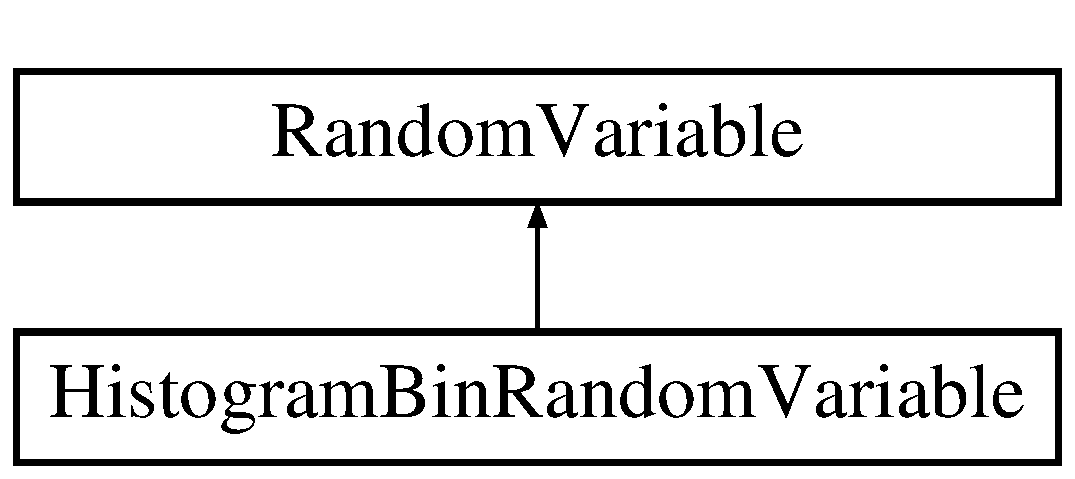
\includegraphics[height=2.000000cm]{classPecos_1_1HistogramBinRandomVariable}
\end{center}
\end{figure}
\subsection*{Public Member Functions}
\begin{DoxyCompactItemize}
\item 
\hyperlink{classPecos_1_1HistogramBinRandomVariable_ac2ab76a2a5022a6ce21d489871a8dca7}{Histogram\+Bin\+Random\+Variable} ()\label{classPecos_1_1HistogramBinRandomVariable_ac2ab76a2a5022a6ce21d489871a8dca7}

\begin{DoxyCompactList}\small\item\em default constructor \end{DoxyCompactList}\item 
\hyperlink{classPecos_1_1HistogramBinRandomVariable_a72f6f79bbd27aefba07871863f4c4ce1}{Histogram\+Bin\+Random\+Variable} (const Real\+Real\+Map \&bin\+\_\+prs)\label{classPecos_1_1HistogramBinRandomVariable_a72f6f79bbd27aefba07871863f4c4ce1}

\begin{DoxyCompactList}\small\item\em alternate constructor \end{DoxyCompactList}\item 
\hyperlink{classPecos_1_1HistogramBinRandomVariable_aea0d3b537e43d84b345d552161c3b3ca}{$\sim$\+Histogram\+Bin\+Random\+Variable} ()\label{classPecos_1_1HistogramBinRandomVariable_aea0d3b537e43d84b345d552161c3b3ca}

\begin{DoxyCompactList}\small\item\em destructor \end{DoxyCompactList}\item 
Real \hyperlink{classPecos_1_1HistogramBinRandomVariable_addd564e7f4f314e12d38df74d845f0d8}{cdf} (Real x) const \label{classPecos_1_1HistogramBinRandomVariable_addd564e7f4f314e12d38df74d845f0d8}

\begin{DoxyCompactList}\small\item\em return the cumulative distribution function value of the random variable at x \end{DoxyCompactList}\item 
Real \hyperlink{classPecos_1_1HistogramBinRandomVariable_a23c3b599e7e4788a9a5e9e93c3dbaf4d}{ccdf} (Real x) const \label{classPecos_1_1HistogramBinRandomVariable_a23c3b599e7e4788a9a5e9e93c3dbaf4d}

\begin{DoxyCompactList}\small\item\em return the complementary cumulative distribution function value of the random variable at x \end{DoxyCompactList}\item 
Real \hyperlink{classPecos_1_1HistogramBinRandomVariable_a918a1aac05ca349ea5313eebcba46c3e}{inverse\+\_\+cdf} (Real p\+\_\+cdf) const \label{classPecos_1_1HistogramBinRandomVariable_a918a1aac05ca349ea5313eebcba46c3e}

\begin{DoxyCompactList}\small\item\em return the x value corresponding to a cumulative probability \end{DoxyCompactList}\item 
Real \hyperlink{classPecos_1_1HistogramBinRandomVariable_afda003a1f59ff6930902cd5c8601f49b}{inverse\+\_\+ccdf} (Real p\+\_\+ccdf) const \label{classPecos_1_1HistogramBinRandomVariable_afda003a1f59ff6930902cd5c8601f49b}

\begin{DoxyCompactList}\small\item\em return the x value corresponding to a complementary cumulative probability \end{DoxyCompactList}\item 
Real \hyperlink{classPecos_1_1HistogramBinRandomVariable_a8ec69265f428e17c1707133cb137a819}{pdf} (Real x) const \label{classPecos_1_1HistogramBinRandomVariable_a8ec69265f428e17c1707133cb137a819}

\begin{DoxyCompactList}\small\item\em return the value of the random variable\textquotesingle{}s probability density function at x \end{DoxyCompactList}\item 
Real \hyperlink{classPecos_1_1HistogramBinRandomVariable_aaa7ca3718abc034be7629af5594efca0}{pdf\+\_\+gradient} (Real x) const \label{classPecos_1_1HistogramBinRandomVariable_aaa7ca3718abc034be7629af5594efca0}

\begin{DoxyCompactList}\small\item\em return the gradient of the random variable\textquotesingle{}s probability density function at x \end{DoxyCompactList}\item 
Real \hyperlink{classPecos_1_1HistogramBinRandomVariable_a514a0abe97269ac6e003f43683d9137e}{pdf\+\_\+hessian} (Real x) const \label{classPecos_1_1HistogramBinRandomVariable_a514a0abe97269ac6e003f43683d9137e}

\begin{DoxyCompactList}\small\item\em return the hessian of the random variable\textquotesingle{}s probability density function at x \end{DoxyCompactList}\item 
Real \hyperlink{classPecos_1_1HistogramBinRandomVariable_a962ffe5a3593be370d5c883365c060f4}{mean} () const \label{classPecos_1_1HistogramBinRandomVariable_a962ffe5a3593be370d5c883365c060f4}

\begin{DoxyCompactList}\small\item\em return the distribution mean \end{DoxyCompactList}\item 
Real \hyperlink{classPecos_1_1HistogramBinRandomVariable_a72d3d6926edd929cb3f8e12baa655f70}{mode} () const \label{classPecos_1_1HistogramBinRandomVariable_a72d3d6926edd929cb3f8e12baa655f70}

\begin{DoxyCompactList}\small\item\em return the distribution mode \end{DoxyCompactList}\item 
Real \hyperlink{classPecos_1_1HistogramBinRandomVariable_a4b8b05b2a9af92dad9cc304c2925a4eb}{variance} () const \label{classPecos_1_1HistogramBinRandomVariable_a4b8b05b2a9af92dad9cc304c2925a4eb}

\begin{DoxyCompactList}\small\item\em return the distribution variance \end{DoxyCompactList}\item 
Real\+Real\+Pair \hyperlink{classPecos_1_1HistogramBinRandomVariable_a80e9024c98c6105a5eace8601a91b3d3}{moments} () const 
\begin{DoxyCompactList}\small\item\em return the distribution mean and standard deviation as a pair \end{DoxyCompactList}\item 
Real\+Real\+Pair \hyperlink{classPecos_1_1HistogramBinRandomVariable_a4bdb95a8fa5fffaa0de5102f56963cf2}{bounds} () const \label{classPecos_1_1HistogramBinRandomVariable_a4bdb95a8fa5fffaa0de5102f56963cf2}

\begin{DoxyCompactList}\small\item\em return the distribution lower and upper bounds as a pair \end{DoxyCompactList}\item 
Real \hyperlink{classPecos_1_1HistogramBinRandomVariable_ae1cf1c07047d7ad9dbb899aa01138d54}{coefficient\+\_\+of\+\_\+variation} () const 
\begin{DoxyCompactList}\small\item\em compute the coefficient of variation (used to compute selected correlation warping factors); defined for semi-\/infinite distributions with nonzero mean (lognormal, exponential, gamma, frechet, weibull) \end{DoxyCompactList}\item 
void {\bfseries update} (const Real\+Real\+Map \&bin\+\_\+prs)\label{classPecos_1_1HistogramBinRandomVariable_ae090ed665f667266b706e11c3b561043}

\end{DoxyCompactItemize}
\subsection*{Static Public Member Functions}
\begin{DoxyCompactItemize}
\item 
static Real {\bfseries pdf} (Real x, const Real\+Real\+Map \&bin\+\_\+prs)\label{classPecos_1_1HistogramBinRandomVariable_aa78e445e8071ed1e8da12de52cdbefb3}

\item 
static Real {\bfseries cdf} (Real x, const Real\+Real\+Map \&bin\+\_\+prs)\label{classPecos_1_1HistogramBinRandomVariable_a9f6e7cb49835bf9275856220e2919c30}

\item 
static Real {\bfseries inverse\+\_\+cdf} (Real \hyperlink{classPecos_1_1HistogramBinRandomVariable_addd564e7f4f314e12d38df74d845f0d8}{cdf}, const Real\+Real\+Map \&bin\+\_\+prs)\label{classPecos_1_1HistogramBinRandomVariable_a40a7d7fbd48653bde304ea050fc6ce25}

\item 
static Real {\bfseries pdf} (Real x, const Real\+Vector \&bin\+\_\+prs)\label{classPecos_1_1HistogramBinRandomVariable_ae5f1970871762a513b64975d05b9f851}

\item 
static Real {\bfseries cdf} (Real x, const Real\+Vector \&bin\+\_\+prs)\label{classPecos_1_1HistogramBinRandomVariable_a032c9f2aa0c5b962f0600c23b0928827}

\item 
static Real {\bfseries inverse\+\_\+cdf} (Real \hyperlink{classPecos_1_1HistogramBinRandomVariable_addd564e7f4f314e12d38df74d845f0d8}{cdf}, const Real\+Vector \&bin\+\_\+prs)\label{classPecos_1_1HistogramBinRandomVariable_af22e3710ee3c47c45b430c16efe1e9bc}

\item 
static void {\bfseries moments\+\_\+from\+\_\+params} (const Real\+Real\+Map \&bin\+\_\+prs, Real \&\hyperlink{classPecos_1_1HistogramBinRandomVariable_a962ffe5a3593be370d5c883365c060f4}{mean}, Real \&std\+\_\+dev)\label{classPecos_1_1HistogramBinRandomVariable_af727d65dc707ee958179edcf85b9df5c}

\end{DoxyCompactItemize}
\subsection*{Protected Attributes}
\begin{DoxyCompactItemize}
\item 
Real\+Real\+Map \hyperlink{classPecos_1_1HistogramBinRandomVariable_a3abb5d3b3e536de19f768ff1072e3aa1}{bin\+Pairs}\label{classPecos_1_1HistogramBinRandomVariable_a3abb5d3b3e536de19f768ff1072e3aa1}

\begin{DoxyCompactList}\small\item\em pairings of abscissas to bin counts \end{DoxyCompactList}\end{DoxyCompactItemize}
\subsection*{Additional Inherited Members}


\subsection{Detailed Description}
Derived random variable class for gumbel random variables. 

Manages the bin\+Pairs mapping. 

\subsection{Member Function Documentation}
\index{Pecos\+::\+Histogram\+Bin\+Random\+Variable@{Pecos\+::\+Histogram\+Bin\+Random\+Variable}!moments@{moments}}
\index{moments@{moments}!Pecos\+::\+Histogram\+Bin\+Random\+Variable@{Pecos\+::\+Histogram\+Bin\+Random\+Variable}}
\subsubsection[{\texorpdfstring{moments() const }{moments() const }}]{\setlength{\rightskip}{0pt plus 5cm}Real\+Real\+Pair moments (
\begin{DoxyParamCaption}
{}
\end{DoxyParamCaption}
) const\hspace{0.3cm}{\ttfamily [inline]}, {\ttfamily [virtual]}}\label{classPecos_1_1HistogramBinRandomVariable_a80e9024c98c6105a5eace8601a91b3d3}


return the distribution mean and standard deviation as a pair 

default is only overridden when more efficient to compute together 

Reimplemented from \hyperlink{classPecos_1_1RandomVariable_a80e9024c98c6105a5eace8601a91b3d3}{Random\+Variable}.



References Histogram\+Bin\+Random\+Variable\+::bin\+Pairs, and Histogram\+Bin\+Random\+Variable\+::mean().

\index{Pecos\+::\+Histogram\+Bin\+Random\+Variable@{Pecos\+::\+Histogram\+Bin\+Random\+Variable}!coefficient\+\_\+of\+\_\+variation@{coefficient\+\_\+of\+\_\+variation}}
\index{coefficient\+\_\+of\+\_\+variation@{coefficient\+\_\+of\+\_\+variation}!Pecos\+::\+Histogram\+Bin\+Random\+Variable@{Pecos\+::\+Histogram\+Bin\+Random\+Variable}}
\subsubsection[{\texorpdfstring{coefficient\+\_\+of\+\_\+variation() const }{coefficient_of_variation() const }}]{\setlength{\rightskip}{0pt plus 5cm}Real coefficient\+\_\+of\+\_\+variation (
\begin{DoxyParamCaption}
{}
\end{DoxyParamCaption}
) const\hspace{0.3cm}{\ttfamily [inline]}, {\ttfamily [virtual]}}\label{classPecos_1_1HistogramBinRandomVariable_ae1cf1c07047d7ad9dbb899aa01138d54}


compute the coefficient of variation (used to compute selected correlation warping factors); defined for semi-\/infinite distributions with nonzero mean (lognormal, exponential, gamma, frechet, weibull) 

default is only overridden when more efficient to compute together 

Reimplemented from \hyperlink{classPecos_1_1RandomVariable_ae1cf1c07047d7ad9dbb899aa01138d54}{Random\+Variable}.



References Histogram\+Bin\+Random\+Variable\+::bin\+Pairs, Histogram\+Bin\+Random\+Variable\+::cdf(), Histogram\+Bin\+Random\+Variable\+::inverse\+\_\+cdf(), Histogram\+Bin\+Random\+Variable\+::mean(), and Histogram\+Bin\+Random\+Variable\+::pdf().



The documentation for this class was generated from the following file\+:\begin{DoxyCompactItemize}
\item 
Histogram\+Bin\+Random\+Variable.\+hpp\end{DoxyCompactItemize}

\section{Histogram\+Pt\+Random\+Variable Class Reference}
\label{classPecos_1_1HistogramPtRandomVariable}\index{Histogram\+Pt\+Random\+Variable@{Histogram\+Pt\+Random\+Variable}}


Derived random variable class for gumbel random variables.  


Inheritance diagram for Histogram\+Pt\+Random\+Variable\+:\begin{figure}[H]
\begin{center}
\leavevmode
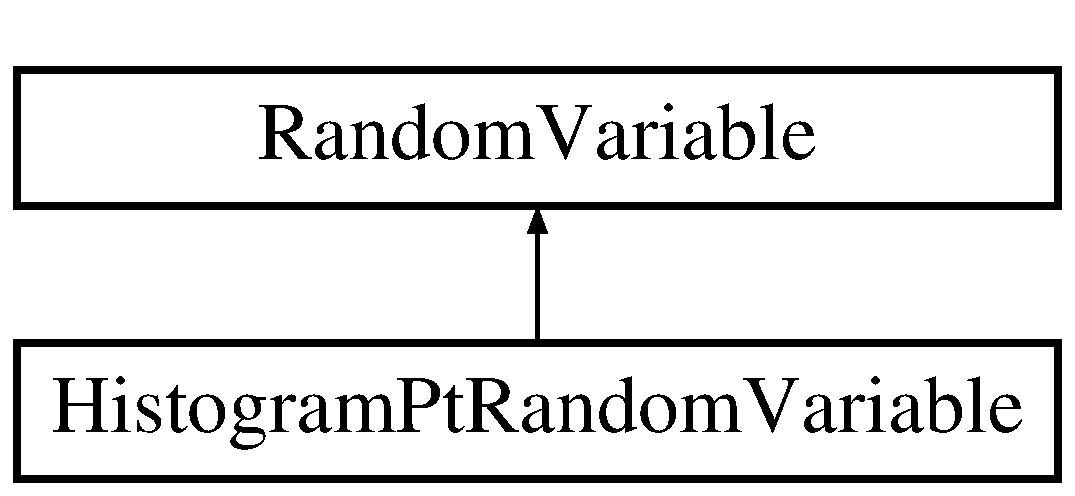
\includegraphics[height=2.000000cm]{classPecos_1_1HistogramPtRandomVariable}
\end{center}
\end{figure}
\subsection*{Public Member Functions}
\begin{DoxyCompactItemize}
\item 
\hyperlink{classPecos_1_1HistogramPtRandomVariable_a38cc5d39ce429fd42a027974fc5bd5ca}{Histogram\+Pt\+Random\+Variable} ()\label{classPecos_1_1HistogramPtRandomVariable_a38cc5d39ce429fd42a027974fc5bd5ca}

\begin{DoxyCompactList}\small\item\em default constructor \end{DoxyCompactList}\item 
\hyperlink{classPecos_1_1HistogramPtRandomVariable_a9b5daad3f441284551548a7735b931da}{Histogram\+Pt\+Random\+Variable} (const Int\+Real\+Map \&i\+\_\+prs)\label{classPecos_1_1HistogramPtRandomVariable_a9b5daad3f441284551548a7735b931da}

\begin{DoxyCompactList}\small\item\em alternate constructor \end{DoxyCompactList}\item 
\hyperlink{classPecos_1_1HistogramPtRandomVariable_aac7db4207793e67ca1fd41f0f6fcc761}{Histogram\+Pt\+Random\+Variable} (const String\+Real\+Map \&s\+\_\+prs)\label{classPecos_1_1HistogramPtRandomVariable_aac7db4207793e67ca1fd41f0f6fcc761}

\begin{DoxyCompactList}\small\item\em alternate constructor \end{DoxyCompactList}\item 
\hyperlink{classPecos_1_1HistogramPtRandomVariable_a8908dc26071d8e5f0208ac546ff6e12a}{Histogram\+Pt\+Random\+Variable} (const Real\+Real\+Map \&r\+\_\+prs)\label{classPecos_1_1HistogramPtRandomVariable_a8908dc26071d8e5f0208ac546ff6e12a}

\begin{DoxyCompactList}\small\item\em alternate constructor \end{DoxyCompactList}\item 
\hyperlink{classPecos_1_1HistogramPtRandomVariable_a80cdabb336eb027b7634a6bf02a1460d}{$\sim$\+Histogram\+Pt\+Random\+Variable} ()\label{classPecos_1_1HistogramPtRandomVariable_a80cdabb336eb027b7634a6bf02a1460d}

\begin{DoxyCompactList}\small\item\em destructor \end{DoxyCompactList}\item 
Real \hyperlink{classPecos_1_1HistogramPtRandomVariable_a962ffe5a3593be370d5c883365c060f4}{mean} () const \label{classPecos_1_1HistogramPtRandomVariable_a962ffe5a3593be370d5c883365c060f4}

\begin{DoxyCompactList}\small\item\em return the distribution mean \end{DoxyCompactList}\item 
Real \hyperlink{classPecos_1_1HistogramPtRandomVariable_a72d3d6926edd929cb3f8e12baa655f70}{mode} () const \label{classPecos_1_1HistogramPtRandomVariable_a72d3d6926edd929cb3f8e12baa655f70}

\begin{DoxyCompactList}\small\item\em return the distribution mode \end{DoxyCompactList}\item 
Real \hyperlink{classPecos_1_1HistogramPtRandomVariable_a6a4ed9624d511f8a4e4f509c82cb0706}{standard\+\_\+deviation} () const \label{classPecos_1_1HistogramPtRandomVariable_a6a4ed9624d511f8a4e4f509c82cb0706}

\begin{DoxyCompactList}\small\item\em return the distribution variance \end{DoxyCompactList}\item 
Real \hyperlink{classPecos_1_1HistogramPtRandomVariable_a4b8b05b2a9af92dad9cc304c2925a4eb}{variance} () const \label{classPecos_1_1HistogramPtRandomVariable_a4b8b05b2a9af92dad9cc304c2925a4eb}

\begin{DoxyCompactList}\small\item\em return the distribution variance \end{DoxyCompactList}\item 
Real\+Real\+Pair \hyperlink{classPecos_1_1HistogramPtRandomVariable_a80e9024c98c6105a5eace8601a91b3d3}{moments} () const 
\begin{DoxyCompactList}\small\item\em return the distribution mean and standard deviation as a pair \end{DoxyCompactList}\item 
Real\+Real\+Pair \hyperlink{classPecos_1_1HistogramPtRandomVariable_a4bdb95a8fa5fffaa0de5102f56963cf2}{bounds} () const \label{classPecos_1_1HistogramPtRandomVariable_a4bdb95a8fa5fffaa0de5102f56963cf2}

\begin{DoxyCompactList}\small\item\em return the distribution lower and upper bounds as a pair \end{DoxyCompactList}\item 
Real \hyperlink{classPecos_1_1HistogramPtRandomVariable_ae1cf1c07047d7ad9dbb899aa01138d54}{coefficient\+\_\+of\+\_\+variation} () const 
\begin{DoxyCompactList}\small\item\em compute the coefficient of variation (used to compute selected correlation warping factors); defined for semi-\/infinite distributions with nonzero mean (lognormal, exponential, gamma, frechet, weibull) \end{DoxyCompactList}\item 
void {\bfseries update} (const Int\+Real\+Map \&i\+\_\+prs)\label{classPecos_1_1HistogramPtRandomVariable_a19e1846bcc2ed19c1822addf9d646e1f}

\item 
void {\bfseries update} (const String\+Real\+Map \&s\+\_\+prs)\label{classPecos_1_1HistogramPtRandomVariable_ab1f05fd4efe04e13629b662fcba2ac29}

\item 
void {\bfseries update} (const Real\+Real\+Map \&r\+\_\+prs)\label{classPecos_1_1HistogramPtRandomVariable_ac1d07439880169985bcc7d779632f638}

\end{DoxyCompactItemize}
\subsection*{Static Public Member Functions}
\begin{DoxyCompactItemize}
\item 
static void \hyperlink{classPecos_1_1HistogramPtRandomVariable_a537cfbfa4e5b2384e2095c67b5cdb7e5}{moments\+\_\+from\+\_\+params} (const Int\+Real\+Map \&i\+\_\+prs, Real \&\hyperlink{classPecos_1_1HistogramPtRandomVariable_a962ffe5a3593be370d5c883365c060f4}{mean}, Real \&std\+\_\+dev)\label{classPecos_1_1HistogramPtRandomVariable_a537cfbfa4e5b2384e2095c67b5cdb7e5}

\begin{DoxyCompactList}\small\item\em for integer-\/valued histogram, return a real-\/valued mean and std dev \end{DoxyCompactList}\item 
static void \hyperlink{classPecos_1_1HistogramPtRandomVariable_acd6cfaab41e83d38b5c26010662f3f57}{moments\+\_\+from\+\_\+params} (const String\+Real\+Map \&s\+\_\+prs, Real \&\hyperlink{classPecos_1_1HistogramPtRandomVariable_a962ffe5a3593be370d5c883365c060f4}{mean}, Real \&std\+\_\+dev)\label{classPecos_1_1HistogramPtRandomVariable_acd6cfaab41e83d38b5c26010662f3f57}

\begin{DoxyCompactList}\small\item\em for string variables, define the mean as the count-\/weighted mean of a zero-\/based index \end{DoxyCompactList}\item 
static void \hyperlink{classPecos_1_1HistogramPtRandomVariable_a7fb1ba456992e338dabbc1aa6b6c7f5d}{moments\+\_\+from\+\_\+params} (const Real\+Real\+Map \&r\+\_\+prs, Real \&\hyperlink{classPecos_1_1HistogramPtRandomVariable_a962ffe5a3593be370d5c883365c060f4}{mean}, Real \&std\+\_\+dev)\label{classPecos_1_1HistogramPtRandomVariable_a7fb1ba456992e338dabbc1aa6b6c7f5d}

\begin{DoxyCompactList}\small\item\em return the mean and standard deviation of a real-\/valued point histogram \end{DoxyCompactList}\end{DoxyCompactItemize}
\subsection*{Protected Attributes}
\begin{DoxyCompactItemize}
\item 
Int\+Real\+Map \hyperlink{classPecos_1_1HistogramPtRandomVariable_a4afce36f1a2de9cce17826ef449e95c6}{int\+Pt\+Pairs}\label{classPecos_1_1HistogramPtRandomVariable_a4afce36f1a2de9cce17826ef449e95c6}

\begin{DoxyCompactList}\small\item\em value-\/count pairs for int values within a set \end{DoxyCompactList}\item 
String\+Real\+Map \hyperlink{classPecos_1_1HistogramPtRandomVariable_ab1d97d07788ca5e5165c9f71e039f3b2}{string\+Pt\+Pairs}\label{classPecos_1_1HistogramPtRandomVariable_ab1d97d07788ca5e5165c9f71e039f3b2}

\begin{DoxyCompactList}\small\item\em value-\/count pairs for string values within a set \end{DoxyCompactList}\item 
Real\+Real\+Map \hyperlink{classPecos_1_1HistogramPtRandomVariable_a47c07f1236f6b38f8efe9cf2821ddfdc}{real\+Pt\+Pairs}\label{classPecos_1_1HistogramPtRandomVariable_a47c07f1236f6b38f8efe9cf2821ddfdc}

\begin{DoxyCompactList}\small\item\em value-\/count pairs for real values within a set \end{DoxyCompactList}\end{DoxyCompactItemize}
\subsection*{Additional Inherited Members}


\subsection{Detailed Description}
Derived random variable class for gumbel random variables. 

Manages int, string, or real Pt\+Pairs mappings. At most, one mapping is active at a time. 

\subsection{Member Function Documentation}
\index{Pecos\+::\+Histogram\+Pt\+Random\+Variable@{Pecos\+::\+Histogram\+Pt\+Random\+Variable}!moments@{moments}}
\index{moments@{moments}!Pecos\+::\+Histogram\+Pt\+Random\+Variable@{Pecos\+::\+Histogram\+Pt\+Random\+Variable}}
\subsubsection[{\texorpdfstring{moments() const }{moments() const }}]{\setlength{\rightskip}{0pt plus 5cm}Real\+Real\+Pair moments (
\begin{DoxyParamCaption}
{}
\end{DoxyParamCaption}
) const\hspace{0.3cm}{\ttfamily [inline]}, {\ttfamily [virtual]}}\label{classPecos_1_1HistogramPtRandomVariable_a80e9024c98c6105a5eace8601a91b3d3}


return the distribution mean and standard deviation as a pair 

default is only overridden when more efficient to compute together 

Reimplemented from \hyperlink{classPecos_1_1RandomVariable_a80e9024c98c6105a5eace8601a91b3d3}{Random\+Variable}.



References Histogram\+Pt\+Random\+Variable\+::int\+Pt\+Pairs, Histogram\+Pt\+Random\+Variable\+::mean(), Histogram\+Pt\+Random\+Variable\+::moments\+\_\+from\+\_\+params(), Random\+Variable\+::ran\+Var\+Type, Histogram\+Pt\+Random\+Variable\+::real\+Pt\+Pairs, and Histogram\+Pt\+Random\+Variable\+::string\+Pt\+Pairs.



Referenced by Histogram\+Pt\+Random\+Variable\+::coefficient\+\_\+of\+\_\+variation(), Histogram\+Pt\+Random\+Variable\+::mean(), Histogram\+Pt\+Random\+Variable\+::standard\+\_\+deviation(), and Histogram\+Pt\+Random\+Variable\+::variance().

\index{Pecos\+::\+Histogram\+Pt\+Random\+Variable@{Pecos\+::\+Histogram\+Pt\+Random\+Variable}!coefficient\+\_\+of\+\_\+variation@{coefficient\+\_\+of\+\_\+variation}}
\index{coefficient\+\_\+of\+\_\+variation@{coefficient\+\_\+of\+\_\+variation}!Pecos\+::\+Histogram\+Pt\+Random\+Variable@{Pecos\+::\+Histogram\+Pt\+Random\+Variable}}
\subsubsection[{\texorpdfstring{coefficient\+\_\+of\+\_\+variation() const }{coefficient_of_variation() const }}]{\setlength{\rightskip}{0pt plus 5cm}Real coefficient\+\_\+of\+\_\+variation (
\begin{DoxyParamCaption}
{}
\end{DoxyParamCaption}
) const\hspace{0.3cm}{\ttfamily [inline]}, {\ttfamily [virtual]}}\label{classPecos_1_1HistogramPtRandomVariable_ae1cf1c07047d7ad9dbb899aa01138d54}


compute the coefficient of variation (used to compute selected correlation warping factors); defined for semi-\/infinite distributions with nonzero mean (lognormal, exponential, gamma, frechet, weibull) 

default is only overridden when more efficient to compute together 

Reimplemented from \hyperlink{classPecos_1_1RandomVariable_ae1cf1c07047d7ad9dbb899aa01138d54}{Random\+Variable}.



References Histogram\+Pt\+Random\+Variable\+::int\+Pt\+Pairs, Histogram\+Pt\+Random\+Variable\+::moments(), Histogram\+Pt\+Random\+Variable\+::moments\+\_\+from\+\_\+params(), Random\+Variable\+::ran\+Var\+Type, Histogram\+Pt\+Random\+Variable\+::real\+Pt\+Pairs, and Histogram\+Pt\+Random\+Variable\+::string\+Pt\+Pairs.



The documentation for this class was generated from the following file\+:\begin{DoxyCompactItemize}
\item 
Histogram\+Pt\+Random\+Variable.\+hpp\end{DoxyCompactItemize}

\section{Hypergeometric\+Random\+Variable Class Reference}
\label{classPecos_1_1HypergeometricRandomVariable}\index{Hypergeometric\+Random\+Variable@{Hypergeometric\+Random\+Variable}}


Derived random variable class for hypergeometric random variables.  


Inheritance diagram for Hypergeometric\+Random\+Variable\+:\begin{figure}[H]
\begin{center}
\leavevmode
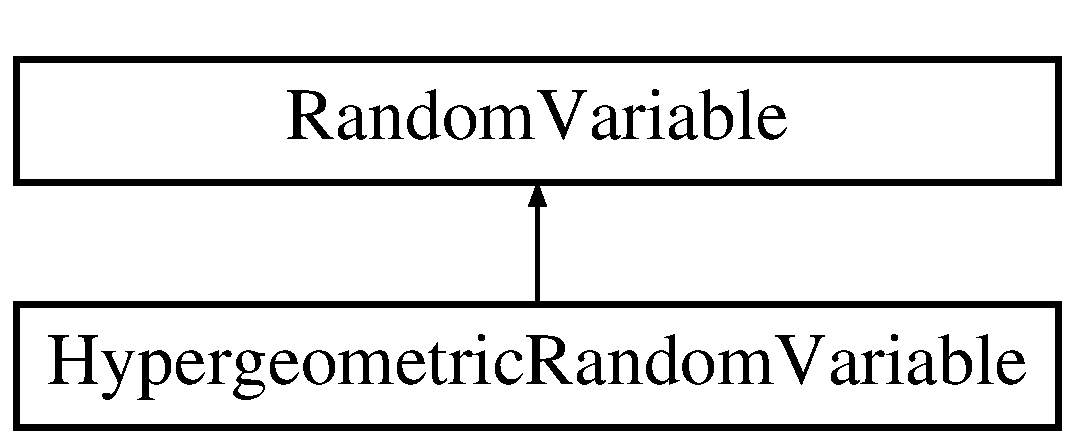
\includegraphics[height=2.000000cm]{classPecos_1_1HypergeometricRandomVariable}
\end{center}
\end{figure}
\subsection*{Public Member Functions}
\begin{DoxyCompactItemize}
\item 
\hyperlink{classPecos_1_1HypergeometricRandomVariable_a134b5b3f9ccb8a93e07c5c62083001bd}{Hypergeometric\+Random\+Variable} ()\label{classPecos_1_1HypergeometricRandomVariable_a134b5b3f9ccb8a93e07c5c62083001bd}

\begin{DoxyCompactList}\small\item\em default constructor \end{DoxyCompactList}\item 
\hyperlink{classPecos_1_1HypergeometricRandomVariable_aa375499baa668f2f762ec824b1d8a978}{Hypergeometric\+Random\+Variable} (unsigned int num\+\_\+total\+\_\+pop, unsigned int num\+\_\+sel\+\_\+pop, unsigned int num\+\_\+fail)\label{classPecos_1_1HypergeometricRandomVariable_aa375499baa668f2f762ec824b1d8a978}

\begin{DoxyCompactList}\small\item\em alternate constructor \end{DoxyCompactList}\item 
\hyperlink{classPecos_1_1HypergeometricRandomVariable_a899daf62a239bccfe0eb02eac9057b8a}{$\sim$\+Hypergeometric\+Random\+Variable} ()\label{classPecos_1_1HypergeometricRandomVariable_a899daf62a239bccfe0eb02eac9057b8a}

\begin{DoxyCompactList}\small\item\em destructor \end{DoxyCompactList}\item 
Real \hyperlink{classPecos_1_1HypergeometricRandomVariable_addd564e7f4f314e12d38df74d845f0d8}{cdf} (Real x) const \label{classPecos_1_1HypergeometricRandomVariable_addd564e7f4f314e12d38df74d845f0d8}

\begin{DoxyCompactList}\small\item\em return the cumulative distribution function value of the random variable at x \end{DoxyCompactList}\item 
Real \hyperlink{classPecos_1_1HypergeometricRandomVariable_a23c3b599e7e4788a9a5e9e93c3dbaf4d}{ccdf} (Real x) const \label{classPecos_1_1HypergeometricRandomVariable_a23c3b599e7e4788a9a5e9e93c3dbaf4d}

\begin{DoxyCompactList}\small\item\em return the complementary cumulative distribution function value of the random variable at x \end{DoxyCompactList}\item 
Real \hyperlink{classPecos_1_1HypergeometricRandomVariable_a918a1aac05ca349ea5313eebcba46c3e}{inverse\+\_\+cdf} (Real p\+\_\+cdf) const \label{classPecos_1_1HypergeometricRandomVariable_a918a1aac05ca349ea5313eebcba46c3e}

\begin{DoxyCompactList}\small\item\em return the x value corresponding to a cumulative probability \end{DoxyCompactList}\item 
Real \hyperlink{classPecos_1_1HypergeometricRandomVariable_afda003a1f59ff6930902cd5c8601f49b}{inverse\+\_\+ccdf} (Real p\+\_\+ccdf) const \label{classPecos_1_1HypergeometricRandomVariable_afda003a1f59ff6930902cd5c8601f49b}

\begin{DoxyCompactList}\small\item\em return the x value corresponding to a complementary cumulative probability \end{DoxyCompactList}\item 
Real \hyperlink{classPecos_1_1HypergeometricRandomVariable_a8ec69265f428e17c1707133cb137a819}{pdf} (Real x) const \label{classPecos_1_1HypergeometricRandomVariable_a8ec69265f428e17c1707133cb137a819}

\begin{DoxyCompactList}\small\item\em return the value of the random variable\textquotesingle{}s probability density function at x \end{DoxyCompactList}\item 
Real \hyperlink{classPecos_1_1HypergeometricRandomVariable_aa891dab1ae9a225f493e3a0e5032b778}{parameter} (short dist\+\_\+param) const \label{classPecos_1_1HypergeometricRandomVariable_aa891dab1ae9a225f493e3a0e5032b778}

\begin{DoxyCompactList}\small\item\em return the value of the named distribution parameter \end{DoxyCompactList}\item 
void \hyperlink{classPecos_1_1HypergeometricRandomVariable_ae8e123224f588aee676d5d56d5ca900d}{parameter} (short dist\+\_\+param, Real val)\label{classPecos_1_1HypergeometricRandomVariable_ae8e123224f588aee676d5d56d5ca900d}

\begin{DoxyCompactList}\small\item\em update the value of the named distribution parameter \end{DoxyCompactList}\item 
Real \hyperlink{classPecos_1_1HypergeometricRandomVariable_a962ffe5a3593be370d5c883365c060f4}{mean} () const \label{classPecos_1_1HypergeometricRandomVariable_a962ffe5a3593be370d5c883365c060f4}

\begin{DoxyCompactList}\small\item\em return the distribution mean \end{DoxyCompactList}\item 
Real \hyperlink{classPecos_1_1HypergeometricRandomVariable_ae1fff19ce29a79d657043a598523635d}{median} () const \label{classPecos_1_1HypergeometricRandomVariable_ae1fff19ce29a79d657043a598523635d}

\begin{DoxyCompactList}\small\item\em return the distribution mode \end{DoxyCompactList}\item 
Real \hyperlink{classPecos_1_1HypergeometricRandomVariable_a72d3d6926edd929cb3f8e12baa655f70}{mode} () const \label{classPecos_1_1HypergeometricRandomVariable_a72d3d6926edd929cb3f8e12baa655f70}

\begin{DoxyCompactList}\small\item\em return the distribution mode \end{DoxyCompactList}\item 
Real \hyperlink{classPecos_1_1HypergeometricRandomVariable_a6a4ed9624d511f8a4e4f509c82cb0706}{standard\+\_\+deviation} () const \label{classPecos_1_1HypergeometricRandomVariable_a6a4ed9624d511f8a4e4f509c82cb0706}

\begin{DoxyCompactList}\small\item\em return the distribution variance \end{DoxyCompactList}\item 
Real \hyperlink{classPecos_1_1HypergeometricRandomVariable_a4b8b05b2a9af92dad9cc304c2925a4eb}{variance} () const \label{classPecos_1_1HypergeometricRandomVariable_a4b8b05b2a9af92dad9cc304c2925a4eb}

\begin{DoxyCompactList}\small\item\em return the distribution variance \end{DoxyCompactList}\item 
Real\+Real\+Pair \hyperlink{classPecos_1_1HypergeometricRandomVariable_a4bdb95a8fa5fffaa0de5102f56963cf2}{bounds} () const \label{classPecos_1_1HypergeometricRandomVariable_a4bdb95a8fa5fffaa0de5102f56963cf2}

\begin{DoxyCompactList}\small\item\em return the distribution lower and upper bounds as a pair \end{DoxyCompactList}\item 
void {\bfseries update} (unsigned int num\+\_\+total\+\_\+pop, unsigned int num\+\_\+sel\+\_\+pop, unsigned int num\+\_\+fail)\label{classPecos_1_1HypergeometricRandomVariable_aac16771ac4604936c4ec99a1d665681b}

\end{DoxyCompactItemize}
\subsection*{Static Public Member Functions}
\begin{DoxyCompactItemize}
\item 
static Real {\bfseries pdf} (Real x, unsigned int num\+\_\+total\+\_\+pop, unsigned int num\+\_\+sel\+\_\+pop, unsigned int num\+\_\+fail)\label{classPecos_1_1HypergeometricRandomVariable_ad536f2435516578fc4c52f0ebb38d118}

\item 
static Real {\bfseries cdf} (Real x, unsigned int num\+\_\+total\+\_\+pop, unsigned int num\+\_\+sel\+\_\+pop, unsigned int num\+\_\+fail)\label{classPecos_1_1HypergeometricRandomVariable_a449e63e2051ca3d9edb98cf6818b11eb}

\item 
static void {\bfseries moments\+\_\+from\+\_\+params} (unsigned int num\+\_\+total\+\_\+pop, unsigned int num\+\_\+sel\+\_\+pop, unsigned int num\+\_\+fail, Real \&\hyperlink{classPecos_1_1HypergeometricRandomVariable_a962ffe5a3593be370d5c883365c060f4}{mean}, Real \&std\+\_\+dev)\label{classPecos_1_1HypergeometricRandomVariable_adcb597703487a69778a15aed04d8ebc0}

\end{DoxyCompactItemize}
\subsection*{Protected Member Functions}
\begin{DoxyCompactItemize}
\item 
void \hyperlink{classPecos_1_1HypergeometricRandomVariable_aaa6750cbee2245416a6eeeac58d4405a}{update\+\_\+boost} ()\label{classPecos_1_1HypergeometricRandomVariable_aaa6750cbee2245416a6eeeac58d4405a}

\begin{DoxyCompactList}\small\item\em create a new hypergeom\+Dist instance \end{DoxyCompactList}\end{DoxyCompactItemize}
\subsection*{Protected Attributes}
\begin{DoxyCompactItemize}
\item 
unsigned int \hyperlink{classPecos_1_1HypergeometricRandomVariable_a248689a7f4ef45f8be7d47d6e3fe142f}{num\+Total\+Pop}\label{classPecos_1_1HypergeometricRandomVariable_a248689a7f4ef45f8be7d47d6e3fe142f}

\begin{DoxyCompactList}\small\item\em N parameter of hypergeometric random variable. \end{DoxyCompactList}\item 
unsigned int \hyperlink{classPecos_1_1HypergeometricRandomVariable_ab382104add8d274e7e7d27561f38a33a}{num\+Select\+Pop}\label{classPecos_1_1HypergeometricRandomVariable_ab382104add8d274e7e7d27561f38a33a}

\begin{DoxyCompactList}\small\item\em n parameter of hypergeometric random variable \end{DoxyCompactList}\item 
unsigned int \hyperlink{classPecos_1_1HypergeometricRandomVariable_a03eaaa9ed47767dd148b221ca4d72b76}{num\+Fail}\label{classPecos_1_1HypergeometricRandomVariable_a03eaaa9ed47767dd148b221ca4d72b76}

\begin{DoxyCompactList}\small\item\em r parameter of hypergeometric random variable \end{DoxyCompactList}\item 
hypergeometric\+\_\+dist $\ast$ \hyperlink{classPecos_1_1HypergeometricRandomVariable_a7a89ee348e50ca9eb7545b5c9fe9f441}{hypergeom\+Dist}\label{classPecos_1_1HypergeometricRandomVariable_a7a89ee348e50ca9eb7545b5c9fe9f441}

\begin{DoxyCompactList}\small\item\em pointer to the Boost hypergeometric\+\_\+distribution instance \end{DoxyCompactList}\end{DoxyCompactItemize}


\subsection{Detailed Description}
Derived random variable class for hypergeometric random variables. 

Manages num\+Total\+Pop, num\+Select\+Pop, and num\+Fail parameters. 

The documentation for this class was generated from the following file\+:\begin{DoxyCompactItemize}
\item 
Hypergeometric\+Random\+Variable.\+hpp\end{DoxyCompactItemize}

\section{Integration\+Driver Class Reference}
\label{classPecos_1_1IntegrationDriver}\index{Integration\+Driver@{Integration\+Driver}}


base class for generating N-\/dimensional grids for numerical evaluation of expectation integrals over independent standard random variables.  


Inheritance diagram for Integration\+Driver\+:\begin{figure}[H]
\begin{center}
\leavevmode
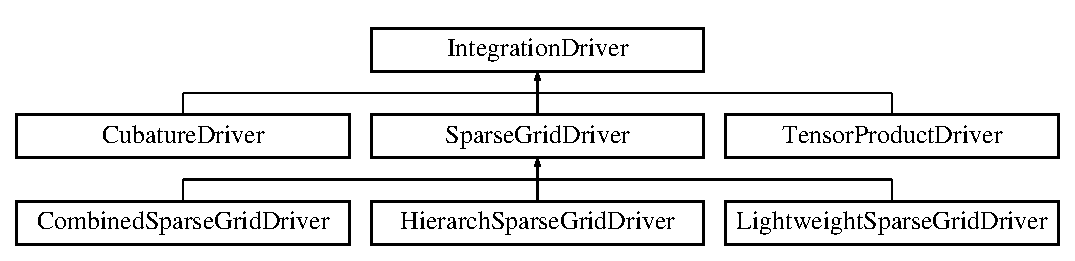
\includegraphics[height=3.000000cm]{classPecos_1_1IntegrationDriver}
\end{center}
\end{figure}
\subsection*{Public Member Functions}
\begin{DoxyCompactItemize}
\item 
\hyperlink{classPecos_1_1IntegrationDriver_af9a391517a476eb80874585a92fa68ba}{Integration\+Driver} ()
\begin{DoxyCompactList}\small\item\em default constructor \end{DoxyCompactList}\item 
\hyperlink{classPecos_1_1IntegrationDriver_a6767d009675093573bb221296e5dbbda}{Integration\+Driver} (short driver\+\_\+type)
\begin{DoxyCompactList}\small\item\em standard constructor for envelope \end{DoxyCompactList}\item 
\hyperlink{classPecos_1_1IntegrationDriver_aa971c023ca4719e4e984744f8aa1cfe4}{Integration\+Driver} (const \hyperlink{classPecos_1_1IntegrationDriver}{Integration\+Driver} \&driver)
\begin{DoxyCompactList}\small\item\em copy constructor \end{DoxyCompactList}\item 
virtual \hyperlink{classPecos_1_1IntegrationDriver_a626671e21974dde95474a2a0f80ffc39}{$\sim$\+Integration\+Driver} ()
\begin{DoxyCompactList}\small\item\em destructor \end{DoxyCompactList}\item 
\hyperlink{classPecos_1_1IntegrationDriver}{Integration\+Driver} \hyperlink{classPecos_1_1IntegrationDriver_a7a2037e44bf9f6373cfd1bd2e80654ae}{operator=} (const \hyperlink{classPecos_1_1IntegrationDriver}{Integration\+Driver} \&driver)
\begin{DoxyCompactList}\small\item\em assignment operator \end{DoxyCompactList}\item 
virtual void \hyperlink{classPecos_1_1IntegrationDriver_a4a1a63a0f30824fcd233da026bdebef6}{initialize\+\_\+grid} (const std\+::vector$<$ \hyperlink{classPecos_1_1BasisPolynomial}{Basis\+Polynomial} $>$ \&poly\+\_\+basis)
\begin{DoxyCompactList}\small\item\em initialize all grid settings (distribution params already set within poly\+\_\+basis) \end{DoxyCompactList}\item 
virtual void \hyperlink{classPecos_1_1IntegrationDriver_a859f844ea03119f1e58183b8bb29f09b}{initialize\+\_\+grid} (const Short\+Array \&u\+\_\+types, const \hyperlink{classPecos_1_1ExpansionConfigOptions}{Expansion\+Config\+Options} \&ec\+\_\+options, const \hyperlink{classPecos_1_1BasisConfigOptions}{Basis\+Config\+Options} \&bc\+\_\+options)
\begin{DoxyCompactList}\small\item\em set int\+\_\+rules and growth\+\_\+rules from u\+\_\+types and mode booleans \end{DoxyCompactList}\item 
virtual void \hyperlink{classPecos_1_1IntegrationDriver_ad6505ab02359090a3dd26f8d3a232575}{initialize\+\_\+grid\+\_\+parameters} (const Short\+Array \&u\+\_\+types, const \hyperlink{classPecos_1_1AleatoryDistParams}{Aleatory\+Dist\+Params} \&adp)\label{classPecos_1_1IntegrationDriver_ad6505ab02359090a3dd26f8d3a232575}

\begin{DoxyCompactList}\small\item\em update polynomial\+Basis with data from \hyperlink{classPecos_1_1AleatoryDistParams}{Aleatory\+Dist\+Params} \end{DoxyCompactList}\item 
virtual void \hyperlink{classPecos_1_1IntegrationDriver_a30b0bccf09758808aeb7e9ca33fae2ff}{compute\+\_\+grid} (Real\+Matrix \&var\+\_\+sets)\label{classPecos_1_1IntegrationDriver_a30b0bccf09758808aeb7e9ca33fae2ff}

\begin{DoxyCompactList}\small\item\em compute scaled variable and weight sets for the T\+PQ grid \end{DoxyCompactList}\item 
virtual int \hyperlink{classPecos_1_1IntegrationDriver_a4b04c73f01f5eb9e6171305141eb1f73}{grid\+\_\+size} ()\label{classPecos_1_1IntegrationDriver_a4b04c73f01f5eb9e6171305141eb1f73}

\begin{DoxyCompactList}\small\item\em compute number of collocation points \end{DoxyCompactList}\item 
virtual void \hyperlink{classPecos_1_1IntegrationDriver_a875c01d83eb38586e43712a94e713312}{reinterpolated\+\_\+tensor\+\_\+grid} (const U\+Short\+Array \&lev\+\_\+index, const Sizet\+List \&reinterp\+\_\+indices)\label{classPecos_1_1IntegrationDriver_a875c01d83eb38586e43712a94e713312}

\begin{DoxyCompactList}\small\item\em computes and stores data for reinterpolation of covariance on a higher-\/order tensor grid \end{DoxyCompactList}\item 
virtual void \hyperlink{classPecos_1_1IntegrationDriver_aeae6e6d94a2e3e77d612eee151c77799}{store\+\_\+grid} (size\+\_\+t index=\+\_\+\+N\+P\+OS)\label{classPecos_1_1IntegrationDriver_aeae6e6d94a2e3e77d612eee151c77799}

\begin{DoxyCompactList}\small\item\em store configuration settings for the current grid before advancing to the next settings within a prescribed grid sequence (default is push\+\_\+back) \end{DoxyCompactList}\item 
virtual void \hyperlink{classPecos_1_1IntegrationDriver_a31ba839ff630bbc25292b448fff38a73}{restore\+\_\+grid} (size\+\_\+t index=\+\_\+\+N\+P\+OS)\label{classPecos_1_1IntegrationDriver_a31ba839ff630bbc25292b448fff38a73}

\begin{DoxyCompactList}\small\item\em restore configuration settings from a previously stored grid \end{DoxyCompactList}\item 
virtual void \hyperlink{classPecos_1_1IntegrationDriver_a93215ecdfbc51b7c45998fa4d65fc7fd}{remove\+\_\+stored\+\_\+grid} (size\+\_\+t index=\+\_\+\+N\+P\+OS)\label{classPecos_1_1IntegrationDriver_a93215ecdfbc51b7c45998fa4d65fc7fd}

\begin{DoxyCompactList}\small\item\em remove configuration settings for a stored grid (default is pop\+\_\+back) \end{DoxyCompactList}\item 
virtual void \hyperlink{classPecos_1_1IntegrationDriver_ae4337960917eda26a5672e5c6afbb62a}{clear\+\_\+stored} ()\label{classPecos_1_1IntegrationDriver_ae4337960917eda26a5672e5c6afbb62a}

\begin{DoxyCompactList}\small\item\em clear stored grid settings following their usage/combination \end{DoxyCompactList}\item 
virtual size\+\_\+t \hyperlink{classPecos_1_1IntegrationDriver_a6edda8aad31eb8a64e180e6a76a6e0e9}{maximal\+\_\+grid} () const \label{classPecos_1_1IntegrationDriver_a6edda8aad31eb8a64e180e6a76a6e0e9}

\begin{DoxyCompactList}\small\item\em return the index of the maximal stored grid state (\+\_\+\+N\+P\+OS if the current unstored grid state) \end{DoxyCompactList}\item 
virtual void \hyperlink{classPecos_1_1IntegrationDriver_ae42d43e21fe55d5b6cca7edf86e54818}{swap\+\_\+grid} (size\+\_\+t index)\label{classPecos_1_1IntegrationDriver_ae42d43e21fe55d5b6cca7edf86e54818}

\begin{DoxyCompactList}\small\item\em swap settings between the current grid and the stored grid identified by index \end{DoxyCompactList}\item 
virtual const Real\+Vector \& \hyperlink{classPecos_1_1IntegrationDriver_ae858d8bd4c244a98b0ff43c979b65e69}{type1\+\_\+weight\+\_\+sets} () const \label{classPecos_1_1IntegrationDriver_ae858d8bd4c244a98b0ff43c979b65e69}

\begin{DoxyCompactList}\small\item\em return type1\+Weight\+Sets from Cubature/\+Tensor\+Product/\+Combined\+Sparse\+Grid or concatenate type1\+Weight\+Sets in Hierarch\+Sparse\+Grid \end{DoxyCompactList}\item 
virtual const Real\+Matrix \& \hyperlink{classPecos_1_1IntegrationDriver_aacf52fa6f04443949a70c62ee3d718f7}{type2\+\_\+weight\+\_\+sets} () const \label{classPecos_1_1IntegrationDriver_aacf52fa6f04443949a70c62ee3d718f7}

\begin{DoxyCompactList}\small\item\em return type2\+Weight\+Sets from Cubature/\+Tensor\+Product/\+Combined\+Sparse\+Grid or concatenate type2\+Weight\+Sets in Hierarch\+Sparse\+Grid \end{DoxyCompactList}\item 
void \hyperlink{classPecos_1_1IntegrationDriver_ad25bbad4ddfa540696bd48d4a81c04dc}{assign\+\_\+rep} (\hyperlink{classPecos_1_1IntegrationDriver}{Integration\+Driver} $\ast$\hyperlink{classPecos_1_1IntegrationDriver_ad9ffab47d51875c80dc41a1ec9980649}{driver\+\_\+rep}, bool ref\+\_\+count\+\_\+incr)\label{classPecos_1_1IntegrationDriver_ad25bbad4ddfa540696bd48d4a81c04dc}

\begin{DoxyCompactList}\small\item\em assign letter or replace existing letter with a new one \end{DoxyCompactList}\item 
void \hyperlink{classPecos_1_1IntegrationDriver_a829957a61b9d2415054771d12a06d660}{compute\+\_\+tensor\+\_\+grid} (const U\+Short\+Array \&quad\+\_\+order, const U\+Short\+Array \&lev\+\_\+index, const Sizet\+List \&subset\+\_\+indices, Real\+Matrix \&variable\+\_\+sets, U\+Short2\+D\+Array \&colloc\+\_\+key)\label{classPecos_1_1IntegrationDriver_a829957a61b9d2415054771d12a06d660}

\begin{DoxyCompactList}\small\item\em compute variable sets for a tensor-\/product grid \end{DoxyCompactList}\item 
void \hyperlink{classPecos_1_1IntegrationDriver_a8c5ab9e65aea318db31dce4410e4b909}{update\+\_\+1d\+\_\+collocation\+\_\+points\+\_\+weights} (const U\+Short\+Array \&quad\+\_\+order, const U\+Short\+Array \&lev\+\_\+index)\label{classPecos_1_1IntegrationDriver_a8c5ab9e65aea318db31dce4410e4b909}

\begin{DoxyCompactList}\small\item\em update colloc\+Pts1D and type\{1,2\}Colloc\+Wts1D \end{DoxyCompactList}\item 
const std\+::vector$<$ \hyperlink{classPecos_1_1BasisPolynomial}{Basis\+Polynomial} $>$ \& \hyperlink{classPecos_1_1IntegrationDriver_a7282b8c27142b1b15cd79922c3f55e19}{polynomial\+\_\+basis} () const \label{classPecos_1_1IntegrationDriver_a7282b8c27142b1b15cd79922c3f55e19}

\begin{DoxyCompactList}\small\item\em return polynomial\+Basis \end{DoxyCompactList}\item 
void \hyperlink{classPecos_1_1IntegrationDriver_ad990c7645a566210244477bec9e46b6d}{mode} (short driver\+\_\+mode)\label{classPecos_1_1IntegrationDriver_ad990c7645a566210244477bec9e46b6d}

\begin{DoxyCompactList}\small\item\em set driver\+Mode \end{DoxyCompactList}\item 
short \hyperlink{classPecos_1_1IntegrationDriver_a1dd1bfd9a642c71eec4df843fd722aad}{mode} () const \label{classPecos_1_1IntegrationDriver_a1dd1bfd9a642c71eec4df843fd722aad}

\begin{DoxyCompactList}\small\item\em get driver\+Mode \end{DoxyCompactList}\item 
const Real3\+D\+Array \& \hyperlink{classPecos_1_1IntegrationDriver_a488137c62d71cae818431be7e1eeab3b}{collocation\+\_\+points\+\_\+1d} () const \label{classPecos_1_1IntegrationDriver_a488137c62d71cae818431be7e1eeab3b}

\begin{DoxyCompactList}\small\item\em return colloc\+Pts1D \end{DoxyCompactList}\item 
const Real3\+D\+Array \& \hyperlink{classPecos_1_1IntegrationDriver_ad6170aa4e92461ebca5e36ad348f82b3}{type1\+\_\+collocation\+\_\+weights\+\_\+1d} () const \label{classPecos_1_1IntegrationDriver_ad6170aa4e92461ebca5e36ad348f82b3}

\begin{DoxyCompactList}\small\item\em return type1\+Colloc\+Wts1D \end{DoxyCompactList}\item 
const Real3\+D\+Array \& \hyperlink{classPecos_1_1IntegrationDriver_a91e8412c2c4ee9a7bdc0f4d67922c03e}{type2\+\_\+collocation\+\_\+weights\+\_\+1d} () const \label{classPecos_1_1IntegrationDriver_a91e8412c2c4ee9a7bdc0f4d67922c03e}

\begin{DoxyCompactList}\small\item\em return type2\+Colloc\+Wts1D \end{DoxyCompactList}\item 
const Short\+Array \& \hyperlink{classPecos_1_1IntegrationDriver_a2b29939dfa7c8ae5fb55e0bdc321a140}{collocation\+\_\+rules} () const \label{classPecos_1_1IntegrationDriver_a2b29939dfa7c8ae5fb55e0bdc321a140}

\begin{DoxyCompactList}\small\item\em return colloc\+Rules \end{DoxyCompactList}\item 
const U\+Short\+Array \& \hyperlink{classPecos_1_1IntegrationDriver_af8a53a60055413e18c885193ada0701e}{reinterpolated\+\_\+level\+\_\+index} () const \label{classPecos_1_1IntegrationDriver_af8a53a60055413e18c885193ada0701e}

\begin{DoxyCompactList}\small\item\em return reinterp\+Level\+Indices\mbox{[}active\+Reinterp\+Index\mbox{]} \end{DoxyCompactList}\item 
const U\+Short\+Array \& \hyperlink{classPecos_1_1IntegrationDriver_a1f1fa0a82db79b4e231011ca3a027837}{reinterpolated\+\_\+quadrature\+\_\+order} () const \label{classPecos_1_1IntegrationDriver_a1f1fa0a82db79b4e231011ca3a027837}

\begin{DoxyCompactList}\small\item\em return reinterp\+Quad\+Orders\mbox{[}active\+Reinterp\+Index\mbox{]} \end{DoxyCompactList}\item 
const Real\+Matrix \& \hyperlink{classPecos_1_1IntegrationDriver_a98b3df639857ab489a9368760c15fe25}{reinterpolated\+\_\+variable\+\_\+sets} () const \label{classPecos_1_1IntegrationDriver_a98b3df639857ab489a9368760c15fe25}

\begin{DoxyCompactList}\small\item\em return reinterp\+Var\+Sets\mbox{[}active\+Reinterp\+Index\mbox{]} \end{DoxyCompactList}\item 
const U\+Short2\+D\+Array \& \hyperlink{classPecos_1_1IntegrationDriver_a51c0d1f979921e35e728aa5cde714d47}{reinterpolated\+\_\+collocation\+\_\+key} () const \label{classPecos_1_1IntegrationDriver_a51c0d1f979921e35e728aa5cde714d47}

\begin{DoxyCompactList}\small\item\em return reinterp\+Colloc\+Keys\mbox{[}active\+Reinterp\+Index\mbox{]} \end{DoxyCompactList}\item 
const U\+Short\+Array \& \hyperlink{classPecos_1_1IntegrationDriver_ae6d9d2cb5478b07205eec17c930f5b87}{genz\+\_\+keister\+\_\+order} () const \label{classPecos_1_1IntegrationDriver_ae6d9d2cb5478b07205eec17c930f5b87}

\begin{DoxyCompactList}\small\item\em return order\+Genz\+Keister \end{DoxyCompactList}\item 
const U\+Short\+Array \& \hyperlink{classPecos_1_1IntegrationDriver_a6eef375289da64304c6118582899f8a4}{genz\+\_\+keister\+\_\+precision} () const \label{classPecos_1_1IntegrationDriver_a6eef375289da64304c6118582899f8a4}

\begin{DoxyCompactList}\small\item\em return prec\+Genz\+Keister \end{DoxyCompactList}\item 
\hyperlink{classPecos_1_1IntegrationDriver}{Integration\+Driver} $\ast$ \hyperlink{classPecos_1_1IntegrationDriver_ad9ffab47d51875c80dc41a1ec9980649}{driver\+\_\+rep} () const \label{classPecos_1_1IntegrationDriver_ad9ffab47d51875c80dc41a1ec9980649}

\begin{DoxyCompactList}\small\item\em returns driver\+Rep for access to derived class member functions that are not mapped to the base level \end{DoxyCompactList}\end{DoxyCompactItemize}
\subsection*{Protected Member Functions}
\begin{DoxyCompactItemize}
\item 
\hyperlink{classPecos_1_1IntegrationDriver_a95ed45db74acb6b02ae3905336f25451}{Integration\+Driver} (\hyperlink{structPecos_1_1BaseConstructor}{Base\+Constructor})
\begin{DoxyCompactList}\small\item\em constructor initializes the base class part of letter classes (\hyperlink{structPecos_1_1BaseConstructor}{Base\+Constructor} overloading avoids infinite recursion in the derived class constructors -\/ Coplien, p. 139) \end{DoxyCompactList}\item 
void \hyperlink{classPecos_1_1IntegrationDriver_aaef7045a54c00867c500d106ab208bed}{compute\+\_\+tensor\+\_\+grid} (const U\+Short\+Array \&quad\+\_\+order, const U\+Short\+Array \&lev\+\_\+index, Real\+Matrix \&variable\+\_\+sets, Real\+Vector \&t1\+\_\+weight\+\_\+sets, Real\+Matrix \&t2\+\_\+weight\+\_\+sets, U\+Short2\+D\+Array \&colloc\+\_\+key)\label{classPecos_1_1IntegrationDriver_aaef7045a54c00867c500d106ab208bed}

\begin{DoxyCompactList}\small\item\em compute variable and weight sets for a tensor-\/product grid \end{DoxyCompactList}\item 
void \hyperlink{classPecos_1_1IntegrationDriver_a7293945cf09aa738794cd989b898162d}{update\+\_\+1d\+\_\+collocation\+\_\+points\+\_\+weights} (const U\+Short\+Array \&quad\+\_\+order, const U\+Short\+Array \&lev\+\_\+index, const Sizet\+List \&subset\+\_\+indices)\label{classPecos_1_1IntegrationDriver_a7293945cf09aa738794cd989b898162d}

\begin{DoxyCompactList}\small\item\em update colloc\+Pts1D and type\{1,2\}Colloc\+Wts1D for subset variables \end{DoxyCompactList}\item 
void \hyperlink{classPecos_1_1IntegrationDriver_a1b43b624d19b7c6370ca6e338399f6ef}{assign\+\_\+1d\+\_\+collocation\+\_\+points\+\_\+weights} (size\+\_\+t i, unsigned short quad\+\_\+order, unsigned short lev\+\_\+index)\label{classPecos_1_1IntegrationDriver_a1b43b624d19b7c6370ca6e338399f6ef}

\begin{DoxyCompactList}\small\item\em update colloc\+Pts1D\mbox{[}lev\+\_\+index\mbox{]}\mbox{[}i\mbox{]} and type\{1,2\}Colloc\+Wts1D\mbox{[}lev\+\_\+index\mbox{]}\mbox{[}i\mbox{]} \end{DoxyCompactList}\end{DoxyCompactItemize}
\subsection*{Protected Attributes}
\begin{DoxyCompactItemize}
\item 
size\+\_\+t \hyperlink{classPecos_1_1IntegrationDriver_ab9ee2ca7227d7347a1ddba107ffb039c}{num\+Vars}\label{classPecos_1_1IntegrationDriver_ab9ee2ca7227d7347a1ddba107ffb039c}

\begin{DoxyCompactList}\small\item\em number of variables in the tensor-\/product grid \end{DoxyCompactList}\item 
short \hyperlink{classPecos_1_1IntegrationDriver_a676e4ebc2df53afb30f4a06155bc7d95}{driver\+Mode}\label{classPecos_1_1IntegrationDriver_a676e4ebc2df53afb30f4a06155bc7d95}

\begin{DoxyCompactList}\small\item\em enumeration value indicating I\+N\+T\+E\+G\+R\+A\+T\+I\+O\+N\+\_\+\+M\+O\+DE or I\+N\+T\+E\+R\+P\+O\+L\+A\+T\+I\+O\+N\+\_\+\+M\+O\+DE \end{DoxyCompactList}\item 
Short\+Array \hyperlink{classPecos_1_1IntegrationDriver_acb586d039200f1fb4d6b83b4f8999231}{colloc\+Rules}\label{classPecos_1_1IntegrationDriver_acb586d039200f1fb4d6b83b4f8999231}

\begin{DoxyCompactList}\small\item\em enumeration codes for integration rule options. Manages internal mode switches for 1D polynomial types\+: e.\+g., G\+A\+U\+S\+S\+\_\+\+L\+E\+G\+E\+N\+D\+RE or G\+A\+U\+S\+S\+\_\+\+P\+A\+T\+T\+E\+R\+S\+ON for Legendre, C\+L\+E\+N\+S\+H\+A\+W\+\_\+\+C\+U\+R\+T\+IS or F\+E\+J\+E\+R2 for Chebyshev, G\+A\+U\+S\+S\+\_\+\+H\+E\+R\+M\+I\+TE or G\+E\+N\+Z\+\_\+\+K\+E\+I\+S\+T\+ER for Hermite. \end{DoxyCompactList}\item 
std\+::vector$<$ \hyperlink{classPecos_1_1BasisPolynomial}{Basis\+Polynomial} $>$ \hyperlink{classPecos_1_1IntegrationDriver_a9b1c6d91c0a7c0dcf1c392e5f2481eec}{polynomial\+Basis}\label{classPecos_1_1IntegrationDriver_a9b1c6d91c0a7c0dcf1c392e5f2481eec}

\begin{DoxyCompactList}\small\item\em array of one-\/dimensional orthogonal polynomials used in computing Gaussian quadrature points and weights \end{DoxyCompactList}\item 
Real3\+D\+Array \hyperlink{classPecos_1_1IntegrationDriver_a245992931d5285b87bec708f153a5c70}{colloc\+Pts1D}\label{classPecos_1_1IntegrationDriver_a245992931d5285b87bec708f153a5c70}

\begin{DoxyCompactList}\small\item\em num\+\_\+levels\+\_\+per\+\_\+var x num\+Vars sets of 1D collocation points \end{DoxyCompactList}\item 
Real3\+D\+Array \hyperlink{classPecos_1_1IntegrationDriver_a5af9b398ecf07f41783595ec45b6eafe}{type1\+Colloc\+Wts1D}\label{classPecos_1_1IntegrationDriver_a5af9b398ecf07f41783595ec45b6eafe}

\begin{DoxyCompactList}\small\item\em num\+\_\+levels\+\_\+per\+\_\+var x num\+Vars sets of 1D type1 collocation weights \end{DoxyCompactList}\item 
Real3\+D\+Array \hyperlink{classPecos_1_1IntegrationDriver_aa9a7062cd531acf0f989d6f500724eff}{type2\+Colloc\+Wts1D}\label{classPecos_1_1IntegrationDriver_aa9a7062cd531acf0f989d6f500724eff}

\begin{DoxyCompactList}\small\item\em num\+\_\+levels\+\_\+per\+\_\+var x num\+Vars sets of 1D type2 collocation weights \end{DoxyCompactList}\item 
bool \hyperlink{classPecos_1_1IntegrationDriver_a637037ea4cf412ec8aa2c932c39e8043}{compute\+Type2\+Weights}\label{classPecos_1_1IntegrationDriver_a637037ea4cf412ec8aa2c932c39e8043}

\begin{DoxyCompactList}\small\item\em flag indicating usage of compute1\+D\+Type2\+Weights to define type2\+Weight\+Sets \end{DoxyCompactList}\item 
U\+Short2\+D\+Array \hyperlink{classPecos_1_1IntegrationDriver_a57eaeff5743cf77e1518a2125fa00a72}{reinterp\+Level\+Indices}\label{classPecos_1_1IntegrationDriver_a57eaeff5743cf77e1518a2125fa00a72}

\begin{DoxyCompactList}\small\item\em bookkeeping for reinterpolation of covariance\+: stored level indices \end{DoxyCompactList}\item 
U\+Short2\+D\+Array \hyperlink{classPecos_1_1IntegrationDriver_a991cf5ee032abea7de271eaeb1171e83}{reinterp\+Quad\+Orders}\label{classPecos_1_1IntegrationDriver_a991cf5ee032abea7de271eaeb1171e83}

\begin{DoxyCompactList}\small\item\em bookkeeping for reinterpolation of covariance\+: stored quadrature orders \end{DoxyCompactList}\item 
Real\+Matrix\+Array \hyperlink{classPecos_1_1IntegrationDriver_a836568943c74b58be86137bc53c2dd9d}{reinterp\+Var\+Sets}\label{classPecos_1_1IntegrationDriver_a836568943c74b58be86137bc53c2dd9d}

\begin{DoxyCompactList}\small\item\em bookkeeping for reinterpolation of covariance\+: stored variable sets \end{DoxyCompactList}\item 
U\+Short3\+D\+Array \hyperlink{classPecos_1_1IntegrationDriver_a12f3bb281f37a78329402207b4080931}{reinterp\+Colloc\+Keys}\label{classPecos_1_1IntegrationDriver_a12f3bb281f37a78329402207b4080931}

\begin{DoxyCompactList}\small\item\em bookkeeping for reinterpolation of covariance\+: stored collocation keys \end{DoxyCompactList}\item 
std\+::map$<$ U\+Short\+Array, size\+\_\+t $>$ \hyperlink{classPecos_1_1IntegrationDriver_aa62d46c9b84703ed6f990477167e3899}{reinterp\+Map}\label{classPecos_1_1IntegrationDriver_aa62d46c9b84703ed6f990477167e3899}

\begin{DoxyCompactList}\small\item\em tracks existing reinterpolation grids to avoid unnecessary recomputation \end{DoxyCompactList}\item 
size\+\_\+t \hyperlink{classPecos_1_1IntegrationDriver_a1c170aca651f517a8eacff61aa355559}{active\+Reinterp\+Index}\label{classPecos_1_1IntegrationDriver_a1c170aca651f517a8eacff61aa355559}

\begin{DoxyCompactList}\small\item\em bookkeeping for reinterpolation of covariance\+: active index into arrays \end{DoxyCompactList}\end{DoxyCompactItemize}
\subsection*{Static Protected Attributes}
\begin{DoxyCompactItemize}
\item 
static U\+Short\+Array \hyperlink{classPecos_1_1IntegrationDriver_aaa634e4b0fa4d99e12ffd1f18def2382}{order\+Genz\+Keister}\label{classPecos_1_1IntegrationDriver_aaa634e4b0fa4d99e12ffd1f18def2382}

\begin{DoxyCompactList}\small\item\em lookup for set of 1-\/D Genz-\/\+Keister quadrature orders \end{DoxyCompactList}\item 
static U\+Short\+Array \hyperlink{classPecos_1_1IntegrationDriver_afa718e981f5bfc14c6c78ac59e46994e}{prec\+Genz\+Keister}\label{classPecos_1_1IntegrationDriver_afa718e981f5bfc14c6c78ac59e46994e}

\begin{DoxyCompactList}\small\item\em lookup for set of 1-\/D Genz-\/\+Keister integrand precisions \end{DoxyCompactList}\end{DoxyCompactItemize}
\subsection*{Private Member Functions}
\begin{DoxyCompactItemize}
\item 
\hyperlink{classPecos_1_1IntegrationDriver}{Integration\+Driver} $\ast$ \hyperlink{classPecos_1_1IntegrationDriver_a2c88277b463a123722a4f252fdb16bba}{get\+\_\+driver} (short driver\+\_\+type)
\begin{DoxyCompactList}\small\item\em Used only by the standard envelope constructor to initialize driver\+Rep to the appropriate derived type. \end{DoxyCompactList}\end{DoxyCompactItemize}
\subsection*{Private Attributes}
\begin{DoxyCompactItemize}
\item 
\hyperlink{classPecos_1_1IntegrationDriver}{Integration\+Driver} $\ast$ \hyperlink{classPecos_1_1IntegrationDriver_af5db1260af15e88b5451fb5c39c66161}{driver\+Rep}\label{classPecos_1_1IntegrationDriver_af5db1260af15e88b5451fb5c39c66161}

\begin{DoxyCompactList}\small\item\em pointer to the letter (initialized only for the envelope) \end{DoxyCompactList}\item 
int \hyperlink{classPecos_1_1IntegrationDriver_afff0b6144883d3ca09a8d0d3f4776b0f}{reference\+Count}\label{classPecos_1_1IntegrationDriver_afff0b6144883d3ca09a8d0d3f4776b0f}

\begin{DoxyCompactList}\small\item\em number of objects sharing driver\+Rep \end{DoxyCompactList}\end{DoxyCompactItemize}


\subsection{Detailed Description}
base class for generating N-\/dimensional grids for numerical evaluation of expectation integrals over independent standard random variables. 

This class enables Dakota\+::\+NonD\{Quadrature,Cubature,Sparse\+Grid\}. 

\subsection{Constructor \& Destructor Documentation}
\index{Pecos\+::\+Integration\+Driver@{Pecos\+::\+Integration\+Driver}!Integration\+Driver@{Integration\+Driver}}
\index{Integration\+Driver@{Integration\+Driver}!Pecos\+::\+Integration\+Driver@{Pecos\+::\+Integration\+Driver}}
\subsubsection[{\texorpdfstring{Integration\+Driver()}{IntegrationDriver()}}]{\setlength{\rightskip}{0pt plus 5cm}{\bf Integration\+Driver} (
\begin{DoxyParamCaption}
{}
\end{DoxyParamCaption}
)}\label{classPecos_1_1IntegrationDriver_af9a391517a476eb80874585a92fa68ba}


default constructor 

The default constructor\+: driver\+Rep is N\+U\+LL in this case. This makes it necessary to check for N\+U\+LL in the copy constructor, assignment operator, and destructor. \index{Pecos\+::\+Integration\+Driver@{Pecos\+::\+Integration\+Driver}!Integration\+Driver@{Integration\+Driver}}
\index{Integration\+Driver@{Integration\+Driver}!Pecos\+::\+Integration\+Driver@{Pecos\+::\+Integration\+Driver}}
\subsubsection[{\texorpdfstring{Integration\+Driver(short driver\+\_\+type)}{IntegrationDriver(short driver_type)}}]{\setlength{\rightskip}{0pt plus 5cm}{\bf Integration\+Driver} (
\begin{DoxyParamCaption}
\item[{short}]{driver\+\_\+type}
\end{DoxyParamCaption}
)}\label{classPecos_1_1IntegrationDriver_a6767d009675093573bb221296e5dbbda}


standard constructor for envelope 

Envelope constructor only needs to extract enough data to properly execute get\+\_\+driver, since \hyperlink{classPecos_1_1IntegrationDriver_a95ed45db74acb6b02ae3905336f25451}{Integration\+Driver(\+Base\+Constructor)} builds the actual base class data for the derived basis functions. 

References Integration\+Driver\+::driver\+Rep, and Integration\+Driver\+::get\+\_\+driver().

\index{Pecos\+::\+Integration\+Driver@{Pecos\+::\+Integration\+Driver}!Integration\+Driver@{Integration\+Driver}}
\index{Integration\+Driver@{Integration\+Driver}!Pecos\+::\+Integration\+Driver@{Pecos\+::\+Integration\+Driver}}
\subsubsection[{\texorpdfstring{Integration\+Driver(const Integration\+Driver \&driver)}{IntegrationDriver(const IntegrationDriver &driver)}}]{\setlength{\rightskip}{0pt plus 5cm}{\bf Integration\+Driver} (
\begin{DoxyParamCaption}
\item[{const {\bf Integration\+Driver} \&}]{driver}
\end{DoxyParamCaption}
)}\label{classPecos_1_1IntegrationDriver_aa971c023ca4719e4e984744f8aa1cfe4}


copy constructor 

Copy constructor manages sharing of driver\+Rep and incrementing of reference\+Count. 

References Integration\+Driver\+::driver\+Rep, and Integration\+Driver\+::reference\+Count.

\index{Pecos\+::\+Integration\+Driver@{Pecos\+::\+Integration\+Driver}!````~Integration\+Driver@{$\sim$\+Integration\+Driver}}
\index{````~Integration\+Driver@{$\sim$\+Integration\+Driver}!Pecos\+::\+Integration\+Driver@{Pecos\+::\+Integration\+Driver}}
\subsubsection[{\texorpdfstring{$\sim$\+Integration\+Driver()}{~IntegrationDriver()}}]{\setlength{\rightskip}{0pt plus 5cm}$\sim${\bf Integration\+Driver} (
\begin{DoxyParamCaption}
{}
\end{DoxyParamCaption}
)\hspace{0.3cm}{\ttfamily [virtual]}}\label{classPecos_1_1IntegrationDriver_a626671e21974dde95474a2a0f80ffc39}


destructor 

Destructor decrements reference\+Count and only deletes driver\+Rep when reference\+Count reaches zero. 

References Integration\+Driver\+::assign\+\_\+rep(), Integration\+Driver\+::driver\+Rep, and Integration\+Driver\+::reference\+Count.

\index{Pecos\+::\+Integration\+Driver@{Pecos\+::\+Integration\+Driver}!Integration\+Driver@{Integration\+Driver}}
\index{Integration\+Driver@{Integration\+Driver}!Pecos\+::\+Integration\+Driver@{Pecos\+::\+Integration\+Driver}}
\subsubsection[{\texorpdfstring{Integration\+Driver(\+Base\+Constructor)}{IntegrationDriver(BaseConstructor)}}]{\setlength{\rightskip}{0pt plus 5cm}{\bf Integration\+Driver} (
\begin{DoxyParamCaption}
\item[{{\bf Base\+Constructor}}]{}
\end{DoxyParamCaption}
)\hspace{0.3cm}{\ttfamily [protected]}}\label{classPecos_1_1IntegrationDriver_a95ed45db74acb6b02ae3905336f25451}


constructor initializes the base class part of letter classes (\hyperlink{structPecos_1_1BaseConstructor}{Base\+Constructor} overloading avoids infinite recursion in the derived class constructors -\/ Coplien, p. 139) 

This constructor is the one which must build the base class data for all derived classes. \hyperlink{classPecos_1_1IntegrationDriver_a2c88277b463a123722a4f252fdb16bba}{get\+\_\+driver()} instantiates a derived class letter and the derived constructor selects this base class constructor in its initialization list (to avoid recursion in the base class constructor calling \hyperlink{classPecos_1_1IntegrationDriver_a2c88277b463a123722a4f252fdb16bba}{get\+\_\+driver()} again). Since the letter IS the representation, its rep pointer is set to N\+U\+LL (an uninitialized pointer causes problems in $\sim$\+Integration\+Driver). 

References Integration\+Driver\+::order\+Genz\+Keister, and Integration\+Driver\+::prec\+Genz\+Keister.



\subsection{Member Function Documentation}
\index{Pecos\+::\+Integration\+Driver@{Pecos\+::\+Integration\+Driver}!operator=@{operator=}}
\index{operator=@{operator=}!Pecos\+::\+Integration\+Driver@{Pecos\+::\+Integration\+Driver}}
\subsubsection[{\texorpdfstring{operator=(const Integration\+Driver \&driver)}{operator=(const IntegrationDriver &driver)}}]{\setlength{\rightskip}{0pt plus 5cm}{\bf Integration\+Driver} operator= (
\begin{DoxyParamCaption}
\item[{const {\bf Integration\+Driver} \&}]{driver}
\end{DoxyParamCaption}
)}\label{classPecos_1_1IntegrationDriver_a7a2037e44bf9f6373cfd1bd2e80654ae}


assignment operator 

Assignment operator decrements reference\+Count for old driver\+Rep, assigns new driver\+Rep, and increments reference\+Count for new driver\+Rep. 

References Integration\+Driver\+::driver\+Rep, and Integration\+Driver\+::reference\+Count.

\index{Pecos\+::\+Integration\+Driver@{Pecos\+::\+Integration\+Driver}!initialize\+\_\+grid@{initialize\+\_\+grid}}
\index{initialize\+\_\+grid@{initialize\+\_\+grid}!Pecos\+::\+Integration\+Driver@{Pecos\+::\+Integration\+Driver}}
\subsubsection[{\texorpdfstring{initialize\+\_\+grid(const std\+::vector$<$ Basis\+Polynomial $>$ \&poly\+\_\+basis)}{initialize_grid(const std::vector< BasisPolynomial > &poly_basis)}}]{\setlength{\rightskip}{0pt plus 5cm}void initialize\+\_\+grid (
\begin{DoxyParamCaption}
\item[{const std\+::vector$<$ {\bf Basis\+Polynomial} $>$ \&}]{poly\+\_\+basis}
\end{DoxyParamCaption}
)\hspace{0.3cm}{\ttfamily [virtual]}}\label{classPecos_1_1IntegrationDriver_a4a1a63a0f30824fcd233da026bdebef6}


initialize all grid settings (distribution params already set within poly\+\_\+basis) 

protected function called only from derived class letters. 

Reimplemented in \hyperlink{classPecos_1_1TensorProductDriver_a4a1a63a0f30824fcd233da026bdebef6}{Tensor\+Product\+Driver}, \hyperlink{classPecos_1_1CombinedSparseGridDriver_a4a1a63a0f30824fcd233da026bdebef6}{Combined\+Sparse\+Grid\+Driver}, and \hyperlink{classPecos_1_1CubatureDriver_a4a1a63a0f30824fcd233da026bdebef6}{Cubature\+Driver}.



References Integration\+Driver\+::colloc\+Rules, Integration\+Driver\+::compute\+Type2\+Weights, Integration\+Driver\+::driver\+Rep, Integration\+Driver\+::initialize\+\_\+grid(), Integration\+Driver\+::num\+Vars, and Integration\+Driver\+::polynomial\+Basis.



Referenced by Shared\+Nodal\+Interp\+Poly\+Approx\+Data\+::allocate\+\_\+data(), Integration\+Driver\+::initialize\+\_\+grid(), Combined\+Sparse\+Grid\+Driver\+::initialize\+\_\+grid(), Sparse\+Grid\+Driver\+::initialize\+\_\+grid(), Tensor\+Product\+Driver\+::initialize\+\_\+grid(), and Integration\+Driver\+::type2\+\_\+weight\+\_\+sets().

\index{Pecos\+::\+Integration\+Driver@{Pecos\+::\+Integration\+Driver}!initialize\+\_\+grid@{initialize\+\_\+grid}}
\index{initialize\+\_\+grid@{initialize\+\_\+grid}!Pecos\+::\+Integration\+Driver@{Pecos\+::\+Integration\+Driver}}
\subsubsection[{\texorpdfstring{initialize\+\_\+grid(const Short\+Array \&u\+\_\+types, const Expansion\+Config\+Options \&ec\+\_\+options, const Basis\+Config\+Options \&bc\+\_\+options)}{initialize_grid(const ShortArray &u_types, const ExpansionConfigOptions &ec_options, const BasisConfigOptions &bc_options)}}]{\setlength{\rightskip}{0pt plus 5cm}void initialize\+\_\+grid (
\begin{DoxyParamCaption}
\item[{const Short\+Array \&}]{u\+\_\+types, }
\item[{const {\bf Expansion\+Config\+Options} \&}]{ec\+\_\+options, }
\item[{const {\bf Basis\+Config\+Options} \&}]{bc\+\_\+options}
\end{DoxyParamCaption}
)\hspace{0.3cm}{\ttfamily [virtual]}}\label{classPecos_1_1IntegrationDriver_a859f844ea03119f1e58183b8bb29f09b}


set int\+\_\+rules and growth\+\_\+rules from u\+\_\+types and mode booleans 

protected function called only from derived class letters. 

Reimplemented in \hyperlink{classPecos_1_1TensorProductDriver_a859f844ea03119f1e58183b8bb29f09b}{Tensor\+Product\+Driver}.



References Integration\+Driver\+::colloc\+Rules, Integration\+Driver\+::compute\+Type2\+Weights, Integration\+Driver\+::driver\+Mode, Expansion\+Config\+Options\+::exp\+Basis\+Type, Shared\+Interp\+Poly\+Approx\+Data\+::initialize\+\_\+driver\+\_\+types\+\_\+rules(), Integration\+Driver\+::initialize\+\_\+grid(), Shared\+Poly\+Approx\+Data\+::initialize\+\_\+orthogonal\+\_\+basis\+\_\+types\+\_\+rules(), Shared\+Poly\+Approx\+Data\+::initialize\+\_\+polynomial\+\_\+basis(), Integration\+Driver\+::num\+Vars, and Integration\+Driver\+::polynomial\+Basis.

\index{Pecos\+::\+Integration\+Driver@{Pecos\+::\+Integration\+Driver}!get\+\_\+driver@{get\+\_\+driver}}
\index{get\+\_\+driver@{get\+\_\+driver}!Pecos\+::\+Integration\+Driver@{Pecos\+::\+Integration\+Driver}}
\subsubsection[{\texorpdfstring{get\+\_\+driver(short driver\+\_\+type)}{get_driver(short driver_type)}}]{\setlength{\rightskip}{0pt plus 5cm}{\bf Integration\+Driver} $\ast$ get\+\_\+driver (
\begin{DoxyParamCaption}
\item[{short}]{driver\+\_\+type}
\end{DoxyParamCaption}
)\hspace{0.3cm}{\ttfamily [private]}}\label{classPecos_1_1IntegrationDriver_a2c88277b463a123722a4f252fdb16bba}


Used only by the standard envelope constructor to initialize driver\+Rep to the appropriate derived type. 

Used only by the envelope constructor to initialize driver\+Rep to the appropriate derived type. 

Referenced by Integration\+Driver\+::\+Integration\+Driver().



The documentation for this class was generated from the following files\+:\begin{DoxyCompactItemize}
\item 
Integration\+Driver.\+hpp\item 
Integration\+Driver.\+cpp\end{DoxyCompactItemize}

\section{Interpolation\+Polynomial Class Reference}
\label{classPecos_1_1InterpolationPolynomial}\index{Interpolation\+Polynomial@{Interpolation\+Polynomial}}


Derived basis polynomial class for 1-\/D Lagrange interpolation polynomials.  


Inheritance diagram for Interpolation\+Polynomial\+:\begin{figure}[H]
\begin{center}
\leavevmode
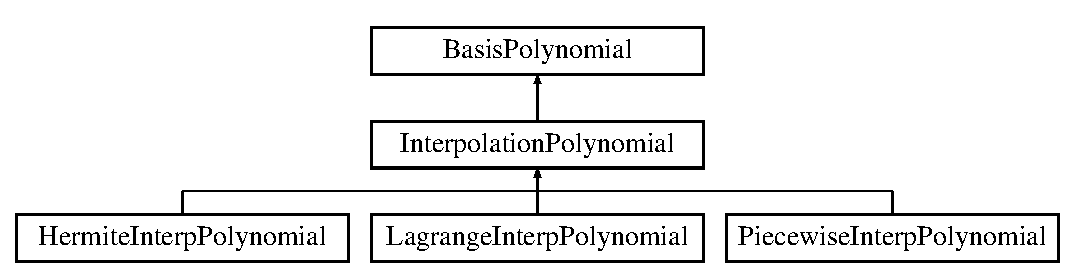
\includegraphics[height=3.000000cm]{classPecos_1_1InterpolationPolynomial}
\end{center}
\end{figure}
\subsection*{Public Member Functions}
\begin{DoxyCompactItemize}
\item 
\hyperlink{classPecos_1_1InterpolationPolynomial_a600a8ab653342299615a8c494aa33a5c}{Interpolation\+Polynomial} ()\label{classPecos_1_1InterpolationPolynomial_a600a8ab653342299615a8c494aa33a5c}

\begin{DoxyCompactList}\small\item\em default constructor \end{DoxyCompactList}\item 
\hyperlink{classPecos_1_1InterpolationPolynomial_a032b69c7d11f948db8cdef4e44d81f25}{Interpolation\+Polynomial} (const Real\+Array \&interp\+\_\+pts)\label{classPecos_1_1InterpolationPolynomial_a032b69c7d11f948db8cdef4e44d81f25}

\begin{DoxyCompactList}\small\item\em standard constructor \end{DoxyCompactList}\item 
virtual \hyperlink{classPecos_1_1InterpolationPolynomial_a3fc5373ce7b55a154e2b21ea7a75098b}{$\sim$\+Interpolation\+Polynomial} ()\label{classPecos_1_1InterpolationPolynomial_a3fc5373ce7b55a154e2b21ea7a75098b}

\begin{DoxyCompactList}\small\item\em destructor \end{DoxyCompactList}\item 
virtual void \hyperlink{classPecos_1_1InterpolationPolynomial_a9a5fd3dc945d15c8423dc66dcd137b4f}{precompute\+\_\+data} ()\label{classPecos_1_1InterpolationPolynomial_a9a5fd3dc945d15c8423dc66dcd137b4f}

\begin{DoxyCompactList}\small\item\em precompute data that is reused repeatedly within interpolation \end{DoxyCompactList}\item 
size\+\_\+t \hyperlink{classPecos_1_1InterpolationPolynomial_a3122d8fb10bc54de12fde87cffdf8fee}{interpolation\+\_\+size} () const \label{classPecos_1_1InterpolationPolynomial_a3122d8fb10bc54de12fde87cffdf8fee}

\begin{DoxyCompactList}\small\item\em get size of interp\+Pts \end{DoxyCompactList}\item 
void \hyperlink{classPecos_1_1InterpolationPolynomial_a6babe691e74f48a1b3597132cc739223}{interpolation\+\_\+points} (const Real\+Array \&interp\+\_\+pts)\label{classPecos_1_1InterpolationPolynomial_a6babe691e74f48a1b3597132cc739223}

\begin{DoxyCompactList}\small\item\em set interp\+Pts \end{DoxyCompactList}\item 
const Real\+Array \& \hyperlink{classPecos_1_1InterpolationPolynomial_af8e63614c42281644c4c0e099fb3e1f8}{interpolation\+\_\+points} () const \label{classPecos_1_1InterpolationPolynomial_af8e63614c42281644c4c0e099fb3e1f8}

\begin{DoxyCompactList}\small\item\em get interp\+Pts \end{DoxyCompactList}\end{DoxyCompactItemize}
\subsection*{Protected Attributes}
\begin{DoxyCompactItemize}
\item 
Real\+Array \hyperlink{classPecos_1_1InterpolationPolynomial_ae944308ccb32a77df689397d462470b4}{interp\+Pts}\label{classPecos_1_1InterpolationPolynomial_ae944308ccb32a77df689397d462470b4}

\begin{DoxyCompactList}\small\item\em set of 1-\/D interpolation points\+: the i\+\_\+th interpolation polynomial evaluated at the j\+\_\+th interpolation point produces Kronecker delta\+\_\+ij \end{DoxyCompactList}\end{DoxyCompactItemize}
\subsection*{Additional Inherited Members}


\subsection{Detailed Description}
Derived basis polynomial class for 1-\/D Lagrange interpolation polynomials. 

The \hyperlink{classPecos_1_1InterpolationPolynomial}{Interpolation\+Polynomial} class evaluates a univariate interpolation polynomial. It enables multidimensional interpolants within \hyperlink{classPecos_1_1InterpPolyApproximation}{Interp\+Poly\+Approximation}. 

The documentation for this class was generated from the following files\+:\begin{DoxyCompactItemize}
\item 
Interpolation\+Polynomial.\+hpp\item 
Interpolation\+Polynomial.\+cpp\end{DoxyCompactItemize}

\section{Interp\+Poly\+Approximation Class Reference}
\label{classPecos_1_1InterpPolyApproximation}\index{Interp\+Poly\+Approximation@{Interp\+Poly\+Approximation}}


Derived approximation class for interpolation polynomials (global approximation).  


Inheritance diagram for Interp\+Poly\+Approximation\+:\begin{figure}[H]
\begin{center}
\leavevmode
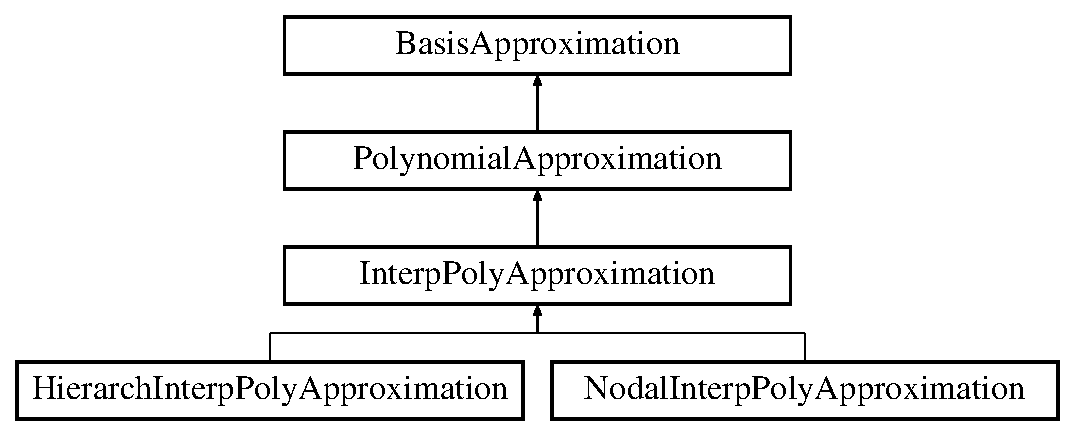
\includegraphics[height=4.000000cm]{classPecos_1_1InterpPolyApproximation}
\end{center}
\end{figure}
\subsection*{Public Member Functions}
\begin{DoxyCompactItemize}
\item 
\hyperlink{classPecos_1_1InterpPolyApproximation_af71906e1c253c3f28a63e602882ab16f}{Interp\+Poly\+Approximation} (const \hyperlink{classPecos_1_1SharedBasisApproxData}{Shared\+Basis\+Approx\+Data} \&shared\+\_\+data)\label{classPecos_1_1InterpPolyApproximation_af71906e1c253c3f28a63e602882ab16f}

\begin{DoxyCompactList}\small\item\em default constructor \end{DoxyCompactList}\item 
\hyperlink{classPecos_1_1InterpPolyApproximation_ab1015d603f22b30086ed9e2a9ef7c4c5}{$\sim$\+Interp\+Poly\+Approximation} ()\label{classPecos_1_1InterpPolyApproximation_ab1015d603f22b30086ed9e2a9ef7c4c5}

\begin{DoxyCompactList}\small\item\em destructor \end{DoxyCompactList}\end{DoxyCompactItemize}
\subsection*{Protected Member Functions}
\begin{DoxyCompactItemize}
\item 
int \hyperlink{classPecos_1_1InterpPolyApproximation_ac789358ee49633613d6c97593be06f9d}{min\+\_\+coefficients} () const \label{classPecos_1_1InterpPolyApproximation_ac789358ee49633613d6c97593be06f9d}

\begin{DoxyCompactList}\small\item\em return the minimum number of samples (unknowns) required to build the derived class approximation type in num\+Vars dimensions \end{DoxyCompactList}\item 
void \hyperlink{classPecos_1_1InterpPolyApproximation_a37ef37829b412fefa40d53b395846781}{allocate\+\_\+arrays} ()\label{classPecos_1_1InterpPolyApproximation_a37ef37829b412fefa40d53b395846781}

\begin{DoxyCompactList}\small\item\em size derived class data attributes \end{DoxyCompactList}\item 
void \hyperlink{classPecos_1_1InterpPolyApproximation_abec3f45a112004b53f83b3a03e0d06db}{compute\+\_\+component\+\_\+sobol} ()\label{classPecos_1_1InterpPolyApproximation_abec3f45a112004b53f83b3a03e0d06db}

\begin{DoxyCompactList}\small\item\em computes component (main and interaction) Sobol\textquotesingle{} indices \end{DoxyCompactList}\item 
void \hyperlink{classPecos_1_1InterpPolyApproximation_ada0deadfa2c3202ed4e58d066ee079f2}{compute\+\_\+total\+\_\+sobol} ()\label{classPecos_1_1InterpPolyApproximation_ada0deadfa2c3202ed4e58d066ee079f2}

\begin{DoxyCompactList}\small\item\em computes total Sobol\textquotesingle{} indices \end{DoxyCompactList}\item 
void \hyperlink{classPecos_1_1InterpPolyApproximation_a5926c67431b0fc223fcfa6c11cb9de14}{compute\+\_\+moments} (bool full\+\_\+stats=true)\label{classPecos_1_1InterpPolyApproximation_a5926c67431b0fc223fcfa6c11cb9de14}

\begin{DoxyCompactList}\small\item\em compute numerical moments to order 4 \end{DoxyCompactList}\item 
void \hyperlink{classPecos_1_1InterpPolyApproximation_a2a6098ab4416bdcfdeadea5d46aa5f52}{compute\+\_\+moments} (const Real\+Vector \&x, bool full\+\_\+stats=true)\label{classPecos_1_1InterpPolyApproximation_a2a6098ab4416bdcfdeadea5d46aa5f52}

\begin{DoxyCompactList}\small\item\em compute numerical moments in all-\/variables mode to order 2 \end{DoxyCompactList}\item 
virtual void \hyperlink{classPecos_1_1InterpPolyApproximation_a49382d77eadd7740d024d1d09d42981a}{integrate\+\_\+response\+\_\+moments} (size\+\_\+t num\+\_\+moments)=0\label{classPecos_1_1InterpPolyApproximation_a49382d77eadd7740d024d1d09d42981a}

\begin{DoxyCompactList}\small\item\em compute moments of response using numerical integration \end{DoxyCompactList}\item 
virtual void \hyperlink{classPecos_1_1InterpPolyApproximation_ab67f32d563b7502bdb0c09e076beaa28}{integrate\+\_\+expansion\+\_\+moments} (size\+\_\+t num\+\_\+moments)=0\label{classPecos_1_1InterpPolyApproximation_ab67f32d563b7502bdb0c09e076beaa28}

\begin{DoxyCompactList}\small\item\em compute moments of expansion using numerical integration \end{DoxyCompactList}\item 
virtual void {\bfseries compute\+\_\+total\+\_\+sobol\+\_\+indices} ()=0\label{classPecos_1_1InterpPolyApproximation_a1c4749d8c520c4fefd4f8bb99af67b65}

\item 
virtual void \hyperlink{classPecos_1_1InterpPolyApproximation_a6eb2548a8c786f48478fabb6377be779}{compute\+\_\+partial\+\_\+variance} (const Bit\+Array \&set\+\_\+value)
\item 
void \hyperlink{classPecos_1_1InterpPolyApproximation_a62194c257129acedb670750a372adb1d}{test\+\_\+interpolation} ()\label{classPecos_1_1InterpPolyApproximation_a62194c257129acedb670750a372adb1d}

\begin{DoxyCompactList}\small\item\em test accuracy of the interpolants \end{DoxyCompactList}\end{DoxyCompactItemize}
\subsection*{Protected Attributes}
\begin{DoxyCompactItemize}
\item 
Real\+Vector \hyperlink{classPecos_1_1InterpPolyApproximation_a4699779299311e1ed28f77eb9ac6d768}{partial\+Variance}\label{classPecos_1_1InterpPolyApproximation_a4699779299311e1ed28f77eb9ac6d768}

\begin{DoxyCompactList}\small\item\em the partial\+Variances of subset functions f\+\_\+alpha \end{DoxyCompactList}\end{DoxyCompactItemize}
\subsection*{Private Member Functions}
\begin{DoxyCompactItemize}
\item 
void \hyperlink{classPecos_1_1InterpPolyApproximation_a821668b00c67fe972399fbb7dd3706bf}{proper\+\_\+subsets} (const Bit\+Array \&parent\+\_\+set, Bit\+Array\+Set \&children)
\begin{DoxyCompactList}\small\item\em recursively identifies constituent subsets that are children of a parent set \end{DoxyCompactList}\end{DoxyCompactItemize}


\subsection{Detailed Description}
Derived approximation class for interpolation polynomials (global approximation). 

The \hyperlink{classPecos_1_1InterpPolyApproximation}{Interp\+Poly\+Approximation} class provides a global approximation based on interpolation polynomials. It is used primarily for stochastic collocation approaches to uncertainty quantification. 

\subsection{Member Function Documentation}
\index{Pecos\+::\+Interp\+Poly\+Approximation@{Pecos\+::\+Interp\+Poly\+Approximation}!compute\+\_\+partial\+\_\+variance@{compute\+\_\+partial\+\_\+variance}}
\index{compute\+\_\+partial\+\_\+variance@{compute\+\_\+partial\+\_\+variance}!Pecos\+::\+Interp\+Poly\+Approximation@{Pecos\+::\+Interp\+Poly\+Approximation}}
\subsubsection[{\texorpdfstring{compute\+\_\+partial\+\_\+variance(const Bit\+Array \&set\+\_\+value)}{compute_partial_variance(const BitArray &set_value)}}]{\setlength{\rightskip}{0pt plus 5cm}void compute\+\_\+partial\+\_\+variance (
\begin{DoxyParamCaption}
\item[{const Bit\+Array \&}]{set\+\_\+value}
\end{DoxyParamCaption}
)\hspace{0.3cm}{\ttfamily [protected]}, {\ttfamily [virtual]}}\label{classPecos_1_1InterpPolyApproximation_a6eb2548a8c786f48478fabb6377be779}
Computes the variance of component functions. Assumes that partial variances of all subsets of set\+\_\+value have been computed in advance\+: \hyperlink{classPecos_1_1InterpPolyApproximation_abec3f45a112004b53f83b3a03e0d06db}{compute\+\_\+component\+\_\+sobol()} calls \hyperlink{classPecos_1_1InterpPolyApproximation_a6eb2548a8c786f48478fabb6377be779}{compute\+\_\+partial\+\_\+variance()} using the ordered set\+\_\+value\textquotesingle{}s in sobol\+Index\+Map. 

Reimplemented in \hyperlink{classPecos_1_1HierarchInterpPolyApproximation_a6eb2548a8c786f48478fabb6377be779}{Hierarch\+Interp\+Poly\+Approximation}, and \hyperlink{classPecos_1_1NodalInterpPolyApproximation_a6eb2548a8c786f48478fabb6377be779}{Nodal\+Interp\+Poly\+Approximation}.



References Interp\+Poly\+Approximation\+::partial\+Variance, Interp\+Poly\+Approximation\+::proper\+\_\+subsets(), Basis\+Approximation\+::shared\+Data\+Rep, and Shared\+Poly\+Approx\+Data\+::sobol\+Index\+Map.



Referenced by Interp\+Poly\+Approximation\+::compute\+\_\+component\+\_\+sobol(), Nodal\+Interp\+Poly\+Approximation\+::compute\+\_\+partial\+\_\+variance(), Hierarch\+Interp\+Poly\+Approximation\+::compute\+\_\+partial\+\_\+variance(), and Interp\+Poly\+Approximation\+::compute\+\_\+total\+\_\+sobol().

\index{Pecos\+::\+Interp\+Poly\+Approximation@{Pecos\+::\+Interp\+Poly\+Approximation}!proper\+\_\+subsets@{proper\+\_\+subsets}}
\index{proper\+\_\+subsets@{proper\+\_\+subsets}!Pecos\+::\+Interp\+Poly\+Approximation@{Pecos\+::\+Interp\+Poly\+Approximation}}
\subsubsection[{\texorpdfstring{proper\+\_\+subsets(const Bit\+Array \&parent\+\_\+set, Bit\+Array\+Set \&children)}{proper_subsets(const BitArray &parent_set, BitArraySet &children)}}]{\setlength{\rightskip}{0pt plus 5cm}void proper\+\_\+subsets (
\begin{DoxyParamCaption}
\item[{const Bit\+Array \&}]{parent\+\_\+set, }
\item[{Bit\+Array\+Set \&}]{children}
\end{DoxyParamCaption}
)\hspace{0.3cm}{\ttfamily [private]}}\label{classPecos_1_1InterpPolyApproximation_a821668b00c67fe972399fbb7dd3706bf}


recursively identifies constituent subsets that are children of a parent set 

For input parent set, recursively finds constituent child subsets with one fewer element 

References Shared\+Basis\+Approx\+Data\+::num\+Vars, and Basis\+Approximation\+::shared\+Data\+Rep.



Referenced by Interp\+Poly\+Approximation\+::compute\+\_\+partial\+\_\+variance().



The documentation for this class was generated from the following files\+:\begin{DoxyCompactItemize}
\item 
Interp\+Poly\+Approximation.\+hpp\item 
Interp\+Poly\+Approximation.\+cpp\end{DoxyCompactItemize}

\section{Inverse\+Transformation Class Reference}
\label{classPecos_1_1InverseTransformation}\index{Inverse\+Transformation@{Inverse\+Transformation}}


Class for inverse data transformation.  


Inheritance diagram for Inverse\+Transformation\+:\begin{figure}[H]
\begin{center}
\leavevmode
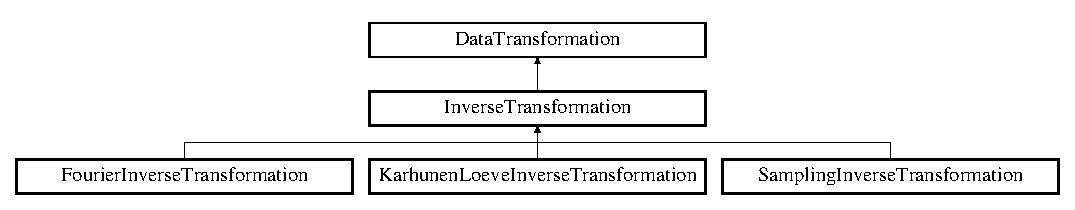
\includegraphics[height=2.372881cm]{classPecos_1_1InverseTransformation}
\end{center}
\end{figure}
\subsection*{Public Member Functions}
\begin{DoxyCompactItemize}
\item 
\hyperlink{classPecos_1_1InverseTransformation_a2f26b12650822873ec0fd05d7fdcd53c}{Inverse\+Transformation} ()\label{classPecos_1_1InverseTransformation_a2f26b12650822873ec0fd05d7fdcd53c}

\begin{DoxyCompactList}\small\item\em constructor \end{DoxyCompactList}\item 
\hyperlink{classPecos_1_1InverseTransformation_af364ba2a4996b223d946a4e19cd7bc4f}{$\sim$\+Inverse\+Transformation} ()\label{classPecos_1_1InverseTransformation_af364ba2a4996b223d946a4e19cd7bc4f}

\begin{DoxyCompactList}\small\item\em destructor \end{DoxyCompactList}\end{DoxyCompactItemize}
\subsection*{Protected Member Functions}
\begin{DoxyCompactItemize}
\item 
void \hyperlink{classPecos_1_1InverseTransformation_aff7310eaa8322a3eccf9815cc7da4a8e}{initialize} (const Real \&total\+\_\+t, const Real \&w\+\_\+bar, size\+\_\+t seed)\label{classPecos_1_1InverseTransformation_aff7310eaa8322a3eccf9815cc7da4a8e}

\begin{DoxyCompactList}\small\item\em set scalar data \end{DoxyCompactList}\item 
void \hyperlink{classPecos_1_1InverseTransformation_a2f54b6bae76157d4a964cd3ff73e4947}{power\+\_\+spectral\+\_\+density} (const String \&psd\+\_\+name, const Real \&param=0.)\label{classPecos_1_1InverseTransformation_a2f54b6bae76157d4a964cd3ff73e4947}

\begin{DoxyCompactList}\small\item\em set P\+SD to standard embedded function \end{DoxyCompactList}\item 
void \hyperlink{classPecos_1_1InverseTransformation_a97ff15b18230b747c64cde3596a1d6f3}{power\+\_\+spectral\+\_\+density} (const Real\+Real\+Pair\+Array \&psd)
\end{DoxyCompactItemize}
\subsection*{Protected Attributes}
\begin{DoxyCompactItemize}
\item 
Real \hyperlink{classPecos_1_1InverseTransformation_a0b7e8700325688780b8907292cfc581d}{total\+Time}\label{classPecos_1_1InverseTransformation_a0b7e8700325688780b8907292cfc581d}

\begin{DoxyCompactList}\small\item\em total time window \end{DoxyCompactList}\item 
Real \hyperlink{classPecos_1_1InverseTransformation_a76b36c18f595ebb232d960272004e2cf}{delta\+Time}\label{classPecos_1_1InverseTransformation_a76b36c18f595ebb232d960272004e2cf}

\begin{DoxyCompactList}\small\item\em time increment \end{DoxyCompactList}\item 
Real\+Vector \hyperlink{classPecos_1_1InverseTransformation_a2d9d6c6e9be9cbe8504e5193a2bfb44f}{time\+Sequence}\label{classPecos_1_1InverseTransformation_a2d9d6c6e9be9cbe8504e5193a2bfb44f}

\begin{DoxyCompactList}\small\item\em discretized time sequence \end{DoxyCompactList}\item 
Real \hyperlink{classPecos_1_1InverseTransformation_ae58b738711bb39b110ee92f41852a088}{omega\+Bar}\label{classPecos_1_1InverseTransformation_ae58b738711bb39b110ee92f41852a088}

\begin{DoxyCompactList}\small\item\em cut-\/off frequency (rad/s) \end{DoxyCompactList}\item 
Real \hyperlink{classPecos_1_1InverseTransformation_a4733a45fbc8d43aa632eca62dfa11694}{delta\+Omega}\label{classPecos_1_1InverseTransformation_a4733a45fbc8d43aa632eca62dfa11694}

\begin{DoxyCompactList}\small\item\em frequency increment (rad/s) \end{DoxyCompactList}\item 
Real\+Vector \hyperlink{classPecos_1_1InverseTransformation_a0b7820a4e99c52ee3a7243174371bef2}{omega\+Sequence}\label{classPecos_1_1InverseTransformation_a0b7820a4e99c52ee3a7243174371bef2}

\begin{DoxyCompactList}\small\item\em discretized frequency sequence \end{DoxyCompactList}\item 
Real\+Vector \hyperlink{classPecos_1_1InverseTransformation_a6581c2dbbad535c9fc176635dfbbf709}{psd\+Sequence}\label{classPecos_1_1InverseTransformation_a6581c2dbbad535c9fc176635dfbbf709}

\begin{DoxyCompactList}\small\item\em P\+SD sequence (frequency domain) \end{DoxyCompactList}\item 
\hyperlink{classPecos_1_1LHSDriver}{L\+H\+S\+Driver} \hyperlink{classPecos_1_1InverseTransformation_a00989baaeba2eacae4fb147c47d04f1f}{lhs\+Sampler}\label{classPecos_1_1InverseTransformation_a00989baaeba2eacae4fb147c47d04f1f}

\begin{DoxyCompactList}\small\item\em L\+HS wrapper for generating normal or uniform sample sets. \end{DoxyCompactList}\item 
Real\+Vector \hyperlink{classPecos_1_1InverseTransformation_a17018c54acd67607b74c8783997d43a9}{inverse\+Sample}\label{classPecos_1_1InverseTransformation_a17018c54acd67607b74c8783997d43a9}

\begin{DoxyCompactList}\small\item\em a single computed inverse sample (time domain) \end{DoxyCompactList}\item 
Real\+Matrix \hyperlink{classPecos_1_1InverseTransformation_ab9922b4f4d5024622225f70ea343f9ee}{inverse\+Samples}\label{classPecos_1_1InverseTransformation_ab9922b4f4d5024622225f70ea343f9ee}

\begin{DoxyCompactList}\small\item\em a computed set of inverse samples (time domain) \end{DoxyCompactList}\end{DoxyCompactItemize}


\subsection{Detailed Description}
Class for inverse data transformation. 

The \hyperlink{classPecos_1_1InverseTransformation}{Inverse\+Transformation} employs an inverse transform to map from the frequency domain to the time domain. 

\subsection{Member Function Documentation}
\index{Pecos\+::\+Inverse\+Transformation@{Pecos\+::\+Inverse\+Transformation}!power\+\_\+spectral\+\_\+density@{power\+\_\+spectral\+\_\+density}}
\index{power\+\_\+spectral\+\_\+density@{power\+\_\+spectral\+\_\+density}!Pecos\+::\+Inverse\+Transformation@{Pecos\+::\+Inverse\+Transformation}}
\subsubsection[{\texorpdfstring{power\+\_\+spectral\+\_\+density(const Real\+Real\+Pair\+Array \&psd)}{power_spectral_density(const RealRealPairArray &psd)}}]{\setlength{\rightskip}{0pt plus 5cm}void power\+\_\+spectral\+\_\+density (
\begin{DoxyParamCaption}
\item[{const Real\+Real\+Pair\+Array \&}]{psd}
\end{DoxyParamCaption}
)\hspace{0.3cm}{\ttfamily [protected]}}\label{classPecos_1_1InverseTransformation_a97ff15b18230b747c64cde3596a1d6f3}
Incoming psd if a set of (x,y) pairs that define a P\+SD curve (w, g(w)). The incoming discretization cannot be assumed to match that selected for psd\+Sequence; therefore, linear interpolation is performed in any combination of log or linear scales for the two axes. 

The documentation for this class was generated from the following files\+:\begin{DoxyCompactItemize}
\item 
Inverse\+Transformation.\+hpp\item 
Inverse\+Transformation.\+cpp\end{DoxyCompactItemize}

\section{Inv\+Gamma\+Random\+Variable Class Reference}
\label{classPecos_1_1InvGammaRandomVariable}\index{Inv\+Gamma\+Random\+Variable@{Inv\+Gamma\+Random\+Variable}}


Derived random variable class for gamma random variables.  


Inheritance diagram for Inv\+Gamma\+Random\+Variable\+:\begin{figure}[H]
\begin{center}
\leavevmode
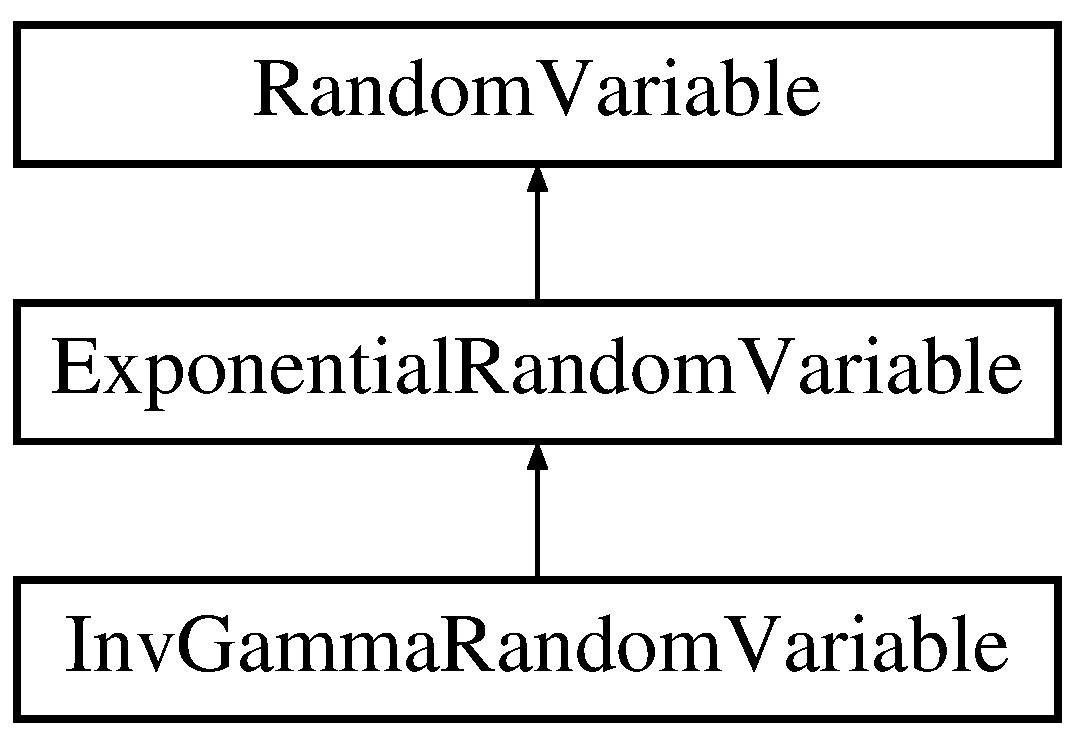
\includegraphics[height=3.000000cm]{classPecos_1_1InvGammaRandomVariable}
\end{center}
\end{figure}
\subsection*{Public Member Functions}
\begin{DoxyCompactItemize}
\item 
\hyperlink{classPecos_1_1InvGammaRandomVariable_a556029c5f42f838a84ed3a5c1371b2f0}{Inv\+Gamma\+Random\+Variable} ()\label{classPecos_1_1InvGammaRandomVariable_a556029c5f42f838a84ed3a5c1371b2f0}

\begin{DoxyCompactList}\small\item\em default constructor \end{DoxyCompactList}\item 
\hyperlink{classPecos_1_1InvGammaRandomVariable_a2d8ac3544ef1d95599584ad31201d514}{Inv\+Gamma\+Random\+Variable} (Real alpha, Real beta)\label{classPecos_1_1InvGammaRandomVariable_a2d8ac3544ef1d95599584ad31201d514}

\begin{DoxyCompactList}\small\item\em alternate constructor \end{DoxyCompactList}\item 
\hyperlink{classPecos_1_1InvGammaRandomVariable_ae4497f12cdcee76874463188097d526b}{$\sim$\+Inv\+Gamma\+Random\+Variable} ()\label{classPecos_1_1InvGammaRandomVariable_ae4497f12cdcee76874463188097d526b}

\begin{DoxyCompactList}\small\item\em destructor \end{DoxyCompactList}\item 
Real \hyperlink{classPecos_1_1InvGammaRandomVariable_addd564e7f4f314e12d38df74d845f0d8}{cdf} (Real x) const \label{classPecos_1_1InvGammaRandomVariable_addd564e7f4f314e12d38df74d845f0d8}

\begin{DoxyCompactList}\small\item\em return the cumulative distribution function value of the random variable at x \end{DoxyCompactList}\item 
Real \hyperlink{classPecos_1_1InvGammaRandomVariable_a23c3b599e7e4788a9a5e9e93c3dbaf4d}{ccdf} (Real x) const \label{classPecos_1_1InvGammaRandomVariable_a23c3b599e7e4788a9a5e9e93c3dbaf4d}

\begin{DoxyCompactList}\small\item\em return the complementary cumulative distribution function value of the random variable at x \end{DoxyCompactList}\item 
Real \hyperlink{classPecos_1_1InvGammaRandomVariable_a918a1aac05ca349ea5313eebcba46c3e}{inverse\+\_\+cdf} (Real p\+\_\+cdf) const \label{classPecos_1_1InvGammaRandomVariable_a918a1aac05ca349ea5313eebcba46c3e}

\begin{DoxyCompactList}\small\item\em return the x value corresponding to a cumulative probability \end{DoxyCompactList}\item 
Real \hyperlink{classPecos_1_1InvGammaRandomVariable_afda003a1f59ff6930902cd5c8601f49b}{inverse\+\_\+ccdf} (Real p\+\_\+ccdf) const \label{classPecos_1_1InvGammaRandomVariable_afda003a1f59ff6930902cd5c8601f49b}

\begin{DoxyCompactList}\small\item\em return the x value corresponding to a complementary cumulative probability \end{DoxyCompactList}\item 
Real \hyperlink{classPecos_1_1InvGammaRandomVariable_a8ec69265f428e17c1707133cb137a819}{pdf} (Real x) const \label{classPecos_1_1InvGammaRandomVariable_a8ec69265f428e17c1707133cb137a819}

\begin{DoxyCompactList}\small\item\em return the value of the random variable\textquotesingle{}s probability density function at x \end{DoxyCompactList}\item 
Real \hyperlink{classPecos_1_1InvGammaRandomVariable_aaa7ca3718abc034be7629af5594efca0}{pdf\+\_\+gradient} (Real x) const \label{classPecos_1_1InvGammaRandomVariable_aaa7ca3718abc034be7629af5594efca0}

\begin{DoxyCompactList}\small\item\em return the gradient of the random variable\textquotesingle{}s probability density function at x \end{DoxyCompactList}\item 
Real \hyperlink{classPecos_1_1InvGammaRandomVariable_a514a0abe97269ac6e003f43683d9137e}{pdf\+\_\+hessian} (Real x) const \label{classPecos_1_1InvGammaRandomVariable_a514a0abe97269ac6e003f43683d9137e}

\begin{DoxyCompactList}\small\item\em return the hessian of the random variable\textquotesingle{}s probability density function at x \end{DoxyCompactList}\item 
Real \hyperlink{classPecos_1_1InvGammaRandomVariable_a6e2b6b6f13eedb2eb1ef3bc455a06392}{log\+\_\+pdf} (Real x) const \label{classPecos_1_1InvGammaRandomVariable_a6e2b6b6f13eedb2eb1ef3bc455a06392}

\begin{DoxyCompactList}\small\item\em return the value of the natural log of the random variable\textquotesingle{}s probability density function at x (useful for calculations of log density in Bayesian methods) \end{DoxyCompactList}\item 
Real \hyperlink{classPecos_1_1InvGammaRandomVariable_a5ccc16c04690f0c501f44c1ffae2bbd1}{log\+\_\+pdf\+\_\+gradient} (Real x) const \label{classPecos_1_1InvGammaRandomVariable_a5ccc16c04690f0c501f44c1ffae2bbd1}

\begin{DoxyCompactList}\small\item\em return the gradient of the natural log of the random variable\textquotesingle{}s probability density function at x (useful for defining M\+C\+MC proposal distributions in Bayesian methods) \end{DoxyCompactList}\item 
Real \hyperlink{classPecos_1_1InvGammaRandomVariable_a7b43f26f0f2bcdfef15d87e1f9399b33}{log\+\_\+pdf\+\_\+hessian} (Real x) const \label{classPecos_1_1InvGammaRandomVariable_a7b43f26f0f2bcdfef15d87e1f9399b33}

\begin{DoxyCompactList}\small\item\em return the Hessian of the natural log of the random variable\textquotesingle{}s probability density function at x (useful for defining M\+C\+MC proposal distributions in Bayesian methods) \end{DoxyCompactList}\item 
Real \hyperlink{classPecos_1_1InvGammaRandomVariable_acffcd338a207168a147fffe0778ccf3c}{inverse\+\_\+standard\+\_\+cdf} (Real p\+\_\+cdf) const \label{classPecos_1_1InvGammaRandomVariable_acffcd338a207168a147fffe0778ccf3c}

\begin{DoxyCompactList}\small\item\em return the x value for a standardized probability distribution corresponding to a cumulative probability \end{DoxyCompactList}\item 
Real \hyperlink{classPecos_1_1InvGammaRandomVariable_a206a02581b82f44be4a5321488a12daa}{standard\+\_\+pdf} (Real z) const \label{classPecos_1_1InvGammaRandomVariable_a206a02581b82f44be4a5321488a12daa}

\begin{DoxyCompactList}\small\item\em return the value of a standardized random variable\textquotesingle{}s probability density function at x \end{DoxyCompactList}\item 
Real \hyperlink{classPecos_1_1InvGammaRandomVariable_a1eb7deb350fc38d35e32ba7d0b96c464}{log\+\_\+standard\+\_\+pdf} (Real z) const \label{classPecos_1_1InvGammaRandomVariable_a1eb7deb350fc38d35e32ba7d0b96c464}

\begin{DoxyCompactList}\small\item\em return the natural log of a standardized random variable\textquotesingle{}s probability density function at x (useful for calculations of log density in Bayesian methods) \end{DoxyCompactList}\item 
Real \hyperlink{classPecos_1_1InvGammaRandomVariable_a73ea75d51f5415f600bebbca4a9628b7}{log\+\_\+standard\+\_\+pdf\+\_\+gradient} (Real z) const \label{classPecos_1_1InvGammaRandomVariable_a73ea75d51f5415f600bebbca4a9628b7}

\begin{DoxyCompactList}\small\item\em return the gradient of the natural log of a standardized random variable\textquotesingle{}s probability density function at x (useful for calculations of log density in Bayesian methods) \end{DoxyCompactList}\item 
Real \hyperlink{classPecos_1_1InvGammaRandomVariable_acf89562740c674e54901e97817f56b69}{log\+\_\+standard\+\_\+pdf\+\_\+hessian} (Real z) const \label{classPecos_1_1InvGammaRandomVariable_acf89562740c674e54901e97817f56b69}

\begin{DoxyCompactList}\small\item\em return the Hessian of the natural log of a standardized random variable\textquotesingle{}s probability density function at x (useful for calculations of log density in Bayesian methods) \end{DoxyCompactList}\item 
Real \hyperlink{classPecos_1_1InvGammaRandomVariable_aa891dab1ae9a225f493e3a0e5032b778}{parameter} (short dist\+\_\+param) const \label{classPecos_1_1InvGammaRandomVariable_aa891dab1ae9a225f493e3a0e5032b778}

\begin{DoxyCompactList}\small\item\em return the value of the named distribution parameter \end{DoxyCompactList}\item 
void \hyperlink{classPecos_1_1InvGammaRandomVariable_ae8e123224f588aee676d5d56d5ca900d}{parameter} (short dist\+\_\+param, Real val)\label{classPecos_1_1InvGammaRandomVariable_ae8e123224f588aee676d5d56d5ca900d}

\begin{DoxyCompactList}\small\item\em update the value of the named distribution parameter \end{DoxyCompactList}\item 
Real \hyperlink{classPecos_1_1InvGammaRandomVariable_a962ffe5a3593be370d5c883365c060f4}{mean} () const \label{classPecos_1_1InvGammaRandomVariable_a962ffe5a3593be370d5c883365c060f4}

\begin{DoxyCompactList}\small\item\em return the distribution mean \end{DoxyCompactList}\item 
Real \hyperlink{classPecos_1_1InvGammaRandomVariable_ae1fff19ce29a79d657043a598523635d}{median} () const \label{classPecos_1_1InvGammaRandomVariable_ae1fff19ce29a79d657043a598523635d}

\begin{DoxyCompactList}\small\item\em return the distribution mode \end{DoxyCompactList}\item 
Real \hyperlink{classPecos_1_1InvGammaRandomVariable_a72d3d6926edd929cb3f8e12baa655f70}{mode} () const \label{classPecos_1_1InvGammaRandomVariable_a72d3d6926edd929cb3f8e12baa655f70}

\begin{DoxyCompactList}\small\item\em return the distribution mode \end{DoxyCompactList}\item 
Real \hyperlink{classPecos_1_1InvGammaRandomVariable_a6a4ed9624d511f8a4e4f509c82cb0706}{standard\+\_\+deviation} () const \label{classPecos_1_1InvGammaRandomVariable_a6a4ed9624d511f8a4e4f509c82cb0706}

\begin{DoxyCompactList}\small\item\em return the distribution variance \end{DoxyCompactList}\item 
Real \hyperlink{classPecos_1_1InvGammaRandomVariable_a4b8b05b2a9af92dad9cc304c2925a4eb}{variance} () const \label{classPecos_1_1InvGammaRandomVariable_a4b8b05b2a9af92dad9cc304c2925a4eb}

\begin{DoxyCompactList}\small\item\em return the distribution variance \end{DoxyCompactList}\item 
Real \hyperlink{classPecos_1_1InvGammaRandomVariable_a9ee48b3ca93459136b2e73f77873c4aa}{correlation\+\_\+warping\+\_\+factor} (const \hyperlink{classPecos_1_1RandomVariable}{Random\+Variable} \&rv, Real corr) const \label{classPecos_1_1InvGammaRandomVariable_a9ee48b3ca93459136b2e73f77873c4aa}

\begin{DoxyCompactList}\small\item\em compute the warping factor for correlation between the current variable and the one passed in (used in \hyperlink{classPecos_1_1NatafTransformation}{Nataf\+Transformation}) \end{DoxyCompactList}\item 
Real \hyperlink{classPecos_1_1InvGammaRandomVariable_af889af8adfb262c9b74f573b2a9ffc99}{dx\+\_\+ds} (short dist\+\_\+param, short u\+\_\+type, Real x, Real z) const 
\item 
Real \hyperlink{classPecos_1_1InvGammaRandomVariable_af6b5fc528523180bed5fc3008dcea205}{dz\+\_\+ds\+\_\+factor} (short u\+\_\+type, Real x, Real z) const 
\item 
void {\bfseries update} (Real alpha, Real beta)\label{classPecos_1_1InvGammaRandomVariable_aaa82eccfdca4d440a4e2d4a890b0d9ed}

\end{DoxyCompactItemize}
\subsection*{Static Public Member Functions}
\begin{DoxyCompactItemize}
\item 
static Real {\bfseries pdf} (Real x, Real alpha, Real beta)\label{classPecos_1_1InvGammaRandomVariable_a739d94cef9ee188f00056e229ca3fd95}

\item 
static Real {\bfseries cdf} (Real x, Real alpha, Real beta)\label{classPecos_1_1InvGammaRandomVariable_a6ccc276bca2bfdfd6f320c65a6c8aaf7}

\item 
static Real {\bfseries inverse\+\_\+cdf} (Real \hyperlink{classPecos_1_1InvGammaRandomVariable_addd564e7f4f314e12d38df74d845f0d8}{cdf}, Real alpha, Real beta)\label{classPecos_1_1InvGammaRandomVariable_a2e77b37ec653326d8c6189a646b8db7b}

\item 
static void {\bfseries moments\+\_\+from\+\_\+params} (Real alpha, Real beta, Real \&\hyperlink{classPecos_1_1InvGammaRandomVariable_a962ffe5a3593be370d5c883365c060f4}{mean}, Real \&std\+\_\+dev)\label{classPecos_1_1InvGammaRandomVariable_af6459b831a8e62a41f7eab34d06edad8}

\end{DoxyCompactItemize}
\subsection*{Protected Member Functions}
\begin{DoxyCompactItemize}
\item 
void \hyperlink{classPecos_1_1InvGammaRandomVariable_aaa6750cbee2245416a6eeeac58d4405a}{update\+\_\+boost} ()\label{classPecos_1_1InvGammaRandomVariable_aaa6750cbee2245416a6eeeac58d4405a}

\begin{DoxyCompactList}\small\item\em create a new inv\+Gamma\+Dist instance \end{DoxyCompactList}\end{DoxyCompactItemize}
\subsection*{Protected Attributes}
\begin{DoxyCompactItemize}
\item 
Real \hyperlink{classPecos_1_1InvGammaRandomVariable_af2fa8d657b4ae8750d30b09f10760799}{alpha\+Shape}\label{classPecos_1_1InvGammaRandomVariable_af2fa8d657b4ae8750d30b09f10760799}

\begin{DoxyCompactList}\small\item\em alpha shape parameter of inverse gamma random variable (statistical P\+DF convention; differs from Gen\+Laguerre polynomial convention) \end{DoxyCompactList}\item 
inv\+\_\+gamma\+\_\+dist $\ast$ \hyperlink{classPecos_1_1InvGammaRandomVariable_ada70ebb3be086d76c24fa4d684aca901}{inv\+Gamma\+Dist}\label{classPecos_1_1InvGammaRandomVariable_ada70ebb3be086d76c24fa4d684aca901}

\begin{DoxyCompactList}\small\item\em pointer to the Boost inv\+\_\+gamma\+\_\+dist instance \end{DoxyCompactList}\end{DoxyCompactItemize}


\subsection{Detailed Description}
Derived random variable class for gamma random variables. 

Manages alpha\+Shape and inherits beta\+Scale. This follows the definition at \href{https://en.wikipedia.org/wiki/Inverse-gamma_distribution}{\tt https\+://en.\+wikipedia.\+org/wiki/\+Inverse-\/gamma\+\_\+distribution}. This implementation also supports a standard inverse-\/gamma with beta = 1. 

\subsection{Member Function Documentation}
\index{Pecos\+::\+Inv\+Gamma\+Random\+Variable@{Pecos\+::\+Inv\+Gamma\+Random\+Variable}!dx\+\_\+ds@{dx\+\_\+ds}}
\index{dx\+\_\+ds@{dx\+\_\+ds}!Pecos\+::\+Inv\+Gamma\+Random\+Variable@{Pecos\+::\+Inv\+Gamma\+Random\+Variable}}
\subsubsection[{\texorpdfstring{dx\+\_\+ds(short dist\+\_\+param, short u\+\_\+type, Real x, Real z) const }{dx_ds(short dist_param, short u_type, Real x, Real z) const }}]{\setlength{\rightskip}{0pt plus 5cm}Real dx\+\_\+ds (
\begin{DoxyParamCaption}
\item[{short}]{dist\+\_\+param, }
\item[{short}]{u\+\_\+type, }
\item[{Real}]{x, }
\item[{Real}]{z}
\end{DoxyParamCaption}
) const\hspace{0.3cm}{\ttfamily [inline]}, {\ttfamily [virtual]}}\label{classPecos_1_1InvGammaRandomVariable_af889af8adfb262c9b74f573b2a9ffc99}
dx/ds is derived by differentiating \hyperlink{classPecos_1_1NatafTransformation_a5feeecf846fc017c5a28eccb4e955dc1}{Nataf\+Transformation\+::trans\+\_\+\+Z\+\_\+to\+\_\+\+X()} with respect to distribution parameter s. dz/ds is zero if uncorrelated, while \hyperlink{classPecos_1_1InvGammaRandomVariable_af6b5fc528523180bed5fc3008dcea205}{dz\+\_\+ds\+\_\+factor()} manages contributions in the correlated case. 

Reimplemented from \hyperlink{classPecos_1_1ExponentialRandomVariable_af889af8adfb262c9b74f573b2a9ffc99}{Exponential\+Random\+Variable}.



References Inv\+Gamma\+Random\+Variable\+::dz\+\_\+ds\+\_\+factor().



Referenced by Inv\+Gamma\+Random\+Variable\+::correlation\+\_\+warping\+\_\+factor().

\index{Pecos\+::\+Inv\+Gamma\+Random\+Variable@{Pecos\+::\+Inv\+Gamma\+Random\+Variable}!dz\+\_\+ds\+\_\+factor@{dz\+\_\+ds\+\_\+factor}}
\index{dz\+\_\+ds\+\_\+factor@{dz\+\_\+ds\+\_\+factor}!Pecos\+::\+Inv\+Gamma\+Random\+Variable@{Pecos\+::\+Inv\+Gamma\+Random\+Variable}}
\subsubsection[{\texorpdfstring{dz\+\_\+ds\+\_\+factor(short u\+\_\+type, Real x, Real z) const }{dz_ds_factor(short u_type, Real x, Real z) const }}]{\setlength{\rightskip}{0pt plus 5cm}Real dz\+\_\+ds\+\_\+factor (
\begin{DoxyParamCaption}
\item[{short}]{u\+\_\+type, }
\item[{Real}]{x, }
\item[{Real}]{z}
\end{DoxyParamCaption}
) const\hspace{0.3cm}{\ttfamily [inline]}, {\ttfamily [virtual]}}\label{classPecos_1_1InvGammaRandomVariable_af6b5fc528523180bed5fc3008dcea205}
dx/ds is derived by differentiating \hyperlink{classPecos_1_1NatafTransformation_a5feeecf846fc017c5a28eccb4e955dc1}{Nataf\+Transformation\+::trans\+\_\+\+Z\+\_\+to\+\_\+\+X()} with respect to distribution parameter s. For the uncorrelated case, u and z are constants. For the correlated case, u is a constant, but z(s) = L(s) u due to Nataf dependence on s and dz/ds = d\+L/ds u. 

Reimplemented from \hyperlink{classPecos_1_1ExponentialRandomVariable_af6b5fc528523180bed5fc3008dcea205}{Exponential\+Random\+Variable}.



Referenced by Inv\+Gamma\+Random\+Variable\+::dx\+\_\+ds().



The documentation for this class was generated from the following file\+:\begin{DoxyCompactItemize}
\item 
Inv\+Gamma\+Random\+Variable.\+hpp\end{DoxyCompactItemize}

\section{Iterator Class Reference}
\label{classIterator}\index{Iterator@{Iterator}}


The base class for all parallel iterators.  




\subsection{Detailed Description}
The base class for all parallel iterators. 

The documentation for this class was generated from the following file\+:\begin{DoxyCompactItemize}
\item 
Runtime\+Environment.\+hpp\end{DoxyCompactItemize}

\section{Jacobi\+Orthog\+Polynomial Class Reference}
\label{classPecos_1_1JacobiOrthogPolynomial}\index{Jacobi\+Orthog\+Polynomial@{Jacobi\+Orthog\+Polynomial}}


Derived orthogonal polynomial class for Jacobi polynomials.  


Inheritance diagram for Jacobi\+Orthog\+Polynomial\+:\begin{figure}[H]
\begin{center}
\leavevmode
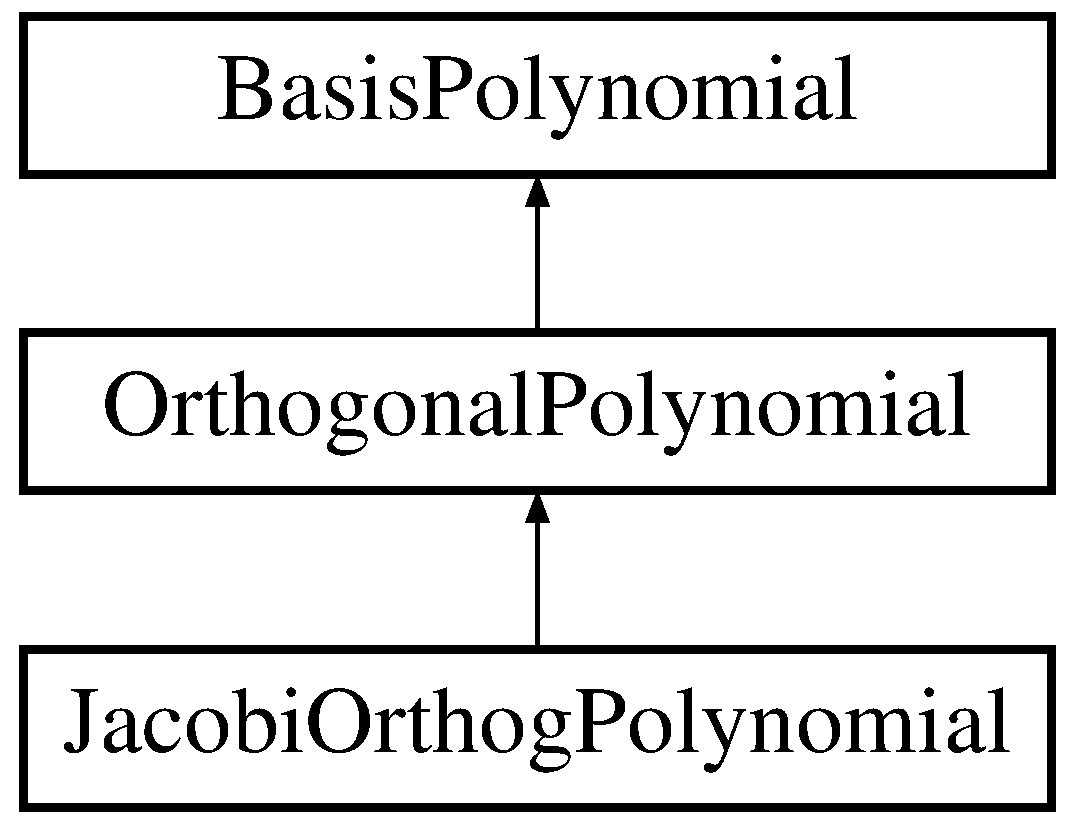
\includegraphics[height=3.000000cm]{classPecos_1_1JacobiOrthogPolynomial}
\end{center}
\end{figure}
\subsection*{Public Member Functions}
\begin{DoxyCompactItemize}
\item 
\hyperlink{classPecos_1_1JacobiOrthogPolynomial_ae53de420db30554be0b6b9623d78e2ae}{Jacobi\+Orthog\+Polynomial} ()\label{classPecos_1_1JacobiOrthogPolynomial_ae53de420db30554be0b6b9623d78e2ae}

\begin{DoxyCompactList}\small\item\em default constructor \end{DoxyCompactList}\item 
\hyperlink{classPecos_1_1JacobiOrthogPolynomial_a9127969c07687bdf1857dc2f6627f20c}{Jacobi\+Orthog\+Polynomial} (Real \hyperlink{classPecos_1_1JacobiOrthogPolynomial_aeeb4ce11a8d413209be1ec08eced8728}{alpha\+\_\+stat}, Real \hyperlink{classPecos_1_1JacobiOrthogPolynomial_a7f9584e538ee1574bd4d8d1afb622ed6}{beta\+\_\+stat})\label{classPecos_1_1JacobiOrthogPolynomial_a9127969c07687bdf1857dc2f6627f20c}

\begin{DoxyCompactList}\small\item\em standard constructor \end{DoxyCompactList}\item 
\hyperlink{classPecos_1_1JacobiOrthogPolynomial_a072925a371f3ffdb7bf334e3ac768a87}{$\sim$\+Jacobi\+Orthog\+Polynomial} ()\label{classPecos_1_1JacobiOrthogPolynomial_a072925a371f3ffdb7bf334e3ac768a87}

\begin{DoxyCompactList}\small\item\em destructor \end{DoxyCompactList}\item 
Real \hyperlink{classPecos_1_1JacobiOrthogPolynomial_acc5475d6b992e443e3cce753a48cfc32}{weight\+\_\+factor} ()\label{classPecos_1_1JacobiOrthogPolynomial_acc5475d6b992e443e3cce753a48cfc32}

\begin{DoxyCompactList}\small\item\em calculate and return wt\+Factor based on alpha\+Poly and beta\+Poly \end{DoxyCompactList}\end{DoxyCompactItemize}
\subsection*{Protected Member Functions}
\begin{DoxyCompactItemize}
\item 
Real \hyperlink{classPecos_1_1JacobiOrthogPolynomial_a8792a858ac05a2158880e876f9da2019}{type1\+\_\+value} (Real x, unsigned short order)
\begin{DoxyCompactList}\small\item\em retrieve the value of the n\+\_\+th type 1 polynomial for a given parameter x using traditional characteristic polynomial formulation \end{DoxyCompactList}\item 
Real \hyperlink{classPecos_1_1JacobiOrthogPolynomial_aac6751aa35bf5fcb42c520a322fc26dc}{type1\+\_\+gradient} (Real x, unsigned short order)
\begin{DoxyCompactList}\small\item\em retrieve the gradient of the n\+\_\+th type 1 polynomial for a given parameter x using traditional characteristic polynomial formulation \end{DoxyCompactList}\item 
Real \hyperlink{classPecos_1_1JacobiOrthogPolynomial_ae957c8c2e7ea13728bafbad0c9b2996e}{type1\+\_\+hessian} (Real x, unsigned short order)
\begin{DoxyCompactList}\small\item\em retrieve the Hessian of the n\+\_\+th type 1 polynomial for a given parameter x using traditional characteristic polynomial formulation \end{DoxyCompactList}\item 
Real \hyperlink{classPecos_1_1JacobiOrthogPolynomial_a77c0dbb874af1190d448d01da6efbe4e}{norm\+\_\+squared} (unsigned short order)
\begin{DoxyCompactList}\small\item\em returns the norm-\/squared of the n\+\_\+th order polynomial defined by the inner product $<$Poly\+\_\+n, Poly\+\_\+n$>$ = $\vert$$\vert$\+Poly\+\_\+n$\vert$$\vert$$^\wedge$2 \end{DoxyCompactList}\item 
const Real\+Array \& \hyperlink{classPecos_1_1JacobiOrthogPolynomial_a10873b28f1284aff4ea214e00c4f86dd}{collocation\+\_\+points} (unsigned short order)
\begin{DoxyCompactList}\small\item\em return collocation points corresponding to orthogonal polynomial order n \end{DoxyCompactList}\item 
const Real\+Array \& \hyperlink{classPecos_1_1JacobiOrthogPolynomial_aa010321cf47465dca5725fa15ba58bf6}{type1\+\_\+collocation\+\_\+weights} (unsigned short order)
\begin{DoxyCompactList}\small\item\em return the type 1 collocation weights corresponding to a point set of size order \end{DoxyCompactList}\item 
Real \hyperlink{classPecos_1_1JacobiOrthogPolynomial_a997bdeddf670667c476513fcacc779ca}{alpha\+\_\+polynomial} () const \label{classPecos_1_1JacobiOrthogPolynomial_a997bdeddf670667c476513fcacc779ca}

\begin{DoxyCompactList}\small\item\em return alpha\+Poly \end{DoxyCompactList}\item 
Real \hyperlink{classPecos_1_1JacobiOrthogPolynomial_a22bfc4209dec76716ef51648e945469a}{beta\+\_\+polynomial} () const \label{classPecos_1_1JacobiOrthogPolynomial_a22bfc4209dec76716ef51648e945469a}

\begin{DoxyCompactList}\small\item\em return beta\+Poly \end{DoxyCompactList}\item 
void \hyperlink{classPecos_1_1JacobiOrthogPolynomial_aeeb4ce11a8d413209be1ec08eced8728}{alpha\+\_\+stat} (Real alpha)\label{classPecos_1_1JacobiOrthogPolynomial_aeeb4ce11a8d413209be1ec08eced8728}

\begin{DoxyCompactList}\small\item\em set beta\+Poly using the conversion beta\+Poly = alpha\+\_\+stat -\/ 1. \end{DoxyCompactList}\item 
void \hyperlink{classPecos_1_1JacobiOrthogPolynomial_a7f9584e538ee1574bd4d8d1afb622ed6}{beta\+\_\+stat} (Real beta)\label{classPecos_1_1JacobiOrthogPolynomial_a7f9584e538ee1574bd4d8d1afb622ed6}

\begin{DoxyCompactList}\small\item\em set alpha\+Poly using the conversion alpha\+Poly = beta\+\_\+stat -\/ 1. \end{DoxyCompactList}\item 
bool \hyperlink{classPecos_1_1JacobiOrthogPolynomial_abc2afafc150f648667a41e0ce656b6da}{parameterized} () const \label{classPecos_1_1JacobiOrthogPolynomial_abc2afafc150f648667a41e0ce656b6da}

\begin{DoxyCompactList}\small\item\em override default definition (false) since Jacobi is parameterized \end{DoxyCompactList}\item 
Real \hyperlink{classPecos_1_1JacobiOrthogPolynomial_a8c1e8d014e82efc5a1c20f973b5bc715}{length\+\_\+scale} () const 
\end{DoxyCompactItemize}
\subsection*{Private Attributes}
\begin{DoxyCompactItemize}
\item 
Real \hyperlink{classPecos_1_1JacobiOrthogPolynomial_a11666846719189915a02ac6f1f96e393}{alpha\+Poly}\label{classPecos_1_1JacobiOrthogPolynomial_a11666846719189915a02ac6f1f96e393}

\begin{DoxyCompactList}\small\item\em the alpha parameter for the Jacobi polynomial as defined by Abramowitz and Stegun (differs from statistical P\+DF notation) \end{DoxyCompactList}\item 
Real \hyperlink{classPecos_1_1JacobiOrthogPolynomial_a96c0b0201ca445f95be14ec035b595cb}{beta\+Poly}\label{classPecos_1_1JacobiOrthogPolynomial_a96c0b0201ca445f95be14ec035b595cb}

\begin{DoxyCompactList}\small\item\em the beta parameter for the Jacobi polynomial as defined by Abramowitz and Stegun (differs from statistical P\+DF notation) \end{DoxyCompactList}\end{DoxyCompactItemize}
\subsection*{Additional Inherited Members}


\subsection{Detailed Description}
Derived orthogonal polynomial class for Jacobi polynomials. 

The \hyperlink{classPecos_1_1JacobiOrthogPolynomial}{Jacobi\+Orthog\+Polynomial} class evaluates a univariate Jacobi polynomial P$^\wedge$(alpha,beta)\+\_\+n of a particular order. These polynomials are orthogonal with respect to the weight function (1-\/x)$^\wedge$alpha (1+x)$^\wedge$beta when integrated over the support range of \mbox{[}-\/1,+1\mbox{]}. This corresponds to the probability density function f(x) = (1-\/x)$^\wedge$alpha (1+x)$^\wedge$beta / (2$^\wedge$(alpha+beta+1) B(alpha+1,beta+1)) for the beta distribution for \mbox{[}L,U\mbox{]}=\mbox{[}-\/1,1\mbox{]}, where common statistical P\+DF notation conventions (see, e.\+g., the uncertain variables section in the D\+A\+K\+O\+TA Reference Manual) and the Abramowiz and Stegun orthogonal polynomial conventions are inverted and require conversion in this case (alpha\+\_\+poly = beta\+\_\+stat -\/ 1; beta\+\_\+poly = alpha\+\_\+stat -\/ 1 with the poly definitions used in both cases above). It enables (mixed) multidimensional orthogonal polynomial basis functions within \hyperlink{classPecos_1_1OrthogPolyApproximation}{Orthog\+Poly\+Approximation}. A special case is the \hyperlink{classPecos_1_1LegendreOrthogPolynomial}{Legendre\+Orthog\+Polynomial} (implemented separately), for which alpha\+\_\+poly = beta\+\_\+poly = 0. 

\subsection{Member Function Documentation}
\index{Pecos\+::\+Jacobi\+Orthog\+Polynomial@{Pecos\+::\+Jacobi\+Orthog\+Polynomial}!type1\+\_\+value@{type1\+\_\+value}}
\index{type1\+\_\+value@{type1\+\_\+value}!Pecos\+::\+Jacobi\+Orthog\+Polynomial@{Pecos\+::\+Jacobi\+Orthog\+Polynomial}}
\subsubsection[{\texorpdfstring{type1\+\_\+value(\+Real x, unsigned short order)}{type1_value(Real x, unsigned short order)}}]{\setlength{\rightskip}{0pt plus 5cm}Real type1\+\_\+value (
\begin{DoxyParamCaption}
\item[{Real}]{x, }
\item[{unsigned short}]{n}
\end{DoxyParamCaption}
)\hspace{0.3cm}{\ttfamily [protected]}, {\ttfamily [virtual]}}\label{classPecos_1_1JacobiOrthogPolynomial_a8792a858ac05a2158880e876f9da2019}


retrieve the value of the n\+\_\+th type 1 polynomial for a given parameter x using traditional characteristic polynomial formulation 

For orthogonal polynomials, n specifies the order of the polynomial, whereas for interpolation polynomials, it identifies the interpolant for the n-\/th point. 

Reimplemented from \hyperlink{classPecos_1_1BasisPolynomial_a1fab871e99cec3a1933a2b1e9ed8a625}{Basis\+Polynomial}.



References Jacobi\+Orthog\+Polynomial\+::alpha\+Poly, Jacobi\+Orthog\+Polynomial\+::beta\+Poly, and Basis\+Polynomial\+::pochhammer().



Referenced by Jacobi\+Orthog\+Polynomial\+::type1\+\_\+collocation\+\_\+weights(), and Jacobi\+Orthog\+Polynomial\+::type1\+\_\+gradient().

\index{Pecos\+::\+Jacobi\+Orthog\+Polynomial@{Pecos\+::\+Jacobi\+Orthog\+Polynomial}!type1\+\_\+gradient@{type1\+\_\+gradient}}
\index{type1\+\_\+gradient@{type1\+\_\+gradient}!Pecos\+::\+Jacobi\+Orthog\+Polynomial@{Pecos\+::\+Jacobi\+Orthog\+Polynomial}}
\subsubsection[{\texorpdfstring{type1\+\_\+gradient(\+Real x, unsigned short order)}{type1_gradient(Real x, unsigned short order)}}]{\setlength{\rightskip}{0pt plus 5cm}Real type1\+\_\+gradient (
\begin{DoxyParamCaption}
\item[{Real}]{x, }
\item[{unsigned short}]{n}
\end{DoxyParamCaption}
)\hspace{0.3cm}{\ttfamily [protected]}, {\ttfamily [virtual]}}\label{classPecos_1_1JacobiOrthogPolynomial_aac6751aa35bf5fcb42c520a322fc26dc}


retrieve the gradient of the n\+\_\+th type 1 polynomial for a given parameter x using traditional characteristic polynomial formulation 

For orthogonal polynomials, n specifies the order of the polynomial, whereas for interpolation polynomials, it identifies the interpolant for the n-\/th point. 

Reimplemented from \hyperlink{classPecos_1_1BasisPolynomial_a6f69ec84983f551e7e0e4a18b78b4498}{Basis\+Polynomial}.



References Jacobi\+Orthog\+Polynomial\+::alpha\+Poly, Jacobi\+Orthog\+Polynomial\+::beta\+Poly, Basis\+Polynomial\+::pochhammer(), and Jacobi\+Orthog\+Polynomial\+::type1\+\_\+value().



Referenced by Jacobi\+Orthog\+Polynomial\+::type1\+\_\+collocation\+\_\+weights(), and Jacobi\+Orthog\+Polynomial\+::type1\+\_\+hessian().

\index{Pecos\+::\+Jacobi\+Orthog\+Polynomial@{Pecos\+::\+Jacobi\+Orthog\+Polynomial}!type1\+\_\+hessian@{type1\+\_\+hessian}}
\index{type1\+\_\+hessian@{type1\+\_\+hessian}!Pecos\+::\+Jacobi\+Orthog\+Polynomial@{Pecos\+::\+Jacobi\+Orthog\+Polynomial}}
\subsubsection[{\texorpdfstring{type1\+\_\+hessian(\+Real x, unsigned short order)}{type1_hessian(Real x, unsigned short order)}}]{\setlength{\rightskip}{0pt plus 5cm}Real type1\+\_\+hessian (
\begin{DoxyParamCaption}
\item[{Real}]{x, }
\item[{unsigned short}]{n}
\end{DoxyParamCaption}
)\hspace{0.3cm}{\ttfamily [protected]}, {\ttfamily [virtual]}}\label{classPecos_1_1JacobiOrthogPolynomial_ae957c8c2e7ea13728bafbad0c9b2996e}


retrieve the Hessian of the n\+\_\+th type 1 polynomial for a given parameter x using traditional characteristic polynomial formulation 

For orthogonal polynomials, n specifies the order of the polynomial, whereas for interpolation polynomials, it identifies the interpolant for the n-\/th point. 

Reimplemented from \hyperlink{classPecos_1_1BasisPolynomial_a07d617dad8572dd606371e6c89ab6c35}{Basis\+Polynomial}.



References Jacobi\+Orthog\+Polynomial\+::alpha\+Poly, Jacobi\+Orthog\+Polynomial\+::beta\+Poly, Basis\+Polynomial\+::pochhammer(), and Jacobi\+Orthog\+Polynomial\+::type1\+\_\+gradient().

\index{Pecos\+::\+Jacobi\+Orthog\+Polynomial@{Pecos\+::\+Jacobi\+Orthog\+Polynomial}!norm\+\_\+squared@{norm\+\_\+squared}}
\index{norm\+\_\+squared@{norm\+\_\+squared}!Pecos\+::\+Jacobi\+Orthog\+Polynomial@{Pecos\+::\+Jacobi\+Orthog\+Polynomial}}
\subsubsection[{\texorpdfstring{norm\+\_\+squared(unsigned short order)}{norm_squared(unsigned short order)}}]{\setlength{\rightskip}{0pt plus 5cm}Real norm\+\_\+squared (
\begin{DoxyParamCaption}
\item[{unsigned short}]{n}
\end{DoxyParamCaption}
)\hspace{0.3cm}{\ttfamily [protected]}, {\ttfamily [virtual]}}\label{classPecos_1_1JacobiOrthogPolynomial_a77c0dbb874af1190d448d01da6efbe4e}


returns the norm-\/squared of the n\+\_\+th order polynomial defined by the inner product $<$Poly\+\_\+n, Poly\+\_\+n$>$ = $\vert$$\vert$\+Poly\+\_\+n$\vert$$\vert$$^\wedge$2 

This is defined only for orthogonal polynomials. 

Reimplemented from \hyperlink{classPecos_1_1BasisPolynomial_ab74383be309d74823f2e5e85dad739b2}{Basis\+Polynomial}.



References Jacobi\+Orthog\+Polynomial\+::alpha\+Poly, Jacobi\+Orthog\+Polynomial\+::beta\+Poly, Jacobi\+Orthog\+Polynomial\+::collocation\+\_\+points(), Basis\+Polynomial\+::factorial(), and Basis\+Polynomial\+::pochhammer().



Referenced by Jacobi\+Orthog\+Polynomial\+::type1\+\_\+collocation\+\_\+weights().

\index{Pecos\+::\+Jacobi\+Orthog\+Polynomial@{Pecos\+::\+Jacobi\+Orthog\+Polynomial}!collocation\+\_\+points@{collocation\+\_\+points}}
\index{collocation\+\_\+points@{collocation\+\_\+points}!Pecos\+::\+Jacobi\+Orthog\+Polynomial@{Pecos\+::\+Jacobi\+Orthog\+Polynomial}}
\subsubsection[{\texorpdfstring{collocation\+\_\+points(unsigned short order)}{collocation_points(unsigned short order)}}]{\setlength{\rightskip}{0pt plus 5cm}const Real\+Array \& collocation\+\_\+points (
\begin{DoxyParamCaption}
\item[{unsigned short}]{n}
\end{DoxyParamCaption}
)\hspace{0.3cm}{\ttfamily [protected]}, {\ttfamily [virtual]}}\label{classPecos_1_1JacobiOrthogPolynomial_a10873b28f1284aff4ea214e00c4f86dd}


return collocation points corresponding to orthogonal polynomial order n 

This is defined for orthogonal and piecewise interpolation polynomials. 

Reimplemented from \hyperlink{classPecos_1_1BasisPolynomial_a0f96bd4e27ddc5c44117e7b68744b5a4}{Basis\+Polynomial}.



References Jacobi\+Orthog\+Polynomial\+::alpha\+Poly, Jacobi\+Orthog\+Polynomial\+::beta\+Poly, Orthogonal\+Polynomial\+::colloc\+Points, Orthogonal\+Polynomial\+::colloc\+Weights, Jacobi\+Orthog\+Polynomial\+::type1\+\_\+collocation\+\_\+weights(), and Jacobi\+Orthog\+Polynomial\+::weight\+\_\+factor().



Referenced by Jacobi\+Orthog\+Polynomial\+::norm\+\_\+squared(), and Jacobi\+Orthog\+Polynomial\+::type1\+\_\+collocation\+\_\+weights().

\index{Pecos\+::\+Jacobi\+Orthog\+Polynomial@{Pecos\+::\+Jacobi\+Orthog\+Polynomial}!type1\+\_\+collocation\+\_\+weights@{type1\+\_\+collocation\+\_\+weights}}
\index{type1\+\_\+collocation\+\_\+weights@{type1\+\_\+collocation\+\_\+weights}!Pecos\+::\+Jacobi\+Orthog\+Polynomial@{Pecos\+::\+Jacobi\+Orthog\+Polynomial}}
\subsubsection[{\texorpdfstring{type1\+\_\+collocation\+\_\+weights(unsigned short order)}{type1_collocation_weights(unsigned short order)}}]{\setlength{\rightskip}{0pt plus 5cm}const Real\+Array \& type1\+\_\+collocation\+\_\+weights (
\begin{DoxyParamCaption}
\item[{unsigned short}]{order}
\end{DoxyParamCaption}
)\hspace{0.3cm}{\ttfamily [protected]}, {\ttfamily [virtual]}}\label{classPecos_1_1JacobiOrthogPolynomial_aa010321cf47465dca5725fa15ba58bf6}


return the type 1 collocation weights corresponding to a point set of size order 

This is defined for orthogonal and piecewise interpolation polynomials. 

Reimplemented from \hyperlink{classPecos_1_1BasisPolynomial_aa010321cf47465dca5725fa15ba58bf6}{Basis\+Polynomial}.



References Jacobi\+Orthog\+Polynomial\+::alpha\+Poly, Jacobi\+Orthog\+Polynomial\+::beta\+Poly, Jacobi\+Orthog\+Polynomial\+::collocation\+\_\+points(), Orthogonal\+Polynomial\+::colloc\+Points, Orthogonal\+Polynomial\+::colloc\+Weights, Jacobi\+Orthog\+Polynomial\+::norm\+\_\+squared(), Jacobi\+Orthog\+Polynomial\+::type1\+\_\+gradient(), Jacobi\+Orthog\+Polynomial\+::type1\+\_\+value(), and Jacobi\+Orthog\+Polynomial\+::weight\+\_\+factor().



Referenced by Jacobi\+Orthog\+Polynomial\+::collocation\+\_\+points().

\index{Pecos\+::\+Jacobi\+Orthog\+Polynomial@{Pecos\+::\+Jacobi\+Orthog\+Polynomial}!length\+\_\+scale@{length\+\_\+scale}}
\index{length\+\_\+scale@{length\+\_\+scale}!Pecos\+::\+Jacobi\+Orthog\+Polynomial@{Pecos\+::\+Jacobi\+Orthog\+Polynomial}}
\subsubsection[{\texorpdfstring{length\+\_\+scale() const }{length_scale() const }}]{\setlength{\rightskip}{0pt plus 5cm}Real length\+\_\+scale (
\begin{DoxyParamCaption}
{}
\end{DoxyParamCaption}
) const\hspace{0.3cm}{\ttfamily [inline]}, {\ttfamily [protected]}, {\ttfamily [virtual]}}\label{classPecos_1_1JacobiOrthogPolynomial_a8c1e8d014e82efc5a1c20f973b5bc715}
return max(mean, stdev) on \mbox{[}-\/1,1\mbox{]}. 

Reimplemented from \hyperlink{classPecos_1_1BasisPolynomial_a8c1e8d014e82efc5a1c20f973b5bc715}{Basis\+Polynomial}.



References Jacobi\+Orthog\+Polynomial\+::alpha\+Poly, and Jacobi\+Orthog\+Polynomial\+::beta\+Poly.



The documentation for this class was generated from the following files\+:\begin{DoxyCompactItemize}
\item 
Jacobi\+Orthog\+Polynomial.\+hpp\item 
Jacobi\+Orthog\+Polynomial.\+cpp\end{DoxyCompactItemize}

\section{Karhunen\+Loeve\+Inverse\+Transformation Class Reference}
\label{classPecos_1_1KarhunenLoeveInverseTransformation}\index{Karhunen\+Loeve\+Inverse\+Transformation@{Karhunen\+Loeve\+Inverse\+Transformation}}


Class for KL data transformation.  


Inheritance diagram for Karhunen\+Loeve\+Inverse\+Transformation\+:\begin{figure}[H]
\begin{center}
\leavevmode
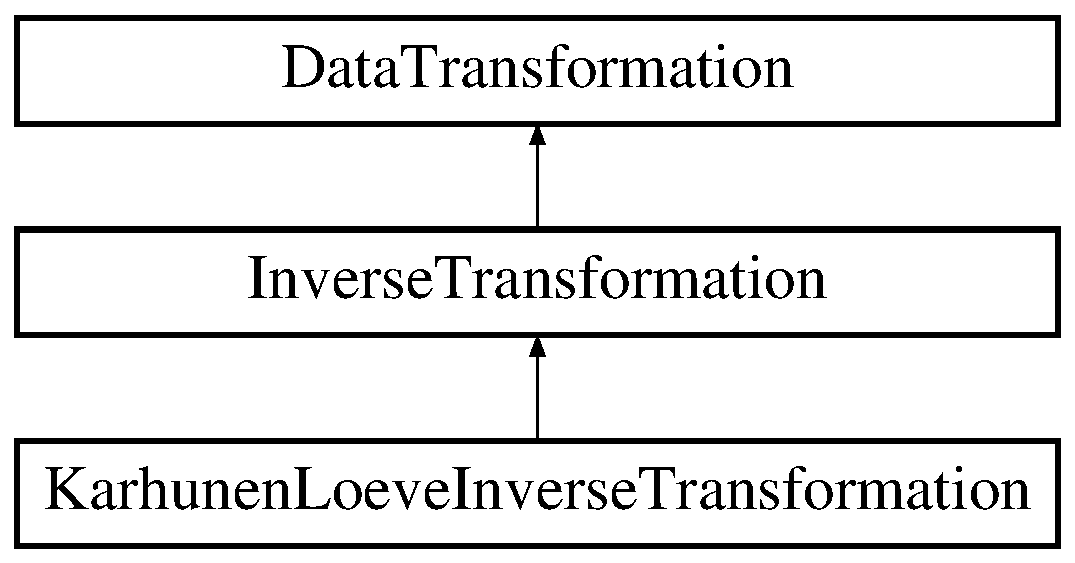
\includegraphics[height=3.000000cm]{classPecos_1_1KarhunenLoeveInverseTransformation}
\end{center}
\end{figure}
\subsection*{Public Member Functions}
\begin{DoxyCompactItemize}
\item 
\hyperlink{classPecos_1_1KarhunenLoeveInverseTransformation_a69c8749d0456df8ddcf8fd460718199b}{Karhunen\+Loeve\+Inverse\+Transformation} ()\label{classPecos_1_1KarhunenLoeveInverseTransformation_a69c8749d0456df8ddcf8fd460718199b}

\begin{DoxyCompactList}\small\item\em constructor \end{DoxyCompactList}\item 
\hyperlink{classPecos_1_1KarhunenLoeveInverseTransformation_ad52d3889f7a6cee422a43da4102fc1a9}{$\sim$\+Karhunen\+Loeve\+Inverse\+Transformation} ()\label{classPecos_1_1KarhunenLoeveInverseTransformation_ad52d3889f7a6cee422a43da4102fc1a9}

\begin{DoxyCompactList}\small\item\em destructor \end{DoxyCompactList}\end{DoxyCompactItemize}
\subsection*{Additional Inherited Members}


\subsection{Detailed Description}
Class for KL data transformation. 

The \hyperlink{classPecos_1_1KarhunenLoeveInverseTransformation}{Karhunen\+Loeve\+Inverse\+Transformation} employs an KL decomposition to map from the frequency domain to the time domain. 

The documentation for this class was generated from the following file\+:\begin{DoxyCompactItemize}
\item 
Karhunen\+Loeve\+Inverse\+Transformation.\+hpp\end{DoxyCompactItemize}

\section{Krawtchouk\+Orthog\+Polynomial Class Reference}
\label{classPecos_1_1KrawtchoukOrthogPolynomial}\index{Krawtchouk\+Orthog\+Polynomial@{Krawtchouk\+Orthog\+Polynomial}}


Derived orthogonal polynomial class for Krawtchouk polynomials.  


Inheritance diagram for Krawtchouk\+Orthog\+Polynomial\+:\begin{figure}[H]
\begin{center}
\leavevmode
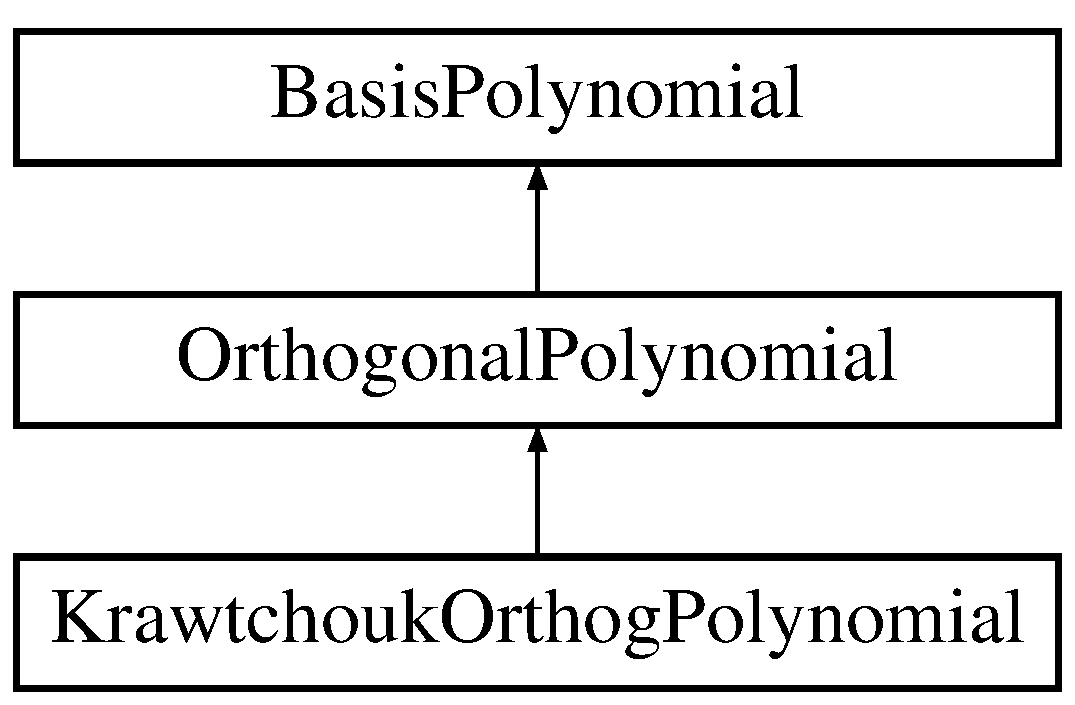
\includegraphics[height=3.000000cm]{classPecos_1_1KrawtchoukOrthogPolynomial}
\end{center}
\end{figure}
\subsection*{Public Member Functions}
\begin{DoxyCompactItemize}
\item 
\hyperlink{classPecos_1_1KrawtchoukOrthogPolynomial_a0bc810e2d27ecfffcbb0f7715c09a772}{Krawtchouk\+Orthog\+Polynomial} ()\label{classPecos_1_1KrawtchoukOrthogPolynomial_a0bc810e2d27ecfffcbb0f7715c09a772}

\begin{DoxyCompactList}\small\item\em default constructor \end{DoxyCompactList}\item 
\hyperlink{classPecos_1_1KrawtchoukOrthogPolynomial_a367830b19e0c13779300ca95a94cbf1f}{$\sim$\+Krawtchouk\+Orthog\+Polynomial} ()\label{classPecos_1_1KrawtchoukOrthogPolynomial_a367830b19e0c13779300ca95a94cbf1f}

\begin{DoxyCompactList}\small\item\em destructor \end{DoxyCompactList}\end{DoxyCompactItemize}
\subsection*{Protected Member Functions}
\begin{DoxyCompactItemize}
\item 
Real \hyperlink{classPecos_1_1KrawtchoukOrthogPolynomial_a8792a858ac05a2158880e876f9da2019}{type1\+\_\+value} (Real x, unsigned short order)
\begin{DoxyCompactList}\small\item\em retrieve the value of the n\+\_\+th type 1 polynomial for a given parameter x using traditional characteristic polynomial formulation \end{DoxyCompactList}\item 
Real \hyperlink{classPecos_1_1KrawtchoukOrthogPolynomial_a997bdeddf670667c476513fcacc779ca}{alpha\+\_\+polynomial} () const \label{classPecos_1_1KrawtchoukOrthogPolynomial_a997bdeddf670667c476513fcacc779ca}

\begin{DoxyCompactList}\small\item\em return alpha\+Poly \end{DoxyCompactList}\item 
Real \hyperlink{classPecos_1_1KrawtchoukOrthogPolynomial_a22bfc4209dec76716ef51648e945469a}{beta\+\_\+polynomial} () const \label{classPecos_1_1KrawtchoukOrthogPolynomial_a22bfc4209dec76716ef51648e945469a}

\begin{DoxyCompactList}\small\item\em return beta\+Poly \end{DoxyCompactList}\item 
void \hyperlink{classPecos_1_1KrawtchoukOrthogPolynomial_aeeb4ce11a8d413209be1ec08eced8728}{alpha\+\_\+stat} (Real alpha)\label{classPecos_1_1KrawtchoukOrthogPolynomial_aeeb4ce11a8d413209be1ec08eced8728}

\begin{DoxyCompactList}\small\item\em set alpha\+Stat (probability per trial) \end{DoxyCompactList}\item 
void \hyperlink{classPecos_1_1KrawtchoukOrthogPolynomial_a7f9584e538ee1574bd4d8d1afb622ed6}{beta\+\_\+stat} (Real beta)\label{classPecos_1_1KrawtchoukOrthogPolynomial_a7f9584e538ee1574bd4d8d1afb622ed6}

\begin{DoxyCompactList}\small\item\em set beta\+Stat (num\+\_\+trials) \end{DoxyCompactList}\end{DoxyCompactItemize}
\subsection*{Private Attributes}
\begin{DoxyCompactItemize}
\item 
Real \hyperlink{classPecos_1_1KrawtchoukOrthogPolynomial_a11666846719189915a02ac6f1f96e393}{alpha\+Poly}\label{classPecos_1_1KrawtchoukOrthogPolynomial_a11666846719189915a02ac6f1f96e393}

\begin{DoxyCompactList}\small\item\em the probability of a \char`\"{}success\char`\"{} for each experiment \end{DoxyCompactList}\item 
short \hyperlink{classPecos_1_1KrawtchoukOrthogPolynomial_af8a06d3cd3f6737b5a9bbc460e4c0d83}{beta\+Poly}\label{classPecos_1_1KrawtchoukOrthogPolynomial_af8a06d3cd3f6737b5a9bbc460e4c0d83}

\begin{DoxyCompactList}\small\item\em the number of discrete points on which to base the polynomial \end{DoxyCompactList}\end{DoxyCompactItemize}
\subsection*{Additional Inherited Members}


\subsection{Detailed Description}
Derived orthogonal polynomial class for Krawtchouk polynomials. 

The \hyperlink{classPecos_1_1KrawtchoukOrthogPolynomial}{Krawtchouk\+Orthog\+Polynomial} class evaluates a univariate Krawtchouk polynomial K$^\wedge$(p,N)\+\_\+n of a particular order. These polynomials are orthogonal with respect to the weight function (N choose k)$\ast$p$^\wedge$k$\ast$(1-\/p)$^\wedge$(n-\/k). This corresponds to the binomial probability mass function, which is the probability of k successes from N trials. See appendix in Xiu \& Karniadakis, Siam J. Sci. Comp., v24, n2, pp. 619-\/644, 2002 for more details. 

\subsection{Member Function Documentation}
\index{Pecos\+::\+Krawtchouk\+Orthog\+Polynomial@{Pecos\+::\+Krawtchouk\+Orthog\+Polynomial}!type1\+\_\+value@{type1\+\_\+value}}
\index{type1\+\_\+value@{type1\+\_\+value}!Pecos\+::\+Krawtchouk\+Orthog\+Polynomial@{Pecos\+::\+Krawtchouk\+Orthog\+Polynomial}}
\subsubsection[{\texorpdfstring{type1\+\_\+value(\+Real x, unsigned short order)}{type1_value(Real x, unsigned short order)}}]{\setlength{\rightskip}{0pt plus 5cm}Real type1\+\_\+value (
\begin{DoxyParamCaption}
\item[{Real}]{x, }
\item[{unsigned short}]{n}
\end{DoxyParamCaption}
)\hspace{0.3cm}{\ttfamily [protected]}, {\ttfamily [virtual]}}\label{classPecos_1_1KrawtchoukOrthogPolynomial_a8792a858ac05a2158880e876f9da2019}


retrieve the value of the n\+\_\+th type 1 polynomial for a given parameter x using traditional characteristic polynomial formulation 

For orthogonal polynomials, n specifies the order of the polynomial, whereas for interpolation polynomials, it identifies the interpolant for the n-\/th point. 

Reimplemented from \hyperlink{classPecos_1_1BasisPolynomial_a1fab871e99cec3a1933a2b1e9ed8a625}{Basis\+Polynomial}.



References Krawtchouk\+Orthog\+Polynomial\+::alpha\+Poly, and Krawtchouk\+Orthog\+Polynomial\+::beta\+Poly.



The documentation for this class was generated from the following files\+:\begin{DoxyCompactItemize}
\item 
Krawtchouk\+Orthog\+Polynomial.\+hpp\item 
Krawtchouk\+Orthog\+Polynomial.\+cpp\end{DoxyCompactItemize}

\section{Lagrange\+Interp\+Polynomial Class Reference}
\label{classPecos_1_1LagrangeInterpPolynomial}\index{Lagrange\+Interp\+Polynomial@{Lagrange\+Interp\+Polynomial}}


Derived basis polynomial class for 1-\/D Lagrange interpolation polynomials.  


Inheritance diagram for Lagrange\+Interp\+Polynomial\+:\begin{figure}[H]
\begin{center}
\leavevmode
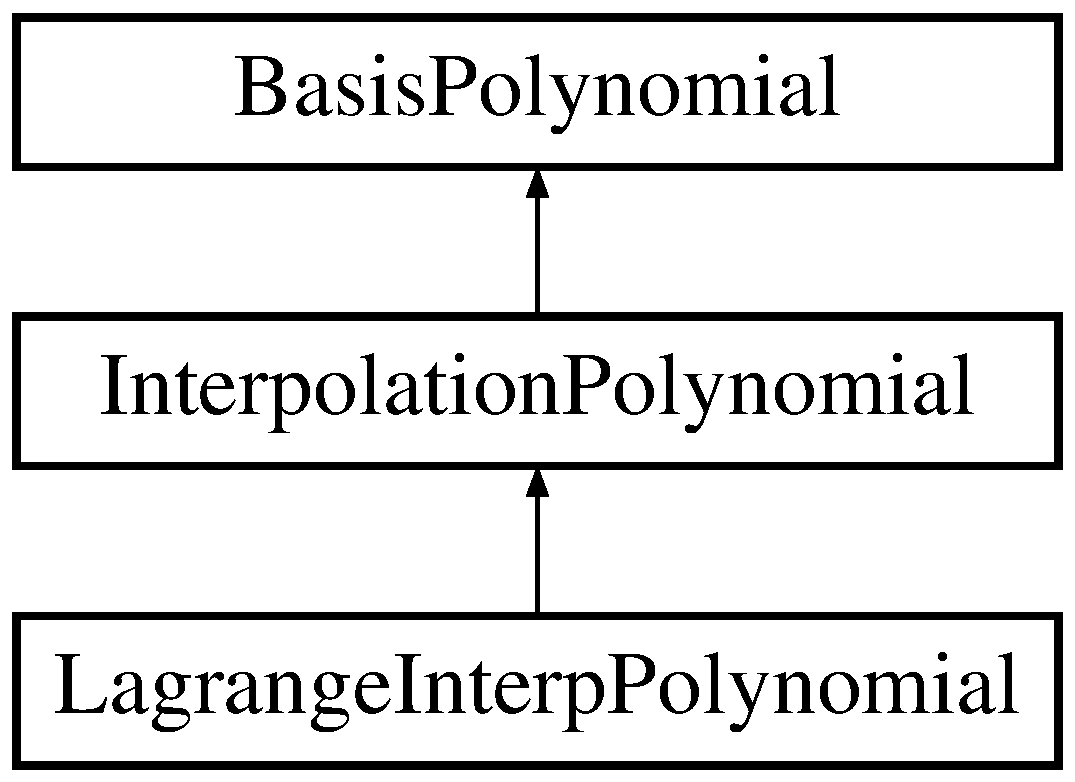
\includegraphics[height=3.000000cm]{classPecos_1_1LagrangeInterpPolynomial}
\end{center}
\end{figure}
\subsection*{Public Member Functions}
\begin{DoxyCompactItemize}
\item 
\hyperlink{classPecos_1_1LagrangeInterpPolynomial_aeb93b2977cfd4d359ecb67c64e2e6800}{Lagrange\+Interp\+Polynomial} ()\label{classPecos_1_1LagrangeInterpPolynomial_aeb93b2977cfd4d359ecb67c64e2e6800}

\begin{DoxyCompactList}\small\item\em default constructor \end{DoxyCompactList}\item 
\hyperlink{classPecos_1_1LagrangeInterpPolynomial_ad045b5254012df8ad6fb5dc8087d6b4c}{Lagrange\+Interp\+Polynomial} (const Real\+Array \&interp\+\_\+pts)\label{classPecos_1_1LagrangeInterpPolynomial_ad045b5254012df8ad6fb5dc8087d6b4c}

\begin{DoxyCompactList}\small\item\em standard constructor \end{DoxyCompactList}\item 
\hyperlink{classPecos_1_1LagrangeInterpPolynomial_a0409bc4b474c957cca221c01b72e1f73}{$\sim$\+Lagrange\+Interp\+Polynomial} ()\label{classPecos_1_1LagrangeInterpPolynomial_a0409bc4b474c957cca221c01b72e1f73}

\begin{DoxyCompactList}\small\item\em destructor \end{DoxyCompactList}\item 
Real \hyperlink{classPecos_1_1LagrangeInterpPolynomial_a2b603ac91089253b885e55fde37cd9c3}{type1\+\_\+value} (unsigned short i)
\begin{DoxyCompactList}\small\item\em retrieve the value of the i\+\_\+th Lagrange polynomial for a given parameter x using barycentric formulation \end{DoxyCompactList}\item 
Real \hyperlink{classPecos_1_1LagrangeInterpPolynomial_abb79c6ea3bd58a7ca9c4b3bfdd85be9c}{type1\+\_\+value} (Real x, unsigned short i)
\begin{DoxyCompactList}\small\item\em retrieve the value of the i\+\_\+th Lagrange polynomial for a given parameter x using traditional characteristic polynomial formulation \end{DoxyCompactList}\item 
Real \hyperlink{classPecos_1_1LagrangeInterpPolynomial_adc62caa2483812a460fa3bd6d5dd79df}{type1\+\_\+gradient} (unsigned short i)
\begin{DoxyCompactList}\small\item\em retrieve the gradient of the i\+\_\+th Lagrange polynomial for a given parameter x using barycentric formulation \end{DoxyCompactList}\item 
Real \hyperlink{classPecos_1_1LagrangeInterpPolynomial_a005465761c081a210eef9879ec5686f8}{type1\+\_\+gradient} (Real x, unsigned short i)
\begin{DoxyCompactList}\small\item\em retrieve the gradient of the i\+\_\+th Lagrange polynomial for a given parameter x using traditional characteristic polynomial formulation \end{DoxyCompactList}\item 
void \hyperlink{classPecos_1_1LagrangeInterpPolynomial_a676f72cadd45161151de088ca488af8a}{set\+\_\+new\+\_\+point} (Real x, short request\+\_\+order)
\item 
void \hyperlink{classPecos_1_1LagrangeInterpPolynomial_ac7d2c87832f8eb608a7d9b9d18013ead}{set\+\_\+new\+\_\+point} (Real x, short request\+\_\+order, const U\+Short\+Array \&delta\+\_\+key)
\item 
size\+\_\+t \hyperlink{classPecos_1_1LagrangeInterpPolynomial_aed1b9a98e9f80287b21581e7278aa253}{exact\+\_\+index} () const \label{classPecos_1_1LagrangeInterpPolynomial_aed1b9a98e9f80287b21581e7278aa253}

\begin{DoxyCompactList}\small\item\em returns the index of a collocation point that is an exact match with the point to be interpolated (from \hyperlink{classPecos_1_1LagrangeInterpPolynomial_a676f72cadd45161151de088ca488af8a}{set\+\_\+new\+\_\+point()}) if detected (\+\_\+\+N\+P\+OS if not) \end{DoxyCompactList}\item 
size\+\_\+t \hyperlink{classPecos_1_1LagrangeInterpPolynomial_a90937bbedd0d5c002f5015cf3847cbaf}{exact\+\_\+delta\+\_\+index} () const \label{classPecos_1_1LagrangeInterpPolynomial_a90937bbedd0d5c002f5015cf3847cbaf}

\begin{DoxyCompactList}\small\item\em returns the index of a hierarchical increment to the interpolation points that is an exact match with the point to be interpolated (from \hyperlink{classPecos_1_1LagrangeInterpPolynomial_a676f72cadd45161151de088ca488af8a}{set\+\_\+new\+\_\+point()}) if detected (\+\_\+\+N\+P\+OS if not) \end{DoxyCompactList}\item 
const Real\+Vector \& \hyperlink{classPecos_1_1LagrangeInterpPolynomial_ab95f72f936b15b2f4cecde96d34d798c}{barycentric\+\_\+value\+\_\+factors} () const \label{classPecos_1_1LagrangeInterpPolynomial_ab95f72f936b15b2f4cecde96d34d798c}

\begin{DoxyCompactList}\small\item\em return the barycentric value factors \end{DoxyCompactList}\item 
const Real\+Vector \& \hyperlink{classPecos_1_1LagrangeInterpPolynomial_a1f77beaf45743dce80d8253b8f7a9394}{barycentric\+\_\+gradient\+\_\+factors} () const \label{classPecos_1_1LagrangeInterpPolynomial_a1f77beaf45743dce80d8253b8f7a9394}

\begin{DoxyCompactList}\small\item\em return the barycentric gradient factors \end{DoxyCompactList}\item 
Real \hyperlink{classPecos_1_1LagrangeInterpPolynomial_a72c4d54d2ef767ab8329f1fb67c7a3fe}{barycentric\+\_\+value\+\_\+factor} (unsigned short i) const \label{classPecos_1_1LagrangeInterpPolynomial_a72c4d54d2ef767ab8329f1fb67c7a3fe}

\begin{DoxyCompactList}\small\item\em return a particular barycentric value factor \end{DoxyCompactList}\item 
Real \hyperlink{classPecos_1_1LagrangeInterpPolynomial_a9cd03b3dfa402dcb120423d116e07d6b}{barycentric\+\_\+gradient\+\_\+factor} (unsigned short i) const \label{classPecos_1_1LagrangeInterpPolynomial_a9cd03b3dfa402dcb120423d116e07d6b}

\begin{DoxyCompactList}\small\item\em return a particular barycentric gradient factor \end{DoxyCompactList}\item 
Real \hyperlink{classPecos_1_1LagrangeInterpPolynomial_ad36b23949c632dd0a6784f82f90050e4}{barycentric\+\_\+value\+\_\+factor\+\_\+sum} () const \label{classPecos_1_1LagrangeInterpPolynomial_ad36b23949c632dd0a6784f82f90050e4}

\begin{DoxyCompactList}\small\item\em return the sum of all barycentric value factors for use in computing the barycentric interpolant denominator \end{DoxyCompactList}\item 
Real \hyperlink{classPecos_1_1LagrangeInterpPolynomial_ae0b1d51779230f3ce9fe3d7c4fc14198}{barycentric\+\_\+difference\+\_\+product} () const \label{classPecos_1_1LagrangeInterpPolynomial_ae0b1d51779230f3ce9fe3d7c4fc14198}

\begin{DoxyCompactList}\small\item\em return the product of all differences between the interpolation points and a current point \end{DoxyCompactList}\end{DoxyCompactItemize}
\subsection*{Protected Member Functions}
\begin{DoxyCompactItemize}
\item 
void \hyperlink{classPecos_1_1LagrangeInterpPolynomial_a9a5fd3dc945d15c8423dc66dcd137b4f}{precompute\+\_\+data} ()
\end{DoxyCompactItemize}
\subsection*{Private Member Functions}
\begin{DoxyCompactItemize}
\item 
void \hyperlink{classPecos_1_1LagrangeInterpPolynomial_aafa5adb96d26d33ef0f61b390d819f66}{init\+\_\+new\+\_\+point} (Real x, short request\+\_\+order, short \&compute\+\_\+order)
\begin{DoxyCompactList}\small\item\em define compute order from request order and new\+Point match \end{DoxyCompactList}\item 
void \hyperlink{classPecos_1_1LagrangeInterpPolynomial_a2a866d84c0640d43946fcde7b0cdd8d6}{allocate\+\_\+factors} (short compute\+\_\+order)
\begin{DoxyCompactList}\small\item\em based on compute order, size barycentric value/gradient factors \end{DoxyCompactList}\end{DoxyCompactItemize}
\subsection*{Private Attributes}
\begin{DoxyCompactItemize}
\item 
Real\+Vector \hyperlink{classPecos_1_1LagrangeInterpPolynomial_ad03ebcd5b1f04eafbe1a63a0f0531323}{bc\+Weights}\label{classPecos_1_1LagrangeInterpPolynomial_ad03ebcd5b1f04eafbe1a63a0f0531323}

\begin{DoxyCompactList}\small\item\em set of denominator products calculated from interp\+Pts in \hyperlink{classPecos_1_1LagrangeInterpPolynomial_a9a5fd3dc945d15c8423dc66dcd137b4f}{precompute\+\_\+data()}; in barycentric formulations, these are the weights \end{DoxyCompactList}\item 
Real \hyperlink{classPecos_1_1LagrangeInterpPolynomial_a313026836e25a5343e39c3d85028ad65}{new\+Point}\label{classPecos_1_1LagrangeInterpPolynomial_a313026836e25a5343e39c3d85028ad65}

\begin{DoxyCompactList}\small\item\em the parameter value for evaluation of the interpolant \end{DoxyCompactList}\item 
short \hyperlink{classPecos_1_1LagrangeInterpPolynomial_a26ebb456478d76c18ce529af2999ada3}{new\+Pt\+Order}\label{classPecos_1_1LagrangeInterpPolynomial_a26ebb456478d76c18ce529af2999ada3}

\begin{DoxyCompactList}\small\item\em order of data that has been precomputed at new\+Point \end{DoxyCompactList}\item 
size\+\_\+t \hyperlink{classPecos_1_1LagrangeInterpPolynomial_a9420cf614b90798b9423727ff03d4731}{exact\+Index}\label{classPecos_1_1LagrangeInterpPolynomial_a9420cf614b90798b9423727ff03d4731}

\begin{DoxyCompactList}\small\item\em index of interpolation point that exactly matches the interpolated value x \end{DoxyCompactList}\item 
size\+\_\+t \hyperlink{classPecos_1_1LagrangeInterpPolynomial_a041eca6801cc6ba2230113995a3d5ac0}{exact\+Delta\+Index}\label{classPecos_1_1LagrangeInterpPolynomial_a041eca6801cc6ba2230113995a3d5ac0}

\begin{DoxyCompactList}\small\item\em index within a hierarchical increment to the interpolation points that exactly matches the interpolated value x \end{DoxyCompactList}\item 
Real \hyperlink{classPecos_1_1LagrangeInterpPolynomial_a0782385d3528cb761abfcc6ea2b3fd5a}{diff\+Product}\label{classPecos_1_1LagrangeInterpPolynomial_a0782385d3528cb761abfcc6ea2b3fd5a}

\begin{DoxyCompactList}\small\item\em product of point differences (x-\/x\+\_\+j) for a particular new\+Point x and interp\+Pts x\+\_\+j \end{DoxyCompactList}\item 
Real\+Vector \hyperlink{classPecos_1_1LagrangeInterpPolynomial_a13d3692709e894353a15de77679689c5}{bc\+Value\+Factors}\label{classPecos_1_1LagrangeInterpPolynomial_a13d3692709e894353a15de77679689c5}

\begin{DoxyCompactList}\small\item\em terms bc\+Weights\mbox{[}j\mbox{]}/(x-\/x\mbox{[}j\mbox{]}) from barycentric formulation \end{DoxyCompactList}\item 
Real \hyperlink{classPecos_1_1LagrangeInterpPolynomial_afa0ec5fd637f41c0510e9114da41d68d}{bc\+Value\+Factor\+Sum}\label{classPecos_1_1LagrangeInterpPolynomial_afa0ec5fd637f41c0510e9114da41d68d}

\begin{DoxyCompactList}\small\item\em sum of bc\+Value\+Factors used for evaluating barycentric interpolant denominator term \end{DoxyCompactList}\item 
Real\+Vector \hyperlink{classPecos_1_1LagrangeInterpPolynomial_a4e3c6bbd363dee4bef97ea9621d54b75}{bc\+Grad\+Factors}\label{classPecos_1_1LagrangeInterpPolynomial_a4e3c6bbd363dee4bef97ea9621d54b75}

\begin{DoxyCompactList}\small\item\em terms for gradients of barycentric interpolants \end{DoxyCompactList}\end{DoxyCompactItemize}
\subsection*{Additional Inherited Members}


\subsection{Detailed Description}
Derived basis polynomial class for 1-\/D Lagrange interpolation polynomials. 

The \hyperlink{classPecos_1_1LagrangeInterpPolynomial}{Lagrange\+Interp\+Polynomial} class evaluates a univariate Lagrange interpolation polynomial. The order of the polynomial is dictated by the number of interpolation points (order = N\+\_\+p -\/ 1). It enables multidimensional interpolants within \hyperlink{classPecos_1_1InterpPolyApproximation}{Interp\+Poly\+Approximation}. This class supports both the traditional characteristic polynomial form of Lagrange interpolation as well as barycentric Lagrange interpolation (the second form from Berrut and Trefethen, 2004). The former is used for actual evaluation of 1D polynomial values (when needed), whereas the latter allows alternative interpolant evaluations with additional precomputation that improve efficiency from O(n$^\wedge$2) evaluations to O(n). 

\subsection{Member Function Documentation}
\index{Pecos\+::\+Lagrange\+Interp\+Polynomial@{Pecos\+::\+Lagrange\+Interp\+Polynomial}!type1\+\_\+value@{type1\+\_\+value}}
\index{type1\+\_\+value@{type1\+\_\+value}!Pecos\+::\+Lagrange\+Interp\+Polynomial@{Pecos\+::\+Lagrange\+Interp\+Polynomial}}
\subsubsection[{\texorpdfstring{type1\+\_\+value(unsigned short i)}{type1_value(unsigned short i)}}]{\setlength{\rightskip}{0pt plus 5cm}Real type1\+\_\+value (
\begin{DoxyParamCaption}
\item[{unsigned short}]{i}
\end{DoxyParamCaption}
)\hspace{0.3cm}{\ttfamily [virtual]}}\label{classPecos_1_1LagrangeInterpPolynomial_a2b603ac91089253b885e55fde37cd9c3}


retrieve the value of the i\+\_\+th Lagrange polynomial for a given parameter x using barycentric formulation 

Compute value of the Lagrange polynomial (1st barycentric form) corresponding to interpolation point i using data from previous call to \hyperlink{classPecos_1_1LagrangeInterpPolynomial_a676f72cadd45161151de088ca488af8a}{set\+\_\+new\+\_\+point()}. 

Reimplemented from \hyperlink{classPecos_1_1BasisPolynomial_a5f87c364dcb43473f02b99b090d99cbb}{Basis\+Polynomial}.



References Lagrange\+Interp\+Polynomial\+::bc\+Value\+Factors, Lagrange\+Interp\+Polynomial\+::diff\+Product, and Lagrange\+Interp\+Polynomial\+::exact\+Index.

\index{Pecos\+::\+Lagrange\+Interp\+Polynomial@{Pecos\+::\+Lagrange\+Interp\+Polynomial}!type1\+\_\+value@{type1\+\_\+value}}
\index{type1\+\_\+value@{type1\+\_\+value}!Pecos\+::\+Lagrange\+Interp\+Polynomial@{Pecos\+::\+Lagrange\+Interp\+Polynomial}}
\subsubsection[{\texorpdfstring{type1\+\_\+value(\+Real x, unsigned short i)}{type1_value(Real x, unsigned short i)}}]{\setlength{\rightskip}{0pt plus 5cm}Real type1\+\_\+value (
\begin{DoxyParamCaption}
\item[{Real}]{x, }
\item[{unsigned short}]{i}
\end{DoxyParamCaption}
)\hspace{0.3cm}{\ttfamily [virtual]}}\label{classPecos_1_1LagrangeInterpPolynomial_abb79c6ea3bd58a7ca9c4b3bfdd85be9c}


retrieve the value of the i\+\_\+th Lagrange polynomial for a given parameter x using traditional characteristic polynomial formulation 

Compute value of the Lagrange polynomial (traditional characteristic polynomial form) corresponding to interpolation point i. 

Reimplemented from \hyperlink{classPecos_1_1BasisPolynomial_a1fab871e99cec3a1933a2b1e9ed8a625}{Basis\+Polynomial}.



References Lagrange\+Interp\+Polynomial\+::bc\+Weights, and Interpolation\+Polynomial\+::interp\+Pts.

\index{Pecos\+::\+Lagrange\+Interp\+Polynomial@{Pecos\+::\+Lagrange\+Interp\+Polynomial}!type1\+\_\+gradient@{type1\+\_\+gradient}}
\index{type1\+\_\+gradient@{type1\+\_\+gradient}!Pecos\+::\+Lagrange\+Interp\+Polynomial@{Pecos\+::\+Lagrange\+Interp\+Polynomial}}
\subsubsection[{\texorpdfstring{type1\+\_\+gradient(unsigned short i)}{type1_gradient(unsigned short i)}}]{\setlength{\rightskip}{0pt plus 5cm}Real type1\+\_\+gradient (
\begin{DoxyParamCaption}
\item[{unsigned short}]{i}
\end{DoxyParamCaption}
)\hspace{0.3cm}{\ttfamily [virtual]}}\label{classPecos_1_1LagrangeInterpPolynomial_adc62caa2483812a460fa3bd6d5dd79df}


retrieve the gradient of the i\+\_\+th Lagrange polynomial for a given parameter x using barycentric formulation 

Compute derivative with respect to x of the Lagrange polynomial (1st barycentric form) corresponding to interpolation point i using data from previous call to \hyperlink{classPecos_1_1LagrangeInterpPolynomial_a676f72cadd45161151de088ca488af8a}{set\+\_\+new\+\_\+point()}. 

Reimplemented from \hyperlink{classPecos_1_1BasisPolynomial_ac88b2920bdede895a618385160254741}{Basis\+Polynomial}.



References Lagrange\+Interp\+Polynomial\+::bc\+Grad\+Factors, Lagrange\+Interp\+Polynomial\+::diff\+Product, and Lagrange\+Interp\+Polynomial\+::exact\+Index.

\index{Pecos\+::\+Lagrange\+Interp\+Polynomial@{Pecos\+::\+Lagrange\+Interp\+Polynomial}!type1\+\_\+gradient@{type1\+\_\+gradient}}
\index{type1\+\_\+gradient@{type1\+\_\+gradient}!Pecos\+::\+Lagrange\+Interp\+Polynomial@{Pecos\+::\+Lagrange\+Interp\+Polynomial}}
\subsubsection[{\texorpdfstring{type1\+\_\+gradient(\+Real x, unsigned short i)}{type1_gradient(Real x, unsigned short i)}}]{\setlength{\rightskip}{0pt plus 5cm}Real type1\+\_\+gradient (
\begin{DoxyParamCaption}
\item[{Real}]{x, }
\item[{unsigned short}]{i}
\end{DoxyParamCaption}
)\hspace{0.3cm}{\ttfamily [virtual]}}\label{classPecos_1_1LagrangeInterpPolynomial_a005465761c081a210eef9879ec5686f8}


retrieve the gradient of the i\+\_\+th Lagrange polynomial for a given parameter x using traditional characteristic polynomial formulation 

Compute derivative with respect to x of the Lagrange polynomial (traditional characteristic polynomial form) corresponding to interpolation point i. 

Reimplemented from \hyperlink{classPecos_1_1BasisPolynomial_a6f69ec84983f551e7e0e4a18b78b4498}{Basis\+Polynomial}.



References Lagrange\+Interp\+Polynomial\+::bc\+Weights, Interpolation\+Polynomial\+::interp\+Pts, and Pecos\+::sum().

\index{Pecos\+::\+Lagrange\+Interp\+Polynomial@{Pecos\+::\+Lagrange\+Interp\+Polynomial}!set\+\_\+new\+\_\+point@{set\+\_\+new\+\_\+point}}
\index{set\+\_\+new\+\_\+point@{set\+\_\+new\+\_\+point}!Pecos\+::\+Lagrange\+Interp\+Polynomial@{Pecos\+::\+Lagrange\+Interp\+Polynomial}}
\subsubsection[{\texorpdfstring{set\+\_\+new\+\_\+point(\+Real x, short request\+\_\+order)}{set_new_point(Real x, short request_order)}}]{\setlength{\rightskip}{0pt plus 5cm}void set\+\_\+new\+\_\+point (
\begin{DoxyParamCaption}
\item[{Real}]{x, }
\item[{short}]{request\+\_\+order}
\end{DoxyParamCaption}
)\hspace{0.3cm}{\ttfamily [virtual]}}\label{classPecos_1_1LagrangeInterpPolynomial_a676f72cadd45161151de088ca488af8a}
Define the bc\+Value\+Factors (and exact\+Index if needed) corresponding to x. 

Reimplemented from \hyperlink{classPecos_1_1BasisPolynomial_afdf46109d433281e37d3de26f4bd1b3d}{Basis\+Polynomial}.



References Lagrange\+Interp\+Polynomial\+::allocate\+\_\+factors(), Lagrange\+Interp\+Polynomial\+::bc\+Grad\+Factors, Lagrange\+Interp\+Polynomial\+::bc\+Value\+Factors, Lagrange\+Interp\+Polynomial\+::bc\+Value\+Factor\+Sum, Lagrange\+Interp\+Polynomial\+::bc\+Weights, Lagrange\+Interp\+Polynomial\+::diff\+Product, Lagrange\+Interp\+Polynomial\+::exact\+Delta\+Index, Lagrange\+Interp\+Polynomial\+::exact\+Index, Lagrange\+Interp\+Polynomial\+::init\+\_\+new\+\_\+point(), Interpolation\+Polynomial\+::interp\+Pts, and Lagrange\+Interp\+Polynomial\+::new\+Point.

\index{Pecos\+::\+Lagrange\+Interp\+Polynomial@{Pecos\+::\+Lagrange\+Interp\+Polynomial}!set\+\_\+new\+\_\+point@{set\+\_\+new\+\_\+point}}
\index{set\+\_\+new\+\_\+point@{set\+\_\+new\+\_\+point}!Pecos\+::\+Lagrange\+Interp\+Polynomial@{Pecos\+::\+Lagrange\+Interp\+Polynomial}}
\subsubsection[{\texorpdfstring{set\+\_\+new\+\_\+point(\+Real x, short request\+\_\+order, const U\+Short\+Array \&delta\+\_\+key)}{set_new_point(Real x, short request_order, const UShortArray &delta_key)}}]{\setlength{\rightskip}{0pt plus 5cm}void set\+\_\+new\+\_\+point (
\begin{DoxyParamCaption}
\item[{Real}]{x, }
\item[{short}]{request\+\_\+order, }
\item[{const U\+Short\+Array \&}]{delta\+\_\+key}
\end{DoxyParamCaption}
)\hspace{0.3cm}{\ttfamily [virtual]}}\label{classPecos_1_1LagrangeInterpPolynomial_ac7d2c87832f8eb608a7d9b9d18013ead}
Define the bc\+Value\+Factors (and exact\+Index if needed) corresponding to x. 

Reimplemented from \hyperlink{classPecos_1_1BasisPolynomial_a01ad737aacfeb1918ffae9b52323336a}{Basis\+Polynomial}.



References Lagrange\+Interp\+Polynomial\+::allocate\+\_\+factors(), Lagrange\+Interp\+Polynomial\+::bc\+Grad\+Factors, Lagrange\+Interp\+Polynomial\+::bc\+Value\+Factors, Lagrange\+Interp\+Polynomial\+::bc\+Value\+Factor\+Sum, Lagrange\+Interp\+Polynomial\+::bc\+Weights, Lagrange\+Interp\+Polynomial\+::diff\+Product, Lagrange\+Interp\+Polynomial\+::exact\+Delta\+Index, Lagrange\+Interp\+Polynomial\+::exact\+Index, Lagrange\+Interp\+Polynomial\+::init\+\_\+new\+\_\+point(), Interpolation\+Polynomial\+::interp\+Pts, and Lagrange\+Interp\+Polynomial\+::new\+Point.

\index{Pecos\+::\+Lagrange\+Interp\+Polynomial@{Pecos\+::\+Lagrange\+Interp\+Polynomial}!precompute\+\_\+data@{precompute\+\_\+data}}
\index{precompute\+\_\+data@{precompute\+\_\+data}!Pecos\+::\+Lagrange\+Interp\+Polynomial@{Pecos\+::\+Lagrange\+Interp\+Polynomial}}
\subsubsection[{\texorpdfstring{precompute\+\_\+data()}{precompute_data()}}]{\setlength{\rightskip}{0pt plus 5cm}void precompute\+\_\+data (
\begin{DoxyParamCaption}
{}
\end{DoxyParamCaption}
)\hspace{0.3cm}{\ttfamily [protected]}, {\ttfamily [virtual]}}\label{classPecos_1_1LagrangeInterpPolynomial_a9a5fd3dc945d15c8423dc66dcd137b4f}
Pre-\/compute denominator products that are only a function of the interpolation points. 

Reimplemented from \hyperlink{classPecos_1_1InterpolationPolynomial_a9a5fd3dc945d15c8423dc66dcd137b4f}{Interpolation\+Polynomial}.



References Lagrange\+Interp\+Polynomial\+::bc\+Weights, Lagrange\+Interp\+Polynomial\+::init\+\_\+new\+\_\+point(), and Interpolation\+Polynomial\+::interp\+Pts.

\index{Pecos\+::\+Lagrange\+Interp\+Polynomial@{Pecos\+::\+Lagrange\+Interp\+Polynomial}!init\+\_\+new\+\_\+point@{init\+\_\+new\+\_\+point}}
\index{init\+\_\+new\+\_\+point@{init\+\_\+new\+\_\+point}!Pecos\+::\+Lagrange\+Interp\+Polynomial@{Pecos\+::\+Lagrange\+Interp\+Polynomial}}
\subsubsection[{\texorpdfstring{init\+\_\+new\+\_\+point(\+Real x, short request\+\_\+order, short \&compute\+\_\+order)}{init_new_point(Real x, short request_order, short &compute_order)}}]{\setlength{\rightskip}{0pt plus 5cm}void init\+\_\+new\+\_\+point (
\begin{DoxyParamCaption}
\item[{Real}]{x, }
\item[{short}]{request\+\_\+order, }
\item[{short \&}]{compute\+\_\+order}
\end{DoxyParamCaption}
)\hspace{0.3cm}{\ttfamily [private]}}\label{classPecos_1_1LagrangeInterpPolynomial_aafa5adb96d26d33ef0f61b390d819f66}


define compute order from request order and new\+Point match 

Shared initialization code. 

References Lagrange\+Interp\+Polynomial\+::exact\+Delta\+Index, Lagrange\+Interp\+Polynomial\+::exact\+Index, Lagrange\+Interp\+Polynomial\+::new\+Point, and Lagrange\+Interp\+Polynomial\+::new\+Pt\+Order.



Referenced by Lagrange\+Interp\+Polynomial\+::precompute\+\_\+data(), and Lagrange\+Interp\+Polynomial\+::set\+\_\+new\+\_\+point().

\index{Pecos\+::\+Lagrange\+Interp\+Polynomial@{Pecos\+::\+Lagrange\+Interp\+Polynomial}!allocate\+\_\+factors@{allocate\+\_\+factors}}
\index{allocate\+\_\+factors@{allocate\+\_\+factors}!Pecos\+::\+Lagrange\+Interp\+Polynomial@{Pecos\+::\+Lagrange\+Interp\+Polynomial}}
\subsubsection[{\texorpdfstring{allocate\+\_\+factors(short compute\+\_\+order)}{allocate_factors(short compute_order)}}]{\setlength{\rightskip}{0pt plus 5cm}void allocate\+\_\+factors (
\begin{DoxyParamCaption}
\item[{short}]{compute\+\_\+order}
\end{DoxyParamCaption}
)\hspace{0.3cm}{\ttfamily [inline]}, {\ttfamily [private]}}\label{classPecos_1_1LagrangeInterpPolynomial_a2a866d84c0640d43946fcde7b0cdd8d6}


based on compute order, size barycentric value/gradient factors 

Shared initialization code. 

References Lagrange\+Interp\+Polynomial\+::bc\+Grad\+Factors, Lagrange\+Interp\+Polynomial\+::bc\+Value\+Factors, Lagrange\+Interp\+Polynomial\+::bc\+Weights, and Interpolation\+Polynomial\+::interp\+Pts.



Referenced by Lagrange\+Interp\+Polynomial\+::set\+\_\+new\+\_\+point().



The documentation for this class was generated from the following files\+:\begin{DoxyCompactItemize}
\item 
Lagrange\+Interp\+Polynomial.\+hpp\item 
Lagrange\+Interp\+Polynomial.\+cpp\end{DoxyCompactItemize}

\section{Laguerre\+Orthog\+Polynomial Class Reference}
\label{classPecos_1_1LaguerreOrthogPolynomial}\index{Laguerre\+Orthog\+Polynomial@{Laguerre\+Orthog\+Polynomial}}


Derived orthogonal polynomial class for Laguerre polynomials.  


Inheritance diagram for Laguerre\+Orthog\+Polynomial\+:\begin{figure}[H]
\begin{center}
\leavevmode
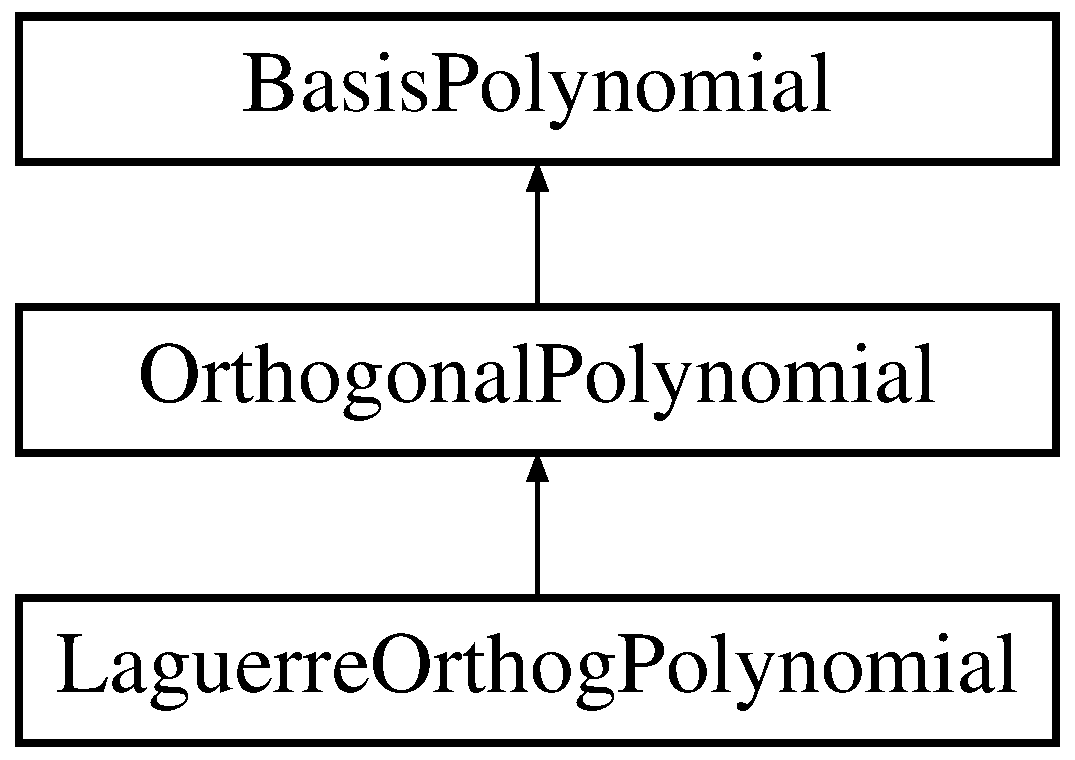
\includegraphics[height=3.000000cm]{classPecos_1_1LaguerreOrthogPolynomial}
\end{center}
\end{figure}
\subsection*{Public Member Functions}
\begin{DoxyCompactItemize}
\item 
\hyperlink{classPecos_1_1LaguerreOrthogPolynomial_ab645e46ecb3df444b3af57a8134fd432}{Laguerre\+Orthog\+Polynomial} ()\label{classPecos_1_1LaguerreOrthogPolynomial_ab645e46ecb3df444b3af57a8134fd432}

\begin{DoxyCompactList}\small\item\em default constructor \end{DoxyCompactList}\item 
\hyperlink{classPecos_1_1LaguerreOrthogPolynomial_a820bc540039324044c8592f173d45dc4}{$\sim$\+Laguerre\+Orthog\+Polynomial} ()\label{classPecos_1_1LaguerreOrthogPolynomial_a820bc540039324044c8592f173d45dc4}

\begin{DoxyCompactList}\small\item\em destructor \end{DoxyCompactList}\end{DoxyCompactItemize}
\subsection*{Protected Member Functions}
\begin{DoxyCompactItemize}
\item 
Real \hyperlink{classPecos_1_1LaguerreOrthogPolynomial_a8792a858ac05a2158880e876f9da2019}{type1\+\_\+value} (Real x, unsigned short order)
\begin{DoxyCompactList}\small\item\em retrieve the value of the n\+\_\+th type 1 polynomial for a given parameter x using traditional characteristic polynomial formulation \end{DoxyCompactList}\item 
Real \hyperlink{classPecos_1_1LaguerreOrthogPolynomial_aac6751aa35bf5fcb42c520a322fc26dc}{type1\+\_\+gradient} (Real x, unsigned short order)
\begin{DoxyCompactList}\small\item\em retrieve the gradient of the n\+\_\+th type 1 polynomial for a given parameter x using traditional characteristic polynomial formulation \end{DoxyCompactList}\item 
Real \hyperlink{classPecos_1_1LaguerreOrthogPolynomial_ae957c8c2e7ea13728bafbad0c9b2996e}{type1\+\_\+hessian} (Real x, unsigned short order)
\begin{DoxyCompactList}\small\item\em retrieve the Hessian of the n\+\_\+th type 1 polynomial for a given parameter x using traditional characteristic polynomial formulation \end{DoxyCompactList}\item 
Real \hyperlink{classPecos_1_1LaguerreOrthogPolynomial_a77c0dbb874af1190d448d01da6efbe4e}{norm\+\_\+squared} (unsigned short order)
\begin{DoxyCompactList}\small\item\em returns the norm-\/squared of the n\+\_\+th order polynomial defined by the inner product $<$Poly\+\_\+n, Poly\+\_\+n$>$ = $\vert$$\vert$\+Poly\+\_\+n$\vert$$\vert$$^\wedge$2 \end{DoxyCompactList}\item 
const Real\+Array \& \hyperlink{classPecos_1_1LaguerreOrthogPolynomial_a10873b28f1284aff4ea214e00c4f86dd}{collocation\+\_\+points} (unsigned short order)
\begin{DoxyCompactList}\small\item\em return collocation points corresponding to orthogonal polynomial order n \end{DoxyCompactList}\item 
const Real\+Array \& \hyperlink{classPecos_1_1LaguerreOrthogPolynomial_aa010321cf47465dca5725fa15ba58bf6}{type1\+\_\+collocation\+\_\+weights} (unsigned short order)
\begin{DoxyCompactList}\small\item\em return the type 1 collocation weights corresponding to a point set of size order \end{DoxyCompactList}\item 
Real \hyperlink{classPecos_1_1LaguerreOrthogPolynomial_a8c1e8d014e82efc5a1c20f973b5bc715}{length\+\_\+scale} () const 
\end{DoxyCompactItemize}
\subsection*{Additional Inherited Members}


\subsection{Detailed Description}
Derived orthogonal polynomial class for Laguerre polynomials. 

The \hyperlink{classPecos_1_1LaguerreOrthogPolynomial}{Laguerre\+Orthog\+Polynomial} class evaluates a univariate Laguerre polynomial of a particular order. These polynomials are orthogonal with respect to the weight function exp(-\/x) when integrated over the support range of \mbox{[}0,+infinity\mbox{]}. This corresponds to the probability density function for the standard exponential distribution. It enables (mixed) multidimensional orthogonal polynomial basis functions within \hyperlink{classPecos_1_1OrthogPolyApproximation}{Orthog\+Poly\+Approximation}. Laguerre polynomials are a special case (alpha = 0) of the generalized Laguerre polynomials (implemented separately) which correspond to the standard gamma distribution. 

\subsection{Member Function Documentation}
\index{Pecos\+::\+Laguerre\+Orthog\+Polynomial@{Pecos\+::\+Laguerre\+Orthog\+Polynomial}!type1\+\_\+value@{type1\+\_\+value}}
\index{type1\+\_\+value@{type1\+\_\+value}!Pecos\+::\+Laguerre\+Orthog\+Polynomial@{Pecos\+::\+Laguerre\+Orthog\+Polynomial}}
\subsubsection[{\texorpdfstring{type1\+\_\+value(\+Real x, unsigned short order)}{type1_value(Real x, unsigned short order)}}]{\setlength{\rightskip}{0pt plus 5cm}Real type1\+\_\+value (
\begin{DoxyParamCaption}
\item[{Real}]{x, }
\item[{unsigned short}]{n}
\end{DoxyParamCaption}
)\hspace{0.3cm}{\ttfamily [protected]}, {\ttfamily [virtual]}}\label{classPecos_1_1LaguerreOrthogPolynomial_a8792a858ac05a2158880e876f9da2019}


retrieve the value of the n\+\_\+th type 1 polynomial for a given parameter x using traditional characteristic polynomial formulation 

For orthogonal polynomials, n specifies the order of the polynomial, whereas for interpolation polynomials, it identifies the interpolant for the n-\/th point. 

Reimplemented from \hyperlink{classPecos_1_1BasisPolynomial_a1fab871e99cec3a1933a2b1e9ed8a625}{Basis\+Polynomial}.



References Laguerre\+Orthog\+Polynomial\+::type1\+\_\+gradient().



Referenced by Laguerre\+Orthog\+Polynomial\+::type1\+\_\+collocation\+\_\+weights(), and Laguerre\+Orthog\+Polynomial\+::type1\+\_\+gradient().

\index{Pecos\+::\+Laguerre\+Orthog\+Polynomial@{Pecos\+::\+Laguerre\+Orthog\+Polynomial}!type1\+\_\+gradient@{type1\+\_\+gradient}}
\index{type1\+\_\+gradient@{type1\+\_\+gradient}!Pecos\+::\+Laguerre\+Orthog\+Polynomial@{Pecos\+::\+Laguerre\+Orthog\+Polynomial}}
\subsubsection[{\texorpdfstring{type1\+\_\+gradient(\+Real x, unsigned short order)}{type1_gradient(Real x, unsigned short order)}}]{\setlength{\rightskip}{0pt plus 5cm}Real type1\+\_\+gradient (
\begin{DoxyParamCaption}
\item[{Real}]{x, }
\item[{unsigned short}]{n}
\end{DoxyParamCaption}
)\hspace{0.3cm}{\ttfamily [protected]}, {\ttfamily [virtual]}}\label{classPecos_1_1LaguerreOrthogPolynomial_aac6751aa35bf5fcb42c520a322fc26dc}


retrieve the gradient of the n\+\_\+th type 1 polynomial for a given parameter x using traditional characteristic polynomial formulation 

For orthogonal polynomials, n specifies the order of the polynomial, whereas for interpolation polynomials, it identifies the interpolant for the n-\/th point. 

Reimplemented from \hyperlink{classPecos_1_1BasisPolynomial_a6f69ec84983f551e7e0e4a18b78b4498}{Basis\+Polynomial}.



References Laguerre\+Orthog\+Polynomial\+::type1\+\_\+value().



Referenced by Laguerre\+Orthog\+Polynomial\+::type1\+\_\+hessian(), and Laguerre\+Orthog\+Polynomial\+::type1\+\_\+value().

\index{Pecos\+::\+Laguerre\+Orthog\+Polynomial@{Pecos\+::\+Laguerre\+Orthog\+Polynomial}!type1\+\_\+hessian@{type1\+\_\+hessian}}
\index{type1\+\_\+hessian@{type1\+\_\+hessian}!Pecos\+::\+Laguerre\+Orthog\+Polynomial@{Pecos\+::\+Laguerre\+Orthog\+Polynomial}}
\subsubsection[{\texorpdfstring{type1\+\_\+hessian(\+Real x, unsigned short order)}{type1_hessian(Real x, unsigned short order)}}]{\setlength{\rightskip}{0pt plus 5cm}Real type1\+\_\+hessian (
\begin{DoxyParamCaption}
\item[{Real}]{x, }
\item[{unsigned short}]{n}
\end{DoxyParamCaption}
)\hspace{0.3cm}{\ttfamily [protected]}, {\ttfamily [virtual]}}\label{classPecos_1_1LaguerreOrthogPolynomial_ae957c8c2e7ea13728bafbad0c9b2996e}


retrieve the Hessian of the n\+\_\+th type 1 polynomial for a given parameter x using traditional characteristic polynomial formulation 

For orthogonal polynomials, n specifies the order of the polynomial, whereas for interpolation polynomials, it identifies the interpolant for the n-\/th point. 

Reimplemented from \hyperlink{classPecos_1_1BasisPolynomial_a07d617dad8572dd606371e6c89ab6c35}{Basis\+Polynomial}.



References Laguerre\+Orthog\+Polynomial\+::type1\+\_\+gradient().

\index{Pecos\+::\+Laguerre\+Orthog\+Polynomial@{Pecos\+::\+Laguerre\+Orthog\+Polynomial}!norm\+\_\+squared@{norm\+\_\+squared}}
\index{norm\+\_\+squared@{norm\+\_\+squared}!Pecos\+::\+Laguerre\+Orthog\+Polynomial@{Pecos\+::\+Laguerre\+Orthog\+Polynomial}}
\subsubsection[{\texorpdfstring{norm\+\_\+squared(unsigned short order)}{norm_squared(unsigned short order)}}]{\setlength{\rightskip}{0pt plus 5cm}Real norm\+\_\+squared (
\begin{DoxyParamCaption}
\item[{unsigned short}]{n}
\end{DoxyParamCaption}
)\hspace{0.3cm}{\ttfamily [protected]}, {\ttfamily [virtual]}}\label{classPecos_1_1LaguerreOrthogPolynomial_a77c0dbb874af1190d448d01da6efbe4e}


returns the norm-\/squared of the n\+\_\+th order polynomial defined by the inner product $<$Poly\+\_\+n, Poly\+\_\+n$>$ = $\vert$$\vert$\+Poly\+\_\+n$\vert$$\vert$$^\wedge$2 

This is defined only for orthogonal polynomials. 

Reimplemented from \hyperlink{classPecos_1_1BasisPolynomial_ab74383be309d74823f2e5e85dad739b2}{Basis\+Polynomial}.



References Laguerre\+Orthog\+Polynomial\+::collocation\+\_\+points().

\index{Pecos\+::\+Laguerre\+Orthog\+Polynomial@{Pecos\+::\+Laguerre\+Orthog\+Polynomial}!collocation\+\_\+points@{collocation\+\_\+points}}
\index{collocation\+\_\+points@{collocation\+\_\+points}!Pecos\+::\+Laguerre\+Orthog\+Polynomial@{Pecos\+::\+Laguerre\+Orthog\+Polynomial}}
\subsubsection[{\texorpdfstring{collocation\+\_\+points(unsigned short order)}{collocation_points(unsigned short order)}}]{\setlength{\rightskip}{0pt plus 5cm}const Real\+Array \& collocation\+\_\+points (
\begin{DoxyParamCaption}
\item[{unsigned short}]{n}
\end{DoxyParamCaption}
)\hspace{0.3cm}{\ttfamily [protected]}, {\ttfamily [virtual]}}\label{classPecos_1_1LaguerreOrthogPolynomial_a10873b28f1284aff4ea214e00c4f86dd}


return collocation points corresponding to orthogonal polynomial order n 

This is defined for orthogonal and piecewise interpolation polynomials. 

Reimplemented from \hyperlink{classPecos_1_1BasisPolynomial_a0f96bd4e27ddc5c44117e7b68744b5a4}{Basis\+Polynomial}.



References Orthogonal\+Polynomial\+::colloc\+Points, Orthogonal\+Polynomial\+::colloc\+Weights, and Laguerre\+Orthog\+Polynomial\+::type1\+\_\+collocation\+\_\+weights().



Referenced by Laguerre\+Orthog\+Polynomial\+::norm\+\_\+squared(), and Laguerre\+Orthog\+Polynomial\+::type1\+\_\+collocation\+\_\+weights().

\index{Pecos\+::\+Laguerre\+Orthog\+Polynomial@{Pecos\+::\+Laguerre\+Orthog\+Polynomial}!type1\+\_\+collocation\+\_\+weights@{type1\+\_\+collocation\+\_\+weights}}
\index{type1\+\_\+collocation\+\_\+weights@{type1\+\_\+collocation\+\_\+weights}!Pecos\+::\+Laguerre\+Orthog\+Polynomial@{Pecos\+::\+Laguerre\+Orthog\+Polynomial}}
\subsubsection[{\texorpdfstring{type1\+\_\+collocation\+\_\+weights(unsigned short order)}{type1_collocation_weights(unsigned short order)}}]{\setlength{\rightskip}{0pt plus 5cm}const Real\+Array \& type1\+\_\+collocation\+\_\+weights (
\begin{DoxyParamCaption}
\item[{unsigned short}]{order}
\end{DoxyParamCaption}
)\hspace{0.3cm}{\ttfamily [protected]}, {\ttfamily [virtual]}}\label{classPecos_1_1LaguerreOrthogPolynomial_aa010321cf47465dca5725fa15ba58bf6}


return the type 1 collocation weights corresponding to a point set of size order 

This is defined for orthogonal and piecewise interpolation polynomials. 

Reimplemented from \hyperlink{classPecos_1_1BasisPolynomial_aa010321cf47465dca5725fa15ba58bf6}{Basis\+Polynomial}.



References Laguerre\+Orthog\+Polynomial\+::collocation\+\_\+points(), Orthogonal\+Polynomial\+::colloc\+Points, Orthogonal\+Polynomial\+::colloc\+Weights, and Laguerre\+Orthog\+Polynomial\+::type1\+\_\+value().



Referenced by Laguerre\+Orthog\+Polynomial\+::collocation\+\_\+points().

\index{Pecos\+::\+Laguerre\+Orthog\+Polynomial@{Pecos\+::\+Laguerre\+Orthog\+Polynomial}!length\+\_\+scale@{length\+\_\+scale}}
\index{length\+\_\+scale@{length\+\_\+scale}!Pecos\+::\+Laguerre\+Orthog\+Polynomial@{Pecos\+::\+Laguerre\+Orthog\+Polynomial}}
\subsubsection[{\texorpdfstring{length\+\_\+scale() const }{length_scale() const }}]{\setlength{\rightskip}{0pt plus 5cm}Real length\+\_\+scale (
\begin{DoxyParamCaption}
{}
\end{DoxyParamCaption}
) const\hspace{0.3cm}{\ttfamily [inline]}, {\ttfamily [protected]}, {\ttfamily [virtual]}}\label{classPecos_1_1LaguerreOrthogPolynomial_a8c1e8d014e82efc5a1c20f973b5bc715}
return mean value 

Reimplemented from \hyperlink{classPecos_1_1BasisPolynomial_a8c1e8d014e82efc5a1c20f973b5bc715}{Basis\+Polynomial}.



The documentation for this class was generated from the following files\+:\begin{DoxyCompactItemize}
\item 
Laguerre\+Orthog\+Polynomial.\+hpp\item 
Laguerre\+Orthog\+Polynomial.\+cpp\end{DoxyCompactItemize}

\section{Legendre\+Orthog\+Polynomial Class Reference}
\label{classPecos_1_1LegendreOrthogPolynomial}\index{Legendre\+Orthog\+Polynomial@{Legendre\+Orthog\+Polynomial}}


Derived orthogonal polynomial class for Legendre polynomials.  


Inheritance diagram for Legendre\+Orthog\+Polynomial\+:\begin{figure}[H]
\begin{center}
\leavevmode
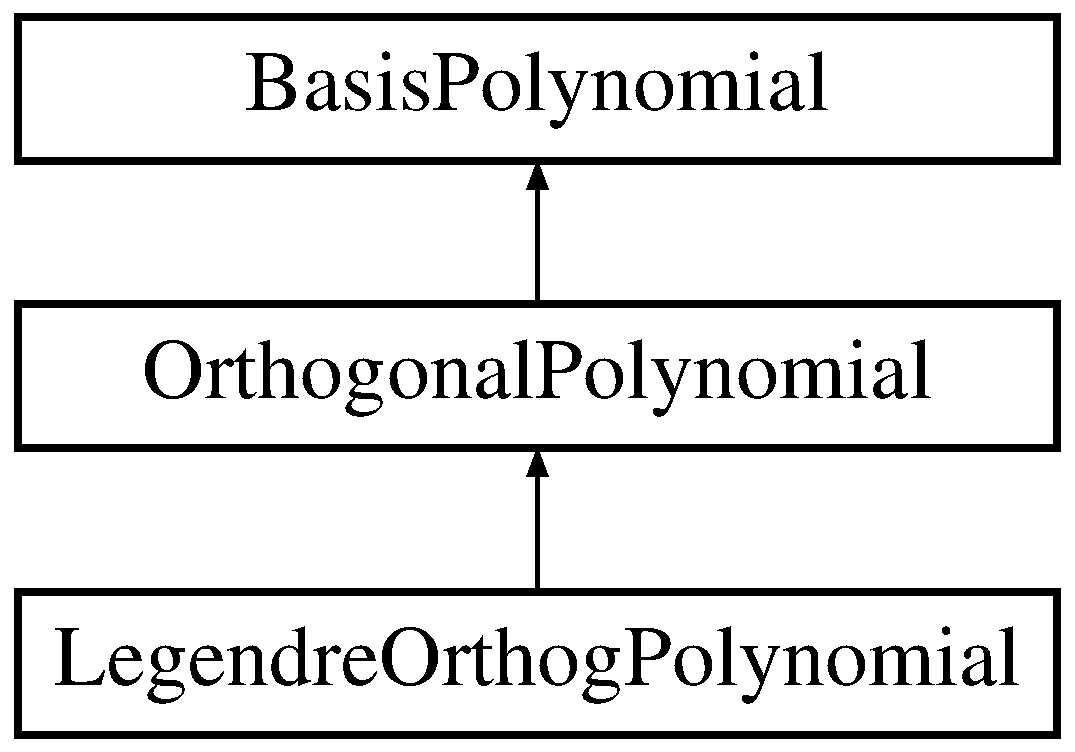
\includegraphics[height=3.000000cm]{classPecos_1_1LegendreOrthogPolynomial}
\end{center}
\end{figure}
\subsection*{Public Member Functions}
\begin{DoxyCompactItemize}
\item 
\hyperlink{classPecos_1_1LegendreOrthogPolynomial_a4ae5004f677ec912e23e278bba014767}{Legendre\+Orthog\+Polynomial} (short colloc\+\_\+rule)\label{classPecos_1_1LegendreOrthogPolynomial_a4ae5004f677ec912e23e278bba014767}

\begin{DoxyCompactList}\small\item\em extended constructor \end{DoxyCompactList}\item 
\hyperlink{classPecos_1_1LegendreOrthogPolynomial_a00e945d1792f3427ef2dccaa9cbfb5af}{Legendre\+Orthog\+Polynomial} ()\label{classPecos_1_1LegendreOrthogPolynomial_a00e945d1792f3427ef2dccaa9cbfb5af}

\begin{DoxyCompactList}\small\item\em default constructor \end{DoxyCompactList}\item 
\hyperlink{classPecos_1_1LegendreOrthogPolynomial_a00265f037d9aaf3cf94a4942157220a5}{$\sim$\+Legendre\+Orthog\+Polynomial} ()\label{classPecos_1_1LegendreOrthogPolynomial_a00265f037d9aaf3cf94a4942157220a5}

\begin{DoxyCompactList}\small\item\em destructor \end{DoxyCompactList}\end{DoxyCompactItemize}
\subsection*{Protected Member Functions}
\begin{DoxyCompactItemize}
\item 
Real \hyperlink{classPecos_1_1LegendreOrthogPolynomial_a8792a858ac05a2158880e876f9da2019}{type1\+\_\+value} (Real x, unsigned short order)
\begin{DoxyCompactList}\small\item\em retrieve the value of the n\+\_\+th type 1 polynomial for a given parameter x using traditional characteristic polynomial formulation \end{DoxyCompactList}\item 
Real \hyperlink{classPecos_1_1LegendreOrthogPolynomial_aac6751aa35bf5fcb42c520a322fc26dc}{type1\+\_\+gradient} (Real x, unsigned short order)
\begin{DoxyCompactList}\small\item\em retrieve the gradient of the n\+\_\+th type 1 polynomial for a given parameter x using traditional characteristic polynomial formulation \end{DoxyCompactList}\item 
Real \hyperlink{classPecos_1_1LegendreOrthogPolynomial_ae957c8c2e7ea13728bafbad0c9b2996e}{type1\+\_\+hessian} (Real x, unsigned short order)
\begin{DoxyCompactList}\small\item\em retrieve the Hessian of the n\+\_\+th type 1 polynomial for a given parameter x using traditional characteristic polynomial formulation \end{DoxyCompactList}\item 
Real \hyperlink{classPecos_1_1LegendreOrthogPolynomial_a77c0dbb874af1190d448d01da6efbe4e}{norm\+\_\+squared} (unsigned short order)
\begin{DoxyCompactList}\small\item\em returns the norm-\/squared of the n\+\_\+th order polynomial defined by the inner product $<$Poly\+\_\+n, Poly\+\_\+n$>$ = $\vert$$\vert$\+Poly\+\_\+n$\vert$$\vert$$^\wedge$2 \end{DoxyCompactList}\item 
const Real\+Array \& \hyperlink{classPecos_1_1LegendreOrthogPolynomial_a10873b28f1284aff4ea214e00c4f86dd}{collocation\+\_\+points} (unsigned short order)
\begin{DoxyCompactList}\small\item\em return collocation points corresponding to orthogonal polynomial order n \end{DoxyCompactList}\item 
const Real\+Array \& \hyperlink{classPecos_1_1LegendreOrthogPolynomial_aa010321cf47465dca5725fa15ba58bf6}{type1\+\_\+collocation\+\_\+weights} (unsigned short order)
\begin{DoxyCompactList}\small\item\em return the type 1 collocation weights corresponding to a point set of size order \end{DoxyCompactList}\item 
Real \hyperlink{classPecos_1_1LegendreOrthogPolynomial_a8c1e8d014e82efc5a1c20f973b5bc715}{length\+\_\+scale} () const 
\end{DoxyCompactItemize}
\subsection*{Additional Inherited Members}


\subsection{Detailed Description}
Derived orthogonal polynomial class for Legendre polynomials. 

The \hyperlink{classPecos_1_1LegendreOrthogPolynomial}{Legendre\+Orthog\+Polynomial} class evaluates a univariate Legendre polynomial of a particular order. These polynomials are orthogonal with respect to the weight function 1 when integrated over the support range of \mbox{[}-\/1,+1\mbox{]}. This corresponds to the probability density function f(x) = 1/(U-\/L) = 1/2 for the uniform distribution for \mbox{[}L,U\mbox{]}=\mbox{[}-\/1,1\mbox{]}. It enables (mixed) multidimensional orthogonal polynomial basis functions within \hyperlink{classPecos_1_1OrthogPolyApproximation}{Orthog\+Poly\+Approximation}. Legendre polynomials are a special case (alpha = beta = 0) of the more general Jacobi polynomials (implemented separately) which correspond to the beta distribution. 

\subsection{Member Function Documentation}
\index{Pecos\+::\+Legendre\+Orthog\+Polynomial@{Pecos\+::\+Legendre\+Orthog\+Polynomial}!type1\+\_\+value@{type1\+\_\+value}}
\index{type1\+\_\+value@{type1\+\_\+value}!Pecos\+::\+Legendre\+Orthog\+Polynomial@{Pecos\+::\+Legendre\+Orthog\+Polynomial}}
\subsubsection[{\texorpdfstring{type1\+\_\+value(\+Real x, unsigned short order)}{type1_value(Real x, unsigned short order)}}]{\setlength{\rightskip}{0pt plus 5cm}Real type1\+\_\+value (
\begin{DoxyParamCaption}
\item[{Real}]{x, }
\item[{unsigned short}]{n}
\end{DoxyParamCaption}
)\hspace{0.3cm}{\ttfamily [protected]}, {\ttfamily [virtual]}}\label{classPecos_1_1LegendreOrthogPolynomial_a8792a858ac05a2158880e876f9da2019}


retrieve the value of the n\+\_\+th type 1 polynomial for a given parameter x using traditional characteristic polynomial formulation 

For orthogonal polynomials, n specifies the order of the polynomial, whereas for interpolation polynomials, it identifies the interpolant for the n-\/th point. 

Reimplemented from \hyperlink{classPecos_1_1BasisPolynomial_a1fab871e99cec3a1933a2b1e9ed8a625}{Basis\+Polynomial}.



Referenced by Legendre\+Orthog\+Polynomial\+::type1\+\_\+collocation\+\_\+weights(), and Legendre\+Orthog\+Polynomial\+::type1\+\_\+gradient().

\index{Pecos\+::\+Legendre\+Orthog\+Polynomial@{Pecos\+::\+Legendre\+Orthog\+Polynomial}!type1\+\_\+gradient@{type1\+\_\+gradient}}
\index{type1\+\_\+gradient@{type1\+\_\+gradient}!Pecos\+::\+Legendre\+Orthog\+Polynomial@{Pecos\+::\+Legendre\+Orthog\+Polynomial}}
\subsubsection[{\texorpdfstring{type1\+\_\+gradient(\+Real x, unsigned short order)}{type1_gradient(Real x, unsigned short order)}}]{\setlength{\rightskip}{0pt plus 5cm}Real type1\+\_\+gradient (
\begin{DoxyParamCaption}
\item[{Real}]{x, }
\item[{unsigned short}]{n}
\end{DoxyParamCaption}
)\hspace{0.3cm}{\ttfamily [protected]}, {\ttfamily [virtual]}}\label{classPecos_1_1LegendreOrthogPolynomial_aac6751aa35bf5fcb42c520a322fc26dc}


retrieve the gradient of the n\+\_\+th type 1 polynomial for a given parameter x using traditional characteristic polynomial formulation 

For orthogonal polynomials, n specifies the order of the polynomial, whereas for interpolation polynomials, it identifies the interpolant for the n-\/th point. 

Reimplemented from \hyperlink{classPecos_1_1BasisPolynomial_a6f69ec84983f551e7e0e4a18b78b4498}{Basis\+Polynomial}.



References Legendre\+Orthog\+Polynomial\+::type1\+\_\+value().



Referenced by Legendre\+Orthog\+Polynomial\+::type1\+\_\+hessian().

\index{Pecos\+::\+Legendre\+Orthog\+Polynomial@{Pecos\+::\+Legendre\+Orthog\+Polynomial}!type1\+\_\+hessian@{type1\+\_\+hessian}}
\index{type1\+\_\+hessian@{type1\+\_\+hessian}!Pecos\+::\+Legendre\+Orthog\+Polynomial@{Pecos\+::\+Legendre\+Orthog\+Polynomial}}
\subsubsection[{\texorpdfstring{type1\+\_\+hessian(\+Real x, unsigned short order)}{type1_hessian(Real x, unsigned short order)}}]{\setlength{\rightskip}{0pt plus 5cm}Real type1\+\_\+hessian (
\begin{DoxyParamCaption}
\item[{Real}]{x, }
\item[{unsigned short}]{n}
\end{DoxyParamCaption}
)\hspace{0.3cm}{\ttfamily [protected]}, {\ttfamily [virtual]}}\label{classPecos_1_1LegendreOrthogPolynomial_ae957c8c2e7ea13728bafbad0c9b2996e}


retrieve the Hessian of the n\+\_\+th type 1 polynomial for a given parameter x using traditional characteristic polynomial formulation 

For orthogonal polynomials, n specifies the order of the polynomial, whereas for interpolation polynomials, it identifies the interpolant for the n-\/th point. 

Reimplemented from \hyperlink{classPecos_1_1BasisPolynomial_a07d617dad8572dd606371e6c89ab6c35}{Basis\+Polynomial}.



References Legendre\+Orthog\+Polynomial\+::type1\+\_\+gradient().

\index{Pecos\+::\+Legendre\+Orthog\+Polynomial@{Pecos\+::\+Legendre\+Orthog\+Polynomial}!norm\+\_\+squared@{norm\+\_\+squared}}
\index{norm\+\_\+squared@{norm\+\_\+squared}!Pecos\+::\+Legendre\+Orthog\+Polynomial@{Pecos\+::\+Legendre\+Orthog\+Polynomial}}
\subsubsection[{\texorpdfstring{norm\+\_\+squared(unsigned short order)}{norm_squared(unsigned short order)}}]{\setlength{\rightskip}{0pt plus 5cm}Real norm\+\_\+squared (
\begin{DoxyParamCaption}
\item[{unsigned short}]{n}
\end{DoxyParamCaption}
)\hspace{0.3cm}{\ttfamily [protected]}, {\ttfamily [virtual]}}\label{classPecos_1_1LegendreOrthogPolynomial_a77c0dbb874af1190d448d01da6efbe4e}


returns the norm-\/squared of the n\+\_\+th order polynomial defined by the inner product $<$Poly\+\_\+n, Poly\+\_\+n$>$ = $\vert$$\vert$\+Poly\+\_\+n$\vert$$\vert$$^\wedge$2 

This is defined only for orthogonal polynomials. 

Reimplemented from \hyperlink{classPecos_1_1BasisPolynomial_ab74383be309d74823f2e5e85dad739b2}{Basis\+Polynomial}.



References Legendre\+Orthog\+Polynomial\+::collocation\+\_\+points().

\index{Pecos\+::\+Legendre\+Orthog\+Polynomial@{Pecos\+::\+Legendre\+Orthog\+Polynomial}!collocation\+\_\+points@{collocation\+\_\+points}}
\index{collocation\+\_\+points@{collocation\+\_\+points}!Pecos\+::\+Legendre\+Orthog\+Polynomial@{Pecos\+::\+Legendre\+Orthog\+Polynomial}}
\subsubsection[{\texorpdfstring{collocation\+\_\+points(unsigned short order)}{collocation_points(unsigned short order)}}]{\setlength{\rightskip}{0pt plus 5cm}const Real\+Array \& collocation\+\_\+points (
\begin{DoxyParamCaption}
\item[{unsigned short}]{n}
\end{DoxyParamCaption}
)\hspace{0.3cm}{\ttfamily [protected]}, {\ttfamily [virtual]}}\label{classPecos_1_1LegendreOrthogPolynomial_a10873b28f1284aff4ea214e00c4f86dd}


return collocation points corresponding to orthogonal polynomial order n 

This is defined for orthogonal and piecewise interpolation polynomials. 

Reimplemented from \hyperlink{classPecos_1_1BasisPolynomial_a0f96bd4e27ddc5c44117e7b68744b5a4}{Basis\+Polynomial}.



References Orthogonal\+Polynomial\+::colloc\+Points, Orthogonal\+Polynomial\+::colloc\+Rule, Orthogonal\+Polynomial\+::colloc\+Weights, Legendre\+Orthog\+Polynomial\+::type1\+\_\+collocation\+\_\+weights(), and Basis\+Polynomial\+::wt\+Factor.



Referenced by Legendre\+Orthog\+Polynomial\+::norm\+\_\+squared(), and Legendre\+Orthog\+Polynomial\+::type1\+\_\+collocation\+\_\+weights().

\index{Pecos\+::\+Legendre\+Orthog\+Polynomial@{Pecos\+::\+Legendre\+Orthog\+Polynomial}!type1\+\_\+collocation\+\_\+weights@{type1\+\_\+collocation\+\_\+weights}}
\index{type1\+\_\+collocation\+\_\+weights@{type1\+\_\+collocation\+\_\+weights}!Pecos\+::\+Legendre\+Orthog\+Polynomial@{Pecos\+::\+Legendre\+Orthog\+Polynomial}}
\subsubsection[{\texorpdfstring{type1\+\_\+collocation\+\_\+weights(unsigned short order)}{type1_collocation_weights(unsigned short order)}}]{\setlength{\rightskip}{0pt plus 5cm}const Real\+Array \& type1\+\_\+collocation\+\_\+weights (
\begin{DoxyParamCaption}
\item[{unsigned short}]{order}
\end{DoxyParamCaption}
)\hspace{0.3cm}{\ttfamily [protected]}, {\ttfamily [virtual]}}\label{classPecos_1_1LegendreOrthogPolynomial_aa010321cf47465dca5725fa15ba58bf6}


return the type 1 collocation weights corresponding to a point set of size order 

This is defined for orthogonal and piecewise interpolation polynomials. 

Reimplemented from \hyperlink{classPecos_1_1BasisPolynomial_aa010321cf47465dca5725fa15ba58bf6}{Basis\+Polynomial}.



References Legendre\+Orthog\+Polynomial\+::collocation\+\_\+points(), Orthogonal\+Polynomial\+::colloc\+Points, Orthogonal\+Polynomial\+::colloc\+Rule, Orthogonal\+Polynomial\+::colloc\+Weights, Legendre\+Orthog\+Polynomial\+::type1\+\_\+value(), and Basis\+Polynomial\+::wt\+Factor.



Referenced by Legendre\+Orthog\+Polynomial\+::collocation\+\_\+points().

\index{Pecos\+::\+Legendre\+Orthog\+Polynomial@{Pecos\+::\+Legendre\+Orthog\+Polynomial}!length\+\_\+scale@{length\+\_\+scale}}
\index{length\+\_\+scale@{length\+\_\+scale}!Pecos\+::\+Legendre\+Orthog\+Polynomial@{Pecos\+::\+Legendre\+Orthog\+Polynomial}}
\subsubsection[{\texorpdfstring{length\+\_\+scale() const }{length_scale() const }}]{\setlength{\rightskip}{0pt plus 5cm}Real length\+\_\+scale (
\begin{DoxyParamCaption}
{}
\end{DoxyParamCaption}
) const\hspace{0.3cm}{\ttfamily [inline]}, {\ttfamily [protected]}, {\ttfamily [virtual]}}\label{classPecos_1_1LegendreOrthogPolynomial_a8c1e8d014e82efc5a1c20f973b5bc715}
\mbox{[}-\/1,1\mbox{]}\+: mean is zero; return std deviation = 2/sqrt(12). 

Reimplemented from \hyperlink{classPecos_1_1BasisPolynomial_a8c1e8d014e82efc5a1c20f973b5bc715}{Basis\+Polynomial}.



The documentation for this class was generated from the following files\+:\begin{DoxyCompactItemize}
\item 
Legendre\+Orthog\+Polynomial.\+hpp\item 
Legendre\+Orthog\+Polynomial.\+cpp\end{DoxyCompactItemize}

\section{L\+H\+S\+Driver Class Reference}
\label{classPecos_1_1LHSDriver}\index{L\+H\+S\+Driver@{L\+H\+S\+Driver}}


Driver class for Latin Hypercube Sampling (L\+HS)  


\subsection*{Public Member Functions}
\begin{DoxyCompactItemize}
\item 
\hyperlink{classPecos_1_1LHSDriver_a63f7ee20058ada4b708b70a7141d6e88}{L\+H\+S\+Driver} ()\label{classPecos_1_1LHSDriver_a63f7ee20058ada4b708b70a7141d6e88}

\begin{DoxyCompactList}\small\item\em default constructor \end{DoxyCompactList}\item 
\hyperlink{classPecos_1_1LHSDriver_a59f03e1cdfb2ddb52b595330656595f6}{L\+H\+S\+Driver} (const String \&sample\+\_\+type, short sample\+\_\+ranks\+\_\+mode=I\+G\+N\+O\+R\+E\+\_\+\+R\+A\+N\+KS, bool reports=true)\label{classPecos_1_1LHSDriver_a59f03e1cdfb2ddb52b595330656595f6}

\begin{DoxyCompactList}\small\item\em constructor \end{DoxyCompactList}\item 
\hyperlink{classPecos_1_1LHSDriver_a2e2bf01d3e26e194124fadb43f00609a}{$\sim$\+L\+H\+S\+Driver} ()\label{classPecos_1_1LHSDriver_a2e2bf01d3e26e194124fadb43f00609a}

\begin{DoxyCompactList}\small\item\em destructor \end{DoxyCompactList}\item 
void \hyperlink{classPecos_1_1LHSDriver_a7a959ceea818c488ad082f91dd3f3d74}{initialize} (const String \&sample\+\_\+type, short sample\+\_\+ranks\+\_\+mode=I\+G\+N\+O\+R\+E\+\_\+\+R\+A\+N\+KS, bool reports=true)\label{classPecos_1_1LHSDriver_a7a959ceea818c488ad082f91dd3f3d74}

\begin{DoxyCompactList}\small\item\em populate data when not passed through ctor \end{DoxyCompactList}\item 
void \hyperlink{classPecos_1_1LHSDriver_ad857540cd2836f32986cf920e68b9de3}{seed} (int seed)\label{classPecos_1_1LHSDriver_ad857540cd2836f32986cf920e68b9de3}

\begin{DoxyCompactList}\small\item\em set random\+Seed \end{DoxyCompactList}\item 
int \hyperlink{classPecos_1_1LHSDriver_ab26add6ea67f675176dae7afae03f03e}{seed} () const \label{classPecos_1_1LHSDriver_ab26add6ea67f675176dae7afae03f03e}

\begin{DoxyCompactList}\small\item\em return random\+Seed \end{DoxyCompactList}\item 
void \hyperlink{classPecos_1_1LHSDriver_a4453b46712e75030a013cf80127fce67}{rng} (String unif\+\_\+gen)\label{classPecos_1_1LHSDriver_a4453b46712e75030a013cf80127fce67}

\begin{DoxyCompactList}\small\item\em set random number generator, passing the name of the uniform generator\+: rnum2 or mt19937 (default). Passed value is superceded by environment variable D\+A\+K\+O\+T\+A\+\_\+\+L\+H\+S\+\_\+\+U\+N\+I\+F\+G\+EN, if present \end{DoxyCompactList}\item 
void \hyperlink{classPecos_1_1LHSDriver_a968dc84c7b328c0fde5435adfbcd4ae4}{advance\+\_\+seed\+\_\+sequence} ()
\begin{DoxyCompactList}\small\item\em reseed using a deterministic sequence \end{DoxyCompactList}\item 
void \hyperlink{classPecos_1_1LHSDriver_a89134ad076d9b362b992f1c4d6beda0b}{generate\+\_\+samples} (const Real\+Vector \&cd\+\_\+l\+\_\+bnds, const Real\+Vector \&cd\+\_\+u\+\_\+bnds, const Int\+Vector \&ddr\+\_\+l\+\_\+bnds, const Int\+Vector \&ddr\+\_\+u\+\_\+bnds, const Int\+Set\+Array \&ddsi\+\_\+values, const String\+Set\+Array \&ddss\+\_\+values, const Real\+Set\+Array \&ddsr\+\_\+values, const Real\+Vector \&cs\+\_\+l\+\_\+bnds, const Real\+Vector \&cs\+\_\+u\+\_\+bnds, const Int\+Vector \&dsr\+\_\+l\+\_\+bnds, const Int\+Vector \&dsr\+\_\+u\+\_\+bnds, const Int\+Set\+Array \&dssi\+\_\+values, const String\+Set\+Array \&dsss\+\_\+values, const Real\+Set\+Array \&dssr\+\_\+values, const \hyperlink{classPecos_1_1AleatoryDistParams}{Aleatory\+Dist\+Params} \&adp, const \hyperlink{classPecos_1_1EpistemicDistParams}{Epistemic\+Dist\+Params} \&edp, int num\+\_\+samples, Real\+Matrix \&samples\+\_\+array, Real\+Matrix \&rank\+\_\+array)
\begin{DoxyCompactList}\small\item\em generates the desired set of parameter samples from within general user-\/specified probabilistic distributions (\hyperlink{classPecos_1_1AleatoryDistParams}{Aleatory\+Dist\+Params} and \hyperlink{classPecos_1_1EpistemicDistParams}{Epistemic\+Dist\+Params} instances augmented with design and state variables) \end{DoxyCompactList}\item 
void \hyperlink{classPecos_1_1LHSDriver_ab6f579d6a8f20974b4de2b41b0256597}{generate\+\_\+samples} (const \hyperlink{classPecos_1_1AleatoryDistParams}{Aleatory\+Dist\+Params} \&adp, const \hyperlink{classPecos_1_1EpistemicDistParams}{Epistemic\+Dist\+Params} \&edp, int num\+\_\+samples, Real\+Matrix \&samples\+\_\+array, bool backfill\+\_\+flag=false)\label{classPecos_1_1LHSDriver_ab6f579d6a8f20974b4de2b41b0256597}

\begin{DoxyCompactList}\small\item\em generates the desired set of parameter samples from within \hyperlink{classPecos_1_1AleatoryDistParams}{Aleatory\+Dist\+Params} and \hyperlink{classPecos_1_1EpistemicDistParams}{Epistemic\+Dist\+Params} specifications \end{DoxyCompactList}\item 
void \hyperlink{classPecos_1_1LHSDriver_ac603c16fc0c6da159f0f2188071fd10f}{generate\+\_\+samples} (const \hyperlink{classPecos_1_1AleatoryDistParams}{Aleatory\+Dist\+Params} \&adp, int num\+\_\+samples, Real\+Matrix \&samples\+\_\+array, bool backfill\+\_\+flag=false)\label{classPecos_1_1LHSDriver_ac603c16fc0c6da159f0f2188071fd10f}

\begin{DoxyCompactList}\small\item\em generates the desired set of parameter samples from within an \hyperlink{classPecos_1_1AleatoryDistParams}{Aleatory\+Dist\+Params} specification \end{DoxyCompactList}\item 
void \hyperlink{classPecos_1_1LHSDriver_a1ea01ac381f57675a33c1330ba48dfa8}{generate\+\_\+samples} (const \hyperlink{classPecos_1_1EpistemicDistParams}{Epistemic\+Dist\+Params} \&edp, int num\+\_\+samples, Real\+Matrix \&samples\+\_\+array, bool backfill\+\_\+flag=false)\label{classPecos_1_1LHSDriver_a1ea01ac381f57675a33c1330ba48dfa8}

\begin{DoxyCompactList}\small\item\em generates the desired set of parameter samples from within a \hyperlink{classPecos_1_1EpistemicDistParams}{Epistemic\+Dist\+Params} specification \end{DoxyCompactList}\item 
void \hyperlink{classPecos_1_1LHSDriver_a3a7e4173b0731e7dcd12828f7cae7732}{generate\+\_\+normal\+\_\+samples} (const Real\+Vector \&n\+\_\+means, const Real\+Vector \&n\+\_\+std\+\_\+devs, const Real\+Vector \&n\+\_\+l\+\_\+bnds, const Real\+Vector \&n\+\_\+u\+\_\+bnds, int num\+\_\+samples, Real\+Sym\+Matrix \&correl\+\_\+matrix, Real\+Matrix \&samples\+\_\+array)\label{classPecos_1_1LHSDriver_a3a7e4173b0731e7dcd12828f7cae7732}

\begin{DoxyCompactList}\small\item\em generates the desired set of parameter samples from within uncorrelated normal distributions \end{DoxyCompactList}\item 
void \hyperlink{classPecos_1_1LHSDriver_ae7a28d8e09d882572dc9d86b1afe5d5f}{generate\+\_\+uniform\+\_\+samples} (const Real\+Vector \&u\+\_\+l\+\_\+bnds, const Real\+Vector \&u\+\_\+u\+\_\+bnds, int num\+\_\+samples, Real\+Matrix \&samples\+\_\+array, bool backfill\+\_\+flag=false)\label{classPecos_1_1LHSDriver_ae7a28d8e09d882572dc9d86b1afe5d5f}

\begin{DoxyCompactList}\small\item\em generates the desired set of parameter samples from within uncorrelated uniform distributions \end{DoxyCompactList}\item 
void \hyperlink{classPecos_1_1LHSDriver_aee047994918369381f1f07bb0635d722}{generate\+\_\+uniform\+\_\+index\+\_\+samples} (const Int\+Vector \&index\+\_\+l\+\_\+bnds, const Int\+Vector \&index\+\_\+u\+\_\+bnds, int num\+\_\+samples, Int\+Matrix \&index\+\_\+samples)\label{classPecos_1_1LHSDriver_aee047994918369381f1f07bb0635d722}

\begin{DoxyCompactList}\small\item\em generates integer index samples from within uncorrelated uniform distributions \end{DoxyCompactList}\item 
void \hyperlink{classPecos_1_1LHSDriver_aef441ba078058c664fd1674840f8a313}{generate\+\_\+unique\+\_\+index\+\_\+samples} (const Int\+Vector \&index\+\_\+l\+\_\+bnds, const Int\+Vector \&index\+\_\+u\+\_\+bnds, int num\+\_\+samples, Int\+Matrix \&sorted\+\_\+samples)\label{classPecos_1_1LHSDriver_aef441ba078058c664fd1674840f8a313}

\begin{DoxyCompactList}\small\item\em generates unique integer index samples from within uncorrelated uniform distributions (more expensive than non-\/unique case) \end{DoxyCompactList}\item 
void \hyperlink{classPecos_1_1LHSDriver_abd371874beed602dd10eab53fd1a70c0}{generate\+\_\+unique\+\_\+samples} (const Real\+Vector \&cd\+\_\+l\+\_\+bnds, const Real\+Vector \&cd\+\_\+u\+\_\+bnds, const Int\+Vector \&ddri\+\_\+l\+\_\+bnds, const Int\+Vector \&ddri\+\_\+u\+\_\+bnds, const Int\+Set\+Array \&ddsi\+\_\+values, const String\+Set\+Array \&ddss\+\_\+values, const Real\+Set\+Array \&ddsr\+\_\+values, const Real\+Vector \&cs\+\_\+l\+\_\+bnds, const Real\+Vector \&cs\+\_\+u\+\_\+bnds, const Int\+Vector \&dsri\+\_\+l\+\_\+bnds, const Int\+Vector \&dsri\+\_\+u\+\_\+bnds, const Int\+Set\+Array \&dssi\+\_\+values, const String\+Set\+Array \&dsss\+\_\+values, const Real\+Set\+Array \&dssr\+\_\+values, const \hyperlink{classPecos_1_1AleatoryDistParams}{Aleatory\+Dist\+Params} \&adp, const \hyperlink{classPecos_1_1EpistemicDistParams}{Epistemic\+Dist\+Params} \&edp, int num\+\_\+samples, Real\+Matrix \&samples, Real\+Matrix \&sample\+\_\+ranks)\label{classPecos_1_1LHSDriver_abd371874beed602dd10eab53fd1a70c0}

\begin{DoxyCompactList}\small\item\em Similar to generate\+\_\+samples but this function ensures that all discrete samples are unique. \end{DoxyCompactList}\end{DoxyCompactItemize}
\subsection*{Private Member Functions}
\begin{DoxyCompactItemize}
\item 
void \hyperlink{classPecos_1_1LHSDriver_a9bdfdc41dd463d47a3a040c37e9ebbe2}{check\+\_\+error} (int err\+\_\+code, const char $\ast$err\+\_\+source) const \label{classPecos_1_1LHSDriver_a9bdfdc41dd463d47a3a040c37e9ebbe2}

\begin{DoxyCompactList}\small\item\em checks the return codes from L\+HS routines and aborts if an error is returned \end{DoxyCompactList}\end{DoxyCompactItemize}
\subsection*{Static Private Member Functions}
\begin{DoxyCompactItemize}
\item 
static void \hyperlink{classPecos_1_1LHSDriver_afa529bd148f75631d3ba0086b65f51e5}{abort\+\_\+if\+\_\+no\+\_\+lhs} ()\label{classPecos_1_1LHSDriver_afa529bd148f75631d3ba0086b65f51e5}

\begin{DoxyCompactList}\small\item\em checks whether L\+HS is enabled in the build and aborts if not \end{DoxyCompactList}\end{DoxyCompactItemize}
\subsection*{Private Attributes}
\begin{DoxyCompactItemize}
\item 
String \hyperlink{classPecos_1_1LHSDriver_abf698fee418ab29591da10a6446c0c18}{sample\+Type}\label{classPecos_1_1LHSDriver_abf698fee418ab29591da10a6446c0c18}

\begin{DoxyCompactList}\small\item\em type of sampling\+: random, lhs, incremental\+\_\+lhs, or incremental\+\_\+random \end{DoxyCompactList}\item 
int \hyperlink{classPecos_1_1LHSDriver_a81ab89411a148610c9749af8e95cd453}{random\+Seed}\label{classPecos_1_1LHSDriver_a81ab89411a148610c9749af8e95cd453}

\begin{DoxyCompactList}\small\item\em the current random number seed \end{DoxyCompactList}\item 
short \hyperlink{classPecos_1_1LHSDriver_ac44aac00b4d7c697a8e5d8f32acccaf2}{sample\+Ranks\+Mode}\label{classPecos_1_1LHSDriver_ac44aac00b4d7c697a8e5d8f32acccaf2}

\begin{DoxyCompactList}\small\item\em mode of sample ranks I/O\+: I\+G\+N\+O\+R\+E\+\_\+\+R\+A\+N\+KS, S\+E\+T\+\_\+\+R\+A\+N\+KS, G\+E\+T\+\_\+\+R\+A\+N\+KS, or S\+E\+T\+\_\+\+G\+E\+T\+\_\+\+R\+A\+N\+KS \end{DoxyCompactList}\item 
bool \hyperlink{classPecos_1_1LHSDriver_a6659689711fd1c7d227a7c8a4e093d12}{report\+Flag}\label{classPecos_1_1LHSDriver_a6659689711fd1c7d227a7c8a4e093d12}

\begin{DoxyCompactList}\small\item\em flag for generating L\+HS report output \end{DoxyCompactList}\item 
short \hyperlink{classPecos_1_1LHSDriver_abc4c4d1b5324bce157150cda69831718}{allow\+Seed\+Advance}\label{classPecos_1_1LHSDriver_abc4c4d1b5324bce157150cda69831718}

\begin{DoxyCompactList}\small\item\em for honoring \hyperlink{classPecos_1_1LHSDriver_a968dc84c7b328c0fde5435adfbcd4ae4}{advance\+\_\+seed\+\_\+sequence()} calls \end{DoxyCompactList}\end{DoxyCompactItemize}


\subsection{Detailed Description}
Driver class for Latin Hypercube Sampling (L\+HS) 

This class provides common code for sampling methods which employ the Latin Hypercube Sampling (L\+HS) package from Sandia Albuquerque\textquotesingle{}s Risk and Reliability organization. 

\subsection{Member Function Documentation}
\index{Pecos\+::\+L\+H\+S\+Driver@{Pecos\+::\+L\+H\+S\+Driver}!advance\+\_\+seed\+\_\+sequence@{advance\+\_\+seed\+\_\+sequence}}
\index{advance\+\_\+seed\+\_\+sequence@{advance\+\_\+seed\+\_\+sequence}!Pecos\+::\+L\+H\+S\+Driver@{Pecos\+::\+L\+H\+S\+Driver}}
\subsubsection[{\texorpdfstring{advance\+\_\+seed\+\_\+sequence()}{advance_seed_sequence()}}]{\setlength{\rightskip}{0pt plus 5cm}void advance\+\_\+seed\+\_\+sequence (
\begin{DoxyParamCaption}
{}
\end{DoxyParamCaption}
)\hspace{0.3cm}{\ttfamily [inline]}}\label{classPecos_1_1LHSDriver_a968dc84c7b328c0fde5435adfbcd4ae4}


reseed using a deterministic sequence 

It would be preferable to call srand() only once and then call rand() for each L\+HS execution (the intended usage model), but possible interaction with other uses of rand() in other contexts is a concern. E.\+g., an srand(clock()) executed elsewhere would ruin the repeatability of the \hyperlink{classPecos_1_1LHSDriver}{L\+H\+S\+Driver} seed sequence. The only way to insure isolation is to reseed each time. Any induced correlation should be inconsequential for the intended use. 

References L\+H\+S\+Driver\+::allow\+Seed\+Advance, L\+H\+S\+Driver\+::generate\+\_\+samples(), L\+H\+S\+Driver\+::random\+Seed, and L\+H\+S\+Driver\+::seed().



Referenced by Fourier\+Inverse\+Transformation\+::compute\+\_\+sample\+\_\+grigoriu(), and Fourier\+Inverse\+Transformation\+::compute\+\_\+sample\+\_\+shinozuka\+\_\+deodatis().

\index{Pecos\+::\+L\+H\+S\+Driver@{Pecos\+::\+L\+H\+S\+Driver}!generate\+\_\+samples@{generate\+\_\+samples}}
\index{generate\+\_\+samples@{generate\+\_\+samples}!Pecos\+::\+L\+H\+S\+Driver@{Pecos\+::\+L\+H\+S\+Driver}}
\subsubsection[{\texorpdfstring{generate\+\_\+samples(const Real\+Vector \&cd\+\_\+l\+\_\+bnds, const Real\+Vector \&cd\+\_\+u\+\_\+bnds, const Int\+Vector \&ddr\+\_\+l\+\_\+bnds, const Int\+Vector \&ddr\+\_\+u\+\_\+bnds, const Int\+Set\+Array \&ddsi\+\_\+values, const String\+Set\+Array \&ddss\+\_\+values, const Real\+Set\+Array \&ddsr\+\_\+values, const Real\+Vector \&cs\+\_\+l\+\_\+bnds, const Real\+Vector \&cs\+\_\+u\+\_\+bnds, const Int\+Vector \&dsr\+\_\+l\+\_\+bnds, const Int\+Vector \&dsr\+\_\+u\+\_\+bnds, const Int\+Set\+Array \&dssi\+\_\+values, const String\+Set\+Array \&dsss\+\_\+values, const Real\+Set\+Array \&dssr\+\_\+values, const Aleatory\+Dist\+Params \&adp, const Epistemic\+Dist\+Params \&edp, int num\+\_\+samples, Real\+Matrix \&samples\+\_\+array, Real\+Matrix \&rank\+\_\+array)}{generate_samples(const RealVector &cd_l_bnds, const RealVector &cd_u_bnds, const IntVector &ddr_l_bnds, const IntVector &ddr_u_bnds, const IntSetArray &ddsi_values, const StringSetArray &ddss_values, const RealSetArray &ddsr_values, const RealVector &cs_l_bnds, const RealVector &cs_u_bnds, const IntVector &dsr_l_bnds, const IntVector &dsr_u_bnds, const IntSetArray &dssi_values, const StringSetArray &dsss_values, const RealSetArray &dssr_values, const AleatoryDistParams &adp, const EpistemicDistParams &edp, int num_samples, RealMatrix &samples_array, RealMatrix &rank_array)}}]{\setlength{\rightskip}{0pt plus 5cm}void generate\+\_\+samples (
\begin{DoxyParamCaption}
\item[{const Real\+Vector \&}]{cd\+\_\+l\+\_\+bnds, }
\item[{const Real\+Vector \&}]{cd\+\_\+u\+\_\+bnds, }
\item[{const Int\+Vector \&}]{ddri\+\_\+l\+\_\+bnds, }
\item[{const Int\+Vector \&}]{ddri\+\_\+u\+\_\+bnds, }
\item[{const Int\+Set\+Array \&}]{ddsi\+\_\+values, }
\item[{const String\+Set\+Array \&}]{ddss\+\_\+values, }
\item[{const Real\+Set\+Array \&}]{ddsr\+\_\+values, }
\item[{const Real\+Vector \&}]{cs\+\_\+l\+\_\+bnds, }
\item[{const Real\+Vector \&}]{cs\+\_\+u\+\_\+bnds, }
\item[{const Int\+Vector \&}]{dsri\+\_\+l\+\_\+bnds, }
\item[{const Int\+Vector \&}]{dsri\+\_\+u\+\_\+bnds, }
\item[{const Int\+Set\+Array \&}]{dssi\+\_\+values, }
\item[{const String\+Set\+Array \&}]{dsss\+\_\+values, }
\item[{const Real\+Set\+Array \&}]{dssr\+\_\+values, }
\item[{const {\bf Aleatory\+Dist\+Params} \&}]{adp, }
\item[{const {\bf Epistemic\+Dist\+Params} \&}]{edp, }
\item[{int}]{num\+\_\+samples, }
\item[{Real\+Matrix \&}]{samples, }
\item[{Real\+Matrix \&}]{sample\+\_\+ranks}
\end{DoxyParamCaption}
)}\label{classPecos_1_1LHSDriver_a89134ad076d9b362b992f1c4d6beda0b}


generates the desired set of parameter samples from within general user-\/specified probabilistic distributions (\hyperlink{classPecos_1_1AleatoryDistParams}{Aleatory\+Dist\+Params} and \hyperlink{classPecos_1_1EpistemicDistParams}{Epistemic\+Dist\+Params} instances augmented with design and state variables) 

While it would be desirable in some cases to carve this function into smaller parts and allow multiple invocations of L\+H\+S\+\_\+\+R\+UN following a single initialization of types and arrays, the L\+HS code does not currently allow this\+: it will return an error if L\+H\+S\+\_\+\+I\+N\+I\+T/\+L\+H\+S\+\_\+\+I\+N\+I\+T\+\_\+\+M\+EM, at least one distribution call (i.\+e., L\+H\+S\+\_\+\+D\+I\+ST, L\+H\+S\+\_\+\+U\+D\+I\+ST or L\+H\+S\+\_\+\+S\+D\+I\+ST), and L\+H\+S\+\_\+\+P\+R\+EP are not called prior to each invocation of L\+H\+S\+\_\+\+R\+UN. Since L\+H\+S\+\_\+\+I\+N\+I\+T/\+L\+H\+S\+\_\+\+I\+N\+I\+T\+\_\+\+M\+EM require input of a seed, the approach to computing multiple distinct sample sets must employ \hyperlink{classPecos_1_1LHSDriver_a968dc84c7b328c0fde5435adfbcd4ae4}{advance\+\_\+seed\+\_\+sequence()} to re-\/seed multiple \hyperlink{classPecos_1_1LHSDriver_a89134ad076d9b362b992f1c4d6beda0b}{generate\+\_\+samples()} calls, rather than continuing an existing random number sequence. 

References Aleatory\+Dist\+Params\+::beta\+\_\+alphas(), Aleatory\+Dist\+Params\+::beta\+\_\+betas(), Aleatory\+Dist\+Params\+::beta\+\_\+lower\+\_\+bounds(), Aleatory\+Dist\+Params\+::beta\+\_\+upper\+\_\+bounds(), Aleatory\+Dist\+Params\+::binomial\+\_\+num\+\_\+trials(), Aleatory\+Dist\+Params\+::binomial\+\_\+probability\+\_\+per\+\_\+trial(), L\+H\+S\+Driver\+::check\+\_\+error(), Epistemic\+Dist\+Params\+::continuous\+\_\+interval\+\_\+basic\+\_\+probabilities(), Epistemic\+Dist\+Params\+::discrete\+\_\+interval\+\_\+basic\+\_\+probabilities(), Epistemic\+Dist\+Params\+::discrete\+\_\+set\+\_\+int\+\_\+values\+\_\+probabilities(), Epistemic\+Dist\+Params\+::discrete\+\_\+set\+\_\+real\+\_\+values\+\_\+probabilities(), Epistemic\+Dist\+Params\+::discrete\+\_\+set\+\_\+string\+\_\+values\+\_\+probabilities(), Aleatory\+Dist\+Params\+::exponential\+\_\+betas(), Aleatory\+Dist\+Params\+::frechet\+\_\+alphas(), Aleatory\+Dist\+Params\+::frechet\+\_\+betas(), Aleatory\+Dist\+Params\+::gamma\+\_\+alphas(), Aleatory\+Dist\+Params\+::gamma\+\_\+betas(), L\+H\+S\+Driver\+::generate\+\_\+unique\+\_\+samples(), Aleatory\+Dist\+Params\+::geometric\+\_\+probability\+\_\+per\+\_\+trial(), Aleatory\+Dist\+Params\+::gumbel\+\_\+alphas(), Aleatory\+Dist\+Params\+::gumbel\+\_\+betas(), Aleatory\+Dist\+Params\+::histogram\+\_\+bin\+\_\+pairs(), Aleatory\+Dist\+Params\+::histogram\+\_\+point\+\_\+int\+\_\+pairs(), Aleatory\+Dist\+Params\+::histogram\+\_\+point\+\_\+real\+\_\+pairs(), Aleatory\+Dist\+Params\+::histogram\+\_\+point\+\_\+string\+\_\+pairs(), Aleatory\+Dist\+Params\+::hypergeometric\+\_\+num\+\_\+drawn(), Aleatory\+Dist\+Params\+::hypergeometric\+\_\+selected\+\_\+population(), Aleatory\+Dist\+Params\+::hypergeometric\+\_\+total\+\_\+population(), Aleatory\+Dist\+Params\+::lognormal\+\_\+error\+\_\+factors(), Aleatory\+Dist\+Params\+::lognormal\+\_\+lambdas(), Aleatory\+Dist\+Params\+::lognormal\+\_\+lower\+\_\+bounds(), Aleatory\+Dist\+Params\+::lognormal\+\_\+means(), Aleatory\+Dist\+Params\+::lognormal\+\_\+std\+\_\+deviations(), Aleatory\+Dist\+Params\+::lognormal\+\_\+upper\+\_\+bounds(), Aleatory\+Dist\+Params\+::lognormal\+\_\+zetas(), Aleatory\+Dist\+Params\+::loguniform\+\_\+lower\+\_\+bounds(), Aleatory\+Dist\+Params\+::loguniform\+\_\+upper\+\_\+bounds(), Aleatory\+Dist\+Params\+::negative\+\_\+binomial\+\_\+num\+\_\+trials(), Aleatory\+Dist\+Params\+::negative\+\_\+binomial\+\_\+probability\+\_\+per\+\_\+trial(), Aleatory\+Dist\+Params\+::normal\+\_\+lower\+\_\+bounds(), Aleatory\+Dist\+Params\+::normal\+\_\+means(), Aleatory\+Dist\+Params\+::normal\+\_\+std\+\_\+deviations(), Aleatory\+Dist\+Params\+::normal\+\_\+upper\+\_\+bounds(), Aleatory\+Dist\+Params\+::poisson\+\_\+lambdas(), L\+H\+S\+Driver\+::random\+Seed, L\+H\+S\+Driver\+::report\+Flag, L\+H\+S\+Driver\+::sample\+Ranks\+Mode, L\+H\+S\+Driver\+::sample\+Type, Aleatory\+Dist\+Params\+::triangular\+\_\+lower\+\_\+bounds(), Aleatory\+Dist\+Params\+::triangular\+\_\+modes(), Aleatory\+Dist\+Params\+::triangular\+\_\+upper\+\_\+bounds(), Aleatory\+Dist\+Params\+::uncertain\+\_\+correlations(), Aleatory\+Dist\+Params\+::uniform\+\_\+lower\+\_\+bounds(), Aleatory\+Dist\+Params\+::uniform\+\_\+upper\+\_\+bounds(), Aleatory\+Dist\+Params\+::weibull\+\_\+alphas(), and Aleatory\+Dist\+Params\+::weibull\+\_\+betas().



Referenced by L\+H\+S\+Driver\+::abort\+\_\+if\+\_\+no\+\_\+lhs(), L\+H\+S\+Driver\+::advance\+\_\+seed\+\_\+sequence(), L\+H\+S\+Driver\+::generate\+\_\+normal\+\_\+samples(), L\+H\+S\+Driver\+::generate\+\_\+samples(), L\+H\+S\+Driver\+::generate\+\_\+uniform\+\_\+index\+\_\+samples(), L\+H\+S\+Driver\+::generate\+\_\+uniform\+\_\+samples(), and L\+H\+S\+Driver\+::generate\+\_\+unique\+\_\+samples().



The documentation for this class was generated from the following files\+:\begin{DoxyCompactItemize}
\item 
L\+H\+S\+Driver.\+hpp\item 
L\+H\+S\+Driver.\+cpp\end{DoxyCompactItemize}

\section{Lightweight\+Sparse\+Grid\+Driver Class Reference}
\label{classPecos_1_1LightweightSparseGridDriver}\index{Lightweight\+Sparse\+Grid\+Driver@{Lightweight\+Sparse\+Grid\+Driver}}


Lighweight sparse grid driver class that generates index sets for N-\/dimensional Smolyak sparse grids.  


Inheritance diagram for Lightweight\+Sparse\+Grid\+Driver\+:\begin{figure}[H]
\begin{center}
\leavevmode
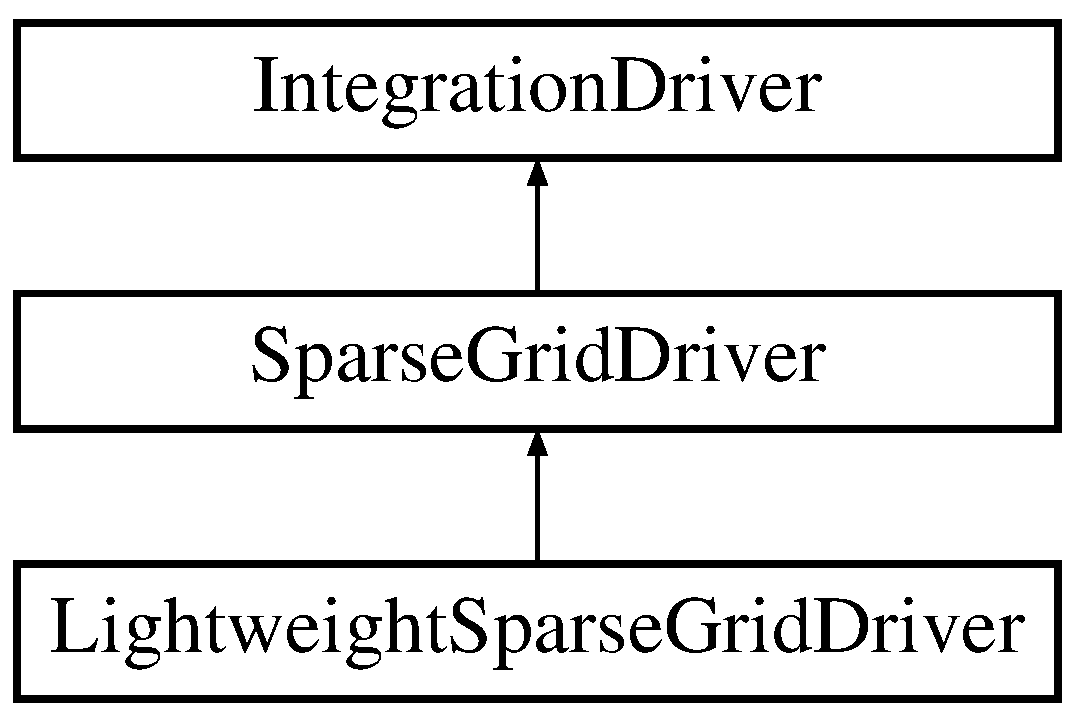
\includegraphics[height=3.000000cm]{classPecos_1_1LightweightSparseGridDriver}
\end{center}
\end{figure}
\subsection*{Public Member Functions}
\begin{DoxyCompactItemize}
\item 
\hyperlink{classPecos_1_1LightweightSparseGridDriver_a258a4f02a1442f1580ae51823b28e7b9}{Lightweight\+Sparse\+Grid\+Driver} ()\label{classPecos_1_1LightweightSparseGridDriver_a258a4f02a1442f1580ae51823b28e7b9}

\begin{DoxyCompactList}\small\item\em default constructor \end{DoxyCompactList}\item 
\hyperlink{classPecos_1_1LightweightSparseGridDriver_aeb28d870b34f91c2e9b935d68466b731}{Lightweight\+Sparse\+Grid\+Driver} (unsigned short ssg\+\_\+level, const Real\+Vector \&dim\+\_\+pref=Real\+Vector(), short \hyperlink{classPecos_1_1SparseGridDriver_a6f9061513ba25c62ee7a49b0d5da42cc}{growth\+\_\+rate}=M\+O\+D\+E\+R\+A\+T\+E\+\_\+\+R\+E\+S\+T\+R\+I\+C\+T\+E\+D\+\_\+\+G\+R\+O\+W\+TH, short refine\+\_\+control=N\+O\+\_\+\+C\+O\+N\+T\+R\+OL)\label{classPecos_1_1LightweightSparseGridDriver_aeb28d870b34f91c2e9b935d68466b731}

\begin{DoxyCompactList}\small\item\em constructor \end{DoxyCompactList}\item 
\hyperlink{classPecos_1_1LightweightSparseGridDriver_a27a8fed45f7f78fdbdbbb2c041de7b4c}{$\sim$\+Lightweight\+Sparse\+Grid\+Driver} ()\label{classPecos_1_1LightweightSparseGridDriver_a27a8fed45f7f78fdbdbbb2c041de7b4c}

\begin{DoxyCompactList}\small\item\em destructor \end{DoxyCompactList}\item 
void \hyperlink{classPecos_1_1LightweightSparseGridDriver_a059e9e1e03a5cd29771d369b76311261}{initialize\+\_\+sets} ()
\begin{DoxyCompactList}\small\item\em initializes old/active/evaluation sets for use within the generalized sparse grid procedure \end{DoxyCompactList}\item 
void \hyperlink{classPecos_1_1LightweightSparseGridDriver_a99c17efb3a8e873b7708652cc1787370}{push\+\_\+trial\+\_\+set} (const U\+Short\+Array \&set)\label{classPecos_1_1LightweightSparseGridDriver_a99c17efb3a8e873b7708652cc1787370}

\begin{DoxyCompactList}\small\item\em update smolyak\+Multi\+Index with a new trial set for use within the generalized sparse grid procedure \end{DoxyCompactList}\item 
void \hyperlink{classPecos_1_1LightweightSparseGridDriver_a92b2604a79028bec35c176aee27e56bb}{pop\+\_\+trial\+\_\+set} ()\label{classPecos_1_1LightweightSparseGridDriver_a92b2604a79028bec35c176aee27e56bb}

\begin{DoxyCompactList}\small\item\em remove the previously pushed trial set from smolyak\+Multi\+Index during the course of the generalized sparse grid procedure \end{DoxyCompactList}\item 
const U\+Short\+Array \& \hyperlink{classPecos_1_1LightweightSparseGridDriver_a5c92e49dbfbcfa5b0d1523ed254b4d76}{trial\+\_\+set} () const \label{classPecos_1_1LightweightSparseGridDriver_a5c92e49dbfbcfa5b0d1523ed254b4d76}

\begin{DoxyCompactList}\small\item\em return the trial index set from \hyperlink{classPecos_1_1LightweightSparseGridDriver_a99c17efb3a8e873b7708652cc1787370}{push\+\_\+trial\+\_\+set()} \end{DoxyCompactList}\item 
void \hyperlink{classPecos_1_1LightweightSparseGridDriver_ae5bcc14a0e7bb726d5280c3dd10e6c98}{print\+\_\+smolyak\+\_\+multi\+\_\+index} () const \label{classPecos_1_1LightweightSparseGridDriver_ae5bcc14a0e7bb726d5280c3dd10e6c98}

\begin{DoxyCompactList}\small\item\em print smolyak\+Multi\+Index \end{DoxyCompactList}\item 
void \hyperlink{classPecos_1_1LightweightSparseGridDriver_ac6105d921fa39880b9ffddaab414bb3f}{initialize\+\_\+grid} (size\+\_\+t num\+\_\+v, unsigned short ssg\+\_\+level)
\begin{DoxyCompactList}\small\item\em initialize a lightweight instance that only generates index sets \end{DoxyCompactList}\item 
void \hyperlink{classPecos_1_1LightweightSparseGridDriver_a3b5cd6bd45cb1321335605bca233c971}{prune\+\_\+sets} (const Sizet\+Set \&save\+\_\+tp)\label{classPecos_1_1LightweightSparseGridDriver_a3b5cd6bd45cb1321335605bca233c971}

\begin{DoxyCompactList}\small\item\em prune sets from old\+Multi\+Index and redefine active\+Multi\+Index \end{DoxyCompactList}\item 
const U\+Short2\+D\+Array \& \hyperlink{classPecos_1_1LightweightSparseGridDriver_ac2a92a30d8aedcaf8bcae6097915948d}{smolyak\+\_\+multi\+\_\+index} () const \label{classPecos_1_1LightweightSparseGridDriver_ac2a92a30d8aedcaf8bcae6097915948d}

\begin{DoxyCompactList}\small\item\em return smolyak\+Multi\+Index \end{DoxyCompactList}\end{DoxyCompactItemize}
\subsection*{Private Attributes}
\begin{DoxyCompactItemize}
\item 
U\+Short2\+D\+Array \hyperlink{classPecos_1_1LightweightSparseGridDriver_a189de9f4451d4da64b46cff2b4b1ba0d}{smolyak\+Multi\+Index}
\begin{DoxyCompactList}\small\item\em num\+Smolyak\+Indices-\/by-\/num\+Vars array for identifying the index to use within the polynomial\+Basis for a particular variable \end{DoxyCompactList}\end{DoxyCompactItemize}
\subsection*{Additional Inherited Members}


\subsection{Detailed Description}
Lighweight sparse grid driver class that generates index sets for N-\/dimensional Smolyak sparse grids. 

This class is used for basis adaptation using sparse grid index sets and omits many of the details needed for computing expectation integrals. 

\subsection{Member Function Documentation}
\index{Pecos\+::\+Lightweight\+Sparse\+Grid\+Driver@{Pecos\+::\+Lightweight\+Sparse\+Grid\+Driver}!initialize\+\_\+sets@{initialize\+\_\+sets}}
\index{initialize\+\_\+sets@{initialize\+\_\+sets}!Pecos\+::\+Lightweight\+Sparse\+Grid\+Driver@{Pecos\+::\+Lightweight\+Sparse\+Grid\+Driver}}
\subsubsection[{\texorpdfstring{initialize\+\_\+sets()}{initialize_sets()}}]{\setlength{\rightskip}{0pt plus 5cm}void initialize\+\_\+sets (
\begin{DoxyParamCaption}
{}
\end{DoxyParamCaption}
)\hspace{0.3cm}{\ttfamily [virtual]}}\label{classPecos_1_1LightweightSparseGridDriver_a059e9e1e03a5cd29771d369b76311261}


initializes old/active/evaluation sets for use within the generalized sparse grid procedure 

dim\+Isotropic $\vert$$\vert$ 

Implements \hyperlink{classPecos_1_1SparseGridDriver_a6a15c211b631e3a8f865a03dd8926f56}{Sparse\+Grid\+Driver}.



References Sparse\+Grid\+Driver\+::active\+Multi\+Index, Sparse\+Grid\+Driver\+::add\+\_\+active\+\_\+neighbors(), Sparse\+Grid\+Driver\+::old\+Multi\+Index, Lightweight\+Sparse\+Grid\+Driver\+::smolyak\+Multi\+Index, and Sparse\+Grid\+Driver\+::ssg\+Level.



Referenced by Regress\+Orthog\+Poly\+Approximation\+::adapt\+\_\+regression().

\index{Pecos\+::\+Lightweight\+Sparse\+Grid\+Driver@{Pecos\+::\+Lightweight\+Sparse\+Grid\+Driver}!initialize\+\_\+grid@{initialize\+\_\+grid}}
\index{initialize\+\_\+grid@{initialize\+\_\+grid}!Pecos\+::\+Lightweight\+Sparse\+Grid\+Driver@{Pecos\+::\+Lightweight\+Sparse\+Grid\+Driver}}
\subsubsection[{\texorpdfstring{initialize\+\_\+grid(size\+\_\+t num\+\_\+v, unsigned short ssg\+\_\+level)}{initialize_grid(size_t num_v, unsigned short ssg_level)}}]{\setlength{\rightskip}{0pt plus 5cm}void initialize\+\_\+grid (
\begin{DoxyParamCaption}
\item[{size\+\_\+t}]{num\+\_\+v, }
\item[{unsigned short}]{ssg\+\_\+level}
\end{DoxyParamCaption}
)}\label{classPecos_1_1LightweightSparseGridDriver_ac6105d921fa39880b9ffddaab414bb3f}


initialize a lightweight instance that only generates index sets 

this lightweight sparse grid mode only generates index sets without points, weights, or collocation bookkeeping. 

References Integration\+Driver\+::num\+Vars, Lightweight\+Sparse\+Grid\+Driver\+::smolyak\+Multi\+Index, Sparse\+Grid\+Driver\+::ssg\+Level, and Shared\+Poly\+Approx\+Data\+::total\+\_\+order\+\_\+multi\+\_\+index().



Referenced by Shared\+Regress\+Orthog\+Poly\+Approx\+Data\+::allocate\+\_\+data().



\subsection{Member Data Documentation}
\index{Pecos\+::\+Lightweight\+Sparse\+Grid\+Driver@{Pecos\+::\+Lightweight\+Sparse\+Grid\+Driver}!smolyak\+Multi\+Index@{smolyak\+Multi\+Index}}
\index{smolyak\+Multi\+Index@{smolyak\+Multi\+Index}!Pecos\+::\+Lightweight\+Sparse\+Grid\+Driver@{Pecos\+::\+Lightweight\+Sparse\+Grid\+Driver}}
\subsubsection[{\texorpdfstring{smolyak\+Multi\+Index}{smolyakMultiIndex}}]{\setlength{\rightskip}{0pt plus 5cm}U\+Short2\+D\+Array smolyak\+Multi\+Index\hspace{0.3cm}{\ttfamily [private]}}\label{classPecos_1_1LightweightSparseGridDriver_a189de9f4451d4da64b46cff2b4b1ba0d}


num\+Smolyak\+Indices-\/by-\/num\+Vars array for identifying the index to use within the polynomial\+Basis for a particular variable 

The index sets correspond to j (0-\/based) for use as indices, which are offset from the i indices (1-\/based) normally used in the Smolyak expressions. The indices correspond to levels, one for each anisotropic tensor-\/product grid within a Smolyak recursion. 

Referenced by Lightweight\+Sparse\+Grid\+Driver\+::initialize\+\_\+grid(), Lightweight\+Sparse\+Grid\+Driver\+::initialize\+\_\+sets(), Lightweight\+Sparse\+Grid\+Driver\+::pop\+\_\+trial\+\_\+set(), Lightweight\+Sparse\+Grid\+Driver\+::print\+\_\+smolyak\+\_\+multi\+\_\+index(), Lightweight\+Sparse\+Grid\+Driver\+::prune\+\_\+sets(), Lightweight\+Sparse\+Grid\+Driver\+::push\+\_\+trial\+\_\+set(), Lightweight\+Sparse\+Grid\+Driver\+::smolyak\+\_\+multi\+\_\+index(), and Lightweight\+Sparse\+Grid\+Driver\+::trial\+\_\+set().



The documentation for this class was generated from the following files\+:\begin{DoxyCompactItemize}
\item 
Lightweight\+Sparse\+Grid\+Driver.\+hpp\item 
Lightweight\+Sparse\+Grid\+Driver.\+cpp\end{DoxyCompactItemize}

\section{Lognormal\+Random\+Variable Class Reference}
\label{classPecos_1_1LognormalRandomVariable}\index{Lognormal\+Random\+Variable@{Lognormal\+Random\+Variable}}


Derived random variable class for lognormal random variables.  


Inheritance diagram for Lognormal\+Random\+Variable\+:\begin{figure}[H]
\begin{center}
\leavevmode
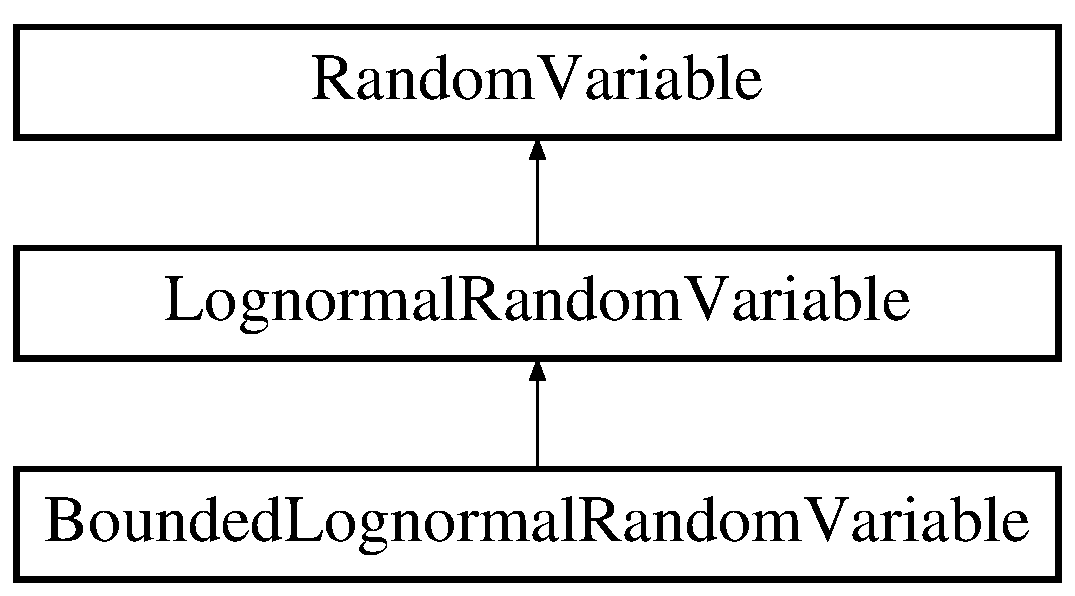
\includegraphics[height=3.000000cm]{classPecos_1_1LognormalRandomVariable}
\end{center}
\end{figure}
\subsection*{Public Member Functions}
\begin{DoxyCompactItemize}
\item 
\hyperlink{classPecos_1_1LognormalRandomVariable_ad3294d11bef887ebfa7ef7afe8079736}{Lognormal\+Random\+Variable} ()\label{classPecos_1_1LognormalRandomVariable_ad3294d11bef887ebfa7ef7afe8079736}

\begin{DoxyCompactList}\small\item\em constructor \end{DoxyCompactList}\item 
\hyperlink{classPecos_1_1LognormalRandomVariable_a1e995a66d32583f8e824b09895694e43}{Lognormal\+Random\+Variable} (Real lambda, Real zeta)\label{classPecos_1_1LognormalRandomVariable_a1e995a66d32583f8e824b09895694e43}

\begin{DoxyCompactList}\small\item\em alternate constructor \end{DoxyCompactList}\item 
\hyperlink{classPecos_1_1LognormalRandomVariable_a207213857452540982f1067d556b58f3}{$\sim$\+Lognormal\+Random\+Variable} ()\label{classPecos_1_1LognormalRandomVariable_a207213857452540982f1067d556b58f3}

\begin{DoxyCompactList}\small\item\em destructor \end{DoxyCompactList}\item 
Real \hyperlink{classPecos_1_1LognormalRandomVariable_addd564e7f4f314e12d38df74d845f0d8}{cdf} (Real x) const \label{classPecos_1_1LognormalRandomVariable_addd564e7f4f314e12d38df74d845f0d8}

\begin{DoxyCompactList}\small\item\em return the cumulative distribution function value of the random variable at x \end{DoxyCompactList}\item 
Real \hyperlink{classPecos_1_1LognormalRandomVariable_a23c3b599e7e4788a9a5e9e93c3dbaf4d}{ccdf} (Real x) const \label{classPecos_1_1LognormalRandomVariable_a23c3b599e7e4788a9a5e9e93c3dbaf4d}

\begin{DoxyCompactList}\small\item\em return the complementary cumulative distribution function value of the random variable at x \end{DoxyCompactList}\item 
Real \hyperlink{classPecos_1_1LognormalRandomVariable_a918a1aac05ca349ea5313eebcba46c3e}{inverse\+\_\+cdf} (Real p\+\_\+cdf) const \label{classPecos_1_1LognormalRandomVariable_a918a1aac05ca349ea5313eebcba46c3e}

\begin{DoxyCompactList}\small\item\em return the x value corresponding to a cumulative probability \end{DoxyCompactList}\item 
Real \hyperlink{classPecos_1_1LognormalRandomVariable_afda003a1f59ff6930902cd5c8601f49b}{inverse\+\_\+ccdf} (Real p\+\_\+ccdf) const \label{classPecos_1_1LognormalRandomVariable_afda003a1f59ff6930902cd5c8601f49b}

\begin{DoxyCompactList}\small\item\em return the x value corresponding to a complementary cumulative probability \end{DoxyCompactList}\item 
Real \hyperlink{classPecos_1_1LognormalRandomVariable_a8ec69265f428e17c1707133cb137a819}{pdf} (Real x) const \label{classPecos_1_1LognormalRandomVariable_a8ec69265f428e17c1707133cb137a819}

\begin{DoxyCompactList}\small\item\em return the value of the random variable\textquotesingle{}s probability density function at x \end{DoxyCompactList}\item 
Real \hyperlink{classPecos_1_1LognormalRandomVariable_aaa7ca3718abc034be7629af5594efca0}{pdf\+\_\+gradient} (Real x) const \label{classPecos_1_1LognormalRandomVariable_aaa7ca3718abc034be7629af5594efca0}

\begin{DoxyCompactList}\small\item\em return the gradient of the random variable\textquotesingle{}s probability density function at x \end{DoxyCompactList}\item 
Real \hyperlink{classPecos_1_1LognormalRandomVariable_a514a0abe97269ac6e003f43683d9137e}{pdf\+\_\+hessian} (Real x) const \label{classPecos_1_1LognormalRandomVariable_a514a0abe97269ac6e003f43683d9137e}

\begin{DoxyCompactList}\small\item\em return the hessian of the random variable\textquotesingle{}s probability density function at x \end{DoxyCompactList}\item 
Real \hyperlink{classPecos_1_1LognormalRandomVariable_a6e2b6b6f13eedb2eb1ef3bc455a06392}{log\+\_\+pdf} (Real x) const \label{classPecos_1_1LognormalRandomVariable_a6e2b6b6f13eedb2eb1ef3bc455a06392}

\begin{DoxyCompactList}\small\item\em return the value of the natural log of the random variable\textquotesingle{}s probability density function at x (useful for calculations of log density in Bayesian methods) \end{DoxyCompactList}\item 
Real \hyperlink{classPecos_1_1LognormalRandomVariable_a5ccc16c04690f0c501f44c1ffae2bbd1}{log\+\_\+pdf\+\_\+gradient} (Real x) const \label{classPecos_1_1LognormalRandomVariable_a5ccc16c04690f0c501f44c1ffae2bbd1}

\begin{DoxyCompactList}\small\item\em return the gradient of the natural log of the random variable\textquotesingle{}s probability density function at x (useful for defining M\+C\+MC proposal distributions in Bayesian methods) \end{DoxyCompactList}\item 
Real \hyperlink{classPecos_1_1LognormalRandomVariable_a7b43f26f0f2bcdfef15d87e1f9399b33}{log\+\_\+pdf\+\_\+hessian} (Real x) const \label{classPecos_1_1LognormalRandomVariable_a7b43f26f0f2bcdfef15d87e1f9399b33}

\begin{DoxyCompactList}\small\item\em return the Hessian of the natural log of the random variable\textquotesingle{}s probability density function at x (useful for defining M\+C\+MC proposal distributions in Bayesian methods) \end{DoxyCompactList}\item 
Real \hyperlink{classPecos_1_1LognormalRandomVariable_aa891dab1ae9a225f493e3a0e5032b778}{parameter} (short dist\+\_\+param) const \label{classPecos_1_1LognormalRandomVariable_aa891dab1ae9a225f493e3a0e5032b778}

\begin{DoxyCompactList}\small\item\em return the value of the named distribution parameter \end{DoxyCompactList}\item 
void \hyperlink{classPecos_1_1LognormalRandomVariable_ae8e123224f588aee676d5d56d5ca900d}{parameter} (short dist\+\_\+param, Real val)\label{classPecos_1_1LognormalRandomVariable_ae8e123224f588aee676d5d56d5ca900d}

\begin{DoxyCompactList}\small\item\em update the value of the named distribution parameter \end{DoxyCompactList}\item 
Real \hyperlink{classPecos_1_1LognormalRandomVariable_a962ffe5a3593be370d5c883365c060f4}{mean} () const \label{classPecos_1_1LognormalRandomVariable_a962ffe5a3593be370d5c883365c060f4}

\begin{DoxyCompactList}\small\item\em return the distribution mean \end{DoxyCompactList}\item 
Real \hyperlink{classPecos_1_1LognormalRandomVariable_ae1fff19ce29a79d657043a598523635d}{median} () const \label{classPecos_1_1LognormalRandomVariable_ae1fff19ce29a79d657043a598523635d}

\begin{DoxyCompactList}\small\item\em return the distribution mode \end{DoxyCompactList}\item 
Real \hyperlink{classPecos_1_1LognormalRandomVariable_a72d3d6926edd929cb3f8e12baa655f70}{mode} () const \label{classPecos_1_1LognormalRandomVariable_a72d3d6926edd929cb3f8e12baa655f70}

\begin{DoxyCompactList}\small\item\em return the distribution mode \end{DoxyCompactList}\item 
Real \hyperlink{classPecos_1_1LognormalRandomVariable_a6a4ed9624d511f8a4e4f509c82cb0706}{standard\+\_\+deviation} () const \label{classPecos_1_1LognormalRandomVariable_a6a4ed9624d511f8a4e4f509c82cb0706}

\begin{DoxyCompactList}\small\item\em return the distribution variance \end{DoxyCompactList}\item 
Real \hyperlink{classPecos_1_1LognormalRandomVariable_a4b8b05b2a9af92dad9cc304c2925a4eb}{variance} () const \label{classPecos_1_1LognormalRandomVariable_a4b8b05b2a9af92dad9cc304c2925a4eb}

\begin{DoxyCompactList}\small\item\em return the distribution variance \end{DoxyCompactList}\item 
Real\+Real\+Pair \hyperlink{classPecos_1_1LognormalRandomVariable_a4bdb95a8fa5fffaa0de5102f56963cf2}{bounds} () const \label{classPecos_1_1LognormalRandomVariable_a4bdb95a8fa5fffaa0de5102f56963cf2}

\begin{DoxyCompactList}\small\item\em return the distribution lower and upper bounds as a pair \end{DoxyCompactList}\item 
Real \hyperlink{classPecos_1_1LognormalRandomVariable_ae1cf1c07047d7ad9dbb899aa01138d54}{coefficient\+\_\+of\+\_\+variation} () const 
\begin{DoxyCompactList}\small\item\em compute the coefficient of variation (used to compute selected correlation warping factors); defined for semi-\/infinite distributions with nonzero mean (lognormal, exponential, gamma, frechet, weibull) \end{DoxyCompactList}\item 
Real \hyperlink{classPecos_1_1LognormalRandomVariable_a9ee48b3ca93459136b2e73f77873c4aa}{correlation\+\_\+warping\+\_\+factor} (const \hyperlink{classPecos_1_1RandomVariable}{Random\+Variable} \&rv, Real corr) const \label{classPecos_1_1LognormalRandomVariable_a9ee48b3ca93459136b2e73f77873c4aa}

\begin{DoxyCompactList}\small\item\em compute the warping factor for correlation between the current variable and the one passed in (used in \hyperlink{classPecos_1_1NatafTransformation}{Nataf\+Transformation}) \end{DoxyCompactList}\item 
Real \hyperlink{classPecos_1_1LognormalRandomVariable_af889af8adfb262c9b74f573b2a9ffc99}{dx\+\_\+ds} (short dist\+\_\+param, short u\+\_\+type, Real x, Real z) const 
\item 
Real \hyperlink{classPecos_1_1LognormalRandomVariable_af6b5fc528523180bed5fc3008dcea205}{dz\+\_\+ds\+\_\+factor} (short u\+\_\+type, Real x, Real z) const 
\item 
void {\bfseries update} (Real lambda, Real zeta)\label{classPecos_1_1LognormalRandomVariable_ac4eb88bb978b104899ccdb80c58aa6c5}

\end{DoxyCompactItemize}
\subsection*{Static Public Member Functions}
\begin{DoxyCompactItemize}
\item 
static Real {\bfseries pdf} (Real x, Real lambda, Real zeta)\label{classPecos_1_1LognormalRandomVariable_a1d84a4e8006cb3c70d737f7738d31824}

\item 
static Real {\bfseries cdf} (Real x, Real lambda, Real zeta)\label{classPecos_1_1LognormalRandomVariable_a31cde087e0c30b3217524c890973eac3}

\item 
static void {\bfseries zeta\+\_\+from\+\_\+error\+\_\+factor} (Real err\+\_\+fact, Real \&zeta)\label{classPecos_1_1LognormalRandomVariable_affca6e2b62db4846f9327a0dac1d7605}

\item 
static void {\bfseries error\+\_\+factor\+\_\+from\+\_\+zeta} (Real zeta, Real \&err\+\_\+fact)\label{classPecos_1_1LognormalRandomVariable_a2b0194f98bf0322210b6743e5376c2f9}

\item 
static void {\bfseries std\+\_\+deviation\+\_\+from\+\_\+error\+\_\+factor} (Real \hyperlink{classPecos_1_1LognormalRandomVariable_a962ffe5a3593be370d5c883365c060f4}{mean}, Real err\+\_\+fact, Real \&std\+\_\+dev)\label{classPecos_1_1LognormalRandomVariable_adf4688894a208bc0bdc2b69fe3da9a4b}

\item 
static void {\bfseries error\+\_\+factor\+\_\+from\+\_\+std\+\_\+deviation} (Real \hyperlink{classPecos_1_1LognormalRandomVariable_a962ffe5a3593be370d5c883365c060f4}{mean}, Real std\+\_\+dev, Real \&err\+\_\+fact)\label{classPecos_1_1LognormalRandomVariable_a69741ef2cd4a868094313bca4a6f11fa}

\item 
static void {\bfseries moments\+\_\+from\+\_\+params} (Real lambda, Real zeta, Real \&\hyperlink{classPecos_1_1LognormalRandomVariable_a962ffe5a3593be370d5c883365c060f4}{mean}, Real \&std\+\_\+dev)\label{classPecos_1_1LognormalRandomVariable_af64ca09c64d690373f0b2dda2dc36326}

\item 
static void {\bfseries zeta\+\_\+sq\+\_\+from\+\_\+moments} (Real \hyperlink{classPecos_1_1LognormalRandomVariable_a962ffe5a3593be370d5c883365c060f4}{mean}, Real std\+\_\+dev, Real \&zeta\+\_\+sq)\label{classPecos_1_1LognormalRandomVariable_a880724c18b1f5c7aa8ad321b219aabb8}

\item 
static void {\bfseries params\+\_\+from\+\_\+moments} (Real \hyperlink{classPecos_1_1LognormalRandomVariable_a962ffe5a3593be370d5c883365c060f4}{mean}, Real std\+\_\+dev, Real \&lambda, Real \&zeta)\label{classPecos_1_1LognormalRandomVariable_a9554a4692a4475ef049f918a1ebcb17f}

\end{DoxyCompactItemize}
\subsection*{Protected Attributes}
\begin{DoxyCompactItemize}
\item 
Real \hyperlink{classPecos_1_1LognormalRandomVariable_a8e90f06d80ffac45a920a673fe62cde2}{ln\+Lambda}\label{classPecos_1_1LognormalRandomVariable_a8e90f06d80ffac45a920a673fe62cde2}

\begin{DoxyCompactList}\small\item\em lambda parameter for lognormal random variable \end{DoxyCompactList}\item 
Real \hyperlink{classPecos_1_1LognormalRandomVariable_ad5359cff7648ac26810956b33568cdf1}{ln\+Zeta}\label{classPecos_1_1LognormalRandomVariable_ad5359cff7648ac26810956b33568cdf1}

\begin{DoxyCompactList}\small\item\em zeta parameter for lognormal random variable \end{DoxyCompactList}\end{DoxyCompactItemize}
\subsection*{Additional Inherited Members}


\subsection{Detailed Description}
Derived random variable class for lognormal random variables. 

Manages lambda and zeta (mean and std deviation of underlying normal distribution). 

\subsection{Member Function Documentation}
\index{Pecos\+::\+Lognormal\+Random\+Variable@{Pecos\+::\+Lognormal\+Random\+Variable}!coefficient\+\_\+of\+\_\+variation@{coefficient\+\_\+of\+\_\+variation}}
\index{coefficient\+\_\+of\+\_\+variation@{coefficient\+\_\+of\+\_\+variation}!Pecos\+::\+Lognormal\+Random\+Variable@{Pecos\+::\+Lognormal\+Random\+Variable}}
\subsubsection[{\texorpdfstring{coefficient\+\_\+of\+\_\+variation() const }{coefficient_of_variation() const }}]{\setlength{\rightskip}{0pt plus 5cm}Real coefficient\+\_\+of\+\_\+variation (
\begin{DoxyParamCaption}
{}
\end{DoxyParamCaption}
) const\hspace{0.3cm}{\ttfamily [inline]}, {\ttfamily [virtual]}}\label{classPecos_1_1LognormalRandomVariable_ae1cf1c07047d7ad9dbb899aa01138d54}


compute the coefficient of variation (used to compute selected correlation warping factors); defined for semi-\/infinite distributions with nonzero mean (lognormal, exponential, gamma, frechet, weibull) 

default is only overridden when more efficient to compute together 

Reimplemented from \hyperlink{classPecos_1_1RandomVariable_ae1cf1c07047d7ad9dbb899aa01138d54}{Random\+Variable}.



References Lognormal\+Random\+Variable\+::correlation\+\_\+warping\+\_\+factor(), and Lognormal\+Random\+Variable\+::ln\+Zeta.



Referenced by Lognormal\+Random\+Variable\+::correlation\+\_\+warping\+\_\+factor().

\index{Pecos\+::\+Lognormal\+Random\+Variable@{Pecos\+::\+Lognormal\+Random\+Variable}!dx\+\_\+ds@{dx\+\_\+ds}}
\index{dx\+\_\+ds@{dx\+\_\+ds}!Pecos\+::\+Lognormal\+Random\+Variable@{Pecos\+::\+Lognormal\+Random\+Variable}}
\subsubsection[{\texorpdfstring{dx\+\_\+ds(short dist\+\_\+param, short u\+\_\+type, Real x, Real z) const }{dx_ds(short dist_param, short u_type, Real x, Real z) const }}]{\setlength{\rightskip}{0pt plus 5cm}Real dx\+\_\+ds (
\begin{DoxyParamCaption}
\item[{short}]{dist\+\_\+param, }
\item[{short}]{u\+\_\+type, }
\item[{Real}]{x, }
\item[{Real}]{z}
\end{DoxyParamCaption}
) const\hspace{0.3cm}{\ttfamily [inline]}, {\ttfamily [virtual]}}\label{classPecos_1_1LognormalRandomVariable_af889af8adfb262c9b74f573b2a9ffc99}
dx/ds is derived by differentiating \hyperlink{classPecos_1_1NatafTransformation_a5feeecf846fc017c5a28eccb4e955dc1}{Nataf\+Transformation\+::trans\+\_\+\+Z\+\_\+to\+\_\+\+X()} with respect to distribution parameter s. dz/ds is zero if uncorrelated, while \hyperlink{classPecos_1_1LognormalRandomVariable_af6b5fc528523180bed5fc3008dcea205}{dz\+\_\+ds\+\_\+factor()} manages contributions in the correlated case. 

Reimplemented from \hyperlink{classPecos_1_1RandomVariable_af889af8adfb262c9b74f573b2a9ffc99}{Random\+Variable}.



References Lognormal\+Random\+Variable\+::dz\+\_\+ds\+\_\+factor(), Lognormal\+Random\+Variable\+::ln\+Lambda, Lognormal\+Random\+Variable\+::ln\+Zeta, and Lognormal\+Random\+Variable\+::mean().



Referenced by Lognormal\+Random\+Variable\+::correlation\+\_\+warping\+\_\+factor().

\index{Pecos\+::\+Lognormal\+Random\+Variable@{Pecos\+::\+Lognormal\+Random\+Variable}!dz\+\_\+ds\+\_\+factor@{dz\+\_\+ds\+\_\+factor}}
\index{dz\+\_\+ds\+\_\+factor@{dz\+\_\+ds\+\_\+factor}!Pecos\+::\+Lognormal\+Random\+Variable@{Pecos\+::\+Lognormal\+Random\+Variable}}
\subsubsection[{\texorpdfstring{dz\+\_\+ds\+\_\+factor(short u\+\_\+type, Real x, Real z) const }{dz_ds_factor(short u_type, Real x, Real z) const }}]{\setlength{\rightskip}{0pt plus 5cm}Real dz\+\_\+ds\+\_\+factor (
\begin{DoxyParamCaption}
\item[{short}]{u\+\_\+type, }
\item[{Real}]{x, }
\item[{Real}]{z}
\end{DoxyParamCaption}
) const\hspace{0.3cm}{\ttfamily [inline]}, {\ttfamily [virtual]}}\label{classPecos_1_1LognormalRandomVariable_af6b5fc528523180bed5fc3008dcea205}
dx/ds is derived by differentiating \hyperlink{classPecos_1_1NatafTransformation_a5feeecf846fc017c5a28eccb4e955dc1}{Nataf\+Transformation\+::trans\+\_\+\+Z\+\_\+to\+\_\+\+X()} with respect to distribution parameter s. For the uncorrelated case, u and z are constants. For the correlated case, u is a constant, but z(s) = L(s) u due to Nataf dependence on s and dz/ds = d\+L/ds u. 

Reimplemented from \hyperlink{classPecos_1_1RandomVariable_af6b5fc528523180bed5fc3008dcea205}{Random\+Variable}.



References Lognormal\+Random\+Variable\+::cdf(), Lognormal\+Random\+Variable\+::ln\+Lambda, Lognormal\+Random\+Variable\+::ln\+Zeta, Lognormal\+Random\+Variable\+::mean(), and Lognormal\+Random\+Variable\+::pdf().



Referenced by Lognormal\+Random\+Variable\+::dx\+\_\+ds().



The documentation for this class was generated from the following file\+:\begin{DoxyCompactItemize}
\item 
Lognormal\+Random\+Variable.\+hpp\end{DoxyCompactItemize}

\section{Loguniform\+Random\+Variable Class Reference}
\label{classPecos_1_1LoguniformRandomVariable}\index{Loguniform\+Random\+Variable@{Loguniform\+Random\+Variable}}


Derived random variable class for loguniform random variables.  


Inheritance diagram for Loguniform\+Random\+Variable\+:\begin{figure}[H]
\begin{center}
\leavevmode
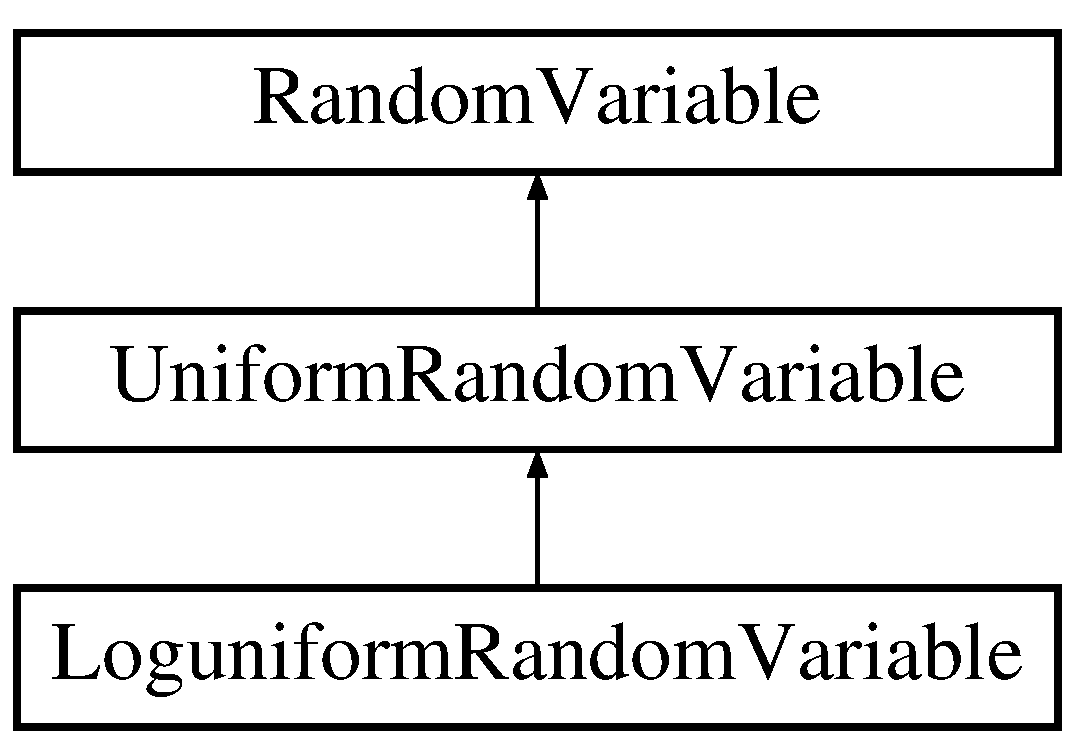
\includegraphics[height=3.000000cm]{classPecos_1_1LoguniformRandomVariable}
\end{center}
\end{figure}
\subsection*{Public Member Functions}
\begin{DoxyCompactItemize}
\item 
\hyperlink{classPecos_1_1LoguniformRandomVariable_a2a04989ce29e747860c267f08dec5b0d}{Loguniform\+Random\+Variable} ()\label{classPecos_1_1LoguniformRandomVariable_a2a04989ce29e747860c267f08dec5b0d}

\begin{DoxyCompactList}\small\item\em default constructor \end{DoxyCompactList}\item 
\hyperlink{classPecos_1_1LoguniformRandomVariable_af2c7e96e0f689a9061ab515206e09cfd}{Loguniform\+Random\+Variable} (Real lwr, Real upr)\label{classPecos_1_1LoguniformRandomVariable_af2c7e96e0f689a9061ab515206e09cfd}

\begin{DoxyCompactList}\small\item\em alternate constructor \end{DoxyCompactList}\item 
\hyperlink{classPecos_1_1LoguniformRandomVariable_a87d670be59e313e45b381b6882e40be9}{$\sim$\+Loguniform\+Random\+Variable} ()\label{classPecos_1_1LoguniformRandomVariable_a87d670be59e313e45b381b6882e40be9}

\begin{DoxyCompactList}\small\item\em destructor \end{DoxyCompactList}\item 
Real \hyperlink{classPecos_1_1LoguniformRandomVariable_addd564e7f4f314e12d38df74d845f0d8}{cdf} (Real x) const \label{classPecos_1_1LoguniformRandomVariable_addd564e7f4f314e12d38df74d845f0d8}

\begin{DoxyCompactList}\small\item\em return the cumulative distribution function value of the random variable at x \end{DoxyCompactList}\item 
Real \hyperlink{classPecos_1_1LoguniformRandomVariable_a23c3b599e7e4788a9a5e9e93c3dbaf4d}{ccdf} (Real x) const \label{classPecos_1_1LoguniformRandomVariable_a23c3b599e7e4788a9a5e9e93c3dbaf4d}

\begin{DoxyCompactList}\small\item\em return the complementary cumulative distribution function value of the random variable at x \end{DoxyCompactList}\item 
Real \hyperlink{classPecos_1_1LoguniformRandomVariable_a918a1aac05ca349ea5313eebcba46c3e}{inverse\+\_\+cdf} (Real p\+\_\+cdf) const \label{classPecos_1_1LoguniformRandomVariable_a918a1aac05ca349ea5313eebcba46c3e}

\begin{DoxyCompactList}\small\item\em return the x value corresponding to a cumulative probability \end{DoxyCompactList}\item 
Real \hyperlink{classPecos_1_1LoguniformRandomVariable_afda003a1f59ff6930902cd5c8601f49b}{inverse\+\_\+ccdf} (Real p\+\_\+ccdf) const \label{classPecos_1_1LoguniformRandomVariable_afda003a1f59ff6930902cd5c8601f49b}

\begin{DoxyCompactList}\small\item\em return the x value corresponding to a complementary cumulative probability \end{DoxyCompactList}\item 
Real \hyperlink{classPecos_1_1LoguniformRandomVariable_a8ec69265f428e17c1707133cb137a819}{pdf} (Real x) const \label{classPecos_1_1LoguniformRandomVariable_a8ec69265f428e17c1707133cb137a819}

\begin{DoxyCompactList}\small\item\em return the value of the random variable\textquotesingle{}s probability density function at x \end{DoxyCompactList}\item 
Real \hyperlink{classPecos_1_1LoguniformRandomVariable_aaa7ca3718abc034be7629af5594efca0}{pdf\+\_\+gradient} (Real x) const \label{classPecos_1_1LoguniformRandomVariable_aaa7ca3718abc034be7629af5594efca0}

\begin{DoxyCompactList}\small\item\em return the gradient of the random variable\textquotesingle{}s probability density function at x \end{DoxyCompactList}\item 
Real \hyperlink{classPecos_1_1LoguniformRandomVariable_a514a0abe97269ac6e003f43683d9137e}{pdf\+\_\+hessian} (Real x) const \label{classPecos_1_1LoguniformRandomVariable_a514a0abe97269ac6e003f43683d9137e}

\begin{DoxyCompactList}\small\item\em return the hessian of the random variable\textquotesingle{}s probability density function at x \end{DoxyCompactList}\item 
Real \hyperlink{classPecos_1_1LoguniformRandomVariable_aa891dab1ae9a225f493e3a0e5032b778}{parameter} (short dist\+\_\+param) const \label{classPecos_1_1LoguniformRandomVariable_aa891dab1ae9a225f493e3a0e5032b778}

\begin{DoxyCompactList}\small\item\em return the value of the named distribution parameter \end{DoxyCompactList}\item 
void \hyperlink{classPecos_1_1LoguniformRandomVariable_ae8e123224f588aee676d5d56d5ca900d}{parameter} (short dist\+\_\+param, Real val)\label{classPecos_1_1LoguniformRandomVariable_ae8e123224f588aee676d5d56d5ca900d}

\begin{DoxyCompactList}\small\item\em update the value of the named distribution parameter \end{DoxyCompactList}\item 
Real \hyperlink{classPecos_1_1LoguniformRandomVariable_a962ffe5a3593be370d5c883365c060f4}{mean} () const \label{classPecos_1_1LoguniformRandomVariable_a962ffe5a3593be370d5c883365c060f4}

\begin{DoxyCompactList}\small\item\em return the distribution mean \end{DoxyCompactList}\item 
Real \hyperlink{classPecos_1_1LoguniformRandomVariable_ae1fff19ce29a79d657043a598523635d}{median} () const \label{classPecos_1_1LoguniformRandomVariable_ae1fff19ce29a79d657043a598523635d}

\begin{DoxyCompactList}\small\item\em return the distribution mode \end{DoxyCompactList}\item 
Real \hyperlink{classPecos_1_1LoguniformRandomVariable_a72d3d6926edd929cb3f8e12baa655f70}{mode} () const \label{classPecos_1_1LoguniformRandomVariable_a72d3d6926edd929cb3f8e12baa655f70}

\begin{DoxyCompactList}\small\item\em return the distribution mode \end{DoxyCompactList}\item 
Real \hyperlink{classPecos_1_1LoguniformRandomVariable_a6a4ed9624d511f8a4e4f509c82cb0706}{standard\+\_\+deviation} () const \label{classPecos_1_1LoguniformRandomVariable_a6a4ed9624d511f8a4e4f509c82cb0706}

\begin{DoxyCompactList}\small\item\em return the distribution variance \end{DoxyCompactList}\item 
Real \hyperlink{classPecos_1_1LoguniformRandomVariable_a4b8b05b2a9af92dad9cc304c2925a4eb}{variance} () const \label{classPecos_1_1LoguniformRandomVariable_a4b8b05b2a9af92dad9cc304c2925a4eb}

\begin{DoxyCompactList}\small\item\em return the distribution variance \end{DoxyCompactList}\item 
Real \hyperlink{classPecos_1_1LoguniformRandomVariable_af889af8adfb262c9b74f573b2a9ffc99}{dx\+\_\+ds} (short dist\+\_\+param, short u\+\_\+type, Real x, Real z) const 
\item 
Real \hyperlink{classPecos_1_1LoguniformRandomVariable_af6b5fc528523180bed5fc3008dcea205}{dz\+\_\+ds\+\_\+factor} (short u\+\_\+type, Real x, Real z) const 
\end{DoxyCompactItemize}
\subsection*{Static Public Member Functions}
\begin{DoxyCompactItemize}
\item 
static Real {\bfseries pdf} (Real x, Real lwr, Real upr)\label{classPecos_1_1LoguniformRandomVariable_a041c03ed04c71a52e2e966f6456f60ac}

\item 
static Real {\bfseries cdf} (Real x, Real lwr, Real upr)\label{classPecos_1_1LoguniformRandomVariable_aede5e67889821db4de4440970772d0a0}

\item 
static void {\bfseries moments\+\_\+from\+\_\+params} (Real lwr, Real upr, Real \&\hyperlink{classPecos_1_1LoguniformRandomVariable_a962ffe5a3593be370d5c883365c060f4}{mean}, Real \&std\+\_\+dev)\label{classPecos_1_1LoguniformRandomVariable_aa2fe5db8e1960533b3d1389dcfdd39a8}

\end{DoxyCompactItemize}
\subsection*{Additional Inherited Members}


\subsection{Detailed Description}
Derived random variable class for loguniform random variables. 

Manages lower and upper bounds. See S\+A\+N\+D98-\/0210 L\+HS manual, pp. 43-\/44. 

\subsection{Member Function Documentation}
\index{Pecos\+::\+Loguniform\+Random\+Variable@{Pecos\+::\+Loguniform\+Random\+Variable}!dx\+\_\+ds@{dx\+\_\+ds}}
\index{dx\+\_\+ds@{dx\+\_\+ds}!Pecos\+::\+Loguniform\+Random\+Variable@{Pecos\+::\+Loguniform\+Random\+Variable}}
\subsubsection[{\texorpdfstring{dx\+\_\+ds(short dist\+\_\+param, short u\+\_\+type, Real x, Real z) const }{dx_ds(short dist_param, short u_type, Real x, Real z) const }}]{\setlength{\rightskip}{0pt plus 5cm}Real dx\+\_\+ds (
\begin{DoxyParamCaption}
\item[{short}]{dist\+\_\+param, }
\item[{short}]{u\+\_\+type, }
\item[{Real}]{x, }
\item[{Real}]{z}
\end{DoxyParamCaption}
) const\hspace{0.3cm}{\ttfamily [inline]}, {\ttfamily [virtual]}}\label{classPecos_1_1LoguniformRandomVariable_af889af8adfb262c9b74f573b2a9ffc99}
dx/ds is derived by differentiating \hyperlink{classPecos_1_1NatafTransformation_a5feeecf846fc017c5a28eccb4e955dc1}{Nataf\+Transformation\+::trans\+\_\+\+Z\+\_\+to\+\_\+\+X()} with respect to distribution parameter s. dz/ds is zero if uncorrelated, while \hyperlink{classPecos_1_1LoguniformRandomVariable_af6b5fc528523180bed5fc3008dcea205}{dz\+\_\+ds\+\_\+factor()} manages contributions in the correlated case. 

Reimplemented from \hyperlink{classPecos_1_1RandomVariable_af889af8adfb262c9b74f573b2a9ffc99}{Random\+Variable}.



References Loguniform\+Random\+Variable\+::dz\+\_\+ds\+\_\+factor(), Uniform\+Random\+Variable\+::lower\+Bnd, Normal\+Random\+Variable\+::std\+\_\+cdf(), and Uniform\+Random\+Variable\+::upper\+Bnd.



Referenced by Loguniform\+Random\+Variable\+::variance().

\index{Pecos\+::\+Loguniform\+Random\+Variable@{Pecos\+::\+Loguniform\+Random\+Variable}!dz\+\_\+ds\+\_\+factor@{dz\+\_\+ds\+\_\+factor}}
\index{dz\+\_\+ds\+\_\+factor@{dz\+\_\+ds\+\_\+factor}!Pecos\+::\+Loguniform\+Random\+Variable@{Pecos\+::\+Loguniform\+Random\+Variable}}
\subsubsection[{\texorpdfstring{dz\+\_\+ds\+\_\+factor(short u\+\_\+type, Real x, Real z) const }{dz_ds_factor(short u_type, Real x, Real z) const }}]{\setlength{\rightskip}{0pt plus 5cm}Real dz\+\_\+ds\+\_\+factor (
\begin{DoxyParamCaption}
\item[{short}]{u\+\_\+type, }
\item[{Real}]{x, }
\item[{Real}]{z}
\end{DoxyParamCaption}
) const\hspace{0.3cm}{\ttfamily [inline]}, {\ttfamily [virtual]}}\label{classPecos_1_1LoguniformRandomVariable_af6b5fc528523180bed5fc3008dcea205}
dx/ds is derived by differentiating \hyperlink{classPecos_1_1NatafTransformation_a5feeecf846fc017c5a28eccb4e955dc1}{Nataf\+Transformation\+::trans\+\_\+\+Z\+\_\+to\+\_\+\+X()} with respect to distribution parameter s. For the uncorrelated case, u and z are constants. For the correlated case, u is a constant, but z(s) = L(s) u due to Nataf dependence on s and dz/ds = d\+L/ds u. 

Reimplemented from \hyperlink{classPecos_1_1RandomVariable_af6b5fc528523180bed5fc3008dcea205}{Random\+Variable}.



References Loguniform\+Random\+Variable\+::cdf(), Uniform\+Random\+Variable\+::lower\+Bnd, Loguniform\+Random\+Variable\+::mean(), Loguniform\+Random\+Variable\+::pdf(), Pecos\+::range(), Normal\+Random\+Variable\+::std\+\_\+pdf(), and Uniform\+Random\+Variable\+::upper\+Bnd.



Referenced by Loguniform\+Random\+Variable\+::dx\+\_\+ds().



The documentation for this class was generated from the following file\+:\begin{DoxyCompactItemize}
\item 
Loguniform\+Random\+Variable.\+hpp\end{DoxyCompactItemize}

\section{Meixner\+Orthog\+Polynomial Class Reference}
\label{classPecos_1_1MeixnerOrthogPolynomial}\index{Meixner\+Orthog\+Polynomial@{Meixner\+Orthog\+Polynomial}}


Derived orthogonal polynomial class for Meixner polynomials.  


Inheritance diagram for Meixner\+Orthog\+Polynomial\+:\begin{figure}[H]
\begin{center}
\leavevmode
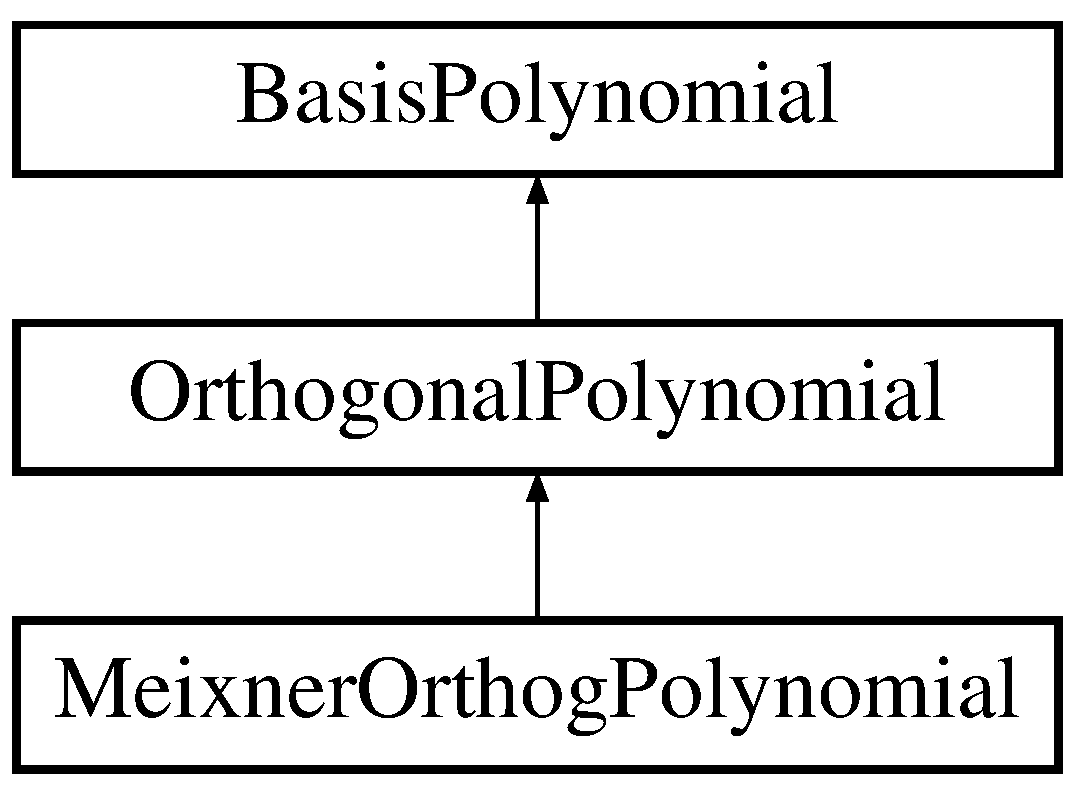
\includegraphics[height=3.000000cm]{classPecos_1_1MeixnerOrthogPolynomial}
\end{center}
\end{figure}
\subsection*{Public Member Functions}
\begin{DoxyCompactItemize}
\item 
\hyperlink{classPecos_1_1MeixnerOrthogPolynomial_a625f09ddd19a12e148fbee78be7bc642}{Meixner\+Orthog\+Polynomial} ()\label{classPecos_1_1MeixnerOrthogPolynomial_a625f09ddd19a12e148fbee78be7bc642}

\begin{DoxyCompactList}\small\item\em default constructor \end{DoxyCompactList}\item 
\hyperlink{classPecos_1_1MeixnerOrthogPolynomial_ae93759041d0eda3b1a696969097ab2b8}{$\sim$\+Meixner\+Orthog\+Polynomial} ()\label{classPecos_1_1MeixnerOrthogPolynomial_ae93759041d0eda3b1a696969097ab2b8}

\begin{DoxyCompactList}\small\item\em destructor \end{DoxyCompactList}\end{DoxyCompactItemize}
\subsection*{Protected Member Functions}
\begin{DoxyCompactItemize}
\item 
Real \hyperlink{classPecos_1_1MeixnerOrthogPolynomial_a8792a858ac05a2158880e876f9da2019}{type1\+\_\+value} (Real x, unsigned short order)
\begin{DoxyCompactList}\small\item\em retrieve the value of the n\+\_\+th type 1 polynomial for a given parameter x using traditional characteristic polynomial formulation \end{DoxyCompactList}\item 
Real \hyperlink{classPecos_1_1MeixnerOrthogPolynomial_a997bdeddf670667c476513fcacc779ca}{alpha\+\_\+polynomial} () const \label{classPecos_1_1MeixnerOrthogPolynomial_a997bdeddf670667c476513fcacc779ca}

\begin{DoxyCompactList}\small\item\em return alpha\+Poly \end{DoxyCompactList}\item 
Real \hyperlink{classPecos_1_1MeixnerOrthogPolynomial_a22bfc4209dec76716ef51648e945469a}{beta\+\_\+polynomial} () const \label{classPecos_1_1MeixnerOrthogPolynomial_a22bfc4209dec76716ef51648e945469a}

\begin{DoxyCompactList}\small\item\em return beta\+Poly \end{DoxyCompactList}\item 
void \hyperlink{classPecos_1_1MeixnerOrthogPolynomial_aeeb4ce11a8d413209be1ec08eced8728}{alpha\+\_\+stat} (Real alpha)\label{classPecos_1_1MeixnerOrthogPolynomial_aeeb4ce11a8d413209be1ec08eced8728}

\begin{DoxyCompactList}\small\item\em set alpha\+Stat (probability per trial) \end{DoxyCompactList}\item 
void \hyperlink{classPecos_1_1MeixnerOrthogPolynomial_a7f9584e538ee1574bd4d8d1afb622ed6}{beta\+\_\+stat} (Real beta)\label{classPecos_1_1MeixnerOrthogPolynomial_a7f9584e538ee1574bd4d8d1afb622ed6}

\begin{DoxyCompactList}\small\item\em set beta\+Stat (num trials) \end{DoxyCompactList}\end{DoxyCompactItemize}
\subsection*{Private Attributes}
\begin{DoxyCompactItemize}
\item 
Real \hyperlink{classPecos_1_1MeixnerOrthogPolynomial_a11666846719189915a02ac6f1f96e393}{alpha\+Poly}\label{classPecos_1_1MeixnerOrthogPolynomial_a11666846719189915a02ac6f1f96e393}

\begin{DoxyCompactList}\small\item\em the probability of a \char`\"{}success\char`\"{} for each experiment \end{DoxyCompactList}\item 
Real \hyperlink{classPecos_1_1MeixnerOrthogPolynomial_a96c0b0201ca445f95be14ec035b595cb}{beta\+Poly}\label{classPecos_1_1MeixnerOrthogPolynomial_a96c0b0201ca445f95be14ec035b595cb}

\begin{DoxyCompactList}\small\item\em the number of failures allowed \end{DoxyCompactList}\end{DoxyCompactItemize}
\subsection*{Additional Inherited Members}


\subsection{Detailed Description}
Derived orthogonal polynomial class for Meixner polynomials. 

The \hyperlink{classPecos_1_1MeixnerOrthogPolynomial}{Meixner\+Orthog\+Polynomial} class evaluates a univariate Meixner polynomial M$^\wedge$(c,Beta)\+\_\+n of a particular order. These polynomials are orthogonal with respect to the weight function

(k+r-\/1 choose k)$\ast$p$^\wedge$k$\ast$(1-\/p)$^\wedge$n, where p is the the probability of success of a trial, n is the number of total successes and k is the trial number. The geometric distribution (n==1) is a special case of the negative binomial distribution. This corresponds to the negative binomial probability mass function. See appendix in Xiu \& Karniadakis, Siam J. Sci. Comp., v24, n2, pp. 619-\/644, 2002 for more details. 

\subsection{Member Function Documentation}
\index{Pecos\+::\+Meixner\+Orthog\+Polynomial@{Pecos\+::\+Meixner\+Orthog\+Polynomial}!type1\+\_\+value@{type1\+\_\+value}}
\index{type1\+\_\+value@{type1\+\_\+value}!Pecos\+::\+Meixner\+Orthog\+Polynomial@{Pecos\+::\+Meixner\+Orthog\+Polynomial}}
\subsubsection[{\texorpdfstring{type1\+\_\+value(\+Real x, unsigned short order)}{type1_value(Real x, unsigned short order)}}]{\setlength{\rightskip}{0pt plus 5cm}Real type1\+\_\+value (
\begin{DoxyParamCaption}
\item[{Real}]{x, }
\item[{unsigned short}]{n}
\end{DoxyParamCaption}
)\hspace{0.3cm}{\ttfamily [protected]}, {\ttfamily [virtual]}}\label{classPecos_1_1MeixnerOrthogPolynomial_a8792a858ac05a2158880e876f9da2019}


retrieve the value of the n\+\_\+th type 1 polynomial for a given parameter x using traditional characteristic polynomial formulation 

For orthogonal polynomials, n specifies the order of the polynomial, whereas for interpolation polynomials, it identifies the interpolant for the n-\/th point. 

Reimplemented from \hyperlink{classPecos_1_1BasisPolynomial_a1fab871e99cec3a1933a2b1e9ed8a625}{Basis\+Polynomial}.



References Meixner\+Orthog\+Polynomial\+::alpha\+Poly, and Meixner\+Orthog\+Polynomial\+::beta\+Poly.



The documentation for this class was generated from the following files\+:\begin{DoxyCompactItemize}
\item 
Meixner\+Orthog\+Polynomial.\+hpp\item 
Meixner\+Orthog\+Polynomial.\+cpp\end{DoxyCompactItemize}

\section{Nataf\+Transformation Class Reference}
\label{classPecos_1_1NatafTransformation}\index{Nataf\+Transformation@{Nataf\+Transformation}}


Class for Nataf nonlinear distribution transformation.  


Inheritance diagram for Nataf\+Transformation\+:\begin{figure}[H]
\begin{center}
\leavevmode
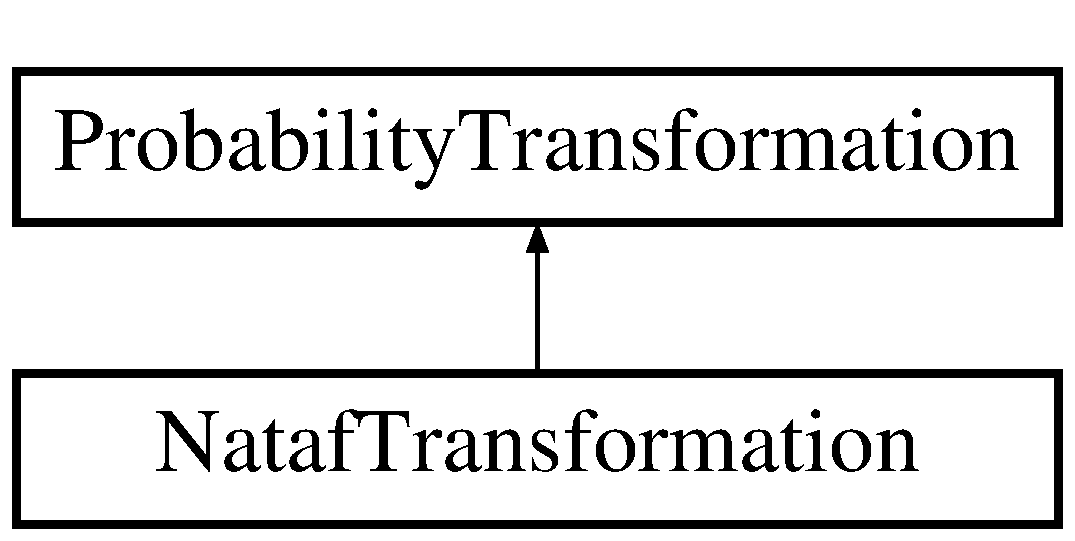
\includegraphics[height=2.000000cm]{classPecos_1_1NatafTransformation}
\end{center}
\end{figure}
\subsection*{Public Member Functions}
\begin{DoxyCompactItemize}
\item 
\hyperlink{classPecos_1_1NatafTransformation_ad619eb82703cf3598c33964ce4f179d1}{Nataf\+Transformation} ()\label{classPecos_1_1NatafTransformation_ad619eb82703cf3598c33964ce4f179d1}

\begin{DoxyCompactList}\small\item\em constructor \end{DoxyCompactList}\item 
\hyperlink{classPecos_1_1NatafTransformation_af6d53b385a804858e3e0d9b4e419f5ef}{$\sim$\+Nataf\+Transformation} ()\label{classPecos_1_1NatafTransformation_af6d53b385a804858e3e0d9b4e419f5ef}

\begin{DoxyCompactList}\small\item\em destructor \end{DoxyCompactList}\end{DoxyCompactItemize}
\subsection*{Protected Member Functions}
\begin{DoxyCompactItemize}
\item 
void \hyperlink{classPecos_1_1NatafTransformation_a0a84860a9ed0cec52ed100edb49f209c}{trans\+\_\+\+U\+\_\+to\+\_\+X} (const Real\+Vector \&u\+\_\+vars, Real\+Vector \&x\+\_\+vars)
\begin{DoxyCompactList}\small\item\em Transformation routine from u-\/space of uncorrelated standard normal variables to x-\/space of correlated random variables. \end{DoxyCompactList}\item 
void \hyperlink{classPecos_1_1NatafTransformation_a22c3e4ffde57732ffe3cbb7ab5fce86b}{trans\+\_\+\+X\+\_\+to\+\_\+U} (const Real\+Vector \&x\+\_\+vars, Real\+Vector \&u\+\_\+vars)
\begin{DoxyCompactList}\small\item\em Transformation routine from x-\/space of correlated random variables to u-\/space of uncorrelated standard normal variables. \end{DoxyCompactList}\item 
void \hyperlink{classPecos_1_1NatafTransformation_a1be77b7133acb8e63d2c6957b9eb6265}{transform\+\_\+correlations} ()
\begin{DoxyCompactList}\small\item\em As part of the Nataf distribution model (Der Kiureghian \& Liu, 1986), this procedure modifies the user-\/specified correlation matrix (corr\+MatrixX) to account for correlation warping from the nonlinear X-\/$>$Z transformation and performs a Cholesky factorization to create corr\+Cholesky\+FactorZ. \end{DoxyCompactList}\item 
void \hyperlink{classPecos_1_1NatafTransformation_ae96fa589437ca113086aa590ac2e0901}{trans\+\_\+grad\+\_\+\+X\+\_\+to\+\_\+U} (const Real\+Vector \&fn\+\_\+grad\+\_\+x, Real\+Vector \&fn\+\_\+grad\+\_\+u, const Real\+Vector \&x\+\_\+vars, const Sizet\+Array \&x\+\_\+dvv, Sizet\+Multi\+Array\+Const\+View cv\+\_\+ids)
\begin{DoxyCompactList}\small\item\em Transformation routine for gradient vector from x-\/space to u-\/space. \end{DoxyCompactList}\item 
void \hyperlink{classPecos_1_1NatafTransformation_af54120bc359031c6fb812013af1488e1}{trans\+\_\+grad\+\_\+\+X\+\_\+to\+\_\+U} (const Real\+Vector \&fn\+\_\+grad\+\_\+x, Real\+Vector \&fn\+\_\+grad\+\_\+u, const Real\+Matrix \&jacobian\+\_\+xu, const Sizet\+Array \&x\+\_\+dvv, Sizet\+Multi\+Array\+Const\+View cv\+\_\+ids)
\begin{DoxyCompactList}\small\item\em Transformation routine for gradient vector from x-\/space to u-\/space. \end{DoxyCompactList}\item 
void \hyperlink{classPecos_1_1NatafTransformation_ade156a969120a98a9a7c7cab9a96b95a}{trans\+\_\+grad\+\_\+\+X\+\_\+to\+\_\+S} (const Real\+Vector \&fn\+\_\+grad\+\_\+x, Real\+Vector \&fn\+\_\+grad\+\_\+s, const Real\+Vector \&x\+\_\+vars, const Sizet\+Array \&x\+\_\+dvv, Sizet\+Multi\+Array\+Const\+View cv\+\_\+ids, Sizet\+Multi\+Array\+Const\+View acv\+\_\+ids, const Sizet\+Array \&acv\+\_\+map1\+\_\+indices, const Short\+Array \&acv\+\_\+map2\+\_\+targets)
\begin{DoxyCompactList}\small\item\em Transformation routine from x-\/space gradient vector to design space. \end{DoxyCompactList}\item 
void \hyperlink{classPecos_1_1NatafTransformation_a3c3f2d04567b733c649d76da95053349}{trans\+\_\+grad\+\_\+\+X\+\_\+to\+\_\+S} (const Real\+Vector \&fn\+\_\+grad\+\_\+x, Real\+Vector \&fn\+\_\+grad\+\_\+s, const Real\+Matrix \&jacobian\+\_\+xs, const Sizet\+Array \&x\+\_\+dvv, Sizet\+Multi\+Array\+Const\+View cv\+\_\+ids, Sizet\+Multi\+Array\+Const\+View acv\+\_\+ids, const Sizet\+Array \&acv\+\_\+map1\+\_\+indices, const Short\+Array \&acv\+\_\+map2\+\_\+targets)
\begin{DoxyCompactList}\small\item\em Transformation routine from x-\/space gradient vector to design space. \end{DoxyCompactList}\item 
void \hyperlink{classPecos_1_1NatafTransformation_a1c9148d72997a3013aebbb513a998a96}{trans\+\_\+grad\+\_\+\+U\+\_\+to\+\_\+X} (const Real\+Vector \&fn\+\_\+grad\+\_\+u, Real\+Vector \&fn\+\_\+grad\+\_\+x, const Real\+Vector \&x\+\_\+vars, const Sizet\+Array \&x\+\_\+dvv, Sizet\+Multi\+Array\+Const\+View cv\+\_\+ids)
\begin{DoxyCompactList}\small\item\em Transformation routine for gradient vector from u-\/space to x-\/space. \end{DoxyCompactList}\item 
void \hyperlink{classPecos_1_1NatafTransformation_aab090e0e7dac78688cfbde1fe2c80ca1}{trans\+\_\+grad\+\_\+\+U\+\_\+to\+\_\+X} (const Real\+Vector \&fn\+\_\+grad\+\_\+u, Real\+Vector \&fn\+\_\+grad\+\_\+x, const Real\+Matrix \&jacobian\+\_\+ux, const Sizet\+Array \&x\+\_\+dvv, Sizet\+Multi\+Array\+Const\+View cv\+\_\+ids)
\begin{DoxyCompactList}\small\item\em Transformation routine for gradient vector from u-\/space to x-\/space. \end{DoxyCompactList}\item 
void \hyperlink{classPecos_1_1NatafTransformation_a834e672f9ac2f1c28b8f6d2f89d7ac85}{trans\+\_\+hess\+\_\+\+X\+\_\+to\+\_\+U} (const Real\+Sym\+Matrix \&fn\+\_\+hess\+\_\+x, Real\+Sym\+Matrix \&fn\+\_\+hess\+\_\+u, const Real\+Vector \&x\+\_\+vars, const Real\+Vector \&fn\+\_\+grad\+\_\+x, const Sizet\+Array \&x\+\_\+dvv, Sizet\+Multi\+Array\+Const\+View cv\+\_\+ids)
\begin{DoxyCompactList}\small\item\em Transformation routine for Hessian matrix from x-\/space to u-\/space. \end{DoxyCompactList}\item 
void \hyperlink{classPecos_1_1NatafTransformation_ad054ed1ba6cb80d20cad29f0efe7da5a}{trans\+\_\+hess\+\_\+\+X\+\_\+to\+\_\+U} (const Real\+Sym\+Matrix \&fn\+\_\+hess\+\_\+x, Real\+Sym\+Matrix \&fn\+\_\+hess\+\_\+u, const Real\+Matrix \&jacobian\+\_\+xu, const Real\+Sym\+Matrix\+Array \&hessian\+\_\+xu, const Real\+Vector \&fn\+\_\+grad\+\_\+x, const Sizet\+Array \&x\+\_\+dvv, Sizet\+Multi\+Array\+Const\+View cv\+\_\+ids)
\begin{DoxyCompactList}\small\item\em Transformation routine for Hessian matrix from x-\/space to u-\/space. \end{DoxyCompactList}\item 
void \hyperlink{classPecos_1_1NatafTransformation_a8e619029699319ac96359e41a74e8744}{jacobian\+\_\+d\+X\+\_\+dU} (const Real\+Vector \&x\+\_\+vars, Real\+Matrix \&jacobian\+\_\+xu)
\begin{DoxyCompactList}\small\item\em Jacobian of x(u) mapping obtained from d\+X/dZ d\+Z/dU. \end{DoxyCompactList}\item 
void \hyperlink{classPecos_1_1NatafTransformation_aa180d3b929eb6f019015fbbff559c0d9}{jacobian\+\_\+d\+U\+\_\+dX} (const Real\+Vector \&x\+\_\+vars, Real\+Matrix \&jacobian\+\_\+ux)
\begin{DoxyCompactList}\small\item\em Jacobian of u(x) mapping obtained from d\+U/dZ d\+Z/dX. \end{DoxyCompactList}\item 
void \hyperlink{classPecos_1_1NatafTransformation_ae634a57bc8deb15bb17a9699b5035669}{jacobian\+\_\+d\+X\+\_\+dS} (const Real\+Vector \&x\+\_\+vars, Real\+Matrix \&jacobian\+\_\+xs, Sizet\+Multi\+Array\+Const\+View cv\+\_\+ids, Sizet\+Multi\+Array\+Const\+View acv\+\_\+ids, const Sizet\+Array \&acv\+\_\+map1\+\_\+indices, const Short\+Array \&acv\+\_\+map2\+\_\+targets)
\begin{DoxyCompactList}\small\item\em Design Jacobian of x(u,s) mapping obtained from differentiation of \hyperlink{classPecos_1_1NatafTransformation_a0a84860a9ed0cec52ed100edb49f209c}{trans\+\_\+\+U\+\_\+to\+\_\+\+X()} with respect to distribution parameters S. \end{DoxyCompactList}\item 
void \hyperlink{classPecos_1_1NatafTransformation_a6b88718fb820430ebbd87749b27b402a}{hessian\+\_\+d2\+X\+\_\+d\+U2} (const Real\+Vector \&x\+\_\+vars, Real\+Sym\+Matrix\+Array \&hessian\+\_\+xu)
\begin{DoxyCompactList}\small\item\em Hessian of x(u) mapping obtained from d\+Z/d\+U$^\wedge$T d$^\wedge$2\+X/d\+Z$^\wedge$2 d\+Z/dU. \end{DoxyCompactList}\end{DoxyCompactItemize}
\subsection*{Private Member Functions}
\begin{DoxyCompactItemize}
\item 
void \hyperlink{classPecos_1_1NatafTransformation_add8c6a190d982a11a89c893090f7addc}{trans\+\_\+\+U\+\_\+to\+\_\+Z} (const Real\+Vector \&u\+\_\+vars, Real\+Vector \&z\+\_\+vars)
\begin{DoxyCompactList}\small\item\em Transformation routine from u-\/space of uncorrelated standard normal variables to z-\/space of correlated standard normal variables. \end{DoxyCompactList}\item 
void \hyperlink{classPecos_1_1NatafTransformation_a5feeecf846fc017c5a28eccb4e955dc1}{trans\+\_\+\+Z\+\_\+to\+\_\+X} (const Real\+Vector \&z\+\_\+vars, Real\+Vector \&x\+\_\+vars)
\begin{DoxyCompactList}\small\item\em Transformation routine from z-\/space of correlated standard normal variables to x-\/space of correlated random variables. \end{DoxyCompactList}\item 
void \hyperlink{classPecos_1_1NatafTransformation_a4abf7f380d1a3f3b4a42c982286f745f}{trans\+\_\+\+Z\+\_\+to\+\_\+X} (Real z, Real \&x, size\+\_\+t i)
\begin{DoxyCompactList}\small\item\em Transformation routine from a single z-\/space variable to a corresponding x-\/space variable. \end{DoxyCompactList}\item 
void \hyperlink{classPecos_1_1NatafTransformation_a08fa15c70e2b4933fe20a1956df8be45}{trans\+\_\+\+X\+\_\+to\+\_\+Z} (const Real\+Vector \&x\+\_\+vars, Real\+Vector \&z\+\_\+vars)
\begin{DoxyCompactList}\small\item\em Transformation routine from x-\/space of correlated random variables to z-\/space of correlated standard normal variables. \end{DoxyCompactList}\item 
void \hyperlink{classPecos_1_1NatafTransformation_a44ef66f532bfdff2676d6cc5eb57b668}{trans\+\_\+\+X\+\_\+to\+\_\+Z} (Real x, Real \&z, size\+\_\+t i)
\begin{DoxyCompactList}\small\item\em Transformation routine from a single x-\/space random variable to a corresponding z-\/space variable. \end{DoxyCompactList}\item 
void \hyperlink{classPecos_1_1NatafTransformation_a228064f2ee23ccf3fae3c9ead6b173a5}{trans\+\_\+\+Z\+\_\+to\+\_\+U} (Real\+Vector \&z\+\_\+vars, Real\+Vector \&u\+\_\+vars)
\begin{DoxyCompactList}\small\item\em Transformation routine from z-\/space of correlated standard normal variables to u-\/space of uncorrelated standard normal variables. \end{DoxyCompactList}\item 
void \hyperlink{classPecos_1_1NatafTransformation_aea9f6918e7726d5ea6d1484d5eefc4f0}{jacobian\+\_\+d\+X\+\_\+dZ} (const Real\+Vector \&x\+\_\+vars, Real\+Matrix \&jacobian\+\_\+xz)
\begin{DoxyCompactList}\small\item\em Jacobian of x(z) mapping obtained from differentiation of \hyperlink{classPecos_1_1NatafTransformation_a5feeecf846fc017c5a28eccb4e955dc1}{trans\+\_\+\+Z\+\_\+to\+\_\+\+X()} \end{DoxyCompactList}\item 
void \hyperlink{classPecos_1_1NatafTransformation_afe2c6f555bc8e5134f610e503aed26dd}{jacobian\+\_\+d\+Z\+\_\+dX} (const Real\+Vector \&x\+\_\+vars, Real\+Matrix \&jacobian\+\_\+zx)
\begin{DoxyCompactList}\small\item\em Jacobian of z(x) mapping obtained from differentiation of \hyperlink{classPecos_1_1NatafTransformation_a08fa15c70e2b4933fe20a1956df8be45}{trans\+\_\+\+X\+\_\+to\+\_\+\+Z()} \end{DoxyCompactList}\item 
void \hyperlink{classPecos_1_1NatafTransformation_a18dce9172d436bd04d8e32229dbe8c5b}{hessian\+\_\+d2\+X\+\_\+d\+Z2} (const Real\+Vector \&x\+\_\+vars, Real\+Sym\+Matrix\+Array \&hessian\+\_\+xz)
\begin{DoxyCompactList}\small\item\em Hessian of x(z) mapping obtained from differentiation of \hyperlink{classPecos_1_1NatafTransformation_aea9f6918e7726d5ea6d1484d5eefc4f0}{jacobian\+\_\+d\+X\+\_\+d\+Z()} \end{DoxyCompactList}\end{DoxyCompactItemize}
\subsection*{Additional Inherited Members}


\subsection{Detailed Description}
Class for Nataf nonlinear distribution transformation. 

The Nataf transformation occurs in two steps\+: (1) transformation from the original correlated distributions (x-\/space) to correlated standard normals (z-\/space) using C\+DF matching and from correlated standard normals to uncorrelated standard normals (u-\/space) using the inverse Cholesky factor of a modified correlation matrix. 

\subsection{Member Function Documentation}
\index{Pecos\+::\+Nataf\+Transformation@{Pecos\+::\+Nataf\+Transformation}!trans\+\_\+\+U\+\_\+to\+\_\+X@{trans\+\_\+\+U\+\_\+to\+\_\+X}}
\index{trans\+\_\+\+U\+\_\+to\+\_\+X@{trans\+\_\+\+U\+\_\+to\+\_\+X}!Pecos\+::\+Nataf\+Transformation@{Pecos\+::\+Nataf\+Transformation}}
\subsubsection[{\texorpdfstring{trans\+\_\+\+U\+\_\+to\+\_\+\+X(const Real\+Vector \&u\+\_\+vars, Real\+Vector \&x\+\_\+vars)}{trans_U_to_X(const RealVector &u_vars, RealVector &x_vars)}}]{\setlength{\rightskip}{0pt plus 5cm}void trans\+\_\+\+U\+\_\+to\+\_\+X (
\begin{DoxyParamCaption}
\item[{const Real\+Vector \&}]{u\+\_\+vars, }
\item[{Real\+Vector \&}]{x\+\_\+vars}
\end{DoxyParamCaption}
)\hspace{0.3cm}{\ttfamily [protected]}, {\ttfamily [virtual]}}\label{classPecos_1_1NatafTransformation_a0a84860a9ed0cec52ed100edb49f209c}


Transformation routine from u-\/space of uncorrelated standard normal variables to x-\/space of correlated random variables. 

This procedure performs the transformation from u to x space. u\+\_\+vars is the vector of random variables in uncorrelated standard normal space (u-\/space). x\+\_\+vars is the vector of random variables in the original user-\/defined x-\/space. 

Reimplemented from \hyperlink{classPecos_1_1ProbabilityTransformation_a0a84860a9ed0cec52ed100edb49f209c}{Probability\+Transformation}.



References Probability\+Transformation\+::correlation\+FlagX, Nataf\+Transformation\+::trans\+\_\+\+U\+\_\+to\+\_\+\+Z(), and Nataf\+Transformation\+::trans\+\_\+\+Z\+\_\+to\+\_\+\+X().

\index{Pecos\+::\+Nataf\+Transformation@{Pecos\+::\+Nataf\+Transformation}!trans\+\_\+\+X\+\_\+to\+\_\+U@{trans\+\_\+\+X\+\_\+to\+\_\+U}}
\index{trans\+\_\+\+X\+\_\+to\+\_\+U@{trans\+\_\+\+X\+\_\+to\+\_\+U}!Pecos\+::\+Nataf\+Transformation@{Pecos\+::\+Nataf\+Transformation}}
\subsubsection[{\texorpdfstring{trans\+\_\+\+X\+\_\+to\+\_\+\+U(const Real\+Vector \&x\+\_\+vars, Real\+Vector \&u\+\_\+vars)}{trans_X_to_U(const RealVector &x_vars, RealVector &u_vars)}}]{\setlength{\rightskip}{0pt plus 5cm}void trans\+\_\+\+X\+\_\+to\+\_\+U (
\begin{DoxyParamCaption}
\item[{const Real\+Vector \&}]{x\+\_\+vars, }
\item[{Real\+Vector \&}]{u\+\_\+vars}
\end{DoxyParamCaption}
)\hspace{0.3cm}{\ttfamily [protected]}, {\ttfamily [virtual]}}\label{classPecos_1_1NatafTransformation_a22c3e4ffde57732ffe3cbb7ab5fce86b}


Transformation routine from x-\/space of correlated random variables to u-\/space of uncorrelated standard normal variables. 

This procedure performs the transformation from x to u space u\+\_\+vars is the vector of random variables in uncorrelated standard normal space (u-\/space). x\+\_\+vars is the vector of random variables in the original user-\/defined x-\/space. 

Reimplemented from \hyperlink{classPecos_1_1ProbabilityTransformation_a22c3e4ffde57732ffe3cbb7ab5fce86b}{Probability\+Transformation}.



References Probability\+Transformation\+::correlation\+FlagX, Nataf\+Transformation\+::trans\+\_\+\+X\+\_\+to\+\_\+\+Z(), and Nataf\+Transformation\+::trans\+\_\+\+Z\+\_\+to\+\_\+\+U().



Referenced by Nataf\+Transformation\+::trans\+\_\+\+Z\+\_\+to\+\_\+\+X().

\index{Pecos\+::\+Nataf\+Transformation@{Pecos\+::\+Nataf\+Transformation}!transform\+\_\+correlations@{transform\+\_\+correlations}}
\index{transform\+\_\+correlations@{transform\+\_\+correlations}!Pecos\+::\+Nataf\+Transformation@{Pecos\+::\+Nataf\+Transformation}}
\subsubsection[{\texorpdfstring{transform\+\_\+correlations()}{transform_correlations()}}]{\setlength{\rightskip}{0pt plus 5cm}void transform\+\_\+correlations (
\begin{DoxyParamCaption}
{}
\end{DoxyParamCaption}
)\hspace{0.3cm}{\ttfamily [protected]}, {\ttfamily [virtual]}}\label{classPecos_1_1NatafTransformation_a1be77b7133acb8e63d2c6957b9eb6265}


As part of the Nataf distribution model (Der Kiureghian \& Liu, 1986), this procedure modifies the user-\/specified correlation matrix (corr\+MatrixX) to account for correlation warping from the nonlinear X-\/$>$Z transformation and performs a Cholesky factorization to create corr\+Cholesky\+FactorZ. 

This procedure modifies the correlation matrix input by the user for use in the Nataf distribution model (Der Kiureghian and Liu, A\+S\+CE J\+EM 112\+:1, 1986). It uses empirical expressionss derived from least-\/squares polynomial fits to numerical integration data.

\begin{DoxyItemize}
\item corr\+MatrixX\+: the correlation coefficient matrix of the random variables provided by the user\end{DoxyItemize}
\begin{DoxyItemize}
\item mod\+\_\+corr\+\_\+matrix\+: modified correlation matrix\end{DoxyItemize}
\begin{DoxyItemize}
\item corr\+Cholesky\+FactorZ\+: Cholesky factor of the modified correlation matrix for use in Z\+\_\+to\+\_\+U and U\+\_\+to\+\_\+Z transformations.\end{DoxyItemize}
\begin{DoxyItemize}
\item cf\+\_\+var\+\_\+\{i,j\}\+: coefficient of variation of Xi,Xj\end{DoxyItemize}
Note\+: The modification is exact for normal-\/normal, lognormal-\/lognormal, and normal-\/lognormal tranformations. All other cases are approximations with some error as noted below. 

Reimplemented from \hyperlink{classPecos_1_1ProbabilityTransformation_a1be77b7133acb8e63d2c6957b9eb6265}{Probability\+Transformation}.



References Probability\+Transformation\+::corr\+Cholesky\+FactorZ, Probability\+Transformation\+::correlation\+FlagX, Probability\+Transformation\+::corr\+MatrixX, Probability\+Transformation\+::random\+VarsX, Probability\+Transformation\+::ran\+Var\+TypesU, and Nataf\+Transformation\+::trans\+\_\+grad\+\_\+\+X\+\_\+to\+\_\+\+U().

\index{Pecos\+::\+Nataf\+Transformation@{Pecos\+::\+Nataf\+Transformation}!trans\+\_\+grad\+\_\+\+X\+\_\+to\+\_\+U@{trans\+\_\+grad\+\_\+\+X\+\_\+to\+\_\+U}}
\index{trans\+\_\+grad\+\_\+\+X\+\_\+to\+\_\+U@{trans\+\_\+grad\+\_\+\+X\+\_\+to\+\_\+U}!Pecos\+::\+Nataf\+Transformation@{Pecos\+::\+Nataf\+Transformation}}
\subsubsection[{\texorpdfstring{trans\+\_\+grad\+\_\+\+X\+\_\+to\+\_\+\+U(const Real\+Vector \&fn\+\_\+grad\+\_\+x, Real\+Vector \&fn\+\_\+grad\+\_\+u, const Real\+Vector \&x\+\_\+vars, const Sizet\+Array \&x\+\_\+dvv, Sizet\+Multi\+Array\+Const\+View cv\+\_\+ids)}{trans_grad_X_to_U(const RealVector &fn_grad_x, RealVector &fn_grad_u, const RealVector &x_vars, const SizetArray &x_dvv, SizetMultiArrayConstView cv_ids)}}]{\setlength{\rightskip}{0pt plus 5cm}void trans\+\_\+grad\+\_\+\+X\+\_\+to\+\_\+U (
\begin{DoxyParamCaption}
\item[{const Real\+Vector \&}]{fn\+\_\+grad\+\_\+x, }
\item[{Real\+Vector \&}]{fn\+\_\+grad\+\_\+u, }
\item[{const Real\+Vector \&}]{x\+\_\+vars, }
\item[{const Sizet\+Array \&}]{x\+\_\+dvv, }
\item[{Sizet\+Multi\+Array\+Const\+View}]{cv\+\_\+ids}
\end{DoxyParamCaption}
)\hspace{0.3cm}{\ttfamily [protected]}, {\ttfamily [virtual]}}\label{classPecos_1_1NatafTransformation_ae96fa589437ca113086aa590ac2e0901}


Transformation routine for gradient vector from x-\/space to u-\/space. 

This procedure tranforms a gradient vector dg/dx from the original user-\/defined x-\/space (where evaluations are performed) to uncorrelated standard normal space (u-\/space) through application of the Jacobian dx/du. x\+\_\+vars is the vector of random variables in x-\/space. 

Reimplemented from \hyperlink{classPecos_1_1ProbabilityTransformation_ae96fa589437ca113086aa590ac2e0901}{Probability\+Transformation}.



References Nataf\+Transformation\+::jacobian\+\_\+d\+X\+\_\+d\+U().



Referenced by Nataf\+Transformation\+::transform\+\_\+correlations().

\index{Pecos\+::\+Nataf\+Transformation@{Pecos\+::\+Nataf\+Transformation}!trans\+\_\+grad\+\_\+\+X\+\_\+to\+\_\+U@{trans\+\_\+grad\+\_\+\+X\+\_\+to\+\_\+U}}
\index{trans\+\_\+grad\+\_\+\+X\+\_\+to\+\_\+U@{trans\+\_\+grad\+\_\+\+X\+\_\+to\+\_\+U}!Pecos\+::\+Nataf\+Transformation@{Pecos\+::\+Nataf\+Transformation}}
\subsubsection[{\texorpdfstring{trans\+\_\+grad\+\_\+\+X\+\_\+to\+\_\+\+U(const Real\+Vector \&fn\+\_\+grad\+\_\+x, Real\+Vector \&fn\+\_\+grad\+\_\+u, const Real\+Matrix \&jacobian\+\_\+xu, const Sizet\+Array \&x\+\_\+dvv, Sizet\+Multi\+Array\+Const\+View cv\+\_\+ids)}{trans_grad_X_to_U(const RealVector &fn_grad_x, RealVector &fn_grad_u, const RealMatrix &jacobian_xu, const SizetArray &x_dvv, SizetMultiArrayConstView cv_ids)}}]{\setlength{\rightskip}{0pt plus 5cm}void trans\+\_\+grad\+\_\+\+X\+\_\+to\+\_\+U (
\begin{DoxyParamCaption}
\item[{const Real\+Vector \&}]{fn\+\_\+grad\+\_\+x, }
\item[{Real\+Vector \&}]{fn\+\_\+grad\+\_\+u, }
\item[{const Real\+Matrix \&}]{jacobian\+\_\+xu, }
\item[{const Sizet\+Array \&}]{x\+\_\+dvv, }
\item[{Sizet\+Multi\+Array\+Const\+View}]{cv\+\_\+ids}
\end{DoxyParamCaption}
)\hspace{0.3cm}{\ttfamily [protected]}, {\ttfamily [virtual]}}\label{classPecos_1_1NatafTransformation_af54120bc359031c6fb812013af1488e1}


Transformation routine for gradient vector from x-\/space to u-\/space. 

This procedure tranforms a gradient vector dg/dx from the original user-\/defined x-\/space (where evaluations are performed) to uncorrelated standard normal space (u-\/space) through application of the Jacobian dx/du. This overloaded form allows for the separate calculation of jacobian\+\_\+xu, as this matrix is independent of the response function index and can be pulled outside response function loops. 

Reimplemented from \hyperlink{classPecos_1_1ProbabilityTransformation_af54120bc359031c6fb812013af1488e1}{Probability\+Transformation}.



References Nataf\+Transformation\+::trans\+\_\+grad\+\_\+\+U\+\_\+to\+\_\+\+X().

\index{Pecos\+::\+Nataf\+Transformation@{Pecos\+::\+Nataf\+Transformation}!trans\+\_\+grad\+\_\+\+X\+\_\+to\+\_\+S@{trans\+\_\+grad\+\_\+\+X\+\_\+to\+\_\+S}}
\index{trans\+\_\+grad\+\_\+\+X\+\_\+to\+\_\+S@{trans\+\_\+grad\+\_\+\+X\+\_\+to\+\_\+S}!Pecos\+::\+Nataf\+Transformation@{Pecos\+::\+Nataf\+Transformation}}
\subsubsection[{\texorpdfstring{trans\+\_\+grad\+\_\+\+X\+\_\+to\+\_\+\+S(const Real\+Vector \&fn\+\_\+grad\+\_\+x, Real\+Vector \&fn\+\_\+grad\+\_\+s, const Real\+Vector \&x\+\_\+vars, const Sizet\+Array \&x\+\_\+dvv, Sizet\+Multi\+Array\+Const\+View cv\+\_\+ids, Sizet\+Multi\+Array\+Const\+View acv\+\_\+ids, const Sizet\+Array \&acv\+\_\+map1\+\_\+indices, const Short\+Array \&acv\+\_\+map2\+\_\+targets)}{trans_grad_X_to_S(const RealVector &fn_grad_x, RealVector &fn_grad_s, const RealVector &x_vars, const SizetArray &x_dvv, SizetMultiArrayConstView cv_ids, SizetMultiArrayConstView acv_ids, const SizetArray &acv_map1_indices, const ShortArray &acv_map2_targets)}}]{\setlength{\rightskip}{0pt plus 5cm}void trans\+\_\+grad\+\_\+\+X\+\_\+to\+\_\+S (
\begin{DoxyParamCaption}
\item[{const Real\+Vector \&}]{fn\+\_\+grad\+\_\+x, }
\item[{Real\+Vector \&}]{fn\+\_\+grad\+\_\+s, }
\item[{const Real\+Vector \&}]{x\+\_\+vars, }
\item[{const Sizet\+Array \&}]{x\+\_\+dvv, }
\item[{Sizet\+Multi\+Array\+Const\+View}]{cv\+\_\+ids, }
\item[{Sizet\+Multi\+Array\+Const\+View}]{acv\+\_\+ids, }
\item[{const Sizet\+Array \&}]{acv\+\_\+map1\+\_\+indices, }
\item[{const Short\+Array \&}]{acv\+\_\+map2\+\_\+targets}
\end{DoxyParamCaption}
)\hspace{0.3cm}{\ttfamily [protected]}, {\ttfamily [virtual]}}\label{classPecos_1_1NatafTransformation_ade156a969120a98a9a7c7cab9a96b95a}


Transformation routine from x-\/space gradient vector to design space. 

This procedure multiplies a gradient vector dg/dx from the original user-\/defined x-\/space (where evaluations are performed) with the design Jacobian dx/ds of the transformation x = x(u,s) to form the design gradient dg/ds. x\+\_\+vars is the vector of random variables in x-\/space. 

Reimplemented from \hyperlink{classPecos_1_1ProbabilityTransformation_ade156a969120a98a9a7c7cab9a96b95a}{Probability\+Transformation}.



References Nataf\+Transformation\+::jacobian\+\_\+d\+X\+\_\+d\+S().



Referenced by Nataf\+Transformation\+::trans\+\_\+grad\+\_\+\+U\+\_\+to\+\_\+\+X().

\index{Pecos\+::\+Nataf\+Transformation@{Pecos\+::\+Nataf\+Transformation}!trans\+\_\+grad\+\_\+\+X\+\_\+to\+\_\+S@{trans\+\_\+grad\+\_\+\+X\+\_\+to\+\_\+S}}
\index{trans\+\_\+grad\+\_\+\+X\+\_\+to\+\_\+S@{trans\+\_\+grad\+\_\+\+X\+\_\+to\+\_\+S}!Pecos\+::\+Nataf\+Transformation@{Pecos\+::\+Nataf\+Transformation}}
\subsubsection[{\texorpdfstring{trans\+\_\+grad\+\_\+\+X\+\_\+to\+\_\+\+S(const Real\+Vector \&fn\+\_\+grad\+\_\+x, Real\+Vector \&fn\+\_\+grad\+\_\+s, const Real\+Matrix \&jacobian\+\_\+xs, const Sizet\+Array \&x\+\_\+dvv, Sizet\+Multi\+Array\+Const\+View cv\+\_\+ids, Sizet\+Multi\+Array\+Const\+View acv\+\_\+ids, const Sizet\+Array \&acv\+\_\+map1\+\_\+indices, const Short\+Array \&acv\+\_\+map2\+\_\+targets)}{trans_grad_X_to_S(const RealVector &fn_grad_x, RealVector &fn_grad_s, const RealMatrix &jacobian_xs, const SizetArray &x_dvv, SizetMultiArrayConstView cv_ids, SizetMultiArrayConstView acv_ids, const SizetArray &acv_map1_indices, const ShortArray &acv_map2_targets)}}]{\setlength{\rightskip}{0pt plus 5cm}void trans\+\_\+grad\+\_\+\+X\+\_\+to\+\_\+S (
\begin{DoxyParamCaption}
\item[{const Real\+Vector \&}]{fn\+\_\+grad\+\_\+x, }
\item[{Real\+Vector \&}]{fn\+\_\+grad\+\_\+s, }
\item[{const Real\+Matrix \&}]{jacobian\+\_\+xs, }
\item[{const Sizet\+Array \&}]{x\+\_\+dvv, }
\item[{Sizet\+Multi\+Array\+Const\+View}]{cv\+\_\+ids, }
\item[{Sizet\+Multi\+Array\+Const\+View}]{acv\+\_\+ids, }
\item[{const Sizet\+Array \&}]{acv\+\_\+map1\+\_\+indices, }
\item[{const Short\+Array \&}]{acv\+\_\+map2\+\_\+targets}
\end{DoxyParamCaption}
)\hspace{0.3cm}{\ttfamily [protected]}, {\ttfamily [virtual]}}\label{classPecos_1_1NatafTransformation_a3c3f2d04567b733c649d76da95053349}


Transformation routine from x-\/space gradient vector to design space. 

This procedure multiplies a gradient vector dg/dx from the original user-\/defined x-\/space (where evaluations are performed) with the design Jacobian dx/ds of the transformation x = x(u,s) to form the design gradient dg/ds. This overloaded form allows for the separate calculation of jacobian\+\_\+xs, as this matrix is independent of the response function index and can be pulled outside response function loops. 

Reimplemented from \hyperlink{classPecos_1_1ProbabilityTransformation_a3c3f2d04567b733c649d76da95053349}{Probability\+Transformation}.



References Nataf\+Transformation\+::trans\+\_\+hess\+\_\+\+X\+\_\+to\+\_\+\+U().

\index{Pecos\+::\+Nataf\+Transformation@{Pecos\+::\+Nataf\+Transformation}!trans\+\_\+grad\+\_\+\+U\+\_\+to\+\_\+X@{trans\+\_\+grad\+\_\+\+U\+\_\+to\+\_\+X}}
\index{trans\+\_\+grad\+\_\+\+U\+\_\+to\+\_\+X@{trans\+\_\+grad\+\_\+\+U\+\_\+to\+\_\+X}!Pecos\+::\+Nataf\+Transformation@{Pecos\+::\+Nataf\+Transformation}}
\subsubsection[{\texorpdfstring{trans\+\_\+grad\+\_\+\+U\+\_\+to\+\_\+\+X(const Real\+Vector \&fn\+\_\+grad\+\_\+u, Real\+Vector \&fn\+\_\+grad\+\_\+x, const Real\+Vector \&x\+\_\+vars, const Sizet\+Array \&x\+\_\+dvv, Sizet\+Multi\+Array\+Const\+View cv\+\_\+ids)}{trans_grad_U_to_X(const RealVector &fn_grad_u, RealVector &fn_grad_x, const RealVector &x_vars, const SizetArray &x_dvv, SizetMultiArrayConstView cv_ids)}}]{\setlength{\rightskip}{0pt plus 5cm}void trans\+\_\+grad\+\_\+\+U\+\_\+to\+\_\+X (
\begin{DoxyParamCaption}
\item[{const Real\+Vector \&}]{fn\+\_\+grad\+\_\+u, }
\item[{Real\+Vector \&}]{fn\+\_\+grad\+\_\+x, }
\item[{const Real\+Vector \&}]{x\+\_\+vars, }
\item[{const Sizet\+Array \&}]{x\+\_\+dvv, }
\item[{Sizet\+Multi\+Array\+Const\+View}]{cv\+\_\+ids}
\end{DoxyParamCaption}
)\hspace{0.3cm}{\ttfamily [protected]}, {\ttfamily [virtual]}}\label{classPecos_1_1NatafTransformation_a1c9148d72997a3013aebbb513a998a96}


Transformation routine for gradient vector from u-\/space to x-\/space. 

This procedure tranforms a gradient vector dg/du from uncorrelated standard space (u-\/space) to the original user-\/defined x-\/space through application of the Jacobian du/dx. x\+\_\+vars is the vector of random variables in x-\/space. 

Reimplemented from \hyperlink{classPecos_1_1ProbabilityTransformation_a1c9148d72997a3013aebbb513a998a96}{Probability\+Transformation}.



References Nataf\+Transformation\+::jacobian\+\_\+d\+U\+\_\+d\+X().



Referenced by Nataf\+Transformation\+::trans\+\_\+grad\+\_\+\+X\+\_\+to\+\_\+\+U().

\index{Pecos\+::\+Nataf\+Transformation@{Pecos\+::\+Nataf\+Transformation}!trans\+\_\+grad\+\_\+\+U\+\_\+to\+\_\+X@{trans\+\_\+grad\+\_\+\+U\+\_\+to\+\_\+X}}
\index{trans\+\_\+grad\+\_\+\+U\+\_\+to\+\_\+X@{trans\+\_\+grad\+\_\+\+U\+\_\+to\+\_\+X}!Pecos\+::\+Nataf\+Transformation@{Pecos\+::\+Nataf\+Transformation}}
\subsubsection[{\texorpdfstring{trans\+\_\+grad\+\_\+\+U\+\_\+to\+\_\+\+X(const Real\+Vector \&fn\+\_\+grad\+\_\+u, Real\+Vector \&fn\+\_\+grad\+\_\+x, const Real\+Matrix \&jacobian\+\_\+ux, const Sizet\+Array \&x\+\_\+dvv, Sizet\+Multi\+Array\+Const\+View cv\+\_\+ids)}{trans_grad_U_to_X(const RealVector &fn_grad_u, RealVector &fn_grad_x, const RealMatrix &jacobian_ux, const SizetArray &x_dvv, SizetMultiArrayConstView cv_ids)}}]{\setlength{\rightskip}{0pt plus 5cm}void trans\+\_\+grad\+\_\+\+U\+\_\+to\+\_\+X (
\begin{DoxyParamCaption}
\item[{const Real\+Vector \&}]{fn\+\_\+grad\+\_\+u, }
\item[{Real\+Vector \&}]{fn\+\_\+grad\+\_\+x, }
\item[{const Real\+Matrix \&}]{jacobian\+\_\+ux, }
\item[{const Sizet\+Array \&}]{x\+\_\+dvv, }
\item[{Sizet\+Multi\+Array\+Const\+View}]{cv\+\_\+ids}
\end{DoxyParamCaption}
)\hspace{0.3cm}{\ttfamily [protected]}, {\ttfamily [virtual]}}\label{classPecos_1_1NatafTransformation_aab090e0e7dac78688cfbde1fe2c80ca1}


Transformation routine for gradient vector from u-\/space to x-\/space. 

This procedure tranforms a gradient vector dg/du from uncorrelated standard space (u-\/space) to the original user-\/defined x-\/space through application of the Jacobian du/dx. This overloaded form allows for the separate calculation of jacobian\+\_\+ux, as this matrix is independent of the response function index and can be pulled outside response function loops. 

Reimplemented from \hyperlink{classPecos_1_1ProbabilityTransformation_aab090e0e7dac78688cfbde1fe2c80ca1}{Probability\+Transformation}.



References Nataf\+Transformation\+::trans\+\_\+grad\+\_\+\+X\+\_\+to\+\_\+\+S().

\index{Pecos\+::\+Nataf\+Transformation@{Pecos\+::\+Nataf\+Transformation}!trans\+\_\+hess\+\_\+\+X\+\_\+to\+\_\+U@{trans\+\_\+hess\+\_\+\+X\+\_\+to\+\_\+U}}
\index{trans\+\_\+hess\+\_\+\+X\+\_\+to\+\_\+U@{trans\+\_\+hess\+\_\+\+X\+\_\+to\+\_\+U}!Pecos\+::\+Nataf\+Transformation@{Pecos\+::\+Nataf\+Transformation}}
\subsubsection[{\texorpdfstring{trans\+\_\+hess\+\_\+\+X\+\_\+to\+\_\+\+U(const Real\+Sym\+Matrix \&fn\+\_\+hess\+\_\+x, Real\+Sym\+Matrix \&fn\+\_\+hess\+\_\+u, const Real\+Vector \&x\+\_\+vars, const Real\+Vector \&fn\+\_\+grad\+\_\+x, const Sizet\+Array \&x\+\_\+dvv, Sizet\+Multi\+Array\+Const\+View cv\+\_\+ids)}{trans_hess_X_to_U(const RealSymMatrix &fn_hess_x, RealSymMatrix &fn_hess_u, const RealVector &x_vars, const RealVector &fn_grad_x, const SizetArray &x_dvv, SizetMultiArrayConstView cv_ids)}}]{\setlength{\rightskip}{0pt plus 5cm}void trans\+\_\+hess\+\_\+\+X\+\_\+to\+\_\+U (
\begin{DoxyParamCaption}
\item[{const Real\+Sym\+Matrix \&}]{fn\+\_\+hess\+\_\+x, }
\item[{Real\+Sym\+Matrix \&}]{fn\+\_\+hess\+\_\+u, }
\item[{const Real\+Vector \&}]{x\+\_\+vars, }
\item[{const Real\+Vector \&}]{fn\+\_\+grad\+\_\+x, }
\item[{const Sizet\+Array \&}]{x\+\_\+dvv, }
\item[{Sizet\+Multi\+Array\+Const\+View}]{cv\+\_\+ids}
\end{DoxyParamCaption}
)\hspace{0.3cm}{\ttfamily [protected]}, {\ttfamily [virtual]}}\label{classPecos_1_1NatafTransformation_a834e672f9ac2f1c28b8f6d2f89d7ac85}


Transformation routine for Hessian matrix from x-\/space to u-\/space. 

This procedure tranforms a Hessian matrix from the original user-\/defined x-\/space (where evaluations are performed) to uncorrelated standard normal space (u-\/space). x\+\_\+vars is the vector of the random variables in x-\/space. 

Reimplemented from \hyperlink{classPecos_1_1ProbabilityTransformation_a834e672f9ac2f1c28b8f6d2f89d7ac85}{Probability\+Transformation}.



References Nataf\+Transformation\+::hessian\+\_\+d2\+X\+\_\+d\+U2(), Nataf\+Transformation\+::jacobian\+\_\+d\+X\+\_\+d\+U(), Probability\+Transformation\+::random\+VarsX, Probability\+Transformation\+::ran\+Var\+TypesU, and Probability\+Transformation\+::u\+\_\+type().



Referenced by Nataf\+Transformation\+::trans\+\_\+grad\+\_\+\+X\+\_\+to\+\_\+\+S().

\index{Pecos\+::\+Nataf\+Transformation@{Pecos\+::\+Nataf\+Transformation}!trans\+\_\+hess\+\_\+\+X\+\_\+to\+\_\+U@{trans\+\_\+hess\+\_\+\+X\+\_\+to\+\_\+U}}
\index{trans\+\_\+hess\+\_\+\+X\+\_\+to\+\_\+U@{trans\+\_\+hess\+\_\+\+X\+\_\+to\+\_\+U}!Pecos\+::\+Nataf\+Transformation@{Pecos\+::\+Nataf\+Transformation}}
\subsubsection[{\texorpdfstring{trans\+\_\+hess\+\_\+\+X\+\_\+to\+\_\+\+U(const Real\+Sym\+Matrix \&fn\+\_\+hess\+\_\+x, Real\+Sym\+Matrix \&fn\+\_\+hess\+\_\+u, const Real\+Matrix \&jacobian\+\_\+xu, const Real\+Sym\+Matrix\+Array \&hessian\+\_\+xu, const Real\+Vector \&fn\+\_\+grad\+\_\+x, const Sizet\+Array \&x\+\_\+dvv, Sizet\+Multi\+Array\+Const\+View cv\+\_\+ids)}{trans_hess_X_to_U(const RealSymMatrix &fn_hess_x, RealSymMatrix &fn_hess_u, const RealMatrix &jacobian_xu, const RealSymMatrixArray &hessian_xu, const RealVector &fn_grad_x, const SizetArray &x_dvv, SizetMultiArrayConstView cv_ids)}}]{\setlength{\rightskip}{0pt plus 5cm}void trans\+\_\+hess\+\_\+\+X\+\_\+to\+\_\+U (
\begin{DoxyParamCaption}
\item[{const Real\+Sym\+Matrix \&}]{fn\+\_\+hess\+\_\+x, }
\item[{Real\+Sym\+Matrix \&}]{fn\+\_\+hess\+\_\+u, }
\item[{const Real\+Matrix \&}]{jacobian\+\_\+xu, }
\item[{const Real\+Sym\+Matrix\+Array \&}]{hessian\+\_\+xu, }
\item[{const Real\+Vector \&}]{fn\+\_\+grad\+\_\+x, }
\item[{const Sizet\+Array \&}]{x\+\_\+dvv, }
\item[{Sizet\+Multi\+Array\+Const\+View}]{cv\+\_\+ids}
\end{DoxyParamCaption}
)\hspace{0.3cm}{\ttfamily [protected]}, {\ttfamily [virtual]}}\label{classPecos_1_1NatafTransformation_ad054ed1ba6cb80d20cad29f0efe7da5a}


Transformation routine for Hessian matrix from x-\/space to u-\/space. 

This procedure tranforms a Hessian matrix from the original user-\/defined x-\/space (where evaluations are performed) to uncorrelated standard normal space (u-\/space). This overloaded form allows for the separate calculation of jacobian\+\_\+xu and hessian\+\_\+xu, since these are independent of the response function index and can be pulled outside response function loops. 

Reimplemented from \hyperlink{classPecos_1_1ProbabilityTransformation_ad054ed1ba6cb80d20cad29f0efe7da5a}{Probability\+Transformation}.



References Nataf\+Transformation\+::jacobian\+\_\+d\+X\+\_\+d\+U().

\index{Pecos\+::\+Nataf\+Transformation@{Pecos\+::\+Nataf\+Transformation}!jacobian\+\_\+d\+X\+\_\+dU@{jacobian\+\_\+d\+X\+\_\+dU}}
\index{jacobian\+\_\+d\+X\+\_\+dU@{jacobian\+\_\+d\+X\+\_\+dU}!Pecos\+::\+Nataf\+Transformation@{Pecos\+::\+Nataf\+Transformation}}
\subsubsection[{\texorpdfstring{jacobian\+\_\+d\+X\+\_\+d\+U(const Real\+Vector \&x\+\_\+vars, Real\+Matrix \&jacobian\+\_\+xu)}{jacobian_dX_dU(const RealVector &x_vars, RealMatrix &jacobian_xu)}}]{\setlength{\rightskip}{0pt plus 5cm}void jacobian\+\_\+d\+X\+\_\+dU (
\begin{DoxyParamCaption}
\item[{const Real\+Vector \&}]{x\+\_\+vars, }
\item[{Real\+Matrix \&}]{jacobian\+\_\+xu}
\end{DoxyParamCaption}
)\hspace{0.3cm}{\ttfamily [protected]}, {\ttfamily [virtual]}}\label{classPecos_1_1NatafTransformation_a8e619029699319ac96359e41a74e8744}


Jacobian of x(u) mapping obtained from d\+X/dZ d\+Z/dU. 

This procedure computes the Jacobian of the transformation x(u). x\+\_\+vars is the vector of random variables in the original user-\/defined x-\/space. 

Reimplemented from \hyperlink{classPecos_1_1ProbabilityTransformation_a8e619029699319ac96359e41a74e8744}{Probability\+Transformation}.



References Probability\+Transformation\+::corr\+Cholesky\+FactorZ, Probability\+Transformation\+::correlation\+FlagX, and Nataf\+Transformation\+::jacobian\+\_\+d\+X\+\_\+d\+Z().



Referenced by Nataf\+Transformation\+::trans\+\_\+grad\+\_\+\+X\+\_\+to\+\_\+\+U(), and Nataf\+Transformation\+::trans\+\_\+hess\+\_\+\+X\+\_\+to\+\_\+\+U().

\index{Pecos\+::\+Nataf\+Transformation@{Pecos\+::\+Nataf\+Transformation}!jacobian\+\_\+d\+U\+\_\+dX@{jacobian\+\_\+d\+U\+\_\+dX}}
\index{jacobian\+\_\+d\+U\+\_\+dX@{jacobian\+\_\+d\+U\+\_\+dX}!Pecos\+::\+Nataf\+Transformation@{Pecos\+::\+Nataf\+Transformation}}
\subsubsection[{\texorpdfstring{jacobian\+\_\+d\+U\+\_\+d\+X(const Real\+Vector \&x\+\_\+vars, Real\+Matrix \&jacobian\+\_\+ux)}{jacobian_dU_dX(const RealVector &x_vars, RealMatrix &jacobian_ux)}}]{\setlength{\rightskip}{0pt plus 5cm}void jacobian\+\_\+d\+U\+\_\+dX (
\begin{DoxyParamCaption}
\item[{const Real\+Vector \&}]{x\+\_\+vars, }
\item[{Real\+Matrix \&}]{jacobian\+\_\+ux}
\end{DoxyParamCaption}
)\hspace{0.3cm}{\ttfamily [protected]}, {\ttfamily [virtual]}}\label{classPecos_1_1NatafTransformation_aa180d3b929eb6f019015fbbff559c0d9}


Jacobian of u(x) mapping obtained from d\+U/dZ d\+Z/dX. 

This procedure computes the Jacobian of the transformation u(x). x\+\_\+vars is the vector of random variables in the original user-\/defined x-\/space. 

Reimplemented from \hyperlink{classPecos_1_1ProbabilityTransformation_aa180d3b929eb6f019015fbbff559c0d9}{Probability\+Transformation}.



References Probability\+Transformation\+::corr\+Cholesky\+FactorZ, Probability\+Transformation\+::correlation\+FlagX, and Nataf\+Transformation\+::jacobian\+\_\+d\+Z\+\_\+d\+X().



Referenced by Nataf\+Transformation\+::jacobian\+\_\+d\+X\+\_\+d\+Z(), and Nataf\+Transformation\+::trans\+\_\+grad\+\_\+\+U\+\_\+to\+\_\+\+X().

\index{Pecos\+::\+Nataf\+Transformation@{Pecos\+::\+Nataf\+Transformation}!jacobian\+\_\+d\+X\+\_\+dS@{jacobian\+\_\+d\+X\+\_\+dS}}
\index{jacobian\+\_\+d\+X\+\_\+dS@{jacobian\+\_\+d\+X\+\_\+dS}!Pecos\+::\+Nataf\+Transformation@{Pecos\+::\+Nataf\+Transformation}}
\subsubsection[{\texorpdfstring{jacobian\+\_\+d\+X\+\_\+d\+S(const Real\+Vector \&x\+\_\+vars, Real\+Matrix \&jacobian\+\_\+xs, Sizet\+Multi\+Array\+Const\+View cv\+\_\+ids, Sizet\+Multi\+Array\+Const\+View acv\+\_\+ids, const Sizet\+Array \&acv\+\_\+map1\+\_\+indices, const Short\+Array \&acv\+\_\+map2\+\_\+targets)}{jacobian_dX_dS(const RealVector &x_vars, RealMatrix &jacobian_xs, SizetMultiArrayConstView cv_ids, SizetMultiArrayConstView acv_ids, const SizetArray &acv_map1_indices, const ShortArray &acv_map2_targets)}}]{\setlength{\rightskip}{0pt plus 5cm}void jacobian\+\_\+d\+X\+\_\+dS (
\begin{DoxyParamCaption}
\item[{const Real\+Vector \&}]{x\+\_\+vars, }
\item[{Real\+Matrix \&}]{jacobian\+\_\+xs, }
\item[{Sizet\+Multi\+Array\+Const\+View}]{cv\+\_\+ids, }
\item[{Sizet\+Multi\+Array\+Const\+View}]{acv\+\_\+ids, }
\item[{const Sizet\+Array \&}]{acv\+\_\+map1\+\_\+indices, }
\item[{const Short\+Array \&}]{acv\+\_\+map2\+\_\+targets}
\end{DoxyParamCaption}
)\hspace{0.3cm}{\ttfamily [protected]}, {\ttfamily [virtual]}}\label{classPecos_1_1NatafTransformation_ae634a57bc8deb15bb17a9699b5035669}


Design Jacobian of x(u,s) mapping obtained from differentiation of \hyperlink{classPecos_1_1NatafTransformation_a0a84860a9ed0cec52ed100edb49f209c}{trans\+\_\+\+U\+\_\+to\+\_\+\+X()} with respect to distribution parameters S. 

This procedure computes the derivative of the original variables x with respect to the random variable distribution parameters s. This provides the design Jacobian of the transformation for use in computing statistical design sensitivities for O\+UU.

d\+X/dS is derived by differentiating trans\+\_\+\+Z\+\_\+to\+\_\+X with respect to S. For the uncorrelated case, u and z are constants. For the correlated case, u is a constant, but z(s) = L(s) u due to Nataf dependence on s and dz/ds = d\+L/ds u. 

Reimplemented from \hyperlink{classPecos_1_1ProbabilityTransformation_ae634a57bc8deb15bb17a9699b5035669}{Probability\+Transformation}.



References Probability\+Transformation\+::correlation\+FlagX, Probability\+Transformation\+::corr\+MatrixX, Random\+Variable\+::dx\+\_\+ds(), Random\+Variable\+::dz\+\_\+ds\+\_\+factor(), Nataf\+Transformation\+::hessian\+\_\+d2\+X\+\_\+d\+U2(), Probability\+Transformation\+::numerical\+\_\+design\+\_\+jacobian(), Probability\+Transformation\+::random\+VarsX, Probability\+Transformation\+::ran\+Var\+TypesU, Nataf\+Transformation\+::trans\+\_\+\+X\+\_\+to\+\_\+\+Z(), Random\+Variable\+::type(), and Probability\+Transformation\+::u\+\_\+type().



Referenced by Nataf\+Transformation\+::jacobian\+\_\+d\+Z\+\_\+d\+X(), and Nataf\+Transformation\+::trans\+\_\+grad\+\_\+\+X\+\_\+to\+\_\+\+S().

\index{Pecos\+::\+Nataf\+Transformation@{Pecos\+::\+Nataf\+Transformation}!hessian\+\_\+d2\+X\+\_\+d\+U2@{hessian\+\_\+d2\+X\+\_\+d\+U2}}
\index{hessian\+\_\+d2\+X\+\_\+d\+U2@{hessian\+\_\+d2\+X\+\_\+d\+U2}!Pecos\+::\+Nataf\+Transformation@{Pecos\+::\+Nataf\+Transformation}}
\subsubsection[{\texorpdfstring{hessian\+\_\+d2\+X\+\_\+d\+U2(const Real\+Vector \&x\+\_\+vars, Real\+Sym\+Matrix\+Array \&hessian\+\_\+xu)}{hessian_d2X_dU2(const RealVector &x_vars, RealSymMatrixArray &hessian_xu)}}]{\setlength{\rightskip}{0pt plus 5cm}void hessian\+\_\+d2\+X\+\_\+d\+U2 (
\begin{DoxyParamCaption}
\item[{const Real\+Vector \&}]{x\+\_\+vars, }
\item[{Real\+Sym\+Matrix\+Array \&}]{hessian\+\_\+xu}
\end{DoxyParamCaption}
)\hspace{0.3cm}{\ttfamily [protected]}, {\ttfamily [virtual]}}\label{classPecos_1_1NatafTransformation_a6b88718fb820430ebbd87749b27b402a}


Hessian of x(u) mapping obtained from d\+Z/d\+U$^\wedge$T d$^\wedge$2\+X/d\+Z$^\wedge$2 d\+Z/dU. 

This procedure computes the Hessian of the transformation x(u). hessian\+\_\+xu is a 3D tensor modeled as an array of matrices, where the i\+\_\+th matrix is d$^\wedge$2\+X\+\_\+i/d\+U$^\wedge$2. x\+\_\+vars is the vector of random variables in the original user-\/defined x-\/space. 

Reimplemented from \hyperlink{classPecos_1_1ProbabilityTransformation_a6b88718fb820430ebbd87749b27b402a}{Probability\+Transformation}.



References Probability\+Transformation\+::corr\+Cholesky\+FactorZ, Probability\+Transformation\+::correlation\+FlagX, and Nataf\+Transformation\+::hessian\+\_\+d2\+X\+\_\+d\+Z2().



Referenced by Nataf\+Transformation\+::jacobian\+\_\+d\+X\+\_\+d\+S(), and Nataf\+Transformation\+::trans\+\_\+hess\+\_\+\+X\+\_\+to\+\_\+\+U().

\index{Pecos\+::\+Nataf\+Transformation@{Pecos\+::\+Nataf\+Transformation}!trans\+\_\+\+U\+\_\+to\+\_\+Z@{trans\+\_\+\+U\+\_\+to\+\_\+Z}}
\index{trans\+\_\+\+U\+\_\+to\+\_\+Z@{trans\+\_\+\+U\+\_\+to\+\_\+Z}!Pecos\+::\+Nataf\+Transformation@{Pecos\+::\+Nataf\+Transformation}}
\subsubsection[{\texorpdfstring{trans\+\_\+\+U\+\_\+to\+\_\+\+Z(const Real\+Vector \&u\+\_\+vars, Real\+Vector \&z\+\_\+vars)}{trans_U_to_Z(const RealVector &u_vars, RealVector &z_vars)}}]{\setlength{\rightskip}{0pt plus 5cm}void trans\+\_\+\+U\+\_\+to\+\_\+Z (
\begin{DoxyParamCaption}
\item[{const Real\+Vector \&}]{u\+\_\+vars, }
\item[{Real\+Vector \&}]{z\+\_\+vars}
\end{DoxyParamCaption}
)\hspace{0.3cm}{\ttfamily [private]}}\label{classPecos_1_1NatafTransformation_add8c6a190d982a11a89c893090f7addc}


Transformation routine from u-\/space of uncorrelated standard normal variables to z-\/space of correlated standard normal variables. 

This procedure computes the transformation from u to z space. u\+\_\+vars is the vector of random variables in uncorrelated standard normal space (u-\/space). z\+\_\+vars is the vector of random variables in normal space with proper correlations (z-\/space). 

References Probability\+Transformation\+::corr\+Cholesky\+FactorZ, and Nataf\+Transformation\+::trans\+\_\+\+Z\+\_\+to\+\_\+\+X().



Referenced by Nataf\+Transformation\+::trans\+\_\+\+U\+\_\+to\+\_\+\+X().

\index{Pecos\+::\+Nataf\+Transformation@{Pecos\+::\+Nataf\+Transformation}!trans\+\_\+\+Z\+\_\+to\+\_\+X@{trans\+\_\+\+Z\+\_\+to\+\_\+X}}
\index{trans\+\_\+\+Z\+\_\+to\+\_\+X@{trans\+\_\+\+Z\+\_\+to\+\_\+X}!Pecos\+::\+Nataf\+Transformation@{Pecos\+::\+Nataf\+Transformation}}
\subsubsection[{\texorpdfstring{trans\+\_\+\+Z\+\_\+to\+\_\+\+X(const Real\+Vector \&z\+\_\+vars, Real\+Vector \&x\+\_\+vars)}{trans_Z_to_X(const RealVector &z_vars, RealVector &x_vars)}}]{\setlength{\rightskip}{0pt plus 5cm}void trans\+\_\+\+Z\+\_\+to\+\_\+X (
\begin{DoxyParamCaption}
\item[{const Real\+Vector \&}]{z\+\_\+vars, }
\item[{Real\+Vector \&}]{x\+\_\+vars}
\end{DoxyParamCaption}
)\hspace{0.3cm}{\ttfamily [private]}}\label{classPecos_1_1NatafTransformation_a5feeecf846fc017c5a28eccb4e955dc1}


Transformation routine from z-\/space of correlated standard normal variables to x-\/space of correlated random variables. 

This procedure computes the transformation from z to x space. z\+\_\+vars is the vector of random variables in normal space with proper correlations (z-\/space). x\+\_\+vars is the vector of random variables in the original user-\/defined x-\/space 

Referenced by Nataf\+Transformation\+::trans\+\_\+\+U\+\_\+to\+\_\+\+X(), and Nataf\+Transformation\+::trans\+\_\+\+U\+\_\+to\+\_\+\+Z().

\index{Pecos\+::\+Nataf\+Transformation@{Pecos\+::\+Nataf\+Transformation}!trans\+\_\+\+Z\+\_\+to\+\_\+X@{trans\+\_\+\+Z\+\_\+to\+\_\+X}}
\index{trans\+\_\+\+Z\+\_\+to\+\_\+X@{trans\+\_\+\+Z\+\_\+to\+\_\+X}!Pecos\+::\+Nataf\+Transformation@{Pecos\+::\+Nataf\+Transformation}}
\subsubsection[{\texorpdfstring{trans\+\_\+\+Z\+\_\+to\+\_\+\+X(\+Real z, Real \&x, size\+\_\+t i)}{trans_Z_to_X(Real z, Real &x, size_t i)}}]{\setlength{\rightskip}{0pt plus 5cm}void trans\+\_\+\+Z\+\_\+to\+\_\+X (
\begin{DoxyParamCaption}
\item[{Real}]{z, }
\item[{Real \&}]{x, }
\item[{size\+\_\+t}]{i}
\end{DoxyParamCaption}
)\hspace{0.3cm}{\ttfamily [private]}}\label{classPecos_1_1NatafTransformation_a4abf7f380d1a3f3b4a42c982286f745f}


Transformation routine from a single z-\/space variable to a corresponding x-\/space variable. 

This procedure computes the transformation from z to x space. z\+\_\+var is the random variable in standardized space with proper correlations (z-\/space). x\+\_\+var is the random variable in the original user-\/defined x-\/space 

References Random\+Variable\+::from\+\_\+standard(), Random\+Variable\+::inverse\+\_\+ccdf(), Random\+Variable\+::inverse\+\_\+cdf(), Random\+Variable\+::parameter(), Probability\+Transformation\+::random\+VarsX, Probability\+Transformation\+::ran\+Var\+TypesU, Normal\+Random\+Variable\+::std\+\_\+cdf(), Nataf\+Transformation\+::trans\+\_\+\+X\+\_\+to\+\_\+\+U(), Random\+Variable\+::type(), and Probability\+Transformation\+::u\+\_\+type().

\index{Pecos\+::\+Nataf\+Transformation@{Pecos\+::\+Nataf\+Transformation}!trans\+\_\+\+X\+\_\+to\+\_\+Z@{trans\+\_\+\+X\+\_\+to\+\_\+Z}}
\index{trans\+\_\+\+X\+\_\+to\+\_\+Z@{trans\+\_\+\+X\+\_\+to\+\_\+Z}!Pecos\+::\+Nataf\+Transformation@{Pecos\+::\+Nataf\+Transformation}}
\subsubsection[{\texorpdfstring{trans\+\_\+\+X\+\_\+to\+\_\+\+Z(const Real\+Vector \&x\+\_\+vars, Real\+Vector \&z\+\_\+vars)}{trans_X_to_Z(const RealVector &x_vars, RealVector &z_vars)}}]{\setlength{\rightskip}{0pt plus 5cm}void trans\+\_\+\+X\+\_\+to\+\_\+Z (
\begin{DoxyParamCaption}
\item[{const Real\+Vector \&}]{x\+\_\+vars, }
\item[{Real\+Vector \&}]{z\+\_\+vars}
\end{DoxyParamCaption}
)\hspace{0.3cm}{\ttfamily [private]}}\label{classPecos_1_1NatafTransformation_a08fa15c70e2b4933fe20a1956df8be45}


Transformation routine from x-\/space of correlated random variables to z-\/space of correlated standard normal variables. 

This procedure performs the transformation from x to z space\+: z\+\_\+vars is the vector of random variables in normal space with proper correlations (z-\/space). x\+\_\+vars is the vector of random variables in the original user-\/defined x-\/space. 

Referenced by Nataf\+Transformation\+::hessian\+\_\+d2\+X\+\_\+d\+Z2(), Nataf\+Transformation\+::jacobian\+\_\+d\+X\+\_\+d\+S(), Nataf\+Transformation\+::jacobian\+\_\+d\+X\+\_\+d\+Z(), Nataf\+Transformation\+::jacobian\+\_\+d\+Z\+\_\+d\+X(), and Nataf\+Transformation\+::trans\+\_\+\+X\+\_\+to\+\_\+\+U().

\index{Pecos\+::\+Nataf\+Transformation@{Pecos\+::\+Nataf\+Transformation}!trans\+\_\+\+X\+\_\+to\+\_\+Z@{trans\+\_\+\+X\+\_\+to\+\_\+Z}}
\index{trans\+\_\+\+X\+\_\+to\+\_\+Z@{trans\+\_\+\+X\+\_\+to\+\_\+Z}!Pecos\+::\+Nataf\+Transformation@{Pecos\+::\+Nataf\+Transformation}}
\subsubsection[{\texorpdfstring{trans\+\_\+\+X\+\_\+to\+\_\+\+Z(\+Real x, Real \&z, size\+\_\+t i)}{trans_X_to_Z(Real x, Real &z, size_t i)}}]{\setlength{\rightskip}{0pt plus 5cm}void trans\+\_\+\+X\+\_\+to\+\_\+Z (
\begin{DoxyParamCaption}
\item[{Real}]{x, }
\item[{Real \&}]{z, }
\item[{size\+\_\+t}]{i}
\end{DoxyParamCaption}
)\hspace{0.3cm}{\ttfamily [private]}}\label{classPecos_1_1NatafTransformation_a44ef66f532bfdff2676d6cc5eb57b668}


Transformation routine from a single x-\/space random variable to a corresponding z-\/space variable. 

This procedure performs the transformation from x to z space\+: z\+\_\+var is the random variable in standardized space with proper correlations (z-\/space). x\+\_\+var is the random variable in the original user-\/defined x-\/space. 

References Random\+Variable\+::ccdf(), Random\+Variable\+::cdf(), Random\+Variable\+::parameter(), Probability\+Transformation\+::random\+VarsX, Probability\+Transformation\+::ran\+Var\+TypesU, Random\+Variable\+::to\+\_\+standard(), Random\+Variable\+::type(), and Probability\+Transformation\+::u\+\_\+type().

\index{Pecos\+::\+Nataf\+Transformation@{Pecos\+::\+Nataf\+Transformation}!trans\+\_\+\+Z\+\_\+to\+\_\+U@{trans\+\_\+\+Z\+\_\+to\+\_\+U}}
\index{trans\+\_\+\+Z\+\_\+to\+\_\+U@{trans\+\_\+\+Z\+\_\+to\+\_\+U}!Pecos\+::\+Nataf\+Transformation@{Pecos\+::\+Nataf\+Transformation}}
\subsubsection[{\texorpdfstring{trans\+\_\+\+Z\+\_\+to\+\_\+\+U(\+Real\+Vector \&z\+\_\+vars, Real\+Vector \&u\+\_\+vars)}{trans_Z_to_U(RealVector &z_vars, RealVector &u_vars)}}]{\setlength{\rightskip}{0pt plus 5cm}void trans\+\_\+\+Z\+\_\+to\+\_\+U (
\begin{DoxyParamCaption}
\item[{Real\+Vector \&}]{z\+\_\+vars, }
\item[{Real\+Vector \&}]{u\+\_\+vars}
\end{DoxyParamCaption}
)\hspace{0.3cm}{\ttfamily [private]}}\label{classPecos_1_1NatafTransformation_a228064f2ee23ccf3fae3c9ead6b173a5}


Transformation routine from z-\/space of correlated standard normal variables to u-\/space of uncorrelated standard normal variables. 

This procedure computes the transformation from z to u space. u\+\_\+vars is the vector of random variables in uncorrelated standard normal space (u-\/space). z\+\_\+vars is the vector of random variables in normal space with proper correlations (z-\/space). 

References Probability\+Transformation\+::corr\+Cholesky\+FactorZ.



Referenced by Nataf\+Transformation\+::trans\+\_\+\+X\+\_\+to\+\_\+\+U().

\index{Pecos\+::\+Nataf\+Transformation@{Pecos\+::\+Nataf\+Transformation}!jacobian\+\_\+d\+X\+\_\+dZ@{jacobian\+\_\+d\+X\+\_\+dZ}}
\index{jacobian\+\_\+d\+X\+\_\+dZ@{jacobian\+\_\+d\+X\+\_\+dZ}!Pecos\+::\+Nataf\+Transformation@{Pecos\+::\+Nataf\+Transformation}}
\subsubsection[{\texorpdfstring{jacobian\+\_\+d\+X\+\_\+d\+Z(const Real\+Vector \&x\+\_\+vars, Real\+Matrix \&jacobian\+\_\+xz)}{jacobian_dX_dZ(const RealVector &x_vars, RealMatrix &jacobian_xz)}}]{\setlength{\rightskip}{0pt plus 5cm}void jacobian\+\_\+d\+X\+\_\+dZ (
\begin{DoxyParamCaption}
\item[{const Real\+Vector \&}]{x\+\_\+vars, }
\item[{Real\+Matrix \&}]{jacobian\+\_\+xz}
\end{DoxyParamCaption}
)\hspace{0.3cm}{\ttfamily [private]}}\label{classPecos_1_1NatafTransformation_aea9f6918e7726d5ea6d1484d5eefc4f0}


Jacobian of x(z) mapping obtained from differentiation of \hyperlink{classPecos_1_1NatafTransformation_a5feeecf846fc017c5a28eccb4e955dc1}{trans\+\_\+\+Z\+\_\+to\+\_\+\+X()} 

This procedure computes the Jacobian of the transformation x(z). x\+\_\+vars is the vector of random variables in the original user-\/defined x-\/space. 

References Nataf\+Transformation\+::jacobian\+\_\+d\+U\+\_\+d\+X(), Random\+Variable\+::parameter(), Random\+Variable\+::pdf(), Probability\+Transformation\+::random\+VarsX, Probability\+Transformation\+::ran\+Var\+TypesU, Normal\+Random\+Variable\+::std\+\_\+pdf(), Nataf\+Transformation\+::trans\+\_\+\+X\+\_\+to\+\_\+\+Z(), Random\+Variable\+::type(), and Probability\+Transformation\+::u\+\_\+type().



Referenced by Nataf\+Transformation\+::jacobian\+\_\+d\+X\+\_\+d\+U().

\index{Pecos\+::\+Nataf\+Transformation@{Pecos\+::\+Nataf\+Transformation}!jacobian\+\_\+d\+Z\+\_\+dX@{jacobian\+\_\+d\+Z\+\_\+dX}}
\index{jacobian\+\_\+d\+Z\+\_\+dX@{jacobian\+\_\+d\+Z\+\_\+dX}!Pecos\+::\+Nataf\+Transformation@{Pecos\+::\+Nataf\+Transformation}}
\subsubsection[{\texorpdfstring{jacobian\+\_\+d\+Z\+\_\+d\+X(const Real\+Vector \&x\+\_\+vars, Real\+Matrix \&jacobian\+\_\+zx)}{jacobian_dZ_dX(const RealVector &x_vars, RealMatrix &jacobian_zx)}}]{\setlength{\rightskip}{0pt plus 5cm}void jacobian\+\_\+d\+Z\+\_\+dX (
\begin{DoxyParamCaption}
\item[{const Real\+Vector \&}]{x\+\_\+vars, }
\item[{Real\+Matrix \&}]{jacobian\+\_\+zx}
\end{DoxyParamCaption}
)\hspace{0.3cm}{\ttfamily [private]}}\label{classPecos_1_1NatafTransformation_afe2c6f555bc8e5134f610e503aed26dd}


Jacobian of z(x) mapping obtained from differentiation of \hyperlink{classPecos_1_1NatafTransformation_a08fa15c70e2b4933fe20a1956df8be45}{trans\+\_\+\+X\+\_\+to\+\_\+\+Z()} 

This procedure computes the Jacobian of the transformation z(x). x\+\_\+vars is the vector of random variables in the original user-\/defined x-\/space. 

References Nataf\+Transformation\+::jacobian\+\_\+d\+X\+\_\+d\+S(), Random\+Variable\+::parameter(), Random\+Variable\+::pdf(), Probability\+Transformation\+::random\+VarsX, Probability\+Transformation\+::ran\+Var\+TypesU, Normal\+Random\+Variable\+::std\+\_\+pdf(), Nataf\+Transformation\+::trans\+\_\+\+X\+\_\+to\+\_\+\+Z(), Random\+Variable\+::type(), and Probability\+Transformation\+::u\+\_\+type().



Referenced by Nataf\+Transformation\+::jacobian\+\_\+d\+U\+\_\+d\+X().

\index{Pecos\+::\+Nataf\+Transformation@{Pecos\+::\+Nataf\+Transformation}!hessian\+\_\+d2\+X\+\_\+d\+Z2@{hessian\+\_\+d2\+X\+\_\+d\+Z2}}
\index{hessian\+\_\+d2\+X\+\_\+d\+Z2@{hessian\+\_\+d2\+X\+\_\+d\+Z2}!Pecos\+::\+Nataf\+Transformation@{Pecos\+::\+Nataf\+Transformation}}
\subsubsection[{\texorpdfstring{hessian\+\_\+d2\+X\+\_\+d\+Z2(const Real\+Vector \&x\+\_\+vars, Real\+Sym\+Matrix\+Array \&hessian\+\_\+xz)}{hessian_d2X_dZ2(const RealVector &x_vars, RealSymMatrixArray &hessian_xz)}}]{\setlength{\rightskip}{0pt plus 5cm}void hessian\+\_\+d2\+X\+\_\+d\+Z2 (
\begin{DoxyParamCaption}
\item[{const Real\+Vector \&}]{x\+\_\+vars, }
\item[{Real\+Sym\+Matrix\+Array \&}]{hessian\+\_\+xz}
\end{DoxyParamCaption}
)\hspace{0.3cm}{\ttfamily [private]}}\label{classPecos_1_1NatafTransformation_a18dce9172d436bd04d8e32229dbe8c5b}


Hessian of x(z) mapping obtained from differentiation of \hyperlink{classPecos_1_1NatafTransformation_aea9f6918e7726d5ea6d1484d5eefc4f0}{jacobian\+\_\+d\+X\+\_\+d\+Z()} 

This procedure computes the Hessian of the transformation x(z). hessian\+\_\+xz is a 3D tensor modeled as an array of matrices, where the i\+\_\+th matrix is d$^\wedge$2\+X\+\_\+i/d\+Z$^\wedge$2. x\+\_\+vars is the vector of random variables in the original user-\/defined x-\/space. 

References Random\+Variable\+::parameter(), Random\+Variable\+::pdf(), Random\+Variable\+::pdf\+\_\+gradient(), Probability\+Transformation\+::random\+VarsX, Probability\+Transformation\+::ran\+Var\+TypesU, Normal\+Random\+Variable\+::std\+\_\+pdf(), Nataf\+Transformation\+::trans\+\_\+\+X\+\_\+to\+\_\+\+Z(), Random\+Variable\+::type(), and Probability\+Transformation\+::u\+\_\+type().



Referenced by Nataf\+Transformation\+::hessian\+\_\+d2\+X\+\_\+d\+U2().



The documentation for this class was generated from the following files\+:\begin{DoxyCompactItemize}
\item 
Nataf\+Transformation.\+hpp\item 
Nataf\+Transformation.\+cpp\end{DoxyCompactItemize}

\section{Neg\+Binomial\+Random\+Variable Class Reference}
\label{classPecos_1_1NegBinomialRandomVariable}\index{Neg\+Binomial\+Random\+Variable@{Neg\+Binomial\+Random\+Variable}}


Derived random variable class for negative binomial random variables.  


Inheritance diagram for Neg\+Binomial\+Random\+Variable\+:\begin{figure}[H]
\begin{center}
\leavevmode
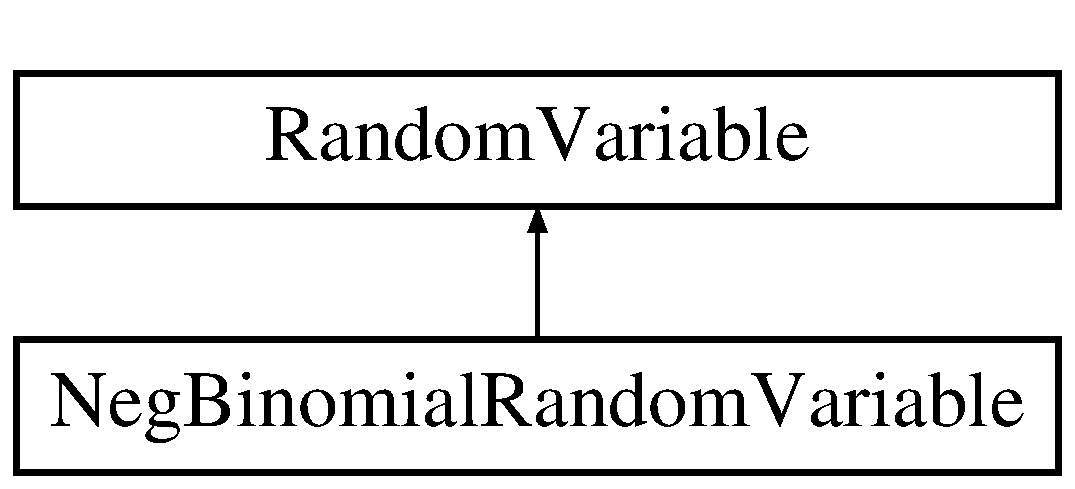
\includegraphics[height=2.000000cm]{classPecos_1_1NegBinomialRandomVariable}
\end{center}
\end{figure}
\subsection*{Public Member Functions}
\begin{DoxyCompactItemize}
\item 
\hyperlink{classPecos_1_1NegBinomialRandomVariable_ad316e61ae4871f5e06b10612ab0d47e6}{Neg\+Binomial\+Random\+Variable} ()\label{classPecos_1_1NegBinomialRandomVariable_ad316e61ae4871f5e06b10612ab0d47e6}

\begin{DoxyCompactList}\small\item\em default constructor \end{DoxyCompactList}\item 
\hyperlink{classPecos_1_1NegBinomialRandomVariable_a4f9bdbb72070afdf5347238f29340c28}{Neg\+Binomial\+Random\+Variable} (unsigned int num\+\_\+trials, Real prob\+\_\+per\+\_\+trial)\label{classPecos_1_1NegBinomialRandomVariable_a4f9bdbb72070afdf5347238f29340c28}

\begin{DoxyCompactList}\small\item\em alternate constructor \end{DoxyCompactList}\item 
\hyperlink{classPecos_1_1NegBinomialRandomVariable_ae28e9edc07dedaa7c2a257fe32bc06ba}{$\sim$\+Neg\+Binomial\+Random\+Variable} ()\label{classPecos_1_1NegBinomialRandomVariable_ae28e9edc07dedaa7c2a257fe32bc06ba}

\begin{DoxyCompactList}\small\item\em destructor \end{DoxyCompactList}\item 
Real \hyperlink{classPecos_1_1NegBinomialRandomVariable_addd564e7f4f314e12d38df74d845f0d8}{cdf} (Real x) const \label{classPecos_1_1NegBinomialRandomVariable_addd564e7f4f314e12d38df74d845f0d8}

\begin{DoxyCompactList}\small\item\em return the cumulative distribution function value of the random variable at x \end{DoxyCompactList}\item 
Real \hyperlink{classPecos_1_1NegBinomialRandomVariable_a23c3b599e7e4788a9a5e9e93c3dbaf4d}{ccdf} (Real x) const \label{classPecos_1_1NegBinomialRandomVariable_a23c3b599e7e4788a9a5e9e93c3dbaf4d}

\begin{DoxyCompactList}\small\item\em return the complementary cumulative distribution function value of the random variable at x \end{DoxyCompactList}\item 
Real \hyperlink{classPecos_1_1NegBinomialRandomVariable_a918a1aac05ca349ea5313eebcba46c3e}{inverse\+\_\+cdf} (Real p\+\_\+cdf) const \label{classPecos_1_1NegBinomialRandomVariable_a918a1aac05ca349ea5313eebcba46c3e}

\begin{DoxyCompactList}\small\item\em return the x value corresponding to a cumulative probability \end{DoxyCompactList}\item 
Real \hyperlink{classPecos_1_1NegBinomialRandomVariable_afda003a1f59ff6930902cd5c8601f49b}{inverse\+\_\+ccdf} (Real p\+\_\+ccdf) const \label{classPecos_1_1NegBinomialRandomVariable_afda003a1f59ff6930902cd5c8601f49b}

\begin{DoxyCompactList}\small\item\em return the x value corresponding to a complementary cumulative probability \end{DoxyCompactList}\item 
Real \hyperlink{classPecos_1_1NegBinomialRandomVariable_a8ec69265f428e17c1707133cb137a819}{pdf} (Real x) const \label{classPecos_1_1NegBinomialRandomVariable_a8ec69265f428e17c1707133cb137a819}

\begin{DoxyCompactList}\small\item\em return the value of the random variable\textquotesingle{}s probability density function at x \end{DoxyCompactList}\item 
Real \hyperlink{classPecos_1_1NegBinomialRandomVariable_aa891dab1ae9a225f493e3a0e5032b778}{parameter} (short dist\+\_\+param) const \label{classPecos_1_1NegBinomialRandomVariable_aa891dab1ae9a225f493e3a0e5032b778}

\begin{DoxyCompactList}\small\item\em return the value of the named distribution parameter \end{DoxyCompactList}\item 
void \hyperlink{classPecos_1_1NegBinomialRandomVariable_ae8e123224f588aee676d5d56d5ca900d}{parameter} (short dist\+\_\+param, Real val)\label{classPecos_1_1NegBinomialRandomVariable_ae8e123224f588aee676d5d56d5ca900d}

\begin{DoxyCompactList}\small\item\em update the value of the named distribution parameter \end{DoxyCompactList}\item 
Real \hyperlink{classPecos_1_1NegBinomialRandomVariable_a962ffe5a3593be370d5c883365c060f4}{mean} () const \label{classPecos_1_1NegBinomialRandomVariable_a962ffe5a3593be370d5c883365c060f4}

\begin{DoxyCompactList}\small\item\em return the distribution mean \end{DoxyCompactList}\item 
Real \hyperlink{classPecos_1_1NegBinomialRandomVariable_ae1fff19ce29a79d657043a598523635d}{median} () const \label{classPecos_1_1NegBinomialRandomVariable_ae1fff19ce29a79d657043a598523635d}

\begin{DoxyCompactList}\small\item\em return the distribution mode \end{DoxyCompactList}\item 
Real \hyperlink{classPecos_1_1NegBinomialRandomVariable_a72d3d6926edd929cb3f8e12baa655f70}{mode} () const \label{classPecos_1_1NegBinomialRandomVariable_a72d3d6926edd929cb3f8e12baa655f70}

\begin{DoxyCompactList}\small\item\em return the distribution mode \end{DoxyCompactList}\item 
Real \hyperlink{classPecos_1_1NegBinomialRandomVariable_a6a4ed9624d511f8a4e4f509c82cb0706}{standard\+\_\+deviation} () const \label{classPecos_1_1NegBinomialRandomVariable_a6a4ed9624d511f8a4e4f509c82cb0706}

\begin{DoxyCompactList}\small\item\em return the distribution variance \end{DoxyCompactList}\item 
Real \hyperlink{classPecos_1_1NegBinomialRandomVariable_a4b8b05b2a9af92dad9cc304c2925a4eb}{variance} () const \label{classPecos_1_1NegBinomialRandomVariable_a4b8b05b2a9af92dad9cc304c2925a4eb}

\begin{DoxyCompactList}\small\item\em return the distribution variance \end{DoxyCompactList}\item 
Real\+Real\+Pair \hyperlink{classPecos_1_1NegBinomialRandomVariable_a4bdb95a8fa5fffaa0de5102f56963cf2}{bounds} () const \label{classPecos_1_1NegBinomialRandomVariable_a4bdb95a8fa5fffaa0de5102f56963cf2}

\begin{DoxyCompactList}\small\item\em return the distribution lower and upper bounds as a pair \end{DoxyCompactList}\item 
void {\bfseries update} (unsigned int num\+\_\+trials, Real prob\+\_\+per\+\_\+trial)\label{classPecos_1_1NegBinomialRandomVariable_a87163ad5a4f469108f079d0e8c6c2cb8}

\end{DoxyCompactItemize}
\subsection*{Static Public Member Functions}
\begin{DoxyCompactItemize}
\item 
static Real {\bfseries pdf} (Real x, unsigned int num\+\_\+trials, Real prob\+\_\+per\+\_\+trial)\label{classPecos_1_1NegBinomialRandomVariable_a2886ea0e23e30bbbc464565416eb6614}

\item 
static Real {\bfseries cdf} (Real x, unsigned int num\+\_\+trials, Real prob\+\_\+per\+\_\+trial)\label{classPecos_1_1NegBinomialRandomVariable_a630e535fde694c4b082312a4fd082f3d}

\item 
static void {\bfseries moments\+\_\+from\+\_\+params} (unsigned int num\+\_\+trials, Real prob\+\_\+per\+\_\+trial, Real \&\hyperlink{classPecos_1_1NegBinomialRandomVariable_a962ffe5a3593be370d5c883365c060f4}{mean}, Real \&std\+\_\+dev)\label{classPecos_1_1NegBinomialRandomVariable_ab5304d2842c683e30818638d9e7150ba}

\end{DoxyCompactItemize}
\subsection*{Protected Member Functions}
\begin{DoxyCompactItemize}
\item 
void \hyperlink{classPecos_1_1NegBinomialRandomVariable_aaa6750cbee2245416a6eeeac58d4405a}{update\+\_\+boost} ()\label{classPecos_1_1NegBinomialRandomVariable_aaa6750cbee2245416a6eeeac58d4405a}

\begin{DoxyCompactList}\small\item\em create a new neg\+Binomial\+Dist instance \end{DoxyCompactList}\end{DoxyCompactItemize}
\subsection*{Protected Attributes}
\begin{DoxyCompactItemize}
\item 
unsigned int \hyperlink{classPecos_1_1NegBinomialRandomVariable_ae7284c5049f25d6872f8fbe98c855e0c}{num\+Trials}\label{classPecos_1_1NegBinomialRandomVariable_ae7284c5049f25d6872f8fbe98c855e0c}

\begin{DoxyCompactList}\small\item\em r parameter of negative binomial random variable \end{DoxyCompactList}\item 
Real \hyperlink{classPecos_1_1NegBinomialRandomVariable_a034cce918fd6c1433e74212387527794}{prob\+Per\+Trial}\label{classPecos_1_1NegBinomialRandomVariable_a034cce918fd6c1433e74212387527794}

\begin{DoxyCompactList}\small\item\em p parameter of negative binomial random variable \end{DoxyCompactList}\item 
negative\+\_\+binomial\+\_\+dist $\ast$ \hyperlink{classPecos_1_1NegBinomialRandomVariable_a11407882148ec2a21c271c5001db9f4d}{neg\+Binomial\+Dist}\label{classPecos_1_1NegBinomialRandomVariable_a11407882148ec2a21c271c5001db9f4d}

\begin{DoxyCompactList}\small\item\em pointer to the Boost negative\+\_\+binomial\+\_\+distribution instance \end{DoxyCompactList}\end{DoxyCompactItemize}


\subsection{Detailed Description}
Derived random variable class for negative binomial random variables. 

Manages num\+Trials and prob\+Per\+Trial parameters. Note that the geometric distribution is a special case of the negative binomial distribution for num\+Trials = 1; however, there is currently little benefit to deriving \hyperlink{classPecos_1_1NegBinomialRandomVariable}{Neg\+Binomial\+Random\+Variable} from \hyperlink{classPecos_1_1GeometricRandomVariable}{Geometric\+Random\+Variable} (e.\+g., the Boost distribution pointers are distinct). 

The documentation for this class was generated from the following file\+:\begin{DoxyCompactItemize}
\item 
Neg\+Binomial\+Random\+Variable.\+hpp\end{DoxyCompactItemize}

\section{Nodal\+Interp\+Poly\+Approximation Class Reference}
\label{classPecos_1_1NodalInterpPolyApproximation}\index{Nodal\+Interp\+Poly\+Approximation@{Nodal\+Interp\+Poly\+Approximation}}


Derived approximation class for nodal interpolation polynomials (global approximation interpolating function values and potentially gradients at collocation points).  


Inheritance diagram for Nodal\+Interp\+Poly\+Approximation\+:\begin{figure}[H]
\begin{center}
\leavevmode
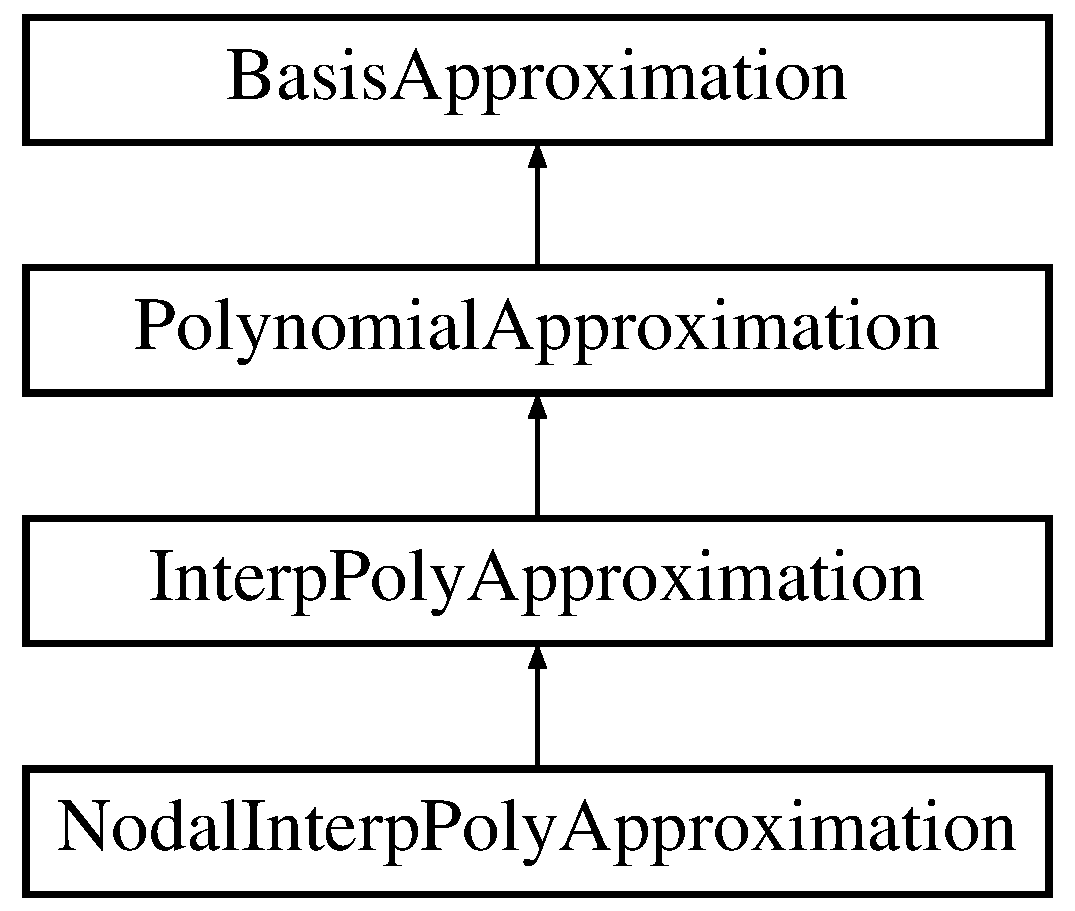
\includegraphics[height=4.000000cm]{classPecos_1_1NodalInterpPolyApproximation}
\end{center}
\end{figure}
\subsection*{Public Member Functions}
\begin{DoxyCompactItemize}
\item 
\hyperlink{classPecos_1_1NodalInterpPolyApproximation_ab62435d42ec6181d9184a90a9fc2032f}{Nodal\+Interp\+Poly\+Approximation} (const \hyperlink{classPecos_1_1SharedBasisApproxData}{Shared\+Basis\+Approx\+Data} \&shared\+\_\+data)\label{classPecos_1_1NodalInterpPolyApproximation_ab62435d42ec6181d9184a90a9fc2032f}

\begin{DoxyCompactList}\small\item\em default constructor \end{DoxyCompactList}\item 
\hyperlink{classPecos_1_1NodalInterpPolyApproximation_a2edcc80dff98544e7e3de4a5c35e3e97}{$\sim$\+Nodal\+Interp\+Poly\+Approximation} ()\label{classPecos_1_1NodalInterpPolyApproximation_a2edcc80dff98544e7e3de4a5c35e3e97}

\begin{DoxyCompactList}\small\item\em destructor \end{DoxyCompactList}\end{DoxyCompactItemize}
\subsection*{Protected Member Functions}
\begin{DoxyCompactItemize}
\item 
void \hyperlink{classPecos_1_1NodalInterpPolyApproximation_a37ef37829b412fefa40d53b395846781}{allocate\+\_\+arrays} ()\label{classPecos_1_1NodalInterpPolyApproximation_a37ef37829b412fefa40d53b395846781}

\begin{DoxyCompactList}\small\item\em size expansion\+Type\{1,2\}Coeffs and expansion\+Type1\+Coeff\+Grads \end{DoxyCompactList}\item 
void \hyperlink{classPecos_1_1NodalInterpPolyApproximation_aef8f0c32bdeff7756a9c614607c03058}{compute\+\_\+coefficients} (size\+\_\+t index=\+\_\+\+N\+P\+OS)\label{classPecos_1_1NodalInterpPolyApproximation_aef8f0c32bdeff7756a9c614607c03058}

\begin{DoxyCompactList}\small\item\em calculate the approximation coefficients using a set of surrogate data \end{DoxyCompactList}\item 
void \hyperlink{classPecos_1_1NodalInterpPolyApproximation_a8ba12605934048176c1d1c5722465523}{increment\+\_\+coefficients} (size\+\_\+t index=\+\_\+\+N\+P\+OS)\label{classPecos_1_1NodalInterpPolyApproximation_a8ba12605934048176c1d1c5722465523}

\begin{DoxyCompactList}\small\item\em update the coefficients for the expansion of interpolation polynomials\+: increment expansion\{Type1\+Coeffs,Type2\+Coeffs,Type1\+Coeff\+Grads\} \end{DoxyCompactList}\item 
void \hyperlink{classPecos_1_1NodalInterpPolyApproximation_a662fd880fee0ed53f1e3383c41d6b792}{decrement\+\_\+coefficients} (bool save\+\_\+data)\label{classPecos_1_1NodalInterpPolyApproximation_a662fd880fee0ed53f1e3383c41d6b792}

\begin{DoxyCompactList}\small\item\em restore the coefficients to their previous state prior to last increment\+: decrement expansion\{Type1\+Coeffs,Type2\+Coeffs,Type1\+Coeff\+Grads\} \end{DoxyCompactList}\item 
void \hyperlink{classPecos_1_1NodalInterpPolyApproximation_a150c32326f6c12d2303806005715706e}{push\+\_\+coefficients} ()\label{classPecos_1_1NodalInterpPolyApproximation_a150c32326f6c12d2303806005715706e}

\begin{DoxyCompactList}\small\item\em restore the coefficients to a previously incremented state as identified by the current increment to the Smolyak multi index\+: push expansion\{Type1\+Coeffs,Type2\+Coeffs,Type1\+Coeff\+Grads\} \end{DoxyCompactList}\item 
void \hyperlink{classPecos_1_1NodalInterpPolyApproximation_a742e0217d6f681e08f401409771f4f4a}{finalize\+\_\+coefficients} ()\label{classPecos_1_1NodalInterpPolyApproximation_a742e0217d6f681e08f401409771f4f4a}

\begin{DoxyCompactList}\small\item\em finalize the coefficients by applying all previously evaluated increments\+: finalize expansion\{Type1\+Coeffs,Type2\+Coeffs,Type1\+Coeff\+Grads\} \end{DoxyCompactList}\item 
void \hyperlink{classPecos_1_1NodalInterpPolyApproximation_abc17a7104c33d8146f4a0ee7b6c6f37a}{store\+\_\+coefficients} (size\+\_\+t index=\+\_\+\+N\+P\+OS)\label{classPecos_1_1NodalInterpPolyApproximation_abc17a7104c33d8146f4a0ee7b6c6f37a}

\begin{DoxyCompactList}\small\item\em store current state within stored\+Exp\+Type\{1\+Coeffs,2\+Coeffs,1\+Coeff\+Grads\} \end{DoxyCompactList}\item 
void \hyperlink{classPecos_1_1NodalInterpPolyApproximation_ad05b093ee96314c9e05bad8e06c2dae7}{restore\+\_\+coefficients} (size\+\_\+t index=\+\_\+\+N\+P\+OS)\label{classPecos_1_1NodalInterpPolyApproximation_ad05b093ee96314c9e05bad8e06c2dae7}

\begin{DoxyCompactList}\small\item\em restore previous state from stored\+Exp\+Type\{1\+Coeffs,2\+Coeffs,1\+Coeff\+Grads\} \end{DoxyCompactList}\item 
void \hyperlink{classPecos_1_1NodalInterpPolyApproximation_af5c6af74d2c8c5575fefb46ce55af90d}{swap\+\_\+coefficients} (size\+\_\+t index)\label{classPecos_1_1NodalInterpPolyApproximation_af5c6af74d2c8c5575fefb46ce55af90d}

\begin{DoxyCompactList}\small\item\em swap stored\+Exp\+Type\{1\+Coeffs,2\+Coeffs,1\+Coeff\+Grads\}\mbox{[}index\mbox{]} with active current data \end{DoxyCompactList}\item 
void \hyperlink{classPecos_1_1NodalInterpPolyApproximation_a63d12cc6021fda4896b8738d72dfcc86}{remove\+\_\+stored\+\_\+coefficients} (size\+\_\+t index=\+\_\+\+N\+P\+OS)\label{classPecos_1_1NodalInterpPolyApproximation_a63d12cc6021fda4896b8738d72dfcc86}

\begin{DoxyCompactList}\small\item\em remove a redundant entry from stored\+Exp\+Type\{1\+Coeffs,2\+Coeffs,1\+Coeff\+Grads\} prior to combine\+\_\+coefficients (default is pop\+\_\+back) \end{DoxyCompactList}\item 
void \hyperlink{classPecos_1_1NodalInterpPolyApproximation_ae4337960917eda26a5672e5c6afbb62a}{clear\+\_\+stored} ()\label{classPecos_1_1NodalInterpPolyApproximation_ae4337960917eda26a5672e5c6afbb62a}

\begin{DoxyCompactList}\small\item\em clear stored\+Exp\+Type\{1\+Coeffs,2\+Coeffs,1\+Coeff\+Grads\} \end{DoxyCompactList}\item 
void \hyperlink{classPecos_1_1NodalInterpPolyApproximation_a7c794213befc83c9f90137f22e4cd39d}{combine\+\_\+coefficients} (size\+\_\+t swap\+\_\+index)\label{classPecos_1_1NodalInterpPolyApproximation_a7c794213befc83c9f90137f22e4cd39d}

\begin{DoxyCompactList}\small\item\em augment current interpolant using stored\+Exp\+Type\{1\+Coeffs,2\+Coeffs,1\+Coeff\+Grads\}\mbox{[}index\mbox{]} \end{DoxyCompactList}\item 
void \hyperlink{classPecos_1_1NodalInterpPolyApproximation_a9e2f6de3dafca8df624fef2a132b5185}{integrate\+\_\+response\+\_\+moments} (size\+\_\+t num\+\_\+moments)\label{classPecos_1_1NodalInterpPolyApproximation_a9e2f6de3dafca8df624fef2a132b5185}

\begin{DoxyCompactList}\small\item\em compute moments of response using numerical integration \end{DoxyCompactList}\item 
void \hyperlink{classPecos_1_1NodalInterpPolyApproximation_a611ac6de1665bc1197922b77823250c2}{integrate\+\_\+expansion\+\_\+moments} (size\+\_\+t num\+\_\+moments)\label{classPecos_1_1NodalInterpPolyApproximation_a611ac6de1665bc1197922b77823250c2}

\begin{DoxyCompactList}\small\item\em compute moments of expansion using numerical integration \end{DoxyCompactList}\item 
Real \hyperlink{classPecos_1_1NodalInterpPolyApproximation_a7bc9dcdf32fc46f97e286268c1ac51b0}{value} (const Real\+Vector \&x)\label{classPecos_1_1NodalInterpPolyApproximation_a7bc9dcdf32fc46f97e286268c1ac51b0}

\begin{DoxyCompactList}\small\item\em retrieve the approximate function value for a given parameter vector \end{DoxyCompactList}\item 
const Real\+Vector \& \hyperlink{classPecos_1_1NodalInterpPolyApproximation_ae3b6ea541392b74cf0cc8758e206277c}{gradient\+\_\+basis\+\_\+variables} (const Real\+Vector \&x)\label{classPecos_1_1NodalInterpPolyApproximation_ae3b6ea541392b74cf0cc8758e206277c}

\begin{DoxyCompactList}\small\item\em retrieve the gradient for a response expansion with respect to all variables included in the polynomial bases using the given parameter vector and default D\+VV \end{DoxyCompactList}\item 
const Real\+Vector \& \hyperlink{classPecos_1_1NodalInterpPolyApproximation_a3ffb563ae1658344bfc2ad882def9e7c}{gradient\+\_\+basis\+\_\+variables} (const Real\+Vector \&x, const Sizet\+Array \&dvv)
\item 
const Real\+Vector \& \hyperlink{classPecos_1_1NodalInterpPolyApproximation_a518e8604f973a4b161a9b5718a0aa25e}{gradient\+\_\+nonbasis\+\_\+variables} (const Real\+Vector \&x)\label{classPecos_1_1NodalInterpPolyApproximation_a518e8604f973a4b161a9b5718a0aa25e}

\begin{DoxyCompactList}\small\item\em retrieve the gradient for a response expansion with respect to all variables not included in the polynomial bases (nonprobabilistic variables such as design or epistemic when not in \char`\"{}all\char`\"{} mode) using the given parameter vector and default D\+VV \end{DoxyCompactList}\item 
const Real\+Sym\+Matrix \& \hyperlink{classPecos_1_1NodalInterpPolyApproximation_a830729654265d84af637960f8c63f2bc}{hessian\+\_\+basis\+\_\+variables} (const Real\+Vector \&x)\label{classPecos_1_1NodalInterpPolyApproximation_a830729654265d84af637960f8c63f2bc}

\begin{DoxyCompactList}\small\item\em retrieve the Hessian of the response expansion with respect to all variables included in the polynomial basis (e.\+g., probabilistic variables) for a given parameter vector \end{DoxyCompactList}\item 
Real \hyperlink{classPecos_1_1NodalInterpPolyApproximation_a1abe918dbdc66ac0fde85f1ab3c061af}{stored\+\_\+value} (const Real\+Vector \&x, size\+\_\+t index)\label{classPecos_1_1NodalInterpPolyApproximation_a1abe918dbdc66ac0fde85f1ab3c061af}

\begin{DoxyCompactList}\small\item\em retrieve the response value for a stored expansion using the given parameter vector \end{DoxyCompactList}\item 
const Real\+Vector \& \hyperlink{classPecos_1_1NodalInterpPolyApproximation_a7689fc058e2efdde6ce4dfe898864592}{stored\+\_\+gradient\+\_\+basis\+\_\+variables} (const Real\+Vector \&x, size\+\_\+t index)\label{classPecos_1_1NodalInterpPolyApproximation_a7689fc058e2efdde6ce4dfe898864592}

\begin{DoxyCompactList}\small\item\em retrieve the response gradient for a stored expansion with respect to all variables included in the polynomial bases; evaluate for the given parameter vector. \end{DoxyCompactList}\item 
const Real\+Vector \& \hyperlink{classPecos_1_1NodalInterpPolyApproximation_af0c9184d9a0da7b0e3d0d3ecbfc8f434}{stored\+\_\+gradient\+\_\+nonbasis\+\_\+variables} (const Real\+Vector \&x, size\+\_\+t index)\label{classPecos_1_1NodalInterpPolyApproximation_af0c9184d9a0da7b0e3d0d3ecbfc8f434}

\begin{DoxyCompactList}\small\item\em retrieve the response gradient for a stored expansion with respect to all variables not included in the polynomial bases; evaluate for the given parameter vector. \end{DoxyCompactList}\item 
Real \hyperlink{classPecos_1_1NodalInterpPolyApproximation_adc6f262952d05a33ff68cae37929cbb2}{mean} ()
\item 
Real \hyperlink{classPecos_1_1NodalInterpPolyApproximation_aed107df248a4555c052446fbc10a8e61}{mean} (const Real\+Vector \&x)
\item 
const Real\+Vector \& \hyperlink{classPecos_1_1NodalInterpPolyApproximation_a069c87a26fdb4b09af68db26abd646a0}{mean\+\_\+gradient} ()
\item 
const Real\+Vector \& \hyperlink{classPecos_1_1NodalInterpPolyApproximation_a24f2edc21c9887121cda78faae1c1475}{mean\+\_\+gradient} (const Real\+Vector \&x, const Sizet\+Array \&dvv)
\item 
Real \hyperlink{classPecos_1_1NodalInterpPolyApproximation_a38f6da77468be17e02ce38af2c0976c3}{variance} ()
\item 
Real \hyperlink{classPecos_1_1NodalInterpPolyApproximation_acbdcb523a161d7d3a5cc190796e84ede}{variance} (const Real\+Vector \&x)
\item 
const Real\+Vector \& \hyperlink{classPecos_1_1NodalInterpPolyApproximation_ae898fc2f42f1077268f89fc2e9f2c71c}{variance\+\_\+gradient} ()
\item 
const Real\+Vector \& \hyperlink{classPecos_1_1NodalInterpPolyApproximation_a791e127a445f8a6c9c3a7966d12c1431}{variance\+\_\+gradient} (const Real\+Vector \&x, const Sizet\+Array \&dvv)
\item 
Real \hyperlink{classPecos_1_1NodalInterpPolyApproximation_ac0085912d4abb9caa3f480b9c6778c0e}{covariance} (\hyperlink{classPecos_1_1PolynomialApproximation}{Polynomial\+Approximation} $\ast$poly\+\_\+approx\+\_\+2)
\item 
Real \hyperlink{classPecos_1_1NodalInterpPolyApproximation_afc1731a3d89818d49c03a3c20a7a2898}{covariance} (const Real\+Vector \&x, \hyperlink{classPecos_1_1PolynomialApproximation}{Polynomial\+Approximation} $\ast$poly\+\_\+approx\+\_\+2)
\item 
void {\bfseries compute\+\_\+total\+\_\+sobol\+\_\+indices} ()\label{classPecos_1_1NodalInterpPolyApproximation_a9b445d773d12ed85eb56bb73f6d7e540}

\item 
void \hyperlink{classPecos_1_1NodalInterpPolyApproximation_a6eb2548a8c786f48478fabb6377be779}{compute\+\_\+partial\+\_\+variance} (const Bit\+Array \&set\+\_\+value)
\item 
Real\+Vector \hyperlink{classPecos_1_1NodalInterpPolyApproximation_ac64f16ff9fbfb80c4bafa969b4a92e1d}{approximation\+\_\+coefficients} (bool normalized) const \label{classPecos_1_1NodalInterpPolyApproximation_ac64f16ff9fbfb80c4bafa969b4a92e1d}

\begin{DoxyCompactList}\small\item\em return the coefficient array computed by \hyperlink{classPecos_1_1NodalInterpPolyApproximation_aef8f0c32bdeff7756a9c614607c03058}{compute\+\_\+coefficients()} \end{DoxyCompactList}\item 
void \hyperlink{classPecos_1_1NodalInterpPolyApproximation_a2e7b82322962df3fd036b9e0783d8fc9}{approximation\+\_\+coefficients} (const Real\+Vector \&approx\+\_\+coeffs, bool normalized)\label{classPecos_1_1NodalInterpPolyApproximation_a2e7b82322962df3fd036b9e0783d8fc9}

\begin{DoxyCompactList}\small\item\em set the coefficient array from external sources, rather than computing with \hyperlink{classPecos_1_1NodalInterpPolyApproximation_aef8f0c32bdeff7756a9c614607c03058}{compute\+\_\+coefficients()} \end{DoxyCompactList}\end{DoxyCompactItemize}
\subsection*{Private Member Functions}
\begin{DoxyCompactItemize}
\item 
void \hyperlink{classPecos_1_1NodalInterpPolyApproximation_a462bc6aefbe884d10284098edb819534}{update\+\_\+expansion\+\_\+coefficients} ()\label{classPecos_1_1NodalInterpPolyApproximation_a462bc6aefbe884d10284098edb819534}

\begin{DoxyCompactList}\small\item\em update expansion\+Type\{1\+Coeffs,2\+Coeffs,1\+Coeff\+Grads\} following changes to surr\+Data \end{DoxyCompactList}\item 
Real \hyperlink{classPecos_1_1NodalInterpPolyApproximation_a688440d598a119d9b059aa0199886c75}{tensor\+\_\+product\+\_\+mean} (const Real\+Vector \&x, const U\+Short\+Array \&lev\+\_\+index, const U\+Short2\+D\+Array \&key, const Sizet\+Array \&colloc\+\_\+index)
\begin{DoxyCompactList}\small\item\em compute the mean of a tensor interpolant on a tensor grid; contributes to mean(x) \end{DoxyCompactList}\item 
const Real\+Vector \& \hyperlink{classPecos_1_1NodalInterpPolyApproximation_ac8b724a720250bb907f8828b3d2f6979}{tensor\+\_\+product\+\_\+mean\+\_\+gradient} (const Real\+Vector \&x, const U\+Short\+Array \&lev\+\_\+index, const U\+Short2\+D\+Array \&key, const Sizet\+Array \&colloc\+\_\+index, const Sizet\+Array \&dvv)
\begin{DoxyCompactList}\small\item\em compute the gradient of the mean of a tensor interpolant on a tensor grid; contributes to mean\+\_\+gradient(x) \end{DoxyCompactList}\item 
Real \hyperlink{classPecos_1_1NodalInterpPolyApproximation_ad34fcf2d6c6841648fa93e0e8e6bef78}{tensor\+\_\+product\+\_\+covariance} (const Real\+Vector \&x, const U\+Short\+Array \&lev\+\_\+index, const U\+Short2\+D\+Array \&key, const Sizet\+Array \&colloc\+\_\+index, \hyperlink{classPecos_1_1NodalInterpPolyApproximation}{Nodal\+Interp\+Poly\+Approximation} $\ast$nip\+\_\+approx\+\_\+2)
\begin{DoxyCompactList}\small\item\em compute the covariance of two tensor interpolants on the same tensor grid using an interpolation of products or product of interpolants approach; contributes to covariance(x, poly\+\_\+approx\+\_\+2) \end{DoxyCompactList}\item 
Real \hyperlink{classPecos_1_1NodalInterpPolyApproximation_a4f0ee291e5061aedbbd6930aa607ead7}{tensor\+\_\+product\+\_\+covariance} (const Real\+Vector \&x, const U\+Short\+Array \&lev\+\_\+index\+\_\+1, const U\+Short2\+D\+Array \&key\+\_\+1, const Sizet\+Array \&colloc\+\_\+index\+\_\+1, const U\+Short\+Array \&lev\+\_\+index\+\_\+2, const U\+Short2\+D\+Array \&key\+\_\+2, const Sizet\+Array \&colloc\+\_\+index\+\_\+2, \hyperlink{classPecos_1_1NodalInterpPolyApproximation}{Nodal\+Interp\+Poly\+Approximation} $\ast$nip\+\_\+approx\+\_\+2)
\begin{DoxyCompactList}\small\item\em compute the covariance of two tensor interpolants on different tensor grids using a product of interpolants approach; contributes to covariance(x, poly\+\_\+approx\+\_\+2) \end{DoxyCompactList}\item 
const Real\+Vector \& \hyperlink{classPecos_1_1NodalInterpPolyApproximation_a2e321deaf54c63212ba2d926aa0ad08d}{tensor\+\_\+product\+\_\+variance\+\_\+gradient} (const Real\+Vector \&x, const U\+Short\+Array \&lev\+\_\+index, const U\+Short2\+D\+Array \&key, const Sizet\+Array \&colloc\+\_\+index, const Sizet\+Array \&dvv)
\begin{DoxyCompactList}\small\item\em compute the gradient of the variance of a tensor interpolant on a tensor grid using an interpolation of products or product of interpolants approach; contributes to variance\+\_\+gradient(x) \end{DoxyCompactList}\item 
Real \hyperlink{classPecos_1_1NodalInterpPolyApproximation_add4c66b2a8fb14693ad22751f7526b84}{value} (const Real\+Vector \&x, const Real\+Vector\+Array \&t1\+\_\+coeffs, const Real\+Matrix\+Array \&t2\+\_\+coeffs, const U\+Short3\+D\+Array \&colloc\+\_\+key, const Sizet\+List \&subset\+\_\+indices)
\begin{DoxyCompactList}\small\item\em compute value of reduced-\/dimension interpolant \end{DoxyCompactList}\item 
const Real\+Vector \& \hyperlink{classPecos_1_1NodalInterpPolyApproximation_ab95fcef1d7128a740285b8a8ce9071e4}{gradient\+\_\+basis\+\_\+variables} (const Real\+Vector \&x, const Real\+Vector\+Array \&t1\+\_\+coeffs, const Real\+Matrix\+Array \&t2\+\_\+coeffs, const U\+Short3\+D\+Array \&colloc\+\_\+key, const Sizet\+List \&subset\+\_\+indices)\label{classPecos_1_1NodalInterpPolyApproximation_ab95fcef1d7128a740285b8a8ce9071e4}

\begin{DoxyCompactList}\small\item\em compute gradient of reduced-\/dimension interpolant with respect to basis variables \end{DoxyCompactList}\item 
Real \hyperlink{classPecos_1_1NodalInterpPolyApproximation_a4057786fc84fcd04ea07744a0a928b4a}{expectation} (const Real\+Vector \&t1\+\_\+coeffs, const Real\+Matrix \&t2\+\_\+coeffs)\label{classPecos_1_1NodalInterpPolyApproximation_a4057786fc84fcd04ea07744a0a928b4a}

\begin{DoxyCompactList}\small\item\em compute the expected value of the interpolant given by t\{1,2\}\+\_\+coeffs using weights from the \hyperlink{classPecos_1_1CombinedSparseGridDriver}{Combined\+Sparse\+Grid\+Driver} \end{DoxyCompactList}\item 
Real \hyperlink{classPecos_1_1NodalInterpPolyApproximation_ae0468e01d194de5eeecc306be0e9ab4e}{expectation} (const Real\+Vector \&t1\+\_\+coeffs, const Real\+Vector \&t1\+\_\+wts, const Real\+Matrix \&t2\+\_\+coeffs, const Real\+Matrix \&t2\+\_\+wts)\label{classPecos_1_1NodalInterpPolyApproximation_ae0468e01d194de5eeecc306be0e9ab4e}

\begin{DoxyCompactList}\small\item\em compute the expected value of the interpolant given by t\{1,2\}\+\_\+coeffs using t\{1,2\}\+\_\+wts \end{DoxyCompactList}\item 
void \hyperlink{classPecos_1_1NodalInterpPolyApproximation_ae4a694a92e56149b20cf5b7450d3518a}{reinterpolated\+\_\+level} (const U\+Short\+Array \&lev\+\_\+index)
\begin{DoxyCompactList}\small\item\em computes higher-\/order grid for tensor reinterpolation of the covariance fn for non-\/integrated dimensions in all\+\_\+variables mode \end{DoxyCompactList}\item 
Real \hyperlink{classPecos_1_1NodalInterpPolyApproximation_acabcaa681df99b0bb8f2daed023abc1b}{member\+\_\+integral} (const Bit\+Array \&member\+\_\+bits, Real \hyperlink{classPecos_1_1NodalInterpPolyApproximation_adc6f262952d05a33ff68cae37929cbb2}{mean})
\begin{DoxyCompactList}\small\item\em compute integral for total Sobol\textquotesingle{} index for variables in a set \end{DoxyCompactList}\item 
void \hyperlink{classPecos_1_1NodalInterpPolyApproximation_a141b7db5079aa372a5f8727ea856679e}{member\+\_\+coefficients\+\_\+weights} (const Bit\+Array \&member\+\_\+bits, const U\+Short\+Array \&quad\+\_\+order, const U\+Short\+Array \&lev\+\_\+index, const U\+Short2\+D\+Array \&colloc\+\_\+key, const Sizet\+Array \&colloc\+\_\+index, Real\+Vector \&member\+\_\+t1\+\_\+coeffs, Real\+Vector \&member\+\_\+t1\+\_\+wts, Real\+Matrix \&member\+\_\+t2\+\_\+coeffs, Real\+Matrix \&member\+\_\+t2\+\_\+wts, U\+Short2\+D\+Array \&member\+\_\+colloc\+\_\+key, Sizet\+Array \&member\+\_\+colloc\+\_\+index)\label{classPecos_1_1NodalInterpPolyApproximation_a141b7db5079aa372a5f8727ea856679e}

\begin{DoxyCompactList}\small\item\em defines member\+\_\+coeffs and member\+\_\+wts for a particular membership set \end{DoxyCompactList}\item 
void \hyperlink{classPecos_1_1NodalInterpPolyApproximation_acc8e046d91e34a5404891d6bd48aa2d0}{update\+\_\+member\+\_\+key} (const U\+Short\+Array \&data, const Sizet\+List \&member\+\_\+indices, U\+Short\+Array \&member\+\_\+map\+\_\+key, size\+\_\+t cntr)\label{classPecos_1_1NodalInterpPolyApproximation_acc8e046d91e34a5404891d6bd48aa2d0}

\begin{DoxyCompactList}\small\item\em create a unique map key for \hyperlink{classPecos_1_1NodalInterpPolyApproximation_a7bc9dcdf32fc46f97e286268c1ac51b0}{value()} and \hyperlink{classPecos_1_1PolynomialApproximation_a42bf374bf23c32c941ee2acae5ad56a4}{gradient()} calculation reuse \end{DoxyCompactList}\end{DoxyCompactItemize}
\subsection*{Private Attributes}
\begin{DoxyCompactItemize}
\item 
Real\+Vector \hyperlink{classPecos_1_1NodalInterpPolyApproximation_ae8d5859e28682d657aecfb767cd45468}{expansion\+Type1\+Coeffs}\label{classPecos_1_1NodalInterpPolyApproximation_ae8d5859e28682d657aecfb767cd45468}

\begin{DoxyCompactList}\small\item\em the type1 coefficients of the expansion for interpolating values \end{DoxyCompactList}\item 
Real\+Matrix \hyperlink{classPecos_1_1NodalInterpPolyApproximation_a869953a9afd97641609b85ae03f016f6}{expansion\+Type2\+Coeffs}\label{classPecos_1_1NodalInterpPolyApproximation_a869953a9afd97641609b85ae03f016f6}

\begin{DoxyCompactList}\small\item\em the type2 coefficients of the expansion for interpolating gradients \end{DoxyCompactList}\item 
Real\+Matrix \hyperlink{classPecos_1_1NodalInterpPolyApproximation_af95aafb683b36750f8e24fb858cbe8b2}{expansion\+Type1\+Coeff\+Grads}
\begin{DoxyCompactList}\small\item\em the gradients of the type1 expansion coefficients \end{DoxyCompactList}\item 
Real\+Vector\+Array \hyperlink{classPecos_1_1NodalInterpPolyApproximation_a26b078979062892ab4016332d295d79f}{stored\+Exp\+Type1\+Coeffs}\label{classPecos_1_1NodalInterpPolyApproximation_a26b078979062892ab4016332d295d79f}

\begin{DoxyCompactList}\small\item\em copies of expansion\+Type1\+Coeffs state for subsequent restoration \end{DoxyCompactList}\item 
Real\+Matrix\+Array \hyperlink{classPecos_1_1NodalInterpPolyApproximation_ab19d3902112d6229965c9e77e1d88cca}{stored\+Exp\+Type2\+Coeffs}\label{classPecos_1_1NodalInterpPolyApproximation_ab19d3902112d6229965c9e77e1d88cca}

\begin{DoxyCompactList}\small\item\em copies of expansion\+Type2\+Coeffs state for subsequent restoration \end{DoxyCompactList}\item 
Real\+Matrix\+Array \hyperlink{classPecos_1_1NodalInterpPolyApproximation_a8dc2b2f98351f6761016c72f97a85757}{stored\+Exp\+Type1\+Coeff\+Grads}\label{classPecos_1_1NodalInterpPolyApproximation_a8dc2b2f98351f6761016c72f97a85757}

\begin{DoxyCompactList}\small\item\em copies of expansion\+Type1\+Coeff\+Grads state for subsequent restoration \end{DoxyCompactList}\item 
Real\+Vector \hyperlink{classPecos_1_1NodalInterpPolyApproximation_abe4e2e7034cc34287a55bc222635c275}{tp\+Mean\+Grad}\label{classPecos_1_1NodalInterpPolyApproximation_abe4e2e7034cc34287a55bc222635c275}

\begin{DoxyCompactList}\small\item\em the gradient of the mean of a tensor-\/product interpolant; a contributor to mean\+Gradient \end{DoxyCompactList}\item 
Real\+Vector \hyperlink{classPecos_1_1NodalInterpPolyApproximation_ae2ca11b7c6367e7601a2c3e6430fe8c0}{tp\+Variance\+Grad}\label{classPecos_1_1NodalInterpPolyApproximation_ae2ca11b7c6367e7601a2c3e6430fe8c0}

\begin{DoxyCompactList}\small\item\em the gradient of the variance of a tensor-\/product interpolant; a contributor to variance\+Gradient \end{DoxyCompactList}\end{DoxyCompactItemize}
\subsection*{Additional Inherited Members}


\subsection{Detailed Description}
Derived approximation class for nodal interpolation polynomials (global approximation interpolating function values and potentially gradients at collocation points). 

The \hyperlink{classPecos_1_1NodalInterpPolyApproximation}{Nodal\+Interp\+Poly\+Approximation} class provides a global polynomial approximation based on either Lagrange or Hermite interpolation polynomials using a nodal basis approach. It is used primarily for stochastic collocation approaches to uncertainty quantification. 

\subsection{Member Function Documentation}
\index{Pecos\+::\+Nodal\+Interp\+Poly\+Approximation@{Pecos\+::\+Nodal\+Interp\+Poly\+Approximation}!gradient\+\_\+basis\+\_\+variables@{gradient\+\_\+basis\+\_\+variables}}
\index{gradient\+\_\+basis\+\_\+variables@{gradient\+\_\+basis\+\_\+variables}!Pecos\+::\+Nodal\+Interp\+Poly\+Approximation@{Pecos\+::\+Nodal\+Interp\+Poly\+Approximation}}
\subsubsection[{\texorpdfstring{gradient\+\_\+basis\+\_\+variables(const Real\+Vector \&x, const Sizet\+Array \&dvv)}{gradient_basis_variables(const RealVector &x, const SizetArray &dvv)}}]{\setlength{\rightskip}{0pt plus 5cm}const Real\+Vector \& gradient\+\_\+basis\+\_\+variables (
\begin{DoxyParamCaption}
\item[{const Real\+Vector \&}]{x, }
\item[{const Sizet\+Array \&}]{dvv}
\end{DoxyParamCaption}
)\hspace{0.3cm}{\ttfamily [protected]}, {\ttfamily [virtual]}}\label{classPecos_1_1NodalInterpPolyApproximation_a3ffb563ae1658344bfc2ad882def9e7c}
Special case used for sparse grid interpolation on variable sub-\/sets defined from partial integration. 

Implements \hyperlink{classPecos_1_1PolynomialApproximation_acbdc4eeec56540a31e44ca2df5414ffd}{Polynomial\+Approximation}.



References Polynomial\+Approximation\+::approx\+Gradient, Combined\+Sparse\+Grid\+Driver\+::collocation\+\_\+indices(), Tensor\+Product\+Driver\+::collocation\+\_\+key(), Combined\+Sparse\+Grid\+Driver\+::collocation\+\_\+key(), Shared\+Nodal\+Interp\+Poly\+Approx\+Data\+::csg\+\_\+driver(), Polynomial\+Approximation\+::expansion\+Coeff\+Flag, Nodal\+Interp\+Poly\+Approximation\+::expansion\+Type1\+Coeffs, Nodal\+Interp\+Poly\+Approximation\+::expansion\+Type2\+Coeffs, Expansion\+Config\+Options\+::exp\+Coeffs\+Soln\+Approach, Shared\+Poly\+Approx\+Data\+::exp\+Config\+Options, Nodal\+Interp\+Poly\+Approximation\+::gradient\+\_\+nonbasis\+\_\+variables(), Tensor\+Product\+Driver\+::level\+\_\+index(), Basis\+Approximation\+::shared\+Data\+Rep, Combined\+Sparse\+Grid\+Driver\+::smolyak\+\_\+coefficients(), Combined\+Sparse\+Grid\+Driver\+::smolyak\+\_\+multi\+\_\+index(), and Shared\+Nodal\+Interp\+Poly\+Approx\+Data\+::tpq\+\_\+driver().

\index{Pecos\+::\+Nodal\+Interp\+Poly\+Approximation@{Pecos\+::\+Nodal\+Interp\+Poly\+Approximation}!mean@{mean}}
\index{mean@{mean}!Pecos\+::\+Nodal\+Interp\+Poly\+Approximation@{Pecos\+::\+Nodal\+Interp\+Poly\+Approximation}}
\subsubsection[{\texorpdfstring{mean()}{mean()}}]{\setlength{\rightskip}{0pt plus 5cm}Real mean (
\begin{DoxyParamCaption}
{}
\end{DoxyParamCaption}
)\hspace{0.3cm}{\ttfamily [protected]}, {\ttfamily [virtual]}}\label{classPecos_1_1NodalInterpPolyApproximation_adc6f262952d05a33ff68cae37929cbb2}
In this case, all expansion variables are random variables and the mean of the expansion is simply the sum over i of r\+\_\+i w\+\_\+i. 

Implements \hyperlink{classPecos_1_1PolynomialApproximation_ae748f0525197363b2279cd36511fb791}{Polynomial\+Approximation}.



References Polynomial\+Approximation\+::computed\+Mean, Polynomial\+Approximation\+::expansion\+Coeff\+Flag, Nodal\+Interp\+Poly\+Approximation\+::expansion\+Type1\+Coeffs, Nodal\+Interp\+Poly\+Approximation\+::expansion\+Type2\+Coeffs, Nodal\+Interp\+Poly\+Approximation\+::expectation(), Shared\+Poly\+Approx\+Data\+::non\+Random\+Indices, Polynomial\+Approximation\+::numerical\+Moments, and Basis\+Approximation\+::shared\+Data\+Rep.



Referenced by Nodal\+Interp\+Poly\+Approximation\+::compute\+\_\+partial\+\_\+variance(), Nodal\+Interp\+Poly\+Approximation\+::covariance(), Nodal\+Interp\+Poly\+Approximation\+::mean(), Nodal\+Interp\+Poly\+Approximation\+::member\+\_\+integral(), Nodal\+Interp\+Poly\+Approximation\+::tensor\+\_\+product\+\_\+covariance(), Nodal\+Interp\+Poly\+Approximation\+::tensor\+\_\+product\+\_\+variance\+\_\+gradient(), and Nodal\+Interp\+Poly\+Approximation\+::variance\+\_\+gradient().

\index{Pecos\+::\+Nodal\+Interp\+Poly\+Approximation@{Pecos\+::\+Nodal\+Interp\+Poly\+Approximation}!mean@{mean}}
\index{mean@{mean}!Pecos\+::\+Nodal\+Interp\+Poly\+Approximation@{Pecos\+::\+Nodal\+Interp\+Poly\+Approximation}}
\subsubsection[{\texorpdfstring{mean(const Real\+Vector \&x)}{mean(const RealVector &x)}}]{\setlength{\rightskip}{0pt plus 5cm}Real mean (
\begin{DoxyParamCaption}
\item[{const Real\+Vector \&}]{x}
\end{DoxyParamCaption}
)\hspace{0.3cm}{\ttfamily [protected]}, {\ttfamily [virtual]}}\label{classPecos_1_1NodalInterpPolyApproximation_aed107df248a4555c052446fbc10a8e61}
In this case, a subset of the expansion variables are random variables and the mean of the expansion involves integration over this subset and evaluation over the subset\textquotesingle{}s complement. For the linear sums of tensor interpolants within a sparse interpolant, the expectation can be taken inside the sum and we can simply add up the tensor mean contributions. 

Implements \hyperlink{classPecos_1_1PolynomialApproximation_a69da68e2a4dd4b51439150ebfe4dc239}{Polynomial\+Approximation}.



References Combined\+Sparse\+Grid\+Driver\+::collocation\+\_\+indices(), Tensor\+Product\+Driver\+::collocation\+\_\+key(), Combined\+Sparse\+Grid\+Driver\+::collocation\+\_\+key(), Polynomial\+Approximation\+::computed\+Mean, Shared\+Nodal\+Interp\+Poly\+Approx\+Data\+::csg\+\_\+driver(), Expansion\+Config\+Options\+::exp\+Coeffs\+Soln\+Approach, Shared\+Poly\+Approx\+Data\+::exp\+Config\+Options, Tensor\+Product\+Driver\+::level\+\_\+index(), Shared\+Poly\+Approx\+Data\+::match\+\_\+nonrandom\+\_\+vars(), Nodal\+Interp\+Poly\+Approximation\+::mean(), Shared\+Poly\+Approx\+Data\+::non\+Random\+Indices, Polynomial\+Approximation\+::numerical\+Moments, Basis\+Approximation\+::shared\+Data\+Rep, Combined\+Sparse\+Grid\+Driver\+::smolyak\+\_\+coefficients(), Combined\+Sparse\+Grid\+Driver\+::smolyak\+\_\+multi\+\_\+index(), Nodal\+Interp\+Poly\+Approximation\+::tensor\+\_\+product\+\_\+mean(), Shared\+Nodal\+Interp\+Poly\+Approx\+Data\+::tpq\+\_\+driver(), and Polynomial\+Approximation\+::x\+Prev\+Mean.

\index{Pecos\+::\+Nodal\+Interp\+Poly\+Approximation@{Pecos\+::\+Nodal\+Interp\+Poly\+Approximation}!mean\+\_\+gradient@{mean\+\_\+gradient}}
\index{mean\+\_\+gradient@{mean\+\_\+gradient}!Pecos\+::\+Nodal\+Interp\+Poly\+Approximation@{Pecos\+::\+Nodal\+Interp\+Poly\+Approximation}}
\subsubsection[{\texorpdfstring{mean\+\_\+gradient()}{mean_gradient()}}]{\setlength{\rightskip}{0pt plus 5cm}const Real\+Vector \& mean\+\_\+gradient (
\begin{DoxyParamCaption}
{}
\end{DoxyParamCaption}
)\hspace{0.3cm}{\ttfamily [protected]}, {\ttfamily [virtual]}}\label{classPecos_1_1NodalInterpPolyApproximation_a069c87a26fdb4b09af68db26abd646a0}
In this function, all expansion variables are random variables and any design/state variables are omitted from the expansion. In this case, the derivative of the expectation is the expectation of the derivative. The mixed derivative case (some design variables are inserted and some are augmented) requires no special treatment. 

Implements \hyperlink{classPecos_1_1PolynomialApproximation_abcb01df2fc2d4c44bab6b56ad7def50c}{Polynomial\+Approximation}.



References Polynomial\+Approximation\+::computed\+Mean, Shared\+Poly\+Approx\+Data\+::driver\+Rep, Polynomial\+Approximation\+::expansion\+Coeff\+Grad\+Flag, Nodal\+Interp\+Poly\+Approximation\+::expansion\+Type1\+Coeff\+Grads, Polynomial\+Approximation\+::mean\+Gradient, Shared\+Poly\+Approx\+Data\+::non\+Random\+Indices, Basis\+Approximation\+::shared\+Data\+Rep, and Integration\+Driver\+::type1\+\_\+weight\+\_\+sets().



Referenced by Nodal\+Interp\+Poly\+Approximation\+::tensor\+\_\+product\+\_\+variance\+\_\+gradient().

\index{Pecos\+::\+Nodal\+Interp\+Poly\+Approximation@{Pecos\+::\+Nodal\+Interp\+Poly\+Approximation}!mean\+\_\+gradient@{mean\+\_\+gradient}}
\index{mean\+\_\+gradient@{mean\+\_\+gradient}!Pecos\+::\+Nodal\+Interp\+Poly\+Approximation@{Pecos\+::\+Nodal\+Interp\+Poly\+Approximation}}
\subsubsection[{\texorpdfstring{mean\+\_\+gradient(const Real\+Vector \&x, const Sizet\+Array \&dvv)}{mean_gradient(const RealVector &x, const SizetArray &dvv)}}]{\setlength{\rightskip}{0pt plus 5cm}const Real\+Vector \& mean\+\_\+gradient (
\begin{DoxyParamCaption}
\item[{const Real\+Vector \&}]{x, }
\item[{const Sizet\+Array \&}]{dvv}
\end{DoxyParamCaption}
)\hspace{0.3cm}{\ttfamily [protected]}, {\ttfamily [virtual]}}\label{classPecos_1_1NodalInterpPolyApproximation_a24f2edc21c9887121cda78faae1c1475}
In this function, a subset of the expansion variables are random variables and any augmented design/state variables (i.\+e., not inserted as random variable distribution parameters) are included in the expansion. In this case, the mean of the expansion is the expectation over the random subset and the derivative of the mean is the derivative of the remaining expansion over the non-\/random subset. This function must handle the mixed case, where some design/state variables are augmented (and are part of the expansion\+: derivatives are evaluated as described above) and some are inserted (derivatives are obtained from expansion\+Type1\+Coeff\+Grads). For the linear sums of tensor interpolants within a sparse interpolant, the expectation can be taken inside the sum and we can simply add up the tensor mean gradient contributions. 

Implements \hyperlink{classPecos_1_1PolynomialApproximation_a941461d09fc3c204012a12ceda5cfdde}{Polynomial\+Approximation}.



References Combined\+Sparse\+Grid\+Driver\+::collocation\+\_\+indices(), Tensor\+Product\+Driver\+::collocation\+\_\+key(), Combined\+Sparse\+Grid\+Driver\+::collocation\+\_\+key(), Polynomial\+Approximation\+::computed\+Mean, Nodal\+Interp\+Poly\+Approximation\+::covariance(), Shared\+Nodal\+Interp\+Poly\+Approx\+Data\+::csg\+\_\+driver(), Expansion\+Config\+Options\+::exp\+Coeffs\+Soln\+Approach, Shared\+Poly\+Approx\+Data\+::exp\+Config\+Options, Tensor\+Product\+Driver\+::level\+\_\+index(), Shared\+Poly\+Approx\+Data\+::match\+\_\+nonrandom\+\_\+vars(), Polynomial\+Approximation\+::mean\+Gradient, Shared\+Poly\+Approx\+Data\+::non\+Random\+Indices, Basis\+Approximation\+::shared\+Data\+Rep, Combined\+Sparse\+Grid\+Driver\+::smolyak\+\_\+coefficients(), Combined\+Sparse\+Grid\+Driver\+::smolyak\+\_\+multi\+\_\+index(), Nodal\+Interp\+Poly\+Approximation\+::tensor\+\_\+product\+\_\+mean\+\_\+gradient(), Nodal\+Interp\+Poly\+Approximation\+::tp\+Mean\+Grad, Shared\+Nodal\+Interp\+Poly\+Approx\+Data\+::tpq\+\_\+driver(), and Polynomial\+Approximation\+::x\+Prev\+Mean\+Grad.

\index{Pecos\+::\+Nodal\+Interp\+Poly\+Approximation@{Pecos\+::\+Nodal\+Interp\+Poly\+Approximation}!variance@{variance}}
\index{variance@{variance}!Pecos\+::\+Nodal\+Interp\+Poly\+Approximation@{Pecos\+::\+Nodal\+Interp\+Poly\+Approximation}}
\subsubsection[{\texorpdfstring{variance()}{variance()}}]{\setlength{\rightskip}{0pt plus 5cm}Real variance (
\begin{DoxyParamCaption}
{}
\end{DoxyParamCaption}
)\hspace{0.3cm}{\ttfamily [inline]}, {\ttfamily [protected]}, {\ttfamily [virtual]}}\label{classPecos_1_1NodalInterpPolyApproximation_a38f6da77468be17e02ce38af2c0976c3}
In this case, all expansion variables are random variables and the variance of the expansion uses an interpolation of response products. 

Implements \hyperlink{classPecos_1_1PolynomialApproximation_ac20ad205d017d71c3c6b209c1dfafe6f}{Polynomial\+Approximation}.



References Nodal\+Interp\+Poly\+Approximation\+::covariance().



Referenced by Nodal\+Interp\+Poly\+Approximation\+::compute\+\_\+partial\+\_\+variance().

\index{Pecos\+::\+Nodal\+Interp\+Poly\+Approximation@{Pecos\+::\+Nodal\+Interp\+Poly\+Approximation}!variance@{variance}}
\index{variance@{variance}!Pecos\+::\+Nodal\+Interp\+Poly\+Approximation@{Pecos\+::\+Nodal\+Interp\+Poly\+Approximation}}
\subsubsection[{\texorpdfstring{variance(const Real\+Vector \&x)}{variance(const RealVector &x)}}]{\setlength{\rightskip}{0pt plus 5cm}Real variance (
\begin{DoxyParamCaption}
\item[{const Real\+Vector \&}]{x}
\end{DoxyParamCaption}
)\hspace{0.3cm}{\ttfamily [inline]}, {\ttfamily [protected]}, {\ttfamily [virtual]}}\label{classPecos_1_1NodalInterpPolyApproximation_acbdcb523a161d7d3a5cc190796e84ede}
In this case, a subset of the expansion variables are random variables and the variance of the expansion involves integration over this subset and evaluation over the subset\textquotesingle{}s complement. 

Implements \hyperlink{classPecos_1_1PolynomialApproximation_aa605184b6960045162f94a4f0302d95e}{Polynomial\+Approximation}.



References Nodal\+Interp\+Poly\+Approximation\+::covariance(), and Nodal\+Interp\+Poly\+Approximation\+::expectation().

\index{Pecos\+::\+Nodal\+Interp\+Poly\+Approximation@{Pecos\+::\+Nodal\+Interp\+Poly\+Approximation}!variance\+\_\+gradient@{variance\+\_\+gradient}}
\index{variance\+\_\+gradient@{variance\+\_\+gradient}!Pecos\+::\+Nodal\+Interp\+Poly\+Approximation@{Pecos\+::\+Nodal\+Interp\+Poly\+Approximation}}
\subsubsection[{\texorpdfstring{variance\+\_\+gradient()}{variance_gradient()}}]{\setlength{\rightskip}{0pt plus 5cm}const Real\+Vector \& variance\+\_\+gradient (
\begin{DoxyParamCaption}
{}
\end{DoxyParamCaption}
)\hspace{0.3cm}{\ttfamily [protected]}, {\ttfamily [virtual]}}\label{classPecos_1_1NodalInterpPolyApproximation_ae898fc2f42f1077268f89fc2e9f2c71c}
In this function, all expansion variables are random variables and any design/state variables are omitted from the expansion. The mixed derivative case (some design/epistemic variables are inserted and some are augmented) requires no special treatment. Since we reinterpolate the central products (I\+N\+T\+E\+R\+P\+O\+L\+A\+T\+I\+O\+N\+\_\+\+O\+F\+\_\+\+P\+R\+O\+D\+U\+C\+TS is the only option for the standard expansion mode) such that we retain the linear sums of tensor interpolants within a sparse interpolant, the expectation gradient simply involves a summation over the sparse integration weights. 

Implements \hyperlink{classPecos_1_1PolynomialApproximation_a9d096037fca9bfcc8af60186bf6e914f}{Polynomial\+Approximation}.



References Polynomial\+Approximation\+::computed\+Variance, Shared\+Poly\+Approx\+Data\+::driver\+Rep, Polynomial\+Approximation\+::expansion\+Coeff\+Flag, Polynomial\+Approximation\+::expansion\+Coeff\+Grad\+Flag, Nodal\+Interp\+Poly\+Approximation\+::expansion\+Type1\+Coeff\+Grads, Nodal\+Interp\+Poly\+Approximation\+::expansion\+Type1\+Coeffs, Nodal\+Interp\+Poly\+Approximation\+::mean(), Shared\+Poly\+Approx\+Data\+::non\+Random\+Indices, Basis\+Approximation\+::shared\+Data\+Rep, Integration\+Driver\+::type1\+\_\+weight\+\_\+sets(), and Polynomial\+Approximation\+::variance\+Gradient.

\index{Pecos\+::\+Nodal\+Interp\+Poly\+Approximation@{Pecos\+::\+Nodal\+Interp\+Poly\+Approximation}!variance\+\_\+gradient@{variance\+\_\+gradient}}
\index{variance\+\_\+gradient@{variance\+\_\+gradient}!Pecos\+::\+Nodal\+Interp\+Poly\+Approximation@{Pecos\+::\+Nodal\+Interp\+Poly\+Approximation}}
\subsubsection[{\texorpdfstring{variance\+\_\+gradient(const Real\+Vector \&x, const Sizet\+Array \&dvv)}{variance_gradient(const RealVector &x, const SizetArray &dvv)}}]{\setlength{\rightskip}{0pt plus 5cm}const Real\+Vector \& variance\+\_\+gradient (
\begin{DoxyParamCaption}
\item[{const Real\+Vector \&}]{x, }
\item[{const Sizet\+Array \&}]{dvv}
\end{DoxyParamCaption}
)\hspace{0.3cm}{\ttfamily [protected]}, {\ttfamily [virtual]}}\label{classPecos_1_1NodalInterpPolyApproximation_a791e127a445f8a6c9c3a7966d12c1431}
In this function, a subset of the expansion variables are random variables and any augmented design/state variables (i.\+e., not inserted as random variable distribution parameters) are included in the expansion. This function must handle the mixed case, where some design/state variables are augmented (and are part of the expansion) and some are inserted (derivatives are obtained from expansion\+Type1\+Coeff\+Grads). 

Implements \hyperlink{classPecos_1_1PolynomialApproximation_a1222664e145d8077eea75bfff3aca15a}{Polynomial\+Approximation}.



References Combined\+Sparse\+Grid\+Driver\+::collocation\+\_\+indices(), Tensor\+Product\+Driver\+::collocation\+\_\+key(), Combined\+Sparse\+Grid\+Driver\+::collocation\+\_\+key(), Polynomial\+Approximation\+::computed\+Variance, Shared\+Nodal\+Interp\+Poly\+Approx\+Data\+::csg\+\_\+driver(), Expansion\+Config\+Options\+::exp\+Coeffs\+Soln\+Approach, Shared\+Poly\+Approx\+Data\+::exp\+Config\+Options, Nodal\+Interp\+Poly\+Approximation\+::expectation(), Tensor\+Product\+Driver\+::level\+\_\+index(), Shared\+Poly\+Approx\+Data\+::match\+\_\+nonrandom\+\_\+vars(), Shared\+Nodal\+Interp\+Poly\+Approx\+Data\+::moment\+Interp\+Type, Shared\+Poly\+Approx\+Data\+::non\+Random\+Indices, Nodal\+Interp\+Poly\+Approximation\+::reinterpolated\+\_\+level(), Basis\+Approximation\+::shared\+Data\+Rep, Combined\+Sparse\+Grid\+Driver\+::smolyak\+\_\+coefficients(), Combined\+Sparse\+Grid\+Driver\+::smolyak\+\_\+multi\+\_\+index(), Nodal\+Interp\+Poly\+Approximation\+::tensor\+\_\+product\+\_\+variance\+\_\+gradient(), Shared\+Nodal\+Interp\+Poly\+Approx\+Data\+::tpq\+\_\+driver(), Nodal\+Interp\+Poly\+Approximation\+::tp\+Variance\+Grad, Polynomial\+Approximation\+::variance\+Gradient, and Polynomial\+Approximation\+::x\+Prev\+Var\+Grad.

\index{Pecos\+::\+Nodal\+Interp\+Poly\+Approximation@{Pecos\+::\+Nodal\+Interp\+Poly\+Approximation}!covariance@{covariance}}
\index{covariance@{covariance}!Pecos\+::\+Nodal\+Interp\+Poly\+Approximation@{Pecos\+::\+Nodal\+Interp\+Poly\+Approximation}}
\subsubsection[{\texorpdfstring{covariance(\+Polynomial\+Approximation $\ast$poly\+\_\+approx\+\_\+2)}{covariance(PolynomialApproximation *poly_approx_2)}}]{\setlength{\rightskip}{0pt plus 5cm}Real covariance (
\begin{DoxyParamCaption}
\item[{{\bf Polynomial\+Approximation} $\ast$}]{poly\+\_\+approx\+\_\+2}
\end{DoxyParamCaption}
)\hspace{0.3cm}{\ttfamily [protected]}, {\ttfamily [virtual]}}\label{classPecos_1_1NodalInterpPolyApproximation_ac0085912d4abb9caa3f480b9c6778c0e}
In this case, all expansion variables are random variables and the variance of the expansion uses an interpolation of central products (I\+N\+T\+E\+R\+P\+O\+L\+A\+T\+I\+O\+N\+\_\+\+O\+F\+\_\+\+P\+R\+O\+D\+U\+C\+TS is the only option for the standard expansion mode). Since we reinterpolate the central products such that we retain the linear sums of tensor interpolants within a sparse interpolant, the expectation simply involves a summation over the sparse integration weights. 

Implements \hyperlink{classPecos_1_1PolynomialApproximation_a7e3e8ebdd9b22e460cc4c97528b5c2e2}{Polynomial\+Approximation}.



References Shared\+Poly\+Approx\+Data\+::basis\+Config\+Options, Polynomial\+Approximation\+::computed\+Variance, Shared\+Poly\+Approx\+Data\+::driver\+Rep, Polynomial\+Approximation\+::expansion\+Coeff\+Flag, Nodal\+Interp\+Poly\+Approximation\+::expansion\+Type1\+Coeffs, Nodal\+Interp\+Poly\+Approximation\+::expansion\+Type2\+Coeffs, Nodal\+Interp\+Poly\+Approximation\+::mean(), Shared\+Poly\+Approx\+Data\+::non\+Random\+Indices, Polynomial\+Approximation\+::numerical\+Moments, Shared\+Basis\+Approx\+Data\+::num\+Vars, Basis\+Approximation\+::shared\+Data\+Rep, Integration\+Driver\+::type1\+\_\+weight\+\_\+sets(), Integration\+Driver\+::type2\+\_\+weight\+\_\+sets(), and Basis\+Config\+Options\+::use\+Derivs.



Referenced by Nodal\+Interp\+Poly\+Approximation\+::mean\+\_\+gradient(), and Nodal\+Interp\+Poly\+Approximation\+::variance().

\index{Pecos\+::\+Nodal\+Interp\+Poly\+Approximation@{Pecos\+::\+Nodal\+Interp\+Poly\+Approximation}!covariance@{covariance}}
\index{covariance@{covariance}!Pecos\+::\+Nodal\+Interp\+Poly\+Approximation@{Pecos\+::\+Nodal\+Interp\+Poly\+Approximation}}
\subsubsection[{\texorpdfstring{covariance(const Real\+Vector \&x, Polynomial\+Approximation $\ast$poly\+\_\+approx\+\_\+2)}{covariance(const RealVector &x, PolynomialApproximation *poly_approx_2)}}]{\setlength{\rightskip}{0pt plus 5cm}Real covariance (
\begin{DoxyParamCaption}
\item[{const Real\+Vector \&}]{x, }
\item[{{\bf Polynomial\+Approximation} $\ast$}]{poly\+\_\+approx\+\_\+2}
\end{DoxyParamCaption}
)\hspace{0.3cm}{\ttfamily [protected]}, {\ttfamily [virtual]}}\label{classPecos_1_1NodalInterpPolyApproximation_afc1731a3d89818d49c03a3c20a7a2898}
In this case, a subset of the expansion variables are random variables and the variance of the expansion involves integration over this subset. Three cases are at least partially implemented (type 2 covariance contributions are not currently implemented for P\+R\+O\+D\+U\+C\+T\+\_\+\+O\+F\+\_\+\+I\+N\+T\+E\+R\+P\+O\+L\+A\+N\+TS approaches, and \hyperlink{classPecos_1_1NodalInterpPolyApproximation_ae898fc2f42f1077268f89fc2e9f2c71c}{variance\+\_\+gradient()} is not implemented for P\+R\+O\+D\+U\+C\+T\+\_\+\+O\+F\+\_\+\+I\+N\+T\+E\+R\+P\+O\+L\+A\+N\+T\+S\+\_\+\+F\+U\+LL)\+: (1) R\+E\+I\+N\+T\+E\+R\+P\+O\+L\+A\+T\+I\+O\+N\+\_\+\+O\+F\+\_\+\+P\+R\+O\+D\+U\+C\+TS\+: (R-\/)$^\wedge$2 is (re)interpolated, allowing sparse grid covariance to use a linear sum of tensor contributions. This is most consistent with covariance for the standard variables mode. The penalty is that the reinterpolated function is higher order. (1) I\+N\+T\+E\+R\+P\+O\+L\+A\+T\+I\+O\+N\+\_\+\+O\+F\+\_\+\+P\+R\+O\+D\+U\+C\+TS\+: (R-\/)$^\wedge$2 is interpolated, allowing sparse grid covariance to use a linear sum of tensor contributions. This is most consistent with covariance for the standard variables mode. (2) P\+R\+O\+D\+U\+C\+T\+\_\+\+O\+F\+\_\+\+I\+N\+T\+E\+R\+P\+O\+L\+A\+N\+T\+S\+\_\+\+F\+A\+ST\+: the covariance of the existing sparse interpolant is computed without reinterpolation, but only the individual covariances from matching tensor grids are included. Covariance from mismatched tensor grids is neglected, and the mean reference values are individual tensor means, not the \char`\"{}total\char`\"{} mean. Due to some fortuitous cancellations in the Smolyak construction that have not been fully analyzed, this shortcut/fast approach is often quite accurate. (3) P\+R\+O\+D\+U\+C\+T\+\_\+\+O\+F\+\_\+\+I\+N\+T\+E\+R\+P\+O\+L\+A\+N\+T\+S\+\_\+\+F\+U\+LL\+: the covariance of the existing sparse interpolant is computed without reinterpolation, the sparse covariance among all tensor grid combinations is included, and the total mean is used as the reference value for all products. The covariance among mismatched tensor grids requires the evaluation of expectations of mismatched interpolation polynomials (matched order basis polynomials admit a Kronecker delta simplification). This option has been the most accurate in testing but, despite attempts at pre-\/computation and fast lookup of these products, has been too expensive for large grids. 

Implements \hyperlink{classPecos_1_1PolynomialApproximation_ac510eafe010d3ae6b6d4d4c296ae3f8b}{Polynomial\+Approximation}.



References Combined\+Sparse\+Grid\+Driver\+::collocation\+\_\+indices(), Tensor\+Product\+Driver\+::collocation\+\_\+key(), Combined\+Sparse\+Grid\+Driver\+::collocation\+\_\+key(), Polynomial\+Approximation\+::computed\+Variance, Shared\+Nodal\+Interp\+Poly\+Approx\+Data\+::csg\+\_\+driver(), Polynomial\+Approximation\+::expansion\+Coeff\+Flag, Expansion\+Config\+Options\+::exp\+Coeffs\+Soln\+Approach, Shared\+Poly\+Approx\+Data\+::exp\+Config\+Options, Tensor\+Product\+Driver\+::level\+\_\+index(), Shared\+Poly\+Approx\+Data\+::match\+\_\+nonrandom\+\_\+vars(), Shared\+Nodal\+Interp\+Poly\+Approx\+Data\+::moment\+Interp\+Type, Shared\+Poly\+Approx\+Data\+::non\+Random\+Indices, Polynomial\+Approximation\+::numerical\+Moments, Nodal\+Interp\+Poly\+Approximation\+::reinterpolated\+\_\+level(), Basis\+Approximation\+::shared\+Data\+Rep, Combined\+Sparse\+Grid\+Driver\+::smolyak\+\_\+coefficients(), Combined\+Sparse\+Grid\+Driver\+::smolyak\+\_\+multi\+\_\+index(), Nodal\+Interp\+Poly\+Approximation\+::tensor\+\_\+product\+\_\+covariance(), Shared\+Nodal\+Interp\+Poly\+Approx\+Data\+::tpq\+\_\+driver(), Shared\+Nodal\+Interp\+Poly\+Approx\+Data\+::update\+\_\+nonzero\+\_\+basis\+\_\+products(), and Polynomial\+Approximation\+::x\+Prev\+Var.

\index{Pecos\+::\+Nodal\+Interp\+Poly\+Approximation@{Pecos\+::\+Nodal\+Interp\+Poly\+Approximation}!compute\+\_\+partial\+\_\+variance@{compute\+\_\+partial\+\_\+variance}}
\index{compute\+\_\+partial\+\_\+variance@{compute\+\_\+partial\+\_\+variance}!Pecos\+::\+Nodal\+Interp\+Poly\+Approximation@{Pecos\+::\+Nodal\+Interp\+Poly\+Approximation}}
\subsubsection[{\texorpdfstring{compute\+\_\+partial\+\_\+variance(const Bit\+Array \&set\+\_\+value)}{compute_partial_variance(const BitArray &set_value)}}]{\setlength{\rightskip}{0pt plus 5cm}void compute\+\_\+partial\+\_\+variance (
\begin{DoxyParamCaption}
\item[{const Bit\+Array \&}]{set\+\_\+value}
\end{DoxyParamCaption}
)\hspace{0.3cm}{\ttfamily [protected]}, {\ttfamily [virtual]}}\label{classPecos_1_1NodalInterpPolyApproximation_a6eb2548a8c786f48478fabb6377be779}
Computes the variance of component functions. Assumes that all subsets of set\+\_\+value have been computed in advance which will be true so long as the partial\+\_\+variance is called following appropriate enumeration of set value 

Reimplemented from \hyperlink{classPecos_1_1InterpPolyApproximation_a6eb2548a8c786f48478fabb6377be779}{Interp\+Poly\+Approximation}.



References Interp\+Poly\+Approximation\+::compute\+\_\+partial\+\_\+variance(), Nodal\+Interp\+Poly\+Approximation\+::mean(), Nodal\+Interp\+Poly\+Approximation\+::member\+\_\+integral(), Shared\+Basis\+Approx\+Data\+::num\+Vars, Interp\+Poly\+Approximation\+::partial\+Variance, Basis\+Approximation\+::shared\+Data\+Rep, Shared\+Poly\+Approx\+Data\+::sobol\+Index\+Map, Polynomial\+Approximation\+::total\+Sobol\+Indices, and Nodal\+Interp\+Poly\+Approximation\+::variance().



Referenced by Nodal\+Interp\+Poly\+Approximation\+::integrate\+\_\+expansion\+\_\+moments().

\index{Pecos\+::\+Nodal\+Interp\+Poly\+Approximation@{Pecos\+::\+Nodal\+Interp\+Poly\+Approximation}!tensor\+\_\+product\+\_\+mean@{tensor\+\_\+product\+\_\+mean}}
\index{tensor\+\_\+product\+\_\+mean@{tensor\+\_\+product\+\_\+mean}!Pecos\+::\+Nodal\+Interp\+Poly\+Approximation@{Pecos\+::\+Nodal\+Interp\+Poly\+Approximation}}
\subsubsection[{\texorpdfstring{tensor\+\_\+product\+\_\+mean(const Real\+Vector \&x, const U\+Short\+Array \&lev\+\_\+index, const U\+Short2\+D\+Array \&key, const Sizet\+Array \&colloc\+\_\+index)}{tensor_product_mean(const RealVector &x, const UShortArray &lev_index, const UShort2DArray &key, const SizetArray &colloc_index)}}]{\setlength{\rightskip}{0pt plus 5cm}Real tensor\+\_\+product\+\_\+mean (
\begin{DoxyParamCaption}
\item[{const Real\+Vector \&}]{x, }
\item[{const U\+Short\+Array \&}]{lev\+\_\+index, }
\item[{const U\+Short2\+D\+Array \&}]{key, }
\item[{const Sizet\+Array \&}]{colloc\+\_\+index}
\end{DoxyParamCaption}
)\hspace{0.3cm}{\ttfamily [private]}}\label{classPecos_1_1NodalInterpPolyApproximation_a688440d598a119d9b059aa0199886c75}


compute the mean of a tensor interpolant on a tensor grid; contributes to mean(x) 

Overloaded all\+\_\+variables version supporting Smolyak sparse grids. 

References Shared\+Nodal\+Interp\+Poly\+Approx\+Data\+::accumulate\+\_\+barycentric(), Shared\+Nodal\+Interp\+Poly\+Approx\+Data\+::accumulate\+\_\+horners(), Basis\+Polynomial\+::barycentric\+\_\+value\+\_\+factors(), Shared\+Interp\+Poly\+Approx\+Data\+::barycentric\+\_\+value\+\_\+scaling(), Shared\+Interp\+Poly\+Approx\+Data\+::barycentric\+Flag, Shared\+Poly\+Approx\+Data\+::basis\+Config\+Options, Shared\+Poly\+Approx\+Data\+::driver\+Rep, Basis\+Polynomial\+::exact\+\_\+index(), Polynomial\+Approximation\+::expansion\+Coeff\+Flag, Nodal\+Interp\+Poly\+Approximation\+::expansion\+Type1\+Coeffs, Nodal\+Interp\+Poly\+Approximation\+::expansion\+Type2\+Coeffs, Basis\+Polynomial\+::interpolation\+\_\+size(), Shared\+Poly\+Approx\+Data\+::non\+Random\+Indices, Shared\+Basis\+Approx\+Data\+::num\+Vars, Shared\+Interp\+Poly\+Approx\+Data\+::polynomial\+Basis, Shared\+Poly\+Approx\+Data\+::random\+Vars\+Key, Shared\+Nodal\+Interp\+Poly\+Approx\+Data\+::set\+\_\+new\+\_\+point(), Basis\+Approximation\+::shared\+Data\+Rep, Nodal\+Interp\+Poly\+Approximation\+::tensor\+\_\+product\+\_\+mean\+\_\+gradient(), Integration\+Driver\+::type1\+\_\+collocation\+\_\+weights\+\_\+1d(), Basis\+Polynomial\+::type1\+\_\+value(), Integration\+Driver\+::type2\+\_\+collocation\+\_\+weights\+\_\+1d(), Basis\+Polynomial\+::type2\+\_\+value(), and Basis\+Config\+Options\+::use\+Derivs.



Referenced by Nodal\+Interp\+Poly\+Approximation\+::mean(), Nodal\+Interp\+Poly\+Approximation\+::tensor\+\_\+product\+\_\+covariance(), Nodal\+Interp\+Poly\+Approximation\+::tensor\+\_\+product\+\_\+variance\+\_\+gradient(), and Nodal\+Interp\+Poly\+Approximation\+::update\+\_\+expansion\+\_\+coefficients().

\index{Pecos\+::\+Nodal\+Interp\+Poly\+Approximation@{Pecos\+::\+Nodal\+Interp\+Poly\+Approximation}!tensor\+\_\+product\+\_\+mean\+\_\+gradient@{tensor\+\_\+product\+\_\+mean\+\_\+gradient}}
\index{tensor\+\_\+product\+\_\+mean\+\_\+gradient@{tensor\+\_\+product\+\_\+mean\+\_\+gradient}!Pecos\+::\+Nodal\+Interp\+Poly\+Approximation@{Pecos\+::\+Nodal\+Interp\+Poly\+Approximation}}
\subsubsection[{\texorpdfstring{tensor\+\_\+product\+\_\+mean\+\_\+gradient(const Real\+Vector \&x, const U\+Short\+Array \&lev\+\_\+index, const U\+Short2\+D\+Array \&key, const Sizet\+Array \&colloc\+\_\+index, const Sizet\+Array \&dvv)}{tensor_product_mean_gradient(const RealVector &x, const UShortArray &lev_index, const UShort2DArray &key, const SizetArray &colloc_index, const SizetArray &dvv)}}]{\setlength{\rightskip}{0pt plus 5cm}const Real\+Vector \& tensor\+\_\+product\+\_\+mean\+\_\+gradient (
\begin{DoxyParamCaption}
\item[{const Real\+Vector \&}]{x, }
\item[{const U\+Short\+Array \&}]{lev\+\_\+index, }
\item[{const U\+Short2\+D\+Array \&}]{key, }
\item[{const Sizet\+Array \&}]{colloc\+\_\+index, }
\item[{const Sizet\+Array \&}]{dvv}
\end{DoxyParamCaption}
)\hspace{0.3cm}{\ttfamily [private]}}\label{classPecos_1_1NodalInterpPolyApproximation_ac8b724a720250bb907f8828b3d2f6979}


compute the gradient of the mean of a tensor interpolant on a tensor grid; contributes to mean\+\_\+gradient(x) 

Overloaded all\+\_\+variables version supporting Smolyak sparse grids. 

References Shared\+Nodal\+Interp\+Poly\+Approx\+Data\+::accumulate\+\_\+barycentric\+\_\+gradient(), Shared\+Nodal\+Interp\+Poly\+Approx\+Data\+::accumulate\+\_\+horners\+\_\+gradient(), Basis\+Polynomial\+::barycentric\+\_\+gradient\+\_\+factors(), Basis\+Polynomial\+::barycentric\+\_\+value\+\_\+factors(), Shared\+Interp\+Poly\+Approx\+Data\+::barycentric\+Flag, Shared\+Poly\+Approx\+Data\+::basis\+Config\+Options, Shared\+Poly\+Approx\+Data\+::driver\+Rep, Basis\+Polynomial\+::exact\+\_\+index(), Polynomial\+Approximation\+::expansion\+Coeff\+Flag, Polynomial\+Approximation\+::expansion\+Coeff\+Grad\+Flag, Nodal\+Interp\+Poly\+Approximation\+::expansion\+Type1\+Coeff\+Grads, Nodal\+Interp\+Poly\+Approximation\+::expansion\+Type1\+Coeffs, Nodal\+Interp\+Poly\+Approximation\+::expansion\+Type2\+Coeffs, Basis\+Polynomial\+::interpolation\+\_\+size(), Shared\+Poly\+Approx\+Data\+::non\+Random\+Indices, Shared\+Basis\+Approx\+Data\+::num\+Vars, Shared\+Interp\+Poly\+Approx\+Data\+::polynomial\+Basis, Shared\+Poly\+Approx\+Data\+::random\+Vars\+Key, Shared\+Nodal\+Interp\+Poly\+Approx\+Data\+::set\+\_\+new\+\_\+point(), Basis\+Approximation\+::shared\+Data\+Rep, Nodal\+Interp\+Poly\+Approximation\+::tensor\+\_\+product\+\_\+covariance(), Nodal\+Interp\+Poly\+Approximation\+::tp\+Mean\+Grad, Integration\+Driver\+::type1\+\_\+collocation\+\_\+weights\+\_\+1d(), Basis\+Polynomial\+::type1\+\_\+gradient(), Basis\+Polynomial\+::type1\+\_\+value(), Integration\+Driver\+::type2\+\_\+collocation\+\_\+weights\+\_\+1d(), Basis\+Polynomial\+::type2\+\_\+gradient(), Basis\+Polynomial\+::type2\+\_\+value(), and Basis\+Config\+Options\+::use\+Derivs.



Referenced by Nodal\+Interp\+Poly\+Approximation\+::mean\+\_\+gradient(), Nodal\+Interp\+Poly\+Approximation\+::tensor\+\_\+product\+\_\+mean(), and Nodal\+Interp\+Poly\+Approximation\+::tensor\+\_\+product\+\_\+variance\+\_\+gradient().

\index{Pecos\+::\+Nodal\+Interp\+Poly\+Approximation@{Pecos\+::\+Nodal\+Interp\+Poly\+Approximation}!tensor\+\_\+product\+\_\+covariance@{tensor\+\_\+product\+\_\+covariance}}
\index{tensor\+\_\+product\+\_\+covariance@{tensor\+\_\+product\+\_\+covariance}!Pecos\+::\+Nodal\+Interp\+Poly\+Approximation@{Pecos\+::\+Nodal\+Interp\+Poly\+Approximation}}
\subsubsection[{\texorpdfstring{tensor\+\_\+product\+\_\+covariance(const Real\+Vector \&x, const U\+Short\+Array \&lev\+\_\+index, const U\+Short2\+D\+Array \&key, const Sizet\+Array \&colloc\+\_\+index, Nodal\+Interp\+Poly\+Approximation $\ast$nip\+\_\+approx\+\_\+2)}{tensor_product_covariance(const RealVector &x, const UShortArray &lev_index, const UShort2DArray &key, const SizetArray &colloc_index, NodalInterpPolyApproximation *nip_approx_2)}}]{\setlength{\rightskip}{0pt plus 5cm}Real tensor\+\_\+product\+\_\+covariance (
\begin{DoxyParamCaption}
\item[{const Real\+Vector \&}]{x, }
\item[{const U\+Short\+Array \&}]{lev\+\_\+index, }
\item[{const U\+Short2\+D\+Array \&}]{key, }
\item[{const Sizet\+Array \&}]{colloc\+\_\+index, }
\item[{{\bf Nodal\+Interp\+Poly\+Approximation} $\ast$}]{nip\+\_\+approx\+\_\+2}
\end{DoxyParamCaption}
)\hspace{0.3cm}{\ttfamily [private]}}\label{classPecos_1_1NodalInterpPolyApproximation_ad34fcf2d6c6841648fa93e0e8e6bef78}


compute the covariance of two tensor interpolants on the same tensor grid using an interpolation of products or product of interpolants approach; contributes to covariance(x, poly\+\_\+approx\+\_\+2) 

Covariance of response functions for a matched tensor product grid. Supports all\+\_\+variables mode and either interpolation of products or product of interpolants formulations. For the latter, recursive usage only provides the \char`\"{}diagonal\char`\"{} contributions from matched tensor products (P\+R\+O\+D\+U\+C\+T\+\_\+\+O\+F\+\_\+\+I\+N\+T\+E\+R\+P\+O\+L\+A\+N\+T\+S\+\_\+\+F\+A\+ST); an exact estimation (P\+R\+O\+D\+U\+C\+T\+\_\+\+O\+F\+\_\+\+I\+N\+T\+E\+R\+P\+O\+L\+A\+N\+T\+S\+\_\+\+F\+U\+LL) requires augmentation with mixed tensor product contributions using the overloaded form of this function. 

References Shared\+Nodal\+Interp\+Poly\+Approx\+Data\+::accumulate\+\_\+barycentric(), Shared\+Nodal\+Interp\+Poly\+Approx\+Data\+::accumulate\+\_\+horners(), Basis\+Polynomial\+::barycentric\+\_\+value\+\_\+factors(), Shared\+Interp\+Poly\+Approx\+Data\+::barycentric\+Flag, Shared\+Poly\+Approx\+Data\+::basis\+Config\+Options, Shared\+Poly\+Approx\+Data\+::driver\+Rep, Basis\+Polynomial\+::exact\+\_\+index(), Polynomial\+Approximation\+::expansion\+Coeff\+Flag, Nodal\+Interp\+Poly\+Approximation\+::expansion\+Type1\+Coeffs, Nodal\+Interp\+Poly\+Approximation\+::expansion\+Type2\+Coeffs, Nodal\+Interp\+Poly\+Approximation\+::gradient\+\_\+basis\+\_\+variables(), Basis\+Polynomial\+::interpolation\+\_\+size(), Shared\+Poly\+Approx\+Data\+::match\+\_\+random\+\_\+key(), Nodal\+Interp\+Poly\+Approximation\+::mean(), Shared\+Nodal\+Interp\+Poly\+Approx\+Data\+::moment\+Interp\+Type, Shared\+Poly\+Approx\+Data\+::non\+Random\+Indices, Shared\+Basis\+Approx\+Data\+::num\+Vars, Shared\+Interp\+Poly\+Approx\+Data\+::polynomial\+Basis, Shared\+Poly\+Approx\+Data\+::random\+Indices, Shared\+Poly\+Approx\+Data\+::random\+Vars\+Key, Integration\+Driver\+::reinterpolated\+\_\+collocation\+\_\+key(), Integration\+Driver\+::reinterpolated\+\_\+level\+\_\+index(), Integration\+Driver\+::reinterpolated\+\_\+variable\+\_\+sets(), Shared\+Nodal\+Interp\+Poly\+Approx\+Data\+::set\+\_\+new\+\_\+point(), Basis\+Approximation\+::shared\+Data\+Rep, Nodal\+Interp\+Poly\+Approximation\+::tensor\+\_\+product\+\_\+mean(), Integration\+Driver\+::type1\+\_\+collocation\+\_\+weights\+\_\+1d(), Shared\+Interp\+Poly\+Approx\+Data\+::type1\+\_\+interpolant\+\_\+value(), Basis\+Polynomial\+::type1\+\_\+value(), Shared\+Interp\+Poly\+Approx\+Data\+::type1\+\_\+weight(), Integration\+Driver\+::type2\+\_\+collocation\+\_\+weights\+\_\+1d(), Basis\+Polynomial\+::type2\+\_\+value(), Basis\+Config\+Options\+::use\+Derivs, and Nodal\+Interp\+Poly\+Approximation\+::value().



Referenced by Nodal\+Interp\+Poly\+Approximation\+::covariance(), and Nodal\+Interp\+Poly\+Approximation\+::tensor\+\_\+product\+\_\+mean\+\_\+gradient().

\index{Pecos\+::\+Nodal\+Interp\+Poly\+Approximation@{Pecos\+::\+Nodal\+Interp\+Poly\+Approximation}!tensor\+\_\+product\+\_\+covariance@{tensor\+\_\+product\+\_\+covariance}}
\index{tensor\+\_\+product\+\_\+covariance@{tensor\+\_\+product\+\_\+covariance}!Pecos\+::\+Nodal\+Interp\+Poly\+Approximation@{Pecos\+::\+Nodal\+Interp\+Poly\+Approximation}}
\subsubsection[{\texorpdfstring{tensor\+\_\+product\+\_\+covariance(const Real\+Vector \&x, const U\+Short\+Array \&lev\+\_\+index\+\_\+1, const U\+Short2\+D\+Array \&key\+\_\+1, const Sizet\+Array \&colloc\+\_\+index\+\_\+1, const U\+Short\+Array \&lev\+\_\+index\+\_\+2, const U\+Short2\+D\+Array \&key\+\_\+2, const Sizet\+Array \&colloc\+\_\+index\+\_\+2, Nodal\+Interp\+Poly\+Approximation $\ast$nip\+\_\+approx\+\_\+2)}{tensor_product_covariance(const RealVector &x, const UShortArray &lev_index_1, const UShort2DArray &key_1, const SizetArray &colloc_index_1, const UShortArray &lev_index_2, const UShort2DArray &key_2, const SizetArray &colloc_index_2, NodalInterpPolyApproximation *nip_approx_2)}}]{\setlength{\rightskip}{0pt plus 5cm}Real tensor\+\_\+product\+\_\+covariance (
\begin{DoxyParamCaption}
\item[{const Real\+Vector \&}]{x, }
\item[{const U\+Short\+Array \&}]{lev\+\_\+index\+\_\+1, }
\item[{const U\+Short2\+D\+Array \&}]{key\+\_\+1, }
\item[{const Sizet\+Array \&}]{colloc\+\_\+index\+\_\+1, }
\item[{const U\+Short\+Array \&}]{lev\+\_\+index\+\_\+2, }
\item[{const U\+Short2\+D\+Array \&}]{key\+\_\+2, }
\item[{const Sizet\+Array \&}]{colloc\+\_\+index\+\_\+2, }
\item[{{\bf Nodal\+Interp\+Poly\+Approximation} $\ast$}]{nip\+\_\+approx\+\_\+2}
\end{DoxyParamCaption}
)\hspace{0.3cm}{\ttfamily [private]}}\label{classPecos_1_1NodalInterpPolyApproximation_a4f0ee291e5061aedbbd6930aa607ead7}


compute the covariance of two tensor interpolants on different tensor grids using a product of interpolants approach; contributes to covariance(x, poly\+\_\+approx\+\_\+2) 

Covariance of response functions for differing tensor products using a P\+R\+O\+D\+U\+C\+T\+\_\+\+O\+F\+\_\+\+I\+N\+T\+E\+R\+P\+O\+L\+A\+N\+T\+S\+\_\+\+F\+U\+LL approach. Needed for sparse interpolants in all\+\_\+variables mode. 

References Shared\+Nodal\+Interp\+Poly\+Approx\+Data\+::basis\+\_\+product(), Polynomial\+Approximation\+::expansion\+Coeff\+Flag, Nodal\+Interp\+Poly\+Approximation\+::expansion\+Type1\+Coeffs, Nodal\+Interp\+Poly\+Approximation\+::expansion\+Type2\+Coeffs, Nodal\+Interp\+Poly\+Approximation\+::mean(), Shared\+Nodal\+Interp\+Poly\+Approx\+Data\+::moment\+Interp\+Type, Shared\+Poly\+Approx\+Data\+::non\+Random\+Indices, Basis\+Approximation\+::shared\+Data\+Rep, Nodal\+Interp\+Poly\+Approximation\+::tensor\+\_\+product\+\_\+variance\+\_\+gradient(), and Shared\+Interp\+Poly\+Approx\+Data\+::type1\+\_\+interpolant\+\_\+value().

\index{Pecos\+::\+Nodal\+Interp\+Poly\+Approximation@{Pecos\+::\+Nodal\+Interp\+Poly\+Approximation}!tensor\+\_\+product\+\_\+variance\+\_\+gradient@{tensor\+\_\+product\+\_\+variance\+\_\+gradient}}
\index{tensor\+\_\+product\+\_\+variance\+\_\+gradient@{tensor\+\_\+product\+\_\+variance\+\_\+gradient}!Pecos\+::\+Nodal\+Interp\+Poly\+Approximation@{Pecos\+::\+Nodal\+Interp\+Poly\+Approximation}}
\subsubsection[{\texorpdfstring{tensor\+\_\+product\+\_\+variance\+\_\+gradient(const Real\+Vector \&x, const U\+Short\+Array \&lev\+\_\+index, const U\+Short2\+D\+Array \&key, const Sizet\+Array \&colloc\+\_\+index, const Sizet\+Array \&dvv)}{tensor_product_variance_gradient(const RealVector &x, const UShortArray &lev_index, const UShort2DArray &key, const SizetArray &colloc_index, const SizetArray &dvv)}}]{\setlength{\rightskip}{0pt plus 5cm}const Real\+Vector \& tensor\+\_\+product\+\_\+variance\+\_\+gradient (
\begin{DoxyParamCaption}
\item[{const Real\+Vector \&}]{x, }
\item[{const U\+Short\+Array \&}]{lev\+\_\+index, }
\item[{const U\+Short2\+D\+Array \&}]{key, }
\item[{const Sizet\+Array \&}]{colloc\+\_\+index, }
\item[{const Sizet\+Array \&}]{dvv}
\end{DoxyParamCaption}
)\hspace{0.3cm}{\ttfamily [private]}}\label{classPecos_1_1NodalInterpPolyApproximation_a2e321deaf54c63212ba2d926aa0ad08d}


compute the gradient of the variance of a tensor interpolant on a tensor grid using an interpolation of products or product of interpolants approach; contributes to variance\+\_\+gradient(x) 

Overloaded all\+\_\+variables version supporting interpolation of products or product of interpolants approaches. 

References Shared\+Nodal\+Interp\+Poly\+Approx\+Data\+::accumulate\+\_\+barycentric\+\_\+gradient(), Shared\+Nodal\+Interp\+Poly\+Approx\+Data\+::accumulate\+\_\+horners\+\_\+gradient(), Basis\+Polynomial\+::barycentric\+\_\+gradient\+\_\+factors(), Basis\+Polynomial\+::barycentric\+\_\+value\+\_\+factors(), Shared\+Interp\+Poly\+Approx\+Data\+::barycentric\+Flag, Shared\+Poly\+Approx\+Data\+::basis\+Config\+Options, Shared\+Poly\+Approx\+Data\+::driver\+Rep, Basis\+Polynomial\+::exact\+\_\+index(), Polynomial\+Approximation\+::expansion\+Coeff\+Flag, Polynomial\+Approximation\+::expansion\+Coeff\+Grad\+Flag, Nodal\+Interp\+Poly\+Approximation\+::expansion\+Type1\+Coeff\+Grads, Nodal\+Interp\+Poly\+Approximation\+::expansion\+Type1\+Coeffs, Nodal\+Interp\+Poly\+Approximation\+::expansion\+Type2\+Coeffs, Nodal\+Interp\+Poly\+Approximation\+::gradient\+\_\+basis\+\_\+variables(), Nodal\+Interp\+Poly\+Approximation\+::gradient\+\_\+nonbasis\+\_\+variables(), Basis\+Polynomial\+::interpolation\+\_\+size(), Shared\+Poly\+Approx\+Data\+::match\+\_\+random\+\_\+key(), Nodal\+Interp\+Poly\+Approximation\+::mean(), Nodal\+Interp\+Poly\+Approximation\+::mean\+\_\+gradient(), Shared\+Nodal\+Interp\+Poly\+Approx\+Data\+::moment\+Interp\+Type, Shared\+Poly\+Approx\+Data\+::non\+Random\+Indices, Shared\+Basis\+Approx\+Data\+::num\+Vars, Shared\+Interp\+Poly\+Approx\+Data\+::polynomial\+Basis, Shared\+Poly\+Approx\+Data\+::random\+Indices, Shared\+Poly\+Approx\+Data\+::random\+Vars\+Key, Integration\+Driver\+::reinterpolated\+\_\+collocation\+\_\+key(), Integration\+Driver\+::reinterpolated\+\_\+level\+\_\+index(), Integration\+Driver\+::reinterpolated\+\_\+variable\+\_\+sets(), Shared\+Nodal\+Interp\+Poly\+Approx\+Data\+::set\+\_\+new\+\_\+point(), Basis\+Approximation\+::shared\+Data\+Rep, Nodal\+Interp\+Poly\+Approximation\+::tensor\+\_\+product\+\_\+mean(), Nodal\+Interp\+Poly\+Approximation\+::tensor\+\_\+product\+\_\+mean\+\_\+gradient(), Nodal\+Interp\+Poly\+Approximation\+::tp\+Variance\+Grad, Integration\+Driver\+::type1\+\_\+collocation\+\_\+weights\+\_\+1d(), Basis\+Polynomial\+::type1\+\_\+gradient(), Shared\+Interp\+Poly\+Approx\+Data\+::type1\+\_\+interpolant\+\_\+gradient(), Shared\+Interp\+Poly\+Approx\+Data\+::type1\+\_\+interpolant\+\_\+value(), Basis\+Polynomial\+::type1\+\_\+value(), Shared\+Interp\+Poly\+Approx\+Data\+::type1\+\_\+weight(), Integration\+Driver\+::type2\+\_\+collocation\+\_\+weights\+\_\+1d(), Basis\+Polynomial\+::type2\+\_\+gradient(), Basis\+Polynomial\+::type2\+\_\+value(), Basis\+Config\+Options\+::use\+Derivs, and Nodal\+Interp\+Poly\+Approximation\+::value().



Referenced by Nodal\+Interp\+Poly\+Approximation\+::tensor\+\_\+product\+\_\+covariance(), and Nodal\+Interp\+Poly\+Approximation\+::variance\+\_\+gradient().

\index{Pecos\+::\+Nodal\+Interp\+Poly\+Approximation@{Pecos\+::\+Nodal\+Interp\+Poly\+Approximation}!value@{value}}
\index{value@{value}!Pecos\+::\+Nodal\+Interp\+Poly\+Approximation@{Pecos\+::\+Nodal\+Interp\+Poly\+Approximation}}
\subsubsection[{\texorpdfstring{value(const Real\+Vector \&x, const Real\+Vector\+Array \&t1\+\_\+coeffs, const Real\+Matrix\+Array \&t2\+\_\+coeffs, const U\+Short3\+D\+Array \&colloc\+\_\+key, const Sizet\+List \&subset\+\_\+indices)}{value(const RealVector &x, const RealVectorArray &t1_coeffs, const RealMatrixArray &t2_coeffs, const UShort3DArray &colloc_key, const SizetList &subset_indices)}}]{\setlength{\rightskip}{0pt plus 5cm}Real value (
\begin{DoxyParamCaption}
\item[{const Real\+Vector \&}]{x, }
\item[{const Real\+Vector\+Array \&}]{t1\+\_\+coeffs, }
\item[{const Real\+Matrix\+Array \&}]{t2\+\_\+coeffs, }
\item[{const U\+Short3\+D\+Array \&}]{colloc\+\_\+key, }
\item[{const Sizet\+List \&}]{subset\+\_\+indices}
\end{DoxyParamCaption}
)\hspace{0.3cm}{\ttfamily [private]}}\label{classPecos_1_1NodalInterpPolyApproximation_add4c66b2a8fb14693ad22751f7526b84}


compute value of reduced-\/dimension interpolant 

Special case used for sparse grid interpolation on variable sub-\/sets defined from partial integration. 

References Shared\+Nodal\+Interp\+Poly\+Approx\+Data\+::csg\+\_\+driver(), Polynomial\+Approximation\+::expansion\+Coeff\+Flag, Nodal\+Interp\+Poly\+Approximation\+::gradient\+\_\+basis\+\_\+variables(), Basis\+Approximation\+::shared\+Data\+Rep, Combined\+Sparse\+Grid\+Driver\+::smolyak\+\_\+coefficients(), and Combined\+Sparse\+Grid\+Driver\+::smolyak\+\_\+multi\+\_\+index().

\index{Pecos\+::\+Nodal\+Interp\+Poly\+Approximation@{Pecos\+::\+Nodal\+Interp\+Poly\+Approximation}!reinterpolated\+\_\+level@{reinterpolated\+\_\+level}}
\index{reinterpolated\+\_\+level@{reinterpolated\+\_\+level}!Pecos\+::\+Nodal\+Interp\+Poly\+Approximation@{Pecos\+::\+Nodal\+Interp\+Poly\+Approximation}}
\subsubsection[{\texorpdfstring{reinterpolated\+\_\+level(const U\+Short\+Array \&lev\+\_\+index)}{reinterpolated_level(const UShortArray &lev_index)}}]{\setlength{\rightskip}{0pt plus 5cm}void reinterpolated\+\_\+level (
\begin{DoxyParamCaption}
\item[{const U\+Short\+Array \&}]{lev\+\_\+index}
\end{DoxyParamCaption}
)\hspace{0.3cm}{\ttfamily [private]}}\label{classPecos_1_1NodalInterpPolyApproximation_ae4a694a92e56149b20cf5b7450d3518a}


computes higher-\/order grid for tensor reinterpolation of the covariance fn for non-\/integrated dimensions in all\+\_\+variables mode 

Computes the specifics of a higher order grid for reinterpolating covariance over dimensions that will not be integrated. 

References Shared\+Poly\+Approx\+Data\+::driver\+Rep, Nodal\+Interp\+Poly\+Approximation\+::integrate\+\_\+response\+\_\+moments(), Shared\+Poly\+Approx\+Data\+::non\+Random\+Indices, Integration\+Driver\+::reinterpolated\+\_\+level\+\_\+index(), Integration\+Driver\+::reinterpolated\+\_\+tensor\+\_\+grid(), and Basis\+Approximation\+::shared\+Data\+Rep.



Referenced by Nodal\+Interp\+Poly\+Approximation\+::covariance(), Nodal\+Interp\+Poly\+Approximation\+::expectation(), and Nodal\+Interp\+Poly\+Approximation\+::variance\+\_\+gradient().

\index{Pecos\+::\+Nodal\+Interp\+Poly\+Approximation@{Pecos\+::\+Nodal\+Interp\+Poly\+Approximation}!member\+\_\+integral@{member\+\_\+integral}}
\index{member\+\_\+integral@{member\+\_\+integral}!Pecos\+::\+Nodal\+Interp\+Poly\+Approximation@{Pecos\+::\+Nodal\+Interp\+Poly\+Approximation}}
\subsubsection[{\texorpdfstring{member\+\_\+integral(const Bit\+Array \&member\+\_\+bits, Real mean)}{member_integral(const BitArray &member_bits, Real mean)}}]{\setlength{\rightskip}{0pt plus 5cm}Real member\+\_\+integral (
\begin{DoxyParamCaption}
\item[{const Bit\+Array \&}]{member\+\_\+bits, }
\item[{Real}]{mean}
\end{DoxyParamCaption}
)\hspace{0.3cm}{\ttfamily [private]}}\label{classPecos_1_1NodalInterpPolyApproximation_acabcaa681df99b0bb8f2daed023abc1b}


compute integral for total Sobol\textquotesingle{} index for variables in a set 

Forms a new interpolant h over member variables after integrating out the non-\/member variables. Then finds the variance by integrating (h-\/mean)$^\wedge$2 over the member variables, where the mean can be zero for non-\/central/raw moment cases. 

References Shared\+Poly\+Approx\+Data\+::basis\+Config\+Options, Combined\+Sparse\+Grid\+Driver\+::collocation\+\_\+indices(), Tensor\+Product\+Driver\+::collocation\+\_\+key(), Combined\+Sparse\+Grid\+Driver\+::collocation\+\_\+key(), Shared\+Nodal\+Interp\+Poly\+Approx\+Data\+::csg\+\_\+driver(), Expansion\+Config\+Options\+::exp\+Coeffs\+Soln\+Approach, Shared\+Poly\+Approx\+Data\+::exp\+Config\+Options, Nodal\+Interp\+Poly\+Approximation\+::gradient\+\_\+basis\+\_\+variables(), Tensor\+Product\+Driver\+::level\+\_\+index(), Sparse\+Grid\+Driver\+::level\+\_\+to\+\_\+order(), Nodal\+Interp\+Poly\+Approximation\+::mean(), Nodal\+Interp\+Poly\+Approximation\+::member\+\_\+coefficients\+\_\+weights(), Shared\+Basis\+Approx\+Data\+::num\+Vars, Tensor\+Product\+Driver\+::quadrature\+\_\+order(), Basis\+Approximation\+::shared\+Data\+Rep, Combined\+Sparse\+Grid\+Driver\+::smolyak\+\_\+coefficients(), Combined\+Sparse\+Grid\+Driver\+::smolyak\+\_\+multi\+\_\+index(), Polynomial\+Approximation\+::surr\+Data, Shared\+Nodal\+Interp\+Poly\+Approx\+Data\+::tpq\+\_\+driver(), Nodal\+Interp\+Poly\+Approximation\+::update\+\_\+member\+\_\+key(), Basis\+Config\+Options\+::use\+Derivs, and Nodal\+Interp\+Poly\+Approximation\+::value().



Referenced by Nodal\+Interp\+Poly\+Approximation\+::compute\+\_\+partial\+\_\+variance().



\subsection{Member Data Documentation}
\index{Pecos\+::\+Nodal\+Interp\+Poly\+Approximation@{Pecos\+::\+Nodal\+Interp\+Poly\+Approximation}!expansion\+Type1\+Coeff\+Grads@{expansion\+Type1\+Coeff\+Grads}}
\index{expansion\+Type1\+Coeff\+Grads@{expansion\+Type1\+Coeff\+Grads}!Pecos\+::\+Nodal\+Interp\+Poly\+Approximation@{Pecos\+::\+Nodal\+Interp\+Poly\+Approximation}}
\subsubsection[{\texorpdfstring{expansion\+Type1\+Coeff\+Grads}{expansionType1CoeffGrads}}]{\setlength{\rightskip}{0pt plus 5cm}Real\+Matrix expansion\+Type1\+Coeff\+Grads\hspace{0.3cm}{\ttfamily [private]}}\label{classPecos_1_1NodalInterpPolyApproximation_af95aafb683b36750f8e24fb858cbe8b2}


the gradients of the type1 expansion coefficients 

may be interpreted as either the gradients of the expansion coefficients or the coefficients of expansions for the response gradients. This array is used when sensitivities of moments are needed with respect to variables that do not appear in the expansion (e.\+g., with respect to design variables for an expansion only over the random variables). 

Referenced by Nodal\+Interp\+Poly\+Approximation\+::allocate\+\_\+arrays(), Nodal\+Interp\+Poly\+Approximation\+::combine\+\_\+coefficients(), Nodal\+Interp\+Poly\+Approximation\+::compute\+\_\+coefficients(), Nodal\+Interp\+Poly\+Approximation\+::decrement\+\_\+coefficients(), Nodal\+Interp\+Poly\+Approximation\+::gradient\+\_\+nonbasis\+\_\+variables(), Nodal\+Interp\+Poly\+Approximation\+::mean\+\_\+gradient(), Nodal\+Interp\+Poly\+Approximation\+::restore\+\_\+coefficients(), Nodal\+Interp\+Poly\+Approximation\+::store\+\_\+coefficients(), Nodal\+Interp\+Poly\+Approximation\+::swap\+\_\+coefficients(), Nodal\+Interp\+Poly\+Approximation\+::tensor\+\_\+product\+\_\+mean\+\_\+gradient(), Nodal\+Interp\+Poly\+Approximation\+::tensor\+\_\+product\+\_\+variance\+\_\+gradient(), Nodal\+Interp\+Poly\+Approximation\+::update\+\_\+expansion\+\_\+coefficients(), and Nodal\+Interp\+Poly\+Approximation\+::variance\+\_\+gradient().



The documentation for this class was generated from the following files\+:\begin{DoxyCompactItemize}
\item 
Nodal\+Interp\+Poly\+Approximation.\+hpp\item 
Nodal\+Interp\+Poly\+Approximation.\+cpp\end{DoxyCompactItemize}

\section{Normal\+Random\+Variable Class Reference}
\label{classPecos_1_1NormalRandomVariable}\index{Normal\+Random\+Variable@{Normal\+Random\+Variable}}


Derived random variable class for Gaussian random variables.  


Inheritance diagram for Normal\+Random\+Variable\+:\begin{figure}[H]
\begin{center}
\leavevmode
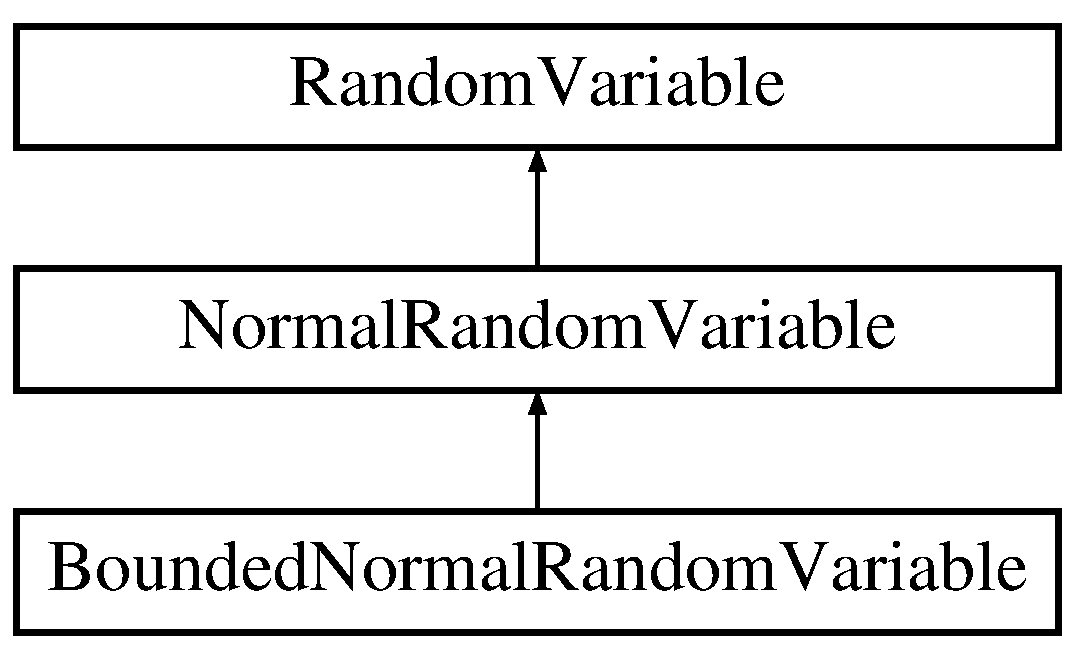
\includegraphics[height=3.000000cm]{classPecos_1_1NormalRandomVariable}
\end{center}
\end{figure}
\subsection*{Public Member Functions}
\begin{DoxyCompactItemize}
\item 
\hyperlink{classPecos_1_1NormalRandomVariable_a38f48d02679ba9bf6b7926e4618aba1e}{Normal\+Random\+Variable} ()\label{classPecos_1_1NormalRandomVariable_a38f48d02679ba9bf6b7926e4618aba1e}

\begin{DoxyCompactList}\small\item\em constructor \end{DoxyCompactList}\item 
\hyperlink{classPecos_1_1NormalRandomVariable_ad74b95737afea6cd530778462abc6fd5}{Normal\+Random\+Variable} (Real \hyperlink{classPecos_1_1NormalRandomVariable_a962ffe5a3593be370d5c883365c060f4}{mean}, Real stdev)\label{classPecos_1_1NormalRandomVariable_ad74b95737afea6cd530778462abc6fd5}

\begin{DoxyCompactList}\small\item\em alternate constructor \end{DoxyCompactList}\item 
\hyperlink{classPecos_1_1NormalRandomVariable_a297038edcbddebccbc6ef8b4bed843a4}{$\sim$\+Normal\+Random\+Variable} ()\label{classPecos_1_1NormalRandomVariable_a297038edcbddebccbc6ef8b4bed843a4}

\begin{DoxyCompactList}\small\item\em destructor \end{DoxyCompactList}\item 
Real \hyperlink{classPecos_1_1NormalRandomVariable_addd564e7f4f314e12d38df74d845f0d8}{cdf} (Real x) const \label{classPecos_1_1NormalRandomVariable_addd564e7f4f314e12d38df74d845f0d8}

\begin{DoxyCompactList}\small\item\em return the cumulative distribution function value of the random variable at x \end{DoxyCompactList}\item 
Real \hyperlink{classPecos_1_1NormalRandomVariable_a23c3b599e7e4788a9a5e9e93c3dbaf4d}{ccdf} (Real x) const \label{classPecos_1_1NormalRandomVariable_a23c3b599e7e4788a9a5e9e93c3dbaf4d}

\begin{DoxyCompactList}\small\item\em return the complementary cumulative distribution function value of the random variable at x \end{DoxyCompactList}\item 
Real \hyperlink{classPecos_1_1NormalRandomVariable_a918a1aac05ca349ea5313eebcba46c3e}{inverse\+\_\+cdf} (Real p\+\_\+cdf) const \label{classPecos_1_1NormalRandomVariable_a918a1aac05ca349ea5313eebcba46c3e}

\begin{DoxyCompactList}\small\item\em return the x value corresponding to a cumulative probability \end{DoxyCompactList}\item 
Real \hyperlink{classPecos_1_1NormalRandomVariable_afda003a1f59ff6930902cd5c8601f49b}{inverse\+\_\+ccdf} (Real p\+\_\+ccdf) const \label{classPecos_1_1NormalRandomVariable_afda003a1f59ff6930902cd5c8601f49b}

\begin{DoxyCompactList}\small\item\em return the x value corresponding to a complementary cumulative probability \end{DoxyCompactList}\item 
Real \hyperlink{classPecos_1_1NormalRandomVariable_a8ec69265f428e17c1707133cb137a819}{pdf} (Real x) const \label{classPecos_1_1NormalRandomVariable_a8ec69265f428e17c1707133cb137a819}

\begin{DoxyCompactList}\small\item\em return the value of the random variable\textquotesingle{}s probability density function at x \end{DoxyCompactList}\item 
Real \hyperlink{classPecos_1_1NormalRandomVariable_aaa7ca3718abc034be7629af5594efca0}{pdf\+\_\+gradient} (Real x) const \label{classPecos_1_1NormalRandomVariable_aaa7ca3718abc034be7629af5594efca0}

\begin{DoxyCompactList}\small\item\em return the gradient of the random variable\textquotesingle{}s probability density function at x \end{DoxyCompactList}\item 
Real \hyperlink{classPecos_1_1NormalRandomVariable_a514a0abe97269ac6e003f43683d9137e}{pdf\+\_\+hessian} (Real x) const \label{classPecos_1_1NormalRandomVariable_a514a0abe97269ac6e003f43683d9137e}

\begin{DoxyCompactList}\small\item\em return the hessian of the random variable\textquotesingle{}s probability density function at x \end{DoxyCompactList}\item 
Real \hyperlink{classPecos_1_1NormalRandomVariable_a6e2b6b6f13eedb2eb1ef3bc455a06392}{log\+\_\+pdf} (Real x) const \label{classPecos_1_1NormalRandomVariable_a6e2b6b6f13eedb2eb1ef3bc455a06392}

\begin{DoxyCompactList}\small\item\em return the value of the natural log of the random variable\textquotesingle{}s probability density function at x (useful for calculations of log density in Bayesian methods) \end{DoxyCompactList}\item 
Real \hyperlink{classPecos_1_1NormalRandomVariable_a5ccc16c04690f0c501f44c1ffae2bbd1}{log\+\_\+pdf\+\_\+gradient} (Real x) const \label{classPecos_1_1NormalRandomVariable_a5ccc16c04690f0c501f44c1ffae2bbd1}

\begin{DoxyCompactList}\small\item\em return the gradient of the natural log of the random variable\textquotesingle{}s probability density function at x (useful for defining M\+C\+MC proposal distributions in Bayesian methods) \end{DoxyCompactList}\item 
Real \hyperlink{classPecos_1_1NormalRandomVariable_a7b43f26f0f2bcdfef15d87e1f9399b33}{log\+\_\+pdf\+\_\+hessian} (Real x) const \label{classPecos_1_1NormalRandomVariable_a7b43f26f0f2bcdfef15d87e1f9399b33}

\begin{DoxyCompactList}\small\item\em return the Hessian of the natural log of the random variable\textquotesingle{}s probability density function at x (useful for defining M\+C\+MC proposal distributions in Bayesian methods) \end{DoxyCompactList}\item 
Real \hyperlink{classPecos_1_1NormalRandomVariable_acffcd338a207168a147fffe0778ccf3c}{inverse\+\_\+standard\+\_\+cdf} (Real p\+\_\+cdf) const \label{classPecos_1_1NormalRandomVariable_acffcd338a207168a147fffe0778ccf3c}

\begin{DoxyCompactList}\small\item\em return the x value for a standardized probability distribution corresponding to a cumulative probability \end{DoxyCompactList}\item 
Real \hyperlink{classPecos_1_1NormalRandomVariable_a206a02581b82f44be4a5321488a12daa}{standard\+\_\+pdf} (Real z) const \label{classPecos_1_1NormalRandomVariable_a206a02581b82f44be4a5321488a12daa}

\begin{DoxyCompactList}\small\item\em return the value of a standardized random variable\textquotesingle{}s probability density function at x \end{DoxyCompactList}\item 
Real \hyperlink{classPecos_1_1NormalRandomVariable_a1eb7deb350fc38d35e32ba7d0b96c464}{log\+\_\+standard\+\_\+pdf} (Real z) const \label{classPecos_1_1NormalRandomVariable_a1eb7deb350fc38d35e32ba7d0b96c464}

\begin{DoxyCompactList}\small\item\em return the natural log of a standardized random variable\textquotesingle{}s probability density function at x (useful for calculations of log density in Bayesian methods) \end{DoxyCompactList}\item 
Real \hyperlink{classPecos_1_1NormalRandomVariable_a73ea75d51f5415f600bebbca4a9628b7}{log\+\_\+standard\+\_\+pdf\+\_\+gradient} (Real z) const \label{classPecos_1_1NormalRandomVariable_a73ea75d51f5415f600bebbca4a9628b7}

\begin{DoxyCompactList}\small\item\em return the gradient of the natural log of a standardized random variable\textquotesingle{}s probability density function at x (useful for calculations of log density in Bayesian methods) \end{DoxyCompactList}\item 
Real \hyperlink{classPecos_1_1NormalRandomVariable_acf89562740c674e54901e97817f56b69}{log\+\_\+standard\+\_\+pdf\+\_\+hessian} (Real z) const \label{classPecos_1_1NormalRandomVariable_acf89562740c674e54901e97817f56b69}

\begin{DoxyCompactList}\small\item\em return the Hessian of the natural log of a standardized random variable\textquotesingle{}s probability density function at x (useful for calculations of log density in Bayesian methods) \end{DoxyCompactList}\item 
Real \hyperlink{classPecos_1_1NormalRandomVariable_a42e98c7343a1ce031f5481c11476fa73}{to\+\_\+standard} (Real x) const \label{classPecos_1_1NormalRandomVariable_a42e98c7343a1ce031f5481c11476fa73}

\begin{DoxyCompactList}\small\item\em scale variable value x from current to standardized distribution \end{DoxyCompactList}\item 
Real \hyperlink{classPecos_1_1NormalRandomVariable_a05e16ccd21e4fe4f3f74a1a98ae9dc74}{from\+\_\+standard} (Real z) const \label{classPecos_1_1NormalRandomVariable_a05e16ccd21e4fe4f3f74a1a98ae9dc74}

\begin{DoxyCompactList}\small\item\em scale variable value z from standardized to current distribution \end{DoxyCompactList}\item 
Real \hyperlink{classPecos_1_1NormalRandomVariable_aa891dab1ae9a225f493e3a0e5032b778}{parameter} (short dist\+\_\+param) const \label{classPecos_1_1NormalRandomVariable_aa891dab1ae9a225f493e3a0e5032b778}

\begin{DoxyCompactList}\small\item\em return the value of the named distribution parameter \end{DoxyCompactList}\item 
void \hyperlink{classPecos_1_1NormalRandomVariable_ae8e123224f588aee676d5d56d5ca900d}{parameter} (short dist\+\_\+param, Real val)\label{classPecos_1_1NormalRandomVariable_ae8e123224f588aee676d5d56d5ca900d}

\begin{DoxyCompactList}\small\item\em update the value of the named distribution parameter \end{DoxyCompactList}\item 
Real \hyperlink{classPecos_1_1NormalRandomVariable_a962ffe5a3593be370d5c883365c060f4}{mean} () const \label{classPecos_1_1NormalRandomVariable_a962ffe5a3593be370d5c883365c060f4}

\begin{DoxyCompactList}\small\item\em return the distribution mean \end{DoxyCompactList}\item 
Real \hyperlink{classPecos_1_1NormalRandomVariable_ae1fff19ce29a79d657043a598523635d}{median} () const \label{classPecos_1_1NormalRandomVariable_ae1fff19ce29a79d657043a598523635d}

\begin{DoxyCompactList}\small\item\em return the distribution mode \end{DoxyCompactList}\item 
Real \hyperlink{classPecos_1_1NormalRandomVariable_a72d3d6926edd929cb3f8e12baa655f70}{mode} () const \label{classPecos_1_1NormalRandomVariable_a72d3d6926edd929cb3f8e12baa655f70}

\begin{DoxyCompactList}\small\item\em return the distribution mode \end{DoxyCompactList}\item 
Real \hyperlink{classPecos_1_1NormalRandomVariable_a6a4ed9624d511f8a4e4f509c82cb0706}{standard\+\_\+deviation} () const \label{classPecos_1_1NormalRandomVariable_a6a4ed9624d511f8a4e4f509c82cb0706}

\begin{DoxyCompactList}\small\item\em return the distribution variance \end{DoxyCompactList}\item 
Real \hyperlink{classPecos_1_1NormalRandomVariable_a4b8b05b2a9af92dad9cc304c2925a4eb}{variance} () const \label{classPecos_1_1NormalRandomVariable_a4b8b05b2a9af92dad9cc304c2925a4eb}

\begin{DoxyCompactList}\small\item\em return the distribution variance \end{DoxyCompactList}\item 
Real\+Real\+Pair \hyperlink{classPecos_1_1NormalRandomVariable_a4bdb95a8fa5fffaa0de5102f56963cf2}{bounds} () const \label{classPecos_1_1NormalRandomVariable_a4bdb95a8fa5fffaa0de5102f56963cf2}

\begin{DoxyCompactList}\small\item\em return the distribution lower and upper bounds as a pair \end{DoxyCompactList}\item 
Real \hyperlink{classPecos_1_1NormalRandomVariable_a9ee48b3ca93459136b2e73f77873c4aa}{correlation\+\_\+warping\+\_\+factor} (const \hyperlink{classPecos_1_1RandomVariable}{Random\+Variable} \&rv, Real corr) const \label{classPecos_1_1NormalRandomVariable_a9ee48b3ca93459136b2e73f77873c4aa}

\begin{DoxyCompactList}\small\item\em compute the warping factor for correlation between the current variable and the one passed in (used in \hyperlink{classPecos_1_1NatafTransformation}{Nataf\+Transformation}) \end{DoxyCompactList}\item 
Real \hyperlink{classPecos_1_1NormalRandomVariable_af889af8adfb262c9b74f573b2a9ffc99}{dx\+\_\+ds} (short dist\+\_\+param, short u\+\_\+type, Real x, Real z) const 
\item 
Real \hyperlink{classPecos_1_1NormalRandomVariable_af6b5fc528523180bed5fc3008dcea205}{dz\+\_\+ds\+\_\+factor} (short u\+\_\+type, Real x, Real z) const 
\item 
void {\bfseries update} (Real \hyperlink{classPecos_1_1NormalRandomVariable_a962ffe5a3593be370d5c883365c060f4}{mean}, Real stdev)\label{classPecos_1_1NormalRandomVariable_a9a71c4cc1904385206f39644b461b3b3}

\end{DoxyCompactItemize}
\subsection*{Static Public Member Functions}
\begin{DoxyCompactItemize}
\item 
static Real {\bfseries pdf} (Real x, Real \hyperlink{classPecos_1_1NormalRandomVariable_a962ffe5a3593be370d5c883365c060f4}{mean}, Real std\+\_\+dev)\label{classPecos_1_1NormalRandomVariable_a1c24d3db932d840bd8876d25445fe0d2}

\item 
static Real {\bfseries cdf} (Real x, Real \hyperlink{classPecos_1_1NormalRandomVariable_a962ffe5a3593be370d5c883365c060f4}{mean}, Real std\+\_\+dev)\label{classPecos_1_1NormalRandomVariable_a997b966ecf3b793457430273db5079e3}

\item 
static Real \hyperlink{classPecos_1_1NormalRandomVariable_a1723ee7569b2b6dd6413dc9ffc0382b6}{std\+\_\+pdf} (Real z)
\item 
static Real {\bfseries mvn\+\_\+std\+\_\+pdf} (Real beta, size\+\_\+t n)\label{classPecos_1_1NormalRandomVariable_aa8b5e5701c2456b953f1c386d36e07fe}

\item 
static Real {\bfseries mvn\+\_\+std\+\_\+pdf} (const Real\+Vector \&u)\label{classPecos_1_1NormalRandomVariable_a12503add3b2cec672b8c9b50c13bf4cc}

\item 
static Real \hyperlink{classPecos_1_1NormalRandomVariable_a62b98da8336394c9e30ea9fd5e79b2e5}{std\+\_\+cdf} (Real z)
\item 
static Real {\bfseries std\+\_\+ccdf} (Real z)\label{classPecos_1_1NormalRandomVariable_aa02b173cdbee0e135e5501acc7edd639}

\item 
static Real {\bfseries inverse\+\_\+std\+\_\+cdf} (Real p\+\_\+cdf)\label{classPecos_1_1NormalRandomVariable_ad0d24d0f74c6ff422ffb64f8204e5c04}

\item 
static Real {\bfseries inverse\+\_\+std\+\_\+ccdf} (Real p\+\_\+ccdf)\label{classPecos_1_1NormalRandomVariable_ab1e233a604518e682cf7d179d3d2879a}

\item 
static Real {\bfseries log\+\_\+std\+\_\+pdf} (Real z)\label{classPecos_1_1NormalRandomVariable_a9672626f0688946d80b65a8fd041aa03}

\item 
static Real {\bfseries log\+\_\+std\+\_\+pdf\+\_\+gradient} (Real z)\label{classPecos_1_1NormalRandomVariable_a3c21a78586ff3c5eacf54ab89926f0c6}

\item 
static Real {\bfseries log\+\_\+std\+\_\+pdf\+\_\+hessian} ()\label{classPecos_1_1NormalRandomVariable_ae4d8f47aa3f234d3887059246d213335}

\item 
static Real {\bfseries log\+\_\+std\+\_\+cdf} (Real z)\label{classPecos_1_1NormalRandomVariable_ad7af5d4f067abfbda2fc15a24c992206}

\item 
static Real {\bfseries log\+\_\+std\+\_\+ccdf} (Real z)\label{classPecos_1_1NormalRandomVariable_aebae2e3981abbab367a1ecd8a4755868}

\item 
{\footnotesize template$<$typename Engine $>$ }\\static Real {\bfseries draw\+\_\+std\+\_\+sample} (Engine \&rng)\label{classPecos_1_1NormalRandomVariable_a6fcc236683df40e8eb64ea81b5e38de9}

\end{DoxyCompactItemize}
\subsection*{Protected Attributes}
\begin{DoxyCompactItemize}
\item 
Real \hyperlink{classPecos_1_1NormalRandomVariable_ac9a37579d73aacb9cbab27e3be731e64}{gauss\+Mean}\label{classPecos_1_1NormalRandomVariable_ac9a37579d73aacb9cbab27e3be731e64}

\begin{DoxyCompactList}\small\item\em mean of Gaussian random variable \end{DoxyCompactList}\item 
Real \hyperlink{classPecos_1_1NormalRandomVariable_aab6c8417eeb34557962638736c554927}{gauss\+Std\+Dev}\label{classPecos_1_1NormalRandomVariable_aab6c8417eeb34557962638736c554927}

\begin{DoxyCompactList}\small\item\em standard deviation of Gaussian random variable \end{DoxyCompactList}\end{DoxyCompactItemize}
\subsection*{Additional Inherited Members}


\subsection{Detailed Description}
Derived random variable class for Gaussian random variables. 

Manages mean and standard deviation. 

\subsection{Member Function Documentation}
\index{Pecos\+::\+Normal\+Random\+Variable@{Pecos\+::\+Normal\+Random\+Variable}!dx\+\_\+ds@{dx\+\_\+ds}}
\index{dx\+\_\+ds@{dx\+\_\+ds}!Pecos\+::\+Normal\+Random\+Variable@{Pecos\+::\+Normal\+Random\+Variable}}
\subsubsection[{\texorpdfstring{dx\+\_\+ds(short dist\+\_\+param, short u\+\_\+type, Real x, Real z) const }{dx_ds(short dist_param, short u_type, Real x, Real z) const }}]{\setlength{\rightskip}{0pt plus 5cm}Real dx\+\_\+ds (
\begin{DoxyParamCaption}
\item[{short}]{dist\+\_\+param, }
\item[{short}]{u\+\_\+type, }
\item[{Real}]{x, }
\item[{Real}]{z}
\end{DoxyParamCaption}
) const\hspace{0.3cm}{\ttfamily [inline]}, {\ttfamily [virtual]}}\label{classPecos_1_1NormalRandomVariable_af889af8adfb262c9b74f573b2a9ffc99}
dx/ds is derived by differentiating \hyperlink{classPecos_1_1NatafTransformation_a5feeecf846fc017c5a28eccb4e955dc1}{Nataf\+Transformation\+::trans\+\_\+\+Z\+\_\+to\+\_\+\+X()} with respect to distribution parameter s. dz/ds is zero if uncorrelated, while \hyperlink{classPecos_1_1NormalRandomVariable_af6b5fc528523180bed5fc3008dcea205}{dz\+\_\+ds\+\_\+factor()} manages contributions in the correlated case. 

Reimplemented from \hyperlink{classPecos_1_1RandomVariable_af889af8adfb262c9b74f573b2a9ffc99}{Random\+Variable}.



References Normal\+Random\+Variable\+::dz\+\_\+ds\+\_\+factor().



Referenced by Normal\+Random\+Variable\+::parameter().

\index{Pecos\+::\+Normal\+Random\+Variable@{Pecos\+::\+Normal\+Random\+Variable}!dz\+\_\+ds\+\_\+factor@{dz\+\_\+ds\+\_\+factor}}
\index{dz\+\_\+ds\+\_\+factor@{dz\+\_\+ds\+\_\+factor}!Pecos\+::\+Normal\+Random\+Variable@{Pecos\+::\+Normal\+Random\+Variable}}
\subsubsection[{\texorpdfstring{dz\+\_\+ds\+\_\+factor(short u\+\_\+type, Real x, Real z) const }{dz_ds_factor(short u_type, Real x, Real z) const }}]{\setlength{\rightskip}{0pt plus 5cm}Real dz\+\_\+ds\+\_\+factor (
\begin{DoxyParamCaption}
\item[{short}]{u\+\_\+type, }
\item[{Real}]{x, }
\item[{Real}]{z}
\end{DoxyParamCaption}
) const\hspace{0.3cm}{\ttfamily [inline]}, {\ttfamily [virtual]}}\label{classPecos_1_1NormalRandomVariable_af6b5fc528523180bed5fc3008dcea205}
dx/ds is derived by differentiating \hyperlink{classPecos_1_1NatafTransformation_a5feeecf846fc017c5a28eccb4e955dc1}{Nataf\+Transformation\+::trans\+\_\+\+Z\+\_\+to\+\_\+\+X()} with respect to distribution parameter s. For the uncorrelated case, u and z are constants. For the correlated case, u is a constant, but z(s) = L(s) u due to Nataf dependence on s and dz/ds = d\+L/ds u. 

Reimplemented from \hyperlink{classPecos_1_1RandomVariable_af6b5fc528523180bed5fc3008dcea205}{Random\+Variable}.



References Normal\+Random\+Variable\+::cdf(), Normal\+Random\+Variable\+::gauss\+Mean, Normal\+Random\+Variable\+::gauss\+Std\+Dev, Normal\+Random\+Variable\+::mean(), and Normal\+Random\+Variable\+::pdf().



Referenced by Normal\+Random\+Variable\+::dx\+\_\+ds().

\index{Pecos\+::\+Normal\+Random\+Variable@{Pecos\+::\+Normal\+Random\+Variable}!std\+\_\+pdf@{std\+\_\+pdf}}
\index{std\+\_\+pdf@{std\+\_\+pdf}!Pecos\+::\+Normal\+Random\+Variable@{Pecos\+::\+Normal\+Random\+Variable}}
\subsubsection[{\texorpdfstring{std\+\_\+pdf(\+Real z)}{std_pdf(Real z)}}]{\setlength{\rightskip}{0pt plus 5cm}Real std\+\_\+pdf (
\begin{DoxyParamCaption}
\item[{Real}]{z}
\end{DoxyParamCaption}
)\hspace{0.3cm}{\ttfamily [inline]}, {\ttfamily [static]}}\label{classPecos_1_1NormalRandomVariable_a1723ee7569b2b6dd6413dc9ffc0382b6}
returns a cumulative probability $<$ 0.\+5 for negative z and a cumulative probability $>$ 0.\+5 for positive z. 

Referenced by Bounded\+Lognormal\+Random\+Variable\+::dx\+\_\+ds(), Bounded\+Normal\+Random\+Variable\+::dx\+\_\+ds(), Loguniform\+Random\+Variable\+::dz\+\_\+ds\+\_\+factor(), Triangular\+Random\+Variable\+::dz\+\_\+ds\+\_\+factor(), Frechet\+Random\+Variable\+::dz\+\_\+ds\+\_\+factor(), Weibull\+Random\+Variable\+::dz\+\_\+ds\+\_\+factor(), Bounded\+Normal\+Random\+Variable\+::dz\+\_\+ds\+\_\+factor(), Bounded\+Lognormal\+Random\+Variable\+::dz\+\_\+ds\+\_\+factor(), Gumbel\+Random\+Variable\+::dz\+\_\+ds\+\_\+factor(), Uniform\+Random\+Variable\+::dz\+\_\+ds\+\_\+factor(), Exponential\+Random\+Variable\+::dz\+\_\+ds\+\_\+factor(), Numeric\+Gen\+Orthog\+Polynomial\+::hermite\+\_\+unbounded\+\_\+integral(), Nataf\+Transformation\+::hessian\+\_\+d2\+X\+\_\+d\+Z2(), Nataf\+Transformation\+::jacobian\+\_\+d\+X\+\_\+d\+Z(), Nataf\+Transformation\+::jacobian\+\_\+d\+Z\+\_\+d\+X(), Bounded\+Normal\+Random\+Variable\+::mean(), Bounded\+Normal\+Random\+Variable\+::moments(), Normal\+Random\+Variable\+::standard\+\_\+pdf(), Probability\+Transformation\+::u\+\_\+pdf(), Bounded\+Normal\+Random\+Variable\+::variance(), Bounded\+Lognormal\+Random\+Variable\+::$\sim$\+Bounded\+Lognormal\+Random\+Variable(), and Bounded\+Normal\+Random\+Variable\+::$\sim$\+Bounded\+Normal\+Random\+Variable().

\index{Pecos\+::\+Normal\+Random\+Variable@{Pecos\+::\+Normal\+Random\+Variable}!std\+\_\+cdf@{std\+\_\+cdf}}
\index{std\+\_\+cdf@{std\+\_\+cdf}!Pecos\+::\+Normal\+Random\+Variable@{Pecos\+::\+Normal\+Random\+Variable}}
\subsubsection[{\texorpdfstring{std\+\_\+cdf(\+Real z)}{std_cdf(Real z)}}]{\setlength{\rightskip}{0pt plus 5cm}Real std\+\_\+cdf (
\begin{DoxyParamCaption}
\item[{Real}]{z}
\end{DoxyParamCaption}
)\hspace{0.3cm}{\ttfamily [inline]}, {\ttfamily [static]}}\label{classPecos_1_1NormalRandomVariable_a62b98da8336394c9e30ea9fd5e79b2e5}
returns a cumulative probability $<$ 0.\+5 for negative z and a cumulative probability $>$ 0.\+5 for positive z. 

Referenced by Bounded\+Lognormal\+Random\+Variable\+::ccdf(), Bounded\+Normal\+Random\+Variable\+::ccdf(), Loguniform\+Random\+Variable\+::dx\+\_\+ds(), Triangular\+Random\+Variable\+::dx\+\_\+ds(), Bounded\+Normal\+Random\+Variable\+::dx\+\_\+ds(), Bounded\+Lognormal\+Random\+Variable\+::dx\+\_\+ds(), Frechet\+Random\+Variable\+::dz\+\_\+ds\+\_\+factor(), Bounded\+Lognormal\+Random\+Variable\+::dz\+\_\+ds\+\_\+factor(), Bounded\+Normal\+Random\+Variable\+::dz\+\_\+ds\+\_\+factor(), Gumbel\+Random\+Variable\+::dz\+\_\+ds\+\_\+factor(), Bounded\+Lognormal\+Random\+Variable\+::inverse\+\_\+ccdf(), Bounded\+Normal\+Random\+Variable\+::inverse\+\_\+ccdf(), Bounded\+Lognormal\+Random\+Variable\+::inverse\+\_\+cdf(), Bounded\+Normal\+Random\+Variable\+::inverse\+\_\+cdf(), Bounded\+Lognormal\+Random\+Variable\+::log\+\_\+pdf(), Bounded\+Normal\+Random\+Variable\+::log\+\_\+pdf(), Bounded\+Normal\+Random\+Variable\+::mean(), Bounded\+Lognormal\+Random\+Variable\+::mean(), Bounded\+Normal\+Random\+Variable\+::moments(), Bounded\+Lognormal\+Random\+Variable\+::moments(), Nataf\+Transformation\+::trans\+\_\+\+Z\+\_\+to\+\_\+\+X(), Bounded\+Normal\+Random\+Variable\+::variance(), Bounded\+Lognormal\+Random\+Variable\+::$\sim$\+Bounded\+Lognormal\+Random\+Variable(), and Bounded\+Normal\+Random\+Variable\+::$\sim$\+Bounded\+Normal\+Random\+Variable().



The documentation for this class was generated from the following file\+:\begin{DoxyCompactItemize}
\item 
Normal\+Random\+Variable.\+hpp\end{DoxyCompactItemize}

\section{Numeric\+Gen\+Orthog\+Polynomial Class Reference}
\label{classPecos_1_1NumericGenOrthogPolynomial}\index{Numeric\+Gen\+Orthog\+Polynomial@{Numeric\+Gen\+Orthog\+Polynomial}}


Derived orthogonal polynomial class for numerically-\/generated orthogonal polynomials.  


Inheritance diagram for Numeric\+Gen\+Orthog\+Polynomial\+:\begin{figure}[H]
\begin{center}
\leavevmode
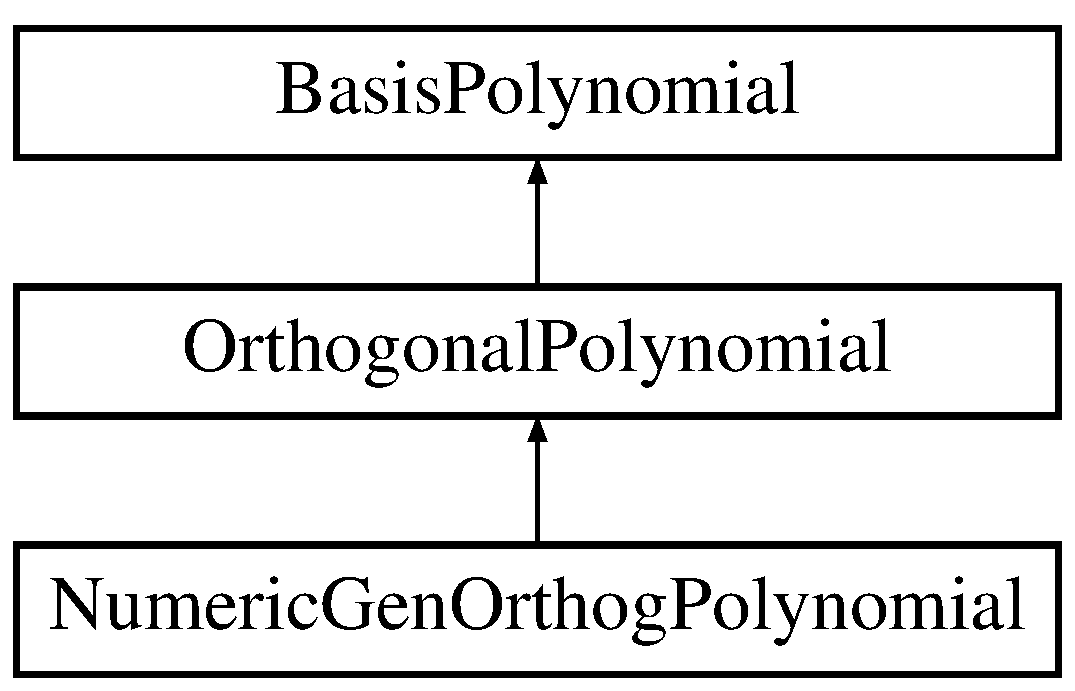
\includegraphics[height=3.000000cm]{classPecos_1_1NumericGenOrthogPolynomial}
\end{center}
\end{figure}
\subsection*{Public Member Functions}
\begin{DoxyCompactItemize}
\item 
\hyperlink{classPecos_1_1NumericGenOrthogPolynomial_aed4a0fd6a1af04dc56a264c5678a2fac}{Numeric\+Gen\+Orthog\+Polynomial} ()\label{classPecos_1_1NumericGenOrthogPolynomial_aed4a0fd6a1af04dc56a264c5678a2fac}

\begin{DoxyCompactList}\small\item\em default constructor \end{DoxyCompactList}\item 
\hyperlink{classPecos_1_1NumericGenOrthogPolynomial_aa0cdaf73221c07cee322ba48adc4dea5}{$\sim$\+Numeric\+Gen\+Orthog\+Polynomial} ()\label{classPecos_1_1NumericGenOrthogPolynomial_aa0cdaf73221c07cee322ba48adc4dea5}

\begin{DoxyCompactList}\small\item\em destructor \end{DoxyCompactList}\item 
Real \hyperlink{classPecos_1_1NumericGenOrthogPolynomial_a7ad109946452e70e95aa68ffefd2c37f}{alpha\+\_\+recursion} (unsigned short order)\label{classPecos_1_1NumericGenOrthogPolynomial_a7ad109946452e70e95aa68ffefd2c37f}

\begin{DoxyCompactList}\small\item\em calculate and return alpha3\+TR\mbox{[}order\mbox{]} \end{DoxyCompactList}\item 
Real \hyperlink{classPecos_1_1NumericGenOrthogPolynomial_aa4e36e6a9911ff7214ebc87e505702f5}{beta\+\_\+recursion} (unsigned short order)\label{classPecos_1_1NumericGenOrthogPolynomial_aa4e36e6a9911ff7214ebc87e505702f5}

\begin{DoxyCompactList}\small\item\em calculate and return beta3\+TR\mbox{[}order\mbox{]} \end{DoxyCompactList}\item 
void \hyperlink{classPecos_1_1NumericGenOrthogPolynomial_ae391dd223bd9a29d15f7d75e7305b7b7}{bounded\+\_\+normal\+\_\+distribution} (Real mean, Real std\+\_\+dev, Real l\+\_\+bnd, Real u\+\_\+bnd)\label{classPecos_1_1NumericGenOrthogPolynomial_ae391dd223bd9a29d15f7d75e7305b7b7}

\begin{DoxyCompactList}\small\item\em set distribution type and parameters for a B\+O\+U\+N\+D\+E\+D\+\_\+\+N\+O\+R\+M\+AL distribution \end{DoxyCompactList}\item 
void \hyperlink{classPecos_1_1NumericGenOrthogPolynomial_ab467d60674465716b7a4b958e4c48875}{lognormal\+\_\+distribution} (Real lambda, Real zeta)\label{classPecos_1_1NumericGenOrthogPolynomial_ab467d60674465716b7a4b958e4c48875}

\begin{DoxyCompactList}\small\item\em set distribution type and parameters for a L\+O\+G\+N\+O\+R\+M\+AL distribution \end{DoxyCompactList}\item 
void \hyperlink{classPecos_1_1NumericGenOrthogPolynomial_aaa0279e513aed19ffce83c78553c1b8c}{bounded\+\_\+lognormal\+\_\+distribution} (Real lambda, Real zeta, Real l\+\_\+bnd, Real u\+\_\+bnd)\label{classPecos_1_1NumericGenOrthogPolynomial_aaa0279e513aed19ffce83c78553c1b8c}

\begin{DoxyCompactList}\small\item\em set distribution type and parameters for a B\+O\+U\+N\+D\+E\+D\+\_\+\+L\+O\+G\+N\+O\+R\+M\+AL distribution \end{DoxyCompactList}\item 
void \hyperlink{classPecos_1_1NumericGenOrthogPolynomial_afcfe468921c964e1935b9ed42990e51f}{loguniform\+\_\+distribution} (Real l\+\_\+bnd, Real u\+\_\+bnd)\label{classPecos_1_1NumericGenOrthogPolynomial_afcfe468921c964e1935b9ed42990e51f}

\begin{DoxyCompactList}\small\item\em set distribution type and parameters for a L\+O\+G\+U\+N\+I\+F\+O\+RM distribution \end{DoxyCompactList}\item 
void \hyperlink{classPecos_1_1NumericGenOrthogPolynomial_aa3e5afc92b1c583b0d0c3097074b862c}{triangular\+\_\+distribution} (Real l\+\_\+bnd, Real mode, Real u\+\_\+bnd)\label{classPecos_1_1NumericGenOrthogPolynomial_aa3e5afc92b1c583b0d0c3097074b862c}

\begin{DoxyCompactList}\small\item\em set distribution type and parameters for a T\+R\+I\+A\+N\+G\+U\+L\+AR distribution \end{DoxyCompactList}\item 
void \hyperlink{classPecos_1_1NumericGenOrthogPolynomial_a5a1cab747675e9bf5fef2d5a34acd23b}{gumbel\+\_\+distribution} (Real alpha, Real beta)\label{classPecos_1_1NumericGenOrthogPolynomial_a5a1cab747675e9bf5fef2d5a34acd23b}

\begin{DoxyCompactList}\small\item\em set distribution type and parameters for a G\+U\+M\+B\+EL distribution \end{DoxyCompactList}\item 
void \hyperlink{classPecos_1_1NumericGenOrthogPolynomial_ade2a656052c3e7822d99e007b0793f98}{frechet\+\_\+distribution} (Real alpha, Real beta)\label{classPecos_1_1NumericGenOrthogPolynomial_ade2a656052c3e7822d99e007b0793f98}

\begin{DoxyCompactList}\small\item\em set distribution type and parameters for a F\+R\+E\+C\+H\+ET distribution \end{DoxyCompactList}\item 
void \hyperlink{classPecos_1_1NumericGenOrthogPolynomial_ade0a6ad5814d47eea75c8ebea6db7227}{weibull\+\_\+distribution} (Real alpha, Real beta)\label{classPecos_1_1NumericGenOrthogPolynomial_ade0a6ad5814d47eea75c8ebea6db7227}

\begin{DoxyCompactList}\small\item\em set distribution type and parameters for a W\+E\+I\+B\+U\+LL distribution \end{DoxyCompactList}\item 
void \hyperlink{classPecos_1_1NumericGenOrthogPolynomial_a5b7f2dbecfc759d1370516a0387c296b}{histogram\+\_\+bin\+\_\+distribution} (const Real\+Real\+Map \&bin\+\_\+pairs)\label{classPecos_1_1NumericGenOrthogPolynomial_a5b7f2dbecfc759d1370516a0387c296b}

\begin{DoxyCompactList}\small\item\em set distribution type and parameters for a H\+I\+S\+T\+O\+G\+R\+A\+M\+\_\+\+B\+IN distribution \end{DoxyCompactList}\item 
void \hyperlink{classPecos_1_1NumericGenOrthogPolynomial_a1ed6582d7b2ecd6216c1675eeeee1e63}{histogram\+\_\+pt\+\_\+distribution} (const Int\+Real\+Map \&bin\+\_\+pairs)\label{classPecos_1_1NumericGenOrthogPolynomial_a1ed6582d7b2ecd6216c1675eeeee1e63}

\begin{DoxyCompactList}\small\item\em set distribution type and parameters for a H\+I\+S\+T\+O\+G\+R\+A\+M\+\_\+\+P\+T\+\_\+\+I\+NT distribution \end{DoxyCompactList}\item 
void \hyperlink{classPecos_1_1NumericGenOrthogPolynomial_a9c2ae33555e991263e00cca0e03b8173}{histogram\+\_\+pt\+\_\+distribution} (const String\+Real\+Map \&bin\+\_\+pairs)\label{classPecos_1_1NumericGenOrthogPolynomial_a9c2ae33555e991263e00cca0e03b8173}

\begin{DoxyCompactList}\small\item\em set distribution type and parameters for a H\+I\+S\+T\+O\+G\+R\+A\+M\+\_\+\+P\+T\+\_\+\+S\+T\+R\+I\+NG distribution \end{DoxyCompactList}\item 
void \hyperlink{classPecos_1_1NumericGenOrthogPolynomial_a7594170792e5fc5c27b94e61fa753d88}{histogram\+\_\+pt\+\_\+distribution} (const Real\+Real\+Map \&bin\+\_\+pairs)\label{classPecos_1_1NumericGenOrthogPolynomial_a7594170792e5fc5c27b94e61fa753d88}

\begin{DoxyCompactList}\small\item\em set distribution type and parameters for a H\+I\+S\+T\+O\+G\+R\+A\+M\+\_\+\+P\+T\+\_\+\+R\+E\+AL distribution \end{DoxyCompactList}\item 
void \hyperlink{classPecos_1_1NumericGenOrthogPolynomial_a738108531d8a83dd1a9c6021c76e6bee}{coefficients\+\_\+norms\+\_\+flag} (bool flag)\label{classPecos_1_1NumericGenOrthogPolynomial_a738108531d8a83dd1a9c6021c76e6bee}

\begin{DoxyCompactList}\small\item\em set coeffs\+Norms\+Flag \end{DoxyCompactList}\end{DoxyCompactItemize}
\subsection*{Protected Member Functions}
\begin{DoxyCompactItemize}
\item 
Real \hyperlink{classPecos_1_1NumericGenOrthogPolynomial_a8792a858ac05a2158880e876f9da2019}{type1\+\_\+value} (Real x, unsigned short order)
\begin{DoxyCompactList}\small\item\em retrieve the value of the n\+\_\+th type 1 polynomial for a given parameter x using traditional characteristic polynomial formulation \end{DoxyCompactList}\item 
Real \hyperlink{classPecos_1_1NumericGenOrthogPolynomial_aac6751aa35bf5fcb42c520a322fc26dc}{type1\+\_\+gradient} (Real x, unsigned short order)
\begin{DoxyCompactList}\small\item\em retrieve the gradient of the n\+\_\+th type 1 polynomial for a given parameter x using traditional characteristic polynomial formulation \end{DoxyCompactList}\item 
Real \hyperlink{classPecos_1_1NumericGenOrthogPolynomial_ae957c8c2e7ea13728bafbad0c9b2996e}{type1\+\_\+hessian} (Real x, unsigned short order)
\begin{DoxyCompactList}\small\item\em retrieve the Hessian of the n\+\_\+th type 1 polynomial for a given parameter x using traditional characteristic polynomial formulation \end{DoxyCompactList}\item 
Real \hyperlink{classPecos_1_1NumericGenOrthogPolynomial_a77c0dbb874af1190d448d01da6efbe4e}{norm\+\_\+squared} (unsigned short order)
\begin{DoxyCompactList}\small\item\em returns the norm-\/squared of the n\+\_\+th order polynomial defined by the inner product $<$Poly\+\_\+n, Poly\+\_\+n$>$ = $\vert$$\vert$\+Poly\+\_\+n$\vert$$\vert$$^\wedge$2 \end{DoxyCompactList}\item 
const Real\+Array \& \hyperlink{classPecos_1_1NumericGenOrthogPolynomial_a10873b28f1284aff4ea214e00c4f86dd}{collocation\+\_\+points} (unsigned short order)
\begin{DoxyCompactList}\small\item\em return collocation points corresponding to orthogonal polynomial order n \end{DoxyCompactList}\item 
const Real\+Array \& \hyperlink{classPecos_1_1NumericGenOrthogPolynomial_aa010321cf47465dca5725fa15ba58bf6}{type1\+\_\+collocation\+\_\+weights} (unsigned short order)
\begin{DoxyCompactList}\small\item\em return the type 1 collocation weights corresponding to a point set of size order \end{DoxyCompactList}\item 
bool \hyperlink{classPecos_1_1NumericGenOrthogPolynomial_abc2afafc150f648667a41e0ce656b6da}{parameterized} () const \label{classPecos_1_1NumericGenOrthogPolynomial_abc2afafc150f648667a41e0ce656b6da}

\begin{DoxyCompactList}\small\item\em return whether a derived \hyperlink{classPecos_1_1BasisPolynomial}{Basis\+Polynomial} type supports parameterization \end{DoxyCompactList}\item 
Real \hyperlink{classPecos_1_1NumericGenOrthogPolynomial_a8c1e8d014e82efc5a1c20f973b5bc715}{length\+\_\+scale} () const 
\item 
void \hyperlink{classPecos_1_1NumericGenOrthogPolynomial_ad1f50a6d03d3b48687bf9c4ca889b389}{precompute\+\_\+rules} (unsigned short order)\label{classPecos_1_1NumericGenOrthogPolynomial_ad1f50a6d03d3b48687bf9c4ca889b389}

\begin{DoxyCompactList}\small\item\em precompute quadrature rules up to specified order \end{DoxyCompactList}\end{DoxyCompactItemize}
\subsection*{Private Member Functions}
\begin{DoxyCompactItemize}
\item 
void \hyperlink{classPecos_1_1NumericGenOrthogPolynomial_a4695676473df7032b5cf8d8939fa63f2}{solve\+\_\+eigenproblem} (unsigned short m)
\begin{DoxyCompactList}\small\item\em solve a symmetric tridiagonal eigenvalue problem for the Gauss points and weights for an orthogonal polynomial of order m \end{DoxyCompactList}\item 
void \hyperlink{classPecos_1_1NumericGenOrthogPolynomial_a37403d7492f13f1482ba45befc66c886}{polynomial\+\_\+recursion} (Real\+Vector \&poly\+\_\+coeffs\+\_\+ip1, Real alpha\+\_\+i, const Real\+Vector \&poly\+\_\+coeffs\+\_\+i, Real beta\+\_\+i, const Real\+Vector \&poly\+\_\+coeffs\+\_\+im1)\label{classPecos_1_1NumericGenOrthogPolynomial_a37403d7492f13f1482ba45befc66c886}

\begin{DoxyCompactList}\small\item\em compute three point recursion for poly\+Coeffs\mbox{[}i+1\mbox{]} \end{DoxyCompactList}\item 
void \hyperlink{classPecos_1_1NumericGenOrthogPolynomial_aa23ca624e849bda93121c362fa281a11}{polynomial\+\_\+recursion} (Real\+Vector \&poly\+\_\+coeffs\+\_\+ip1, Real alpha\+\_\+i, const Real\+Vector \&poly\+\_\+coeffs\+\_\+i)\label{classPecos_1_1NumericGenOrthogPolynomial_aa23ca624e849bda93121c362fa281a11}

\begin{DoxyCompactList}\small\item\em compute truncated three point recursion for poly\+Coeffs\mbox{[}i+1\mbox{]} \end{DoxyCompactList}\item 
Real \hyperlink{classPecos_1_1NumericGenOrthogPolynomial_aa650c71abdded126ba7dccda064d1883}{inner\+\_\+product} (const Real\+Vector \&poly\+\_\+coeffs1, const Real\+Vector \&poly\+\_\+coeffs2)\label{classPecos_1_1NumericGenOrthogPolynomial_aa650c71abdded126ba7dccda064d1883}

\begin{DoxyCompactList}\small\item\em compute inner product of specified polynomial orders \end{DoxyCompactList}\item 
Real \hyperlink{classPecos_1_1NumericGenOrthogPolynomial_accf380ff2a3ff767346a92dc62048c1c}{hermite\+\_\+unbounded\+\_\+integral} (const Real\+Vector \&poly\+\_\+coeffs1, const Real\+Vector \&poly\+\_\+coeffs2, N\+G\+F\+P\+Type weight\+\_\+fn)\label{classPecos_1_1NumericGenOrthogPolynomial_accf380ff2a3ff767346a92dc62048c1c}

\begin{DoxyCompactList}\small\item\em compute an unbounded integral using Gauss-\/\+Hermite integration \end{DoxyCompactList}\item 
Real \hyperlink{classPecos_1_1NumericGenOrthogPolynomial_a721564810dcb06e9312fb31460c2ee21}{fejer\+\_\+unbounded\+\_\+integral} (const Real\+Vector \&poly\+\_\+coeffs1, const Real\+Vector \&poly\+\_\+coeffs2, N\+G\+F\+P\+Type weight\+\_\+fn, unsigned short quad\+\_\+order)\label{classPecos_1_1NumericGenOrthogPolynomial_a721564810dcb06e9312fb31460c2ee21}

\begin{DoxyCompactList}\small\item\em compute an unbounded integral using Fejer integration and a change of variables \end{DoxyCompactList}\item 
Real \hyperlink{classPecos_1_1NumericGenOrthogPolynomial_ae17c3dfbaf740f88bc54e871d100e31b}{laguerre\+\_\+semibounded\+\_\+integral} (const Real\+Vector \&poly\+\_\+coeffs1, const Real\+Vector \&poly\+\_\+coeffs2, N\+G\+F\+P\+Type weight\+\_\+fn)\label{classPecos_1_1NumericGenOrthogPolynomial_ae17c3dfbaf740f88bc54e871d100e31b}

\begin{DoxyCompactList}\small\item\em compute a semibounded integral using Gauss-\/\+Laguerre integration \end{DoxyCompactList}\item 
Real \hyperlink{classPecos_1_1NumericGenOrthogPolynomial_a727a5700d623d38660a42878f1c2aa5e}{fejer\+\_\+semibounded\+\_\+integral} (const Real\+Vector \&poly\+\_\+coeffs1, const Real\+Vector \&poly\+\_\+coeffs2, N\+G\+F\+P\+Type weight\+\_\+fn, unsigned short quad\+\_\+order)\label{classPecos_1_1NumericGenOrthogPolynomial_a727a5700d623d38660a42878f1c2aa5e}

\begin{DoxyCompactList}\small\item\em compute a semibounded integral using Fejer integration and a change of variables \end{DoxyCompactList}\item 
Real \hyperlink{classPecos_1_1NumericGenOrthogPolynomial_af77a17f10ee8f8567e5be5bc77ec4e55}{legendre\+\_\+bounded\+\_\+integral} (const Real\+Vector \&poly\+\_\+coeffs1, const Real\+Vector \&poly\+\_\+coeffs2, N\+G\+F\+P\+Type weight\+\_\+fn, Real start, Real end)\label{classPecos_1_1NumericGenOrthogPolynomial_af77a17f10ee8f8567e5be5bc77ec4e55}

\begin{DoxyCompactList}\small\item\em compute a bounded integral over the specified range using Gauss-\/\+Legendre integration \end{DoxyCompactList}\item 
Real \hyperlink{classPecos_1_1NumericGenOrthogPolynomial_ab9e633f52b778c0e737b90852cb0ab31}{cc\+\_\+bounded\+\_\+integral} (const Real\+Vector \&poly\+\_\+coeffs1, const Real\+Vector \&poly\+\_\+coeffs2, N\+G\+F\+P\+Type weight\+\_\+fn, Real start, Real end, unsigned short quad\+\_\+order)\label{classPecos_1_1NumericGenOrthogPolynomial_ab9e633f52b778c0e737b90852cb0ab31}

\begin{DoxyCompactList}\small\item\em compute a bounded integral over the specified range using Clenshaw-\/\+Curtis integration \end{DoxyCompactList}\item 
Real \hyperlink{classPecos_1_1NumericGenOrthogPolynomial_a0c1eb0747d53f80138f824d23a61d42a}{riemann\+\_\+bounded\+\_\+integral} (const Real\+Vector \&poly\+\_\+coeffs1, const Real\+Vector \&poly\+\_\+coeffs2, N\+G\+F\+P\+Type weight\+\_\+fn, Real start, Real end)\label{classPecos_1_1NumericGenOrthogPolynomial_a0c1eb0747d53f80138f824d23a61d42a}

\begin{DoxyCompactList}\small\item\em compute a bounded integral over the specified range using Riemann sums \end{DoxyCompactList}\item 
Real \hyperlink{classPecos_1_1NumericGenOrthogPolynomial_a0cf9a7908a8f181ea6109a0e9e70de2a}{native\+\_\+quadrature\+\_\+integral} (const Real\+Vector \&poly\+\_\+coeffs1, const Real\+Vector \&poly\+\_\+coeffs2)\label{classPecos_1_1NumericGenOrthogPolynomial_a0cf9a7908a8f181ea6109a0e9e70de2a}

\begin{DoxyCompactList}\small\item\em compute an integral using the native Gaussian quadrature rule (up to order 2m-\/1 based on colloc\+Points and colloc\+Weights of order m) \end{DoxyCompactList}\item 
Real \hyperlink{classPecos_1_1NumericGenOrthogPolynomial_a36a2f2a688905b357c9aec50c32934e2}{type1\+\_\+value} (Real x, const Real\+Vector \&poly\+\_\+coeffs)\label{classPecos_1_1NumericGenOrthogPolynomial_a36a2f2a688905b357c9aec50c32934e2}

\begin{DoxyCompactList}\small\item\em retrieve the value of the 1-\/D generated polynomial (of given coefficients) for a given parameter value \end{DoxyCompactList}\item 
Real \hyperlink{classPecos_1_1NumericGenOrthogPolynomial_a28912cbd5aeeb5fa8f25186709c61393}{type1\+\_\+gradient} (Real x, const Real\+Vector \&poly\+\_\+coeffs)\label{classPecos_1_1NumericGenOrthogPolynomial_a28912cbd5aeeb5fa8f25186709c61393}

\begin{DoxyCompactList}\small\item\em retrieve the gradient of the 1-\/D generated polynomial (of given coefficients) with respect to its dimension for a given parameter value \end{DoxyCompactList}\item 
Real \hyperlink{classPecos_1_1NumericGenOrthogPolynomial_a8c6da1fc223948815cf8430fa34c6f92}{type1\+\_\+hessian} (Real x, const Real\+Vector \&poly\+\_\+coeffs)\label{classPecos_1_1NumericGenOrthogPolynomial_a8c6da1fc223948815cf8430fa34c6f92}

\begin{DoxyCompactList}\small\item\em retrieve the Hessian of the 1-\/D generated polynomial (of given coefficients) with respect to its dimension for a given parameter value \end{DoxyCompactList}\end{DoxyCompactItemize}
\subsection*{Static Private Member Functions}
\begin{DoxyCompactItemize}
\item 
static Real \hyperlink{classPecos_1_1NumericGenOrthogPolynomial_a984945a7eb3ccfbb71c04afb58f004e6}{bounded\+\_\+normal\+\_\+pdf} (Real x, const Real\+Vector \&params)\label{classPecos_1_1NumericGenOrthogPolynomial_a984945a7eb3ccfbb71c04afb58f004e6}

\begin{DoxyCompactList}\small\item\em thin wrapper for bounded\+\_\+normal\+\_\+pdf for N\+G\+F\+P\+Type A\+PI \end{DoxyCompactList}\item 
static Real \hyperlink{classPecos_1_1NumericGenOrthogPolynomial_a0e518b41ad31d7637ca61353a49677e8}{lognormal\+\_\+pdf} (Real x, const Real\+Vector \&params)\label{classPecos_1_1NumericGenOrthogPolynomial_a0e518b41ad31d7637ca61353a49677e8}

\begin{DoxyCompactList}\small\item\em thin wrapper for lognormal\+\_\+pdf for N\+G\+F\+P\+Type A\+PI \end{DoxyCompactList}\item 
static Real \hyperlink{classPecos_1_1NumericGenOrthogPolynomial_a18a2e54f42d2d707515a8e3db7f300a3}{bounded\+\_\+lognormal\+\_\+pdf} (Real x, const Real\+Vector \&params)\label{classPecos_1_1NumericGenOrthogPolynomial_a18a2e54f42d2d707515a8e3db7f300a3}

\begin{DoxyCompactList}\small\item\em thin wrapper for bounded\+\_\+lognormal\+\_\+pdf for N\+G\+F\+P\+Type A\+PI \end{DoxyCompactList}\item 
static Real \hyperlink{classPecos_1_1NumericGenOrthogPolynomial_a531874fbf054cc3f2f54700e44476cf9}{loguniform\+\_\+pdf} (Real x, const Real\+Vector \&params)\label{classPecos_1_1NumericGenOrthogPolynomial_a531874fbf054cc3f2f54700e44476cf9}

\begin{DoxyCompactList}\small\item\em thin wrapper for loguniform\+\_\+pdf for N\+G\+F\+P\+Type A\+PI \end{DoxyCompactList}\item 
static Real \hyperlink{classPecos_1_1NumericGenOrthogPolynomial_a9d18b08dbb5c90ed33f9d8fb820fcf30}{triangular\+\_\+pdf} (Real x, const Real\+Vector \&params)\label{classPecos_1_1NumericGenOrthogPolynomial_a9d18b08dbb5c90ed33f9d8fb820fcf30}

\begin{DoxyCompactList}\small\item\em thin wrapper for triangular\+\_\+pdf for N\+G\+F\+P\+Type A\+PI \end{DoxyCompactList}\item 
static Real \hyperlink{classPecos_1_1NumericGenOrthogPolynomial_a5644545bfb9382ef39793c479c47752a}{gumbel\+\_\+pdf} (Real x, const Real\+Vector \&params)\label{classPecos_1_1NumericGenOrthogPolynomial_a5644545bfb9382ef39793c479c47752a}

\begin{DoxyCompactList}\small\item\em thin wrapper for gumbel\+\_\+pdf for N\+G\+F\+P\+Type A\+PI \end{DoxyCompactList}\item 
static Real \hyperlink{classPecos_1_1NumericGenOrthogPolynomial_ad301cf09c365c9ca22fa42bee5e62a3a}{frechet\+\_\+pdf} (Real x, const Real\+Vector \&params)\label{classPecos_1_1NumericGenOrthogPolynomial_ad301cf09c365c9ca22fa42bee5e62a3a}

\begin{DoxyCompactList}\small\item\em thin wrapper for frechet\+\_\+pdf for N\+G\+F\+P\+Type A\+PI \end{DoxyCompactList}\item 
static Real \hyperlink{classPecos_1_1NumericGenOrthogPolynomial_a152a1b46c48783d167773e4a6c468bdb}{weibull\+\_\+pdf} (Real x, const Real\+Vector \&params)\label{classPecos_1_1NumericGenOrthogPolynomial_a152a1b46c48783d167773e4a6c468bdb}

\begin{DoxyCompactList}\small\item\em thin wrapper for weibull\+\_\+pdf for N\+G\+F\+P\+Type A\+PI \end{DoxyCompactList}\end{DoxyCompactItemize}
\subsection*{Private Attributes}
\begin{DoxyCompactItemize}
\item 
short \hyperlink{classPecos_1_1NumericGenOrthogPolynomial_a885e61a742d9580b5d4df39f997cb706}{distribution\+Type}\label{classPecos_1_1NumericGenOrthogPolynomial_a885e61a742d9580b5d4df39f997cb706}

\begin{DoxyCompactList}\small\item\em the type of non-\/\+Askey distribution\+: B\+O\+U\+N\+D\+E\+D\+\_\+\+N\+O\+R\+M\+AL, L\+O\+G\+N\+O\+R\+M\+AL, B\+O\+U\+N\+D\+E\+D\+\_\+\+L\+O\+G\+N\+O\+R\+M\+AL, L\+O\+G\+U\+N\+I\+F\+O\+RM, T\+R\+I\+A\+N\+G\+U\+L\+AR, G\+U\+M\+B\+EL, F\+R\+E\+C\+H\+ET, W\+E\+I\+B\+U\+LL, H\+I\+S\+T\+O\+G\+R\+A\+M\+\_\+\+B\+IN, or S\+T\+O\+C\+H\+A\+S\+T\+I\+C\+\_\+\+E\+X\+P\+A\+N\+S\+I\+ON \end{DoxyCompactList}\item 
Real\+Vector \hyperlink{classPecos_1_1NumericGenOrthogPolynomial_a0e7787261b90d3559dfd8ac5aaaf2ba5}{dist\+Params}\label{classPecos_1_1NumericGenOrthogPolynomial_a0e7787261b90d3559dfd8ac5aaaf2ba5}

\begin{DoxyCompactList}\small\item\em distribution parameters (e.\+g., mean, std\+\_\+dev, alpha, beta) \end{DoxyCompactList}\item 
bool \hyperlink{classPecos_1_1NumericGenOrthogPolynomial_a216f184d63de7370a1a674f4b1b7728d}{coeffs\+Norms\+Flag}\label{classPecos_1_1NumericGenOrthogPolynomial_a216f184d63de7370a1a674f4b1b7728d}

\begin{DoxyCompactList}\small\item\em flag identifying the need to compute poly\+Coeffs and orthog\+Poly\+Norms\+Sq (if false, only colloc\+Points and colloc\+Weights are computed) \end{DoxyCompactList}\item 
Real\+Vector\+Array \hyperlink{classPecos_1_1NumericGenOrthogPolynomial_a05e14bc7c5a8f0567369ebd6c8eeb7b8}{poly\+Coeffs}\label{classPecos_1_1NumericGenOrthogPolynomial_a05e14bc7c5a8f0567369ebd6c8eeb7b8}

\begin{DoxyCompactList}\small\item\em coefficients of the orthogonal polynomials, from order 0 to m \end{DoxyCompactList}\item 
Real\+Vector \hyperlink{classPecos_1_1NumericGenOrthogPolynomial_af34122cfd7e48b5a261086156fce8ee7}{alpha3\+TR}\label{classPecos_1_1NumericGenOrthogPolynomial_af34122cfd7e48b5a261086156fce8ee7}

\begin{DoxyCompactList}\small\item\em alpha three-\/term recurrence parameters\+: alpha3\+TR\mbox{[}i\mbox{]} multiplied by poly\+Coeffs\mbox{[}i\mbox{]} contributes to poly\+Coeffs\mbox{[}i+1\mbox{]} \end{DoxyCompactList}\item 
Real\+Vector \hyperlink{classPecos_1_1NumericGenOrthogPolynomial_a8146884bd7a086c78eae2aa329e22b5e}{beta3\+TR}\label{classPecos_1_1NumericGenOrthogPolynomial_a8146884bd7a086c78eae2aa329e22b5e}

\begin{DoxyCompactList}\small\item\em beta three-\/term recurrence parameters\+: beta3\+TR\mbox{[}i\mbox{]} multiplied by poly\+Coeffs\mbox{[}i-\/1\mbox{]} contributes to poly\+Coeffs\mbox{[}i+1\mbox{]} \end{DoxyCompactList}\item 
Real\+Vector \hyperlink{classPecos_1_1NumericGenOrthogPolynomial_af1ac0a4c6b21213db496fb5ae70df0ea}{orthog\+Poly\+Norms\+Sq}\label{classPecos_1_1NumericGenOrthogPolynomial_af1ac0a4c6b21213db496fb5ae70df0ea}

\begin{DoxyCompactList}\small\item\em norm-\/squared of all orthogonal polynomials, from order 0 to m, as defined by the inner product $<$Poly\+\_\+i, Poly\+\_\+i$>$ = $\vert$$\vert$\+Poly\+\_\+i$\vert$$\vert$$^\wedge$2 \end{DoxyCompactList}\end{DoxyCompactItemize}
\subsection*{Additional Inherited Members}


\subsection{Detailed Description}
Derived orthogonal polynomial class for numerically-\/generated orthogonal polynomials. 

The \hyperlink{classPecos_1_1NumericGenOrthogPolynomial}{Numeric\+Gen\+Orthog\+Polynomial} class numerically generates a univariate orthogonal polynomial of a particular order, along with its Gauss points, Gauss weights, and norms. It uses a variety of algorithms due to Chebyshev and Stieltjes as reported by Golub and Welsch (Mathematics of Computation, Vol. 23, No. 106, 1969) and Gautschi (S\+I\+AM J. Sci. Stat. Comput., Vol. 3, No. 3, 1982). It enables (mixed) multidimensional orthogonal polynomial basis functions within \hyperlink{classPecos_1_1OrthogPolyApproximation}{Orthog\+Poly\+Approximation}. 

\subsection{Member Function Documentation}
\index{Pecos\+::\+Numeric\+Gen\+Orthog\+Polynomial@{Pecos\+::\+Numeric\+Gen\+Orthog\+Polynomial}!type1\+\_\+value@{type1\+\_\+value}}
\index{type1\+\_\+value@{type1\+\_\+value}!Pecos\+::\+Numeric\+Gen\+Orthog\+Polynomial@{Pecos\+::\+Numeric\+Gen\+Orthog\+Polynomial}}
\subsubsection[{\texorpdfstring{type1\+\_\+value(\+Real x, unsigned short order)}{type1_value(Real x, unsigned short order)}}]{\setlength{\rightskip}{0pt plus 5cm}Real type1\+\_\+value (
\begin{DoxyParamCaption}
\item[{Real}]{x, }
\item[{unsigned short}]{n}
\end{DoxyParamCaption}
)\hspace{0.3cm}{\ttfamily [protected]}, {\ttfamily [virtual]}}\label{classPecos_1_1NumericGenOrthogPolynomial_a8792a858ac05a2158880e876f9da2019}


retrieve the value of the n\+\_\+th type 1 polynomial for a given parameter x using traditional characteristic polynomial formulation 

For orthogonal polynomials, n specifies the order of the polynomial, whereas for interpolation polynomials, it identifies the interpolant for the n-\/th point. 

Reimplemented from \hyperlink{classPecos_1_1BasisPolynomial_a1fab871e99cec3a1933a2b1e9ed8a625}{Basis\+Polynomial}.



References Numeric\+Gen\+Orthog\+Polynomial\+::poly\+Coeffs, and Numeric\+Gen\+Orthog\+Polynomial\+::solve\+\_\+eigenproblem().



Referenced by Numeric\+Gen\+Orthog\+Polynomial\+::cc\+\_\+bounded\+\_\+integral(), Numeric\+Gen\+Orthog\+Polynomial\+::fejer\+\_\+semibounded\+\_\+integral(), Numeric\+Gen\+Orthog\+Polynomial\+::fejer\+\_\+unbounded\+\_\+integral(), Numeric\+Gen\+Orthog\+Polynomial\+::hermite\+\_\+unbounded\+\_\+integral(), Numeric\+Gen\+Orthog\+Polynomial\+::inner\+\_\+product(), Numeric\+Gen\+Orthog\+Polynomial\+::laguerre\+\_\+semibounded\+\_\+integral(), Numeric\+Gen\+Orthog\+Polynomial\+::legendre\+\_\+bounded\+\_\+integral(), Numeric\+Gen\+Orthog\+Polynomial\+::native\+\_\+quadrature\+\_\+integral(), and Numeric\+Gen\+Orthog\+Polynomial\+::riemann\+\_\+bounded\+\_\+integral().

\index{Pecos\+::\+Numeric\+Gen\+Orthog\+Polynomial@{Pecos\+::\+Numeric\+Gen\+Orthog\+Polynomial}!type1\+\_\+gradient@{type1\+\_\+gradient}}
\index{type1\+\_\+gradient@{type1\+\_\+gradient}!Pecos\+::\+Numeric\+Gen\+Orthog\+Polynomial@{Pecos\+::\+Numeric\+Gen\+Orthog\+Polynomial}}
\subsubsection[{\texorpdfstring{type1\+\_\+gradient(\+Real x, unsigned short order)}{type1_gradient(Real x, unsigned short order)}}]{\setlength{\rightskip}{0pt plus 5cm}Real type1\+\_\+gradient (
\begin{DoxyParamCaption}
\item[{Real}]{x, }
\item[{unsigned short}]{n}
\end{DoxyParamCaption}
)\hspace{0.3cm}{\ttfamily [protected]}, {\ttfamily [virtual]}}\label{classPecos_1_1NumericGenOrthogPolynomial_aac6751aa35bf5fcb42c520a322fc26dc}


retrieve the gradient of the n\+\_\+th type 1 polynomial for a given parameter x using traditional characteristic polynomial formulation 

For orthogonal polynomials, n specifies the order of the polynomial, whereas for interpolation polynomials, it identifies the interpolant for the n-\/th point. 

Reimplemented from \hyperlink{classPecos_1_1BasisPolynomial_a6f69ec84983f551e7e0e4a18b78b4498}{Basis\+Polynomial}.



References Numeric\+Gen\+Orthog\+Polynomial\+::poly\+Coeffs, and Numeric\+Gen\+Orthog\+Polynomial\+::solve\+\_\+eigenproblem().

\index{Pecos\+::\+Numeric\+Gen\+Orthog\+Polynomial@{Pecos\+::\+Numeric\+Gen\+Orthog\+Polynomial}!type1\+\_\+hessian@{type1\+\_\+hessian}}
\index{type1\+\_\+hessian@{type1\+\_\+hessian}!Pecos\+::\+Numeric\+Gen\+Orthog\+Polynomial@{Pecos\+::\+Numeric\+Gen\+Orthog\+Polynomial}}
\subsubsection[{\texorpdfstring{type1\+\_\+hessian(\+Real x, unsigned short order)}{type1_hessian(Real x, unsigned short order)}}]{\setlength{\rightskip}{0pt plus 5cm}Real type1\+\_\+hessian (
\begin{DoxyParamCaption}
\item[{Real}]{x, }
\item[{unsigned short}]{n}
\end{DoxyParamCaption}
)\hspace{0.3cm}{\ttfamily [protected]}, {\ttfamily [virtual]}}\label{classPecos_1_1NumericGenOrthogPolynomial_ae957c8c2e7ea13728bafbad0c9b2996e}


retrieve the Hessian of the n\+\_\+th type 1 polynomial for a given parameter x using traditional characteristic polynomial formulation 

For orthogonal polynomials, n specifies the order of the polynomial, whereas for interpolation polynomials, it identifies the interpolant for the n-\/th point. 

Reimplemented from \hyperlink{classPecos_1_1BasisPolynomial_a07d617dad8572dd606371e6c89ab6c35}{Basis\+Polynomial}.



References Numeric\+Gen\+Orthog\+Polynomial\+::poly\+Coeffs, and Numeric\+Gen\+Orthog\+Polynomial\+::solve\+\_\+eigenproblem().

\index{Pecos\+::\+Numeric\+Gen\+Orthog\+Polynomial@{Pecos\+::\+Numeric\+Gen\+Orthog\+Polynomial}!norm\+\_\+squared@{norm\+\_\+squared}}
\index{norm\+\_\+squared@{norm\+\_\+squared}!Pecos\+::\+Numeric\+Gen\+Orthog\+Polynomial@{Pecos\+::\+Numeric\+Gen\+Orthog\+Polynomial}}
\subsubsection[{\texorpdfstring{norm\+\_\+squared(unsigned short order)}{norm_squared(unsigned short order)}}]{\setlength{\rightskip}{0pt plus 5cm}Real norm\+\_\+squared (
\begin{DoxyParamCaption}
\item[{unsigned short}]{n}
\end{DoxyParamCaption}
)\hspace{0.3cm}{\ttfamily [protected]}, {\ttfamily [virtual]}}\label{classPecos_1_1NumericGenOrthogPolynomial_a77c0dbb874af1190d448d01da6efbe4e}


returns the norm-\/squared of the n\+\_\+th order polynomial defined by the inner product $<$Poly\+\_\+n, Poly\+\_\+n$>$ = $\vert$$\vert$\+Poly\+\_\+n$\vert$$\vert$$^\wedge$2 

This is defined only for orthogonal polynomials. 

Reimplemented from \hyperlink{classPecos_1_1BasisPolynomial_ab74383be309d74823f2e5e85dad739b2}{Basis\+Polynomial}.



References Numeric\+Gen\+Orthog\+Polynomial\+::collocation\+\_\+points(), Numeric\+Gen\+Orthog\+Polynomial\+::orthog\+Poly\+Norms\+Sq, and Numeric\+Gen\+Orthog\+Polynomial\+::solve\+\_\+eigenproblem().

\index{Pecos\+::\+Numeric\+Gen\+Orthog\+Polynomial@{Pecos\+::\+Numeric\+Gen\+Orthog\+Polynomial}!collocation\+\_\+points@{collocation\+\_\+points}}
\index{collocation\+\_\+points@{collocation\+\_\+points}!Pecos\+::\+Numeric\+Gen\+Orthog\+Polynomial@{Pecos\+::\+Numeric\+Gen\+Orthog\+Polynomial}}
\subsubsection[{\texorpdfstring{collocation\+\_\+points(unsigned short order)}{collocation_points(unsigned short order)}}]{\setlength{\rightskip}{0pt plus 5cm}const Real\+Array \& collocation\+\_\+points (
\begin{DoxyParamCaption}
\item[{unsigned short}]{n}
\end{DoxyParamCaption}
)\hspace{0.3cm}{\ttfamily [protected]}, {\ttfamily [virtual]}}\label{classPecos_1_1NumericGenOrthogPolynomial_a10873b28f1284aff4ea214e00c4f86dd}


return collocation points corresponding to orthogonal polynomial order n 

This is defined for orthogonal and piecewise interpolation polynomials. 

Reimplemented from \hyperlink{classPecos_1_1BasisPolynomial_a0f96bd4e27ddc5c44117e7b68744b5a4}{Basis\+Polynomial}.



References Orthogonal\+Polynomial\+::colloc\+Points, Numeric\+Gen\+Orthog\+Polynomial\+::solve\+\_\+eigenproblem(), and Numeric\+Gen\+Orthog\+Polynomial\+::type1\+\_\+collocation\+\_\+weights().



Referenced by Numeric\+Gen\+Orthog\+Polynomial\+::norm\+\_\+squared().

\index{Pecos\+::\+Numeric\+Gen\+Orthog\+Polynomial@{Pecos\+::\+Numeric\+Gen\+Orthog\+Polynomial}!type1\+\_\+collocation\+\_\+weights@{type1\+\_\+collocation\+\_\+weights}}
\index{type1\+\_\+collocation\+\_\+weights@{type1\+\_\+collocation\+\_\+weights}!Pecos\+::\+Numeric\+Gen\+Orthog\+Polynomial@{Pecos\+::\+Numeric\+Gen\+Orthog\+Polynomial}}
\subsubsection[{\texorpdfstring{type1\+\_\+collocation\+\_\+weights(unsigned short order)}{type1_collocation_weights(unsigned short order)}}]{\setlength{\rightskip}{0pt plus 5cm}const Real\+Array \& type1\+\_\+collocation\+\_\+weights (
\begin{DoxyParamCaption}
\item[{unsigned short}]{order}
\end{DoxyParamCaption}
)\hspace{0.3cm}{\ttfamily [protected]}, {\ttfamily [virtual]}}\label{classPecos_1_1NumericGenOrthogPolynomial_aa010321cf47465dca5725fa15ba58bf6}


return the type 1 collocation weights corresponding to a point set of size order 

This is defined for orthogonal and piecewise interpolation polynomials. 

Reimplemented from \hyperlink{classPecos_1_1BasisPolynomial_aa010321cf47465dca5725fa15ba58bf6}{Basis\+Polynomial}.



References Orthogonal\+Polynomial\+::colloc\+Weights, and Numeric\+Gen\+Orthog\+Polynomial\+::solve\+\_\+eigenproblem().



Referenced by Numeric\+Gen\+Orthog\+Polynomial\+::collocation\+\_\+points().

\index{Pecos\+::\+Numeric\+Gen\+Orthog\+Polynomial@{Pecos\+::\+Numeric\+Gen\+Orthog\+Polynomial}!length\+\_\+scale@{length\+\_\+scale}}
\index{length\+\_\+scale@{length\+\_\+scale}!Pecos\+::\+Numeric\+Gen\+Orthog\+Polynomial@{Pecos\+::\+Numeric\+Gen\+Orthog\+Polynomial}}
\subsubsection[{\texorpdfstring{length\+\_\+scale() const }{length_scale() const }}]{\setlength{\rightskip}{0pt plus 5cm}Real length\+\_\+scale (
\begin{DoxyParamCaption}
{}
\end{DoxyParamCaption}
) const\hspace{0.3cm}{\ttfamily [inline]}, {\ttfamily [protected]}, {\ttfamily [virtual]}}\label{classPecos_1_1NumericGenOrthogPolynomial_a8c1e8d014e82efc5a1c20f973b5bc715}
return max(mean,stdev) 

Reimplemented from \hyperlink{classPecos_1_1BasisPolynomial_a8c1e8d014e82efc5a1c20f973b5bc715}{Basis\+Polynomial}.



References Numeric\+Gen\+Orthog\+Polynomial\+::dist\+Params, and Numeric\+Gen\+Orthog\+Polynomial\+::distribution\+Type.

\index{Pecos\+::\+Numeric\+Gen\+Orthog\+Polynomial@{Pecos\+::\+Numeric\+Gen\+Orthog\+Polynomial}!solve\+\_\+eigenproblem@{solve\+\_\+eigenproblem}}
\index{solve\+\_\+eigenproblem@{solve\+\_\+eigenproblem}!Pecos\+::\+Numeric\+Gen\+Orthog\+Polynomial@{Pecos\+::\+Numeric\+Gen\+Orthog\+Polynomial}}
\subsubsection[{\texorpdfstring{solve\+\_\+eigenproblem(unsigned short m)}{solve_eigenproblem(unsigned short m)}}]{\setlength{\rightskip}{0pt plus 5cm}void solve\+\_\+eigenproblem (
\begin{DoxyParamCaption}
\item[{unsigned short}]{m}
\end{DoxyParamCaption}
)\hspace{0.3cm}{\ttfamily [private]}}\label{classPecos_1_1NumericGenOrthogPolynomial_a4695676473df7032b5cf8d8939fa63f2}


solve a symmetric tridiagonal eigenvalue problem for the Gauss points and weights for an orthogonal polynomial of order m 

Numbering conventions follow Gautschi. 

References Numeric\+Gen\+Orthog\+Polynomial\+::alpha3\+TR, Numeric\+Gen\+Orthog\+Polynomial\+::beta3\+TR, Numeric\+Gen\+Orthog\+Polynomial\+::coeffs\+Norms\+Flag, Orthogonal\+Polynomial\+::colloc\+Points, Orthogonal\+Polynomial\+::colloc\+Weights, Numeric\+Gen\+Orthog\+Polynomial\+::dist\+Params, Numeric\+Gen\+Orthog\+Polynomial\+::distribution\+Type, Numeric\+Gen\+Orthog\+Polynomial\+::inner\+\_\+product(), Numeric\+Gen\+Orthog\+Polynomial\+::native\+\_\+quadrature\+\_\+integral(), Numeric\+Gen\+Orthog\+Polynomial\+::orthog\+Poly\+Norms\+Sq, Numeric\+Gen\+Orthog\+Polynomial\+::poly\+Coeffs, and Numeric\+Gen\+Orthog\+Polynomial\+::polynomial\+\_\+recursion().



Referenced by Numeric\+Gen\+Orthog\+Polynomial\+::alpha\+\_\+recursion(), Numeric\+Gen\+Orthog\+Polynomial\+::beta\+\_\+recursion(), Numeric\+Gen\+Orthog\+Polynomial\+::collocation\+\_\+points(), Numeric\+Gen\+Orthog\+Polynomial\+::norm\+\_\+squared(), Numeric\+Gen\+Orthog\+Polynomial\+::precompute\+\_\+rules(), Numeric\+Gen\+Orthog\+Polynomial\+::type1\+\_\+collocation\+\_\+weights(), Numeric\+Gen\+Orthog\+Polynomial\+::type1\+\_\+gradient(), Numeric\+Gen\+Orthog\+Polynomial\+::type1\+\_\+hessian(), and Numeric\+Gen\+Orthog\+Polynomial\+::type1\+\_\+value().



The documentation for this class was generated from the following files\+:\begin{DoxyCompactItemize}
\item 
Numeric\+Gen\+Orthog\+Polynomial.\+hpp\item 
Numeric\+Gen\+Orthog\+Polynomial.\+cpp\end{DoxyCompactItemize}

\section{Orthogonal\+Polynomial Class Reference}
\label{classPecos_1_1OrthogonalPolynomial}\index{Orthogonal\+Polynomial@{Orthogonal\+Polynomial}}


Base class for the orthogonal polynomial class hierarchy.  


Inheritance diagram for Orthogonal\+Polynomial\+:\begin{figure}[H]
\begin{center}
\leavevmode
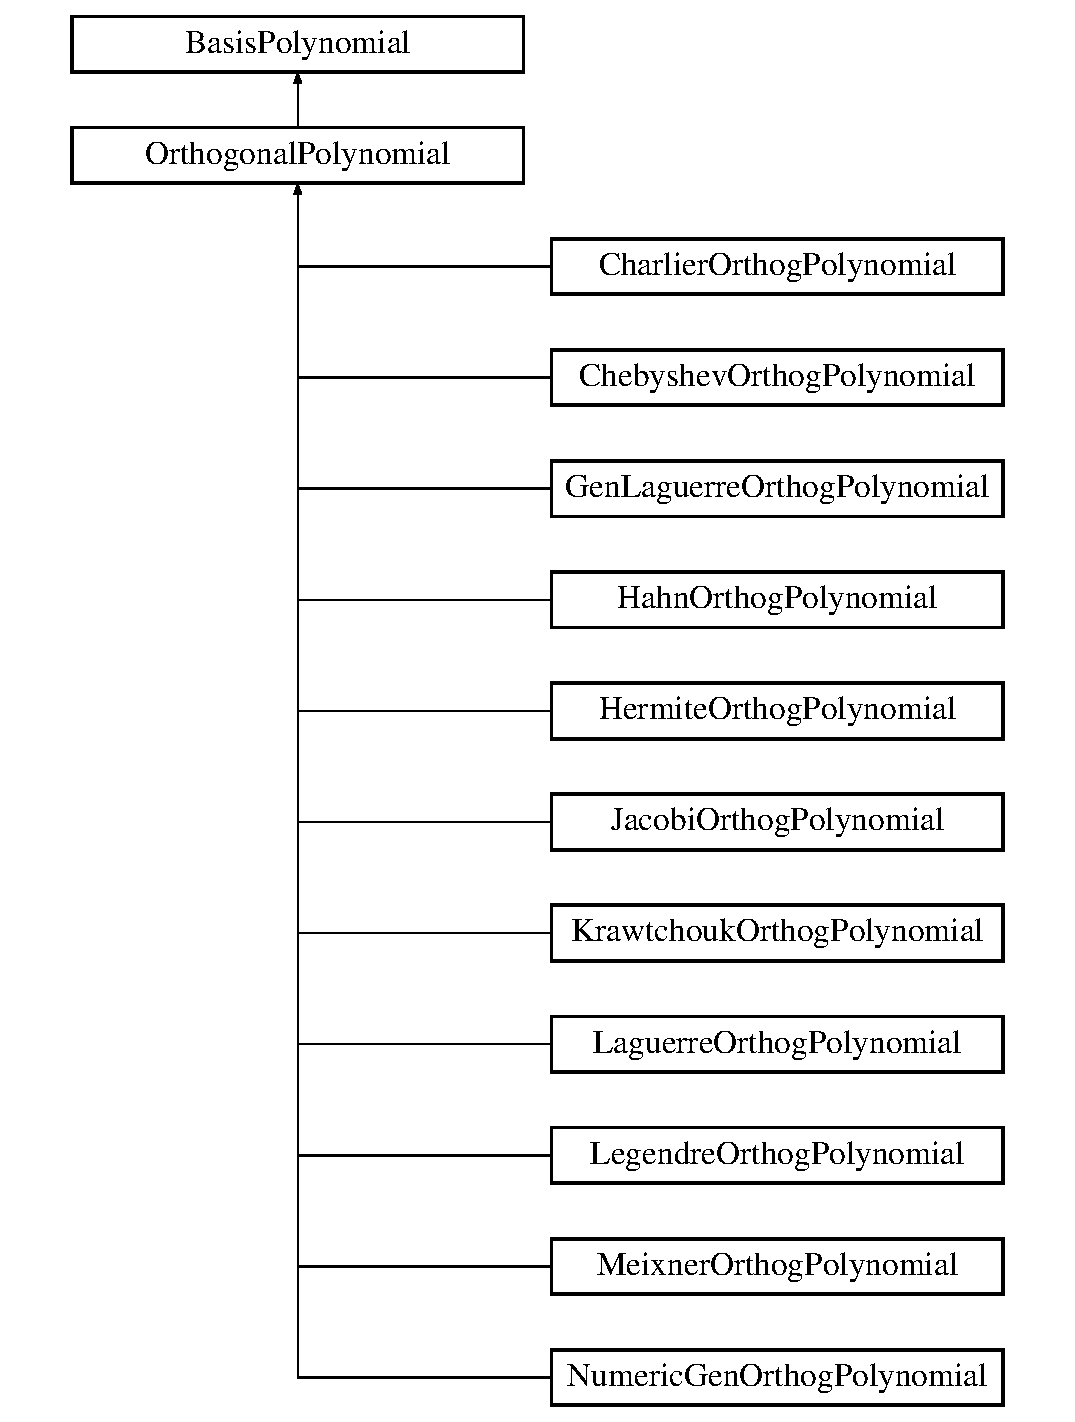
\includegraphics[height=12.000000cm]{classPecos_1_1OrthogonalPolynomial}
\end{center}
\end{figure}
\subsection*{Public Member Functions}
\begin{DoxyCompactItemize}
\item 
\hyperlink{classPecos_1_1OrthogonalPolynomial_a0547c9de695c718852fbac1852550226}{$\sim$\+Orthogonal\+Polynomial} ()\label{classPecos_1_1OrthogonalPolynomial_a0547c9de695c718852fbac1852550226}

\begin{DoxyCompactList}\small\item\em default constructor \end{DoxyCompactList}\item 
void \hyperlink{classPecos_1_1OrthogonalPolynomial_ad6115367af3811a5c75acbe340f04e58}{reset\+\_\+gauss} ()
\begin{DoxyCompactList}\small\item\em destructor \end{DoxyCompactList}\item 
void \hyperlink{classPecos_1_1OrthogonalPolynomial_ae0a12f67636f1a11987ed07e52d894b4}{precompute\+\_\+triple\+\_\+products} (const U\+Short\+Multi\+Set \&max\+\_\+ijk)
\begin{DoxyCompactList}\small\item\em precompute triple\+Product\+Map \end{DoxyCompactList}\item 
bool \hyperlink{classPecos_1_1OrthogonalPolynomial_ac922291ee984b86b16e4eba2109d7f03}{triple\+\_\+product} (const U\+Short\+Multi\+Set \&ijk\+\_\+key, Real \&trip\+\_\+prod) const \label{classPecos_1_1OrthogonalPolynomial_ac922291ee984b86b16e4eba2109d7f03}

\begin{DoxyCompactList}\small\item\em lookup value based on U\+Short\+Multi\+Set key within triple\+Product\+Map; returns false if not stored \end{DoxyCompactList}\item 
bool \hyperlink{classPecos_1_1OrthogonalPolynomial_acdf9ef648b8655a19be44b125e87a92f}{triple\+\_\+product} (size\+\_\+t i, size\+\_\+t j, size\+\_\+t k, Real \&trip\+\_\+prod) const \label{classPecos_1_1OrthogonalPolynomial_acdf9ef648b8655a19be44b125e87a92f}

\begin{DoxyCompactList}\small\item\em lookup value based on three size\+\_\+t keys within triple\+Product\+Map; returns false if not stored \end{DoxyCompactList}\item 
void \hyperlink{classPecos_1_1OrthogonalPolynomial_acef82563bd01f76a8c564664840de3fa}{gauss\+\_\+check} (unsigned short order)\label{classPecos_1_1OrthogonalPolynomial_acef82563bd01f76a8c564664840de3fa}

\begin{DoxyCompactList}\small\item\em perform unit testing on Gauss points/weights \end{DoxyCompactList}\end{DoxyCompactItemize}
\subsection*{Protected Member Functions}
\begin{DoxyCompactItemize}
\item 
void \hyperlink{classPecos_1_1OrthogonalPolynomial_addd13d4093ce8cbf2d22c47a47aff610}{collocation\+\_\+rule} (short rule)\label{classPecos_1_1OrthogonalPolynomial_addd13d4093ce8cbf2d22c47a47aff610}

\begin{DoxyCompactList}\small\item\em set colloc\+Rule \end{DoxyCompactList}\item 
short \hyperlink{classPecos_1_1OrthogonalPolynomial_a2e390f265fcc800348dc816d6cc37f86}{collocation\+\_\+rule} () const \label{classPecos_1_1OrthogonalPolynomial_a2e390f265fcc800348dc816d6cc37f86}

\begin{DoxyCompactList}\small\item\em get colloc\+Rule \end{DoxyCompactList}\end{DoxyCompactItemize}
\subsection*{Protected Attributes}
\begin{DoxyCompactItemize}
\item 
Real\+Array \hyperlink{classPecos_1_1OrthogonalPolynomial_abaca893e4d013e2d17107a007af07de0}{colloc\+Points}\label{classPecos_1_1OrthogonalPolynomial_abaca893e4d013e2d17107a007af07de0}

\begin{DoxyCompactList}\small\item\em collocation points for one-\/dimensional quadrature (x parameter values for which Poly\+\_\+n(x) = 0) \end{DoxyCompactList}\item 
Real\+Array \hyperlink{classPecos_1_1OrthogonalPolynomial_aa06828ef22dc2a16825fcdf6a873e0c9}{colloc\+Weights}\label{classPecos_1_1OrthogonalPolynomial_aa06828ef22dc2a16825fcdf6a873e0c9}

\begin{DoxyCompactList}\small\item\em collocation weights for one-\/dimensional quadrature \end{DoxyCompactList}\item 
short \hyperlink{classPecos_1_1OrthogonalPolynomial_abcc1d84cc8e8c8b5a66f720067039f2e}{colloc\+Rule}
\begin{DoxyCompactList}\small\item\em the type of integration rule associated with the orthogonal polynomial \end{DoxyCompactList}\end{DoxyCompactItemize}
\subsection*{Private Attributes}
\begin{DoxyCompactItemize}
\item 
U\+Short\+Multi\+Set\+Real\+Map \hyperlink{classPecos_1_1OrthogonalPolynomial_aece1e68316cdaf6be06745c62046c6ec}{triple\+Product\+Map}\label{classPecos_1_1OrthogonalPolynomial_aece1e68316cdaf6be06745c62046c6ec}

\begin{DoxyCompactList}\small\item\em mapping from an ijk sorted index set into $<$\+Psi\+\_\+i psi\+\_\+j=\char`\"{}\char`\"{} psi\+\_\+k$>$=\char`\"{}\char`\"{}$>$. These are precomputed with precompute\+\_\+triple\+\_\+products(order) and retrieved with triple\+\_\+product(key) \end{DoxyCompactList}\item 
U\+Short\+Multi\+Set \hyperlink{classPecos_1_1OrthogonalPolynomial_a22ebc8368302d88c43e62e9075f429d0}{triple\+Product\+Order}\label{classPecos_1_1OrthogonalPolynomial_a22ebc8368302d88c43e62e9075f429d0}

\begin{DoxyCompactList}\small\item\em tracks precomputations to prevent redundancy \end{DoxyCompactList}\end{DoxyCompactItemize}
\subsection*{Additional Inherited Members}


\subsection{Detailed Description}
Base class for the orthogonal polynomial class hierarchy. 

The \hyperlink{classPecos_1_1OrthogonalPolynomial}{Orthogonal\+Polynomial} class is the base class for the univariate orthogonal polynomial class hierarchy in P\+E\+C\+OS. One instance of an \hyperlink{classPecos_1_1OrthogonalPolynomial}{Orthogonal\+Polynomial} is created for each variable within a multidimensional orthogonal polynomial basis function (a vector of Orthogonal\+Polynomials is contained in \hyperlink{classPecos_1_1OrthogPolyApproximation}{Orthog\+Poly\+Approximation}, which may be mixed and matched in, e.\+g., the Wiener-\/\+Askey scheme for polynomial chaos). 

\subsection{Member Function Documentation}
\index{Pecos\+::\+Orthogonal\+Polynomial@{Pecos\+::\+Orthogonal\+Polynomial}!reset\+\_\+gauss@{reset\+\_\+gauss}}
\index{reset\+\_\+gauss@{reset\+\_\+gauss}!Pecos\+::\+Orthogonal\+Polynomial@{Pecos\+::\+Orthogonal\+Polynomial}}
\subsubsection[{\texorpdfstring{reset\+\_\+gauss()}{reset_gauss()}}]{\setlength{\rightskip}{0pt plus 5cm}void reset\+\_\+gauss (
\begin{DoxyParamCaption}
{}
\end{DoxyParamCaption}
)\hspace{0.3cm}{\ttfamily [inline]}, {\ttfamily [virtual]}}\label{classPecos_1_1OrthogonalPolynomial_ad6115367af3811a5c75acbe340f04e58}


destructor 

destroy history of Gauss pts/wts due to change in distribution parameters 

Reimplemented from \hyperlink{classPecos_1_1BasisPolynomial_ad6115367af3811a5c75acbe340f04e58}{Basis\+Polynomial}.



References Orthogonal\+Polynomial\+::colloc\+Points, Orthogonal\+Polynomial\+::colloc\+Weights, and Orthogonal\+Polynomial\+::triple\+\_\+product().



Referenced by Charlier\+Orthog\+Polynomial\+::alpha\+\_\+stat(), Krawtchouk\+Orthog\+Polynomial\+::alpha\+\_\+stat(), Meixner\+Orthog\+Polynomial\+::alpha\+\_\+stat(), Hahn\+Orthog\+Polynomial\+::alpha\+\_\+stat(), Gen\+Laguerre\+Orthog\+Polynomial\+::alpha\+\_\+stat(), Jacobi\+Orthog\+Polynomial\+::alpha\+\_\+stat(), Krawtchouk\+Orthog\+Polynomial\+::beta\+\_\+stat(), Meixner\+Orthog\+Polynomial\+::beta\+\_\+stat(), Hahn\+Orthog\+Polynomial\+::beta\+\_\+stat(), Jacobi\+Orthog\+Polynomial\+::beta\+\_\+stat(), Numeric\+Gen\+Orthog\+Polynomial\+::bounded\+\_\+lognormal\+\_\+distribution(), Numeric\+Gen\+Orthog\+Polynomial\+::bounded\+\_\+normal\+\_\+distribution(), Numeric\+Gen\+Orthog\+Polynomial\+::frechet\+\_\+distribution(), Hahn\+Orthog\+Polynomial\+::gamma\+\_\+stat(), Numeric\+Gen\+Orthog\+Polynomial\+::gumbel\+\_\+distribution(), Numeric\+Gen\+Orthog\+Polynomial\+::histogram\+\_\+bin\+\_\+distribution(), Numeric\+Gen\+Orthog\+Polynomial\+::histogram\+\_\+pt\+\_\+distribution(), Numeric\+Gen\+Orthog\+Polynomial\+::lognormal\+\_\+distribution(), Numeric\+Gen\+Orthog\+Polynomial\+::loguniform\+\_\+distribution(), Numeric\+Gen\+Orthog\+Polynomial\+::triangular\+\_\+distribution(), and Numeric\+Gen\+Orthog\+Polynomial\+::weibull\+\_\+distribution().

\index{Pecos\+::\+Orthogonal\+Polynomial@{Pecos\+::\+Orthogonal\+Polynomial}!precompute\+\_\+triple\+\_\+products@{precompute\+\_\+triple\+\_\+products}}
\index{precompute\+\_\+triple\+\_\+products@{precompute\+\_\+triple\+\_\+products}!Pecos\+::\+Orthogonal\+Polynomial@{Pecos\+::\+Orthogonal\+Polynomial}}
\subsubsection[{\texorpdfstring{precompute\+\_\+triple\+\_\+products(const U\+Short\+Multi\+Set \&max\+\_\+ijk)}{precompute_triple_products(const UShortMultiSet &max_ijk)}}]{\setlength{\rightskip}{0pt plus 5cm}void precompute\+\_\+triple\+\_\+products (
\begin{DoxyParamCaption}
\item[{const U\+Short\+Multi\+Set \&}]{max\+\_\+ijk}
\end{DoxyParamCaption}
)}\label{classPecos_1_1OrthogonalPolynomial_ae0a12f67636f1a11987ed07e52d894b4}


precompute triple\+Product\+Map 

There are a number of ways to do this precomputation. The P\+E\+C\+OS approach favors memory over flops by storing nonzero Cijk only for unique index sets. This approach requires a lookup of index sets rather than direct iteration over non-\/zeros. An alternative approach (used by Stokhos) that favors flops would store all non-\/zeros and return iterators to allow efficient iteration over these non-\/zeros. 

References Basis\+Polynomial\+::collocation\+\_\+points(), Orthogonal\+Polynomial\+::colloc\+Rule, Basis\+Polynomial\+::norm\+\_\+squared(), Orthogonal\+Polynomial\+::triple\+Product\+Map, Orthogonal\+Polynomial\+::triple\+Product\+Order, Basis\+Polynomial\+::type1\+\_\+collocation\+\_\+weights(), and Basis\+Polynomial\+::type1\+\_\+value().



Referenced by Orthogonal\+Polynomial\+::gauss\+\_\+check(), Orthog\+Poly\+Approximation\+::multiply\+\_\+expansion(), and Regress\+Orthog\+Poly\+Approximation\+::multiply\+\_\+expansion().



\subsection{Member Data Documentation}
\index{Pecos\+::\+Orthogonal\+Polynomial@{Pecos\+::\+Orthogonal\+Polynomial}!colloc\+Rule@{colloc\+Rule}}
\index{colloc\+Rule@{colloc\+Rule}!Pecos\+::\+Orthogonal\+Polynomial@{Pecos\+::\+Orthogonal\+Polynomial}}
\subsubsection[{\texorpdfstring{colloc\+Rule}{collocRule}}]{\setlength{\rightskip}{0pt plus 5cm}short colloc\+Rule\hspace{0.3cm}{\ttfamily [protected]}}\label{classPecos_1_1OrthogonalPolynomial_abcc1d84cc8e8c8b5a66f720067039f2e}


the type of integration rule associated with the orthogonal polynomial 

In most cases, this is just the corresponding Gauss quadrature rule. However, for Legendre, colloc\+Rule manages the option of G\+A\+U\+S\+S\+\_\+\+L\+E\+G\+E\+N\+D\+RE or G\+A\+U\+S\+S\+\_\+\+P\+A\+T\+T\+E\+R\+S\+ON, for Chebyshev, it manages the option of C\+L\+E\+N\+S\+H\+A\+W\+\_\+\+C\+U\+R\+T\+IS or F\+E\+J\+E\+R2, and for Hermite, it manages the option of G\+A\+U\+S\+S\+\_\+\+H\+E\+R\+M\+I\+TE or G\+E\+N\+Z\+\_\+\+K\+E\+I\+S\+T\+ER. 

Referenced by Chebyshev\+Orthog\+Polynomial\+::\+Chebyshev\+Orthog\+Polynomial(), Hermite\+Orthog\+Polynomial\+::collocation\+\_\+points(), Chebyshev\+Orthog\+Polynomial\+::collocation\+\_\+points(), Legendre\+Orthog\+Polynomial\+::collocation\+\_\+points(), Orthogonal\+Polynomial\+::collocation\+\_\+rule(), Gen\+Laguerre\+Orthog\+Polynomial\+::\+Gen\+Laguerre\+Orthog\+Polynomial(), Hermite\+Orthog\+Polynomial\+::\+Hermite\+Orthog\+Polynomial(), Jacobi\+Orthog\+Polynomial\+::\+Jacobi\+Orthog\+Polynomial(), Laguerre\+Orthog\+Polynomial\+::\+Laguerre\+Orthog\+Polynomial(), Legendre\+Orthog\+Polynomial\+::\+Legendre\+Orthog\+Polynomial(), Numeric\+Gen\+Orthog\+Polynomial\+::\+Numeric\+Gen\+Orthog\+Polynomial(), Orthogonal\+Polynomial\+::precompute\+\_\+triple\+\_\+products(), Chebyshev\+Orthog\+Polynomial\+::type1\+\_\+collocation\+\_\+weights(), Hermite\+Orthog\+Polynomial\+::type1\+\_\+collocation\+\_\+weights(), and Legendre\+Orthog\+Polynomial\+::type1\+\_\+collocation\+\_\+weights().



The documentation for this class was generated from the following files\+:\begin{DoxyCompactItemize}
\item 
Orthogonal\+Polynomial.\+hpp\item 
Orthogonal\+Polynomial.\+cpp\end{DoxyCompactItemize}

\section{Orthog\+Poly\+Approximation Class Reference}
\label{classPecos_1_1OrthogPolyApproximation}\index{Orthog\+Poly\+Approximation@{Orthog\+Poly\+Approximation}}


Derived approximation class for orthogonal polynomials (global approximation).  


Inheritance diagram for Orthog\+Poly\+Approximation\+:\begin{figure}[H]
\begin{center}
\leavevmode
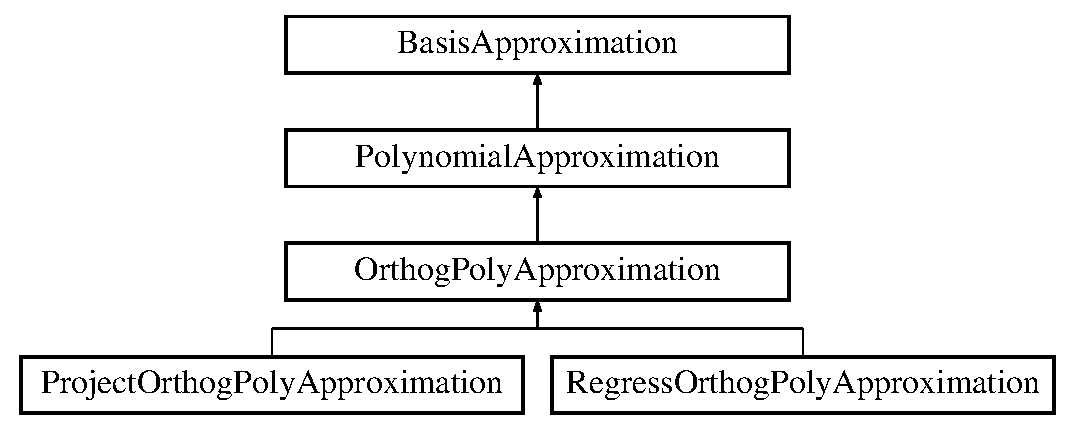
\includegraphics[height=4.000000cm]{classPecos_1_1OrthogPolyApproximation}
\end{center}
\end{figure}
\subsection*{Public Member Functions}
\begin{DoxyCompactItemize}
\item 
\hyperlink{classPecos_1_1OrthogPolyApproximation_ac035faa53ad34098ac86dbd6b71e65ee}{Orthog\+Poly\+Approximation} (const \hyperlink{classPecos_1_1SharedBasisApproxData}{Shared\+Basis\+Approx\+Data} \&shared\+\_\+data)\label{classPecos_1_1OrthogPolyApproximation_ac035faa53ad34098ac86dbd6b71e65ee}

\begin{DoxyCompactList}\small\item\em default constructor \end{DoxyCompactList}\item 
\hyperlink{classPecos_1_1OrthogPolyApproximation_a50dc870dba75b5030aeb9870e5e6aa3c}{$\sim$\+Orthog\+Poly\+Approximation} ()\label{classPecos_1_1OrthogPolyApproximation_a50dc870dba75b5030aeb9870e5e6aa3c}

\begin{DoxyCompactList}\small\item\em destructor \end{DoxyCompactList}\item 
virtual size\+\_\+t \hyperlink{classPecos_1_1OrthogPolyApproximation_a1472574cce875722141b69b4eb629572}{expansion\+\_\+terms} () const 
\begin{DoxyCompactList}\small\item\em retrieve number of terms in the orthogonal polynomial expansion \end{DoxyCompactList}\item 
virtual const Real\+Vector \& \hyperlink{classPecos_1_1OrthogPolyApproximation_af479d04cda6ec328a589f1b63ddb37eb}{dimension\+\_\+decay\+\_\+rates} ()\label{classPecos_1_1OrthogPolyApproximation_af479d04cda6ec328a589f1b63ddb37eb}

\begin{DoxyCompactList}\small\item\em estimate chaos expansion coefficient decay rates for each random variable dimension using linear least squares in semilog space \end{DoxyCompactList}\item 
void {\bfseries basis\+\_\+matrix} (const Real\+Matrix \&x, Real\+Matrix \&basis\+\_\+values)\label{classPecos_1_1OrthogPolyApproximation_ad7879e5a6e4cc3acfd6e26cb25edefde}

\end{DoxyCompactItemize}
\subsection*{Static Public Member Functions}
\begin{DoxyCompactItemize}
\item 
static void \hyperlink{classPecos_1_1OrthogPolyApproximation_a737da4973b81df7d2f3f035bde58e4e7}{basis\+\_\+value} (const Real\+Vector \&x, std\+::vector$<$ \hyperlink{classPecos_1_1BasisPolynomial}{Basis\+Polynomial} $>$ \&polynomial\+\_\+basis, const U\+Short2\+D\+Array \&multi\+\_\+index, Real\+Vector \&basis\+\_\+values)\label{classPecos_1_1OrthogPolyApproximation_a737da4973b81df7d2f3f035bde58e4e7}

\begin{DoxyCompactList}\small\item\em evaluate all pce basis functions at a single point \end{DoxyCompactList}\item 
static void \hyperlink{classPecos_1_1OrthogPolyApproximation_a9e7918f42d9c8b52624750ee4882495e}{basis\+\_\+matrix} (const Real\+Matrix \&x, std\+::vector$<$ \hyperlink{classPecos_1_1BasisPolynomial}{Basis\+Polynomial} $>$ \&polynomial\+\_\+basis, const U\+Short2\+D\+Array \&multi\+\_\+index, Real\+Matrix \&basis\+\_\+values)\label{classPecos_1_1OrthogPolyApproximation_a9e7918f42d9c8b52624750ee4882495e}

\begin{DoxyCompactList}\small\item\em evaluate all pce basis functions at a set of points \end{DoxyCompactList}\end{DoxyCompactItemize}
\subsection*{Protected Member Functions}
\begin{DoxyCompactItemize}
\item 
int \hyperlink{classPecos_1_1OrthogPolyApproximation_ac789358ee49633613d6c97593be06f9d}{min\+\_\+coefficients} () const \label{classPecos_1_1OrthogPolyApproximation_ac789358ee49633613d6c97593be06f9d}

\begin{DoxyCompactList}\small\item\em return the minimum number of samples (unknowns) required to build the derived class approximation type in num\+Vars dimensions \end{DoxyCompactList}\item 
void \hyperlink{classPecos_1_1OrthogPolyApproximation_abc17a7104c33d8146f4a0ee7b6c6f37a}{store\+\_\+coefficients} (size\+\_\+t index=\+\_\+\+N\+P\+OS)\label{classPecos_1_1OrthogPolyApproximation_abc17a7104c33d8146f4a0ee7b6c6f37a}

\begin{DoxyCompactList}\small\item\em store the current coefficients for later combination \end{DoxyCompactList}\item 
void \hyperlink{classPecos_1_1OrthogPolyApproximation_ad05b093ee96314c9e05bad8e06c2dae7}{restore\+\_\+coefficients} (size\+\_\+t index=\+\_\+\+N\+P\+OS)\label{classPecos_1_1OrthogPolyApproximation_ad05b093ee96314c9e05bad8e06c2dae7}

\begin{DoxyCompactList}\small\item\em restore a previously stored coefficient state \end{DoxyCompactList}\item 
void \hyperlink{classPecos_1_1OrthogPolyApproximation_a859795ba714d81e821bec254479135ee}{swap\+\_\+coefficients} (size\+\_\+t maximal\+\_\+index)\label{classPecos_1_1OrthogPolyApproximation_a859795ba714d81e821bec254479135ee}

\begin{DoxyCompactList}\small\item\em swap the current coefficients with a previously stored set \end{DoxyCompactList}\item 
void \hyperlink{classPecos_1_1OrthogPolyApproximation_a63d12cc6021fda4896b8738d72dfcc86}{remove\+\_\+stored\+\_\+coefficients} (size\+\_\+t index=\+\_\+\+N\+P\+OS)\label{classPecos_1_1OrthogPolyApproximation_a63d12cc6021fda4896b8738d72dfcc86}

\begin{DoxyCompactList}\small\item\em remove a redundant stored entry prior to combine\+\_\+coefficients (default is pop\+\_\+back) \end{DoxyCompactList}\item 
void \hyperlink{classPecos_1_1OrthogPolyApproximation_ae4337960917eda26a5672e5c6afbb62a}{clear\+\_\+stored} ()\label{classPecos_1_1OrthogPolyApproximation_ae4337960917eda26a5672e5c6afbb62a}

\begin{DoxyCompactList}\small\item\em clear stored approximation data \end{DoxyCompactList}\item 
void \hyperlink{classPecos_1_1OrthogPolyApproximation_a7c794213befc83c9f90137f22e4cd39d}{combine\+\_\+coefficients} (size\+\_\+t swap\+\_\+index)\label{classPecos_1_1OrthogPolyApproximation_a7c794213befc83c9f90137f22e4cd39d}

\begin{DoxyCompactList}\small\item\em combine the current coefficients with a previously stored set \end{DoxyCompactList}\item 
void \hyperlink{classPecos_1_1OrthogPolyApproximation_a4beb4a3300443171ac2233e87c970e39}{print\+\_\+coefficients} (std\+::ostream \&s, bool normalized)\label{classPecos_1_1OrthogPolyApproximation_a4beb4a3300443171ac2233e87c970e39}

\begin{DoxyCompactList}\small\item\em print the coefficient array computed in \hyperlink{classPecos_1_1PolynomialApproximation_aef8f0c32bdeff7756a9c614607c03058}{compute\+\_\+coefficients()} \end{DoxyCompactList}\item 
Real\+Vector \hyperlink{classPecos_1_1OrthogPolyApproximation_ac64f16ff9fbfb80c4bafa969b4a92e1d}{approximation\+\_\+coefficients} (bool normalized) const \label{classPecos_1_1OrthogPolyApproximation_ac64f16ff9fbfb80c4bafa969b4a92e1d}

\begin{DoxyCompactList}\small\item\em retrieve or form a set of dense coefficients that correspond to \hyperlink{classPecos_1_1SharedOrthogPolyApproxData_a0fbdd5817bc6dd026f6d42269ca8e703}{Shared\+Orthog\+Poly\+Approx\+Data\+::multi\+Index} \end{DoxyCompactList}\item 
void \hyperlink{classPecos_1_1OrthogPolyApproximation_a2e7b82322962df3fd036b9e0783d8fc9}{approximation\+\_\+coefficients} (const Real\+Vector \&approx\+\_\+coeffs, bool normalized)\label{classPecos_1_1OrthogPolyApproximation_a2e7b82322962df3fd036b9e0783d8fc9}

\begin{DoxyCompactList}\small\item\em set an array of dense coefficients corresponding to \hyperlink{classPecos_1_1SharedOrthogPolyApproxData_a0fbdd5817bc6dd026f6d42269ca8e703}{Shared\+Orthog\+Poly\+Approx\+Data\+::multi\+Index} \end{DoxyCompactList}\item 
void \hyperlink{classPecos_1_1OrthogPolyApproximation_acbb94332d149ea052464dac73321ddcf}{coefficient\+\_\+labels} (std\+::vector$<$ std\+::string $>$ \&all\+\_\+coeff\+\_\+tags) const \label{classPecos_1_1OrthogPolyApproximation_acbb94332d149ea052464dac73321ddcf}

\begin{DoxyCompactList}\small\item\em retrieve a vector of coefficient label strings, one per expansion term \end{DoxyCompactList}\item 
void \hyperlink{classPecos_1_1OrthogPolyApproximation_a37ef37829b412fefa40d53b395846781}{allocate\+\_\+arrays} ()\label{classPecos_1_1OrthogPolyApproximation_a37ef37829b412fefa40d53b395846781}

\begin{DoxyCompactList}\small\item\em initialize multi\+Index, expansion\+Coeffs, et al. \end{DoxyCompactList}\item 
void \hyperlink{classPecos_1_1OrthogPolyApproximation_abec3f45a112004b53f83b3a03e0d06db}{compute\+\_\+component\+\_\+sobol} ()\label{classPecos_1_1OrthogPolyApproximation_abec3f45a112004b53f83b3a03e0d06db}

\begin{DoxyCompactList}\small\item\em Performs global sensitivity analysis via variance-\/based decomposition; computes component (main and interaction) Sobol\textquotesingle{} indices. \end{DoxyCompactList}\item 
void \hyperlink{classPecos_1_1OrthogPolyApproximation_ada0deadfa2c3202ed4e58d066ee079f2}{compute\+\_\+total\+\_\+sobol} ()\label{classPecos_1_1OrthogPolyApproximation_ada0deadfa2c3202ed4e58d066ee079f2}

\begin{DoxyCompactList}\small\item\em Performs global sensitivity analysis via variance-\/based decomposition; computes total Sobol\textquotesingle{} indices. \end{DoxyCompactList}\item 
Real \hyperlink{classPecos_1_1OrthogPolyApproximation_a7bc9dcdf32fc46f97e286268c1ac51b0}{value} (const Real\+Vector \&x)\label{classPecos_1_1OrthogPolyApproximation_a7bc9dcdf32fc46f97e286268c1ac51b0}

\begin{DoxyCompactList}\small\item\em retrieve the approximate function value for a given parameter vector \end{DoxyCompactList}\item 
const Real\+Vector \& \hyperlink{classPecos_1_1OrthogPolyApproximation_ae3b6ea541392b74cf0cc8758e206277c}{gradient\+\_\+basis\+\_\+variables} (const Real\+Vector \&x)\label{classPecos_1_1OrthogPolyApproximation_ae3b6ea541392b74cf0cc8758e206277c}

\begin{DoxyCompactList}\small\item\em retrieve the gradient for a response expansion with respect to all variables included in the polynomial bases using the given parameter vector and default D\+VV \end{DoxyCompactList}\item 
const Real\+Vector \& \hyperlink{classPecos_1_1OrthogPolyApproximation_a3ffb563ae1658344bfc2ad882def9e7c}{gradient\+\_\+basis\+\_\+variables} (const Real\+Vector \&x, const Sizet\+Array \&dvv)\label{classPecos_1_1OrthogPolyApproximation_a3ffb563ae1658344bfc2ad882def9e7c}

\begin{DoxyCompactList}\small\item\em retrieve the gradient for a response expansion with respect to variables included in the polynomial basis for a given parameter vector and a given D\+VV subset \end{DoxyCompactList}\item 
const Real\+Vector \& \hyperlink{classPecos_1_1OrthogPolyApproximation_a518e8604f973a4b161a9b5718a0aa25e}{gradient\+\_\+nonbasis\+\_\+variables} (const Real\+Vector \&x)\label{classPecos_1_1OrthogPolyApproximation_a518e8604f973a4b161a9b5718a0aa25e}

\begin{DoxyCompactList}\small\item\em retrieve the gradient for a response expansion with respect to all variables not included in the polynomial bases (nonprobabilistic variables such as design or epistemic when not in \char`\"{}all\char`\"{} mode) using the given parameter vector and default D\+VV \end{DoxyCompactList}\item 
const Real\+Sym\+Matrix \& \hyperlink{classPecos_1_1OrthogPolyApproximation_a830729654265d84af637960f8c63f2bc}{hessian\+\_\+basis\+\_\+variables} (const Real\+Vector \&x)\label{classPecos_1_1OrthogPolyApproximation_a830729654265d84af637960f8c63f2bc}

\begin{DoxyCompactList}\small\item\em retrieve the Hessian of the response expansion with respect to all variables included in the polynomial basis (e.\+g., probabilistic variables) for a given parameter vector \end{DoxyCompactList}\item 
Real \hyperlink{classPecos_1_1OrthogPolyApproximation_a1abe918dbdc66ac0fde85f1ab3c061af}{stored\+\_\+value} (const Real\+Vector \&x, size\+\_\+t index)\label{classPecos_1_1OrthogPolyApproximation_a1abe918dbdc66ac0fde85f1ab3c061af}

\begin{DoxyCompactList}\small\item\em retrieve the response value for a stored expansion using the given parameter vector \end{DoxyCompactList}\item 
const Real\+Vector \& \hyperlink{classPecos_1_1OrthogPolyApproximation_a7689fc058e2efdde6ce4dfe898864592}{stored\+\_\+gradient\+\_\+basis\+\_\+variables} (const Real\+Vector \&x, size\+\_\+t index)\label{classPecos_1_1OrthogPolyApproximation_a7689fc058e2efdde6ce4dfe898864592}

\begin{DoxyCompactList}\small\item\em retrieve the response gradient for a stored expansion with respect to all variables included in the polynomial bases; evaluate for the given parameter vector. \end{DoxyCompactList}\item 
const Real\+Vector \& \hyperlink{classPecos_1_1OrthogPolyApproximation_af0c9184d9a0da7b0e3d0d3ecbfc8f434}{stored\+\_\+gradient\+\_\+nonbasis\+\_\+variables} (const Real\+Vector \&x, size\+\_\+t index)\label{classPecos_1_1OrthogPolyApproximation_af0c9184d9a0da7b0e3d0d3ecbfc8f434}

\begin{DoxyCompactList}\small\item\em retrieve the response gradient for a stored expansion with respect to all variables not included in the polynomial bases; evaluate for the given parameter vector. \end{DoxyCompactList}\item 
Real \hyperlink{classPecos_1_1OrthogPolyApproximation_adc6f262952d05a33ff68cae37929cbb2}{mean} ()
\item 
Real \hyperlink{classPecos_1_1OrthogPolyApproximation_aed107df248a4555c052446fbc10a8e61}{mean} (const Real\+Vector \&x)
\item 
const Real\+Vector \& \hyperlink{classPecos_1_1OrthogPolyApproximation_a069c87a26fdb4b09af68db26abd646a0}{mean\+\_\+gradient} ()
\item 
const Real\+Vector \& \hyperlink{classPecos_1_1OrthogPolyApproximation_a24f2edc21c9887121cda78faae1c1475}{mean\+\_\+gradient} (const Real\+Vector \&x, const Sizet\+Array \&dvv)
\item 
Real \hyperlink{classPecos_1_1OrthogPolyApproximation_a38f6da77468be17e02ce38af2c0976c3}{variance} ()
\item 
Real \hyperlink{classPecos_1_1OrthogPolyApproximation_acbdcb523a161d7d3a5cc190796e84ede}{variance} (const Real\+Vector \&x)
\item 
const Real\+Vector \& \hyperlink{classPecos_1_1OrthogPolyApproximation_ae898fc2f42f1077268f89fc2e9f2c71c}{variance\+\_\+gradient} ()
\item 
const Real\+Vector \& \hyperlink{classPecos_1_1OrthogPolyApproximation_a791e127a445f8a6c9c3a7966d12c1431}{variance\+\_\+gradient} (const Real\+Vector \&x, const Sizet\+Array \&dvv)
\item 
Real \hyperlink{classPecos_1_1OrthogPolyApproximation_ac0085912d4abb9caa3f480b9c6778c0e}{covariance} (\hyperlink{classPecos_1_1PolynomialApproximation}{Polynomial\+Approximation} $\ast$poly\+\_\+approx\+\_\+2)\label{classPecos_1_1OrthogPolyApproximation_ac0085912d4abb9caa3f480b9c6778c0e}

\begin{DoxyCompactList}\small\item\em return the covariance between two response expansions, treating all variables as random \end{DoxyCompactList}\item 
Real \hyperlink{classPecos_1_1OrthogPolyApproximation_afc1731a3d89818d49c03a3c20a7a2898}{covariance} (const Real\+Vector \&x, \hyperlink{classPecos_1_1PolynomialApproximation}{Polynomial\+Approximation} $\ast$poly\+\_\+approx\+\_\+2)\label{classPecos_1_1OrthogPolyApproximation_afc1731a3d89818d49c03a3c20a7a2898}

\begin{DoxyCompactList}\small\item\em return the covariance between two response expansions for a given parameter vector, treating a subset of the variables as random \end{DoxyCompactList}\item 
void \hyperlink{classPecos_1_1OrthogPolyApproximation_a5926c67431b0fc223fcfa6c11cb9de14}{compute\+\_\+moments} (bool full\+\_\+stats=true)\label{classPecos_1_1OrthogPolyApproximation_a5926c67431b0fc223fcfa6c11cb9de14}

\begin{DoxyCompactList}\small\item\em compute expansion moments to order 2 \end{DoxyCompactList}\item 
void \hyperlink{classPecos_1_1OrthogPolyApproximation_a2a6098ab4416bdcfdeadea5d46aa5f52}{compute\+\_\+moments} (const Real\+Vector \&x, bool full\+\_\+stats=true)\label{classPecos_1_1OrthogPolyApproximation_a2a6098ab4416bdcfdeadea5d46aa5f52}

\begin{DoxyCompactList}\small\item\em compute expansion moments in all-\/variables mode to order 2 \end{DoxyCompactList}\item 
void \hyperlink{classPecos_1_1OrthogPolyApproximation_a425685016976e6863c98b837883fa038}{size\+\_\+expansion} ()\label{classPecos_1_1OrthogPolyApproximation_a425685016976e6863c98b837883fa038}

\begin{DoxyCompactList}\small\item\em size expansion\{Coeffs,Coeff\+Grads\} based on multi\+Index \end{DoxyCompactList}\item 
void \hyperlink{classPecos_1_1OrthogPolyApproximation_a276dc60aec886932d86fd04e9698b63e}{size\+\_\+expansion} (size\+\_\+t num\+\_\+exp\+\_\+terms)\label{classPecos_1_1OrthogPolyApproximation_a276dc60aec886932d86fd04e9698b63e}

\begin{DoxyCompactList}\small\item\em size expansion\{Coeffs,Coeff\+Grads\} based on multi\+Index \end{DoxyCompactList}\item 
void \hyperlink{classPecos_1_1OrthogPolyApproximation_a9f739bb549630d4cc9ab914a17e16bd2}{resize\+\_\+expansion} ()\label{classPecos_1_1OrthogPolyApproximation_a9f739bb549630d4cc9ab914a17e16bd2}

\begin{DoxyCompactList}\small\item\em synchronize expansion\{Coeffs,Coeff\+Grads\} with an updated multi\+Index \end{DoxyCompactList}\item 
void \hyperlink{classPecos_1_1OrthogPolyApproximation_a5a7788b54991f0fa67d94eab7e9ef2a4}{resize\+\_\+expansion} (size\+\_\+t num\+\_\+exp\+\_\+terms)\label{classPecos_1_1OrthogPolyApproximation_a5a7788b54991f0fa67d94eab7e9ef2a4}

\begin{DoxyCompactList}\small\item\em synchronize expansion\{Coeffs,Coeff\+Grads\} with an updated multi\+Index \end{DoxyCompactList}\item 
void \hyperlink{classPecos_1_1OrthogPolyApproximation_a13c9bb4f0e799548d14f99a386bd34bb}{overlay\+\_\+expansion} (const Sizet\+Array \&multi\+\_\+index\+\_\+map, const Real\+Vector \&exp\+\_\+coeffs, const Real\+Matrix \&exp\+\_\+grads, int coeff)\label{classPecos_1_1OrthogPolyApproximation_a13c9bb4f0e799548d14f99a386bd34bb}

\begin{DoxyCompactList}\small\item\em overlay the passed expansion with the aggregate expansion\{Coeffs,Coeff\+Grads\} as managed by the multi\+\_\+index\+\_\+map \end{DoxyCompactList}\item 
void \hyperlink{classPecos_1_1OrthogPolyApproximation_ac55b330e5744fa8285ccae30dc691b13}{multiply\+\_\+expansion} (const U\+Short2\+D\+Array \&multi\+\_\+index\+\_\+b, const Real\+Vector \&exp\+\_\+coeffs\+\_\+b, const Real\+Matrix \&exp\+\_\+grads\+\_\+b, const U\+Short2\+D\+Array \&multi\+\_\+index\+\_\+c)\label{classPecos_1_1OrthogPolyApproximation_ac55b330e5744fa8285ccae30dc691b13}

\begin{DoxyCompactList}\small\item\em multiply current expansion (\char`\"{}a\char`\"{}) with incoming expansion (\char`\"{}b\char`\"{}) and store in product expansion (\char`\"{}c\char`\"{}) \end{DoxyCompactList}\item 
void \hyperlink{classPecos_1_1OrthogPolyApproximation_af98a9d8fd7b1b89052ce747c0ef483e4}{fail\+\_\+booleans} (Sizet\+Short\+Map\+::const\+\_\+iterator \&fit, size\+\_\+t j, bool \&add\+\_\+val, bool \&add\+\_\+grad)\label{classPecos_1_1OrthogPolyApproximation_af98a9d8fd7b1b89052ce747c0ef483e4}

\begin{DoxyCompactList}\small\item\em update add\+\_\+val and add\+\_\+gradient based on surr\+Data\textquotesingle{}s failure map \end{DoxyCompactList}\item 
void \hyperlink{classPecos_1_1OrthogPolyApproximation_a058505591316662aceef75a581e99db1}{integration\+\_\+checks} ()\label{classPecos_1_1OrthogPolyApproximation_a058505591316662aceef75a581e99db1}

\begin{DoxyCompactList}\small\item\em perform sanity checks prior to numerical integration \end{DoxyCompactList}\item 
void \hyperlink{classPecos_1_1OrthogPolyApproximation_ac321b5b2615931ac6032fc11521f58dd}{solve\+\_\+decay\+\_\+rates} (Real\+Vector\+Array \&A\+\_\+vectors, Real\+Vector\+Array \&b\+\_\+vectors, U\+Short\+Array \&max\+\_\+orders)\label{classPecos_1_1OrthogPolyApproximation_ac321b5b2615931ac6032fc11521f58dd}

\begin{DoxyCompactList}\small\item\em utility function for solving the least squares estimation of decay rates \end{DoxyCompactList}\end{DoxyCompactItemize}
\subsection*{Protected Attributes}
\begin{DoxyCompactItemize}
\item 
Real\+Vector \hyperlink{classPecos_1_1OrthogPolyApproximation_a2f49361bc93de38b3804a32d14ec9da2}{expansion\+Coeffs}\label{classPecos_1_1OrthogPolyApproximation_a2f49361bc93de38b3804a32d14ec9da2}

\begin{DoxyCompactList}\small\item\em the coefficients of the expansion \end{DoxyCompactList}\item 
Real\+Matrix \hyperlink{classPecos_1_1OrthogPolyApproximation_aafa9e6fb757964c3ce070ae4f980b6af}{expansion\+Coeff\+Grads}
\begin{DoxyCompactList}\small\item\em the gradients of the expansion coefficients \end{DoxyCompactList}\item 
Real\+Vector\+Array \hyperlink{classPecos_1_1OrthogPolyApproximation_a644b1a5bba418a7f83d3222881eb701d}{stored\+Exp\+Coeffs}\label{classPecos_1_1OrthogPolyApproximation_a644b1a5bba418a7f83d3222881eb701d}

\begin{DoxyCompactList}\small\item\em copies of expansion\+Coeffs stored in \hyperlink{classPecos_1_1OrthogPolyApproximation_abc17a7104c33d8146f4a0ee7b6c6f37a}{store\+\_\+coefficients()} for use in \hyperlink{classPecos_1_1OrthogPolyApproximation_a7c794213befc83c9f90137f22e4cd39d}{combine\+\_\+coefficients()} \end{DoxyCompactList}\item 
Real\+Matrix\+Array \hyperlink{classPecos_1_1OrthogPolyApproximation_acbc4f397b56c437fd8c956c59ae081d8}{stored\+Exp\+Coeff\+Grads}\label{classPecos_1_1OrthogPolyApproximation_acbc4f397b56c437fd8c956c59ae081d8}

\begin{DoxyCompactList}\small\item\em copies of expansion\+Coeff\+Grads stored in \hyperlink{classPecos_1_1OrthogPolyApproximation_abc17a7104c33d8146f4a0ee7b6c6f37a}{store\+\_\+coefficients()} for use in \hyperlink{classPecos_1_1OrthogPolyApproximation_a7c794213befc83c9f90137f22e4cd39d}{combine\+\_\+coefficients()} \end{DoxyCompactList}\item 
Real\+Vector \hyperlink{classPecos_1_1OrthogPolyApproximation_a4dff847cf479b3d67e81aec3937c9935}{decay\+Rates}\label{classPecos_1_1OrthogPolyApproximation_a4dff847cf479b3d67e81aec3937c9935}

\begin{DoxyCompactList}\small\item\em spectral coefficient decay rates estimated by L\+LS on log of univariate expansion coefficients \end{DoxyCompactList}\end{DoxyCompactItemize}
\subsection*{Private Member Functions}
\begin{DoxyCompactItemize}
\item 
void {\bfseries normalize} (const Real\+Vector \&std\+\_\+coeffs, Real\+Vector \&normalized\+\_\+coeffs) const \label{classPecos_1_1OrthogPolyApproximation_a8a62e62c51b185aa0cfe519a560ea413}

\item 
void {\bfseries denormalize} (const Real\+Vector \&normalized\+\_\+coeffs, Real\+Vector \&std\+\_\+coeffs) const \label{classPecos_1_1OrthogPolyApproximation_a6c3eb9538c7d44af423d8af4660364d6}

\end{DoxyCompactItemize}


\subsection{Detailed Description}
Derived approximation class for orthogonal polynomials (global approximation). 

The \hyperlink{classPecos_1_1OrthogPolyApproximation}{Orthog\+Poly\+Approximation} class provides a global approximation based on orthogonal polynomials. It is used primarily for polynomial chaos expansions (for stochastic finite element approaches to uncertainty quantification). 

\subsection{Member Function Documentation}
\index{Pecos\+::\+Orthog\+Poly\+Approximation@{Pecos\+::\+Orthog\+Poly\+Approximation}!expansion\+\_\+terms@{expansion\+\_\+terms}}
\index{expansion\+\_\+terms@{expansion\+\_\+terms}!Pecos\+::\+Orthog\+Poly\+Approximation@{Pecos\+::\+Orthog\+Poly\+Approximation}}
\subsubsection[{\texorpdfstring{expansion\+\_\+terms() const }{expansion_terms() const }}]{\setlength{\rightskip}{0pt plus 5cm}size\+\_\+t expansion\+\_\+terms (
\begin{DoxyParamCaption}
{}
\end{DoxyParamCaption}
) const\hspace{0.3cm}{\ttfamily [inline]}, {\ttfamily [virtual]}}\label{classPecos_1_1OrthogPolyApproximation_a1472574cce875722141b69b4eb629572}


retrieve number of terms in the orthogonal polynomial expansion 

default implementation if no sparsity (overridden in \hyperlink{classPecos_1_1RegressOrthogPolyApproximation}{Regress\+Orthog\+Poly\+Approximation} for CS) 

Reimplemented in \hyperlink{classPecos_1_1RegressOrthogPolyApproximation_a1472574cce875722141b69b4eb629572}{Regress\+Orthog\+Poly\+Approximation}.



References Shared\+Orthog\+Poly\+Approx\+Data\+::multi\+Index, and Basis\+Approximation\+::shared\+Data\+Rep.



Referenced by Regress\+Orthog\+Poly\+Approximation\+::expansion\+\_\+terms(), Orthog\+Poly\+Approximation\+::resize\+\_\+expansion(), and Orthog\+Poly\+Approximation\+::size\+\_\+expansion().

\index{Pecos\+::\+Orthog\+Poly\+Approximation@{Pecos\+::\+Orthog\+Poly\+Approximation}!mean@{mean}}
\index{mean@{mean}!Pecos\+::\+Orthog\+Poly\+Approximation@{Pecos\+::\+Orthog\+Poly\+Approximation}}
\subsubsection[{\texorpdfstring{mean()}{mean()}}]{\setlength{\rightskip}{0pt plus 5cm}Real mean (
\begin{DoxyParamCaption}
{}
\end{DoxyParamCaption}
)\hspace{0.3cm}{\ttfamily [protected]}, {\ttfamily [virtual]}}\label{classPecos_1_1OrthogPolyApproximation_adc6f262952d05a33ff68cae37929cbb2}
In this case, all expansion variables are random variables and the mean of the expansion is simply the first chaos coefficient. 

Implements \hyperlink{classPecos_1_1PolynomialApproximation_ae748f0525197363b2279cd36511fb791}{Polynomial\+Approximation}.



References Polynomial\+Approximation\+::computed\+Mean, Polynomial\+Approximation\+::expansion\+Coeff\+Flag, Orthog\+Poly\+Approximation\+::expansion\+Coeffs, Polynomial\+Approximation\+::expansion\+Moments, Shared\+Poly\+Approx\+Data\+::non\+Random\+Indices, and Basis\+Approximation\+::shared\+Data\+Rep.



Referenced by Project\+Orthog\+Poly\+Approximation\+::compute\+\_\+moments(), Orthog\+Poly\+Approximation\+::compute\+\_\+moments(), Project\+Orthog\+Poly\+Approximation\+::expectation(), Regress\+Orthog\+Poly\+Approximation\+::mean(), and Orthog\+Poly\+Approximation\+::mean().

\index{Pecos\+::\+Orthog\+Poly\+Approximation@{Pecos\+::\+Orthog\+Poly\+Approximation}!mean@{mean}}
\index{mean@{mean}!Pecos\+::\+Orthog\+Poly\+Approximation@{Pecos\+::\+Orthog\+Poly\+Approximation}}
\subsubsection[{\texorpdfstring{mean(const Real\+Vector \&x)}{mean(const RealVector &x)}}]{\setlength{\rightskip}{0pt plus 5cm}Real mean (
\begin{DoxyParamCaption}
\item[{const Real\+Vector \&}]{x}
\end{DoxyParamCaption}
)\hspace{0.3cm}{\ttfamily [protected]}, {\ttfamily [virtual]}}\label{classPecos_1_1OrthogPolyApproximation_aed107df248a4555c052446fbc10a8e61}
In this case, a subset of the expansion variables are random variables and the mean of the expansion involves evaluating the expectation over this subset. 

Implements \hyperlink{classPecos_1_1PolynomialApproximation_a69da68e2a4dd4b51439150ebfe4dc239}{Polynomial\+Approximation}.



Reimplemented in \hyperlink{classPecos_1_1RegressOrthogPolyApproximation_aed107df248a4555c052446fbc10a8e61}{Regress\+Orthog\+Poly\+Approximation}.



References Polynomial\+Approximation\+::computed\+Mean, Polynomial\+Approximation\+::expansion\+Coeff\+Flag, Orthog\+Poly\+Approximation\+::expansion\+Coeffs, Polynomial\+Approximation\+::expansion\+Moments, Shared\+Poly\+Approx\+Data\+::match\+\_\+nonrandom\+\_\+vars(), Orthog\+Poly\+Approximation\+::mean(), Shared\+Orthog\+Poly\+Approx\+Data\+::multi\+Index, Shared\+Orthog\+Poly\+Approx\+Data\+::multivariate\+\_\+polynomial(), Shared\+Poly\+Approx\+Data\+::non\+Random\+Indices, Basis\+Approximation\+::shared\+Data\+Rep, Polynomial\+Approximation\+::x\+Prev\+Mean, and Shared\+Orthog\+Poly\+Approx\+Data\+::zero\+\_\+random().

\index{Pecos\+::\+Orthog\+Poly\+Approximation@{Pecos\+::\+Orthog\+Poly\+Approximation}!mean\+\_\+gradient@{mean\+\_\+gradient}}
\index{mean\+\_\+gradient@{mean\+\_\+gradient}!Pecos\+::\+Orthog\+Poly\+Approximation@{Pecos\+::\+Orthog\+Poly\+Approximation}}
\subsubsection[{\texorpdfstring{mean\+\_\+gradient()}{mean_gradient()}}]{\setlength{\rightskip}{0pt plus 5cm}const Real\+Vector \& mean\+\_\+gradient (
\begin{DoxyParamCaption}
{}
\end{DoxyParamCaption}
)\hspace{0.3cm}{\ttfamily [protected]}, {\ttfamily [virtual]}}\label{classPecos_1_1OrthogPolyApproximation_a069c87a26fdb4b09af68db26abd646a0}
In this function, all expansion variables are random variables and any design/state variables are omitted from the expansion. In this case, the derivative of the expectation is the expectation of the derivative. The mixed derivative case (some design variables are inserted and some are augmented) requires no special treatment. 

Implements \hyperlink{classPecos_1_1PolynomialApproximation_abcb01df2fc2d4c44bab6b56ad7def50c}{Polynomial\+Approximation}.



References Polynomial\+Approximation\+::computed\+Mean, Polynomial\+Approximation\+::expansion\+Coeff\+Grad\+Flag, Orthog\+Poly\+Approximation\+::expansion\+Coeff\+Grads, Polynomial\+Approximation\+::mean\+Gradient, Shared\+Poly\+Approx\+Data\+::non\+Random\+Indices, and Basis\+Approximation\+::shared\+Data\+Rep.



Referenced by Regress\+Orthog\+Poly\+Approximation\+::mean(), and Regress\+Orthog\+Poly\+Approximation\+::mean\+\_\+gradient().

\index{Pecos\+::\+Orthog\+Poly\+Approximation@{Pecos\+::\+Orthog\+Poly\+Approximation}!mean\+\_\+gradient@{mean\+\_\+gradient}}
\index{mean\+\_\+gradient@{mean\+\_\+gradient}!Pecos\+::\+Orthog\+Poly\+Approximation@{Pecos\+::\+Orthog\+Poly\+Approximation}}
\subsubsection[{\texorpdfstring{mean\+\_\+gradient(const Real\+Vector \&x, const Sizet\+Array \&dvv)}{mean_gradient(const RealVector &x, const SizetArray &dvv)}}]{\setlength{\rightskip}{0pt plus 5cm}const Real\+Vector \& mean\+\_\+gradient (
\begin{DoxyParamCaption}
\item[{const Real\+Vector \&}]{x, }
\item[{const Sizet\+Array \&}]{dvv}
\end{DoxyParamCaption}
)\hspace{0.3cm}{\ttfamily [protected]}, {\ttfamily [virtual]}}\label{classPecos_1_1OrthogPolyApproximation_a24f2edc21c9887121cda78faae1c1475}
In this function, a subset of the expansion variables are random variables and any augmented design/state variables (i.\+e., not inserted as random variable distribution parameters) are included in the expansion. In this case, the mean of the expansion is the expectation over the random subset and the derivative of the mean is the derivative of the remaining expansion over the non-\/random subset. This function must handle the mixed case, where some design/state variables are augmented (and are part of the expansion\+: derivatives are evaluated as described above) and some are inserted (derivatives are obtained from expansion\+Coeff\+Grads). 

Implements \hyperlink{classPecos_1_1PolynomialApproximation_a941461d09fc3c204012a12ceda5cfdde}{Polynomial\+Approximation}.



Reimplemented in \hyperlink{classPecos_1_1RegressOrthogPolyApproximation_a24f2edc21c9887121cda78faae1c1475}{Regress\+Orthog\+Poly\+Approximation}.



References Polynomial\+Approximation\+::computed\+Mean, Orthog\+Poly\+Approximation\+::covariance(), Polynomial\+Approximation\+::expansion\+Coeff\+Flag, Polynomial\+Approximation\+::expansion\+Coeff\+Grad\+Flag, Orthog\+Poly\+Approximation\+::expansion\+Coeff\+Grads, Orthog\+Poly\+Approximation\+::expansion\+Coeffs, Shared\+Poly\+Approx\+Data\+::match\+\_\+nonrandom\+\_\+vars(), Polynomial\+Approximation\+::mean\+Gradient, Shared\+Orthog\+Poly\+Approx\+Data\+::multi\+Index, Shared\+Orthog\+Poly\+Approx\+Data\+::multivariate\+\_\+polynomial(), Shared\+Orthog\+Poly\+Approx\+Data\+::multivariate\+\_\+polynomial\+\_\+gradient(), Shared\+Poly\+Approx\+Data\+::non\+Random\+Indices, Shared\+Poly\+Approx\+Data\+::random\+Vars\+Key, Basis\+Approximation\+::shared\+Data\+Rep, Polynomial\+Approximation\+::x\+Prev\+Mean\+Grad, and Shared\+Orthog\+Poly\+Approx\+Data\+::zero\+\_\+random().

\index{Pecos\+::\+Orthog\+Poly\+Approximation@{Pecos\+::\+Orthog\+Poly\+Approximation}!variance@{variance}}
\index{variance@{variance}!Pecos\+::\+Orthog\+Poly\+Approximation@{Pecos\+::\+Orthog\+Poly\+Approximation}}
\subsubsection[{\texorpdfstring{variance()}{variance()}}]{\setlength{\rightskip}{0pt plus 5cm}Real variance (
\begin{DoxyParamCaption}
{}
\end{DoxyParamCaption}
)\hspace{0.3cm}{\ttfamily [inline]}, {\ttfamily [protected]}, {\ttfamily [virtual]}}\label{classPecos_1_1OrthogPolyApproximation_a38f6da77468be17e02ce38af2c0976c3}
In this case, all expansion variables are random variables and the variance of the expansion is the sum over all but the first term of the coefficients squared times the polynomial norms squared. 

Implements \hyperlink{classPecos_1_1PolynomialApproximation_ac20ad205d017d71c3c6b209c1dfafe6f}{Polynomial\+Approximation}.



References Orthog\+Poly\+Approximation\+::covariance().



Referenced by Project\+Orthog\+Poly\+Approximation\+::compute\+\_\+moments(), and Orthog\+Poly\+Approximation\+::compute\+\_\+moments().

\index{Pecos\+::\+Orthog\+Poly\+Approximation@{Pecos\+::\+Orthog\+Poly\+Approximation}!variance@{variance}}
\index{variance@{variance}!Pecos\+::\+Orthog\+Poly\+Approximation@{Pecos\+::\+Orthog\+Poly\+Approximation}}
\subsubsection[{\texorpdfstring{variance(const Real\+Vector \&x)}{variance(const RealVector &x)}}]{\setlength{\rightskip}{0pt plus 5cm}Real variance (
\begin{DoxyParamCaption}
\item[{const Real\+Vector \&}]{x}
\end{DoxyParamCaption}
)\hspace{0.3cm}{\ttfamily [inline]}, {\ttfamily [protected]}, {\ttfamily [virtual]}}\label{classPecos_1_1OrthogPolyApproximation_acbdcb523a161d7d3a5cc190796e84ede}
In this case, a subset of the expansion variables are random variables and the variance of the expansion involves summations over this subset. 

Implements \hyperlink{classPecos_1_1PolynomialApproximation_aa605184b6960045162f94a4f0302d95e}{Polynomial\+Approximation}.



References Orthog\+Poly\+Approximation\+::approximation\+\_\+coefficients(), Orthog\+Poly\+Approximation\+::covariance(), Shared\+Orthog\+Poly\+Approx\+Data\+::multi\+Index, Shared\+Orthog\+Poly\+Approx\+Data\+::norm\+\_\+squared(), and Basis\+Approximation\+::shared\+Data\+Rep.

\index{Pecos\+::\+Orthog\+Poly\+Approximation@{Pecos\+::\+Orthog\+Poly\+Approximation}!variance\+\_\+gradient@{variance\+\_\+gradient}}
\index{variance\+\_\+gradient@{variance\+\_\+gradient}!Pecos\+::\+Orthog\+Poly\+Approximation@{Pecos\+::\+Orthog\+Poly\+Approximation}}
\subsubsection[{\texorpdfstring{variance\+\_\+gradient()}{variance_gradient()}}]{\setlength{\rightskip}{0pt plus 5cm}const Real\+Vector \& variance\+\_\+gradient (
\begin{DoxyParamCaption}
{}
\end{DoxyParamCaption}
)\hspace{0.3cm}{\ttfamily [protected]}, {\ttfamily [virtual]}}\label{classPecos_1_1OrthogPolyApproximation_ae898fc2f42f1077268f89fc2e9f2c71c}
In this function, all expansion variables are random variables and any design/state variables are omitted from the expansion. The mixed derivative case (some design variables are inserted and some are augmented) requires no special treatment. 

Implements \hyperlink{classPecos_1_1PolynomialApproximation_a9d096037fca9bfcc8af60186bf6e914f}{Polynomial\+Approximation}.



Reimplemented in \hyperlink{classPecos_1_1RegressOrthogPolyApproximation_ae898fc2f42f1077268f89fc2e9f2c71c}{Regress\+Orthog\+Poly\+Approximation}.



References Polynomial\+Approximation\+::computed\+Variance, Polynomial\+Approximation\+::expansion\+Coeff\+Flag, Polynomial\+Approximation\+::expansion\+Coeff\+Grad\+Flag, Orthog\+Poly\+Approximation\+::expansion\+Coeff\+Grads, Orthog\+Poly\+Approximation\+::expansion\+Coeffs, Shared\+Orthog\+Poly\+Approx\+Data\+::multi\+Index, Shared\+Poly\+Approx\+Data\+::non\+Random\+Indices, Shared\+Orthog\+Poly\+Approx\+Data\+::norm\+\_\+squared(), Basis\+Approximation\+::shared\+Data\+Rep, and Polynomial\+Approximation\+::variance\+Gradient.



Referenced by Regress\+Orthog\+Poly\+Approximation\+::variance\+\_\+gradient().

\index{Pecos\+::\+Orthog\+Poly\+Approximation@{Pecos\+::\+Orthog\+Poly\+Approximation}!variance\+\_\+gradient@{variance\+\_\+gradient}}
\index{variance\+\_\+gradient@{variance\+\_\+gradient}!Pecos\+::\+Orthog\+Poly\+Approximation@{Pecos\+::\+Orthog\+Poly\+Approximation}}
\subsubsection[{\texorpdfstring{variance\+\_\+gradient(const Real\+Vector \&x, const Sizet\+Array \&dvv)}{variance_gradient(const RealVector &x, const SizetArray &dvv)}}]{\setlength{\rightskip}{0pt plus 5cm}const Real\+Vector \& variance\+\_\+gradient (
\begin{DoxyParamCaption}
\item[{const Real\+Vector \&}]{x, }
\item[{const Sizet\+Array \&}]{dvv}
\end{DoxyParamCaption}
)\hspace{0.3cm}{\ttfamily [protected]}, {\ttfamily [virtual]}}\label{classPecos_1_1OrthogPolyApproximation_a791e127a445f8a6c9c3a7966d12c1431}
In this function, a subset of the expansion variables are random variables and any augmented design/state variables (i.\+e., not inserted as random variable distribution parameters) are included in the expansion. This function must handle the mixed case, where some design/state variables are augmented (and are part of the expansion) and some are inserted (derivatives are obtained from expansion\+Coeff\+Grads). 

Implements \hyperlink{classPecos_1_1PolynomialApproximation_a1222664e145d8077eea75bfff3aca15a}{Polynomial\+Approximation}.



Reimplemented in \hyperlink{classPecos_1_1RegressOrthogPolyApproximation_a791e127a445f8a6c9c3a7966d12c1431}{Regress\+Orthog\+Poly\+Approximation}.



References Polynomial\+Approximation\+::computed\+Variance, Polynomial\+Approximation\+::expansion\+Coeff\+Flag, Polynomial\+Approximation\+::expansion\+Coeff\+Grad\+Flag, Orthog\+Poly\+Approximation\+::expansion\+Coeff\+Grads, Orthog\+Poly\+Approximation\+::expansion\+Coeffs, Shared\+Poly\+Approx\+Data\+::match\+\_\+nonrandom\+\_\+vars(), Shared\+Poly\+Approx\+Data\+::match\+\_\+random\+\_\+key(), Shared\+Orthog\+Poly\+Approx\+Data\+::multi\+Index, Shared\+Orthog\+Poly\+Approx\+Data\+::multivariate\+\_\+polynomial(), Shared\+Orthog\+Poly\+Approx\+Data\+::multivariate\+\_\+polynomial\+\_\+gradient(), Shared\+Poly\+Approx\+Data\+::non\+Random\+Indices, Shared\+Orthog\+Poly\+Approx\+Data\+::norm\+\_\+squared(), Shared\+Poly\+Approx\+Data\+::random\+Indices, Shared\+Poly\+Approx\+Data\+::random\+Vars\+Key, Basis\+Approximation\+::shared\+Data\+Rep, Polynomial\+Approximation\+::variance\+Gradient, Polynomial\+Approximation\+::x\+Prev\+Var\+Grad, and Shared\+Orthog\+Poly\+Approx\+Data\+::zero\+\_\+random().



\subsection{Member Data Documentation}
\index{Pecos\+::\+Orthog\+Poly\+Approximation@{Pecos\+::\+Orthog\+Poly\+Approximation}!expansion\+Coeff\+Grads@{expansion\+Coeff\+Grads}}
\index{expansion\+Coeff\+Grads@{expansion\+Coeff\+Grads}!Pecos\+::\+Orthog\+Poly\+Approximation@{Pecos\+::\+Orthog\+Poly\+Approximation}}
\subsubsection[{\texorpdfstring{expansion\+Coeff\+Grads}{expansionCoeffGrads}}]{\setlength{\rightskip}{0pt plus 5cm}Real\+Matrix expansion\+Coeff\+Grads\hspace{0.3cm}{\ttfamily [protected]}}\label{classPecos_1_1OrthogPolyApproximation_aafa9e6fb757964c3ce070ae4f980b6af}


the gradients of the expansion coefficients 

may be interpreted as either the gradients of the expansion coefficients or the coefficients of expansions for the response gradients. This array is used when sensitivities of moments are needed with respect to variables that do not appear in the expansion (e.\+g., with respect to design or epistemic variables for an expansion only over probabilistic variables). 

Referenced by Regress\+Orthog\+Poly\+Approximation\+::adapt\+\_\+regression(), Project\+Orthog\+Poly\+Approximation\+::append\+\_\+tensor\+\_\+expansions(), Regress\+Orthog\+Poly\+Approximation\+::compressed\+\_\+sensing(), Project\+Orthog\+Poly\+Approximation\+::compute\+\_\+coefficients(), Project\+Orthog\+Poly\+Approximation\+::decrement\+\_\+coefficients(), Project\+Orthog\+Poly\+Approximation\+::expectation(), Regress\+Orthog\+Poly\+Approximation\+::gradient\+\_\+nonbasis\+\_\+variables(), Orthog\+Poly\+Approximation\+::gradient\+\_\+nonbasis\+\_\+variables(), Regress\+Orthog\+Poly\+Approximation\+::mean\+\_\+gradient(), Orthog\+Poly\+Approximation\+::mean\+\_\+gradient(), Orthog\+Poly\+Approximation\+::multiply\+\_\+expansion(), Regress\+Orthog\+Poly\+Approximation\+::multiply\+\_\+expansion(), Orthog\+Poly\+Approximation\+::overlay\+\_\+expansion(), Regress\+Orthog\+Poly\+Approximation\+::overlay\+\_\+expansion(), Orthog\+Poly\+Approximation\+::resize\+\_\+expansion(), Orthog\+Poly\+Approximation\+::restore\+\_\+coefficients(), Orthog\+Poly\+Approximation\+::size\+\_\+expansion(), Orthog\+Poly\+Approximation\+::store\+\_\+coefficients(), Orthog\+Poly\+Approximation\+::swap\+\_\+coefficients(), Regress\+Orthog\+Poly\+Approximation\+::variance\+\_\+gradient(), and Orthog\+Poly\+Approximation\+::variance\+\_\+gradient().



The documentation for this class was generated from the following files\+:\begin{DoxyCompactItemize}
\item 
Orthog\+Poly\+Approximation.\+hpp\item 
Orthog\+Poly\+Approximation.\+cpp\end{DoxyCompactItemize}

\section{Piecewise\+Interp\+Polynomial Class Reference}
\label{classPecos_1_1PiecewiseInterpPolynomial}\index{Piecewise\+Interp\+Polynomial@{Piecewise\+Interp\+Polynomial}}


Derived basis polynomial class for 1-\/D piecewise interpolation polynomials.  


Inheritance diagram for Piecewise\+Interp\+Polynomial\+:\begin{figure}[H]
\begin{center}
\leavevmode
\includegraphics[height=3.000000cm]{classPecos_1_1PiecewiseInterpPolynomial}
\end{center}
\end{figure}
\subsection*{Public Member Functions}
\begin{DoxyCompactItemize}
\item 
\hyperlink{classPecos_1_1PiecewiseInterpPolynomial_a8782271ac72317a451529f0577c097d4}{Piecewise\+Interp\+Polynomial} (short poly\+\_\+type, short rule=N\+E\+W\+T\+O\+N\+\_\+\+C\+O\+T\+ES)\label{classPecos_1_1PiecewiseInterpPolynomial_a8782271ac72317a451529f0577c097d4}

\begin{DoxyCompactList}\small\item\em constructor with poly\+\_\+type and rule arguments \end{DoxyCompactList}\item 
\hyperlink{classPecos_1_1PiecewiseInterpPolynomial_aba22147e7b8e49acdeafebe04b13fc43}{Piecewise\+Interp\+Polynomial} (const Real\+Array \&interp\+\_\+pts, short poly\+\_\+type, short rule=N\+E\+W\+T\+O\+N\+\_\+\+C\+O\+T\+ES)\label{classPecos_1_1PiecewiseInterpPolynomial_aba22147e7b8e49acdeafebe04b13fc43}

\begin{DoxyCompactList}\small\item\em constructor with poly\+\_\+type, rule, and set of points to interpolate \end{DoxyCompactList}\item 
\hyperlink{classPecos_1_1PiecewiseInterpPolynomial_aeeaccc5fd15abd34d002a4e5278bc20e}{$\sim$\+Piecewise\+Interp\+Polynomial} ()\label{classPecos_1_1PiecewiseInterpPolynomial_aeeaccc5fd15abd34d002a4e5278bc20e}

\begin{DoxyCompactList}\small\item\em destructor \end{DoxyCompactList}\end{DoxyCompactItemize}
\subsection*{Protected Member Functions}
\begin{DoxyCompactItemize}
\item 
void \hyperlink{classPecos_1_1PiecewiseInterpPolynomial_a9a5fd3dc945d15c8423dc66dcd137b4f}{precompute\+\_\+data} ()\label{classPecos_1_1PiecewiseInterpPolynomial_a9a5fd3dc945d15c8423dc66dcd137b4f}

\begin{DoxyCompactList}\small\item\em precompute data that is reused repeatedly within interpolation \end{DoxyCompactList}\item 
Real \hyperlink{classPecos_1_1PiecewiseInterpPolynomial_abb79c6ea3bd58a7ca9c4b3bfdd85be9c}{type1\+\_\+value} (Real x, unsigned short i)
\item 
Real \hyperlink{classPecos_1_1PiecewiseInterpPolynomial_a49797f1037329fbe0a40f13dc23149e1}{type2\+\_\+value} (Real x, unsigned short i)
\begin{DoxyCompactList}\small\item\em retrieve the value of the n\+\_\+th type 2 polynomial for a given parameter x \end{DoxyCompactList}\item 
Real \hyperlink{classPecos_1_1PiecewiseInterpPolynomial_a005465761c081a210eef9879ec5686f8}{type1\+\_\+gradient} (Real x, unsigned short i)
\item 
Real \hyperlink{classPecos_1_1PiecewiseInterpPolynomial_a069b51a84ab3c4a6e635e07b3c8dcfe7}{type2\+\_\+gradient} (Real x, unsigned short i)
\begin{DoxyCompactList}\small\item\em retrieve the gradient of the n\+\_\+th type 2 polynomial for a given parameter x \end{DoxyCompactList}\item 
const Real\+Array \& \hyperlink{classPecos_1_1PiecewiseInterpPolynomial_a10873b28f1284aff4ea214e00c4f86dd}{collocation\+\_\+points} (unsigned short order)
\begin{DoxyCompactList}\small\item\em return collocation points corresponding to orthogonal polynomial order n \end{DoxyCompactList}\item 
const Real\+Array \& \hyperlink{classPecos_1_1PiecewiseInterpPolynomial_aa010321cf47465dca5725fa15ba58bf6}{type1\+\_\+collocation\+\_\+weights} (unsigned short order)
\begin{DoxyCompactList}\small\item\em return the type 1 collocation weights corresponding to a point set of size order \end{DoxyCompactList}\item 
const Real\+Array \& \hyperlink{classPecos_1_1PiecewiseInterpPolynomial_a8bc6cc516ab2bccbbdca6e904dc5a10f}{type2\+\_\+collocation\+\_\+weights} (unsigned short order)
\begin{DoxyCompactList}\small\item\em return the type 2 collocation weights corresponding to a point set of size order \end{DoxyCompactList}\item 
void \hyperlink{classPecos_1_1PiecewiseInterpPolynomial_addd13d4093ce8cbf2d22c47a47aff610}{collocation\+\_\+rule} (short rule)\label{classPecos_1_1PiecewiseInterpPolynomial_addd13d4093ce8cbf2d22c47a47aff610}

\begin{DoxyCompactList}\small\item\em set \hyperlink{classPecos_1_1OrthogonalPolynomial_abcc1d84cc8e8c8b5a66f720067039f2e}{Orthogonal\+Polynomial\+::colloc\+Rule} \end{DoxyCompactList}\item 
short \hyperlink{classPecos_1_1PiecewiseInterpPolynomial_a2e390f265fcc800348dc816d6cc37f86}{collocation\+\_\+rule} () const \label{classPecos_1_1PiecewiseInterpPolynomial_a2e390f265fcc800348dc816d6cc37f86}

\begin{DoxyCompactList}\small\item\em get \hyperlink{classPecos_1_1OrthogonalPolynomial_abcc1d84cc8e8c8b5a66f720067039f2e}{Orthogonal\+Polynomial\+::colloc\+Rule} \end{DoxyCompactList}\end{DoxyCompactItemize}
\subsection*{Private Attributes}
\begin{DoxyCompactItemize}
\item 
short \hyperlink{classPecos_1_1PiecewiseInterpPolynomial_abcc1d84cc8e8c8b5a66f720067039f2e}{colloc\+Rule}\label{classPecos_1_1PiecewiseInterpPolynomial_abcc1d84cc8e8c8b5a66f720067039f2e}

\begin{DoxyCompactList}\small\item\em name of closed nested rule\+: N\+E\+W\+T\+O\+N\+\_\+\+C\+O\+T\+ES (equidistant) or C\+L\+E\+N\+S\+H\+A\+W\+\_\+\+C\+U\+R\+T\+IS (non-\/equidistant) \end{DoxyCompactList}\item 
Real \hyperlink{classPecos_1_1PiecewiseInterpPolynomial_a2d507685a12fe5fcb99384f9fb14c638}{interp\+Interval}\label{classPecos_1_1PiecewiseInterpPolynomial_a2d507685a12fe5fcb99384f9fb14c638}

\begin{DoxyCompactList}\small\item\em the constant interval between points for an equidistant colloc\+Rule \end{DoxyCompactList}\item 
Real\+Array \hyperlink{classPecos_1_1PiecewiseInterpPolynomial_a142635e1a0334e06cc17969f45121833}{type1\+Interp\+Wts}\label{classPecos_1_1PiecewiseInterpPolynomial_a142635e1a0334e06cc17969f45121833}

\begin{DoxyCompactList}\small\item\em set of 1-\/D weights for interpolation of values \end{DoxyCompactList}\item 
Real\+Array \hyperlink{classPecos_1_1PiecewiseInterpPolynomial_ae041c3717fb8258280964d7a37b2378c}{type2\+Interp\+Wts}\label{classPecos_1_1PiecewiseInterpPolynomial_ae041c3717fb8258280964d7a37b2378c}

\begin{DoxyCompactList}\small\item\em set of 1-\/D\mbox{]} weights for interpolation of gradients \end{DoxyCompactList}\end{DoxyCompactItemize}
\subsection*{Additional Inherited Members}


\subsection{Detailed Description}
Derived basis polynomial class for 1-\/D piecewise interpolation polynomials. 

The \hyperlink{classPecos_1_1PiecewiseInterpPolynomial}{Piecewise\+Interp\+Polynomial} class evaluates a univariate interpolation polynomial with local support. The order of the polynomial may be linear, based only on interpolated values, or cubic, based on interpolated values and gradients. It enables multidimensional interpolants within \hyperlink{classPecos_1_1InterpPolyApproximation}{Interp\+Poly\+Approximation}. 

\subsection{Member Function Documentation}
\index{Pecos\+::\+Piecewise\+Interp\+Polynomial@{Pecos\+::\+Piecewise\+Interp\+Polynomial}!type1\+\_\+value@{type1\+\_\+value}}
\index{type1\+\_\+value@{type1\+\_\+value}!Pecos\+::\+Piecewise\+Interp\+Polynomial@{Pecos\+::\+Piecewise\+Interp\+Polynomial}}
\subsubsection[{\texorpdfstring{type1\+\_\+value(\+Real x, unsigned short i)}{type1_value(Real x, unsigned short i)}}]{\setlength{\rightskip}{0pt plus 5cm}Real type1\+\_\+value (
\begin{DoxyParamCaption}
\item[{Real}]{x, }
\item[{unsigned short}]{i}
\end{DoxyParamCaption}
)\hspace{0.3cm}{\ttfamily [protected]}, {\ttfamily [virtual]}}\label{classPecos_1_1PiecewiseInterpPolynomial_abb79c6ea3bd58a7ca9c4b3bfdd85be9c}
Compute value of the piecewise interpolation polynomial corresponding to interpolation point i. 

Reimplemented from \hyperlink{classPecos_1_1BasisPolynomial_a1fab871e99cec3a1933a2b1e9ed8a625}{Basis\+Polynomial}.



References Basis\+Polynomial\+::basis\+Poly\+Type, Piecewise\+Interp\+Polynomial\+::colloc\+Rule, Piecewise\+Interp\+Polynomial\+::interp\+Interval, and Interpolation\+Polynomial\+::interp\+Pts.

\index{Pecos\+::\+Piecewise\+Interp\+Polynomial@{Pecos\+::\+Piecewise\+Interp\+Polynomial}!type2\+\_\+value@{type2\+\_\+value}}
\index{type2\+\_\+value@{type2\+\_\+value}!Pecos\+::\+Piecewise\+Interp\+Polynomial@{Pecos\+::\+Piecewise\+Interp\+Polynomial}}
\subsubsection[{\texorpdfstring{type2\+\_\+value(\+Real x, unsigned short i)}{type2_value(Real x, unsigned short i)}}]{\setlength{\rightskip}{0pt plus 5cm}Real type2\+\_\+value (
\begin{DoxyParamCaption}
\item[{Real}]{x, }
\item[{unsigned short}]{n}
\end{DoxyParamCaption}
)\hspace{0.3cm}{\ttfamily [protected]}, {\ttfamily [virtual]}}\label{classPecos_1_1PiecewiseInterpPolynomial_a49797f1037329fbe0a40f13dc23149e1}


retrieve the value of the n\+\_\+th type 2 polynomial for a given parameter x 

For orthogonal polynomials, n specifies the order of the polynomial, whereas for interpolation polynomials, it identifies the interpolant for the n-\/th point. 

Reimplemented from \hyperlink{classPecos_1_1BasisPolynomial_aecd19f4bde44ba0cc371340405d81a18}{Basis\+Polynomial}.



References Basis\+Polynomial\+::basis\+Poly\+Type, and Interpolation\+Polynomial\+::interp\+Pts.

\index{Pecos\+::\+Piecewise\+Interp\+Polynomial@{Pecos\+::\+Piecewise\+Interp\+Polynomial}!type1\+\_\+gradient@{type1\+\_\+gradient}}
\index{type1\+\_\+gradient@{type1\+\_\+gradient}!Pecos\+::\+Piecewise\+Interp\+Polynomial@{Pecos\+::\+Piecewise\+Interp\+Polynomial}}
\subsubsection[{\texorpdfstring{type1\+\_\+gradient(\+Real x, unsigned short i)}{type1_gradient(Real x, unsigned short i)}}]{\setlength{\rightskip}{0pt plus 5cm}Real type1\+\_\+gradient (
\begin{DoxyParamCaption}
\item[{Real}]{x, }
\item[{unsigned short}]{i}
\end{DoxyParamCaption}
)\hspace{0.3cm}{\ttfamily [protected]}, {\ttfamily [virtual]}}\label{classPecos_1_1PiecewiseInterpPolynomial_a005465761c081a210eef9879ec5686f8}
Compute derivative with respect to x of the piecewise interpolation polynomial corresponding to interpolation point i. 

Reimplemented from \hyperlink{classPecos_1_1BasisPolynomial_a6f69ec84983f551e7e0e4a18b78b4498}{Basis\+Polynomial}.



References Basis\+Polynomial\+::basis\+Poly\+Type, Piecewise\+Interp\+Polynomial\+::colloc\+Rule, Piecewise\+Interp\+Polynomial\+::interp\+Interval, and Interpolation\+Polynomial\+::interp\+Pts.

\index{Pecos\+::\+Piecewise\+Interp\+Polynomial@{Pecos\+::\+Piecewise\+Interp\+Polynomial}!type2\+\_\+gradient@{type2\+\_\+gradient}}
\index{type2\+\_\+gradient@{type2\+\_\+gradient}!Pecos\+::\+Piecewise\+Interp\+Polynomial@{Pecos\+::\+Piecewise\+Interp\+Polynomial}}
\subsubsection[{\texorpdfstring{type2\+\_\+gradient(\+Real x, unsigned short i)}{type2_gradient(Real x, unsigned short i)}}]{\setlength{\rightskip}{0pt plus 5cm}Real type2\+\_\+gradient (
\begin{DoxyParamCaption}
\item[{Real}]{x, }
\item[{unsigned short}]{n}
\end{DoxyParamCaption}
)\hspace{0.3cm}{\ttfamily [protected]}, {\ttfamily [virtual]}}\label{classPecos_1_1PiecewiseInterpPolynomial_a069b51a84ab3c4a6e635e07b3c8dcfe7}


retrieve the gradient of the n\+\_\+th type 2 polynomial for a given parameter x 

For orthogonal polynomials, n specifies the order of the polynomial, whereas for interpolation polynomials, it identifies the interpolant for the n-\/th point. 

Reimplemented from \hyperlink{classPecos_1_1BasisPolynomial_a3a6b82f9baaa857ff03ea5a63ff48cc8}{Basis\+Polynomial}.



References Basis\+Polynomial\+::basis\+Poly\+Type, Piecewise\+Interp\+Polynomial\+::collocation\+\_\+points(), and Interpolation\+Polynomial\+::interp\+Pts.

\index{Pecos\+::\+Piecewise\+Interp\+Polynomial@{Pecos\+::\+Piecewise\+Interp\+Polynomial}!collocation\+\_\+points@{collocation\+\_\+points}}
\index{collocation\+\_\+points@{collocation\+\_\+points}!Pecos\+::\+Piecewise\+Interp\+Polynomial@{Pecos\+::\+Piecewise\+Interp\+Polynomial}}
\subsubsection[{\texorpdfstring{collocation\+\_\+points(unsigned short order)}{collocation_points(unsigned short order)}}]{\setlength{\rightskip}{0pt plus 5cm}const Real\+Array \& collocation\+\_\+points (
\begin{DoxyParamCaption}
\item[{unsigned short}]{n}
\end{DoxyParamCaption}
)\hspace{0.3cm}{\ttfamily [protected]}, {\ttfamily [virtual]}}\label{classPecos_1_1PiecewiseInterpPolynomial_a10873b28f1284aff4ea214e00c4f86dd}


return collocation points corresponding to orthogonal polynomial order n 

This is defined for orthogonal and piecewise interpolation polynomials. 

Reimplemented from \hyperlink{classPecos_1_1BasisPolynomial_a0f96bd4e27ddc5c44117e7b68744b5a4}{Basis\+Polynomial}.



References Piecewise\+Interp\+Polynomial\+::colloc\+Rule, Piecewise\+Interp\+Polynomial\+::interp\+Interval, Interpolation\+Polynomial\+::interp\+Pts, and Piecewise\+Interp\+Polynomial\+::type1\+\_\+collocation\+\_\+weights().



Referenced by Piecewise\+Interp\+Polynomial\+::type1\+\_\+collocation\+\_\+weights(), Piecewise\+Interp\+Polynomial\+::type2\+\_\+collocation\+\_\+weights(), and Piecewise\+Interp\+Polynomial\+::type2\+\_\+gradient().

\index{Pecos\+::\+Piecewise\+Interp\+Polynomial@{Pecos\+::\+Piecewise\+Interp\+Polynomial}!type1\+\_\+collocation\+\_\+weights@{type1\+\_\+collocation\+\_\+weights}}
\index{type1\+\_\+collocation\+\_\+weights@{type1\+\_\+collocation\+\_\+weights}!Pecos\+::\+Piecewise\+Interp\+Polynomial@{Pecos\+::\+Piecewise\+Interp\+Polynomial}}
\subsubsection[{\texorpdfstring{type1\+\_\+collocation\+\_\+weights(unsigned short order)}{type1_collocation_weights(unsigned short order)}}]{\setlength{\rightskip}{0pt plus 5cm}const Real\+Array \& type1\+\_\+collocation\+\_\+weights (
\begin{DoxyParamCaption}
\item[{unsigned short}]{order}
\end{DoxyParamCaption}
)\hspace{0.3cm}{\ttfamily [protected]}, {\ttfamily [virtual]}}\label{classPecos_1_1PiecewiseInterpPolynomial_aa010321cf47465dca5725fa15ba58bf6}


return the type 1 collocation weights corresponding to a point set of size order 

This is defined for orthogonal and piecewise interpolation polynomials. 

Reimplemented from \hyperlink{classPecos_1_1BasisPolynomial_aa010321cf47465dca5725fa15ba58bf6}{Basis\+Polynomial}.



References Basis\+Polynomial\+::basis\+Poly\+Type, Piecewise\+Interp\+Polynomial\+::collocation\+\_\+points(), Piecewise\+Interp\+Polynomial\+::colloc\+Rule, Piecewise\+Interp\+Polynomial\+::interp\+Interval, Interpolation\+Polynomial\+::interp\+Pts, Piecewise\+Interp\+Polynomial\+::type1\+Interp\+Wts, and Piecewise\+Interp\+Polynomial\+::type2\+\_\+collocation\+\_\+weights().



Referenced by Piecewise\+Interp\+Polynomial\+::collocation\+\_\+points().

\index{Pecos\+::\+Piecewise\+Interp\+Polynomial@{Pecos\+::\+Piecewise\+Interp\+Polynomial}!type2\+\_\+collocation\+\_\+weights@{type2\+\_\+collocation\+\_\+weights}}
\index{type2\+\_\+collocation\+\_\+weights@{type2\+\_\+collocation\+\_\+weights}!Pecos\+::\+Piecewise\+Interp\+Polynomial@{Pecos\+::\+Piecewise\+Interp\+Polynomial}}
\subsubsection[{\texorpdfstring{type2\+\_\+collocation\+\_\+weights(unsigned short order)}{type2_collocation_weights(unsigned short order)}}]{\setlength{\rightskip}{0pt plus 5cm}const Real\+Array \& type2\+\_\+collocation\+\_\+weights (
\begin{DoxyParamCaption}
\item[{unsigned short}]{order}
\end{DoxyParamCaption}
)\hspace{0.3cm}{\ttfamily [protected]}, {\ttfamily [virtual]}}\label{classPecos_1_1PiecewiseInterpPolynomial_a8bc6cc516ab2bccbbdca6e904dc5a10f}


return the type 2 collocation weights corresponding to a point set of size order 

This is defined for piecewise interpolation polynomials. 

Reimplemented from \hyperlink{classPecos_1_1BasisPolynomial_a8bc6cc516ab2bccbbdca6e904dc5a10f}{Basis\+Polynomial}.



References Basis\+Polynomial\+::basis\+Poly\+Type, Piecewise\+Interp\+Polynomial\+::collocation\+\_\+points(), Piecewise\+Interp\+Polynomial\+::colloc\+Rule, Piecewise\+Interp\+Polynomial\+::interp\+Interval, Interpolation\+Polynomial\+::interp\+Pts, and Piecewise\+Interp\+Polynomial\+::type2\+Interp\+Wts.



Referenced by Piecewise\+Interp\+Polynomial\+::type1\+\_\+collocation\+\_\+weights().



The documentation for this class was generated from the following files\+:\begin{DoxyCompactItemize}
\item 
Piecewise\+Interp\+Polynomial.\+hpp\item 
Piecewise\+Interp\+Polynomial.\+cpp\end{DoxyCompactItemize}

\section{Poisson\+Random\+Variable Class Reference}
\label{classPecos_1_1PoissonRandomVariable}\index{Poisson\+Random\+Variable@{Poisson\+Random\+Variable}}


Derived random variable class for poisson random variables.  


Inheritance diagram for Poisson\+Random\+Variable\+:\begin{figure}[H]
\begin{center}
\leavevmode
\includegraphics[height=2.000000cm]{classPecos_1_1PoissonRandomVariable}
\end{center}
\end{figure}
\subsection*{Public Member Functions}
\begin{DoxyCompactItemize}
\item 
\hyperlink{classPecos_1_1PoissonRandomVariable_a60dad25107dcedf527b70a0657daf2e3}{Poisson\+Random\+Variable} ()\label{classPecos_1_1PoissonRandomVariable_a60dad25107dcedf527b70a0657daf2e3}

\begin{DoxyCompactList}\small\item\em default constructor \end{DoxyCompactList}\item 
\hyperlink{classPecos_1_1PoissonRandomVariable_a6f2db368d16c9a8110212efa60d5e708}{Poisson\+Random\+Variable} (Real lambda)\label{classPecos_1_1PoissonRandomVariable_a6f2db368d16c9a8110212efa60d5e708}

\begin{DoxyCompactList}\small\item\em alternate constructor \end{DoxyCompactList}\item 
\hyperlink{classPecos_1_1PoissonRandomVariable_a24cb85aae353f1da7ad1f44c1cf9ae4c}{$\sim$\+Poisson\+Random\+Variable} ()\label{classPecos_1_1PoissonRandomVariable_a24cb85aae353f1da7ad1f44c1cf9ae4c}

\begin{DoxyCompactList}\small\item\em destructor \end{DoxyCompactList}\item 
Real \hyperlink{classPecos_1_1PoissonRandomVariable_addd564e7f4f314e12d38df74d845f0d8}{cdf} (Real x) const \label{classPecos_1_1PoissonRandomVariable_addd564e7f4f314e12d38df74d845f0d8}

\begin{DoxyCompactList}\small\item\em return the cumulative distribution function value of the random variable at x \end{DoxyCompactList}\item 
Real \hyperlink{classPecos_1_1PoissonRandomVariable_a23c3b599e7e4788a9a5e9e93c3dbaf4d}{ccdf} (Real x) const \label{classPecos_1_1PoissonRandomVariable_a23c3b599e7e4788a9a5e9e93c3dbaf4d}

\begin{DoxyCompactList}\small\item\em return the complementary cumulative distribution function value of the random variable at x \end{DoxyCompactList}\item 
Real \hyperlink{classPecos_1_1PoissonRandomVariable_a918a1aac05ca349ea5313eebcba46c3e}{inverse\+\_\+cdf} (Real p\+\_\+cdf) const \label{classPecos_1_1PoissonRandomVariable_a918a1aac05ca349ea5313eebcba46c3e}

\begin{DoxyCompactList}\small\item\em return the x value corresponding to a cumulative probability \end{DoxyCompactList}\item 
Real \hyperlink{classPecos_1_1PoissonRandomVariable_afda003a1f59ff6930902cd5c8601f49b}{inverse\+\_\+ccdf} (Real p\+\_\+ccdf) const \label{classPecos_1_1PoissonRandomVariable_afda003a1f59ff6930902cd5c8601f49b}

\begin{DoxyCompactList}\small\item\em return the x value corresponding to a complementary cumulative probability \end{DoxyCompactList}\item 
Real \hyperlink{classPecos_1_1PoissonRandomVariable_a8ec69265f428e17c1707133cb137a819}{pdf} (Real x) const \label{classPecos_1_1PoissonRandomVariable_a8ec69265f428e17c1707133cb137a819}

\begin{DoxyCompactList}\small\item\em return the value of the random variable\textquotesingle{}s probability density function at x \end{DoxyCompactList}\item 
Real \hyperlink{classPecos_1_1PoissonRandomVariable_aa891dab1ae9a225f493e3a0e5032b778}{parameter} (short dist\+\_\+param) const \label{classPecos_1_1PoissonRandomVariable_aa891dab1ae9a225f493e3a0e5032b778}

\begin{DoxyCompactList}\small\item\em return the value of the named distribution parameter \end{DoxyCompactList}\item 
void \hyperlink{classPecos_1_1PoissonRandomVariable_ae8e123224f588aee676d5d56d5ca900d}{parameter} (short dist\+\_\+param, Real val)\label{classPecos_1_1PoissonRandomVariable_ae8e123224f588aee676d5d56d5ca900d}

\begin{DoxyCompactList}\small\item\em update the value of the named distribution parameter \end{DoxyCompactList}\item 
Real \hyperlink{classPecos_1_1PoissonRandomVariable_a962ffe5a3593be370d5c883365c060f4}{mean} () const \label{classPecos_1_1PoissonRandomVariable_a962ffe5a3593be370d5c883365c060f4}

\begin{DoxyCompactList}\small\item\em return the distribution mean \end{DoxyCompactList}\item 
Real \hyperlink{classPecos_1_1PoissonRandomVariable_ae1fff19ce29a79d657043a598523635d}{median} () const \label{classPecos_1_1PoissonRandomVariable_ae1fff19ce29a79d657043a598523635d}

\begin{DoxyCompactList}\small\item\em return the distribution mode \end{DoxyCompactList}\item 
Real \hyperlink{classPecos_1_1PoissonRandomVariable_a72d3d6926edd929cb3f8e12baa655f70}{mode} () const \label{classPecos_1_1PoissonRandomVariable_a72d3d6926edd929cb3f8e12baa655f70}

\begin{DoxyCompactList}\small\item\em return the distribution mode \end{DoxyCompactList}\item 
Real \hyperlink{classPecos_1_1PoissonRandomVariable_a6a4ed9624d511f8a4e4f509c82cb0706}{standard\+\_\+deviation} () const \label{classPecos_1_1PoissonRandomVariable_a6a4ed9624d511f8a4e4f509c82cb0706}

\begin{DoxyCompactList}\small\item\em return the distribution variance \end{DoxyCompactList}\item 
Real \hyperlink{classPecos_1_1PoissonRandomVariable_a4b8b05b2a9af92dad9cc304c2925a4eb}{variance} () const \label{classPecos_1_1PoissonRandomVariable_a4b8b05b2a9af92dad9cc304c2925a4eb}

\begin{DoxyCompactList}\small\item\em return the distribution variance \end{DoxyCompactList}\item 
Real\+Real\+Pair \hyperlink{classPecos_1_1PoissonRandomVariable_a4bdb95a8fa5fffaa0de5102f56963cf2}{bounds} () const \label{classPecos_1_1PoissonRandomVariable_a4bdb95a8fa5fffaa0de5102f56963cf2}

\begin{DoxyCompactList}\small\item\em return the distribution lower and upper bounds as a pair \end{DoxyCompactList}\item 
void {\bfseries update} (Real lambda)\label{classPecos_1_1PoissonRandomVariable_a964310b2429658c18f7a69d9c07f98b1}

\end{DoxyCompactItemize}
\subsection*{Static Public Member Functions}
\begin{DoxyCompactItemize}
\item 
static Real {\bfseries pdf} (Real x, Real lambda)\label{classPecos_1_1PoissonRandomVariable_adee39cbdb22afe093299b384acab095d}

\item 
static Real {\bfseries cdf} (Real x, Real lambda)\label{classPecos_1_1PoissonRandomVariable_a5807e7fc5da0fe6add1b91dc4d4f9065}

\item 
static void {\bfseries moments\+\_\+from\+\_\+params} (Real lambda, Real \&\hyperlink{classPecos_1_1PoissonRandomVariable_a962ffe5a3593be370d5c883365c060f4}{mean}, Real \&std\+\_\+dev)\label{classPecos_1_1PoissonRandomVariable_a03518f14a2713b226c803f15ef5fcc7c}

\end{DoxyCompactItemize}
\subsection*{Protected Member Functions}
\begin{DoxyCompactItemize}
\item 
void \hyperlink{classPecos_1_1PoissonRandomVariable_aaa6750cbee2245416a6eeeac58d4405a}{update\+\_\+boost} ()\label{classPecos_1_1PoissonRandomVariable_aaa6750cbee2245416a6eeeac58d4405a}

\begin{DoxyCompactList}\small\item\em create a new poisson\+Dist instance \end{DoxyCompactList}\end{DoxyCompactItemize}
\subsection*{Protected Attributes}
\begin{DoxyCompactItemize}
\item 
Real \hyperlink{classPecos_1_1PoissonRandomVariable_a7303276db7a73f20264aa74c6e08ed61}{poisson\+Lambda}\label{classPecos_1_1PoissonRandomVariable_a7303276db7a73f20264aa74c6e08ed61}

\begin{DoxyCompactList}\small\item\em lambda parameter of poisson random variable \end{DoxyCompactList}\item 
poisson\+\_\+dist $\ast$ \hyperlink{classPecos_1_1PoissonRandomVariable_a4303b1114bc6c4f2abb14172ddbe64dd}{poisson\+Dist}\label{classPecos_1_1PoissonRandomVariable_a4303b1114bc6c4f2abb14172ddbe64dd}

\begin{DoxyCompactList}\small\item\em pointer to the Boost poisson\+\_\+distribution instance \end{DoxyCompactList}\end{DoxyCompactItemize}


\subsection{Detailed Description}
Derived random variable class for poisson random variables. 

Manages the lambda parameter. 

The documentation for this class was generated from the following file\+:\begin{DoxyCompactItemize}
\item 
Poisson\+Random\+Variable.\+hpp\end{DoxyCompactItemize}

\section{Polynomial\+Approximation Class Reference}
\label{classPecos_1_1PolynomialApproximation}\index{Polynomial\+Approximation@{Polynomial\+Approximation}}


Derived approximation class for global basis polynomials.  


Inheritance diagram for Polynomial\+Approximation\+:\begin{figure}[H]
\begin{center}
\leavevmode
\includegraphics[height=2.666667cm]{classPecos_1_1PolynomialApproximation}
\end{center}
\end{figure}
\subsection*{Public Member Functions}
\begin{DoxyCompactItemize}
\item 
\hyperlink{classPecos_1_1PolynomialApproximation_acce5e029c6bfc26288c4d695a15b6604}{Polynomial\+Approximation} (const \hyperlink{classPecos_1_1SharedBasisApproxData}{Shared\+Basis\+Approx\+Data} \&shared\+\_\+data)\label{classPecos_1_1PolynomialApproximation_acce5e029c6bfc26288c4d695a15b6604}

\begin{DoxyCompactList}\small\item\em standard constructor \end{DoxyCompactList}\item 
\hyperlink{classPecos_1_1PolynomialApproximation_ac6deeb4b25bdc57d94bcdf7b37823ce7}{$\sim$\+Polynomial\+Approximation} ()\label{classPecos_1_1PolynomialApproximation_ac6deeb4b25bdc57d94bcdf7b37823ce7}

\begin{DoxyCompactList}\small\item\em destructorboth \end{DoxyCompactList}\item 
virtual void \hyperlink{classPecos_1_1PolynomialApproximation_ae52119f660e0118d838f45bffb7d12d1}{allocate\+\_\+arrays} ()=0\label{classPecos_1_1PolynomialApproximation_ae52119f660e0118d838f45bffb7d12d1}

\begin{DoxyCompactList}\small\item\em size derived class data attributes \end{DoxyCompactList}\item 
virtual void \hyperlink{classPecos_1_1PolynomialApproximation_a489e05c9d1bc07d7120ce3dfc9a7e66a}{allocate\+\_\+component\+\_\+sobol} ()\label{classPecos_1_1PolynomialApproximation_a489e05c9d1bc07d7120ce3dfc9a7e66a}

\begin{DoxyCompactList}\small\item\em size component Sobol arrays \end{DoxyCompactList}\item 
virtual void \hyperlink{classPecos_1_1PolynomialApproximation_ae369b467e0829f05cfcd1b68d90fb741}{compute\+\_\+component\+\_\+sobol} ()=0\label{classPecos_1_1PolynomialApproximation_ae369b467e0829f05cfcd1b68d90fb741}

\begin{DoxyCompactList}\small\item\em Computes sensitivity indices according to V\+BD specification. \end{DoxyCompactList}\item 
virtual void \hyperlink{classPecos_1_1PolynomialApproximation_af826aa330c2b83a225dce2407bac6e39}{compute\+\_\+total\+\_\+sobol} ()=0\label{classPecos_1_1PolynomialApproximation_af826aa330c2b83a225dce2407bac6e39}

\begin{DoxyCompactList}\small\item\em Computes total sensitivity indices according to V\+BD specification and existing computations from \hyperlink{classPecos_1_1PolynomialApproximation_ae369b467e0829f05cfcd1b68d90fb741}{compute\+\_\+component\+\_\+sobol()} \end{DoxyCompactList}\item 
virtual U\+Long\+U\+Long\+Map \hyperlink{classPecos_1_1PolynomialApproximation_a0edcfdc2d2b3f4e37d3a3f7d591cf9e0}{sparse\+\_\+sobol\+\_\+index\+\_\+map} () const \label{classPecos_1_1PolynomialApproximation_a0edcfdc2d2b3f4e37d3a3f7d591cf9e0}

\begin{DoxyCompactList}\small\item\em return \hyperlink{classPecos_1_1RegressOrthogPolyApproximation_ac024e059bf921ce1d6aaf0506066b8a3}{Regress\+Orthog\+Poly\+Approximation\+::sparse\+Sobol\+Index\+Map} \end{DoxyCompactList}\item 
virtual const Real\+Vector \& \hyperlink{classPecos_1_1PolynomialApproximation_aed55fee7da787c78db161950b3d8868f}{gradient\+\_\+basis\+\_\+variables} (const Real\+Vector \&x)=0\label{classPecos_1_1PolynomialApproximation_aed55fee7da787c78db161950b3d8868f}

\begin{DoxyCompactList}\small\item\em retrieve the gradient for a response expansion with respect to all variables included in the polynomial bases using the given parameter vector and default D\+VV \end{DoxyCompactList}\item 
virtual const Real\+Vector \& \hyperlink{classPecos_1_1PolynomialApproximation_acbdc4eeec56540a31e44ca2df5414ffd}{gradient\+\_\+basis\+\_\+variables} (const Real\+Vector \&x, const Sizet\+Array \&dvv)=0\label{classPecos_1_1PolynomialApproximation_acbdc4eeec56540a31e44ca2df5414ffd}

\begin{DoxyCompactList}\small\item\em retrieve the gradient for a response expansion with respect to variables included in the polynomial basis for a given parameter vector and a given D\+VV subset \end{DoxyCompactList}\item 
virtual const Real\+Vector \& \hyperlink{classPecos_1_1PolynomialApproximation_a4aacf10d0420769485310745b8643a2b}{gradient\+\_\+nonbasis\+\_\+variables} (const Real\+Vector \&x)=0\label{classPecos_1_1PolynomialApproximation_a4aacf10d0420769485310745b8643a2b}

\begin{DoxyCompactList}\small\item\em retrieve the gradient for a response expansion with respect to all variables not included in the polynomial bases (nonprobabilistic variables such as design or epistemic when not in \char`\"{}all\char`\"{} mode) using the given parameter vector and default D\+VV \end{DoxyCompactList}\item 
virtual const Real\+Sym\+Matrix \& \hyperlink{classPecos_1_1PolynomialApproximation_a735ab9f5114a1c5ef68dfa34d270a2a3}{hessian\+\_\+basis\+\_\+variables} (const Real\+Vector \&x)=0\label{classPecos_1_1PolynomialApproximation_a735ab9f5114a1c5ef68dfa34d270a2a3}

\begin{DoxyCompactList}\small\item\em retrieve the Hessian of the response expansion with respect to all variables included in the polynomial basis (e.\+g., probabilistic variables) for a given parameter vector \end{DoxyCompactList}\item 
virtual Real \hyperlink{classPecos_1_1PolynomialApproximation_a3bc7383faad1dad8b9b1e27860e11bb6}{stored\+\_\+value} (const Real\+Vector \&x, size\+\_\+t index)=0\label{classPecos_1_1PolynomialApproximation_a3bc7383faad1dad8b9b1e27860e11bb6}

\begin{DoxyCompactList}\small\item\em retrieve the response value for a stored expansion using the given parameter vector \end{DoxyCompactList}\item 
virtual const Real\+Vector \& \hyperlink{classPecos_1_1PolynomialApproximation_ac0a4a7a7c14b9c8e8efe31ce1499abc7}{stored\+\_\+gradient\+\_\+basis\+\_\+variables} (const Real\+Vector \&x, size\+\_\+t index)=0\label{classPecos_1_1PolynomialApproximation_ac0a4a7a7c14b9c8e8efe31ce1499abc7}

\begin{DoxyCompactList}\small\item\em retrieve the response gradient for a stored expansion with respect to all variables included in the polynomial bases; evaluate for the given parameter vector. \end{DoxyCompactList}\item 
virtual const Real\+Vector \& \hyperlink{classPecos_1_1PolynomialApproximation_a03d14a5cdff18a4c1d67f12a575d8eb6}{stored\+\_\+gradient\+\_\+nonbasis\+\_\+variables} (const Real\+Vector \&x, size\+\_\+t index)=0\label{classPecos_1_1PolynomialApproximation_a03d14a5cdff18a4c1d67f12a575d8eb6}

\begin{DoxyCompactList}\small\item\em retrieve the response gradient for a stored expansion with respect to all variables not included in the polynomial bases; evaluate for the given parameter vector. \end{DoxyCompactList}\item 
virtual Real \hyperlink{classPecos_1_1PolynomialApproximation_ae748f0525197363b2279cd36511fb791}{mean} ()=0\label{classPecos_1_1PolynomialApproximation_ae748f0525197363b2279cd36511fb791}

\begin{DoxyCompactList}\small\item\em return the mean of the expansion, treating all variables as random \end{DoxyCompactList}\item 
virtual Real \hyperlink{classPecos_1_1PolynomialApproximation_a69da68e2a4dd4b51439150ebfe4dc239}{mean} (const Real\+Vector \&x)=0\label{classPecos_1_1PolynomialApproximation_a69da68e2a4dd4b51439150ebfe4dc239}

\begin{DoxyCompactList}\small\item\em return the mean of the expansion for a given parameter vector, treating a subset of the variables as random \end{DoxyCompactList}\item 
virtual const Real\+Vector \& \hyperlink{classPecos_1_1PolynomialApproximation_abcb01df2fc2d4c44bab6b56ad7def50c}{mean\+\_\+gradient} ()=0\label{classPecos_1_1PolynomialApproximation_abcb01df2fc2d4c44bab6b56ad7def50c}

\begin{DoxyCompactList}\small\item\em return the gradient of the expansion mean for a given parameter vector, treating all variables as random \end{DoxyCompactList}\item 
virtual const Real\+Vector \& \hyperlink{classPecos_1_1PolynomialApproximation_a941461d09fc3c204012a12ceda5cfdde}{mean\+\_\+gradient} (const Real\+Vector \&x, const Sizet\+Array \&dvv)=0\label{classPecos_1_1PolynomialApproximation_a941461d09fc3c204012a12ceda5cfdde}

\begin{DoxyCompactList}\small\item\em return the gradient of the expansion mean for a given parameter vector and given D\+VV, treating a subset of the variables as random \end{DoxyCompactList}\item 
virtual Real \hyperlink{classPecos_1_1PolynomialApproximation_ac20ad205d017d71c3c6b209c1dfafe6f}{variance} ()=0\label{classPecos_1_1PolynomialApproximation_ac20ad205d017d71c3c6b209c1dfafe6f}

\begin{DoxyCompactList}\small\item\em return the variance of the expansion, treating all variables as random \end{DoxyCompactList}\item 
virtual Real \hyperlink{classPecos_1_1PolynomialApproximation_aa605184b6960045162f94a4f0302d95e}{variance} (const Real\+Vector \&x)=0\label{classPecos_1_1PolynomialApproximation_aa605184b6960045162f94a4f0302d95e}

\begin{DoxyCompactList}\small\item\em return the variance of the expansion for a given parameter vector, treating a subset of the variables as random \end{DoxyCompactList}\item 
virtual const Real\+Vector \& \hyperlink{classPecos_1_1PolynomialApproximation_a9d096037fca9bfcc8af60186bf6e914f}{variance\+\_\+gradient} ()=0\label{classPecos_1_1PolynomialApproximation_a9d096037fca9bfcc8af60186bf6e914f}

\begin{DoxyCompactList}\small\item\em return the gradient of the expansion variance for a given parameter vector, treating all variables as random \end{DoxyCompactList}\item 
virtual const Real\+Vector \& \hyperlink{classPecos_1_1PolynomialApproximation_a1222664e145d8077eea75bfff3aca15a}{variance\+\_\+gradient} (const Real\+Vector \&x, const Sizet\+Array \&dvv)=0\label{classPecos_1_1PolynomialApproximation_a1222664e145d8077eea75bfff3aca15a}

\begin{DoxyCompactList}\small\item\em return the gradient of the expansion variance for a given parameter vector and given D\+VV, treating a subset of the variables as random \end{DoxyCompactList}\item 
virtual Real \hyperlink{classPecos_1_1PolynomialApproximation_a7e3e8ebdd9b22e460cc4c97528b5c2e2}{covariance} (\hyperlink{classPecos_1_1PolynomialApproximation}{Polynomial\+Approximation} $\ast$poly\+\_\+approx\+\_\+2)=0\label{classPecos_1_1PolynomialApproximation_a7e3e8ebdd9b22e460cc4c97528b5c2e2}

\begin{DoxyCompactList}\small\item\em return the covariance between two response expansions, treating all variables as random \end{DoxyCompactList}\item 
virtual Real \hyperlink{classPecos_1_1PolynomialApproximation_ac510eafe010d3ae6b6d4d4c296ae3f8b}{covariance} (const Real\+Vector \&x, \hyperlink{classPecos_1_1PolynomialApproximation}{Polynomial\+Approximation} $\ast$poly\+\_\+approx\+\_\+2)=0\label{classPecos_1_1PolynomialApproximation_ac510eafe010d3ae6b6d4d4c296ae3f8b}

\begin{DoxyCompactList}\small\item\em return the covariance between two response expansions for a given parameter vector, treating a subset of the variables as random \end{DoxyCompactList}\item 
virtual Real \hyperlink{classPecos_1_1PolynomialApproximation_ae3f6a8d87917102636d171f5c86a2fb5}{delta\+\_\+covariance} (\hyperlink{classPecos_1_1PolynomialApproximation}{Polynomial\+Approximation} $\ast$poly\+\_\+approx\+\_\+2)\label{classPecos_1_1PolynomialApproximation_ae3f6a8d87917102636d171f5c86a2fb5}

\begin{DoxyCompactList}\small\item\em return the change in covariance between two response expansions, treating all variables as random \end{DoxyCompactList}\item 
virtual Real \hyperlink{classPecos_1_1PolynomialApproximation_a5a89afe07fb520282fa35dfc9ca2b0a1}{delta\+\_\+covariance} (const Real\+Vector \&x, \hyperlink{classPecos_1_1PolynomialApproximation}{Polynomial\+Approximation} $\ast$poly\+\_\+approx\+\_\+2)\label{classPecos_1_1PolynomialApproximation_a5a89afe07fb520282fa35dfc9ca2b0a1}

\begin{DoxyCompactList}\small\item\em return the change in covariance between two response expansions for a given parameter vector, treating a subset of the variables as random \end{DoxyCompactList}\item 
virtual Real \hyperlink{classPecos_1_1PolynomialApproximation_aa276ec09d706b03780f9bc01af40514e}{delta\+\_\+mean} ()\label{classPecos_1_1PolynomialApproximation_aa276ec09d706b03780f9bc01af40514e}

\begin{DoxyCompactList}\small\item\em return the change in mean between two response expansions, treating all variables as random \end{DoxyCompactList}\item 
virtual Real \hyperlink{classPecos_1_1PolynomialApproximation_a47a27e963aa71bb3dfc2aa623f7f3e92}{delta\+\_\+mean} (const Real\+Vector \&x)\label{classPecos_1_1PolynomialApproximation_a47a27e963aa71bb3dfc2aa623f7f3e92}

\begin{DoxyCompactList}\small\item\em return the change in mean between two response expansions, treating a subset of the variables as random \end{DoxyCompactList}\item 
virtual Real \hyperlink{classPecos_1_1PolynomialApproximation_a91067291a8c8ca1f582e24706aac5ea7}{delta\+\_\+std\+\_\+deviation} ()\label{classPecos_1_1PolynomialApproximation_a91067291a8c8ca1f582e24706aac5ea7}

\begin{DoxyCompactList}\small\item\em return the change in standard deviation between two response expansions, treating all variables as random \end{DoxyCompactList}\item 
virtual Real \hyperlink{classPecos_1_1PolynomialApproximation_a4755135ffbf0475a447f71d7b782afa8}{delta\+\_\+std\+\_\+deviation} (const Real\+Vector \&x)\label{classPecos_1_1PolynomialApproximation_a4755135ffbf0475a447f71d7b782afa8}

\begin{DoxyCompactList}\small\item\em return the change in standard deviation between two response expansions, treating a subset of the variables as random \end{DoxyCompactList}\item 
virtual Real \hyperlink{classPecos_1_1PolynomialApproximation_af4a1a73ea647b8989096db81a7e36278}{delta\+\_\+beta} (bool cdf\+\_\+flag, Real z\+\_\+bar)\label{classPecos_1_1PolynomialApproximation_af4a1a73ea647b8989096db81a7e36278}

\begin{DoxyCompactList}\small\item\em return the change in reliability index (mapped from z\+\_\+bar) between two response expansions, treating all variables as random \end{DoxyCompactList}\item 
virtual Real \hyperlink{classPecos_1_1PolynomialApproximation_ad878382953dfa3146f4862f6195ea351}{delta\+\_\+beta} (const Real\+Vector \&x, bool cdf\+\_\+flag, Real z\+\_\+bar)\label{classPecos_1_1PolynomialApproximation_ad878382953dfa3146f4862f6195ea351}

\begin{DoxyCompactList}\small\item\em return the change in reliability index (mapped from z\+\_\+bar) between two response expansions, treating a subset of the variables as random \end{DoxyCompactList}\item 
virtual Real \hyperlink{classPecos_1_1PolynomialApproximation_a677b7ca69b5b17169b3f6e3ccb972ce6}{delta\+\_\+z} (bool cdf\+\_\+flag, Real beta\+\_\+bar)\label{classPecos_1_1PolynomialApproximation_a677b7ca69b5b17169b3f6e3ccb972ce6}

\begin{DoxyCompactList}\small\item\em return the change in response level (mapped from beta\+\_\+bar) between two response expansions, treating all variables as random \end{DoxyCompactList}\item 
virtual Real \hyperlink{classPecos_1_1PolynomialApproximation_a3280b1f280ca2af6d965d5562fc42770}{delta\+\_\+z} (const Real\+Vector \&x, bool cdf\+\_\+flag, Real beta\+\_\+bar)\label{classPecos_1_1PolynomialApproximation_a3280b1f280ca2af6d965d5562fc42770}

\begin{DoxyCompactList}\small\item\em return the change in response level (mapped from beta\+\_\+bar) between two response expansions, treating a subset of the variables as random \end{DoxyCompactList}\item 
virtual void \hyperlink{classPecos_1_1PolynomialApproximation_a1b63b514dc73ab12312bacfcdd7cdfc7}{compute\+\_\+moments} (bool full\+\_\+stats=true)=0\label{classPecos_1_1PolynomialApproximation_a1b63b514dc73ab12312bacfcdd7cdfc7}

\begin{DoxyCompactList}\small\item\em compute central response moments using some combination of expansion post-\/processing and numerical integration \end{DoxyCompactList}\item 
virtual void \hyperlink{classPecos_1_1PolynomialApproximation_acd777543cf4cc477dcf3a460778c4d96}{compute\+\_\+moments} (const Real\+Vector \&x, bool full\+\_\+stats=true)=0\label{classPecos_1_1PolynomialApproximation_acd777543cf4cc477dcf3a460778c4d96}

\begin{DoxyCompactList}\small\item\em compute central response moments in all-\/variables mode using some combination of expansion post-\/processing and numerical integration \end{DoxyCompactList}\item 
bool \hyperlink{classPecos_1_1PolynomialApproximation_aed1866c1996955f9ad44021dc97e6b00}{deep\+\_\+copied\+\_\+surrogate\+\_\+data} () const \label{classPecos_1_1PolynomialApproximation_aed1866c1996955f9ad44021dc97e6b00}

\begin{DoxyCompactList}\small\item\em returns true if surr\+Data is a deep copy of orig\+Surr\+Data \end{DoxyCompactList}\item 
const Real\+Vector \& \hyperlink{classPecos_1_1PolynomialApproximation_a866d58cb48bf4b186438893130785811}{expansion\+\_\+moments} () const \label{classPecos_1_1PolynomialApproximation_a866d58cb48bf4b186438893130785811}

\begin{DoxyCompactList}\small\item\em return expansion\+Moments \end{DoxyCompactList}\item 
const Real\+Vector \& \hyperlink{classPecos_1_1PolynomialApproximation_ae595e64f70b8dcb174bf76438d2df19a}{numerical\+\_\+integration\+\_\+moments} () const \label{classPecos_1_1PolynomialApproximation_ae595e64f70b8dcb174bf76438d2df19a}

\begin{DoxyCompactList}\small\item\em return numerical\+Moments \end{DoxyCompactList}\item 
const Real\+Vector \& \hyperlink{classPecos_1_1PolynomialApproximation_a05509beee5c681b6a6af6344c54ef85c}{moments} () const 
\begin{DoxyCompactList}\small\item\em return preferred response moments (either expansion or numerical integration, depending on approximation type) \end{DoxyCompactList}\item 
void \hyperlink{classPecos_1_1PolynomialApproximation_a9b8b15104b9fcb415f36502df2319a89}{standardize\+\_\+moments} (const Real\+Vector \&central\+\_\+moments, Real\+Vector \&std\+\_\+moments)\label{classPecos_1_1PolynomialApproximation_a9b8b15104b9fcb415f36502df2319a89}

\begin{DoxyCompactList}\small\item\em standardize central moments 2-\/n and eliminate excess kurtosis \end{DoxyCompactList}\item 
void \hyperlink{classPecos_1_1PolynomialApproximation_a725333d01cc0f8dc70b251218cfa186f}{expansion\+\_\+coefficient\+\_\+flag} (bool coeff\+\_\+flag)\label{classPecos_1_1PolynomialApproximation_a725333d01cc0f8dc70b251218cfa186f}

\begin{DoxyCompactList}\small\item\em set Expansion\+Config\+Options\+::expansion\+Coeff\+Flag \end{DoxyCompactList}\item 
bool \hyperlink{classPecos_1_1PolynomialApproximation_a89548e99400489d6e02b31fefcd5ad65}{expansion\+\_\+coefficient\+\_\+flag} () const \label{classPecos_1_1PolynomialApproximation_a89548e99400489d6e02b31fefcd5ad65}

\begin{DoxyCompactList}\small\item\em get Expansion\+Config\+Options\+::expansion\+Coeff\+Flag \end{DoxyCompactList}\item 
void \hyperlink{classPecos_1_1PolynomialApproximation_a5f71234d90af02a1e05682e4f4a075b5}{expansion\+\_\+coefficient\+\_\+gradient\+\_\+flag} (bool grad\+\_\+flag)\label{classPecos_1_1PolynomialApproximation_a5f71234d90af02a1e05682e4f4a075b5}

\begin{DoxyCompactList}\small\item\em set Expansion\+Config\+Options\+::expansion\+Coeff\+Grad\+Flag \end{DoxyCompactList}\item 
bool \hyperlink{classPecos_1_1PolynomialApproximation_a409e9b9d4a9d4bc2f6ca5b791d70af1a}{expansion\+\_\+coefficient\+\_\+gradient\+\_\+flag} () const \label{classPecos_1_1PolynomialApproximation_a409e9b9d4a9d4bc2f6ca5b791d70af1a}

\begin{DoxyCompactList}\small\item\em get Expansion\+Config\+Options\+::expansion\+Coeff\+Grad\+Flag \end{DoxyCompactList}\item 
const Real\+Vector \& \hyperlink{classPecos_1_1PolynomialApproximation_a08e328106adf656e3cee47ea689d2f13}{sobol\+\_\+indices} () const \label{classPecos_1_1PolynomialApproximation_a08e328106adf656e3cee47ea689d2f13}

\begin{DoxyCompactList}\small\item\em return sobol\+Indices \end{DoxyCompactList}\item 
const Real\+Vector \& \hyperlink{classPecos_1_1PolynomialApproximation_aeaab4fe47cd3ede82c8939c1bb0489fb}{total\+\_\+sobol\+\_\+indices} () const \label{classPecos_1_1PolynomialApproximation_aeaab4fe47cd3ede82c8939c1bb0489fb}

\begin{DoxyCompactList}\small\item\em return total\+Sobol\+Indices \end{DoxyCompactList}\end{DoxyCompactItemize}
\subsection*{Protected Member Functions}
\begin{DoxyCompactItemize}
\item 
void \hyperlink{classPecos_1_1PolynomialApproximation_aa1896011336650ae7b14965aebd72e1e}{surrogate\+\_\+data} (const Surrogate\+Data \&data)\label{classPecos_1_1PolynomialApproximation_aa1896011336650ae7b14965aebd72e1e}

\begin{DoxyCompactList}\small\item\em set \hyperlink{classPecos_1_1PolynomialApproximation_adea5235bed42287989f0bf6821f9bcf0}{Polynomial\+Approximation\+::orig\+Surr\+Data} \end{DoxyCompactList}\item 
const Surrogate\+Data \& \hyperlink{classPecos_1_1PolynomialApproximation_a8b84d7f8e6de5203f20a47fa66b38ed3}{surrogate\+\_\+data} () const \label{classPecos_1_1PolynomialApproximation_a8b84d7f8e6de5203f20a47fa66b38ed3}

\begin{DoxyCompactList}\small\item\em get \hyperlink{classPecos_1_1PolynomialApproximation_a8e8d62a29dcb5dd55fd03bef1a2b3ea6}{Polynomial\+Approximation\+::surr\+Data} (const) \end{DoxyCompactList}\item 
Surrogate\+Data \& \hyperlink{classPecos_1_1PolynomialApproximation_a0acf94a33f9a66b6823627d75ce566d4}{surrogate\+\_\+data} ()\label{classPecos_1_1PolynomialApproximation_a0acf94a33f9a66b6823627d75ce566d4}

\begin{DoxyCompactList}\small\item\em get \hyperlink{classPecos_1_1PolynomialApproximation_a8e8d62a29dcb5dd55fd03bef1a2b3ea6}{Polynomial\+Approximation\+::surr\+Data} (non-\/const) \end{DoxyCompactList}\item 
void \hyperlink{classPecos_1_1PolynomialApproximation_aef8f0c32bdeff7756a9c614607c03058}{compute\+\_\+coefficients} (size\+\_\+t index=\+\_\+\+N\+P\+OS)\label{classPecos_1_1PolynomialApproximation_aef8f0c32bdeff7756a9c614607c03058}

\begin{DoxyCompactList}\small\item\em calculate the approximation coefficients using a set of surrogate data \end{DoxyCompactList}\item 
const Real\+Vector \& \hyperlink{classPecos_1_1PolynomialApproximation_a42bf374bf23c32c941ee2acae5ad56a4}{gradient} (const Real\+Vector \&x)\label{classPecos_1_1PolynomialApproximation_a42bf374bf23c32c941ee2acae5ad56a4}

\begin{DoxyCompactList}\small\item\em generic base class function mapped to gradient\+\_\+basis\+\_\+variables(x) \end{DoxyCompactList}\item 
const Real\+Sym\+Matrix \& \hyperlink{classPecos_1_1PolynomialApproximation_ad0b8d39aa7ec7b96b8753ac84e806d42}{hessian} (const Real\+Vector \&x)\label{classPecos_1_1PolynomialApproximation_ad0b8d39aa7ec7b96b8753ac84e806d42}

\begin{DoxyCompactList}\small\item\em generic base class function mapped to hessian\+\_\+basis\+\_\+variables(x) \end{DoxyCompactList}\item 
void \hyperlink{classPecos_1_1PolynomialApproximation_a7a80972ae3e63c06ce3a3c0a23a493eb}{synchronize\+\_\+surrogate\+\_\+data} (size\+\_\+t index)\label{classPecos_1_1PolynomialApproximation_a7a80972ae3e63c06ce3a3c0a23a493eb}

\begin{DoxyCompactList}\small\item\em update surr\+Data from orig\+Surr\+Data based on deep or shallow copy \end{DoxyCompactList}\item 
void \hyperlink{classPecos_1_1PolynomialApproximation_a1018349fe99125fb141db359fe63b72c}{response\+\_\+data\+\_\+to\+\_\+surplus\+\_\+data} (size\+\_\+t index)\label{classPecos_1_1PolynomialApproximation_a1018349fe99125fb141db359fe63b72c}

\begin{DoxyCompactList}\small\item\em modify orig\+Surr\+Data to create hierarchical surplus response data within surr\+Data \end{DoxyCompactList}\item 
void \hyperlink{classPecos_1_1PolynomialApproximation_a4596913d9bcd687dffaa5c1138c2b400}{integrate\+\_\+moments} (const Real\+Vector \&coeffs, const Real\+Vector \&t1\+\_\+wts, Real\+Vector \&\hyperlink{classPecos_1_1PolynomialApproximation_a05509beee5c681b6a6af6344c54ef85c}{moments})\label{classPecos_1_1PolynomialApproximation_a4596913d9bcd687dffaa5c1138c2b400}

\begin{DoxyCompactList}\small\item\em compute central moments of response using type1 numerical integration \end{DoxyCompactList}\item 
void \hyperlink{classPecos_1_1PolynomialApproximation_a84661c4aa789a38de9e83ae350abebb4}{integrate\+\_\+moments} (const Real\+Vector \&t1\+\_\+coeffs, const Real\+Matrix \&t2\+\_\+coeffs, const Real\+Vector \&t1\+\_\+wts, const Real\+Matrix \&t2\+\_\+wts, Real\+Vector \&\hyperlink{classPecos_1_1PolynomialApproximation_a05509beee5c681b6a6af6344c54ef85c}{moments})\label{classPecos_1_1PolynomialApproximation_a84661c4aa789a38de9e83ae350abebb4}

\begin{DoxyCompactList}\small\item\em compute central moments of response using type1/2 numerical integration \end{DoxyCompactList}\item 
void \hyperlink{classPecos_1_1PolynomialApproximation_a5510657b27410ccddc71d02964b94732}{allocate\+\_\+total\+\_\+sobol} ()\label{classPecos_1_1PolynomialApproximation_a5510657b27410ccddc71d02964b94732}

\begin{DoxyCompactList}\small\item\em size total Sobol arrays \end{DoxyCompactList}\end{DoxyCompactItemize}
\subsection*{Protected Attributes}
\begin{DoxyCompactItemize}
\item 
Surrogate\+Data \hyperlink{classPecos_1_1PolynomialApproximation_adea5235bed42287989f0bf6821f9bcf0}{orig\+Surr\+Data}\label{classPecos_1_1PolynomialApproximation_adea5235bed42287989f0bf6821f9bcf0}

\begin{DoxyCompactList}\small\item\em Surrogate\+Data instance containing the variables (shared) and response (unique) data arrays for constructing a surrogate of a single response function; this is the original unmodified data set, prior to any potential manipulations by the approximation classes. \end{DoxyCompactList}\item 
Surrogate\+Data \hyperlink{classPecos_1_1PolynomialApproximation_a8e8d62a29dcb5dd55fd03bef1a2b3ea6}{surr\+Data}\label{classPecos_1_1PolynomialApproximation_a8e8d62a29dcb5dd55fd03bef1a2b3ea6}

\begin{DoxyCompactList}\small\item\em Surrogate\+Data instance used in current approximation builds, potentially reflecting data modifications relative to orig\+Surr\+Data. \end{DoxyCompactList}\item 
bool \hyperlink{classPecos_1_1PolynomialApproximation_a2360afb8f64a97ee47b06f6f5bc26618}{expansion\+Coeff\+Flag}\label{classPecos_1_1PolynomialApproximation_a2360afb8f64a97ee47b06f6f5bc26618}

\begin{DoxyCompactList}\small\item\em flag for calculation of expansion coefficients from response values \end{DoxyCompactList}\item 
bool \hyperlink{classPecos_1_1PolynomialApproximation_af9a1bf1104405cef21ee2fb1c8d61594}{expansion\+Coeff\+Grad\+Flag}\label{classPecos_1_1PolynomialApproximation_af9a1bf1104405cef21ee2fb1c8d61594}

\begin{DoxyCompactList}\small\item\em flag for calculation of gradients of expansion coefficients from response gradients \end{DoxyCompactList}\item 
Real\+Vector \hyperlink{classPecos_1_1PolynomialApproximation_a5276542d5b32abfc1ea217fcb7c18a1b}{expansion\+Moments}\label{classPecos_1_1PolynomialApproximation_a5276542d5b32abfc1ea217fcb7c18a1b}

\begin{DoxyCompactList}\small\item\em mean and central moments 2/3/4 computed from the stochastic expansion form. For \hyperlink{classPecos_1_1OrthogPolyApproximation}{Orthog\+Poly\+Approximation}, these are primary, and for \hyperlink{classPecos_1_1InterpPolyApproximation}{Interp\+Poly\+Approximation}, they are secondary. Conversions to standardized moments (std deviation, skewness, kurtosis) are performed elsewhere. \end{DoxyCompactList}\item 
Real\+Vector \hyperlink{classPecos_1_1PolynomialApproximation_a839faafc67c72fdb46fff643aa3b17e2}{numerical\+Moments}\label{classPecos_1_1PolynomialApproximation_a839faafc67c72fdb46fff643aa3b17e2}

\begin{DoxyCompactList}\small\item\em mean and central moments 2/3/4 computed via numerical integration of the response. For \hyperlink{classPecos_1_1OrthogPolyApproximation}{Orthog\+Poly\+Approximation}, these are secondary, and for \hyperlink{classPecos_1_1InterpPolyApproximation}{Interp\+Poly\+Approximation}, they are primary. Conversions to standardized moments (std deviation, skewness, kurtosis) are performed elsewhere. \end{DoxyCompactList}\item 
Real\+Vector \hyperlink{classPecos_1_1PolynomialApproximation_aa31607477f28dae20016926c8f163347}{approx\+Gradient}\label{classPecos_1_1PolynomialApproximation_aa31607477f28dae20016926c8f163347}

\begin{DoxyCompactList}\small\item\em gradient of the polynomial approximation returned by \hyperlink{classPecos_1_1PolynomialApproximation_a42bf374bf23c32c941ee2acae5ad56a4}{gradient()} \end{DoxyCompactList}\item 
Real\+Sym\+Matrix \hyperlink{classPecos_1_1PolynomialApproximation_a20bd98dd52963ca471a44fecf188ff67}{approx\+Hessian}\label{classPecos_1_1PolynomialApproximation_a20bd98dd52963ca471a44fecf188ff67}

\begin{DoxyCompactList}\small\item\em Hessian of the polynomial approximation returned by \hyperlink{classPecos_1_1PolynomialApproximation_ad0b8d39aa7ec7b96b8753ac84e806d42}{hessian()} \end{DoxyCompactList}\item 
Real\+Vector \hyperlink{classPecos_1_1PolynomialApproximation_a56830fcf2252fb98f479e8e2c113fc54}{mean\+Gradient}\label{classPecos_1_1PolynomialApproximation_a56830fcf2252fb98f479e8e2c113fc54}

\begin{DoxyCompactList}\small\item\em gradient of the primary mean (expansion mean for Orthog\+Poly, numerical integration mean for Interp\+Poly) \end{DoxyCompactList}\item 
Real\+Vector \hyperlink{classPecos_1_1PolynomialApproximation_a3769408ee078e3440e543b8fb1c31cc0}{variance\+Gradient}\label{classPecos_1_1PolynomialApproximation_a3769408ee078e3440e543b8fb1c31cc0}

\begin{DoxyCompactList}\small\item\em gradient of the primary variance (expansion variance for Orthog\+Poly, numerical integration variance for Interp\+Poly) \end{DoxyCompactList}\item 
short \hyperlink{classPecos_1_1PolynomialApproximation_a8ba5b50b82732e477573ffdaeeb65719}{computed\+Mean}\label{classPecos_1_1PolynomialApproximation_a8ba5b50b82732e477573ffdaeeb65719}

\begin{DoxyCompactList}\small\item\em track computation of mean and mean gradient to avoid unnecessary recomputation \end{DoxyCompactList}\item 
short \hyperlink{classPecos_1_1PolynomialApproximation_a6ff71a9804b99aa9d70fe94d692d1ea2}{computed\+Variance}\label{classPecos_1_1PolynomialApproximation_a6ff71a9804b99aa9d70fe94d692d1ea2}

\begin{DoxyCompactList}\small\item\em track computation of variance and variance gradient to avoid unnecessary recomputation \end{DoxyCompactList}\item 
Real\+Vector \hyperlink{classPecos_1_1PolynomialApproximation_ae5a04ee47e59e952c069781a13a29c37}{x\+Prev\+Mean}\label{classPecos_1_1PolynomialApproximation_ae5a04ee47e59e952c069781a13a29c37}

\begin{DoxyCompactList}\small\item\em track previous evaluation point for all\+\_\+variables mean to avoid unnecessary recomputation \end{DoxyCompactList}\item 
Real\+Vector \hyperlink{classPecos_1_1PolynomialApproximation_a1cab07114f59198600ba0edbdd37ba35}{x\+Prev\+Mean\+Grad}\label{classPecos_1_1PolynomialApproximation_a1cab07114f59198600ba0edbdd37ba35}

\begin{DoxyCompactList}\small\item\em track previous evaluation point for all\+\_\+variables mean gradient to avoid unnecessary recomputation \end{DoxyCompactList}\item 
Real\+Vector \hyperlink{classPecos_1_1PolynomialApproximation_af7635a6a3a22c2efbaa61a43f5893c1b}{x\+Prev\+Var}\label{classPecos_1_1PolynomialApproximation_af7635a6a3a22c2efbaa61a43f5893c1b}

\begin{DoxyCompactList}\small\item\em track previous evaluation point for all\+\_\+variables variance to avoid unnecessary recomputation \end{DoxyCompactList}\item 
Real\+Vector \hyperlink{classPecos_1_1PolynomialApproximation_a1707b68e85ab387644504746cde5b37b}{x\+Prev\+Var\+Grad}\label{classPecos_1_1PolynomialApproximation_a1707b68e85ab387644504746cde5b37b}

\begin{DoxyCompactList}\small\item\em track previous evaluation point for all\+\_\+variables variance gradient to avoid unnecessary recomputation \end{DoxyCompactList}\item 
Real\+Vector \hyperlink{classPecos_1_1PolynomialApproximation_ae701faa5aed8807339593e9e622b3f10}{sobol\+Indices}\label{classPecos_1_1PolynomialApproximation_ae701faa5aed8807339593e9e622b3f10}

\begin{DoxyCompactList}\small\item\em global sensitivities as given by Sobol\textquotesingle{} \end{DoxyCompactList}\item 
Real\+Vector \hyperlink{classPecos_1_1PolynomialApproximation_a215e3586a19726f01e446e950eeece65}{total\+Sobol\+Indices}\label{classPecos_1_1PolynomialApproximation_a215e3586a19726f01e446e950eeece65}

\begin{DoxyCompactList}\small\item\em total global sensitivities as given by Sobol\textquotesingle{} \end{DoxyCompactList}\end{DoxyCompactItemize}


\subsection{Detailed Description}
Derived approximation class for global basis polynomials. 

The \hyperlink{classPecos_1_1PolynomialApproximation}{Polynomial\+Approximation} class provides a global approximation based on basis polynomials. This includes orthogonal polynomials used for polynomial chaos expansions and interpolation polynomials used for stochastic collocation. 

\subsection{Member Function Documentation}
\index{Pecos\+::\+Polynomial\+Approximation@{Pecos\+::\+Polynomial\+Approximation}!moments@{moments}}
\index{moments@{moments}!Pecos\+::\+Polynomial\+Approximation@{Pecos\+::\+Polynomial\+Approximation}}
\subsubsection[{\texorpdfstring{moments() const }{moments() const }}]{\setlength{\rightskip}{0pt plus 5cm}const Real\+Vector \& moments (
\begin{DoxyParamCaption}
{}
\end{DoxyParamCaption}
) const\hspace{0.3cm}{\ttfamily [inline]}}\label{classPecos_1_1PolynomialApproximation_a05509beee5c681b6a6af6344c54ef85c}


return preferred response moments (either expansion or numerical integration, depending on approximation type) 

All current cases prefer expansion\+Moments (with the distinction drawn between interpolation and integration rules, we prefer Gauss integration rules on interpolant expansions). 

References Polynomial\+Approximation\+::expansion\+Moments, Expansion\+Config\+Options\+::exp\+Basis\+Type, Shared\+Poly\+Approx\+Data\+::exp\+Config\+Options, Polynomial\+Approximation\+::numerical\+Moments, and Basis\+Approximation\+::shared\+Data\+Rep.



The documentation for this class was generated from the following files\+:\begin{DoxyCompactItemize}
\item 
Polynomial\+Approximation.\+hpp\item 
Polynomial\+Approximation.\+cpp\end{DoxyCompactItemize}

\section{Probability\+Transformation Class Reference}
\label{classPecos_1_1ProbabilityTransformation}\index{Probability\+Transformation@{Probability\+Transformation}}


Base class for all nonlinear distribution transformations.  


Inheritance diagram for Probability\+Transformation\+:\begin{figure}[H]
\begin{center}
\leavevmode
\includegraphics[height=2.000000cm]{classPecos_1_1ProbabilityTransformation}
\end{center}
\end{figure}
\subsection*{Public Member Functions}
\begin{DoxyCompactItemize}
\item 
\hyperlink{classPecos_1_1ProbabilityTransformation_a8ef8b084547104fc1e3cba0756fdb91a}{Probability\+Transformation} ()
\begin{DoxyCompactList}\small\item\em default constructor \end{DoxyCompactList}\item 
\hyperlink{classPecos_1_1ProbabilityTransformation_a6a16a8332ca36a946d1101ebbc4cf3eb}{Probability\+Transformation} (const String \&prob\+\_\+trans\+\_\+type)
\begin{DoxyCompactList}\small\item\em standard constructor for envelope \end{DoxyCompactList}\item 
\hyperlink{classPecos_1_1ProbabilityTransformation_ae39a9ba792d517d9ea6cc5e2a829acc6}{Probability\+Transformation} (const \hyperlink{classPecos_1_1ProbabilityTransformation}{Probability\+Transformation} \&prob\+\_\+trans)
\begin{DoxyCompactList}\small\item\em copy constructor \end{DoxyCompactList}\item 
virtual \hyperlink{classPecos_1_1ProbabilityTransformation_a0f7a9045890c3aabc84190b79a629b15}{$\sim$\+Probability\+Transformation} ()
\begin{DoxyCompactList}\small\item\em destructor \end{DoxyCompactList}\item 
\hyperlink{classPecos_1_1ProbabilityTransformation}{Probability\+Transformation} \hyperlink{classPecos_1_1ProbabilityTransformation_aa88c97b8a328b011ccafd644c4327e39}{operator=} (const \hyperlink{classPecos_1_1ProbabilityTransformation}{Probability\+Transformation} \&prob\+\_\+trans)
\begin{DoxyCompactList}\small\item\em assignment operator \end{DoxyCompactList}\item 
virtual void \hyperlink{classPecos_1_1ProbabilityTransformation_a0a84860a9ed0cec52ed100edb49f209c}{trans\+\_\+\+U\+\_\+to\+\_\+X} (const Real\+Vector \&u\+\_\+vars, Real\+Vector \&x\+\_\+vars)\label{classPecos_1_1ProbabilityTransformation_a0a84860a9ed0cec52ed100edb49f209c}

\begin{DoxyCompactList}\small\item\em Transformation routine from u-\/space of uncorrelated standard normal variables to x-\/space of correlated random variables. \end{DoxyCompactList}\item 
virtual void \hyperlink{classPecos_1_1ProbabilityTransformation_a22c3e4ffde57732ffe3cbb7ab5fce86b}{trans\+\_\+\+X\+\_\+to\+\_\+U} (const Real\+Vector \&x\+\_\+vars, Real\+Vector \&u\+\_\+vars)\label{classPecos_1_1ProbabilityTransformation_a22c3e4ffde57732ffe3cbb7ab5fce86b}

\begin{DoxyCompactList}\small\item\em Transformation routine from x-\/space of correlated random variables to u-\/space of uncorrelated standard normal variables. \end{DoxyCompactList}\item 
virtual void \hyperlink{classPecos_1_1ProbabilityTransformation_a1be77b7133acb8e63d2c6957b9eb6265}{transform\+\_\+correlations} ()\label{classPecos_1_1ProbabilityTransformation_a1be77b7133acb8e63d2c6957b9eb6265}

\begin{DoxyCompactList}\small\item\em As part of the Nataf distribution model (Der Kiureghian \& Liu, 1986), this procedure modifies the user-\/specified correlation matrix (corr\+MatrixX) to account for correlation warping from the nonlinear X-\/$>$Z transformation and performs a Cholesky factorization to create corr\+Cholesky\+FactorZ. \end{DoxyCompactList}\item 
virtual void \hyperlink{classPecos_1_1ProbabilityTransformation_ae96fa589437ca113086aa590ac2e0901}{trans\+\_\+grad\+\_\+\+X\+\_\+to\+\_\+U} (const Real\+Vector \&fn\+\_\+grad\+\_\+x, Real\+Vector \&fn\+\_\+grad\+\_\+u, const Real\+Vector \&x\+\_\+vars, const Sizet\+Array \&x\+\_\+dvv, Sizet\+Multi\+Array\+Const\+View cv\+\_\+ids)\label{classPecos_1_1ProbabilityTransformation_ae96fa589437ca113086aa590ac2e0901}

\begin{DoxyCompactList}\small\item\em Transformation routine for gradient vector from x-\/space to u-\/space. \end{DoxyCompactList}\item 
virtual void \hyperlink{classPecos_1_1ProbabilityTransformation_af54120bc359031c6fb812013af1488e1}{trans\+\_\+grad\+\_\+\+X\+\_\+to\+\_\+U} (const Real\+Vector \&fn\+\_\+grad\+\_\+x, Real\+Vector \&fn\+\_\+grad\+\_\+u, const Real\+Matrix \&jacobian\+\_\+xu, const Sizet\+Array \&x\+\_\+dvv, Sizet\+Multi\+Array\+Const\+View cv\+\_\+ids)\label{classPecos_1_1ProbabilityTransformation_af54120bc359031c6fb812013af1488e1}

\begin{DoxyCompactList}\small\item\em Transformation routine for gradient vector from x-\/space to u-\/space. \end{DoxyCompactList}\item 
virtual void \hyperlink{classPecos_1_1ProbabilityTransformation_ade156a969120a98a9a7c7cab9a96b95a}{trans\+\_\+grad\+\_\+\+X\+\_\+to\+\_\+S} (const Real\+Vector \&fn\+\_\+grad\+\_\+x, Real\+Vector \&fn\+\_\+grad\+\_\+s, const Real\+Vector \&x\+\_\+vars, const Sizet\+Array \&x\+\_\+dvv, Sizet\+Multi\+Array\+Const\+View cv\+\_\+ids, Sizet\+Multi\+Array\+Const\+View acv\+\_\+ids, const Sizet\+Array \&acv\+\_\+map1\+\_\+indices, const Short\+Array \&acv\+\_\+map2\+\_\+targets)\label{classPecos_1_1ProbabilityTransformation_ade156a969120a98a9a7c7cab9a96b95a}

\begin{DoxyCompactList}\small\item\em Transformation routine from x-\/space gradient vector to design space. \end{DoxyCompactList}\item 
virtual void \hyperlink{classPecos_1_1ProbabilityTransformation_a3c3f2d04567b733c649d76da95053349}{trans\+\_\+grad\+\_\+\+X\+\_\+to\+\_\+S} (const Real\+Vector \&fn\+\_\+grad\+\_\+x, Real\+Vector \&fn\+\_\+grad\+\_\+s, const Real\+Matrix \&jacobian\+\_\+xs, const Sizet\+Array \&x\+\_\+dvv, Sizet\+Multi\+Array\+Const\+View cv\+\_\+ids, Sizet\+Multi\+Array\+Const\+View acv\+\_\+ids, const Sizet\+Array \&acv\+\_\+map1\+\_\+indices, const Short\+Array \&acv\+\_\+map2\+\_\+targets)\label{classPecos_1_1ProbabilityTransformation_a3c3f2d04567b733c649d76da95053349}

\begin{DoxyCompactList}\small\item\em Transformation routine from x-\/space gradient vector to design space. \end{DoxyCompactList}\item 
virtual void \hyperlink{classPecos_1_1ProbabilityTransformation_a1c9148d72997a3013aebbb513a998a96}{trans\+\_\+grad\+\_\+\+U\+\_\+to\+\_\+X} (const Real\+Vector \&fn\+\_\+grad\+\_\+u, Real\+Vector \&fn\+\_\+grad\+\_\+x, const Real\+Vector \&x\+\_\+vars, const Sizet\+Array \&x\+\_\+dvv, Sizet\+Multi\+Array\+Const\+View cv\+\_\+ids)\label{classPecos_1_1ProbabilityTransformation_a1c9148d72997a3013aebbb513a998a96}

\begin{DoxyCompactList}\small\item\em Transformation routine for gradient vector from u-\/space to x-\/space. \end{DoxyCompactList}\item 
virtual void \hyperlink{classPecos_1_1ProbabilityTransformation_aab090e0e7dac78688cfbde1fe2c80ca1}{trans\+\_\+grad\+\_\+\+U\+\_\+to\+\_\+X} (const Real\+Vector \&fn\+\_\+grad\+\_\+u, Real\+Vector \&fn\+\_\+grad\+\_\+x, const Real\+Matrix \&jacobian\+\_\+ux, const Sizet\+Array \&x\+\_\+dvv, Sizet\+Multi\+Array\+Const\+View cv\+\_\+ids)\label{classPecos_1_1ProbabilityTransformation_aab090e0e7dac78688cfbde1fe2c80ca1}

\begin{DoxyCompactList}\small\item\em Transformation routine for gradient vector from u-\/space to x-\/space. \end{DoxyCompactList}\item 
virtual void \hyperlink{classPecos_1_1ProbabilityTransformation_a834e672f9ac2f1c28b8f6d2f89d7ac85}{trans\+\_\+hess\+\_\+\+X\+\_\+to\+\_\+U} (const Real\+Sym\+Matrix \&fn\+\_\+hess\+\_\+x, Real\+Sym\+Matrix \&fn\+\_\+hess\+\_\+u, const Real\+Vector \&x\+\_\+vars, const Real\+Vector \&fn\+\_\+grad\+\_\+x, const Sizet\+Array \&x\+\_\+dvv, Sizet\+Multi\+Array\+Const\+View cv\+\_\+ids)\label{classPecos_1_1ProbabilityTransformation_a834e672f9ac2f1c28b8f6d2f89d7ac85}

\begin{DoxyCompactList}\small\item\em Transformation routine for Hessian matrix from x-\/space to u-\/space. \end{DoxyCompactList}\item 
virtual void \hyperlink{classPecos_1_1ProbabilityTransformation_ad054ed1ba6cb80d20cad29f0efe7da5a}{trans\+\_\+hess\+\_\+\+X\+\_\+to\+\_\+U} (const Real\+Sym\+Matrix \&fn\+\_\+hess\+\_\+x, Real\+Sym\+Matrix \&fn\+\_\+hess\+\_\+u, const Real\+Matrix \&jacobian\+\_\+xu, const Real\+Sym\+Matrix\+Array \&hessian\+\_\+xu, const Real\+Vector \&fn\+\_\+grad\+\_\+x, const Sizet\+Array \&x\+\_\+dvv, Sizet\+Multi\+Array\+Const\+View cv\+\_\+ids)\label{classPecos_1_1ProbabilityTransformation_ad054ed1ba6cb80d20cad29f0efe7da5a}

\begin{DoxyCompactList}\small\item\em Transformation routine for Hessian matrix from x-\/space to u-\/space. \end{DoxyCompactList}\item 
virtual void \hyperlink{classPecos_1_1ProbabilityTransformation_a8e619029699319ac96359e41a74e8744}{jacobian\+\_\+d\+X\+\_\+dU} (const Real\+Vector \&x\+\_\+vars, Real\+Matrix \&jacobian\+\_\+xu)\label{classPecos_1_1ProbabilityTransformation_a8e619029699319ac96359e41a74e8744}

\begin{DoxyCompactList}\small\item\em Jacobian of x(u) mapping obtained from d\+X/dZ d\+Z/dU. \end{DoxyCompactList}\item 
virtual void \hyperlink{classPecos_1_1ProbabilityTransformation_aa180d3b929eb6f019015fbbff559c0d9}{jacobian\+\_\+d\+U\+\_\+dX} (const Real\+Vector \&x\+\_\+vars, Real\+Matrix \&jacobian\+\_\+ux)\label{classPecos_1_1ProbabilityTransformation_aa180d3b929eb6f019015fbbff559c0d9}

\begin{DoxyCompactList}\small\item\em Jacobian of u(x) mapping obtained from d\+U/dZ d\+Z/dX. \end{DoxyCompactList}\item 
virtual void \hyperlink{classPecos_1_1ProbabilityTransformation_ae634a57bc8deb15bb17a9699b5035669}{jacobian\+\_\+d\+X\+\_\+dS} (const Real\+Vector \&x\+\_\+vars, Real\+Matrix \&jacobian\+\_\+xs, Sizet\+Multi\+Array\+Const\+View cv\+\_\+ids, Sizet\+Multi\+Array\+Const\+View acv\+\_\+ids, const Sizet\+Array \&acv\+\_\+map1\+\_\+indices, const Short\+Array \&acv\+\_\+map2\+\_\+targets)\label{classPecos_1_1ProbabilityTransformation_ae634a57bc8deb15bb17a9699b5035669}

\begin{DoxyCompactList}\small\item\em Design Jacobian of x(u,s) mapping obtained from differentiation of \hyperlink{classPecos_1_1ProbabilityTransformation_a0a84860a9ed0cec52ed100edb49f209c}{trans\+\_\+\+U\+\_\+to\+\_\+\+X()} with respect to distribution parameters S. \end{DoxyCompactList}\item 
virtual void \hyperlink{classPecos_1_1ProbabilityTransformation_a6b88718fb820430ebbd87749b27b402a}{hessian\+\_\+d2\+X\+\_\+d\+U2} (const Real\+Vector \&x\+\_\+vars, Real\+Sym\+Matrix\+Array \&hessian\+\_\+xu)\label{classPecos_1_1ProbabilityTransformation_a6b88718fb820430ebbd87749b27b402a}

\begin{DoxyCompactList}\small\item\em Hessian of x(u) mapping obtained from d\+Z/d\+U$^\wedge$T d$^\wedge$2\+X/d\+Z$^\wedge$2 d\+Z/dU. \end{DoxyCompactList}\item 
void \hyperlink{classPecos_1_1ProbabilityTransformation_a2ffaf213ceed0a0ce176b2780a7408f1}{copy} (const \hyperlink{classPecos_1_1ProbabilityTransformation}{Probability\+Transformation} \&prob\+\_\+trans)
\begin{DoxyCompactList}\small\item\em perform a deep copy of incoming prob\+\_\+trans \end{DoxyCompactList}\item 
void \hyperlink{classPecos_1_1ProbabilityTransformation_a8d16ca4265fd8a32882633836fd52149}{initialize\+\_\+random\+\_\+variable\+\_\+types} (const Short\+Array \&x\+\_\+types)\label{classPecos_1_1ProbabilityTransformation_a8d16ca4265fd8a32882633836fd52149}

\begin{DoxyCompactList}\small\item\em initializes random\+VarsX (no transformation\+: u-\/space not needed) \end{DoxyCompactList}\item 
void \hyperlink{classPecos_1_1ProbabilityTransformation_a6c2e8f1862c69eff4d208fd3e63f0da3}{initialize\+\_\+random\+\_\+variable\+\_\+types} (const Short\+Array \&x\+\_\+types, const Short\+Array \&\hyperlink{classPecos_1_1ProbabilityTransformation_a287eedacfbb64c6d3271ab71913a27e5}{u\+\_\+types})\label{classPecos_1_1ProbabilityTransformation_a6c2e8f1862c69eff4d208fd3e63f0da3}

\begin{DoxyCompactList}\small\item\em initializes random\+VarsX and ran\+Var\+TypesU \end{DoxyCompactList}\item 
void \hyperlink{classPecos_1_1ProbabilityTransformation_aa0912f3747534a9a6977352c5553d7e4}{initialize\+\_\+random\+\_\+variable\+\_\+parameters} (const Real\+Vector \&cd\+\_\+l\+\_\+bnds, const Real\+Vector \&cd\+\_\+u\+\_\+bnds, const \hyperlink{classPecos_1_1AleatoryDistParams}{Aleatory\+Dist\+Params} \&adp, const \hyperlink{classPecos_1_1EpistemicDistParams}{Epistemic\+Dist\+Params} \&edp, const Real\+Vector \&cs\+\_\+l\+\_\+bnds, const Real\+Vector \&cs\+\_\+u\+\_\+bnds)\label{classPecos_1_1ProbabilityTransformation_aa0912f3747534a9a6977352c5553d7e4}

\begin{DoxyCompactList}\small\item\em updates parameters within random\+VarsX \end{DoxyCompactList}\item 
void \hyperlink{classPecos_1_1ProbabilityTransformation_a46684cea1e3dbc10e584cd6e8a9c730c}{initialize\+\_\+random\+\_\+variable\+\_\+correlations} (const Real\+Sym\+Matrix \&x\+\_\+corr)\label{classPecos_1_1ProbabilityTransformation_a46684cea1e3dbc10e584cd6e8a9c730c}

\begin{DoxyCompactList}\small\item\em initializes corr\+MatrixX and correlation\+FlagX \end{DoxyCompactList}\item 
void \hyperlink{classPecos_1_1ProbabilityTransformation_a04069ae1e64fd6b0781d0f593f10776e}{reshape\+\_\+correlation\+\_\+matrix} (size\+\_\+t num\+\_\+leading\+\_\+vars, size\+\_\+t num\+\_\+probabilistic\+\_\+vars, size\+\_\+t num\+\_\+trailing\+\_\+vars)\label{classPecos_1_1ProbabilityTransformation_a04069ae1e64fd6b0781d0f593f10776e}

\begin{DoxyCompactList}\small\item\em reshape corr\+MatrixX for an all\+\_\+variables specification \end{DoxyCompactList}\item 
const std\+::vector$<$ \hyperlink{classPecos_1_1RandomVariable}{Random\+Variable} $>$ \& \hyperlink{classPecos_1_1ProbabilityTransformation_a8cf419a8b9b80ede75847982ca1cb2f2}{x\+\_\+random\+\_\+variables} () const \label{classPecos_1_1ProbabilityTransformation_a8cf419a8b9b80ede75847982ca1cb2f2}

\begin{DoxyCompactList}\small\item\em return random\+VarsX \end{DoxyCompactList}\item 
Real\+Real\+Pair\+Array \hyperlink{classPecos_1_1ProbabilityTransformation_a6e23250fe253071b0fd41332ac9dd659}{x\+\_\+moments} () const \label{classPecos_1_1ProbabilityTransformation_a6e23250fe253071b0fd41332ac9dd659}

\begin{DoxyCompactList}\small\item\em assemble means and standard deviations in original space from \hyperlink{classPecos_1_1RandomVariable_a80e9024c98c6105a5eace8601a91b3d3}{Random\+Variable\+::moments()} \end{DoxyCompactList}\item 
Real\+Real\+Pair\+Array \hyperlink{classPecos_1_1ProbabilityTransformation_a98a9bf9927cebb911f39c6fe8f05430a}{u\+\_\+moments} () const \label{classPecos_1_1ProbabilityTransformation_a98a9bf9927cebb911f39c6fe8f05430a}

\begin{DoxyCompactList}\small\item\em assemble means and standard deviations in transformed space combining data from ran\+Var\+TypesU with \hyperlink{classPecos_1_1RandomVariable_a80e9024c98c6105a5eace8601a91b3d3}{Random\+Variable\+::moments()} \end{DoxyCompactList}\item 
Real\+Vector \hyperlink{classPecos_1_1ProbabilityTransformation_a398cbff559c5f84cc1abcfcd1cf5bc4a}{x\+\_\+means} () const \label{classPecos_1_1ProbabilityTransformation_a398cbff559c5f84cc1abcfcd1cf5bc4a}

\begin{DoxyCompactList}\small\item\em assemble means in original space from \hyperlink{classPecos_1_1RandomVariable_a962ffe5a3593be370d5c883365c060f4}{Random\+Variable\+::mean()} \end{DoxyCompactList}\item 
Real\+Vector \hyperlink{classPecos_1_1ProbabilityTransformation_a5285a016007b33b9d27b3eb29a00637e}{x\+\_\+std\+\_\+deviations} () const \label{classPecos_1_1ProbabilityTransformation_a5285a016007b33b9d27b3eb29a00637e}

\begin{DoxyCompactList}\small\item\em assemble standard deviations in original space from \hyperlink{classPecos_1_1RandomVariable_a6a4ed9624d511f8a4e4f509c82cb0706}{Random\+Variable\+::standard\+\_\+deviation()} \end{DoxyCompactList}\item 
Real\+Real\+Pair\+Array \hyperlink{classPecos_1_1ProbabilityTransformation_a942d8fa30784a306612a5bbb8ba26618}{x\+\_\+bounds} () const \label{classPecos_1_1ProbabilityTransformation_a942d8fa30784a306612a5bbb8ba26618}

\begin{DoxyCompactList}\small\item\em assemble lower and upper bounds from \hyperlink{classPecos_1_1RandomVariable_a4bdb95a8fa5fffaa0de5102f56963cf2}{Random\+Variable\+::bounds()} \end{DoxyCompactList}\item 
Real\+Real\+Pair\+Array \hyperlink{classPecos_1_1ProbabilityTransformation_a3adb697225aab41e77b89be772c752f2}{u\+\_\+bounds} () const \label{classPecos_1_1ProbabilityTransformation_a3adb697225aab41e77b89be772c752f2}

\begin{DoxyCompactList}\small\item\em assemble lower and upper bounds in transformed space combining data from ran\+Var\+TypesU with \hyperlink{classPecos_1_1RandomVariable_a4bdb95a8fa5fffaa0de5102f56963cf2}{Random\+Variable\+::bounds()} \end{DoxyCompactList}\item 
Real\+Vector \hyperlink{classPecos_1_1ProbabilityTransformation_a5110500ac6a7cabc1c6006f28ce5a859}{x\+\_\+lower\+\_\+bounds} () const \label{classPecos_1_1ProbabilityTransformation_a5110500ac6a7cabc1c6006f28ce5a859}

\begin{DoxyCompactList}\small\item\em assemble lower bounds from \hyperlink{classPecos_1_1RandomVariable_a4bdb95a8fa5fffaa0de5102f56963cf2}{Random\+Variable\+::bounds()} \end{DoxyCompactList}\item 
Real\+Vector \hyperlink{classPecos_1_1ProbabilityTransformation_aebc8694b3cb2100991fd838cd00d7714}{x\+\_\+upper\+\_\+bounds} () const \label{classPecos_1_1ProbabilityTransformation_aebc8694b3cb2100991fd838cd00d7714}

\begin{DoxyCompactList}\small\item\em assemble upper bounds from \hyperlink{classPecos_1_1RandomVariable_a4bdb95a8fa5fffaa0de5102f56963cf2}{Random\+Variable\+::bounds()} \end{DoxyCompactList}\item 
Real \hyperlink{classPecos_1_1ProbabilityTransformation_a959eee828507b07c4a4b19bd352e2719}{x\+\_\+pdf} (Real x\+\_\+val, size\+\_\+t i) const \label{classPecos_1_1ProbabilityTransformation_a959eee828507b07c4a4b19bd352e2719}

\begin{DoxyCompactList}\small\item\em return the univariate P\+DF value for an x-\/space random variable \end{DoxyCompactList}\item 
Real \hyperlink{classPecos_1_1ProbabilityTransformation_a18c181b899e7bf41178b157c64238077}{x\+\_\+log\+\_\+pdf} (Real x\+\_\+val, size\+\_\+t i) const \label{classPecos_1_1ProbabilityTransformation_a18c181b899e7bf41178b157c64238077}

\begin{DoxyCompactList}\small\item\em return the univariate log P\+DF value for an x-\/space random variable \end{DoxyCompactList}\item 
Real \hyperlink{classPecos_1_1ProbabilityTransformation_aa01e5ef43493cc33572bfb8fe8dc3a1d}{x\+\_\+log\+\_\+pdf\+\_\+gradient} (Real x\+\_\+val, size\+\_\+t i) const \label{classPecos_1_1ProbabilityTransformation_aa01e5ef43493cc33572bfb8fe8dc3a1d}

\begin{DoxyCompactList}\small\item\em return the gradient of the univariate log P\+DF for an x-\/space random variable \end{DoxyCompactList}\item 
Real \hyperlink{classPecos_1_1ProbabilityTransformation_a978d18d6a4a2c981d880dfd9a642070a}{x\+\_\+log\+\_\+pdf\+\_\+hessian} (Real x\+\_\+val, size\+\_\+t i) const \label{classPecos_1_1ProbabilityTransformation_a978d18d6a4a2c981d880dfd9a642070a}

\begin{DoxyCompactList}\small\item\em return the Hessian of the univariate log P\+DF for an x-\/space random variable \end{DoxyCompactList}\item 
Real \hyperlink{classPecos_1_1ProbabilityTransformation_a7ce373822b86a427c6aa7e9f62b59270}{u\+\_\+pdf} (Real u\+\_\+val, size\+\_\+t i) const \label{classPecos_1_1ProbabilityTransformation_a7ce373822b86a427c6aa7e9f62b59270}

\begin{DoxyCompactList}\small\item\em return the univariate P\+DF value for a u-\/space random variable \end{DoxyCompactList}\item 
Real \hyperlink{classPecos_1_1ProbabilityTransformation_ad4466edb4dbc579e72646962c75d8d12}{u\+\_\+log\+\_\+pdf} (Real u\+\_\+val, size\+\_\+t i) const \label{classPecos_1_1ProbabilityTransformation_ad4466edb4dbc579e72646962c75d8d12}

\begin{DoxyCompactList}\small\item\em return the univariate log P\+DF value for a u-\/space random variable \end{DoxyCompactList}\item 
Real \hyperlink{classPecos_1_1ProbabilityTransformation_ad08fa13b4c1f55c3ead9f51bd13b1406}{u\+\_\+log\+\_\+pdf\+\_\+gradient} (Real u\+\_\+val, size\+\_\+t i) const \label{classPecos_1_1ProbabilityTransformation_ad08fa13b4c1f55c3ead9f51bd13b1406}

\begin{DoxyCompactList}\small\item\em return the gradient of the univariate log P\+DF for a u-\/space random variable \end{DoxyCompactList}\item 
Real \hyperlink{classPecos_1_1ProbabilityTransformation_aa833ef67a2780681b0fd6cd532477b1e}{u\+\_\+log\+\_\+pdf\+\_\+hessian} (Real u\+\_\+val, size\+\_\+t i) const \label{classPecos_1_1ProbabilityTransformation_aa833ef67a2780681b0fd6cd532477b1e}

\begin{DoxyCompactList}\small\item\em return the Hessian of the univariate log P\+DF for a u-\/space random variable \end{DoxyCompactList}\item 
Real \hyperlink{classPecos_1_1ProbabilityTransformation_a8cd30f9abafc0717e8d8ba5cb6718a95}{x\+\_\+pdf} (const Real\+Vector \&x\+\_\+pt) const \label{classPecos_1_1ProbabilityTransformation_a8cd30f9abafc0717e8d8ba5cb6718a95}

\begin{DoxyCompactList}\small\item\em return the multivariate P\+DF value for x-\/space random variables \end{DoxyCompactList}\item 
Real \hyperlink{classPecos_1_1ProbabilityTransformation_ac1c3dfedce5859aaa9d7eb3502de9930}{x\+\_\+log\+\_\+pdf} (const Real\+Vector \&x\+\_\+pt) const \label{classPecos_1_1ProbabilityTransformation_ac1c3dfedce5859aaa9d7eb3502de9930}

\begin{DoxyCompactList}\small\item\em return the multivariate log P\+DF value for x-\/space random variables \end{DoxyCompactList}\item 
Real \hyperlink{classPecos_1_1ProbabilityTransformation_a2db2af6368ce2da002cc18784d11c362}{u\+\_\+pdf} (const Real\+Vector \&u\+\_\+pt) const \label{classPecos_1_1ProbabilityTransformation_a2db2af6368ce2da002cc18784d11c362}

\begin{DoxyCompactList}\small\item\em return the multivariate P\+DF value for u-\/space random variables \end{DoxyCompactList}\item 
Real \hyperlink{classPecos_1_1ProbabilityTransformation_a6340168f760bfde7df6a8b4e0f7952e1}{u\+\_\+log\+\_\+pdf} (const Real\+Vector \&u\+\_\+pt) const \label{classPecos_1_1ProbabilityTransformation_a6340168f760bfde7df6a8b4e0f7952e1}

\begin{DoxyCompactList}\small\item\em return the multivariate log P\+DF value for u-\/space random variables \end{DoxyCompactList}\item 
{\footnotesize template$<$typename Engine $>$ }\\Real \hyperlink{classPecos_1_1ProbabilityTransformation_abb8f8afdd3a802291aaba655ae2f64be}{draw\+\_\+x\+\_\+sample} (size\+\_\+t i, Engine \&rng) const \label{classPecos_1_1ProbabilityTransformation_abb8f8afdd3a802291aaba655ae2f64be}

\begin{DoxyCompactList}\small\item\em draw a sample from an x-\/space random variable \end{DoxyCompactList}\item 
{\footnotesize template$<$typename Engine $>$ }\\Real \hyperlink{classPecos_1_1ProbabilityTransformation_a51de17a71298ca1e481cb6612f7aafe2}{draw\+\_\+u\+\_\+sample} (size\+\_\+t i, Engine \&rng) const \label{classPecos_1_1ProbabilityTransformation_a51de17a71298ca1e481cb6612f7aafe2}

\begin{DoxyCompactList}\small\item\em draw a sample from a u-\/space random variable \end{DoxyCompactList}\item 
const Short\+Array \& \hyperlink{classPecos_1_1ProbabilityTransformation_a287eedacfbb64c6d3271ab71913a27e5}{u\+\_\+types} () const \label{classPecos_1_1ProbabilityTransformation_a287eedacfbb64c6d3271ab71913a27e5}

\begin{DoxyCompactList}\small\item\em return ran\+Var\+TypesU \end{DoxyCompactList}\item 
void \hyperlink{classPecos_1_1ProbabilityTransformation_a90b6e4a849636850f524b3bc99745110}{u\+\_\+types} (const Short\+Array \&types)\label{classPecos_1_1ProbabilityTransformation_a90b6e4a849636850f524b3bc99745110}

\begin{DoxyCompactList}\small\item\em set ran\+Var\+TypesU \end{DoxyCompactList}\item 
void \hyperlink{classPecos_1_1ProbabilityTransformation_a740407b90a68c2b5deae3cabff564ea6}{u\+\_\+type} (short type, size\+\_\+t i)\label{classPecos_1_1ProbabilityTransformation_a740407b90a68c2b5deae3cabff564ea6}

\begin{DoxyCompactList}\small\item\em set ran\+Var\+TypesU\mbox{[}i\mbox{]} \end{DoxyCompactList}\item 
void \hyperlink{classPecos_1_1ProbabilityTransformation_a0ef89684a004194a680217933811a70c}{check\+\_\+x\+\_\+type} (size\+\_\+t i, short x\+\_\+type) const \label{classPecos_1_1ProbabilityTransformation_a0ef89684a004194a680217933811a70c}

\begin{DoxyCompactList}\small\item\em verify that random\+VarsX\mbox{[}i\mbox{]}.type() equals x\+\_\+type \end{DoxyCompactList}\item 
bool \hyperlink{classPecos_1_1ProbabilityTransformation_a2229b5f1ca73e4e32b2144cfa1340264}{x\+\_\+correlation} () const \label{classPecos_1_1ProbabilityTransformation_a2229b5f1ca73e4e32b2144cfa1340264}

\begin{DoxyCompactList}\small\item\em return correlation\+FlagX \end{DoxyCompactList}\item 
const Real\+Sym\+Matrix \& \hyperlink{classPecos_1_1ProbabilityTransformation_a3296724f95bc3b148a8220e17fa52e73}{x\+\_\+correlation\+\_\+matrix} () const \label{classPecos_1_1ProbabilityTransformation_a3296724f95bc3b148a8220e17fa52e73}

\begin{DoxyCompactList}\small\item\em return corr\+MatrixX \end{DoxyCompactList}\item 
const Real\+Matrix \& \hyperlink{classPecos_1_1ProbabilityTransformation_a362101239d2ea85708df831957e6e2a5}{z\+\_\+correlation\+\_\+factor} () const \label{classPecos_1_1ProbabilityTransformation_a362101239d2ea85708df831957e6e2a5}

\begin{DoxyCompactList}\small\item\em return corr\+Cholesky\+FactorZ \end{DoxyCompactList}\item 
bool \hyperlink{classPecos_1_1ProbabilityTransformation_a3c45461717ff230edd665ce24da988c5}{is\+\_\+null} () const \label{classPecos_1_1ProbabilityTransformation_a3c45461717ff230edd665ce24da988c5}

\begin{DoxyCompactList}\small\item\em function to check model\+Rep (does this envelope contain a letter) \end{DoxyCompactList}\end{DoxyCompactItemize}
\subsection*{Protected Member Functions}
\begin{DoxyCompactItemize}
\item 
\hyperlink{classPecos_1_1ProbabilityTransformation_a93e51d98c47f5a406a0cf59130cf8927}{Probability\+Transformation} (\hyperlink{structPecos_1_1BaseConstructor}{Base\+Constructor})
\begin{DoxyCompactList}\small\item\em constructor initializes the base class part of letter classes (\hyperlink{structPecos_1_1BaseConstructor}{Base\+Constructor} overloading avoids infinite recursion in the derived class constructors -\/ Coplien, p. 139) \end{DoxyCompactList}\item 
void \hyperlink{classPecos_1_1ProbabilityTransformation_aa887fb92365b3a6e3c115deb0eca63e7}{numerical\+\_\+design\+\_\+jacobian} (const Real\+Vector \&x\+\_\+vars, bool xs, Real\+Matrix \&num\+\_\+jacobian\+\_\+xs, bool zs, Real\+Matrix \&num\+\_\+jacobian\+\_\+zs, Sizet\+Multi\+Array\+Const\+View cv\+\_\+ids, Sizet\+Multi\+Array\+Const\+View acv\+\_\+ids, const Sizet\+Array \&acv\+\_\+map1\+\_\+indices, const Short\+Array \&acv\+\_\+map2\+\_\+targets)
\begin{DoxyCompactList}\small\item\em Computes numerical dx/ds and dz/ds Jacobians as requested by xs and zs booleans. \end{DoxyCompactList}\item 
void \hyperlink{classPecos_1_1ProbabilityTransformation_ad7de2f468959ee0d2549075839317caf}{verify\+\_\+trans\+\_\+jacobian\+\_\+hessian} (const Real\+Vector \&v0)\label{classPecos_1_1ProbabilityTransformation_ad7de2f468959ee0d2549075839317caf}

\begin{DoxyCompactList}\small\item\em routine for verification of transformation Jacobian/\+Hessian terms \end{DoxyCompactList}\item 
void \hyperlink{classPecos_1_1ProbabilityTransformation_af7ddb3207a033ee3e6c431a01c4e9bcb}{verify\+\_\+design\+\_\+jacobian} (const Real\+Vector \&u0)\label{classPecos_1_1ProbabilityTransformation_af7ddb3207a033ee3e6c431a01c4e9bcb}

\begin{DoxyCompactList}\small\item\em routine for verification of design Jacobian terms \end{DoxyCompactList}\end{DoxyCompactItemize}
\subsection*{Protected Attributes}
\begin{DoxyCompactItemize}
\item 
std\+::vector$<$ \hyperlink{classPecos_1_1RandomVariable}{Random\+Variable} $>$ \hyperlink{classPecos_1_1ProbabilityTransformation_a4da973578906b511c40032bc4a672386}{random\+VarsX}\label{classPecos_1_1ProbabilityTransformation_a4da973578906b511c40032bc4a672386}

\begin{DoxyCompactList}\small\item\em vector of random variables encapsulating distribution parameters and statistical functions (pdf, cdf, etc.) \end{DoxyCompactList}\item 
Short\+Array \hyperlink{classPecos_1_1ProbabilityTransformation_af9b0973be8faa921e910bcdf21babbb3}{ran\+Var\+TypesU}\label{classPecos_1_1ProbabilityTransformation_af9b0973be8faa921e910bcdf21babbb3}

\begin{DoxyCompactList}\small\item\em vector of types of each u-\/space standardized uncertain variable to which each x-\/space variable is transformed \end{DoxyCompactList}\item 
bool \hyperlink{classPecos_1_1ProbabilityTransformation_a573ad066536879931a13ab61f904558a}{correlation\+FlagX}\label{classPecos_1_1ProbabilityTransformation_a573ad066536879931a13ab61f904558a}

\begin{DoxyCompactList}\small\item\em flag for indicating if correlation exists among the x-\/space uncertain variables \end{DoxyCompactList}\item 
Real\+Sym\+Matrix \hyperlink{classPecos_1_1ProbabilityTransformation_ab7abacb49841afb07bc534a84db77a90}{corr\+MatrixX}\label{classPecos_1_1ProbabilityTransformation_ab7abacb49841afb07bc534a84db77a90}

\begin{DoxyCompactList}\small\item\em matrix of random variable correlation coefficients \end{DoxyCompactList}\item 
Real\+Matrix \hyperlink{classPecos_1_1ProbabilityTransformation_a716bdf5cc30737f0df0c37b98a826f41}{corr\+Cholesky\+FactorZ}\label{classPecos_1_1ProbabilityTransformation_a716bdf5cc30737f0df0c37b98a826f41}

\begin{DoxyCompactList}\small\item\em cholesky factor of a modified correlation matrix (\hyperlink{classPecos_1_1ProbabilityTransformation_ab7abacb49841afb07bc534a84db77a90}{corr\+MatrixX} is modified in \hyperlink{classPecos_1_1ProbabilityTransformation_a1be77b7133acb8e63d2c6957b9eb6265}{transform\+\_\+correlations()} for use in z-\/space) \end{DoxyCompactList}\end{DoxyCompactItemize}
\subsection*{Static Private Member Functions}
\begin{DoxyCompactItemize}
\item 
static \hyperlink{classPecos_1_1ProbabilityTransformation}{Probability\+Transformation} $\ast$ \hyperlink{classPecos_1_1ProbabilityTransformation_a907d9ae8ff5ee9badbeced2b59b57931}{get\+\_\+prob\+\_\+trans} (const String \&prob\+\_\+trans\+\_\+type)
\begin{DoxyCompactList}\small\item\em Used only by the standard envelope constructor to initialize prob\+Trans\+Rep to the appropriate derived type. \end{DoxyCompactList}\end{DoxyCompactItemize}
\subsection*{Private Attributes}
\begin{DoxyCompactItemize}
\item 
\hyperlink{classPecos_1_1ProbabilityTransformation}{Probability\+Transformation} $\ast$ \hyperlink{classPecos_1_1ProbabilityTransformation_a129cb8b832dae6b12369e7a60e430014}{prob\+Trans\+Rep}\label{classPecos_1_1ProbabilityTransformation_a129cb8b832dae6b12369e7a60e430014}

\begin{DoxyCompactList}\small\item\em pointer to the letter (initialized only for the envelope) \end{DoxyCompactList}\item 
int \hyperlink{classPecos_1_1ProbabilityTransformation_afff0b6144883d3ca09a8d0d3f4776b0f}{reference\+Count}\label{classPecos_1_1ProbabilityTransformation_afff0b6144883d3ca09a8d0d3f4776b0f}

\begin{DoxyCompactList}\small\item\em number of objects sharing prob\+Trans\+Rep \end{DoxyCompactList}\end{DoxyCompactItemize}


\subsection{Detailed Description}
Base class for all nonlinear distribution transformations. 

The base class for nonlinear distribution transformations, including Nataf, Rosenblatt, et al. 

\subsection{Constructor \& Destructor Documentation}
\index{Pecos\+::\+Probability\+Transformation@{Pecos\+::\+Probability\+Transformation}!Probability\+Transformation@{Probability\+Transformation}}
\index{Probability\+Transformation@{Probability\+Transformation}!Pecos\+::\+Probability\+Transformation@{Pecos\+::\+Probability\+Transformation}}
\subsubsection[{\texorpdfstring{Probability\+Transformation()}{ProbabilityTransformation()}}]{\setlength{\rightskip}{0pt plus 5cm}{\bf Probability\+Transformation} (
\begin{DoxyParamCaption}
{}
\end{DoxyParamCaption}
)}\label{classPecos_1_1ProbabilityTransformation_a8ef8b084547104fc1e3cba0756fdb91a}


default constructor 

The default constructor\+: prob\+Trans\+Rep is N\+U\+LL in this case. This makes it necessary to check for N\+U\+LL in the copy constructor, assignment operator, and destructor. 

Referenced by Probability\+Transformation\+::get\+\_\+prob\+\_\+trans().

\index{Pecos\+::\+Probability\+Transformation@{Pecos\+::\+Probability\+Transformation}!Probability\+Transformation@{Probability\+Transformation}}
\index{Probability\+Transformation@{Probability\+Transformation}!Pecos\+::\+Probability\+Transformation@{Pecos\+::\+Probability\+Transformation}}
\subsubsection[{\texorpdfstring{Probability\+Transformation(const String \&prob\+\_\+trans\+\_\+type)}{ProbabilityTransformation(const String &prob_trans_type)}}]{\setlength{\rightskip}{0pt plus 5cm}{\bf Probability\+Transformation} (
\begin{DoxyParamCaption}
\item[{const String \&}]{prob\+\_\+trans\+\_\+type}
\end{DoxyParamCaption}
)}\label{classPecos_1_1ProbabilityTransformation_a6a16a8332ca36a946d1101ebbc4cf3eb}


standard constructor for envelope 

Envelope constructor only needs to extract enough data to properly execute get\+\_\+prob\+\_\+trans, since \hyperlink{classPecos_1_1ProbabilityTransformation_a93e51d98c47f5a406a0cf59130cf8927}{Probability\+Transformation(\+Base\+Constructor)} builds the actual base class data for the derived transformations. 

References Probability\+Transformation\+::get\+\_\+prob\+\_\+trans(), and Probability\+Transformation\+::prob\+Trans\+Rep.

\index{Pecos\+::\+Probability\+Transformation@{Pecos\+::\+Probability\+Transformation}!Probability\+Transformation@{Probability\+Transformation}}
\index{Probability\+Transformation@{Probability\+Transformation}!Pecos\+::\+Probability\+Transformation@{Pecos\+::\+Probability\+Transformation}}
\subsubsection[{\texorpdfstring{Probability\+Transformation(const Probability\+Transformation \&prob\+\_\+trans)}{ProbabilityTransformation(const ProbabilityTransformation &prob_trans)}}]{\setlength{\rightskip}{0pt plus 5cm}{\bf Probability\+Transformation} (
\begin{DoxyParamCaption}
\item[{const {\bf Probability\+Transformation} \&}]{prob\+\_\+trans}
\end{DoxyParamCaption}
)}\label{classPecos_1_1ProbabilityTransformation_ae39a9ba792d517d9ea6cc5e2a829acc6}


copy constructor 

Copy constructor manages sharing of prob\+Trans\+Rep and incrementing of reference\+Count. 

References Probability\+Transformation\+::operator=(), Probability\+Transformation\+::prob\+Trans\+Rep, and Probability\+Transformation\+::reference\+Count.

\index{Pecos\+::\+Probability\+Transformation@{Pecos\+::\+Probability\+Transformation}!````~Probability\+Transformation@{$\sim$\+Probability\+Transformation}}
\index{````~Probability\+Transformation@{$\sim$\+Probability\+Transformation}!Pecos\+::\+Probability\+Transformation@{Pecos\+::\+Probability\+Transformation}}
\subsubsection[{\texorpdfstring{$\sim$\+Probability\+Transformation()}{~ProbabilityTransformation()}}]{\setlength{\rightskip}{0pt plus 5cm}$\sim${\bf Probability\+Transformation} (
\begin{DoxyParamCaption}
{}
\end{DoxyParamCaption}
)\hspace{0.3cm}{\ttfamily [virtual]}}\label{classPecos_1_1ProbabilityTransformation_a0f7a9045890c3aabc84190b79a629b15}


destructor 

Destructor decrements reference\+Count and only deletes prob\+Trans\+Rep when reference\+Count reaches zero. 

References Probability\+Transformation\+::copy(), Probability\+Transformation\+::prob\+Trans\+Rep, and Probability\+Transformation\+::reference\+Count.

\index{Pecos\+::\+Probability\+Transformation@{Pecos\+::\+Probability\+Transformation}!Probability\+Transformation@{Probability\+Transformation}}
\index{Probability\+Transformation@{Probability\+Transformation}!Pecos\+::\+Probability\+Transformation@{Pecos\+::\+Probability\+Transformation}}
\subsubsection[{\texorpdfstring{Probability\+Transformation(\+Base\+Constructor)}{ProbabilityTransformation(BaseConstructor)}}]{\setlength{\rightskip}{0pt plus 5cm}{\bf Probability\+Transformation} (
\begin{DoxyParamCaption}
\item[{{\bf Base\+Constructor}}]{}
\end{DoxyParamCaption}
)\hspace{0.3cm}{\ttfamily [protected]}}\label{classPecos_1_1ProbabilityTransformation_a93e51d98c47f5a406a0cf59130cf8927}


constructor initializes the base class part of letter classes (\hyperlink{structPecos_1_1BaseConstructor}{Base\+Constructor} overloading avoids infinite recursion in the derived class constructors -\/ Coplien, p. 139) 

This constructor is the one which must build the base class data for all derived classes. \hyperlink{classPecos_1_1ProbabilityTransformation_a907d9ae8ff5ee9badbeced2b59b57931}{get\+\_\+prob\+\_\+trans()} instantiates a derived class letter and the derived constructor selects this base class constructor in its initialization list (to avoid recursion in the base class constructor calling \hyperlink{classPecos_1_1ProbabilityTransformation_a907d9ae8ff5ee9badbeced2b59b57931}{get\+\_\+prob\+\_\+trans()} again). Since the letter IS the representation, its rep pointer is set to N\+U\+LL (an uninitialized pointer causes problems in $\sim$\+Probability\+Transformation). 

\subsection{Member Function Documentation}
\index{Pecos\+::\+Probability\+Transformation@{Pecos\+::\+Probability\+Transformation}!operator=@{operator=}}
\index{operator=@{operator=}!Pecos\+::\+Probability\+Transformation@{Pecos\+::\+Probability\+Transformation}}
\subsubsection[{\texorpdfstring{operator=(const Probability\+Transformation \&prob\+\_\+trans)}{operator=(const ProbabilityTransformation &prob_trans)}}]{\setlength{\rightskip}{0pt plus 5cm}{\bf Probability\+Transformation} operator= (
\begin{DoxyParamCaption}
\item[{const {\bf Probability\+Transformation} \&}]{prob\+\_\+trans}
\end{DoxyParamCaption}
)}\label{classPecos_1_1ProbabilityTransformation_aa88c97b8a328b011ccafd644c4327e39}


assignment operator 

Assignment operator decrements reference\+Count for old prob\+Trans\+Rep, assigns new prob\+Trans\+Rep, and increments reference\+Count for new prob\+Trans\+Rep. 

References Probability\+Transformation\+::prob\+Trans\+Rep, and Probability\+Transformation\+::reference\+Count.



Referenced by Probability\+Transformation\+::\+Probability\+Transformation().

\index{Pecos\+::\+Probability\+Transformation@{Pecos\+::\+Probability\+Transformation}!copy@{copy}}
\index{copy@{copy}!Pecos\+::\+Probability\+Transformation@{Pecos\+::\+Probability\+Transformation}}
\subsubsection[{\texorpdfstring{copy(const Probability\+Transformation \&prob\+\_\+trans)}{copy(const ProbabilityTransformation &prob_trans)}}]{\setlength{\rightskip}{0pt plus 5cm}void copy (
\begin{DoxyParamCaption}
\item[{const {\bf Probability\+Transformation} \&}]{prob\+\_\+trans}
\end{DoxyParamCaption}
)}\label{classPecos_1_1ProbabilityTransformation_a2ffaf213ceed0a0ce176b2780a7408f1}


perform a deep copy of incoming prob\+\_\+trans 

This function provides a deep copy (the copy constructor supports shallow copies with shared reps) and is commonly used to publish tranformation data when the Model variables are in a transformed space (e.\+g., u-\/space) and x-\/space data may not be generated directly. This allows for the use of inverse transformations to return the transformed space variables to their original states. 

References Probability\+Transformation\+::copy(), Probability\+Transformation\+::corr\+Cholesky\+FactorZ, Probability\+Transformation\+::correlation\+FlagX, Probability\+Transformation\+::corr\+MatrixX, Probability\+Transformation\+::initialize\+\_\+random\+\_\+variable\+\_\+types(), Probability\+Transformation\+::prob\+Trans\+Rep, Probability\+Transformation\+::random\+VarsX, and Probability\+Transformation\+::ran\+Var\+TypesU.



Referenced by Probability\+Transformation\+::copy(), and Probability\+Transformation\+::$\sim$\+Probability\+Transformation().

\index{Pecos\+::\+Probability\+Transformation@{Pecos\+::\+Probability\+Transformation}!numerical\+\_\+design\+\_\+jacobian@{numerical\+\_\+design\+\_\+jacobian}}
\index{numerical\+\_\+design\+\_\+jacobian@{numerical\+\_\+design\+\_\+jacobian}!Pecos\+::\+Probability\+Transformation@{Pecos\+::\+Probability\+Transformation}}
\subsubsection[{\texorpdfstring{numerical\+\_\+design\+\_\+jacobian(const Real\+Vector \&x\+\_\+vars, bool xs, Real\+Matrix \&num\+\_\+jacobian\+\_\+xs, bool zs, Real\+Matrix \&num\+\_\+jacobian\+\_\+zs, Sizet\+Multi\+Array\+Const\+View cv\+\_\+ids, Sizet\+Multi\+Array\+Const\+View acv\+\_\+ids, const Sizet\+Array \&acv\+\_\+map1\+\_\+indices, const Short\+Array \&acv\+\_\+map2\+\_\+targets)}{numerical_design_jacobian(const RealVector &x_vars, bool xs, RealMatrix &num_jacobian_xs, bool zs, RealMatrix &num_jacobian_zs, SizetMultiArrayConstView cv_ids, SizetMultiArrayConstView acv_ids, const SizetArray &acv_map1_indices, const ShortArray &acv_map2_targets)}}]{\setlength{\rightskip}{0pt plus 5cm}void numerical\+\_\+design\+\_\+jacobian (
\begin{DoxyParamCaption}
\item[{const Real\+Vector \&}]{x\+\_\+vars, }
\item[{bool}]{xs, }
\item[{Real\+Matrix \&}]{num\+\_\+jacobian\+\_\+xs, }
\item[{bool}]{zs, }
\item[{Real\+Matrix \&}]{num\+\_\+jacobian\+\_\+zs, }
\item[{Sizet\+Multi\+Array\+Const\+View}]{cv\+\_\+ids, }
\item[{Sizet\+Multi\+Array\+Const\+View}]{acv\+\_\+ids, }
\item[{const Sizet\+Array \&}]{acv\+\_\+map1\+\_\+indices, }
\item[{const Short\+Array \&}]{acv\+\_\+map2\+\_\+targets}
\end{DoxyParamCaption}
)\hspace{0.3cm}{\ttfamily [protected]}}\label{classPecos_1_1ProbabilityTransformation_aa887fb92365b3a6e3c115deb0eca63e7}


Computes numerical dx/ds and dz/ds Jacobians as requested by xs and zs booleans. 

This procedure computes numerical derivatives of x and/or z with respect to distribution parameters s, and is used by \hyperlink{classPecos_1_1ProbabilityTransformation_ae634a57bc8deb15bb17a9699b5035669}{jacobian\+\_\+d\+X\+\_\+d\+S()} to provide data that is not available analytically. Numerical dz/ds involves d\+L/ds (z(s) = L(s) u and dz/ds = d\+L/ds u) and is needed to evaluate dx/ds semi-\/analytically for correlated variables. Numerical dx/ds is needed for distributions lacking simple closed-\/form C\+DF expressions (beta and gamma distributions). 

References Probability\+Transformation\+::corr\+Cholesky\+FactorZ, Probability\+Transformation\+::random\+VarsX, Probability\+Transformation\+::trans\+\_\+\+U\+\_\+to\+\_\+\+X(), Probability\+Transformation\+::trans\+\_\+\+X\+\_\+to\+\_\+\+U(), Probability\+Transformation\+::transform\+\_\+correlations(), and Probability\+Transformation\+::verify\+\_\+trans\+\_\+jacobian\+\_\+hessian().



Referenced by Probability\+Transformation\+::hessian\+\_\+d2\+X\+\_\+d\+U2(), Nataf\+Transformation\+::jacobian\+\_\+d\+X\+\_\+d\+S(), and Probability\+Transformation\+::verify\+\_\+design\+\_\+jacobian().

\index{Pecos\+::\+Probability\+Transformation@{Pecos\+::\+Probability\+Transformation}!get\+\_\+prob\+\_\+trans@{get\+\_\+prob\+\_\+trans}}
\index{get\+\_\+prob\+\_\+trans@{get\+\_\+prob\+\_\+trans}!Pecos\+::\+Probability\+Transformation@{Pecos\+::\+Probability\+Transformation}}
\subsubsection[{\texorpdfstring{get\+\_\+prob\+\_\+trans(const String \&prob\+\_\+trans\+\_\+type)}{get_prob_trans(const String &prob_trans_type)}}]{\setlength{\rightskip}{0pt plus 5cm}{\bf Probability\+Transformation} $\ast$ get\+\_\+prob\+\_\+trans (
\begin{DoxyParamCaption}
\item[{const String \&}]{prob\+\_\+trans\+\_\+type}
\end{DoxyParamCaption}
)\hspace{0.3cm}{\ttfamily [static]}, {\ttfamily [private]}}\label{classPecos_1_1ProbabilityTransformation_a907d9ae8ff5ee9badbeced2b59b57931}


Used only by the standard envelope constructor to initialize prob\+Trans\+Rep to the appropriate derived type. 

Used only by the envelope constructor to initialize prob\+Trans\+Rep to the appropriate derived type. 

References Probability\+Transformation\+::\+Probability\+Transformation().



Referenced by Probability\+Transformation\+::\+Probability\+Transformation().



The documentation for this class was generated from the following files\+:\begin{DoxyCompactItemize}
\item 
Probability\+Transformation.\+hpp\item 
Probability\+Transformation.\+cpp\end{DoxyCompactItemize}

\section{Project\+Orthog\+Poly\+Approximation Class Reference}
\label{classPecos_1_1ProjectOrthogPolyApproximation}\index{Project\+Orthog\+Poly\+Approximation@{Project\+Orthog\+Poly\+Approximation}}


Derived approximation class for multivariate orthogonal polynomial approximation with coefficient estimation via numerical integration.  


Inheritance diagram for Project\+Orthog\+Poly\+Approximation\+:\begin{figure}[H]
\begin{center}
\leavevmode
\includegraphics[height=4.000000cm]{classPecos_1_1ProjectOrthogPolyApproximation}
\end{center}
\end{figure}
\subsection*{Public Member Functions}
\begin{DoxyCompactItemize}
\item 
\hyperlink{classPecos_1_1ProjectOrthogPolyApproximation_a25356986e1e97db9a693bab27f8fd97b}{Project\+Orthog\+Poly\+Approximation} (const \hyperlink{classPecos_1_1SharedBasisApproxData}{Shared\+Basis\+Approx\+Data} \&shared\+\_\+data)\label{classPecos_1_1ProjectOrthogPolyApproximation_a25356986e1e97db9a693bab27f8fd97b}

\begin{DoxyCompactList}\small\item\em default constructor \end{DoxyCompactList}\item 
\hyperlink{classPecos_1_1ProjectOrthogPolyApproximation_acb0c923e1bb0946f9f652d1ed6597f27}{$\sim$\+Project\+Orthog\+Poly\+Approximation} ()\label{classPecos_1_1ProjectOrthogPolyApproximation_acb0c923e1bb0946f9f652d1ed6597f27}

\begin{DoxyCompactList}\small\item\em destructor \end{DoxyCompactList}\item 
void \hyperlink{classPecos_1_1ProjectOrthogPolyApproximation_aef8f0c32bdeff7756a9c614607c03058}{compute\+\_\+coefficients} (size\+\_\+t index=\+\_\+\+N\+P\+OS)\label{classPecos_1_1ProjectOrthogPolyApproximation_aef8f0c32bdeff7756a9c614607c03058}

\begin{DoxyCompactList}\small\item\em calculate the approximation coefficients using a set of surrogate data \end{DoxyCompactList}\item 
void \hyperlink{classPecos_1_1ProjectOrthogPolyApproximation_a150c32326f6c12d2303806005715706e}{push\+\_\+coefficients} ()\label{classPecos_1_1ProjectOrthogPolyApproximation_a150c32326f6c12d2303806005715706e}

\begin{DoxyCompactList}\small\item\em restore the approximation coefficients to a previously incremented state as identified by the current data increment \end{DoxyCompactList}\item 
void \hyperlink{classPecos_1_1ProjectOrthogPolyApproximation_a8ba12605934048176c1d1c5722465523}{increment\+\_\+coefficients} (size\+\_\+t index=\+\_\+\+N\+P\+OS)\label{classPecos_1_1ProjectOrthogPolyApproximation_a8ba12605934048176c1d1c5722465523}

\begin{DoxyCompactList}\small\item\em recalculate approximation coefficients following a surrogate data update \end{DoxyCompactList}\item 
void \hyperlink{classPecos_1_1ProjectOrthogPolyApproximation_a662fd880fee0ed53f1e3383c41d6b792}{decrement\+\_\+coefficients} (bool save\+\_\+data)\label{classPecos_1_1ProjectOrthogPolyApproximation_a662fd880fee0ed53f1e3383c41d6b792}

\begin{DoxyCompactList}\small\item\em restore the approximation coefficients to the state preceding the last increment \end{DoxyCompactList}\item 
void \hyperlink{classPecos_1_1ProjectOrthogPolyApproximation_a742e0217d6f681e08f401409771f4f4a}{finalize\+\_\+coefficients} ()\label{classPecos_1_1ProjectOrthogPolyApproximation_a742e0217d6f681e08f401409771f4f4a}

\begin{DoxyCompactList}\small\item\em finalize the coefficients by applying all previously evaluated increments \end{DoxyCompactList}\end{DoxyCompactItemize}
\subsection*{Protected Member Functions}
\begin{DoxyCompactItemize}
\item 
int \hyperlink{classPecos_1_1ProjectOrthogPolyApproximation_ac789358ee49633613d6c97593be06f9d}{min\+\_\+coefficients} () const \label{classPecos_1_1ProjectOrthogPolyApproximation_ac789358ee49633613d6c97593be06f9d}

\begin{DoxyCompactList}\small\item\em return the minimum number of samples (unknowns) required to build the derived class approximation type in num\+Vars dimensions \end{DoxyCompactList}\item 
void \hyperlink{classPecos_1_1ProjectOrthogPolyApproximation_a37ef37829b412fefa40d53b395846781}{allocate\+\_\+arrays} ()\label{classPecos_1_1ProjectOrthogPolyApproximation_a37ef37829b412fefa40d53b395846781}

\begin{DoxyCompactList}\small\item\em initialize polynomial\+Basis, multi\+Index, et al. \end{DoxyCompactList}\item 
Real \hyperlink{classPecos_1_1ProjectOrthogPolyApproximation_a7bc9dcdf32fc46f97e286268c1ac51b0}{value} (const Real\+Vector \&x)\label{classPecos_1_1ProjectOrthogPolyApproximation_a7bc9dcdf32fc46f97e286268c1ac51b0}

\begin{DoxyCompactList}\small\item\em retrieve the approximate function value for a given parameter vector \end{DoxyCompactList}\item 
Real \hyperlink{classPecos_1_1ProjectOrthogPolyApproximation_a1abe918dbdc66ac0fde85f1ab3c061af}{stored\+\_\+value} (const Real\+Vector \&x, size\+\_\+t index)\label{classPecos_1_1ProjectOrthogPolyApproximation_a1abe918dbdc66ac0fde85f1ab3c061af}

\begin{DoxyCompactList}\small\item\em retrieve the response value for a stored expansion using the given parameter vector \end{DoxyCompactList}\item 
void \hyperlink{classPecos_1_1ProjectOrthogPolyApproximation_a5926c67431b0fc223fcfa6c11cb9de14}{compute\+\_\+moments} (bool full\+\_\+stats=true)\label{classPecos_1_1ProjectOrthogPolyApproximation_a5926c67431b0fc223fcfa6c11cb9de14}

\begin{DoxyCompactList}\small\item\em compute numerical moments to order 4 and expansion moments to order 2 \end{DoxyCompactList}\item 
void \hyperlink{classPecos_1_1ProjectOrthogPolyApproximation_a2a6098ab4416bdcfdeadea5d46aa5f52}{compute\+\_\+moments} (const Real\+Vector \&x, bool full\+\_\+stats=true)\label{classPecos_1_1ProjectOrthogPolyApproximation_a2a6098ab4416bdcfdeadea5d46aa5f52}

\begin{DoxyCompactList}\small\item\em compute expansion moments in all-\/variables mode to order 2 \end{DoxyCompactList}\end{DoxyCompactItemize}
\subsection*{Private Member Functions}
\begin{DoxyCompactItemize}
\item 
void \hyperlink{classPecos_1_1ProjectOrthogPolyApproximation_af8b9dd9938e91785988cc1a6886d87a9}{sparse\+\_\+grid\+\_\+multi\+\_\+index} (U\+Short2\+D\+Array \&multi\+\_\+index)\label{classPecos_1_1ProjectOrthogPolyApproximation_af8b9dd9938e91785988cc1a6886d87a9}

\begin{DoxyCompactList}\small\item\em initialize multi\+\_\+index using a sparse grid expansion \end{DoxyCompactList}\item 
void \hyperlink{classPecos_1_1ProjectOrthogPolyApproximation_a97c9838f5a9fcce6e448d47f21c77d2f}{integration\+\_\+data} (size\+\_\+t tp\+\_\+index, S\+D\+V\+Array \&tp\+\_\+data\+\_\+vars, S\+D\+R\+Array \&tp\+\_\+data\+\_\+resp, Real\+Vector \&tp\+\_\+weights)\label{classPecos_1_1ProjectOrthogPolyApproximation_a97c9838f5a9fcce6e448d47f21c77d2f}

\begin{DoxyCompactList}\small\item\em extract tp\+\_\+data\+\_\+points from surr\+Data and tp\+\_\+weights from driver\+Rep-\/$>$type1\+Colloc\+Wts1D \end{DoxyCompactList}\item 
void \hyperlink{classPecos_1_1ProjectOrthogPolyApproximation_aead9a68c85feba994da85a179d32f474}{integrate\+\_\+expansion} (const U\+Short2\+D\+Array \&multi\+\_\+index, const S\+D\+V\+Array \&data\+\_\+vars, const S\+D\+R\+Array \&data\+\_\+resp, const Real\+Vector \&wt\+\_\+sets, Real\+Vector \&exp\+\_\+coeffs, Real\+Matrix \&exp\+\_\+coeff\+\_\+grads)
\begin{DoxyCompactList}\small\item\em computes the chaos\+Coeffs via numerical integration (exp\+Coeffs\+Soln\+Approach can be Q\+U\+A\+D\+R\+A\+T\+U\+RE, C\+U\+B\+A\+T\+U\+RE, or C\+O\+M\+B\+I\+N\+E\+D\+\_\+\+S\+P\+A\+R\+S\+E\+\_\+\+G\+R\+ID) \end{DoxyCompactList}\item 
void \hyperlink{classPecos_1_1ProjectOrthogPolyApproximation_ab2c39d08bc874d872b0c910dc72d05dc}{expectation} ()
\begin{DoxyCompactList}\small\item\em computes the chaos\+Coeffs via averaging of samples (exp\+Coeffs\+Soln\+Approach is S\+A\+M\+P\+L\+I\+NG) \end{DoxyCompactList}\item 
void \hyperlink{classPecos_1_1ProjectOrthogPolyApproximation_a284a7cf7352dcc2efef9aed24ea4c654}{append\+\_\+tensor\+\_\+expansions} (size\+\_\+t start\+\_\+index)\label{classPecos_1_1ProjectOrthogPolyApproximation_a284a7cf7352dcc2efef9aed24ea4c654}

\begin{DoxyCompactList}\small\item\em update expansion\{Coeffs,Coeff\+Grads\} by adding one or more tensor-\/product expansions and updating all Smolyak coefficients \end{DoxyCompactList}\item 
void \hyperlink{classPecos_1_1ProjectOrthogPolyApproximation_a9e2f6de3dafca8df624fef2a132b5185}{integrate\+\_\+response\+\_\+moments} (size\+\_\+t num\+\_\+moments)\label{classPecos_1_1ProjectOrthogPolyApproximation_a9e2f6de3dafca8df624fef2a132b5185}

\begin{DoxyCompactList}\small\item\em update numerical\+Moments using numerical integration applied directly to surr\+Data \end{DoxyCompactList}\end{DoxyCompactItemize}
\subsection*{Private Attributes}
\begin{DoxyCompactItemize}
\item 
Real\+Vector \hyperlink{classPecos_1_1ProjectOrthogPolyApproximation_a1faf1c22abf8e2e00ec23047a3561504}{prev\+Exp\+Coeffs}\label{classPecos_1_1ProjectOrthogPolyApproximation_a1faf1c22abf8e2e00ec23047a3561504}

\begin{DoxyCompactList}\small\item\em previous expansion\+Coeffs (aggregated total, not tensor-\/product contributions) prior to \hyperlink{classPecos_1_1ProjectOrthogPolyApproximation_a284a7cf7352dcc2efef9aed24ea4c654}{append\+\_\+tensor\+\_\+expansions()} \end{DoxyCompactList}\item 
Real\+Matrix \hyperlink{classPecos_1_1ProjectOrthogPolyApproximation_af0ebc5c5c5d1da634d1025fd0c4ad534}{prev\+Exp\+Coeff\+Grads}\label{classPecos_1_1ProjectOrthogPolyApproximation_af0ebc5c5c5d1da634d1025fd0c4ad534}

\begin{DoxyCompactList}\small\item\em previous expansion\+Coeff\+Grads (aggregated total, not tensor-\/product contributions) prior to \hyperlink{classPecos_1_1ProjectOrthogPolyApproximation_a284a7cf7352dcc2efef9aed24ea4c654}{append\+\_\+tensor\+\_\+expansions()} \end{DoxyCompactList}\item 
Real\+Vector\+Array \hyperlink{classPecos_1_1ProjectOrthogPolyApproximation_a5257b357e1cbe2bc036541a357a01352}{tp\+Expansion\+Coeffs}\label{classPecos_1_1ProjectOrthogPolyApproximation_a5257b357e1cbe2bc036541a357a01352}

\begin{DoxyCompactList}\small\item\em the set of tensor-\/product contributions to expansion\+Coeffs \end{DoxyCompactList}\item 
Real\+Matrix\+Array \hyperlink{classPecos_1_1ProjectOrthogPolyApproximation_acc8697cb313aac233293874619c0eda7}{tp\+Expansion\+Coeff\+Grads}\label{classPecos_1_1ProjectOrthogPolyApproximation_acc8697cb313aac233293874619c0eda7}

\begin{DoxyCompactList}\small\item\em the set of tensor-\/product contributions to expansion\+Coeff\+Grads \end{DoxyCompactList}\item 
std\+::deque$<$ Real\+Vector $>$ \hyperlink{classPecos_1_1ProjectOrthogPolyApproximation_a252c0b8bb4226755ad14864be1bbc7e2}{popped\+T\+P\+Exp\+Coeffs}\label{classPecos_1_1ProjectOrthogPolyApproximation_a252c0b8bb4226755ad14864be1bbc7e2}

\begin{DoxyCompactList}\small\item\em popped instances of tp\+Expansion\+Coeffs that were computed but not selected \end{DoxyCompactList}\item 
std\+::deque$<$ Real\+Matrix $>$ \hyperlink{classPecos_1_1ProjectOrthogPolyApproximation_a4b603cc9a41c6961d1eac56c3d86918d}{popped\+T\+P\+Exp\+Coeff\+Grads}\label{classPecos_1_1ProjectOrthogPolyApproximation_a4b603cc9a41c6961d1eac56c3d86918d}

\begin{DoxyCompactList}\small\item\em popped tp\+Expansion\+Coeff\+Grads instances that were computed but not selected \end{DoxyCompactList}\end{DoxyCompactItemize}
\subsection*{Additional Inherited Members}


\subsection{Detailed Description}
Derived approximation class for multivariate orthogonal polynomial approximation with coefficient estimation via numerical integration. 

The \hyperlink{classPecos_1_1ProjectOrthogPolyApproximation}{Project\+Orthog\+Poly\+Approximation} class provides a global approximation based on multivariate orthogonal polynomials, where the coefficients are computed using numerical integration approaches such as quadrature, cubature, sparse grids, and random sampling. It is used primarily for polynomial chaos expansion aproaches to UQ. 

\subsection{Member Function Documentation}
\index{Pecos\+::\+Project\+Orthog\+Poly\+Approximation@{Pecos\+::\+Project\+Orthog\+Poly\+Approximation}!integrate\+\_\+expansion@{integrate\+\_\+expansion}}
\index{integrate\+\_\+expansion@{integrate\+\_\+expansion}!Pecos\+::\+Project\+Orthog\+Poly\+Approximation@{Pecos\+::\+Project\+Orthog\+Poly\+Approximation}}
\subsubsection[{\texorpdfstring{integrate\+\_\+expansion(const U\+Short2\+D\+Array \&multi\+\_\+index, const S\+D\+V\+Array \&data\+\_\+vars, const S\+D\+R\+Array \&data\+\_\+resp, const Real\+Vector \&wt\+\_\+sets, Real\+Vector \&exp\+\_\+coeffs, Real\+Matrix \&exp\+\_\+coeff\+\_\+grads)}{integrate_expansion(const UShort2DArray &multi_index, const SDVArray &data_vars, const SDRArray &data_resp, const RealVector &wt_sets, RealVector &exp_coeffs, RealMatrix &exp_coeff_grads)}}]{\setlength{\rightskip}{0pt plus 5cm}void integrate\+\_\+expansion (
\begin{DoxyParamCaption}
\item[{const U\+Short2\+D\+Array \&}]{multi\+\_\+index, }
\item[{const S\+D\+V\+Array \&}]{data\+\_\+vars, }
\item[{const S\+D\+R\+Array \&}]{data\+\_\+resp, }
\item[{const Real\+Vector \&}]{wt\+\_\+sets, }
\item[{Real\+Vector \&}]{exp\+\_\+coeffs, }
\item[{Real\+Matrix \&}]{exp\+\_\+coeff\+\_\+grads}
\end{DoxyParamCaption}
)\hspace{0.3cm}{\ttfamily [private]}}\label{classPecos_1_1ProjectOrthogPolyApproximation_aead9a68c85feba994da85a179d32f474}


computes the chaos\+Coeffs via numerical integration (exp\+Coeffs\+Soln\+Approach can be Q\+U\+A\+D\+R\+A\+T\+U\+RE, C\+U\+B\+A\+T\+U\+RE, or C\+O\+M\+B\+I\+N\+E\+D\+\_\+\+S\+P\+A\+R\+S\+E\+\_\+\+G\+R\+ID) 

The coefficients of the P\+CE for the response are calculated using a spectral projection of the response against each multivariate orthogonal polynomial basis fn using the inner product ratio $<$f,Psi$>$/$<$Psi$^\wedge$2$>$, where inner product $<$a,b$>$ is the n-\/dimensional integral of a$\ast$b$\ast$weighting over the support range of the n-\/dimensional (composite) weighting function. 1-\/D quadrature rules are defined for specific 1-\/D weighting functions and support ranges and approximate the integral of f$\ast$weighting as the Sum\+\_\+i of w\+\_\+i f\+\_\+i. To extend this to n-\/dimensions, a tensor product quadrature rule, cubature, or Smolyak sparse grid rule is applied. It is not necessary to approximate the integral for the denominator numerically, since this is available analytically. 

References Polynomial\+Approximation\+::expansion\+Coeff\+Flag, Polynomial\+Approximation\+::expansion\+Coeff\+Grad\+Flag, Shared\+Orthog\+Poly\+Approx\+Data\+::multivariate\+\_\+polynomial(), Shared\+Orthog\+Poly\+Approx\+Data\+::norm\+\_\+squared(), and Basis\+Approximation\+::shared\+Data\+Rep.



Referenced by Project\+Orthog\+Poly\+Approximation\+::compute\+\_\+coefficients(), Project\+Orthog\+Poly\+Approximation\+::increment\+\_\+coefficients(), and Project\+Orthog\+Poly\+Approximation\+::integration\+\_\+data().

\index{Pecos\+::\+Project\+Orthog\+Poly\+Approximation@{Pecos\+::\+Project\+Orthog\+Poly\+Approximation}!expectation@{expectation}}
\index{expectation@{expectation}!Pecos\+::\+Project\+Orthog\+Poly\+Approximation@{Pecos\+::\+Project\+Orthog\+Poly\+Approximation}}
\subsubsection[{\texorpdfstring{expectation()}{expectation()}}]{\setlength{\rightskip}{0pt plus 5cm}void expectation (
\begin{DoxyParamCaption}
{}
\end{DoxyParamCaption}
)\hspace{0.3cm}{\ttfamily [private]}}\label{classPecos_1_1ProjectOrthogPolyApproximation_ab2c39d08bc874d872b0c910dc72d05dc}


computes the chaos\+Coeffs via averaging of samples (exp\+Coeffs\+Soln\+Approach is S\+A\+M\+P\+L\+I\+NG) 

The coefficients of the P\+CE for the response are calculated using a spectral projection of the response against each multivariate orthogonal polynomial basis fn using the inner product ratio $<$f,Psi$>$/$<$Psi$^\wedge$2$>$, where inner product $<$a,b$>$ is the n-\/dimensional integral of a$\ast$b$\ast$weighting over the support range of the n-\/dimensional (composite) weighting function. When interpreting the weighting function as a probability density function, $<$a,b$>$ = expected value of a$\ast$b, which can be evaluated by sampling from the probability density function and computing the mean statistic. It is not necessary to compute the mean statistic for the denominator, since this is available analytically. 

References Polynomial\+Approximation\+::expansion\+Coeff\+Flag, Polynomial\+Approximation\+::expansion\+Coeff\+Grad\+Flag, Orthog\+Poly\+Approximation\+::expansion\+Coeff\+Grads, Orthog\+Poly\+Approximation\+::expansion\+Coeffs, Orthog\+Poly\+Approximation\+::fail\+\_\+booleans(), Project\+Orthog\+Poly\+Approximation\+::integrate\+\_\+response\+\_\+moments(), Orthog\+Poly\+Approximation\+::mean(), Shared\+Orthog\+Poly\+Approx\+Data\+::multi\+Index, Shared\+Orthog\+Poly\+Approx\+Data\+::multivariate\+\_\+polynomial(), Shared\+Orthog\+Poly\+Approx\+Data\+::norm\+\_\+squared(), Basis\+Approximation\+::shared\+Data\+Rep, and Polynomial\+Approximation\+::surr\+Data.



Referenced by Project\+Orthog\+Poly\+Approximation\+::compute\+\_\+coefficients().



The documentation for this class was generated from the following files\+:\begin{DoxyCompactItemize}
\item 
Project\+Orthog\+Poly\+Approximation.\+hpp\item 
Project\+Orthog\+Poly\+Approximation.\+cpp\end{DoxyCompactItemize}

\section{Random\+Number\+Generator Class Reference}
\label{classPecos_1_1RandomNumberGenerator}\index{Random\+Number\+Generator@{Random\+Number\+Generator}}


Easy to use wrapper to the Boost psuedo random number generator.  


\subsection*{Public Member Functions}
\begin{DoxyCompactItemize}
\item 
\hyperlink{classPecos_1_1RandomNumberGenerator_a2b2ae87ef18bbb082edd3a5c4943bbda}{Random\+Number\+Generator} ()
\item 
\hyperlink{classPecos_1_1RandomNumberGenerator_ae2debb13cc14d8c0ac1b5b2b38f58918}{$\sim$\+Random\+Number\+Generator} ()
\item 
void {\bfseries uniform} (Int\+Matrix \&A, int M, int N, unsigned int seed)\label{classPecos_1_1RandomNumberGenerator_ad8bf1e8e0e14bae0f5a7ebfd0dffeaca}

\item 
void {\bfseries uniform} (Real\+Matrix \&A, int M, int N, unsigned int seed)\label{classPecos_1_1RandomNumberGenerator_abbb6ecbcb6624efe5ed213ee904cb6a4}

\item 
void {\bfseries gaussian} (Real\+Matrix \&A, int M, int N, Real mean, Real variance, unsigned int seed)\label{classPecos_1_1RandomNumberGenerator_a3c8d852097b1ffbe9b15fd6e844a67fc}

\item 
void {\bfseries beta} (Real\+Matrix \&A, int M, int N, Real alpha, Real beta, unsigned int seed)\label{classPecos_1_1RandomNumberGenerator_acf45f4b6e739602f38fa3db6aaa00abb}

\item 
void {\bfseries permutation} (Int\+Matrix \&result, int M, int N, unsigned int seed)\label{classPecos_1_1RandomNumberGenerator_a9b9fe162315eeb5f3cfd42988fb28dff}

\end{DoxyCompactItemize}


\subsection{Detailed Description}
Easy to use wrapper to the Boost psuedo random number generator. 

\subsection{Constructor \& Destructor Documentation}
\index{Pecos\+::\+Random\+Number\+Generator@{Pecos\+::\+Random\+Number\+Generator}!Random\+Number\+Generator@{Random\+Number\+Generator}}
\index{Random\+Number\+Generator@{Random\+Number\+Generator}!Pecos\+::\+Random\+Number\+Generator@{Pecos\+::\+Random\+Number\+Generator}}
\subsubsection[{\texorpdfstring{Random\+Number\+Generator()}{RandomNumberGenerator()}}]{\setlength{\rightskip}{0pt plus 5cm}{\bf Random\+Number\+Generator} (
\begin{DoxyParamCaption}
{}
\end{DoxyParamCaption}
)}\label{classPecos_1_1RandomNumberGenerator_a2b2ae87ef18bbb082edd3a5c4943bbda}
Default constructor \index{Pecos\+::\+Random\+Number\+Generator@{Pecos\+::\+Random\+Number\+Generator}!````~Random\+Number\+Generator@{$\sim$\+Random\+Number\+Generator}}
\index{````~Random\+Number\+Generator@{$\sim$\+Random\+Number\+Generator}!Pecos\+::\+Random\+Number\+Generator@{Pecos\+::\+Random\+Number\+Generator}}
\subsubsection[{\texorpdfstring{$\sim$\+Random\+Number\+Generator()}{~RandomNumberGenerator()}}]{\setlength{\rightskip}{0pt plus 5cm}$\sim${\bf Random\+Number\+Generator} (
\begin{DoxyParamCaption}
{}
\end{DoxyParamCaption}
)}\label{classPecos_1_1RandomNumberGenerator_ae2debb13cc14d8c0ac1b5b2b38f58918}
Deconstructor 

The documentation for this class was generated from the following files\+:\begin{DoxyCompactItemize}
\item 
\hyperlink{RandomNumberGenerator_8hpp}{Random\+Number\+Generator.\+hpp}\item 
Random\+Number\+Generator.\+cpp\end{DoxyCompactItemize}

\section{Random\+Variable Class Reference}
\label{classPecos_1_1RandomVariable}\index{Random\+Variable@{Random\+Variable}}


base class for random variable hierarchy  


Inheritance diagram for Random\+Variable\+:\begin{figure}[H]
\begin{center}
\leavevmode
\includegraphics[height=12.000000cm]{classPecos_1_1RandomVariable}
\end{center}
\end{figure}
\subsection*{Public Member Functions}
\begin{DoxyCompactItemize}
\item 
\hyperlink{classPecos_1_1RandomVariable_af8d27c4a75949a0f406862027f697352}{Random\+Variable} ()
\begin{DoxyCompactList}\small\item\em default constructor \end{DoxyCompactList}\item 
\hyperlink{classPecos_1_1RandomVariable_a22473eb4390da3520f090db46d4e36df}{Random\+Variable} (short ran\+\_\+var\+\_\+type)
\begin{DoxyCompactList}\small\item\em standard constructor for envelope \end{DoxyCompactList}\item 
\hyperlink{classPecos_1_1RandomVariable_a555a92f8df4160b42b3ec25c281ef46e}{Random\+Variable} (const \hyperlink{classPecos_1_1RandomVariable}{Random\+Variable} \&ran\+\_\+var)
\begin{DoxyCompactList}\small\item\em copy constructor \end{DoxyCompactList}\item 
virtual \hyperlink{classPecos_1_1RandomVariable_a13020ea6f3178e7f54ed19a49e6b91b1}{$\sim$\+Random\+Variable} ()
\begin{DoxyCompactList}\small\item\em destructor \end{DoxyCompactList}\item 
\hyperlink{classPecos_1_1RandomVariable}{Random\+Variable} \hyperlink{classPecos_1_1RandomVariable_ae50e33fd3cce40c80d820ff108feb1ef}{operator=} (const \hyperlink{classPecos_1_1RandomVariable}{Random\+Variable} \&ran\+\_\+var)
\begin{DoxyCompactList}\small\item\em assignment operator \end{DoxyCompactList}\item 
virtual Real \hyperlink{classPecos_1_1RandomVariable_addd564e7f4f314e12d38df74d845f0d8}{cdf} (Real x) const \label{classPecos_1_1RandomVariable_addd564e7f4f314e12d38df74d845f0d8}

\begin{DoxyCompactList}\small\item\em return the cumulative distribution function value of the random variable at x \end{DoxyCompactList}\item 
virtual Real \hyperlink{classPecos_1_1RandomVariable_a918a1aac05ca349ea5313eebcba46c3e}{inverse\+\_\+cdf} (Real p\+\_\+cdf) const \label{classPecos_1_1RandomVariable_a918a1aac05ca349ea5313eebcba46c3e}

\begin{DoxyCompactList}\small\item\em return the x value corresponding to a cumulative probability \end{DoxyCompactList}\item 
virtual Real \hyperlink{classPecos_1_1RandomVariable_a23c3b599e7e4788a9a5e9e93c3dbaf4d}{ccdf} (Real x) const \label{classPecos_1_1RandomVariable_a23c3b599e7e4788a9a5e9e93c3dbaf4d}

\begin{DoxyCompactList}\small\item\em return the complementary cumulative distribution function value of the random variable at x \end{DoxyCompactList}\item 
virtual Real \hyperlink{classPecos_1_1RandomVariable_afda003a1f59ff6930902cd5c8601f49b}{inverse\+\_\+ccdf} (Real p\+\_\+ccdf) const \label{classPecos_1_1RandomVariable_afda003a1f59ff6930902cd5c8601f49b}

\begin{DoxyCompactList}\small\item\em return the x value corresponding to a complementary cumulative probability \end{DoxyCompactList}\item 
virtual Real \hyperlink{classPecos_1_1RandomVariable_a8ec69265f428e17c1707133cb137a819}{pdf} (Real x) const \label{classPecos_1_1RandomVariable_a8ec69265f428e17c1707133cb137a819}

\begin{DoxyCompactList}\small\item\em return the value of the random variable\textquotesingle{}s probability density function at x \end{DoxyCompactList}\item 
virtual Real \hyperlink{classPecos_1_1RandomVariable_aaa7ca3718abc034be7629af5594efca0}{pdf\+\_\+gradient} (Real x) const \label{classPecos_1_1RandomVariable_aaa7ca3718abc034be7629af5594efca0}

\begin{DoxyCompactList}\small\item\em return the gradient of the random variable\textquotesingle{}s probability density function at x \end{DoxyCompactList}\item 
virtual Real \hyperlink{classPecos_1_1RandomVariable_a514a0abe97269ac6e003f43683d9137e}{pdf\+\_\+hessian} (Real x) const \label{classPecos_1_1RandomVariable_a514a0abe97269ac6e003f43683d9137e}

\begin{DoxyCompactList}\small\item\em return the hessian of the random variable\textquotesingle{}s probability density function at x \end{DoxyCompactList}\item 
virtual Real \hyperlink{classPecos_1_1RandomVariable_a6e2b6b6f13eedb2eb1ef3bc455a06392}{log\+\_\+pdf} (Real x) const \label{classPecos_1_1RandomVariable_a6e2b6b6f13eedb2eb1ef3bc455a06392}

\begin{DoxyCompactList}\small\item\em return the value of the natural log of the random variable\textquotesingle{}s probability density function at x (useful for calculations of log density in Bayesian methods) \end{DoxyCompactList}\item 
virtual Real \hyperlink{classPecos_1_1RandomVariable_a5ccc16c04690f0c501f44c1ffae2bbd1}{log\+\_\+pdf\+\_\+gradient} (Real x) const \label{classPecos_1_1RandomVariable_a5ccc16c04690f0c501f44c1ffae2bbd1}

\begin{DoxyCompactList}\small\item\em return the gradient of the natural log of the random variable\textquotesingle{}s probability density function at x (useful for defining M\+C\+MC proposal distributions in Bayesian methods) \end{DoxyCompactList}\item 
virtual Real \hyperlink{classPecos_1_1RandomVariable_a7b43f26f0f2bcdfef15d87e1f9399b33}{log\+\_\+pdf\+\_\+hessian} (Real x) const \label{classPecos_1_1RandomVariable_a7b43f26f0f2bcdfef15d87e1f9399b33}

\begin{DoxyCompactList}\small\item\em return the Hessian of the natural log of the random variable\textquotesingle{}s probability density function at x (useful for defining M\+C\+MC proposal distributions in Bayesian methods) \end{DoxyCompactList}\item 
virtual Real \hyperlink{classPecos_1_1RandomVariable_acffcd338a207168a147fffe0778ccf3c}{inverse\+\_\+standard\+\_\+cdf} (Real p\+\_\+cdf) const \label{classPecos_1_1RandomVariable_acffcd338a207168a147fffe0778ccf3c}

\begin{DoxyCompactList}\small\item\em return the x value for a standardized probability distribution corresponding to a cumulative probability \end{DoxyCompactList}\item 
virtual Real \hyperlink{classPecos_1_1RandomVariable_a206a02581b82f44be4a5321488a12daa}{standard\+\_\+pdf} (Real z) const \label{classPecos_1_1RandomVariable_a206a02581b82f44be4a5321488a12daa}

\begin{DoxyCompactList}\small\item\em return the value of a standardized random variable\textquotesingle{}s probability density function at x \end{DoxyCompactList}\item 
virtual Real \hyperlink{classPecos_1_1RandomVariable_a1eb7deb350fc38d35e32ba7d0b96c464}{log\+\_\+standard\+\_\+pdf} (Real z) const \label{classPecos_1_1RandomVariable_a1eb7deb350fc38d35e32ba7d0b96c464}

\begin{DoxyCompactList}\small\item\em return the natural log of a standardized random variable\textquotesingle{}s probability density function at x (useful for calculations of log density in Bayesian methods) \end{DoxyCompactList}\item 
virtual Real \hyperlink{classPecos_1_1RandomVariable_a73ea75d51f5415f600bebbca4a9628b7}{log\+\_\+standard\+\_\+pdf\+\_\+gradient} (Real z) const \label{classPecos_1_1RandomVariable_a73ea75d51f5415f600bebbca4a9628b7}

\begin{DoxyCompactList}\small\item\em return the gradient of the natural log of a standardized random variable\textquotesingle{}s probability density function at x (useful for calculations of log density in Bayesian methods) \end{DoxyCompactList}\item 
virtual Real \hyperlink{classPecos_1_1RandomVariable_acf89562740c674e54901e97817f56b69}{log\+\_\+standard\+\_\+pdf\+\_\+hessian} (Real z) const \label{classPecos_1_1RandomVariable_acf89562740c674e54901e97817f56b69}

\begin{DoxyCompactList}\small\item\em return the Hessian of the natural log of a standardized random variable\textquotesingle{}s probability density function at x (useful for calculations of log density in Bayesian methods) \end{DoxyCompactList}\item 
virtual Real \hyperlink{classPecos_1_1RandomVariable_a42e98c7343a1ce031f5481c11476fa73}{to\+\_\+standard} (Real x) const \label{classPecos_1_1RandomVariable_a42e98c7343a1ce031f5481c11476fa73}

\begin{DoxyCompactList}\small\item\em scale variable value x from current to standardized distribution \end{DoxyCompactList}\item 
virtual Real \hyperlink{classPecos_1_1RandomVariable_a05e16ccd21e4fe4f3f74a1a98ae9dc74}{from\+\_\+standard} (Real z) const \label{classPecos_1_1RandomVariable_a05e16ccd21e4fe4f3f74a1a98ae9dc74}

\begin{DoxyCompactList}\small\item\em scale variable value z from standardized to current distribution \end{DoxyCompactList}\item 
virtual Real \hyperlink{classPecos_1_1RandomVariable_aa891dab1ae9a225f493e3a0e5032b778}{parameter} (short dist\+\_\+param) const \label{classPecos_1_1RandomVariable_aa891dab1ae9a225f493e3a0e5032b778}

\begin{DoxyCompactList}\small\item\em return the value of the named distribution parameter \end{DoxyCompactList}\item 
virtual void \hyperlink{classPecos_1_1RandomVariable_ae8e123224f588aee676d5d56d5ca900d}{parameter} (short dist\+\_\+param, Real val)\label{classPecos_1_1RandomVariable_ae8e123224f588aee676d5d56d5ca900d}

\begin{DoxyCompactList}\small\item\em update the value of the named distribution parameter \end{DoxyCompactList}\item 
virtual Real \hyperlink{classPecos_1_1RandomVariable_a962ffe5a3593be370d5c883365c060f4}{mean} () const \label{classPecos_1_1RandomVariable_a962ffe5a3593be370d5c883365c060f4}

\begin{DoxyCompactList}\small\item\em return the distribution mean \end{DoxyCompactList}\item 
virtual Real \hyperlink{classPecos_1_1RandomVariable_ae1fff19ce29a79d657043a598523635d}{median} () const \label{classPecos_1_1RandomVariable_ae1fff19ce29a79d657043a598523635d}

\begin{DoxyCompactList}\small\item\em return the distribution mode \end{DoxyCompactList}\item 
virtual Real \hyperlink{classPecos_1_1RandomVariable_a72d3d6926edd929cb3f8e12baa655f70}{mode} () const \label{classPecos_1_1RandomVariable_a72d3d6926edd929cb3f8e12baa655f70}

\begin{DoxyCompactList}\small\item\em return the distribution mode \end{DoxyCompactList}\item 
virtual Real \hyperlink{classPecos_1_1RandomVariable_a6a4ed9624d511f8a4e4f509c82cb0706}{standard\+\_\+deviation} () const \label{classPecos_1_1RandomVariable_a6a4ed9624d511f8a4e4f509c82cb0706}

\begin{DoxyCompactList}\small\item\em return the distribution variance \end{DoxyCompactList}\item 
virtual Real \hyperlink{classPecos_1_1RandomVariable_a4b8b05b2a9af92dad9cc304c2925a4eb}{variance} () const \label{classPecos_1_1RandomVariable_a4b8b05b2a9af92dad9cc304c2925a4eb}

\begin{DoxyCompactList}\small\item\em return the distribution variance \end{DoxyCompactList}\item 
virtual Real\+Real\+Pair \hyperlink{classPecos_1_1RandomVariable_a80e9024c98c6105a5eace8601a91b3d3}{moments} () const 
\begin{DoxyCompactList}\small\item\em return the distribution mean and standard deviation as a pair \end{DoxyCompactList}\item 
virtual Real\+Real\+Pair \hyperlink{classPecos_1_1RandomVariable_a4bdb95a8fa5fffaa0de5102f56963cf2}{bounds} () const \label{classPecos_1_1RandomVariable_a4bdb95a8fa5fffaa0de5102f56963cf2}

\begin{DoxyCompactList}\small\item\em return the distribution lower and upper bounds as a pair \end{DoxyCompactList}\item 
virtual Real \hyperlink{classPecos_1_1RandomVariable_ae1cf1c07047d7ad9dbb899aa01138d54}{coefficient\+\_\+of\+\_\+variation} () const 
\begin{DoxyCompactList}\small\item\em compute the coefficient of variation (used to compute selected correlation warping factors); defined for semi-\/infinite distributions with nonzero mean (lognormal, exponential, gamma, frechet, weibull) \end{DoxyCompactList}\item 
virtual Real \hyperlink{classPecos_1_1RandomVariable_a9ee48b3ca93459136b2e73f77873c4aa}{correlation\+\_\+warping\+\_\+factor} (const \hyperlink{classPecos_1_1RandomVariable}{Random\+Variable} \&rv, Real corr) const \label{classPecos_1_1RandomVariable_a9ee48b3ca93459136b2e73f77873c4aa}

\begin{DoxyCompactList}\small\item\em compute the warping factor for correlation between the current variable and the one passed in (used in \hyperlink{classPecos_1_1NatafTransformation}{Nataf\+Transformation}) \end{DoxyCompactList}\item 
virtual Real \hyperlink{classPecos_1_1RandomVariable_af889af8adfb262c9b74f573b2a9ffc99}{dx\+\_\+ds} (short dist\+\_\+param, short u\+\_\+type, Real x, Real z) const \label{classPecos_1_1RandomVariable_af889af8adfb262c9b74f573b2a9ffc99}

\begin{DoxyCompactList}\small\item\em compute the design Jacobian from differentiating the X-\/$>$Z mapping with respect to the distibution parameter s \end{DoxyCompactList}\item 
virtual Real \hyperlink{classPecos_1_1RandomVariable_af6b5fc528523180bed5fc3008dcea205}{dz\+\_\+ds\+\_\+factor} (short u\+\_\+type, Real x, Real z) const \label{classPecos_1_1RandomVariable_af6b5fc528523180bed5fc3008dcea205}

\begin{DoxyCompactList}\small\item\em compute the mapping-\/specific factor that is multiplied by dz/ds for contributions to the dx/ds design Jacobian in the case of correlated random variables (dz/ds is evaluated numerically and multiplied by this analytic factor) \end{DoxyCompactList}\item 
{\footnotesize template$<$typename Engine $>$ }\\Real \hyperlink{classPecos_1_1RandomVariable_a5d75f2c65d8cf00d9c110ce19f692032}{draw\+\_\+sample} (Engine \&rng) const \label{classPecos_1_1RandomVariable_a5d75f2c65d8cf00d9c110ce19f692032}

\begin{DoxyCompactList}\small\item\em Draw a sample from the distribution using inverse\+\_\+cdf on uniform\mbox{[}0,1\mbox{]}. \end{DoxyCompactList}\item 
{\footnotesize template$<$typename Engine $>$ }\\Real \hyperlink{classPecos_1_1RandomVariable_aeaf087e00e5b7c1de93d60122c1a5794}{draw\+\_\+standard\+\_\+sample} (Engine \&rng) const \label{classPecos_1_1RandomVariable_aeaf087e00e5b7c1de93d60122c1a5794}

\begin{DoxyCompactList}\small\item\em Draw a sample from the distribution using inverse\+\_\+cdf on uniform\mbox{[}0,1\mbox{]}. \end{DoxyCompactList}\item 
void \hyperlink{classPecos_1_1RandomVariable_a788e9fac7035376ecb491e2eb059b421}{type} (short ran\+\_\+var\+\_\+type)\label{classPecos_1_1RandomVariable_a788e9fac7035376ecb491e2eb059b421}

\begin{DoxyCompactList}\small\item\em set ran\+Var\+Type \end{DoxyCompactList}\item 
short \hyperlink{classPecos_1_1RandomVariable_abfc4be6e339306f830bbbedf8ba5cf97}{type} () const \label{classPecos_1_1RandomVariable_abfc4be6e339306f830bbbedf8ba5cf97}

\begin{DoxyCompactList}\small\item\em get ran\+Var\+Type \end{DoxyCompactList}\item 
\hyperlink{classPecos_1_1RandomVariable}{Random\+Variable} $\ast$ \hyperlink{classPecos_1_1RandomVariable_aeef1733cbc8c18094c89fc30402b7d8c}{random\+\_\+variable\+\_\+rep} () const \label{classPecos_1_1RandomVariable_aeef1733cbc8c18094c89fc30402b7d8c}

\begin{DoxyCompactList}\small\item\em returns ran\+Var\+Rep for access to derived class member functions that are not mapped to the base level \end{DoxyCompactList}\end{DoxyCompactItemize}
\subsection*{Protected Member Functions}
\begin{DoxyCompactItemize}
\item 
\hyperlink{classPecos_1_1RandomVariable_a98d08acae0e46903ca852b85a103c022}{Random\+Variable} (\hyperlink{structPecos_1_1BaseConstructor}{Base\+Constructor})
\begin{DoxyCompactList}\small\item\em constructor initializes the base class part of letter classes (\hyperlink{structPecos_1_1BaseConstructor}{Base\+Constructor} overloading avoids infinite recursion in the derived class constructors -\/ Coplien, p. 139) \end{DoxyCompactList}\end{DoxyCompactItemize}
\subsection*{Protected Attributes}
\begin{DoxyCompactItemize}
\item 
short \hyperlink{classPecos_1_1RandomVariable_a073e94936b94324877044cc02e5f5ea4}{ran\+Var\+Type}\label{classPecos_1_1RandomVariable_a073e94936b94324877044cc02e5f5ea4}

\begin{DoxyCompactList}\small\item\em enumeration value indicating type of random variable \end{DoxyCompactList}\end{DoxyCompactItemize}
\subsection*{Private Member Functions}
\begin{DoxyCompactItemize}
\item 
\hyperlink{classPecos_1_1RandomVariable}{Random\+Variable} $\ast$ \hyperlink{classPecos_1_1RandomVariable_a4b0f2612c428cc371532951e371cdb3d}{get\+\_\+random\+\_\+variable} (short ran\+\_\+var\+\_\+type)
\begin{DoxyCompactList}\small\item\em Used only by the standard envelope constructor to initialize ran\+Var\+Rep to the appropriate derived type. \end{DoxyCompactList}\end{DoxyCompactItemize}
\subsection*{Private Attributes}
\begin{DoxyCompactItemize}
\item 
boost\+::uniform\+\_\+real$<$ Real $>$ \hyperlink{classPecos_1_1RandomVariable_aad8c21125db1046e3c2f9453b72538ad}{uniform\+Sampler}\label{classPecos_1_1RandomVariable_aad8c21125db1046e3c2f9453b72538ad}

\begin{DoxyCompactList}\small\item\em draws real samples on \mbox{[}0,1\mbox{]} \end{DoxyCompactList}\item 
\hyperlink{classPecos_1_1RandomVariable}{Random\+Variable} $\ast$ \hyperlink{classPecos_1_1RandomVariable_a2f48269331e2b061b0d4ed9bd70fe409}{ran\+Var\+Rep}\label{classPecos_1_1RandomVariable_a2f48269331e2b061b0d4ed9bd70fe409}

\begin{DoxyCompactList}\small\item\em pointer to the letter (initialized only for the envelope) \end{DoxyCompactList}\item 
int \hyperlink{classPecos_1_1RandomVariable_afff0b6144883d3ca09a8d0d3f4776b0f}{reference\+Count}\label{classPecos_1_1RandomVariable_afff0b6144883d3ca09a8d0d3f4776b0f}

\begin{DoxyCompactList}\small\item\em number of objects sharing ran\+Var\+Rep \end{DoxyCompactList}\end{DoxyCompactItemize}


\subsection{Detailed Description}
base class for random variable hierarchy 

This class enables \hyperlink{classPecos_1_1RandomVariable_addd564e7f4f314e12d38df74d845f0d8}{cdf()}, \hyperlink{classPecos_1_1RandomVariable_a23c3b599e7e4788a9a5e9e93c3dbaf4d}{ccdf()}, \hyperlink{classPecos_1_1RandomVariable_a918a1aac05ca349ea5313eebcba46c3e}{inverse\+\_\+cdf()}, \hyperlink{classPecos_1_1RandomVariable_afda003a1f59ff6930902cd5c8601f49b}{inverse\+\_\+ccdf()}, \hyperlink{classPecos_1_1RandomVariable_a8ec69265f428e17c1707133cb137a819}{pdf()}, \hyperlink{classPecos_1_1RandomVariable_aaa7ca3718abc034be7629af5594efca0}{pdf\+\_\+gradient()}, \hyperlink{classPecos_1_1RandomVariable_a514a0abe97269ac6e003f43683d9137e}{pdf\+\_\+hessian()}, and related random variable utilities from contained distribution parameters. 

\subsection{Constructor \& Destructor Documentation}
\index{Pecos\+::\+Random\+Variable@{Pecos\+::\+Random\+Variable}!Random\+Variable@{Random\+Variable}}
\index{Random\+Variable@{Random\+Variable}!Pecos\+::\+Random\+Variable@{Pecos\+::\+Random\+Variable}}
\subsubsection[{\texorpdfstring{Random\+Variable()}{RandomVariable()}}]{\setlength{\rightskip}{0pt plus 5cm}{\bf Random\+Variable} (
\begin{DoxyParamCaption}
{}
\end{DoxyParamCaption}
)}\label{classPecos_1_1RandomVariable_af8d27c4a75949a0f406862027f697352}


default constructor 

The default constructor\+: ran\+Var\+Rep is N\+U\+LL in this case. This makes it necessary to check for N\+U\+LL in the copy constructor, assignment operator, and destructor. \index{Pecos\+::\+Random\+Variable@{Pecos\+::\+Random\+Variable}!Random\+Variable@{Random\+Variable}}
\index{Random\+Variable@{Random\+Variable}!Pecos\+::\+Random\+Variable@{Pecos\+::\+Random\+Variable}}
\subsubsection[{\texorpdfstring{Random\+Variable(short ran\+\_\+var\+\_\+type)}{RandomVariable(short ran_var_type)}}]{\setlength{\rightskip}{0pt plus 5cm}{\bf Random\+Variable} (
\begin{DoxyParamCaption}
\item[{short}]{ran\+\_\+var\+\_\+type}
\end{DoxyParamCaption}
)}\label{classPecos_1_1RandomVariable_a22473eb4390da3520f090db46d4e36df}


standard constructor for envelope 

Envelope constructor only needs to extract enough data to properly execute get\+\_\+random\+\_\+variable, since \hyperlink{classPecos_1_1RandomVariable_a98d08acae0e46903ca852b85a103c022}{Random\+Variable(\+Base\+Constructor)} builds the actual base class data for the derived basis functions. 

References Random\+Variable\+::get\+\_\+random\+\_\+variable(), and Random\+Variable\+::ran\+Var\+Rep.

\index{Pecos\+::\+Random\+Variable@{Pecos\+::\+Random\+Variable}!Random\+Variable@{Random\+Variable}}
\index{Random\+Variable@{Random\+Variable}!Pecos\+::\+Random\+Variable@{Pecos\+::\+Random\+Variable}}
\subsubsection[{\texorpdfstring{Random\+Variable(const Random\+Variable \&ran\+\_\+var)}{RandomVariable(const RandomVariable &ran_var)}}]{\setlength{\rightskip}{0pt plus 5cm}{\bf Random\+Variable} (
\begin{DoxyParamCaption}
\item[{const {\bf Random\+Variable} \&}]{ran\+\_\+var}
\end{DoxyParamCaption}
)}\label{classPecos_1_1RandomVariable_a555a92f8df4160b42b3ec25c281ef46e}


copy constructor 

Copy constructor manages sharing of ran\+Var\+Rep and incrementing of reference\+Count. 

References Random\+Variable\+::ran\+Var\+Rep, and Random\+Variable\+::reference\+Count.

\index{Pecos\+::\+Random\+Variable@{Pecos\+::\+Random\+Variable}!````~Random\+Variable@{$\sim$\+Random\+Variable}}
\index{````~Random\+Variable@{$\sim$\+Random\+Variable}!Pecos\+::\+Random\+Variable@{Pecos\+::\+Random\+Variable}}
\subsubsection[{\texorpdfstring{$\sim$\+Random\+Variable()}{~RandomVariable()}}]{\setlength{\rightskip}{0pt plus 5cm}$\sim${\bf Random\+Variable} (
\begin{DoxyParamCaption}
{}
\end{DoxyParamCaption}
)\hspace{0.3cm}{\ttfamily [virtual]}}\label{classPecos_1_1RandomVariable_a13020ea6f3178e7f54ed19a49e6b91b1}


destructor 

Destructor decrements reference\+Count and only deletes ran\+Var\+Rep when reference\+Count reaches zero. 

References Random\+Variable\+::ran\+Var\+Rep, and Random\+Variable\+::reference\+Count.

\index{Pecos\+::\+Random\+Variable@{Pecos\+::\+Random\+Variable}!Random\+Variable@{Random\+Variable}}
\index{Random\+Variable@{Random\+Variable}!Pecos\+::\+Random\+Variable@{Pecos\+::\+Random\+Variable}}
\subsubsection[{\texorpdfstring{Random\+Variable(\+Base\+Constructor)}{RandomVariable(BaseConstructor)}}]{\setlength{\rightskip}{0pt plus 5cm}{\bf Random\+Variable} (
\begin{DoxyParamCaption}
\item[{{\bf Base\+Constructor}}]{}
\end{DoxyParamCaption}
)\hspace{0.3cm}{\ttfamily [protected]}}\label{classPecos_1_1RandomVariable_a98d08acae0e46903ca852b85a103c022}


constructor initializes the base class part of letter classes (\hyperlink{structPecos_1_1BaseConstructor}{Base\+Constructor} overloading avoids infinite recursion in the derived class constructors -\/ Coplien, p. 139) 

This constructor is the one which must build the base class data for all derived classes. \hyperlink{classPecos_1_1RandomVariable_a4b0f2612c428cc371532951e371cdb3d}{get\+\_\+random\+\_\+variable()} instantiates a derived class letter and the derived constructor selects this base class constructor in its initialization list (to avoid recursion in the base class constructor calling \hyperlink{classPecos_1_1RandomVariable_a4b0f2612c428cc371532951e371cdb3d}{get\+\_\+random\+\_\+variable()} again). Since the letter IS the representation, its rep pointer is set to N\+U\+LL (an uninitialized pointer causes problems in $\sim$\+Random\+Variable). 

\subsection{Member Function Documentation}
\index{Pecos\+::\+Random\+Variable@{Pecos\+::\+Random\+Variable}!operator=@{operator=}}
\index{operator=@{operator=}!Pecos\+::\+Random\+Variable@{Pecos\+::\+Random\+Variable}}
\subsubsection[{\texorpdfstring{operator=(const Random\+Variable \&ran\+\_\+var)}{operator=(const RandomVariable &ran_var)}}]{\setlength{\rightskip}{0pt plus 5cm}{\bf Random\+Variable} operator= (
\begin{DoxyParamCaption}
\item[{const {\bf Random\+Variable} \&}]{ran\+\_\+var}
\end{DoxyParamCaption}
)}\label{classPecos_1_1RandomVariable_ae50e33fd3cce40c80d820ff108feb1ef}


assignment operator 

Assignment operator decrements reference\+Count for old ran\+Var\+Rep, assigns new ran\+Var\+Rep, and increments reference\+Count for new ran\+Var\+Rep. 

References Random\+Variable\+::ran\+Var\+Rep, and Random\+Variable\+::reference\+Count.

\index{Pecos\+::\+Random\+Variable@{Pecos\+::\+Random\+Variable}!moments@{moments}}
\index{moments@{moments}!Pecos\+::\+Random\+Variable@{Pecos\+::\+Random\+Variable}}
\subsubsection[{\texorpdfstring{moments() const }{moments() const }}]{\setlength{\rightskip}{0pt plus 5cm}Real\+Real\+Pair moments (
\begin{DoxyParamCaption}
{}
\end{DoxyParamCaption}
) const\hspace{0.3cm}{\ttfamily [virtual]}}\label{classPecos_1_1RandomVariable_a80e9024c98c6105a5eace8601a91b3d3}


return the distribution mean and standard deviation as a pair 

default is only overridden when more efficient to compute together 

Reimplemented in \hyperlink{classPecos_1_1BoundedLognormalRandomVariable_a80e9024c98c6105a5eace8601a91b3d3}{Bounded\+Lognormal\+Random\+Variable}, \hyperlink{classPecos_1_1BoundedNormalRandomVariable_a80e9024c98c6105a5eace8601a91b3d3}{Bounded\+Normal\+Random\+Variable}, \hyperlink{classPecos_1_1HistogramBinRandomVariable_a80e9024c98c6105a5eace8601a91b3d3}{Histogram\+Bin\+Random\+Variable}, and \hyperlink{classPecos_1_1HistogramPtRandomVariable_a80e9024c98c6105a5eace8601a91b3d3}{Histogram\+Pt\+Random\+Variable}.



References Random\+Variable\+::mean(), Random\+Variable\+::moments(), Random\+Variable\+::ran\+Var\+Rep, and Random\+Variable\+::standard\+\_\+deviation().



Referenced by Random\+Variable\+::moments().

\index{Pecos\+::\+Random\+Variable@{Pecos\+::\+Random\+Variable}!coefficient\+\_\+of\+\_\+variation@{coefficient\+\_\+of\+\_\+variation}}
\index{coefficient\+\_\+of\+\_\+variation@{coefficient\+\_\+of\+\_\+variation}!Pecos\+::\+Random\+Variable@{Pecos\+::\+Random\+Variable}}
\subsubsection[{\texorpdfstring{coefficient\+\_\+of\+\_\+variation() const }{coefficient_of_variation() const }}]{\setlength{\rightskip}{0pt plus 5cm}Real coefficient\+\_\+of\+\_\+variation (
\begin{DoxyParamCaption}
{}
\end{DoxyParamCaption}
) const\hspace{0.3cm}{\ttfamily [virtual]}}\label{classPecos_1_1RandomVariable_ae1cf1c07047d7ad9dbb899aa01138d54}


compute the coefficient of variation (used to compute selected correlation warping factors); defined for semi-\/infinite distributions with nonzero mean (lognormal, exponential, gamma, frechet, weibull) 

default is only overridden when more efficient to compute together 

Reimplemented in \hyperlink{classPecos_1_1ExponentialRandomVariable_ae1cf1c07047d7ad9dbb899aa01138d54}{Exponential\+Random\+Variable}, \hyperlink{classPecos_1_1BoundedLognormalRandomVariable_ae1cf1c07047d7ad9dbb899aa01138d54}{Bounded\+Lognormal\+Random\+Variable}, \hyperlink{classPecos_1_1BoundedNormalRandomVariable_ae1cf1c07047d7ad9dbb899aa01138d54}{Bounded\+Normal\+Random\+Variable}, \hyperlink{classPecos_1_1LognormalRandomVariable_ae1cf1c07047d7ad9dbb899aa01138d54}{Lognormal\+Random\+Variable}, \hyperlink{classPecos_1_1HistogramBinRandomVariable_ae1cf1c07047d7ad9dbb899aa01138d54}{Histogram\+Bin\+Random\+Variable}, and \hyperlink{classPecos_1_1HistogramPtRandomVariable_ae1cf1c07047d7ad9dbb899aa01138d54}{Histogram\+Pt\+Random\+Variable}.



References Random\+Variable\+::coefficient\+\_\+of\+\_\+variation(), Random\+Variable\+::correlation\+\_\+warping\+\_\+factor(), Random\+Variable\+::mean(), Random\+Variable\+::ran\+Var\+Rep, and Random\+Variable\+::standard\+\_\+deviation().



Referenced by Random\+Variable\+::coefficient\+\_\+of\+\_\+variation(), Weibull\+Random\+Variable\+::correlation\+\_\+warping\+\_\+factor(), Frechet\+Random\+Variable\+::correlation\+\_\+warping\+\_\+factor(), Gumbel\+Random\+Variable\+::correlation\+\_\+warping\+\_\+factor(), Lognormal\+Random\+Variable\+::correlation\+\_\+warping\+\_\+factor(), Uniform\+Random\+Variable\+::correlation\+\_\+warping\+\_\+factor(), Normal\+Random\+Variable\+::correlation\+\_\+warping\+\_\+factor(), Gamma\+Random\+Variable\+::correlation\+\_\+warping\+\_\+factor(), and Exponential\+Random\+Variable\+::correlation\+\_\+warping\+\_\+factor().

\index{Pecos\+::\+Random\+Variable@{Pecos\+::\+Random\+Variable}!get\+\_\+random\+\_\+variable@{get\+\_\+random\+\_\+variable}}
\index{get\+\_\+random\+\_\+variable@{get\+\_\+random\+\_\+variable}!Pecos\+::\+Random\+Variable@{Pecos\+::\+Random\+Variable}}
\subsubsection[{\texorpdfstring{get\+\_\+random\+\_\+variable(short ran\+\_\+var\+\_\+type)}{get_random_variable(short ran_var_type)}}]{\setlength{\rightskip}{0pt plus 5cm}{\bf Random\+Variable} $\ast$ get\+\_\+random\+\_\+variable (
\begin{DoxyParamCaption}
\item[{short}]{ran\+\_\+var\+\_\+type}
\end{DoxyParamCaption}
)\hspace{0.3cm}{\ttfamily [private]}}\label{classPecos_1_1RandomVariable_a4b0f2612c428cc371532951e371cdb3d}


Used only by the standard envelope constructor to initialize ran\+Var\+Rep to the appropriate derived type. 

Used only by the envelope constructor to initialize ran\+Var\+Rep to the appropriate derived type. 

References Random\+Variable\+::ran\+Var\+Type.



Referenced by Random\+Variable\+::\+Random\+Variable().



The documentation for this class was generated from the following files\+:\begin{DoxyCompactItemize}
\item 
Random\+Variable.\+hpp\item 
Random\+Variable.\+cpp\end{DoxyCompactItemize}

\section{Regression\+Config\+Options Class Reference}
\label{classPecos_1_1RegressionConfigOptions}\index{Regression\+Config\+Options@{Regression\+Config\+Options}}


Container class for various regression configuration options.  


\subsection*{Public Member Functions}
\begin{DoxyCompactItemize}
\item 
\hyperlink{classPecos_1_1RegressionConfigOptions_ac7dbcf08baa6a5ecc6ec65ba2fc86cad}{Regression\+Config\+Options} ()\label{classPecos_1_1RegressionConfigOptions_ac7dbcf08baa6a5ecc6ec65ba2fc86cad}

\begin{DoxyCompactList}\small\item\em default constructor \end{DoxyCompactList}\item 
\hyperlink{classPecos_1_1RegressionConfigOptions_a26d7cd26a502c03aea371a152a6ca978}{Regression\+Config\+Options} (bool cv, bool cv\+\_\+noise\+\_\+only, int seed, const Real\+Vector \&noise\+\_\+tols, Real l2\+\_\+penalty, bool normalize\+\_\+cv, unsigned short init\+\_\+lev, unsigned short growth\+\_\+fact, unsigned short num\+\_\+advance)\label{classPecos_1_1RegressionConfigOptions_a26d7cd26a502c03aea371a152a6ca978}

\begin{DoxyCompactList}\small\item\em constructor \end{DoxyCompactList}\item 
\hyperlink{classPecos_1_1RegressionConfigOptions_a81c3d4db99e8b29c215093344c00a204}{Regression\+Config\+Options} (const \hyperlink{classPecos_1_1RegressionConfigOptions}{Regression\+Config\+Options} \&rc\+\_\+options)\label{classPecos_1_1RegressionConfigOptions_a81c3d4db99e8b29c215093344c00a204}

\begin{DoxyCompactList}\small\item\em copy constructor \end{DoxyCompactList}\item 
\hyperlink{classPecos_1_1RegressionConfigOptions_afa9dd19c9f06f01d6fbd4a102772ecae}{$\sim$\+Regression\+Config\+Options} ()\label{classPecos_1_1RegressionConfigOptions_afa9dd19c9f06f01d6fbd4a102772ecae}

\begin{DoxyCompactList}\small\item\em destructor \end{DoxyCompactList}\end{DoxyCompactItemize}
\subsection*{Public Attributes}
\begin{DoxyCompactItemize}
\item 
bool \hyperlink{classPecos_1_1RegressionConfigOptions_a0ba5c334e2daf8be3edc89f827ea125c}{cross\+Validation}\label{classPecos_1_1RegressionConfigOptions_a0ba5c334e2daf8be3edc89f827ea125c}

\begin{DoxyCompactList}\small\item\em flag for use of automatic cross-\/validation for parameter selection in regression approaches \end{DoxyCompactList}\item 
bool \hyperlink{classPecos_1_1RegressionConfigOptions_a752c167c63d9374fe0d8fdadca28cb8e}{cross\+Valid\+Noise\+Only}\label{classPecos_1_1RegressionConfigOptions_a752c167c63d9374fe0d8fdadca28cb8e}

\begin{DoxyCompactList}\small\item\em flag to restrict cross-\/validation to only estimate the noise tolerance in order to manage computational cost \end{DoxyCompactList}\item 
int \hyperlink{classPecos_1_1RegressionConfigOptions_a81ab89411a148610c9749af8e95cd453}{random\+Seed}\label{classPecos_1_1RegressionConfigOptions_a81ab89411a148610c9749af8e95cd453}

\begin{DoxyCompactList}\small\item\em random seed for data fold definition within cross validation \end{DoxyCompactList}\item 
Real\+Vector \hyperlink{classPecos_1_1RegressionConfigOptions_abec255ef7568470cde3f5a4bf91c5f80}{noise\+Tols}\label{classPecos_1_1RegressionConfigOptions_abec255ef7568470cde3f5a4bf91c5f80}

\begin{DoxyCompactList}\small\item\em noise tolerance(s) for compressed sensing algorithms; vector form used in cross-\/validation \end{DoxyCompactList}\item 
Real \hyperlink{classPecos_1_1RegressionConfigOptions_a0639ce5a6380e9d257d0bc8d428df9cd}{l2\+Penalty}\label{classPecos_1_1RegressionConfigOptions_a0639ce5a6380e9d257d0bc8d428df9cd}

\begin{DoxyCompactList}\small\item\em the L2 penalty parameter for L\+A\+S\+SO (elastic net variant) \end{DoxyCompactList}\item 
bool \hyperlink{classPecos_1_1RegressionConfigOptions_ab63ee1bf81e8165cb29a2cbc08731264}{normalize\+CV}\label{classPecos_1_1RegressionConfigOptions_ab63ee1bf81e8165cb29a2cbc08731264}

\begin{DoxyCompactList}\small\item\em flag indicating whether to scale the CV error estimates by the size of the candidate basis expansion within adapted basis selection \end{DoxyCompactList}\item 
unsigned short \hyperlink{classPecos_1_1RegressionConfigOptions_af305a2000b4ce11833f574c8bb2915c1}{init\+S\+G\+Level}\label{classPecos_1_1RegressionConfigOptions_af305a2000b4ce11833f574c8bb2915c1}

\begin{DoxyCompactList}\small\item\em initial sparse grid level that provides the starting point for basis adaptation in A\+D\+A\+P\+T\+E\+D\+\_\+\+B\+A\+S\+I\+S\+\_\+\+G\+E\+N\+E\+R\+A\+L\+I\+Z\+ED mode \end{DoxyCompactList}\item 
unsigned short \hyperlink{classPecos_1_1RegressionConfigOptions_aad280c2e9cb5470be87abb9d76939d6b}{multi\+Index\+Growth\+Factor}\label{classPecos_1_1RegressionConfigOptions_aad280c2e9cb5470be87abb9d76939d6b}

\begin{DoxyCompactList}\small\item\em a scalar growth factor for defining the tp\+Multi\+Index contribution from a particular trial index set for basis adaptation in A\+D\+A\+P\+T\+E\+D\+\_\+\+B\+A\+S\+I\+S\+\_\+\+G\+E\+N\+E\+R\+A\+L\+I\+Z\+ED mode \end{DoxyCompactList}\item 
unsigned short \hyperlink{classPecos_1_1RegressionConfigOptions_a7d67fa925ce6ba8e6e772b2fc0047862}{num\+Advancements}\label{classPecos_1_1RegressionConfigOptions_a7d67fa925ce6ba8e6e772b2fc0047862}

\begin{DoxyCompactList}\small\item\em number of front expansions per iteration for basis adaptation in A\+D\+A\+P\+T\+E\+D\+\_\+\+B\+A\+S\+I\+S\+\_\+\+E\+X\+P\+A\+N\+D\+I\+N\+G\+\_\+\+F\+R\+O\+NT mode \end{DoxyCompactList}\item 
bool \hyperlink{classPecos_1_1RegressionConfigOptions_a1b02775f3f1fe2fc66366285325491ea}{advance\+By\+Frontier}
\begin{DoxyCompactList}\small\item\em flag indicating restriction and front expansion using a multi-\/index frontier \end{DoxyCompactList}\end{DoxyCompactItemize}


\subsection{Detailed Description}
Container class for various regression configuration options. 

The \hyperlink{classPecos_1_1RegressionConfigOptions}{Regression\+Config\+Options} class provides a simple container class for regression configuration options related to ... 

\subsection{Member Data Documentation}
\index{Pecos\+::\+Regression\+Config\+Options@{Pecos\+::\+Regression\+Config\+Options}!advance\+By\+Frontier@{advance\+By\+Frontier}}
\index{advance\+By\+Frontier@{advance\+By\+Frontier}!Pecos\+::\+Regression\+Config\+Options@{Pecos\+::\+Regression\+Config\+Options}}
\subsubsection[{\texorpdfstring{advance\+By\+Frontier}{advanceByFrontier}}]{\setlength{\rightskip}{0pt plus 5cm}bool advance\+By\+Frontier}\label{classPecos_1_1RegressionConfigOptions_a1b02775f3f1fe2fc66366285325491ea}


flag indicating restriction and front expansion using a multi-\/index frontier 

This option reduces memory requirements somewhat, but allowing multi-\/index gaps in the general case results in reduced mutual coherence and better numerical performance. 

Referenced by Regress\+Orthog\+Poly\+Approximation\+::select\+\_\+best\+\_\+basis\+\_\+expansion().



The documentation for this class was generated from the following file\+:\begin{DoxyCompactItemize}
\item 
Shared\+Regress\+Orthog\+Poly\+Approx\+Data.\+hpp\end{DoxyCompactItemize}

\section{Regress\+Orthog\+Poly\+Approximation Class Reference}
\label{classPecos_1_1RegressOrthogPolyApproximation}\index{Regress\+Orthog\+Poly\+Approximation@{Regress\+Orthog\+Poly\+Approximation}}


Derived approximation class for multivariate orthogonal polynomial approximation with coefficient estimation via regression.  


Inheritance diagram for Regress\+Orthog\+Poly\+Approximation\+:\begin{figure}[H]
\begin{center}
\leavevmode
\includegraphics[height=4.000000cm]{classPecos_1_1RegressOrthogPolyApproximation}
\end{center}
\end{figure}
\subsection*{Public Member Functions}
\begin{DoxyCompactItemize}
\item 
\hyperlink{classPecos_1_1RegressOrthogPolyApproximation_a45958a30da42872849de46c6a4c5f3b2}{Regress\+Orthog\+Poly\+Approximation} (const \hyperlink{classPecos_1_1SharedBasisApproxData}{Shared\+Basis\+Approx\+Data} \&shared\+\_\+data)\label{classPecos_1_1RegressOrthogPolyApproximation_a45958a30da42872849de46c6a4c5f3b2}

\begin{DoxyCompactList}\small\item\em default constructor \end{DoxyCompactList}\item 
\hyperlink{classPecos_1_1RegressOrthogPolyApproximation_a7d524ebb37fb0a57807a0e0a335672eb}{$\sim$\+Regress\+Orthog\+Poly\+Approximation} ()\label{classPecos_1_1RegressOrthogPolyApproximation_a7d524ebb37fb0a57807a0e0a335672eb}

\begin{DoxyCompactList}\small\item\em destructor \end{DoxyCompactList}\item 
void \hyperlink{classPecos_1_1RegressOrthogPolyApproximation_ae83af320003f04bcce689976b514fd9c}{build\+\_\+linear\+\_\+system} (Real\+Matrix \&A, Real\+Matrix \&B, Real\+Matrix \&points)\label{classPecos_1_1RegressOrthogPolyApproximation_ae83af320003f04bcce689976b514fd9c}

\begin{DoxyCompactList}\small\item\em Build the pce vandermonde matrix A and extract the function (and gradient) data b so that we can solve (possible approximately) Ax=b; also populate the matrix of points corresponding to the random variable sample set. \end{DoxyCompactList}\item 
void \hyperlink{classPecos_1_1RegressOrthogPolyApproximation_a6e3d3029730d8df2e8cd04d70cdb8c8c}{build\+\_\+linear\+\_\+system} (Real\+Matrix \&A, Real\+Matrix \&B, Real\+Matrix \&points, const U\+Short2\+D\+Array \&multi\+\_\+index)\label{classPecos_1_1RegressOrthogPolyApproximation_a6e3d3029730d8df2e8cd04d70cdb8c8c}

\begin{DoxyCompactList}\small\item\em Build the pce vandermonde matrix A and extract the function (and gradient) data b so that we can solve (possible approximately) Ax=b using the provided multi-\/index; also populate the matrix of points corresponding to the random variable sample set. \end{DoxyCompactList}\item 
void \hyperlink{classPecos_1_1RegressOrthogPolyApproximation_abbfb4fff2facc0982dbce0e7eab8b2fe}{build\+\_\+linear\+\_\+system} (Real\+Matrix \&A, Real\+Matrix \&B)\label{classPecos_1_1RegressOrthogPolyApproximation_abbfb4fff2facc0982dbce0e7eab8b2fe}

\begin{DoxyCompactList}\small\item\em Build the pce vandermonde matrix A and extract the function (and gradient) data b so that we can solve (possible approximately) Ax=b. \end{DoxyCompactList}\item 
void \hyperlink{classPecos_1_1RegressOrthogPolyApproximation_a28018036bd652f9eaa722ab919317a23}{build\+\_\+linear\+\_\+system} (Real\+Matrix \&A, Real\+Matrix \&B, const U\+Short2\+D\+Array \&multi\+\_\+index)\label{classPecos_1_1RegressOrthogPolyApproximation_a28018036bd652f9eaa722ab919317a23}

\begin{DoxyCompactList}\small\item\em Build the pce vandermonde matrix A and extract the function (and gradient) data b so that we can solve (possible approximately) Ax=b using the provided multi-\/index. \end{DoxyCompactList}\item 
void \hyperlink{classPecos_1_1RegressOrthogPolyApproximation_a620d894eef826b544a8ddb15e10c3e19}{build\+\_\+linear\+\_\+system} (Real\+Matrix \&A)\label{classPecos_1_1RegressOrthogPolyApproximation_a620d894eef826b544a8ddb15e10c3e19}

\begin{DoxyCompactList}\small\item\em Build the pce vandermonde matrix A used in solving the system Ax=b. \end{DoxyCompactList}\item 
void \hyperlink{classPecos_1_1RegressOrthogPolyApproximation_a3596c36aef41fa9dfe102f9324bedc0e}{build\+\_\+linear\+\_\+system} (Real\+Matrix \&A, const U\+Short2\+D\+Array \&multi\+\_\+index)\label{classPecos_1_1RegressOrthogPolyApproximation_a3596c36aef41fa9dfe102f9324bedc0e}

\begin{DoxyCompactList}\small\item\em Build the pce vandermonde matrix A used in solving the system Ax=b using the provided multi-\/index. \end{DoxyCompactList}\item 
void \hyperlink{classPecos_1_1RegressOrthogPolyApproximation_a5ad922fb56aeaaa1ca613930eefd0040}{augment\+\_\+linear\+\_\+system} (const Real\+Vector\+Array \&samples, Real\+Matrix \&A, const U\+Short2\+D\+Array \&multi\+\_\+index)\label{classPecos_1_1RegressOrthogPolyApproximation_a5ad922fb56aeaaa1ca613930eefd0040}

\begin{DoxyCompactList}\small\item\em augment a Vandermonde matrix with additional sample points for a fixed multi-\/index \end{DoxyCompactList}\end{DoxyCompactItemize}
\subsection*{Protected Member Functions}
\begin{DoxyCompactItemize}
\item 
int \hyperlink{classPecos_1_1RegressOrthogPolyApproximation_ac789358ee49633613d6c97593be06f9d}{min\+\_\+coefficients} () const \label{classPecos_1_1RegressOrthogPolyApproximation_ac789358ee49633613d6c97593be06f9d}

\begin{DoxyCompactList}\small\item\em return the minimum number of samples (unknowns) required to build the derived class approximation type in num\+Vars dimensions \end{DoxyCompactList}\item 
void \hyperlink{classPecos_1_1RegressOrthogPolyApproximation_aef8f0c32bdeff7756a9c614607c03058}{compute\+\_\+coefficients} (size\+\_\+t index=\+\_\+\+N\+P\+OS)\label{classPecos_1_1RegressOrthogPolyApproximation_aef8f0c32bdeff7756a9c614607c03058}

\begin{DoxyCompactList}\small\item\em calculate the approximation coefficients using a set of surrogate data \end{DoxyCompactList}\item 
void \hyperlink{classPecos_1_1RegressOrthogPolyApproximation_a8ba12605934048176c1d1c5722465523}{increment\+\_\+coefficients} (size\+\_\+t index=\+\_\+\+N\+P\+OS)\label{classPecos_1_1RegressOrthogPolyApproximation_a8ba12605934048176c1d1c5722465523}

\begin{DoxyCompactList}\small\item\em recalculate approximation coefficients following a surrogate data update \end{DoxyCompactList}\item 
void \hyperlink{classPecos_1_1RegressOrthogPolyApproximation_abc17a7104c33d8146f4a0ee7b6c6f37a}{store\+\_\+coefficients} (size\+\_\+t index=\+\_\+\+N\+P\+OS)\label{classPecos_1_1RegressOrthogPolyApproximation_abc17a7104c33d8146f4a0ee7b6c6f37a}

\begin{DoxyCompactList}\small\item\em store the current coefficients for later combination \end{DoxyCompactList}\item 
void \hyperlink{classPecos_1_1RegressOrthogPolyApproximation_ad05b093ee96314c9e05bad8e06c2dae7}{restore\+\_\+coefficients} (size\+\_\+t index=\+\_\+\+N\+P\+OS)\label{classPecos_1_1RegressOrthogPolyApproximation_ad05b093ee96314c9e05bad8e06c2dae7}

\begin{DoxyCompactList}\small\item\em restore a previously stored coefficient state \end{DoxyCompactList}\item 
void \hyperlink{classPecos_1_1RegressOrthogPolyApproximation_af5c6af74d2c8c5575fefb46ce55af90d}{swap\+\_\+coefficients} (size\+\_\+t index)\label{classPecos_1_1RegressOrthogPolyApproximation_af5c6af74d2c8c5575fefb46ce55af90d}

\begin{DoxyCompactList}\small\item\em swap the current coefficients with a previously stored set \end{DoxyCompactList}\item 
void \hyperlink{classPecos_1_1RegressOrthogPolyApproximation_a63d12cc6021fda4896b8738d72dfcc86}{remove\+\_\+stored\+\_\+coefficients} (size\+\_\+t index=\+\_\+\+N\+P\+OS)\label{classPecos_1_1RegressOrthogPolyApproximation_a63d12cc6021fda4896b8738d72dfcc86}

\begin{DoxyCompactList}\small\item\em remove a redundant stored entry prior to combine\+\_\+coefficients (default is pop\+\_\+back) \end{DoxyCompactList}\item 
void \hyperlink{classPecos_1_1RegressOrthogPolyApproximation_a7c794213befc83c9f90137f22e4cd39d}{combine\+\_\+coefficients} (size\+\_\+t swap\+\_\+index)\label{classPecos_1_1RegressOrthogPolyApproximation_a7c794213befc83c9f90137f22e4cd39d}

\begin{DoxyCompactList}\small\item\em combine the current coefficients with a previously stored set \end{DoxyCompactList}\item 
void \hyperlink{classPecos_1_1RegressOrthogPolyApproximation_a37ef37829b412fefa40d53b395846781}{allocate\+\_\+arrays} ()\label{classPecos_1_1RegressOrthogPolyApproximation_a37ef37829b412fefa40d53b395846781}

\begin{DoxyCompactList}\small\item\em initialize multi\+Index, expansion\+Coeffs, et al. \end{DoxyCompactList}\item 
size\+\_\+t \hyperlink{classPecos_1_1RegressOrthogPolyApproximation_a1472574cce875722141b69b4eb629572}{expansion\+\_\+terms} () const 
\begin{DoxyCompactList}\small\item\em retrieve number of terms in the orthogonal polynomial expansion \end{DoxyCompactList}\item 
const Real\+Vector \& \hyperlink{classPecos_1_1RegressOrthogPolyApproximation_af479d04cda6ec328a589f1b63ddb37eb}{dimension\+\_\+decay\+\_\+rates} ()\label{classPecos_1_1RegressOrthogPolyApproximation_af479d04cda6ec328a589f1b63ddb37eb}

\begin{DoxyCompactList}\small\item\em estimate chaos expansion coefficient decay rates for each random variable dimension using linear least squares in semilog space \end{DoxyCompactList}\item 
Real \hyperlink{classPecos_1_1RegressOrthogPolyApproximation_a7bc9dcdf32fc46f97e286268c1ac51b0}{value} (const Real\+Vector \&x)\label{classPecos_1_1RegressOrthogPolyApproximation_a7bc9dcdf32fc46f97e286268c1ac51b0}

\begin{DoxyCompactList}\small\item\em retrieve the approximate function value for a given parameter vector \end{DoxyCompactList}\item 
const Real\+Vector \& \hyperlink{classPecos_1_1RegressOrthogPolyApproximation_ae3b6ea541392b74cf0cc8758e206277c}{gradient\+\_\+basis\+\_\+variables} (const Real\+Vector \&x)\label{classPecos_1_1RegressOrthogPolyApproximation_ae3b6ea541392b74cf0cc8758e206277c}

\begin{DoxyCompactList}\small\item\em retrieve the gradient for a response expansion with respect to all variables included in the polynomial bases using the given parameter vector and default D\+VV \end{DoxyCompactList}\item 
const Real\+Vector \& \hyperlink{classPecos_1_1RegressOrthogPolyApproximation_a3ffb563ae1658344bfc2ad882def9e7c}{gradient\+\_\+basis\+\_\+variables} (const Real\+Vector \&x, const Sizet\+Array \&dvv)\label{classPecos_1_1RegressOrthogPolyApproximation_a3ffb563ae1658344bfc2ad882def9e7c}

\begin{DoxyCompactList}\small\item\em retrieve the gradient for a response expansion with respect to variables included in the polynomial basis for a given parameter vector and a given D\+VV subset \end{DoxyCompactList}\item 
const Real\+Vector \& \hyperlink{classPecos_1_1RegressOrthogPolyApproximation_a518e8604f973a4b161a9b5718a0aa25e}{gradient\+\_\+nonbasis\+\_\+variables} (const Real\+Vector \&x)\label{classPecos_1_1RegressOrthogPolyApproximation_a518e8604f973a4b161a9b5718a0aa25e}

\begin{DoxyCompactList}\small\item\em retrieve the gradient for a response expansion with respect to all variables not included in the polynomial bases (nonprobabilistic variables such as design or epistemic when not in \char`\"{}all\char`\"{} mode) using the given parameter vector and default D\+VV \end{DoxyCompactList}\item 
const Real\+Sym\+Matrix \& \hyperlink{classPecos_1_1RegressOrthogPolyApproximation_a830729654265d84af637960f8c63f2bc}{hessian\+\_\+basis\+\_\+variables} (const Real\+Vector \&x)\label{classPecos_1_1RegressOrthogPolyApproximation_a830729654265d84af637960f8c63f2bc}

\begin{DoxyCompactList}\small\item\em retrieve the Hessian of the response expansion with respect to all variables included in the polynomial basis (e.\+g., probabilistic variables) for a given parameter vector \end{DoxyCompactList}\item 
Real \hyperlink{classPecos_1_1RegressOrthogPolyApproximation_a1abe918dbdc66ac0fde85f1ab3c061af}{stored\+\_\+value} (const Real\+Vector \&x, size\+\_\+t index)\label{classPecos_1_1RegressOrthogPolyApproximation_a1abe918dbdc66ac0fde85f1ab3c061af}

\begin{DoxyCompactList}\small\item\em retrieve the response value for a stored expansion using the given parameter vector \end{DoxyCompactList}\item 
const Real\+Vector \& \hyperlink{classPecos_1_1RegressOrthogPolyApproximation_a7689fc058e2efdde6ce4dfe898864592}{stored\+\_\+gradient\+\_\+basis\+\_\+variables} (const Real\+Vector \&x, size\+\_\+t index)\label{classPecos_1_1RegressOrthogPolyApproximation_a7689fc058e2efdde6ce4dfe898864592}

\begin{DoxyCompactList}\small\item\em retrieve the response gradient for a stored expansion with respect to all variables included in the polynomial bases; evaluate for the given parameter vector. \end{DoxyCompactList}\item 
const Real\+Vector \& \hyperlink{classPecos_1_1RegressOrthogPolyApproximation_af0c9184d9a0da7b0e3d0d3ecbfc8f434}{stored\+\_\+gradient\+\_\+nonbasis\+\_\+variables} (const Real\+Vector \&x, size\+\_\+t index)\label{classPecos_1_1RegressOrthogPolyApproximation_af0c9184d9a0da7b0e3d0d3ecbfc8f434}

\begin{DoxyCompactList}\small\item\em retrieve the response gradient for a stored expansion with respect to all variables not included in the polynomial bases; evaluate for the given parameter vector. \end{DoxyCompactList}\item 
Real \hyperlink{classPecos_1_1RegressOrthogPolyApproximation_aed107df248a4555c052446fbc10a8e61}{mean} (const Real\+Vector \&x)
\item 
const Real\+Vector \& \hyperlink{classPecos_1_1RegressOrthogPolyApproximation_a24f2edc21c9887121cda78faae1c1475}{mean\+\_\+gradient} (const Real\+Vector \&x, const Sizet\+Array \&dvv)
\item 
Real \hyperlink{classPecos_1_1RegressOrthogPolyApproximation_ac0085912d4abb9caa3f480b9c6778c0e}{covariance} (\hyperlink{classPecos_1_1PolynomialApproximation}{Polynomial\+Approximation} $\ast$poly\+\_\+approx\+\_\+2)\label{classPecos_1_1RegressOrthogPolyApproximation_ac0085912d4abb9caa3f480b9c6778c0e}

\begin{DoxyCompactList}\small\item\em return the covariance between two response expansions, treating all variables as random \end{DoxyCompactList}\item 
Real \hyperlink{classPecos_1_1RegressOrthogPolyApproximation_afc1731a3d89818d49c03a3c20a7a2898}{covariance} (const Real\+Vector \&x, \hyperlink{classPecos_1_1PolynomialApproximation}{Polynomial\+Approximation} $\ast$poly\+\_\+approx\+\_\+2)\label{classPecos_1_1RegressOrthogPolyApproximation_afc1731a3d89818d49c03a3c20a7a2898}

\begin{DoxyCompactList}\small\item\em return the covariance between two response expansions for a given parameter vector, treating a subset of the variables as random \end{DoxyCompactList}\item 
const Real\+Vector \& \hyperlink{classPecos_1_1RegressOrthogPolyApproximation_ae898fc2f42f1077268f89fc2e9f2c71c}{variance\+\_\+gradient} ()
\item 
const Real\+Vector \& \hyperlink{classPecos_1_1RegressOrthogPolyApproximation_a791e127a445f8a6c9c3a7966d12c1431}{variance\+\_\+gradient} (const Real\+Vector \&x, const Sizet\+Array \&dvv)
\item 
void \hyperlink{classPecos_1_1RegressOrthogPolyApproximation_abec3f45a112004b53f83b3a03e0d06db}{compute\+\_\+component\+\_\+sobol} ()\label{classPecos_1_1RegressOrthogPolyApproximation_abec3f45a112004b53f83b3a03e0d06db}

\begin{DoxyCompactList}\small\item\em Performs global sensitivity analysis via variance-\/based decomposition; computes component (main and interaction) Sobol\textquotesingle{} indices. \end{DoxyCompactList}\item 
void \hyperlink{classPecos_1_1RegressOrthogPolyApproximation_ada0deadfa2c3202ed4e58d066ee079f2}{compute\+\_\+total\+\_\+sobol} ()\label{classPecos_1_1RegressOrthogPolyApproximation_ada0deadfa2c3202ed4e58d066ee079f2}

\begin{DoxyCompactList}\small\item\em Performs global sensitivity analysis via variance-\/based decomposition; computes total Sobol\textquotesingle{} indices. \end{DoxyCompactList}\item 
U\+Long\+U\+Long\+Map \hyperlink{classPecos_1_1RegressOrthogPolyApproximation_a0edcfdc2d2b3f4e37d3a3f7d591cf9e0}{sparse\+\_\+sobol\+\_\+index\+\_\+map} () const \label{classPecos_1_1RegressOrthogPolyApproximation_a0edcfdc2d2b3f4e37d3a3f7d591cf9e0}

\begin{DoxyCompactList}\small\item\em return \hyperlink{classPecos_1_1RegressOrthogPolyApproximation_ac024e059bf921ce1d6aaf0506066b8a3}{Regress\+Orthog\+Poly\+Approximation\+::sparse\+Sobol\+Index\+Map} \end{DoxyCompactList}\item 
Real\+Vector \hyperlink{classPecos_1_1RegressOrthogPolyApproximation_ac64f16ff9fbfb80c4bafa969b4a92e1d}{approximation\+\_\+coefficients} (bool normalized) const \label{classPecos_1_1RegressOrthogPolyApproximation_ac64f16ff9fbfb80c4bafa969b4a92e1d}

\begin{DoxyCompactList}\small\item\em retrieve or form a set of dense coefficients that correspond to \hyperlink{classPecos_1_1SharedOrthogPolyApproxData_a0fbdd5817bc6dd026f6d42269ca8e703}{Shared\+Orthog\+Poly\+Approx\+Data\+::multi\+Index} \end{DoxyCompactList}\item 
void \hyperlink{classPecos_1_1RegressOrthogPolyApproximation_a2e7b82322962df3fd036b9e0783d8fc9}{approximation\+\_\+coefficients} (const Real\+Vector \&approx\+\_\+coeffs, bool normalized)\label{classPecos_1_1RegressOrthogPolyApproximation_a2e7b82322962df3fd036b9e0783d8fc9}

\begin{DoxyCompactList}\small\item\em set an array of dense coefficients corresponding to \hyperlink{classPecos_1_1SharedOrthogPolyApproxData_a0fbdd5817bc6dd026f6d42269ca8e703}{Shared\+Orthog\+Poly\+Approx\+Data\+::multi\+Index} \end{DoxyCompactList}\item 
void \hyperlink{classPecos_1_1RegressOrthogPolyApproximation_a4beb4a3300443171ac2233e87c970e39}{print\+\_\+coefficients} (std\+::ostream \&s, bool normalized)\label{classPecos_1_1RegressOrthogPolyApproximation_a4beb4a3300443171ac2233e87c970e39}

\begin{DoxyCompactList}\small\item\em print the coefficient array computed in \hyperlink{classPecos_1_1RegressOrthogPolyApproximation_aef8f0c32bdeff7756a9c614607c03058}{compute\+\_\+coefficients()} \end{DoxyCompactList}\item 
void \hyperlink{classPecos_1_1RegressOrthogPolyApproximation_acbb94332d149ea052464dac73321ddcf}{coefficient\+\_\+labels} (std\+::vector$<$ std\+::string $>$ \&all\+\_\+coeff\+\_\+tags) const \label{classPecos_1_1RegressOrthogPolyApproximation_acbb94332d149ea052464dac73321ddcf}

\begin{DoxyCompactList}\small\item\em retrieve a vector of coefficient label strings, one per expansion term \end{DoxyCompactList}\end{DoxyCompactItemize}
\subsection*{Private Member Functions}
\begin{DoxyCompactItemize}
\item 
void \hyperlink{classPecos_1_1RegressOrthogPolyApproximation_a964315e08afd9d4511296ab8008e5e5a}{set\+\_\+fault\+\_\+info} ()\label{classPecos_1_1RegressOrthogPolyApproximation_a964315e08afd9d4511296ab8008e5e5a}

\begin{DoxyCompactList}\small\item\em set the information needed to ensure fault tolerance \end{DoxyCompactList}\item 
void \hyperlink{classPecos_1_1RegressOrthogPolyApproximation_ae78d3d33497fe9098edd746de21a7ec1}{select\+\_\+solver} (bool cv\+\_\+active)
\begin{DoxyCompactList}\small\item\em selects the solver for L1 or L2 minimization based on user input \end{DoxyCompactList}\item 
void \hyperlink{classPecos_1_1RegressOrthogPolyApproximation_a08178623bb5f60f7c648a50e0881ea67}{run\+\_\+regression} ()\label{classPecos_1_1RegressOrthogPolyApproximation_a08178623bb5f60f7c648a50e0881ea67}

\begin{DoxyCompactList}\small\item\em Run the regression method set in \hyperlink{classPecos_1_1RegressOrthogPolyApproximation_ae78d3d33497fe9098edd746de21a7ec1}{select\+\_\+solver()} to compute the expansion coefficients using L1 or L2 minimization. \end{DoxyCompactList}\item 
void \hyperlink{classPecos_1_1RegressOrthogPolyApproximation_ab929bba0036bc4faded3c5d04096c5e7}{adapt\+\_\+regression} ()\label{classPecos_1_1RegressOrthogPolyApproximation_ab929bba0036bc4faded3c5d04096c5e7}

\begin{DoxyCompactList}\small\item\em perform an adaptive selection of candidate basis for fixed data, employing a generalized sparse grid to define the candidate basis index sets \end{DoxyCompactList}\item 
Real \hyperlink{classPecos_1_1RegressOrthogPolyApproximation_a45d104d728774a70b5eb5db9c973fbb9}{select\+\_\+best\+\_\+active\+\_\+multi\+\_\+index} ()\label{classPecos_1_1RegressOrthogPolyApproximation_a45d104d728774a70b5eb5db9c973fbb9}

\begin{DoxyCompactList}\small\item\em from among the active index sets, select the candidate refinement that provides the greatest reduction in cross-\/validation error \end{DoxyCompactList}\item 
Real \hyperlink{classPecos_1_1RegressOrthogPolyApproximation_a23beef9c5abe68bfe1ff64cb369728f9}{select\+\_\+best\+\_\+basis\+\_\+expansion} ()\label{classPecos_1_1RegressOrthogPolyApproximation_a23beef9c5abe68bfe1ff64cb369728f9}

\begin{DoxyCompactList}\small\item\em from among the candidate basis expansions, select the option that provides the greatest reduction in cross-\/validation error \end{DoxyCompactList}\item 
Real \hyperlink{classPecos_1_1RegressOrthogPolyApproximation_a0aaa35b1fb9133a5debab73eb2a1755a}{run\+\_\+cross\+\_\+validation\+\_\+solver} (const U\+Short2\+D\+Array \&multi\+\_\+index, Real\+Vector \&exp\+\_\+coeffs, Sizet\+Set \&sparse\+\_\+indices)\label{classPecos_1_1RegressOrthogPolyApproximation_a0aaa35b1fb9133a5debab73eb2a1755a}

\begin{DoxyCompactList}\small\item\em Use cross validation to choose solver hyper-\/parameters when solving the linear system Ax=b. e.\+g. if the linear solver has an epsilon tolerance internally select the best epsilon and return the corresponding solution. \end{DoxyCompactList}\item 
Real \hyperlink{classPecos_1_1RegressOrthogPolyApproximation_ac05214a2c0f990429de7bdc84eb6c88f}{run\+\_\+cross\+\_\+validation\+\_\+expansion} ()\label{classPecos_1_1RegressOrthogPolyApproximation_ac05214a2c0f990429de7bdc84eb6c88f}

\begin{DoxyCompactList}\small\item\em Use cross validation to find the hyper-\/parameters of the polynomial chaos expansion. e.\+g. find the \textquotesingle{}best\textquotesingle{} total degree basis. \end{DoxyCompactList}\item 
void \hyperlink{classPecos_1_1RegressOrthogPolyApproximation_a0549317b27b46115434d47120ef4e5e4}{compressed\+\_\+sensing} (Real\+Matrix \&A, Real\+Matrix \&B)\label{classPecos_1_1RegressOrthogPolyApproximation_a0549317b27b46115434d47120ef4e5e4}

\begin{DoxyCompactList}\small\item\em encapsulate usage of C\+S\+Tool.\+solve() and bookkeeping of its sparse solution \end{DoxyCompactList}\item 
void \hyperlink{classPecos_1_1RegressOrthogPolyApproximation_ab9b4257400d6a5dc9ede939b798ba7ff}{estimate\+\_\+compressed\+\_\+sensing\+\_\+options\+\_\+via\+\_\+cross\+\_\+validation} (Real\+Matrix \&vandermonde\+\_\+matrix, Real\+Matrix \&rhs, std\+::vector$<$ \hyperlink{classPecos_1_1CompressedSensingOptions}{Compressed\+Sensing\+Options} $>$ \&best\+\_\+cs\+\_\+opts, Real\+Vector \&best\+\_\+predictor\+\_\+indicators, Real\+Matrix\+Array \&predictor\+\_\+options\+\_\+history, Real\+Matrix\+Array \&predictor\+\_\+indicators\+\_\+history, Real\+Matrix\+Array \&predictor\+\_\+partition\+\_\+indicators\+\_\+history, size\+\_\+t num\+\_\+data\+\_\+pts\+\_\+fn)\label{classPecos_1_1RegressOrthogPolyApproximation_ab9b4257400d6a5dc9ede939b798ba7ff}

\begin{DoxyCompactList}\small\item\em For a specific vandermonde matrix find the compressed sennsing. \end{DoxyCompactList}\item 
void \hyperlink{classPecos_1_1RegressOrthogPolyApproximation_ae24741be7aa96a157561ff4f29884bdf}{update\+\_\+sparse} (Real $\ast$dense\+\_\+coeffs, size\+\_\+t num\+\_\+dense\+\_\+terms)\label{classPecos_1_1RegressOrthogPolyApproximation_ae24741be7aa96a157561ff4f29884bdf}

\begin{DoxyCompactList}\small\item\em define multi\+Index and expansion\+Coeffs from nonzero dense\+\_\+coeffs \end{DoxyCompactList}\item 
void \hyperlink{classPecos_1_1RegressOrthogPolyApproximation_a710dea77684cad24de3ce1bdc9557608}{update\+\_\+sparse\+\_\+indices} (Real $\ast$dense\+\_\+coeffs, size\+\_\+t num\+\_\+dense\+\_\+terms, Sizet\+Set \&sparse\+\_\+indices)\label{classPecos_1_1RegressOrthogPolyApproximation_a710dea77684cad24de3ce1bdc9557608}

\begin{DoxyCompactList}\small\item\em augment sparse\+\_\+indices based on nonzero dense\+\_\+coeffs \end{DoxyCompactList}\item 
void \hyperlink{classPecos_1_1RegressOrthogPolyApproximation_a4d9aca3b0892e8d46e8c417ca1845ecb}{update\+\_\+sparse\+\_\+coeffs} (Real $\ast$dense\+\_\+coeffs, Real\+Vector \&exp\+\_\+coeffs, const Sizet\+Set \&sparse\+\_\+indices)\label{classPecos_1_1RegressOrthogPolyApproximation_a4d9aca3b0892e8d46e8c417ca1845ecb}

\begin{DoxyCompactList}\small\item\em define sparse expansion\+Coeffs from dense\+\_\+coeffs and sparse\+\_\+indices \end{DoxyCompactList}\item 
void \hyperlink{classPecos_1_1RegressOrthogPolyApproximation_a14f0eeac7f1af2bd9357a56b9661e49e}{update\+\_\+sparse\+\_\+coeff\+\_\+grads} (Real $\ast$dense\+\_\+coeffs, int row, Real\+Matrix \&exp\+\_\+coeff\+\_\+grads, const Sizet\+Set \&sparse\+\_\+indices)\label{classPecos_1_1RegressOrthogPolyApproximation_a14f0eeac7f1af2bd9357a56b9661e49e}

\begin{DoxyCompactList}\small\item\em define a row of sparse expansion\+Coeff\+Grads from dense\+\_\+coeffs and sparse\+\_\+indices \end{DoxyCompactList}\item 
void \hyperlink{classPecos_1_1RegressOrthogPolyApproximation_a512bafb19f7612dd5f44215d79148899}{update\+\_\+sparse\+\_\+sobol} (const Sizet\+Set \&sparse\+\_\+indices, const U\+Short2\+D\+Array \&shared\+\_\+multi\+\_\+index, const Bit\+Array\+U\+Long\+Map \&shared\+\_\+sobol\+\_\+map)\label{classPecos_1_1RegressOrthogPolyApproximation_a512bafb19f7612dd5f44215d79148899}

\begin{DoxyCompactList}\small\item\em define sparse\+Sobol\+Index\+Map from sparse\+Indices, shared multi\+\_\+index, and shared sobol\+Index\+Map \end{DoxyCompactList}\item 
void \hyperlink{classPecos_1_1RegressOrthogPolyApproximation_a782c0c088bb005a5b609e221d7230974}{sparse\+\_\+restriction} (U\+Short2\+D\+Array \&multi\+\_\+index, Sizet\+Set \&sparse\+\_\+indices)
\begin{DoxyCompactList}\small\item\em Perform restriction from dense arrays + sparse\+\_\+indices key into packed arrays without key. \end{DoxyCompactList}\item 
void \hyperlink{classPecos_1_1RegressOrthogPolyApproximation_a30bb17a6ca9a1d97fa4363c05a0f64f2}{frontier\+\_\+restriction} (U\+Short2\+D\+Array \&multi\+\_\+index, Sizet\+Set \&sparse\+\_\+indices)
\begin{DoxyCompactList}\small\item\em Perform restriction from original multi\+\_\+index by defining a Pareto frontier of recovered terms and then pruning multi\+\_\+index back to a complete set (no gaps) within this Pareto frontier. \end{DoxyCompactList}\item 
void \hyperlink{classPecos_1_1RegressOrthogPolyApproximation_a85039f6b94d998746b027e2b37451725}{advance\+\_\+multi\+\_\+index} (const U\+Short2\+D\+Array \&multi\+\_\+index, U\+Short\+Array\+Set\+Array \&mi\+\_\+advancements)\label{classPecos_1_1RegressOrthogPolyApproximation_a85039f6b94d998746b027e2b37451725}

\begin{DoxyCompactList}\small\item\em perform Shared\+Orthog\+Poly\+Approx\+Data\+::num\+Advancements expansions of multi\+\_\+index to create the candidates array \end{DoxyCompactList}\item 
void \hyperlink{classPecos_1_1RegressOrthogPolyApproximation_a6d892728f3028e8c4e2e3f58d6b1b6f1}{advance\+\_\+multi\+\_\+index\+\_\+front} (const U\+Short2\+D\+Array \&multi\+\_\+index, U\+Short\+Array\+Set\+Array \&mi\+\_\+advancements)\label{classPecos_1_1RegressOrthogPolyApproximation_a6d892728f3028e8c4e2e3f58d6b1b6f1}

\begin{DoxyCompactList}\small\item\em perform Shared\+Orthog\+Poly\+Approx\+Data\+::num\+Advancements expansions of multi\+\_\+index to create the candidates array \end{DoxyCompactList}\item 
void \hyperlink{classPecos_1_1RegressOrthogPolyApproximation_a9fecb74763f160cfbcfd7c959e79413b}{add\+\_\+admissible\+\_\+forward\+\_\+neighbors} (const U\+Short2\+D\+Array \&reference\+\_\+mi, U\+Short\+Array\+Set \&fwd\+\_\+neighbors)\label{classPecos_1_1RegressOrthogPolyApproximation_a9fecb74763f160cfbcfd7c959e79413b}

\begin{DoxyCompactList}\small\item\em generate a set of admissible forward neighbors from a reference multi-\/index (non-\/frontier version) \end{DoxyCompactList}\item 
void \hyperlink{classPecos_1_1RegressOrthogPolyApproximation_a923e8924a329aebd0b942481762c5191}{add\+\_\+admissible\+\_\+forward\+\_\+neighbors} (const U\+Short\+Array\+Set \&reference\+\_\+mi, U\+Short\+Array\+Set \&fwd\+\_\+neighbors)\label{classPecos_1_1RegressOrthogPolyApproximation_a923e8924a329aebd0b942481762c5191}

\begin{DoxyCompactList}\small\item\em generate a set of admissible forward neighbors from a reference multi-\/index (frontier version) \end{DoxyCompactList}\item 
void \hyperlink{classPecos_1_1RegressOrthogPolyApproximation_acc325af7bfbd577cde6db5a0a4ee3a65}{define\+\_\+frontier} (const U\+Short2\+D\+Array \&multi\+\_\+index, U\+Short\+Array\+Set \&combined\+\_\+pareto)\label{classPecos_1_1RegressOrthogPolyApproximation_acc325af7bfbd577cde6db5a0a4ee3a65}

\begin{DoxyCompactList}\small\item\em define a multi-\/index frontier from the incoming multi\+\_\+index. This differs from a Pareto frontier in that the definition of dominated is relaxed (must not be $<$ another term in all dimensions, but can be equal). \end{DoxyCompactList}\item 
void \hyperlink{classPecos_1_1RegressOrthogPolyApproximation_afcbd478e4d15e4b4a409ceb96f816da1}{define\+\_\+frontier} (const U\+Short\+Array \&mi\+\_\+i, U\+Short\+Array\+Set \&combined\+\_\+pareto)\label{classPecos_1_1RegressOrthogPolyApproximation_afcbd478e4d15e4b4a409ceb96f816da1}

\begin{DoxyCompactList}\small\item\em update a multi-\/index frontier from an incoming multi\+\_\+index term. This differs from a Pareto frontier in that the definition of dominated is relaxed (must not be $<$ another term in all dimensions, but can be equal). \end{DoxyCompactList}\item 
void \hyperlink{classPecos_1_1RegressOrthogPolyApproximation_a22d8b8acb914d470168b4d2e54108bcc}{inflate} (Sizet\+Set \&sparse\+\_\+ind, size\+\_\+t num\+\_\+terms)\label{classPecos_1_1RegressOrthogPolyApproximation_a22d8b8acb914d470168b4d2e54108bcc}

\begin{DoxyCompactList}\small\item\em define a default definition for sparse\+\_\+ind\+: 0 to num\+\_\+terms-\/1 \end{DoxyCompactList}\item 
void \hyperlink{classPecos_1_1RegressOrthogPolyApproximation_ae7bff164ddf6a1808fcd160250394db3}{overlay\+\_\+expansion} (const Sizet\+Set \&sparse\+\_\+ind\+\_\+2, const Sizet\+Array \&append\+\_\+mi\+\_\+map, const Real\+Vector \&exp\+\_\+coeffs\+\_\+2, const Real\+Matrix \&exp\+\_\+grads\+\_\+2, int coeff\+\_\+2)\label{classPecos_1_1RegressOrthogPolyApproximation_ae7bff164ddf6a1808fcd160250394db3}

\begin{DoxyCompactList}\small\item\em overlay the passed expansion with the aggregate expansion\{Coeffs,Coeff\+Grads\} as managed by the multi\+\_\+index\+\_\+map \end{DoxyCompactList}\item 
void \hyperlink{classPecos_1_1RegressOrthogPolyApproximation_a6f7fd05fcf79dadea0f443e654524ef0}{multiply\+\_\+expansion} (const Sizet\+Set \&sparse\+\_\+ind\+\_\+b, const U\+Short2\+D\+Array \&multi\+\_\+index\+\_\+b, const Real\+Vector \&exp\+\_\+coeffs\+\_\+b, const Real\+Matrix \&exp\+\_\+grads\+\_\+b, const U\+Short2\+D\+Array \&multi\+\_\+index\+\_\+c)\label{classPecos_1_1RegressOrthogPolyApproximation_a6f7fd05fcf79dadea0f443e654524ef0}

\begin{DoxyCompactList}\small\item\em multiply current expansion (\char`\"{}a\char`\"{}) with incoming expansion (\char`\"{}b\char`\"{}) and store in product expansion (\char`\"{}c\char`\"{}) \end{DoxyCompactList}\item 
void \hyperlink{classPecos_1_1RegressOrthogPolyApproximation_a20995a034f76fb927a5b19f33120ff87}{grid\+Search\+Function} (Real\+Matrix \&opts, int M, int N, int num\+\_\+function\+\_\+samples)
\begin{DoxyCompactList}\small\item\em Define the set of options used in the cross validation grid search. \end{DoxyCompactList}\item 
void {\bfseries least\+\_\+interpolation} (Real\+Matrix \&pts, Real\+Matrix \&vals)\label{classPecos_1_1RegressOrthogPolyApproximation_a737d974b67a766de61e52d22548c5493}

\item 
void {\bfseries transform\+\_\+least\+\_\+interpolant} (Real\+Matrix \&L, Real\+Matrix \&U, Real\+Matrix \&H, Int\+Vector \&p, Real\+Matrix \&vals)\label{classPecos_1_1RegressOrthogPolyApproximation_a4415d293fb3edd38dfb94bd2a8526688}

\item 
void {\bfseries least\+\_\+factorization} (Real\+Matrix \&x, U\+Short2\+D\+Array \&basis\+\_\+indices, Real\+Matrix \&l, Real\+Matrix \&u, Real\+Matrix \&H, Int\+Vector \&p, Int\+Vector \&k)\label{classPecos_1_1RegressOrthogPolyApproximation_a98194a26a6ef44fc22f57ac878f1db9d}

\item 
void {\bfseries get\+\_\+least\+\_\+polynomial\+\_\+coefficients} (Real\+Vector \&v, Int\+Vector \&k, U\+Short2\+D\+Array \&basis\+\_\+indices, int num\+\_\+dims, int num\+\_\+pts, Real\+Matrix \&H)\label{classPecos_1_1RegressOrthogPolyApproximation_ac53b83c9fa44b84d7d80c4891b880145}

\end{DoxyCompactItemize}
\subsection*{Private Attributes}
\begin{DoxyCompactItemize}
\item 
Int\+Vector \hyperlink{classPecos_1_1RegressOrthogPolyApproximation_a91b7cfcff596c4bf387e9135a7cd2cac}{best\+Approx\+Order}\label{classPecos_1_1RegressOrthogPolyApproximation_a91b7cfcff596c4bf387e9135a7cd2cac}

\begin{DoxyCompactList}\small\item\em order of orthogonal best polynomial expansion found using cross validation \end{DoxyCompactList}\item 
\hyperlink{classPecos_1_1CompressedSensingOptions}{Compressed\+Sensing\+Options} \hyperlink{classPecos_1_1RegressOrthogPolyApproximation_a5cb0a9a62f3b6e4062e40a98f2d4f487}{C\+S\+Opts}\label{classPecos_1_1RegressOrthogPolyApproximation_a5cb0a9a62f3b6e4062e40a98f2d4f487}

\begin{DoxyCompactList}\small\item\em Stuct use to define the options of a compressed sensing solve. \end{DoxyCompactList}\item 
Fault\+Info \hyperlink{classPecos_1_1RegressOrthogPolyApproximation_ab9866069e035ae562cb9e1544c7060ec}{fault\+Info}\label{classPecos_1_1RegressOrthogPolyApproximation_ab9866069e035ae562cb9e1544c7060ec}

\begin{DoxyCompactList}\small\item\em store the fault info about the response data \end{DoxyCompactList}\item 
bool \hyperlink{classPecos_1_1RegressOrthogPolyApproximation_a9ee684244014d5ccdd8966a19509ea18}{sparse\+Soln}\label{classPecos_1_1RegressOrthogPolyApproximation_a9ee684244014d5ccdd8966a19509ea18}

\begin{DoxyCompactList}\small\item\em tracks use of sparse solvers, indicated the need to employ sparse\+Indices and sparse\+Sobol\+Index\+Map \end{DoxyCompactList}\item 
Sizet\+Set \hyperlink{classPecos_1_1RegressOrthogPolyApproximation_a819a2dac4c21386731e1816a76daee0a}{sparse\+Indices}
\begin{DoxyCompactList}\small\item\em tracks sparse terms within multi\+Index and expansion\{Coeffs,Coeff\+Grads\} that are retained from an original candidate set \end{DoxyCompactList}\item 
Sizet\+Set\+Array \hyperlink{classPecos_1_1RegressOrthogPolyApproximation_a3898009a73072d58ec03cfbc01b72775}{stored\+Sparse\+Indices}\label{classPecos_1_1RegressOrthogPolyApproximation_a3898009a73072d58ec03cfbc01b72775}

\begin{DoxyCompactList}\small\item\em copy of sparse\+Indices stored in \hyperlink{classPecos_1_1RegressOrthogPolyApproximation_abc17a7104c33d8146f4a0ee7b6c6f37a}{store\+\_\+coefficients()} for use in \hyperlink{classPecos_1_1RegressOrthogPolyApproximation_a7c794213befc83c9f90137f22e4cd39d}{combine\+\_\+coefficients()} \end{DoxyCompactList}\item 
U\+Long\+U\+Long\+Map \hyperlink{classPecos_1_1RegressOrthogPolyApproximation_ac024e059bf921ce1d6aaf0506066b8a3}{sparse\+Sobol\+Index\+Map}\label{classPecos_1_1RegressOrthogPolyApproximation_ac024e059bf921ce1d6aaf0506066b8a3}

\begin{DoxyCompactList}\small\item\em maps shared index from sobol\+Index\+Map values to sparse index into sparse sobol\+Indices \end{DoxyCompactList}\item 
U\+Short2\+D\+Array \hyperlink{classPecos_1_1RegressOrthogPolyApproximation_ab55140ee7ed797ba62f79b641a42ecc4}{adapted\+Multi\+Index}\label{classPecos_1_1RegressOrthogPolyApproximation_ab55140ee7ed797ba62f79b641a42ecc4}

\begin{DoxyCompactList}\small\item\em P\+CE multi-\/index during the basis adaptation process. Once complete, the shared multi\+Index and sparse\+Indices are updated. \end{DoxyCompactList}\item 
Sizet\+Set \hyperlink{classPecos_1_1RegressOrthogPolyApproximation_abcffb72ea01fbd6efabd4f2a43f31acb}{adapted\+Sparse\+Indices}\label{classPecos_1_1RegressOrthogPolyApproximation_abcffb72ea01fbd6efabd4f2a43f31acb}

\begin{DoxyCompactList}\small\item\em sparse indices identifying recovered expansion coefficients within adapted\+Multi\+Index during the basis adaptation process. Once complete, the shared multi\+Index and sparse\+Indices are updated. \end{DoxyCompactList}\item 
U\+Short2\+D\+Array \hyperlink{classPecos_1_1RegressOrthogPolyApproximation_acd7822b6002b162f0f0b95e4a5022b36}{best\+Adapted\+Multi\+Index}\label{classPecos_1_1RegressOrthogPolyApproximation_acd7822b6002b162f0f0b95e4a5022b36}

\begin{DoxyCompactList}\small\item\em the adapted multi-\/index that corresponds to the best solution identified Due to frontier/sparse restriction operations, best\+Adapted\+Multi\+Index cannot be assumed to be a subset of adapted\+Multi\+Index. \end{DoxyCompactList}\item 
Real \hyperlink{classPecos_1_1RegressOrthogPolyApproximation_a4b2a7f795768f4c8dd83a42ed26141b1}{cv\+Error\+Ref}\label{classPecos_1_1RegressOrthogPolyApproximation_a4b2a7f795768f4c8dd83a42ed26141b1}

\begin{DoxyCompactList}\small\item\em the cross validation error reference point for adapting a CS candidate basis; it\textquotesingle{}s state is reset for each response QoI \end{DoxyCompactList}\end{DoxyCompactItemize}
\subsection*{Additional Inherited Members}


\subsection{Detailed Description}
Derived approximation class for multivariate orthogonal polynomial approximation with coefficient estimation via regression. 

The \hyperlink{classPecos_1_1RegressOrthogPolyApproximation}{Regress\+Orthog\+Poly\+Approximation} class provides a global approximation based on multivariate orthogonal polynomials, where the coefficients are computed using regression approaches such as least squares (L2) or compressed sensing (L1). It is used primarily for polynomial chaos expansion aproaches to UQ. 

\subsection{Member Function Documentation}
\index{Pecos\+::\+Regress\+Orthog\+Poly\+Approximation@{Pecos\+::\+Regress\+Orthog\+Poly\+Approximation}!expansion\+\_\+terms@{expansion\+\_\+terms}}
\index{expansion\+\_\+terms@{expansion\+\_\+terms}!Pecos\+::\+Regress\+Orthog\+Poly\+Approximation@{Pecos\+::\+Regress\+Orthog\+Poly\+Approximation}}
\subsubsection[{\texorpdfstring{expansion\+\_\+terms() const }{expansion_terms() const }}]{\setlength{\rightskip}{0pt plus 5cm}size\+\_\+t expansion\+\_\+terms (
\begin{DoxyParamCaption}
{}
\end{DoxyParamCaption}
) const\hspace{0.3cm}{\ttfamily [inline]}, {\ttfamily [protected]}, {\ttfamily [virtual]}}\label{classPecos_1_1RegressOrthogPolyApproximation_a1472574cce875722141b69b4eb629572}


retrieve number of terms in the orthogonal polynomial expansion 

default implementation if no sparsity (overridden in \hyperlink{classPecos_1_1RegressOrthogPolyApproximation}{Regress\+Orthog\+Poly\+Approximation} for CS) 

Reimplemented from \hyperlink{classPecos_1_1OrthogPolyApproximation_a1472574cce875722141b69b4eb629572}{Orthog\+Poly\+Approximation}.



References Orthog\+Poly\+Approximation\+::expansion\+\_\+terms(), and Regress\+Orthog\+Poly\+Approximation\+::sparse\+Indices.

\index{Pecos\+::\+Regress\+Orthog\+Poly\+Approximation@{Pecos\+::\+Regress\+Orthog\+Poly\+Approximation}!mean@{mean}}
\index{mean@{mean}!Pecos\+::\+Regress\+Orthog\+Poly\+Approximation@{Pecos\+::\+Regress\+Orthog\+Poly\+Approximation}}
\subsubsection[{\texorpdfstring{mean(const Real\+Vector \&x)}{mean(const RealVector &x)}}]{\setlength{\rightskip}{0pt plus 5cm}Real mean (
\begin{DoxyParamCaption}
\item[{const Real\+Vector \&}]{x}
\end{DoxyParamCaption}
)\hspace{0.3cm}{\ttfamily [protected]}, {\ttfamily [virtual]}}\label{classPecos_1_1RegressOrthogPolyApproximation_aed107df248a4555c052446fbc10a8e61}
In this case, a subset of the expansion variables are random variables and the mean of the expansion involves evaluating the expectation over this subset. 

Reimplemented from \hyperlink{classPecos_1_1OrthogPolyApproximation_aed107df248a4555c052446fbc10a8e61}{Orthog\+Poly\+Approximation}.



References Polynomial\+Approximation\+::computed\+Mean, Polynomial\+Approximation\+::expansion\+Coeff\+Flag, Orthog\+Poly\+Approximation\+::expansion\+Coeffs, Polynomial\+Approximation\+::expansion\+Moments, Shared\+Poly\+Approx\+Data\+::match\+\_\+nonrandom\+\_\+vars(), Orthog\+Poly\+Approximation\+::mean(), Orthog\+Poly\+Approximation\+::mean\+\_\+gradient(), Shared\+Orthog\+Poly\+Approx\+Data\+::multi\+Index, Shared\+Orthog\+Poly\+Approx\+Data\+::multivariate\+\_\+polynomial(), Shared\+Poly\+Approx\+Data\+::non\+Random\+Indices, Basis\+Approximation\+::shared\+Data\+Rep, Regress\+Orthog\+Poly\+Approximation\+::sparse\+Indices, Polynomial\+Approximation\+::x\+Prev\+Mean, and Shared\+Orthog\+Poly\+Approx\+Data\+::zero\+\_\+random().

\index{Pecos\+::\+Regress\+Orthog\+Poly\+Approximation@{Pecos\+::\+Regress\+Orthog\+Poly\+Approximation}!mean\+\_\+gradient@{mean\+\_\+gradient}}
\index{mean\+\_\+gradient@{mean\+\_\+gradient}!Pecos\+::\+Regress\+Orthog\+Poly\+Approximation@{Pecos\+::\+Regress\+Orthog\+Poly\+Approximation}}
\subsubsection[{\texorpdfstring{mean\+\_\+gradient(const Real\+Vector \&x, const Sizet\+Array \&dvv)}{mean_gradient(const RealVector &x, const SizetArray &dvv)}}]{\setlength{\rightskip}{0pt plus 5cm}const Real\+Vector \& mean\+\_\+gradient (
\begin{DoxyParamCaption}
\item[{const Real\+Vector \&}]{x, }
\item[{const Sizet\+Array \&}]{dvv}
\end{DoxyParamCaption}
)\hspace{0.3cm}{\ttfamily [protected]}, {\ttfamily [virtual]}}\label{classPecos_1_1RegressOrthogPolyApproximation_a24f2edc21c9887121cda78faae1c1475}
In this function, a subset of the expansion variables are random variables and any augmented design/state variables (i.\+e., not inserted as random variable distribution parameters) are included in the expansion. In this case, the mean of the expansion is the expectation over the random subset and the derivative of the mean is the derivative of the remaining expansion over the non-\/random subset. This function must handle the mixed case, where some design/state variables are augmented (and are part of the expansion\+: derivatives are evaluated as described above) and some are inserted (derivatives are obtained from expansion\+Coeff\+Grads). 

Reimplemented from \hyperlink{classPecos_1_1OrthogPolyApproximation_a24f2edc21c9887121cda78faae1c1475}{Orthog\+Poly\+Approximation}.



References Polynomial\+Approximation\+::computed\+Mean, Regress\+Orthog\+Poly\+Approximation\+::covariance(), Polynomial\+Approximation\+::expansion\+Coeff\+Flag, Polynomial\+Approximation\+::expansion\+Coeff\+Grad\+Flag, Orthog\+Poly\+Approximation\+::expansion\+Coeff\+Grads, Orthog\+Poly\+Approximation\+::expansion\+Coeffs, Shared\+Poly\+Approx\+Data\+::match\+\_\+nonrandom\+\_\+vars(), Orthog\+Poly\+Approximation\+::mean\+\_\+gradient(), Polynomial\+Approximation\+::mean\+Gradient, Shared\+Orthog\+Poly\+Approx\+Data\+::multi\+Index, Shared\+Poly\+Approx\+Data\+::non\+Random\+Indices, Shared\+Poly\+Approx\+Data\+::random\+Vars\+Key, Basis\+Approximation\+::shared\+Data\+Rep, Regress\+Orthog\+Poly\+Approximation\+::sparse\+Indices, Polynomial\+Approximation\+::x\+Prev\+Mean\+Grad, and Shared\+Orthog\+Poly\+Approx\+Data\+::zero\+\_\+random().

\index{Pecos\+::\+Regress\+Orthog\+Poly\+Approximation@{Pecos\+::\+Regress\+Orthog\+Poly\+Approximation}!variance\+\_\+gradient@{variance\+\_\+gradient}}
\index{variance\+\_\+gradient@{variance\+\_\+gradient}!Pecos\+::\+Regress\+Orthog\+Poly\+Approximation@{Pecos\+::\+Regress\+Orthog\+Poly\+Approximation}}
\subsubsection[{\texorpdfstring{variance\+\_\+gradient()}{variance_gradient()}}]{\setlength{\rightskip}{0pt plus 5cm}const Real\+Vector \& variance\+\_\+gradient (
\begin{DoxyParamCaption}
{}
\end{DoxyParamCaption}
)\hspace{0.3cm}{\ttfamily [protected]}, {\ttfamily [virtual]}}\label{classPecos_1_1RegressOrthogPolyApproximation_ae898fc2f42f1077268f89fc2e9f2c71c}
In this function, all expansion variables are random variables and any design/state variables are omitted from the expansion. The mixed derivative case (some design variables are inserted and some are augmented) requires no special treatment. 

Reimplemented from \hyperlink{classPecos_1_1OrthogPolyApproximation_ae898fc2f42f1077268f89fc2e9f2c71c}{Orthog\+Poly\+Approximation}.



References Polynomial\+Approximation\+::computed\+Variance, Polynomial\+Approximation\+::expansion\+Coeff\+Flag, Polynomial\+Approximation\+::expansion\+Coeff\+Grad\+Flag, Orthog\+Poly\+Approximation\+::expansion\+Coeff\+Grads, Orthog\+Poly\+Approximation\+::expansion\+Coeffs, Shared\+Orthog\+Poly\+Approx\+Data\+::multi\+Index, Shared\+Poly\+Approx\+Data\+::non\+Random\+Indices, Shared\+Orthog\+Poly\+Approx\+Data\+::norm\+\_\+squared(), Basis\+Approximation\+::shared\+Data\+Rep, Regress\+Orthog\+Poly\+Approximation\+::sparse\+Indices, Orthog\+Poly\+Approximation\+::variance\+\_\+gradient(), and Polynomial\+Approximation\+::variance\+Gradient.

\index{Pecos\+::\+Regress\+Orthog\+Poly\+Approximation@{Pecos\+::\+Regress\+Orthog\+Poly\+Approximation}!variance\+\_\+gradient@{variance\+\_\+gradient}}
\index{variance\+\_\+gradient@{variance\+\_\+gradient}!Pecos\+::\+Regress\+Orthog\+Poly\+Approximation@{Pecos\+::\+Regress\+Orthog\+Poly\+Approximation}}
\subsubsection[{\texorpdfstring{variance\+\_\+gradient(const Real\+Vector \&x, const Sizet\+Array \&dvv)}{variance_gradient(const RealVector &x, const SizetArray &dvv)}}]{\setlength{\rightskip}{0pt plus 5cm}const Real\+Vector \& variance\+\_\+gradient (
\begin{DoxyParamCaption}
\item[{const Real\+Vector \&}]{x, }
\item[{const Sizet\+Array \&}]{dvv}
\end{DoxyParamCaption}
)\hspace{0.3cm}{\ttfamily [protected]}, {\ttfamily [virtual]}}\label{classPecos_1_1RegressOrthogPolyApproximation_a791e127a445f8a6c9c3a7966d12c1431}
In this function, a subset of the expansion variables are random variables and any augmented design/state variables (i.\+e., not inserted as random variable distribution parameters) are included in the expansion. This function must handle the mixed case, where some design/state variables are augmented (and are part of the expansion) and some are inserted (derivatives are obtained from expansion\+Coeff\+Grads). 

Reimplemented from \hyperlink{classPecos_1_1OrthogPolyApproximation_a791e127a445f8a6c9c3a7966d12c1431}{Orthog\+Poly\+Approximation}.



References Polynomial\+Approximation\+::computed\+Variance, Polynomial\+Approximation\+::expansion\+Coeff\+Flag, Polynomial\+Approximation\+::expansion\+Coeff\+Grad\+Flag, Orthog\+Poly\+Approximation\+::expansion\+Coeff\+Grads, Orthog\+Poly\+Approximation\+::expansion\+Coeffs, Shared\+Poly\+Approx\+Data\+::match\+\_\+nonrandom\+\_\+vars(), Shared\+Poly\+Approx\+Data\+::match\+\_\+random\+\_\+key(), Shared\+Orthog\+Poly\+Approx\+Data\+::multi\+Index, Shared\+Orthog\+Poly\+Approx\+Data\+::multivariate\+\_\+polynomial(), Shared\+Orthog\+Poly\+Approx\+Data\+::multivariate\+\_\+polynomial\+\_\+gradient(), Shared\+Poly\+Approx\+Data\+::non\+Random\+Indices, Shared\+Orthog\+Poly\+Approx\+Data\+::norm\+\_\+squared(), Shared\+Poly\+Approx\+Data\+::random\+Indices, Shared\+Poly\+Approx\+Data\+::random\+Vars\+Key, Basis\+Approximation\+::shared\+Data\+Rep, Regress\+Orthog\+Poly\+Approximation\+::sparse\+Indices, Orthog\+Poly\+Approximation\+::variance\+\_\+gradient(), Polynomial\+Approximation\+::variance\+Gradient, Polynomial\+Approximation\+::x\+Prev\+Var\+Grad, and Shared\+Orthog\+Poly\+Approx\+Data\+::zero\+\_\+random().

\index{Pecos\+::\+Regress\+Orthog\+Poly\+Approximation@{Pecos\+::\+Regress\+Orthog\+Poly\+Approximation}!select\+\_\+solver@{select\+\_\+solver}}
\index{select\+\_\+solver@{select\+\_\+solver}!Pecos\+::\+Regress\+Orthog\+Poly\+Approximation@{Pecos\+::\+Regress\+Orthog\+Poly\+Approximation}}
\subsubsection[{\texorpdfstring{select\+\_\+solver(bool cv\+\_\+active)}{select_solver(bool cv_active)}}]{\setlength{\rightskip}{0pt plus 5cm}void select\+\_\+solver (
\begin{DoxyParamCaption}
\item[{bool}]{cv\+\_\+active}
\end{DoxyParamCaption}
)\hspace{0.3cm}{\ttfamily [private]}}\label{classPecos_1_1RegressOrthogPolyApproximation_ae78d3d33497fe9098edd746de21a7ec1}


selects the solver for L1 or L2 minimization based on user input 

In this case, regression is used in place of spectral projection. That is, instead of calculating the P\+CE coefficients using inner products, linear least squares is used to estimate the P\+CE coefficients which best match a set of response samples. The least squares estimation is performed using D\+G\+E\+L\+SS (S\+VD) or D\+G\+G\+L\+SE (equality-\/constrained) from L\+A\+P\+A\+CK, based on anchor point and derivative data availability. 

References Shared\+Poly\+Approx\+Data\+::basis\+Config\+Options, Expansion\+Config\+Options\+::convergence\+Tol, Regress\+Orthog\+Poly\+Approximation\+::\+C\+S\+Opts, Compressed\+Sensing\+Options\+::delta, Compressed\+Sensing\+Options\+::epsilon, Expansion\+Config\+Options\+::exp\+Coeffs\+Soln\+Approach, Shared\+Poly\+Approx\+Data\+::exp\+Config\+Options, Regress\+Orthog\+Poly\+Approximation\+::fault\+Info, Regression\+Config\+Options\+::l2\+Penalty, Compressed\+Sensing\+Options\+::max\+Num\+Iterations, Expansion\+Config\+Options\+::max\+Solver\+Iterations, Shared\+Orthog\+Poly\+Approx\+Data\+::multi\+Index, Regression\+Config\+Options\+::noise\+Tols, Compressed\+Sensing\+Options\+::num\+Function\+Samples, Expansion\+Config\+Options\+::output\+Level, Shared\+Regress\+Orthog\+Poly\+Approx\+Data\+::regress\+Config\+Options, Basis\+Approximation\+::shared\+Data\+Rep, Compressed\+Sensing\+Options\+::solver, Compressed\+Sensing\+Options\+::solver\+Tolerance, Regress\+Orthog\+Poly\+Approximation\+::sparse\+Soln, Polynomial\+Approximation\+::surr\+Data, Basis\+Config\+Options\+::use\+Derivs, and Compressed\+Sensing\+Options\+::verbosity.



Referenced by Regress\+Orthog\+Poly\+Approximation\+::compute\+\_\+coefficients(), Regress\+Orthog\+Poly\+Approximation\+::run\+\_\+cross\+\_\+validation\+\_\+expansion(), and Regress\+Orthog\+Poly\+Approximation\+::run\+\_\+cross\+\_\+validation\+\_\+solver().

\index{Pecos\+::\+Regress\+Orthog\+Poly\+Approximation@{Pecos\+::\+Regress\+Orthog\+Poly\+Approximation}!sparse\+\_\+restriction@{sparse\+\_\+restriction}}
\index{sparse\+\_\+restriction@{sparse\+\_\+restriction}!Pecos\+::\+Regress\+Orthog\+Poly\+Approximation@{Pecos\+::\+Regress\+Orthog\+Poly\+Approximation}}
\subsubsection[{\texorpdfstring{sparse\+\_\+restriction(\+U\+Short2\+D\+Array \&multi\+\_\+index, Sizet\+Set \&sparse\+\_\+indices)}{sparse_restriction(UShort2DArray &multi_index, SizetSet &sparse_indices)}}]{\setlength{\rightskip}{0pt plus 5cm}void sparse\+\_\+restriction (
\begin{DoxyParamCaption}
\item[{U\+Short2\+D\+Array \&}]{multi\+\_\+index, }
\item[{Sizet\+Set \&}]{sparse\+\_\+indices}
\end{DoxyParamCaption}
)\hspace{0.3cm}{\ttfamily [private]}}\label{classPecos_1_1RegressOrthogPolyApproximation_a782c0c088bb005a5b609e221d7230974}


Perform restriction from dense arrays + sparse\+\_\+indices key into packed arrays without key. 

This version clears out all terms not recovered in CS and may leave multi-\/index gaps. 

References Regress\+Orthog\+Poly\+Approximation\+::frontier\+\_\+restriction().



Referenced by Regress\+Orthog\+Poly\+Approximation\+::select\+\_\+best\+\_\+basis\+\_\+expansion(), and Regress\+Orthog\+Poly\+Approximation\+::update\+\_\+sparse\+\_\+sobol().

\index{Pecos\+::\+Regress\+Orthog\+Poly\+Approximation@{Pecos\+::\+Regress\+Orthog\+Poly\+Approximation}!frontier\+\_\+restriction@{frontier\+\_\+restriction}}
\index{frontier\+\_\+restriction@{frontier\+\_\+restriction}!Pecos\+::\+Regress\+Orthog\+Poly\+Approximation@{Pecos\+::\+Regress\+Orthog\+Poly\+Approximation}}
\subsubsection[{\texorpdfstring{frontier\+\_\+restriction(\+U\+Short2\+D\+Array \&multi\+\_\+index, Sizet\+Set \&sparse\+\_\+indices)}{frontier_restriction(UShort2DArray &multi_index, SizetSet &sparse_indices)}}]{\setlength{\rightskip}{0pt plus 5cm}void frontier\+\_\+restriction (
\begin{DoxyParamCaption}
\item[{U\+Short2\+D\+Array \&}]{multi\+\_\+index, }
\item[{Sizet\+Set \&}]{sparse\+\_\+indices}
\end{DoxyParamCaption}
)\hspace{0.3cm}{\ttfamily [private]}}\label{classPecos_1_1RegressOrthogPolyApproximation_a30bb17a6ca9a1d97fa4363c05a0f64f2}


Perform restriction from original multi\+\_\+index by defining a Pareto frontier of recovered terms and then pruning multi\+\_\+index back to a complete set (no gaps) within this Pareto frontier. 

This version clears out only the dominated multi-\/index terms not recovered in CS to avoid multi-\/index gaps; it provides a frontier with all supporting terms. 

References Regress\+Orthog\+Poly\+Approximation\+::advance\+\_\+multi\+\_\+index(), Shared\+Orthog\+Poly\+Approx\+Data\+::assess\+\_\+dominance(), Basis\+Approximation\+::shared\+Data\+Rep, and Shared\+Orthog\+Poly\+Approx\+Data\+::update\+\_\+pareto\+\_\+set().



Referenced by Regress\+Orthog\+Poly\+Approximation\+::select\+\_\+best\+\_\+basis\+\_\+expansion(), and Regress\+Orthog\+Poly\+Approximation\+::sparse\+\_\+restriction().

\index{Pecos\+::\+Regress\+Orthog\+Poly\+Approximation@{Pecos\+::\+Regress\+Orthog\+Poly\+Approximation}!grid\+Search\+Function@{grid\+Search\+Function}}
\index{grid\+Search\+Function@{grid\+Search\+Function}!Pecos\+::\+Regress\+Orthog\+Poly\+Approximation@{Pecos\+::\+Regress\+Orthog\+Poly\+Approximation}}
\subsubsection[{\texorpdfstring{grid\+Search\+Function(\+Real\+Matrix \&opts, int M, int N, int num\+\_\+function\+\_\+samples)}{gridSearchFunction(RealMatrix &opts, int M, int N, int num_function_samples)}}]{\setlength{\rightskip}{0pt plus 5cm}void grid\+Search\+Function (
\begin{DoxyParamCaption}
\item[{Real\+Matrix \&}]{opts, }
\item[{int}]{M, }
\item[{int}]{N, }
\item[{int}]{num\+\_\+function\+\_\+samples}
\end{DoxyParamCaption}
)\hspace{0.3cm}{\ttfamily [private]}}\label{classPecos_1_1RegressOrthogPolyApproximation_a20995a034f76fb927a5b19f33120ff87}


Define the set of options used in the cross validation grid search. 


\begin{DoxyParams}{Parameters}
{\em opts} & (output) the options to be used in the grid search \\
\hline
{\em M} & The number of rows of the vandermonde matrix \\
\hline
{\em N} & The number of columns of the vandermonde matrix \\
\hline
\end{DoxyParams}


References Pecos\+::cartesian\+\_\+product(), Regress\+Orthog\+Poly\+Approximation\+::\+C\+S\+Opts, Compressed\+Sensing\+Options\+::delta, Regress\+Orthog\+Poly\+Approximation\+::estimate\+\_\+compressed\+\_\+sensing\+\_\+options\+\_\+via\+\_\+cross\+\_\+validation(), Shared\+Poly\+Approx\+Data\+::exp\+Config\+Options, Compressed\+Sensing\+Options\+::max\+Num\+Iterations, Regression\+Config\+Options\+::noise\+Tols, Expansion\+Config\+Options\+::output\+Level, Shared\+Regress\+Orthog\+Poly\+Approx\+Data\+::regress\+Config\+Options, Basis\+Approximation\+::shared\+Data\+Rep, Compressed\+Sensing\+Options\+::solver, and Compressed\+Sensing\+Options\+::solver\+Tolerance.



\subsection{Member Data Documentation}
\index{Pecos\+::\+Regress\+Orthog\+Poly\+Approximation@{Pecos\+::\+Regress\+Orthog\+Poly\+Approximation}!sparse\+Indices@{sparse\+Indices}}
\index{sparse\+Indices@{sparse\+Indices}!Pecos\+::\+Regress\+Orthog\+Poly\+Approximation@{Pecos\+::\+Regress\+Orthog\+Poly\+Approximation}}
\subsubsection[{\texorpdfstring{sparse\+Indices}{sparseIndices}}]{\setlength{\rightskip}{0pt plus 5cm}Sizet\+Set sparse\+Indices\hspace{0.3cm}{\ttfamily [private]}}\label{classPecos_1_1RegressOrthogPolyApproximation_a819a2dac4c21386731e1816a76daee0a}


tracks sparse terms within multi\+Index and expansion\{Coeffs,Coeff\+Grads\} that are retained from an original candidate set 

a set is used to manage unique indices among expansion\+Coeff\{s,Grads\}. Sorting also simplifies covariance calculations, but care must be exercised to retain synchronization with expansion\+Coeff\{s,Grads\} ordering when merging sparse multi-\/indices. 

Referenced by Regress\+Orthog\+Poly\+Approximation\+::adapt\+\_\+regression(), Regress\+Orthog\+Poly\+Approximation\+::approximation\+\_\+coefficients(), Regress\+Orthog\+Poly\+Approximation\+::coefficient\+\_\+labels(), Regress\+Orthog\+Poly\+Approximation\+::combine\+\_\+coefficients(), Regress\+Orthog\+Poly\+Approximation\+::compressed\+\_\+sensing(), Regress\+Orthog\+Poly\+Approximation\+::compute\+\_\+component\+\_\+sobol(), Regress\+Orthog\+Poly\+Approximation\+::compute\+\_\+total\+\_\+sobol(), Regress\+Orthog\+Poly\+Approximation\+::covariance(), Regress\+Orthog\+Poly\+Approximation\+::dimension\+\_\+decay\+\_\+rates(), Regress\+Orthog\+Poly\+Approximation\+::expansion\+\_\+terms(), Regress\+Orthog\+Poly\+Approximation\+::gradient\+\_\+basis\+\_\+variables(), Regress\+Orthog\+Poly\+Approximation\+::gradient\+\_\+nonbasis\+\_\+variables(), Regress\+Orthog\+Poly\+Approximation\+::hessian\+\_\+basis\+\_\+variables(), Regress\+Orthog\+Poly\+Approximation\+::mean(), Regress\+Orthog\+Poly\+Approximation\+::mean\+\_\+gradient(), Regress\+Orthog\+Poly\+Approximation\+::multiply\+\_\+expansion(), Regress\+Orthog\+Poly\+Approximation\+::overlay\+\_\+expansion(), Regress\+Orthog\+Poly\+Approximation\+::print\+\_\+coefficients(), Regress\+Orthog\+Poly\+Approximation\+::restore\+\_\+coefficients(), Regress\+Orthog\+Poly\+Approximation\+::run\+\_\+cross\+\_\+validation\+\_\+expansion(), Regress\+Orthog\+Poly\+Approximation\+::select\+\_\+best\+\_\+active\+\_\+multi\+\_\+index(), Regress\+Orthog\+Poly\+Approximation\+::select\+\_\+best\+\_\+basis\+\_\+expansion(), Regress\+Orthog\+Poly\+Approximation\+::store\+\_\+coefficients(), Regress\+Orthog\+Poly\+Approximation\+::swap\+\_\+coefficients(), Regress\+Orthog\+Poly\+Approximation\+::update\+\_\+sparse(), Regress\+Orthog\+Poly\+Approximation\+::value(), and Regress\+Orthog\+Poly\+Approximation\+::variance\+\_\+gradient().



The documentation for this class was generated from the following files\+:\begin{DoxyCompactItemize}
\item 
Regress\+Orthog\+Poly\+Approximation.\+hpp\item 
Regress\+Orthog\+Poly\+Approximation.\+cpp\end{DoxyCompactItemize}

\section{Rosenblatt\+Transformation Class Reference}
\label{classPecos_1_1RosenblattTransformation}\index{Rosenblatt\+Transformation@{Rosenblatt\+Transformation}}


Class for Rosenblatt nonlinear distribution transformation.  


Inheritance diagram for Rosenblatt\+Transformation\+:\begin{figure}[H]
\begin{center}
\leavevmode
\includegraphics[height=2.000000cm]{classPecos_1_1RosenblattTransformation}
\end{center}
\end{figure}
\subsection*{Public Member Functions}
\begin{DoxyCompactItemize}
\item 
\hyperlink{classPecos_1_1RosenblattTransformation_aec8a0944137fe1c0d1b7315a58e50a3b}{Rosenblatt\+Transformation} ()\label{classPecos_1_1RosenblattTransformation_aec8a0944137fe1c0d1b7315a58e50a3b}

\begin{DoxyCompactList}\small\item\em default constructor \end{DoxyCompactList}\item 
virtual \hyperlink{classPecos_1_1RosenblattTransformation_ad7eed5963c7a5f9fc325692271a8d376}{$\sim$\+Rosenblatt\+Transformation} ()\label{classPecos_1_1RosenblattTransformation_ad7eed5963c7a5f9fc325692271a8d376}

\begin{DoxyCompactList}\small\item\em destructor \end{DoxyCompactList}\item 
void {\bfseries initialize} (\hyperlink{classPecos_1_1DensityEstimator}{Density\+Estimator} \&density)\label{classPecos_1_1RosenblattTransformation_a0a26b1c8000932b51ccd201cf71de76c}

\item 
virtual void \hyperlink{classPecos_1_1RosenblattTransformation_a22c3e4ffde57732ffe3cbb7ab5fce86b}{trans\+\_\+\+X\+\_\+to\+\_\+U} (const Real\+Vector \&x\+\_\+vars, Real\+Vector \&u\+\_\+vars)
\begin{DoxyCompactList}\small\item\em Transformation routine from x-\/space of correlated random variables to u-\/space of uncorrelated standard normal variables. \end{DoxyCompactList}\item 
virtual void \hyperlink{classPecos_1_1RosenblattTransformation_a0a84860a9ed0cec52ed100edb49f209c}{trans\+\_\+\+U\+\_\+to\+\_\+X} (const Real\+Vector \&u\+\_\+vars, Real\+Vector \&x\+\_\+vars)
\begin{DoxyCompactList}\small\item\em Transformation routine from u-\/space of uncorrelated standard normal variables to x-\/space of correlated random variables. \end{DoxyCompactList}\item 
Real \hyperlink{classPecos_1_1RosenblattTransformation_a5aa3ecdc3cdfc4921b0adda79ef36add}{get\+Max\+Inversion\+Error} ()\label{classPecos_1_1RosenblattTransformation_a5aa3ecdc3cdfc4921b0adda79ef36add}

\begin{DoxyCompactList}\small\item\em get the maximum error made during inversion \end{DoxyCompactList}\item 
\hyperlink{classPecos_1_1DensityEstimator}{Density\+Estimator} $\ast$ \hyperlink{classPecos_1_1RosenblattTransformation_aef489249e6eda746aed7e65a5be6a4de}{get\+Density\+Estimator} ()\label{classPecos_1_1RosenblattTransformation_aef489249e6eda746aed7e65a5be6a4de}

\begin{DoxyCompactList}\small\item\em get the density estimator on which the Rosenblatt transformation is defined on \end{DoxyCompactList}\end{DoxyCompactItemize}
\subsection*{Protected Attributes}
\begin{DoxyCompactItemize}
\item 
Real \hyperlink{classPecos_1_1RosenblattTransformation_a803a519b867adc021482ed6761df60e8}{inversion\+Epsilon}\label{classPecos_1_1RosenblattTransformation_a803a519b867adc021482ed6761df60e8}

\begin{DoxyCompactList}\small\item\em maximum allowed inversion error \end{DoxyCompactList}\end{DoxyCompactItemize}
\subsection*{Private Member Functions}
\begin{DoxyCompactItemize}
\item 
Real {\bfseries trans\+\_\+\+X\+\_\+to\+\_\+\+U\+\_\+1d} (const Real x, \hyperlink{classPecos_1_1DensityEstimator}{Density\+Estimator} \&cond, size\+\_\+t num\+Quad\+Intervals=100)\label{classPecos_1_1RosenblattTransformation_a9c79289baf0959bfc7cc8115d05ff6f2}

\item 
Real {\bfseries trans\+\_\+\+U\+\_\+to\+\_\+\+X\+\_\+1d} (const Real u, \hyperlink{classPecos_1_1DensityEstimator}{Density\+Estimator} \&cond, size\+\_\+t max\+Iterations=20)\label{classPecos_1_1RosenblattTransformation_a84c38f5fef6fa6fee22718d424e17d25}

\end{DoxyCompactItemize}
\subsection*{Private Attributes}
\begin{DoxyCompactItemize}
\item 
\hyperlink{classPecos_1_1DensityEstimator}{Density\+Estimator} {\bfseries density\+Estimator}\label{classPecos_1_1RosenblattTransformation_a02577016988954e9d36f916ded898e4d}

\item 
std\+::vector$<$ \hyperlink{classPecos_1_1DensityEstimator}{Density\+Estimator} $\ast$ $>$ {\bfseries marginals}\label{classPecos_1_1RosenblattTransformation_a1c04ebf1a844b99737aee5d6c147959e}

\end{DoxyCompactItemize}
\subsection*{Additional Inherited Members}


\subsection{Detailed Description}
Class for Rosenblatt nonlinear distribution transformation. 

\subsection{Member Function Documentation}
\index{Pecos\+::\+Rosenblatt\+Transformation@{Pecos\+::\+Rosenblatt\+Transformation}!trans\+\_\+\+X\+\_\+to\+\_\+U@{trans\+\_\+\+X\+\_\+to\+\_\+U}}
\index{trans\+\_\+\+X\+\_\+to\+\_\+U@{trans\+\_\+\+X\+\_\+to\+\_\+U}!Pecos\+::\+Rosenblatt\+Transformation@{Pecos\+::\+Rosenblatt\+Transformation}}
\subsubsection[{\texorpdfstring{trans\+\_\+\+X\+\_\+to\+\_\+\+U(const Real\+Vector \&x\+\_\+vars, Real\+Vector \&u\+\_\+vars)}{trans_X_to_U(const RealVector &x_vars, RealVector &u_vars)}}]{\setlength{\rightskip}{0pt plus 5cm}void trans\+\_\+\+X\+\_\+to\+\_\+U (
\begin{DoxyParamCaption}
\item[{const Real\+Vector \&}]{x\+\_\+vars, }
\item[{Real\+Vector \&}]{u\+\_\+vars}
\end{DoxyParamCaption}
)\hspace{0.3cm}{\ttfamily [virtual]}}\label{classPecos_1_1RosenblattTransformation_a22c3e4ffde57732ffe3cbb7ab5fce86b}


Transformation routine from x-\/space of correlated random variables to u-\/space of uncorrelated standard normal variables. 

Transformation routine from x-\/space of correlated random variables to u-\/space of uncorrelated uniform variables. 

Reimplemented from \hyperlink{classPecos_1_1ProbabilityTransformation_a22c3e4ffde57732ffe3cbb7ab5fce86b}{Probability\+Transformation}.



References Density\+Estimator\+::get\+Dim(), and Density\+Estimator\+::pdf().

\index{Pecos\+::\+Rosenblatt\+Transformation@{Pecos\+::\+Rosenblatt\+Transformation}!trans\+\_\+\+U\+\_\+to\+\_\+X@{trans\+\_\+\+U\+\_\+to\+\_\+X}}
\index{trans\+\_\+\+U\+\_\+to\+\_\+X@{trans\+\_\+\+U\+\_\+to\+\_\+X}!Pecos\+::\+Rosenblatt\+Transformation@{Pecos\+::\+Rosenblatt\+Transformation}}
\subsubsection[{\texorpdfstring{trans\+\_\+\+U\+\_\+to\+\_\+\+X(const Real\+Vector \&u\+\_\+vars, Real\+Vector \&x\+\_\+vars)}{trans_U_to_X(const RealVector &u_vars, RealVector &x_vars)}}]{\setlength{\rightskip}{0pt plus 5cm}void trans\+\_\+\+U\+\_\+to\+\_\+X (
\begin{DoxyParamCaption}
\item[{const Real\+Vector \&}]{u\+\_\+vars, }
\item[{Real\+Vector \&}]{x\+\_\+vars}
\end{DoxyParamCaption}
)\hspace{0.3cm}{\ttfamily [virtual]}}\label{classPecos_1_1RosenblattTransformation_a0a84860a9ed0cec52ed100edb49f209c}


Transformation routine from u-\/space of uncorrelated standard normal variables to x-\/space of correlated random variables. 

Transformation routine from u-\/space of uncorrelated uniform variables to x-\/space of correlated random variables. 

Reimplemented from \hyperlink{classPecos_1_1ProbabilityTransformation_a0a84860a9ed0cec52ed100edb49f209c}{Probability\+Transformation}.



References Density\+Estimator\+::get\+Dim(), and Rosenblatt\+Transformation\+::inversion\+Epsilon.



The documentation for this class was generated from the following files\+:\begin{DoxyCompactItemize}
\item 
Rosenblatt\+Transformation.\+hpp\item 
Rosenblatt\+Transformation.\+cpp\end{DoxyCompactItemize}

\section{Sampling\+Inverse\+Transformation Class Reference}
\label{classPecos_1_1SamplingInverseTransformation}\index{Sampling\+Inverse\+Transformation@{Sampling\+Inverse\+Transformation}}


Class for sampling-\/based data transformation.  


Inheritance diagram for Sampling\+Inverse\+Transformation\+:\begin{figure}[H]
\begin{center}
\leavevmode
\includegraphics[height=3.000000cm]{classPecos_1_1SamplingInverseTransformation}
\end{center}
\end{figure}
\subsection*{Public Member Functions}
\begin{DoxyCompactItemize}
\item 
\hyperlink{classPecos_1_1SamplingInverseTransformation_a5953aeb42528d8d0f3cab34c7303957c}{Sampling\+Inverse\+Transformation} ()\label{classPecos_1_1SamplingInverseTransformation_a5953aeb42528d8d0f3cab34c7303957c}

\begin{DoxyCompactList}\small\item\em constructor \end{DoxyCompactList}\item 
\hyperlink{classPecos_1_1SamplingInverseTransformation_a119669281924c48c9838c3ea85806a57}{$\sim$\+Sampling\+Inverse\+Transformation} ()\label{classPecos_1_1SamplingInverseTransformation_a119669281924c48c9838c3ea85806a57}

\begin{DoxyCompactList}\small\item\em destructor \end{DoxyCompactList}\end{DoxyCompactItemize}
\subsection*{Additional Inherited Members}


\subsection{Detailed Description}
Class for sampling-\/based data transformation. 

The \hyperlink{classPecos_1_1SamplingInverseTransformation}{Sampling\+Inverse\+Transformation} employs a sampling-\/based inverse transform to map from the frequency domain to the time domain. 

The documentation for this class was generated from the following file\+:\begin{DoxyCompactItemize}
\item 
Sampling\+Inverse\+Transformation.\+hpp\end{DoxyCompactItemize}

\section{Shared\+Basis\+Approx\+Data Class Reference}
\label{classPecos_1_1SharedBasisApproxData}\index{Shared\+Basis\+Approx\+Data@{Shared\+Basis\+Approx\+Data}}


Base class for multivariate basis approximations used for projection of random variables through time or space.  


Inheritance diagram for Shared\+Basis\+Approx\+Data\+:\begin{figure}[H]
\begin{center}
\leavevmode
\includegraphics[height=2.352941cm]{classPecos_1_1SharedBasisApproxData}
\end{center}
\end{figure}
\subsection*{Public Member Functions}
\begin{DoxyCompactItemize}
\item 
\hyperlink{classPecos_1_1SharedBasisApproxData_a2810f392a8f5e07c7d163e3a63dbc842}{Shared\+Basis\+Approx\+Data} ()
\begin{DoxyCompactList}\small\item\em default constructor \end{DoxyCompactList}\item 
\hyperlink{classPecos_1_1SharedBasisApproxData_a2560e30cc6375ea283da16e0098f21fc}{Shared\+Basis\+Approx\+Data} (short basis\+\_\+type, const U\+Short\+Array \&approx\+\_\+order, size\+\_\+t num\+\_\+vars)
\begin{DoxyCompactList}\small\item\em standard constructor for envelope \end{DoxyCompactList}\item 
\hyperlink{classPecos_1_1SharedBasisApproxData_affb150743bae8de01873504c4e925cc1}{Shared\+Basis\+Approx\+Data} (short basis\+\_\+type, const U\+Short\+Array \&approx\+\_\+order, size\+\_\+t num\+\_\+vars, const \hyperlink{classPecos_1_1ExpansionConfigOptions}{Expansion\+Config\+Options} \&ec\+\_\+options, const \hyperlink{classPecos_1_1BasisConfigOptions}{Basis\+Config\+Options} \&bc\+\_\+options, const \hyperlink{classPecos_1_1RegressionConfigOptions}{Regression\+Config\+Options} \&rc\+\_\+options)
\begin{DoxyCompactList}\small\item\em alternate constructor for envelope \end{DoxyCompactList}\item 
\hyperlink{classPecos_1_1SharedBasisApproxData_aa860c6fdd67a7b1aa8a691f71c1d53db}{Shared\+Basis\+Approx\+Data} (const \hyperlink{classPecos_1_1SharedBasisApproxData}{Shared\+Basis\+Approx\+Data} \&shared\+\_\+data)
\begin{DoxyCompactList}\small\item\em copy constructor \end{DoxyCompactList}\item 
virtual \hyperlink{classPecos_1_1SharedBasisApproxData_aa327dbd55bffbb72910a1f7d336c8a6d}{$\sim$\+Shared\+Basis\+Approx\+Data} ()
\begin{DoxyCompactList}\small\item\em destructor \end{DoxyCompactList}\item 
\hyperlink{classPecos_1_1SharedBasisApproxData}{Shared\+Basis\+Approx\+Data} \hyperlink{classPecos_1_1SharedBasisApproxData_ab1446b60a1373dcff4117710b2e89252}{operator=} (const \hyperlink{classPecos_1_1SharedBasisApproxData}{Shared\+Basis\+Approx\+Data} \&shared\+\_\+data)
\begin{DoxyCompactList}\small\item\em assignment operator \end{DoxyCompactList}\item 
void \hyperlink{classPecos_1_1SharedBasisApproxData_ac00233a5ad75006391d658d0d3dfa87d}{assign\+\_\+rep} (\hyperlink{classPecos_1_1SharedBasisApproxData}{Shared\+Basis\+Approx\+Data} $\ast$\hyperlink{classPecos_1_1SharedBasisApproxData_a16b5577b2cccfb22d7d8de3479d180f1}{data\+\_\+rep}, bool ref\+\_\+count\+\_\+incr)\label{classPecos_1_1SharedBasisApproxData_ac00233a5ad75006391d658d0d3dfa87d}

\begin{DoxyCompactList}\small\item\em assign letter or replace existing letter with a new one \end{DoxyCompactList}\item 
\hyperlink{classPecos_1_1SharedBasisApproxData}{Shared\+Basis\+Approx\+Data} $\ast$ \hyperlink{classPecos_1_1SharedBasisApproxData_a16b5577b2cccfb22d7d8de3479d180f1}{data\+\_\+rep} () const \label{classPecos_1_1SharedBasisApproxData_a16b5577b2cccfb22d7d8de3479d180f1}

\begin{DoxyCompactList}\small\item\em returns data\+Rep for access to derived class member functions that are not mapped to the top Approximation level \end{DoxyCompactList}\end{DoxyCompactItemize}
\subsection*{Protected Member Functions}
\begin{DoxyCompactItemize}
\item 
\hyperlink{classPecos_1_1SharedBasisApproxData_af1c4e2cada2f5eb8410ede62ebeb27d7}{Shared\+Basis\+Approx\+Data} (\hyperlink{structPecos_1_1BaseConstructor}{Base\+Constructor}, short basis\+\_\+type, size\+\_\+t num\+\_\+vars)
\begin{DoxyCompactList}\small\item\em constructor initializes the base class part of letter classes (\hyperlink{structPecos_1_1BaseConstructor}{Base\+Constructor} overloading avoids infinite recursion in the derived class constructors -\/ Coplien, p. 139) \end{DoxyCompactList}\end{DoxyCompactItemize}
\subsection*{Protected Attributes}
\begin{DoxyCompactItemize}
\item 
short \hyperlink{classPecos_1_1SharedBasisApproxData_af11c7ab2afc3a4bce7edbddb91ee7ae4}{basis\+Type}\label{classPecos_1_1SharedBasisApproxData_af11c7ab2afc3a4bce7edbddb91ee7ae4}

\begin{DoxyCompactList}\small\item\em type of derived instance as well as sub-\/type for interpolation \end{DoxyCompactList}\item 
size\+\_\+t \hyperlink{classPecos_1_1SharedBasisApproxData_ab9ee2ca7227d7347a1ddba107ffb039c}{num\+Vars}\label{classPecos_1_1SharedBasisApproxData_ab9ee2ca7227d7347a1ddba107ffb039c}

\begin{DoxyCompactList}\small\item\em number of variables used in the approximation \end{DoxyCompactList}\end{DoxyCompactItemize}
\subsection*{Private Member Functions}
\begin{DoxyCompactItemize}
\item 
\hyperlink{classPecos_1_1SharedBasisApproxData}{Shared\+Basis\+Approx\+Data} $\ast$ \hyperlink{classPecos_1_1SharedBasisApproxData_abd1905e4b592f326e5d4b6053b8e8ab2}{get\+\_\+shared\+\_\+data} (short basis\+\_\+type, const U\+Short\+Array \&approx\+\_\+order, size\+\_\+t num\+\_\+vars)
\begin{DoxyCompactList}\small\item\em used by the standard envelope constructor to initialize data\+Rep to the appropriate derived type \end{DoxyCompactList}\item 
\hyperlink{classPecos_1_1SharedBasisApproxData}{Shared\+Basis\+Approx\+Data} $\ast$ \hyperlink{classPecos_1_1SharedBasisApproxData_a328149090d0b6fc7425687c2932ed639}{get\+\_\+shared\+\_\+data} (short basis\+\_\+type, const U\+Short\+Array \&approx\+\_\+order, size\+\_\+t num\+\_\+vars, const \hyperlink{classPecos_1_1ExpansionConfigOptions}{Expansion\+Config\+Options} \&ec\+\_\+options, const \hyperlink{classPecos_1_1BasisConfigOptions}{Basis\+Config\+Options} \&bc\+\_\+options, const \hyperlink{classPecos_1_1RegressionConfigOptions}{Regression\+Config\+Options} \&rc\+\_\+options)
\begin{DoxyCompactList}\small\item\em used by the alternate envelope constructor to initialize data\+Rep to the appropriate derived type \end{DoxyCompactList}\end{DoxyCompactItemize}
\subsection*{Private Attributes}
\begin{DoxyCompactItemize}
\item 
\hyperlink{classPecos_1_1SharedBasisApproxData}{Shared\+Basis\+Approx\+Data} $\ast$ \hyperlink{classPecos_1_1SharedBasisApproxData_a2c1d81e571da5911b44f78ed161c69b0}{data\+Rep}\label{classPecos_1_1SharedBasisApproxData_a2c1d81e571da5911b44f78ed161c69b0}

\begin{DoxyCompactList}\small\item\em pointer to the letter (initialized only for the envelope) \end{DoxyCompactList}\item 
int \hyperlink{classPecos_1_1SharedBasisApproxData_afff0b6144883d3ca09a8d0d3f4776b0f}{reference\+Count}\label{classPecos_1_1SharedBasisApproxData_afff0b6144883d3ca09a8d0d3f4776b0f}

\begin{DoxyCompactList}\small\item\em number of objects sharing data\+Rep \end{DoxyCompactList}\end{DoxyCompactItemize}
\subsection*{Friends}
\begin{DoxyCompactItemize}
\item 
class {\bfseries Basis\+Approximation}\label{classPecos_1_1SharedBasisApproxData_a7e352b0aeef940589ce8267bd75085e9}

\item 
class {\bfseries Polynomial\+Approximation}\label{classPecos_1_1SharedBasisApproxData_aa778674dbdc525b64e1dbd7e9d30e42b}

\item 
class {\bfseries Interp\+Poly\+Approximation}\label{classPecos_1_1SharedBasisApproxData_aafe9d45ff8baa100e0ebb9b2692540c7}

\item 
class {\bfseries Nodal\+Interp\+Poly\+Approximation}\label{classPecos_1_1SharedBasisApproxData_a99c7b13c38f494e387170b138587e3fb}

\item 
class {\bfseries Hierarch\+Interp\+Poly\+Approximation}\label{classPecos_1_1SharedBasisApproxData_ac5be928f91f05e9db6cfd416fb6abdb4}

\item 
class {\bfseries Orthog\+Poly\+Approximation}\label{classPecos_1_1SharedBasisApproxData_ad950e19c243902dbc8e6c49ca6ab5d2b}

\item 
class {\bfseries Project\+Orthog\+Poly\+Approximation}\label{classPecos_1_1SharedBasisApproxData_a9f89a24cc1d6d15a8e1a9a460171f142}

\item 
class {\bfseries Regress\+Orthog\+Poly\+Approximation}\label{classPecos_1_1SharedBasisApproxData_a7acecaa6278f4c25fb2eea8c89e541d9}

\end{DoxyCompactItemize}


\subsection{Detailed Description}
Base class for multivariate basis approximations used for projection of random variables through time or space. 

The base class for basis approximations defined from Fourier functions, eigenfunctions, or polynomial functions. 

\subsection{Constructor \& Destructor Documentation}
\index{Pecos\+::\+Shared\+Basis\+Approx\+Data@{Pecos\+::\+Shared\+Basis\+Approx\+Data}!Shared\+Basis\+Approx\+Data@{Shared\+Basis\+Approx\+Data}}
\index{Shared\+Basis\+Approx\+Data@{Shared\+Basis\+Approx\+Data}!Pecos\+::\+Shared\+Basis\+Approx\+Data@{Pecos\+::\+Shared\+Basis\+Approx\+Data}}
\subsubsection[{\texorpdfstring{Shared\+Basis\+Approx\+Data()}{SharedBasisApproxData()}}]{\setlength{\rightskip}{0pt plus 5cm}{\bf Shared\+Basis\+Approx\+Data} (
\begin{DoxyParamCaption}
{}
\end{DoxyParamCaption}
)}\label{classPecos_1_1SharedBasisApproxData_a2810f392a8f5e07c7d163e3a63dbc842}


default constructor 

The default constructor\+: data\+Rep is N\+U\+LL in this case. This makes it necessary to check for N\+U\+LL in the copy constructor, assignment operator, and destructor. 

Referenced by Shared\+Basis\+Approx\+Data\+::get\+\_\+shared\+\_\+data().

\index{Pecos\+::\+Shared\+Basis\+Approx\+Data@{Pecos\+::\+Shared\+Basis\+Approx\+Data}!Shared\+Basis\+Approx\+Data@{Shared\+Basis\+Approx\+Data}}
\index{Shared\+Basis\+Approx\+Data@{Shared\+Basis\+Approx\+Data}!Pecos\+::\+Shared\+Basis\+Approx\+Data@{Pecos\+::\+Shared\+Basis\+Approx\+Data}}
\subsubsection[{\texorpdfstring{Shared\+Basis\+Approx\+Data(short basis\+\_\+type, const U\+Short\+Array \&approx\+\_\+order, size\+\_\+t num\+\_\+vars)}{SharedBasisApproxData(short basis_type, const UShortArray &approx_order, size_t num_vars)}}]{\setlength{\rightskip}{0pt plus 5cm}{\bf Shared\+Basis\+Approx\+Data} (
\begin{DoxyParamCaption}
\item[{short}]{basis\+\_\+type, }
\item[{const U\+Short\+Array \&}]{approx\+\_\+order, }
\item[{size\+\_\+t}]{num\+\_\+vars}
\end{DoxyParamCaption}
)}\label{classPecos_1_1SharedBasisApproxData_a2560e30cc6375ea283da16e0098f21fc}


standard constructor for envelope 

Envelope constructor only needs to extract enough data to properly execute get\+\_\+shared\+\_\+data, since Shared\+Basis\+Approx\+Data(\+Base\+Constructor) builds the actual base class data for the derived basis functions. 

References Shared\+Basis\+Approx\+Data\+::data\+Rep, and Shared\+Basis\+Approx\+Data\+::get\+\_\+shared\+\_\+data().

\index{Pecos\+::\+Shared\+Basis\+Approx\+Data@{Pecos\+::\+Shared\+Basis\+Approx\+Data}!Shared\+Basis\+Approx\+Data@{Shared\+Basis\+Approx\+Data}}
\index{Shared\+Basis\+Approx\+Data@{Shared\+Basis\+Approx\+Data}!Pecos\+::\+Shared\+Basis\+Approx\+Data@{Pecos\+::\+Shared\+Basis\+Approx\+Data}}
\subsubsection[{\texorpdfstring{Shared\+Basis\+Approx\+Data(short basis\+\_\+type, const U\+Short\+Array \&approx\+\_\+order, size\+\_\+t num\+\_\+vars, const Expansion\+Config\+Options \&ec\+\_\+options, const Basis\+Config\+Options \&bc\+\_\+options, const Regression\+Config\+Options \&rc\+\_\+options)}{SharedBasisApproxData(short basis_type, const UShortArray &approx_order, size_t num_vars, const ExpansionConfigOptions &ec_options, const BasisConfigOptions &bc_options, const RegressionConfigOptions &rc_options)}}]{\setlength{\rightskip}{0pt plus 5cm}{\bf Shared\+Basis\+Approx\+Data} (
\begin{DoxyParamCaption}
\item[{short}]{basis\+\_\+type, }
\item[{const U\+Short\+Array \&}]{approx\+\_\+order, }
\item[{size\+\_\+t}]{num\+\_\+vars, }
\item[{const {\bf Expansion\+Config\+Options} \&}]{ec\+\_\+options, }
\item[{const {\bf Basis\+Config\+Options} \&}]{bc\+\_\+options, }
\item[{const {\bf Regression\+Config\+Options} \&}]{rc\+\_\+options}
\end{DoxyParamCaption}
)}\label{classPecos_1_1SharedBasisApproxData_affb150743bae8de01873504c4e925cc1}


alternate constructor for envelope 

Envelope constructor only needs to extract enough data to properly execute get\+\_\+shared\+\_\+data, since Shared\+Basis\+Approx\+Data(\+Base\+Constructor) builds the actual base class data for the derived basis functions. 

References Shared\+Basis\+Approx\+Data\+::data\+Rep, and Shared\+Basis\+Approx\+Data\+::get\+\_\+shared\+\_\+data().

\index{Pecos\+::\+Shared\+Basis\+Approx\+Data@{Pecos\+::\+Shared\+Basis\+Approx\+Data}!Shared\+Basis\+Approx\+Data@{Shared\+Basis\+Approx\+Data}}
\index{Shared\+Basis\+Approx\+Data@{Shared\+Basis\+Approx\+Data}!Pecos\+::\+Shared\+Basis\+Approx\+Data@{Pecos\+::\+Shared\+Basis\+Approx\+Data}}
\subsubsection[{\texorpdfstring{Shared\+Basis\+Approx\+Data(const Shared\+Basis\+Approx\+Data \&shared\+\_\+data)}{SharedBasisApproxData(const SharedBasisApproxData &shared_data)}}]{\setlength{\rightskip}{0pt plus 5cm}{\bf Shared\+Basis\+Approx\+Data} (
\begin{DoxyParamCaption}
\item[{const {\bf Shared\+Basis\+Approx\+Data} \&}]{shared\+\_\+data}
\end{DoxyParamCaption}
)}\label{classPecos_1_1SharedBasisApproxData_aa860c6fdd67a7b1aa8a691f71c1d53db}


copy constructor 

Copy constructor manages sharing of data\+Rep and incrementing of reference\+Count. 

References Shared\+Basis\+Approx\+Data\+::data\+Rep, Shared\+Basis\+Approx\+Data\+::operator=(), and Shared\+Basis\+Approx\+Data\+::reference\+Count.

\index{Pecos\+::\+Shared\+Basis\+Approx\+Data@{Pecos\+::\+Shared\+Basis\+Approx\+Data}!````~Shared\+Basis\+Approx\+Data@{$\sim$\+Shared\+Basis\+Approx\+Data}}
\index{````~Shared\+Basis\+Approx\+Data@{$\sim$\+Shared\+Basis\+Approx\+Data}!Pecos\+::\+Shared\+Basis\+Approx\+Data@{Pecos\+::\+Shared\+Basis\+Approx\+Data}}
\subsubsection[{\texorpdfstring{$\sim$\+Shared\+Basis\+Approx\+Data()}{~SharedBasisApproxData()}}]{\setlength{\rightskip}{0pt plus 5cm}$\sim${\bf Shared\+Basis\+Approx\+Data} (
\begin{DoxyParamCaption}
{}
\end{DoxyParamCaption}
)\hspace{0.3cm}{\ttfamily [virtual]}}\label{classPecos_1_1SharedBasisApproxData_aa327dbd55bffbb72910a1f7d336c8a6d}


destructor 

Destructor decrements reference\+Count and only deletes data\+Rep when reference\+Count reaches zero. 

References Shared\+Basis\+Approx\+Data\+::assign\+\_\+rep(), Shared\+Basis\+Approx\+Data\+::data\+Rep, and Shared\+Basis\+Approx\+Data\+::reference\+Count.

\index{Pecos\+::\+Shared\+Basis\+Approx\+Data@{Pecos\+::\+Shared\+Basis\+Approx\+Data}!Shared\+Basis\+Approx\+Data@{Shared\+Basis\+Approx\+Data}}
\index{Shared\+Basis\+Approx\+Data@{Shared\+Basis\+Approx\+Data}!Pecos\+::\+Shared\+Basis\+Approx\+Data@{Pecos\+::\+Shared\+Basis\+Approx\+Data}}
\subsubsection[{\texorpdfstring{Shared\+Basis\+Approx\+Data(\+Base\+Constructor, short basis\+\_\+type, size\+\_\+t num\+\_\+vars)}{SharedBasisApproxData(BaseConstructor, short basis_type, size_t num_vars)}}]{\setlength{\rightskip}{0pt plus 5cm}{\bf Shared\+Basis\+Approx\+Data} (
\begin{DoxyParamCaption}
\item[{{\bf Base\+Constructor}}]{, }
\item[{short}]{basis\+\_\+type, }
\item[{size\+\_\+t}]{num\+\_\+vars}
\end{DoxyParamCaption}
)\hspace{0.3cm}{\ttfamily [protected]}}\label{classPecos_1_1SharedBasisApproxData_af1c4e2cada2f5eb8410ede62ebeb27d7}


constructor initializes the base class part of letter classes (\hyperlink{structPecos_1_1BaseConstructor}{Base\+Constructor} overloading avoids infinite recursion in the derived class constructors -\/ Coplien, p. 139) 

This constructor is the one which must build the base class data for all derived classes. \hyperlink{classPecos_1_1SharedBasisApproxData_abd1905e4b592f326e5d4b6053b8e8ab2}{get\+\_\+shared\+\_\+data()} instantiates a derived class letter and the derived constructor selects this base class constructor in its initialization list (to avoid recursion in the base class constructor calling \hyperlink{classPecos_1_1SharedBasisApproxData_abd1905e4b592f326e5d4b6053b8e8ab2}{get\+\_\+shared\+\_\+data()} again). Since the letter IS the representation, its rep pointer is set to N\+U\+LL (an uninitialized pointer causes problems in $\sim$\+Shared\+Basis\+Approx\+Data). 

\subsection{Member Function Documentation}
\index{Pecos\+::\+Shared\+Basis\+Approx\+Data@{Pecos\+::\+Shared\+Basis\+Approx\+Data}!operator=@{operator=}}
\index{operator=@{operator=}!Pecos\+::\+Shared\+Basis\+Approx\+Data@{Pecos\+::\+Shared\+Basis\+Approx\+Data}}
\subsubsection[{\texorpdfstring{operator=(const Shared\+Basis\+Approx\+Data \&shared\+\_\+data)}{operator=(const SharedBasisApproxData &shared_data)}}]{\setlength{\rightskip}{0pt plus 5cm}{\bf Shared\+Basis\+Approx\+Data} operator= (
\begin{DoxyParamCaption}
\item[{const {\bf Shared\+Basis\+Approx\+Data} \&}]{shared\+\_\+data}
\end{DoxyParamCaption}
)}\label{classPecos_1_1SharedBasisApproxData_ab1446b60a1373dcff4117710b2e89252}


assignment operator 

Assignment operator decrements reference\+Count for old data\+Rep, assigns new data\+Rep, and increments reference\+Count for new data\+Rep. 

References Shared\+Basis\+Approx\+Data\+::data\+Rep, and Shared\+Basis\+Approx\+Data\+::reference\+Count.



Referenced by Shared\+Basis\+Approx\+Data\+::\+Shared\+Basis\+Approx\+Data().

\index{Pecos\+::\+Shared\+Basis\+Approx\+Data@{Pecos\+::\+Shared\+Basis\+Approx\+Data}!get\+\_\+shared\+\_\+data@{get\+\_\+shared\+\_\+data}}
\index{get\+\_\+shared\+\_\+data@{get\+\_\+shared\+\_\+data}!Pecos\+::\+Shared\+Basis\+Approx\+Data@{Pecos\+::\+Shared\+Basis\+Approx\+Data}}
\subsubsection[{\texorpdfstring{get\+\_\+shared\+\_\+data(short basis\+\_\+type, const U\+Short\+Array \&approx\+\_\+order, size\+\_\+t num\+\_\+vars)}{get_shared_data(short basis_type, const UShortArray &approx_order, size_t num_vars)}}]{\setlength{\rightskip}{0pt plus 5cm}{\bf Shared\+Basis\+Approx\+Data} $\ast$ get\+\_\+shared\+\_\+data (
\begin{DoxyParamCaption}
\item[{short}]{basis\+\_\+type, }
\item[{const U\+Short\+Array \&}]{approx\+\_\+order, }
\item[{size\+\_\+t}]{num\+\_\+vars}
\end{DoxyParamCaption}
)\hspace{0.3cm}{\ttfamily [private]}}\label{classPecos_1_1SharedBasisApproxData_abd1905e4b592f326e5d4b6053b8e8ab2}


used by the standard envelope constructor to initialize data\+Rep to the appropriate derived type 

Used only by the envelope constructor to initialize data\+Rep to the appropriate derived type. 

References Shared\+Basis\+Approx\+Data\+::\+Shared\+Basis\+Approx\+Data().



Referenced by Shared\+Basis\+Approx\+Data\+::\+Shared\+Basis\+Approx\+Data().

\index{Pecos\+::\+Shared\+Basis\+Approx\+Data@{Pecos\+::\+Shared\+Basis\+Approx\+Data}!get\+\_\+shared\+\_\+data@{get\+\_\+shared\+\_\+data}}
\index{get\+\_\+shared\+\_\+data@{get\+\_\+shared\+\_\+data}!Pecos\+::\+Shared\+Basis\+Approx\+Data@{Pecos\+::\+Shared\+Basis\+Approx\+Data}}
\subsubsection[{\texorpdfstring{get\+\_\+shared\+\_\+data(short basis\+\_\+type, const U\+Short\+Array \&approx\+\_\+order, size\+\_\+t num\+\_\+vars, const Expansion\+Config\+Options \&ec\+\_\+options, const Basis\+Config\+Options \&bc\+\_\+options, const Regression\+Config\+Options \&rc\+\_\+options)}{get_shared_data(short basis_type, const UShortArray &approx_order, size_t num_vars, const ExpansionConfigOptions &ec_options, const BasisConfigOptions &bc_options, const RegressionConfigOptions &rc_options)}}]{\setlength{\rightskip}{0pt plus 5cm}{\bf Shared\+Basis\+Approx\+Data} $\ast$ get\+\_\+shared\+\_\+data (
\begin{DoxyParamCaption}
\item[{short}]{basis\+\_\+type, }
\item[{const U\+Short\+Array \&}]{approx\+\_\+order, }
\item[{size\+\_\+t}]{num\+\_\+vars, }
\item[{const {\bf Expansion\+Config\+Options} \&}]{ec\+\_\+options, }
\item[{const {\bf Basis\+Config\+Options} \&}]{bc\+\_\+options, }
\item[{const {\bf Regression\+Config\+Options} \&}]{rc\+\_\+options}
\end{DoxyParamCaption}
)\hspace{0.3cm}{\ttfamily [private]}}\label{classPecos_1_1SharedBasisApproxData_a328149090d0b6fc7425687c2932ed639}


used by the alternate envelope constructor to initialize data\+Rep to the appropriate derived type 

Used only by the envelope constructor to initialize data\+Rep to the appropriate derived type. 

References Shared\+Basis\+Approx\+Data\+::\+Shared\+Basis\+Approx\+Data().



The documentation for this class was generated from the following files\+:\begin{DoxyCompactItemize}
\item 
Shared\+Basis\+Approx\+Data.\+hpp\item 
Shared\+Basis\+Approx\+Data.\+cpp\end{DoxyCompactItemize}

\section{Shared\+Hierarch\+Interp\+Poly\+Approx\+Data Class Reference}
\label{classPecos_1_1SharedHierarchInterpPolyApproxData}\index{Shared\+Hierarch\+Interp\+Poly\+Approx\+Data@{Shared\+Hierarch\+Interp\+Poly\+Approx\+Data}}


Derived approximation class for hierarchical interpolation polynomials (interpolating values and potentially gradients at collocation points).  


Inheritance diagram for Shared\+Hierarch\+Interp\+Poly\+Approx\+Data\+:\begin{figure}[H]
\begin{center}
\leavevmode
\includegraphics[height=4.000000cm]{classPecos_1_1SharedHierarchInterpPolyApproxData}
\end{center}
\end{figure}
\subsection*{Public Member Functions}
\begin{DoxyCompactItemize}
\item 
\hyperlink{classPecos_1_1SharedHierarchInterpPolyApproxData_aa3a9c9850f95d501536def228bf1a425}{Shared\+Hierarch\+Interp\+Poly\+Approx\+Data} (short basis\+\_\+type, size\+\_\+t num\+\_\+vars)\label{classPecos_1_1SharedHierarchInterpPolyApproxData_aa3a9c9850f95d501536def228bf1a425}

\begin{DoxyCompactList}\small\item\em lightweight constructor \end{DoxyCompactList}\item 
\hyperlink{classPecos_1_1SharedHierarchInterpPolyApproxData_a4018f977758d4f1938b45215956864a4}{Shared\+Hierarch\+Interp\+Poly\+Approx\+Data} (short basis\+\_\+type, size\+\_\+t num\+\_\+vars, const \hyperlink{classPecos_1_1ExpansionConfigOptions}{Expansion\+Config\+Options} \&ec\+\_\+options, const \hyperlink{classPecos_1_1BasisConfigOptions}{Basis\+Config\+Options} \&bc\+\_\+options)\label{classPecos_1_1SharedHierarchInterpPolyApproxData_a4018f977758d4f1938b45215956864a4}

\begin{DoxyCompactList}\small\item\em full constructor \end{DoxyCompactList}\item 
\hyperlink{classPecos_1_1SharedHierarchInterpPolyApproxData_a31c792613cec46c073f56ecfc7183f9f}{$\sim$\+Shared\+Hierarch\+Interp\+Poly\+Approx\+Data} ()\label{classPecos_1_1SharedHierarchInterpPolyApproxData_a31c792613cec46c073f56ecfc7183f9f}

\begin{DoxyCompactList}\small\item\em destructor \end{DoxyCompactList}\end{DoxyCompactItemize}
\subsection*{Protected Member Functions}
\begin{DoxyCompactItemize}
\item 
void \hyperlink{classPecos_1_1SharedHierarchInterpPolyApproxData_a489e05c9d1bc07d7120ce3dfc9a7e66a}{allocate\+\_\+component\+\_\+sobol} ()\label{classPecos_1_1SharedHierarchInterpPolyApproxData_a489e05c9d1bc07d7120ce3dfc9a7e66a}

\begin{DoxyCompactList}\small\item\em allocate sobol\+Index\+Map based on collocation keys \end{DoxyCompactList}\item 
void \hyperlink{classPecos_1_1SharedHierarchInterpPolyApproxData_ae66f3349bfdbb48a266dd09760f4f023}{increment\+\_\+component\+\_\+sobol} ()\label{classPecos_1_1SharedHierarchInterpPolyApproxData_ae66f3349bfdbb48a266dd09760f4f023}

\begin{DoxyCompactList}\small\item\em update sobol\+Index\+Map based on a refinement increment \end{DoxyCompactList}\item 
void \hyperlink{classPecos_1_1SharedHierarchInterpPolyApproxData_a66e56a4893ad9caf1f6be673c3d77128}{set\+\_\+new\+\_\+point} (const Real\+Vector \&x, const U\+Short\+Array \&basis\+\_\+index, short order)\label{classPecos_1_1SharedHierarchInterpPolyApproxData_a66e56a4893ad9caf1f6be673c3d77128}

\begin{DoxyCompactList}\small\item\em set point values within 1D basis polynomials for purposes of barycentric precomputation \end{DoxyCompactList}\item 
void \hyperlink{classPecos_1_1SharedHierarchInterpPolyApproxData_a4de6e6ae6cf7f728ab4f05773015ccaa}{set\+\_\+new\+\_\+point} (const Real\+Vector \&x, const U\+Short\+Array \&basis\+\_\+index, const Sizet\+List \&subset\+\_\+indices, short order)\label{classPecos_1_1SharedHierarchInterpPolyApproxData_a4de6e6ae6cf7f728ab4f05773015ccaa}

\begin{DoxyCompactList}\small\item\em set point values within subset of 1D basis polynomials for purposes of barycentric precomputation \end{DoxyCompactList}\item 
size\+\_\+t \hyperlink{classPecos_1_1SharedHierarchInterpPolyApproxData_a7c23d0f2145a4a2ad61fa7f6f2feb13e}{barycentric\+\_\+exact\+\_\+index} (const U\+Short\+Array \&basis\+\_\+index)\label{classPecos_1_1SharedHierarchInterpPolyApproxData_a7c23d0f2145a4a2ad61fa7f6f2feb13e}

\begin{DoxyCompactList}\small\item\em for an exact point match in all dimensions, return the tensor-\/product index of the matching point \end{DoxyCompactList}\item 
size\+\_\+t \hyperlink{classPecos_1_1SharedHierarchInterpPolyApproxData_ac30b80dcedaab190a93a5c381ca1468d}{barycentric\+\_\+exact\+\_\+index} (const U\+Short\+Array \&basis\+\_\+index, const Sizet\+List \&subset\+\_\+indices)\label{classPecos_1_1SharedHierarchInterpPolyApproxData_ac30b80dcedaab190a93a5c381ca1468d}

\begin{DoxyCompactList}\small\item\em for an exact point match in all dimensions within subset\+\_\+indices, return the tensor-\/product index of the matching point \end{DoxyCompactList}\item 
unsigned short \hyperlink{classPecos_1_1SharedHierarchInterpPolyApproxData_aebc21f7540417a6aa2671b7ead1ff376}{tensor\+\_\+product\+\_\+num\+\_\+key} (size\+\_\+t i, unsigned short level\+\_\+i)
\begin{DoxyCompactList}\small\item\em return the number of collocation keys for i$^\wedge$\{th\} variable and level\+\_\+i index set \end{DoxyCompactList}\item 
unsigned short \hyperlink{classPecos_1_1SharedHierarchInterpPolyApproxData_a48c241725ff74c5f3d500b287cb5d5b5}{tensor\+\_\+product\+\_\+max\+\_\+key} (size\+\_\+t i, unsigned short level\+\_\+i)
\begin{DoxyCompactList}\small\item\em return the maximum collocation key value for i$^\wedge$\{th\} variable and level\+\_\+i index set \end{DoxyCompactList}\item 
void \hyperlink{classPecos_1_1SharedHierarchInterpPolyApproxData_af3fdba189ef1be4278ed198f21621ebb}{precompute\+\_\+keys} (const U\+Short\+Array \&basis\+\_\+index)
\begin{DoxyCompactList}\small\item\em if needed for efficiency, precompute the count and max values for the collocation keys \end{DoxyCompactList}\item 
void \hyperlink{classPecos_1_1SharedHierarchInterpPolyApproxData_a8a006b2611ce5fa80285ff6c3dad67c0}{precompute\+\_\+keys} (const U\+Short\+Array \&basis\+\_\+index, const Sizet\+List \&subset\+\_\+indices)
\begin{DoxyCompactList}\small\item\em if needed for efficiency, precompute the count and max values for the collocation keys within the subset \end{DoxyCompactList}\item 
void \hyperlink{classPecos_1_1SharedHierarchInterpPolyApproxData_a01d4893d40fc53f6193cef94658443a9}{precompute\+\_\+max\+\_\+keys} (const U\+Short\+Array \&basis\+\_\+index)
\begin{DoxyCompactList}\small\item\em if needed for efficiency, precompute the max values for the collocation keys \end{DoxyCompactList}\item 
void \hyperlink{classPecos_1_1SharedHierarchInterpPolyApproxData_affd9fbab13d20744790f0b5267e4eceb}{precompute\+\_\+max\+\_\+keys} (const U\+Short\+Array \&basis\+\_\+index, const Sizet\+List \&subset\+\_\+indices)
\begin{DoxyCompactList}\small\item\em if needed for efficiency, precompute the max values for the collocation keys within the subset \end{DoxyCompactList}\end{DoxyCompactItemize}
\subsection*{Private Member Functions}
\begin{DoxyCompactItemize}
\item 
\hyperlink{classPecos_1_1HierarchSparseGridDriver}{Hierarch\+Sparse\+Grid\+Driver} $\ast$ \hyperlink{classPecos_1_1SharedHierarchInterpPolyApproxData_a5015aad6b9a74c80793ab30ef0812ee6}{hsg\+\_\+driver} ()\label{classPecos_1_1SharedHierarchInterpPolyApproxData_a5015aad6b9a74c80793ab30ef0812ee6}

\begin{DoxyCompactList}\small\item\em return driver\+Rep cast to requested derived type \end{DoxyCompactList}\end{DoxyCompactItemize}
\subsection*{Private Attributes}
\begin{DoxyCompactItemize}
\item 
short \hyperlink{classPecos_1_1SharedHierarchInterpPolyApproxData_a970543a457eb553062de2c843797782a}{poly\+Type}\label{classPecos_1_1SharedHierarchInterpPolyApproxData_a970543a457eb553062de2c843797782a}

\begin{DoxyCompactList}\small\item\em Pecos\+:P\+I\+E\+C\+E\+W\+I\+S\+E\+\_\+\+I\+N\+T\+E\+R\+P\+\_\+\+P\+O\+L\+Y\+N\+O\+M\+I\+AL or Pecos\+:P\+I\+E\+C\+E\+W\+I\+S\+E\+\_\+\+C\+U\+B\+I\+C\+\_\+\+I\+N\+T\+E\+RP. \end{DoxyCompactList}\item 
U\+Short\+Array \hyperlink{classPecos_1_1SharedHierarchInterpPolyApproxData_a2e6968bcff43acd4252c1f606c1e34ee}{tp\+Num\+Keys}\label{classPecos_1_1SharedHierarchInterpPolyApproxData_a2e6968bcff43acd4252c1f606c1e34ee}

\begin{DoxyCompactList}\small\item\em used for precomputation of the number of hierarchical keys for a particular basis\+\_\+index \end{DoxyCompactList}\item 
U\+Short\+Array \hyperlink{classPecos_1_1SharedHierarchInterpPolyApproxData_a5aed04bc32bdc6e7e0dc99530cfcfb1b}{tp\+Max\+Keys}\label{classPecos_1_1SharedHierarchInterpPolyApproxData_a5aed04bc32bdc6e7e0dc99530cfcfb1b}

\begin{DoxyCompactList}\small\item\em used for precomputation of the maximum hierarchical key index for a particular basis\+\_\+index \end{DoxyCompactList}\end{DoxyCompactItemize}
\subsection*{Friends}
\begin{DoxyCompactItemize}
\item 
class {\bfseries Hierarch\+Interp\+Poly\+Approximation}\label{classPecos_1_1SharedHierarchInterpPolyApproxData_ac5be928f91f05e9db6cfd416fb6abdb4}

\end{DoxyCompactItemize}
\subsection*{Additional Inherited Members}


\subsection{Detailed Description}
Derived approximation class for hierarchical interpolation polynomials (interpolating values and potentially gradients at collocation points). 

The \hyperlink{classPecos_1_1SharedHierarchInterpPolyApproxData}{Shared\+Hierarch\+Interp\+Poly\+Approx\+Data} class provides a polynomial approximation based on hierarchical interpolation. Both local and global hierarchical basis functions are available. It is used primarily for stochastic collocation approaches to uncertainty quantification. 

\subsection{Member Function Documentation}
\index{Pecos\+::\+Shared\+Hierarch\+Interp\+Poly\+Approx\+Data@{Pecos\+::\+Shared\+Hierarch\+Interp\+Poly\+Approx\+Data}!tensor\+\_\+product\+\_\+num\+\_\+key@{tensor\+\_\+product\+\_\+num\+\_\+key}}
\index{tensor\+\_\+product\+\_\+num\+\_\+key@{tensor\+\_\+product\+\_\+num\+\_\+key}!Pecos\+::\+Shared\+Hierarch\+Interp\+Poly\+Approx\+Data@{Pecos\+::\+Shared\+Hierarch\+Interp\+Poly\+Approx\+Data}}
\subsubsection[{\texorpdfstring{tensor\+\_\+product\+\_\+num\+\_\+key(size\+\_\+t i, unsigned short level\+\_\+i)}{tensor_product_num_key(size_t i, unsigned short level_i)}}]{\setlength{\rightskip}{0pt plus 5cm}unsigned short tensor\+\_\+product\+\_\+num\+\_\+key (
\begin{DoxyParamCaption}
\item[{size\+\_\+t}]{i, }
\item[{unsigned short}]{level\+\_\+i}
\end{DoxyParamCaption}
)\hspace{0.3cm}{\ttfamily [inline]}, {\ttfamily [protected]}, {\ttfamily [virtual]}}\label{classPecos_1_1SharedHierarchInterpPolyApproxData_aebc21f7540417a6aa2671b7ead1ff376}


return the number of collocation keys for i$^\wedge$\{th\} variable and level\+\_\+i index set 

Default implementation; overridden by Hierarch\+Interp\+Poly\+Approx\+Data. 

Reimplemented from \hyperlink{classPecos_1_1SharedInterpPolyApproxData_aebc21f7540417a6aa2671b7ead1ff376}{Shared\+Interp\+Poly\+Approx\+Data}.



References Shared\+Hierarch\+Interp\+Poly\+Approx\+Data\+::tensor\+\_\+product\+\_\+max\+\_\+key(), and Shared\+Hierarch\+Interp\+Poly\+Approx\+Data\+::tp\+Num\+Keys.



Referenced by Shared\+Hierarch\+Interp\+Poly\+Approx\+Data\+::set\+\_\+new\+\_\+point().

\index{Pecos\+::\+Shared\+Hierarch\+Interp\+Poly\+Approx\+Data@{Pecos\+::\+Shared\+Hierarch\+Interp\+Poly\+Approx\+Data}!tensor\+\_\+product\+\_\+max\+\_\+key@{tensor\+\_\+product\+\_\+max\+\_\+key}}
\index{tensor\+\_\+product\+\_\+max\+\_\+key@{tensor\+\_\+product\+\_\+max\+\_\+key}!Pecos\+::\+Shared\+Hierarch\+Interp\+Poly\+Approx\+Data@{Pecos\+::\+Shared\+Hierarch\+Interp\+Poly\+Approx\+Data}}
\subsubsection[{\texorpdfstring{tensor\+\_\+product\+\_\+max\+\_\+key(size\+\_\+t i, unsigned short level\+\_\+i)}{tensor_product_max_key(size_t i, unsigned short level_i)}}]{\setlength{\rightskip}{0pt plus 5cm}unsigned short tensor\+\_\+product\+\_\+max\+\_\+key (
\begin{DoxyParamCaption}
\item[{size\+\_\+t}]{i, }
\item[{unsigned short}]{level\+\_\+i}
\end{DoxyParamCaption}
)\hspace{0.3cm}{\ttfamily [inline]}, {\ttfamily [protected]}, {\ttfamily [virtual]}}\label{classPecos_1_1SharedHierarchInterpPolyApproxData_a48c241725ff74c5f3d500b287cb5d5b5}


return the maximum collocation key value for i$^\wedge$\{th\} variable and level\+\_\+i index set 

Default implementation; overridden by Hierarch\+Interp\+Poly\+Approx\+Data. 

Reimplemented from \hyperlink{classPecos_1_1SharedInterpPolyApproxData_a48c241725ff74c5f3d500b287cb5d5b5}{Shared\+Interp\+Poly\+Approx\+Data}.



References Shared\+Hierarch\+Interp\+Poly\+Approx\+Data\+::precompute\+\_\+keys(), and Shared\+Hierarch\+Interp\+Poly\+Approx\+Data\+::tp\+Max\+Keys.



Referenced by Shared\+Hierarch\+Interp\+Poly\+Approx\+Data\+::tensor\+\_\+product\+\_\+num\+\_\+key().

\index{Pecos\+::\+Shared\+Hierarch\+Interp\+Poly\+Approx\+Data@{Pecos\+::\+Shared\+Hierarch\+Interp\+Poly\+Approx\+Data}!precompute\+\_\+keys@{precompute\+\_\+keys}}
\index{precompute\+\_\+keys@{precompute\+\_\+keys}!Pecos\+::\+Shared\+Hierarch\+Interp\+Poly\+Approx\+Data@{Pecos\+::\+Shared\+Hierarch\+Interp\+Poly\+Approx\+Data}}
\subsubsection[{\texorpdfstring{precompute\+\_\+keys(const U\+Short\+Array \&basis\+\_\+index)}{precompute_keys(const UShortArray &basis_index)}}]{\setlength{\rightskip}{0pt plus 5cm}void precompute\+\_\+keys (
\begin{DoxyParamCaption}
\item[{const U\+Short\+Array \&}]{basis\+\_\+index}
\end{DoxyParamCaption}
)\hspace{0.3cm}{\ttfamily [inline]}, {\ttfamily [protected]}, {\ttfamily [virtual]}}\label{classPecos_1_1SharedHierarchInterpPolyApproxData_af3fdba189ef1be4278ed198f21621ebb}


if needed for efficiency, precompute the count and max values for the collocation keys 

Default implementation; overridden by Hierarch\+Interp\+Poly\+Approx\+Data. 

Reimplemented from \hyperlink{classPecos_1_1SharedInterpPolyApproxData_af3fdba189ef1be4278ed198f21621ebb}{Shared\+Interp\+Poly\+Approx\+Data}.



References Shared\+Poly\+Approx\+Data\+::driver\+Rep, Shared\+Hierarch\+Interp\+Poly\+Approx\+Data\+::hsg\+\_\+driver(), Shared\+Basis\+Approx\+Data\+::num\+Vars, Shared\+Hierarch\+Interp\+Poly\+Approx\+Data\+::tp\+Max\+Keys, and Shared\+Hierarch\+Interp\+Poly\+Approx\+Data\+::tp\+Num\+Keys.



Referenced by Shared\+Hierarch\+Interp\+Poly\+Approx\+Data\+::tensor\+\_\+product\+\_\+max\+\_\+key().

\index{Pecos\+::\+Shared\+Hierarch\+Interp\+Poly\+Approx\+Data@{Pecos\+::\+Shared\+Hierarch\+Interp\+Poly\+Approx\+Data}!precompute\+\_\+keys@{precompute\+\_\+keys}}
\index{precompute\+\_\+keys@{precompute\+\_\+keys}!Pecos\+::\+Shared\+Hierarch\+Interp\+Poly\+Approx\+Data@{Pecos\+::\+Shared\+Hierarch\+Interp\+Poly\+Approx\+Data}}
\subsubsection[{\texorpdfstring{precompute\+\_\+keys(const U\+Short\+Array \&basis\+\_\+index, const Sizet\+List \&subset\+\_\+indices)}{precompute_keys(const UShortArray &basis_index, const SizetList &subset_indices)}}]{\setlength{\rightskip}{0pt plus 5cm}void precompute\+\_\+keys (
\begin{DoxyParamCaption}
\item[{const U\+Short\+Array \&}]{basis\+\_\+index, }
\item[{const Sizet\+List \&}]{subset\+\_\+indices}
\end{DoxyParamCaption}
)\hspace{0.3cm}{\ttfamily [inline]}, {\ttfamily [protected]}, {\ttfamily [virtual]}}\label{classPecos_1_1SharedHierarchInterpPolyApproxData_a8a006b2611ce5fa80285ff6c3dad67c0}


if needed for efficiency, precompute the count and max values for the collocation keys within the subset 

Default implementation; overridden by Hierarch\+Interp\+Poly\+Approx\+Data. 

Reimplemented from \hyperlink{classPecos_1_1SharedInterpPolyApproxData_a8a006b2611ce5fa80285ff6c3dad67c0}{Shared\+Interp\+Poly\+Approx\+Data}.



References Shared\+Poly\+Approx\+Data\+::driver\+Rep, Shared\+Hierarch\+Interp\+Poly\+Approx\+Data\+::hsg\+\_\+driver(), Shared\+Basis\+Approx\+Data\+::num\+Vars, Shared\+Hierarch\+Interp\+Poly\+Approx\+Data\+::precompute\+\_\+max\+\_\+keys(), Shared\+Hierarch\+Interp\+Poly\+Approx\+Data\+::tp\+Max\+Keys, and Shared\+Hierarch\+Interp\+Poly\+Approx\+Data\+::tp\+Num\+Keys.

\index{Pecos\+::\+Shared\+Hierarch\+Interp\+Poly\+Approx\+Data@{Pecos\+::\+Shared\+Hierarch\+Interp\+Poly\+Approx\+Data}!precompute\+\_\+max\+\_\+keys@{precompute\+\_\+max\+\_\+keys}}
\index{precompute\+\_\+max\+\_\+keys@{precompute\+\_\+max\+\_\+keys}!Pecos\+::\+Shared\+Hierarch\+Interp\+Poly\+Approx\+Data@{Pecos\+::\+Shared\+Hierarch\+Interp\+Poly\+Approx\+Data}}
\subsubsection[{\texorpdfstring{precompute\+\_\+max\+\_\+keys(const U\+Short\+Array \&basis\+\_\+index)}{precompute_max_keys(const UShortArray &basis_index)}}]{\setlength{\rightskip}{0pt plus 5cm}void precompute\+\_\+max\+\_\+keys (
\begin{DoxyParamCaption}
\item[{const U\+Short\+Array \&}]{basis\+\_\+index}
\end{DoxyParamCaption}
)\hspace{0.3cm}{\ttfamily [inline]}, {\ttfamily [protected]}, {\ttfamily [virtual]}}\label{classPecos_1_1SharedHierarchInterpPolyApproxData_a01d4893d40fc53f6193cef94658443a9}


if needed for efficiency, precompute the max values for the collocation keys 

Default implementation; overridden by Hierarch\+Interp\+Poly\+Approx\+Data. 

Reimplemented from \hyperlink{classPecos_1_1SharedInterpPolyApproxData_a01d4893d40fc53f6193cef94658443a9}{Shared\+Interp\+Poly\+Approx\+Data}.



References Shared\+Poly\+Approx\+Data\+::driver\+Rep, Shared\+Hierarch\+Interp\+Poly\+Approx\+Data\+::hsg\+\_\+driver(), Shared\+Basis\+Approx\+Data\+::num\+Vars, and Shared\+Hierarch\+Interp\+Poly\+Approx\+Data\+::tp\+Max\+Keys.



Referenced by Shared\+Hierarch\+Interp\+Poly\+Approx\+Data\+::precompute\+\_\+keys().

\index{Pecos\+::\+Shared\+Hierarch\+Interp\+Poly\+Approx\+Data@{Pecos\+::\+Shared\+Hierarch\+Interp\+Poly\+Approx\+Data}!precompute\+\_\+max\+\_\+keys@{precompute\+\_\+max\+\_\+keys}}
\index{precompute\+\_\+max\+\_\+keys@{precompute\+\_\+max\+\_\+keys}!Pecos\+::\+Shared\+Hierarch\+Interp\+Poly\+Approx\+Data@{Pecos\+::\+Shared\+Hierarch\+Interp\+Poly\+Approx\+Data}}
\subsubsection[{\texorpdfstring{precompute\+\_\+max\+\_\+keys(const U\+Short\+Array \&basis\+\_\+index, const Sizet\+List \&subset\+\_\+indices)}{precompute_max_keys(const UShortArray &basis_index, const SizetList &subset_indices)}}]{\setlength{\rightskip}{0pt plus 5cm}void precompute\+\_\+max\+\_\+keys (
\begin{DoxyParamCaption}
\item[{const U\+Short\+Array \&}]{basis\+\_\+index, }
\item[{const Sizet\+List \&}]{subset\+\_\+indices}
\end{DoxyParamCaption}
)\hspace{0.3cm}{\ttfamily [inline]}, {\ttfamily [protected]}, {\ttfamily [virtual]}}\label{classPecos_1_1SharedHierarchInterpPolyApproxData_affd9fbab13d20744790f0b5267e4eceb}


if needed for efficiency, precompute the max values for the collocation keys within the subset 

Default implementation; overridden by Hierarch\+Interp\+Poly\+Approx\+Data. 

Reimplemented from \hyperlink{classPecos_1_1SharedInterpPolyApproxData_affd9fbab13d20744790f0b5267e4eceb}{Shared\+Interp\+Poly\+Approx\+Data}.



References Shared\+Poly\+Approx\+Data\+::driver\+Rep, Shared\+Hierarch\+Interp\+Poly\+Approx\+Data\+::hsg\+\_\+driver(), Shared\+Basis\+Approx\+Data\+::num\+Vars, and Shared\+Hierarch\+Interp\+Poly\+Approx\+Data\+::tp\+Max\+Keys.



The documentation for this class was generated from the following files\+:\begin{DoxyCompactItemize}
\item 
Shared\+Hierarch\+Interp\+Poly\+Approx\+Data.\+hpp\item 
Shared\+Hierarch\+Interp\+Poly\+Approx\+Data.\+cpp\end{DoxyCompactItemize}

\section{Shared\+Interp\+Poly\+Approx\+Data Class Reference}
\label{classPecos_1_1SharedInterpPolyApproxData}\index{Shared\+Interp\+Poly\+Approx\+Data@{Shared\+Interp\+Poly\+Approx\+Data}}


Derived approximation class for interpolation polynomials (global approximation).  


Inheritance diagram for Shared\+Interp\+Poly\+Approx\+Data\+:\begin{figure}[H]
\begin{center}
\leavevmode
\includegraphics[height=4.000000cm]{classPecos_1_1SharedInterpPolyApproxData}
\end{center}
\end{figure}
\subsection*{Public Member Functions}
\begin{DoxyCompactItemize}
\item 
\hyperlink{classPecos_1_1SharedInterpPolyApproxData_ad6d25f2ccaeaff4d96f8bd1472e61c5d}{Shared\+Interp\+Poly\+Approx\+Data} (short basis\+\_\+type, size\+\_\+t num\+\_\+vars)\label{classPecos_1_1SharedInterpPolyApproxData_ad6d25f2ccaeaff4d96f8bd1472e61c5d}

\begin{DoxyCompactList}\small\item\em standard constructor \end{DoxyCompactList}\item 
\hyperlink{classPecos_1_1SharedInterpPolyApproxData_a9f60ce35fa8e788d4eee9cb8afc034bd}{Shared\+Interp\+Poly\+Approx\+Data} (short basis\+\_\+type, size\+\_\+t num\+\_\+vars, const \hyperlink{classPecos_1_1ExpansionConfigOptions}{Expansion\+Config\+Options} \&ec\+\_\+options, const \hyperlink{classPecos_1_1BasisConfigOptions}{Basis\+Config\+Options} \&bc\+\_\+options)\label{classPecos_1_1SharedInterpPolyApproxData_a9f60ce35fa8e788d4eee9cb8afc034bd}

\begin{DoxyCompactList}\small\item\em alternate constructor \end{DoxyCompactList}\item 
\hyperlink{classPecos_1_1SharedInterpPolyApproxData_a10190ade86d4389d77f21b9c20ed5cb8}{$\sim$\+Shared\+Interp\+Poly\+Approx\+Data} ()\label{classPecos_1_1SharedInterpPolyApproxData_a10190ade86d4389d77f21b9c20ed5cb8}

\begin{DoxyCompactList}\small\item\em destructor \end{DoxyCompactList}\end{DoxyCompactItemize}
\subsection*{Static Public Member Functions}
\begin{DoxyCompactItemize}
\item 
static bool \hyperlink{classPecos_1_1SharedInterpPolyApproxData_a6cdac92e4b4313f2a73677c9c39fdb3f}{initialize\+\_\+driver\+\_\+types\+\_\+rules} (const Short\+Array \&u\+\_\+types, const \hyperlink{classPecos_1_1BasisConfigOptions}{Basis\+Config\+Options} \&bc\+\_\+options, Short\+Array \&basis\+\_\+types, Short\+Array \&colloc\+\_\+rules)
\begin{DoxyCompactList}\small\item\em define n-\/D basis types and collocation rules based on u\+\_\+types and basis configuration options for use in configuring integration drivers \end{DoxyCompactList}\item 
static void \hyperlink{classPecos_1_1SharedInterpPolyApproxData_aa89044de171121ba6852986b1e308dc7}{construct\+\_\+basis} (const Short\+Array \&u\+\_\+types, const \hyperlink{classPecos_1_1AleatoryDistParams}{Aleatory\+Dist\+Params} \&adp, const \hyperlink{classPecos_1_1BasisConfigOptions}{Basis\+Config\+Options} \&bc\+\_\+options, std\+::vector$<$ \hyperlink{classPecos_1_1BasisPolynomial}{Basis\+Polynomial} $>$ \&poly\+\_\+basis)\label{classPecos_1_1SharedInterpPolyApproxData_aa89044de171121ba6852986b1e308dc7}

\begin{DoxyCompactList}\small\item\em initialize basis types and collocation rules, construct a vector of basis polynomials for driver usage (not the vector$<$vector$<$\+Basis\+Polynomial$>$ $>$ used herein), and initialize distribution parameters within this basis \end{DoxyCompactList}\end{DoxyCompactItemize}
\subsection*{Protected Member Functions}
\begin{DoxyCompactItemize}
\item 
void \hyperlink{classPecos_1_1SharedInterpPolyApproxData_af8c5dd497976d775d2c600c9950f6b2e}{allocate\+\_\+data} (size\+\_\+t index=\+\_\+\+N\+P\+OS)\label{classPecos_1_1SharedInterpPolyApproxData_af8c5dd497976d775d2c600c9950f6b2e}

\begin{DoxyCompactList}\small\item\em allocate the shared data prior to building the set of approximations \end{DoxyCompactList}\item 
void \hyperlink{classPecos_1_1SharedInterpPolyApproxData_a4890d7d6305c020f7b6885b46760bc1f}{increment\+\_\+data} (size\+\_\+t index=\+\_\+\+N\+P\+OS)\label{classPecos_1_1SharedInterpPolyApproxData_a4890d7d6305c020f7b6885b46760bc1f}

\begin{DoxyCompactList}\small\item\em update the shared data prior to rebuilding the set of approximations \end{DoxyCompactList}\item 
void \hyperlink{classPecos_1_1SharedInterpPolyApproxData_a60174b370eea362e66f5e90876f3c1be}{decrement\+\_\+data} ()\label{classPecos_1_1SharedInterpPolyApproxData_a60174b370eea362e66f5e90876f3c1be}

\begin{DoxyCompactList}\small\item\em decrement the previous increment and store its shared data for later retrieval \end{DoxyCompactList}\item 
void \hyperlink{classPecos_1_1SharedInterpPolyApproxData_ac19cc0185f757af210f8bc3a31dc85b7}{post\+\_\+push\+\_\+data} ()\label{classPecos_1_1SharedInterpPolyApproxData_ac19cc0185f757af210f8bc3a31dc85b7}

\begin{DoxyCompactList}\small\item\em restores previously popped approximation data \end{DoxyCompactList}\item 
void \hyperlink{classPecos_1_1SharedInterpPolyApproxData_a627c3fbb950715823e57acd6bfa0fd72}{post\+\_\+finalize\+\_\+data} ()\label{classPecos_1_1SharedInterpPolyApproxData_a627c3fbb950715823e57acd6bfa0fd72}

\begin{DoxyCompactList}\small\item\em finalizes the shared approximation data following a set of increments \end{DoxyCompactList}\item 
size\+\_\+t \hyperlink{classPecos_1_1SharedInterpPolyApproxData_a9eb4d06b29a49d454be12741309d8a2b}{pre\+\_\+combine\+\_\+data} ()\label{classPecos_1_1SharedInterpPolyApproxData_a9eb4d06b29a49d454be12741309d8a2b}

\begin{DoxyCompactList}\small\item\em combines current and stored approximation data \end{DoxyCompactList}\item 
void \hyperlink{classPecos_1_1SharedInterpPolyApproxData_a3cc1fd74564bd6f83a59ac8ddc1fc264}{store\+\_\+data} (size\+\_\+t index=\+\_\+\+N\+P\+OS)\label{classPecos_1_1SharedInterpPolyApproxData_a3cc1fd74564bd6f83a59ac8ddc1fc264}

\begin{DoxyCompactList}\small\item\em stores current approximation data for later combination \end{DoxyCompactList}\item 
void \hyperlink{classPecos_1_1SharedInterpPolyApproxData_a6e88613d26c8cf89c7d8365016ee67c2}{restore\+\_\+data} (size\+\_\+t index=\+\_\+\+N\+P\+OS)\label{classPecos_1_1SharedInterpPolyApproxData_a6e88613d26c8cf89c7d8365016ee67c2}

\begin{DoxyCompactList}\small\item\em restores previously stored approximation data \end{DoxyCompactList}\item 
void \hyperlink{classPecos_1_1SharedInterpPolyApproxData_ab48a802281615eb09255d0a8acd06987}{remove\+\_\+stored\+\_\+data} (size\+\_\+t index=\+\_\+\+N\+P\+OS)\label{classPecos_1_1SharedInterpPolyApproxData_ab48a802281615eb09255d0a8acd06987}

\begin{DoxyCompactList}\small\item\em removes a redundant stored approximation data prior to combination \end{DoxyCompactList}\item 
void \hyperlink{classPecos_1_1SharedInterpPolyApproxData_a263397cd08813d707b4084cf13cad679}{clear\+\_\+stored\+\_\+data} ()\label{classPecos_1_1SharedInterpPolyApproxData_a263397cd08813d707b4084cf13cad679}

\begin{DoxyCompactList}\small\item\em clear stored approximation data \end{DoxyCompactList}\item 
virtual void \hyperlink{classPecos_1_1SharedInterpPolyApproxData_a3f12e868d8f2a63dbbb4eaba76b0ca73}{allocate\+\_\+component\+\_\+sobol} ()=0\label{classPecos_1_1SharedInterpPolyApproxData_a3f12e868d8f2a63dbbb4eaba76b0ca73}

\begin{DoxyCompactList}\small\item\em allocate sobol\+Index\+Map based on collocation keys \end{DoxyCompactList}\item 
virtual void \hyperlink{classPecos_1_1SharedInterpPolyApproxData_a901b3fa36e4464e6b9b9e1463dfe4434}{increment\+\_\+component\+\_\+sobol} ()=0\label{classPecos_1_1SharedInterpPolyApproxData_a901b3fa36e4464e6b9b9e1463dfe4434}

\begin{DoxyCompactList}\small\item\em update sobol\+Index\+Map based on a refinement increment \end{DoxyCompactList}\item 
virtual void \hyperlink{classPecos_1_1SharedInterpPolyApproxData_aaa884abe47a04ae88f2ccbdaeb44bf7e}{set\+\_\+new\+\_\+point} (const Real\+Vector \&x, const U\+Short\+Array \&basis\+\_\+index, short order)=0\label{classPecos_1_1SharedInterpPolyApproxData_aaa884abe47a04ae88f2ccbdaeb44bf7e}

\begin{DoxyCompactList}\small\item\em set point values within 1D basis polynomials for purposes of barycentric precomputation \end{DoxyCompactList}\item 
virtual void \hyperlink{classPecos_1_1SharedInterpPolyApproxData_ac1987c591a938c068d797b8e212f9d61}{set\+\_\+new\+\_\+point} (const Real\+Vector \&x, const U\+Short\+Array \&basis\+\_\+index, const Sizet\+List \&subset\+\_\+indices, short order)=0\label{classPecos_1_1SharedInterpPolyApproxData_ac1987c591a938c068d797b8e212f9d61}

\begin{DoxyCompactList}\small\item\em set point values within subset of 1D basis polynomials for purposes of barycentric precomputation \end{DoxyCompactList}\item 
virtual size\+\_\+t \hyperlink{classPecos_1_1SharedInterpPolyApproxData_a518ae68ac63e34396bda1ea2a7b196c0}{barycentric\+\_\+exact\+\_\+index} (const U\+Short\+Array \&basis\+\_\+index)=0\label{classPecos_1_1SharedInterpPolyApproxData_a518ae68ac63e34396bda1ea2a7b196c0}

\begin{DoxyCompactList}\small\item\em for an exact point match in all dimensions, return the tensor-\/product index of the matching point \end{DoxyCompactList}\item 
virtual size\+\_\+t \hyperlink{classPecos_1_1SharedInterpPolyApproxData_a4fbb23a77904175ba41f2b1227d0fb48}{barycentric\+\_\+exact\+\_\+index} (const U\+Short\+Array \&basis\+\_\+index, const Sizet\+List \&subset\+\_\+indices)=0\label{classPecos_1_1SharedInterpPolyApproxData_a4fbb23a77904175ba41f2b1227d0fb48}

\begin{DoxyCompactList}\small\item\em for an exact point match in all dimensions within subset\+\_\+indices, return the tensor-\/product index of the matching point \end{DoxyCompactList}\item 
virtual void \hyperlink{classPecos_1_1SharedInterpPolyApproxData_af3fdba189ef1be4278ed198f21621ebb}{precompute\+\_\+keys} (const U\+Short\+Array \&basis\+\_\+index)
\begin{DoxyCompactList}\small\item\em if needed for efficiency, precompute the count and max values for the collocation keys \end{DoxyCompactList}\item 
virtual void \hyperlink{classPecos_1_1SharedInterpPolyApproxData_a8a006b2611ce5fa80285ff6c3dad67c0}{precompute\+\_\+keys} (const U\+Short\+Array \&basis\+\_\+index, const Sizet\+List \&subset\+\_\+indices)
\begin{DoxyCompactList}\small\item\em if needed for efficiency, precompute the count and max values for the collocation keys within the subset \end{DoxyCompactList}\item 
virtual void \hyperlink{classPecos_1_1SharedInterpPolyApproxData_a01d4893d40fc53f6193cef94658443a9}{precompute\+\_\+max\+\_\+keys} (const U\+Short\+Array \&basis\+\_\+index)
\begin{DoxyCompactList}\small\item\em if needed for efficiency, precompute the max values for the collocation keys \end{DoxyCompactList}\item 
virtual void \hyperlink{classPecos_1_1SharedInterpPolyApproxData_affd9fbab13d20744790f0b5267e4eceb}{precompute\+\_\+max\+\_\+keys} (const U\+Short\+Array \&basis\+\_\+index, const Sizet\+List \&subset\+\_\+indices)
\begin{DoxyCompactList}\small\item\em if needed for efficiency, precompute the max values for the collocation keys within the subset \end{DoxyCompactList}\item 
virtual unsigned short \hyperlink{classPecos_1_1SharedInterpPolyApproxData_aebc21f7540417a6aa2671b7ead1ff376}{tensor\+\_\+product\+\_\+num\+\_\+key} (size\+\_\+t i, unsigned short level\+\_\+i)
\begin{DoxyCompactList}\small\item\em return the number of collocation keys for i$^\wedge$\{th\} variable and level\+\_\+i index set \end{DoxyCompactList}\item 
virtual unsigned short \hyperlink{classPecos_1_1SharedInterpPolyApproxData_a48c241725ff74c5f3d500b287cb5d5b5}{tensor\+\_\+product\+\_\+max\+\_\+key} (size\+\_\+t i, unsigned short level\+\_\+i)
\begin{DoxyCompactList}\small\item\em return the maximum collocation key value for i$^\wedge$\{th\} variable and level\+\_\+i index set \end{DoxyCompactList}\item 
Real \hyperlink{classPecos_1_1SharedInterpPolyApproxData_a835514f9023eedb9649e08b9f6ef9bc6}{type1\+\_\+interpolant\+\_\+value} (const Real\+Vector \&x, const U\+Short\+Array \&key, const U\+Short\+Array \&basis\+\_\+index)\label{classPecos_1_1SharedInterpPolyApproxData_a835514f9023eedb9649e08b9f6ef9bc6}

\begin{DoxyCompactList}\small\item\em return value of type 1 interpolation polynomial using all dimensions \end{DoxyCompactList}\item 
Real \hyperlink{classPecos_1_1SharedInterpPolyApproxData_ae4458706f4d72b79990c2c1e5e9751eb}{type1\+\_\+interpolant\+\_\+value} (const Real\+Vector \&x, const U\+Short\+Array \&key, const U\+Short\+Array \&basis\+\_\+index, const Sizet\+List \&subset\+\_\+indices)
\begin{DoxyCompactList}\small\item\em return value of type 1 interpolation polynomial using interpolated (non-\/integrated) dimension subset \end{DoxyCompactList}\item 
Real \hyperlink{classPecos_1_1SharedInterpPolyApproxData_a28337752c15300b873673c595adb7cc0}{type1\+\_\+interpolant\+\_\+gradient} (const Real\+Vector \&x, size\+\_\+t deriv\+\_\+index, const U\+Short\+Array \&key, const U\+Short\+Array \&basis\+\_\+index)\label{classPecos_1_1SharedInterpPolyApproxData_a28337752c15300b873673c595adb7cc0}

\begin{DoxyCompactList}\small\item\em return gradient of type 1 interpolation polynomial using all dimensions \end{DoxyCompactList}\item 
Real \hyperlink{classPecos_1_1SharedInterpPolyApproxData_ad635c37b41cb66f1d144acf6f12b465b}{type1\+\_\+interpolant\+\_\+gradient} (const Real\+Vector \&x, size\+\_\+t deriv\+\_\+index, const U\+Short\+Array \&key, const U\+Short\+Array \&basis\+\_\+index, const Sizet\+List \&subset\+\_\+indices)
\begin{DoxyCompactList}\small\item\em return gradient of type 1 interpolation polynomial using interpolated (non-\/integrated) dimension subset \end{DoxyCompactList}\item 
Real \hyperlink{classPecos_1_1SharedInterpPolyApproxData_a4a2b43a73d46e796feaadc52736c7eac}{type2\+\_\+interpolant\+\_\+value} (const Real\+Vector \&x, size\+\_\+t interp\+\_\+index, const U\+Short\+Array \&key, const U\+Short\+Array \&basis\+\_\+index)\label{classPecos_1_1SharedInterpPolyApproxData_a4a2b43a73d46e796feaadc52736c7eac}

\begin{DoxyCompactList}\small\item\em return value of type 2 interpolation polynomial using all dimensions \end{DoxyCompactList}\item 
Real \hyperlink{classPecos_1_1SharedInterpPolyApproxData_a16b8f3feb73a786a5974455be56703a1}{type2\+\_\+interpolant\+\_\+value} (const Real\+Vector \&x, size\+\_\+t interp\+\_\+index, const U\+Short\+Array \&key, const U\+Short\+Array \&basis\+\_\+index, const Sizet\+List \&subset\+\_\+indices)
\begin{DoxyCompactList}\small\item\em return value of type 2 interpolation polynomial using interpolated (non-\/integrated) dimension subset \end{DoxyCompactList}\item 
Real \hyperlink{classPecos_1_1SharedInterpPolyApproxData_ab80fd304a277fc389fadcde453c815ff}{type2\+\_\+interpolant\+\_\+gradient} (const Real\+Vector \&x, size\+\_\+t deriv\+\_\+index, size\+\_\+t interp\+\_\+index, const U\+Short\+Array \&key, const U\+Short\+Array \&basis\+\_\+index)\label{classPecos_1_1SharedInterpPolyApproxData_ab80fd304a277fc389fadcde453c815ff}

\begin{DoxyCompactList}\small\item\em return gradient of type 2 interpolation polynomial using all dimensions \end{DoxyCompactList}\item 
Real \hyperlink{classPecos_1_1SharedInterpPolyApproxData_acfb9530e8107ee37dc01edc67c761ef1}{type2\+\_\+interpolant\+\_\+gradient} (const Real\+Vector \&x, size\+\_\+t deriv\+\_\+index, size\+\_\+t interp\+\_\+index, const U\+Short\+Array \&key, const U\+Short\+Array \&basis\+\_\+index, const Sizet\+List \&subset\+\_\+indices)
\begin{DoxyCompactList}\small\item\em return gradient of type 2 interpolation polynomial using interpolated (non-\/integrated) dimension subset \end{DoxyCompactList}\item 
size\+\_\+t \hyperlink{classPecos_1_1SharedInterpPolyApproxData_a9b52639337c3dfbcd2ddb9588e930abe}{barycentric\+\_\+active\+\_\+variables} (const U\+Short\+Array \&basis\+\_\+index)\label{classPecos_1_1SharedInterpPolyApproxData_a9b52639337c3dfbcd2ddb9588e930abe}

\begin{DoxyCompactList}\small\item\em compute the number of variables that are active for barycentric interpolation \end{DoxyCompactList}\item 
size\+\_\+t \hyperlink{classPecos_1_1SharedInterpPolyApproxData_ab93dce831b1b896b05417fc2b68e4595}{barycentric\+\_\+active\+\_\+variables} (const U\+Short\+Array \&basis\+\_\+index, const Sizet\+List \&subset\+\_\+indices)\label{classPecos_1_1SharedInterpPolyApproxData_ab93dce831b1b896b05417fc2b68e4595}

\begin{DoxyCompactList}\small\item\em compute the number of variables within subset\+\_\+indices that are active for barycentric interpolation \end{DoxyCompactList}\item 
Real \hyperlink{classPecos_1_1SharedInterpPolyApproxData_a93f1de37d982eaf7902e5ed1eb640d3b}{barycentric\+\_\+value\+\_\+factor} (const U\+Short\+Array \&key, const U\+Short\+Array \&basis\+\_\+index)\label{classPecos_1_1SharedInterpPolyApproxData_a93f1de37d982eaf7902e5ed1eb640d3b}

\begin{DoxyCompactList}\small\item\em compute the product of 1D barycentric value factors \end{DoxyCompactList}\item 
Real \hyperlink{classPecos_1_1SharedInterpPolyApproxData_a5b4b1a2390826e5869adc8230512b2e1}{barycentric\+\_\+value\+\_\+factor} (const U\+Short\+Array \&key, const U\+Short\+Array \&basis\+\_\+index, const Sizet\+List \&subset\+\_\+indices)\label{classPecos_1_1SharedInterpPolyApproxData_a5b4b1a2390826e5869adc8230512b2e1}

\begin{DoxyCompactList}\small\item\em compute the product of a subset of 1D barycentric value factors \end{DoxyCompactList}\item 
Real \hyperlink{classPecos_1_1SharedInterpPolyApproxData_a60684969aa472abd213e746cc95e1b3e}{barycentric\+\_\+value\+\_\+scaling} (const U\+Short\+Array \&basis\+\_\+index)\label{classPecos_1_1SharedInterpPolyApproxData_a60684969aa472abd213e746cc95e1b3e}

\begin{DoxyCompactList}\small\item\em compute the product of 1D barycentric weight factor sums for use in the denominator of the barycentric interpolation formula (second form) \end{DoxyCompactList}\item 
Real \hyperlink{classPecos_1_1SharedInterpPolyApproxData_aebfe4bd53cc5e7eb34efd7efb7aa07e6}{barycentric\+\_\+value\+\_\+scaling} (const U\+Short\+Array \&basis\+\_\+index, const Sizet\+List \&subset\+\_\+indices)\label{classPecos_1_1SharedInterpPolyApproxData_aebfe4bd53cc5e7eb34efd7efb7aa07e6}

\begin{DoxyCompactList}\small\item\em compute the product of a subset of 1D barycentric weight factor sums for use in the denominator of the barycentric interpolation formula (second form) \end{DoxyCompactList}\item 
Real \hyperlink{classPecos_1_1SharedInterpPolyApproxData_a268c12abc76f46fec2d5503cc165acc6}{barycentric\+\_\+gradient\+\_\+factor} (size\+\_\+t deriv\+\_\+index, const U\+Short\+Array \&key, const U\+Short\+Array \&basis\+\_\+index)\label{classPecos_1_1SharedInterpPolyApproxData_a268c12abc76f46fec2d5503cc165acc6}

\begin{DoxyCompactList}\small\item\em compute the product of 1D barycentric gradient factors \end{DoxyCompactList}\item 
Real \hyperlink{classPecos_1_1SharedInterpPolyApproxData_a103b2fbb180aa1503e33b0042d6df0c9}{barycentric\+\_\+gradient\+\_\+factor} (size\+\_\+t deriv\+\_\+index, const U\+Short\+Array \&key, const U\+Short\+Array \&basis\+\_\+index, const Sizet\+List \&subset\+\_\+indices)
\begin{DoxyCompactList}\small\item\em compute the product of a subset of 1D barycentric gradient factors \end{DoxyCompactList}\item 
Real \hyperlink{classPecos_1_1SharedInterpPolyApproxData_a74259549a81c3c749048e7e4897f53e2}{barycentric\+\_\+gradient\+\_\+scaling} (const U\+Short\+Array \&basis\+\_\+index)\label{classPecos_1_1SharedInterpPolyApproxData_a74259549a81c3c749048e7e4897f53e2}

\begin{DoxyCompactList}\small\item\em compute the product of 1D barycentric gradient scalings \end{DoxyCompactList}\item 
Real \hyperlink{classPecos_1_1SharedInterpPolyApproxData_a4e79a558ac8c7fbcde9c5e32cabd5570}{barycentric\+\_\+gradient\+\_\+scaling} (const U\+Short\+Array \&basis\+\_\+index, const Sizet\+List \&subset\+\_\+indices)\label{classPecos_1_1SharedInterpPolyApproxData_a4e79a558ac8c7fbcde9c5e32cabd5570}

\begin{DoxyCompactList}\small\item\em compute the product of a subset of 1D barycentric gradient scalings \end{DoxyCompactList}\item 
Real \hyperlink{classPecos_1_1SharedInterpPolyApproxData_a8678f730daa3e7ec66203c3533e7acaa}{type1\+\_\+weight} (const U\+Short\+Array \&key, const U\+Short\+Array \&basis\+\_\+index, const Sizet\+List \&subset\+\_\+indices)
\begin{DoxyCompactList}\small\item\em return type 1 product weight from integration of type 1 interpolation polynomials using integrated dimension subset \end{DoxyCompactList}\item 
void \hyperlink{classPecos_1_1SharedInterpPolyApproxData_a918e8806a0ff6806ba99e55affe9a04f}{type1\+\_\+weight} (const U\+Short\+Array \&key, const U\+Short\+Array \&basis\+\_\+index, const Bit\+Array \&member\+\_\+bits, Real \&member\+\_\+t1\+\_\+wt\+\_\+prod, Real \&nonmember\+\_\+t1\+\_\+wt\+\_\+prod)
\begin{DoxyCompactList}\small\item\em return type 1 product weights from integration of type 1 interpolation polynomials for both member and nonmember sets \end{DoxyCompactList}\item 
Real \hyperlink{classPecos_1_1SharedInterpPolyApproxData_a254f6c1d6c1a0a64298957e4428c10a4}{type2\+\_\+weight} (size\+\_\+t interp\+\_\+index, const U\+Short\+Array \&key, const U\+Short\+Array \&basis\+\_\+index, const Sizet\+List \&subset\+\_\+indices)
\begin{DoxyCompactList}\small\item\em return type 2 product weight from integration of type 1/2 interpolation polynomials using integrated dimension subset \end{DoxyCompactList}\item 
void \hyperlink{classPecos_1_1SharedInterpPolyApproxData_a11007d8fbe2b11118e1fa517a948ac48}{type2\+\_\+weight} (size\+\_\+t interp\+\_\+index, const U\+Short\+Array \&key, const U\+Short\+Array \&basis\+\_\+index, const Bit\+Array \&member\+\_\+bits, Real \&member\+\_\+t2\+\_\+wt\+\_\+prod, Real \&nonmember\+\_\+t2\+\_\+wt\+\_\+prod)
\begin{DoxyCompactList}\small\item\em return type 2 product weight from integration of type 1/2 interpolation polynomials for both member and nonmember sets \end{DoxyCompactList}\item 
Real \hyperlink{classPecos_1_1SharedInterpPolyApproxData_a8cec4f56b444b6dc0415a587012860b0}{tensor\+\_\+product\+\_\+value} (const Real\+Vector \&x, const Real\+Vector \&exp\+\_\+t1\+\_\+coeffs, const Real\+Matrix \&exp\+\_\+t2\+\_\+coeffs, const U\+Short\+Array \&basis\+\_\+index, const U\+Short2\+D\+Array \&key, const Sizet\+Array \&colloc\+\_\+index)
\begin{DoxyCompactList}\small\item\em compute the value of a tensor interpolant on a tensor grid; contributes to value(x) \end{DoxyCompactList}\item 
Real \hyperlink{classPecos_1_1SharedInterpPolyApproxData_a8996f48505f3c7ad5ed17a006b4ec11d}{tensor\+\_\+product\+\_\+value} (const Real\+Vector \&x, const Real\+Vector \&subset\+\_\+t1\+\_\+coeffs, const Real\+Matrix \&subset\+\_\+t2\+\_\+coeffs, const U\+Short\+Array \&basis\+\_\+index, const U\+Short2\+D\+Array \&subset\+\_\+key, const Sizet\+Array \&subset\+\_\+colloc\+\_\+index, const Sizet\+List \&subset\+\_\+indices)
\begin{DoxyCompactList}\small\item\em compute the value of a tensor interpolant on a tensor grid over a subset of the variables; contributes to value(x) \end{DoxyCompactList}\item 
const Real\+Vector \& \hyperlink{classPecos_1_1SharedInterpPolyApproxData_a399c6078aedd99c3ae8e95b79742cdf5}{tensor\+\_\+product\+\_\+gradient\+\_\+basis\+\_\+variables} (const Real\+Vector \&x, const Real\+Vector \&exp\+\_\+t1\+\_\+coeffs, const Real\+Matrix \&exp\+\_\+t2\+\_\+coeffs, const U\+Short\+Array \&basis\+\_\+index, const U\+Short2\+D\+Array \&key, const Sizet\+Array \&colloc\+\_\+index)\label{classPecos_1_1SharedInterpPolyApproxData_a399c6078aedd99c3ae8e95b79742cdf5}

\begin{DoxyCompactList}\small\item\em compute the gradient of a tensor interpolant on a tensor grid with respect to variables that are included in the polynomial basis; contributes to gradient\+\_\+basis\+\_\+variables(x) \end{DoxyCompactList}\item 
const Real\+Vector \& \hyperlink{classPecos_1_1SharedInterpPolyApproxData_a270628afd71964f2923b8a356a8f30ef}{tensor\+\_\+product\+\_\+gradient\+\_\+basis\+\_\+variables} (const Real\+Vector \&x, const Real\+Vector \&subset\+\_\+t1\+\_\+coeffs, const Real\+Matrix \&subset\+\_\+t2\+\_\+coeffs, const U\+Short\+Array \&basis\+\_\+index, const U\+Short2\+D\+Array \&subset\+\_\+key, const Sizet\+Array \&subset\+\_\+colloc\+\_\+index, const Sizet\+List \&subset\+\_\+indices)\label{classPecos_1_1SharedInterpPolyApproxData_a270628afd71964f2923b8a356a8f30ef}

\begin{DoxyCompactList}\small\item\em compute the gradient of a tensor interpolant on a tensor grid with respect to variables that are included in the polynomial basis; contributes to gradient\+\_\+basis\+\_\+variables(x) \end{DoxyCompactList}\item 
const Real\+Vector \& \hyperlink{classPecos_1_1SharedInterpPolyApproxData_ad4f29e05ded8b3a5683444124d1afe2b}{tensor\+\_\+product\+\_\+gradient\+\_\+basis\+\_\+variables} (const Real\+Vector \&x, const Real\+Vector \&exp\+\_\+t1\+\_\+coeffs, const Real\+Matrix \&exp\+\_\+t2\+\_\+coeffs, const U\+Short\+Array \&basis\+\_\+index, const U\+Short2\+D\+Array \&key, const Sizet\+Array \&colloc\+\_\+index, const Sizet\+Array \&dvv)\label{classPecos_1_1SharedInterpPolyApproxData_ad4f29e05ded8b3a5683444124d1afe2b}

\begin{DoxyCompactList}\small\item\em compute the gradient of a tensor interpolant on a tensor grid with respect to variables that are included in the polynomial basis for given D\+VV; contributes to gradient\+\_\+basis\+\_\+variables(x, dvv) \end{DoxyCompactList}\item 
const Real\+Vector \& \hyperlink{classPecos_1_1SharedInterpPolyApproxData_ae51c50e333a72c0185801efc41967666}{tensor\+\_\+product\+\_\+gradient\+\_\+nonbasis\+\_\+variables} (const Real\+Vector \&x, const Real\+Matrix \&exp\+\_\+t1\+\_\+coeff\+\_\+grads, const U\+Short\+Array \&basis\+\_\+index, const U\+Short2\+D\+Array \&key, const Sizet\+Array \&colloc\+\_\+index)\label{classPecos_1_1SharedInterpPolyApproxData_ae51c50e333a72c0185801efc41967666}

\begin{DoxyCompactList}\small\item\em compute the gradient of a tensor interpolant on a tensor grid with respect to variables that are not included in the polynomial basis; contributes to gradient\+\_\+nonbasis\+\_\+variables(x) \end{DoxyCompactList}\item 
void \hyperlink{classPecos_1_1SharedInterpPolyApproxData_a0c16024e7c4a723a86a91325384061b0}{resize\+\_\+polynomial\+\_\+basis} (unsigned short max\+\_\+level)\label{classPecos_1_1SharedInterpPolyApproxData_a0c16024e7c4a723a86a91325384061b0}

\begin{DoxyCompactList}\small\item\em resize polynomial\+Basis to accomodate an update in max interpolation level \end{DoxyCompactList}\item 
void \hyperlink{classPecos_1_1SharedInterpPolyApproxData_a3ffa30ce4a1fc0da8012f7b440ffd9d0}{resize\+\_\+polynomial\+\_\+basis} (const U\+Short\+Array \&lev\+\_\+index)\label{classPecos_1_1SharedInterpPolyApproxData_a3ffa30ce4a1fc0da8012f7b440ffd9d0}

\begin{DoxyCompactList}\small\item\em resize polynomial\+Basis to accomodate an update in interpolation levels \end{DoxyCompactList}\item 
void \hyperlink{classPecos_1_1SharedInterpPolyApproxData_a4bdd4b14c446ea5d1f97acf9aebe90b5}{update\+\_\+tensor\+\_\+interpolation\+\_\+basis} (const U\+Short\+Array \&lev\+\_\+index, const Sizet\+List \&subset\+\_\+indices)\label{classPecos_1_1SharedInterpPolyApproxData_a4bdd4b14c446ea5d1f97acf9aebe90b5}

\begin{DoxyCompactList}\small\item\em update polynomial\+Basis for a subset of variables after a change in quadrature order \end{DoxyCompactList}\item 
bool \hyperlink{classPecos_1_1SharedInterpPolyApproxData_ab3d29fe58f1951dbed35555f68a934e7}{same\+\_\+basis} (unsigned short level, size\+\_\+t v1, size\+\_\+t v2)\label{classPecos_1_1SharedInterpPolyApproxData_ab3d29fe58f1951dbed35555f68a934e7}

\begin{DoxyCompactList}\small\item\em for a particular level, test for equality between basis v2 and basis v1 \end{DoxyCompactList}\end{DoxyCompactItemize}
\subsection*{Protected Attributes}
\begin{DoxyCompactItemize}
\item 
std\+::vector$<$ std\+::vector$<$ \hyperlink{classPecos_1_1BasisPolynomial}{Basis\+Polynomial} $>$ $>$ \hyperlink{classPecos_1_1SharedInterpPolyApproxData_a86109b71b063d95880c10f0290f9a723}{polynomial\+Basis}
\begin{DoxyCompactList}\small\item\em 2D array of one-\/dimensional basis polynomial objects used in constructing the multivariate orthogonal/interpolation polynomials. \end{DoxyCompactList}\item 
bool \hyperlink{classPecos_1_1SharedInterpPolyApproxData_aa7a819fbf65278fd13d9c427041f4c7d}{barycentric\+Flag}\label{classPecos_1_1SharedInterpPolyApproxData_aa7a819fbf65278fd13d9c427041f4c7d}

\begin{DoxyCompactList}\small\item\em flag indicating use of barycentric interpolation for global value-\/based Lagrange interpolation \end{DoxyCompactList}\end{DoxyCompactItemize}
\subsection*{Private Member Functions}
\begin{DoxyCompactItemize}
\item 
void \hyperlink{classPecos_1_1SharedInterpPolyApproxData_abc1447630ce19662bb54b4935ac871d2}{initialize\+\_\+polynomial\+\_\+basis\+\_\+type} (short \&poly\+\_\+type\+\_\+1d, short \&rule)\label{classPecos_1_1SharedInterpPolyApproxData_abc1447630ce19662bb54b4935ac871d2}

\begin{DoxyCompactList}\small\item\em define the 1D basis type and collocation rule \end{DoxyCompactList}\item 
void \hyperlink{classPecos_1_1SharedInterpPolyApproxData_ac40774432d0aa54bc1a2b24cad8bd5d8}{update\+\_\+tensor\+\_\+interpolation\+\_\+basis} (const U\+Short\+Array \&lev\+\_\+index)\label{classPecos_1_1SharedInterpPolyApproxData_ac40774432d0aa54bc1a2b24cad8bd5d8}

\begin{DoxyCompactList}\small\item\em update polynomial\+Basis after a change in quadrature order \end{DoxyCompactList}\item 
void \hyperlink{classPecos_1_1SharedInterpPolyApproxData_afa692c8fd193ae10e7e992f29bb40882}{update\+\_\+sparse\+\_\+interpolation\+\_\+basis} (unsigned short max\+\_\+level)\label{classPecos_1_1SharedInterpPolyApproxData_afa692c8fd193ae10e7e992f29bb40882}

\begin{DoxyCompactList}\small\item\em update polynomial\+Basis after a change in sparse grid level \end{DoxyCompactList}\item 
void \hyperlink{classPecos_1_1SharedInterpPolyApproxData_a8f3fd2dd21981b9bd4612f2f0f9d6921}{update\+\_\+interpolation\+\_\+basis} (unsigned short lev\+\_\+index, size\+\_\+t var\+\_\+index)\label{classPecos_1_1SharedInterpPolyApproxData_a8f3fd2dd21981b9bd4612f2f0f9d6921}

\begin{DoxyCompactList}\small\item\em update polynomial\+Basis for a variable index after an update in level \end{DoxyCompactList}\item 
bool \hyperlink{classPecos_1_1SharedInterpPolyApproxData_a83795f68a8b6ef46e06513c3ece8902a}{find\+\_\+basis} (unsigned short level, size\+\_\+t v1, size\+\_\+t \&v2)\label{classPecos_1_1SharedInterpPolyApproxData_a83795f68a8b6ef46e06513c3ece8902a}

\begin{DoxyCompactList}\small\item\em for a particular level, find index of basis v2 that matches basis v1 \end{DoxyCompactList}\item 
bool \hyperlink{classPecos_1_1SharedInterpPolyApproxData_a580885077877c95fd202178646466dd9}{barycentric\+\_\+value\+\_\+factor} (\hyperlink{classPecos_1_1BasisPolynomial}{Basis\+Polynomial} \&pb\+\_\+lv, unsigned short key\+\_\+lv, Real \&prod)\label{classPecos_1_1SharedInterpPolyApproxData_a580885077877c95fd202178646466dd9}

\begin{DoxyCompactList}\small\item\em compute the product of 1D barycentric value factors \end{DoxyCompactList}\item 
void \hyperlink{classPecos_1_1SharedInterpPolyApproxData_ad33329165f7aa11eebf4754fcb26b4cd}{barycentric\+\_\+partial\+\_\+indexing} (const U\+Short\+Array \&basis\+\_\+index, Sizet\+List \&pt\+\_\+factors, Sizet\+List \&act\+\_\+v\+\_\+set, size\+\_\+t \&num\+\_\+act\+\_\+pts, size\+\_\+t \&pt\+\_\+index)\label{classPecos_1_1SharedInterpPolyApproxData_ad33329165f7aa11eebf4754fcb26b4cd}

\begin{DoxyCompactList}\small\item\em shared utility for barycentric interpolation over a partial variable subset\+: define pt\+\_\+factors, act\+\_\+v\+\_\+set, num\+\_\+act\+\_\+pts, and return pt\+\_\+index \end{DoxyCompactList}\item 
void \hyperlink{classPecos_1_1SharedInterpPolyApproxData_a3621c913edc1a1b2c93996963461c4b1}{barycentric\+\_\+partial\+\_\+indexing} (const U\+Short\+Array \&basis\+\_\+index, const Sizet\+List \&subset\+\_\+indices, Sizet\+List \&pt\+\_\+factors, Sizet\+List \&act\+\_\+v\+\_\+set, size\+\_\+t \&num\+\_\+act\+\_\+pts, size\+\_\+t \&pt\+\_\+index)\label{classPecos_1_1SharedInterpPolyApproxData_a3621c913edc1a1b2c93996963461c4b1}

\begin{DoxyCompactList}\small\item\em shared utility for barycentric interpolation over a partial variable subset\+: define pt\+\_\+factors, act\+\_\+v\+\_\+set, num\+\_\+act\+\_\+pts, and return pt\+\_\+index \end{DoxyCompactList}\item 
void \hyperlink{classPecos_1_1SharedInterpPolyApproxData_acba09fe1d05ec5909443f2cd365ece97}{accumulate\+\_\+barycentric\+\_\+partial} (const Real\+Vector \&t1\+\_\+coeffs, const U\+Short\+Array \&basis\+\_\+index, const U\+Short2\+D\+Array \&key, const Sizet\+Array \&colloc\+\_\+index, const Sizet\+List \&pt\+\_\+factors, const Sizet\+List \&act\+\_\+v\+\_\+set, size\+\_\+t num\+\_\+act\+\_\+pts, size\+\_\+t pt\+\_\+index, Real\+Vector \&accumulator)\label{classPecos_1_1SharedInterpPolyApproxData_acba09fe1d05ec5909443f2cd365ece97}

\begin{DoxyCompactList}\small\item\em shared code for barycentric interpolation over an active variable subset \end{DoxyCompactList}\item 
void \hyperlink{classPecos_1_1SharedInterpPolyApproxData_af3de387fc4856a30cdf17fe72dfcd94a}{accumulate\+\_\+barycentric\+\_\+gradient} (unsigned short bi0, unsigned short key\+\_\+i0, size\+\_\+t ei\+\_\+0, Real $\ast$accum\+\_\+0, Real t1\+\_\+coeff, const Real\+Vector \&bc\+\_\+vf\+\_\+0, const Real\+Vector \&bc\+\_\+gf\+\_\+0)\label{classPecos_1_1SharedInterpPolyApproxData_af3de387fc4856a30cdf17fe72dfcd94a}

\begin{DoxyCompactList}\small\item\em shared code for barycentric gradient evaluation for active variable 0 \end{DoxyCompactList}\item 
void \hyperlink{classPecos_1_1SharedInterpPolyApproxData_ad7ae4f0344220d14a39976defafd2bc1}{accumulate\+\_\+barycentric\+\_\+gradient} (size\+\_\+t j, unsigned short bij, unsigned short key\+\_\+ij, \hyperlink{classPecos_1_1BasisPolynomial}{Basis\+Polynomial} \&poly\+\_\+j, Real\+Matrix \&accumulator)\label{classPecos_1_1SharedInterpPolyApproxData_ad7ae4f0344220d14a39976defafd2bc1}

\begin{DoxyCompactList}\small\item\em shared code for barycentric gradient evaluation for active variables 1\+:n \end{DoxyCompactList}\end{DoxyCompactItemize}
\subsection*{Private Attributes}
\begin{DoxyCompactItemize}
\item 
Real\+Vector \hyperlink{classPecos_1_1SharedInterpPolyApproxData_a213e5944dbdea6145f990213101c333b}{tp\+Gradient}\label{classPecos_1_1SharedInterpPolyApproxData_a213e5944dbdea6145f990213101c333b}

\begin{DoxyCompactList}\small\item\em the gradient of a tensor-\/product interpolant; a contributor to approx\+Gradient \end{DoxyCompactList}\end{DoxyCompactItemize}
\subsection*{Friends}
\begin{DoxyCompactItemize}
\item 
class {\bfseries Interp\+Poly\+Approximation}\label{classPecos_1_1SharedInterpPolyApproxData_aafe9d45ff8baa100e0ebb9b2692540c7}

\end{DoxyCompactItemize}


\subsection{Detailed Description}
Derived approximation class for interpolation polynomials (global approximation). 

The \hyperlink{classPecos_1_1SharedInterpPolyApproxData}{Shared\+Interp\+Poly\+Approx\+Data} class provides a global approximation based on interpolation polynomials. It is used primarily for stochastic collocation approaches to uncertainty quantification. 

\subsection{Member Function Documentation}
\index{Pecos\+::\+Shared\+Interp\+Poly\+Approx\+Data@{Pecos\+::\+Shared\+Interp\+Poly\+Approx\+Data}!initialize\+\_\+driver\+\_\+types\+\_\+rules@{initialize\+\_\+driver\+\_\+types\+\_\+rules}}
\index{initialize\+\_\+driver\+\_\+types\+\_\+rules@{initialize\+\_\+driver\+\_\+types\+\_\+rules}!Pecos\+::\+Shared\+Interp\+Poly\+Approx\+Data@{Pecos\+::\+Shared\+Interp\+Poly\+Approx\+Data}}
\subsubsection[{\texorpdfstring{initialize\+\_\+driver\+\_\+types\+\_\+rules(const Short\+Array \&u\+\_\+types, const Basis\+Config\+Options \&bc\+\_\+options, Short\+Array \&basis\+\_\+types, Short\+Array \&colloc\+\_\+rules)}{initialize_driver_types_rules(const ShortArray &u_types, const BasisConfigOptions &bc_options, ShortArray &basis_types, ShortArray &colloc_rules)}}]{\setlength{\rightskip}{0pt plus 5cm}bool initialize\+\_\+driver\+\_\+types\+\_\+rules (
\begin{DoxyParamCaption}
\item[{const Short\+Array \&}]{u\+\_\+types, }
\item[{const {\bf Basis\+Config\+Options} \&}]{bc\+\_\+options, }
\item[{Short\+Array \&}]{basis\+\_\+types, }
\item[{Short\+Array \&}]{colloc\+\_\+rules}
\end{DoxyParamCaption}
)\hspace{0.3cm}{\ttfamily [static]}}\label{classPecos_1_1SharedInterpPolyApproxData_a6cdac92e4b4313f2a73677c9c39fdb3f}


define n-\/D basis types and collocation rules based on u\+\_\+types and basis configuration options for use in configuring integration drivers 

These basis types may include orthogonal polynomials for purposes of computing their Gauss points and weights within integration drivers; thus they differ in general from the interpolation polynomial basis used for approximation.

This version provides the polynomial types needed to retrieve collocation points and weights by an integration driver. These may involve orthogonal polynomials which will differ from the interpolation polynomial types used in the basis. 

References Basis\+Config\+Options\+::equidistant\+Rules, Basis\+Config\+Options\+::gauss\+Rule\+Override, Shared\+Poly\+Approx\+Data\+::initialize\+\_\+orthogonal\+\_\+basis\+\_\+type\+\_\+rule(), Shared\+Interp\+Poly\+Approx\+Data\+::initialize\+\_\+polynomial\+\_\+basis\+\_\+type(), Basis\+Config\+Options\+::nested\+Rules, Basis\+Config\+Options\+::open\+Rule\+Override, Basis\+Config\+Options\+::piecewise\+Basis, and Basis\+Config\+Options\+::use\+Derivs.



Referenced by Shared\+Interp\+Poly\+Approx\+Data\+::construct\+\_\+basis(), and Integration\+Driver\+::initialize\+\_\+grid().

\index{Pecos\+::\+Shared\+Interp\+Poly\+Approx\+Data@{Pecos\+::\+Shared\+Interp\+Poly\+Approx\+Data}!precompute\+\_\+keys@{precompute\+\_\+keys}}
\index{precompute\+\_\+keys@{precompute\+\_\+keys}!Pecos\+::\+Shared\+Interp\+Poly\+Approx\+Data@{Pecos\+::\+Shared\+Interp\+Poly\+Approx\+Data}}
\subsubsection[{\texorpdfstring{precompute\+\_\+keys(const U\+Short\+Array \&basis\+\_\+index)}{precompute_keys(const UShortArray &basis_index)}}]{\setlength{\rightskip}{0pt plus 5cm}void precompute\+\_\+keys (
\begin{DoxyParamCaption}
\item[{const U\+Short\+Array \&}]{basis\+\_\+index}
\end{DoxyParamCaption}
)\hspace{0.3cm}{\ttfamily [inline]}, {\ttfamily [protected]}, {\ttfamily [virtual]}}\label{classPecos_1_1SharedInterpPolyApproxData_af3fdba189ef1be4278ed198f21621ebb}


if needed for efficiency, precompute the count and max values for the collocation keys 

Default implementation; overridden by Hierarch\+Interp\+Poly\+Approx\+Data. 

Reimplemented in \hyperlink{classPecos_1_1SharedHierarchInterpPolyApproxData_af3fdba189ef1be4278ed198f21621ebb}{Shared\+Hierarch\+Interp\+Poly\+Approx\+Data}.



Referenced by Shared\+Interp\+Poly\+Approx\+Data\+::barycentric\+\_\+active\+\_\+variables(), and Shared\+Interp\+Poly\+Approx\+Data\+::barycentric\+\_\+partial\+\_\+indexing().

\index{Pecos\+::\+Shared\+Interp\+Poly\+Approx\+Data@{Pecos\+::\+Shared\+Interp\+Poly\+Approx\+Data}!precompute\+\_\+keys@{precompute\+\_\+keys}}
\index{precompute\+\_\+keys@{precompute\+\_\+keys}!Pecos\+::\+Shared\+Interp\+Poly\+Approx\+Data@{Pecos\+::\+Shared\+Interp\+Poly\+Approx\+Data}}
\subsubsection[{\texorpdfstring{precompute\+\_\+keys(const U\+Short\+Array \&basis\+\_\+index, const Sizet\+List \&subset\+\_\+indices)}{precompute_keys(const UShortArray &basis_index, const SizetList &subset_indices)}}]{\setlength{\rightskip}{0pt plus 5cm}void precompute\+\_\+keys (
\begin{DoxyParamCaption}
\item[{const U\+Short\+Array \&}]{basis\+\_\+index, }
\item[{const Sizet\+List \&}]{subset\+\_\+indices}
\end{DoxyParamCaption}
)\hspace{0.3cm}{\ttfamily [inline]}, {\ttfamily [protected]}, {\ttfamily [virtual]}}\label{classPecos_1_1SharedInterpPolyApproxData_a8a006b2611ce5fa80285ff6c3dad67c0}


if needed for efficiency, precompute the count and max values for the collocation keys within the subset 

Default implementation; overridden by Hierarch\+Interp\+Poly\+Approx\+Data. 

Reimplemented in \hyperlink{classPecos_1_1SharedHierarchInterpPolyApproxData_a8a006b2611ce5fa80285ff6c3dad67c0}{Shared\+Hierarch\+Interp\+Poly\+Approx\+Data}.



References Shared\+Interp\+Poly\+Approx\+Data\+::precompute\+\_\+max\+\_\+keys().

\index{Pecos\+::\+Shared\+Interp\+Poly\+Approx\+Data@{Pecos\+::\+Shared\+Interp\+Poly\+Approx\+Data}!precompute\+\_\+max\+\_\+keys@{precompute\+\_\+max\+\_\+keys}}
\index{precompute\+\_\+max\+\_\+keys@{precompute\+\_\+max\+\_\+keys}!Pecos\+::\+Shared\+Interp\+Poly\+Approx\+Data@{Pecos\+::\+Shared\+Interp\+Poly\+Approx\+Data}}
\subsubsection[{\texorpdfstring{precompute\+\_\+max\+\_\+keys(const U\+Short\+Array \&basis\+\_\+index)}{precompute_max_keys(const UShortArray &basis_index)}}]{\setlength{\rightskip}{0pt plus 5cm}void precompute\+\_\+max\+\_\+keys (
\begin{DoxyParamCaption}
\item[{const U\+Short\+Array \&}]{basis\+\_\+index}
\end{DoxyParamCaption}
)\hspace{0.3cm}{\ttfamily [inline]}, {\ttfamily [protected]}, {\ttfamily [virtual]}}\label{classPecos_1_1SharedInterpPolyApproxData_a01d4893d40fc53f6193cef94658443a9}


if needed for efficiency, precompute the max values for the collocation keys 

Default implementation; overridden by Hierarch\+Interp\+Poly\+Approx\+Data. 

Reimplemented in \hyperlink{classPecos_1_1SharedHierarchInterpPolyApproxData_a01d4893d40fc53f6193cef94658443a9}{Shared\+Hierarch\+Interp\+Poly\+Approx\+Data}.



Referenced by Shared\+Interp\+Poly\+Approx\+Data\+::precompute\+\_\+keys(), Shared\+Interp\+Poly\+Approx\+Data\+::tensor\+\_\+product\+\_\+gradient\+\_\+basis\+\_\+variables(), Shared\+Interp\+Poly\+Approx\+Data\+::tensor\+\_\+product\+\_\+gradient\+\_\+nonbasis\+\_\+variables(), and Shared\+Interp\+Poly\+Approx\+Data\+::tensor\+\_\+product\+\_\+value().

\index{Pecos\+::\+Shared\+Interp\+Poly\+Approx\+Data@{Pecos\+::\+Shared\+Interp\+Poly\+Approx\+Data}!precompute\+\_\+max\+\_\+keys@{precompute\+\_\+max\+\_\+keys}}
\index{precompute\+\_\+max\+\_\+keys@{precompute\+\_\+max\+\_\+keys}!Pecos\+::\+Shared\+Interp\+Poly\+Approx\+Data@{Pecos\+::\+Shared\+Interp\+Poly\+Approx\+Data}}
\subsubsection[{\texorpdfstring{precompute\+\_\+max\+\_\+keys(const U\+Short\+Array \&basis\+\_\+index, const Sizet\+List \&subset\+\_\+indices)}{precompute_max_keys(const UShortArray &basis_index, const SizetList &subset_indices)}}]{\setlength{\rightskip}{0pt plus 5cm}void precompute\+\_\+max\+\_\+keys (
\begin{DoxyParamCaption}
\item[{const U\+Short\+Array \&}]{basis\+\_\+index, }
\item[{const Sizet\+List \&}]{subset\+\_\+indices}
\end{DoxyParamCaption}
)\hspace{0.3cm}{\ttfamily [inline]}, {\ttfamily [protected]}, {\ttfamily [virtual]}}\label{classPecos_1_1SharedInterpPolyApproxData_affd9fbab13d20744790f0b5267e4eceb}


if needed for efficiency, precompute the max values for the collocation keys within the subset 

Default implementation; overridden by Hierarch\+Interp\+Poly\+Approx\+Data. 

Reimplemented in \hyperlink{classPecos_1_1SharedHierarchInterpPolyApproxData_affd9fbab13d20744790f0b5267e4eceb}{Shared\+Hierarch\+Interp\+Poly\+Approx\+Data}.



References Shared\+Interp\+Poly\+Approx\+Data\+::tensor\+\_\+product\+\_\+num\+\_\+key().

\index{Pecos\+::\+Shared\+Interp\+Poly\+Approx\+Data@{Pecos\+::\+Shared\+Interp\+Poly\+Approx\+Data}!tensor\+\_\+product\+\_\+num\+\_\+key@{tensor\+\_\+product\+\_\+num\+\_\+key}}
\index{tensor\+\_\+product\+\_\+num\+\_\+key@{tensor\+\_\+product\+\_\+num\+\_\+key}!Pecos\+::\+Shared\+Interp\+Poly\+Approx\+Data@{Pecos\+::\+Shared\+Interp\+Poly\+Approx\+Data}}
\subsubsection[{\texorpdfstring{tensor\+\_\+product\+\_\+num\+\_\+key(size\+\_\+t i, unsigned short level\+\_\+i)}{tensor_product_num_key(size_t i, unsigned short level_i)}}]{\setlength{\rightskip}{0pt plus 5cm}unsigned short tensor\+\_\+product\+\_\+num\+\_\+key (
\begin{DoxyParamCaption}
\item[{size\+\_\+t}]{i, }
\item[{unsigned short}]{level\+\_\+i}
\end{DoxyParamCaption}
)\hspace{0.3cm}{\ttfamily [inline]}, {\ttfamily [protected]}, {\ttfamily [virtual]}}\label{classPecos_1_1SharedInterpPolyApproxData_aebc21f7540417a6aa2671b7ead1ff376}


return the number of collocation keys for i$^\wedge$\{th\} variable and level\+\_\+i index set 

Default implementation; overridden by Hierarch\+Interp\+Poly\+Approx\+Data. 

Reimplemented in \hyperlink{classPecos_1_1SharedHierarchInterpPolyApproxData_aebc21f7540417a6aa2671b7ead1ff376}{Shared\+Hierarch\+Interp\+Poly\+Approx\+Data}.



References Shared\+Interp\+Poly\+Approx\+Data\+::polynomial\+Basis, and Shared\+Interp\+Poly\+Approx\+Data\+::tensor\+\_\+product\+\_\+max\+\_\+key().



Referenced by Shared\+Interp\+Poly\+Approx\+Data\+::accumulate\+\_\+barycentric\+\_\+partial(), Shared\+Interp\+Poly\+Approx\+Data\+::barycentric\+\_\+partial\+\_\+indexing(), Shared\+Interp\+Poly\+Approx\+Data\+::precompute\+\_\+max\+\_\+keys(), and Shared\+Interp\+Poly\+Approx\+Data\+::tensor\+\_\+product\+\_\+gradient\+\_\+nonbasis\+\_\+variables().

\index{Pecos\+::\+Shared\+Interp\+Poly\+Approx\+Data@{Pecos\+::\+Shared\+Interp\+Poly\+Approx\+Data}!tensor\+\_\+product\+\_\+max\+\_\+key@{tensor\+\_\+product\+\_\+max\+\_\+key}}
\index{tensor\+\_\+product\+\_\+max\+\_\+key@{tensor\+\_\+product\+\_\+max\+\_\+key}!Pecos\+::\+Shared\+Interp\+Poly\+Approx\+Data@{Pecos\+::\+Shared\+Interp\+Poly\+Approx\+Data}}
\subsubsection[{\texorpdfstring{tensor\+\_\+product\+\_\+max\+\_\+key(size\+\_\+t i, unsigned short level\+\_\+i)}{tensor_product_max_key(size_t i, unsigned short level_i)}}]{\setlength{\rightskip}{0pt plus 5cm}unsigned short tensor\+\_\+product\+\_\+max\+\_\+key (
\begin{DoxyParamCaption}
\item[{size\+\_\+t}]{i, }
\item[{unsigned short}]{level\+\_\+i}
\end{DoxyParamCaption}
)\hspace{0.3cm}{\ttfamily [inline]}, {\ttfamily [protected]}, {\ttfamily [virtual]}}\label{classPecos_1_1SharedInterpPolyApproxData_a48c241725ff74c5f3d500b287cb5d5b5}


return the maximum collocation key value for i$^\wedge$\{th\} variable and level\+\_\+i index set 

Default implementation; overridden by Hierarch\+Interp\+Poly\+Approx\+Data. 

Reimplemented in \hyperlink{classPecos_1_1SharedHierarchInterpPolyApproxData_a48c241725ff74c5f3d500b287cb5d5b5}{Shared\+Hierarch\+Interp\+Poly\+Approx\+Data}.



References Shared\+Interp\+Poly\+Approx\+Data\+::barycentric\+\_\+partial\+\_\+indexing(), and Shared\+Interp\+Poly\+Approx\+Data\+::polynomial\+Basis.



Referenced by Shared\+Interp\+Poly\+Approx\+Data\+::accumulate\+\_\+barycentric\+\_\+partial(), Shared\+Interp\+Poly\+Approx\+Data\+::tensor\+\_\+product\+\_\+gradient\+\_\+basis\+\_\+variables(), Shared\+Interp\+Poly\+Approx\+Data\+::tensor\+\_\+product\+\_\+gradient\+\_\+nonbasis\+\_\+variables(), Shared\+Interp\+Poly\+Approx\+Data\+::tensor\+\_\+product\+\_\+num\+\_\+key(), and Shared\+Interp\+Poly\+Approx\+Data\+::tensor\+\_\+product\+\_\+value().

\index{Pecos\+::\+Shared\+Interp\+Poly\+Approx\+Data@{Pecos\+::\+Shared\+Interp\+Poly\+Approx\+Data}!type1\+\_\+interpolant\+\_\+value@{type1\+\_\+interpolant\+\_\+value}}
\index{type1\+\_\+interpolant\+\_\+value@{type1\+\_\+interpolant\+\_\+value}!Pecos\+::\+Shared\+Interp\+Poly\+Approx\+Data@{Pecos\+::\+Shared\+Interp\+Poly\+Approx\+Data}}
\subsubsection[{\texorpdfstring{type1\+\_\+interpolant\+\_\+value(const Real\+Vector \&x, const U\+Short\+Array \&key, const U\+Short\+Array \&basis\+\_\+index, const Sizet\+List \&subset\+\_\+indices)}{type1_interpolant_value(const RealVector &x, const UShortArray &key, const UShortArray &basis_index, const SizetList &subset_indices)}}]{\setlength{\rightskip}{0pt plus 5cm}Real type1\+\_\+interpolant\+\_\+value (
\begin{DoxyParamCaption}
\item[{const Real\+Vector \&}]{x, }
\item[{const U\+Short\+Array \&}]{key, }
\item[{const U\+Short\+Array \&}]{basis\+\_\+index, }
\item[{const Sizet\+List \&}]{subset\+\_\+indices}
\end{DoxyParamCaption}
)\hspace{0.3cm}{\ttfamily [inline]}, {\ttfamily [protected]}}\label{classPecos_1_1SharedInterpPolyApproxData_ae4458706f4d72b79990c2c1e5e9751eb}


return value of type 1 interpolation polynomial using interpolated (non-\/integrated) dimension subset 

Combined expansion version. 

References Shared\+Interp\+Poly\+Approx\+Data\+::polynomial\+Basis, and Shared\+Interp\+Poly\+Approx\+Data\+::type1\+\_\+interpolant\+\_\+gradient().

\index{Pecos\+::\+Shared\+Interp\+Poly\+Approx\+Data@{Pecos\+::\+Shared\+Interp\+Poly\+Approx\+Data}!type1\+\_\+interpolant\+\_\+gradient@{type1\+\_\+interpolant\+\_\+gradient}}
\index{type1\+\_\+interpolant\+\_\+gradient@{type1\+\_\+interpolant\+\_\+gradient}!Pecos\+::\+Shared\+Interp\+Poly\+Approx\+Data@{Pecos\+::\+Shared\+Interp\+Poly\+Approx\+Data}}
\subsubsection[{\texorpdfstring{type1\+\_\+interpolant\+\_\+gradient(const Real\+Vector \&x, size\+\_\+t deriv\+\_\+index, const U\+Short\+Array \&key, const U\+Short\+Array \&basis\+\_\+index, const Sizet\+List \&subset\+\_\+indices)}{type1_interpolant_gradient(const RealVector &x, size_t deriv_index, const UShortArray &key, const UShortArray &basis_index, const SizetList &subset_indices)}}]{\setlength{\rightskip}{0pt plus 5cm}Real type1\+\_\+interpolant\+\_\+gradient (
\begin{DoxyParamCaption}
\item[{const Real\+Vector \&}]{x, }
\item[{size\+\_\+t}]{deriv\+\_\+index, }
\item[{const U\+Short\+Array \&}]{key, }
\item[{const U\+Short\+Array \&}]{basis\+\_\+index, }
\item[{const Sizet\+List \&}]{subset\+\_\+indices}
\end{DoxyParamCaption}
)\hspace{0.3cm}{\ttfamily [inline]}, {\ttfamily [protected]}}\label{classPecos_1_1SharedInterpPolyApproxData_ad635c37b41cb66f1d144acf6f12b465b}


return gradient of type 1 interpolation polynomial using interpolated (non-\/integrated) dimension subset 

Combined expansion version. 

References Shared\+Interp\+Poly\+Approx\+Data\+::polynomial\+Basis, and Shared\+Interp\+Poly\+Approx\+Data\+::type2\+\_\+interpolant\+\_\+value().

\index{Pecos\+::\+Shared\+Interp\+Poly\+Approx\+Data@{Pecos\+::\+Shared\+Interp\+Poly\+Approx\+Data}!type2\+\_\+interpolant\+\_\+value@{type2\+\_\+interpolant\+\_\+value}}
\index{type2\+\_\+interpolant\+\_\+value@{type2\+\_\+interpolant\+\_\+value}!Pecos\+::\+Shared\+Interp\+Poly\+Approx\+Data@{Pecos\+::\+Shared\+Interp\+Poly\+Approx\+Data}}
\subsubsection[{\texorpdfstring{type2\+\_\+interpolant\+\_\+value(const Real\+Vector \&x, size\+\_\+t interp\+\_\+index, const U\+Short\+Array \&key, const U\+Short\+Array \&basis\+\_\+index, const Sizet\+List \&subset\+\_\+indices)}{type2_interpolant_value(const RealVector &x, size_t interp_index, const UShortArray &key, const UShortArray &basis_index, const SizetList &subset_indices)}}]{\setlength{\rightskip}{0pt plus 5cm}Real type2\+\_\+interpolant\+\_\+value (
\begin{DoxyParamCaption}
\item[{const Real\+Vector \&}]{x, }
\item[{size\+\_\+t}]{interp\+\_\+index, }
\item[{const U\+Short\+Array \&}]{key, }
\item[{const U\+Short\+Array \&}]{basis\+\_\+index, }
\item[{const Sizet\+List \&}]{subset\+\_\+indices}
\end{DoxyParamCaption}
)\hspace{0.3cm}{\ttfamily [inline]}, {\ttfamily [protected]}}\label{classPecos_1_1SharedInterpPolyApproxData_a16b8f3feb73a786a5974455be56703a1}


return value of type 2 interpolation polynomial using interpolated (non-\/integrated) dimension subset 

Combined expansion version. 

References Shared\+Interp\+Poly\+Approx\+Data\+::polynomial\+Basis, and Shared\+Interp\+Poly\+Approx\+Data\+::type2\+\_\+interpolant\+\_\+gradient().

\index{Pecos\+::\+Shared\+Interp\+Poly\+Approx\+Data@{Pecos\+::\+Shared\+Interp\+Poly\+Approx\+Data}!type2\+\_\+interpolant\+\_\+gradient@{type2\+\_\+interpolant\+\_\+gradient}}
\index{type2\+\_\+interpolant\+\_\+gradient@{type2\+\_\+interpolant\+\_\+gradient}!Pecos\+::\+Shared\+Interp\+Poly\+Approx\+Data@{Pecos\+::\+Shared\+Interp\+Poly\+Approx\+Data}}
\subsubsection[{\texorpdfstring{type2\+\_\+interpolant\+\_\+gradient(const Real\+Vector \&x, size\+\_\+t deriv\+\_\+index, size\+\_\+t interp\+\_\+index, const U\+Short\+Array \&key, const U\+Short\+Array \&basis\+\_\+index, const Sizet\+List \&subset\+\_\+indices)}{type2_interpolant_gradient(const RealVector &x, size_t deriv_index, size_t interp_index, const UShortArray &key, const UShortArray &basis_index, const SizetList &subset_indices)}}]{\setlength{\rightskip}{0pt plus 5cm}Real type2\+\_\+interpolant\+\_\+gradient (
\begin{DoxyParamCaption}
\item[{const Real\+Vector \&}]{x, }
\item[{size\+\_\+t}]{deriv\+\_\+index, }
\item[{size\+\_\+t}]{interp\+\_\+index, }
\item[{const U\+Short\+Array \&}]{key, }
\item[{const U\+Short\+Array \&}]{basis\+\_\+index, }
\item[{const Sizet\+List \&}]{subset\+\_\+indices}
\end{DoxyParamCaption}
)\hspace{0.3cm}{\ttfamily [inline]}, {\ttfamily [protected]}}\label{classPecos_1_1SharedInterpPolyApproxData_acfb9530e8107ee37dc01edc67c761ef1}


return gradient of type 2 interpolation polynomial using interpolated (non-\/integrated) dimension subset 

Combined expansion version. 

References Shared\+Interp\+Poly\+Approx\+Data\+::barycentric\+\_\+active\+\_\+variables(), and Shared\+Interp\+Poly\+Approx\+Data\+::polynomial\+Basis.

\index{Pecos\+::\+Shared\+Interp\+Poly\+Approx\+Data@{Pecos\+::\+Shared\+Interp\+Poly\+Approx\+Data}!barycentric\+\_\+gradient\+\_\+factor@{barycentric\+\_\+gradient\+\_\+factor}}
\index{barycentric\+\_\+gradient\+\_\+factor@{barycentric\+\_\+gradient\+\_\+factor}!Pecos\+::\+Shared\+Interp\+Poly\+Approx\+Data@{Pecos\+::\+Shared\+Interp\+Poly\+Approx\+Data}}
\subsubsection[{\texorpdfstring{barycentric\+\_\+gradient\+\_\+factor(size\+\_\+t deriv\+\_\+index, const U\+Short\+Array \&key, const U\+Short\+Array \&basis\+\_\+index, const Sizet\+List \&subset\+\_\+indices)}{barycentric_gradient_factor(size_t deriv_index, const UShortArray &key, const UShortArray &basis_index, const SizetList &subset_indices)}}]{\setlength{\rightskip}{0pt plus 5cm}Real barycentric\+\_\+gradient\+\_\+factor (
\begin{DoxyParamCaption}
\item[{size\+\_\+t}]{deriv\+\_\+index, }
\item[{const U\+Short\+Array \&}]{key, }
\item[{const U\+Short\+Array \&}]{basis\+\_\+index, }
\item[{const Sizet\+List \&}]{subset\+\_\+indices}
\end{DoxyParamCaption}
)\hspace{0.3cm}{\ttfamily [inline]}, {\ttfamily [protected]}}\label{classPecos_1_1SharedInterpPolyApproxData_a103b2fbb180aa1503e33b0042d6df0c9}


compute the product of a subset of 1D barycentric gradient factors 

Combined expansion version. 

References Basis\+Polynomial\+::barycentric\+\_\+gradient\+\_\+factor(), Shared\+Interp\+Poly\+Approx\+Data\+::barycentric\+\_\+gradient\+\_\+scaling(), Basis\+Polynomial\+::barycentric\+\_\+value\+\_\+factor(), and Shared\+Interp\+Poly\+Approx\+Data\+::polynomial\+Basis.

\index{Pecos\+::\+Shared\+Interp\+Poly\+Approx\+Data@{Pecos\+::\+Shared\+Interp\+Poly\+Approx\+Data}!type1\+\_\+weight@{type1\+\_\+weight}}
\index{type1\+\_\+weight@{type1\+\_\+weight}!Pecos\+::\+Shared\+Interp\+Poly\+Approx\+Data@{Pecos\+::\+Shared\+Interp\+Poly\+Approx\+Data}}
\subsubsection[{\texorpdfstring{type1\+\_\+weight(const U\+Short\+Array \&key, const U\+Short\+Array \&basis\+\_\+index, const Sizet\+List \&subset\+\_\+indices)}{type1_weight(const UShortArray &key, const UShortArray &basis_index, const SizetList &subset_indices)}}]{\setlength{\rightskip}{0pt plus 5cm}Real type1\+\_\+weight (
\begin{DoxyParamCaption}
\item[{const U\+Short\+Array \&}]{key, }
\item[{const U\+Short\+Array \&}]{basis\+\_\+index, }
\item[{const Sizet\+List \&}]{subset\+\_\+indices}
\end{DoxyParamCaption}
)\hspace{0.3cm}{\ttfamily [inline]}, {\ttfamily [protected]}}\label{classPecos_1_1SharedInterpPolyApproxData_a8678f730daa3e7ec66203c3533e7acaa}


return type 1 product weight from integration of type 1 interpolation polynomials using integrated dimension subset 

Combined expansion partial weight. 

References Shared\+Poly\+Approx\+Data\+::driver\+Rep, and Integration\+Driver\+::type1\+\_\+collocation\+\_\+weights\+\_\+1d().



Referenced by Shared\+Interp\+Poly\+Approx\+Data\+::barycentric\+\_\+gradient\+\_\+scaling(), Hierarch\+Interp\+Poly\+Approximation\+::expectation(), Hierarch\+Interp\+Poly\+Approximation\+::expectation\+\_\+gradient(), Hierarch\+Interp\+Poly\+Approximation\+::member\+\_\+coefficients\+\_\+weights(), Nodal\+Interp\+Poly\+Approximation\+::tensor\+\_\+product\+\_\+covariance(), and Nodal\+Interp\+Poly\+Approximation\+::tensor\+\_\+product\+\_\+variance\+\_\+gradient().

\index{Pecos\+::\+Shared\+Interp\+Poly\+Approx\+Data@{Pecos\+::\+Shared\+Interp\+Poly\+Approx\+Data}!type1\+\_\+weight@{type1\+\_\+weight}}
\index{type1\+\_\+weight@{type1\+\_\+weight}!Pecos\+::\+Shared\+Interp\+Poly\+Approx\+Data@{Pecos\+::\+Shared\+Interp\+Poly\+Approx\+Data}}
\subsubsection[{\texorpdfstring{type1\+\_\+weight(const U\+Short\+Array \&key, const U\+Short\+Array \&basis\+\_\+index, const Bit\+Array \&member\+\_\+bits, Real \&member\+\_\+t1\+\_\+wt\+\_\+prod, Real \&nonmember\+\_\+t1\+\_\+wt\+\_\+prod)}{type1_weight(const UShortArray &key, const UShortArray &basis_index, const BitArray &member_bits, Real &member_t1_wt_prod, Real &nonmember_t1_wt_prod)}}]{\setlength{\rightskip}{0pt plus 5cm}void type1\+\_\+weight (
\begin{DoxyParamCaption}
\item[{const U\+Short\+Array \&}]{key, }
\item[{const U\+Short\+Array \&}]{basis\+\_\+index, }
\item[{const Bit\+Array \&}]{member\+\_\+bits, }
\item[{Real \&}]{member\+\_\+t1\+\_\+wt\+\_\+prod, }
\item[{Real \&}]{nonmember\+\_\+t1\+\_\+wt\+\_\+prod}
\end{DoxyParamCaption}
)\hspace{0.3cm}{\ttfamily [inline]}, {\ttfamily [protected]}}\label{classPecos_1_1SharedInterpPolyApproxData_a918e8806a0ff6806ba99e55affe9a04f}


return type 1 product weights from integration of type 1 interpolation polynomials for both member and nonmember sets 

V\+BD member and non-\/member partial weights. 

References Shared\+Poly\+Approx\+Data\+::driver\+Rep, Integration\+Driver\+::type1\+\_\+collocation\+\_\+weights\+\_\+1d(), and Shared\+Interp\+Poly\+Approx\+Data\+::type2\+\_\+weight().

\index{Pecos\+::\+Shared\+Interp\+Poly\+Approx\+Data@{Pecos\+::\+Shared\+Interp\+Poly\+Approx\+Data}!type2\+\_\+weight@{type2\+\_\+weight}}
\index{type2\+\_\+weight@{type2\+\_\+weight}!Pecos\+::\+Shared\+Interp\+Poly\+Approx\+Data@{Pecos\+::\+Shared\+Interp\+Poly\+Approx\+Data}}
\subsubsection[{\texorpdfstring{type2\+\_\+weight(size\+\_\+t interp\+\_\+index, const U\+Short\+Array \&key, const U\+Short\+Array \&basis\+\_\+index, const Sizet\+List \&subset\+\_\+indices)}{type2_weight(size_t interp_index, const UShortArray &key, const UShortArray &basis_index, const SizetList &subset_indices)}}]{\setlength{\rightskip}{0pt plus 5cm}Real type2\+\_\+weight (
\begin{DoxyParamCaption}
\item[{size\+\_\+t}]{interp\+\_\+index, }
\item[{const U\+Short\+Array \&}]{key, }
\item[{const U\+Short\+Array \&}]{basis\+\_\+index, }
\item[{const Sizet\+List \&}]{subset\+\_\+indices}
\end{DoxyParamCaption}
)\hspace{0.3cm}{\ttfamily [inline]}, {\ttfamily [protected]}}\label{classPecos_1_1SharedInterpPolyApproxData_a254f6c1d6c1a0a64298957e4428c10a4}


return type 2 product weight from integration of type 1/2 interpolation polynomials using integrated dimension subset 

Combined expansion partial weight. 

References Shared\+Poly\+Approx\+Data\+::driver\+Rep, Integration\+Driver\+::type1\+\_\+collocation\+\_\+weights\+\_\+1d(), and Integration\+Driver\+::type2\+\_\+collocation\+\_\+weights\+\_\+1d().



Referenced by Hierarch\+Interp\+Poly\+Approximation\+::expectation(), Hierarch\+Interp\+Poly\+Approximation\+::expectation\+\_\+gradient(), Nodal\+Interp\+Poly\+Approximation\+::member\+\_\+coefficients\+\_\+weights(), Hierarch\+Interp\+Poly\+Approximation\+::member\+\_\+coefficients\+\_\+weights(), and Shared\+Interp\+Poly\+Approx\+Data\+::type1\+\_\+weight().

\index{Pecos\+::\+Shared\+Interp\+Poly\+Approx\+Data@{Pecos\+::\+Shared\+Interp\+Poly\+Approx\+Data}!type2\+\_\+weight@{type2\+\_\+weight}}
\index{type2\+\_\+weight@{type2\+\_\+weight}!Pecos\+::\+Shared\+Interp\+Poly\+Approx\+Data@{Pecos\+::\+Shared\+Interp\+Poly\+Approx\+Data}}
\subsubsection[{\texorpdfstring{type2\+\_\+weight(size\+\_\+t interp\+\_\+index, const U\+Short\+Array \&key, const U\+Short\+Array \&basis\+\_\+index, const Bit\+Array \&member\+\_\+bits, Real \&member\+\_\+t2\+\_\+wt\+\_\+prod, Real \&nonmember\+\_\+t2\+\_\+wt\+\_\+prod)}{type2_weight(size_t interp_index, const UShortArray &key, const UShortArray &basis_index, const BitArray &member_bits, Real &member_t2_wt_prod, Real &nonmember_t2_wt_prod)}}]{\setlength{\rightskip}{0pt plus 5cm}void type2\+\_\+weight (
\begin{DoxyParamCaption}
\item[{size\+\_\+t}]{interp\+\_\+index, }
\item[{const U\+Short\+Array \&}]{key, }
\item[{const U\+Short\+Array \&}]{basis\+\_\+index, }
\item[{const Bit\+Array \&}]{member\+\_\+bits, }
\item[{Real \&}]{member\+\_\+t2\+\_\+wt\+\_\+prod, }
\item[{Real \&}]{nonmember\+\_\+t2\+\_\+wt\+\_\+prod}
\end{DoxyParamCaption}
)\hspace{0.3cm}{\ttfamily [inline]}, {\ttfamily [protected]}}\label{classPecos_1_1SharedInterpPolyApproxData_a11007d8fbe2b11118e1fa517a948ac48}


return type 2 product weight from integration of type 1/2 interpolation polynomials for both member and nonmember sets 

Combined expansion partial weight. 

References Shared\+Poly\+Approx\+Data\+::driver\+Rep, Integration\+Driver\+::type1\+\_\+collocation\+\_\+weights\+\_\+1d(), and Integration\+Driver\+::type2\+\_\+collocation\+\_\+weights\+\_\+1d().

\index{Pecos\+::\+Shared\+Interp\+Poly\+Approx\+Data@{Pecos\+::\+Shared\+Interp\+Poly\+Approx\+Data}!tensor\+\_\+product\+\_\+value@{tensor\+\_\+product\+\_\+value}}
\index{tensor\+\_\+product\+\_\+value@{tensor\+\_\+product\+\_\+value}!Pecos\+::\+Shared\+Interp\+Poly\+Approx\+Data@{Pecos\+::\+Shared\+Interp\+Poly\+Approx\+Data}}
\subsubsection[{\texorpdfstring{tensor\+\_\+product\+\_\+value(const Real\+Vector \&x, const Real\+Vector \&exp\+\_\+t1\+\_\+coeffs, const Real\+Matrix \&exp\+\_\+t2\+\_\+coeffs, const U\+Short\+Array \&basis\+\_\+index, const U\+Short2\+D\+Array \&key, const Sizet\+Array \&colloc\+\_\+index)}{tensor_product_value(const RealVector &x, const RealVector &exp_t1_coeffs, const RealMatrix &exp_t2_coeffs, const UShortArray &basis_index, const UShort2DArray &key, const SizetArray &colloc_index)}}]{\setlength{\rightskip}{0pt plus 5cm}Real tensor\+\_\+product\+\_\+value (
\begin{DoxyParamCaption}
\item[{const Real\+Vector \&}]{x, }
\item[{const Real\+Vector \&}]{exp\+\_\+t1\+\_\+coeffs, }
\item[{const Real\+Matrix \&}]{exp\+\_\+t2\+\_\+coeffs, }
\item[{const U\+Short\+Array \&}]{basis\+\_\+index, }
\item[{const U\+Short2\+D\+Array \&}]{key, }
\item[{const Sizet\+Array \&}]{colloc\+\_\+index}
\end{DoxyParamCaption}
)\hspace{0.3cm}{\ttfamily [protected]}}\label{classPecos_1_1SharedInterpPolyApproxData_a8cec4f56b444b6dc0415a587012860b0}


compute the value of a tensor interpolant on a tensor grid; contributes to value(x) 

Barycentric approach is only valid for value-\/based global Lagrange interpolation, either nodal or hierarchical. General approach is valid for value-\/based or gradient-\/enhanced, local or global, and nodal or hierarchical. 

References Shared\+Interp\+Poly\+Approx\+Data\+::accumulate\+\_\+barycentric\+\_\+partial(), Shared\+Interp\+Poly\+Approx\+Data\+::barycentric\+\_\+active\+\_\+variables(), Shared\+Interp\+Poly\+Approx\+Data\+::barycentric\+\_\+exact\+\_\+index(), Shared\+Interp\+Poly\+Approx\+Data\+::barycentric\+\_\+partial\+\_\+indexing(), Shared\+Interp\+Poly\+Approx\+Data\+::barycentric\+\_\+value\+\_\+scaling(), Shared\+Interp\+Poly\+Approx\+Data\+::barycentric\+Flag, Shared\+Basis\+Approx\+Data\+::num\+Vars, Shared\+Interp\+Poly\+Approx\+Data\+::polynomial\+Basis, Shared\+Interp\+Poly\+Approx\+Data\+::precompute\+\_\+max\+\_\+keys(), Shared\+Interp\+Poly\+Approx\+Data\+::set\+\_\+new\+\_\+point(), Shared\+Interp\+Poly\+Approx\+Data\+::tensor\+\_\+product\+\_\+max\+\_\+key(), Basis\+Polynomial\+::type1\+\_\+value(), and Basis\+Polynomial\+::type2\+\_\+value().



Referenced by Shared\+Interp\+Poly\+Approx\+Data\+::same\+\_\+basis(), and Hierarch\+Interp\+Poly\+Approximation\+::value().

\index{Pecos\+::\+Shared\+Interp\+Poly\+Approx\+Data@{Pecos\+::\+Shared\+Interp\+Poly\+Approx\+Data}!tensor\+\_\+product\+\_\+value@{tensor\+\_\+product\+\_\+value}}
\index{tensor\+\_\+product\+\_\+value@{tensor\+\_\+product\+\_\+value}!Pecos\+::\+Shared\+Interp\+Poly\+Approx\+Data@{Pecos\+::\+Shared\+Interp\+Poly\+Approx\+Data}}
\subsubsection[{\texorpdfstring{tensor\+\_\+product\+\_\+value(const Real\+Vector \&x, const Real\+Vector \&subset\+\_\+t1\+\_\+coeffs, const Real\+Matrix \&subset\+\_\+t2\+\_\+coeffs, const U\+Short\+Array \&basis\+\_\+index, const U\+Short2\+D\+Array \&subset\+\_\+key, const Sizet\+Array \&subset\+\_\+colloc\+\_\+index, const Sizet\+List \&subset\+\_\+indices)}{tensor_product_value(const RealVector &x, const RealVector &subset_t1_coeffs, const RealMatrix &subset_t2_coeffs, const UShortArray &basis_index, const UShort2DArray &subset_key, const SizetArray &subset_colloc_index, const SizetList &subset_indices)}}]{\setlength{\rightskip}{0pt plus 5cm}Real tensor\+\_\+product\+\_\+value (
\begin{DoxyParamCaption}
\item[{const Real\+Vector \&}]{x, }
\item[{const Real\+Vector \&}]{subset\+\_\+t1\+\_\+coeffs, }
\item[{const Real\+Matrix \&}]{subset\+\_\+t2\+\_\+coeffs, }
\item[{const U\+Short\+Array \&}]{basis\+\_\+index, }
\item[{const U\+Short2\+D\+Array \&}]{subset\+\_\+key, }
\item[{const Sizet\+Array \&}]{subset\+\_\+colloc\+\_\+index, }
\item[{const Sizet\+List \&}]{subset\+\_\+indices}
\end{DoxyParamCaption}
)\hspace{0.3cm}{\ttfamily [protected]}}\label{classPecos_1_1SharedInterpPolyApproxData_a8996f48505f3c7ad5ed17a006b4ec11d}


compute the value of a tensor interpolant on a tensor grid over a subset of the variables; contributes to value(x) 

All variables version. 

References Shared\+Interp\+Poly\+Approx\+Data\+::accumulate\+\_\+barycentric\+\_\+partial(), Shared\+Interp\+Poly\+Approx\+Data\+::barycentric\+\_\+active\+\_\+variables(), Shared\+Interp\+Poly\+Approx\+Data\+::barycentric\+\_\+exact\+\_\+index(), Shared\+Interp\+Poly\+Approx\+Data\+::barycentric\+\_\+partial\+\_\+indexing(), Shared\+Interp\+Poly\+Approx\+Data\+::barycentric\+\_\+value\+\_\+scaling(), Shared\+Interp\+Poly\+Approx\+Data\+::barycentric\+Flag, Shared\+Basis\+Approx\+Data\+::num\+Vars, Shared\+Interp\+Poly\+Approx\+Data\+::polynomial\+Basis, Shared\+Interp\+Poly\+Approx\+Data\+::precompute\+\_\+max\+\_\+keys(), Shared\+Interp\+Poly\+Approx\+Data\+::set\+\_\+new\+\_\+point(), Shared\+Interp\+Poly\+Approx\+Data\+::tensor\+\_\+product\+\_\+gradient\+\_\+basis\+\_\+variables(), Shared\+Interp\+Poly\+Approx\+Data\+::tensor\+\_\+product\+\_\+max\+\_\+key(), Shared\+Interp\+Poly\+Approx\+Data\+::type1\+\_\+interpolant\+\_\+value(), and Shared\+Interp\+Poly\+Approx\+Data\+::type2\+\_\+interpolant\+\_\+value().



\subsection{Member Data Documentation}
\index{Pecos\+::\+Shared\+Interp\+Poly\+Approx\+Data@{Pecos\+::\+Shared\+Interp\+Poly\+Approx\+Data}!polynomial\+Basis@{polynomial\+Basis}}
\index{polynomial\+Basis@{polynomial\+Basis}!Pecos\+::\+Shared\+Interp\+Poly\+Approx\+Data@{Pecos\+::\+Shared\+Interp\+Poly\+Approx\+Data}}
\subsubsection[{\texorpdfstring{polynomial\+Basis}{polynomialBasis}}]{\setlength{\rightskip}{0pt plus 5cm}std\+::vector$<$std\+::vector$<${\bf Basis\+Polynomial}$>$ $>$ polynomial\+Basis\hspace{0.3cm}{\ttfamily [protected]}}\label{classPecos_1_1SharedInterpPolyApproxData_a86109b71b063d95880c10f0290f9a723}


2D array of one-\/dimensional basis polynomial objects used in constructing the multivariate orthogonal/interpolation polynomials. 

Each variable (inner array size = num\+Vars) has multiple integration orders associated with it (outer array size). 

Referenced by Shared\+Nodal\+Interp\+Poly\+Approx\+Data\+::accumulate\+\_\+barycentric(), Shared\+Nodal\+Interp\+Poly\+Approx\+Data\+::accumulate\+\_\+barycentric\+\_\+gradient(), Shared\+Interp\+Poly\+Approx\+Data\+::accumulate\+\_\+barycentric\+\_\+partial(), Shared\+Nodal\+Interp\+Poly\+Approx\+Data\+::accumulate\+\_\+horners(), Shared\+Nodal\+Interp\+Poly\+Approx\+Data\+::accumulate\+\_\+horners\+\_\+gradient(), Shared\+Interp\+Poly\+Approx\+Data\+::barycentric\+\_\+active\+\_\+variables(), Shared\+Hierarch\+Interp\+Poly\+Approx\+Data\+::barycentric\+\_\+exact\+\_\+index(), Shared\+Nodal\+Interp\+Poly\+Approx\+Data\+::barycentric\+\_\+exact\+\_\+index(), Shared\+Interp\+Poly\+Approx\+Data\+::barycentric\+\_\+gradient\+\_\+factor(), Shared\+Interp\+Poly\+Approx\+Data\+::barycentric\+\_\+gradient\+\_\+scaling(), Shared\+Interp\+Poly\+Approx\+Data\+::barycentric\+\_\+partial\+\_\+indexing(), Shared\+Interp\+Poly\+Approx\+Data\+::barycentric\+\_\+value\+\_\+factor(), Shared\+Interp\+Poly\+Approx\+Data\+::barycentric\+\_\+value\+\_\+scaling(), Shared\+Nodal\+Interp\+Poly\+Approx\+Data\+::basis\+\_\+product(), Shared\+Interp\+Poly\+Approx\+Data\+::find\+\_\+basis(), Shared\+Interp\+Poly\+Approx\+Data\+::resize\+\_\+polynomial\+\_\+basis(), Shared\+Hierarch\+Interp\+Poly\+Approx\+Data\+::set\+\_\+new\+\_\+point(), Shared\+Nodal\+Interp\+Poly\+Approx\+Data\+::set\+\_\+new\+\_\+point(), Nodal\+Interp\+Poly\+Approximation\+::tensor\+\_\+product\+\_\+covariance(), Shared\+Interp\+Poly\+Approx\+Data\+::tensor\+\_\+product\+\_\+gradient\+\_\+basis\+\_\+variables(), Shared\+Interp\+Poly\+Approx\+Data\+::tensor\+\_\+product\+\_\+gradient\+\_\+nonbasis\+\_\+variables(), Shared\+Interp\+Poly\+Approx\+Data\+::tensor\+\_\+product\+\_\+max\+\_\+key(), Nodal\+Interp\+Poly\+Approximation\+::tensor\+\_\+product\+\_\+mean(), Nodal\+Interp\+Poly\+Approximation\+::tensor\+\_\+product\+\_\+mean\+\_\+gradient(), Shared\+Interp\+Poly\+Approx\+Data\+::tensor\+\_\+product\+\_\+num\+\_\+key(), Shared\+Interp\+Poly\+Approx\+Data\+::tensor\+\_\+product\+\_\+value(), Nodal\+Interp\+Poly\+Approximation\+::tensor\+\_\+product\+\_\+variance\+\_\+gradient(), Shared\+Interp\+Poly\+Approx\+Data\+::type1\+\_\+interpolant\+\_\+gradient(), Shared\+Interp\+Poly\+Approx\+Data\+::type1\+\_\+interpolant\+\_\+value(), Shared\+Interp\+Poly\+Approx\+Data\+::type2\+\_\+interpolant\+\_\+gradient(), Shared\+Interp\+Poly\+Approx\+Data\+::type2\+\_\+interpolant\+\_\+value(), Shared\+Interp\+Poly\+Approx\+Data\+::update\+\_\+interpolation\+\_\+basis(), and Shared\+Nodal\+Interp\+Poly\+Approx\+Data\+::update\+\_\+nonzero\+\_\+basis\+\_\+products().



The documentation for this class was generated from the following files\+:\begin{DoxyCompactItemize}
\item 
Shared\+Interp\+Poly\+Approx\+Data.\+hpp\item 
Shared\+Interp\+Poly\+Approx\+Data.\+cpp\end{DoxyCompactItemize}

\section{Shared\+Nodal\+Interp\+Poly\+Approx\+Data Class Reference}
\label{classPecos_1_1SharedNodalInterpPolyApproxData}\index{Shared\+Nodal\+Interp\+Poly\+Approx\+Data@{Shared\+Nodal\+Interp\+Poly\+Approx\+Data}}


Derived approximation class for nodal interpolation polynomials (global approximation interpolating function values and potentially gradients at collocation points).  


Inheritance diagram for Shared\+Nodal\+Interp\+Poly\+Approx\+Data\+:\begin{figure}[H]
\begin{center}
\leavevmode
\includegraphics[height=4.000000cm]{classPecos_1_1SharedNodalInterpPolyApproxData}
\end{center}
\end{figure}
\subsection*{Public Member Functions}
\begin{DoxyCompactItemize}
\item 
\hyperlink{classPecos_1_1SharedNodalInterpPolyApproxData_a227242517d3621c03cd2940593de17d8}{Shared\+Nodal\+Interp\+Poly\+Approx\+Data} (short basis\+\_\+type, size\+\_\+t num\+\_\+vars)\label{classPecos_1_1SharedNodalInterpPolyApproxData_a227242517d3621c03cd2940593de17d8}

\begin{DoxyCompactList}\small\item\em lightweight constructor \end{DoxyCompactList}\item 
\hyperlink{classPecos_1_1SharedNodalInterpPolyApproxData_a7b94950e7e50b607092b9c76968389c9}{Shared\+Nodal\+Interp\+Poly\+Approx\+Data} (short basis\+\_\+type, size\+\_\+t num\+\_\+vars, const \hyperlink{classPecos_1_1ExpansionConfigOptions}{Expansion\+Config\+Options} \&ec\+\_\+options, const \hyperlink{classPecos_1_1BasisConfigOptions}{Basis\+Config\+Options} \&bc\+\_\+options)\label{classPecos_1_1SharedNodalInterpPolyApproxData_a7b94950e7e50b607092b9c76968389c9}

\begin{DoxyCompactList}\small\item\em full constructor \end{DoxyCompactList}\item 
\hyperlink{classPecos_1_1SharedNodalInterpPolyApproxData_ae907af83c83b0b7f24c897de82cf7956}{$\sim$\+Shared\+Nodal\+Interp\+Poly\+Approx\+Data} ()\label{classPecos_1_1SharedNodalInterpPolyApproxData_ae907af83c83b0b7f24c897de82cf7956}

\begin{DoxyCompactList}\small\item\em destructor \end{DoxyCompactList}\end{DoxyCompactItemize}
\subsection*{Protected Member Functions}
\begin{DoxyCompactItemize}
\item 
void \hyperlink{classPecos_1_1SharedNodalInterpPolyApproxData_af8c5dd497976d775d2c600c9950f6b2e}{allocate\+\_\+data} (size\+\_\+t index=\+\_\+\+N\+P\+OS)\label{classPecos_1_1SharedNodalInterpPolyApproxData_af8c5dd497976d775d2c600c9950f6b2e}

\begin{DoxyCompactList}\small\item\em allocate the shared data prior to building the set of approximations \end{DoxyCompactList}\item 
void \hyperlink{classPecos_1_1SharedNodalInterpPolyApproxData_a489e05c9d1bc07d7120ce3dfc9a7e66a}{allocate\+\_\+component\+\_\+sobol} ()\label{classPecos_1_1SharedNodalInterpPolyApproxData_a489e05c9d1bc07d7120ce3dfc9a7e66a}

\begin{DoxyCompactList}\small\item\em allocate sobol\+Index\+Map based on collocation keys \end{DoxyCompactList}\item 
void \hyperlink{classPecos_1_1SharedNodalInterpPolyApproxData_ae66f3349bfdbb48a266dd09760f4f023}{increment\+\_\+component\+\_\+sobol} ()\label{classPecos_1_1SharedNodalInterpPolyApproxData_ae66f3349bfdbb48a266dd09760f4f023}

\begin{DoxyCompactList}\small\item\em update sobol\+Index\+Map based on a refinement increment \end{DoxyCompactList}\item 
void \hyperlink{classPecos_1_1SharedNodalInterpPolyApproxData_a66e56a4893ad9caf1f6be673c3d77128}{set\+\_\+new\+\_\+point} (const Real\+Vector \&x, const U\+Short\+Array \&basis\+\_\+index, short order)\label{classPecos_1_1SharedNodalInterpPolyApproxData_a66e56a4893ad9caf1f6be673c3d77128}

\begin{DoxyCompactList}\small\item\em set point values within 1D basis polynomials for purposes of barycentric precomputation \end{DoxyCompactList}\item 
void \hyperlink{classPecos_1_1SharedNodalInterpPolyApproxData_a4de6e6ae6cf7f728ab4f05773015ccaa}{set\+\_\+new\+\_\+point} (const Real\+Vector \&x, const U\+Short\+Array \&basis\+\_\+index, const Sizet\+List \&subset\+\_\+indices, short order)\label{classPecos_1_1SharedNodalInterpPolyApproxData_a4de6e6ae6cf7f728ab4f05773015ccaa}

\begin{DoxyCompactList}\small\item\em set point values within subset of 1D basis polynomials for purposes of barycentric precomputation \end{DoxyCompactList}\item 
size\+\_\+t \hyperlink{classPecos_1_1SharedNodalInterpPolyApproxData_a7c23d0f2145a4a2ad61fa7f6f2feb13e}{barycentric\+\_\+exact\+\_\+index} (const U\+Short\+Array \&basis\+\_\+index)\label{classPecos_1_1SharedNodalInterpPolyApproxData_a7c23d0f2145a4a2ad61fa7f6f2feb13e}

\begin{DoxyCompactList}\small\item\em for an exact point match in all dimensions, return the tensor-\/product index of the matching point \end{DoxyCompactList}\item 
size\+\_\+t \hyperlink{classPecos_1_1SharedNodalInterpPolyApproxData_ac30b80dcedaab190a93a5c381ca1468d}{barycentric\+\_\+exact\+\_\+index} (const U\+Short\+Array \&basis\+\_\+index, const Sizet\+List \&subset\+\_\+indices)\label{classPecos_1_1SharedNodalInterpPolyApproxData_ac30b80dcedaab190a93a5c381ca1468d}

\begin{DoxyCompactList}\small\item\em for an exact point match in all dimensions within subset\+\_\+indices, return the tensor-\/product index of the matching point \end{DoxyCompactList}\item 
\hyperlink{classPecos_1_1TensorProductDriver}{Tensor\+Product\+Driver} $\ast$ \hyperlink{classPecos_1_1SharedNodalInterpPolyApproxData_aecf09ae2f3421803794fffa2ddc779a9}{tpq\+\_\+driver} ()\label{classPecos_1_1SharedNodalInterpPolyApproxData_aecf09ae2f3421803794fffa2ddc779a9}

\begin{DoxyCompactList}\small\item\em return driver\+Rep cast to requested derived type \end{DoxyCompactList}\item 
\hyperlink{classPecos_1_1CombinedSparseGridDriver}{Combined\+Sparse\+Grid\+Driver} $\ast$ \hyperlink{classPecos_1_1SharedNodalInterpPolyApproxData_a318d97dbe0d8d4293d996be0fd6df99a}{csg\+\_\+driver} ()\label{classPecos_1_1SharedNodalInterpPolyApproxData_a318d97dbe0d8d4293d996be0fd6df99a}

\begin{DoxyCompactList}\small\item\em return driver\+Rep cast to requested derived type \end{DoxyCompactList}\end{DoxyCompactItemize}
\subsection*{Private Member Functions}
\begin{DoxyCompactItemize}
\item 
void \hyperlink{classPecos_1_1SharedNodalInterpPolyApproxData_a9275b6f1c90edf907c3cd35eff0c4758}{accumulate\+\_\+barycentric} (Real\+Vector \&t1\+\_\+accumulator, const U\+Short\+Array \&lev\+\_\+index, const U\+Short\+Array \&key\+\_\+p)\label{classPecos_1_1SharedNodalInterpPolyApproxData_a9275b6f1c90edf907c3cd35eff0c4758}

\begin{DoxyCompactList}\small\item\em update accumulators for barycentric type1 contributions to moment value \end{DoxyCompactList}\item 
void \hyperlink{classPecos_1_1SharedNodalInterpPolyApproxData_acdaea4ac4c897f9ca14326b8a7bcced7}{accumulate\+\_\+horners} (Real\+Vector \&t1\+\_\+accumulator, const U\+Short\+Array \&lev\+\_\+index, const U\+Short\+Array \&key\+\_\+p, const Real\+Vector \&x)\label{classPecos_1_1SharedNodalInterpPolyApproxData_acdaea4ac4c897f9ca14326b8a7bcced7}

\begin{DoxyCompactList}\small\item\em update accumulators for type1 contributions to moment value \end{DoxyCompactList}\item 
void \hyperlink{classPecos_1_1SharedNodalInterpPolyApproxData_a4bebbc97c0cf05a4ecddcbbbc83f229c}{accumulate\+\_\+horners} (Real\+Vector \&t1\+\_\+accumulator, Real\+Matrix \&t2\+\_\+accumulator, const U\+Short\+Array \&lev\+\_\+index, const U\+Short\+Array \&key\+\_\+p, const Real\+Vector \&x)\label{classPecos_1_1SharedNodalInterpPolyApproxData_a4bebbc97c0cf05a4ecddcbbbc83f229c}

\begin{DoxyCompactList}\small\item\em update accumulators for type1 + type2 contributions to moment value \end{DoxyCompactList}\item 
void \hyperlink{classPecos_1_1SharedNodalInterpPolyApproxData_af8bf899f75945544343081be0174cd6d}{accumulate\+\_\+barycentric\+\_\+gradient} (Real\+Matrix \&t1\+\_\+accumulator, const U\+Short\+Array \&lev\+\_\+index, const U\+Short\+Array \&key\+\_\+p, const Sizet\+Array \&dvv)\label{classPecos_1_1SharedNodalInterpPolyApproxData_af8bf899f75945544343081be0174cd6d}

\begin{DoxyCompactList}\small\item\em update accumulators for barycentric type1 contributions to moment gradient \end{DoxyCompactList}\item 
void \hyperlink{classPecos_1_1SharedNodalInterpPolyApproxData_aab4bedf76f70118596f59ed58005af0d}{accumulate\+\_\+horners\+\_\+gradient} (Real\+Matrix \&t1\+\_\+accumulator, const U\+Short\+Array \&lev\+\_\+index, const U\+Short\+Array \&key\+\_\+p, const Sizet\+Array \&dvv, const Real\+Vector \&x)\label{classPecos_1_1SharedNodalInterpPolyApproxData_aab4bedf76f70118596f59ed58005af0d}

\begin{DoxyCompactList}\small\item\em update accumulators for type1 contributions to moment gradient \end{DoxyCompactList}\item 
void \hyperlink{classPecos_1_1SharedNodalInterpPolyApproxData_ab77b63c4f0f0d2cb9c0e22ae786d4c62}{accumulate\+\_\+horners\+\_\+gradient} (Real\+Matrix \&t1\+\_\+accumulator, Real\+Matrix\+Array \&t2\+\_\+accumulators, const U\+Short\+Array \&lev\+\_\+index, const U\+Short\+Array \&key\+\_\+p, const Sizet\+Array \&dvv, const Real\+Vector \&x)\label{classPecos_1_1SharedNodalInterpPolyApproxData_ab77b63c4f0f0d2cb9c0e22ae786d4c62}

\begin{DoxyCompactList}\small\item\em update accumulators for type1 + type2 contributions to moment gradient \end{DoxyCompactList}\item 
void \hyperlink{classPecos_1_1SharedNodalInterpPolyApproxData_a7d47dcaaf6ef3a82c495a7364e891b20}{update\+\_\+nonzero\+\_\+basis\+\_\+products} (const U\+Short2\+D\+Array \&sm\+\_\+multi\+\_\+index)
\begin{DoxyCompactList}\small\item\em update precomputation of nonzero multidimensional integrals of products of interpolation polynomials \end{DoxyCompactList}\item 
bool \hyperlink{classPecos_1_1SharedNodalInterpPolyApproxData_a843bf3984d474092d66ecd59bd7ac30f}{basis\+\_\+product\+\_\+1d} (\hyperlink{classPecos_1_1InterpolationPolynomial}{Interpolation\+Polynomial} $\ast$poly\+\_\+rep\+\_\+1, \hyperlink{classPecos_1_1InterpolationPolynomial}{Interpolation\+Polynomial} $\ast$poly\+\_\+rep\+\_\+2, unsigned short key\+\_\+1, unsigned short key\+\_\+2, const Real\+Array \&pts, const Real\+Array \&wts, Real \&prod)\label{classPecos_1_1SharedNodalInterpPolyApproxData_a843bf3984d474092d66ecd59bd7ac30f}

\begin{DoxyCompactList}\small\item\em evaluate 1D integral of product of interpolation polynomials \end{DoxyCompactList}\item 
bool \hyperlink{classPecos_1_1SharedNodalInterpPolyApproxData_ac21a0b1255c108d7e0d44995d48b7c76}{basis\+\_\+product} (const U\+Short\+Array \&lev\+\_\+index\+\_\+1, const U\+Short\+Array \&key\+\_\+1, const U\+Short\+Array \&lev\+\_\+index\+\_\+2, const U\+Short\+Array \&key\+\_\+2, Real \&prod)\label{classPecos_1_1SharedNodalInterpPolyApproxData_ac21a0b1255c108d7e0d44995d48b7c76}

\begin{DoxyCompactList}\small\item\em lookup multidimensional integral of products of interpolation polynomials \end{DoxyCompactList}\item 
void \hyperlink{classPecos_1_1SharedNodalInterpPolyApproxData_ae4a694a92e56149b20cf5b7450d3518a}{reinterpolated\+\_\+level} (const U\+Short\+Array \&lev\+\_\+index)
\begin{DoxyCompactList}\small\item\em computes higher-\/order grid for tensor reinterpolation of the covariance fn for non-\/integrated dimensions in all\+\_\+variables mode \end{DoxyCompactList}\item 
void \hyperlink{classPecos_1_1SharedNodalInterpPolyApproxData_acc8e046d91e34a5404891d6bd48aa2d0}{update\+\_\+member\+\_\+key} (const U\+Short\+Array \&data, const Sizet\+List \&member\+\_\+indices, U\+Short\+Array \&member\+\_\+map\+\_\+key, size\+\_\+t cntr)\label{classPecos_1_1SharedNodalInterpPolyApproxData_acc8e046d91e34a5404891d6bd48aa2d0}

\begin{DoxyCompactList}\small\item\em create a unique map key for value() and gradient() calculation reuse \end{DoxyCompactList}\end{DoxyCompactItemize}
\subsection*{Private Attributes}
\begin{DoxyCompactItemize}
\item 
short \hyperlink{classPecos_1_1SharedNodalInterpPolyApproxData_a2ec0986a45efa417a7c73b5dc828c42b}{moment\+Interp\+Type}\label{classPecos_1_1SharedNodalInterpPolyApproxData_a2ec0986a45efa417a7c73b5dc828c42b}

\begin{DoxyCompactList}\small\item\em type of interpolation for all-\/variables covariance and variance gradient \end{DoxyCompactList}\item 
\hyperlink{classPecos_1_1IntegrationDriver}{Integration\+Driver} \hyperlink{classPecos_1_1SharedNodalInterpPolyApproxData_af74bc5e2385433ae7f1c301fae5a8011}{exp\+Moment\+Int\+Driver}\label{classPecos_1_1SharedNodalInterpPolyApproxData_af74bc5e2385433ae7f1c301fae5a8011}

\begin{DoxyCompactList}\small\item\em special tensor/sparse integration driver for (exactly) computing expansion moments using sufficiently high-\/order Gaussian quadrature rules on the interpolant \end{DoxyCompactList}\item 
Sizet\+Array \hyperlink{classPecos_1_1SharedNodalInterpPolyApproxData_a62fe679f736de63f8cafd553b3600e9a}{non\+Zeros\+Map\+Indices}\label{classPecos_1_1SharedNodalInterpPolyApproxData_a62fe679f736de63f8cafd553b3600e9a}

\begin{DoxyCompactList}\small\item\em map from random index to unique non\+Zeros\+Map\+Array \end{DoxyCompactList}\item 
U\+Short\+Array \hyperlink{classPecos_1_1SharedNodalInterpPolyApproxData_a0b51566c2aedf5d11900b8c691914fe1}{non\+Zeros\+Map\+Max\+Levels}\label{classPecos_1_1SharedNodalInterpPolyApproxData_a0b51566c2aedf5d11900b8c691914fe1}

\begin{DoxyCompactList}\small\item\em tracks level maxima already populated within non\+Zeros\+Map \end{DoxyCompactList}\item 
std\+::vector$<$ U\+Short2\+D\+Multi\+Set\+Real\+Map $>$ \hyperlink{classPecos_1_1SharedNodalInterpPolyApproxData_a2f9386a177cfb18300410acf3e6021ed}{non\+Zeros\+Map\+Array}\label{classPecos_1_1SharedNodalInterpPolyApproxData_a2f9386a177cfb18300410acf3e6021ed}

\begin{DoxyCompactList}\small\item\em expectations of products of interpolation polynomials, precomputed in \hyperlink{classPecos_1_1SharedNodalInterpPolyApproxData_a7d47dcaaf6ef3a82c495a7364e891b20}{update\+\_\+nonzero\+\_\+basis\+\_\+products()} for efficiency \end{DoxyCompactList}\end{DoxyCompactItemize}
\subsection*{Friends}
\begin{DoxyCompactItemize}
\item 
class {\bfseries Nodal\+Interp\+Poly\+Approximation}\label{classPecos_1_1SharedNodalInterpPolyApproxData_a99c7b13c38f494e387170b138587e3fb}

\end{DoxyCompactItemize}
\subsection*{Additional Inherited Members}


\subsection{Detailed Description}
Derived approximation class for nodal interpolation polynomials (global approximation interpolating function values and potentially gradients at collocation points). 

The \hyperlink{classPecos_1_1SharedNodalInterpPolyApproxData}{Shared\+Nodal\+Interp\+Poly\+Approx\+Data} class provides a global polynomial approximation based on either Lagrange or Hermite interpolation polynomials using a nodal basis approach. It is used primarily for stochastic collocation approaches to uncertainty quantification. 

\subsection{Member Function Documentation}
\index{Pecos\+::\+Shared\+Nodal\+Interp\+Poly\+Approx\+Data@{Pecos\+::\+Shared\+Nodal\+Interp\+Poly\+Approx\+Data}!update\+\_\+nonzero\+\_\+basis\+\_\+products@{update\+\_\+nonzero\+\_\+basis\+\_\+products}}
\index{update\+\_\+nonzero\+\_\+basis\+\_\+products@{update\+\_\+nonzero\+\_\+basis\+\_\+products}!Pecos\+::\+Shared\+Nodal\+Interp\+Poly\+Approx\+Data@{Pecos\+::\+Shared\+Nodal\+Interp\+Poly\+Approx\+Data}}
\subsubsection[{\texorpdfstring{update\+\_\+nonzero\+\_\+basis\+\_\+products(const U\+Short2\+D\+Array \&sm\+\_\+multi\+\_\+index)}{update_nonzero_basis_products(const UShort2DArray &sm_multi_index)}}]{\setlength{\rightskip}{0pt plus 5cm}void update\+\_\+nonzero\+\_\+basis\+\_\+products (
\begin{DoxyParamCaption}
\item[{const U\+Short2\+D\+Array \&}]{sm\+\_\+multi\+\_\+index}
\end{DoxyParamCaption}
)\hspace{0.3cm}{\ttfamily [private]}}\label{classPecos_1_1SharedNodalInterpPolyApproxData_a7d47dcaaf6ef3a82c495a7364e891b20}


update precomputation of nonzero multidimensional integrals of products of interpolation polynomials 

Used for pre-\/computing the expected values of basis polynomial products within the P\+R\+O\+D\+U\+C\+T\+\_\+\+O\+F\+\_\+\+I\+N\+T\+E\+R\+P\+O\+L\+A\+N\+T\+S\+\_\+\+F\+U\+LL option for all\+\_\+variables covariance. 

References Shared\+Nodal\+Interp\+Poly\+Approx\+Data\+::basis\+\_\+product(), Shared\+Nodal\+Interp\+Poly\+Approx\+Data\+::basis\+\_\+product\+\_\+1d(), Integration\+Driver\+::collocation\+\_\+points\+\_\+1d(), Shared\+Poly\+Approx\+Data\+::driver\+Rep, Interpolation\+Polynomial\+::interpolation\+\_\+size(), Shared\+Nodal\+Interp\+Poly\+Approx\+Data\+::non\+Zeros\+Map\+Array, Shared\+Nodal\+Interp\+Poly\+Approx\+Data\+::non\+Zeros\+Map\+Indices, Shared\+Nodal\+Interp\+Poly\+Approx\+Data\+::non\+Zeros\+Map\+Max\+Levels, Shared\+Basis\+Approx\+Data\+::num\+Vars, Shared\+Interp\+Poly\+Approx\+Data\+::polynomial\+Basis, Shared\+Poly\+Approx\+Data\+::random\+Indices, Shared\+Interp\+Poly\+Approx\+Data\+::same\+\_\+basis(), and Integration\+Driver\+::type1\+\_\+collocation\+\_\+weights\+\_\+1d().



Referenced by Nodal\+Interp\+Poly\+Approximation\+::covariance(), and Shared\+Nodal\+Interp\+Poly\+Approx\+Data\+::reinterpolated\+\_\+level().

\index{Pecos\+::\+Shared\+Nodal\+Interp\+Poly\+Approx\+Data@{Pecos\+::\+Shared\+Nodal\+Interp\+Poly\+Approx\+Data}!reinterpolated\+\_\+level@{reinterpolated\+\_\+level}}
\index{reinterpolated\+\_\+level@{reinterpolated\+\_\+level}!Pecos\+::\+Shared\+Nodal\+Interp\+Poly\+Approx\+Data@{Pecos\+::\+Shared\+Nodal\+Interp\+Poly\+Approx\+Data}}
\subsubsection[{\texorpdfstring{reinterpolated\+\_\+level(const U\+Short\+Array \&lev\+\_\+index)}{reinterpolated_level(const UShortArray &lev_index)}}]{\setlength{\rightskip}{0pt plus 5cm}void reinterpolated\+\_\+level (
\begin{DoxyParamCaption}
\item[{const U\+Short\+Array \&}]{lev\+\_\+index}
\end{DoxyParamCaption}
)\hspace{0.3cm}{\ttfamily [private]}}\label{classPecos_1_1SharedNodalInterpPolyApproxData_ae4a694a92e56149b20cf5b7450d3518a}


computes higher-\/order grid for tensor reinterpolation of the covariance fn for non-\/integrated dimensions in all\+\_\+variables mode 

Computes the specifics of a higher order grid for reinterpolating covariance over dimensions that will not be integrated. 

References Shared\+Poly\+Approx\+Data\+::driver\+Rep, Shared\+Poly\+Approx\+Data\+::non\+Random\+Indices, Integration\+Driver\+::reinterpolated\+\_\+level\+\_\+index(), Integration\+Driver\+::reinterpolated\+\_\+tensor\+\_\+grid(), Shared\+Nodal\+Interp\+Poly\+Approx\+Data\+::update\+\_\+nonzero\+\_\+basis\+\_\+products(), and Shared\+Interp\+Poly\+Approx\+Data\+::update\+\_\+tensor\+\_\+interpolation\+\_\+basis().



Referenced by Shared\+Nodal\+Interp\+Poly\+Approx\+Data\+::accumulate\+\_\+horners\+\_\+gradient().



The documentation for this class was generated from the following files\+:\begin{DoxyCompactItemize}
\item 
Shared\+Nodal\+Interp\+Poly\+Approx\+Data.\+hpp\item 
Shared\+Nodal\+Interp\+Poly\+Approx\+Data.\+cpp\end{DoxyCompactItemize}

\section{Shared\+Orthog\+Poly\+Approx\+Data Class Reference}
\label{classPecos_1_1SharedOrthogPolyApproxData}\index{Shared\+Orthog\+Poly\+Approx\+Data@{Shared\+Orthog\+Poly\+Approx\+Data}}


Derived approximation class for orthogonal polynomials (global approximation).  


Inheritance diagram for Shared\+Orthog\+Poly\+Approx\+Data\+:\begin{figure}[H]
\begin{center}
\leavevmode
\includegraphics[height=4.000000cm]{classPecos_1_1SharedOrthogPolyApproxData}
\end{center}
\end{figure}
\subsection*{Public Member Functions}
\begin{DoxyCompactItemize}
\item 
\hyperlink{classPecos_1_1SharedOrthogPolyApproxData_aae77fa8d7dacf98e787ce8029b430316}{Shared\+Orthog\+Poly\+Approx\+Data} (short basis\+\_\+type, const U\+Short\+Array \&approx\+\_\+order, size\+\_\+t num\+\_\+vars)\label{classPecos_1_1SharedOrthogPolyApproxData_aae77fa8d7dacf98e787ce8029b430316}

\begin{DoxyCompactList}\small\item\em standard constructor \end{DoxyCompactList}\item 
\hyperlink{classPecos_1_1SharedOrthogPolyApproxData_a9aa8344331531afb838e4b5a752a8949}{Shared\+Orthog\+Poly\+Approx\+Data} (short basis\+\_\+type, const U\+Short\+Array \&approx\+\_\+order, size\+\_\+t num\+\_\+vars, const \hyperlink{classPecos_1_1ExpansionConfigOptions}{Expansion\+Config\+Options} \&ec\+\_\+options, const \hyperlink{classPecos_1_1BasisConfigOptions}{Basis\+Config\+Options} \&bc\+\_\+options)\label{classPecos_1_1SharedOrthogPolyApproxData_a9aa8344331531afb838e4b5a752a8949}

\begin{DoxyCompactList}\small\item\em alternate constructor \end{DoxyCompactList}\item 
\hyperlink{classPecos_1_1SharedOrthogPolyApproxData_a9d6afaa7741b8c1004514aa65a832fd9}{$\sim$\+Shared\+Orthog\+Poly\+Approx\+Data} ()\label{classPecos_1_1SharedOrthogPolyApproxData_a9d6afaa7741b8c1004514aa65a832fd9}

\begin{DoxyCompactList}\small\item\em destructor \end{DoxyCompactList}\item 
void \hyperlink{classPecos_1_1SharedOrthogPolyApproxData_a4427c0ca8e114481f357064c17d6bb7a}{allocate\+\_\+data} (const U\+Short2\+D\+Array \&mi)\label{classPecos_1_1SharedOrthogPolyApproxData_a4427c0ca8e114481f357064c17d6bb7a}

\begin{DoxyCompactList}\small\item\em alternative form for setting multi\+Index (expansion import) and allocating related arrays \end{DoxyCompactList}\item 
const U\+Short2\+D\+Array \& \hyperlink{classPecos_1_1SharedOrthogPolyApproxData_ad93cb921a0df31fce4696f0051fe6a33}{multi\+\_\+index} () const \label{classPecos_1_1SharedOrthogPolyApproxData_ad93cb921a0df31fce4696f0051fe6a33}

\begin{DoxyCompactList}\small\item\em get multi\+Index \end{DoxyCompactList}\item 
size\+\_\+t \hyperlink{classPecos_1_1SharedOrthogPolyApproxData_a1472574cce875722141b69b4eb629572}{expansion\+\_\+terms} () const \label{classPecos_1_1SharedOrthogPolyApproxData_a1472574cce875722141b69b4eb629572}

\begin{DoxyCompactList}\small\item\em retrieve size of multi\+Index \end{DoxyCompactList}\item 
const U\+Short\+Array \& \hyperlink{classPecos_1_1SharedOrthogPolyApproxData_abc949acf051db1e5e72b4a149a437b5c}{expansion\+\_\+order} () const \label{classPecos_1_1SharedOrthogPolyApproxData_abc949acf051db1e5e72b4a149a437b5c}

\begin{DoxyCompactList}\small\item\em get approx\+Order \end{DoxyCompactList}\item 
void \hyperlink{classPecos_1_1SharedOrthogPolyApproxData_a9309d2ffa3c6269251397210894e5f0f}{expansion\+\_\+order} (const U\+Short\+Array \&order)\label{classPecos_1_1SharedOrthogPolyApproxData_a9309d2ffa3c6269251397210894e5f0f}

\begin{DoxyCompactList}\small\item\em set approx\+Order \end{DoxyCompactList}\item 
void \hyperlink{classPecos_1_1SharedOrthogPolyApproxData_aa7513b7e266f32dbcf966a244fd4c89a}{increment\+\_\+order} ()\label{classPecos_1_1SharedOrthogPolyApproxData_aa7513b7e266f32dbcf966a244fd4c89a}

\begin{DoxyCompactList}\small\item\em uniformly increment approx\+Order \end{DoxyCompactList}\item 
void \hyperlink{classPecos_1_1SharedOrthogPolyApproxData_a402d2fb8bc3072b9a776c318f4b17876}{construct\+\_\+basis} (const Short\+Array \&u\+\_\+types, const \hyperlink{classPecos_1_1AleatoryDistParams}{Aleatory\+Dist\+Params} \&adp)
\begin{DoxyCompactList}\small\item\em invoke \hyperlink{classPecos_1_1SharedPolyApproxData_a5c55db28633dec7b4247ae239a8667fc}{initialize\+\_\+orthogonal\+\_\+basis\+\_\+types\+\_\+rules()}, \hyperlink{classPecos_1_1SharedPolyApproxData_a9761a3bbd8c1737710737752432b533a}{initialize\+\_\+polynomial\+\_\+basis()}, and, if needed, \hyperlink{classPecos_1_1SharedPolyApproxData_a97e10bdee50a60499d893502e8294409}{update\+\_\+basis\+\_\+distribution\+\_\+parameters()} using class member data \end{DoxyCompactList}\item 
void \hyperlink{classPecos_1_1SharedOrthogPolyApproxData_a83698dfb63484a5597628520af248a3c}{orthogonal\+\_\+basis\+\_\+types} (const Short\+Array \&opb\+\_\+types)\label{classPecos_1_1SharedOrthogPolyApproxData_a83698dfb63484a5597628520af248a3c}

\begin{DoxyCompactList}\small\item\em set orthog\+Poly\+Types \end{DoxyCompactList}\item 
const Short\+Array \& \hyperlink{classPecos_1_1SharedOrthogPolyApproxData_aa1eeaf0ce77b0256fdf4029c5af524c9}{orthogonal\+\_\+basis\+\_\+types} () const \label{classPecos_1_1SharedOrthogPolyApproxData_aa1eeaf0ce77b0256fdf4029c5af524c9}

\begin{DoxyCompactList}\small\item\em get orthog\+Poly\+Types \end{DoxyCompactList}\item 
const std\+::vector$<$ \hyperlink{classPecos_1_1BasisPolynomial}{Basis\+Polynomial} $>$ \& \hyperlink{classPecos_1_1SharedOrthogPolyApproxData_a7282b8c27142b1b15cd79922c3f55e19}{polynomial\+\_\+basis} () const \label{classPecos_1_1SharedOrthogPolyApproxData_a7282b8c27142b1b15cd79922c3f55e19}

\begin{DoxyCompactList}\small\item\em get polynomial\+Basis \end{DoxyCompactList}\item 
std\+::vector$<$ \hyperlink{classPecos_1_1BasisPolynomial}{Basis\+Polynomial} $>$ \& {\bfseries polynomial\+\_\+basis} ()\label{classPecos_1_1SharedOrthogPolyApproxData_a0958a377f681f87abc3960133952ea67}

\item 
void \hyperlink{classPecos_1_1SharedOrthogPolyApproxData_a1aef6c62d150194806312cbd7f2b5544}{polynomial\+\_\+basis} (const std\+::vector$<$ \hyperlink{classPecos_1_1BasisPolynomial}{Basis\+Polynomial} $>$ \&poly\+\_\+basis)\label{classPecos_1_1SharedOrthogPolyApproxData_a1aef6c62d150194806312cbd7f2b5544}

\begin{DoxyCompactList}\small\item\em set polynomial\+Basis \end{DoxyCompactList}\item 
void \hyperlink{classPecos_1_1SharedOrthogPolyApproxData_a738108531d8a83dd1a9c6021c76e6bee}{coefficients\+\_\+norms\+\_\+flag} (bool flag)\label{classPecos_1_1SharedOrthogPolyApproxData_a738108531d8a83dd1a9c6021c76e6bee}

\begin{DoxyCompactList}\small\item\em set \hyperlink{classPecos_1_1NumericGenOrthogPolynomial_a216f184d63de7370a1a674f4b1b7728d}{Numeric\+Gen\+Orthog\+Polynomial\+::coeffs\+Norms\+Flag} \end{DoxyCompactList}\end{DoxyCompactItemize}
\subsection*{Static Public Member Functions}
\begin{DoxyCompactItemize}
\item 
static void \hyperlink{classPecos_1_1SharedOrthogPolyApproxData_aa89044de171121ba6852986b1e308dc7}{construct\+\_\+basis} (const Short\+Array \&u\+\_\+types, const \hyperlink{classPecos_1_1AleatoryDistParams}{Aleatory\+Dist\+Params} \&adp, const \hyperlink{classPecos_1_1BasisConfigOptions}{Basis\+Config\+Options} \&bc\+\_\+options, std\+::vector$<$ \hyperlink{classPecos_1_1BasisPolynomial}{Basis\+Polynomial} $>$ \&poly\+\_\+basis)
\begin{DoxyCompactList}\small\item\em invoke \hyperlink{classPecos_1_1SharedPolyApproxData_a5c55db28633dec7b4247ae239a8667fc}{initialize\+\_\+orthogonal\+\_\+basis\+\_\+types\+\_\+rules()}, \hyperlink{classPecos_1_1SharedPolyApproxData_a9761a3bbd8c1737710737752432b533a}{initialize\+\_\+polynomial\+\_\+basis()}, and, if needed, \hyperlink{classPecos_1_1SharedPolyApproxData_a97e10bdee50a60499d893502e8294409}{update\+\_\+basis\+\_\+distribution\+\_\+parameters()} using passed data \end{DoxyCompactList}\item 
static void \hyperlink{classPecos_1_1SharedOrthogPolyApproxData_a99c558e3430c0c4d712e5512fef72954}{construct\+\_\+basis} (const Short\+Array \&u\+\_\+types, const \hyperlink{classPecos_1_1AleatoryDistParams}{Aleatory\+Dist\+Params} \&adp, const \hyperlink{classPecos_1_1BasisConfigOptions}{Basis\+Config\+Options} \&bc\+\_\+options, std\+::vector$<$ \hyperlink{classPecos_1_1BasisPolynomial}{Basis\+Polynomial} $>$ \&poly\+\_\+basis, Short\+Array \&basis\+\_\+types, Short\+Array \&colloc\+\_\+rules)
\begin{DoxyCompactList}\small\item\em invoke \hyperlink{classPecos_1_1SharedPolyApproxData_a5c55db28633dec7b4247ae239a8667fc}{initialize\+\_\+orthogonal\+\_\+basis\+\_\+types\+\_\+rules()}, \hyperlink{classPecos_1_1SharedPolyApproxData_a9761a3bbd8c1737710737752432b533a}{initialize\+\_\+polynomial\+\_\+basis()}, and, if needed, \hyperlink{classPecos_1_1SharedPolyApproxData_a97e10bdee50a60499d893502e8294409}{update\+\_\+basis\+\_\+distribution\+\_\+parameters()} using passed data \end{DoxyCompactList}\item 
static void \hyperlink{classPecos_1_1SharedOrthogPolyApproxData_addb932d873c18e78f747a02a1cccb3ac}{coefficients\+\_\+norms\+\_\+flag} (bool flag, Short\+Array \&poly\+\_\+types, std\+::vector$<$ \hyperlink{classPecos_1_1BasisPolynomial}{Basis\+Polynomial} $>$ \&poly\+\_\+basis)\label{classPecos_1_1SharedOrthogPolyApproxData_addb932d873c18e78f747a02a1cccb3ac}

\begin{DoxyCompactList}\small\item\em set \hyperlink{classPecos_1_1NumericGenOrthogPolynomial_a216f184d63de7370a1a674f4b1b7728d}{Numeric\+Gen\+Orthog\+Polynomial\+::coeffs\+Norms\+Flag} \end{DoxyCompactList}\end{DoxyCompactItemize}
\subsection*{Protected Member Functions}
\begin{DoxyCompactItemize}
\item 
void \hyperlink{classPecos_1_1SharedOrthogPolyApproxData_af8c5dd497976d775d2c600c9950f6b2e}{allocate\+\_\+data} (size\+\_\+t index=\+\_\+\+N\+P\+OS)\label{classPecos_1_1SharedOrthogPolyApproxData_af8c5dd497976d775d2c600c9950f6b2e}

\begin{DoxyCompactList}\small\item\em allocate the shared data prior to building the set of approximations \end{DoxyCompactList}\item 
size\+\_\+t \hyperlink{classPecos_1_1SharedOrthogPolyApproxData_a9eb4d06b29a49d454be12741309d8a2b}{pre\+\_\+combine\+\_\+data} ()\label{classPecos_1_1SharedOrthogPolyApproxData_a9eb4d06b29a49d454be12741309d8a2b}

\begin{DoxyCompactList}\small\item\em combines current and stored approximation data \end{DoxyCompactList}\item 
void \hyperlink{classPecos_1_1SharedOrthogPolyApproxData_a1fc086359221b123564e92c4ccee5a20}{post\+\_\+combine\+\_\+data} ()\label{classPecos_1_1SharedOrthogPolyApproxData_a1fc086359221b123564e92c4ccee5a20}

\begin{DoxyCompactList}\small\item\em combines current and stored approximation data \end{DoxyCompactList}\item 
void \hyperlink{classPecos_1_1SharedOrthogPolyApproxData_a3cc1fd74564bd6f83a59ac8ddc1fc264}{store\+\_\+data} (size\+\_\+t index=\+\_\+\+N\+P\+OS)
\item 
void \hyperlink{classPecos_1_1SharedOrthogPolyApproxData_a6e88613d26c8cf89c7d8365016ee67c2}{restore\+\_\+data} (size\+\_\+t index=\+\_\+\+N\+P\+OS)\label{classPecos_1_1SharedOrthogPolyApproxData_a6e88613d26c8cf89c7d8365016ee67c2}

\begin{DoxyCompactList}\small\item\em restores previously stored approximation data \end{DoxyCompactList}\item 
void \hyperlink{classPecos_1_1SharedOrthogPolyApproxData_ab48a802281615eb09255d0a8acd06987}{remove\+\_\+stored\+\_\+data} (size\+\_\+t index=\+\_\+\+N\+P\+OS)\label{classPecos_1_1SharedOrthogPolyApproxData_ab48a802281615eb09255d0a8acd06987}

\begin{DoxyCompactList}\small\item\em removes a redundant stored approximation data prior to combination \end{DoxyCompactList}\item 
void \hyperlink{classPecos_1_1SharedOrthogPolyApproxData_a263397cd08813d707b4084cf13cad679}{clear\+\_\+stored\+\_\+data} ()\label{classPecos_1_1SharedOrthogPolyApproxData_a263397cd08813d707b4084cf13cad679}

\begin{DoxyCompactList}\small\item\em clear stored approximation data \end{DoxyCompactList}\item 
size\+\_\+t \hyperlink{classPecos_1_1SharedOrthogPolyApproxData_a4c762dba27115d6fe5759c69f4cdb15b}{maximal\+\_\+expansion} ()\label{classPecos_1_1SharedOrthogPolyApproxData_a4c762dba27115d6fe5759c69f4cdb15b}

\begin{DoxyCompactList}\small\item\em detect whether current expansion settings are the most refined \end{DoxyCompactList}\item 
void \hyperlink{classPecos_1_1SharedOrthogPolyApproxData_ab71ff088de1226483e8c252e483d80fe}{swap\+\_\+shared\+\_\+data} (size\+\_\+t index)\label{classPecos_1_1SharedOrthogPolyApproxData_ab71ff088de1226483e8c252e483d80fe}

\begin{DoxyCompactList}\small\item\em swap current shared data with a stored shared data set, as identified by stored index \end{DoxyCompactList}\item 
void \hyperlink{classPecos_1_1SharedOrthogPolyApproxData_a774f7ff2f3b6679f3781ab4527e454d6}{sparse\+\_\+grid\+\_\+level\+\_\+to\+\_\+expansion\+\_\+order} (\hyperlink{classPecos_1_1CombinedSparseGridDriver}{Combined\+Sparse\+Grid\+Driver} $\ast$csg\+\_\+driver, const U\+Short\+Array \&levels, U\+Short\+Array \&exp\+\_\+order)
\begin{DoxyCompactList}\small\item\em convert a sparse grid index set and a growth setting to an integrand\+\_\+order \end{DoxyCompactList}\item 
void \hyperlink{classPecos_1_1SharedOrthogPolyApproxData_a0fb3bbf72d95413bb1fc92d5a203f085}{quadrature\+\_\+order\+\_\+to\+\_\+integrand\+\_\+order} (\hyperlink{classPecos_1_1IntegrationDriver}{Integration\+Driver} $\ast$int\+\_\+driver, const U\+Short\+Array \&quad\+\_\+order, U\+Short\+Array \&int\+\_\+order)\label{classPecos_1_1SharedOrthogPolyApproxData_a0fb3bbf72d95413bb1fc92d5a203f085}

\begin{DoxyCompactList}\small\item\em convert quadrature orders to integrand orders using rigorous mappings \end{DoxyCompactList}\item 
void \hyperlink{classPecos_1_1SharedOrthogPolyApproxData_a47a34a4c98da9a11022fba195ff38ccf}{integrand\+\_\+order\+\_\+to\+\_\+expansion\+\_\+order} (const U\+Short\+Array \&int\+\_\+order, U\+Short\+Array \&exp\+\_\+order)\label{classPecos_1_1SharedOrthogPolyApproxData_a47a34a4c98da9a11022fba195ff38ccf}

\begin{DoxyCompactList}\small\item\em convert integrand orders to expansion orders using rigorous mappings \end{DoxyCompactList}\item 
void \hyperlink{classPecos_1_1SharedOrthogPolyApproxData_a85942574b8b40ace2394169985cbfe74}{increment\+\_\+trial\+\_\+set} (\hyperlink{classPecos_1_1CombinedSparseGridDriver}{Combined\+Sparse\+Grid\+Driver} $\ast$csg\+\_\+driver, U\+Short2\+D\+Array \&aggregated\+\_\+mi)\label{classPecos_1_1SharedOrthogPolyApproxData_a85942574b8b40ace2394169985cbfe74}

\begin{DoxyCompactList}\small\item\em helper function for incrementing that is modular on sparse grid driver and multi-\/index \end{DoxyCompactList}\item 
void \hyperlink{classPecos_1_1SharedOrthogPolyApproxData_abf459d5d127a0ced60150bcf3e6cddc2}{decrement\+\_\+trial\+\_\+set} (const U\+Short\+Array \&trial\+\_\+set, U\+Short2\+D\+Array \&aggregated\+\_\+mi, bool save\+\_\+map=true)\label{classPecos_1_1SharedOrthogPolyApproxData_abf459d5d127a0ced60150bcf3e6cddc2}

\begin{DoxyCompactList}\small\item\em helper function for decrementing that is modular on trial set and multi-\/index \end{DoxyCompactList}\item 
void \hyperlink{classPecos_1_1SharedOrthogPolyApproxData_aa48b1769554aaee6d8ecc3b4efcbb12f}{pre\+\_\+push\+\_\+trial\+\_\+set} (const U\+Short\+Array \&trial\+\_\+set, U\+Short2\+D\+Array \&aggregated\+\_\+mi, bool monotonic=true)\label{classPecos_1_1SharedOrthogPolyApproxData_aa48b1769554aaee6d8ecc3b4efcbb12f}

\begin{DoxyCompactList}\small\item\em helper function for restoring that is modular on trial set and multi-\/index \end{DoxyCompactList}\item 
void \hyperlink{classPecos_1_1SharedOrthogPolyApproxData_a36fcbb2649d7a9ac4d065b17c789a1cc}{post\+\_\+push\+\_\+trial\+\_\+set} (const U\+Short\+Array \&trial\+\_\+set, U\+Short2\+D\+Array \&aggregated\+\_\+mi, bool save\+\_\+map=true)\label{classPecos_1_1SharedOrthogPolyApproxData_a36fcbb2649d7a9ac4d065b17c789a1cc}

\begin{DoxyCompactList}\small\item\em helper function for restoring that is modular on trial set and multi-\/index \end{DoxyCompactList}\item 
void \hyperlink{classPecos_1_1SharedOrthogPolyApproxData_af36b81f3f0211c860b4875de23d062cf}{push\+\_\+trial\+\_\+set} (const U\+Short\+Array \&trial\+\_\+set, U\+Short2\+D\+Array \&aggregated\+\_\+mi, bool monotonic=true, bool save\+\_\+map=true)\label{classPecos_1_1SharedOrthogPolyApproxData_af36b81f3f0211c860b4875de23d062cf}

\begin{DoxyCompactList}\small\item\em helper function for restoring that is modular on trial set and multi-\/index \end{DoxyCompactList}\item 
void \hyperlink{classPecos_1_1SharedOrthogPolyApproxData_afaf6090379bf5cbeb97e99004e460476}{precompute\+\_\+maximal\+\_\+rules} (const U\+Short2\+D\+Array \&\hyperlink{classPecos_1_1SharedOrthogPolyApproxData_ad93cb921a0df31fce4696f0051fe6a33}{multi\+\_\+index})\label{classPecos_1_1SharedOrthogPolyApproxData_afaf6090379bf5cbeb97e99004e460476}

\begin{DoxyCompactList}\small\item\em Precompute a maximal order of quadrature rules (based on a multi\+Index) when too expensive to compute on demand. \end{DoxyCompactList}\item 
void \hyperlink{classPecos_1_1SharedOrthogPolyApproxData_a9bc5e7748ec5da42a7e2b90b2074fd54}{precompute\+\_\+maximal\+\_\+rules} (const U\+Short\+Array \&approx\+\_\+order)\label{classPecos_1_1SharedOrthogPolyApproxData_a9bc5e7748ec5da42a7e2b90b2074fd54}

\begin{DoxyCompactList}\small\item\em Precompute a maximal order of quadrature rules (based on an approx\+Order) when too expensive to compute on demand. \end{DoxyCompactList}\item 
void \hyperlink{classPecos_1_1SharedOrthogPolyApproxData_a8f69cf7256f6caaabcbbd10667ca378b}{allocate\+\_\+component\+\_\+sobol} (const U\+Short2\+D\+Array \&\hyperlink{classPecos_1_1SharedOrthogPolyApproxData_ad93cb921a0df31fce4696f0051fe6a33}{multi\+\_\+index})\label{classPecos_1_1SharedOrthogPolyApproxData_a8f69cf7256f6caaabcbbd10667ca378b}

\begin{DoxyCompactList}\small\item\em allocate sobol\+Index\+Map from multi\+\_\+index \end{DoxyCompactList}\item 
void \hyperlink{classPecos_1_1SharedOrthogPolyApproxData_a3b449e2db15850e64a07ec45fee45e77}{update\+\_\+component\+\_\+sobol} (const U\+Short2\+D\+Array \&\hyperlink{classPecos_1_1SharedOrthogPolyApproxData_ad93cb921a0df31fce4696f0051fe6a33}{multi\+\_\+index})\label{classPecos_1_1SharedOrthogPolyApproxData_a3b449e2db15850e64a07ec45fee45e77}

\begin{DoxyCompactList}\small\item\em update sobol\+Index\+Map using new multi\+\_\+index terms (from multifidelity overlay or a new QoI in orthogonal least interpolation) \end{DoxyCompactList}\item 
void \hyperlink{classPecos_1_1SharedOrthogPolyApproxData_a0ee0bf875553fe6a252e52a15e1f45c7}{append\+\_\+multi\+\_\+index} (const U\+Short2\+D\+Array \&append\+\_\+mi, U\+Short2\+D\+Array \&combined\+\_\+mi)
\begin{DoxyCompactList}\small\item\em append multi-\/indices from append\+\_\+mi that do not already appear in combined\+\_\+mi \end{DoxyCompactList}\item 
void \hyperlink{classPecos_1_1SharedOrthogPolyApproxData_ad4251303923381e36766cad6445536fe}{append\+\_\+multi\+\_\+index} (const U\+Short\+Array\+Set \&append\+\_\+mi, U\+Short2\+D\+Array \&combined\+\_\+mi)
\begin{DoxyCompactList}\small\item\em append multi-\/indices from append\+\_\+mi that do not already appear in combined\+\_\+mi \end{DoxyCompactList}\item 
void \hyperlink{classPecos_1_1SharedOrthogPolyApproxData_a70a7a0374c65a96d7bb709ad8bacdf77}{append\+\_\+multi\+\_\+index} (const U\+Short2\+D\+Array \&append\+\_\+mi, U\+Short2\+D\+Array \&combined\+\_\+mi, Sizet\+Array \&append\+\_\+mi\+\_\+map, size\+\_\+t \&append\+\_\+mi\+\_\+map\+\_\+ref)
\begin{DoxyCompactList}\small\item\em append multi-\/indices from append\+\_\+mi that do not already appear in combined\+\_\+mi; define append\+\_\+mi\+\_\+map and append\+\_\+mi\+\_\+map\+\_\+ref \end{DoxyCompactList}\item 
void \hyperlink{classPecos_1_1SharedOrthogPolyApproxData_a0cfa6210c23b848fe07c8618e6e800be}{append\+\_\+multi\+\_\+index} (const U\+Short2\+D\+Array \&append\+\_\+mi, U\+Short2\+D\+Array \&combined\+\_\+mi, Sizet\+Set \&append\+\_\+mi\+\_\+map, size\+\_\+t \&append\+\_\+mi\+\_\+map\+\_\+ref)
\begin{DoxyCompactList}\small\item\em append multi-\/indices from append\+\_\+mi that do not already appear in combined\+\_\+mi; define append\+\_\+mi\+\_\+map and append\+\_\+mi\+\_\+map\+\_\+ref \end{DoxyCompactList}\item 
void \hyperlink{classPecos_1_1SharedOrthogPolyApproxData_a964cfc01b4cb371008236c42e240a7f8}{append\+\_\+leading\+\_\+multi\+\_\+index} (const U\+Short2\+D\+Array \&append\+\_\+mi, U\+Short2\+D\+Array \&combined\+\_\+mi, Sizet\+Set \&append\+\_\+mi\+\_\+map, size\+\_\+t \&append\+\_\+mi\+\_\+map\+\_\+ref)
\begin{DoxyCompactList}\small\item\em append multi-\/indices from append\+\_\+mi that do not already appear in combined\+\_\+mi (consistent ordering assumed); define append\+\_\+mi\+\_\+map and append\+\_\+mi\+\_\+map\+\_\+ref \end{DoxyCompactList}\item 
void \hyperlink{classPecos_1_1SharedOrthogPolyApproxData_add60899f51ee8d6d7d67c3bd5a55822b}{append\+\_\+multi\+\_\+index} (const U\+Short2\+D\+Array \&append\+\_\+mi, Sizet\+Array \&append\+\_\+mi\+\_\+map, size\+\_\+t \&append\+\_\+mi\+\_\+map\+\_\+ref, U\+Short2\+D\+Array \&combined\+\_\+mi)
\begin{DoxyCompactList}\small\item\em append multi-\/indices from append\+\_\+mi that do not already appear in combined\+\_\+mi, using previously defined append\+\_\+mi\+\_\+map and append\+\_\+mi\+\_\+map\+\_\+ref for mapping \end{DoxyCompactList}\item 
void \hyperlink{classPecos_1_1SharedOrthogPolyApproxData_ae8082d000d8fa616ff217762875d21f6}{append\+\_\+multi\+\_\+index} (Sizet\+Set \&sparse\+\_\+indices, const U\+Short2\+D\+Array \&append\+\_\+mi, U\+Short2\+D\+Array \&combined\+\_\+mi, Real\+Vector \&exp\+\_\+coeffs, Real\+Matrix \&exp\+\_\+coeff\+\_\+grads)
\begin{DoxyCompactList}\small\item\em append multi-\/indices from append\+\_\+mi that do not already appear in combined\+\_\+mi, updating sparse\+\_\+indices, exp\+\_\+coeffs, and exp\+\_\+coeff\+\_\+grads \end{DoxyCompactList}\item 
Real \hyperlink{classPecos_1_1SharedOrthogPolyApproxData_ae73f764fee87689e8be7b7095e51c298}{norm\+\_\+squared} (const U\+Short\+Array \&indices)\label{classPecos_1_1SharedOrthogPolyApproxData_ae73f764fee87689e8be7b7095e51c298}

\begin{DoxyCompactList}\small\item\em returns the norm-\/squared of a particular multivariate polynomial, treating all variables as probabilistic \end{DoxyCompactList}\item 
Real \hyperlink{classPecos_1_1SharedOrthogPolyApproxData_a93b96870a5d834bf8152cb027ca6f83e}{norm\+\_\+squared} (const U\+Short\+Array \&indices, const Sizet\+List \&rand\+\_\+indices)
\begin{DoxyCompactList}\small\item\em returns the norm-\/squared of a particular multivariate polynomial, treating a subset of the variables as probabilistic \end{DoxyCompactList}\item 
Real \hyperlink{classPecos_1_1SharedOrthogPolyApproxData_a2de07217be9ed3d72ae5c67f96c18773}{multivariate\+\_\+polynomial} (const Real\+Vector \&x, const U\+Short\+Array \&indices)\label{classPecos_1_1SharedOrthogPolyApproxData_a2de07217be9ed3d72ae5c67f96c18773}

\begin{DoxyCompactList}\small\item\em calculate a particular multivariate orthogonal polynomial value evaluated at a particular parameter set \end{DoxyCompactList}\item 
Real \hyperlink{classPecos_1_1SharedOrthogPolyApproxData_a82c66952c58967e65f08cd04f8a9865e}{multivariate\+\_\+polynomial} (const Real\+Vector \&x, const U\+Short\+Array \&indices, const Sizet\+List \&non\+\_\+rand\+\_\+indices)
\begin{DoxyCompactList}\small\item\em calculate a particular multivariate orthogonal polynomial value over the nonrandom variable subset evaluated at a particular parameter set \end{DoxyCompactList}\item 
Real \hyperlink{classPecos_1_1SharedOrthogPolyApproxData_aaf8df35d279fb8bf2cfbd523ac688d75}{multivariate\+\_\+polynomial\+\_\+gradient} (const Real\+Vector \&x, size\+\_\+t deriv\+\_\+index, const U\+Short\+Array \&indices)\label{classPecos_1_1SharedOrthogPolyApproxData_aaf8df35d279fb8bf2cfbd523ac688d75}

\begin{DoxyCompactList}\small\item\em compute multivariate orthogonal polynomial gradient evaluated at x for term corresponding to indices and derivative variable deriv\+\_\+index \end{DoxyCompactList}\item 
Real \hyperlink{classPecos_1_1SharedOrthogPolyApproxData_a6ca056d626fe196f86c6e3e83ce6e59f}{multivariate\+\_\+polynomial\+\_\+gradient} (const Real\+Vector \&x, size\+\_\+t deriv\+\_\+index, const U\+Short\+Array \&indices, const Sizet\+List \&non\+\_\+rand\+\_\+indices)
\begin{DoxyCompactList}\small\item\em compute multivariate orthogonal polynomial gradient evaluated at x for term corresponding to indices, for derivative variable deriv\+\_\+index, and for a nonrandom variable subset \end{DoxyCompactList}\item 
Real \hyperlink{classPecos_1_1SharedOrthogPolyApproxData_a3bdb695c8bd2207a8fac05b345960f18}{multivariate\+\_\+polynomial\+\_\+hessian} (const Real\+Vector \&x, size\+\_\+t deriv\+\_\+index\+\_\+i, size\+\_\+t deriv\+\_\+index\+\_\+j, const U\+Short\+Array \&indices)\label{classPecos_1_1SharedOrthogPolyApproxData_a3bdb695c8bd2207a8fac05b345960f18}

\begin{DoxyCompactList}\small\item\em compute multivariate orthogonal polynomial Hessian for term corresponding to deriv\+\_\+index, evaluated at x \end{DoxyCompactList}\item 
const Real\+Vector \& \hyperlink{classPecos_1_1SharedOrthogPolyApproxData_a3f1d99f04ecf6f8d8bec6163bc83b657}{multivariate\+\_\+polynomial\+\_\+gradient\+\_\+vector} (const Real\+Vector \&x, const U\+Short\+Array \&indices)\label{classPecos_1_1SharedOrthogPolyApproxData_a3f1d99f04ecf6f8d8bec6163bc83b657}

\begin{DoxyCompactList}\small\item\em calculate multivariate orthogonal polynomial gradient vector evaluated at a particular parameter set \end{DoxyCompactList}\item 
const Real\+Vector \& \hyperlink{classPecos_1_1SharedOrthogPolyApproxData_af31e66c016dda59ca47b3c24f5e97793}{multivariate\+\_\+polynomial\+\_\+gradient\+\_\+vector} (const Real\+Vector \&x, const U\+Short\+Array \&indices, const Sizet\+Array \&dvv)\label{classPecos_1_1SharedOrthogPolyApproxData_af31e66c016dda59ca47b3c24f5e97793}

\begin{DoxyCompactList}\small\item\em calculate multivariate orthogonal polynomial gradient vector with respect to specified dvv and evaluated at a particular parameter set \end{DoxyCompactList}\item 
const Real\+Sym\+Matrix \& \hyperlink{classPecos_1_1SharedOrthogPolyApproxData_a5b9320bbcac875653a205a019c4cd18a}{multivariate\+\_\+polynomial\+\_\+hessian\+\_\+matrix} (const Real\+Vector \&x, const U\+Short\+Array \&indices)\label{classPecos_1_1SharedOrthogPolyApproxData_a5b9320bbcac875653a205a019c4cd18a}

\begin{DoxyCompactList}\small\item\em calculate multivariate orthogonal polynomial gradient vector evaluated at a particular parameter set \end{DoxyCompactList}\item 
void \hyperlink{classPecos_1_1SharedOrthogPolyApproxData_a7891e8555a3ba3a61f789f770a1c5793}{update\+\_\+pareto\+\_\+set} (const U\+Short2\+D\+Array \&\hyperlink{classPecos_1_1SharedOrthogPolyApproxData_ad93cb921a0df31fce4696f0051fe6a33}{multi\+\_\+index}, U\+Short2\+D\+Array \&combined\+\_\+pareto)\label{classPecos_1_1SharedOrthogPolyApproxData_a7891e8555a3ba3a61f789f770a1c5793}

\begin{DoxyCompactList}\small\item\em define/update a combined Pareto set with a new multi\+\_\+index by omitting terms that are weakly Pareto dominated (more omissions = smaller resulting set) \end{DoxyCompactList}\item 
void \hyperlink{classPecos_1_1SharedOrthogPolyApproxData_a00ebe33cb903007f55709cf1b73073be}{update\+\_\+pareto\+\_\+set} (const U\+Short\+Array \&mi\+\_\+i, U\+Short2\+D\+Array \&combined\+\_\+pareto)\label{classPecos_1_1SharedOrthogPolyApproxData_a00ebe33cb903007f55709cf1b73073be}

\begin{DoxyCompactList}\small\item\em define/update a combined Pareto set for a new multi\+\_\+index term \end{DoxyCompactList}\item 
void \hyperlink{classPecos_1_1SharedOrthogPolyApproxData_ab8493c41a298acac761d46a2e74c5cf2}{update\+\_\+frontier} (const U\+Short\+Array\+Set \&\hyperlink{classPecos_1_1SharedOrthogPolyApproxData_ad93cb921a0df31fce4696f0051fe6a33}{multi\+\_\+index}, U\+Short\+Array\+Set \&mi\+\_\+frontier)\label{classPecos_1_1SharedOrthogPolyApproxData_ab8493c41a298acac761d46a2e74c5cf2}

\begin{DoxyCompactList}\small\item\em define/update a leading multi\+\_\+index frontier omitting points that are strongly Pareto dominated (fewer omissions = larger resulting set) \end{DoxyCompactList}\item 
void \hyperlink{classPecos_1_1SharedOrthogPolyApproxData_a133e0886ef37cddfd5236be9e89248ca}{update\+\_\+frontier} (const U\+Short2\+D\+Array \&\hyperlink{classPecos_1_1SharedOrthogPolyApproxData_ad93cb921a0df31fce4696f0051fe6a33}{multi\+\_\+index}, U\+Short\+Array\+Set \&mi\+\_\+frontier)\label{classPecos_1_1SharedOrthogPolyApproxData_a133e0886ef37cddfd5236be9e89248ca}

\begin{DoxyCompactList}\small\item\em define/update a leading multi\+\_\+index frontier omitting points that are strongly Pareto dominated (fewer omissions = larger resulting set) \end{DoxyCompactList}\item 
void \hyperlink{classPecos_1_1SharedOrthogPolyApproxData_aac256db072ad293acc50eed9f21bb2b3}{update\+\_\+frontier} (const U\+Short\+Array \&mi\+\_\+i, U\+Short\+Array\+Set \&mi\+\_\+frontier)\label{classPecos_1_1SharedOrthogPolyApproxData_aac256db072ad293acc50eed9f21bb2b3}

\begin{DoxyCompactList}\small\item\em update/update a leading multi\+\_\+index frontier for a new multi\+\_\+index term \end{DoxyCompactList}\item 
void \hyperlink{classPecos_1_1SharedOrthogPolyApproxData_a7b76d1a54906815bfdd2de208f7f0cc2}{assess\+\_\+dominance} (const U\+Short\+Array \&new\+\_\+order, const U\+Short\+Array \&existing\+\_\+order, bool \&new\+\_\+dominated, bool \&existing\+\_\+dominated)
\begin{DoxyCompactList}\small\item\em assess bi-\/directional weak dominance for a \char`\"{}challenger\char`\"{} polynomial index set against an \char`\"{}incumbent\char`\"{} polynomial index set \end{DoxyCompactList}\item 
void \hyperlink{classPecos_1_1SharedOrthogPolyApproxData_a1d206c4e650831c15ed5d59a4ecb3ae7}{assess\+\_\+strong\+\_\+dominance} (const U\+Short\+Array \&order\+\_\+a, const U\+Short\+Array \&order\+\_\+b, bool \&a\+\_\+dominated, bool \&b\+\_\+dominated)
\begin{DoxyCompactList}\small\item\em assess bi-\/directional strong dominance between two polynomial index sets \end{DoxyCompactList}\item 
bool \hyperlink{classPecos_1_1SharedOrthogPolyApproxData_acde7b33e8905ee78af8b29389c527712}{zero\+\_\+random} (const U\+Short\+Array \&indices) const \label{classPecos_1_1SharedOrthogPolyApproxData_acde7b33e8905ee78af8b29389c527712}

\begin{DoxyCompactList}\small\item\em test for nonzero indices in random variable subset \end{DoxyCompactList}\item 
void \hyperlink{classPecos_1_1SharedOrthogPolyApproxData_aa171b2364ff0d1f957f1df15739553c4}{get\+\_\+tag} (char $\ast$tag, size\+\_\+t j, unsigned short order) const \label{classPecos_1_1SharedOrthogPolyApproxData_aa171b2364ff0d1f957f1df15739553c4}

\begin{DoxyCompactList}\small\item\em Generate the coefficient tag for variable j of given expansion term order. \end{DoxyCompactList}\item 
void \hyperlink{classPecos_1_1SharedOrthogPolyApproxData_aa8fb8d2ab861defc076706d1fabe98d4}{gradient\+\_\+check} ()
\begin{DoxyCompactList}\small\item\em tests 1D gradient computations (active in D\+E\+B\+UG compile mode) \end{DoxyCompactList}\end{DoxyCompactItemize}
\subsection*{Static Protected Member Functions}
\begin{DoxyCompactItemize}
\item 
static Real \hyperlink{classPecos_1_1SharedOrthogPolyApproxData_a81471d428f2c81abb5d7965e32bc5e80}{multivariate\+\_\+polynomial} (const Real\+Vector \&x, const U\+Short\+Array \&indices, std\+::vector$<$ \hyperlink{classPecos_1_1BasisPolynomial}{Basis\+Polynomial} $>$ \&\hyperlink{classPecos_1_1SharedOrthogPolyApproxData_a7282b8c27142b1b15cd79922c3f55e19}{polynomial\+\_\+basis})\label{classPecos_1_1SharedOrthogPolyApproxData_a81471d428f2c81abb5d7965e32bc5e80}

\begin{DoxyCompactList}\small\item\em calculate a particular multivariate orthogonal polynomial value evaluated at a particular parameter set \end{DoxyCompactList}\item 
static Real \hyperlink{classPecos_1_1SharedOrthogPolyApproxData_a9af296d5989954405a060f1506e6957d}{multivariate\+\_\+polynomial} (const Real\+Vector \&x, const U\+Short\+Array \&indices, const Sizet\+List \&non\+\_\+rand\+\_\+indices, std\+::vector$<$ \hyperlink{classPecos_1_1BasisPolynomial}{Basis\+Polynomial} $>$ \&\hyperlink{classPecos_1_1SharedOrthogPolyApproxData_a7282b8c27142b1b15cd79922c3f55e19}{polynomial\+\_\+basis})
\begin{DoxyCompactList}\small\item\em calculate a particular multivariate orthogonal polynomial value over the nonrandom variable subset evaluated at a particular parameter set \end{DoxyCompactList}\end{DoxyCompactItemize}
\subsection*{Protected Attributes}
\begin{DoxyCompactItemize}
\item 
Short\+Array \hyperlink{classPecos_1_1SharedOrthogPolyApproxData_aa9641c919d4da3793dbdbbc4480564a0}{orthog\+Poly\+Types}\label{classPecos_1_1SharedOrthogPolyApproxData_aa9641c919d4da3793dbdbbc4480564a0}

\begin{DoxyCompactList}\small\item\em array of basis types for each one-\/dimensional orthogonal polynomial\+: H\+E\+R\+M\+I\+T\+E\+\_\+\+O\+R\+T\+H\+OG, L\+E\+G\+E\+N\+D\+R\+E\+\_\+\+O\+R\+T\+H\+OG, L\+A\+G\+U\+E\+R\+R\+E\+\_\+\+O\+R\+T\+H\+OG, J\+A\+C\+O\+B\+I\+\_\+\+O\+R\+T\+H\+OG, G\+E\+N\+\_\+\+L\+A\+G\+U\+E\+R\+R\+E\+\_\+\+O\+R\+T\+H\+OG, C\+H\+E\+B\+Y\+S\+H\+E\+V\+\_\+\+O\+R\+T\+H\+OG, or N\+U\+M\+\_\+\+G\+E\+N\+\_\+\+O\+R\+T\+H\+OG \end{DoxyCompactList}\item 
std\+::vector$<$ \hyperlink{classPecos_1_1BasisPolynomial}{Basis\+Polynomial} $>$ \hyperlink{classPecos_1_1SharedOrthogPolyApproxData_a9b1c6d91c0a7c0dcf1c392e5f2481eec}{polynomial\+Basis}\label{classPecos_1_1SharedOrthogPolyApproxData_a9b1c6d91c0a7c0dcf1c392e5f2481eec}

\begin{DoxyCompactList}\small\item\em array of one-\/dimensional basis polynomial objects which are used in constructing the multivariate orthogonal/interpolation polynomials \end{DoxyCompactList}\item 
U\+Short\+Array \hyperlink{classPecos_1_1SharedOrthogPolyApproxData_a73cfe58f0e35ea62e369fc419d48e670}{approx\+Order}\label{classPecos_1_1SharedOrthogPolyApproxData_a73cfe58f0e35ea62e369fc419d48e670}

\begin{DoxyCompactList}\small\item\em order of orthogonal polynomial expansion \end{DoxyCompactList}\item 
U\+Short\+Array \hyperlink{classPecos_1_1SharedOrthogPolyApproxData_a25d4b3e9181f42c892320992157f275a}{approx\+Order\+Prev}\label{classPecos_1_1SharedOrthogPolyApproxData_a25d4b3e9181f42c892320992157f275a}

\begin{DoxyCompactList}\small\item\em previous value of approx\+Order; used for detecting when a multi\+Index update is needed \end{DoxyCompactList}\item 
U\+Short2\+D\+Array \hyperlink{classPecos_1_1SharedOrthogPolyApproxData_a0fbdd5817bc6dd026f6d42269ca8e703}{multi\+Index}\label{classPecos_1_1SharedOrthogPolyApproxData_a0fbdd5817bc6dd026f6d42269ca8e703}

\begin{DoxyCompactList}\small\item\em number of exp terms-\/by-\/number of vars array for identifying the orders of the one-\/dimensional orthogonal polynomials contributing to each of the multivariate orthogonal polynomials \end{DoxyCompactList}\item 
U\+Short2\+D\+Array \hyperlink{classPecos_1_1SharedOrthogPolyApproxData_aadaab08e6fa9077251a246bfbbbf7c62}{combined\+Multi\+Index}\label{classPecos_1_1SharedOrthogPolyApproxData_aadaab08e6fa9077251a246bfbbbf7c62}

\begin{DoxyCompactList}\small\item\em multi-\/index that is the result of expansion combination \end{DoxyCompactList}\item 
U\+Short2\+D\+Array \hyperlink{classPecos_1_1SharedOrthogPolyApproxData_a8d60d6cbbbaccb054fbef719fc888541}{stored\+Approx\+Order}\label{classPecos_1_1SharedOrthogPolyApproxData_a8d60d6cbbbaccb054fbef719fc888541}

\begin{DoxyCompactList}\small\item\em array of stored approx\+Order\textquotesingle{}s cached in store\+\_\+coefficients() for use in combine\+\_\+coefficients() \end{DoxyCompactList}\item 
U\+Short3\+D\+Array \hyperlink{classPecos_1_1SharedOrthogPolyApproxData_a626cd89b67ee81f1dc1fc0f3eaf094d2}{stored\+Multi\+Index}\label{classPecos_1_1SharedOrthogPolyApproxData_a626cd89b67ee81f1dc1fc0f3eaf094d2}

\begin{DoxyCompactList}\small\item\em array of stored multi\+Index\textquotesingle{}s cached in store\+\_\+coefficients() for use in combine\+\_\+coefficients() \end{DoxyCompactList}\item 
Sizet2\+D\+Array \hyperlink{classPecos_1_1SharedOrthogPolyApproxData_ad37f78c9e690a8ef5543619add66d951}{stored\+Multi\+Index\+Map}\label{classPecos_1_1SharedOrthogPolyApproxData_ad37f78c9e690a8ef5543619add66d951}

\begin{DoxyCompactList}\small\item\em mapping of terms when aggregating stored\+Multi\+Index with multi\+Index in \hyperlink{classPecos_1_1SharedOrthogPolyApproxData_a9eb4d06b29a49d454be12741309d8a2b}{pre\+\_\+combine\+\_\+data()} \end{DoxyCompactList}\item 
U\+Short3\+D\+Array \hyperlink{classPecos_1_1SharedOrthogPolyApproxData_a0d72fce3d7a8d4b547ba6c49e9a121c4}{tp\+Multi\+Index}
\begin{DoxyCompactList}\small\item\em num\+Smolyak\+Indices-\/by-\/num\+Tensor\+Product\+Pts-\/by-\/num\+Vars array for identifying the orders of the one-\/dimensional orthogonal polynomials contributing to each of the multivariate orthogonal polynomials. \end{DoxyCompactList}\item 
Sizet2\+D\+Array \hyperlink{classPecos_1_1SharedOrthogPolyApproxData_a6c6c00366f3f3b52d766e0b520ec13b8}{tp\+Multi\+Index\+Map}\label{classPecos_1_1SharedOrthogPolyApproxData_a6c6c00366f3f3b52d766e0b520ec13b8}

\begin{DoxyCompactList}\small\item\em sparse grid bookkeeping\+: mapping from num tensor-\/products by tensor-\/product multi-\/indices into aggregated multi\+Index \end{DoxyCompactList}\item 
Sizet\+Array \hyperlink{classPecos_1_1SharedOrthogPolyApproxData_a3f1dac68dfd3c18f07d6b4455e8ab112}{tp\+Multi\+Index\+Map\+Ref}\label{classPecos_1_1SharedOrthogPolyApproxData_a3f1dac68dfd3c18f07d6b4455e8ab112}

\begin{DoxyCompactList}\small\item\em sparse grid bookkeeping\+: reference points for tp\+Multi\+Index\+Map \end{DoxyCompactList}\item 
std\+::deque$<$ U\+Short2\+D\+Array $>$ \hyperlink{classPecos_1_1SharedOrthogPolyApproxData_a5dfac1fa1c4482e70c72826daa33c16e}{popped\+T\+P\+Multi\+Index}\label{classPecos_1_1SharedOrthogPolyApproxData_a5dfac1fa1c4482e70c72826daa33c16e}

\begin{DoxyCompactList}\small\item\em popped instances of tp\+Multi\+Index that were computed but not selected \end{DoxyCompactList}\item 
std\+::deque$<$ Sizet\+Array $>$ \hyperlink{classPecos_1_1SharedOrthogPolyApproxData_af52316f46f8364c999cc08d821a48dcc}{popped\+T\+P\+Multi\+Index\+Map}\label{classPecos_1_1SharedOrthogPolyApproxData_af52316f46f8364c999cc08d821a48dcc}

\begin{DoxyCompactList}\small\item\em popped instances of tp\+Multi\+Index\+Map that were computed but not selected \end{DoxyCompactList}\item 
std\+::deque$<$ size\+\_\+t $>$ \hyperlink{classPecos_1_1SharedOrthogPolyApproxData_a177be9ac834e3c3103e5d1eab51bd173}{popped\+T\+P\+Multi\+Index\+Map\+Ref}\label{classPecos_1_1SharedOrthogPolyApproxData_a177be9ac834e3c3103e5d1eab51bd173}

\begin{DoxyCompactList}\small\item\em popped instances of tp\+Multi\+Index\+Map\+Ref that were computed but not selected \end{DoxyCompactList}\item 
size\+\_\+t \hyperlink{classPecos_1_1SharedOrthogPolyApproxData_aed737882b65bc8536b4aa19e071cef74}{push\+Index}\label{classPecos_1_1SharedOrthogPolyApproxData_aed737882b65bc8536b4aa19e071cef74}

\begin{DoxyCompactList}\small\item\em index into popped sets of data to be restored (stored in this class for used by each \hyperlink{classPecos_1_1ProjectOrthogPolyApproximation}{Project\+Orthog\+Poly\+Approximation}) \end{DoxyCompactList}\item 
Real\+Vector \hyperlink{classPecos_1_1SharedOrthogPolyApproxData_aa80b829d479c23093079c205a4be1308}{mvp\+Gradient}\label{classPecos_1_1SharedOrthogPolyApproxData_aa80b829d479c23093079c205a4be1308}

\begin{DoxyCompactList}\small\item\em Data vector for storing the gradients of individual expansion term polynomials (see \hyperlink{classPecos_1_1SharedOrthogPolyApproxData_a3f1d99f04ecf6f8d8bec6163bc83b657}{multivariate\+\_\+polynomial\+\_\+gradient\+\_\+vector()}) \end{DoxyCompactList}\item 
Real\+Sym\+Matrix \hyperlink{classPecos_1_1SharedOrthogPolyApproxData_ae6e4cbe9425f39cfe1dd453bfecdb27f}{mvp\+Hessian}\label{classPecos_1_1SharedOrthogPolyApproxData_ae6e4cbe9425f39cfe1dd453bfecdb27f}

\begin{DoxyCompactList}\small\item\em Data matrix for storing the Hessians of individual expansion term polynomials (see \hyperlink{classPecos_1_1SharedOrthogPolyApproxData_a5b9320bbcac875653a205a019c4cd18a}{multivariate\+\_\+polynomial\+\_\+hessian\+\_\+matrix()}) \end{DoxyCompactList}\end{DoxyCompactItemize}
\subsection*{Friends}
\begin{DoxyCompactItemize}
\item 
class {\bfseries Orthog\+Poly\+Approximation}\label{classPecos_1_1SharedOrthogPolyApproxData_ad950e19c243902dbc8e6c49ca6ab5d2b}

\end{DoxyCompactItemize}


\subsection{Detailed Description}
Derived approximation class for orthogonal polynomials (global approximation). 

The \hyperlink{classPecos_1_1SharedOrthogPolyApproxData}{Shared\+Orthog\+Poly\+Approx\+Data} class provides a global approximation based on orthogonal polynomials. It is used primarily for polynomial chaos expansions (for stochastic finite element approaches to uncertainty quantification). 

\subsection{Member Function Documentation}
\index{Pecos\+::\+Shared\+Orthog\+Poly\+Approx\+Data@{Pecos\+::\+Shared\+Orthog\+Poly\+Approx\+Data}!construct\+\_\+basis@{construct\+\_\+basis}}
\index{construct\+\_\+basis@{construct\+\_\+basis}!Pecos\+::\+Shared\+Orthog\+Poly\+Approx\+Data@{Pecos\+::\+Shared\+Orthog\+Poly\+Approx\+Data}}
\subsubsection[{\texorpdfstring{construct\+\_\+basis(const Short\+Array \&u\+\_\+types, const Aleatory\+Dist\+Params \&adp)}{construct_basis(const ShortArray &u_types, const AleatoryDistParams &adp)}}]{\setlength{\rightskip}{0pt plus 5cm}void construct\+\_\+basis (
\begin{DoxyParamCaption}
\item[{const Short\+Array \&}]{u\+\_\+types, }
\item[{const {\bf Aleatory\+Dist\+Params} \&}]{adp}
\end{DoxyParamCaption}
)\hspace{0.3cm}{\ttfamily [inline]}}\label{classPecos_1_1SharedOrthogPolyApproxData_a402d2fb8bc3072b9a776c318f4b17876}


invoke \hyperlink{classPecos_1_1SharedPolyApproxData_a5c55db28633dec7b4247ae239a8667fc}{initialize\+\_\+orthogonal\+\_\+basis\+\_\+types\+\_\+rules()}, \hyperlink{classPecos_1_1SharedPolyApproxData_a9761a3bbd8c1737710737752432b533a}{initialize\+\_\+polynomial\+\_\+basis()}, and, if needed, \hyperlink{classPecos_1_1SharedPolyApproxData_a97e10bdee50a60499d893502e8294409}{update\+\_\+basis\+\_\+distribution\+\_\+parameters()} using class member data 

This function is invoked to create orthog\+Poly\+Types and polynomial\+Basis for cases where they have not already been created by an \hyperlink{classPecos_1_1IntegrationDriver}{Integration\+Driver} (i.\+e., expansion\+\_\+samples or regression). 

References Shared\+Poly\+Approx\+Data\+::basis\+Config\+Options, Shared\+Orthog\+Poly\+Approx\+Data\+::orthog\+Poly\+Types, and Shared\+Orthog\+Poly\+Approx\+Data\+::polynomial\+Basis.



Referenced by Shared\+Orthog\+Poly\+Approx\+Data\+::construct\+\_\+basis(), and Shared\+Orthog\+Poly\+Approx\+Data\+::increment\+\_\+order().

\index{Pecos\+::\+Shared\+Orthog\+Poly\+Approx\+Data@{Pecos\+::\+Shared\+Orthog\+Poly\+Approx\+Data}!construct\+\_\+basis@{construct\+\_\+basis}}
\index{construct\+\_\+basis@{construct\+\_\+basis}!Pecos\+::\+Shared\+Orthog\+Poly\+Approx\+Data@{Pecos\+::\+Shared\+Orthog\+Poly\+Approx\+Data}}
\subsubsection[{\texorpdfstring{construct\+\_\+basis(const Short\+Array \&u\+\_\+types, const Aleatory\+Dist\+Params \&adp, const Basis\+Config\+Options \&bc\+\_\+options, std\+::vector$<$ Basis\+Polynomial $>$ \&poly\+\_\+basis)}{construct_basis(const ShortArray &u_types, const AleatoryDistParams &adp, const BasisConfigOptions &bc_options, std::vector< BasisPolynomial > &poly_basis)}}]{\setlength{\rightskip}{0pt plus 5cm}void construct\+\_\+basis (
\begin{DoxyParamCaption}
\item[{const Short\+Array \&}]{u\+\_\+types, }
\item[{const {\bf Aleatory\+Dist\+Params} \&}]{adp, }
\item[{const {\bf Basis\+Config\+Options} \&}]{bc\+\_\+options, }
\item[{std\+::vector$<$ {\bf Basis\+Polynomial} $>$ \&}]{poly\+\_\+basis}
\end{DoxyParamCaption}
)\hspace{0.3cm}{\ttfamily [inline]}, {\ttfamily [static]}}\label{classPecos_1_1SharedOrthogPolyApproxData_aa89044de171121ba6852986b1e308dc7}


invoke \hyperlink{classPecos_1_1SharedPolyApproxData_a5c55db28633dec7b4247ae239a8667fc}{initialize\+\_\+orthogonal\+\_\+basis\+\_\+types\+\_\+rules()}, \hyperlink{classPecos_1_1SharedPolyApproxData_a9761a3bbd8c1737710737752432b533a}{initialize\+\_\+polynomial\+\_\+basis()}, and, if needed, \hyperlink{classPecos_1_1SharedPolyApproxData_a97e10bdee50a60499d893502e8294409}{update\+\_\+basis\+\_\+distribution\+\_\+parameters()} using passed data 

This function is invoked to create orthog\+Poly\+Types and polynomial\+Basis for cases where they have not already been created by an \hyperlink{classPecos_1_1IntegrationDriver}{Integration\+Driver} (i.\+e., expansion\+\_\+samples or regression). 

References Shared\+Orthog\+Poly\+Approx\+Data\+::construct\+\_\+basis().

\index{Pecos\+::\+Shared\+Orthog\+Poly\+Approx\+Data@{Pecos\+::\+Shared\+Orthog\+Poly\+Approx\+Data}!construct\+\_\+basis@{construct\+\_\+basis}}
\index{construct\+\_\+basis@{construct\+\_\+basis}!Pecos\+::\+Shared\+Orthog\+Poly\+Approx\+Data@{Pecos\+::\+Shared\+Orthog\+Poly\+Approx\+Data}}
\subsubsection[{\texorpdfstring{construct\+\_\+basis(const Short\+Array \&u\+\_\+types, const Aleatory\+Dist\+Params \&adp, const Basis\+Config\+Options \&bc\+\_\+options, std\+::vector$<$ Basis\+Polynomial $>$ \&poly\+\_\+basis, Short\+Array \&basis\+\_\+types, Short\+Array \&colloc\+\_\+rules)}{construct_basis(const ShortArray &u_types, const AleatoryDistParams &adp, const BasisConfigOptions &bc_options, std::vector< BasisPolynomial > &poly_basis, ShortArray &basis_types, ShortArray &colloc_rules)}}]{\setlength{\rightskip}{0pt plus 5cm}void construct\+\_\+basis (
\begin{DoxyParamCaption}
\item[{const Short\+Array \&}]{u\+\_\+types, }
\item[{const {\bf Aleatory\+Dist\+Params} \&}]{adp, }
\item[{const {\bf Basis\+Config\+Options} \&}]{bc\+\_\+options, }
\item[{std\+::vector$<$ {\bf Basis\+Polynomial} $>$ \&}]{poly\+\_\+basis, }
\item[{Short\+Array \&}]{basis\+\_\+types, }
\item[{Short\+Array \&}]{colloc\+\_\+rules}
\end{DoxyParamCaption}
)\hspace{0.3cm}{\ttfamily [inline]}, {\ttfamily [static]}}\label{classPecos_1_1SharedOrthogPolyApproxData_a99c558e3430c0c4d712e5512fef72954}


invoke \hyperlink{classPecos_1_1SharedPolyApproxData_a5c55db28633dec7b4247ae239a8667fc}{initialize\+\_\+orthogonal\+\_\+basis\+\_\+types\+\_\+rules()}, \hyperlink{classPecos_1_1SharedPolyApproxData_a9761a3bbd8c1737710737752432b533a}{initialize\+\_\+polynomial\+\_\+basis()}, and, if needed, \hyperlink{classPecos_1_1SharedPolyApproxData_a97e10bdee50a60499d893502e8294409}{update\+\_\+basis\+\_\+distribution\+\_\+parameters()} using passed data 

This function is invoked to create orthog\+Poly\+Types and polynomial\+Basis for cases where they have not already been created by an \hyperlink{classPecos_1_1IntegrationDriver}{Integration\+Driver} (i.\+e., expansion\+\_\+samples or regression). 

References Shared\+Poly\+Approx\+Data\+::initialize\+\_\+orthogonal\+\_\+basis\+\_\+types\+\_\+rules(), Shared\+Poly\+Approx\+Data\+::initialize\+\_\+polynomial\+\_\+basis(), Shared\+Orthog\+Poly\+Approx\+Data\+::orthogonal\+\_\+basis\+\_\+types(), and Shared\+Poly\+Approx\+Data\+::update\+\_\+basis\+\_\+distribution\+\_\+parameters().

\index{Pecos\+::\+Shared\+Orthog\+Poly\+Approx\+Data@{Pecos\+::\+Shared\+Orthog\+Poly\+Approx\+Data}!store\+\_\+data@{store\+\_\+data}}
\index{store\+\_\+data@{store\+\_\+data}!Pecos\+::\+Shared\+Orthog\+Poly\+Approx\+Data@{Pecos\+::\+Shared\+Orthog\+Poly\+Approx\+Data}}
\subsubsection[{\texorpdfstring{store\+\_\+data(size\+\_\+t index=\+\_\+\+N\+P\+O\+S)}{store_data(size_t index=_NPOS)}}]{\setlength{\rightskip}{0pt plus 5cm}void store\+\_\+data (
\begin{DoxyParamCaption}
\item[{size\+\_\+t}]{index = {\ttfamily \+\_\+NPOS}}
\end{DoxyParamCaption}
)\hspace{0.3cm}{\ttfamily [protected]}, {\ttfamily [virtual]}}\label{classPecos_1_1SharedOrthogPolyApproxData_a3cc1fd74564bd6f83a59ac8ddc1fc264}
Default storage, specialized in derived classes. 

Implements \hyperlink{classPecos_1_1SharedPolyApproxData_a9a5bd0d9072d9cf3355f788247197a43}{Shared\+Poly\+Approx\+Data}.



References Shared\+Orthog\+Poly\+Approx\+Data\+::approx\+Order, Shared\+Poly\+Approx\+Data\+::driver\+Rep, Expansion\+Config\+Options\+::exp\+Coeffs\+Soln\+Approach, Shared\+Poly\+Approx\+Data\+::exp\+Config\+Options, Shared\+Orthog\+Poly\+Approx\+Data\+::multi\+Index, Integration\+Driver\+::store\+\_\+grid(), Shared\+Orthog\+Poly\+Approx\+Data\+::stored\+Approx\+Order, and Shared\+Orthog\+Poly\+Approx\+Data\+::stored\+Multi\+Index.

\index{Pecos\+::\+Shared\+Orthog\+Poly\+Approx\+Data@{Pecos\+::\+Shared\+Orthog\+Poly\+Approx\+Data}!sparse\+\_\+grid\+\_\+level\+\_\+to\+\_\+expansion\+\_\+order@{sparse\+\_\+grid\+\_\+level\+\_\+to\+\_\+expansion\+\_\+order}}
\index{sparse\+\_\+grid\+\_\+level\+\_\+to\+\_\+expansion\+\_\+order@{sparse\+\_\+grid\+\_\+level\+\_\+to\+\_\+expansion\+\_\+order}!Pecos\+::\+Shared\+Orthog\+Poly\+Approx\+Data@{Pecos\+::\+Shared\+Orthog\+Poly\+Approx\+Data}}
\subsubsection[{\texorpdfstring{sparse\+\_\+grid\+\_\+level\+\_\+to\+\_\+expansion\+\_\+order(\+Combined\+Sparse\+Grid\+Driver $\ast$csg\+\_\+driver, const U\+Short\+Array \&levels, U\+Short\+Array \&exp\+\_\+order)}{sparse_grid_level_to_expansion_order(CombinedSparseGridDriver *csg_driver, const UShortArray &levels, UShortArray &exp_order)}}]{\setlength{\rightskip}{0pt plus 5cm}void sparse\+\_\+grid\+\_\+level\+\_\+to\+\_\+expansion\+\_\+order (
\begin{DoxyParamCaption}
\item[{{\bf Combined\+Sparse\+Grid\+Driver} $\ast$}]{csg\+\_\+driver, }
\item[{const U\+Short\+Array \&}]{level, }
\item[{U\+Short\+Array \&}]{exp\+\_\+order}
\end{DoxyParamCaption}
)\hspace{0.3cm}{\ttfamily [protected]}}\label{classPecos_1_1SharedOrthogPolyApproxData_a774f7ff2f3b6679f3781ab4527e454d6}


convert a sparse grid index set and a growth setting to an integrand\+\_\+order 

The optional growth\+\_\+rate supports the option of forcing the computed integrand order to be conservative in the presence of exponential growth due to nested quadrature rules. This avoids aggressive formulation of P\+CE expansion orders when an exponential rule takes a large jump that is not balanced by the other index set component mappings. Note that restricting the expansion growth directly from the level ($\ast$\+\_\+\+R\+E\+S\+T\+R\+I\+C\+T\+E\+D\+\_\+\+G\+R\+O\+W\+TH cases below used by S\+P\+A\+R\+S\+E\+\_\+\+I\+N\+T\+\_\+\+R\+E\+S\+T\+R\+\_\+\+T\+E\+N\+S\+O\+R\+\_\+\+S\+U\+M\+\_\+\+E\+XP) is similar but not identical to restricting the quadrature order growth from the level and then computing the integrand and expansion orders from the restricted quadrature order (default U\+N\+R\+E\+S\+T\+R\+I\+C\+T\+E\+D\+\_\+\+G\+R\+O\+W\+TH case below used by S\+P\+A\+R\+S\+E\+\_\+\+I\+N\+T\+\_\+\+T\+E\+N\+S\+O\+R\+\_\+\+S\+U\+M\+\_\+\+E\+XP and T\+E\+N\+S\+O\+R\+\_\+\+I\+N\+T\+\_\+\+T\+E\+N\+S\+O\+R\+\_\+\+S\+U\+M\+\_\+\+E\+XP, where quadrature rule restriction happens elsewhere). In particular, these approaches differ in granularity of control, since the former approach grows linearly and the latter approach selects the minimal quadrature order (from nonlinear growth or lookup) that meets a linear target. 

References Shared\+Orthog\+Poly\+Approx\+Data\+::integrand\+\_\+order\+\_\+to\+\_\+expansion\+\_\+order(), Sparse\+Grid\+Driver\+::level\+\_\+to\+\_\+order(), and Shared\+Orthog\+Poly\+Approx\+Data\+::quadrature\+\_\+order\+\_\+to\+\_\+integrand\+\_\+order().



Referenced by Shared\+Orthog\+Poly\+Approx\+Data\+::clear\+\_\+stored\+\_\+data(), Shared\+Orthog\+Poly\+Approx\+Data\+::increment\+\_\+trial\+\_\+set(), Shared\+Project\+Orthog\+Poly\+Approx\+Data\+::pre\+\_\+combine\+\_\+data(), and Shared\+Project\+Orthog\+Poly\+Approx\+Data\+::sparse\+\_\+grid\+\_\+multi\+\_\+index().

\index{Pecos\+::\+Shared\+Orthog\+Poly\+Approx\+Data@{Pecos\+::\+Shared\+Orthog\+Poly\+Approx\+Data}!append\+\_\+multi\+\_\+index@{append\+\_\+multi\+\_\+index}}
\index{append\+\_\+multi\+\_\+index@{append\+\_\+multi\+\_\+index}!Pecos\+::\+Shared\+Orthog\+Poly\+Approx\+Data@{Pecos\+::\+Shared\+Orthog\+Poly\+Approx\+Data}}
\subsubsection[{\texorpdfstring{append\+\_\+multi\+\_\+index(const U\+Short2\+D\+Array \&append\+\_\+mi, U\+Short2\+D\+Array \&combined\+\_\+mi)}{append_multi_index(const UShort2DArray &append_mi, UShort2DArray &combined_mi)}}]{\setlength{\rightskip}{0pt plus 5cm}void append\+\_\+multi\+\_\+index (
\begin{DoxyParamCaption}
\item[{const U\+Short2\+D\+Array \&}]{append\+\_\+mi, }
\item[{U\+Short2\+D\+Array \&}]{combined\+\_\+mi}
\end{DoxyParamCaption}
)\hspace{0.3cm}{\ttfamily [protected]}}\label{classPecos_1_1SharedOrthogPolyApproxData_a0ee0bf875553fe6a252e52a15e1f45c7}


append multi-\/indices from append\+\_\+mi that do not already appear in combined\+\_\+mi 

Append to combined\+\_\+mi based on append\+\_\+mi. 

Referenced by Regress\+Orthog\+Poly\+Approximation\+::adapt\+\_\+regression(), Regress\+Orthog\+Poly\+Approximation\+::advance\+\_\+multi\+\_\+index(), Shared\+Orthog\+Poly\+Approx\+Data\+::append\+\_\+leading\+\_\+multi\+\_\+index(), Shared\+Orthog\+Poly\+Approx\+Data\+::append\+\_\+multi\+\_\+index(), Shared\+Orthog\+Poly\+Approx\+Data\+::increment\+\_\+trial\+\_\+set(), Shared\+Regress\+Orthog\+Poly\+Approx\+Data\+::increment\+\_\+trial\+\_\+set(), Shared\+Orthog\+Poly\+Approx\+Data\+::integrand\+\_\+order\+\_\+to\+\_\+expansion\+\_\+order(), Shared\+Project\+Orthog\+Poly\+Approx\+Data\+::pre\+\_\+combine\+\_\+data(), Shared\+Orthog\+Poly\+Approx\+Data\+::pre\+\_\+combine\+\_\+data(), Shared\+Project\+Orthog\+Poly\+Approx\+Data\+::pre\+\_\+finalize\+\_\+data(), Shared\+Orthog\+Poly\+Approx\+Data\+::pre\+\_\+push\+\_\+trial\+\_\+set(), Shared\+Regress\+Orthog\+Poly\+Approx\+Data\+::set\+\_\+restriction(), and Shared\+Project\+Orthog\+Poly\+Approx\+Data\+::sparse\+\_\+grid\+\_\+multi\+\_\+index().

\index{Pecos\+::\+Shared\+Orthog\+Poly\+Approx\+Data@{Pecos\+::\+Shared\+Orthog\+Poly\+Approx\+Data}!append\+\_\+multi\+\_\+index@{append\+\_\+multi\+\_\+index}}
\index{append\+\_\+multi\+\_\+index@{append\+\_\+multi\+\_\+index}!Pecos\+::\+Shared\+Orthog\+Poly\+Approx\+Data@{Pecos\+::\+Shared\+Orthog\+Poly\+Approx\+Data}}
\subsubsection[{\texorpdfstring{append\+\_\+multi\+\_\+index(const U\+Short\+Array\+Set \&append\+\_\+mi, U\+Short2\+D\+Array \&combined\+\_\+mi)}{append_multi_index(const UShortArraySet &append_mi, UShort2DArray &combined_mi)}}]{\setlength{\rightskip}{0pt plus 5cm}void append\+\_\+multi\+\_\+index (
\begin{DoxyParamCaption}
\item[{const U\+Short\+Array\+Set \&}]{append\+\_\+mi, }
\item[{U\+Short2\+D\+Array \&}]{combined\+\_\+mi}
\end{DoxyParamCaption}
)\hspace{0.3cm}{\ttfamily [protected]}}\label{classPecos_1_1SharedOrthogPolyApproxData_ad4251303923381e36766cad6445536fe}


append multi-\/indices from append\+\_\+mi that do not already appear in combined\+\_\+mi 

Append to combined\+\_\+mi based on append\+\_\+mi. 

References Shared\+Orthog\+Poly\+Approx\+Data\+::append\+\_\+multi\+\_\+index().

\index{Pecos\+::\+Shared\+Orthog\+Poly\+Approx\+Data@{Pecos\+::\+Shared\+Orthog\+Poly\+Approx\+Data}!append\+\_\+multi\+\_\+index@{append\+\_\+multi\+\_\+index}}
\index{append\+\_\+multi\+\_\+index@{append\+\_\+multi\+\_\+index}!Pecos\+::\+Shared\+Orthog\+Poly\+Approx\+Data@{Pecos\+::\+Shared\+Orthog\+Poly\+Approx\+Data}}
\subsubsection[{\texorpdfstring{append\+\_\+multi\+\_\+index(const U\+Short2\+D\+Array \&append\+\_\+mi, U\+Short2\+D\+Array \&combined\+\_\+mi, Sizet\+Array \&append\+\_\+mi\+\_\+map, size\+\_\+t \&append\+\_\+mi\+\_\+map\+\_\+ref)}{append_multi_index(const UShort2DArray &append_mi, UShort2DArray &combined_mi, SizetArray &append_mi_map, size_t &append_mi_map_ref)}}]{\setlength{\rightskip}{0pt plus 5cm}void append\+\_\+multi\+\_\+index (
\begin{DoxyParamCaption}
\item[{const U\+Short2\+D\+Array \&}]{append\+\_\+mi, }
\item[{U\+Short2\+D\+Array \&}]{combined\+\_\+mi, }
\item[{Sizet\+Array \&}]{append\+\_\+mi\+\_\+map, }
\item[{size\+\_\+t \&}]{append\+\_\+mi\+\_\+map\+\_\+ref}
\end{DoxyParamCaption}
)\hspace{0.3cm}{\ttfamily [protected]}}\label{classPecos_1_1SharedOrthogPolyApproxData_a70a7a0374c65a96d7bb709ad8bacdf77}


append multi-\/indices from append\+\_\+mi that do not already appear in combined\+\_\+mi; define append\+\_\+mi\+\_\+map and append\+\_\+mi\+\_\+map\+\_\+ref 

Append append\+\_\+mi to combined\+\_\+mi, and update append\+\_\+mi\+\_\+map (Sizet\+Array) and append\+\_\+mi\+\_\+map\+\_\+ref to facilitate related aggregations without repeated searching. 

References Shared\+Orthog\+Poly\+Approx\+Data\+::append\+\_\+multi\+\_\+index().

\index{Pecos\+::\+Shared\+Orthog\+Poly\+Approx\+Data@{Pecos\+::\+Shared\+Orthog\+Poly\+Approx\+Data}!append\+\_\+multi\+\_\+index@{append\+\_\+multi\+\_\+index}}
\index{append\+\_\+multi\+\_\+index@{append\+\_\+multi\+\_\+index}!Pecos\+::\+Shared\+Orthog\+Poly\+Approx\+Data@{Pecos\+::\+Shared\+Orthog\+Poly\+Approx\+Data}}
\subsubsection[{\texorpdfstring{append\+\_\+multi\+\_\+index(const U\+Short2\+D\+Array \&append\+\_\+mi, U\+Short2\+D\+Array \&combined\+\_\+mi, Sizet\+Set \&append\+\_\+mi\+\_\+map, size\+\_\+t \&append\+\_\+mi\+\_\+map\+\_\+ref)}{append_multi_index(const UShort2DArray &append_mi, UShort2DArray &combined_mi, SizetSet &append_mi_map, size_t &append_mi_map_ref)}}]{\setlength{\rightskip}{0pt plus 5cm}void append\+\_\+multi\+\_\+index (
\begin{DoxyParamCaption}
\item[{const U\+Short2\+D\+Array \&}]{append\+\_\+mi, }
\item[{U\+Short2\+D\+Array \&}]{combined\+\_\+mi, }
\item[{Sizet\+Set \&}]{append\+\_\+mi\+\_\+map, }
\item[{size\+\_\+t \&}]{append\+\_\+mi\+\_\+map\+\_\+ref}
\end{DoxyParamCaption}
)\hspace{0.3cm}{\ttfamily [protected]}}\label{classPecos_1_1SharedOrthogPolyApproxData_a0cfa6210c23b848fe07c8618e6e800be}


append multi-\/indices from append\+\_\+mi that do not already appear in combined\+\_\+mi; define append\+\_\+mi\+\_\+map and append\+\_\+mi\+\_\+map\+\_\+ref 

Append append\+\_\+mi to combined\+\_\+mi, and update append\+\_\+mi\+\_\+map (Sizet\+Set) and append\+\_\+mi\+\_\+map\+\_\+ref to facilitate related aggregations without repeated searching. 

References Shared\+Orthog\+Poly\+Approx\+Data\+::append\+\_\+leading\+\_\+multi\+\_\+index().

\index{Pecos\+::\+Shared\+Orthog\+Poly\+Approx\+Data@{Pecos\+::\+Shared\+Orthog\+Poly\+Approx\+Data}!append\+\_\+leading\+\_\+multi\+\_\+index@{append\+\_\+leading\+\_\+multi\+\_\+index}}
\index{append\+\_\+leading\+\_\+multi\+\_\+index@{append\+\_\+leading\+\_\+multi\+\_\+index}!Pecos\+::\+Shared\+Orthog\+Poly\+Approx\+Data@{Pecos\+::\+Shared\+Orthog\+Poly\+Approx\+Data}}
\subsubsection[{\texorpdfstring{append\+\_\+leading\+\_\+multi\+\_\+index(const U\+Short2\+D\+Array \&append\+\_\+mi, U\+Short2\+D\+Array \&combined\+\_\+mi, Sizet\+Set \&append\+\_\+mi\+\_\+map, size\+\_\+t \&append\+\_\+mi\+\_\+map\+\_\+ref)}{append_leading_multi_index(const UShort2DArray &append_mi, UShort2DArray &combined_mi, SizetSet &append_mi_map, size_t &append_mi_map_ref)}}]{\setlength{\rightskip}{0pt plus 5cm}void append\+\_\+leading\+\_\+multi\+\_\+index (
\begin{DoxyParamCaption}
\item[{const U\+Short2\+D\+Array \&}]{append\+\_\+mi, }
\item[{U\+Short2\+D\+Array \&}]{combined\+\_\+mi, }
\item[{Sizet\+Set \&}]{append\+\_\+mi\+\_\+map, }
\item[{size\+\_\+t \&}]{append\+\_\+mi\+\_\+map\+\_\+ref}
\end{DoxyParamCaption}
)\hspace{0.3cm}{\ttfamily [protected]}}\label{classPecos_1_1SharedOrthogPolyApproxData_a964cfc01b4cb371008236c42e240a7f8}


append multi-\/indices from append\+\_\+mi that do not already appear in combined\+\_\+mi (consistent ordering assumed); define append\+\_\+mi\+\_\+map and append\+\_\+mi\+\_\+map\+\_\+ref 

Append append\+\_\+mi to combined\+\_\+mi, and update append\+\_\+mi\+\_\+map (Sizet\+Set) and append\+\_\+mi\+\_\+map\+\_\+ref to facilitate related aggregations without repeated searching. This case is used when append\+\_\+mi and combined\+\_\+mi follow a consistent order without gaps. 

References Shared\+Orthog\+Poly\+Approx\+Data\+::append\+\_\+multi\+\_\+index().



Referenced by Shared\+Orthog\+Poly\+Approx\+Data\+::append\+\_\+multi\+\_\+index(), and Regress\+Orthog\+Poly\+Approximation\+::compressed\+\_\+sensing().

\index{Pecos\+::\+Shared\+Orthog\+Poly\+Approx\+Data@{Pecos\+::\+Shared\+Orthog\+Poly\+Approx\+Data}!append\+\_\+multi\+\_\+index@{append\+\_\+multi\+\_\+index}}
\index{append\+\_\+multi\+\_\+index@{append\+\_\+multi\+\_\+index}!Pecos\+::\+Shared\+Orthog\+Poly\+Approx\+Data@{Pecos\+::\+Shared\+Orthog\+Poly\+Approx\+Data}}
\subsubsection[{\texorpdfstring{append\+\_\+multi\+\_\+index(const U\+Short2\+D\+Array \&append\+\_\+mi, Sizet\+Array \&append\+\_\+mi\+\_\+map, size\+\_\+t \&append\+\_\+mi\+\_\+map\+\_\+ref, U\+Short2\+D\+Array \&combined\+\_\+mi)}{append_multi_index(const UShort2DArray &append_mi, SizetArray &append_mi_map, size_t &append_mi_map_ref, UShort2DArray &combined_mi)}}]{\setlength{\rightskip}{0pt plus 5cm}void append\+\_\+multi\+\_\+index (
\begin{DoxyParamCaption}
\item[{const U\+Short2\+D\+Array \&}]{append\+\_\+mi, }
\item[{Sizet\+Array \&}]{append\+\_\+mi\+\_\+map, }
\item[{size\+\_\+t \&}]{append\+\_\+mi\+\_\+map\+\_\+ref, }
\item[{U\+Short2\+D\+Array \&}]{combined\+\_\+mi}
\end{DoxyParamCaption}
)\hspace{0.3cm}{\ttfamily [protected]}}\label{classPecos_1_1SharedOrthogPolyApproxData_add60899f51ee8d6d7d67c3bd5a55822b}


append multi-\/indices from append\+\_\+mi that do not already appear in combined\+\_\+mi, using previously defined append\+\_\+mi\+\_\+map and append\+\_\+mi\+\_\+map\+\_\+ref for mapping 

Append to combined\+\_\+mi based on append\+\_\+mi and previously defined append\+\_\+mi\+\_\+map and append\+\_\+mi\+\_\+map\+\_\+ref. If necessary, update append\+\_\+mi\+\_\+map and append\+\_\+mi\+\_\+map\+\_\+ref. 

References Shared\+Orthog\+Poly\+Approx\+Data\+::append\+\_\+multi\+\_\+index().

\index{Pecos\+::\+Shared\+Orthog\+Poly\+Approx\+Data@{Pecos\+::\+Shared\+Orthog\+Poly\+Approx\+Data}!append\+\_\+multi\+\_\+index@{append\+\_\+multi\+\_\+index}}
\index{append\+\_\+multi\+\_\+index@{append\+\_\+multi\+\_\+index}!Pecos\+::\+Shared\+Orthog\+Poly\+Approx\+Data@{Pecos\+::\+Shared\+Orthog\+Poly\+Approx\+Data}}
\subsubsection[{\texorpdfstring{append\+\_\+multi\+\_\+index(\+Sizet\+Set \&sparse\+\_\+indices, const U\+Short2\+D\+Array \&append\+\_\+mi, U\+Short2\+D\+Array \&combined\+\_\+mi, Real\+Vector \&exp\+\_\+coeffs, Real\+Matrix \&exp\+\_\+coeff\+\_\+grads)}{append_multi_index(SizetSet &sparse_indices, const UShort2DArray &append_mi, UShort2DArray &combined_mi, RealVector &exp_coeffs, RealMatrix &exp_coeff_grads)}}]{\setlength{\rightskip}{0pt plus 5cm}void append\+\_\+multi\+\_\+index (
\begin{DoxyParamCaption}
\item[{Sizet\+Set \&}]{sparse\+\_\+indices, }
\item[{const U\+Short2\+D\+Array \&}]{append\+\_\+mi, }
\item[{U\+Short2\+D\+Array \&}]{combined\+\_\+mi, }
\item[{Real\+Vector \&}]{exp\+\_\+coeffs, }
\item[{Real\+Matrix \&}]{exp\+\_\+coeff\+\_\+grads}
\end{DoxyParamCaption}
)\hspace{0.3cm}{\ttfamily [protected]}}\label{classPecos_1_1SharedOrthogPolyApproxData_ae8082d000d8fa616ff217762875d21f6}


append multi-\/indices from append\+\_\+mi that do not already appear in combined\+\_\+mi, updating sparse\+\_\+indices, exp\+\_\+coeffs, and exp\+\_\+coeff\+\_\+grads 

Append to combined\+\_\+mi based on append\+\_\+mi and previously defined append\+\_\+mi\+\_\+map and append\+\_\+mi\+\_\+map\+\_\+ref. If necessary, update append\+\_\+mi\+\_\+map and append\+\_\+mi\+\_\+map\+\_\+ref. 

References Shared\+Basis\+Approx\+Data\+::num\+Vars, and Shared\+Orthog\+Poly\+Approx\+Data\+::update\+\_\+pareto\+\_\+set().

\index{Pecos\+::\+Shared\+Orthog\+Poly\+Approx\+Data@{Pecos\+::\+Shared\+Orthog\+Poly\+Approx\+Data}!norm\+\_\+squared@{norm\+\_\+squared}}
\index{norm\+\_\+squared@{norm\+\_\+squared}!Pecos\+::\+Shared\+Orthog\+Poly\+Approx\+Data@{Pecos\+::\+Shared\+Orthog\+Poly\+Approx\+Data}}
\subsubsection[{\texorpdfstring{norm\+\_\+squared(const U\+Short\+Array \&indices, const Sizet\+List \&rand\+\_\+indices)}{norm_squared(const UShortArray &indices, const SizetList &rand_indices)}}]{\setlength{\rightskip}{0pt plus 5cm}Real norm\+\_\+squared (
\begin{DoxyParamCaption}
\item[{const U\+Short\+Array \&}]{indices, }
\item[{const Sizet\+List \&}]{rand\+\_\+indices}
\end{DoxyParamCaption}
)\hspace{0.3cm}{\ttfamily [inline]}, {\ttfamily [protected]}}\label{classPecos_1_1SharedOrthogPolyApproxData_a93b96870a5d834bf8152cb027ca6f83e}


returns the norm-\/squared of a particular multivariate polynomial, treating a subset of the variables as probabilistic 

All variables version. 

References Shared\+Orthog\+Poly\+Approx\+Data\+::polynomial\+Basis.

\index{Pecos\+::\+Shared\+Orthog\+Poly\+Approx\+Data@{Pecos\+::\+Shared\+Orthog\+Poly\+Approx\+Data}!multivariate\+\_\+polynomial@{multivariate\+\_\+polynomial}}
\index{multivariate\+\_\+polynomial@{multivariate\+\_\+polynomial}!Pecos\+::\+Shared\+Orthog\+Poly\+Approx\+Data@{Pecos\+::\+Shared\+Orthog\+Poly\+Approx\+Data}}
\subsubsection[{\texorpdfstring{multivariate\+\_\+polynomial(const Real\+Vector \&x, const U\+Short\+Array \&indices, const Sizet\+List \&non\+\_\+rand\+\_\+indices)}{multivariate_polynomial(const RealVector &x, const UShortArray &indices, const SizetList &non_rand_indices)}}]{\setlength{\rightskip}{0pt plus 5cm}Real multivariate\+\_\+polynomial (
\begin{DoxyParamCaption}
\item[{const Real\+Vector \&}]{x, }
\item[{const U\+Short\+Array \&}]{indices, }
\item[{const Sizet\+List \&}]{non\+\_\+rand\+\_\+indices}
\end{DoxyParamCaption}
)\hspace{0.3cm}{\ttfamily [inline]}, {\ttfamily [protected]}}\label{classPecos_1_1SharedOrthogPolyApproxData_a82c66952c58967e65f08cd04f8a9865e}


calculate a particular multivariate orthogonal polynomial value over the nonrandom variable subset evaluated at a particular parameter set 

All variables version. 

References Shared\+Orthog\+Poly\+Approx\+Data\+::multivariate\+\_\+polynomial(), and Shared\+Orthog\+Poly\+Approx\+Data\+::polynomial\+Basis.

\index{Pecos\+::\+Shared\+Orthog\+Poly\+Approx\+Data@{Pecos\+::\+Shared\+Orthog\+Poly\+Approx\+Data}!multivariate\+\_\+polynomial@{multivariate\+\_\+polynomial}}
\index{multivariate\+\_\+polynomial@{multivariate\+\_\+polynomial}!Pecos\+::\+Shared\+Orthog\+Poly\+Approx\+Data@{Pecos\+::\+Shared\+Orthog\+Poly\+Approx\+Data}}
\subsubsection[{\texorpdfstring{multivariate\+\_\+polynomial(const Real\+Vector \&x, const U\+Short\+Array \&indices, const Sizet\+List \&non\+\_\+rand\+\_\+indices, std\+::vector$<$ Basis\+Polynomial $>$ \&polynomial\+\_\+basis)}{multivariate_polynomial(const RealVector &x, const UShortArray &indices, const SizetList &non_rand_indices, std::vector< BasisPolynomial > &polynomial_basis)}}]{\setlength{\rightskip}{0pt plus 5cm}Real multivariate\+\_\+polynomial (
\begin{DoxyParamCaption}
\item[{const Real\+Vector \&}]{x, }
\item[{const U\+Short\+Array \&}]{indices, }
\item[{const Sizet\+List \&}]{non\+\_\+rand\+\_\+indices, }
\item[{std\+::vector$<$ {\bf Basis\+Polynomial} $>$ \&}]{polynomial\+\_\+basis}
\end{DoxyParamCaption}
)\hspace{0.3cm}{\ttfamily [inline]}, {\ttfamily [static]}, {\ttfamily [protected]}}\label{classPecos_1_1SharedOrthogPolyApproxData_a9af296d5989954405a060f1506e6957d}


calculate a particular multivariate orthogonal polynomial value over the nonrandom variable subset evaluated at a particular parameter set 

All variables version. 

References Shared\+Orthog\+Poly\+Approx\+Data\+::multivariate\+\_\+polynomial\+\_\+gradient().

\index{Pecos\+::\+Shared\+Orthog\+Poly\+Approx\+Data@{Pecos\+::\+Shared\+Orthog\+Poly\+Approx\+Data}!multivariate\+\_\+polynomial\+\_\+gradient@{multivariate\+\_\+polynomial\+\_\+gradient}}
\index{multivariate\+\_\+polynomial\+\_\+gradient@{multivariate\+\_\+polynomial\+\_\+gradient}!Pecos\+::\+Shared\+Orthog\+Poly\+Approx\+Data@{Pecos\+::\+Shared\+Orthog\+Poly\+Approx\+Data}}
\subsubsection[{\texorpdfstring{multivariate\+\_\+polynomial\+\_\+gradient(const Real\+Vector \&x, size\+\_\+t deriv\+\_\+index, const U\+Short\+Array \&indices, const Sizet\+List \&non\+\_\+rand\+\_\+indices)}{multivariate_polynomial_gradient(const RealVector &x, size_t deriv_index, const UShortArray &indices, const SizetList &non_rand_indices)}}]{\setlength{\rightskip}{0pt plus 5cm}Real multivariate\+\_\+polynomial\+\_\+gradient (
\begin{DoxyParamCaption}
\item[{const Real\+Vector \&}]{x, }
\item[{size\+\_\+t}]{deriv\+\_\+index, }
\item[{const U\+Short\+Array \&}]{indices, }
\item[{const Sizet\+List \&}]{non\+\_\+rand\+\_\+indices}
\end{DoxyParamCaption}
)\hspace{0.3cm}{\ttfamily [inline]}, {\ttfamily [protected]}}\label{classPecos_1_1SharedOrthogPolyApproxData_a6ca056d626fe196f86c6e3e83ce6e59f}


compute multivariate orthogonal polynomial gradient evaluated at x for term corresponding to indices, for derivative variable deriv\+\_\+index, and for a nonrandom variable subset 

All variables version. 

References Shared\+Orthog\+Poly\+Approx\+Data\+::multivariate\+\_\+polynomial\+\_\+gradient\+\_\+vector(), and Shared\+Orthog\+Poly\+Approx\+Data\+::polynomial\+Basis.

\index{Pecos\+::\+Shared\+Orthog\+Poly\+Approx\+Data@{Pecos\+::\+Shared\+Orthog\+Poly\+Approx\+Data}!assess\+\_\+dominance@{assess\+\_\+dominance}}
\index{assess\+\_\+dominance@{assess\+\_\+dominance}!Pecos\+::\+Shared\+Orthog\+Poly\+Approx\+Data@{Pecos\+::\+Shared\+Orthog\+Poly\+Approx\+Data}}
\subsubsection[{\texorpdfstring{assess\+\_\+dominance(const U\+Short\+Array \&new\+\_\+order, const U\+Short\+Array \&existing\+\_\+order, bool \&new\+\_\+dominated, bool \&existing\+\_\+dominated)}{assess_dominance(const UShortArray &new_order, const UShortArray &existing_order, bool &new_dominated, bool &existing_dominated)}}]{\setlength{\rightskip}{0pt plus 5cm}void assess\+\_\+dominance (
\begin{DoxyParamCaption}
\item[{const U\+Short\+Array \&}]{new\+\_\+order, }
\item[{const U\+Short\+Array \&}]{existing\+\_\+order, }
\item[{bool \&}]{new\+\_\+dominated, }
\item[{bool \&}]{existing\+\_\+dominated}
\end{DoxyParamCaption}
)\hspace{0.3cm}{\ttfamily [protected]}}\label{classPecos_1_1SharedOrthogPolyApproxData_a7b76d1a54906815bfdd2de208f7f0cc2}


assess bi-\/directional weak dominance for a \char`\"{}challenger\char`\"{} polynomial index set against an \char`\"{}incumbent\char`\"{} polynomial index set 

Weak Pareto dominance\+: multi\+\_\+index a weakly dominates multi\+\_\+index b iff a\+\_\+i $>$= b\+\_\+i for all i and a\+\_\+i $>$ b\+\_\+i for at least one dimension. Here we add the additional distinction of a challenger versus an incumbent\+: tie goes to the incumbent (the challenger is dominated and is not added redundantly to the Pareto set). 

References Shared\+Orthog\+Poly\+Approx\+Data\+::assess\+\_\+strong\+\_\+dominance().



Referenced by Regress\+Orthog\+Poly\+Approximation\+::frontier\+\_\+restriction(), Shared\+Orthog\+Poly\+Approx\+Data\+::update\+\_\+frontier(), and Shared\+Orthog\+Poly\+Approx\+Data\+::update\+\_\+pareto\+\_\+set().

\index{Pecos\+::\+Shared\+Orthog\+Poly\+Approx\+Data@{Pecos\+::\+Shared\+Orthog\+Poly\+Approx\+Data}!assess\+\_\+strong\+\_\+dominance@{assess\+\_\+strong\+\_\+dominance}}
\index{assess\+\_\+strong\+\_\+dominance@{assess\+\_\+strong\+\_\+dominance}!Pecos\+::\+Shared\+Orthog\+Poly\+Approx\+Data@{Pecos\+::\+Shared\+Orthog\+Poly\+Approx\+Data}}
\subsubsection[{\texorpdfstring{assess\+\_\+strong\+\_\+dominance(const U\+Short\+Array \&order\+\_\+a, const U\+Short\+Array \&order\+\_\+b, bool \&a\+\_\+dominated, bool \&b\+\_\+dominated)}{assess_strong_dominance(const UShortArray &order_a, const UShortArray &order_b, bool &a_dominated, bool &b_dominated)}}]{\setlength{\rightskip}{0pt plus 5cm}void assess\+\_\+strong\+\_\+dominance (
\begin{DoxyParamCaption}
\item[{const U\+Short\+Array \&}]{order\+\_\+a, }
\item[{const U\+Short\+Array \&}]{order\+\_\+b, }
\item[{bool \&}]{a\+\_\+dominated, }
\item[{bool \&}]{b\+\_\+dominated}
\end{DoxyParamCaption}
)\hspace{0.3cm}{\ttfamily [protected]}}\label{classPecos_1_1SharedOrthogPolyApproxData_a1d206c4e650831c15ed5d59a4ecb3ae7}


assess bi-\/directional strong dominance between two polynomial index sets 

Strong Pareto dominance\+: multi\+\_\+index a strongly dominates multi\+\_\+index b iff a\+\_\+i $>$ b\+\_\+i for all i. This case needs no notion of challenger versus incumbent. 

Referenced by Shared\+Orthog\+Poly\+Approx\+Data\+::assess\+\_\+dominance(), and Shared\+Orthog\+Poly\+Approx\+Data\+::update\+\_\+frontier().

\index{Pecos\+::\+Shared\+Orthog\+Poly\+Approx\+Data@{Pecos\+::\+Shared\+Orthog\+Poly\+Approx\+Data}!gradient\+\_\+check@{gradient\+\_\+check}}
\index{gradient\+\_\+check@{gradient\+\_\+check}!Pecos\+::\+Shared\+Orthog\+Poly\+Approx\+Data@{Pecos\+::\+Shared\+Orthog\+Poly\+Approx\+Data}}
\subsubsection[{\texorpdfstring{gradient\+\_\+check()}{gradient_check()}}]{\setlength{\rightskip}{0pt plus 5cm}void gradient\+\_\+check (
\begin{DoxyParamCaption}
{}
\end{DoxyParamCaption}
)\hspace{0.3cm}{\ttfamily [protected]}}\label{classPecos_1_1SharedOrthogPolyApproxData_aa8fb8d2ab861defc076706d1fabe98d4}


tests 1D gradient computations (active in D\+E\+B\+UG compile mode) 

This test works in combination with D\+E\+B\+UG settings in (Legendre,Laguerre,Jacobi,Gen\+Laguerre)Orthog\+Polynomial\+::type1\+\_\+gradient(). 

References Shared\+Orthog\+Poly\+Approx\+Data\+::get\+\_\+tag(), and Basis\+Polynomial\+::type1\+\_\+gradient().



Referenced by Project\+Orthog\+Poly\+Approximation\+::compute\+\_\+coefficients(), and Regress\+Orthog\+Poly\+Approximation\+::compute\+\_\+coefficients().



\subsection{Member Data Documentation}
\index{Pecos\+::\+Shared\+Orthog\+Poly\+Approx\+Data@{Pecos\+::\+Shared\+Orthog\+Poly\+Approx\+Data}!tp\+Multi\+Index@{tp\+Multi\+Index}}
\index{tp\+Multi\+Index@{tp\+Multi\+Index}!Pecos\+::\+Shared\+Orthog\+Poly\+Approx\+Data@{Pecos\+::\+Shared\+Orthog\+Poly\+Approx\+Data}}
\subsubsection[{\texorpdfstring{tp\+Multi\+Index}{tpMultiIndex}}]{\setlength{\rightskip}{0pt plus 5cm}U\+Short3\+D\+Array tp\+Multi\+Index\hspace{0.3cm}{\ttfamily [protected]}}\label{classPecos_1_1SharedOrthogPolyApproxData_a0d72fce3d7a8d4b547ba6c49e9a121c4}


num\+Smolyak\+Indices-\/by-\/num\+Tensor\+Product\+Pts-\/by-\/num\+Vars array for identifying the orders of the one-\/dimensional orthogonal polynomials contributing to each of the multivariate orthogonal polynomials. 

For nested rules (GP, CC, or GK), the integration driver\textquotesingle{}s colloc\+Key is insufficient and we must track expansion orders separately. 

Referenced by Shared\+Regress\+Orthog\+Poly\+Approx\+Data\+::allocate\+\_\+data(), Shared\+Regress\+Orthog\+Poly\+Approx\+Data\+::clear\+\_\+adapted(), Project\+Orthog\+Poly\+Approximation\+::compute\+\_\+coefficients(), Shared\+Orthog\+Poly\+Approx\+Data\+::decrement\+\_\+trial\+\_\+set(), Project\+Orthog\+Poly\+Approximation\+::increment\+\_\+coefficients(), Shared\+Project\+Orthog\+Poly\+Approx\+Data\+::increment\+\_\+data(), Shared\+Orthog\+Poly\+Approx\+Data\+::increment\+\_\+trial\+\_\+set(), Shared\+Regress\+Orthog\+Poly\+Approx\+Data\+::increment\+\_\+trial\+\_\+set(), Shared\+Project\+Orthog\+Poly\+Approx\+Data\+::pre\+\_\+finalize\+\_\+data(), Shared\+Orthog\+Poly\+Approx\+Data\+::pre\+\_\+push\+\_\+trial\+\_\+set(), Shared\+Regress\+Orthog\+Poly\+Approx\+Data\+::set\+\_\+restriction(), and Shared\+Project\+Orthog\+Poly\+Approx\+Data\+::sparse\+\_\+grid\+\_\+multi\+\_\+index().



The documentation for this class was generated from the following files\+:\begin{DoxyCompactItemize}
\item 
Shared\+Orthog\+Poly\+Approx\+Data.\+hpp\item 
Shared\+Orthog\+Poly\+Approx\+Data.\+cpp\end{DoxyCompactItemize}

\section{Shared\+Poly\+Approx\+Data Class Reference}
\label{classPecos_1_1SharedPolyApproxData}\index{Shared\+Poly\+Approx\+Data@{Shared\+Poly\+Approx\+Data}}


Derived approximation class for global basis polynomials.  


Inheritance diagram for Shared\+Poly\+Approx\+Data\+:\begin{figure}[H]
\begin{center}
\leavevmode
\includegraphics[height=2.352941cm]{classPecos_1_1SharedPolyApproxData}
\end{center}
\end{figure}
\subsection*{Public Member Functions}
\begin{DoxyCompactItemize}
\item 
\hyperlink{classPecos_1_1SharedPolyApproxData_a9f917f0d09b1ba0a4f0891334f637cfa}{Shared\+Poly\+Approx\+Data} ()\label{classPecos_1_1SharedPolyApproxData_a9f917f0d09b1ba0a4f0891334f637cfa}

\begin{DoxyCompactList}\small\item\em default constructor \end{DoxyCompactList}\item 
\hyperlink{classPecos_1_1SharedPolyApproxData_a0c04bef8bf1a12210ed0d10c949c5e64}{Shared\+Poly\+Approx\+Data} (short basis\+\_\+type, size\+\_\+t num\+\_\+vars)\label{classPecos_1_1SharedPolyApproxData_a0c04bef8bf1a12210ed0d10c949c5e64}

\begin{DoxyCompactList}\small\item\em standard constructor \end{DoxyCompactList}\item 
\hyperlink{classPecos_1_1SharedPolyApproxData_ab6f5527d34817ae97049fcd20eb6df57}{Shared\+Poly\+Approx\+Data} (short basis\+\_\+type, size\+\_\+t num\+\_\+vars, const \hyperlink{classPecos_1_1ExpansionConfigOptions}{Expansion\+Config\+Options} \&ec\+\_\+options, const \hyperlink{classPecos_1_1BasisConfigOptions}{Basis\+Config\+Options} \&bc\+\_\+options)\label{classPecos_1_1SharedPolyApproxData_ab6f5527d34817ae97049fcd20eb6df57}

\begin{DoxyCompactList}\small\item\em alternate constructor with full configuration options \end{DoxyCompactList}\item 
\hyperlink{classPecos_1_1SharedPolyApproxData_ae794aa27980291b511413d7f41079c5b}{$\sim$\+Shared\+Poly\+Approx\+Data} ()\label{classPecos_1_1SharedPolyApproxData_ae794aa27980291b511413d7f41079c5b}

\begin{DoxyCompactList}\small\item\em destructorboth \end{DoxyCompactList}\item 
virtual void \hyperlink{classPecos_1_1SharedPolyApproxData_a86c7d9ddc7acd56e6c6e4355ea0bd7b5}{allocate\+\_\+data} (size\+\_\+t index=\+\_\+\+N\+P\+OS)=0\label{classPecos_1_1SharedPolyApproxData_a86c7d9ddc7acd56e6c6e4355ea0bd7b5}

\begin{DoxyCompactList}\small\item\em allocate the shared data prior to building the set of approximations \end{DoxyCompactList}\item 
virtual void \hyperlink{classPecos_1_1SharedPolyApproxData_a4890d7d6305c020f7b6885b46760bc1f}{increment\+\_\+data} (size\+\_\+t index=\+\_\+\+N\+P\+OS)\label{classPecos_1_1SharedPolyApproxData_a4890d7d6305c020f7b6885b46760bc1f}

\begin{DoxyCompactList}\small\item\em update the shared data prior to rebuilding the set of approximations \end{DoxyCompactList}\item 
virtual void \hyperlink{classPecos_1_1SharedPolyApproxData_a60174b370eea362e66f5e90876f3c1be}{decrement\+\_\+data} ()\label{classPecos_1_1SharedPolyApproxData_a60174b370eea362e66f5e90876f3c1be}

\begin{DoxyCompactList}\small\item\em decrement the previous increment and store its shared data for later retrieval \end{DoxyCompactList}\item 
virtual void \hyperlink{classPecos_1_1SharedPolyApproxData_aa93398a5eb72ec751abeb270a80998b9}{pre\+\_\+push\+\_\+data} ()\label{classPecos_1_1SharedPolyApproxData_aa93398a5eb72ec751abeb270a80998b9}

\begin{DoxyCompactList}\small\item\em restores previously popped approximation data \end{DoxyCompactList}\item 
virtual void \hyperlink{classPecos_1_1SharedPolyApproxData_ac19cc0185f757af210f8bc3a31dc85b7}{post\+\_\+push\+\_\+data} ()\label{classPecos_1_1SharedPolyApproxData_ac19cc0185f757af210f8bc3a31dc85b7}

\begin{DoxyCompactList}\small\item\em restores previously popped approximation data \end{DoxyCompactList}\item 
virtual void \hyperlink{classPecos_1_1SharedPolyApproxData_a9fedd7fa45f9bfa49d99507fe7bdaca2}{pre\+\_\+finalize\+\_\+data} ()\label{classPecos_1_1SharedPolyApproxData_a9fedd7fa45f9bfa49d99507fe7bdaca2}

\begin{DoxyCompactList}\small\item\em finalizes the shared approximation data following a set of increments \end{DoxyCompactList}\item 
virtual void \hyperlink{classPecos_1_1SharedPolyApproxData_a627c3fbb950715823e57acd6bfa0fd72}{post\+\_\+finalize\+\_\+data} ()\label{classPecos_1_1SharedPolyApproxData_a627c3fbb950715823e57acd6bfa0fd72}

\begin{DoxyCompactList}\small\item\em finalizes the shared approximation data following a set of increments \end{DoxyCompactList}\item 
virtual void \hyperlink{classPecos_1_1SharedPolyApproxData_a9a5bd0d9072d9cf3355f788247197a43}{store\+\_\+data} (size\+\_\+t index=\+\_\+\+N\+P\+OS)=0\label{classPecos_1_1SharedPolyApproxData_a9a5bd0d9072d9cf3355f788247197a43}

\begin{DoxyCompactList}\small\item\em stores current approximation data for later combination \end{DoxyCompactList}\item 
virtual void \hyperlink{classPecos_1_1SharedPolyApproxData_a704e46a3a9d03ae55f3fe4a2e8d85453}{restore\+\_\+data} (size\+\_\+t index=\+\_\+\+N\+P\+OS)=0\label{classPecos_1_1SharedPolyApproxData_a704e46a3a9d03ae55f3fe4a2e8d85453}

\begin{DoxyCompactList}\small\item\em restores previously stored approximation data \end{DoxyCompactList}\item 
virtual void \hyperlink{classPecos_1_1SharedPolyApproxData_aab37b298b6a0924d4f71e5ebc2f97bcc}{remove\+\_\+stored\+\_\+data} (size\+\_\+t index=\+\_\+\+N\+P\+OS)=0\label{classPecos_1_1SharedPolyApproxData_aab37b298b6a0924d4f71e5ebc2f97bcc}

\begin{DoxyCompactList}\small\item\em removes a redundant stored approximation data prior to combination \end{DoxyCompactList}\item 
virtual size\+\_\+t \hyperlink{classPecos_1_1SharedPolyApproxData_a9eb4d06b29a49d454be12741309d8a2b}{pre\+\_\+combine\+\_\+data} ()\label{classPecos_1_1SharedPolyApproxData_a9eb4d06b29a49d454be12741309d8a2b}

\begin{DoxyCompactList}\small\item\em combines current and stored approximation data \end{DoxyCompactList}\item 
virtual void \hyperlink{classPecos_1_1SharedPolyApproxData_a1fc086359221b123564e92c4ccee5a20}{post\+\_\+combine\+\_\+data} ()\label{classPecos_1_1SharedPolyApproxData_a1fc086359221b123564e92c4ccee5a20}

\begin{DoxyCompactList}\small\item\em combines current and stored approximation data \end{DoxyCompactList}\item 
virtual void \hyperlink{classPecos_1_1SharedPolyApproxData_a263397cd08813d707b4084cf13cad679}{clear\+\_\+stored\+\_\+data} ()\label{classPecos_1_1SharedPolyApproxData_a263397cd08813d707b4084cf13cad679}

\begin{DoxyCompactList}\small\item\em clear stored approximation data \end{DoxyCompactList}\item 
bool \hyperlink{classPecos_1_1SharedPolyApproxData_a610286fcad89a0c993368c96fb9e86dc}{push\+\_\+available} ()\label{classPecos_1_1SharedPolyApproxData_a610286fcad89a0c993368c96fb9e86dc}

\begin{DoxyCompactList}\small\item\em test for whether current trial set requires a new approximation increment or can be restored from a previous trial \end{DoxyCompactList}\item 
size\+\_\+t \hyperlink{classPecos_1_1SharedPolyApproxData_a7bba340223dc93f72d640df771b13d22}{retrieval\+\_\+index} ()\label{classPecos_1_1SharedPolyApproxData_a7bba340223dc93f72d640df771b13d22}

\begin{DoxyCompactList}\small\item\em returns index of the data set to be restored from within popped bookkeeping (e.\+g., Polynomial\+Approximation\+::popped\+Lev\+Multi\+Index) \end{DoxyCompactList}\item 
size\+\_\+t \hyperlink{classPecos_1_1SharedPolyApproxData_a1fd1f6bbfd21d08c77b5327b6e955ce8}{finalization\+\_\+index} (size\+\_\+t i)\label{classPecos_1_1SharedPolyApproxData_a1fd1f6bbfd21d08c77b5327b6e955ce8}

\begin{DoxyCompactList}\small\item\em returns index of the i-\/th data set to be restored from within popped bookkeeping (e.\+g., Polynomial\+Approximation\+::popped\+Lev\+Multi\+Index) during finalization \end{DoxyCompactList}\item 
void \hyperlink{classPecos_1_1SharedPolyApproxData_a1d7741c20331ae1afc08dc406a6afe78}{configuration\+\_\+options} (const \hyperlink{classPecos_1_1ExpansionConfigOptions}{Expansion\+Config\+Options} \&ec\+\_\+options)\label{classPecos_1_1SharedPolyApproxData_a1d7741c20331ae1afc08dc406a6afe78}

\begin{DoxyCompactList}\small\item\em set exp\+Config\+Options as a group (instead of per option below) \end{DoxyCompactList}\item 
void \hyperlink{classPecos_1_1SharedPolyApproxData_a4605a939ee0abed5f5b7ec812977215f}{configuration\+\_\+options} (const \hyperlink{classPecos_1_1BasisConfigOptions}{Basis\+Config\+Options} \&bc\+\_\+options)\label{classPecos_1_1SharedPolyApproxData_a4605a939ee0abed5f5b7ec812977215f}

\begin{DoxyCompactList}\small\item\em set basis\+Config\+Options (instead of per option below) \end{DoxyCompactList}\item 
const Bit\+Array\+U\+Long\+Map \& \hyperlink{classPecos_1_1SharedPolyApproxData_a07c56e29872b88f5faa86d5da505bc29}{sobol\+\_\+index\+\_\+map} () const \label{classPecos_1_1SharedPolyApproxData_a07c56e29872b88f5faa86d5da505bc29}

\begin{DoxyCompactList}\small\item\em return sobol\+Index\+Map \end{DoxyCompactList}\item 
void \hyperlink{classPecos_1_1SharedPolyApproxData_ab8a9188f4270ae99ca400abbae1d5607}{integration\+\_\+driver\+\_\+rep} (\hyperlink{classPecos_1_1IntegrationDriver}{Integration\+Driver} $\ast$driver\+\_\+rep)\label{classPecos_1_1SharedPolyApproxData_ab8a9188f4270ae99ca400abbae1d5607}

\begin{DoxyCompactList}\small\item\em set driver\+Rep \end{DoxyCompactList}\item 
void \hyperlink{classPecos_1_1SharedPolyApproxData_a07148be97bf49d221dafdaf6d7dae415}{random\+\_\+variables\+\_\+key} (const Bit\+Array \&random\+\_\+vars\+\_\+key)\label{classPecos_1_1SharedPolyApproxData_a07148be97bf49d221dafdaf6d7dae415}

\begin{DoxyCompactList}\small\item\em set random\+Vars\+Key \end{DoxyCompactList}\end{DoxyCompactItemize}
\subsection*{Static Public Member Functions}
\begin{DoxyCompactItemize}
\item 
static bool \hyperlink{classPecos_1_1SharedPolyApproxData_a5c55db28633dec7b4247ae239a8667fc}{initialize\+\_\+orthogonal\+\_\+basis\+\_\+types\+\_\+rules} (const Short\+Array \&u\+\_\+types, const \hyperlink{classPecos_1_1BasisConfigOptions}{Basis\+Config\+Options} \&bc\+\_\+options, Short\+Array \&basis\+\_\+types, Short\+Array \&colloc\+\_\+rules)
\begin{DoxyCompactList}\small\item\em allocate orthogonal polynomial basis types and integration rules based on u\+\_\+types and rule options \end{DoxyCompactList}\item 
static bool \hyperlink{classPecos_1_1SharedPolyApproxData_a00f99005730aa3f491a925321b302c42}{initialize\+\_\+orthogonal\+\_\+basis\+\_\+type\+\_\+rule} (short u\+\_\+type, const \hyperlink{classPecos_1_1BasisConfigOptions}{Basis\+Config\+Options} \&bc\+\_\+options, short \&basis\+\_\+type, short \&colloc\+\_\+rule)\label{classPecos_1_1SharedPolyApproxData_a00f99005730aa3f491a925321b302c42}

\begin{DoxyCompactList}\small\item\em assign orthogonal polynomial basis type and integration rule based on u\+\_\+type and basis configuration options \end{DoxyCompactList}\item 
static void \hyperlink{classPecos_1_1SharedPolyApproxData_a9761a3bbd8c1737710737752432b533a}{initialize\+\_\+polynomial\+\_\+basis} (const Short\+Array \&basis\+\_\+types, const Short\+Array \&colloc\+\_\+rules, std\+::vector$<$ \hyperlink{classPecos_1_1BasisPolynomial}{Basis\+Polynomial} $>$ \&poly\+\_\+basis)\label{classPecos_1_1SharedPolyApproxData_a9761a3bbd8c1737710737752432b533a}

\begin{DoxyCompactList}\small\item\em allocate poly\+\_\+basis based on basis\+\_\+types and colloc\+\_\+rules \end{DoxyCompactList}\item 
static void \hyperlink{classPecos_1_1SharedPolyApproxData_a97e10bdee50a60499d893502e8294409}{update\+\_\+basis\+\_\+distribution\+\_\+parameters} (const Short\+Array \&u\+\_\+types, const \hyperlink{classPecos_1_1AleatoryDistParams}{Aleatory\+Dist\+Params} \&dp, std\+::vector$<$ \hyperlink{classPecos_1_1BasisPolynomial}{Basis\+Polynomial} $>$ \&poly\+\_\+basis)\label{classPecos_1_1SharedPolyApproxData_a97e10bdee50a60499d893502e8294409}

\begin{DoxyCompactList}\small\item\em pass distribution parameters from dp to poly\+\_\+basis \end{DoxyCompactList}\item 
static size\+\_\+t \hyperlink{classPecos_1_1SharedPolyApproxData_ac6a31145a1818fed6c0abf9e2f038cc0}{total\+\_\+order\+\_\+terms} (const U\+Short\+Array \&upper\+\_\+bound, short lower\+\_\+bound\+\_\+offset=-\/1)
\begin{DoxyCompactList}\small\item\em return the number of expansion terms for a total order expansion with the provided (anisotropic) upper\+\_\+bound array specification \end{DoxyCompactList}\item 
static size\+\_\+t \hyperlink{classPecos_1_1SharedPolyApproxData_aeb0024f327e506c5a0ab9ce82f484e2d}{tensor\+\_\+product\+\_\+terms} (const U\+Short\+Array \&order, bool include\+\_\+upper\+\_\+bound=true)
\begin{DoxyCompactList}\small\item\em return the number of expansion terms for a tensor-\/product expansion with the provided (anisotropic) quadrature orders (include\+\_\+upper\+\_\+bound = false) or expansion orders (default) \end{DoxyCompactList}\item 
static void \hyperlink{classPecos_1_1SharedPolyApproxData_a553002bc6bd5c3f97ac3412d19a83e3f}{tensor\+\_\+product\+\_\+multi\+\_\+index} (const U\+Short\+Array \&order, U\+Short2\+D\+Array \&multi\+\_\+index, bool include\+\_\+upper\+\_\+bound=true)\label{classPecos_1_1SharedPolyApproxData_a553002bc6bd5c3f97ac3412d19a83e3f}

\begin{DoxyCompactList}\small\item\em initialize expansion multi\+\_\+index using a tensor-\/product expansion \end{DoxyCompactList}\item 
static void \hyperlink{classPecos_1_1SharedPolyApproxData_a82d46fa2e0f42304d65efda7bd618a84}{hierarchical\+\_\+tensor\+\_\+product\+\_\+multi\+\_\+index} (const U\+Short2\+D\+Array \&delta\+\_\+quad, U\+Short2\+D\+Array \&multi\+\_\+index)\label{classPecos_1_1SharedPolyApproxData_a82d46fa2e0f42304d65efda7bd618a84}

\begin{DoxyCompactList}\small\item\em initialize multi\+\_\+index using a hierarchical tensor-\/product expansion \end{DoxyCompactList}\item 
static void \hyperlink{classPecos_1_1SharedPolyApproxData_ab240156f58f5303888effff0a2aec3c5}{total\+\_\+order\+\_\+multi\+\_\+index} (unsigned short level, size\+\_\+t num\+\_\+vars, U\+Short2\+D\+Array \&multi\+\_\+index)
\begin{DoxyCompactList}\small\item\em initialize multi\+\_\+index using a total-\/order expansion from a scalar level \end{DoxyCompactList}\item 
static void \hyperlink{classPecos_1_1SharedPolyApproxData_aea697f22f70fcd0f2573a2bfca69f985}{total\+\_\+order\+\_\+multi\+\_\+index} (const U\+Short\+Array \&upper\+\_\+bound, U\+Short2\+D\+Array \&multi\+\_\+index, short lower\+\_\+bound\+\_\+offset=-\/1, size\+\_\+t max\+\_\+terms=\+\_\+\+N\+P\+OS)\label{classPecos_1_1SharedPolyApproxData_aea697f22f70fcd0f2573a2bfca69f985}

\begin{DoxyCompactList}\small\item\em initialize expansion multi\+\_\+index using a total-\/order expansion from an upper\+\_\+bound array specification \end{DoxyCompactList}\item 
static void \hyperlink{classPecos_1_1SharedPolyApproxData_ae1b7fcd06394ddd85ad49801ffff2a08}{increment\+\_\+indices} (U\+Short\+Array \&indices, const U\+Short\+Array \&limits, bool include\+\_\+upper\+\_\+bound)\label{classPecos_1_1SharedPolyApproxData_ae1b7fcd06394ddd85ad49801ffff2a08}

\begin{DoxyCompactList}\small\item\em utility function for incrementing a set of multidimensional indices \end{DoxyCompactList}\item 
static void \hyperlink{classPecos_1_1SharedPolyApproxData_a1865d95a6055f2f72a4e2ac8b21a6616}{increment\+\_\+terms} (U\+Short\+Array \&terms, size\+\_\+t \&last\+\_\+index, size\+\_\+t \&prev\+\_\+index, size\+\_\+t term\+\_\+limit, bool \&order\+\_\+complete)\label{classPecos_1_1SharedPolyApproxData_a1865d95a6055f2f72a4e2ac8b21a6616}

\begin{DoxyCompactList}\small\item\em utility function for incrementing a set of multidimensional terms \end{DoxyCompactList}\end{DoxyCompactItemize}
\subsection*{Protected Member Functions}
\begin{DoxyCompactItemize}
\item 
bool \hyperlink{classPecos_1_1SharedPolyApproxData_a1778d6d4b1fd502966f51003440c857a}{match\+\_\+random\+\_\+key} (const U\+Short\+Array \&key\+\_\+1, const U\+Short\+Array \&key\+\_\+2) const \label{classPecos_1_1SharedPolyApproxData_a1778d6d4b1fd502966f51003440c857a}

\begin{DoxyCompactList}\small\item\em return true if matching key values within random variable subset \end{DoxyCompactList}\item 
bool \hyperlink{classPecos_1_1SharedPolyApproxData_a895c8c58f27eb1344078b09404900592}{match\+\_\+nonrandom\+\_\+vars} (const Real\+Vector \&vars\+\_\+1, const Real\+Vector \&vars\+\_\+2) const \label{classPecos_1_1SharedPolyApproxData_a895c8c58f27eb1344078b09404900592}

\begin{DoxyCompactList}\small\item\em return true if matching variable values within nonrandom variable subset \end{DoxyCompactList}\item 
void \hyperlink{classPecos_1_1SharedPolyApproxData_a9f209bdaf402d977f87f873f12c47aaa}{allocate\+\_\+main\+\_\+sobol} ()\label{classPecos_1_1SharedPolyApproxData_a9f209bdaf402d977f87f873f12c47aaa}

\begin{DoxyCompactList}\small\item\em allocate sobol\+Indices and sobol\+Index\+Map for main effects only \end{DoxyCompactList}\item 
void \hyperlink{classPecos_1_1SharedPolyApproxData_a10db8b54528f27e6bd187bdcd253978b}{multi\+\_\+index\+\_\+to\+\_\+sobol\+\_\+index\+\_\+map} (const U\+Short2\+D\+Array \&mi)\label{classPecos_1_1SharedPolyApproxData_a10db8b54528f27e6bd187bdcd253978b}

\begin{DoxyCompactList}\small\item\em Define the sobol\+Index\+Map (which defines the set of Sobol\textquotesingle{} indices) from the incoming multi-\/index. sobol\+Index\+Map values are initialized to interaction orders, prior to updating with multi-\/index increments in \hyperlink{classPecos_1_1SharedPolyApproxData_abcae46a172605a63f6c1cdaaae8d61cd}{assign\+\_\+sobol\+\_\+index\+\_\+map\+\_\+values()}. \end{DoxyCompactList}\item 
void \hyperlink{classPecos_1_1SharedPolyApproxData_af9cd04177f3f0cb276fbdbef5a0ed06c}{reset\+\_\+sobol\+\_\+index\+\_\+map\+\_\+values} ()\label{classPecos_1_1SharedPolyApproxData_af9cd04177f3f0cb276fbdbef5a0ed06c}

\begin{DoxyCompactList}\small\item\em return the sobol\+Index\+Map values to interaction orders, prior to updating with multi-\/index increments in \hyperlink{classPecos_1_1SharedPolyApproxData_abcae46a172605a63f6c1cdaaae8d61cd}{assign\+\_\+sobol\+\_\+index\+\_\+map\+\_\+values()}. \end{DoxyCompactList}\item 
void \hyperlink{classPecos_1_1SharedPolyApproxData_abcae46a172605a63f6c1cdaaae8d61cd}{assign\+\_\+sobol\+\_\+index\+\_\+map\+\_\+values} ()\label{classPecos_1_1SharedPolyApproxData_abcae46a172605a63f6c1cdaaae8d61cd}

\begin{DoxyCompactList}\small\item\em Define the mapping from sobol\+Index\+Map into sobol\+Indices. \end{DoxyCompactList}\item 
bool \hyperlink{classPecos_1_1SharedPolyApproxData_a2ee06298e89f88df3d74e926de795ddb}{push\+\_\+available} (const U\+Short\+Array \&trial\+\_\+set)\label{classPecos_1_1SharedPolyApproxData_a2ee06298e89f88df3d74e926de795ddb}

\begin{DoxyCompactList}\small\item\em check for the presence of trial\+\_\+set within popped\+Lev\+Multi\+Index \end{DoxyCompactList}\end{DoxyCompactItemize}
\subsection*{Protected Attributes}
\begin{DoxyCompactItemize}
\item 
\hyperlink{classPecos_1_1IntegrationDriver}{Integration\+Driver} $\ast$ \hyperlink{classPecos_1_1SharedPolyApproxData_af5db1260af15e88b5451fb5c39c66161}{driver\+Rep}\label{classPecos_1_1SharedPolyApproxData_af5db1260af15e88b5451fb5c39c66161}

\begin{DoxyCompactList}\small\item\em pointer to integration driver instance \end{DoxyCompactList}\item 
\hyperlink{classPecos_1_1ExpansionConfigOptions}{Expansion\+Config\+Options} \hyperlink{classPecos_1_1SharedPolyApproxData_af0c08a7a3ab7975a23a705e49a8b5fc5}{exp\+Config\+Options}\label{classPecos_1_1SharedPolyApproxData_af0c08a7a3ab7975a23a705e49a8b5fc5}

\begin{DoxyCompactList}\small\item\em an encapsulation of expansion configuration options \end{DoxyCompactList}\item 
\hyperlink{classPecos_1_1BasisConfigOptions}{Basis\+Config\+Options} \hyperlink{classPecos_1_1SharedPolyApproxData_a9b7da1692c3f10e5ebcfe12fdc17b49a}{basis\+Config\+Options}\label{classPecos_1_1SharedPolyApproxData_a9b7da1692c3f10e5ebcfe12fdc17b49a}

\begin{DoxyCompactList}\small\item\em an encapsulation of basis configuration options \end{DoxyCompactList}\item 
U\+Short\+Array \hyperlink{classPecos_1_1SharedPolyApproxData_a7bf0a5f8662f367dfb3efb3b52e42da2}{quad\+Order\+Prev}\label{classPecos_1_1SharedPolyApproxData_a7bf0a5f8662f367dfb3efb3b52e42da2}

\begin{DoxyCompactList}\small\item\em previous quadrature order; used for tracking need for expansion form updates \end{DoxyCompactList}\item 
unsigned short \hyperlink{classPecos_1_1SharedPolyApproxData_a18a85b33e2965777c8dcef1534f34177}{ssg\+Level\+Prev}\label{classPecos_1_1SharedPolyApproxData_a18a85b33e2965777c8dcef1534f34177}

\begin{DoxyCompactList}\small\item\em previous Smolyak sparse grid level; used for tracking need for expansion form updates \end{DoxyCompactList}\item 
Real\+Vector \hyperlink{classPecos_1_1SharedPolyApproxData_a95a815408af4f5fd9411e42c99b21d81}{ssg\+Aniso\+Wts\+Prev}\label{classPecos_1_1SharedPolyApproxData_a95a815408af4f5fd9411e42c99b21d81}

\begin{DoxyCompactList}\small\item\em previous Smolyak sparse grid anisotropic weighting; used for tracking need for expansion form updates \end{DoxyCompactList}\item 
Bit\+Array \hyperlink{classPecos_1_1SharedPolyApproxData_a00f8835f3e7b239aa51b1347ee840031}{random\+Vars\+Key}\label{classPecos_1_1SharedPolyApproxData_a00f8835f3e7b239aa51b1347ee840031}

\begin{DoxyCompactList}\small\item\em array of bits identifying the random variable subset within the active variables (used in all\+\_\+variables mode) \end{DoxyCompactList}\item 
Sizet\+List \hyperlink{classPecos_1_1SharedPolyApproxData_ac66f510b7b3460b8a813114faa0ce800}{random\+Indices}\label{classPecos_1_1SharedPolyApproxData_ac66f510b7b3460b8a813114faa0ce800}

\begin{DoxyCompactList}\small\item\em list of indices identifying the random variable subset within the active variables (used in all\+\_\+variables mode; defined from random\+Vars\+Key) \end{DoxyCompactList}\item 
Sizet\+List \hyperlink{classPecos_1_1SharedPolyApproxData_adcc40981a7da46d9dfee5dd7c31f4fd7}{non\+Random\+Indices}\label{classPecos_1_1SharedPolyApproxData_adcc40981a7da46d9dfee5dd7c31f4fd7}

\begin{DoxyCompactList}\small\item\em list of indices identifying the non-\/random variable subset within the active variables (used in all\+\_\+variables mode; defined from random\+Vars\+Key) \end{DoxyCompactList}\item 
std\+::deque$<$ U\+Short\+Array $>$ \hyperlink{classPecos_1_1SharedPolyApproxData_add68313822a35cf8aced2a0d35814449}{popped\+Lev\+Multi\+Index}\label{classPecos_1_1SharedPolyApproxData_add68313822a35cf8aced2a0d35814449}

\begin{DoxyCompactList}\small\item\em popped trial sets that were computed but not selected \end{DoxyCompactList}\item 
Bit\+Array\+U\+Long\+Map \hyperlink{classPecos_1_1SharedPolyApproxData_abc2d5cca0a7487b42d6e95beabc1863f}{sobol\+Index\+Map}\label{classPecos_1_1SharedPolyApproxData_abc2d5cca0a7487b42d6e95beabc1863f}

\begin{DoxyCompactList}\small\item\em mapping to manage different global sensitivity index options (e.\+g. univariate/main effects only vs all effects) \end{DoxyCompactList}\end{DoxyCompactItemize}
\subsection*{Friends}
\begin{DoxyCompactItemize}
\item 
class {\bfseries Polynomial\+Approximation}\label{classPecos_1_1SharedPolyApproxData_aa778674dbdc525b64e1dbd7e9d30e42b}

\item 
class {\bfseries Interp\+Poly\+Approximation}\label{classPecos_1_1SharedPolyApproxData_aafe9d45ff8baa100e0ebb9b2692540c7}

\item 
class {\bfseries Nodal\+Interp\+Poly\+Approximation}\label{classPecos_1_1SharedPolyApproxData_a99c7b13c38f494e387170b138587e3fb}

\item 
class {\bfseries Hierarch\+Interp\+Poly\+Approximation}\label{classPecos_1_1SharedPolyApproxData_ac5be928f91f05e9db6cfd416fb6abdb4}

\item 
class {\bfseries Orthog\+Poly\+Approximation}\label{classPecos_1_1SharedPolyApproxData_ad950e19c243902dbc8e6c49ca6ab5d2b}

\item 
class {\bfseries Project\+Orthog\+Poly\+Approximation}\label{classPecos_1_1SharedPolyApproxData_a9f89a24cc1d6d15a8e1a9a460171f142}

\item 
class {\bfseries Regress\+Orthog\+Poly\+Approximation}\label{classPecos_1_1SharedPolyApproxData_a7acecaa6278f4c25fb2eea8c89e541d9}

\end{DoxyCompactItemize}


\subsection{Detailed Description}
Derived approximation class for global basis polynomials. 

The \hyperlink{classPecos_1_1SharedPolyApproxData}{Shared\+Poly\+Approx\+Data} class provides a global approximation based on basis polynomials. This includes orthogonal polynomials used for polynomial chaos expansions and interpolation polynomials used for stochastic collocation. 

\subsection{Member Function Documentation}
\index{Pecos\+::\+Shared\+Poly\+Approx\+Data@{Pecos\+::\+Shared\+Poly\+Approx\+Data}!initialize\+\_\+orthogonal\+\_\+basis\+\_\+types\+\_\+rules@{initialize\+\_\+orthogonal\+\_\+basis\+\_\+types\+\_\+rules}}
\index{initialize\+\_\+orthogonal\+\_\+basis\+\_\+types\+\_\+rules@{initialize\+\_\+orthogonal\+\_\+basis\+\_\+types\+\_\+rules}!Pecos\+::\+Shared\+Poly\+Approx\+Data@{Pecos\+::\+Shared\+Poly\+Approx\+Data}}
\subsubsection[{\texorpdfstring{initialize\+\_\+orthogonal\+\_\+basis\+\_\+types\+\_\+rules(const Short\+Array \&u\+\_\+types, const Basis\+Config\+Options \&bc\+\_\+options, Short\+Array \&basis\+\_\+types, Short\+Array \&colloc\+\_\+rules)}{initialize_orthogonal_basis_types_rules(const ShortArray &u_types, const BasisConfigOptions &bc_options, ShortArray &basis_types, ShortArray &colloc_rules)}}]{\setlength{\rightskip}{0pt plus 5cm}bool initialize\+\_\+orthogonal\+\_\+basis\+\_\+types\+\_\+rules (
\begin{DoxyParamCaption}
\item[{const Short\+Array \&}]{u\+\_\+types, }
\item[{const {\bf Basis\+Config\+Options} \&}]{bc\+\_\+options, }
\item[{Short\+Array \&}]{basis\+\_\+types, }
\item[{Short\+Array \&}]{colloc\+\_\+rules}
\end{DoxyParamCaption}
)\hspace{0.3cm}{\ttfamily [static]}}\label{classPecos_1_1SharedPolyApproxData_a5c55db28633dec7b4247ae239a8667fc}


allocate orthogonal polynomial basis types and integration rules based on u\+\_\+types and rule options 

This version supports only orthogonal polynomial types. In this case, the polynomial types needed for an orthogonal basis and for computing collocation points and weights in an integration driver are the same. 

References Shared\+Poly\+Approx\+Data\+::initialize\+\_\+orthogonal\+\_\+basis\+\_\+type\+\_\+rule().



Referenced by Shared\+Orthog\+Poly\+Approx\+Data\+::construct\+\_\+basis(), and Integration\+Driver\+::initialize\+\_\+grid().

\index{Pecos\+::\+Shared\+Poly\+Approx\+Data@{Pecos\+::\+Shared\+Poly\+Approx\+Data}!total\+\_\+order\+\_\+terms@{total\+\_\+order\+\_\+terms}}
\index{total\+\_\+order\+\_\+terms@{total\+\_\+order\+\_\+terms}!Pecos\+::\+Shared\+Poly\+Approx\+Data@{Pecos\+::\+Shared\+Poly\+Approx\+Data}}
\subsubsection[{\texorpdfstring{total\+\_\+order\+\_\+terms(const U\+Short\+Array \&upper\+\_\+bound, short lower\+\_\+bound\+\_\+offset=-\/1)}{total_order_terms(const UShortArray &upper_bound, short lower_bound_offset=-1)}}]{\setlength{\rightskip}{0pt plus 5cm}size\+\_\+t total\+\_\+order\+\_\+terms (
\begin{DoxyParamCaption}
\item[{const U\+Short\+Array \&}]{upper\+\_\+bound, }
\item[{short}]{lower\+\_\+bound\+\_\+offset = {\ttfamily -\/1}}
\end{DoxyParamCaption}
)\hspace{0.3cm}{\ttfamily [static]}}\label{classPecos_1_1SharedPolyApproxData_ac6a31145a1818fed6c0abf9e2f038cc0}


return the number of expansion terms for a total order expansion with the provided (anisotropic) upper\+\_\+bound array specification 

Return the number of terms in a total-\/order expansion. For anisotropic expansion order, no simple expression is currently available and the number of expansion terms is computed using the multi\+Index recursion. 

References Shared\+Poly\+Approx\+Data\+::increment\+\_\+terms(), Basis\+Polynomial\+::n\+\_\+choose\+\_\+k(), and Shared\+Poly\+Approx\+Data\+::total\+\_\+order\+\_\+multi\+\_\+index().



Referenced by Shared\+Poly\+Approx\+Data\+::hierarchical\+\_\+tensor\+\_\+product\+\_\+multi\+\_\+index(), and Shared\+Orthog\+Poly\+Approx\+Data\+::maximal\+\_\+expansion().

\index{Pecos\+::\+Shared\+Poly\+Approx\+Data@{Pecos\+::\+Shared\+Poly\+Approx\+Data}!tensor\+\_\+product\+\_\+terms@{tensor\+\_\+product\+\_\+terms}}
\index{tensor\+\_\+product\+\_\+terms@{tensor\+\_\+product\+\_\+terms}!Pecos\+::\+Shared\+Poly\+Approx\+Data@{Pecos\+::\+Shared\+Poly\+Approx\+Data}}
\subsubsection[{\texorpdfstring{tensor\+\_\+product\+\_\+terms(const U\+Short\+Array \&order, bool include\+\_\+upper\+\_\+bound=true)}{tensor_product_terms(const UShortArray &order, bool include_upper_bound=true)}}]{\setlength{\rightskip}{0pt plus 5cm}size\+\_\+t tensor\+\_\+product\+\_\+terms (
\begin{DoxyParamCaption}
\item[{const U\+Short\+Array \&}]{order, }
\item[{bool}]{include\+\_\+upper\+\_\+bound = {\ttfamily true}}
\end{DoxyParamCaption}
)\hspace{0.3cm}{\ttfamily [static]}}\label{classPecos_1_1SharedPolyApproxData_aeb0024f327e506c5a0ab9ce82f484e2d}


return the number of expansion terms for a tensor-\/product expansion with the provided (anisotropic) quadrature orders (include\+\_\+upper\+\_\+bound = false) or expansion orders (default) 

Return the number of terms in a tensor-\/product expansion. For isotropic and anisotropic expansion orders, calculation of the number of expansion terms is straightforward\+: Prod(p\+\_\+i + 1). 

References Shared\+Poly\+Approx\+Data\+::tensor\+\_\+product\+\_\+multi\+\_\+index().



Referenced by Shared\+Poly\+Approx\+Data\+::assign\+\_\+sobol\+\_\+index\+\_\+map\+\_\+values(), Hierarch\+Sparse\+Grid\+Driver\+::grid\+\_\+size(), and Shared\+Poly\+Approx\+Data\+::tensor\+\_\+product\+\_\+multi\+\_\+index().

\index{Pecos\+::\+Shared\+Poly\+Approx\+Data@{Pecos\+::\+Shared\+Poly\+Approx\+Data}!total\+\_\+order\+\_\+multi\+\_\+index@{total\+\_\+order\+\_\+multi\+\_\+index}}
\index{total\+\_\+order\+\_\+multi\+\_\+index@{total\+\_\+order\+\_\+multi\+\_\+index}!Pecos\+::\+Shared\+Poly\+Approx\+Data@{Pecos\+::\+Shared\+Poly\+Approx\+Data}}
\subsubsection[{\texorpdfstring{total\+\_\+order\+\_\+multi\+\_\+index(unsigned short level, size\+\_\+t num\+\_\+vars, U\+Short2\+D\+Array \&multi\+\_\+index)}{total_order_multi_index(unsigned short level, size_t num_vars, UShort2DArray &multi_index)}}]{\setlength{\rightskip}{0pt plus 5cm}void total\+\_\+order\+\_\+multi\+\_\+index (
\begin{DoxyParamCaption}
\item[{unsigned short}]{level, }
\item[{size\+\_\+t}]{num\+\_\+vars, }
\item[{U\+Short2\+D\+Array \&}]{multi\+\_\+index}
\end{DoxyParamCaption}
)\hspace{0.3cm}{\ttfamily [static]}}\label{classPecos_1_1SharedPolyApproxData_ab240156f58f5303888effff0a2aec3c5}


initialize multi\+\_\+index using a total-\/order expansion from a scalar level 

Overloaded version for defining the multi-\/indices for a single scalar level. Anisotropy is not supported, so this version is not usable as a kernel within other overloaded versions. 

References Shared\+Poly\+Approx\+Data\+::increment\+\_\+terms().



Referenced by Shared\+Project\+Orthog\+Poly\+Approx\+Data\+::allocate\+\_\+data(), Shared\+Orthog\+Poly\+Approx\+Data\+::allocate\+\_\+data(), Shared\+Regress\+Orthog\+Poly\+Approx\+Data\+::allocate\+\_\+data(), Combined\+Sparse\+Grid\+Driver\+::assign\+\_\+smolyak\+\_\+arrays(), Regress\+Orthog\+Poly\+Approximation\+::compressed\+\_\+sensing(), Hierarch\+Sparse\+Grid\+Driver\+::grid\+\_\+size(), Shared\+Regress\+Orthog\+Poly\+Approx\+Data\+::increment\+\_\+data(), Lightweight\+Sparse\+Grid\+Driver\+::initialize\+\_\+grid(), Shared\+Orthog\+Poly\+Approx\+Data\+::pre\+\_\+combine\+\_\+data(), and Shared\+Poly\+Approx\+Data\+::total\+\_\+order\+\_\+terms().



The documentation for this class was generated from the following files\+:\begin{DoxyCompactItemize}
\item 
Shared\+Poly\+Approx\+Data.\+hpp\item 
Shared\+Poly\+Approx\+Data.\+cpp\end{DoxyCompactItemize}

\section{Shared\+Project\+Orthog\+Poly\+Approx\+Data Class Reference}
\label{classPecos_1_1SharedProjectOrthogPolyApproxData}\index{Shared\+Project\+Orthog\+Poly\+Approx\+Data@{Shared\+Project\+Orthog\+Poly\+Approx\+Data}}


Derived approximation class for multivariate orthogonal polynomial approximation with coefficient estimation via numerical integration.  


Inheritance diagram for Shared\+Project\+Orthog\+Poly\+Approx\+Data\+:\begin{figure}[H]
\begin{center}
\leavevmode
\includegraphics[height=4.000000cm]{classPecos_1_1SharedProjectOrthogPolyApproxData}
\end{center}
\end{figure}
\subsection*{Public Member Functions}
\begin{DoxyCompactItemize}
\item 
\hyperlink{classPecos_1_1SharedProjectOrthogPolyApproxData_a06b7db700cbae60230e0d40175c2d361}{Shared\+Project\+Orthog\+Poly\+Approx\+Data} (short basis\+\_\+type, const U\+Short\+Array \&approx\+\_\+order, size\+\_\+t num\+\_\+vars)\label{classPecos_1_1SharedProjectOrthogPolyApproxData_a06b7db700cbae60230e0d40175c2d361}

\begin{DoxyCompactList}\small\item\em lightweight constructor \end{DoxyCompactList}\item 
\hyperlink{classPecos_1_1SharedProjectOrthogPolyApproxData_a885825987a678485f495d1e267a88972}{Shared\+Project\+Orthog\+Poly\+Approx\+Data} (short basis\+\_\+type, const U\+Short\+Array \&approx\+\_\+order, size\+\_\+t num\+\_\+vars, const \hyperlink{classPecos_1_1ExpansionConfigOptions}{Expansion\+Config\+Options} \&ec\+\_\+options, const \hyperlink{classPecos_1_1BasisConfigOptions}{Basis\+Config\+Options} \&bc\+\_\+options)\label{classPecos_1_1SharedProjectOrthogPolyApproxData_a885825987a678485f495d1e267a88972}

\begin{DoxyCompactList}\small\item\em full constructor \end{DoxyCompactList}\item 
\hyperlink{classPecos_1_1SharedProjectOrthogPolyApproxData_aa048e540a2492954e43422b29d2c6e37}{$\sim$\+Shared\+Project\+Orthog\+Poly\+Approx\+Data} ()\label{classPecos_1_1SharedProjectOrthogPolyApproxData_aa048e540a2492954e43422b29d2c6e37}

\begin{DoxyCompactList}\small\item\em destructor \end{DoxyCompactList}\item 
void \hyperlink{classPecos_1_1SharedProjectOrthogPolyApproxData_af8c5dd497976d775d2c600c9950f6b2e}{allocate\+\_\+data} (size\+\_\+t index=\+\_\+\+N\+P\+OS)\label{classPecos_1_1SharedProjectOrthogPolyApproxData_af8c5dd497976d775d2c600c9950f6b2e}

\begin{DoxyCompactList}\small\item\em allocate the shared data prior to building the set of approximations \end{DoxyCompactList}\item 
void \hyperlink{classPecos_1_1SharedProjectOrthogPolyApproxData_aa93398a5eb72ec751abeb270a80998b9}{pre\+\_\+push\+\_\+data} ()\label{classPecos_1_1SharedProjectOrthogPolyApproxData_aa93398a5eb72ec751abeb270a80998b9}

\begin{DoxyCompactList}\small\item\em restores previously popped approximation data \end{DoxyCompactList}\item 
void \hyperlink{classPecos_1_1SharedProjectOrthogPolyApproxData_ac19cc0185f757af210f8bc3a31dc85b7}{post\+\_\+push\+\_\+data} ()\label{classPecos_1_1SharedProjectOrthogPolyApproxData_ac19cc0185f757af210f8bc3a31dc85b7}

\begin{DoxyCompactList}\small\item\em restores previously popped approximation data \end{DoxyCompactList}\item 
void \hyperlink{classPecos_1_1SharedProjectOrthogPolyApproxData_a4890d7d6305c020f7b6885b46760bc1f}{increment\+\_\+data} (size\+\_\+t index=\+\_\+\+N\+P\+OS)\label{classPecos_1_1SharedProjectOrthogPolyApproxData_a4890d7d6305c020f7b6885b46760bc1f}

\begin{DoxyCompactList}\small\item\em update the shared data prior to rebuilding the set of approximations \end{DoxyCompactList}\item 
void \hyperlink{classPecos_1_1SharedProjectOrthogPolyApproxData_a60174b370eea362e66f5e90876f3c1be}{decrement\+\_\+data} ()\label{classPecos_1_1SharedProjectOrthogPolyApproxData_a60174b370eea362e66f5e90876f3c1be}

\begin{DoxyCompactList}\small\item\em decrement the previous increment and store its shared data for later retrieval \end{DoxyCompactList}\item 
void \hyperlink{classPecos_1_1SharedProjectOrthogPolyApproxData_a9fedd7fa45f9bfa49d99507fe7bdaca2}{pre\+\_\+finalize\+\_\+data} ()\label{classPecos_1_1SharedProjectOrthogPolyApproxData_a9fedd7fa45f9bfa49d99507fe7bdaca2}

\begin{DoxyCompactList}\small\item\em finalizes the shared approximation data following a set of increments \end{DoxyCompactList}\item 
void \hyperlink{classPecos_1_1SharedProjectOrthogPolyApproxData_a627c3fbb950715823e57acd6bfa0fd72}{post\+\_\+finalize\+\_\+data} ()\label{classPecos_1_1SharedProjectOrthogPolyApproxData_a627c3fbb950715823e57acd6bfa0fd72}

\begin{DoxyCompactList}\small\item\em finalizes the shared approximation data following a set of increments \end{DoxyCompactList}\end{DoxyCompactItemize}
\subsection*{Protected Member Functions}
\begin{DoxyCompactItemize}
\item 
size\+\_\+t \hyperlink{classPecos_1_1SharedProjectOrthogPolyApproxData_a9eb4d06b29a49d454be12741309d8a2b}{pre\+\_\+combine\+\_\+data} ()\label{classPecos_1_1SharedProjectOrthogPolyApproxData_a9eb4d06b29a49d454be12741309d8a2b}

\begin{DoxyCompactList}\small\item\em combines current and stored approximation data \end{DoxyCompactList}\item 
void {\bfseries increment\+\_\+component\+\_\+sobol} ()\label{classPecos_1_1SharedProjectOrthogPolyApproxData_ae66f3349bfdbb48a266dd09760f4f023}

\item 
\hyperlink{classPecos_1_1TensorProductDriver}{Tensor\+Product\+Driver} $\ast$ \hyperlink{classPecos_1_1SharedProjectOrthogPolyApproxData_aecf09ae2f3421803794fffa2ddc779a9}{tpq\+\_\+driver} ()\label{classPecos_1_1SharedProjectOrthogPolyApproxData_aecf09ae2f3421803794fffa2ddc779a9}

\begin{DoxyCompactList}\small\item\em return driver\+Rep cast to requested derived type \end{DoxyCompactList}\item 
\hyperlink{classPecos_1_1CombinedSparseGridDriver}{Combined\+Sparse\+Grid\+Driver} $\ast$ \hyperlink{classPecos_1_1SharedProjectOrthogPolyApproxData_a318d97dbe0d8d4293d996be0fd6df99a}{csg\+\_\+driver} ()\label{classPecos_1_1SharedProjectOrthogPolyApproxData_a318d97dbe0d8d4293d996be0fd6df99a}

\begin{DoxyCompactList}\small\item\em return driver\+Rep cast to requested derived type \end{DoxyCompactList}\item 
\hyperlink{classPecos_1_1CubatureDriver}{Cubature\+Driver} $\ast$ \hyperlink{classPecos_1_1SharedProjectOrthogPolyApproxData_a069e706d734fa4ec33cf6ee4f3d16ea7}{cub\+\_\+driver} ()\label{classPecos_1_1SharedProjectOrthogPolyApproxData_a069e706d734fa4ec33cf6ee4f3d16ea7}

\begin{DoxyCompactList}\small\item\em return driver\+Rep cast to requested derived type \end{DoxyCompactList}\end{DoxyCompactItemize}
\subsection*{Private Member Functions}
\begin{DoxyCompactItemize}
\item 
void \hyperlink{classPecos_1_1SharedProjectOrthogPolyApproxData_a2ba69719d75b1ff59bd60a2b6162cdfd}{sparse\+\_\+grid\+\_\+multi\+\_\+index} (\hyperlink{classPecos_1_1CombinedSparseGridDriver}{Combined\+Sparse\+Grid\+Driver} $\ast$\hyperlink{classPecos_1_1SharedProjectOrthogPolyApproxData_a318d97dbe0d8d4293d996be0fd6df99a}{csg\+\_\+driver}, U\+Short2\+D\+Array \&\hyperlink{classPecos_1_1SharedOrthogPolyApproxData_ad93cb921a0df31fce4696f0051fe6a33}{multi\+\_\+index})\label{classPecos_1_1SharedProjectOrthogPolyApproxData_a2ba69719d75b1ff59bd60a2b6162cdfd}

\begin{DoxyCompactList}\small\item\em initialize multi\+\_\+index using a sparse grid expansion \end{DoxyCompactList}\item 
Real \hyperlink{classPecos_1_1SharedProjectOrthogPolyApproxData_abd2d13825375e0140ad5e337af72f6f5}{tensor\+\_\+product\+\_\+value} (const Real\+Vector \&x, const Real\+Vector \&tp\+\_\+coeffs, const U\+Short\+Array \&approx\+\_\+order, const U\+Short2\+D\+Array \&tp\+\_\+mi, Real\+Vector \&accumulator)\label{classPecos_1_1SharedProjectOrthogPolyApproxData_abd2d13825375e0140ad5e337af72f6f5}

\begin{DoxyCompactList}\small\item\em Perform efficient calculation of tensor-\/product value via Horner\textquotesingle{}s rule. \end{DoxyCompactList}\end{DoxyCompactItemize}
\subsection*{Friends}
\begin{DoxyCompactItemize}
\item 
class {\bfseries Project\+Orthog\+Poly\+Approximation}\label{classPecos_1_1SharedProjectOrthogPolyApproxData_a9f89a24cc1d6d15a8e1a9a460171f142}

\end{DoxyCompactItemize}
\subsection*{Additional Inherited Members}


\subsection{Detailed Description}
Derived approximation class for multivariate orthogonal polynomial approximation with coefficient estimation via numerical integration. 

The \hyperlink{classPecos_1_1SharedProjectOrthogPolyApproxData}{Shared\+Project\+Orthog\+Poly\+Approx\+Data} class provides a global approximation based on multivariate orthogonal polynomials, where the coefficients are computed using numerical integration approaches such as quadrature, cubature, sparse grids, and random sampling. It is used primarily for polynomial chaos expansion aproaches to UQ. 

The documentation for this class was generated from the following files\+:\begin{DoxyCompactItemize}
\item 
Shared\+Project\+Orthog\+Poly\+Approx\+Data.\+hpp\item 
Shared\+Project\+Orthog\+Poly\+Approx\+Data.\+cpp\end{DoxyCompactItemize}

\section{Shared\+Regress\+Orthog\+Poly\+Approx\+Data Class Reference}
\label{classPecos_1_1SharedRegressOrthogPolyApproxData}\index{Shared\+Regress\+Orthog\+Poly\+Approx\+Data@{Shared\+Regress\+Orthog\+Poly\+Approx\+Data}}


Derived approximation class for multivariate orthogonal polynomial approximation with coefficient estimation via regression.  


Inheritance diagram for Shared\+Regress\+Orthog\+Poly\+Approx\+Data\+:\begin{figure}[H]
\begin{center}
\leavevmode
\includegraphics[height=4.000000cm]{classPecos_1_1SharedRegressOrthogPolyApproxData}
\end{center}
\end{figure}
\subsection*{Public Member Functions}
\begin{DoxyCompactItemize}
\item 
\hyperlink{classPecos_1_1SharedRegressOrthogPolyApproxData_a8bf7d25eb0be43dfa5a56191fa17b9d6}{Shared\+Regress\+Orthog\+Poly\+Approx\+Data} (short basis\+\_\+type, const U\+Short\+Array \&approx\+\_\+order, size\+\_\+t num\+\_\+vars)\label{classPecos_1_1SharedRegressOrthogPolyApproxData_a8bf7d25eb0be43dfa5a56191fa17b9d6}

\begin{DoxyCompactList}\small\item\em lightweight constructor \end{DoxyCompactList}\item 
\hyperlink{classPecos_1_1SharedRegressOrthogPolyApproxData_afe703c90715dd911fc3f2408e28507db}{Shared\+Regress\+Orthog\+Poly\+Approx\+Data} (short basis\+\_\+type, const U\+Short\+Array \&approx\+\_\+order, size\+\_\+t num\+\_\+vars, const \hyperlink{classPecos_1_1ExpansionConfigOptions}{Expansion\+Config\+Options} \&ec\+\_\+options, const \hyperlink{classPecos_1_1BasisConfigOptions}{Basis\+Config\+Options} \&bc\+\_\+options, const \hyperlink{classPecos_1_1RegressionConfigOptions}{Regression\+Config\+Options} \&rc\+\_\+options)\label{classPecos_1_1SharedRegressOrthogPolyApproxData_afe703c90715dd911fc3f2408e28507db}

\begin{DoxyCompactList}\small\item\em full constructor \end{DoxyCompactList}\item 
\hyperlink{classPecos_1_1SharedRegressOrthogPolyApproxData_a308182f7c1330999b43850fa809cda7c}{$\sim$\+Shared\+Regress\+Orthog\+Poly\+Approx\+Data} ()\label{classPecos_1_1SharedRegressOrthogPolyApproxData_a308182f7c1330999b43850fa809cda7c}

\begin{DoxyCompactList}\small\item\em destructor \end{DoxyCompactList}\item 
void \hyperlink{classPecos_1_1SharedRegressOrthogPolyApproxData_a8da3d668120e0f50487ccaacec22fba5}{increment\+\_\+trial\+\_\+set} (const U\+Short\+Array \&trial\+\_\+set, U\+Short2\+D\+Array \&aggregated\+\_\+mi)\label{classPecos_1_1SharedRegressOrthogPolyApproxData_a8da3d668120e0f50487ccaacec22fba5}

\begin{DoxyCompactList}\small\item\em helper function for incrementing that is modular on trial set and multi-\/index \end{DoxyCompactList}\item 
bool \hyperlink{classPecos_1_1SharedRegressOrthogPolyApproxData_a64eba58daf7b9c3366053d96b4101e3c}{set\+\_\+restriction} (U\+Short2\+D\+Array \&aggregated\+\_\+mi, Sizet\+Set \&sparse\+\_\+indices, Sizet\+Set \&save\+\_\+tp)\label{classPecos_1_1SharedRegressOrthogPolyApproxData_a64eba58daf7b9c3366053d96b4101e3c}

\begin{DoxyCompactList}\small\item\em define the TP index sets that can be removed from a generalized sparse grid based on the recovered sparse\+\_\+indices; used for the restriction operation within basis adaptation \end{DoxyCompactList}\item 
void \hyperlink{classPecos_1_1SharedRegressOrthogPolyApproxData_a52ad6e9a0c72b622483a4753d0a9cc14}{clear\+\_\+adapted} ()\label{classPecos_1_1SharedRegressOrthogPolyApproxData_a52ad6e9a0c72b622483a4753d0a9cc14}

\begin{DoxyCompactList}\small\item\em clear adapted basis bookkeeping \end{DoxyCompactList}\item 
void \hyperlink{classPecos_1_1SharedRegressOrthogPolyApproxData_a3f8c171f5c53cdfa6cacf367934de117}{configuration\+\_\+options} (const \hyperlink{classPecos_1_1RegressionConfigOptions}{Regression\+Config\+Options} \&rc\+\_\+options)\label{classPecos_1_1SharedRegressOrthogPolyApproxData_a3f8c171f5c53cdfa6cacf367934de117}

\begin{DoxyCompactList}\small\item\em set regress\+Config\+Options \end{DoxyCompactList}\end{DoxyCompactItemize}
\subsection*{Protected Member Functions}
\begin{DoxyCompactItemize}
\item 
void \hyperlink{classPecos_1_1SharedRegressOrthogPolyApproxData_af8c5dd497976d775d2c600c9950f6b2e}{allocate\+\_\+data} (size\+\_\+t index=\+\_\+\+N\+P\+OS)\label{classPecos_1_1SharedRegressOrthogPolyApproxData_af8c5dd497976d775d2c600c9950f6b2e}

\begin{DoxyCompactList}\small\item\em allocate the shared data prior to building the set of approximations \end{DoxyCompactList}\item 
void \hyperlink{classPecos_1_1SharedRegressOrthogPolyApproxData_a4890d7d6305c020f7b6885b46760bc1f}{increment\+\_\+data} (size\+\_\+t index=\+\_\+\+N\+P\+OS)\label{classPecos_1_1SharedRegressOrthogPolyApproxData_a4890d7d6305c020f7b6885b46760bc1f}

\begin{DoxyCompactList}\small\item\em update the shared data prior to rebuilding the set of approximations \end{DoxyCompactList}\end{DoxyCompactItemize}
\subsection*{Private Member Functions}
\begin{DoxyCompactItemize}
\item 
void \hyperlink{classPecos_1_1SharedRegressOrthogPolyApproxData_af832d8d1737ee25aab2bcf43bb118bad}{update\+\_\+approx\+\_\+order} (unsigned short new\+\_\+order)\label{classPecos_1_1SharedRegressOrthogPolyApproxData_af832d8d1737ee25aab2bcf43bb118bad}

\begin{DoxyCompactList}\small\item\em update shared approx\+Order based on settings computed for one of the QoI \end{DoxyCompactList}\item 
void \hyperlink{classPecos_1_1SharedRegressOrthogPolyApproxData_aa0ea4856f4fb129a10c9f46f9b703e43}{pack\+\_\+polynomial\+\_\+data} (const Real\+Vector \&c\+\_\+vars, const U\+Short\+Array \&mi, bool add\+\_\+val, double $\ast$pack\+\_\+val, size\+\_\+t \&pv\+\_\+cntr, bool add\+\_\+grad, double $\ast$pack\+\_\+grad, size\+\_\+t \&pg\+\_\+cntr)\label{classPecos_1_1SharedRegressOrthogPolyApproxData_aa0ea4856f4fb129a10c9f46f9b703e43}

\begin{DoxyCompactList}\small\item\em pack polynomial contributions to Psi matrix for regression \end{DoxyCompactList}\item 
void \hyperlink{classPecos_1_1SharedRegressOrthogPolyApproxData_a3ff730d25db57edaded2ddabc79e4137}{pack\+\_\+response\+\_\+data} (const Surrogate\+Data\+Resp \&sdr, bool add\+\_\+val, double $\ast$pack\+\_\+val, size\+\_\+t \&pv\+\_\+cntr, bool add\+\_\+grad, double $\ast$pack\+\_\+grad, size\+\_\+t \&pg\+\_\+cntr)\label{classPecos_1_1SharedRegressOrthogPolyApproxData_a3ff730d25db57edaded2ddabc79e4137}

\begin{DoxyCompactList}\small\item\em pack response contributions to R\+HS for regression \end{DoxyCompactList}\end{DoxyCompactItemize}
\subsection*{Private Attributes}
\begin{DoxyCompactItemize}
\item 
\hyperlink{classPecos_1_1RegressionConfigOptions}{Regression\+Config\+Options} \hyperlink{classPecos_1_1SharedRegressOrthogPolyApproxData_ab646839046eac941bd9cedcab25fa4fe}{regress\+Config\+Options}\label{classPecos_1_1SharedRegressOrthogPolyApproxData_ab646839046eac941bd9cedcab25fa4fe}

\begin{DoxyCompactList}\small\item\em container for regression configuration options \end{DoxyCompactList}\item 
\hyperlink{classPecos_1_1CompressedSensingTool}{Compressed\+Sensing\+Tool} \hyperlink{classPecos_1_1SharedRegressOrthogPolyApproxData_a0690bb1d9927c8a1de322b0bb230f163}{C\+S\+Tool}\label{classPecos_1_1SharedRegressOrthogPolyApproxData_a0690bb1d9927c8a1de322b0bb230f163}

\begin{DoxyCompactList}\small\item\em Wrapper class that is used to solve regression problems. \end{DoxyCompactList}\item 
Real\+Matrix \hyperlink{classPecos_1_1SharedRegressOrthogPolyApproxData_a01f8d3746f0c97337f566034011bb8df}{lower\+Factor}\label{classPecos_1_1SharedRegressOrthogPolyApproxData_a01f8d3746f0c97337f566034011bb8df}

\begin{DoxyCompactList}\small\item\em lower matrix factor in factorization \end{DoxyCompactList}\item 
Real\+Matrix \hyperlink{classPecos_1_1SharedRegressOrthogPolyApproxData_a2e65c47608334767a4257e1d4c8bf8ab}{upper\+Factor}\label{classPecos_1_1SharedRegressOrthogPolyApproxData_a2e65c47608334767a4257e1d4c8bf8ab}

\begin{DoxyCompactList}\small\item\em upper matrix factor in factorization \end{DoxyCompactList}\item 
Real\+Matrix \hyperlink{classPecos_1_1SharedRegressOrthogPolyApproxData_a2385691af90de846f94f98c72e9dd1a2}{pivot\+History}\label{classPecos_1_1SharedRegressOrthogPolyApproxData_a2385691af90de846f94f98c72e9dd1a2}

\begin{DoxyCompactList}\small\item\em pivoting history of block-\/\+LU factorization \end{DoxyCompactList}\item 
Int\+Vector \hyperlink{classPecos_1_1SharedRegressOrthogPolyApproxData_ac8b7e8ad73e976368c1ba13f4c03b658}{pivot\+Vect}\label{classPecos_1_1SharedRegressOrthogPolyApproxData_ac8b7e8ad73e976368c1ba13f4c03b658}

\begin{DoxyCompactList}\small\item\em pivoting vector \end{DoxyCompactList}\item 
\hyperlink{classPecos_1_1LightweightSparseGridDriver}{Lightweight\+Sparse\+Grid\+Driver} \hyperlink{classPecos_1_1SharedRegressOrthogPolyApproxData_a009f9c4be07adea9652a24086cd85b6a}{lsg\+Driver}\label{classPecos_1_1SharedRegressOrthogPolyApproxData_a009f9c4be07adea9652a24086cd85b6a}

\begin{DoxyCompactList}\small\item\em sparse grid driver for adapting a CS candidate basis using greedy adaptation via the generalized sparse grid algorithm; it\textquotesingle{}s state is reset for each response QoI \end{DoxyCompactList}\end{DoxyCompactItemize}
\subsection*{Friends}
\begin{DoxyCompactItemize}
\item 
class {\bfseries Regress\+Orthog\+Poly\+Approximation}\label{classPecos_1_1SharedRegressOrthogPolyApproxData_a7acecaa6278f4c25fb2eea8c89e541d9}

\end{DoxyCompactItemize}
\subsection*{Additional Inherited Members}


\subsection{Detailed Description}
Derived approximation class for multivariate orthogonal polynomial approximation with coefficient estimation via regression. 

The \hyperlink{classPecos_1_1SharedRegressOrthogPolyApproxData}{Shared\+Regress\+Orthog\+Poly\+Approx\+Data} class provides a global approximation based on multivariate orthogonal polynomials, where the coefficients are computed using regression approaches such as least squares (L2) or compressed sensing (L1). It is used primarily for polynomial chaos expansion aproaches to UQ. 

The documentation for this class was generated from the following files\+:\begin{DoxyCompactItemize}
\item 
Shared\+Regress\+Orthog\+Poly\+Approx\+Data.\+hpp\item 
Shared\+Regress\+Orthog\+Poly\+Approx\+Data.\+cpp\end{DoxyCompactItemize}

\section{Sparse\+Grid\+Driver Class Reference}
\label{classPecos_1_1SparseGridDriver}\index{Sparse\+Grid\+Driver@{Sparse\+Grid\+Driver}}


Derived integration driver class that generates N-\/dimensional Smolyak sparse grids for numerical evaluation of expectation integrals over independent standard random variables.  


Inheritance diagram for Sparse\+Grid\+Driver\+:\begin{figure}[H]
\begin{center}
\leavevmode
\includegraphics[height=3.000000cm]{classPecos_1_1SparseGridDriver}
\end{center}
\end{figure}
\subsection*{Public Member Functions}
\begin{DoxyCompactItemize}
\item 
\hyperlink{classPecos_1_1SparseGridDriver_af7b778bb7e37baca5ed395f7e977c213}{Sparse\+Grid\+Driver} ()\label{classPecos_1_1SparseGridDriver_af7b778bb7e37baca5ed395f7e977c213}

\begin{DoxyCompactList}\small\item\em default constructor \end{DoxyCompactList}\item 
\hyperlink{classPecos_1_1SparseGridDriver_aafe271be573d9679135d112d02a274ca}{Sparse\+Grid\+Driver} (unsigned short ssg\+\_\+level, const Real\+Vector \&dim\+\_\+pref, short \hyperlink{classPecos_1_1SparseGridDriver_a6f9061513ba25c62ee7a49b0d5da42cc}{growth\+\_\+rate}, short refine\+\_\+control)\label{classPecos_1_1SparseGridDriver_aafe271be573d9679135d112d02a274ca}

\begin{DoxyCompactList}\small\item\em constructor \end{DoxyCompactList}\item 
\hyperlink{classPecos_1_1SparseGridDriver_abc9dcbd249abe4eff14299f5fb93c3c7}{$\sim$\+Sparse\+Grid\+Driver} ()\label{classPecos_1_1SparseGridDriver_abc9dcbd249abe4eff14299f5fb93c3c7}

\begin{DoxyCompactList}\small\item\em destructor \end{DoxyCompactList}\item 
virtual void \hyperlink{classPecos_1_1SparseGridDriver_a6a15c211b631e3a8f865a03dd8926f56}{initialize\+\_\+sets} ()=0\label{classPecos_1_1SparseGridDriver_a6a15c211b631e3a8f865a03dd8926f56}

\begin{DoxyCompactList}\small\item\em initializes old/active/evaluation sets for use within the generalized sparse grid procedure \end{DoxyCompactList}\item 
virtual void \hyperlink{classPecos_1_1SparseGridDriver_a0d967c54a2f89a28ac1c406a5aaaae07}{push\+\_\+trial\+\_\+set} (const U\+Short\+Array \&set)=0\label{classPecos_1_1SparseGridDriver_a0d967c54a2f89a28ac1c406a5aaaae07}

\begin{DoxyCompactList}\small\item\em update smolyak\+Multi\+Index with a new trial set for use within the generalized sparse grid procedure \end{DoxyCompactList}\item 
virtual void \hyperlink{classPecos_1_1SparseGridDriver_ad9648693eacbe856825d2c78b73a3301}{restore\+\_\+set} ()\label{classPecos_1_1SparseGridDriver_ad9648693eacbe856825d2c78b73a3301}

\begin{DoxyCompactList}\small\item\em update colloc\+Key, colloc\+Indices, and unique\+Index\+Mapping based on restoration of previous trial to smolyak\+Multi\+Index \end{DoxyCompactList}\item 
virtual void \hyperlink{classPecos_1_1SparseGridDriver_a392163a55c3c5c2b4357b5490009df62}{compute\+\_\+trial\+\_\+grid} (Real\+Matrix \&var\+\_\+sets)\label{classPecos_1_1SparseGridDriver_a392163a55c3c5c2b4357b5490009df62}

\begin{DoxyCompactList}\small\item\em computes the tensor grid for the index set from \hyperlink{classPecos_1_1SparseGridDriver_a0d967c54a2f89a28ac1c406a5aaaae07}{push\+\_\+trial\+\_\+set()} \end{DoxyCompactList}\item 
virtual void \hyperlink{classPecos_1_1SparseGridDriver_a717b7cd79eb261eb0979b0f974add05f}{pop\+\_\+trial\+\_\+set} ()=0\label{classPecos_1_1SparseGridDriver_a717b7cd79eb261eb0979b0f974add05f}

\begin{DoxyCompactList}\small\item\em remove the previously pushed trial set from smolyak\+Multi\+Index during the course of the generalized sparse grid procedure \end{DoxyCompactList}\item 
virtual void \hyperlink{classPecos_1_1SparseGridDriver_a9719b2ab5ff3d7f099fe721a2d7fc6b0}{merge\+\_\+set} ()\label{classPecos_1_1SparseGridDriver_a9719b2ab5ff3d7f099fe721a2d7fc6b0}

\begin{DoxyCompactList}\small\item\em merge reference sets with trial set and update reference set \end{DoxyCompactList}\item 
virtual void \hyperlink{classPecos_1_1SparseGridDriver_a07e01bf89eb07535ea78132b8d533088}{finalize\+\_\+sets} (bool output\+\_\+sets, bool converged\+\_\+within\+\_\+tol)\label{classPecos_1_1SparseGridDriver_a07e01bf89eb07535ea78132b8d533088}

\begin{DoxyCompactList}\small\item\em accept all remaining trial sets within the generalized sparse grid procedure \end{DoxyCompactList}\item 
virtual void \hyperlink{classPecos_1_1SparseGridDriver_a7b4ed98b79fff649e6f66629f8356542}{update\+\_\+reference} ()\label{classPecos_1_1SparseGridDriver_a7b4ed98b79fff649e6f66629f8356542}

\begin{DoxyCompactList}\small\item\em update derived reference data, if required \end{DoxyCompactList}\item 
virtual const U\+Short\+Array \& \hyperlink{classPecos_1_1SparseGridDriver_a850be68932eb543e77e375c791b9f097}{trial\+\_\+set} () const =0\label{classPecos_1_1SparseGridDriver_a850be68932eb543e77e375c791b9f097}

\begin{DoxyCompactList}\small\item\em return the trial index set from \hyperlink{classPecos_1_1SparseGridDriver_a0d967c54a2f89a28ac1c406a5aaaae07}{push\+\_\+trial\+\_\+set()} \end{DoxyCompactList}\item 
virtual int \hyperlink{classPecos_1_1SparseGridDriver_a3d8e458c7cf95eae26aa53a738844d89}{unique\+\_\+trial\+\_\+points} () const \label{classPecos_1_1SparseGridDriver_a3d8e458c7cf95eae26aa53a738844d89}

\begin{DoxyCompactList}\small\item\em return the number of unique collocation points in the trial index set \end{DoxyCompactList}\item 
virtual void \hyperlink{classPecos_1_1SparseGridDriver_af2bf445b9a8d1f418dc3519a3305b05f}{compute\+\_\+grid\+\_\+increment} (Real\+Matrix \&var\+\_\+sets)\label{classPecos_1_1SparseGridDriver_af2bf445b9a8d1f418dc3519a3305b05f}

\begin{DoxyCompactList}\small\item\em computes tensor grids for new index sets due to an isotropic/anisotropic refinement \end{DoxyCompactList}\item 
virtual void \hyperlink{classPecos_1_1SparseGridDriver_a32f63e3deb9e3ad93d88cd905c60bd29}{print\+\_\+smolyak\+\_\+multi\+\_\+index} () const =0\label{classPecos_1_1SparseGridDriver_a32f63e3deb9e3ad93d88cd905c60bd29}

\begin{DoxyCompactList}\small\item\em print smolyak\+Multi\+Index \end{DoxyCompactList}\item 
void \hyperlink{classPecos_1_1SparseGridDriver_a3b578f2e45db98ee464a116f6e8c7141}{initialize\+\_\+grid} (unsigned short ssg\+\_\+level, const Real\+Vector \&dim\+\_\+pref, const Short\+Array \&u\+\_\+types, const \hyperlink{classPecos_1_1ExpansionConfigOptions}{Expansion\+Config\+Options} \&ec\+\_\+options, \hyperlink{classPecos_1_1BasisConfigOptions}{Basis\+Config\+Options} \&bc\+\_\+options, short \hyperlink{classPecos_1_1SparseGridDriver_a6f9061513ba25c62ee7a49b0d5da42cc}{growth\+\_\+rate}=M\+O\+D\+E\+R\+A\+T\+E\+\_\+\+R\+E\+S\+T\+R\+I\+C\+T\+E\+D\+\_\+\+G\+R\+O\+W\+TH)\label{classPecos_1_1SparseGridDriver_a3b578f2e45db98ee464a116f6e8c7141}

\begin{DoxyCompactList}\small\item\em initialize all sparse grid settings except for distribution params \end{DoxyCompactList}\item 
void \hyperlink{classPecos_1_1SparseGridDriver_a58abd8ec1505f02f76197f788aa94127}{precompute\+\_\+rules} ()\label{classPecos_1_1SparseGridDriver_a58abd8ec1505f02f76197f788aa94127}

\begin{DoxyCompactList}\small\item\em precompute quadrature rules to the maximum current order for each basis polynomial (efficiency optimization when rules are expensive to compute) \end{DoxyCompactList}\item 
void \hyperlink{classPecos_1_1SparseGridDriver_acedb98205d839c66153cd0818683fb55}{assign\+\_\+1d\+\_\+collocation\+\_\+points\+\_\+weights} ()\label{classPecos_1_1SparseGridDriver_acedb98205d839c66153cd0818683fb55}

\begin{DoxyCompactList}\small\item\em initialize colloc\+Pts1D and type\{1,2\}Colloc\+Wts1D \end{DoxyCompactList}\item 
void \hyperlink{classPecos_1_1SparseGridDriver_a14be60978dad57dbd09ae41f9ce96d27}{update\+\_\+axis\+\_\+lower\+\_\+bounds} ()\label{classPecos_1_1SparseGridDriver_a14be60978dad57dbd09ae41f9ce96d27}

\begin{DoxyCompactList}\small\item\em update axis\+Lower\+Bounds \end{DoxyCompactList}\item 
void \hyperlink{classPecos_1_1SparseGridDriver_ab1c5960af8466c6878fe3c35996c0ae3}{update\+\_\+sets} (const U\+Short\+Array \&set\+\_\+star)\label{classPecos_1_1SparseGridDriver_ab1c5960af8466c6878fe3c35996c0ae3}

\begin{DoxyCompactList}\small\item\em accept the best of several trial sets and update old/active within the generalized sparse grid procedure \end{DoxyCompactList}\item 
void \hyperlink{classPecos_1_1SparseGridDriver_a8aa57b7d7a0e594ddbd34435de61161d}{add\+\_\+active\+\_\+neighbors} (const U\+Short\+Array \&set, bool frontier)\label{classPecos_1_1SparseGridDriver_a8aa57b7d7a0e594ddbd34435de61161d}

\begin{DoxyCompactList}\small\item\em update active\+Multi\+Index from the passed trial set for use within the generalized sparse grid procedure \end{DoxyCompactList}\item 
void \hyperlink{classPecos_1_1SparseGridDriver_a951a6d097c1d39cdc1fd60660a5252f7}{level\+\_\+to\+\_\+order} (size\+\_\+t i, unsigned short \hyperlink{classPecos_1_1SparseGridDriver_ab3075bdfb04432d86fb8376e9414ed4a}{level}, unsigned short \&order)\label{classPecos_1_1SparseGridDriver_a951a6d097c1d39cdc1fd60660a5252f7}

\begin{DoxyCompactList}\small\item\em converts an array of sparse grid levels to an array of quadrature orders based on api\+Integration\+Rules/api\+Growth\+Rules \end{DoxyCompactList}\item 
void \hyperlink{classPecos_1_1SparseGridDriver_aa0449fb598df7ed518b5ae1010dfd5df}{level\+\_\+to\+\_\+order} (const U\+Short\+Array \&levels, U\+Short\+Array \&orders)\label{classPecos_1_1SparseGridDriver_aa0449fb598df7ed518b5ae1010dfd5df}

\begin{DoxyCompactList}\small\item\em converts an array of sparse grid levels to an array of quadrature orders based on api\+Integration\+Rules/api\+Growth\+Rules \end{DoxyCompactList}\item 
void \hyperlink{classPecos_1_1SparseGridDriver_ab3075bdfb04432d86fb8376e9414ed4a}{level} (unsigned short ssg\+\_\+level)\label{classPecos_1_1SparseGridDriver_ab3075bdfb04432d86fb8376e9414ed4a}

\begin{DoxyCompactList}\small\item\em set ssg\+Level \end{DoxyCompactList}\item 
unsigned short \hyperlink{classPecos_1_1SparseGridDriver_a93de4719eaa26c1cd6072e84b624e837}{level} () const \label{classPecos_1_1SparseGridDriver_a93de4719eaa26c1cd6072e84b624e837}

\begin{DoxyCompactList}\small\item\em return ssg\+Level \end{DoxyCompactList}\item 
void \hyperlink{classPecos_1_1SparseGridDriver_a4a30428a7db4b7fefe865c45064ebe1c}{dimension\+\_\+preference} (const Real\+Vector \&dim\+\_\+pref)\label{classPecos_1_1SparseGridDriver_a4a30428a7db4b7fefe865c45064ebe1c}

\begin{DoxyCompactList}\small\item\em set aniso\+Level\+Wts \end{DoxyCompactList}\item 
void \hyperlink{classPecos_1_1SparseGridDriver_ae440aad65ffb98872eaa6a0801cf5b25}{anisotropic\+\_\+weights} (const Real\+Vector \&aniso\+\_\+wts)\label{classPecos_1_1SparseGridDriver_ae440aad65ffb98872eaa6a0801cf5b25}

\begin{DoxyCompactList}\small\item\em set aniso\+Level\+Wts \end{DoxyCompactList}\item 
const Real\+Vector \& \hyperlink{classPecos_1_1SparseGridDriver_a3f51a76284deb3e47f61fa5d41cdaea2}{anisotropic\+\_\+weights} () const \label{classPecos_1_1SparseGridDriver_a3f51a76284deb3e47f61fa5d41cdaea2}

\begin{DoxyCompactList}\small\item\em return aniso\+Level\+Wts \end{DoxyCompactList}\item 
bool \hyperlink{classPecos_1_1SparseGridDriver_a42aff2308a9be026471eb81f090cd29e}{isotropic} () const \label{classPecos_1_1SparseGridDriver_a42aff2308a9be026471eb81f090cd29e}

\begin{DoxyCompactList}\small\item\em return dim\+Isotropic \end{DoxyCompactList}\item 
void \hyperlink{classPecos_1_1SparseGridDriver_a6f9061513ba25c62ee7a49b0d5da42cc}{growth\+\_\+rate} (short growth\+\_\+rate)\label{classPecos_1_1SparseGridDriver_a6f9061513ba25c62ee7a49b0d5da42cc}

\begin{DoxyCompactList}\small\item\em set growth\+Rate \end{DoxyCompactList}\item 
short \hyperlink{classPecos_1_1SparseGridDriver_aa6cd922718848b70dcdf85b602b3b673}{growth\+\_\+rate} () const \label{classPecos_1_1SparseGridDriver_aa6cd922718848b70dcdf85b602b3b673}

\begin{DoxyCompactList}\small\item\em get growth\+Rate \end{DoxyCompactList}\item 
void \hyperlink{classPecos_1_1SparseGridDriver_aaf441f2568a9c15e99b05e6da885e3d8}{refinement\+\_\+control} (short cntl)\label{classPecos_1_1SparseGridDriver_aaf441f2568a9c15e99b05e6da885e3d8}

\begin{DoxyCompactList}\small\item\em set refine\+Control \end{DoxyCompactList}\item 
short \hyperlink{classPecos_1_1SparseGridDriver_ae00e3431ee5625691f3736b0aea6c644}{refinement\+\_\+control} () const \label{classPecos_1_1SparseGridDriver_ae00e3431ee5625691f3736b0aea6c644}

\begin{DoxyCompactList}\small\item\em get refine\+Control \end{DoxyCompactList}\item 
const U\+Short\+Array\+Set \& \hyperlink{classPecos_1_1SparseGridDriver_a1c384f92f4ac288f352768f95490c2ed}{active\+\_\+multi\+\_\+index} () const \label{classPecos_1_1SparseGridDriver_a1c384f92f4ac288f352768f95490c2ed}

\begin{DoxyCompactList}\small\item\em return active\+Multi\+Index \end{DoxyCompactList}\item 
const U\+Short\+Array\+Set \& \hyperlink{classPecos_1_1SparseGridDriver_aa311c5d1fc4618dc3588269409226d96}{computed\+\_\+trial\+\_\+sets} () const \label{classPecos_1_1SparseGridDriver_aa311c5d1fc4618dc3588269409226d96}

\begin{DoxyCompactList}\small\item\em return computed\+Trial\+Sets \end{DoxyCompactList}\end{DoxyCompactItemize}
\subsection*{Protected Member Functions}
\begin{DoxyCompactItemize}
\item 
void \hyperlink{classPecos_1_1SparseGridDriver_a51cb2fb40328820ad3062c93d4155e68}{print\+\_\+index\+\_\+set} (std\+::ostream \&s, const U\+Short\+Array \&mi) const \label{classPecos_1_1SparseGridDriver_a51cb2fb40328820ad3062c93d4155e68}

\begin{DoxyCompactList}\small\item\em print an index set \end{DoxyCompactList}\end{DoxyCompactItemize}
\subsection*{Static Protected Member Functions}
\begin{DoxyCompactItemize}
\item 
static int \hyperlink{classPecos_1_1SparseGridDriver_a2e0cf262f3c41d1a4c6a6caf7a823baa}{level\+\_\+to\+\_\+order\+\_\+exp\+\_\+hgk\+\_\+interp} (int \hyperlink{classPecos_1_1SparseGridDriver_ab3075bdfb04432d86fb8376e9414ed4a}{level}, int growth)\label{classPecos_1_1SparseGridDriver_a2e0cf262f3c41d1a4c6a6caf7a823baa}

\begin{DoxyCompactList}\small\item\em level to order mapping for interpolation with nested Genz-\/\+Keister rules \end{DoxyCompactList}\item 
static int \hyperlink{classPecos_1_1SparseGridDriver_ac2013fc887a6c47d5be7c970cca0ae13}{level\+\_\+to\+\_\+order\+\_\+exp\+\_\+closed\+\_\+interp} (int \hyperlink{classPecos_1_1SparseGridDriver_ab3075bdfb04432d86fb8376e9414ed4a}{level}, int growth)\label{classPecos_1_1SparseGridDriver_ac2013fc887a6c47d5be7c970cca0ae13}

\begin{DoxyCompactList}\small\item\em level to order mapping for interpolation with nested closed rules \end{DoxyCompactList}\item 
static int \hyperlink{classPecos_1_1SparseGridDriver_a237432210af42cb6820cc634976328e3}{level\+\_\+to\+\_\+order\+\_\+exp\+\_\+open\+\_\+interp} (int \hyperlink{classPecos_1_1SparseGridDriver_ab3075bdfb04432d86fb8376e9414ed4a}{level}, int growth)\label{classPecos_1_1SparseGridDriver_a237432210af42cb6820cc634976328e3}

\begin{DoxyCompactList}\small\item\em level to order mapping for interpolation with nested open rules \end{DoxyCompactList}\end{DoxyCompactItemize}
\subsection*{Protected Attributes}
\begin{DoxyCompactItemize}
\item 
unsigned short \hyperlink{classPecos_1_1SparseGridDriver_ae0aa3ff9465ed992c8f40f6304bd158f}{ssg\+Level}\label{classPecos_1_1SparseGridDriver_ae0aa3ff9465ed992c8f40f6304bd158f}

\begin{DoxyCompactList}\small\item\em the Smolyak sparse grid level \end{DoxyCompactList}\item 
bool \hyperlink{classPecos_1_1SparseGridDriver_a4aa1a8d08830ebf9ed75430f2bc0c1ee}{dim\+Isotropic}\label{classPecos_1_1SparseGridDriver_a4aa1a8d08830ebf9ed75430f2bc0c1ee}

\begin{DoxyCompactList}\small\item\em flag indicating a dimension isotropic grid \end{DoxyCompactList}\item 
Real\+Vector \hyperlink{classPecos_1_1SparseGridDriver_a6fcaa7134c18987eefbe231a1dc9c72c}{aniso\+Level\+Wts}\label{classPecos_1_1SparseGridDriver_a6fcaa7134c18987eefbe231a1dc9c72c}

\begin{DoxyCompactList}\small\item\em weighting vector for dimension anisotropic grids \end{DoxyCompactList}\item 
short \hyperlink{classPecos_1_1SparseGridDriver_a0eb98f47912c9fc23b15eaee119edb35}{growth\+Rate}\label{classPecos_1_1SparseGridDriver_a0eb98f47912c9fc23b15eaee119edb35}

\begin{DoxyCompactList}\small\item\em enumeration for rate of exponential growth in nested rules \end{DoxyCompactList}\item 
short \hyperlink{classPecos_1_1SparseGridDriver_aeb19c20b1c993a64aa38c9d768de15fe}{refine\+Control}\label{classPecos_1_1SparseGridDriver_aeb19c20b1c993a64aa38c9d768de15fe}

\begin{DoxyCompactList}\small\item\em algorithm control governing expansion refinement \end{DoxyCompactList}\item 
int \hyperlink{classPecos_1_1SparseGridDriver_a48995f5f4c2c3d6cca97f685b8d01ce1}{num\+Colloc\+Pts}\label{classPecos_1_1SparseGridDriver_a48995f5f4c2c3d6cca97f685b8d01ce1}

\begin{DoxyCompactList}\small\item\em the current number of unique points in the grid \end{DoxyCompactList}\item 
bool \hyperlink{classPecos_1_1SparseGridDriver_a467d131ddb4afdf1aaf1e51ce80d7c34}{update\+Grid\+Size}\label{classPecos_1_1SparseGridDriver_a467d131ddb4afdf1aaf1e51ce80d7c34}

\begin{DoxyCompactList}\small\item\em flag indicating when num\+Colloc\+Pts needs to be recomputed due to an update to the sparse grid settings \end{DoxyCompactList}\item 
U\+Short\+Array\+Set \hyperlink{classPecos_1_1SparseGridDriver_ad094d26247e8a76f1be950237f87ef10}{old\+Multi\+Index}\label{classPecos_1_1SparseGridDriver_ad094d26247e8a76f1be950237f87ef10}

\begin{DoxyCompactList}\small\item\em old reference index sets for generalized sparse grids \end{DoxyCompactList}\item 
U\+Short\+Array\+Set \hyperlink{classPecos_1_1SparseGridDriver_a92b39545b39e5b55d2a3d8a9c219e135}{active\+Multi\+Index}\label{classPecos_1_1SparseGridDriver_a92b39545b39e5b55d2a3d8a9c219e135}

\begin{DoxyCompactList}\small\item\em active index sets under current consideration for inclusion in a generalized sparse grid \end{DoxyCompactList}\item 
U\+Short\+Array\+Set \hyperlink{classPecos_1_1SparseGridDriver_a898e086f11334c27f24f815e9f31d2df}{computed\+Trial\+Sets}\label{classPecos_1_1SparseGridDriver_a898e086f11334c27f24f815e9f31d2df}

\begin{DoxyCompactList}\small\item\em subset of active set that have been evaluated as trial sets (incremented in \hyperlink{classPecos_1_1SparseGridDriver_a392163a55c3c5c2b4357b5490009df62}{compute\+\_\+trial\+\_\+grid()} and decremented in \hyperlink{classPecos_1_1SparseGridDriver_ab1c5960af8466c6878fe3c35996c0ae3}{update\+\_\+sets()}) \end{DoxyCompactList}\end{DoxyCompactItemize}
\subsection*{Private Attributes}
\begin{DoxyCompactItemize}
\item 
Real\+Vector \hyperlink{classPecos_1_1SparseGridDriver_a6ee9597c940b14bb917322ac28926aa4}{axis\+Lower\+Bounds}\label{classPecos_1_1SparseGridDriver_a6ee9597c940b14bb917322ac28926aa4}

\begin{DoxyCompactList}\small\item\em refinement constraints that ensure that level/anisotropic weight updates contain all previous multi-\/index sets \end{DoxyCompactList}\end{DoxyCompactItemize}
\subsection*{Additional Inherited Members}


\subsection{Detailed Description}
Derived integration driver class that generates N-\/dimensional Smolyak sparse grids for numerical evaluation of expectation integrals over independent standard random variables. 

This class is used by Dakota\+::\+Non\+D\+Sparse\+Grid, but could also be used for general numerical integration of moments. It employs 1-\/D Clenshaw-\/\+Curtis, Newton-\/\+Cotes, and Gaussian quadrature rules within Smolyak sparse grids. 

The documentation for this class was generated from the following files\+:\begin{DoxyCompactItemize}
\item 
Sparse\+Grid\+Driver.\+hpp\item 
Sparse\+Grid\+Driver.\+cpp\end{DoxyCompactItemize}

\section{Tensor\+Product\+Driver Class Reference}
\label{classPecos_1_1TensorProductDriver}\index{Tensor\+Product\+Driver@{Tensor\+Product\+Driver}}


generates N-\/dimensional tensor-\/product quadrature grids for numerical evaluation of expectation integrals over independent standard random variables.  


Inheritance diagram for Tensor\+Product\+Driver\+:\begin{figure}[H]
\begin{center}
\leavevmode
\includegraphics[height=2.000000cm]{classPecos_1_1TensorProductDriver}
\end{center}
\end{figure}
\subsection*{Public Member Functions}
\begin{DoxyCompactItemize}
\item 
\hyperlink{classPecos_1_1TensorProductDriver_ae6ac11a1b6270b43d55f1c86b918cab7}{Tensor\+Product\+Driver} ()\label{classPecos_1_1TensorProductDriver_ae6ac11a1b6270b43d55f1c86b918cab7}

\begin{DoxyCompactList}\small\item\em default constructor \end{DoxyCompactList}\item 
\hyperlink{classPecos_1_1TensorProductDriver_ad297afa8d910c00ebf0f6a6e04e8d4fa}{Tensor\+Product\+Driver} (const U\+Short\+Array \&quad\+\_\+order)\label{classPecos_1_1TensorProductDriver_ad297afa8d910c00ebf0f6a6e04e8d4fa}

\begin{DoxyCompactList}\small\item\em constructor \end{DoxyCompactList}\item 
\hyperlink{classPecos_1_1TensorProductDriver_aa3a204b0a27ed4a3f0121bd937bf3bed}{$\sim$\+Tensor\+Product\+Driver} ()\label{classPecos_1_1TensorProductDriver_aa3a204b0a27ed4a3f0121bd937bf3bed}

\begin{DoxyCompactList}\small\item\em destructor \end{DoxyCompactList}\item 
void \hyperlink{classPecos_1_1TensorProductDriver_a66d564a1e3e1b33220a43d2e2629aace}{compute\+\_\+grid} (Real\+Matrix \&variable\+\_\+sets)\label{classPecos_1_1TensorProductDriver_a66d564a1e3e1b33220a43d2e2629aace}

\begin{DoxyCompactList}\small\item\em compute scaled variable and weight sets for the T\+PQ grid \end{DoxyCompactList}\item 
int \hyperlink{classPecos_1_1TensorProductDriver_a4b04c73f01f5eb9e6171305141eb1f73}{grid\+\_\+size} ()\label{classPecos_1_1TensorProductDriver_a4b04c73f01f5eb9e6171305141eb1f73}

\begin{DoxyCompactList}\small\item\em compute number of collocation points \end{DoxyCompactList}\item 
void \hyperlink{classPecos_1_1TensorProductDriver_a875c01d83eb38586e43712a94e713312}{reinterpolated\+\_\+tensor\+\_\+grid} (const U\+Short\+Array \&lev\+\_\+index, const Sizet\+List \&reinterp\+\_\+indices)\label{classPecos_1_1TensorProductDriver_a875c01d83eb38586e43712a94e713312}

\begin{DoxyCompactList}\small\item\em computes and stores data for reinterpolation of covariance on a higher-\/order tensor grid \end{DoxyCompactList}\item 
void \hyperlink{classPecos_1_1TensorProductDriver_aeae6e6d94a2e3e77d612eee151c77799}{store\+\_\+grid} (size\+\_\+t index=\+\_\+\+N\+P\+OS)\label{classPecos_1_1TensorProductDriver_aeae6e6d94a2e3e77d612eee151c77799}

\begin{DoxyCompactList}\small\item\em store configuration settings for the current grid before advancing to the next settings within a prescribed grid sequence (default is push\+\_\+back) \end{DoxyCompactList}\item 
void \hyperlink{classPecos_1_1TensorProductDriver_a31ba839ff630bbc25292b448fff38a73}{restore\+\_\+grid} (size\+\_\+t index=\+\_\+\+N\+P\+OS)\label{classPecos_1_1TensorProductDriver_a31ba839ff630bbc25292b448fff38a73}

\begin{DoxyCompactList}\small\item\em restore configuration settings from a previously stored grid \end{DoxyCompactList}\item 
void \hyperlink{classPecos_1_1TensorProductDriver_a93215ecdfbc51b7c45998fa4d65fc7fd}{remove\+\_\+stored\+\_\+grid} (size\+\_\+t index=\+\_\+\+N\+P\+OS)\label{classPecos_1_1TensorProductDriver_a93215ecdfbc51b7c45998fa4d65fc7fd}

\begin{DoxyCompactList}\small\item\em remove configuration settings for a stored grid (default is pop\+\_\+back) \end{DoxyCompactList}\item 
void \hyperlink{classPecos_1_1TensorProductDriver_ae4337960917eda26a5672e5c6afbb62a}{clear\+\_\+stored} ()\label{classPecos_1_1TensorProductDriver_ae4337960917eda26a5672e5c6afbb62a}

\begin{DoxyCompactList}\small\item\em clear stored grid settings following their usage/combination \end{DoxyCompactList}\item 
size\+\_\+t \hyperlink{classPecos_1_1TensorProductDriver_a6edda8aad31eb8a64e180e6a76a6e0e9}{maximal\+\_\+grid} () const \label{classPecos_1_1TensorProductDriver_a6edda8aad31eb8a64e180e6a76a6e0e9}

\begin{DoxyCompactList}\small\item\em return the index of the maximal stored grid state (\+\_\+\+N\+P\+OS if the current unstored grid state) \end{DoxyCompactList}\item 
void \hyperlink{classPecos_1_1TensorProductDriver_ae42d43e21fe55d5b6cca7edf86e54818}{swap\+\_\+grid} (size\+\_\+t index)\label{classPecos_1_1TensorProductDriver_ae42d43e21fe55d5b6cca7edf86e54818}

\begin{DoxyCompactList}\small\item\em swap settings between the current grid and the stored grid identified by index \end{DoxyCompactList}\item 
void \hyperlink{classPecos_1_1TensorProductDriver_ae55b4ae52e072091747fe6ed9c6e2988}{quadrature\+\_\+order} (const U\+Short\+Array \&quad\+\_\+order)\label{classPecos_1_1TensorProductDriver_ae55b4ae52e072091747fe6ed9c6e2988}

\begin{DoxyCompactList}\small\item\em set quad\+Order \end{DoxyCompactList}\item 
void \hyperlink{classPecos_1_1TensorProductDriver_abba1bdfd4a0b326b09e89e46d65373b8}{quadrature\+\_\+order} (unsigned short order, size\+\_\+t i)\label{classPecos_1_1TensorProductDriver_abba1bdfd4a0b326b09e89e46d65373b8}

\begin{DoxyCompactList}\small\item\em set ith entry in quad\+Order \end{DoxyCompactList}\item 
const U\+Short\+Array \& \hyperlink{classPecos_1_1TensorProductDriver_abdba729134a01c13868b3ca725e8bfe2}{quadrature\+\_\+order} () const \label{classPecos_1_1TensorProductDriver_abdba729134a01c13868b3ca725e8bfe2}

\begin{DoxyCompactList}\small\item\em return quad\+Order \end{DoxyCompactList}\item 
unsigned short \hyperlink{classPecos_1_1TensorProductDriver_a4ffd3d7aa0448b510cd2f15ad472a4f6}{quadrature\+\_\+order} (size\+\_\+t i) const \label{classPecos_1_1TensorProductDriver_a4ffd3d7aa0448b510cd2f15ad472a4f6}

\begin{DoxyCompactList}\small\item\em return ith entry in quad\+Order \end{DoxyCompactList}\item 
void \hyperlink{classPecos_1_1TensorProductDriver_a35d1e0a68d492e16dc5ae233916353f8}{integrand\+\_\+goal\+\_\+to\+\_\+nested\+\_\+quadrature\+\_\+order} (size\+\_\+t i, unsigned short integrand\+\_\+goal, unsigned short \&nested\+\_\+quad\+\_\+order)
\begin{DoxyCompactList}\small\item\em determine the lowest quadrature order that provides integrand exactness at least as great as the specified goal, while satisfying any nestedness constraints \end{DoxyCompactList}\item 
void \hyperlink{classPecos_1_1TensorProductDriver_a06c1986b1c8f48fbbf1a951d03d4459e}{quadrature\+\_\+goal\+\_\+to\+\_\+nested\+\_\+quadrature\+\_\+order} (size\+\_\+t i, unsigned short quad\+\_\+goal, unsigned short \&nested\+\_\+quad\+\_\+order)
\begin{DoxyCompactList}\small\item\em determine the lowest quadrature order that provides at least as many points as the specified goal, while satisfying any nestedness constraints \end{DoxyCompactList}\item 
void \hyperlink{classPecos_1_1TensorProductDriver_a3a40597c2e3671a4c483351731d2c5eb}{nested\+\_\+quadrature\+\_\+order} (const U\+Short\+Array \&ref\+\_\+quad\+\_\+order)\label{classPecos_1_1TensorProductDriver_a3a40597c2e3671a4c483351731d2c5eb}

\begin{DoxyCompactList}\small\item\em update quad\+Order and level\+Index from ref\+\_\+quad\+\_\+order while satisfying nested rule constraints \end{DoxyCompactList}\item 
const Real\+Vector \& \hyperlink{classPecos_1_1TensorProductDriver_ae858d8bd4c244a98b0ff43c979b65e69}{type1\+\_\+weight\+\_\+sets} () const \label{classPecos_1_1TensorProductDriver_ae858d8bd4c244a98b0ff43c979b65e69}

\begin{DoxyCompactList}\small\item\em return type1\+Weight\+Sets \end{DoxyCompactList}\item 
const Real\+Matrix \& \hyperlink{classPecos_1_1TensorProductDriver_aacf52fa6f04443949a70c62ee3d718f7}{type2\+\_\+weight\+\_\+sets} () const \label{classPecos_1_1TensorProductDriver_aacf52fa6f04443949a70c62ee3d718f7}

\begin{DoxyCompactList}\small\item\em return type2\+Weight\+Sets \end{DoxyCompactList}\item 
const U\+Short\+Array \& \hyperlink{classPecos_1_1TensorProductDriver_a85d74106feabec607654f65787a76b73}{level\+\_\+index} () const \label{classPecos_1_1TensorProductDriver_a85d74106feabec607654f65787a76b73}

\begin{DoxyCompactList}\small\item\em return level\+Index \end{DoxyCompactList}\item 
const U\+Short2\+D\+Array \& \hyperlink{classPecos_1_1TensorProductDriver_a70607db76c306aa1d2e25665c5ba00ed}{collocation\+\_\+key} () const \label{classPecos_1_1TensorProductDriver_a70607db76c306aa1d2e25665c5ba00ed}

\begin{DoxyCompactList}\small\item\em return colloc\+Key \end{DoxyCompactList}\item 
const U\+Short\+Array \& \hyperlink{classPecos_1_1TensorProductDriver_ae3c8fc9bdb6a8d836181e1b9cad033d6}{stored\+\_\+level\+\_\+index} (size\+\_\+t index) const \label{classPecos_1_1TensorProductDriver_ae3c8fc9bdb6a8d836181e1b9cad033d6}

\begin{DoxyCompactList}\small\item\em return stored\+Level\+Index\mbox{[}index\mbox{]} \end{DoxyCompactList}\item 
const U\+Short2\+D\+Array \& \hyperlink{classPecos_1_1TensorProductDriver_a0a5aa65cafc96274d619fa0be4d111b4}{stored\+\_\+collocation\+\_\+key} (size\+\_\+t index) const \label{classPecos_1_1TensorProductDriver_a0a5aa65cafc96274d619fa0be4d111b4}

\begin{DoxyCompactList}\small\item\em return stored\+Colloc\+Key\mbox{[}index\mbox{]} \end{DoxyCompactList}\item 
void \hyperlink{classPecos_1_1TensorProductDriver_a859f844ea03119f1e58183b8bb29f09b}{initialize\+\_\+grid} (const Short\+Array \&u\+\_\+types, const \hyperlink{classPecos_1_1ExpansionConfigOptions}{Expansion\+Config\+Options} \&ec\+\_\+options, const \hyperlink{classPecos_1_1BasisConfigOptions}{Basis\+Config\+Options} \&bc\+\_\+options)\label{classPecos_1_1TensorProductDriver_a859f844ea03119f1e58183b8bb29f09b}

\begin{DoxyCompactList}\small\item\em stand-\/alone initializer of tensor grid settings (except for distribution params) \end{DoxyCompactList}\item 
void \hyperlink{classPecos_1_1TensorProductDriver_a4a1a63a0f30824fcd233da026bdebef6}{initialize\+\_\+grid} (const std\+::vector$<$ \hyperlink{classPecos_1_1BasisPolynomial}{Basis\+Polynomial} $>$ \&poly\+\_\+basis)\label{classPecos_1_1TensorProductDriver_a4a1a63a0f30824fcd233da026bdebef6}

\begin{DoxyCompactList}\small\item\em helper initializer of tensor grid settings (except distribution params) \end{DoxyCompactList}\item 
void \hyperlink{classPecos_1_1TensorProductDriver_a58abd8ec1505f02f76197f788aa94127}{precompute\+\_\+rules} ()\label{classPecos_1_1TensorProductDriver_a58abd8ec1505f02f76197f788aa94127}

\begin{DoxyCompactList}\small\item\em precompute quadrature rules to the maximum current order for each basis polynomial (efficiency optimization when rules are expensive to compute) \end{DoxyCompactList}\end{DoxyCompactItemize}
\subsection*{Private Member Functions}
\begin{DoxyCompactItemize}
\item 
void \hyperlink{classPecos_1_1TensorProductDriver_ac50e52df0cd872831c6756fa6d91cc80}{update\+\_\+level\+\_\+index\+\_\+from\+\_\+quadrature\+\_\+order} ()\label{classPecos_1_1TensorProductDriver_ac50e52df0cd872831c6756fa6d91cc80}

\begin{DoxyCompactList}\small\item\em update level\+Index from quad\+Order \end{DoxyCompactList}\item 
void \hyperlink{classPecos_1_1TensorProductDriver_a441a44b433195913485084e4ca6a8f4d}{update\+\_\+level\+\_\+index\+\_\+from\+\_\+quadrature\+\_\+order} (size\+\_\+t i)\label{classPecos_1_1TensorProductDriver_a441a44b433195913485084e4ca6a8f4d}

\begin{DoxyCompactList}\small\item\em update level\+Index\mbox{[}i\mbox{]} from quad\+Order\mbox{[}i\mbox{]} \end{DoxyCompactList}\item 
void \hyperlink{classPecos_1_1TensorProductDriver_a5fb141cbec4e110a97022e728af4c0e8}{update\+\_\+quadrature\+\_\+order\+\_\+from\+\_\+level\+\_\+index} ()\label{classPecos_1_1TensorProductDriver_a5fb141cbec4e110a97022e728af4c0e8}

\begin{DoxyCompactList}\small\item\em update quad\+Order from level\+Index \end{DoxyCompactList}\end{DoxyCompactItemize}
\subsection*{Private Attributes}
\begin{DoxyCompactItemize}
\item 
U\+Short\+Array \hyperlink{classPecos_1_1TensorProductDriver_a2cddc7d386611ccc30a24837f755f21f}{quad\+Order}\label{classPecos_1_1TensorProductDriver_a2cddc7d386611ccc30a24837f755f21f}

\begin{DoxyCompactList}\small\item\em the isotropic/anisotropic quadrature order \end{DoxyCompactList}\item 
U\+Short\+Array \hyperlink{classPecos_1_1TensorProductDriver_aef973026ac06d9e958ad35af005ea6ee}{level\+Index}\label{classPecos_1_1TensorProductDriver_aef973026ac06d9e958ad35af005ea6ee}

\begin{DoxyCompactList}\small\item\em quadrature order offset by one for use as 0-\/based indices \end{DoxyCompactList}\item 
U\+Short2\+D\+Array \hyperlink{classPecos_1_1TensorProductDriver_a9769065f800e626de4b51de1d629ee53}{colloc\+Key}\label{classPecos_1_1TensorProductDriver_a9769065f800e626de4b51de1d629ee53}

\begin{DoxyCompactList}\small\item\em num points-\/by-\/num\+Vars array for identifying the 1-\/D point indices for sets of tensor-\/product collocation points \end{DoxyCompactList}\item 
U\+Short2\+D\+Array \hyperlink{classPecos_1_1TensorProductDriver_a3d1b090d4f030077b9b2a3e700b56735}{stored\+Level\+Index}\label{classPecos_1_1TensorProductDriver_a3d1b090d4f030077b9b2a3e700b56735}

\begin{DoxyCompactList}\small\item\em stored driver states\+: copies of level\+Index \end{DoxyCompactList}\item 
U\+Short3\+D\+Array \hyperlink{classPecos_1_1TensorProductDriver_aa4fa67da8b58dbc23908c728da6f336e}{stored\+Colloc\+Key}\label{classPecos_1_1TensorProductDriver_aa4fa67da8b58dbc23908c728da6f336e}

\begin{DoxyCompactList}\small\item\em stored driver states\+: copies of colloc\+Key \end{DoxyCompactList}\item 
Real\+Vector \hyperlink{classPecos_1_1TensorProductDriver_a5f380207cc4a07db88fe31b3a88b6029}{type1\+Weight\+Sets}\label{classPecos_1_1TensorProductDriver_a5f380207cc4a07db88fe31b3a88b6029}

\begin{DoxyCompactList}\small\item\em the set of type1 weights (for integration of value interpolants) associated with each point in the tensor grid \end{DoxyCompactList}\item 
Real\+Matrix \hyperlink{classPecos_1_1TensorProductDriver_a30698bb53a106db16591ea9d4cda6bf5}{type2\+Weight\+Sets}\label{classPecos_1_1TensorProductDriver_a30698bb53a106db16591ea9d4cda6bf5}

\begin{DoxyCompactList}\small\item\em the set of type2 weights (for integration of gradient interpolants) for each derivative component and for each point in the tensor grid \end{DoxyCompactList}\item 
Real\+Vector\+Array \hyperlink{classPecos_1_1TensorProductDriver_a2156536b40c41239c3a68b7e13cbc318}{stored\+Type1\+Weight\+Sets}\label{classPecos_1_1TensorProductDriver_a2156536b40c41239c3a68b7e13cbc318}

\begin{DoxyCompactList}\small\item\em stored driver states\+: copies of type1\+Weight\+Sets \end{DoxyCompactList}\item 
Real\+Matrix\+Array \hyperlink{classPecos_1_1TensorProductDriver_a09205b80e2cad1bcf686460ebd1597b2}{stored\+Type2\+Weight\+Sets}\label{classPecos_1_1TensorProductDriver_a09205b80e2cad1bcf686460ebd1597b2}

\begin{DoxyCompactList}\small\item\em stored driver states\+: copies of type2\+Weight\+Sets \end{DoxyCompactList}\end{DoxyCompactItemize}
\subsection*{Additional Inherited Members}


\subsection{Detailed Description}
generates N-\/dimensional tensor-\/product quadrature grids for numerical evaluation of expectation integrals over independent standard random variables. 

This class is used by Dakota\+::\+Non\+D\+Quadrature, but could also be used for general numerical integration of moments. 

\subsection{Member Function Documentation}
\index{Pecos\+::\+Tensor\+Product\+Driver@{Pecos\+::\+Tensor\+Product\+Driver}!integrand\+\_\+goal\+\_\+to\+\_\+nested\+\_\+quadrature\+\_\+order@{integrand\+\_\+goal\+\_\+to\+\_\+nested\+\_\+quadrature\+\_\+order}}
\index{integrand\+\_\+goal\+\_\+to\+\_\+nested\+\_\+quadrature\+\_\+order@{integrand\+\_\+goal\+\_\+to\+\_\+nested\+\_\+quadrature\+\_\+order}!Pecos\+::\+Tensor\+Product\+Driver@{Pecos\+::\+Tensor\+Product\+Driver}}
\subsubsection[{\texorpdfstring{integrand\+\_\+goal\+\_\+to\+\_\+nested\+\_\+quadrature\+\_\+order(size\+\_\+t i, unsigned short integrand\+\_\+goal, unsigned short \&nested\+\_\+quad\+\_\+order)}{integrand_goal_to_nested_quadrature_order(size_t i, unsigned short integrand_goal, unsigned short &nested_quad_order)}}]{\setlength{\rightskip}{0pt plus 5cm}void integrand\+\_\+goal\+\_\+to\+\_\+nested\+\_\+quadrature\+\_\+order (
\begin{DoxyParamCaption}
\item[{size\+\_\+t}]{i, }
\item[{unsigned short}]{integrand\+\_\+goal, }
\item[{unsigned short \&}]{nested\+\_\+quad\+\_\+order}
\end{DoxyParamCaption}
)}\label{classPecos_1_1TensorProductDriver_a35d1e0a68d492e16dc5ae233916353f8}


determine the lowest quadrature order that provides integrand exactness at least as great as the specified goal, while satisfying any nestedness constraints 

This function selects the smallest nested rule order that meets the integrand precision of a corresponding Gauss rule. It is similar to the moderate exponential growth option in sparse grids. 

References Integration\+Driver\+::colloc\+Rules, Integration\+Driver\+::order\+Genz\+Keister, Integration\+Driver\+::prec\+Genz\+Keister, and Tensor\+Product\+Driver\+::quadrature\+\_\+goal\+\_\+to\+\_\+nested\+\_\+quadrature\+\_\+order().



Referenced by Tensor\+Product\+Driver\+::nested\+\_\+quadrature\+\_\+order(), and Tensor\+Product\+Driver\+::swap\+\_\+grid().

\index{Pecos\+::\+Tensor\+Product\+Driver@{Pecos\+::\+Tensor\+Product\+Driver}!quadrature\+\_\+goal\+\_\+to\+\_\+nested\+\_\+quadrature\+\_\+order@{quadrature\+\_\+goal\+\_\+to\+\_\+nested\+\_\+quadrature\+\_\+order}}
\index{quadrature\+\_\+goal\+\_\+to\+\_\+nested\+\_\+quadrature\+\_\+order@{quadrature\+\_\+goal\+\_\+to\+\_\+nested\+\_\+quadrature\+\_\+order}!Pecos\+::\+Tensor\+Product\+Driver@{Pecos\+::\+Tensor\+Product\+Driver}}
\subsubsection[{\texorpdfstring{quadrature\+\_\+goal\+\_\+to\+\_\+nested\+\_\+quadrature\+\_\+order(size\+\_\+t i, unsigned short quad\+\_\+goal, unsigned short \&nested\+\_\+quad\+\_\+order)}{quadrature_goal_to_nested_quadrature_order(size_t i, unsigned short quad_goal, unsigned short &nested_quad_order)}}]{\setlength{\rightskip}{0pt plus 5cm}void quadrature\+\_\+goal\+\_\+to\+\_\+nested\+\_\+quadrature\+\_\+order (
\begin{DoxyParamCaption}
\item[{size\+\_\+t}]{i, }
\item[{unsigned short}]{quad\+\_\+goal, }
\item[{unsigned short \&}]{nested\+\_\+quad\+\_\+order}
\end{DoxyParamCaption}
)}\label{classPecos_1_1TensorProductDriver_a06c1986b1c8f48fbbf1a951d03d4459e}


determine the lowest quadrature order that provides at least as many points as the specified goal, while satisfying any nestedness constraints 

This function selects the smallest nested rule order that meets the quadrature order goal. 

References Integration\+Driver\+::colloc\+Rules, Integration\+Driver\+::order\+Genz\+Keister, and Tensor\+Product\+Driver\+::reinterpolated\+\_\+tensor\+\_\+grid().



Referenced by Tensor\+Product\+Driver\+::integrand\+\_\+goal\+\_\+to\+\_\+nested\+\_\+quadrature\+\_\+order(), and Tensor\+Product\+Driver\+::nested\+\_\+quadrature\+\_\+order().



The documentation for this class was generated from the following files\+:\begin{DoxyCompactItemize}
\item 
Tensor\+Product\+Driver.\+hpp\item 
Tensor\+Product\+Driver.\+cpp\end{DoxyCompactItemize}

\section{Triangular\+Random\+Variable Class Reference}
\label{classPecos_1_1TriangularRandomVariable}\index{Triangular\+Random\+Variable@{Triangular\+Random\+Variable}}


Derived random variable class for triangular random variables.  


Inheritance diagram for Triangular\+Random\+Variable\+:\begin{figure}[H]
\begin{center}
\leavevmode
\includegraphics[height=3.000000cm]{classPecos_1_1TriangularRandomVariable}
\end{center}
\end{figure}
\subsection*{Public Member Functions}
\begin{DoxyCompactItemize}
\item 
\hyperlink{classPecos_1_1TriangularRandomVariable_aab4e0196b4151ac40a60bbcab39cfc6e}{Triangular\+Random\+Variable} ()\label{classPecos_1_1TriangularRandomVariable_aab4e0196b4151ac40a60bbcab39cfc6e}

\begin{DoxyCompactList}\small\item\em default constructor \end{DoxyCompactList}\item 
\hyperlink{classPecos_1_1TriangularRandomVariable_afa7e33e0d7f627fc935ea901317cd746}{Triangular\+Random\+Variable} (Real lwr, Real \hyperlink{classPecos_1_1TriangularRandomVariable_a72d3d6926edd929cb3f8e12baa655f70}{mode}, Real upr)\label{classPecos_1_1TriangularRandomVariable_afa7e33e0d7f627fc935ea901317cd746}

\begin{DoxyCompactList}\small\item\em alternate constructor \end{DoxyCompactList}\item 
\hyperlink{classPecos_1_1TriangularRandomVariable_a0bd203520d9d16bb54e74e179ac9547f}{$\sim$\+Triangular\+Random\+Variable} ()\label{classPecos_1_1TriangularRandomVariable_a0bd203520d9d16bb54e74e179ac9547f}

\begin{DoxyCompactList}\small\item\em destructor \end{DoxyCompactList}\item 
Real \hyperlink{classPecos_1_1TriangularRandomVariable_addd564e7f4f314e12d38df74d845f0d8}{cdf} (Real x) const \label{classPecos_1_1TriangularRandomVariable_addd564e7f4f314e12d38df74d845f0d8}

\begin{DoxyCompactList}\small\item\em return the cumulative distribution function value of the random variable at x \end{DoxyCompactList}\item 
Real \hyperlink{classPecos_1_1TriangularRandomVariable_a23c3b599e7e4788a9a5e9e93c3dbaf4d}{ccdf} (Real x) const \label{classPecos_1_1TriangularRandomVariable_a23c3b599e7e4788a9a5e9e93c3dbaf4d}

\begin{DoxyCompactList}\small\item\em return the complementary cumulative distribution function value of the random variable at x \end{DoxyCompactList}\item 
Real \hyperlink{classPecos_1_1TriangularRandomVariable_a918a1aac05ca349ea5313eebcba46c3e}{inverse\+\_\+cdf} (Real p\+\_\+cdf) const \label{classPecos_1_1TriangularRandomVariable_a918a1aac05ca349ea5313eebcba46c3e}

\begin{DoxyCompactList}\small\item\em return the x value corresponding to a cumulative probability \end{DoxyCompactList}\item 
Real \hyperlink{classPecos_1_1TriangularRandomVariable_afda003a1f59ff6930902cd5c8601f49b}{inverse\+\_\+ccdf} (Real p\+\_\+ccdf) const \label{classPecos_1_1TriangularRandomVariable_afda003a1f59ff6930902cd5c8601f49b}

\begin{DoxyCompactList}\small\item\em return the x value corresponding to a complementary cumulative probability \end{DoxyCompactList}\item 
Real \hyperlink{classPecos_1_1TriangularRandomVariable_a8ec69265f428e17c1707133cb137a819}{pdf} (Real x) const \label{classPecos_1_1TriangularRandomVariable_a8ec69265f428e17c1707133cb137a819}

\begin{DoxyCompactList}\small\item\em return the value of the random variable\textquotesingle{}s probability density function at x \end{DoxyCompactList}\item 
Real \hyperlink{classPecos_1_1TriangularRandomVariable_aaa7ca3718abc034be7629af5594efca0}{pdf\+\_\+gradient} (Real x) const \label{classPecos_1_1TriangularRandomVariable_aaa7ca3718abc034be7629af5594efca0}

\begin{DoxyCompactList}\small\item\em return the gradient of the random variable\textquotesingle{}s probability density function at x \end{DoxyCompactList}\item 
Real \hyperlink{classPecos_1_1TriangularRandomVariable_a514a0abe97269ac6e003f43683d9137e}{pdf\+\_\+hessian} (Real x) const \label{classPecos_1_1TriangularRandomVariable_a514a0abe97269ac6e003f43683d9137e}

\begin{DoxyCompactList}\small\item\em return the hessian of the random variable\textquotesingle{}s probability density function at x \end{DoxyCompactList}\item 
Real \hyperlink{classPecos_1_1TriangularRandomVariable_aa891dab1ae9a225f493e3a0e5032b778}{parameter} (short dist\+\_\+param) const \label{classPecos_1_1TriangularRandomVariable_aa891dab1ae9a225f493e3a0e5032b778}

\begin{DoxyCompactList}\small\item\em return the value of the named distribution parameter \end{DoxyCompactList}\item 
void \hyperlink{classPecos_1_1TriangularRandomVariable_ae8e123224f588aee676d5d56d5ca900d}{parameter} (short dist\+\_\+param, Real val)\label{classPecos_1_1TriangularRandomVariable_ae8e123224f588aee676d5d56d5ca900d}

\begin{DoxyCompactList}\small\item\em update the value of the named distribution parameter \end{DoxyCompactList}\item 
Real \hyperlink{classPecos_1_1TriangularRandomVariable_a962ffe5a3593be370d5c883365c060f4}{mean} () const \label{classPecos_1_1TriangularRandomVariable_a962ffe5a3593be370d5c883365c060f4}

\begin{DoxyCompactList}\small\item\em return the distribution mean \end{DoxyCompactList}\item 
Real \hyperlink{classPecos_1_1TriangularRandomVariable_ae1fff19ce29a79d657043a598523635d}{median} () const \label{classPecos_1_1TriangularRandomVariable_ae1fff19ce29a79d657043a598523635d}

\begin{DoxyCompactList}\small\item\em return the distribution mode \end{DoxyCompactList}\item 
Real \hyperlink{classPecos_1_1TriangularRandomVariable_a72d3d6926edd929cb3f8e12baa655f70}{mode} () const \label{classPecos_1_1TriangularRandomVariable_a72d3d6926edd929cb3f8e12baa655f70}

\begin{DoxyCompactList}\small\item\em return the distribution mode \end{DoxyCompactList}\item 
Real \hyperlink{classPecos_1_1TriangularRandomVariable_a6a4ed9624d511f8a4e4f509c82cb0706}{standard\+\_\+deviation} () const \label{classPecos_1_1TriangularRandomVariable_a6a4ed9624d511f8a4e4f509c82cb0706}

\begin{DoxyCompactList}\small\item\em return the distribution variance \end{DoxyCompactList}\item 
Real \hyperlink{classPecos_1_1TriangularRandomVariable_a4b8b05b2a9af92dad9cc304c2925a4eb}{variance} () const \label{classPecos_1_1TriangularRandomVariable_a4b8b05b2a9af92dad9cc304c2925a4eb}

\begin{DoxyCompactList}\small\item\em return the distribution variance \end{DoxyCompactList}\item 
Real \hyperlink{classPecos_1_1TriangularRandomVariable_af889af8adfb262c9b74f573b2a9ffc99}{dx\+\_\+ds} (short dist\+\_\+param, short u\+\_\+type, Real x, Real z) const 
\item 
Real \hyperlink{classPecos_1_1TriangularRandomVariable_af6b5fc528523180bed5fc3008dcea205}{dz\+\_\+ds\+\_\+factor} (short u\+\_\+type, Real x, Real z) const 
\item 
void {\bfseries update} (Real lwr, Real \hyperlink{classPecos_1_1TriangularRandomVariable_a72d3d6926edd929cb3f8e12baa655f70}{mode}, Real upr)\label{classPecos_1_1TriangularRandomVariable_aeba28112b46640c5681ddf9a84af371e}

\end{DoxyCompactItemize}
\subsection*{Static Public Member Functions}
\begin{DoxyCompactItemize}
\item 
static Real {\bfseries pdf} (Real x, Real lwr, Real \hyperlink{classPecos_1_1TriangularRandomVariable_a72d3d6926edd929cb3f8e12baa655f70}{mode}, Real upr)\label{classPecos_1_1TriangularRandomVariable_af17ce86d0f94ded8fe9028f6afa08a06}

\item 
static Real {\bfseries cdf} (Real x, Real lwr, Real \hyperlink{classPecos_1_1TriangularRandomVariable_a72d3d6926edd929cb3f8e12baa655f70}{mode}, Real upr)\label{classPecos_1_1TriangularRandomVariable_ad3b5beb500985f585448e8ac15476c22}

\item 
static void {\bfseries moments\+\_\+from\+\_\+params} (Real lwr, Real \hyperlink{classPecos_1_1TriangularRandomVariable_a72d3d6926edd929cb3f8e12baa655f70}{mode}, Real upr, Real \&\hyperlink{classPecos_1_1TriangularRandomVariable_a962ffe5a3593be370d5c883365c060f4}{mean}, Real \&std\+\_\+dev)\label{classPecos_1_1TriangularRandomVariable_ad799417595a5a14bc6b9c6d4976212f7}

\end{DoxyCompactItemize}
\subsection*{Protected Member Functions}
\begin{DoxyCompactItemize}
\item 
void \hyperlink{classPecos_1_1TriangularRandomVariable_aaa6750cbee2245416a6eeeac58d4405a}{update\+\_\+boost} ()\label{classPecos_1_1TriangularRandomVariable_aaa6750cbee2245416a6eeeac58d4405a}

\begin{DoxyCompactList}\small\item\em create a new triang\+Dist instance \end{DoxyCompactList}\end{DoxyCompactItemize}
\subsection*{Protected Attributes}
\begin{DoxyCompactItemize}
\item 
Real \hyperlink{classPecos_1_1TriangularRandomVariable_a71b8831187fb4e3bd459e7ad904f330a}{triangular\+Mode}\label{classPecos_1_1TriangularRandomVariable_a71b8831187fb4e3bd459e7ad904f330a}

\begin{DoxyCompactList}\small\item\em mode of triangular random variable \end{DoxyCompactList}\item 
triangular\+\_\+dist $\ast$ \hyperlink{classPecos_1_1TriangularRandomVariable_af79cf8f7ba77d2e83927615c8578a586}{triang\+Dist}\label{classPecos_1_1TriangularRandomVariable_af79cf8f7ba77d2e83927615c8578a586}

\begin{DoxyCompactList}\small\item\em pointer to the Boost gamma\+\_\+distribution instance \end{DoxyCompactList}\end{DoxyCompactItemize}


\subsection{Detailed Description}
Derived random variable class for triangular random variables. 

Manages mode and inherits bounds. See Haldar and Mahadevan, p. 99. 

\subsection{Member Function Documentation}
\index{Pecos\+::\+Triangular\+Random\+Variable@{Pecos\+::\+Triangular\+Random\+Variable}!dx\+\_\+ds@{dx\+\_\+ds}}
\index{dx\+\_\+ds@{dx\+\_\+ds}!Pecos\+::\+Triangular\+Random\+Variable@{Pecos\+::\+Triangular\+Random\+Variable}}
\subsubsection[{\texorpdfstring{dx\+\_\+ds(short dist\+\_\+param, short u\+\_\+type, Real x, Real z) const }{dx_ds(short dist_param, short u_type, Real x, Real z) const }}]{\setlength{\rightskip}{0pt plus 5cm}Real dx\+\_\+ds (
\begin{DoxyParamCaption}
\item[{short}]{dist\+\_\+param, }
\item[{short}]{u\+\_\+type, }
\item[{Real}]{x, }
\item[{Real}]{z}
\end{DoxyParamCaption}
) const\hspace{0.3cm}{\ttfamily [inline]}, {\ttfamily [virtual]}}\label{classPecos_1_1TriangularRandomVariable_af889af8adfb262c9b74f573b2a9ffc99}
dx/ds is derived by differentiating \hyperlink{classPecos_1_1NatafTransformation_a5feeecf846fc017c5a28eccb4e955dc1}{Nataf\+Transformation\+::trans\+\_\+\+Z\+\_\+to\+\_\+\+X()} with respect to distribution parameter s. dz/ds is zero if uncorrelated, while \hyperlink{classPecos_1_1TriangularRandomVariable_af6b5fc528523180bed5fc3008dcea205}{dz\+\_\+ds\+\_\+factor()} manages contributions in the correlated case. 

Reimplemented from \hyperlink{classPecos_1_1RandomVariable_af889af8adfb262c9b74f573b2a9ffc99}{Random\+Variable}.



References Triangular\+Random\+Variable\+::dz\+\_\+ds\+\_\+factor(), Uniform\+Random\+Variable\+::lower\+Bnd, Normal\+Random\+Variable\+::std\+\_\+cdf(), Triangular\+Random\+Variable\+::triangular\+Mode, and Uniform\+Random\+Variable\+::upper\+Bnd.



Referenced by Triangular\+Random\+Variable\+::variance().

\index{Pecos\+::\+Triangular\+Random\+Variable@{Pecos\+::\+Triangular\+Random\+Variable}!dz\+\_\+ds\+\_\+factor@{dz\+\_\+ds\+\_\+factor}}
\index{dz\+\_\+ds\+\_\+factor@{dz\+\_\+ds\+\_\+factor}!Pecos\+::\+Triangular\+Random\+Variable@{Pecos\+::\+Triangular\+Random\+Variable}}
\subsubsection[{\texorpdfstring{dz\+\_\+ds\+\_\+factor(short u\+\_\+type, Real x, Real z) const }{dz_ds_factor(short u_type, Real x, Real z) const }}]{\setlength{\rightskip}{0pt plus 5cm}Real dz\+\_\+ds\+\_\+factor (
\begin{DoxyParamCaption}
\item[{short}]{u\+\_\+type, }
\item[{Real}]{x, }
\item[{Real}]{z}
\end{DoxyParamCaption}
) const\hspace{0.3cm}{\ttfamily [inline]}, {\ttfamily [virtual]}}\label{classPecos_1_1TriangularRandomVariable_af6b5fc528523180bed5fc3008dcea205}
dx/ds is derived by differentiating \hyperlink{classPecos_1_1NatafTransformation_a5feeecf846fc017c5a28eccb4e955dc1}{Nataf\+Transformation\+::trans\+\_\+\+Z\+\_\+to\+\_\+\+X()} with respect to distribution parameter s. For the uncorrelated case, u and z are constants. For the correlated case, u is a constant, but z(s) = L(s) u due to Nataf dependence on s and dz/ds = d\+L/ds u. 

Reimplemented from \hyperlink{classPecos_1_1RandomVariable_af6b5fc528523180bed5fc3008dcea205}{Random\+Variable}.



References Uniform\+Random\+Variable\+::lower\+Bnd, Triangular\+Random\+Variable\+::pdf(), Normal\+Random\+Variable\+::std\+\_\+pdf(), Triangular\+Random\+Variable\+::triangular\+Mode, and Uniform\+Random\+Variable\+::upper\+Bnd.



Referenced by Triangular\+Random\+Variable\+::dx\+\_\+ds().



The documentation for this class was generated from the following file\+:\begin{DoxyCompactItemize}
\item 
Triangular\+Random\+Variable.\+hpp\end{DoxyCompactItemize}

\section{Uniform\+Random\+Variable Class Reference}
\label{classPecos_1_1UniformRandomVariable}\index{Uniform\+Random\+Variable@{Uniform\+Random\+Variable}}


Derived random variable class for uniform random variables.  


Inheritance diagram for Uniform\+Random\+Variable\+:\begin{figure}[H]
\begin{center}
\leavevmode
\includegraphics[height=3.000000cm]{classPecos_1_1UniformRandomVariable}
\end{center}
\end{figure}
\subsection*{Public Member Functions}
\begin{DoxyCompactItemize}
\item 
\hyperlink{classPecos_1_1UniformRandomVariable_a1eb9e6d1a827bf2e796d5135a6fd900c}{Uniform\+Random\+Variable} ()\label{classPecos_1_1UniformRandomVariable_a1eb9e6d1a827bf2e796d5135a6fd900c}

\begin{DoxyCompactList}\small\item\em default constructor \end{DoxyCompactList}\item 
\hyperlink{classPecos_1_1UniformRandomVariable_a40ed473a9d0c47202967956f5ef229ce}{Uniform\+Random\+Variable} (Real lwr, Real upr)\label{classPecos_1_1UniformRandomVariable_a40ed473a9d0c47202967956f5ef229ce}

\begin{DoxyCompactList}\small\item\em alternate constructor \end{DoxyCompactList}\item 
\hyperlink{classPecos_1_1UniformRandomVariable_a346724b62c537cbcb8b3cb49b1f10359}{$\sim$\+Uniform\+Random\+Variable} ()\label{classPecos_1_1UniformRandomVariable_a346724b62c537cbcb8b3cb49b1f10359}

\begin{DoxyCompactList}\small\item\em destructor \end{DoxyCompactList}\item 
Real \hyperlink{classPecos_1_1UniformRandomVariable_addd564e7f4f314e12d38df74d845f0d8}{cdf} (Real x) const \label{classPecos_1_1UniformRandomVariable_addd564e7f4f314e12d38df74d845f0d8}

\begin{DoxyCompactList}\small\item\em return the cumulative distribution function value of the random variable at x \end{DoxyCompactList}\item 
Real \hyperlink{classPecos_1_1UniformRandomVariable_a23c3b599e7e4788a9a5e9e93c3dbaf4d}{ccdf} (Real x) const \label{classPecos_1_1UniformRandomVariable_a23c3b599e7e4788a9a5e9e93c3dbaf4d}

\begin{DoxyCompactList}\small\item\em return the complementary cumulative distribution function value of the random variable at x \end{DoxyCompactList}\item 
Real \hyperlink{classPecos_1_1UniformRandomVariable_a918a1aac05ca349ea5313eebcba46c3e}{inverse\+\_\+cdf} (Real p\+\_\+cdf) const \label{classPecos_1_1UniformRandomVariable_a918a1aac05ca349ea5313eebcba46c3e}

\begin{DoxyCompactList}\small\item\em return the x value corresponding to a cumulative probability \end{DoxyCompactList}\item 
Real \hyperlink{classPecos_1_1UniformRandomVariable_afda003a1f59ff6930902cd5c8601f49b}{inverse\+\_\+ccdf} (Real p\+\_\+ccdf) const \label{classPecos_1_1UniformRandomVariable_afda003a1f59ff6930902cd5c8601f49b}

\begin{DoxyCompactList}\small\item\em return the x value corresponding to a complementary cumulative probability \end{DoxyCompactList}\item 
Real \hyperlink{classPecos_1_1UniformRandomVariable_a8ec69265f428e17c1707133cb137a819}{pdf} (Real x) const \label{classPecos_1_1UniformRandomVariable_a8ec69265f428e17c1707133cb137a819}

\begin{DoxyCompactList}\small\item\em return the value of the random variable\textquotesingle{}s probability density function at x \end{DoxyCompactList}\item 
Real \hyperlink{classPecos_1_1UniformRandomVariable_aaa7ca3718abc034be7629af5594efca0}{pdf\+\_\+gradient} (Real x) const \label{classPecos_1_1UniformRandomVariable_aaa7ca3718abc034be7629af5594efca0}

\begin{DoxyCompactList}\small\item\em return the gradient of the random variable\textquotesingle{}s probability density function at x \end{DoxyCompactList}\item 
Real \hyperlink{classPecos_1_1UniformRandomVariable_a514a0abe97269ac6e003f43683d9137e}{pdf\+\_\+hessian} (Real x) const \label{classPecos_1_1UniformRandomVariable_a514a0abe97269ac6e003f43683d9137e}

\begin{DoxyCompactList}\small\item\em return the hessian of the random variable\textquotesingle{}s probability density function at x \end{DoxyCompactList}\item 
Real \hyperlink{classPecos_1_1UniformRandomVariable_a5ccc16c04690f0c501f44c1ffae2bbd1}{log\+\_\+pdf\+\_\+gradient} (Real x) const \label{classPecos_1_1UniformRandomVariable_a5ccc16c04690f0c501f44c1ffae2bbd1}

\begin{DoxyCompactList}\small\item\em return the gradient of the natural log of the random variable\textquotesingle{}s probability density function at x (useful for defining M\+C\+MC proposal distributions in Bayesian methods) \end{DoxyCompactList}\item 
Real \hyperlink{classPecos_1_1UniformRandomVariable_a7b43f26f0f2bcdfef15d87e1f9399b33}{log\+\_\+pdf\+\_\+hessian} (Real x) const \label{classPecos_1_1UniformRandomVariable_a7b43f26f0f2bcdfef15d87e1f9399b33}

\begin{DoxyCompactList}\small\item\em return the Hessian of the natural log of the random variable\textquotesingle{}s probability density function at x (useful for defining M\+C\+MC proposal distributions in Bayesian methods) \end{DoxyCompactList}\item 
Real \hyperlink{classPecos_1_1UniformRandomVariable_acffcd338a207168a147fffe0778ccf3c}{inverse\+\_\+standard\+\_\+cdf} (Real p\+\_\+cdf) const \label{classPecos_1_1UniformRandomVariable_acffcd338a207168a147fffe0778ccf3c}

\begin{DoxyCompactList}\small\item\em return the x value for a standardized probability distribution corresponding to a cumulative probability \end{DoxyCompactList}\item 
Real \hyperlink{classPecos_1_1UniformRandomVariable_a206a02581b82f44be4a5321488a12daa}{standard\+\_\+pdf} (Real z) const \label{classPecos_1_1UniformRandomVariable_a206a02581b82f44be4a5321488a12daa}

\begin{DoxyCompactList}\small\item\em return the value of a standardized random variable\textquotesingle{}s probability density function at x \end{DoxyCompactList}\item 
Real \hyperlink{classPecos_1_1UniformRandomVariable_a73ea75d51f5415f600bebbca4a9628b7}{log\+\_\+standard\+\_\+pdf\+\_\+gradient} (Real z) const \label{classPecos_1_1UniformRandomVariable_a73ea75d51f5415f600bebbca4a9628b7}

\begin{DoxyCompactList}\small\item\em return the gradient of the natural log of a standardized random variable\textquotesingle{}s probability density function at x (useful for calculations of log density in Bayesian methods) \end{DoxyCompactList}\item 
Real \hyperlink{classPecos_1_1UniformRandomVariable_a86c01ce423ca87146b65a6ac1efd9398}{log\+\_\+standard\+\_\+pdf\+\_\+hessian} (Real x) const \label{classPecos_1_1UniformRandomVariable_a86c01ce423ca87146b65a6ac1efd9398}

\begin{DoxyCompactList}\small\item\em return the Hessian of the natural log of a standardized random variable\textquotesingle{}s probability density function at x (useful for calculations of log density in Bayesian methods) \end{DoxyCompactList}\item 
Real \hyperlink{classPecos_1_1UniformRandomVariable_a42e98c7343a1ce031f5481c11476fa73}{to\+\_\+standard} (Real x) const \label{classPecos_1_1UniformRandomVariable_a42e98c7343a1ce031f5481c11476fa73}

\begin{DoxyCompactList}\small\item\em scale variable value x from current to standardized distribution \end{DoxyCompactList}\item 
Real \hyperlink{classPecos_1_1UniformRandomVariable_a05e16ccd21e4fe4f3f74a1a98ae9dc74}{from\+\_\+standard} (Real z) const \label{classPecos_1_1UniformRandomVariable_a05e16ccd21e4fe4f3f74a1a98ae9dc74}

\begin{DoxyCompactList}\small\item\em scale variable value z from standardized to current distribution \end{DoxyCompactList}\item 
Real \hyperlink{classPecos_1_1UniformRandomVariable_aa891dab1ae9a225f493e3a0e5032b778}{parameter} (short dist\+\_\+param) const \label{classPecos_1_1UniformRandomVariable_aa891dab1ae9a225f493e3a0e5032b778}

\begin{DoxyCompactList}\small\item\em return the value of the named distribution parameter \end{DoxyCompactList}\item 
void \hyperlink{classPecos_1_1UniformRandomVariable_ae8e123224f588aee676d5d56d5ca900d}{parameter} (short dist\+\_\+param, Real val)\label{classPecos_1_1UniformRandomVariable_ae8e123224f588aee676d5d56d5ca900d}

\begin{DoxyCompactList}\small\item\em update the value of the named distribution parameter \end{DoxyCompactList}\item 
Real \hyperlink{classPecos_1_1UniformRandomVariable_a962ffe5a3593be370d5c883365c060f4}{mean} () const \label{classPecos_1_1UniformRandomVariable_a962ffe5a3593be370d5c883365c060f4}

\begin{DoxyCompactList}\small\item\em return the distribution mean \end{DoxyCompactList}\item 
Real \hyperlink{classPecos_1_1UniformRandomVariable_ae1fff19ce29a79d657043a598523635d}{median} () const \label{classPecos_1_1UniformRandomVariable_ae1fff19ce29a79d657043a598523635d}

\begin{DoxyCompactList}\small\item\em return the distribution mode \end{DoxyCompactList}\item 
Real \hyperlink{classPecos_1_1UniformRandomVariable_a72d3d6926edd929cb3f8e12baa655f70}{mode} () const \label{classPecos_1_1UniformRandomVariable_a72d3d6926edd929cb3f8e12baa655f70}

\begin{DoxyCompactList}\small\item\em return the distribution mode \end{DoxyCompactList}\item 
Real \hyperlink{classPecos_1_1UniformRandomVariable_a6a4ed9624d511f8a4e4f509c82cb0706}{standard\+\_\+deviation} () const \label{classPecos_1_1UniformRandomVariable_a6a4ed9624d511f8a4e4f509c82cb0706}

\begin{DoxyCompactList}\small\item\em return the distribution variance \end{DoxyCompactList}\item 
Real \hyperlink{classPecos_1_1UniformRandomVariable_a4b8b05b2a9af92dad9cc304c2925a4eb}{variance} () const \label{classPecos_1_1UniformRandomVariable_a4b8b05b2a9af92dad9cc304c2925a4eb}

\begin{DoxyCompactList}\small\item\em return the distribution variance \end{DoxyCompactList}\item 
Real\+Real\+Pair \hyperlink{classPecos_1_1UniformRandomVariable_a4bdb95a8fa5fffaa0de5102f56963cf2}{bounds} () const \label{classPecos_1_1UniformRandomVariable_a4bdb95a8fa5fffaa0de5102f56963cf2}

\begin{DoxyCompactList}\small\item\em return the distribution lower and upper bounds as a pair \end{DoxyCompactList}\item 
Real \hyperlink{classPecos_1_1UniformRandomVariable_a9ee48b3ca93459136b2e73f77873c4aa}{correlation\+\_\+warping\+\_\+factor} (const \hyperlink{classPecos_1_1RandomVariable}{Random\+Variable} \&rv, Real corr) const \label{classPecos_1_1UniformRandomVariable_a9ee48b3ca93459136b2e73f77873c4aa}

\begin{DoxyCompactList}\small\item\em compute the warping factor for correlation between the current variable and the one passed in (used in \hyperlink{classPecos_1_1NatafTransformation}{Nataf\+Transformation}) \end{DoxyCompactList}\item 
Real \hyperlink{classPecos_1_1UniformRandomVariable_af889af8adfb262c9b74f573b2a9ffc99}{dx\+\_\+ds} (short dist\+\_\+param, short u\+\_\+type, Real x, Real z) const 
\item 
Real \hyperlink{classPecos_1_1UniformRandomVariable_af6b5fc528523180bed5fc3008dcea205}{dz\+\_\+ds\+\_\+factor} (short u\+\_\+type, Real x, Real z) const 
\item 
void {\bfseries update} (Real lwr, Real upr)\label{classPecos_1_1UniformRandomVariable_ac5e282327098a99801987718ea525804}

\end{DoxyCompactItemize}
\subsection*{Static Public Member Functions}
\begin{DoxyCompactItemize}
\item 
static Real {\bfseries pdf} (Real lwr, Real upr)\label{classPecos_1_1UniformRandomVariable_a09056f23fc78cfe6b94837c373219fcd}

\item 
static Real {\bfseries cdf} (Real x, Real lwr, Real upr)\label{classPecos_1_1UniformRandomVariable_aede5e67889821db4de4440970772d0a0}

\item 
static Real {\bfseries inverse\+\_\+cdf} (Real p\+\_\+cdf, Real lwr, Real upr)\label{classPecos_1_1UniformRandomVariable_ad10cd842bebac0a1bd97410135ee86ef}

\item 
static Real {\bfseries std\+\_\+pdf} ()\label{classPecos_1_1UniformRandomVariable_ae55201dfdfa3f6040a1964e761cbb3a1}

\item 
static Real {\bfseries log\+\_\+std\+\_\+pdf} ()\label{classPecos_1_1UniformRandomVariable_a789a2d6f83e8dd31b7a99f6aa7e35fc0}

\item 
static Real {\bfseries log\+\_\+std\+\_\+pdf\+\_\+gradient} ()\label{classPecos_1_1UniformRandomVariable_a7618ae9c081763dbdd0cfcacde4c546f}

\item 
static Real {\bfseries log\+\_\+std\+\_\+pdf\+\_\+hessian} ()\label{classPecos_1_1UniformRandomVariable_ae4d8f47aa3f234d3887059246d213335}

\item 
static Real {\bfseries std\+\_\+cdf} (Real beta)\label{classPecos_1_1UniformRandomVariable_adfd8a5e0f47c846afe27b608e8dfbf5a}

\item 
static Real {\bfseries std\+\_\+ccdf} (Real beta)\label{classPecos_1_1UniformRandomVariable_a3ce4e0c5c43b1f67c50c91e1c71e1920}

\item 
static Real {\bfseries inverse\+\_\+std\+\_\+cdf} (Real p\+\_\+cdf)\label{classPecos_1_1UniformRandomVariable_ad0d24d0f74c6ff422ffb64f8204e5c04}

\item 
static Real {\bfseries inverse\+\_\+std\+\_\+ccdf} (Real p\+\_\+ccdf)\label{classPecos_1_1UniformRandomVariable_ab1e233a604518e682cf7d179d3d2879a}

\item 
{\footnotesize template$<$typename Engine $>$ }\\static Real {\bfseries draw\+\_\+std\+\_\+sample} (Engine \&rng)\label{classPecos_1_1UniformRandomVariable_a6fcc236683df40e8eb64ea81b5e38de9}

\item 
static void {\bfseries moments\+\_\+from\+\_\+params} (Real lwr, Real upr, Real \&\hyperlink{classPecos_1_1UniformRandomVariable_a962ffe5a3593be370d5c883365c060f4}{mean}, Real \&std\+\_\+dev)\label{classPecos_1_1UniformRandomVariable_aa2fe5db8e1960533b3d1389dcfdd39a8}

\end{DoxyCompactItemize}
\subsection*{Protected Attributes}
\begin{DoxyCompactItemize}
\item 
Real \hyperlink{classPecos_1_1UniformRandomVariable_a346dc528fe624cdf3ebb56fb9539f550}{lower\+Bnd}\label{classPecos_1_1UniformRandomVariable_a346dc528fe624cdf3ebb56fb9539f550}

\begin{DoxyCompactList}\small\item\em lower bound of uniform random variable \end{DoxyCompactList}\item 
Real \hyperlink{classPecos_1_1UniformRandomVariable_a671794a0fe385a29a595e98f44cde031}{upper\+Bnd}\label{classPecos_1_1UniformRandomVariable_a671794a0fe385a29a595e98f44cde031}

\begin{DoxyCompactList}\small\item\em upper bound of uniform random variable \end{DoxyCompactList}\end{DoxyCompactItemize}
\subsection*{Additional Inherited Members}


\subsection{Detailed Description}
Derived random variable class for uniform random variables. 

Manages lower and upper bounds. 

\subsection{Member Function Documentation}
\index{Pecos\+::\+Uniform\+Random\+Variable@{Pecos\+::\+Uniform\+Random\+Variable}!dx\+\_\+ds@{dx\+\_\+ds}}
\index{dx\+\_\+ds@{dx\+\_\+ds}!Pecos\+::\+Uniform\+Random\+Variable@{Pecos\+::\+Uniform\+Random\+Variable}}
\subsubsection[{\texorpdfstring{dx\+\_\+ds(short dist\+\_\+param, short u\+\_\+type, Real x, Real z) const }{dx_ds(short dist_param, short u_type, Real x, Real z) const }}]{\setlength{\rightskip}{0pt plus 5cm}Real dx\+\_\+ds (
\begin{DoxyParamCaption}
\item[{short}]{dist\+\_\+param, }
\item[{short}]{u\+\_\+type, }
\item[{Real}]{x, }
\item[{Real}]{z}
\end{DoxyParamCaption}
) const\hspace{0.3cm}{\ttfamily [inline]}, {\ttfamily [virtual]}}\label{classPecos_1_1UniformRandomVariable_af889af8adfb262c9b74f573b2a9ffc99}
dx/ds is derived by differentiating \hyperlink{classPecos_1_1NatafTransformation_a5feeecf846fc017c5a28eccb4e955dc1}{Nataf\+Transformation\+::trans\+\_\+\+Z\+\_\+to\+\_\+\+X()} with respect to distribution parameter s. dz/ds is zero if uncorrelated, while \hyperlink{classPecos_1_1UniformRandomVariable_af6b5fc528523180bed5fc3008dcea205}{dz\+\_\+ds\+\_\+factor()} manages contributions in the correlated case. 

Reimplemented from \hyperlink{classPecos_1_1RandomVariable_af889af8adfb262c9b74f573b2a9ffc99}{Random\+Variable}.



References Uniform\+Random\+Variable\+::ccdf(), Uniform\+Random\+Variable\+::cdf(), Uniform\+Random\+Variable\+::dz\+\_\+ds\+\_\+factor(), and Random\+Variable\+::ran\+Var\+Type.



Referenced by Uniform\+Random\+Variable\+::correlation\+\_\+warping\+\_\+factor().

\index{Pecos\+::\+Uniform\+Random\+Variable@{Pecos\+::\+Uniform\+Random\+Variable}!dz\+\_\+ds\+\_\+factor@{dz\+\_\+ds\+\_\+factor}}
\index{dz\+\_\+ds\+\_\+factor@{dz\+\_\+ds\+\_\+factor}!Pecos\+::\+Uniform\+Random\+Variable@{Pecos\+::\+Uniform\+Random\+Variable}}
\subsubsection[{\texorpdfstring{dz\+\_\+ds\+\_\+factor(short u\+\_\+type, Real x, Real z) const }{dz_ds_factor(short u_type, Real x, Real z) const }}]{\setlength{\rightskip}{0pt plus 5cm}Real dz\+\_\+ds\+\_\+factor (
\begin{DoxyParamCaption}
\item[{short}]{u\+\_\+type, }
\item[{Real}]{x, }
\item[{Real}]{z}
\end{DoxyParamCaption}
) const\hspace{0.3cm}{\ttfamily [inline]}, {\ttfamily [virtual]}}\label{classPecos_1_1UniformRandomVariable_af6b5fc528523180bed5fc3008dcea205}
dx/ds is derived by differentiating \hyperlink{classPecos_1_1NatafTransformation_a5feeecf846fc017c5a28eccb4e955dc1}{Nataf\+Transformation\+::trans\+\_\+\+Z\+\_\+to\+\_\+\+X()} with respect to distribution parameter s. For the uncorrelated case, u and z are constants. For the correlated case, u is a constant, but z(s) = L(s) u due to Nataf dependence on s and dz/ds = d\+L/ds u. 

Reimplemented from \hyperlink{classPecos_1_1RandomVariable_af6b5fc528523180bed5fc3008dcea205}{Random\+Variable}.



References Uniform\+Random\+Variable\+::lower\+Bnd, Uniform\+Random\+Variable\+::mean(), Normal\+Random\+Variable\+::std\+\_\+pdf(), and Uniform\+Random\+Variable\+::upper\+Bnd.



Referenced by Uniform\+Random\+Variable\+::dx\+\_\+ds().



The documentation for this class was generated from the following file\+:\begin{DoxyCompactItemize}
\item 
Uniform\+Random\+Variable.\+hpp\end{DoxyCompactItemize}

\section{Weibull\+Random\+Variable Class Reference}
\label{classPecos_1_1WeibullRandomVariable}\index{Weibull\+Random\+Variable@{Weibull\+Random\+Variable}}


Derived random variable class for weibull random variables.  


Inheritance diagram for Weibull\+Random\+Variable\+:\begin{figure}[H]
\begin{center}
\leavevmode
\includegraphics[height=2.000000cm]{classPecos_1_1WeibullRandomVariable}
\end{center}
\end{figure}
\subsection*{Public Member Functions}
\begin{DoxyCompactItemize}
\item 
\hyperlink{classPecos_1_1WeibullRandomVariable_a02176d2bc8d1db87aa0bf10f81d55b15}{Weibull\+Random\+Variable} ()\label{classPecos_1_1WeibullRandomVariable_a02176d2bc8d1db87aa0bf10f81d55b15}

\begin{DoxyCompactList}\small\item\em default constructor \end{DoxyCompactList}\item 
\hyperlink{classPecos_1_1WeibullRandomVariable_a3ba7dfa93687e63f05497ab4d2e8f4d6}{Weibull\+Random\+Variable} (Real alpha, Real beta)\label{classPecos_1_1WeibullRandomVariable_a3ba7dfa93687e63f05497ab4d2e8f4d6}

\begin{DoxyCompactList}\small\item\em alternate constructor \end{DoxyCompactList}\item 
\hyperlink{classPecos_1_1WeibullRandomVariable_a6b743dce40d5ffefdde2ff9cfd9976cc}{$\sim$\+Weibull\+Random\+Variable} ()\label{classPecos_1_1WeibullRandomVariable_a6b743dce40d5ffefdde2ff9cfd9976cc}

\begin{DoxyCompactList}\small\item\em destructor \end{DoxyCompactList}\item 
Real \hyperlink{classPecos_1_1WeibullRandomVariable_addd564e7f4f314e12d38df74d845f0d8}{cdf} (Real x) const \label{classPecos_1_1WeibullRandomVariable_addd564e7f4f314e12d38df74d845f0d8}

\begin{DoxyCompactList}\small\item\em return the cumulative distribution function value of the random variable at x \end{DoxyCompactList}\item 
Real \hyperlink{classPecos_1_1WeibullRandomVariable_a23c3b599e7e4788a9a5e9e93c3dbaf4d}{ccdf} (Real x) const \label{classPecos_1_1WeibullRandomVariable_a23c3b599e7e4788a9a5e9e93c3dbaf4d}

\begin{DoxyCompactList}\small\item\em return the complementary cumulative distribution function value of the random variable at x \end{DoxyCompactList}\item 
Real \hyperlink{classPecos_1_1WeibullRandomVariable_a918a1aac05ca349ea5313eebcba46c3e}{inverse\+\_\+cdf} (Real p\+\_\+cdf) const \label{classPecos_1_1WeibullRandomVariable_a918a1aac05ca349ea5313eebcba46c3e}

\begin{DoxyCompactList}\small\item\em return the x value corresponding to a cumulative probability \end{DoxyCompactList}\item 
Real \hyperlink{classPecos_1_1WeibullRandomVariable_afda003a1f59ff6930902cd5c8601f49b}{inverse\+\_\+ccdf} (Real p\+\_\+ccdf) const \label{classPecos_1_1WeibullRandomVariable_afda003a1f59ff6930902cd5c8601f49b}

\begin{DoxyCompactList}\small\item\em return the x value corresponding to a complementary cumulative probability \end{DoxyCompactList}\item 
Real \hyperlink{classPecos_1_1WeibullRandomVariable_a8ec69265f428e17c1707133cb137a819}{pdf} (Real x) const \label{classPecos_1_1WeibullRandomVariable_a8ec69265f428e17c1707133cb137a819}

\begin{DoxyCompactList}\small\item\em return the value of the random variable\textquotesingle{}s probability density function at x \end{DoxyCompactList}\item 
Real \hyperlink{classPecos_1_1WeibullRandomVariable_aaa7ca3718abc034be7629af5594efca0}{pdf\+\_\+gradient} (Real x) const \label{classPecos_1_1WeibullRandomVariable_aaa7ca3718abc034be7629af5594efca0}

\begin{DoxyCompactList}\small\item\em return the gradient of the random variable\textquotesingle{}s probability density function at x \end{DoxyCompactList}\item 
Real \hyperlink{classPecos_1_1WeibullRandomVariable_a6e2b6b6f13eedb2eb1ef3bc455a06392}{log\+\_\+pdf} (Real x) const \label{classPecos_1_1WeibullRandomVariable_a6e2b6b6f13eedb2eb1ef3bc455a06392}

\begin{DoxyCompactList}\small\item\em return the value of the natural log of the random variable\textquotesingle{}s probability density function at x (useful for calculations of log density in Bayesian methods) \end{DoxyCompactList}\item 
Real \hyperlink{classPecos_1_1WeibullRandomVariable_aa891dab1ae9a225f493e3a0e5032b778}{parameter} (short dist\+\_\+param) const \label{classPecos_1_1WeibullRandomVariable_aa891dab1ae9a225f493e3a0e5032b778}

\begin{DoxyCompactList}\small\item\em return the value of the named distribution parameter \end{DoxyCompactList}\item 
void \hyperlink{classPecos_1_1WeibullRandomVariable_ae8e123224f588aee676d5d56d5ca900d}{parameter} (short dist\+\_\+param, Real val)\label{classPecos_1_1WeibullRandomVariable_ae8e123224f588aee676d5d56d5ca900d}

\begin{DoxyCompactList}\small\item\em update the value of the named distribution parameter \end{DoxyCompactList}\item 
Real \hyperlink{classPecos_1_1WeibullRandomVariable_a962ffe5a3593be370d5c883365c060f4}{mean} () const \label{classPecos_1_1WeibullRandomVariable_a962ffe5a3593be370d5c883365c060f4}

\begin{DoxyCompactList}\small\item\em return the distribution mean \end{DoxyCompactList}\item 
Real \hyperlink{classPecos_1_1WeibullRandomVariable_ae1fff19ce29a79d657043a598523635d}{median} () const \label{classPecos_1_1WeibullRandomVariable_ae1fff19ce29a79d657043a598523635d}

\begin{DoxyCompactList}\small\item\em return the distribution mode \end{DoxyCompactList}\item 
Real \hyperlink{classPecos_1_1WeibullRandomVariable_a72d3d6926edd929cb3f8e12baa655f70}{mode} () const \label{classPecos_1_1WeibullRandomVariable_a72d3d6926edd929cb3f8e12baa655f70}

\begin{DoxyCompactList}\small\item\em return the distribution mode \end{DoxyCompactList}\item 
Real \hyperlink{classPecos_1_1WeibullRandomVariable_a6a4ed9624d511f8a4e4f509c82cb0706}{standard\+\_\+deviation} () const \label{classPecos_1_1WeibullRandomVariable_a6a4ed9624d511f8a4e4f509c82cb0706}

\begin{DoxyCompactList}\small\item\em return the distribution variance \end{DoxyCompactList}\item 
Real \hyperlink{classPecos_1_1WeibullRandomVariable_a4b8b05b2a9af92dad9cc304c2925a4eb}{variance} () const \label{classPecos_1_1WeibullRandomVariable_a4b8b05b2a9af92dad9cc304c2925a4eb}

\begin{DoxyCompactList}\small\item\em return the distribution variance \end{DoxyCompactList}\item 
Real\+Real\+Pair \hyperlink{classPecos_1_1WeibullRandomVariable_a4bdb95a8fa5fffaa0de5102f56963cf2}{bounds} () const \label{classPecos_1_1WeibullRandomVariable_a4bdb95a8fa5fffaa0de5102f56963cf2}

\begin{DoxyCompactList}\small\item\em return the distribution lower and upper bounds as a pair \end{DoxyCompactList}\item 
Real \hyperlink{classPecos_1_1WeibullRandomVariable_a9ee48b3ca93459136b2e73f77873c4aa}{correlation\+\_\+warping\+\_\+factor} (const \hyperlink{classPecos_1_1RandomVariable}{Random\+Variable} \&rv, Real corr) const \label{classPecos_1_1WeibullRandomVariable_a9ee48b3ca93459136b2e73f77873c4aa}

\begin{DoxyCompactList}\small\item\em compute the warping factor for correlation between the current variable and the one passed in (used in \hyperlink{classPecos_1_1NatafTransformation}{Nataf\+Transformation}) \end{DoxyCompactList}\item 
Real \hyperlink{classPecos_1_1WeibullRandomVariable_af889af8adfb262c9b74f573b2a9ffc99}{dx\+\_\+ds} (short dist\+\_\+param, short u\+\_\+type, Real x, Real z) const 
\item 
Real \hyperlink{classPecos_1_1WeibullRandomVariable_af6b5fc528523180bed5fc3008dcea205}{dz\+\_\+ds\+\_\+factor} (short u\+\_\+type, Real x, Real z) const 
\item 
void {\bfseries update} (Real alpha, Real beta)\label{classPecos_1_1WeibullRandomVariable_aaa82eccfdca4d440a4e2d4a890b0d9ed}

\item 
Real \hyperlink{classPecos_1_1WeibullRandomVariable_aa8fe85dfcb1b7cb4357e6d4ec32601b9}{inverse\+\_\+log\+\_\+ccdf} (Real log\+\_\+p\+\_\+ccdf) const \label{classPecos_1_1WeibullRandomVariable_aa8fe85dfcb1b7cb4357e6d4ec32601b9}

\begin{DoxyCompactList}\small\item\em inactive Z\+\_\+to\+\_\+X mapping option in \hyperlink{classPecos_1_1NatafTransformation}{Nataf\+Transformation} \end{DoxyCompactList}\end{DoxyCompactItemize}
\subsection*{Static Public Member Functions}
\begin{DoxyCompactItemize}
\item 
static Real {\bfseries pdf} (Real x, Real alpha, Real beta)\label{classPecos_1_1WeibullRandomVariable_a739d94cef9ee188f00056e229ca3fd95}

\item 
static Real {\bfseries cdf} (Real x, Real alpha, Real beta)\label{classPecos_1_1WeibullRandomVariable_a6ccc276bca2bfdfd6f320c65a6c8aaf7}

\item 
static void {\bfseries moments\+\_\+from\+\_\+params} (Real alpha, Real beta, Real \&\hyperlink{classPecos_1_1WeibullRandomVariable_a962ffe5a3593be370d5c883365c060f4}{mean}, Real \&std\+\_\+dev)\label{classPecos_1_1WeibullRandomVariable_af6459b831a8e62a41f7eab34d06edad8}

\end{DoxyCompactItemize}
\subsection*{Protected Member Functions}
\begin{DoxyCompactItemize}
\item 
void \hyperlink{classPecos_1_1WeibullRandomVariable_aaa6750cbee2245416a6eeeac58d4405a}{update\+\_\+boost} ()\label{classPecos_1_1WeibullRandomVariable_aaa6750cbee2245416a6eeeac58d4405a}

\begin{DoxyCompactList}\small\item\em create a new weibull\+Dist instance \end{DoxyCompactList}\end{DoxyCompactItemize}
\subsection*{Protected Attributes}
\begin{DoxyCompactItemize}
\item 
Real \hyperlink{classPecos_1_1WeibullRandomVariable_aa48da95b9214d9cf933e1d4625e32e84}{alpha\+Stat}\label{classPecos_1_1WeibullRandomVariable_aa48da95b9214d9cf933e1d4625e32e84}

\begin{DoxyCompactList}\small\item\em alpha parameter of weibull random variable (shape) \end{DoxyCompactList}\item 
Real \hyperlink{classPecos_1_1WeibullRandomVariable_a838d220373c3360feec45e853b0daaac}{beta\+Stat}\label{classPecos_1_1WeibullRandomVariable_a838d220373c3360feec45e853b0daaac}

\begin{DoxyCompactList}\small\item\em beta parameter of weibull random variable (scale) \end{DoxyCompactList}\item 
weibull\+\_\+dist $\ast$ \hyperlink{classPecos_1_1WeibullRandomVariable_a6c5e66e30d31c5cf960c95463316e254}{weibull\+Dist}\label{classPecos_1_1WeibullRandomVariable_a6c5e66e30d31c5cf960c95463316e254}

\begin{DoxyCompactList}\small\item\em pointer to the Boost weibull\+\_\+distribution instance \end{DoxyCompactList}\end{DoxyCompactItemize}


\subsection{Detailed Description}
Derived random variable class for weibull random variables. 

Manages alpha and beta parameters. 

\subsection{Member Function Documentation}
\index{Pecos\+::\+Weibull\+Random\+Variable@{Pecos\+::\+Weibull\+Random\+Variable}!dx\+\_\+ds@{dx\+\_\+ds}}
\index{dx\+\_\+ds@{dx\+\_\+ds}!Pecos\+::\+Weibull\+Random\+Variable@{Pecos\+::\+Weibull\+Random\+Variable}}
\subsubsection[{\texorpdfstring{dx\+\_\+ds(short dist\+\_\+param, short u\+\_\+type, Real x, Real z) const }{dx_ds(short dist_param, short u_type, Real x, Real z) const }}]{\setlength{\rightskip}{0pt plus 5cm}Real dx\+\_\+ds (
\begin{DoxyParamCaption}
\item[{short}]{dist\+\_\+param, }
\item[{short}]{u\+\_\+type, }
\item[{Real}]{x, }
\item[{Real}]{z}
\end{DoxyParamCaption}
) const\hspace{0.3cm}{\ttfamily [inline]}, {\ttfamily [virtual]}}\label{classPecos_1_1WeibullRandomVariable_af889af8adfb262c9b74f573b2a9ffc99}
dx/ds is derived by differentiating \hyperlink{classPecos_1_1NatafTransformation_a5feeecf846fc017c5a28eccb4e955dc1}{Nataf\+Transformation\+::trans\+\_\+\+Z\+\_\+to\+\_\+\+X()} with respect to distribution parameter s. dz/ds is zero if uncorrelated, while \hyperlink{classPecos_1_1WeibullRandomVariable_af6b5fc528523180bed5fc3008dcea205}{dz\+\_\+ds\+\_\+factor()} manages contributions in the correlated case. 

Reimplemented from \hyperlink{classPecos_1_1RandomVariable_af889af8adfb262c9b74f573b2a9ffc99}{Random\+Variable}.



References Weibull\+Random\+Variable\+::alpha\+Stat, Weibull\+Random\+Variable\+::beta\+Stat, and Weibull\+Random\+Variable\+::dz\+\_\+ds\+\_\+factor().



Referenced by Weibull\+Random\+Variable\+::correlation\+\_\+warping\+\_\+factor().

\index{Pecos\+::\+Weibull\+Random\+Variable@{Pecos\+::\+Weibull\+Random\+Variable}!dz\+\_\+ds\+\_\+factor@{dz\+\_\+ds\+\_\+factor}}
\index{dz\+\_\+ds\+\_\+factor@{dz\+\_\+ds\+\_\+factor}!Pecos\+::\+Weibull\+Random\+Variable@{Pecos\+::\+Weibull\+Random\+Variable}}
\subsubsection[{\texorpdfstring{dz\+\_\+ds\+\_\+factor(short u\+\_\+type, Real x, Real z) const }{dz_ds_factor(short u_type, Real x, Real z) const }}]{\setlength{\rightskip}{0pt plus 5cm}Real dz\+\_\+ds\+\_\+factor (
\begin{DoxyParamCaption}
\item[{short}]{u\+\_\+type, }
\item[{Real}]{x, }
\item[{Real}]{z}
\end{DoxyParamCaption}
) const\hspace{0.3cm}{\ttfamily [inline]}, {\ttfamily [virtual]}}\label{classPecos_1_1WeibullRandomVariable_af6b5fc528523180bed5fc3008dcea205}
dx/ds is derived by differentiating \hyperlink{classPecos_1_1NatafTransformation_a5feeecf846fc017c5a28eccb4e955dc1}{Nataf\+Transformation\+::trans\+\_\+\+Z\+\_\+to\+\_\+\+X()} with respect to distribution parameter s. For the uncorrelated case, u and z are constants. For the correlated case, u is a constant, but z(s) = L(s) u due to Nataf dependence on s and dz/ds = d\+L/ds u. 

Reimplemented from \hyperlink{classPecos_1_1RandomVariable_af6b5fc528523180bed5fc3008dcea205}{Random\+Variable}.



References Weibull\+Random\+Variable\+::alpha\+Stat, and Normal\+Random\+Variable\+::std\+\_\+pdf().



Referenced by Weibull\+Random\+Variable\+::dx\+\_\+ds().



The documentation for this class was generated from the following file\+:\begin{DoxyCompactItemize}
\item 
Weibull\+Random\+Variable.\+hpp\end{DoxyCompactItemize}

\chapter{File Documentation}
\section{Linear\+Algebra.\+hpp File Reference}
\label{LinearAlgebra_8hpp}\index{Linear\+Algebra.\+hpp@{Linear\+Algebra.\+hpp}}


Functions used to solve systems of linear equations.  


\subsection*{Functions}
\begin{DoxyCompactItemize}
\item 
{\footnotesize template$<$typename O , typename T $>$ }\\void \hyperlink{LinearAlgebra_8hpp_a48af7232f36a15e07025e5f1976bacea}{reshape} (Teuchos\+::\+Serial\+Dense\+Matrix$<$ O, T $>$ \&matrix, O M, O N)\label{LinearAlgebra_8hpp_a48af7232f36a15e07025e5f1976bacea}

\begin{DoxyCompactList}\small\item\em Reshape a matrix only if the sizes of the matrices differ. \end{DoxyCompactList}\item 
{\footnotesize template$<$typename O , typename T $>$ }\\void \hyperlink{LinearAlgebra_8hpp_ac86ad98f9b3565d1376c2c064c44da88}{resize} (Teuchos\+::\+Serial\+Dense\+Vector$<$ O, T $>$ \&v, O n)\label{LinearAlgebra_8hpp_ac86ad98f9b3565d1376c2c064c44da88}

\begin{DoxyCompactList}\small\item\em Reshape a vector only if the sizes of the vectors differ. \end{DoxyCompactList}\item 
{\footnotesize template$<$typename O , typename T $>$ }\\void \hyperlink{LinearAlgebra_8hpp_ab2548ff0bd8452b3e67342f215c84743}{fill\+\_\+column} (int col\+\_\+number, const Teuchos\+::\+Serial\+Dense\+Matrix$<$ O, T $>$ \&source, Teuchos\+::\+Serial\+Dense\+Matrix$<$ O, T $>$ \&target)\label{LinearAlgebra_8hpp_ab2548ff0bd8452b3e67342f215c84743}

\begin{DoxyCompactList}\small\item\em Fill a column of a matrix with the contents of a flattened matrix. The matrix is flattened so that one column proceeds the next. \end{DoxyCompactList}\item 
{\footnotesize template$<$typename O , typename T $>$ }\\void \hyperlink{LinearAlgebra_8hpp_afb56325d86dc318a43c573e30c8e213b}{append\+\_\+column} (const Teuchos\+::\+Serial\+Dense\+Vector$<$ O, T $>$ \&vector, Teuchos\+::\+Serial\+Dense\+Matrix$<$ O, T $>$ \&matrix)\label{LinearAlgebra_8hpp_afb56325d86dc318a43c573e30c8e213b}

\begin{DoxyCompactList}\small\item\em Append a column vector to a matrix. \end{DoxyCompactList}\item 
{\footnotesize template$<$typename O , typename T $>$ }\\void \hyperlink{LinearAlgebra_8hpp_a20254ff5746b5e521cee512b39a956ca}{delete\+\_\+column} (O col\+\_\+num, Teuchos\+::\+Serial\+Dense\+Matrix$<$ O, T $>$ \&matrix, bool resize=true)\label{LinearAlgebra_8hpp_a20254ff5746b5e521cee512b39a956ca}

\begin{DoxyCompactList}\small\item\em Delete a column from a matrix. \end{DoxyCompactList}\item 
{\footnotesize template$<$typename O , typename T $>$ }\\void \hyperlink{LinearAlgebra_8hpp_af169a054397da6f58a926b9f19db2e0f}{append\+\_\+row} (const Teuchos\+::\+Serial\+Dense\+Vector$<$ O, T $>$ \&vector, Teuchos\+::\+Serial\+Dense\+Matrix$<$ O, T $>$ \&matrix)\label{LinearAlgebra_8hpp_af169a054397da6f58a926b9f19db2e0f}

\begin{DoxyCompactList}\small\item\em Append a row vector to a matrix. \end{DoxyCompactList}\item 
{\footnotesize template$<$typename O , typename T $>$ }\\void {\bfseries delete\+Row} (O row\+\_\+num, Teuchos\+::\+Serial\+Dense\+Matrix$<$ O, T $>$ \&matrix, bool resize=true)\label{LinearAlgebra_8hpp_a8030de80dbcc7033d36f3821109ebc51}

\item 
{\footnotesize template$<$typename O , typename T $>$ }\\void \hyperlink{LinearAlgebra_8hpp_a38f83d2d214e8794e43395bfcced75c8}{row\+\_\+append} (const Teuchos\+::\+Serial\+Dense\+Matrix$<$ O, T $>$ \&source, Teuchos\+::\+Serial\+Dense\+Matrix$<$ O, T $>$ \&target)\label{LinearAlgebra_8hpp_a38f83d2d214e8794e43395bfcced75c8}

\begin{DoxyCompactList}\small\item\em Append a matrix to the bottom of another matrix. \end{DoxyCompactList}\item 
{\footnotesize template$<$typename O , typename T $>$ }\\void \hyperlink{LinearAlgebra_8hpp_a69a30a39ec8dc3c76ece8059991149ed}{column\+\_\+append} (const Teuchos\+::\+Serial\+Dense\+Matrix$<$ O, T $>$ \&source, Teuchos\+::\+Serial\+Dense\+Matrix$<$ O, T $>$ \&target)\label{LinearAlgebra_8hpp_a69a30a39ec8dc3c76ece8059991149ed}

\begin{DoxyCompactList}\small\item\em Append a matrix to the right hand side of another matrix. \end{DoxyCompactList}\item 
{\footnotesize template$<$typename O , typename T $>$ }\\void \hyperlink{LinearAlgebra_8hpp_aadaded2a73f9fb2b067852789b27998d}{fill\+\_\+row} (int row\+\_\+number, const Teuchos\+::\+Serial\+Dense\+Matrix$<$ O, T $>$ \&source, Teuchos\+::\+Serial\+Dense\+Matrix$<$ O, T $>$ \&target)\label{LinearAlgebra_8hpp_aadaded2a73f9fb2b067852789b27998d}

\begin{DoxyCompactList}\small\item\em Fill a row of a matrix with the contents of a flattened matrix. The matrix is flattened so that one column proceeds the next. \end{DoxyCompactList}\item 
{\footnotesize template$<$typename O , typename T $>$ }\\void \hyperlink{LinearAlgebra_8hpp_aded8812f89e460bf019790d70115f768}{fill\+\_\+column} (int col\+\_\+number, const T $\ast$source, Teuchos\+::\+Serial\+Dense\+Matrix$<$ O, T $>$ \&target)
\begin{DoxyCompactList}\small\item\em Fill a column of a matrix with the contents of an array. \end{DoxyCompactList}\item 
{\footnotesize template$<$typename O , typename T $>$ }\\void \hyperlink{LinearAlgebra_8hpp_ac7b848e98c74fb4bc884c273c4251e02}{transpose} (Teuchos\+::\+Serial\+Dense\+Matrix$<$ O, T $>$ \&matrix, Teuchos\+::\+Serial\+Dense\+Matrix$<$ O, T $>$ \&matrix\+\_\+transpose)
\begin{DoxyCompactList}\small\item\em Return the transpose of a matrix. \end{DoxyCompactList}\item 
{\footnotesize template$<$typename O , typename T $>$ }\\bool {\bfseries weak\+Scalar\+Vector\+Less\+Than} (const Teuchos\+::\+Serial\+Dense\+Vector$<$ O, T $>$ \&v1, const Teuchos\+::\+Serial\+Dense\+Vector$<$ O, T $>$ \&v2)\label{LinearAlgebra_8hpp_a7b8da1d2ca88d940c4014cd7e11c9c13}

\item 
{\footnotesize template$<$typename O , typename T $>$ }\\void {\bfseries permute\+\_\+matrix\+\_\+rows} (Teuchos\+::\+Serial\+Dense\+Matrix$<$ O, T $>$ \&A, Int\+Vector \&P)\label{LinearAlgebra_8hpp_ac6c3079eb126c29ca623260dc2bf0a1b}

\item 
{\footnotesize template$<$typename O , typename T $>$ }\\void {\bfseries permute\+\_\+matrix\+\_\+columns} (Teuchos\+::\+Serial\+Dense\+Matrix$<$ O, T $>$ \&A, Int\+Vector \&P)\label{LinearAlgebra_8hpp_a82e0dd294478bdab3928e72ef6405a33}

\item 
{\footnotesize template$<$typename O , typename T $>$ }\\T {\bfseries trace} (Teuchos\+::\+Serial\+Dense\+Matrix$<$ O, T $>$ \&A)\label{LinearAlgebra_8hpp_a41ccb51366e4c96da7a48dc1eaf5c3b9}

\item 
int {\bfseries cholesky} (Real\+Matrix \&A, Real\+Matrix \&result, Teuchos\+::\+E\+Uplo uplo, bool for\+\_\+lapack)
\begin{DoxyCompactList}\small\item\em computes the Cholesky factorization of a real symmetric positive definite matrix A. \end{DoxyCompactList}\item 
int {\bfseries solve\+\_\+using\+\_\+cholesky\+\_\+factor} (Real\+Matrix \&L, Real\+Matrix \&B, Real\+Matrix \&result, Teuchos\+::\+E\+Uplo uplo)
\begin{DoxyCompactList}\small\item\em Solves a system of linear equations A$\ast$X = B with a symmetric positive definite matrix A using a precomputed Cholesky factorization. \end{DoxyCompactList}\item 
int {\bfseries cholesky\+\_\+solve} (Real\+Matrix \&A, Real\+Matrix \&B, Real\+Matrix \&result, Real \&rcond)
\begin{DoxyCompactList}\small\item\em Solves a system of linear equations A$\ast$X = B with a symmetric positive definite matrix A using the Cholesky factorization. The cholesky factorization is computed internally. \end{DoxyCompactList}\item 
void {\bfseries qr\+\_\+solve} (Real\+Matrix \&A, Real\+Matrix \&B, Real\+Matrix \&result, Teuchos\+::\+E\+Transp trans=Teuchos\+::\+N\+O\+\_\+\+T\+R\+A\+NS)
\begin{DoxyCompactList}\small\item\em Solves overdetermined or underdetermined real linear systems involving an M-\/by-\/N matrix A, or its transpose, using a QR or LQ factorization of A. It is assumed that A has full rank. \end{DoxyCompactList}\item 
void {\bfseries svd\+\_\+solve} (Real\+Matrix \&A, Real\+Matrix \&B, Real\+Matrix \&result\+\_\+0, Real\+Vector \&result\+\_\+1, int \&rank, Real rcond=-\/1)
\begin{DoxyCompactList}\small\item\em Compute the minimum-\/norm solution to a real linear least squares problem\+: minimize 2-\/norm($\vert$ b -\/ A$\ast$x $\vert$) using the singular value decomposition (S\+VD) of A. A is an M-\/by-\/N matrix which may be rank-\/deficient. \end{DoxyCompactList}\item 
void {\bfseries substitution\+\_\+solve} (Real\+Matrix \&A, Real\+Matrix \&B, Real\+Matrix \&result, Teuchos\+::\+E\+Transp trans=Teuchos\+::\+N\+O\+\_\+\+T\+R\+A\+NS, Teuchos\+::\+E\+Uplo uplo=Teuchos\+::\+U\+P\+P\+E\+R\+\_\+\+T\+RI, Teuchos\+::\+E\+Diag diag=Teuchos\+::\+N\+O\+N\+\_\+\+U\+N\+I\+T\+\_\+\+D\+I\+AG)
\begin{DoxyCompactList}\small\item\em Solves a triangular system. \end{DoxyCompactList}\item 
int {\bfseries qr\+\_\+factorization\+\_\+update\+\_\+insert\+\_\+column} (Real\+Matrix \&Q, Real\+Matrix \&R, Real\+Matrix \&col, int iter)
\begin{DoxyCompactList}\small\item\em Returns the QR factorization of \mbox{[}A a\mbox{]} given a qr factorization of A. \end{DoxyCompactList}\item 
int {\bfseries cholesky\+\_\+factorization\+\_\+update\+\_\+insert\+\_\+column} (Real\+Matrix \&A, Real\+Matrix \&U, Real\+Matrix \&col, int iter, Real delta=0)
\begin{DoxyCompactList}\small\item\em Return the cholesky factorization of a positive definite grammian matrix \mbox{[}A a\mbox{]}\textquotesingle{}$\ast$\mbox{[}A a\mbox{]} given a cholesky factorization of A\textquotesingle{}$\ast$A. \end{DoxyCompactList}\item 
void {\bfseries givens\+\_\+rotation} (Real\+Vector \&x, Real\+Vector \&x\+\_\+rot, Real\+Matrix \&givens\+Matrix)
\begin{DoxyCompactList}\small\item\em Compute the givens rotation of a (2x1) vector x and also returned the rotated vector. \end{DoxyCompactList}\item 
void {\bfseries cholesky\+\_\+factorization\+\_\+update\+\_\+delete\+\_\+column} (Real\+Matrix \&U, int col\+\_\+index, int N)
\begin{DoxyCompactList}\small\item\em Update the cholesky factorization of a positive definite grammian matrix A\textquotesingle{}A when a column is deleted from A. \end{DoxyCompactList}\item 
int {\bfseries conjugate\+\_\+gradients\+\_\+solve} (Real\+Matrix \&A, Real\+Vector \&b, Real\+Vector \&x, Real \&relative\+\_\+residual\+\_\+norm, Real cg\+\_\+tol, int max\+\_\+iter, int verbosity)
\item 
void {\bfseries equality\+\_\+constrained\+\_\+least\+\_\+squares\+\_\+solve} (Real\+Matrix \&A, Real\+Vector \&b, Real\+Matrix \&C, Real\+Vector \&d, Real\+Matrix \&x, int verbosity=0)
\begin{DoxyCompactList}\small\item\em Solve the linear equality-\/constrained least squares (L\+SE) problem\+: \end{DoxyCompactList}\item 
void {\bfseries cholesky\+\_\+inverse} (Real\+Matrix \&L, Real\+Matrix \&result, Teuchos\+::\+E\+Uplo uplo)
\begin{DoxyCompactList}\small\item\em Computes the inverse of a real symmetric positive definite matrix A using the Cholesky factorization A = L$\ast$\+L$\ast$$\ast$T or A = U$\ast$$\ast$\+T$\ast$U. \end{DoxyCompactList}\item 
void {\bfseries pivoted\+\_\+qr\+\_\+factorization} (Real\+Matrix \&A, Real\+Matrix \&Q, Real\+Matrix \&R, Int\+Vector \&p)\label{LinearAlgebra_8cpp_a416f5a24243db5ebf383c64e8e40a74a}

\item 
void {\bfseries truncated\+\_\+pivoted\+\_\+lu\+\_\+factorization} (Real\+Matrix \&A, Real\+Matrix \&result\+\_\+0, Real\+Matrix \&result\+\_\+1, Int\+Vector \&values\+\_\+0, int max\+\_\+iters, int num\+\_\+initial\+\_\+rows)
\begin{DoxyCompactList}\small\item\em Compute an LU factorization with parital row pivoting of the m-\/by-\/n matrix A. The factorization has the form A = P $\ast$ L $\ast$ U where P is the permutation matrix, L is lower triangular with unit diagonal elements and U is upper triangular. \end{DoxyCompactList}\item 
{\footnotesize template$<$typename O , typename T $>$ }\\void {\bfseries eye} (int N, Teuchos\+::\+Serial\+Dense\+Matrix$<$ O, T $>$ \&result)\label{LinearAlgebra_8hpp_aed1ac3db9100a5f351b976fe3e36b45c}

\item 
{\footnotesize template$<$typename O , typename T $>$ }\\void {\bfseries unit\+\_\+vector} (int n, int k, Teuchos\+::\+Serial\+Dense\+Vector$<$ O, T $>$ \&result)\label{LinearAlgebra_8hpp_a3f8e14e202a7b5cc98cd1cfc5dd03aaf}

\item 
void {\bfseries lu\+\_\+inverse} (Real\+Matrix \&L, Real\+Matrix \&U, Int\+Vector \&p, Real\+Matrix \&L\+U\+\_\+inv)\label{LinearAlgebra_8cpp_a66f952e7f51006058b305f5c52d00b18}

\item 
void {\bfseries lu\+\_\+solve} (Real\+Matrix \&A, Real\+Matrix \&B, Real\+Matrix \&result, bool copy, Teuchos\+::\+E\+Transp trans)\label{LinearAlgebra_8cpp_a083d71f92efb482bfdfce0e0a38978e5}

\end{DoxyCompactItemize}


\subsection{Detailed Description}
Functions used to solve systems of linear equations. 

\begin{DoxyAuthor}{Author}
John D. Jakeman 
\end{DoxyAuthor}
\begin{DoxyDate}{Date}
2 January 2012 
\end{DoxyDate}


\subsection{Function Documentation}
\index{Linear\+Algebra.\+hpp@{Linear\+Algebra.\+hpp}!fill\+\_\+column@{fill\+\_\+column}}
\index{fill\+\_\+column@{fill\+\_\+column}!Linear\+Algebra.\+hpp@{Linear\+Algebra.\+hpp}}
\subsubsection[{\texorpdfstring{fill\+\_\+column(int col\+\_\+number, const T $\ast$source, Teuchos\+::\+Serial\+Dense\+Matrix$<$ O, T $>$ \&target)}{fill_column(int col_number, const T *source, Teuchos::SerialDenseMatrix< O, T > &target)}}]{\setlength{\rightskip}{0pt plus 5cm}void Pecos\+::fill\+\_\+column (
\begin{DoxyParamCaption}
\item[{int}]{col\+\_\+number, }
\item[{const T $\ast$}]{source, }
\item[{Teuchos\+::\+Serial\+Dense\+Matrix$<$ O, T $>$ \&}]{target}
\end{DoxyParamCaption}
)}\label{LinearAlgebra_8hpp_file_aded8812f89e460bf019790d70115f768}


Fill a column of a matrix with the contents of an array. 

The user must ensure that the length of source is consistent with the target. This cannot be used to store a flattened matrix using source.\+values() if source is a sub view. 

References Pecos\+::fill\+\_\+column().

\index{Linear\+Algebra.\+hpp@{Linear\+Algebra.\+hpp}!transpose@{transpose}}
\index{transpose@{transpose}!Linear\+Algebra.\+hpp@{Linear\+Algebra.\+hpp}}
\subsubsection[{\texorpdfstring{transpose(\+Teuchos\+::\+Serial\+Dense\+Matrix$<$ O, T $>$ \&matrix, Teuchos\+::\+Serial\+Dense\+Matrix$<$ O, T $>$ \&matrix\+\_\+transpose)}{transpose(Teuchos::SerialDenseMatrix< O, T > &matrix, Teuchos::SerialDenseMatrix< O, T > &matrix_transpose)}}]{\setlength{\rightskip}{0pt plus 5cm}void Pecos\+::transpose (
\begin{DoxyParamCaption}
\item[{Teuchos\+::\+Serial\+Dense\+Matrix$<$ O, T $>$ \&}]{matrix, }
\item[{Teuchos\+::\+Serial\+Dense\+Matrix$<$ O, T $>$ \&}]{matrix\+\_\+transpose}
\end{DoxyParamCaption}
)}\label{LinearAlgebra_8hpp_file_ac7b848e98c74fb4bc884c273c4251e02}


Return the transpose of a matrix. 


\begin{DoxyParams}{Parameters}
{\em matrix} & (input) the original matrix\\
\hline
{\em matrix\+\_\+transpose} & (output) the transpose of the original matrix \\
\hline
\end{DoxyParams}


References Pecos\+::transpose().



Referenced by Pecos\+::transpose().

\index{Linear\+Algebra.\+hpp@{Linear\+Algebra.\+hpp}!cholesky@{cholesky}}
\index{cholesky@{cholesky}!Linear\+Algebra.\+hpp@{Linear\+Algebra.\+hpp}}
\subsubsection[{\texorpdfstring{cholesky(\+Real\+Matrix \&\+A, Real\+Matrix \&result, Teuchos\+::\+E\+Uplo uplo, bool for\+\_\+lapack)}{cholesky(RealMatrix &A, RealMatrix &result, Teuchos::EUplo uplo, bool for_lapack)}}]{\setlength{\rightskip}{0pt plus 5cm}int cholesky (
\begin{DoxyParamCaption}
\item[{Real\+Matrix \&}]{A, }
\item[{Real\+Matrix \&}]{result, }
\item[{Teuchos\+::\+E\+Uplo}]{uplo, }
\item[{bool}]{for\+\_\+lapack}
\end{DoxyParamCaption}
)}\label{LinearAlgebra_8cpp_file_a60ce1199d883a540dca51d1ba2ae5be3}


computes the Cholesky factorization of a real symmetric positive definite matrix A. 

The factorization has the form A = U$\ast$$\ast$T $\ast$ U, if U\+P\+LO = \textquotesingle{}U\textquotesingle{}, or A = L $\ast$ L$\ast$$\ast$T, if U\+P\+LO = \textquotesingle{}L\textquotesingle{}, where U is an upper triangular matrix and L is lower triangular.


\begin{DoxyParams}{Parameters}
{\em A} & (input) D\+O\+U\+B\+LE P\+R\+E\+C\+I\+S\+I\+ON positive-\/definite matrix, dimension (N,N)\\
\hline
{\em for\+\_\+lapack} & flag specifying whether the cholesky factor is to be used for a lapack function. If true then if A = L $\ast$ L$\ast$$\ast$T the upper part is not referenced. If false the upper part is filled in with zeros. Similarly for A = U$\ast$$\ast$T $\ast$ U \\
\hline
\end{DoxyParams}
\index{Linear\+Algebra.\+hpp@{Linear\+Algebra.\+hpp}!solve\+\_\+using\+\_\+cholesky\+\_\+factor@{solve\+\_\+using\+\_\+cholesky\+\_\+factor}}
\index{solve\+\_\+using\+\_\+cholesky\+\_\+factor@{solve\+\_\+using\+\_\+cholesky\+\_\+factor}!Linear\+Algebra.\+hpp@{Linear\+Algebra.\+hpp}}
\subsubsection[{\texorpdfstring{solve\+\_\+using\+\_\+cholesky\+\_\+factor(\+Real\+Matrix \&\+L, Real\+Matrix \&\+B, Real\+Matrix \&result, Teuchos\+::\+E\+Uplo uplo)}{solve_using_cholesky_factor(RealMatrix &L, RealMatrix &B, RealMatrix &result, Teuchos::EUplo uplo)}}]{\setlength{\rightskip}{0pt plus 5cm}int solve\+\_\+using\+\_\+cholesky\+\_\+factor (
\begin{DoxyParamCaption}
\item[{Real\+Matrix \&}]{L, }
\item[{Real\+Matrix \&}]{B, }
\item[{Real\+Matrix \&}]{result, }
\item[{Teuchos\+::\+E\+Uplo}]{uplo}
\end{DoxyParamCaption}
)}\label{LinearAlgebra_8cpp_file_ad9ff526d00b0bda5ea4228fe77ec5c64}


Solves a system of linear equations A$\ast$X = B with a symmetric positive definite matrix A using a precomputed Cholesky factorization. 

Several right hand side vectors b and solution vectors x can be handled in a single call; they are stored as the columns of the M-\/by-\/\+N\+R\+HS right hand side matrix B and the N-\/by-\/\+N\+R\+HS solution matrix X. \index{Linear\+Algebra.\+hpp@{Linear\+Algebra.\+hpp}!cholesky\+\_\+solve@{cholesky\+\_\+solve}}
\index{cholesky\+\_\+solve@{cholesky\+\_\+solve}!Linear\+Algebra.\+hpp@{Linear\+Algebra.\+hpp}}
\subsubsection[{\texorpdfstring{cholesky\+\_\+solve(\+Real\+Matrix \&\+A, Real\+Matrix \&\+B, Real\+Matrix \&result, Real \&rcond)}{cholesky_solve(RealMatrix &A, RealMatrix &B, RealMatrix &result, Real &rcond)}}]{\setlength{\rightskip}{0pt plus 5cm}int cholesky\+\_\+solve (
\begin{DoxyParamCaption}
\item[{Real\+Matrix \&}]{A, }
\item[{Real\+Matrix \&}]{B, }
\item[{Real\+Matrix \&}]{result, }
\item[{Real \&}]{rcond}
\end{DoxyParamCaption}
)}\label{LinearAlgebra_8cpp_file_a375230b3ca787dadd0bf33174bff3244}


Solves a system of linear equations A$\ast$X = B with a symmetric positive definite matrix A using the Cholesky factorization. The cholesky factorization is computed internally. 

Several right hand side vectors b and solution vectors x can be handled in a single call; they are stored as the columns of the M-\/by-\/\+N\+R\+HS right hand side matrix B and the N-\/by-\/\+N\+R\+HS solution matrix X.


\begin{DoxyParams}{Parameters}
{\em rcond} & (I\+N\+P\+U\+T/\+O\+U\+T\+P\+UT) if rcond $<$ 0 compute the reciprocal of the condition number of A and store the result in rcond on output. if rcond $>$ 0 rcond is not computed. \\
\hline
\end{DoxyParams}
\index{Linear\+Algebra.\+hpp@{Linear\+Algebra.\+hpp}!qr\+\_\+solve@{qr\+\_\+solve}}
\index{qr\+\_\+solve@{qr\+\_\+solve}!Linear\+Algebra.\+hpp@{Linear\+Algebra.\+hpp}}
\subsubsection[{\texorpdfstring{qr\+\_\+solve(\+Real\+Matrix \&\+A, Real\+Matrix \&\+B, Real\+Matrix \&result, Teuchos\+::\+E\+Transp trans=\+Teuchos\+::\+N\+O\+\_\+\+T\+R\+A\+N\+S)}{qr_solve(RealMatrix &A, RealMatrix &B, RealMatrix &result, Teuchos::ETransp trans=Teuchos::NO_TRANS)}}]{\setlength{\rightskip}{0pt plus 5cm}void qr\+\_\+solve (
\begin{DoxyParamCaption}
\item[{Real\+Matrix \&}]{A, }
\item[{Real\+Matrix \&}]{B, }
\item[{Real\+Matrix \&}]{result, }
\item[{Teuchos\+::\+E\+Transp}]{trans = {\ttfamily Teuchos\+:\+:NO\+\_\+TRANS}}
\end{DoxyParamCaption}
)}\label{LinearAlgebra_8cpp_file_a23246c79bfa4f886696960dd82d21033}


Solves overdetermined or underdetermined real linear systems involving an M-\/by-\/N matrix A, or its transpose, using a QR or LQ factorization of A. It is assumed that A has full rank. 

Several right hand side vectors b and solution vectors x can be handled in a single call; they are stored as the columns of the M-\/by-\/\+N\+R\+HS right hand side matrix B and the N-\/by-\/\+N\+R\+HS solution matrix X.

\begin{DoxyRefDesc}{Todo}
\item[\hyperlink{todo__todo000001}{Todo}]at the moment A cannot be rank-\/defficient. implement using dgelsy. \end{DoxyRefDesc}
\index{Linear\+Algebra.\+hpp@{Linear\+Algebra.\+hpp}!svd\+\_\+solve@{svd\+\_\+solve}}
\index{svd\+\_\+solve@{svd\+\_\+solve}!Linear\+Algebra.\+hpp@{Linear\+Algebra.\+hpp}}
\subsubsection[{\texorpdfstring{svd\+\_\+solve(\+Real\+Matrix \&\+A, Real\+Matrix \&\+B, Real\+Matrix \&result\+\_\+0, Real\+Vector \&result\+\_\+1, int \&rank, Real rcond=-\/1)}{svd_solve(RealMatrix &A, RealMatrix &B, RealMatrix &result_0, RealVector &result_1, int &rank, Real rcond=-1)}}]{\setlength{\rightskip}{0pt plus 5cm}void svd\+\_\+solve (
\begin{DoxyParamCaption}
\item[{Real\+Matrix \&}]{A, }
\item[{Real\+Matrix \&}]{B, }
\item[{Real\+Matrix \&}]{result\+\_\+0, }
\item[{Real\+Vector \&}]{result\+\_\+1, }
\item[{int \&}]{rank, }
\item[{Real}]{rcond = {\ttfamily -\/1}}
\end{DoxyParamCaption}
)}\label{LinearAlgebra_8cpp_file_acc2617e70aeb0274e21c3e4c398a9432}


Compute the minimum-\/norm solution to a real linear least squares problem\+: minimize 2-\/norm($\vert$ b -\/ A$\ast$x $\vert$) using the singular value decomposition (S\+VD) of A. A is an M-\/by-\/N matrix which may be rank-\/deficient. 

Several right hand side vectors b and solution vectors x can be handled in a single call; they are stored as the columns of the M-\/by-\/\+N\+R\+HS right hand side matrix B and the N-\/by-\/\+N\+R\+HS solution matrix X.

The effective rank of A is determined by treating as zero those singular values which are less than R\+C\+O\+ND times the largest singular value.


\begin{DoxyParams}{Parameters}
{\em A} & (input) D\+O\+U\+B\+LE P\+R\+E\+C\+I\+S\+I\+ON matrix, dimension (M,N) On entry, the M-\/by-\/N matrix A.\\
\hline
{\em B} & (input) D\+O\+U\+B\+LE P\+R\+E\+C\+I\+S\+I\+ON matrix, dimension (M,N\+R\+HS) On entry, the M-\/by-\/\+N\+R\+HS right hand side matrix B.\\
\hline
{\em result\+\_\+1} & (output) D\+O\+U\+B\+LE P\+R\+E\+C\+I\+S\+I\+ON matrix, dimension (min(\+M,\+N)) The singular values of A in decreasing order. The condition number of A in the 2-\/norm = S(1)/S(min(m,n)).\\
\hline
{\em R\+C\+O\+ND} & (input) D\+O\+U\+B\+LE P\+R\+E\+C\+I\+S\+I\+ON R\+C\+O\+ND is used to determine the effective rank of A. Singular values S(i) $<$= R\+C\+O\+N\+D$\ast$S(1) are treated as zero. If R\+C\+O\+ND $<$ 0, machine precision is used instead.\\
\hline
{\em R\+A\+NK} & (output) I\+N\+T\+E\+G\+ER The effective rank of A, i.\+e., the number of singular values which are greater than R\+C\+O\+N\+D$\ast$S(1).\\
\hline
{\em result\+\_\+0} & (output) D\+O\+U\+B\+LE P\+R\+E\+C\+I\+S\+I\+ON matrix, dimension (M,N\+R\+HS) On exit, X is the N-\/by-\/\+N\+R\+HS solution matrix. If m $>$= n and R\+A\+NK = n, the residual sum-\/of-\/squares for the solution in the i-\/th column is given by the sum of squares of elements n+1\+:m in that column.\\
\hline
\end{DoxyParams}
\begin{DoxyRefDesc}{Todo}
\item[\hyperlink{todo__todo000002}{Todo}]implement dgelsd which is faster than dgelss \end{DoxyRefDesc}
\index{Linear\+Algebra.\+hpp@{Linear\+Algebra.\+hpp}!substitution\+\_\+solve@{substitution\+\_\+solve}}
\index{substitution\+\_\+solve@{substitution\+\_\+solve}!Linear\+Algebra.\+hpp@{Linear\+Algebra.\+hpp}}
\subsubsection[{\texorpdfstring{substitution\+\_\+solve(\+Real\+Matrix \&\+A, Real\+Matrix \&\+B, Real\+Matrix \&result, Teuchos\+::\+E\+Transp trans=\+Teuchos\+::\+N\+O\+\_\+\+T\+R\+A\+N\+S, Teuchos\+::\+E\+Uplo uplo=\+Teuchos\+::\+U\+P\+P\+E\+R\+\_\+\+T\+R\+I, Teuchos\+::\+E\+Diag diag=\+Teuchos\+::\+N\+O\+N\+\_\+\+U\+N\+I\+T\+\_\+\+D\+I\+A\+G)}{substitution_solve(RealMatrix &A, RealMatrix &B, RealMatrix &result, Teuchos::ETransp trans=Teuchos::NO_TRANS, Teuchos::EUplo uplo=Teuchos::UPPER_TRI, Teuchos::EDiag diag=Teuchos::NON_UNIT_DIAG)}}]{\setlength{\rightskip}{0pt plus 5cm}void substitution\+\_\+solve (
\begin{DoxyParamCaption}
\item[{Real\+Matrix \&}]{A, }
\item[{Real\+Matrix \&}]{B, }
\item[{Real\+Matrix \&}]{result, }
\item[{Teuchos\+::\+E\+Transp}]{trans = {\ttfamily Teuchos\+:\+:NO\+\_\+TRANS}, }
\item[{Teuchos\+::\+E\+Uplo}]{uplo = {\ttfamily Teuchos\+:\+:UPPER\+\_\+TRI}, }
\item[{Teuchos\+::\+E\+Diag}]{diag = {\ttfamily Teuchos\+:\+:NON\+\_\+UNIT\+\_\+DIAG}}
\end{DoxyParamCaption}
)}\label{LinearAlgebra_8cpp_file_a6157831dbd81d0c4e8a53f66f977f6ce}


Solves a triangular system. 

Solves a triangular system of the form A $\ast$ X = B or A$\ast$$\ast$T $\ast$ X = B,

where A is a triangular matrix of order N, and B is an N-\/by-\/\+N\+R\+HS matrix. A check is made to verify that A is nonsingular.

\subsection*{Arguments }


\begin{DoxyParams}{Parameters}
{\em A} & (input) D\+O\+U\+B\+LE P\+R\+E\+C\+I\+S\+I\+ON array, dimension (L\+DA,N) The triangular matrix A. If uplo = Teuchos\+::\+U\+P\+P\+E\+R\+\_\+\+T\+RI, the leading N-\/by-\/N upper triangular part of the array A contains the upper triangular matrix, and the strictly lower triangular part of A is not referenced. If U\+P\+LO = L\+O\+W\+E\+R\+\_\+\+T\+RU, the leading N-\/by-\/N lower triangular part of the array A contains the lower triangular matrix, and the strictly upper triangular part of A is not referenced. If D\+I\+AG = U\+N\+I\+T\+\_\+\+D\+I\+AG, the diagonal elements of A are also not referenced and are assumed to be 1.\\
\hline
{\em B} & (input/output) D\+O\+U\+B\+LE P\+R\+E\+C\+I\+S\+I\+ON array, dimension (L\+DB,N\+R\+HS) On entry, the right hand side matrix B. On exit, if I\+N\+FO = 0, the solution matrix X.\\
\hline
{\em result} & (output) D\+O\+U\+B\+LE P\+R\+E\+C\+I\+S\+I\+ON matrix, dimension (N,N\+R\+HS) On exit, X is the N-\/by-\/\+N\+R\+HS solution matrix.\\
\hline
{\em uplo} & Specifies whether A is upper or lower traingular\\
\hline
{\em trans} & Specifies the form of the system of equations\+: = Teuchos\+::\+N\+O\+\_\+\+T\+R\+A\+NS\+: A $\ast$ X = B (No transpose) = T\+R\+A\+NS \+: A$\ast$$\ast$T $\ast$ X = B (Transpose)\\
\hline
{\em diag} & Specifies if the matrix is unit diagonal \\
\hline
\end{DoxyParams}
\index{Linear\+Algebra.\+hpp@{Linear\+Algebra.\+hpp}!qr\+\_\+factorization\+\_\+update\+\_\+insert\+\_\+column@{qr\+\_\+factorization\+\_\+update\+\_\+insert\+\_\+column}}
\index{qr\+\_\+factorization\+\_\+update\+\_\+insert\+\_\+column@{qr\+\_\+factorization\+\_\+update\+\_\+insert\+\_\+column}!Linear\+Algebra.\+hpp@{Linear\+Algebra.\+hpp}}
\subsubsection[{\texorpdfstring{qr\+\_\+factorization\+\_\+update\+\_\+insert\+\_\+column(\+Real\+Matrix \&\+Q, Real\+Matrix \&\+R, Real\+Matrix \&col, int iter)}{qr_factorization_update_insert_column(RealMatrix &Q, RealMatrix &R, RealMatrix &col, int iter)}}]{\setlength{\rightskip}{0pt plus 5cm}int qr\+\_\+factorization\+\_\+update\+\_\+insert\+\_\+column (
\begin{DoxyParamCaption}
\item[{Real\+Matrix \&}]{Q, }
\item[{Real\+Matrix \&}]{R, }
\item[{Real\+Matrix \&}]{col, }
\item[{int}]{iter}
\end{DoxyParamCaption}
)}\label{LinearAlgebra_8cpp_file_a8072819d03a525820fe7feef6c9ff6ac}


Returns the QR factorization of \mbox{[}A a\mbox{]} given a qr factorization of A. 

QR facorization is $O(N^3)$ but this update is only $O(N^2)$


\begin{DoxyParams}{Parameters}
{\em Q} & (input/output) The ( M x iter ) orthogonal matrix. On entry contains the original ( M x tier-\/1 ) orthogonal matrix Q with an additional ( M x 1 ) possibly unitialized column allocated to allow the storage of the larger updated matrix Q. On exit Q is the updated orthogonal matrix factor appended to it . Must have all excess memory initialized to zero.\\
\hline
{\em R} & (input/output) The ( iter x iter ) upper triangular matrix. On entry contains the ( iter-\/1 x iter-\/1 ) original matrix R with memory allocated to allow the storage of the larger updated matrix R Must have all excess memory initialized to zero.\\
\hline
{\em col} & (intput) the new column being added to A.\\
\hline
{\em iter} & specifies the size of the original Q and R matricies.\\
\hline
\end{DoxyParams}
\begin{DoxyReturn}{Returns}
info = 0 update sucessful. If info = 1, the new column was colinear with the active set. 
\end{DoxyReturn}
\index{Linear\+Algebra.\+hpp@{Linear\+Algebra.\+hpp}!cholesky\+\_\+factorization\+\_\+update\+\_\+insert\+\_\+column@{cholesky\+\_\+factorization\+\_\+update\+\_\+insert\+\_\+column}}
\index{cholesky\+\_\+factorization\+\_\+update\+\_\+insert\+\_\+column@{cholesky\+\_\+factorization\+\_\+update\+\_\+insert\+\_\+column}!Linear\+Algebra.\+hpp@{Linear\+Algebra.\+hpp}}
\subsubsection[{\texorpdfstring{cholesky\+\_\+factorization\+\_\+update\+\_\+insert\+\_\+column(\+Real\+Matrix \&\+A, Real\+Matrix \&\+U, Real\+Matrix \&col, int iter, Real delta=0)}{cholesky_factorization_update_insert_column(RealMatrix &A, RealMatrix &U, RealMatrix &col, int iter, Real delta=0)}}]{\setlength{\rightskip}{0pt plus 5cm}int cholesky\+\_\+factorization\+\_\+update\+\_\+insert\+\_\+column (
\begin{DoxyParamCaption}
\item[{Real\+Matrix \&}]{A, }
\item[{Real\+Matrix \&}]{U, }
\item[{Real\+Matrix \&}]{col, }
\item[{int}]{iter, }
\item[{Real}]{delta = {\ttfamily 0}}
\end{DoxyParamCaption}
)}\label{LinearAlgebra_8cpp_file_a6114aa4a3156667c744808875f622f59}


Return the cholesky factorization of a positive definite grammian matrix \mbox{[}A a\mbox{]}\textquotesingle{}$\ast$\mbox{[}A a\mbox{]} given a cholesky factorization of A\textquotesingle{}$\ast$A. 

Cholesky facorization is $O(N^3)$ but this update is only $O(N^2)$


\begin{DoxyParams}{Parameters}
{\em A} & (output) The ( M x iter ) Matrix used to compute the gramian A\textquotesingle{}A\\
\hline
{\em U} & (input/output) The ( iter x iter ) upper triangular matrix. On entry contains the ( iter-\/1 x iter-\/1 ) original matrix U with memory allocated to allow the storage of the larger updated matrix U. Must have all excess memory initialized to zero.\\
\hline
{\em col} & (intput) the new column being added to A.\\
\hline
{\em iter} & specifies the size of the original U matrix.\\
\hline
{\em delta} & Regularization parameter. If delta $>$ 0 the function will return chol( \mbox{[}A a\mbox{]}\textquotesingle{}$\ast$\mbox{[}A A\mbox{]} + delta$\ast$I )\\
\hline
\end{DoxyParams}
\begin{DoxyReturn}{Returns}
info = 0 update sucessful. If info = 1, the new column was colinear with the active set. 
\end{DoxyReturn}
\index{Linear\+Algebra.\+hpp@{Linear\+Algebra.\+hpp}!givens\+\_\+rotation@{givens\+\_\+rotation}}
\index{givens\+\_\+rotation@{givens\+\_\+rotation}!Linear\+Algebra.\+hpp@{Linear\+Algebra.\+hpp}}
\subsubsection[{\texorpdfstring{givens\+\_\+rotation(\+Real\+Vector \&x, Real\+Vector \&x\+\_\+rot, Real\+Matrix \&givens\+Matrix)}{givens_rotation(RealVector &x, RealVector &x_rot, RealMatrix &givensMatrix)}}]{\setlength{\rightskip}{0pt plus 5cm}void givens\+\_\+rotation (
\begin{DoxyParamCaption}
\item[{Real\+Vector \&}]{x, }
\item[{Real\+Vector \&}]{x\+\_\+rot, }
\item[{Real\+Matrix \&}]{givens\+Matrix}
\end{DoxyParamCaption}
)}\label{LinearAlgebra_8cpp_file_a417c17e934e027847a750ac9f9c80609}


Compute the givens rotation of a (2x1) vector x and also returned the rotated vector. 


\begin{DoxyParams}{Parameters}
{\em x} & (intput) (2x1) vector to be rotated\\
\hline
{\em x\+\_\+rot} & (ouput) (2x1) rotated vector\\
\hline
\end{DoxyParams}
givens\+Matrix (ouput) (2x2) Givens rotation matrix \index{Linear\+Algebra.\+hpp@{Linear\+Algebra.\+hpp}!cholesky\+\_\+factorization\+\_\+update\+\_\+delete\+\_\+column@{cholesky\+\_\+factorization\+\_\+update\+\_\+delete\+\_\+column}}
\index{cholesky\+\_\+factorization\+\_\+update\+\_\+delete\+\_\+column@{cholesky\+\_\+factorization\+\_\+update\+\_\+delete\+\_\+column}!Linear\+Algebra.\+hpp@{Linear\+Algebra.\+hpp}}
\subsubsection[{\texorpdfstring{cholesky\+\_\+factorization\+\_\+update\+\_\+delete\+\_\+column(\+Real\+Matrix \&\+U, int col\+\_\+index, int N)}{cholesky_factorization_update_delete_column(RealMatrix &U, int col_index, int N)}}]{\setlength{\rightskip}{0pt plus 5cm}void cholesky\+\_\+factorization\+\_\+update\+\_\+delete\+\_\+column (
\begin{DoxyParamCaption}
\item[{Real\+Matrix \&}]{U, }
\item[{int}]{col\+\_\+index, }
\item[{int}]{N}
\end{DoxyParamCaption}
)}\label{LinearAlgebra_8cpp_file_abf1bd58294a87df9ddc9a443d72f2df6}


Update the cholesky factorization of a positive definite grammian matrix A\textquotesingle{}A when a column is deleted from A. 


\begin{DoxyParams}{Parameters}
{\em U} & (input/output) The ( N x N ) upper triangular matrix. On entry contains the ( N x N ) original matrix U On exit containt the ( N-\/1 x N-\/1 ) new matrix U with all entries in the Nth row and column set to zero.\\
\hline
{\em col\+\_\+index} & The index of the column to be deleted from A\\
\hline
{\em N} & the number of rows and columns of U \\
\hline
\end{DoxyParams}
\index{Linear\+Algebra.\+hpp@{Linear\+Algebra.\+hpp}!conjugate\+\_\+gradients\+\_\+solve@{conjugate\+\_\+gradients\+\_\+solve}}
\index{conjugate\+\_\+gradients\+\_\+solve@{conjugate\+\_\+gradients\+\_\+solve}!Linear\+Algebra.\+hpp@{Linear\+Algebra.\+hpp}}
\subsubsection[{\texorpdfstring{conjugate\+\_\+gradients\+\_\+solve(\+Real\+Matrix \&\+A, Real\+Vector \&b, Real\+Vector \&x, Real \&relative\+\_\+residual\+\_\+norm, Real cg\+\_\+tol, int max\+\_\+iter, int verbosity)}{conjugate_gradients_solve(RealMatrix &A, RealVector &b, RealVector &x, Real &relative_residual_norm, Real cg_tol, int max_iter, int verbosity)}}]{\setlength{\rightskip}{0pt plus 5cm}int conjugate\+\_\+gradients\+\_\+solve (
\begin{DoxyParamCaption}
\item[{Real\+Matrix \&}]{A, }
\item[{Real\+Vector \&}]{b, }
\item[{Real\+Vector \&}]{x, }
\item[{Real \&}]{r\+\_\+norm, }
\item[{Real}]{cg\+\_\+tol = {\ttfamily 1e-\/8}, }
\item[{int}]{max\+\_\+iter = {\ttfamily 50}, }
\item[{int}]{verbosity = {\ttfamily 1}}
\end{DoxyParamCaption}
)}\label{LinearAlgebra_8cpp_file_ae2af15a705a5455b08ae8e32a24cfedf}
Calculate an approximate solution to Ax=b using the conjugate gradient method

\begin{DoxyReturn}{Returns}
info = 0 update sucessful. If info = 1, the matrix is not positive definite. info = 2. the matrix contains inf or nan. 
\end{DoxyReturn}
\index{Linear\+Algebra.\+hpp@{Linear\+Algebra.\+hpp}!equality\+\_\+constrained\+\_\+least\+\_\+squares\+\_\+solve@{equality\+\_\+constrained\+\_\+least\+\_\+squares\+\_\+solve}}
\index{equality\+\_\+constrained\+\_\+least\+\_\+squares\+\_\+solve@{equality\+\_\+constrained\+\_\+least\+\_\+squares\+\_\+solve}!Linear\+Algebra.\+hpp@{Linear\+Algebra.\+hpp}}
\subsubsection[{\texorpdfstring{equality\+\_\+constrained\+\_\+least\+\_\+squares\+\_\+solve(\+Real\+Matrix \&\+A, Real\+Vector \&b, Real\+Matrix \&\+C, Real\+Vector \&d, Real\+Matrix \&x, int verbosity=0)}{equality_constrained_least_squares_solve(RealMatrix &A, RealVector &b, RealMatrix &C, RealVector &d, RealMatrix &x, int verbosity=0)}}]{\setlength{\rightskip}{0pt plus 5cm}void equality\+\_\+constrained\+\_\+least\+\_\+squares\+\_\+solve (
\begin{DoxyParamCaption}
\item[{Real\+Matrix \&}]{A, }
\item[{Real\+Vector \&}]{b, }
\item[{Real\+Matrix \&}]{C, }
\item[{Real\+Vector \&}]{d, }
\item[{Real\+Matrix \&}]{x, }
\item[{int}]{verbosity = {\ttfamily 0}}
\end{DoxyParamCaption}
)}\label{LinearAlgebra_8cpp_file_a9195f606371b0fe51920df6060556cff}


Solve the linear equality-\/constrained least squares (L\+SE) problem\+: 

minimize $\vert$$\vert$ b -\/ A$\ast$x $\vert$$\vert$\+\_\+2 subject to C$\ast$x = d

where A is an M-\/by-\/N matrix, C is a P-\/by-\/N matrix, b is a given M-\/vector, and d is a given P-\/vector. It is assumed that P $<$= N $<$= M+P, and \begin{DoxyVerb}     rank(C) = P and  rank( (A) ) = N.
                          ( (C) )
\end{DoxyVerb}


These conditions ensure that the L\+SE problem has a unique solution, which is obtained using a generalized RQ factorization of the matrices (C, A) given by

C = (0 R)$\ast$Q, A = Z$\ast$\+T$\ast$Q.


\begin{DoxyParams}{Parameters}
{\em A} & (input) D\+O\+U\+B\+LE P\+R\+E\+C\+I\+S\+I\+ON M-\/by-\/N matrix A.\\
\hline
{\em C} & (input) D\+O\+U\+B\+LE P\+R\+E\+C\+I\+S\+I\+ON P-\/by-\/N matrix B.\\
\hline
{\em b} & (input) D\+O\+U\+B\+LE P\+R\+E\+C\+I\+S\+I\+ON M vector On entry, b contains the right hand side vector for the least squares part of the L\+SE problem.\\
\hline
{\em d} & (input) D\+O\+U\+B\+LE P\+R\+E\+C\+I\+S\+I\+ON P vector On entry, d contains the right hand side vector for the constrained equation.\\
\hline
{\em x} & (output) D\+O\+U\+B\+LE P\+R\+E\+C\+I\+S\+I\+ON N -\/vector On exit, X is the solution of the L\+SE problem. \\
\hline
\end{DoxyParams}
\index{Linear\+Algebra.\+hpp@{Linear\+Algebra.\+hpp}!cholesky\+\_\+inverse@{cholesky\+\_\+inverse}}
\index{cholesky\+\_\+inverse@{cholesky\+\_\+inverse}!Linear\+Algebra.\+hpp@{Linear\+Algebra.\+hpp}}
\subsubsection[{\texorpdfstring{cholesky\+\_\+inverse(\+Real\+Matrix \&\+L, Real\+Matrix \&result, Teuchos\+::\+E\+Uplo uplo)}{cholesky_inverse(RealMatrix &L, RealMatrix &result, Teuchos::EUplo uplo)}}]{\setlength{\rightskip}{0pt plus 5cm}void cholesky\+\_\+inverse (
\begin{DoxyParamCaption}
\item[{Real\+Matrix \&}]{L, }
\item[{Real\+Matrix \&}]{result, }
\item[{Teuchos\+::\+E\+Uplo}]{uplo}
\end{DoxyParamCaption}
)}\label{LinearAlgebra_8cpp_file_a6f03d895f6e8ff4aa7b44f856afade84}


Computes the inverse of a real symmetric positive definite matrix A using the Cholesky factorization A = L$\ast$\+L$\ast$$\ast$T or A = U$\ast$$\ast$\+T$\ast$U. 


\begin{DoxyParams}{Parameters}
{\em U} & (input) D\+O\+U\+B\+LE P\+R\+E\+C\+I\+S\+I\+ON NxN matrix U. U is the lower or upper traingular factor L or U from the Cholesky factorization A = L$\ast$\+L$\ast$$\ast$T or A = U$\ast$$\ast$\+T$\ast$U\\
\hline
{\em result} & (output) D\+O\+U\+B\+LE P\+R\+E\+C\+I\+S\+I\+ON NxN matrix. On exit result is the inverse of A \\
\hline
\end{DoxyParams}
\index{Linear\+Algebra.\+hpp@{Linear\+Algebra.\+hpp}!truncated\+\_\+pivoted\+\_\+lu\+\_\+factorization@{truncated\+\_\+pivoted\+\_\+lu\+\_\+factorization}}
\index{truncated\+\_\+pivoted\+\_\+lu\+\_\+factorization@{truncated\+\_\+pivoted\+\_\+lu\+\_\+factorization}!Linear\+Algebra.\+hpp@{Linear\+Algebra.\+hpp}}
\subsubsection[{\texorpdfstring{truncated\+\_\+pivoted\+\_\+lu\+\_\+factorization(\+Real\+Matrix \&\+A, Real\+Matrix \&result\+\_\+0, Real\+Matrix \&result\+\_\+1, Int\+Vector \&values\+\_\+0, int max\+\_\+iters, int num\+\_\+initial\+\_\+rows)}{truncated_pivoted_lu_factorization(RealMatrix &A, RealMatrix &result_0, RealMatrix &result_1, IntVector &values_0, int max_iters, int num_initial_rows)}}]{\setlength{\rightskip}{0pt plus 5cm}void truncated\+\_\+pivoted\+\_\+lu\+\_\+factorization (
\begin{DoxyParamCaption}
\item[{Real\+Matrix \&}]{A, }
\item[{Real\+Matrix \&}]{result\+\_\+0, }
\item[{Real\+Matrix \&}]{result\+\_\+1, }
\item[{Int\+Vector \&}]{values\+\_\+0, }
\item[{int}]{max\+\_\+iters, }
\item[{int}]{num\+\_\+initial\+\_\+rows}
\end{DoxyParamCaption}
)}\label{LinearAlgebra_8cpp_file_abec141583c8c56b33b258d7b0732f14e}


Compute an LU factorization with parital row pivoting of the m-\/by-\/n matrix A. The factorization has the form A = P $\ast$ L $\ast$ U where P is the permutation matrix, L is lower triangular with unit diagonal elements and U is upper triangular. 

/param max\+\_\+iters the maximum number of pivots to perform. This is distinguishing feature from pivoted\+\_\+lu\+\_\+factorization() /param num\+\_\+initial\+\_\+rows The first n rows of A which must be included in the factorization before any other row can be included 
\section{Math\+Tools.\+hpp File Reference}
\label{MathTools_8hpp}\index{Math\+Tools.\+hpp@{Math\+Tools.\+hpp}}


Miscelaneous math functions.  


\subsection*{Enumerations}
\begin{DoxyCompactItemize}
\item 
enum {\bfseries lp\+\_\+norm} \{ {\bfseries mt\+\_\+l1\+\_\+norm}, 
{\bfseries mt\+\_\+l2\+\_\+norm}, 
{\bfseries mt\+\_\+linf\+\_\+norm}
 \}\label{MathTools_8hpp_a662cda9bc4cad493eddc78a0a82b2927}

\end{DoxyCompactItemize}
\subsection*{Functions}
\begin{DoxyCompactItemize}
\item 
void {\bfseries ind2sub} (const Int\+Vector \&sizes, int index, int num\+\_\+elems, Int\+Vector \&result)
\begin{DoxyCompactList}\small\item\em Map a scalar index of a flat 1D array to the equivalent d-\/dimensional index. \end{DoxyCompactList}\item 
int {\bfseries sub2ind} (const Int\+Vector \&sizes, const Int\+Vector \&multi\+\_\+index)
\begin{DoxyCompactList}\small\item\em Map a d-\/dimensional index to the scalar index of the equivalent flat 1D array. \end{DoxyCompactList}\item 
{\footnotesize template$<$typename O , typename T $>$ }\\void \hyperlink{MathTools_8hpp_a3731ebd8f88288feeadbf520bf87b5d2}{cartesian\+\_\+product} (const std\+::vector$<$ Teuchos\+::\+Serial\+Dense\+Vector$<$ O, T $>$ $>$ \&input\+\_\+sets, Teuchos\+::\+Serial\+Dense\+Matrix$<$ O, T $>$ \&result, int elem\+\_\+size)
\begin{DoxyCompactList}\small\item\em Compute the cartesian product of an arbitray number of sets. \end{DoxyCompactList}\item 
{\footnotesize template$<$typename O , typename T $>$ }\\void \hyperlink{MathTools_8hpp_acb4af3a3f366ed9ad56f9ff808ab179e}{outer\+\_\+product} (const std\+::vector$<$ Teuchos\+::\+Serial\+Dense\+Vector$<$ O, T $>$ $>$ \&input\+\_\+sets, Teuchos\+::\+Serial\+Dense\+Vector$<$ O, T $>$ \&result)
\begin{DoxyCompactList}\small\item\em Construct the outer product of an arbitray number of sets. \end{DoxyCompactList}\item 
{\footnotesize template$<$typename O , typename T $>$ }\\void \hyperlink{MathTools_8hpp_a10c289ea3f98707b1e460afa67c204e8}{range} (Teuchos\+::\+Serial\+Dense\+Vector$<$ O, T $>$ \&result, T m, T n, T incr=1)
\begin{DoxyCompactList}\small\item\em Build a vector containing all integers in \mbox{[}m,n) seperated by incr. \end{DoxyCompactList}\item 
void {\bfseries linspace} (Real\+Vector \&result, Real a, Real b, int n)
\begin{DoxyCompactList}\small\item\em Generate a vector whose n elements are equidistantly spaced in the interval \mbox{[}a,b\mbox{]}. \end{DoxyCompactList}\item 
Real {\bfseries round} (Real r)\label{MathTools_8cpp_a37b8d84daec6e1d721a07e76e68564ed}

\begin{DoxyCompactList}\small\item\em Round a Real to the nearest integer. \end{DoxyCompactList}\item 
bool {\bfseries abs\+\_\+compare} (Real a, Real b)\label{MathTools_8cpp_a3e719cc805d48d79f06b2e398002884c}

\item 
int {\bfseries nearest\+\_\+integer} (Real x)
\begin{DoxyCompactList}\small\item\em Return the nearest integer to x. \end{DoxyCompactList}\item 
Real {\bfseries factorial} (int n)
\begin{DoxyCompactList}\small\item\em Calulate n! \end{DoxyCompactList}\item 
int {\bfseries nchoosek} (int n, int k)
\begin{DoxyCompactList}\small\item\em Return the number of possible combinations of k elements that can be chosen from n elements. \end{DoxyCompactList}\item 
Real {\bfseries rescale} (Real x, Real a, Real b, int dir)
\begin{DoxyCompactList}\small\item\em Transform a point x in the interval \mbox{[}a,b\mbox{]} onto the interval \mbox{[}0,1\mbox{]} and vice versa. \end{DoxyCompactList}\item 
void {\bfseries rescale} (Real\+Matrix \&x, const Real\+Vector \&domain, int dir)
\begin{DoxyCompactList}\small\item\em Transform a point x in the interval $[a_1,b_1] \times \cdots \times [a_d,b_d] $ onto the hypercube interval $[0,1]^d$ and vice versa. \end{DoxyCompactList}\item 
void {\bfseries hypercube\+\_\+map} (Real\+Matrix \&x, const Real\+Vector \&domain\+\_\+in, const Real\+Vector \&domain\+\_\+out, Real\+Matrix \&result)\label{MathTools_8cpp_a2178174c4b32bc1ffb3553791ed95183}

\begin{DoxyCompactList}\small\item\em transform points in domain\+\_\+in to points in domain\+\_\+out \end{DoxyCompactList}\item 
void {\bfseries mesh\+\_\+grid} (const Int\+Vector \&num\+\_\+pts\+\_\+1d, const Real\+Vector \&domain, Real\+Matrix \&result)
\begin{DoxyCompactList}\small\item\em Construct a d-\/dimensional mesh on a hyper-\/rectangle. The meshes are equidistant with respect to each coordinate direction. \end{DoxyCompactList}\item 
void {\bfseries get\+\_\+multi\+\_\+dimensional\+\_\+polynomial\+\_\+subspace\+\_\+indices} (Int\+Matrix \&B, int $\ast$elems, int len\+\_\+elems, int $\ast$pos, int len\+\_\+pos, int choices\+\_\+made, int first\+\_\+pos, int order, int \&col)
\item 
void {\bfseries get\+\_\+multi\+\_\+dimensional\+\_\+polynomial\+\_\+indices} (int num\+\_\+dims, int degree, Int\+Matrix \&result)
\begin{DoxyCompactList}\small\item\em Get all the multi-\/dimensional indices of a multi-\/dimensional polynomial basis with a specified degree sum. \end{DoxyCompactList}\item 
int {\bfseries get\+\_\+total\+\_\+degree\+\_\+from\+\_\+num\+\_\+samples} (int num\+\_\+dims, int num\+\_\+samples)\label{MathTools_8cpp_a12ce4303082f09848959a4b6c97f0b62}

\begin{DoxyCompactList}\small\item\em Get the smallest degree of the total degree polynomial such that the number of terms in the basis is larger than or equal to num\+\_\+samples. \end{DoxyCompactList}\item 
void {\bfseries set\+\_\+hypercube\+\_\+domain} (Real\+Vector \&result, int num\+\_\+dims, Real a, Real b)
\begin{DoxyCompactList}\small\item\em Get the multi-\/dimensional hypercube $[a,b]^d$. \end{DoxyCompactList}\item 
void {\bfseries get\+\_\+permutations} (Int\+Matrix \&permutations, int M, int N, unsigned int seed)\label{MathTools_8cpp_a32764e08b89bb03e1a8d664bd173f2fb}

\begin{DoxyCompactList}\small\item\em Perturb the columns of a matrix. \end{DoxyCompactList}\item 
void {\bfseries compute\+\_\+hyperbolic\+\_\+level\+\_\+subdim\+\_\+indices} (int num\+\_\+dims, int level, int num\+\_\+active\+\_\+dims, Real p, Int\+Matrix \&indices)\label{MathTools_8cpp_a2d19e5607ec804c7aea5d72bbb6d5ee2}

\item 
void {\bfseries compute\+\_\+hyperbolic\+\_\+level\+\_\+indices} (int num\+\_\+dims, int level, Real p, Int\+Matrix \&indices)\label{MathTools_8cpp_aaa76922a307be0a1036eb021c2c1e098}

\item 
void {\bfseries compute\+\_\+hyperbolic\+\_\+indices} (int num\+\_\+dims, int level, Real p, Int\+Matrix \&indices)\label{MathTools_8cpp_abdb101758a21f0573a95e255fd8cadaa}

\item 
void {\bfseries compute\+\_\+anisotropic\+\_\+hyperbolic\+\_\+indices} (int num\+\_\+dims, int level, Real p, Real\+Vector \&weights, Int\+Matrix \&indices)\label{MathTools_8cpp_afdee9e6de3a413adf7ae2c94ad189e57}

\item 
{\footnotesize template$<$typename T $>$ }\\int \hyperlink{MathTools_8hpp_a84e06f141aa8d0e6d076c5176c17107d}{argmin} (int n, T $\ast$x)
\begin{DoxyCompactList}\small\item\em Return the index of the element of x with the minimum value. \end{DoxyCompactList}\item 
{\footnotesize template$<$typename T $>$ }\\int \hyperlink{MathTools_8hpp_a7d0662e44ce4fd29e278afcea55f908b}{argmax} (int n, T $\ast$x)
\begin{DoxyCompactList}\small\item\em Return the index of the element of x with the maximum value. \end{DoxyCompactList}\item 
{\footnotesize template$<$typename T $>$ }\\int {\bfseries magnitude\+\_\+argmax} (int n, T $\ast$x)\label{MathTools_8hpp_a66516a769717c1c801554ff29a832c37}

\item 
{\footnotesize template$<$typename T $>$ }\\T \hyperlink{MathTools_8hpp_ad797845782ceb94ba49a0e99685c1693}{sum} (int n, T $\ast$x)
\begin{DoxyCompactList}\small\item\em Return the sum of the elements in the array x. \end{DoxyCompactList}\item 
{\footnotesize template$<$typename O , typename T $>$ }\\T \hyperlink{MathTools_8hpp_a0c1d929851ac321e7d78f4392f770b3d}{sum} (Teuchos\+::\+Serial\+Dense\+Vector$<$ O, T $>$ \&v)
\begin{DoxyCompactList}\small\item\em Return the sum of the elements in the vector x. \end{DoxyCompactList}\item 
Real {\bfseries mean} (int n, Real $\ast$x)
\begin{DoxyCompactList}\small\item\em Return the mean of the array x. \end{DoxyCompactList}\item 
Real {\bfseries variance} (int n, Real $\ast$x, int ddof=1)
\begin{DoxyCompactList}\small\item\em Return the sample variance of the array x. \end{DoxyCompactList}\item 
void {\bfseries lp\+\_\+error} (Real\+Matrix \&reference\+\_\+values, Real\+Matrix \&approximate\+\_\+values, std\+::vector$<$ lp\+\_\+norm $>$ error\+\_\+norms, Real\+Matrix \&error, Int\+Vector \&active\+\_\+columns, bool normalise=false)
\begin{DoxyCompactList}\small\item\em Calculate one of several different types of $\ell_p$ error norms of a set of vectors. \end{DoxyCompactList}\item 
void {\bfseries latin\+\_\+hypercube\+\_\+design} (int num\+\_\+pts, int num\+\_\+dims, Real\+Matrix \&result, int seed)\label{MathTools_8cpp_a8625933001446106e49a0bfbcc3e5ab8}

\begin{DoxyCompactList}\small\item\em Construct a Latin Hyperube Design (L\+HD) \end{DoxyCompactList}\item 
void {\bfseries compute\+\_\+next\+\_\+combination} (int num\+\_\+dims, int level, Int\+Vector \&index, bool \&extend, int \&h, int \&t)\label{MathTools_8cpp_aaf9fa0051222cece664834a29a049519}

\item 
void {\bfseries compute\+\_\+combinations} (int num\+\_\+dims, int level, Int\+Matrix \&indices)\label{MathTools_8cpp_a4b196d6bfb94ef8e94dc80da8ad1e6ac}

\item 
{\footnotesize template$<$typename T $>$ }\\int \hyperlink{MathTools_8hpp_a5a36d0eca26979a57433f9117966d2de}{sgn} (T x)
\item 
{\footnotesize template$<$typename T $>$ }\\int {\bfseries num\+\_\+non\+\_\+zeros} (T $\ast$data, int n)\label{MathTools_8hpp_a1db03675f04c05ba95474196ace8fd58}

\item 
{\footnotesize template$<$typename T $>$ }\\double \hyperlink{MathTools_8hpp_a87866c9f8de7a65811d08ca5b8ad220b}{median} (std\+::vector$<$ T $>$ \&v)\label{MathTools_8hpp_a87866c9f8de7a65811d08ca5b8ad220b}

\begin{DoxyCompactList}\small\item\em return the median of a std\+::vector \end{DoxyCompactList}\item 
{\footnotesize template$<$typename O , typename T $>$ }\\double \hyperlink{MathTools_8hpp_ae27ba4fdb3ecee5e5e8f14826556afd6}{median} (Teuchos\+::\+Serial\+Dense\+Vector$<$ O, T $>$ \&v)\label{MathTools_8hpp_ae27ba4fdb3ecee5e5e8f14826556afd6}

\begin{DoxyCompactList}\small\item\em return the median of a Real\+Vector. \end{DoxyCompactList}\item 
{\footnotesize template$<$typename O , typename T $>$ }\\double {\bfseries pnorm} (Teuchos\+::\+Serial\+Dense\+Vector$<$ O, T $>$ \&v, double p)\label{MathTools_8hpp_aec4bc2dde1bf8e981f334428b7f60f02}

\item 
{\footnotesize template$<$typename O , typename T $>$ }\\O {\bfseries num\+\_\+nonzeros} (Teuchos\+::\+Serial\+Dense\+Vector$<$ O, T $>$ \&v)\label{MathTools_8hpp_a9f303c0256779163b65cdb4981e2e5ad}

\item 
{\footnotesize template$<$typename O , typename T $>$ }\\void {\bfseries nonzero} (Teuchos\+::\+Serial\+Dense\+Vector$<$ O, T $>$ \&v, Int\+Vector \&result)\label{MathTools_8hpp_abb2c01c421b8d27a1353b7ec83de6353}

\item 
void {\bfseries lhs\+\_\+indices} (int num\+\_\+dims, int num\+\_\+pts, int duplication, int seed, Int\+Matrix \&result)\label{MathTools_8hpp_a7d4af51c9ce21b69723c17d310c9b3d5}

\item 
void \hyperlink{MathTools_8hpp_a281b3cc477a9f7cb2f8a0521b136f47f}{ilhs} (int num\+\_\+dims, int num\+\_\+pts, int duplication, int seed, Real\+Matrix \&result)\label{MathTools_8hpp_a281b3cc477a9f7cb2f8a0521b136f47f}

\begin{DoxyCompactList}\small\item\em Construct the improved distributed hypercube sample. \end{DoxyCompactList}\item 
void \hyperlink{MathTools_8hpp_ad630759c81fad6ef75633fac88b064ad}{lhs} (int num\+\_\+dims, int num\+\_\+pts, int seed, Real\+Matrix \&result)\label{MathTools_8hpp_ad630759c81fad6ef75633fac88b064ad}

\begin{DoxyCompactList}\small\item\em Construct basic random hypercube sample. \end{DoxyCompactList}\item 
{\footnotesize template$<$typename O , typename T $>$ }\\void {\bfseries argsort} (const Teuchos\+::\+Serial\+Dense\+Vector$<$ O, T $>$ \&values, Int\+Vector \&result)\label{MathTools_8hpp_a61ee7b3724dafed39e286d2561ef0f12}

\item 
{\footnotesize template$<$typename O , typename T $>$ }\\void {\bfseries argsort} (Teuchos\+::\+Serial\+Dense\+Vector$<$ O, T $>$ \&v, Teuchos\+::\+Serial\+Dense\+Vector$<$ O, T $>$ \&result\+\_\+0, Int\+Vector \&result\+\_\+1)\label{MathTools_8hpp_aa7a2b4ea5bcce643f20c95cf204c204f}

\item 
{\footnotesize template$<$typename O , typename T $>$ }\\void {\bfseries magnitude\+\_\+argsort} (const Teuchos\+::\+Serial\+Dense\+Vector$<$ O, T $>$ \&values, Int\+Vector \&result)\label{MathTools_8hpp_a2fcd2e5fbcd1cfe118cc2b9011095284}

\item 
{\footnotesize template$<$typename O , typename T $>$ }\\int \hyperlink{MathTools_8hpp_a5b7825c8b05353d9d19f4f9afff064d6}{binary\+\_\+search} (T target, Teuchos\+::\+Serial\+Dense\+Vector$<$ O, T $>$ \&data)\label{MathTools_8hpp_a5b7825c8b05353d9d19f4f9afff064d6}

\begin{DoxyCompactList}\small\item\em find the interval containing a target value. Assumes data is in ascending order \end{DoxyCompactList}\item 
{\footnotesize template$<$typename O , typename T $>$ }\\void \hyperlink{MathTools_8hpp_aead46682ff85de914142151a1c132a54}{reverse} (Teuchos\+::\+Serial\+Dense\+Vector$<$ O, T $>$ \&v)
\begin{DoxyCompactList}\small\item\em Reverse the contents of a vector. \end{DoxyCompactList}\item 
{\footnotesize template$<$typename O , typename T $>$ }\\void {\bfseries set\+\_\+difference\+\_\+matrix\+\_\+columns} (const Teuchos\+::\+Serial\+Dense\+Matrix$<$ O, T $>$ \&A, const Teuchos\+::\+Serial\+Dense\+Matrix$<$ O, T $>$ \&B, Int\+Vector \&result)\label{MathTools_8hpp_a7d0f50717ee3e565b81d5e37567b219d}

\item 
{\footnotesize template$<$typename Matrix\+Type $>$ }\\void {\bfseries extract\+\_\+submatrix\+\_\+from\+\_\+column\+\_\+indices} (const Matrix\+Type \&A, const Int\+Vector \&column\+\_\+indices, Matrix\+Type \&submatrix)\label{MathTools_8hpp_a0fe073268987984f71dcba546e7485a2}

\item 
{\footnotesize template$<$typename Matrix\+Type $>$ }\\void {\bfseries copy\+\_\+matrix} (const Matrix\+Type \&source, Matrix\+Type \&dest, int num\+\_\+rows, int num\+\_\+cols, int start\+\_\+row=0, int start\+\_\+col=0)\label{MathTools_8hpp_a5a130c2bd6bc39b8d5ea23a19f450531}

\item 
{\footnotesize template$<$typename Vector\+Type $>$ }\\void {\bfseries copy\+\_\+vector} (const Vector\+Type \&source, Vector\+Type \&dest, int num\+\_\+rows, int start\+\_\+row=0)\label{MathTools_8hpp_a0017b38c2c5f60851351c569c56e8fed}

\item 
{\footnotesize template$<$typename Matrix\+Type $>$ }\\void {\bfseries hstack} (const Matrix\+Type \&source1, const Matrix\+Type \&source2, Matrix\+Type \&dest)\label{MathTools_8hpp_a5197f0e751bf76751c2afc32667b5762}

\item 
{\footnotesize template$<$typename O , typename T $>$ }\\void \hyperlink{MathTools_8hpp_ac949ae4248474a32c99b3463f24b0b7a}{convert} (T a\mbox{[}$\,$\mbox{]}, int m, int n, std\+::vector$<$ Teuchos\+::\+Serial\+Dense\+Vector$<$ O, T $>$ $>$ \&v)
\item 
{\footnotesize template$<$typename O , typename T $>$ }\\void \hyperlink{MathTools_8hpp_a87a9e0561e70289efe24bf0fbbbddcec}{convert} (T a\mbox{[}$\,$\mbox{]}, int m, int n, std\+::set$<$ Teuchos\+::\+Serial\+Dense\+Vector$<$ O, T $>$ $>$ \&s)
\item 
{\footnotesize template$<$typename O , typename T $>$ }\\void \hyperlink{MathTools_8hpp_a9534dfa37a95edeef7cca8d3e0aa0f5d}{convert} (const std\+::vector$<$ Teuchos\+::\+Serial\+Dense\+Vector$<$ O, T $>$ $>$ \&V, Teuchos\+::\+Serial\+Dense\+Matrix$<$ O, T $>$ \&M)
\begin{DoxyCompactList}\small\item\em Convert a std\+::vector of vectors to a matrix. \end{DoxyCompactList}\item 
{\footnotesize template$<$typename T , typename Operator $>$ }\\void \hyperlink{MathTools_8hpp_ab2eea3aedce948033aa263ee5811afc9}{accumulate} (const std\+::vector$<$ std\+::vector$<$ T $>$ $>$ \&vectors, std\+::vector$<$ T $>$ \&result, Operator op)
\item 
{\footnotesize template$<$typename T $>$ }\\bool {\bfseries is\+\_\+nan\+\_\+or\+\_\+inf} (T x)\label{MathTools_8hpp_a0ae6977f6593806c6588946c94c7a2e0}

\item 
{\footnotesize template$<$typename O , typename T $>$ }\\bool {\bfseries has\+\_\+nan\+\_\+or\+\_\+inf} (const Teuchos\+::\+Serial\+Dense\+Matrix$<$ O, T $>$ \&matrix)\label{MathTools_8hpp_ae6659acbddaf7318a09b9d30a14d836b}

\item 
void {\bfseries get\+\_\+column\+\_\+norms} (Real\+Matrix \&A, Real\+Vector \&result)\label{MathTools_8cpp_a56e4493e43e1fbaba0ae19a4862069af}

\end{DoxyCompactItemize}


\subsection{Detailed Description}
Miscelaneous math functions. 

\begin{DoxyAuthor}{Author}
John D. Jakeman 
\end{DoxyAuthor}
\begin{DoxyDate}{Date}
31 October 2011 
\end{DoxyDate}


\subsection{Function Documentation}
\index{Math\+Tools.\+hpp@{Math\+Tools.\+hpp}!ind2sub@{ind2sub}}
\index{ind2sub@{ind2sub}!Math\+Tools.\+hpp@{Math\+Tools.\+hpp}}
\subsubsection[{\texorpdfstring{ind2sub(const Int\+Vector \&sizes, int index, int num\+\_\+elems, Int\+Vector \&result)}{ind2sub(const IntVector &sizes, int index, int num_elems, IntVector &result)}}]{\setlength{\rightskip}{0pt plus 5cm}void ind2sub (
\begin{DoxyParamCaption}
\item[{const Int\+Vector \&}]{sizes, }
\item[{int}]{index, }
\item[{int}]{num\+\_\+elems, }
\item[{Int\+Vector \&}]{result}
\end{DoxyParamCaption}
)}\label{MathTools_8cpp_file_a3287c7018328e373a949fb2180496c74}


Map a scalar index of a flat 1D array to the equivalent d-\/dimensional index. 

Example\+: \[ \begin{bmatrix} 1 & 4 & 7\\ 2 & 5 & 8\\ 3 & 6 & 9 \end{bmatrix} \rightarrow \begin{bmatrix} 1,1 & 1,2 & 1,3\\ 2,1 & 2,2 & 2,3\\ 3,1 & 3,2 & 3,3 \end{bmatrix} \]


\begin{DoxyParams}{Parameters}
{\em sizes} & the number of elems in each dimension. For a 2D index sizes = \mbox{[}num\+Rows, num\+Cols\mbox{]} \\
\hline
{\em index} & the scalar index \\
\hline
{\em num\+\_\+elems} & the total number of elements in the d-\/dimensional matrix \\
\hline
\end{DoxyParams}
\begin{DoxyReturn}{Returns}
result the d-\/dimensional index 
\end{DoxyReturn}
\index{Math\+Tools.\+hpp@{Math\+Tools.\+hpp}!sub2ind@{sub2ind}}
\index{sub2ind@{sub2ind}!Math\+Tools.\+hpp@{Math\+Tools.\+hpp}}
\subsubsection[{\texorpdfstring{sub2ind(const Int\+Vector \&sizes, const Int\+Vector \&multi\+\_\+index)}{sub2ind(const IntVector &sizes, const IntVector &multi_index)}}]{\setlength{\rightskip}{0pt plus 5cm}int sub2ind (
\begin{DoxyParamCaption}
\item[{const Int\+Vector \&}]{sizes, }
\item[{const Int\+Vector \&}]{multi\+\_\+index}
\end{DoxyParamCaption}
)}\label{MathTools_8cpp_file_a1e76956d44fab9e2c30828063c23895a}


Map a d-\/dimensional index to the scalar index of the equivalent flat 1D array. 

Example\+: \[ \begin{bmatrix} 1,1 & 1,2 & 1,3\\ 2,1 & 2,2 & 2,3\\ 3,1 & 3,2 & 3,3 \end{bmatrix} \rightarrow \begin{bmatrix} 1 & 4 & 7\\ 2 & 5 & 8\\ 3 & 6 & 9 \end{bmatrix} \]


\begin{DoxyParams}{Parameters}
{\em sizes} & the number of elems in each dimension. For a 2D index sizes = \mbox{[}num\+Rows, num\+Cols\mbox{]} \\
\hline
{\em multi\+\_\+index} & the d-\/dimensional index \\
\hline
\end{DoxyParams}
\begin{DoxyReturn}{Returns}
scalar\+\_\+index the scalar index of the flat array 
\end{DoxyReturn}
\index{Math\+Tools.\+hpp@{Math\+Tools.\+hpp}!cartesian\+\_\+product@{cartesian\+\_\+product}}
\index{cartesian\+\_\+product@{cartesian\+\_\+product}!Math\+Tools.\+hpp@{Math\+Tools.\+hpp}}
\subsubsection[{\texorpdfstring{cartesian\+\_\+product(const std\+::vector$<$ Teuchos\+::\+Serial\+Dense\+Vector$<$ O, T $>$ $>$ \&input\+\_\+sets, Teuchos\+::\+Serial\+Dense\+Matrix$<$ O, T $>$ \&result, int elem\+\_\+size)}{cartesian_product(const std::vector< Teuchos::SerialDenseVector< O, T > > &input_sets, Teuchos::SerialDenseMatrix< O, T > &result, int elem_size)}}]{\setlength{\rightskip}{0pt plus 5cm}void Pecos\+::cartesian\+\_\+product (
\begin{DoxyParamCaption}
\item[{const std\+::vector$<$ Teuchos\+::\+Serial\+Dense\+Vector$<$ O, T $>$ $>$ \&}]{input\+\_\+sets, }
\item[{Teuchos\+::\+Serial\+Dense\+Matrix$<$ O, T $>$ \&}]{result, }
\item[{int}]{elem\+\_\+size}
\end{DoxyParamCaption}
)}\label{MathTools_8hpp_file_a3731ebd8f88288feeadbf520bf87b5d2}


Compute the cartesian product of an arbitray number of sets. 

These sets can consist of numbers of be themselves sets of vectors 
\begin{DoxyParams}{Parameters}
{\em input\+Sets} & the sets to be used in the cartesian product \\
\hline
{\em elem\+\_\+size} & the size of the vectors within each set. \\
\hline
\end{DoxyParams}
\begin{DoxyReturn}{Returns}
the cartesian product 
\end{DoxyReturn}


References Pecos\+::cartesian\+\_\+product().



Referenced by Pecos\+::cartesian\+\_\+product(), and Regress\+Orthog\+Poly\+Approximation\+::grid\+Search\+Function().

\index{Math\+Tools.\+hpp@{Math\+Tools.\+hpp}!outer\+\_\+product@{outer\+\_\+product}}
\index{outer\+\_\+product@{outer\+\_\+product}!Math\+Tools.\+hpp@{Math\+Tools.\+hpp}}
\subsubsection[{\texorpdfstring{outer\+\_\+product(const std\+::vector$<$ Teuchos\+::\+Serial\+Dense\+Vector$<$ O, T $>$ $>$ \&input\+\_\+sets, Teuchos\+::\+Serial\+Dense\+Vector$<$ O, T $>$ \&result)}{outer_product(const std::vector< Teuchos::SerialDenseVector< O, T > > &input_sets, Teuchos::SerialDenseVector< O, T > &result)}}]{\setlength{\rightskip}{0pt plus 5cm}void Pecos\+::outer\+\_\+product (
\begin{DoxyParamCaption}
\item[{const std\+::vector$<$ Teuchos\+::\+Serial\+Dense\+Vector$<$ O, T $>$ $>$ \&}]{input\+\_\+sets, }
\item[{Teuchos\+::\+Serial\+Dense\+Vector$<$ O, T $>$ \&}]{result}
\end{DoxyParamCaption}
)}\label{MathTools_8hpp_file_acb4af3a3f366ed9ad56f9ff808ab179e}


Construct the outer product of an arbitray number of sets. 

Example\+: \[ \{1,2\}\times\{3,4\}=\{1\times3, 2\times3, 1\times4, 2\times4\} = \{3, 6, 4, 8\} \] 
\begin{DoxyParams}{Parameters}
{\em input\+\_\+sets} & \char`\"{}\+Vector.\+hpp\char`\"{} of sets to be used in the outer product \\
\hline
\end{DoxyParams}
\begin{DoxyReturn}{Returns}
result the outer product 
\end{DoxyReturn}


References Pecos\+::outer\+\_\+product().



Referenced by Pecos\+::outer\+\_\+product().

\index{Math\+Tools.\+hpp@{Math\+Tools.\+hpp}!range@{range}}
\index{range@{range}!Math\+Tools.\+hpp@{Math\+Tools.\+hpp}}
\subsubsection[{\texorpdfstring{range(\+Teuchos\+::\+Serial\+Dense\+Vector$<$ O, T $>$ \&result, T m, T n, T incr=1)}{range(Teuchos::SerialDenseVector< O, T > &result, T m, T n, T incr=1)}}]{\setlength{\rightskip}{0pt plus 5cm}void Pecos\+::range (
\begin{DoxyParamCaption}
\item[{Teuchos\+::\+Serial\+Dense\+Vector$<$ O, T $>$ \&}]{result, }
\item[{T}]{m, }
\item[{T}]{n, }
\item[{T}]{incr = {\ttfamily 1}}
\end{DoxyParamCaption}
)}\label{MathTools_8hpp_file_a10c289ea3f98707b1e460afa67c204e8}


Build a vector containing all integers in \mbox{[}m,n) seperated by incr. 

E.\+g Range( 1, 10, 2 ) -\/$>$ \mbox{[}1,3,5,7,9\mbox{]} 

References Pecos\+::range().



Referenced by Regress\+Orthog\+Poly\+Approximation\+::compressed\+\_\+sensing(), Loguniform\+Random\+Variable\+::dz\+\_\+ds\+\_\+factor(), Beta\+Random\+Variable\+::pdf(), Triangular\+Random\+Variable\+::pdf\+\_\+gradient(), Pecos\+::range(), Pecos\+::reverse(), Loguniform\+Random\+Variable\+::standard\+\_\+deviation(), Beta\+Random\+Variable\+::update\+\_\+boost(), Loguniform\+Random\+Variable\+::variance(), Uniform\+Random\+Variable\+::variance(), and Beta\+Random\+Variable\+::variance().

\index{Math\+Tools.\+hpp@{Math\+Tools.\+hpp}!linspace@{linspace}}
\index{linspace@{linspace}!Math\+Tools.\+hpp@{Math\+Tools.\+hpp}}
\subsubsection[{\texorpdfstring{linspace(\+Real\+Vector \&result, Real a, Real b, int n)}{linspace(RealVector &result, Real a, Real b, int n)}}]{\setlength{\rightskip}{0pt plus 5cm}void linspace (
\begin{DoxyParamCaption}
\item[{Real\+Vector \&}]{result, }
\item[{Real}]{a, }
\item[{Real}]{b, }
\item[{int}]{n}
\end{DoxyParamCaption}
)}\label{MathTools_8cpp_file_af1110de2b0758beb2395f3fb91222a68}


Generate a vector whose n elements are equidistantly spaced in the interval \mbox{[}a,b\mbox{]}. 


\begin{DoxyParams}{Parameters}
{\em \mbox{[}a,b\mbox{]}} & the range \\
\hline
{\em n} & the number of times the interval \mbox{[}a,b\mbox{]} is divided \\
\hline
\end{DoxyParams}
\begin{DoxyReturn}{Returns}
vec n numbers equidistant is \mbox{[}a,b\mbox{]} 
\end{DoxyReturn}
\index{Math\+Tools.\+hpp@{Math\+Tools.\+hpp}!nearest\+\_\+integer@{nearest\+\_\+integer}}
\index{nearest\+\_\+integer@{nearest\+\_\+integer}!Math\+Tools.\+hpp@{Math\+Tools.\+hpp}}
\subsubsection[{\texorpdfstring{nearest\+\_\+integer(\+Real x)}{nearest_integer(Real x)}}]{\setlength{\rightskip}{0pt plus 5cm}int nearest\+\_\+integer (
\begin{DoxyParamCaption}
\item[{Real}]{x}
\end{DoxyParamCaption}
)}\label{MathTools_8cpp_file_a47978666d8fe3e67590714df569e1b17}


Return the nearest integer to x. 


\begin{DoxyParams}{Parameters}
{\em x} & the value return int the neartest integer to x \\
\hline
\end{DoxyParams}
\index{Math\+Tools.\+hpp@{Math\+Tools.\+hpp}!factorial@{factorial}}
\index{factorial@{factorial}!Math\+Tools.\+hpp@{Math\+Tools.\+hpp}}
\subsubsection[{\texorpdfstring{factorial(int n)}{factorial(int n)}}]{\setlength{\rightskip}{0pt plus 5cm}Real factorial (
\begin{DoxyParamCaption}
\item[{int}]{n}
\end{DoxyParamCaption}
)}\label{MathTools_8cpp_file_ad41880981584823e19900d7f4e359e44}


Calulate n! 


\begin{DoxyParams}{Parameters}
{\em n} & the factorial of interest \\
\hline
\end{DoxyParams}
\begin{DoxyReturn}{Returns}
n! 
\end{DoxyReturn}
\index{Math\+Tools.\+hpp@{Math\+Tools.\+hpp}!nchoosek@{nchoosek}}
\index{nchoosek@{nchoosek}!Math\+Tools.\+hpp@{Math\+Tools.\+hpp}}
\subsubsection[{\texorpdfstring{nchoosek(int n, int k)}{nchoosek(int n, int k)}}]{\setlength{\rightskip}{0pt plus 5cm}int nchoosek (
\begin{DoxyParamCaption}
\item[{int}]{n, }
\item[{int}]{k}
\end{DoxyParamCaption}
)}\label{MathTools_8cpp_file_ab5c39f309363fcfdb201ce84e71a853b}


Return the number of possible combinations of k elements that can be chosen from n elements. 

\[ { n \choose k} = \frac{n!}{k!(n-k)!}\] 
\begin{DoxyParams}{Parameters}
{\em n} & number of elements \\
\hline
{\em k} & the number of elements to be chosen. k$<$=n. \\
\hline
\end{DoxyParams}
\begin{DoxyReturn}{Returns}
the total number of combinations. 
\end{DoxyReturn}
\index{Math\+Tools.\+hpp@{Math\+Tools.\+hpp}!rescale@{rescale}}
\index{rescale@{rescale}!Math\+Tools.\+hpp@{Math\+Tools.\+hpp}}
\subsubsection[{\texorpdfstring{rescale(\+Real x, Real a, Real b, int dir)}{rescale(Real x, Real a, Real b, int dir)}}]{\setlength{\rightskip}{0pt plus 5cm}Real rescale (
\begin{DoxyParamCaption}
\item[{Real}]{x, }
\item[{Real}]{a, }
\item[{Real}]{b, }
\item[{int}]{dir}
\end{DoxyParamCaption}
)}\label{MathTools_8cpp_file_a753dc82fd47387c45a64c14294120811}


Transform a point x in the interval \mbox{[}a,b\mbox{]} onto the interval \mbox{[}0,1\mbox{]} and vice versa. 


\begin{DoxyParams}{Parameters}
{\em x} & the value to be transformed \\
\hline
{\em \mbox{[}a,b\mbox{]}} & the new/old interval \\
\hline
{\em dir} & specifies whether to map to \mbox{[}a,b\mbox{]} or from \mbox{[}a,b\mbox{]}. That is dir=0 returns \mbox{[}0,1\mbox{]} -\/$>$ \mbox{[}a,b\mbox{]} dir!=0 returns \mbox{[}a,b\mbox{]} -\/$>$ \mbox{[}0,1\mbox{]} \\
\hline
\end{DoxyParams}
\begin{DoxyReturn}{Returns}
the rescaled value 
\end{DoxyReturn}
\index{Math\+Tools.\+hpp@{Math\+Tools.\+hpp}!rescale@{rescale}}
\index{rescale@{rescale}!Math\+Tools.\+hpp@{Math\+Tools.\+hpp}}
\subsubsection[{\texorpdfstring{rescale(\+Real\+Matrix \&x, const Real\+Vector \&domain, int dir)}{rescale(RealMatrix &x, const RealVector &domain, int dir)}}]{\setlength{\rightskip}{0pt plus 5cm}void rescale (
\begin{DoxyParamCaption}
\item[{Real\+Matrix \&}]{x, }
\item[{const Real\+Vector \&}]{domain, }
\item[{int}]{dir}
\end{DoxyParamCaption}
)}\label{MathTools_8cpp_file_a47a1c25eee29f9ce95f7d57b0b5e8c16}


Transform a point x in the interval $[a_1,b_1] \times \cdots \times [a_d,b_d] $ onto the hypercube interval $[0,1]^d$ and vice versa. 


\begin{DoxyParams}{Parameters}
{\em x} & the value to be transformed \\
\hline
{\em \mbox{[}a,b\mbox{]}} & the new/old interval \\
\hline
{\em dir} & specifies whether to map to \mbox{[}a,b\mbox{]} or from \mbox{[}a,b\mbox{]}. That is dir=0 returns \mbox{[}0,1\mbox{]} -\/$>$ \mbox{[}a,b\mbox{]} dir!=0 returns \mbox{[}a,b\mbox{]} -\/$>$ \mbox{[}0,1\mbox{]} \\
\hline
\end{DoxyParams}
\begin{DoxyReturn}{Returns}
the rescaled value 
\end{DoxyReturn}
\index{Math\+Tools.\+hpp@{Math\+Tools.\+hpp}!mesh\+\_\+grid@{mesh\+\_\+grid}}
\index{mesh\+\_\+grid@{mesh\+\_\+grid}!Math\+Tools.\+hpp@{Math\+Tools.\+hpp}}
\subsubsection[{\texorpdfstring{mesh\+\_\+grid(const Int\+Vector \&num\+\_\+pts\+\_\+1d, const Real\+Vector \&domain, Real\+Matrix \&result)}{mesh_grid(const IntVector &num_pts_1d, const RealVector &domain, RealMatrix &result)}}]{\setlength{\rightskip}{0pt plus 5cm}void mesh\+\_\+grid (
\begin{DoxyParamCaption}
\item[{const Int\+Vector \&}]{num\+\_\+pts\+\_\+1d, }
\item[{const Real\+Vector \&}]{domain, }
\item[{Real\+Matrix \&}]{result}
\end{DoxyParamCaption}
)}\label{MathTools_8cpp_file_ab2497f4c0c6c1339b36956587ee1467d}


Construct a d-\/dimensional mesh on a hyper-\/rectangle. The meshes are equidistant with respect to each coordinate direction. 


\begin{DoxyParams}{Parameters}
{\em num\+\_\+pts\+\_\+1d} & array specifying the number of meshpoints for each dimension \\
\hline
{\em domain} & the min and max value of each dimension. That is $ [a_1,b_1,...,a_d,b_d]$ \\
\hline
\end{DoxyParams}
\begin{DoxyReturn}{Returns}
the multi-\/dimensional mesh coordinates. ( num\+\_\+dims x num\+\_\+pts ) array. num\+\_\+pts = num\+\_\+pts\+\_\+1d\mbox{[}0\mbox{]}$\ast$...$\ast$num\+\_\+pts\+\_\+1d\mbox{[}d-\/1\mbox{]} 
\end{DoxyReturn}
\index{Math\+Tools.\+hpp@{Math\+Tools.\+hpp}!get\+\_\+multi\+\_\+dimensional\+\_\+polynomial\+\_\+subspace\+\_\+indices@{get\+\_\+multi\+\_\+dimensional\+\_\+polynomial\+\_\+subspace\+\_\+indices}}
\index{get\+\_\+multi\+\_\+dimensional\+\_\+polynomial\+\_\+subspace\+\_\+indices@{get\+\_\+multi\+\_\+dimensional\+\_\+polynomial\+\_\+subspace\+\_\+indices}!Math\+Tools.\+hpp@{Math\+Tools.\+hpp}}
\subsubsection[{\texorpdfstring{get\+\_\+multi\+\_\+dimensional\+\_\+polynomial\+\_\+subspace\+\_\+indices(\+Int\+Matrix \&\+B, int $\ast$elems, int len\+\_\+elems, int $\ast$pos, int len\+\_\+pos, int choices\+\_\+made, int first\+\_\+pos, int order, int \&col)}{get_multi_dimensional_polynomial_subspace_indices(IntMatrix &B, int *elems, int len_elems, int *pos, int len_pos, int choices_made, int first_pos, int order, int &col)}}]{\setlength{\rightskip}{0pt plus 5cm}void get\+\_\+multi\+\_\+dimensional\+\_\+polynomial\+\_\+subspace\+\_\+indices (
\begin{DoxyParamCaption}
\item[{Int\+Matrix \&}]{B, }
\item[{int $\ast$}]{elems, }
\item[{int}]{len\+\_\+elems, }
\item[{int $\ast$}]{pos, }
\item[{int}]{len\+\_\+pos, }
\item[{int}]{choices\+\_\+made, }
\item[{int}]{first\+\_\+pos, }
\item[{int}]{order, }
\item[{int \&}]{row}
\end{DoxyParamCaption}
)}\label{MathTools_8cpp_file_a8807d4d0fdee16e1a134de73eacd1b33}
Get all the multi-\/dimensional indices of a multi-\/dimensional polynomial basis with a specified degree sum. A cleaner interface is provided by Get\+Multi\+Dimensional\+Polynomial\+\_\+indices() \begin{DoxyReturn}{Returns}
B the multi-\/dimensional indices 
\end{DoxyReturn}
\index{Math\+Tools.\+hpp@{Math\+Tools.\+hpp}!get\+\_\+multi\+\_\+dimensional\+\_\+polynomial\+\_\+indices@{get\+\_\+multi\+\_\+dimensional\+\_\+polynomial\+\_\+indices}}
\index{get\+\_\+multi\+\_\+dimensional\+\_\+polynomial\+\_\+indices@{get\+\_\+multi\+\_\+dimensional\+\_\+polynomial\+\_\+indices}!Math\+Tools.\+hpp@{Math\+Tools.\+hpp}}
\subsubsection[{\texorpdfstring{get\+\_\+multi\+\_\+dimensional\+\_\+polynomial\+\_\+indices(int num\+\_\+dims, int degree, Int\+Matrix \&result)}{get_multi_dimensional_polynomial_indices(int num_dims, int degree, IntMatrix &result)}}]{\setlength{\rightskip}{0pt plus 5cm}void get\+\_\+multi\+\_\+dimensional\+\_\+polynomial\+\_\+indices (
\begin{DoxyParamCaption}
\item[{int}]{num\+\_\+dims, }
\item[{int}]{degree, }
\item[{Int\+Matrix \&}]{result}
\end{DoxyParamCaption}
)}\label{MathTools_8cpp_file_a838079f730c2b4462b372c80e8911237}


Get all the multi-\/dimensional indices of a multi-\/dimensional polynomial basis with a specified degree sum. 


\begin{DoxyParams}{Parameters}
{\em num\+\_\+dims} & the dimensionailty \\
\hline
{\em degree} & the degree sum of the polynomial indices wanted \\
\hline
\end{DoxyParams}
\begin{DoxyReturn}{Returns}
B the multi-\/dimensional polynomial\+\_\+indices 
\end{DoxyReturn}
\index{Math\+Tools.\+hpp@{Math\+Tools.\+hpp}!set\+\_\+hypercube\+\_\+domain@{set\+\_\+hypercube\+\_\+domain}}
\index{set\+\_\+hypercube\+\_\+domain@{set\+\_\+hypercube\+\_\+domain}!Math\+Tools.\+hpp@{Math\+Tools.\+hpp}}
\subsubsection[{\texorpdfstring{set\+\_\+hypercube\+\_\+domain(\+Real\+Vector \&result, int num\+\_\+dims, Real a, Real b)}{set_hypercube_domain(RealVector &result, int num_dims, Real a, Real b)}}]{\setlength{\rightskip}{0pt plus 5cm}void set\+\_\+hypercube\+\_\+domain (
\begin{DoxyParamCaption}
\item[{Real\+Vector \&}]{result, }
\item[{int}]{num\+\_\+dims, }
\item[{Real}]{a, }
\item[{Real}]{b}
\end{DoxyParamCaption}
)}\label{MathTools_8cpp_file_a1fcf1931725575d98a96ca50c45b706d}


Get the multi-\/dimensional hypercube $[a,b]^d$. 


\begin{DoxyParams}{Parameters}
{\em num\+\_\+dims} & the dimension of the computational domain. \\
\hline
{\em } & \\
\hline
\end{DoxyParams}
\index{Math\+Tools.\+hpp@{Math\+Tools.\+hpp}!argmin@{argmin}}
\index{argmin@{argmin}!Math\+Tools.\+hpp@{Math\+Tools.\+hpp}}
\subsubsection[{\texorpdfstring{argmin(int n, T $\ast$x)}{argmin(int n, T *x)}}]{\setlength{\rightskip}{0pt plus 5cm}int Pecos\+::argmin (
\begin{DoxyParamCaption}
\item[{int}]{n, }
\item[{T $\ast$}]{x}
\end{DoxyParamCaption}
)}\label{MathTools_8hpp_file_a84e06f141aa8d0e6d076c5176c17107d}


Return the index of the element of x with the minimum value. 

\[ \arg \! \min_i x_i\quad i=1,\ldots,n \] 

References Pecos\+::argmin().



Referenced by Pecos\+::argmin().

\index{Math\+Tools.\+hpp@{Math\+Tools.\+hpp}!argmax@{argmax}}
\index{argmax@{argmax}!Math\+Tools.\+hpp@{Math\+Tools.\+hpp}}
\subsubsection[{\texorpdfstring{argmax(int n, T $\ast$x)}{argmax(int n, T *x)}}]{\setlength{\rightskip}{0pt plus 5cm}int Pecos\+::argmax (
\begin{DoxyParamCaption}
\item[{int}]{n, }
\item[{T $\ast$}]{x}
\end{DoxyParamCaption}
)}\label{MathTools_8hpp_file_a7d0662e44ce4fd29e278afcea55f908b}


Return the index of the element of x with the maximum value. 

\[ \arg \! \max_i x_i \quad i=1,\ldots,n \] 

References Pecos\+::argmax().



Referenced by Pecos\+::argmax().

\index{Math\+Tools.\+hpp@{Math\+Tools.\+hpp}!sum@{sum}}
\index{sum@{sum}!Math\+Tools.\+hpp@{Math\+Tools.\+hpp}}
\subsubsection[{\texorpdfstring{sum(int n, T $\ast$x)}{sum(int n, T *x)}}]{\setlength{\rightskip}{0pt plus 5cm}T Pecos\+::sum (
\begin{DoxyParamCaption}
\item[{int}]{n, }
\item[{T $\ast$}]{x}
\end{DoxyParamCaption}
)}\label{MathTools_8hpp_file_ad797845782ceb94ba49a0e99685c1693}


Return the sum of the elements in the array x. 

\[ \sum_{i=1}^N x_i \] 

References Pecos\+::sum().



Referenced by Numeric\+Gen\+Orthog\+Polynomial\+::cc\+\_\+bounded\+\_\+integral(), Numeric\+Gen\+Orthog\+Polynomial\+::fejer\+\_\+semibounded\+\_\+integral(), Numeric\+Gen\+Orthog\+Polynomial\+::fejer\+\_\+unbounded\+\_\+integral(), Orthogonal\+Polynomial\+::gauss\+\_\+check(), Numeric\+Gen\+Orthog\+Polynomial\+::hermite\+\_\+unbounded\+\_\+integral(), Numeric\+Gen\+Orthog\+Polynomial\+::inner\+\_\+product(), Numeric\+Gen\+Orthog\+Polynomial\+::laguerre\+\_\+semibounded\+\_\+integral(), Numeric\+Gen\+Orthog\+Polynomial\+::legendre\+\_\+bounded\+\_\+integral(), Histogram\+Bin\+Random\+Variable\+::mean(), Pecos\+::median(), Pecos\+::sum(), and Lagrange\+Interp\+Polynomial\+::type1\+\_\+gradient().

\index{Math\+Tools.\+hpp@{Math\+Tools.\+hpp}!sum@{sum}}
\index{sum@{sum}!Math\+Tools.\+hpp@{Math\+Tools.\+hpp}}
\subsubsection[{\texorpdfstring{sum(\+Teuchos\+::\+Serial\+Dense\+Vector$<$ O, T $>$ \&v)}{sum(Teuchos::SerialDenseVector< O, T > &v)}}]{\setlength{\rightskip}{0pt plus 5cm}T Pecos\+::sum (
\begin{DoxyParamCaption}
\item[{Teuchos\+::\+Serial\+Dense\+Vector$<$ O, T $>$ \&}]{v}
\end{DoxyParamCaption}
)}\label{MathTools_8hpp_file_a0c1d929851ac321e7d78f4392f770b3d}


Return the sum of the elements in the vector x. 

\[ \sum_{i=1}^N x_i \]

This will not return the same result as sum( int n, T$\ast$ x ) if the vector is a subvector of another vector. That is stride does not equal the number of rows. 

References Pecos\+::sum().

\index{Math\+Tools.\+hpp@{Math\+Tools.\+hpp}!mean@{mean}}
\index{mean@{mean}!Math\+Tools.\+hpp@{Math\+Tools.\+hpp}}
\subsubsection[{\texorpdfstring{mean(int n, Real $\ast$x)}{mean(int n, Real *x)}}]{\setlength{\rightskip}{0pt plus 5cm}Real mean (
\begin{DoxyParamCaption}
\item[{int}]{n, }
\item[{Real $\ast$}]{x}
\end{DoxyParamCaption}
)}\label{MathTools_8cpp_file_a0f297b8a3d8ec9ddf7adea40ee8e4f81}


Return the mean of the array x. 

\[ \bar{x} = \frac{1}{N}\sum_{i=1}^N x_i \] \index{Math\+Tools.\+hpp@{Math\+Tools.\+hpp}!variance@{variance}}
\index{variance@{variance}!Math\+Tools.\+hpp@{Math\+Tools.\+hpp}}
\subsubsection[{\texorpdfstring{variance(int n, Real $\ast$x, int ddof=1)}{variance(int n, Real *x, int ddof=1)}}]{\setlength{\rightskip}{0pt plus 5cm}Real variance (
\begin{DoxyParamCaption}
\item[{int}]{n, }
\item[{Real $\ast$}]{x, }
\item[{int}]{ddof = {\ttfamily 1}}
\end{DoxyParamCaption}
)}\label{MathTools_8cpp_file_abb927ad377becfe4ecafbb0b3b21603f}


Return the sample variance of the array x. 

\[ \sigma^2 = \frac{1}{N-\text{ddof}}\sum_{i=1}^N ( x_i-\bar{x} )^2 \]


\begin{DoxyParams}{Parameters}
{\em ddof} & Delta Degrees of Freedom (ddof). The divisor used in calculations is $N - \text{ddof}$, where \$fN\$f represents the number of elements. By default ddof is one. \\
\hline
\end{DoxyParams}
\index{Math\+Tools.\+hpp@{Math\+Tools.\+hpp}!lp\+\_\+error@{lp\+\_\+error}}
\index{lp\+\_\+error@{lp\+\_\+error}!Math\+Tools.\+hpp@{Math\+Tools.\+hpp}}
\subsubsection[{\texorpdfstring{lp\+\_\+error(\+Real\+Matrix \&reference\+\_\+values, Real\+Matrix \&approximate\+\_\+values, std\+::vector$<$ lp\+\_\+norm $>$ error\+\_\+norms, Real\+Matrix \&error, Int\+Vector \&active\+\_\+columns, bool normalise=false)}{lp_error(RealMatrix &reference_values, RealMatrix &approximate_values, std::vector< lp_norm > error_norms, RealMatrix &error, IntVector &active_columns, bool normalise=false)}}]{\setlength{\rightskip}{0pt plus 5cm}void lp\+\_\+error (
\begin{DoxyParamCaption}
\item[{Real\+Matrix \&}]{reference\+\_\+values, }
\item[{Real\+Matrix \&}]{approximate\+\_\+values, }
\item[{std\+::vector$<$ lp\+\_\+norm $>$}]{error\+\_\+norms, }
\item[{Real\+Matrix \&}]{error, }
\item[{Int\+Vector \&}]{active\+\_\+columns, }
\item[{bool}]{normalise = {\ttfamily false}}
\end{DoxyParamCaption}
)}\label{MathTools_8cpp_file_a3cbd72b5245c02f720695dd567e37c0b}


Calculate one of several different types of $\ell_p$ error norms of a set of vectors. 

Each column of the reference\+\_\+values matrix is considered independently with the correpsonding column in the approximation\+\_\+values. The error between the each set of two columns tested is returned. 
\begin{DoxyParams}{Parameters}
{\em reference\+\_\+values} & a matrix containing the reference values \\
\hline
{\em approximate\+\_\+values} & a matrix containig the approximate values \\
\hline
{\em active\+\_\+columns} & specifies which set of columns to consider. If empty all columns are considered  normalise if true the error norms are normalised. The l\+\_\+inf norm is normalised by the half the range of the data in the reference\+\_\+values column. The L\+\_\+2 norm is normalised by the standard deviation of the data in the reference values column. \\
\hline
\end{DoxyParams}
\index{Math\+Tools.\+hpp@{Math\+Tools.\+hpp}!sgn@{sgn}}
\index{sgn@{sgn}!Math\+Tools.\+hpp@{Math\+Tools.\+hpp}}
\subsubsection[{\texorpdfstring{sgn(\+T x)}{sgn(T x)}}]{\setlength{\rightskip}{0pt plus 5cm}int Pecos\+::sgn (
\begin{DoxyParamCaption}
\item[{T}]{x}
\end{DoxyParamCaption}
)}\label{MathTools_8hpp_file_a5a36d0eca26979a57433f9117966d2de}
Return the sign of x.

\begin{DoxyReturn}{Returns}
1 if the corresponding element of x is greater than zero; 0 if the corresponding element of X equals zero; -\/1 if the corresponding element of X is less than zero 
\end{DoxyReturn}


References Pecos\+::sgn().



Referenced by Pecos\+::sgn().

\index{Math\+Tools.\+hpp@{Math\+Tools.\+hpp}!reverse@{reverse}}
\index{reverse@{reverse}!Math\+Tools.\+hpp@{Math\+Tools.\+hpp}}
\subsubsection[{\texorpdfstring{reverse(\+Teuchos\+::\+Serial\+Dense\+Vector$<$ O, T $>$ \&v)}{reverse(Teuchos::SerialDenseVector< O, T > &v)}}]{\setlength{\rightskip}{0pt plus 5cm}void Pecos\+::reverse (
\begin{DoxyParamCaption}
\item[{Teuchos\+::\+Serial\+Dense\+Vector$<$ O, T $>$ \&}]{v}
\end{DoxyParamCaption}
)}\label{MathTools_8hpp_file_aead46682ff85de914142151a1c132a54}


Reverse the contents of a vector. 

Useful for changing an ordered array to/from ascending/descending order 

References Pecos\+::range(), Pecos\+::reshape(), Pecos\+::resize(), and Pecos\+::reverse().



Referenced by Pecos\+::reverse().

\index{Math\+Tools.\+hpp@{Math\+Tools.\+hpp}!convert@{convert}}
\index{convert@{convert}!Math\+Tools.\+hpp@{Math\+Tools.\+hpp}}
\subsubsection[{\texorpdfstring{convert(\+T a[], int m, int n, std\+::vector$<$ Teuchos\+::\+Serial\+Dense\+Vector$<$ O, T $>$ $>$ \&v)}{convert(T a[], int m, int n, std::vector< Teuchos::SerialDenseVector< O, T > > &v)}}]{\setlength{\rightskip}{0pt plus 5cm}void Pecos\+::convert (
\begin{DoxyParamCaption}
\item[{T}]{a\mbox{[}$\,$\mbox{]}, }
\item[{int}]{m, }
\item[{int}]{n, }
\item[{std\+::vector$<$ Teuchos\+::\+Serial\+Dense\+Vector$<$ O, T $>$ $>$ \&}]{v}
\end{DoxyParamCaption}
)}\label{MathTools_8hpp_file_ac949ae4248474a32c99b3463f24b0b7a}
Convert a static array to a \char`\"{}\+Vector.\+hpp\char`\"{} of vectors. 
\begin{DoxyParams}{Parameters}
{\em a} & array to be converted \\
\hline
{\em n} & the number of vectors \\
\hline
{\em m} & the size of each \char`\"{}\+Vector.\+hpp\char`\"{} \\
\hline
\end{DoxyParams}
\begin{DoxyReturn}{Returns}
v the \char`\"{}\+Vector.\+hpp\char`\"{} of vectors 
\end{DoxyReturn}


References Pecos\+::convert().



Referenced by Pecos\+::convert().

\index{Math\+Tools.\+hpp@{Math\+Tools.\+hpp}!convert@{convert}}
\index{convert@{convert}!Math\+Tools.\+hpp@{Math\+Tools.\+hpp}}
\subsubsection[{\texorpdfstring{convert(\+T a[], int m, int n, std\+::set$<$ Teuchos\+::\+Serial\+Dense\+Vector$<$ O, T $>$ $>$ \&s)}{convert(T a[], int m, int n, std::set< Teuchos::SerialDenseVector< O, T > > &s)}}]{\setlength{\rightskip}{0pt plus 5cm}void Pecos\+::convert (
\begin{DoxyParamCaption}
\item[{T}]{a\mbox{[}$\,$\mbox{]}, }
\item[{int}]{m, }
\item[{int}]{n, }
\item[{std\+::set$<$ Teuchos\+::\+Serial\+Dense\+Vector$<$ O, T $>$ $>$ \&}]{s}
\end{DoxyParamCaption}
)}\label{MathTools_8hpp_file_a87a9e0561e70289efe24bf0fbbbddcec}
Convert a static array to a weakly ordered multiset of vectors. Set allows for multiple keys with the same value. 
\begin{DoxyParams}{Parameters}
{\em a} & array to be converted \\
\hline
{\em n} & the number of vectors \\
\hline
{\em m} & the size of each \char`\"{}\+Vector.\+hpp\char`\"{} \\
\hline
\end{DoxyParams}
\begin{DoxyReturn}{Returns}
s the set 
\end{DoxyReturn}


References Pecos\+::convert().

\index{Math\+Tools.\+hpp@{Math\+Tools.\+hpp}!convert@{convert}}
\index{convert@{convert}!Math\+Tools.\+hpp@{Math\+Tools.\+hpp}}
\subsubsection[{\texorpdfstring{convert(const std\+::vector$<$ Teuchos\+::\+Serial\+Dense\+Vector$<$ O, T $>$ $>$ \&\+V, Teuchos\+::\+Serial\+Dense\+Matrix$<$ O, T $>$ \&\+M)}{convert(const std::vector< Teuchos::SerialDenseVector< O, T > > &V, Teuchos::SerialDenseMatrix< O, T > &M)}}]{\setlength{\rightskip}{0pt plus 5cm}void Pecos\+::convert (
\begin{DoxyParamCaption}
\item[{const std\+::vector$<$ Teuchos\+::\+Serial\+Dense\+Vector$<$ O, T $>$ $>$ \&}]{V, }
\item[{Teuchos\+::\+Serial\+Dense\+Matrix$<$ O, T $>$ \&}]{M}
\end{DoxyParamCaption}
)}\label{MathTools_8hpp_file_a9534dfa37a95edeef7cca8d3e0aa0f5d}


Convert a std\+::vector of vectors to a matrix. 

Each element of the std\+::vector becomes a column of the matrix 

References Pecos\+::convert().

\index{Math\+Tools.\+hpp@{Math\+Tools.\+hpp}!accumulate@{accumulate}}
\index{accumulate@{accumulate}!Math\+Tools.\+hpp@{Math\+Tools.\+hpp}}
\subsubsection[{\texorpdfstring{accumulate(const std\+::vector$<$ std\+::vector$<$ T $>$ $>$ \&vectors, std\+::vector$<$ T $>$ \&result, Operator op)}{accumulate(const std::vector< std::vector< T > > &vectors, std::vector< T > &result, Operator op)}}]{\setlength{\rightskip}{0pt plus 5cm}void Pecos\+::accumulate (
\begin{DoxyParamCaption}
\item[{const std\+::vector$<$ std\+::vector$<$ T $>$ $>$ \&}]{vectors, }
\item[{std\+::vector$<$ T $>$ \&}]{result, }
\item[{Operator}]{op}
\end{DoxyParamCaption}
)}\label{MathTools_8hpp_file_ab2eea3aedce948033aa263ee5811afc9}
Add a set of vectors together. 
\begin{DoxyParams}{Parameters}
{\em vectors} & set of vectors to be added \\
\hline
{\em result} & the accumualted values \\
\hline
\end{DoxyParams}


References Pecos\+::accumulate().



Referenced by Pecos\+::accumulate().


\section{Random\+Number\+Generator.\+hpp File Reference}
\label{RandomNumberGenerator_8hpp}\index{Random\+Number\+Generator.\+hpp@{Random\+Number\+Generator.\+hpp}}


Easy to use wrapper to the Boost psuedo random number generator.  


\subsection*{Classes}
\begin{DoxyCompactItemize}
\item 
class \hyperlink{classPecos_1_1RandomNumberGenerator}{Random\+Number\+Generator}
\begin{DoxyCompactList}\small\item\em Easy to use wrapper to the Boost psuedo random number generator. \end{DoxyCompactList}\end{DoxyCompactItemize}


\subsection{Detailed Description}
Easy to use wrapper to the Boost psuedo random number generator. 

\begin{DoxyAuthor}{Author}
John D. Jakeman 
\end{DoxyAuthor}

%--- End generated contents ---

% Index
\backmatter
\newpage
\phantomsection
\clearemptydoublepage
\addcontentsline{toc}{chapter}{Index}
\printindex

\end{document}
